%%%%%%%%%%%%%%%%%%%%%%%%%%%%%%%%%%%%%%%%%%%%%%%%%%%%%%%%%%%%%%%%
% COMPILE THIS FILE TO SEE THE LATEST VERSION OF THE BOOK
%
% DEADLINE ONLINE VERSION: June 30, 2020
%    goal: to complete the chapters marked with a star *
%%%%%%%%%%%%%%%%%%%%%%%%%%%%%%%%%%%%%%%%%%%%%%%%%%%%%%%%%%%%%%%%

%% Common issues:
% If after compilation file .bbl is empty and biblio does not appear, then reboot computer. 

%%%%%%%%%%%%%%%%%%%%%%%%%%%%%%%%%%%%%%
%%%%%%%%%%%%%%%%%%%%%%%%%%%%%%%%%%%%%%
%\documentclass[8x9,twoside]{book}
%\documentclass[twoside,8x9,noinfo]{NewMath_MIT_cvbook}
\documentclass[8x9,noinfo]{NewMath_MIT_cvbook}


%%%%%%%% PAGE FORMAT %%%%%%%%%%%%%%%%%%%%%%%%%%%%%%%%%%%%%%%%%%%%%%%%%%%%
% We need to reworkd the margins, because the geometry package does not work well with the MIT style file. 

\usepackage[vcentering,dvips]{geometry}
\usepackage{layout}
\usepackage{emptypage}
\usepackage{float}

% Antonio proposals:
%\renewcommand{\baselinestretch}{1}
% 7x9
%\geometry{papersize={7in,9in},top=0.83in, bottom=0.83in, left=0.83in, right=1.83in, heightrounded,  marginparwidth=1.0in, marginparsep=0.25in}
% 8x9
% ANTONIO proposal:
%\geometry{papersize={8in,9in},top=5pc, bottom=5pc, left=5pc, right=2.3in, heightrounded,  marginparwidth=1.25in, marginparsep=0.25in}
%\geometry{papersize={8in,9in},top=0.83in, bottom=0.83in, left=0.83in, right=0.83in}

% MIT proposal:
\geometry{papersize={8in,9in},bottom=3pc,top=5pc,left=6pc,right=12pc,headsep=2pc,marginparwidth=8pc, marginparsep=1pc, textwidth=30pc, textheight=45pc}
%\geometry{papersize={8in,9in},bottom=3pc,top=5pc,left=6pc,right=12pc,headsep=2pc,marginparwidth=8pc, marginparsep=1pc, textwidth=30pc, textheight=45pc}

%\geometry{papersize={8in,9in},bottom=3pc,top=5pc,left=6pc,right=14pc,headsep=2pc,marginparwidth=10pc, marginparsep=1pc, textwidth=28pc, textheight=45pc}

% DEEP LEARNING BOOK FORMAT:
%%https://github.com/goodfeli/dlbook_notation
%\geometry{papersize={7in,9in},bottom=3pc,top=5pc,left=5pc,right=5pc,bmargin=4.5pc,footskip=18pt,headsep=25pt}
% 5pc = 0.83 inches

%\setcounter{secnumdepth}{3} % Number subsubsections, because we reference them,

%%%% MARGIN NOTES %%%%%%%%%%%%%%%%%%%%%%%%%%%%%%%%%%%%%%%%
\usepackage{marginnote}
%\usepackage{showframe}
% make the font smaller for margin notes:
\renewcommand\marginfont{%
        \normalfont\small
}

% Adjusting fontsize for the captions:

\usepackage{caption}
%%\usepackage{scrextend}
%\DeclareCaptionJustification{raggedauto}{\Ifthispageodd{\raggedright}{\raggedleft}}% <- changed
\captionsetup{font=small,labelfont={bf}}

% Captions in the margin
%\newcommand{\margincaption}[1]{\marginnote{\caption{#1}}}
%\newcommand{\margincaption}[1]{\caption{#1}}

% issue is that it seems to move all figures to the top. Ok, bug corrected: you need to call it as [][!h]:
\usepackage{float}
\usepackage[margincaption,outercaption,ragged,wide]{sidecap}
%\sidecaptionvpos{figure}{h} % the 't' puts the caption aligned with the top of the figure.
\sidecaptionvpos{figure}{t} % the 't' puts the caption aligned with the top of the figure.
\sidecaptionvpos{table}{t}

%\usepackage{floatrow}
%\floatsetup[figure]{capposition=beside,capbesideposition={top,right}}

%\usepackage{floatrow}
%\floatsetup{margins=hangoutside,facing=yes,capposition=beside,capbesideposition={top},floatwidth=\textwidth}
%\floatsetup{facing=yes,capposition=beside,capbesideposition={top},floatwidth=\textwidth}

%\usepackage{mwe}

% Here is how to redefine the figure environment. 
% I asked how to do this to chatGPT and, after few days of searching in Google without success, chatGPT resolved it in 20 seconds. here is its answer:
% how can I replace {figure} by {SCfigure} in latex?
% can I do this automatically by redefining the {figure} environment instead than using find and replace?
% Yes, you can redefine the figure environment in your LaTeX document to automatically use the \SCfigure command instead of the \figure command. To do this, you can use the \renewenvironment command in the preamble of your LaTeX document, like this:
%\usepackage{sidecap}
%\renewenvironment{figure}[1][h]
%{\begin{SCfigure}[#1]}
%{\end{SCfigure}}
% This will redefine the figure environment to automatically use the \SCfigure command instead of the \figure command. Any time you use the figure environment in your document, it will be replaced with the \SCfigure command.

%%% COMMENTED FOR E-BOOK
%%%\renewenvironment{figure}[1][h]
%%%{\begin{SCfigure}[][#1]}
%%%{\end{SCfigure}}
% and it works :| 

% For tables (also from chatGPT):
%\usepackage{floatrow} % provides sidecap environment for tables
%\usepackage{booktabs} % for better-looking tables

%\makeatletter
%\renewenvironment{table}[1][htbp]{%
%  \@float{table}[#1]%
%  \floatsetup{capbesideposition=left}%
%  \begin{floatrow}%
%}{%
%  \end{floatrow}\end@float%
%}
%\makeatother

%\makeatletter
%\newcommand{\fnum@algorithm}{\textbf{\large Algorithm} \arabic{algorithm}\marginnote{\small\sf\raggedright Algorithm \arabic{algorithm}}}
%\makeatother

%\captionsetup[algorithm]{singlelinecheck=off, justification=raggedright, font=footnotesize, labelfont=bf}



%%%% MATH %%%%%%%%%%%%%%%%%%%%%%%%%%%%%%%%%%%%%%%%
\usepackage{amsmath}
\usepackage{amssymb}
\usepackage{mathrsfs}
\usepackage{xfrac}
\usepackage{bbm}
\usepackage{bm}

%%%% GRAPHICS %%%%%%%%%%%%%%%%%%%%%%%%%%%%%%%%%%%%%%%%
\usepackage{epsfig}
\usepackage{pgfplots,pgfplotstable}
\usepgfplotslibrary{patchplots}
\usepackage{tikz}
\usetikzlibrary{shapes,arrows}
\usepackage{graphicx}
\usepackage{epstopdf}
\usepackage{color}
\usepackage{verbatim}
\usepackage{hyperref}

%%%% ALGORITHM %%%%%%%%%%%%%%%%%%%%%%%%%%%%%%%%%%%%%%%%
%\usepackage{algorithm,algorithmic}
\usepackage[ruled,linesnumbered]{algorithm2e}
%\SetAlgoCaptionLayout{centerline} % centers the caption
%\SetAlCapNameFnt{\normalfont} % changes the font of the algorithm name
%\SetAlgoCaptionSeparator{} % removes the separator (":") after the algorithm name
%\renewcommand{\thealgocf}{{\color{white}\arabic{algocf}}}
%\usepackage{chngcntr}
%\counterwithin{algorithm}{chapter}  % Reset algorithm counter every section. Replace 'section' with 'chapter' for books or reports.
\SetAlgoCaptionSeparator{} % Remove separator between algorithm name and number
\makeatletter
\renewcommand{\fnum@algocf}{} % Remove number from caption
\makeatother

\usepackage{minted}
\usepackage{booktabs}
\usepackage{mathtools}
\usepackage{subcaption}
\usepackage{wrapfig}

\usepackage{pifont}% http://ctan.org/pkg/pifont
\usetikzlibrary{patterns} % Use the patterns library

\pgfplotsset{compat=1.16}



%\makeatletter
%\renewenvironment{algorithm}[1][htbp]{\@float{algorithm}[#1]\marginnote{\small\sf\raggedright Algorithm \arabic{algorithm}}}{\end@float}
%\makeatother
%\captionsetup[algorithm]{singlelinecheck=off, justification=raggedright, font=footnotesize, labelfont=bf}


%\SetAlCapFnt{\footnotesize}
%\SetAlCapNameFnt{\footnotesize}
%\SetAlCapHSkip{0pt}


% \usepackage{xpatch}
% \usepackage{blindtext}
% \makeatletter
% \xpatchcmd{\@endpart}{\vfil\newpage}{}{}{}
% \xpatchcmd{\@endpart}{\newpage}{}{}{}
% \makeatother


% LIST OF VARIABLES
% image
%% $\boldsymbol\ell~\ell[n,m]~\ell(x,y)$
\newcommand{\img}{\ell}
\newcommand{\imgin}{\ell_{\texttt{in}}}
\newcommand{\imgout}{\ell_{\texttt{out}}}
\newcommand{\boldimg}{\boldsymbol\ell}
\newcommand{\boldimgin}{\boldsymbol\ell_{\texttt{in}}}
\newcommand{\boldimgout}{\boldsymbol\ell_{\texttt{out}}}
%\newcommand{\capitalimg}{\mathcal{L}}
%\newcommand{\capitalimgin}{\mathcal{L}_{\texttt{in}}}
%\newcommand{\capitalimgout}{\mathcal{L}_{\texttt{out}}}
\newcommand{\capitalimg}{\mathscr{L}}
\newcommand{\boldcapitalimg}{\mathscr{L}}
%\newcommand{\boldcapitalimg}{\mathbfscr{L}}
\newcommand{\capitalimgin}{\mathscr{L}_{\texttt{in}}}
\newcommand{\capitalimgout}{\mathscr{L}_{\texttt{out}}}
\newcommand{\lightfield}{L}

% Location vector
%\newcommand{\xx}{{\bf x}}
%%% Macro for vertically aligning a subfigure and its label.
%%% Example usage: \sublabel{a}{\psfig{ ... }}
\def\sublabel#1#2{ \begin{tabular}{c} #2 \\  (#1) \end{tabular}}
  %%{\vbox{#2 \hbox{\hfil (#1) \hfil}}}
%% same as sublabel, except parens not automatically added.
\def\sublabelnp#1#2{ \begin{tabular}{c} #2 \\  #1 \end{tabular}}
  %%{\vbox{#2 \hbox{\hfil #1 \hfil}}}
\newcommand{\ff}{\mathbf{f}}  % IMAGE FEATURES  \ff
%\newenvironment{comment}{\begingroup\sffamily\color{red}}{\endgroup}
\newcommand{\billf}[1]{{\tt\bf  [Billf::~#1~]}}

%\newcommand{\reviewcomment}[1]{{\bf\color{red}Note: #1}}
\newcommand{\reviewcomment}[1]{}

\DeclareMathOperator*{\argmax}{arg\,max}
\DeclareMathOperator*{\argmin}{arg\,min}
\newcommand{\norm}[1]{\left\lVert#1\right\rVert}

%\DeclareMathSymbol{|}{\mathrel}{symbols}{"38}
\usepackage{amsmath}
\usepackage{amssymb}

% \DeclarePairedDelimiterX{\KLdivx}[2]{(}{)}{%
%   #1\;\delimsize\|\;#2%
% }
\newcommand{\KLdiv}{\texttt{KL}\KLdivx}


% %% MACROS
% \usepackage{xparse}
% \NewDocumentCommand{\fig}{mG{}}
% {%
%     figure~#1%
%     %\IfStrEq{#2}{}{}{.(#2)}%
%     \IfStrEq{#2}{}{}{(#2)}%
% }
% \NewDocumentCommand{\figs}{mG{}}
% {%
%     figures~#1%
%     %\IfStrEq{#2}{}{}{.(#2)}%
%     \IfStrEq{#2}{}{}{(#2)}%
% }
% \NewDocumentCommand{\Fig}{mG{}}
% {%
%     Figure~#1%
%     %\IfStrEq{#2}{}{}{.(#2)}%
%     \IfStrEq{#2}{}{}{(#2)}%
% }
% \NewDocumentCommand{\Figs}{mG{}}
% {%
%     Figures~#1%
%     %\IfStrEq{#2}{}{}{.(#2)}%
%     \IfStrEq{#2}{}{}{(#2)}%
% }

\newcommand{\chap}[1]{chapter #1}
\newcommand{\chaps}[1]{chapters #1}
\newcommand{\Chap}[1]{Chapter #1}
\newcommand{\eqn}[1]{equation (#1)}
\newcommand{\Eqn}[1]{Equation (#1)}
\newcommand{\Eqns}[1]{Equations (#1)}
\newcommand{\eqns}{equations }
\newcommand{\tab}[1]{table #1}
\newcommand{\Tab}[1]{Table #1}
\newcommand{\sect}[1]{section #1}
\newcommand{\Sect}[1]{Section #1}
%\newcommand{\sec}[1]{section #1} % this is a common bug, so I define this one too.
%\newcommand{\Sec}[1]{Section #1} % this is a common bug,
\newcommand{\partref}[1]{part #1}
\newcommand{\partsref}{parts }
\newcommand{\Partref}[1]{Part #1}
\newcommand{\algref}[1]{algorithm #1}
\newcommand{\Algref}[1]{Algorithm #1}

\newcommand{\transpose}{\mathsf{T}}
\newcommand{\hadamard}{\odot}

\newcommand{\booktitle}[1]{\textit{#1}}


% make eqn numbers reset between chapters
\numberwithin{equation}{chapter}
%\numberwithin{tabular}{chapter}

\newcommand{\faketablecaption}{%
  \vskip0.5\baselineskip
  \refstepcounter{table}%
  %\tablename\ \thetable%
}

\newcommand{\fakealgorithmcaption}{%
  \vskip0.5\baselineskip
  \refstepcounter{algorithm}%
  % Optional: Uncomment the next line to print "Algorithm x" without an actual caption
  % \textbf{Algorithm \thealgorithm}%
}

%%%% Commands ported over from individual chapter definitions %%%%

\newcommand{\GD}{\texttt{GD}}
\newcommand{\SGD}{\texttt{SGD}}
\newcommand{\ES}{\texttt{ES}}

\usetikzlibrary{arrows,arrows.spaced,arrows.meta,decorations.markings,calc,plotmarks}
\pgfplotsset{colormap/viridis}

\newcommand{\xin}{\mathbf{x}_{\texttt{in}}}
\newcommand{\xout}{\mathbf{x}_{\texttt{out}}}
\newcommand{\xinnonbold}{x_{\texttt{in}}}
\newcommand{\xoutnonbold}{x_{\texttt{out}}}
\newcommand{\xini}{x_{\texttt{in}}[i]}
\newcommand{\xinj}{x_{\texttt{in}}[j]}
\newcommand{\xouti}{x_{\texttt{out}}[i]}
\newcommand{\xink}{x_{\texttt{in}}[k]}
\newcommand{\xoutk}{x_{\texttt{out}}[k]}
\newcommand{\xinindexed}{x_{\texttt{in}}}
\newcommand{\xoutindexed}{x_{\texttt{out}}}
\newcommand{\xint}{\mathbf{x}_{\texttt{in}}[t]}
\newcommand{\xoutt}{\mathbf{x}_{\texttt{out}}[t]}
\newcommand{\localgrad}{\mathbf{L}}
\newcommand{\localgradx}{\mathbf{L}^{\mathbf{x}}}
\newcommand{\localgradtheta}{\mathbf{L}^{\theta}}
\newcommand{\costgrad}{\mathbf{g}}
\newcommand{\costgradxin}{\mathbf{g}^{\xin}}
\newcommand{\costgradxout}{\mathbf{g}^{\xout}}
\newcommand{\costgradin}{\mathbf{g}_{\texttt{in}}}
\newcommand{\costgradout}{\mathbf{g}_{\texttt{out}}}
\newcommand{\costgradtheta}{\mathbf{g}^{\theta}}
\newcommand{\costgradl}{\mathbf{g}_l}

\newcommand{\pdata}{p_{\texttt{data}}}
\newcommand{\pin}{p_{\texttt{in}}}
\newcommand{\pout}{p_{\texttt{out}}}

\newcommand{\xinpatch}{\tilde{x}_{\texttt{in}}}
\newcommand{\xoutpatch}{\tilde{x}_{\texttt{out}}}

\newcommand{\Cin}{C_{\texttt{in}}}
\newcommand{\cin}{c_{\texttt{1}}}
\newcommand{\Cout}{C_{\texttt{out}}}
\newcommand{\cout}{c_{\texttt{2}}}

\newcommand{\xoutj}{x_{\texttt{out}}[j]}
\newcommand{\xinOne}{x_{\texttt{in}}[0]}
\newcommand{\xinN}{x_{\texttt{in}}[N-1]}
\newcommand{\Xin}{\mathbf{X}_{\texttt{in}}}
\newcommand{\Xini}{\mathbf{X}_{\texttt{in}}[i]}
\newcommand{\Xout}{\mathbf{X}_{\texttt{out}}}
\newcommand{\Xoutj}{\mathbf{X}_{\texttt{out}}[j]}
\newcommand{\XinOne}{\mathbf{X}_{\texttt{in}}[0]}
\newcommand{\XinN}{\mathbf{X}_{\texttt{in}}[N-1]}
\newcommand{\Xoutjk}{X_{\texttt{out}}[j,k]}
\newcommand{\Xinik}{X_{\texttt{out}}[i,k]}

\newcommand{\tin}{\mathbf{T}_{\texttt{in}}}
\newcommand{\tini}{\mathbf{T}_{\texttt{in}}[i,:]}
\newcommand{\tinj}{\mathbf{T}_{\texttt{in}}[j,:]}
\newcommand{\tout}{\mathbf{T}_{\texttt{out}}}
\newcommand{\touti}{\mathbf{T}_{\texttt{out}}[i,:]}
\newcommand{\tinOne}{\mathbf{T}_{\texttt{in}}[0,:]}
\newcommand{\tinN}{\mathbf{T}_{\texttt{in}}[N-1,:]}
\newcommand{\toutOne}{\mathbf{T}_{\texttt{out}}[0,:]}
\newcommand{\toutN}{\mathbf{T}_{\texttt{out}}[N-1,:]}

\newcommand{\qin}{\mathbf{q}_{\texttt{in}}}
\newcommand{\qni}{q_{\texttt{in}}[i,:]}
\newcommand{\qinOne}{q_{\texttt{in}}[1]}
\newcommand{\qinN}{q_{\texttt{in}}[N]}
\newcommand{\kin}{\mathbf{k}_{\texttt{in}}}
\newcommand{\kni}{k_{\texttt{in}}[i,:]}
\newcommand{\kinOne}{k_{\texttt{in}}[0]}
\newcommand{\kinN}{k_{\texttt{in}}[N-1]}
\newcommand{\vin}{\mathbf{v}_{\texttt{in}}}
\newcommand{\vni}{v_{\texttt{in}}[i,:]}
\newcommand{\vinOne}{v_{\texttt{in}}[0]}
\newcommand{\vinN}{v_{\texttt{in}}[N-1]}

\newcommand{\Zin}{\mathbf{Z}_{\texttt{in}}}
\newcommand{\Zout}{\mathbf{Z}_{\texttt{out}}}

\newcommand{\Qin}{\mathbf{Q}_{\texttt{in}}}
\newcommand{\Kin}{\mathbf{K}_{\texttt{in}}}
\newcommand{\Vin}{\mathbf{V}_{\texttt{in}}}

\newcommand{\xmark}{\ding{55}}%


\definecolor{scratch_color}{rgb}{1.0, 1.0, 1.0}
\definecolor{pretrained_color}{rgb}{0.0, 0.8, 0.2}
\definecolor{adapted_color}{rgb}{0.8, 0.0, 0.2}
\definecolor{both_color}{rgb}{0.1, 0.1, 0.8}
\definecolor{pretrained_color_bright}{rgb}{0.95,0.84,0.62}%{0.0, 0.8, 0.2}
\definecolor{adapted_color_bright}{rgb}{0.95, 0.635, 0.659}%{0.8, 0.0, 0.2}

\newcommand\crule[3][black]{%
  {%
    \setlength{\fboxsep}{0.8pt}%
    \setlength{\fboxrule}{0.5pt}%
    \fcolorbox{black}{#1}{\phantom{\rule{#2}{#3}}}%
  }%
}


\definecolor{gray_neuron}{rgb}{0.7,0.7,0.7}

% \definecolor{param_color}{rgb}{0.2, 0.6, 1.0} % <-- neural nets
% \definecolor{data_color}{rgb}{1.0, 0.4, 0.38} % <-- neural nets
% \definecolor{param_color}{rgb}{0.2, 0.6, 1.0} % <-- neural nets as distribution transformers
% \definecolor{data_color}{rgb}{1.0, 0.4, 0.38} % <-- neural nets as distribution transformers
% \definecolor{param_color}{rgb}{0.3, 0.7, 1.0} % <-- backprop
\definecolor{param_color}{rgb}{0.82352941, 0.91764706, 0.96862745} % <-- transformers
\definecolor{data_color}{rgb}{0.96078431, 0.8627451 , 0.85490196} % <-- transformers
\definecolor{param_color_dark}{rgb}{0.2, 0.6, 1.0}
\definecolor{data_color_dark}{rgb}{1.0, 0.4, 0.38}
\definecolor{param_color_light}{rgb}{0.7, 0.9, 1.0}
% \definecolor{param_color_dark}{rgb}{0.3, 0.7, 1.0} % <-- CNNs
\definecolor{zero_color}{rgb}{0.3,0.3,0.3}

\definecolor{comp_graph_param_bcolor}{rgb}{0.3, 0.7, 1.0}

\definecolor{comp_graph_node_bcolor}{rgb}{0.95,0.84,0.62}
\definecolor{comp_graph_loss_node_bcolor}{rgb}{0.93,0.43,0.34}
\definecolor{comp_graph_data_bcolor}{rgb}{1,1,1}
\definecolor{comp_graph_param_grad_bcolor}{rgb}{0.97,0.88,0.35}
\definecolor{gray_neuron}{rgb}{0.7,0.7,0.7}
%\definecolor{shared_term_color}{rgb}{0.85,0.8,1.0}
%\definecolor{shared_term_color}{rgb}{1.0,0.73,0.73}
\definecolor{shared_term_color}{rgb}{0.9,0.9,0.9}
\definecolor{forwardpropcolor}{rgb}{0.2,0.9,0.2}
\definecolor{backwardpropcolor}{rgb}{0.9,0.2,0.2}
\definecolor{backwardpropcolor_params}{rgb}{0.97,0.88,0.35}

\definecolor{query_color}{rgb}{0.94, 0.73, 0.247}
\definecolor{key_color}{rgb}{0.73, 0.23, 0.474}
\definecolor{value_color}{rgb}{0.29, 0.647, 0.615}

\definecolor{query_color_bright}{rgb}{0.1, 0.93, 0.447}
\definecolor{key_color_bright}{rgb}{0.93, 0.43, 0.674}
\definecolor{value_color_bright}{rgb}{0.49, 0.847, 0.815}

\definecolor{cross_attn_color}{rgb}{0.66,0.66,0.66}

\newcommand{\highlight}[2][yellow]{\mathchoice%
  {\colorbox{#1}{$\displaystyle#2$}}%
  {\colorbox{#1}{$\textstyle#2$}}%
  {\colorbox{#1}{$\scriptstyle#2$}}%
  {\colorbox{#1}{$\scriptscriptstyle#2$}}}%

\tikzset{
  comp_graph_edge/.style={
        -Triangle
    }
}

\tikzset{
  comp_graph_edge_forward/.style={
        -Triangle,
        color=forwardpropcolor
    }
}
\tikzset{
  comp_graph_edge_backward/.style={
        -Triangle,
        color=backwardpropcolor
    }
}
\tikzset{
  comp_graph_edge_backward_params/.style={
        -Triangle,
        color=backwardpropcolor_params
    }
}

% https://tex.stackexchange.com/questions/27279/how-to-make-an-arrow-bigger-and-change-its-color-in-tikz/27287#27287
\tikzset{
  nn_edge/.style={
    decoration={markings,mark=at position 1 with {\arrow[scale=0.9]{spaced latex}}},
    postaction={decorate},
    shorten >=3.0pt
    },
  times_arrow/.style={
    decoration={markings,mark=at position 1 with {\arrow[scale=0.9]{>}}},
    postaction={decorate}
    },
  flow_arrow/.style={
    decoration={markings,mark=at position 1 with {\arrow[scale=0.9]{>}}},
    postaction={decorate}
    }
}



%%%\renewenvironment{marginnote}[1][h]
%%%{\begin{SCfigure}[][#1]}
%%%{\end{SCfigure}}

%%%% REDIFINITION OF THE MARGIN NOTE FOR THE E-BOOK:
\usepackage{tcolorbox}
%\let\oldmarginnote\marginnote
%\renewcommand{\marginnote}[1]{%
%  \oldmarginnote{\begin{tcolorbox}[colback=yellow!10!white,colframe=yellow!75!black]#1\end{tcolorbox}}%
%}
\RenewDocumentCommand{\marginnote}{mO{0pt}}{%
%\renewcommand{\marginnote}[1]{%
  \begin{center}
  \begin{tcolorbox}%[width=0.8\textwidth,colframe=black!20,colback=black!10,fontupper=\footnotesize, fontlower=\Large]#1
  [width=0.8\textwidth,colframe=black!20,colback=black!5,fontupper=\footnotesize, fontlower=\Large]#1
  %\begin{tcolorbox}[width=0.8\textwidth,colback=black!100,colback=black!2]#1
  \end{tcolorbox}%
  \end{center}
}
%%%%

%%%%%%%%%%%%%%%%%%%%%%%%%%%%%%%%%%%%%%%%%%%%%%%%%%%%%%%
%%%%% MAKE FIGURES NON-FLOAT
\let\originalfigure\figure
\let\endoriginalfigure\endfigure

\renewenvironment{figure}[1][] { % The empty default parameter ensures any placement specifier is ignored
  \originalfigure[H]
} {
  \endoriginalfigure
}

% Same for TABLES
\let\originaltable\table
\let\endoriginaltable\endtable

\renewenvironment{table}[1][] { % The empty default parameter ensures any placement specifier is ignored
  \originaltable[H]
} {
  \endoriginaltable
}
%%%%%%%%%%%%%%%%%%%%%%%%%%%%%%%%%%%%%%%%%%%%%%%%%%%%%%%

\numberwithin{algorithm}{chapter}

%\makeatletter
%\renewcommand{\thealgorithm}{\thechapter.\arabic{algorithm}}
%\@addtoreset{algorithm}{chapter}
%\makeatother


% BIBLIOGRAPHY:
% Bibliography format:
%\addbibresource{visionbib.bib,all.bib}
%\addbibresource{visionbib.bib}

\bibliography{all,visionbib}
%\addbibresource{visionbib,all}

%\usepackage{natbib}
%\usepackage[numbers]{natbib}
%\bibliographystyle{unsrtnat}

%\bibpunct{(}{)}{,}{a}{}{;}
%\bibliographystyle{plain}
%\renewcommand{\cite}[1]{[\citep{#1}]}

% Leave all the white space at the bottom of the page:
\raggedbottom


 
\begin{document}
\cleardoublepage
% Preface page format:
\newgeometry{papersize={8in,9in},bottom=3pc,top=5pc,left=6pc,right=6pc}

\frontmatter

\Title{Computer Vision}
\author{Antonio Torralba, Bill Freeman, Phillip Isola}



%\maketitle
\tableofcontents
%\listoffigures
%\listoftables

 
\cleardoublepage
% Main book page format:
%\newgeometry{papersize={8in,9in},bottom=3pc,top=5pc,left=6pc,right=12pc,headsep=2pc,marginparwidth=8pc, marginparsep=1pc, textwidth=30pc, textheight=45pc}
\newgeometry{papersize={8in,9in},bottom=3pc,top=5pc,left=6pc,right=6pc,headsep=2pc}

\chapter*{Preface}
\addcontentsline{toc}{fmbm}{Preface}
\addtocontents{toc}{\protect\enlargethispage{1\baselineskip}}


\section*{About this Book}

This book  covers foundational topics within computer vision, with an image processing and machine learning perspective. We want to build the reader's intuition and so we include many visualizations. The audience is undergraduate and graduate students who are entering the field, but we hope experienced practitioners will find the book valuable as well.  

% This book does not pretend to review all existing works or provide exhaustive coverage of the field. There are other sources where the reader can get that information. Instead, here we cover some selected foundational topics within computer vision, with an image processing and machine learning perspective, and cover those formulations in detail. Our goal is to give you the material needed to learn and for this reason we include many visualizations. The audience is undergraduate and graduate students that are new to the field.  

%In order to write this book, we have adopted the following guideline: if you set up a goal and you fail at it, then just set up another goal. The best way of reaching the finish line is by bringing the finish line to where we are standing. And this is what we did. 

Our initial goal was to write a large book that provided a good coverage of the field. Unfortunately, the field of computer vision is just too large for that.  So, we decided to write a small book instead, limiting each chapter to no more than five pages. Such a goal forced us to really focus on the important concepts necessary to understand each topic. Writing a short book was perfect because we did not have time to write a long book and you did not have time to read it. Unfortunately, we have failed at that goal, too. %Instead of being very long or short, this book which covers a selected set of topics in depth.

% 
\section*{Writing this Book}

To appreciate the path we took to write this book, let's look at some data first. \Fig{\ref{fig:evolution_pages}} shows the number of pages written as a function of time since we mentioned the idea to MIT press for the first time on November 24,  2010. 


\begin{figure}
\centerline{
\includegraphics[width=1\linewidth]{figures/preface/book_evolution_final.eps}
} 
\caption{Evolution of the number of pages written as a function of time. 
} 
\label{fig:evolution_pages}
\end{figure}


Writing this book has not been a linear process. As the plot shows, the evolution of the manuscript length is non-monotonic, with a period when the book shrank before growing again. Lots of things have happened since we started thinking about this book in November 2010; yes, it has taken us more than 10 years to write this book. If we knew on the first day all the work that is involved in writing a book like this one there is no way we would have started. However, from today's vantage point, with most of the work behind us, we feel happy we started this journey. We learned a lot by writing and working out the many examples we show in this book, and we hope you will too by reading and reproducing the examples yourself.

When we started writing the book, the field was moving ahead steadily, but unaware of the revolution that was about to unfold in less than 2 years. Fortunately, the deep learning revolution in 2012 made the foundations of the field more solid, providing tools to build working implementations of many of the original ideas that were introduced in the field since it began. During the first years after 2012, some of the early ideas were forgotten due to the popularity of the new approaches, but over time many of them returned. We find it interesting to look at the process of writing this book with the perspective of the changes that were happening in the field. \Fig{\ref{fig:evolution_pages}} shows some important events in the field of artificial intelligence (AI) that took place while writing this book.


\marginnote{Starting to write this book was like entering this cave. 
\\[6pt]
\centerline{
\includegraphics[width=.4\linewidth]{figures/preface/cave.jpg}
}
\\[6pt]
We had no idea what we were getting into.
}

\section*{Structure of the Book}

Computer vision has undergone a revolution over the last decade. It may seem like the methods we use now bear little relationship to the methods of 10 years ago. But that's not the case. The names have changed, yes, and some ideas are genuinely new, but the methods of today in fact have deep roots in the history of computer vision and AI. Throughout this book we will emphasize the unifying themes behind the concepts we present. Some chapters revisit concepts presented earlier from different perspectives.

One of the central metaphors of vision is that of multiple {\bf views}. There is a true physical scene out there and we view it from different angles, with different sensors, and at different times. Through the collection of views we come to understand the underlying reality. This book also presents a collection of views, and our goal will be to identify the underlying foundations. 

The book is organized in multiple parts, of a few chapters each, devoted to a coherent topic within computer vision. It is preferable to read them in that order as most of the chapters assume familiarity with the topics covered before them. The parts are as follows:

{\bf Part I} discusses some motivational topics to introduce the problem of vision and to place it in its societal context. We will introduce a simple vision system that will let us present concepts that will be useful throughout the book, and to refresh some of the basic mathematical tools. 

{\bf Part II} covers the image formation  process. 

{\bf Part III} covers the foundations of learning using vision examples to introduce concepts of broad applicability. 

{\bf Part IV} provides an introduction to signal and image processing, which is foundational to computer vision. 

{\bf Part V} describes a collection of useful linear filters (Gaussian kernels, binomial filters, image derivatives, Laplacian filter, and temporal filters) and some of their applications. 

{\bf Part VI} describes multiscale image representations. 

{\bf Part VII} describes neural networks for vision, including convolutional neural networks, recurrent neural networks, and transformers. Those chapters will focus on the main principles without going into describing specific architectures. 

{\bf Part VIII} introduces statistical models of images and graphical models. 

{\bf Part IX} focuses on two powerful modeling approaches in the age of neural nets: generative modeling and representation learning. Generative image models
%, described in Part VII, 
are \textit{statistical image models} that create synthetic images that follow the rules of natural image formation and proper geometry. Representation learning seeks to find useful abstract representations of images, such as vector embeddings.

{\bf Part X} is composed of brief chapters that discuss some of the challenges that arise from building learning-based vision systems. 

{\bf Part XI} introduces geometry tools and their use in computer vision to reconstruct the 3D world structure from 2D images. 

{\bf Part XII} focuses on processing sequences and how to measure motion. 

{\bf Part XIII} deals with scene understanding and object detection. 

{\bf Part XIV} is a collection of chapters with advice for junior researchers on effective methods of giving presentations, writing papers, and the mentality of an effective researcher. 

{\bf Part XV} returns to the simple visual system and applies some of the techniques presented in the book to solve the toy problem introduced in Part I. 


%You will encounter convolutional neural networks (CNNs) in Chapter XX. CNNs are \textit{learnable} (Chapter XX) \textit{multiscale image pyramids} (Chapter XX) that use \textit{convolutional filters} (Chapter XX) as their basic operation. You will learn about generative adversarial networks (GANs) in Chapter XX. GANs are \textit{statistical image models} (Chapter XX) that create synthetic images that follow the rules of natural image formation (Chapter XX) and proper geometry (Chapter XX).

\section*{What Do We Not Cover?}

This should be a long section, but we will keep it short. We do not provide a review on the current state of the art of computer vision; we focus instead on the foundational concepts. We do not cover in depth the many applications of computer vision such as shape analysis, object tracking, person pose analysis, or face recognition.
%, 3D structure from motion and bundle adjustment, or vision and language. 
Many of those topics are better studied by reading the latest publications from computer vision conferences and specialized monographs.

\section*{Related Books}

We want to mention a number of related books that we've had the
pleasure to learn from.  For a number of years, we taught our computer vision class from the \textit{Computer Vision: A Modern Approach} by Forsyth and Ponce \cite{Forsyth2012}, and have
also used Rick Szeliski's book, \textit{Computer Vision: Algorithms and Applications} \cite{Szeliski2011}.  These are excellent general
texts.  \textit{Robot Vision}, by Horn  \cite{Horn86} is an older textbook, but covers
physics-based fundamentals very well.
The book that enticed one of us into computer 
vision is still in print:  \textit{Vision}, by David Marr  \cite{Marr2010}.  The intuitions 
are timeless and the writing is wonderful. 

The geometry of vision through multiple cameras is covered thoroughly
in Hartley and Zisserman's classic, \textit{Multiple View Geometry in Computer Vision} \cite{Hartley2004}.  \textit{Solid Shape} \cite{KoenderinkSolidShape1990}, by
Koenderink, offers a general treatment of three-dimensional (3D) geometry.
Useful and related books include \textit{Three-Dimensional Computer Vision}, by
Faugeras \cite{Faugeras93}, and \textit{Introductory Techniques for 3D Computer Vision} \cite{Trucco1998},
by Trucco and Verri.

A number of recent textbooks focus on learning.  Our favorites are by 
Mackay \cite{mackay2003information}, Bishop \cite{Bishop2006}, Murphy \cite{murphy2022}, and Goodfellow,
Bengio, and Courville \cite{Goodfellow-et-al-2016}.  Probabilistic models for vision are
well covered in the textbook of Simon Prince \cite{princeCVMLI2012}.

\textit{Vision Science: Photons to Phenomenology}, by Steve
Palmer \cite{Palmer1999}, is a wonderful book covering
human visual perception. It includes some chapters discussing
connections between studies in visual cognition and computer
vision. This is an indispensable 
book if you are interested in the science of vision.

\textit{Signal Processing for Computer Vision}, by Granlund and Knuttson \cite{Granlund95},
covers many basics of low-level vision.  Ullman insightfully addresses
\textit{High-level Vision} in his book of that title, \cite{Ullman2000}.

Finally, a favorite book of ours, about light and vision, is
\textit{Light and Color in the Outdoors}, by Minnaert \cite{Minnaert2012}, a delightful treatment
of optical effects in nature.

\section*{Acknowledgments}

We thank our teachers, students, and colleagues all over the world who have taught us so much and have brought us so much joy in conversations about research. This book also builds on many computer vision courses taught around the world that helped us decide which topics should be included. We thank everyone that made their slides and syllabus available. A lot of the material in this book has been created while preparing the MIT course, ``Advances in Computer Vision.''

We thank our colleagues who gave us comments on the book: Ted Adelson, David Brainard, Fredo Durand, David Fouhey, Agata Lapedriza, Pietro Perona, Olga Russakovsky, Rick Szeliski, Greg Wornell, Jose María Llauradó, and Alyosha Efros. A special thanks goes to David Fouhey and Rick Szeliski for all the help and advice they provided. We  also thank Rob Fergus and Yusuf Aytar for early contributions to this manuscript. Many colleagues and students have helped proof reading the book and with some of the experiments. Special thanks to Manel Baradad, Sarah Schwettmann, Krishna Murthy Jatavallabhula, Wei-Chiu Ma, Kabir Swain, Adrian Rodriguez Muñoz, Tongzhou Wang, Jacob Huh, Yen-Chen Lin, Pratyusha Sharma, Joanna Materzynska, and Shuang Li.
Thanks to Manel Baradad for his help on the experiments in \chap{\ref{chap:simple_system_revisited}},  to Krishna Murthy Jatavallabhula for helping with the code for \chap{\ref{chapter:3D_multiview}}, 
and Aina Torralba for help designing the book cover and several figures. 
%Special thanks to Alex Fito (\url{https://www.alexfito.es/}), a Mexican and Spanish illustrator, for designing our three cartoons in page 3, 

Antonio Torralba thanks Juan, Idoia, Ade, Sergio, Aina, Alberto, and Agata for all their support over many years.

%Antonio Torralba thanks Juan, Idoia, Ade, Sergio, Aina, Alberto, Pili, Sandra, Adrian, Agata, Pepe, Alex, Cristina, Carmen, Mariceli, and Tatito, for all their support over many years.

Phillip Isola thanks Pam, John, Justine, Anna, DeDe, and Daryl for being a wonderful source of support along this journey. 

William Freeman thanks Franny, Roz, Taylor, Maddie, Michael, and Joseph for their love and support.  

 
   
\chapter*{Notation}
\addcontentsline{toc}{fmbm}{Notation}
\addtocontents{toc}{\protect\enlargethispage{1\baselineskip}}

\marginnote{We will use notes inside boxes to bring attention to important concepts, or to add additional comments without breaking the flow of the main text.}
This book deals with many different fields and each has its own notation. We will stick to the following conventions throughout most of this book, and indicate when we deviate from these rules. To define the conventions we give examples of usage, from which you can infer the pattern.

\subsection*{General Notation}
\begin{itemize}
\item Scalar: $x$, $y$, $z$.
\item Vector: $\mathbf{x}, \mathbf{y}, \mathbf{z}$. We use bold letters to represent vectors, matrices, and tensors.
\item Index of a vector: $x_i$, $x_j$, $y_i$, or $x[i]$, $x[j]$, $y[i]$.
\item Matrix: $\mathbf{X}$, $\mathbf{Y}$, $\mathbf{Z}$. We use bold letters to represent vectors, matrices, and tensors.
\item Index of a matrix: $X_{ij}$, $Y_{jk}$, $Z_{ii}$, or $X[i,j]$, $Y[j,k]$, $Z[i,i]$.
\item For an indexed matrix $X_{ij}$ or $X[i,j]$, $i$ indexes rows and $j$ indexes columns. We use non-bold font because $X_{ij}$ and $X[i,j]$ are scalars.
\item Slice of a matrix: $\mathbf{X}_i$ or $\mathbf{X}[i,:]$; $\mathbf{X}[:,j]$. Here is one example, using zero-based indexing:
\begin{align*}
\mathbf{X} = 
\begin{bmatrix}
    1 & 2 \\
    3 & 4 \\
    5 & 6
\end{bmatrix}
&&
\mathbf{X}[2,:] = 
\begin{bmatrix}
    5 & 6
\end{bmatrix}
\end{align*}
\item Tensor (i.e., multidimensional arrays): Typically, we will use lowercase bold variables to represent tensors, for example, $\mathbf{x}$. This is because tensors can have any number of dimensions (they can be one-dimensional, two-dimensional, three-dimensional, and so on). Furthermore, we will often define operators that are agnostic to the dimensionality of the tensor (they apply to $N$-dimensional arrays, for any $N$). However, in some sections, we use uppercase to make a distinction between tensors of different shapes, and we will specify when this is the case. 
\marginnote{
A 3D tensor that could represent a $C \times H \times W$ color image: 
\\[6pt]
\centerline{
\includegraphics[width=.25\linewidth]{figures/neural_nets/3D_tensor_example.eps}
}
}[-0.05in]
\item Index or slice of a tensor: $x[c,i,j,k]$, $\mathbf{x}[:,:,k]$; if $\mathbf{x}$ is a multidimensional tensor and we wish to slice by the first dimension, we may use $\mathbf{x}_t$ or $\mathbf{x}[t]$ or $\mathbf{x}[t,:]$, all of which have the same meaning.
%\item When the dimensionality of a variable is arbitrary (can take on different values in different settings) we will consider it a tensor and use the tensor notation.
\item A set of $N$ datapoints: $\{x^{(i)}\}_{i=1}^N$, $\{\mathbf{x}^{(i)}\}_{i=1}^N$, $\{\mathbf{X}^{(i)}\}_{i=1}^N$
%\item $\mathbf{A} = [\mathbf{x},\mathbf{y},\mathbf{z}]$ concatenates column vectors $\mathbf{x},\mathbf{y},\mathbf{z}$ as columns of matrix $A$. $\mathbf{A} = [\mathbf{x}^\transpose,\mathbf{y}^\transpose,\mathbf{z}^\transpose]$ concatenates these vectors as rows of $\mathbf{A}$. 
\item Dot product: $\mathbf{x}^\transpose\mathbf{y}$
\item Matrix product: $\mathbf{A}\mathbf{B}$
\item Hadamard product (i.e., element-wise product): $\mathbf{x} \hadamard \mathbf{y}$, $\mathbf{A} \hadamard \mathbf{B}$
\item Product of two scalars: $ab$ or $a*b$ 
\end{itemize}
\marginnote{In the geometry chapters, and in some other chapters, the variables $x$, $y$, $z$ will denote location and will have a special treatment.}[-0.2in]


\subsection*{Signal Processing}
\begin{itemize}
\item Discrete signals (and images) are vectors $\mathbf{x}, \mathbf{y}, \mathbf{z}$.
\item When indexing a discrete signal we will use brackets: $x \left[ n\right]$, where $n$ is a discrete index.
\item Continuous signals are denoted $x (t)$, where $t$ is a continuous variable.
\item Convolution operator: $\circ$
\item Cross-correlation operator: $\star$
\item Discrete Fourier transforms: $X \left[ u\right]$, where $u$ is a discrete frequency index.
\end{itemize}

\subsection*{Images}

Images are a very special signal and, whenever is convenient, we will use the following notation:
\marginnote{We will use the letter $\img$, from $\img$ight, when the signal is an image. We use this letter because it is very distinct from all the other notation. But sometimes we will use other notation if it is more convenient.}
\begin{itemize}
\item Image as a discrete 2D signal: $\img \left[ n,m \right]$ where $n$ indexes columns and $m$ indexes rows. The origin, $n=m=0$, corresponds to the bottom-left side of the image unless we specify a different convention. An image has a size $N \times M$, $N$ columns and $M$ rows. 
\item Image as a matrix: $\boldimg$ of size $M \times N$, $M$ rows and $N$ columns, which can be indexed as $\img_{ij}$.
\item The Fourier transform on an image: $\capitalimg \left[ u,v\right]$, where $u$ and $v$ are spatial frequencies.
\end{itemize}
Note that the way matrices and images are indexed is transposed. However, we will rarely represent images as arrays. If we do, we will use the general notation and the images will be just generic signals, $\mathbf{x}, \mathbf{y}, \mathbf{z}$. 

\subsection*{Machine Learning}
\begin{itemize}
    \item Total loss function / cost function / objective function: $J$
    \item Per-datapoint loss function: $\mathcal{L}$
    \item Generic learnable parameters: $\theta$
\end{itemize}


\subsection*{Neural Networks}
\begin{itemize}
\item \textit{Parameters}: $\theta$. These include weights, $\mathbf{W}$, and biases, $\mathbf{b}$, as well as any other learnable parameters of a network.
\item \textit{Data}: $\mathbf{x}$. Data can refer to inputs to the network, activations on hidden layers, outputs from the network, and so on. Any representation of the signal being processed is considered to be data. Sometimes we will wish to distinguish between the raw inputs, hidden units, and outputs to a network, in which case we will use $\mathbf{x}$, $\mathbf{h}$, and $\mathbf{y}$ respectively. When we need to to distinguish between pre-activation hidden units and postactivation, we will use $\mathbf{z}$ for pre-activation and $\mathbf{h}$ for postactivation.
\marginnote{
%Neural net:
%~\\
%\begin{figure}
%\centerline{
%\noindent\hspace{0.05\linewidth}
%\begin{minipage}%{1\linewidth}
\centerline{
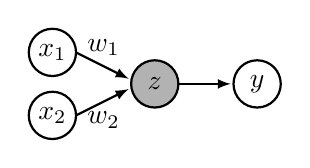
\begin{tikzpicture}[>=spaced latex]
\draw [thick, fill=white] (0,-0.4) circle [radius=0.3] node {$x_2$};
\draw [thick, fill=white] (0,0.4) circle [radius=0.3] node {$x_1$};
\draw [thick] [nn_edge] (0.3,-0.4) -- (1.0,-0.05) node[midway,below] {$w_2$};
\draw [thick] [nn_edge] (0.3,0.4) -- (1.0,0.05) node[midway,above] {$w_1$};
\draw [thick, fill=gray_neuron] (1.3,0) circle [radius=0.3] node {$z$};
\draw [thick] [nn_edge] (1.6,0) -- (2.3,0);
\draw [thick, fill=white] (2.6,0) circle [radius=0.3] node {$y$};
\end{tikzpicture}
%\end{minipage}
%}
%\end{figure}
}
}

\item When describing batches of tensors (as is commonly encountered in code), you may encounter $x_l[b,c,n,m]$ to represent an activation on layer $l$ of some network, with $b$ indexing batch element, $n$ and $m$ as spatial coordinates, and $c$ indexing channels.
\item Neuron values on layer $l$ of a deep net: $\mathbf{x}_{l}$
\item $x_{l}[n]$ refers to the $n$-th neuron on layer $l$. For neural networks with spatial feature maps (such as convolutional neural networks), each layer is an array of neurons, and we will use notation such as $x_{l}[n,m]$ to index the neuron at location $n,m$.
%\item For a network with spatial feature maps (e.g., a convolutional neural network), $x_{l}[c,i,j]$ refers to the $cij$-th neuron on layer $l$, where $i$ and $j$ index spatial position in a feature map, and $c$ indexes the channel.
\item The layer $l$ neural representation of the $i$-th datapoint in a dataset is written as $\mathbf{x}^{(i)}_{l}$.
\item We will also use $\xin$ and $\xout$ when we are describing a particular layer or module in a neural net and wish to speak of its inputs and outputs without having to keep track of layer indices.
\item For signals with multiple channels, including neural network feature maps, the first dimension of the tensor indexes over channel. For example, in $\mathbf{x} \in \mathbb{R}^{C \times N \times M \times \ldots}$, where $C$ is the number of channels of the signal.
\item For transformers, we deviate from the previous point slightly, in order to match standard notation: a set of tokens (which will be defined in the transformers chapter) is represented by a $[N \times d]$ matrix, where $d$ is the token dimensionality.
\end{itemize}


\subsection*{Probabilities}

We will sometimes not distinguish between random variables and realizations of those variables; which we mean should be clear from context. When it is important to make a distinction, we will use nonbold capital letters to refer to random variables and lowercase to refer to realizations.

Suppose $X, Y$ are discrete random variables and $\mathbf{x}, \mathbf{y}$ are realizations of those variables. $X$ and $Y$ may take on values in the sets $\mathcal{X}$ and $\mathcal{Y}$, respectively.
\begin{itemize}
    \item $a = p(X = \mathbf{x} \given \ldots)$ is the probability of the realization $X = \mathbf{x}$, possibly conditioned on some observations ($a$ is a scalar).
    \item $f = p(X \given \ldots)$ is the probability distribution over $X$, possibly conditioned on some observations ($f$ is a function: $f: \mathcal{X} \rightarrow \mathbb{R}$). If $\mathcal{X}$ is discrete, $f$ is the \emph{probability mass function}. If $\mathcal{X}$ is continuous, $f$ is the \emph{probability density function}.
    %\item $a = p(X = x | \overset{R}{y} = y)$ is the probability of the realization $\overset{R}{x}=x$ given $\overset{R}{y}=y$ ($a$ is a scalar).
    %\item $f = p(\overset{R}{x} | \overset{R}{y} = y)$ is the probability distribution over $\overset{R}{x}$ given $\overset{R}{y}=y$ ($f: \mathcal{X} \rightarrow \mathbb{R}$).
    %\item $f = p(\overset{R}{x} = x | \overset{R}{y})$ is a function with the property $f(y) = p(\overset{R}{x} = x | \overset{R}{y} = y)$ ($f: \mathcal{Y} \rightarrow \mathbb{R}$).
    %\item $p(\overset{R}{x} | \overset{R}{y})$ is the conditional probability distribution of $\overset{R}{x}$ given $\overset{R}{y}$ ($f: \mathcal{X} \times \mathcal{Y} \rightarrow \mathbb{R}$).
    %\item $p(x)$ is shorthand for $p(\overset{R}{x} = x)$.
    %\item $p(x|y)$ is shorthand for $p(\overset{R}{x} = x | \overset{R}{y} = y)$.
    %\item Suppose we have defined a named distribution, e.g., $p_{\theta}$; then referring to $p_{\theta}$ on its own is shorthand for $p(\overset{R}{x})$. This often comes up in expressions like $x \sim p_{\theta}$, which refers to $\overset{R}{x}$ as being distributed as $p_{\theta}(\overset{R}{x})$.
    %\item $p(\overset{R}{x} | y)$ is shorthand for $p(\overset{R}{x} | \overset{R}{y} = y)$
    \item $p(\mathbf{x} \given \ldots)$ is shorthand for $p(X = \mathbf{x} \given \ldots)$.
    %\item $p(\ldots | y)$ is shorthand for $p(\ldots | \overset{R}{y} = y)$.
    and so forth, following these patterns.
    \item Suppose we have defined a named distribution, for example, $p_{\theta}$, for some random variable $X$; then referring to $p_{\theta}$ on its own is shorthand for $p_{\theta}(X)$.
    \item We will write $Z \sim p$ to indicate a random variable whose distribution is $p$, and we will write $z \sim p$ to indicate a sampled realization of such a variable.
\end{itemize}
For continuous random variables, all the above notations hold except that they refer to probability densities and probability density functions rather than probabilities and probability distributions. We will sometimes also use the term ``probability distribution'' for continuous random variables, and in those cases it should be understood that we are referring to a probability density function.


\subsection*{Matrix Calculus Conventions}
\label{appendix:matrix_calc:notational_conventions}

In this book, we adopt the following conventions for matrix calculus. These conventions make the equations simpler, and that also means simpler implementations when it comes to actually writing these equations in code. Everything in this section is just definitions. There is no right or wrong to it. We could have used other conventions but we will see that these are useful ones.

Vectors are represented as column vectors with shape $[N \times 1]$:
\begin{align}
    \mathbf{x} = 
    \begin{bmatrix}
    x_1  \\
    x_2  \\
    \vdots \\
    x_N \\
    \end{bmatrix}
\end{align}
If $y$ is a scalar and $\mathbf{x}$ is an $N$-dimensional vector, then the gradient $\frac{\partial y}{\partial \mathbf{x}}$ is a row vector of shape  $[1 \times N]$:
\begin{align}
    \frac{\partial y}{\partial \mathbf{x}} =  
\begin{bmatrix}
    \frac{\partial y}{\partial x_1} & \frac{\partial y}{\partial x_2} & \cdots & \frac{\partial y}{\partial x_N} \label{backprop:scalar_vector_deriv}
\end{bmatrix}
\end{align}
If $\mathbf{y}$ is an $M$-dimensional vector and $\mathbf{x}$ is a $N$-dimensional vector then the gradient (also called the Jacobian in this case) is shaped as $[M \times N]$:
\begin{align}
\frac{\partial \mathbf{y}}{\partial \mathbf{x}} =  
\begin{bmatrix}
    \frac{\partial y_1}{\partial x_1} & \frac{\partial y_1}{\partial x_2} & \cdots & \frac{\partial y_1}{\partial x_N} \\
    \vdots & \vdots & \vdots & \vdots \\
    \frac{\partial y_M}{\partial x_1} & \frac{\partial y_M}{\partial x_2} & \cdots & \frac{\partial y_M}{\partial x_N}
\end{bmatrix}
\end{align}


Finally, if $\mathbf{W}$ is an $[N \times M]$ dimensional matrix, and $\mathcal{L}$ is a scalar, then the gradient $\frac{\partial \mathcal{L}}{\mathbf{W}}$ is represented as an $[M \times N]$ dimensional matrix (note that the dimensions are transposed from what you might have expected; this makes the math simpler later):
\begin{align}
    \frac{\partial \mathcal{L}}{\partial \mathbf{W}} &= 
        \begin{bmatrix}
            \frac{\partial \mathcal{L}}{\partial \mathbf{W}_{11}} & \ldots & \frac{\partial \mathcal{L}}{\partial \mathbf{W}_{N1}} \\
            \vdots & \ddots & \vdots \\
            \frac{\partial \mathcal{L}}{\partial \mathbf{W}_{1M}} & \ldots & \frac{\partial \mathcal{L}}{\partial \mathbf{W}_{NM}} \\
        \end{bmatrix} \label{backprop:scalar_matrix_deriv}
\end{align}
\marginnote{
We will often draw matrices and vectors to help visualize the operations. For example, if $N=3$ and $M=4$:\\[2pt]
\centerline{
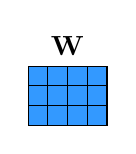
\begin{tikzpicture}
\draw[step=0.25cm,draw=black,fill=param_color_dark] (1.5,0) grid (2.5,-0.75) rectangle (1.5,0); \node at (2.0,0.25) {$\mathbf{W}$};
\end{tikzpicture}}
then, the gradient will have the form:\\[2pt]
\centerline{
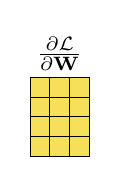
\begin{tikzpicture}
\draw[step=0.25cm,draw=black,fill=comp_graph_param_grad_bcolor] (0,0) grid (0.75,-1.0) rectangle (0,0); \node at (0.375,0.3) {$\frac{\partial \mathcal{L}}{\partial \mathbf{W}}$};
\end{tikzpicture}}
}[-.9in]

\subsection*{Conventions That Will Not Be Strictly Observed}
\begin{itemize}
\item We will often use $\mathbf{x}$ as the input to a function, and $\mathbf{y}$ as the output.
\item $f$, $g$, and $h$ are typically functions. The corresponding function spaces are $\mathcal{F}$, $\mathcal{G}$, $\mathcal{H}$.
\item Basis functions are $\phi$ and $\psi$.
\end{itemize}

\subsection*{Miscellaneous}
\begin{itemize}
\item The word ``dimension'' has two usages in the computational sciences. The first usage is as a coordinate in a multivariate data structure, for example, ``the $i$-th dimension of a vector'' or ``a 128-dimensional feature space.'' The second usage is as the shape of a multidimensional array, as in ``a 4D tensor.'' We will use both these meanings in this book and we hope the usage will be clear from context.
\end{itemize}


\mainmatter
\cleardoublepage



%%%%%%%%%%%%%%%%%%%%%%%%%%%%%%%%%%%%%%
%% CHAPTERS:
%\ifx\isEmbedded\undefined
%	% Loading common settings
%	\input{macros/common}
%	% Loading common variable definitions 
%	\input{macros/macros}
%	\begin{document} 
%\else
%\fi
%



\chapter{The Challenge of Vision}
\label{chap:challenge_of_vision}

%In order to write this book, we have adopted the following guideline: if you set up a goal and you fail at it, then just set up another goal. The best way of reaching the finish line is by bringing the finish line to where we are standing. And this is what we did. 

%Our initial goal was to write a large book that provided a good coverage of the field. Unfortunately, the field of computer vision is larger than Texas.  So, we decided to write a small book instead, limiting each chapter to no more than 5 pages. Such a goal forced us to really focus on the important concepts necessary to understand each topic. Unfortunately, we have failed at that too. The result of our failures is this book which, we hope, will motivate you to do better. 

%We believe that this short book is great for the following two reasons: 1) we do not have time to write a long book, and 2) you do not have time to read it. 

\section{Introduction}

%\marginnote{The word "Vision'' has its origin from the word {\em visionem}.}
Let's start with a simple observation: every day, when you wake up, you open your eyes and see. You see without any effort; you do not get tired after a few hours from seeing too much. The same happens with all the other senses. With them you perceive the world around you: you hear the birds or the car noises, you smell the breakfast and feel the touch of the sheets, and that keeps going on and on until the end of the day. But the most surprising fact is that your brain is continuously solving very complex tasks still unmatched by any artificial system.

The apparent simplicity of perceiving the world around us produces the false intuition that it will be easy to build a machine capable of seeing as humans do. Let's ignore the senses of hearing, touch, taste, and smell, and let's focus on the visual sense. Human vision is capable of extracting information about the world around us using only the light that reflects off surfaces in the direction of our eyes. The light that reaches our eyes does not tell us what object we are looking at. It only give us information about the amount of light reaching our eye from each direction in space. Our brains have to translate the information collected by millions of photoreceptors in our retinas into an interpretation of the world in front of us. What we see is different than the light that reaches our eyes, as visual illusions prove to us.
\marginnote{This book will focus on the visual sense. Nonetheless, the techniques introduced aren't exclusive to images and possess the versatility to be adapted for the processing of various other signal types.
}

Computer vision studies how to reproduce in a computer the ability to see. Since its origins, the study of vision has been an interdisciplinary study involving many disciplines (physics, psychology, biology, neuroscience, arts, and computer science).

The goal of a vision scientist is twofold: to understand how perception works and to build systems that can interpret the world around them using images (or image sequences) as input. In this chapter, we want to provide a broad perspective on {\bf vision science} and the multiple disciplines that contribute to it.


\section{Vision}

David Marr \cite{Marr82} defines vision as ``to know what is where by looking,'' and  adds ``vision is the process of discovering from images what is present in the world, and where it is.''

It is difficult to say exactly what makes understanding the mechanisms of vision hard as we do not have a full solution yet \cite{Cavanagh96}. In this section we will mention two  aspects that make vision hard: the structure of the input and the structure of the desired output.

What is the goal of vision? Our eyes are sensors, and for an agent that navigates and solves tasks in the world, the role of the sensor is to provide relevant information for solving the task. In the case of computer vision, we mostly study visual perception from a disembodied perspective. There is no agent and there is no task. This perspective makes the study of vision difficult.


\subsection{The Input: The Structure of Ambient Light}

From a light source, a dense array of light rays emerges in all directions. Before these light rays reach the eye, the light interacts with the objects in the world. Let's consider a single ray emerging from the light source (we will use here a simple geometric interpretation of the structure of light). If the light ray is not directed toward the eye, this ray will strike some surface in the world and, as result, a new set of rays will be emitted in many directions. This process will continue producing more and more interactions and filling the space. In the middle of the space the observer will sense only a subset of the light rays that will strike the eye. As a result of this complex pattern of interactions even a single ray will form a complex image in the eye of the observer.

%Figure~\ref{fig:lightRay} 
\Fig{\ref{fig:lightRay}} shows some pictures taken when illuminating a complex scene with a laser pointer that illuminate the scene with a narrow beam of light (this is the best approximation to the image produced by a single light ray that we could do at home).

\begin{figure}[t]
    \centerline{
        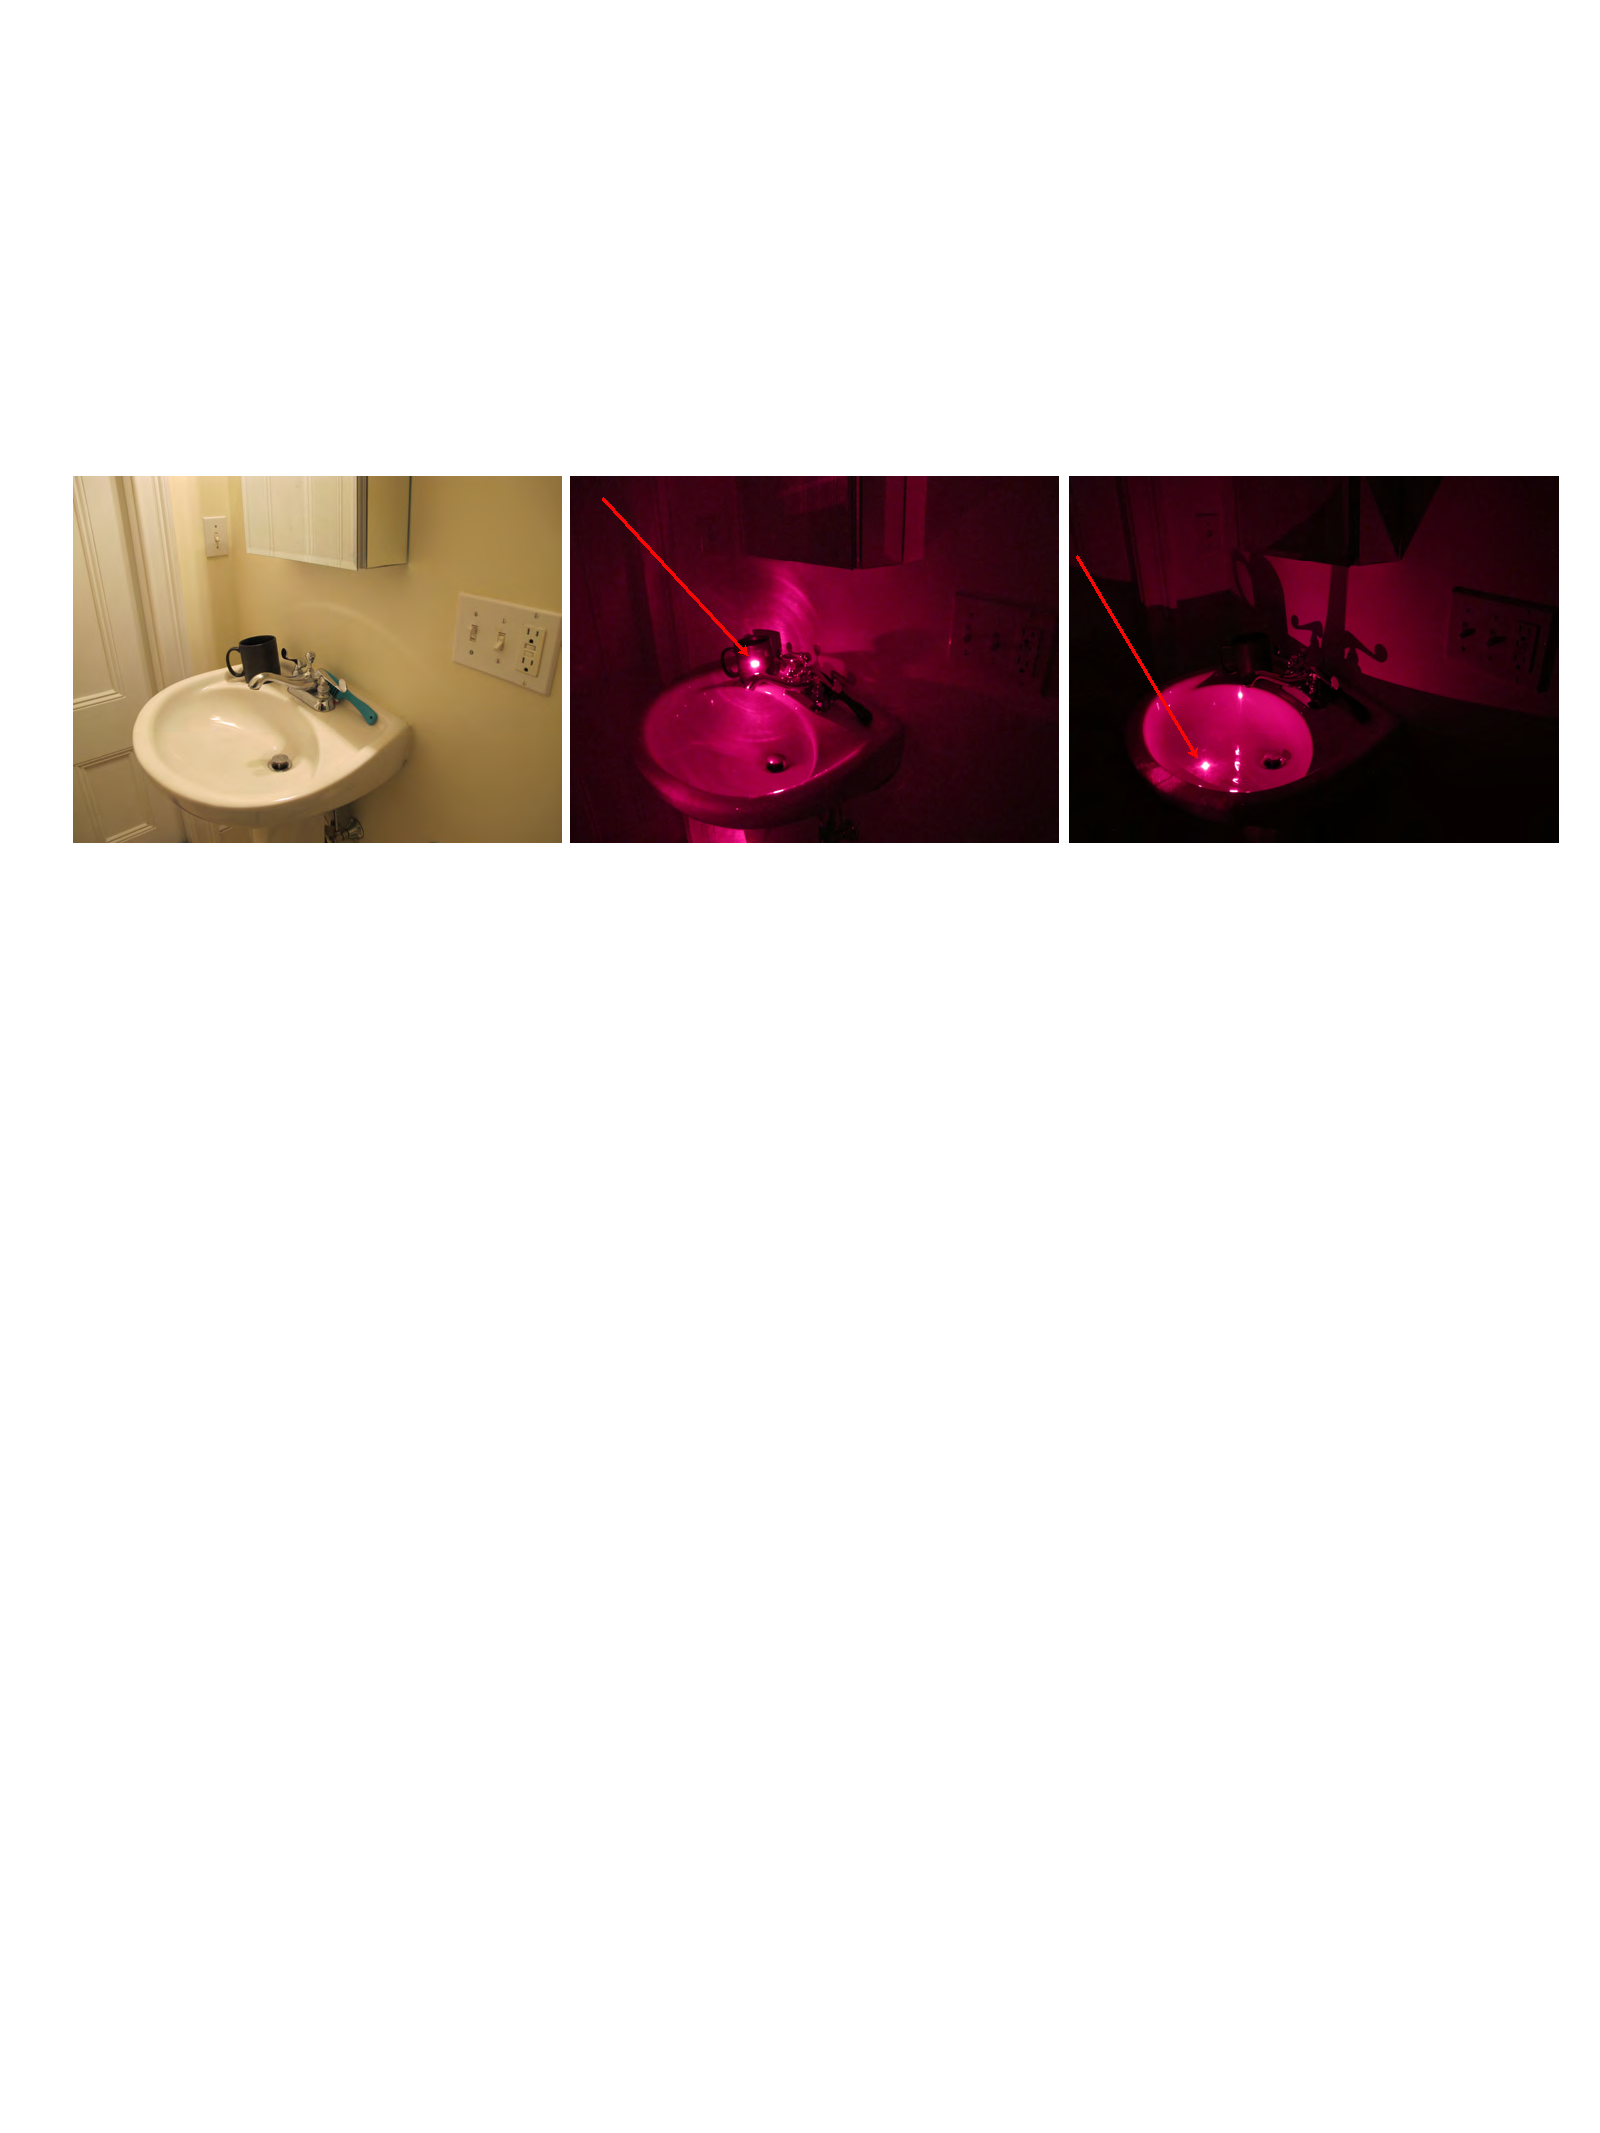
\includegraphics[width=1\linewidth]{figures/taxonomy/lightGray2.pdf}
    }
    \centerline{
        (a)\hspace{1.5in}(b)\hspace{1.5in}(c)
    }
    \caption{(a) Scene illuminated with a ceiling lamp. (b-c) Two images obtained by illuminating a scene with a laser pointer (the red line indicates the direction of the ray).}
    \label{fig:lightRay}
\end{figure}

The resulting images show the complexity of the interactions between the different surfaces. The sum of the contribution of all the light rays emitted by the light source will give rise to a natural looking picture. On each image, the approximate direction of the light beam produced by pointer is indicated by the red arrow in \fig{\ref{fig:lightRay}}{b-c}.

Despite the complexity of the structure of the ambient light (a term coined by James J. Gibson \cite{Gibson1966}) with multiple reflections, shadows, and specular surfaces (which provide incorrect disparity information to our two eyes), our visual system has no problem in interacting with this scene, even if it is among the first things that we see just after waking up.


The pattern of light filling the space can be described by the function:
\begin{equation}
    P (\theta, \Phi, \lambda, t, X, Y, Z)
\end{equation}
%\marginnote{We will study color in \chap{\ref{chapter:color}}.}
where $P$ is the light intensity of a ray passing by the world location $(X,Y,Z)$  in the direction given by the angle $(\theta, \Phi)$, and with wavelength $\lambda$ (we will study color in chapter [\ref{chapter:color}])
%chapter \ref{chapter:color}) 
at an instant in time $t$. This function, called the {\bf plenoptic function}
\index{Plenoptic function}
Edward H. Adelson
and James R. Bergen \cite{Adelson91}, contains all the information needed to describe the complete pattern of light rays that fills the space.
\marginnote{{\bf Plenoptic function}: Edward H. Adelson was going to call it
    the {\em holoscopic function}, but a well-known holographer told him that he would punch him in the nose if he called it that.}[.5in]
The plenoptic function does not include information about the observer. The observer does not have access to the entire plenoptic function, only to a small slice of it. In \chap{\ref{chapter:imaging}} we will describe how different mechanisms can produce images by sampling the ambient light in different ways.

For a given observer, most of the light rays are occluded. Without occlusion, vision would be a lot simpler. Occlusion is the best example of how hard vision can get. Many times, properly interpreting an image will require understanding what part is occluded (e.g., we know that a person is not floating just because the legs are occluded behind a table). Unfortunately, occlusions are common. In fact, there are more occluded surfaces than visible surfaces for any given observer.


Although recovering the entire plenoptic function would have many applications, fortunately, the goal of vision is not to recover this function.




\subsection{The Output: Measuring Light Versus Measuring Scene Properties}

Vision is not a deterministic process that analyzes the input images independently of our internal state. Even when two people look at the same thing they will have different {\bf visual awareness}. Our visual experience is greatly influenced by what we know, what we are doing, and what we expect to see.

If the goal vision were  simply to measure the light intensity coming from a particular direction of space (like a photometer) then things would be easy. However, the goal of vision is to provide an interpretation of the world in terms of ``meaningful'' surfaces, objects, materials, etc., in order to extract all the different elements that compose the scene (anything that will be relevant to the observer). This problem is hard because most of the information is lost and the visual system needs to make a number of assumptions about the structure of the visual world in order to be able to recover the desired information from a small sample of the plenoptic function. It is also hard because our understanding about what is relevant for the observer is incomplete.

The goal of vision is not to measure light intensities, but to extract scene properties relevant for the observer. \Fig{\ref{fig:measuringScene}} shows different images that illustrate that the human visual system is trying to recover the scenes that are the cause of those images.


\begin{figure}[t]
    \centerline{
        \includegraphics[width=1\linewidth]{figures/taxonomy/measuringScene2.eps}
    }
    \caption{We cannot shut down the automatic mechanisms that interpret these images not as light patterns but as pictures of real three-dimensional (3D) scenes. (a) Occluding figures, (b) R. Shepard's turning tables illusion, and (c) E. Adelson's Checkershadow illusion.
    }
    \label{fig:measuringScene}
\end{figure}

In \fig{\ref{fig:measuringScene}}{a}, we see a red square occluding a smaller blue square. But why do we see a blue square and not an L-shaped figure like the green shape on the top? If we assume that squares are typical in the world and that occlusions are common, then perceiving an occluded blue square is the most natural interpretation of the scene. Even though the green figure shows us that L-shaped figures are possible, we interpret the blue L-shaped figure as an occluded square. The next image, \fig{\ref{fig:measuringScene}}{b}, shows the ``turning tables illusion'' by Roger Shepard \cite{Shepard90}. In this illusion, both table tops have the same shape and size but one is rotated with respect to the other. The visual system insists in interpreting these objects as 3D objects giving the impression that the left table is longer than the table of the right.
And this perception can not be shut down even if we know exactly how this image has been generated. The third example, \fig{\ref{fig:measuringScene}}{c}, shows the ``checkershadow illusion'' by Adelson \cite{adelson1995checkershadow}. In this figure, the squares marked with A and B have the exact same intensity values. But the visual system is trying to measure the surface reflectance of the squares, removing the effect of the shadow to infer the true gray value of each square. As a result, the square in the shadow is perceived as being lighter than the square outside the shadow region, even though both have the same gray levels.

\marginnote{When looking at a two-dimensional (2D) picture, we automatically interpret it as a 3D scene if the right cues are present.}[-.0in]

%\subsection{Visual tasks}

The goal of vision is to provide the observer with information relevant to understanding the outside world and to enable them to solve other tasks such as navigating the world, interacting with other agents, and finding food. Tasks within computer vision include the following: detecting changes in the environment; motion estimation; object recognition and localization; recognizing materials; reading text and visual symbols; building 3D models from images; finding free space to move; finding other people; deciding if food is in good state; and understanding the behavior of animals. Not all of those tasks are at the same level. Some seem to require a lot of external knowledge while others seem solvable from the images alone.

\section{Theories of Vision}

%An evolution from cognition to computational approaches.

In this section we want to describe, with a few strokes, some of the theories of vision that have contributed to and shaped modern approaches. Think of this section as a travel brochure that will show you a few snapshots of a trip, but that's not intended to be a replacement for traveling yourself. You should read the books and papers that we will mention in this section, as they are the foundations on which this fascinating field has been built.

%% Books are full of insights and any summary, like the ones you will find here, fail at teaching what is really important. Our intention is to provide here enough motivation for you to conclude that it is worth going to the original books for inspiration. 


\subsection{The Origins of the Science of Perception}
%
% Source: https://www.researchcatalogue.net/view/1025487/1025488
% https://philosophy.ucla.edu/wp-content/uploads/2018/08/Burge-2011-Origins-of-Perception.pdf

How do we know what is in the world by looking at it? Understanding how an image of the world is getting into our minds has a long history that required contributions from many scientific disciplines (art, philosophy, physics, optics, biology, psychology, neuroscience, etc.).


Ancient humans probably knew that their image of the world originated in the eyes. It just takes closing your eyes or putting one hand in front of one eye to see the corresponding image disappear. In fact, chimpanzees and orangutans might also know that the eyes are the source of visual stimuli as they seem to do {\bf eye-gaze following} to understand what their companions  are paying attention to.
% Tomasello M, Call J, Hare B (1998) Anim Behav 55:1063–1069, pmid:9632490.
Humans learned to create astonishing images in caves with a degree of realism that indicates an understanding of colors, forms, shadows, and motion. They did not think that in order to create an image of a bison on the wall of the cave the only option was to attach a dead bison to the wall. They knew that a dynamic scene could be represented by static painting.  Paintings are a potent visual illusion that show that the image of the object does not need the object itself.

\marginnote{If you have never read the works of the Greek philosophers, please do. You will be astounded by how much they new about math and physics even though they lacked devices to confirm many of their hypothesis.}
How is information about the world being picked up by our eyes?
% http://www.yorku.ca/rsheese2/1010/perception.htm
% https://ircps.org/wp-content/uploads/2021/04/2004-01-02_Cooper.pdf
The Greeks had two competing theories: intromission theories and extramission (or emission) theories.


Early {\bf intromission} \index{Intromission theory}
theories (425 BC) believed that objects emitted copies of themselves (eidola or simulacra) that entered the eyes. This theory was defended by philosophers such as Demokritos, Epicurus, and Lucretius. However, it was unclear how objects could be sending copies when there were multiple observers, and how the copies did not interfere with each other. It was also unclear how copies of large objects could fit into the eye.

    {\bf Extramission} theory\index{Extramission theory}, started with Empedocles \cite{kalderon2015form} and was later followed by Plato and Euclid among others. Empedocles (approx. 494--434 BC) provided one the first theories of vision in his poem ``On Nature'', and introduced many other influential ideas such that all things are composed or four elements: fire, earth, air, and water. He said that the eye contained the four elements and that the fire was responsible of creating {\bf rays} that emanated from the eyes, like fingers that sensed the world. The extramission theory explained why sometimes eyes shined at night, in particular cat's eyes, which were assumed to contain so much fire that even humans could see it occasionally. Of course, now we know that the when cats' eyes appear to shine, they
are reflecting light from other sources, but without a theory of light and reflection it made sense to believe that one was observing rays emitted by the eyes.
\marginnote{The extramission theory attributed the glow observed in cat eyes to the presence of fire inside them.
    \\[6pt]
    \centerline{
        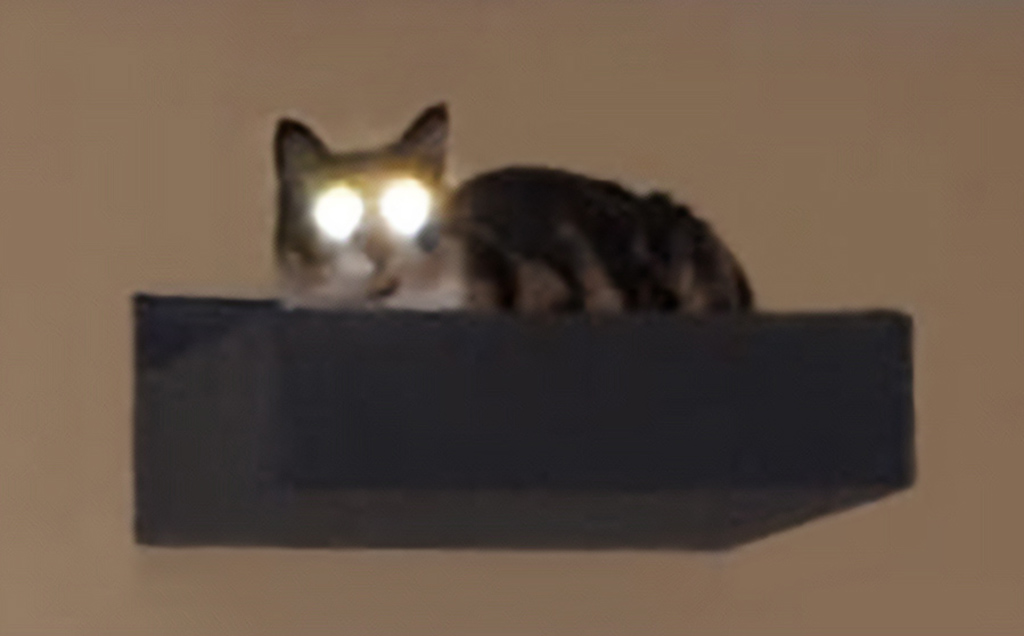
\includegraphics[width=4cm]{figures/taxonomy/cat_eyes.jpg}
    }
}

%\marginnote{Plato's dialogues are fictitious conversations among philosophers arguing about several topics.}
Plato’s theory of vision (427--347 BC) was very influential. Plato's theory contained both intromission and extramission elements. The following is a fragment of Plato's dialog \booktitle{Timaeus} \cite{Plato360bc}, which provides a description of how the flow produced by the internal fire in the eyes interacts with the external fire to produce sight:

%%``{\em 

\begin{quote}
    And of the organs they first contrived the eyes to give light, and the principle according to which
    they were inserted was as follows: So much of fire as would not burn,
    but gave a gentle light, they formed into a substance akin to the
    light of every-day life; and the pure fire which is within us and
    related thereto they made to flow through the eyes in a stream smooth
    and dense, compressing the whole eye, and especially the centre part,
    so that it kept out everything of a coarser nature, and allowed to
    pass only this pure element. When the light of day surrounds the stream
    of vision, then like falls upon like, and they coalesce, and one body
    is formed by natural affinity in the line of vision, wherever the
    light that falls from within meets with an external object. And the
    whole stream of vision, being similarly affected in virtue of similarity,
    diffuses the motions of what it touches or what touches it over the
    whole body, until they reach the soul, causing that perception which
    we call sight. But when night comes on and the external and kindred
    fire departs, then the stream of vision is cut off; for going forth
    to an unlike element it is changed and extinguished, being no longer
    of one nature with the surrounding atmosphere which is now deprived
    of fire: and so the eye no longer sees, and we feel disposed to sleep.
\end{quote}

%%}''
% excerpt from http://classics.mit.edu/Plato/timaeus.1b.txt

Plato considered the sense of vision as being worse than touch because vision could only sense the part that was facing the observer. Therefore, according to Plato, one could not trust the sense of vision. However, Aristotle (384--322 BC), Plato's student, was critical of the extramission theory and pointed out that the stars were too far away for rays from the eyes to reach them (an argument also used by Euclid). Aristotle went further and suggested that only some objects are light sources (e.g., fire) and the other objects reflect the rays that hit the eyes \cite{Aristotle350bc}. He also criticized the belief that the eye had fire inside. Instead, Aristotle defended the idea that the element of perception had to be water as vision needed a transparent element.


Euclid (325 BC), a Greek mathematician, provided the first mathematical theory of vision, giving a mathematical description of how the emitted rays by the eye traveled on {\bf straight lines} and formed a cone that reached the scene.
\marginnote{Modeling light as traveling along straight lines was a major discovery. This simple model of light sets the foundation upon which image formation, scene geometry, and computer vision rests.
    %\begin{figure}
    %\centerline
    \\[6pt]
    \centerline{
        %\includegraphics[width=1\linewidth]{figures/taxonomy/eye_w_fire_aina.eps}
        \includegraphics[width=4cm]{figures/taxonomy/eye_w_fire_aina.eps}
        %}
        %\end{figure}
    }
}
He listed the following seven axioms of light, extracted from \cite{Burton1945}:
% from http://philomatica.org/wp-content/uploads/2013/01/Optics-of-Euclid.pdf
\begin{quote}
    \begin{enumerate}
        \item Let it be assumed that lines draw directly from the eye pass through a space of great extent;
        \item and that the form of the space included within our vision is a cone, with its apex in the eye and its base at the limits of our vision;
        \item and that those things upon which vision falls are seen, and that those things upon which vision does not fall are not seen;
        \item and that those things seen within a larger angle appear larger, and that those seen within a smaller angle appear smaller, and those seen within equal angles appear to be of the same size;
        \item and that things seen within the higher visual range appear higher, while those within the lower range appear lower;
        \item and, similarly, that those seen within the visual range on the right appear on the right, while those within that on the left appear on the left;
        \item but that things seen within several angles appear to be more clear.
    \end{enumerate}
\end{quote}

Starting from those axioms, in his paper ``Optics'' \cite{Burton1945}, Euclid describes many different ways to use geometric reasoning to measure the size of objects in the world using the properties of light and vision.
One example of the application of his theory is shown in \fig{\ref{fig:euclid}}.
The description of the figure in the original text reads as follows:
%\begin{quote}
``To know how great is a given elevation (AB) when the sun is shining. Let the eye be D, and let GA be a ray of the sun falling upon the end of line AB, and let it be prolonged as far as the eye D. And let DB be the shadow of AB. And let there be a second line, EZ, meeting the ray, but not at all illuminated by it below the end of line at Z. So, into the triangle ABD has been fitted a second triangle, EZD. Thus, as DE is to ZE, so is DB to AB. But the ratio of ED to ZE is known. Moreover, DB is known; so, AB is also known''
%\end{quote} 
\cite{Burton1945}.


\begin{figure}[t]
    \centerline{
        \includegraphics[width=0.6\linewidth]{figures/taxonomy/euclid.eps}
    }
    \caption{Adapted from Euclid (325 BC). The color and text, added here for clarity, is not part of the original figure \cite{Burton1945}.
        %The description of the figure reads \cite{Burton1945}: ``{\bf To know how great is a given elevation (AB) when the sun is shining}. Let the eye be D, and let GA be a ray of the sun falling upon the end of line AB, and let it be prolonged as far as the eye D. And let DB be the shadow of AB. And let there be a second line, EZ, meeting the ray, but not at all illuminated by it below the end of line at Z. So, into the triangle ABD has been fitted a second triangle, EZD. Thus, as DE is to ZE, so is DB to AB. But the ratio of ED to ZE is known. Moreover, DB is known; so, AB is also known."
    }
    \label{fig:euclid}
\end{figure}


\marginnote{Euclid's work set the basis of {\bf perspective}, and his discoveries influenced thinkers and artists in the following centuries.}[-0.05in]


Many other Greek philosophers and mathematicians
contributed to a deeper understanding of light. Hero of Alexandria (10-70), in the work \textbf{Catoptrica}, postulated that light propagated in straight lines and also described an early version of the {\bf law of reflection}: light will follow the shortest path between two points, which means that the angle of incidence is the same as the angle of departure. Ptolemy described how light changed direction (i.e., {\bf refraction}) when changing medium (e.g., from air to water). Few other discoveries about vision between the first and tenth centuries survive.
\marginnote{Credit assignment is unclear. For instance, early versions of the law of reflection are credited to Heron, Ptolemy, Archimedes, Plato, and was potentially known to others before \cite{10.2307/225870}.
    % https://www.jstor.org/stable/225870
}



In the late tenth century Hasan Ibn al-Haytham's work transformed the initial Greek theories into a true scientific discipline, inspiring many of the works that followed, even through Johannes Kepler.  Ibn al-Haytham (965--1040 AD), known as Alhacen in the Latin world, published the \booktitle{Book of Optics} \cite{2001alhacen} between the years 1028 and 1038. This book is considered by many the beginning of the scientific method. In his Book of Optics, Ibn al-Haytham describes how light rays bounce of objects in all directions and that the rays only become visible when they reach the eye perpendicularly. He described the pinhole camera and invented the {\bf camera obscura}.
\index{Camera obscura}


\begin{figure}[t]
    \centerline{
        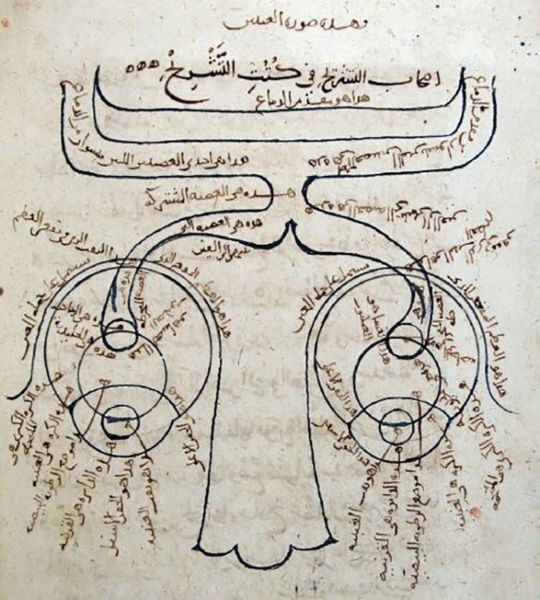
\includegraphics[width=0.5\linewidth]{figures/taxonomy/Alhazen1652.png}
        % https://www.discovermagazine.com/mind/visions-of-the-brain-ancient-and-modern
        % http://glps2.org/wiki/index.php?title=File:Alhazendiagramnerves.gif
        % https://www.aspetar.com/journal/viewarticle.aspx?id=293#.Yo42TGDMJO5
    }
    \caption{Alhacen's diagram of the eyes and the optic nerve (\booktitle{Book of Optics}), drawn around the year 1027. It is one of the first drawings of the visual system. {\em Source}: MS Fatih 3212, vol. 1, fol. 81b, Süleimaniye Mosque Library, Istanbul.}
    \label{fig:Alhacen}
\end{figure}


Ibn al-Haytham rejected the extramission theory. He argued that sight could be explained by the light rays emitted by objects and that it was not necessary to assume that the eye emitted rays. Ibn al-Haytham's work built upon the work of Ptolemy, Euclid, Galen, and Aristotle, although little is known about the exact sources of inspiration as manuscripts at that time did not include citations to previous work and it was rare when other scientists were cited by name. Ptolemy believed that distance between the eye and an object could be measured by feeling the length of a ray of light (thus requiring a single eye), while Ibn al-Haytham showed experimentally that both eyes were needed to perceive depth \cite{2001alhacen}.



Kepler (1604 AD), building on Alhacen's work, provided the first complete description of how images are formed in the retina in \booktitle{Astronomiae Pars Optica}
%Ad Vitellionem paralipomena 
\cite{Martens2001-MAROPT-2}. Kepler understood {\bf lenses} and how the eye projected a reverse picture into the retina. Kepler understood the role of the crystalline lens as the focusing element of images in the eye, in contrast with previous theories that believed that the crystalline lens was the sensitive element selecting only the perpendicular rays that reached the eye.



\subsection{Helmholtz: Perception as Inference}


Hermann von Helmholtz (1821--1894) was a German scientist and philosopher. While he wanted to study physics, he trained as a physician at the urging of his father \cite{Shapin2019}, then went on to make important contributions in philosophy, physics, audition, color theory, and visual perception.


With Thomas Young, he codeveloped the theory of {\bf trichromacy},
\index{Trichromacy}
that the eye has three classes of receptors, each sensitive to different wavelengths of light.  \marginnote{
    \centerline{
        
\includegraphics[width=3cm]{figures/taxonomy/trichromacy_helmholtz.eps}
    }
}

He measured the speed of transmission of nerves (24.6--38.4 m/s \cite{wikiHelmholtz2021}, previously thought to be unmeasurably fast \cite{Shapin2019}).  He also developed the ophthalmascope, shown in \fig{\ref{fig:helmholtz}}, an instrument to observe the retina of the human eye. The key of the ophthalmascope was to see the need for colinear viewing and illumination directions. \Fig{\ref{fig:helmholtz}}{a} shows a schematic illustration of Helmholtz's opthalmoscope, viewed from above.  The glass plates along the diagonal, labeled $a$ in the figure, allow for viewing the eye under study by the opthalmologist while reflecting illumination from a light source into the eye. \Fig{\ref{fig:helmholtz}}{b} shows a drawing by Helmholtz of an image from the ophthalmoscope, showing blood vessels (in background) and branches of the retinal artery and vein over the optic nerve (center).


\begin{figure}[t]
    \centerline{
        \sublabel{a}{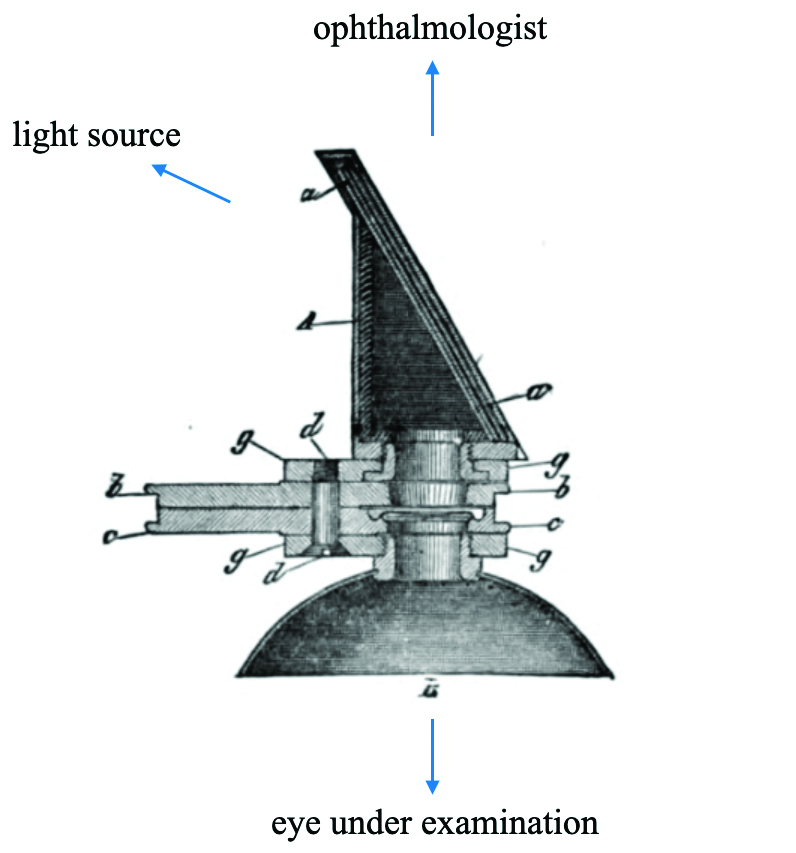
\includegraphics[width=0.45\linewidth]{figures/taxonomy/helmholtzOpth1Labeled.jpg}}
        \sublabel{b}{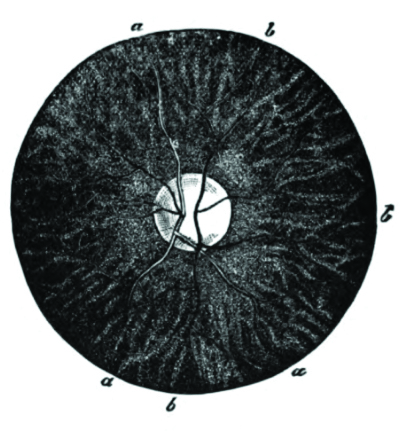
\includegraphics[width=0.44\linewidth]{figures/taxonomy/helmholtzOpth3.jpg}}
    }
    \caption{Hermann von Helmholtz invented the ophthalmoscope at age 29.
        %The key was to see the need for colinear viewing and illumination directions. (a) Schematic illustration of Helmholtz's opthalmoscope, viewed from above.  The glass plates along the diagonal, labeled $a$ in the figure, allow for viewing the eye under study by the opthalmologist while reflecting illumination from a light source into the eye. (b) Drawing by Helmholtz of an image from the ophthalmoscope, showing blood vessels (in background) and branches of the retinal artery and vein over the optic nerve (center).  
        Images from \cite{Helmholtz1925}.}
    \label{fig:helmholtz}
\end{figure}


Helmholtz was also an important theorist in visual perception.  He wrote \cite{Helmholtz62},
%``
\begin{quote}
    The general rule determining the ideas of vision that are formed whenever an impression is made on the eye, is that {\em such objects are always imagined as being present in the field of vision as would have to be there in order to produce the same impression on the nervous mechanism, the eyes being used under ordinary normal conditions}.
    %''
\end{quote}
%(Emphasis in the original) \cite{Helmholtz62}.

Thus, the mind makes perceptions out of sensations \cite{Shapin2019}, finding representations of the object most likely to explain the sensory input \cite{Wandell95}.  This viewpoint relates to {\bf Bayesian methods} for computer vision inference.

In his introduction, ``Concerning the Perceptions in General,'' he continued \cite{Helmholtz62}:
\begin{quote}
    %``
    Still, it may be permissible to speak of the psychic acts of ordinary perception as {\em unconscious conclusions}, thereby making a distinction of some sort between them and the common so-called conscious conclusions.
\end{quote}
%''
He added that when an astronomer computes the position of stars in space, based on observations, this is a conscious conclusion. When you press on the eye and see light, that is an unconscious conclusion about what is in the world, given the responses of your eye. This unconscious inference is the topic of computer vision.


Helmholtz emphasized the active role of the viewer in perception \cite{Helmholtz62},
\begin{quote}
    If the objects had simply been passed in review before our eyes by some foreign force without our being able to do anything about them, probably we should never have found our way about amid such an optical phantasmagoria ... But when we notice that we can get various images of a table in front of us simply by changing our position; and that we can sometimes have one view and sometimes another, just as we like at any time ... Thus by our movements we find out that it is the stationary form of the table in space which is the cause of the changing image in our eyes.
\end{quote}
This foreshadows some unsupervised learning methods common in computer vision today.


\subsection{Gestalt Psychology and Perceptual Organization}
% https://www.ncbi.nlm.nih.gov/pmc/articles/PMC3482144/
% https://www.sciencedirect.com/science/article/pii/S0042698900000869?via%3Dihub


Gestalt psychology
\index{Gestalt psychology}
started around 1912, with the publication of “Experimental Studies of the Perception of Movement” by Max Wertheimer \cite{wertheimer1912experimentelle}. In this paper Wertheimer introduced the {\bf phi phenomenon}, a visual illusion that consists in presenting two images with a vertical bar at different locations in rapid succession giving the impression that there is continuous motion between them \cite{steinman2000phi}.
\marginnote{
    \centerline{Frame 1 ~~~~~~~~~~~~~~~~~~~~~~~~~~~~~~~~~~~~~~~~~~~~~Frame 2}
    ~\\[-4pt]
    \centerline{
        \includegraphics[width=.35\linewidth]{figures/taxonomy/phi_phenomenon_1.eps}
        ~~
        \includegraphics[width=.35\linewidth]{figures/taxonomy/phi_phenomenon_2.eps}
    }
}
Wertheimer, together with Kurt Koffka and Wolfgang Köhler, postulated that perceived motion was a new phenomenon that is not present in the individual stimuli (the two flashing frames) and that what we perceive is the whole event as a single unit (continuous motion). Gestalt psychology extended this interpretation to explain many other visual phenomena and emerged as a reaction of the existing trend that said that for psychology to be a science it had to decompose stimuli into its constituent elements. Gestalt theory argued that perception is about wholes more than it is about parts.



Wertheimer introduced the problem of {\bf perceptual organization}.
\index{Perceptual organization}
Perceptual organization studies how our visual system organizes individual visual features (i.e., colors, lines, ...) into coherent objects and wholes. Wertheimer proposed a set of rules
used by the visual system to organize elements on a simple display. He showed sets of dots and lines disposed in different arrangements, as shown in \fig{\ref{fig:gestalt}}, to find out when those elements were grouped together into larger elements.


\begin{figure}[t]
    \centerline{
        \includegraphics[width=1\linewidth]{figures/taxonomy/gestalt.eps}
    }
    \caption{Gestalt grouping rules for perceptual organization. Most of the examples are recreated from \cite{Palmer1999}. The closure pattern is from Koffka \cite{Koffka1935}, who modified it from Kohler.}
    \label{fig:gestalt}
\end{figure}

Gestalt psychologists called {\bf grouping laws}
\index{Gestalt psychology!Grouping laws}
the visual cues they uncovered. However, they are not strictly laws and not all grouping cues are equally strong. Some of the most important laws are as follows:
\begin{itemize}
    \item Law of {\bf proximity}: Items that are nearby are more likely to group together. From \fig{\ref{fig:gestalt}}, we can see that groupings a-b, c-d, e-f, and g-h are stronger than b-c, d-e, and f-g. With some effort one can group the items according to the second arrangement, but it is hard to sustain that grouping perceptually. The law of proximity is affected by the similarity of the items.
    \item Law of {\bf similarity}: Elements that have similar features (color, size, orientation) also group together, even when they are all equally distant.
    \item Law of {\bf closure}: We are very familiar with the fact that when a line forms a closed figure, we do not simply see a line, we see a shape. The example shown in \fig{\ref{fig:gestalt}} shows how closure wins over proximity. The vertical lines are closer for the grouping a-b. However, we group them as b-c, d-e, and f-g.
    \item Law of {\bf good continuation}: Edges are likely to be smooth. Lines that follow each other pointing in the same direction are likely to be grouped together. For instance, an X-shape is perceived as two lines that cross each other instead of perceiving it as a V-shape on top of an inverted V.
          \marginnote{Law of good continuation. The following shape:
              \\[6pt]
              \centerline{
\includegraphics[width=.15\linewidth]{figures/taxonomy/grounding_gc_1.eps}}
              has two possible groupings:
              \\[6pt]
              \centerline{
\includegraphics[width=.35\linewidth]{figures/taxonomy/grounding_gc_2.eps}}
              The law of good continuation says that the one on the left is
              the one an observer perceives (although we just see an X and not two lines crossing each other...)
          }[-.2in]

    \item Laws of {\bf parallelism}, and {\bf symmetry}: There are many other grouping cues with different strengths that induce clustering between visual elements.
    \item {\bf Common fate}: Motion is a very important grouping cue. When two elements have a common motion (accelerations, direction, rate of change) they tend to group together.
          %\item Law of prägnanz or simplicity
    \item {\bf Past experience}: Items grouped in the past are more likely to be perceived as a group in the future.
          %Palmer \cite{Palmer1999} highlighted the importance of this grouping introduced by Wertheimer.
\end{itemize}

In complex displays, one will expect that multiple of these grouping cues will be present. Gestalt theory not did quantitatively address how grouping cues will balance each other when they were in conflict. Stephen Palmer \cite{Palmer94} measured the strength of these grouping cues and introduced new ones.

Gestalists also studied the problem of {\bf lightness perception}.
\index{Lightness perception}
\marginnote{
    {\bf Lightness} is a perceptual quantity that is influenced by both the perceived reflectance and the perceived illumination of a surface \cite{Adelson99}.
    %Ted Adelson \cite{Adelson99} defines {lightness} as "the perceived reflectance of a surface. It represents the visual system’s attempt to extract reflectance based on the luminances in the scene". And Reflectance "is the proportion of incident light that is reflected from a surface."
}
For a wonderful book on lightness perception, we refer the reader to \cite{gilchrist2006}, and the work of Edward Adelson \cite{Adelson99}. Adelson defines lightness as ``the visual system’s attempt to extract reflectance based on the luminances in the scene.''

Gestalt psychologists said that the perception of lightness on an image patch is a function of the context. One has to take into account the grouping laws (perceptual organization) in order to explain the perceived lightness on a display. Koffka \cite{Koffka1935} introduced the {\bf Koffka ring}, a beautiful illusion to illustrate the power of perceptual grouping to explain lightness perception (\fig{\ref{fig:koffka_ring}}).
\marginnote{Kurt Koffka, born in Berlin in 1886, published his \booktitle{Principles of Gestalt Psychology} in 1935, after moving to the USA in 1924.}

\begin{figure}[t]
    \centerline{
        \includegraphics[width=1\linewidth]{figures/taxonomy/koffka_ring.eps}
    }
    \caption{(a) A ring of uniform gray. (b) Koffka ring and (c) a variant introduced by Adelson \cite{Adelson99}.  In all the examples, the two sides of the ring are identical.}
    \label{fig:koffka_ring}
\end{figure}

In each display, the two sides of the ring have the same gray level. Depending on the spatial configuration of the two sides, their lightnesses appear very different. In \fig{\ref{fig:koffka_ring}}{a} the ring appears as solid gray. In \fig{\ref{fig:koffka_ring}}{b} splitting the figure into two halves by an interleaving white space makes the two sides of the ring look different. \Fig{\ref{fig:koffka_ring}}{c} shows a variant of the Koffka ring proposed by Adelson \cite{Adelson99} where the grouping cues create a stronger effect. One can conclude from this experiment that lightness perception is not a local process and that it involves considering the context and the principles of grouping.



%Koffka, born in Berlin in 1886, moved to USA in 1924. In 1935, Koffka published his Principles of Gestalt Psychology.


Another striking proof of the importance of perceptual organization is the visual phenomenon of {\bf amodal completion}.
\index{Perceptual organization!Amodal completion}
As discussed in the introduction, in \fig{\ref{fig:measuringScene}}{a} we see a red square on top of a blue square. Even though the blue square is occluded by the red square, we see it as a square. The green geometric figure is identical to the blue one but the gap breaks the illusion of occlusion and we do not perceive it as a square anymore. This phenomenon of perceiving a whole object when only a part is visible is called {\bf amodal completion}. The word {\em amodal} means that we have perception without using any direct perceptual modality.

Amodal completion is something we do all the time when we explore a scene. Most of the objects that we see are partially occluded and we use amodal completion to extend the object behind the occlusion.

    {\bf Modal completion}
\index{Perceptual organization!Modal completion}
is a related visual phenomenon that happens when we see an induced object appear in front of others. \Fig{\ref{fig:kanizsa}} shows several examples of modal and amodal completion. A beautiful visual illusion that illustrates modal completion is the {\bf Kanizsa triangle}, shown in \fig{\ref{fig:kanizsa}}{d}. In this case, we see a triangle that is not really there.


\begin{figure}
    \centerline{
        \includegraphics[width=1\linewidth]{figures/taxonomy/kanizsa.eps}
    }
    \caption{Amodal and modal completion. (a) is this 13 or an occluded B? (b) By adding boundaries to the occluder, the letter B becomes clearer. (c) How many squares are there? Behind the occluder are there two squares or just one rectangle? (d) Kanizsa triangle. Illusory contours appear at the triangle sides.}
    \label{fig:kanizsa}
\end{figure}

The Kanizsa triangle shows both amodal and modal completion. The circles are seen by amodal completion and the triangle appears as modal completion. Modal completion produces {\bf illusory contours} to appear in the image. Some observers report that the triangle on top is brighter than the surrounding background and that illusory contours appear at the triangle sides.
\index{Perceptual organization!Illusory contours}

\marginnote{Gaetano Kanizsa \cite{kanizsa79} studied how perceptual organization could be used to see what is not there.}

% Specially remarkable is the Kanizsa triangle, Figure.~\ref{fig:kanizsa}.d. The circles are amodally completed, the invisible triangle is modally completed. 


%Organization in Vision: Essays on Gestalt Perception, Praeger Publishers, 1979

Perceptual organization remains an intriguing and rich area of research with many visual mechanisms still poorly understood. The list of principles of perceptual organization discovered by the gestalt theory have impacted a lot of modern research in computer vision, in particular in the domain of {\bf image segmentation} \cite{Malik90}.


\subsection{Gibson's Ecological Approach to Visual Perception}

While previous theories of perception considered that the simplest scenario to study vision was assuming a static camera taking a snapshot in a controlled lab setting, James J. Gibson postulated that, to understand vision, one should take an {\bf ecological approach to visual perception} \cite{Gibson1979}. The study of the eye should be done in the context of the body that supports it and the world it lives in.

Experimental science based in simple visual stimuli allowed for measuring quantities, reporting results, and reproducing findings, but the simple stimuli were very limiting. Dealing with real-world stimuli is messy, and no one had good theories on how to use them experimentally. Gibson argued that, to understand perception, the experimental lab should be like real life. Many of the displays used by gestalt psychologists were too simple and unlikely to occur in the real world. They provide useful knowledge, but fall short of unraveling the true nature of the visual system.

The environment should be studied by means of ecological properties, and not by using physical laws. That is, by understanding what quantities and processes of the environment are relevant for the observer. An ecological description of the environment describes it in terms of medium (air or water), substances (rocks, metal, wood, etc.), and surfaces (which separate medium from substances), together with the notions of change and persistence.
Gibson considers those concepts more relevant to the study of perception than the notions of space, matter, and time, which have their origin in classical physics but have little relevance for the observer. The dominant role of the observer in Gibson's theory is illustrated in how the environment is understood: water is substance for terrestrial animals, and it is the medium for aquatic animals.
The {\bf ground plane}
is the most important surface for terrestrial animals, it is the center of their perception and behavior. The ground provides the support for action and a reference for perception. Other notions of ecological importance are the concepts of {\em layout}, {\em place}, and {\em enclosure}.
\marginnote{Drawing by Gibson showing how few lines induce a strong 3D percept of a ground plane.
    \\[6pt]
    \centerline{
        \includegraphics[width=.3\linewidth]{figures/taxonomy/gibson_cover_the_perception_of_visual_world.eps}
    }
}


Gibson also made a distinction between the light studied by optical physics and the one that is relevant for perception, which he called {\bf ecological optics}.
\index{Ecological optics}
According to Gibson, physicists are interested in studying light in simplified settings such as the light emitted by point sources that send rays into an infinite space, or that interact with surfaces or lenses once. Ecological optics instead studies the light that converges into the observer, which is the result of countless interactions with all the surfaces in a messy environment. The {\bf ambient optic array} is the set of light rays that converge into a point of observation. And this point of observation can be occupied by an observer who will move around the world. This moving ambient optic array will contain information about the environment and also about the observer themself (\fig{\ref{fig:gibson_bird}}).


\begin{figure}[t]
    \centerline{
        \includegraphics[width=0.7\linewidth]{figures/taxonomy/gibson_bird.eps}
    }
    \caption{The flow pattern in the optic array of a bird flying over the earth provides information about the environment and also about the bird. Figure recreated from \cite{Gibson1966}.}
    \label{fig:gibson_bird}
\end{figure}

Another key concept in Gibson's theory is the notion of {\bf affordance} \index{Affordance}
introduced by Gibson in 1966 \cite{Gibson1966}. A {\em path} affords locomotion from one point to another, an {\em obstacle} affords collision, and a {\em stairway} affords both descent and ascent.
%The Senses Considered as Perceptual Systems, 1966
An {\em object} is a substance enclosed by a surface. The affordance of an object is generally a direct consequence of its properties: a hollow object can contain substances, a detached object affords carrying, an object with a sharp edge affords cutting, and so on. Animate objects are controlled by internal forces, and they afford social interaction.


Gibson's theory of visual perception postulates that the ambient optic array is very rich and contains all the information needed to perceive the environment.  {\bf Direct perception} is the process of {\bf information pickup} directly from the ambient array. This is in contrast with other theories of visual perception that assume that the input stimuli
\marginnote{Gibson did not like the term {\bf stimuli} because it implied that the environment stimulates the observer. For Gibson, it is important to stress that the observer is only picking up information.}[-.3in]
is very impoverished and that perception is {\bf indirect} as it has to be complemented by additional processes.
The indirect theory of perception is the most common one. However, the important message to learn here is that, when building a perceptual system, the richer the input is, one might hope that the solution to the perception problem will be simpler.
% For a discussion on direct vs. indirect: https://media.pluto.psy.uconn.edu/MC.pdf

% Modern studies on natural scene understanding and the statistical properties of natural images have been greatly influenced by Gibson's ideas.


\subsection{The Neural Mechanisms of Visual Perception}

Neuroscience has greatly contributed to our understanding of how vision works and has inspired a large number of computer vision approaches: red-green-blue (RGB) encoding of images, filter based image representations, neural networks, and attention modulation. Studies on the neural mechanisms of visual perception had a lasting impact. In this section will only review some of the many discoveries made over many centuries trying to explain how the brain works. One premise in the computational neuroscience community is that one can understand how vision works by reverse engineering how the brain solves the task.

For a long time it was known that the brain was the center of reason, but the mechanisms and anatomy of the brain were not well understood. In fact, researchers believed that the brain was not composed of individualized cells as the rest of the body.
It was in 1890 that Santiago Ram\'{o}n y Cajal, using Golgi's stain,
\marginnote{Santiago Ram\'{o}n y Cajal was born in 1852 in Navarra, Spain.}
isolated individual neurons and proved that the brain is composed by {\bf networks of interconnected cells} as shown in his work on the anatomy of the retina \cite{cajal1893retine}. This was the first time that networks were observed. Ram\'{o}n y Cajal then mapped most of the brain and his drawings are still a reference. Both Santiago Ram\'{o}n y Cajal and Camillo Golgi received the Nobel prize in 1906 \cite{Glickstein2006}.


\begin{figure}
    \centerline{
        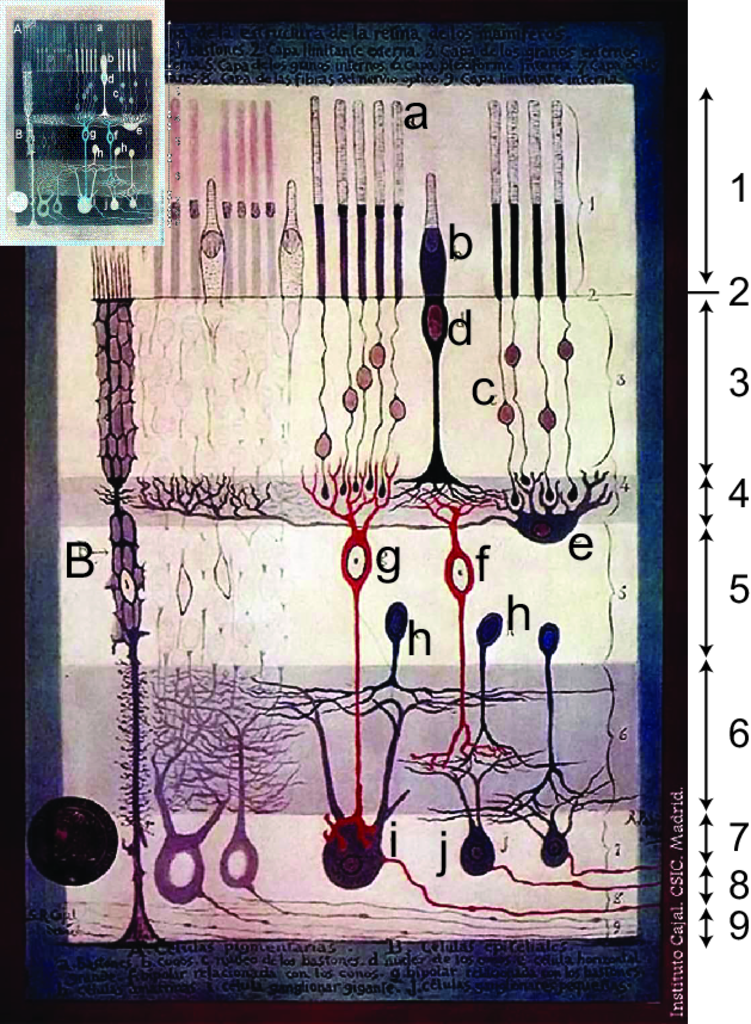
\includegraphics[width=.6\linewidth]{figures/taxonomy/cajal.eps}
    }
    \caption{Drawing of the retina by Santiago Ram\'{o}n y Cajal. In this drawing photoreceptors are in the top and light comes from the bottom:
    %(indeed, light needs to traverse all the layers of the retina before reaching the light sensitive layer). 
    1. Rod and cone layer. 2. External limiting membrane. 3. Outer granular layer. 4. Outer plexiform layer. 5. Inner granular layer. 6. Inner plexiform layer. 7. Ganglion cell layer. 8. Optic nerve fibre layer. 9. Internal limiting membrane. A. Pigmented cells. B. Epithelial cells. a. Rods. b. Cones. c. Rod nucleus. d. Cone nucleus. e. Large horizontal cell f. Cone-associated bipolar cell. g. Rod-associated bipolar cell. h. Amacrine cells. i. Giant ganglion cell. j. Small ganglion cells.
        %modified from \url{https://commons.wikimedia.org/wiki/File:Cajal_Retina.jpg}, originally 
        {\em Source}: ``Structure of the Mammalian Retina'' c.1900 By Santiago Ramon y Cajal.}
    \label{fig:cajal}
\end{figure}


The drawing of the retina (\fig{\ref{fig:cajal}}) shows the first layers of neurons that process the visual input. The retina is an amazing piece of the brain that transforms light into impulses. Light is first transformed into electric signal by the photoreceptors
\index{Photoreceptors}
(rods and cones) and is then processed by a few layers formed by several types of neurons (amacrine, bipolar, and ganglion cells). Finally, ganglion cells transmit the output of the retina through the optic nerve to the rest of the brain. The studies of Ram\'{o}n y Cajal revealed the circuitry of many parts of the brain but told us little about their functional behavior or how the circuits were processing information.

The {\bf retina}
\index{Retina}
was one of the first visual structures that was studied from a functional perspective. Haldan Keffer Hartline \cite{Hartline1938}, in 1938, using an innovative method to record the response of single optic nerve fibers (which corresponds to the axons of ganglion cells),
studied retinal ganglion cells and popularized the concept of {\bf receptive field}, previously introduced by Charles Scott Sherrington \cite{Sherrington1906} in 1906 when studying the tactile domain.

\marginnote{A review of how the concept of {\bf receptive field} evolved can be found in \cite{Spillmann2014ReceptiveFO}.}

The receptive field of a  neuron corresponds to the region of the input stimulus space (the retina in the case of a visual neuron) that has to be stimulated in order to produce a response in the neuron. Most neurons in the visual processing stream are activated only when light shines on a precise portion of the retina.

\marginnote{Only stimulation within the {\bf receptive field} (RF) of a neuron produces a response.
    \\[6pt]
    \centerline{
        \includegraphics[width=.4\linewidth]{figures/taxonomy/receptive_field.eps}
    }
}

Steven Kuffler (1953) studied the organization of the retina and showed that ganglion cells have concentric receptive fields with a circular {\bf center-surround organization} \cite{Kuffler1953}.
\index{Receptive field}
He did this by shining a small spot of light on different parts of the retina and recording the response of a ganglion cell as he changed the location of the spot of light. First Hartline, and then Kuffler, showed that there were two types of ganglion cells; a first group of cells, called {\bf on-center}, would get activated when the spot of light was inside a small region in the middle of the receptive field and would get deactivated (firing bellow their average rate) when the spot light was projected inside a ring around the center.
A second group had the opposite behavior, called {\bf off-center}. These results are fascinating because they reveal that the retina seems to be performing some sort of contrast enhancing operation (as we will discuss in other chapters) and their work motivated a large number of studies in {\bf computational neuroscience} and {\bf neuromorphic engineering} \cite{Mead89} that tried to reproduce the operations made in the retina. Haldan Keffer Hartline received the Nobel Prize in 1967 for his discoveries on how the eye processes visual information.


The axons of ganglion cells from both eyes projects to another structure called the {\bf lateral geniculate nucleus} (LGN). The LGN is composed of six layers of neurons and its output goes to the visual cortex and other visual areas. This structure receives inputs from both eyes but the signals are not mixed and the neurons in this area remain monocular. LGN neurons have concentric (center-surround) receptive fields. The role of the LGN is not completely understood but it may be involved in temporal decorrelation, attention modulation and saccadic suppression. Interestingly, only 5 percent of the input connections come from the retina while 95 percent of the LGN inputs are {\bf feedback connections} from the primary visual cortex and other areas.


Concentric receptive fields are very common in the early layers of visual processing, but things become more interesting when studying cells in the {\bf visual cortex}. One challenge was that the techniques used to record the responses of cells in the optic nerve could not be applied to record the activity of cells in the cortex. \Fig{\ref{fig:receptivefields}} shows some of the receptive fields found in the LGN. When a cell with an {\bf ON-center Receptive Field (RF)} is illuminated with a small spot of light projected on the inner part of the RF, the firing rate increases, as shown in \fig{\ref{fig:receptivefields}}{a}. The gray rectangle under the graph represents the duration of the stimulation. When the outer part of the RF is stimulated there is an inhibition of the cells response. \Fig{\ref{fig:receptivefields}}{a} shows an {\bf OFF-center RF}.


\begin{figure}[t]
    \centerline{
        \includegraphics[width=1\linewidth]{figures/taxonomy/receptive_fields.eps}
    }
    \caption{Receptive fields (RF) for retinal ganglion cells and oriented receptive fields from the primary visual system. (a) ON-center RF. (b) OFF-center RF. (c-d) Two types of oriented simple cell. (e) Sketch of the response of the cell from (c) to an oriented bar with different orientations in the center of its RF. The gray bar corresponds to the moment the bar is visible.}
    \label{fig:receptivefields}
\end{figure}

% https://www.cns.nyu.edu/~david/courses/perception/lecturenotes/ganglion/ganglion.html
Between 1955 and 1958, David H. Hubel invented a microelectrode that allowed him to record the activity of individual cells in the cortex. He then went to work with Torsten N. Wiesel in Kuffler's lab. They used Hubel's technique to record the response of cells in the visual cortex of cats; this work resulted in them receiving the Nobel prize in 1981.


% https://www.ncbi.nlm.nih.gov/pmc/articles/PMC1363130/pdf/jphysiol01298-0128.pdf

In 1959, Hubel and Wiesel published the study that marked the beginning in understanding how visual information is processed in the brain \cite{HubelWiesel59}. They studied 45 neurons for a period of two to nine hours from the striate cortex on an anesthetized cat. They exposed each neuron to a diverse set of visual stimuli containing spots of various sizes and locations, and {\bf oriented bars}. For most of the neurons they could locate a region of the retina that produced a firing of the neuron when stimulated with light. However, not all types of visual stimuli were effective in driving neurons at the cortical level. %In general, large circular spots of light were ineffective. 
% Original text: In most units it was possible to find a restricted area in the retina from which firing could be influenced by light. This area was called the receptive field of the cortical unit, applying the concept introduced by Hartline (1938) for retinal ganglion cells. 

Hubel and Wiesel discovered that some neurons in the visual cortex were best stimulated by an oriented bar at an specific orientation when it appeared at the center of the neuron's receptive field. They found different types of cells in the primary visual cortex, some that were similar to those found in the retina and LGN (center-surround), others selective to oriented bars, and more complex ones.
They classified each cell according to its attributes: spatial selectivity, orientation preference, eye preference (left or right), and the type (simple, complex, or hypercomplex).

\Fig{\ref{fig:receptivefields}}{c} shows an {\bf oriented simple cell}, while \fig{\ref{fig:receptivefields}}{d} shows another type of simple oriented cell found in the visual cortex. An oriented cell shows increased firing rate when stimulated with an oriented bar in the positive region of the RF with the preferred orientation.
\index{Visual cortex}

% https://www.cns.nyu.edu/~david/courses/perception/lecturenotes/V1/lgn-V1.html
\Fig{\ref{fig:visual_pathways}}
shows a schematic of the visual pathways from the retina up to the primary visual cortex.The first visual area in the visual cortex is called {\bf V1}. It is a sheet of neurons is arranged along several layers as shown in \fig{\ref{fig:visual_pathways}}. %Neurons in V1 are organized along {\bf columns} creating arrangements with nearby neurons having similar preferred orientations, with a smooth transition from one part of the visual cortex to another and with alternance in eye preference.  
Hubel and Wiesel found that neurons in V1 are organized along {\bf columns}. When probing with an electrode, as the electrode went from the surface to the bottom of V1, all the cells found were selective to the same orientation. When moving the electrode along one horizontal direction, they found that the preferred orientation changed smoothly (orientation columns), and when moving the electrode along the perpendicular horizontal direction, the cells changed the eye preference, alternating between the two eyes with some binocular cells between them (ocular dominance columns). A section of around 1 $\times$ 3 mm (called a {\bf hypercolumn})
\index{Hypercolumn}
covers all orientations and both eyes for a small portion of the visual field.

Margaret Livingston, in collaboration with David Hubel, discovered color sensitive neurons \cite{Livingstone1984AnatomyAP} organized in blobs surrounded by orientation-sensitive neurons in the visual cortex.
%% The schematic is just a sketch that should not be taken too seriously but it reflects the actual structural organization of the vision system. In biology, hardware and algorithm are tied together constraining each other.   ****** I don't feel this sentence adds anything--Bill.


\begin{figure}[t]
    \centerline{
        \includegraphics[width=.7\linewidth]{figures/taxonomy/visual_pathways_aina.eps}
    }
    \caption{Visual pathways. The retina projects the axons of the ganglion cells into the lateral geniculate nucleus (LGN). In each hemisphere, the LGN gets inputs from both eyes (the LGN on the right gets the right side of each retina, which corresponds to the left side of the visual field). The output of the LGN is divided into three channels; the parvocellular, magnocellural, and koniocellular (not shown). Those channels project into the primary visual cortex following a very regular architecture organized along hypercolumns. The koniocellular pathway projects into the color blobs in the upper layer of the visual cortex. Figure modified from \cite{kandel:neural}.}
    \label{fig:visual_pathways}
\end{figure}

\marginnote{Compare the drawing from \fig{\ref{fig:visual_pathways}} with the one made a thousand years earlier by Ibn al-Haytham, shown in \fig{\ref{fig:Alhacen}}.}


Cells in the visual cortex project their outputs to a diverse set of other visual areas following two main streams (the ventral stream and the dorsal stream) and project into specialized areas performing motion processing (area MT), face processing (fusiform face area [FFA]; see\cite{Kanwisher1997TheFF}), and object recognition (IT).

As a result of all those discoveries in neuroscience, a large community of interdisciplinary researchers developed models trying to explain the function of visual neurons. Many of the neurons in the early layer of visual processing (retina, LGN, and visual cortex) can be approximated by linear filters with rectifying nonlinearities and contrast control mechanisms, which are the basis of many computer vision algorithms as we will see throughout this book.


%``At the cortical level a circular spot was often ineffective; for best driving of each unit it was necessary to find a spot with a particular form and orientation."




%Face area

%Place cells

%Motion area

%Computational neuroscience
%A number of studies tried to 
%Color coding,
%Attick for the ganglion cells, retinal response
%Bruno, David: Cortex


\subsection{Marr's Computational Theory of Vision}


David’s Marr influential book \booktitle{Vision} was published posthumously in 1982 \cite{Marr82}.
%David Marr started as a
Marr’s philosophy was influenced by advances in computer vision, and studies in cognitive psychology and neurophysiology. Studies in psychology at the time suggested that visual information was processed by independent modules of perception, each one devoted to a specific task (stereo vision, motion perception, color processing), and that visual images were analyzed by independent spatial-frequency-tuned channels. Progress in neurophysiological experiments using single cell recordings showed a strong connection between perception and neural activity. In the 1970’s, computer vision was already a well-established field. Some of the advances that inspired Marr's philosophy were the work by David L. Waltz \cite{Waltz1972GeneratingSD} on the interpretation of block worlds, Edwin H. Land and John J. McCann’s Retinex theory about color perception \cite{Land1971}, and Berthold Horn’s theory of shape from shading \cite{Horn1977}, among many other works.

David Marr, together with Tomaso Poggio and others, postulated that it was important to separate the analysis of the task being solved from the particular mechanism used to solve it \cite{Marr82}. Marr said that the vision problem should be understood at different levels, and that what was missing in previous theories of vision was to understand vision as an {\bf information-processing task}. Marr proposed that an information-processing device should be described at three levels:

\begin{itemize}
    \item {\bf Computational theory}. This level of description should answer the following questions: what is the task to be perform and why should it be carried out? In the case of vision, the task is to derive properties of the world from images. This level of description should specify what the mapping is between the input and output, and why this mapping is appropriate for the task that the device needs to solve. This level does not specify how that mapping should be constructed or which algorithm will implement it.
    \item {\bf Representation}. We should define which representation will be used for the input and output. The representation is a system of making explicit certain types of information present on a signal. For instance, an image could be represented by the sequence of values that encode the color of each pixel, but it could be also represented using a Fourier decomposition. The choice of representation will make explicit certain type of information while hiding other information, which will become harder to access. The algorithm used to implement the mapping between input and output will be strongly dependent on the representation used. The importance of the choice of representation is very present in today’s computer vision community. Examples such as using position encoding to represent location illustrate the dramatic effect that the choice of representation and algorithm can have in the final system performance. We will discuss the importance of representations many times throughout this book.
    \item {\bf Hardware}. Finally, the representation and algorithm will have to be implemented in a physical device.
\end{itemize}

Marr noted that when trying to explain visual phenomena, one needs to find what is the right level to use to describe it. For instance, the trichromatic color theory of human perception is explained by the hardware level (i.e., by the three color receptors in our retina) while the bistable nature of the Necker cube is likely to be related to the 3D representation. The illusions shown in \fig{\ref{fig:measuringScene}}, are also likely due to the representation and algorithm used and they are rather independent on the particular hardware implementation. Marr considered that Gibson was asking the right questions, getting very close to a computational theory of vision, but that he had a naive view on how difficult it would be to solve them. We will return to this point in \chap{\ref{chapter:simplesystem}} when we will build a simple visual system.


\begin{figure}[t]
    \centerline{
        \includegraphics[width=.9\linewidth]{figures/taxonomy/necker.eps}
    }
    \caption{Necker cube illusion, introduced by Louis Albert Necker \cite{Necker1832}. Figure recreated from \cite{Marr82}.}
    \label{fig:necker_cube}
\end{figure}


Marr postulated that these three levels of understanding can be studied relatively independently, despite their loose coupling, with
each problem needing description at the appropriate level. This message, although simple, sometimes is often ignored in today’s computer vision where the task being solved is tightly connected to an architecture (usually a neural net) without a clear understanding of what is being computed, what the representations mean, or how something is being solved.


In David Marr’s approach, vision was implemented as a sequence of representations, starting from the image represented as a sequence of pixel intensities, and then transforming each representation into another one that extracts more explicit information about the geometry and objects present in the world. The sequence of representations proposed by Marr was the following:

\begin{itemize}
    \item Image: The collection of pixel intensities.
    \item Primal sketch: Represents changes in the image (edges, junctions, zero-crossings) and their spatial organization.
    \item 2.5D sketch: Contains an estimation of the distance between the observer and the visible surfaces in the world at each pixel, also called a {\bf depth map}. It also contains information about depth discontinuities and surface orientations.
    \item 3D model representation: Objects are represented as 3D shapes together with their spatial organization.
\end{itemize}

\marginnote{You will notice a strong parallelism between the sequence of representations proposed by Marr and the particular algorithm that we will discuss in \chap{\ref{chapter:simplesystem}} when building the simple visual system.}

\Fig{\ref{fig:sketch}} shows the image of a cube, and its
%2$\sfrac{1}{2}$-D 
2.5D
sketch as proposed by Marr \cite{Marr82}. The arrows ({\bf gauge-figures}) represent surface orientation. The dashed lines are surface orientation discontinuities and the black lines are occlusion boundaries. The pixel intensities represent distance between the observer and the visible surfaces of the cube. Depth is represented by gray levels. Intensity increases with depth.




\begin{figure}[t]
    \centerline{
        \includegraphics[width=.9\linewidth]{figures/taxonomy/sketch.eps}
    }
    \caption{Image of a cube, and its
        %2$\sfrac{1}{2}$-D 
        2.5D
        sketch. Figure inspired from figure 4-2 from \cite{Marr82}.}
    \label{fig:sketch}
\end{figure}



It is hard to overstate the influence that Marr’s book had in shaping the thinking of several generations of computer vision scientists, directly or indirectly.
Perhaps Marr's shortcoming was underestimating the role of learning in constructing representations. A learning-based architecture could
determine the sequence of representations that lead to the desired behavior, which is the premise of deep learning.  Current approaches specify vision tasks in terms on training and test sets, loss function, representation, architecture, and optimization as we will discuss later.


%\subsection{Treismann's feature integration theory}

\subsection{Computer Vision}

%\reviewcomment{Missing references.}

Computer vision has become an exciting and fast evolving area of research. We believe it is important to understand the field of computer vision within the scientific context that has been laid out in the previous sections. Computer vision is not just an engineering discipline that tries to build systems that see. Instead computer vision is another aspect of the interdisciplinary scientific quest that has focused on understanding how natural intelligence and perception works.

Doing a review of the field of computer vision and being fair to all of the people that have contributed to the field in a short subsection such as this one is not a reasonable task. It has the challenge that recent history is difficult to summarize as it requires fine-grained temporal resolution, and in many cases, we lack the perspective to identify the crucial discoveries. We will include those references throughout the book and we will just paint here, with a few coarse strokes, the main directions in the field.

%Tom Binford 

In 1963, at MIT, Larry Roberts became the first computer vision Ph. D. entitled \booktitle{Machine Perception of Three-dimensional Solids} \cite{Roberts63}.
% https://dspace.mit.edu/bitstream/handle/1721.1/11589/33959125-MIT.pdf?sequence=2
\marginnote{Larry Roberts did his Ph.D. under the supervision of Peter Elias, and expert in the field of information theory that introduced convolutional codes, a type of error-correcting code, still in use in communication systems.}[-1in]

The period of 1960--1990 was dominated by the geometric perspective of computer vision and included concepts such as stereo vision \cite{Longuet-Higgens1981}, shape from shading \cite{Horn89a}, multiview geometry \cite{Faugeras93,Hartley2004}, motion estimation \cite{Horn81}, and model driven object recognition \cite{Fischler1973,Mundy2006}. These methods transformed old hypothesis into concrete algorithms capable of extracting information from images. During this period there were also many advances in building image representations such as edge-based representations \cite{Canny86,Harris88,Koenderink88c,Perona90b}, filter-based image pyramids \cite{Granlund78,Burt83,Koenderink87,Malik90,Freeman91}, and Thomas O. Binford's generalized cylinders for 3D object representation \cite{binford1971}, as well as rule-based vision systems.

The decade of 1990--2000 experienced an acceleration of computer vision, in part because digital cameras became common. There was a change toward measuring ecological image properties \cite{Gibson1979}, shifting away from rigid model-driven approaches, and focusing on human-driven perceptual properties such as image segmentation \cite{Shi00}, and texture modeling \cite{Bergen88,Malik90}. Object detection using learning-based approaches started gaining attention and there were significant advances in face detection \cite{Rowley1996,Leung1995,Moghaddam97}. The field of computer vision got broken into specialized subareas targeting different tasks and grew with a strong solid foundation based on first principles.


The decade of 2000--2010 focused on image classification and object recognition \cite{Viola01,Fergus07,Dalal2005,Felzenszwalb2010} and the creation of medium size benchmarks, with tens of thousands of images, started driving progress (Caltech 101 \cite{caltech101}, PASCAL \cite{Everingham2010}, LabelMe \cite{Russell2008}, CIFAR \cite{cifar100}). The introduction of benchmarks popularized new metrics and guidelines for reproducible research in the field. There was an explosion of image descriptors (BoW \cite{Csurka2004}, SIFT \cite{Lowe04}, HOG \cite{Dalal2005}, GIST \cite{oliva01}) that, combined with machine learning (decision trees \cite{Lepetit2006}, boosting \cite{Tieu00}, support vector machines, and graphical models and belief propagation), provided the basis to address many vision tasks. The first very large image databases, with millions of images, (Tiny Images \cite{torralba2008}, ImageNet \cite{russakovsky2015imagenet}, COCO \cite{lin2014microsoft}) appeared with the hypothesis that most of the tasks on vision need to be learned. Although learning played an important role, most of the computer vision architectures and features were designed manually.

\marginnote{
    Some example images from the COIL dataset \cite{Nene1996}:
    \\[6pt]
    \centerline{
        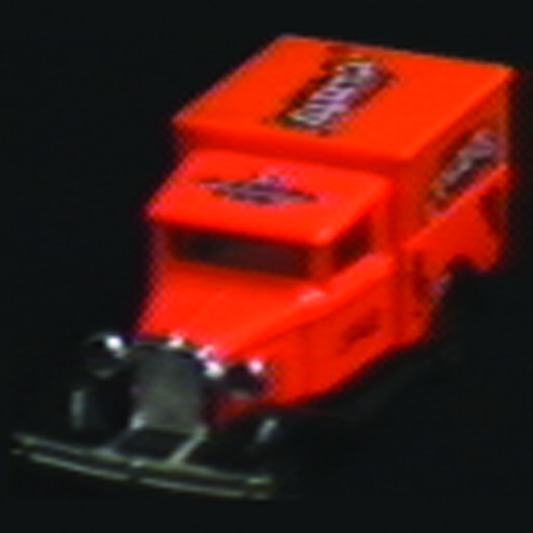
\includegraphics[width=0.2\linewidth]{figures/taxonomy/obj100__295.jpg}
        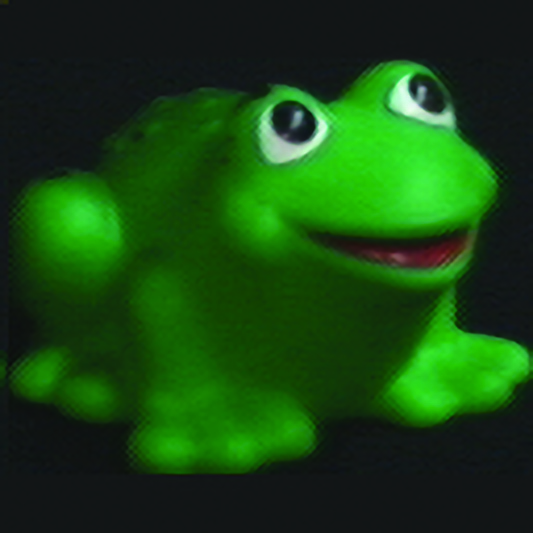
\includegraphics[width=0.2\linewidth]{figures/taxonomy/obj28__240.jpg}
        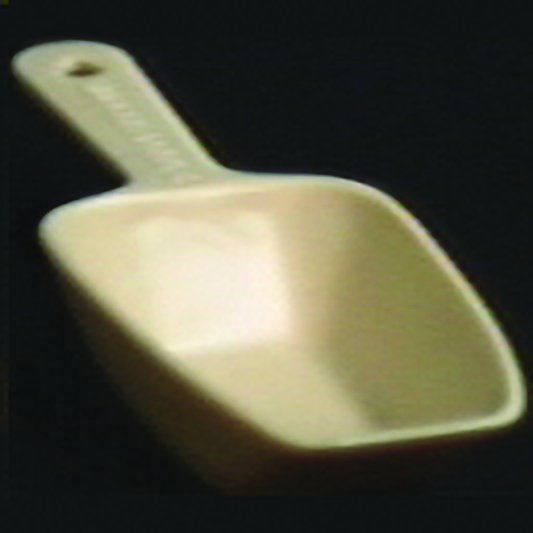
\includegraphics[width=0.2\linewidth]{figures/taxonomy/obj44__255.jpg}
        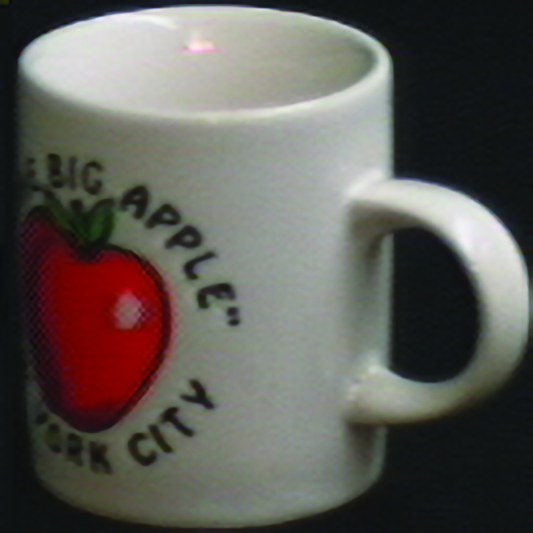
\includegraphics[width=0.2\linewidth]{figures/taxonomy/obj45__35.jpg}
    }
}

The decade of 2010--2020 has been clearly dominated by learning-based methods using deep learning as the main framework in all areas of computer vision.

\subsection{Learning-Based Vision}

%\reviewcomment{Unfinished. Text incomplete and missing references.}


While many previous perspectives on perception began with models about how perception might
work, learning-based approaches take a different path. They rely on flexible architectures that incorporate as few hypothesis about perception as possible, and instead focus on data to learn to build the right model for perception.

Learning-based vision has its roots in the philosophical tradition of empiricism, which holds that knowledge about the world should be acquired by experience, rather than solely through reason (an approach known as rationalism). The modern day term for experience is ``data,'' and learning is really all about data.



Learning derives vision algorithms by fitting functions to data. One way to think about it is that our goal is to ``program'' a vision algorithm and there are a few ways to do so (\fig{\ref{fig:taxonomy:programming_vs_learning}}). One way is to write the algorithm directly in Python code: first we will compare the intensity of this pixel and that pixel, then we will threshold about some such value, and so on. Another approach is to derive the algorithm as the rational thing to do given some underlying model of the world, for example, because overlapping objects generically produce contrast edges in the image, the optimal way to detect boundaries between objects is to look for such and such particular kind of contrast. The third approach --- the learning approach --- is to program algorithms via data: first collect a bunch of examples of inputs and the correct output, then fit a function that replicates these exemplar mappings from input to output.


\begin{figure}[t]
    \centerline{
        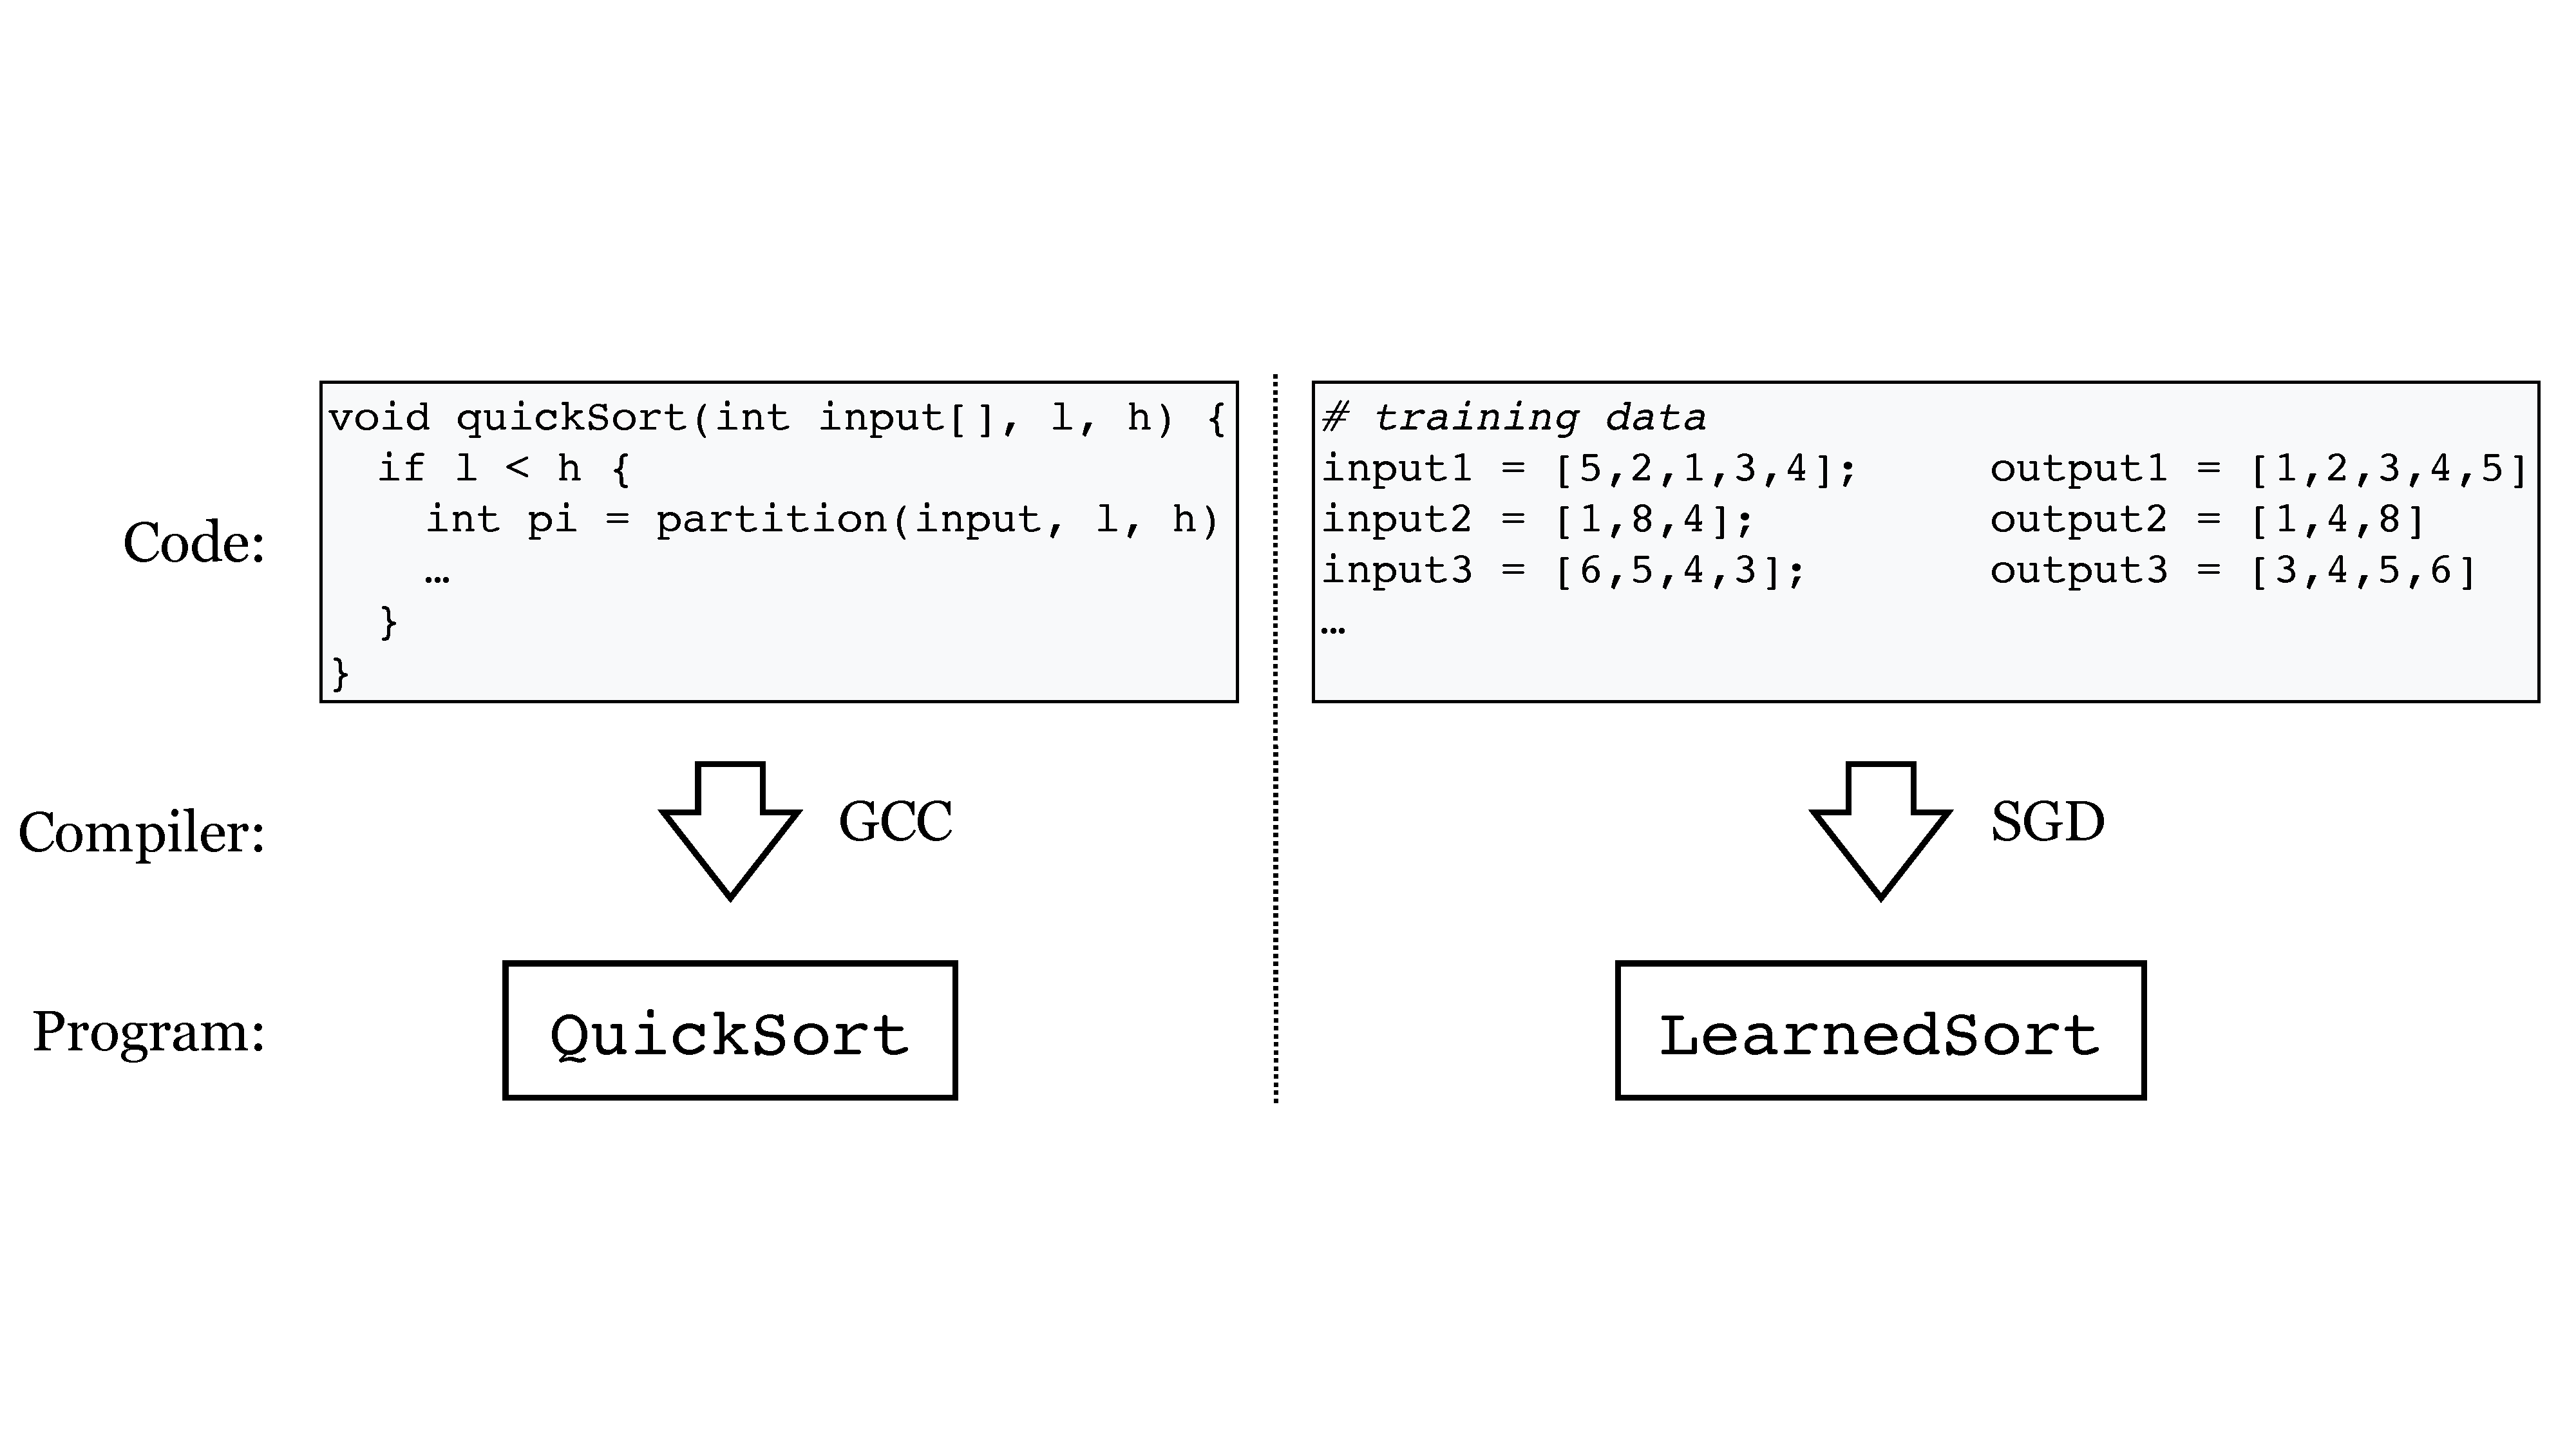
\includegraphics[width=1\linewidth]{figures/taxonomy/programming_vs_learning.pdf}
    }
    \caption{Two ways of programming an algorithm. Left: traditional way, Right: the machine learning way. You will learn about the machine learning ``compiler'', called Stochastic Gradient Descent (SGD), in \chap{\ref{chapter:backpropagation}}.}
    \label{fig:taxonomy:programming_vs_learning}
\end{figure}


Learning algorithms have been a part of computer vision since the field's origins. In 1958, Frank Rosenblatt published one of the first formal learning algorithms, called the {\bf perceptron}\index{Perceptron}
learning algorithm, and showed that it can, in principle, learn to recognize certain simple visual patterns~\cite{rosenblatt1958perceptron}.
The perceptron was also one of the first artificial neural nets, a computational model of biological brains. The ability of perceptrons to learn to solve recognition problems created an explosion of interest in neural nets.

\marginnote{
    Rosenblatt published the perceptron algorithm in the journal \booktitle{Psychological Review} in 1958. This is a nice example of the interdisciplinary nature of the AI field in its origins.
}

Interest in neural nets has since gone through a series of ebbs and flows (\fig{\ref{fig:taxonomy:neural_net_enthusiam}}). Note that these cycles have partially lined up with interest in learning algorithms more generally, but there have also been phases where interest in neural nets was low but interest in other learning algorithms was high.

\begin{figure}[t]
    \centerline{
        \includegraphics[width=0.7\linewidth]{figures/taxonomy/neural_net_enthusiasm.eps}
    }
    \caption{Enthusiasm for neural nets has gone up and down over time, with a period of roughly 25 years. What will happen next?}
    \label{fig:taxonomy:neural_net_enthusiam}
\end{figure}


In 1969, Marvin Minsky and Seymour Papert published a book titled \booktitle{Perceptrons: an introduction to computational geometry}~\cite{marvin1969perceptrons}. You might think this would be a book that would increase the excitement around perceptrons, but in fact it largely killed it. Minsky and Papert showed that perceptrons are incapable of learning basic logical operations. Clearly then, perceptrons could not be the basis of intelligence.

It wasn't until the 1980s that interest in learning algorithms, and neural nets in particular, began to surge again. The reason was because researchers showed that perceptrons could be stacked to create systems capable of complex operations, including logic. These systems were the precursors to the {\bf deep learning} systems that are dominate today. In this decade, several architectures specific to vision were also introduced, including Kunihiko Fukushima's \booktitle{neocognitron}\index{Neocognitron}, which was a precursor to modern convolutional neural networks~\cite{fukushima1980neocognitron}. In 1989, Yann LeCun et al. showed how these kinds of networks can be efficiently trained \cite{lecun1989backpropagation} and their system was put into use for recognizing handwritten digits by the US Postal Service.


One of the peaks of neural network research in the 1980s was the publication of \booktitle{Parallel Distributed Processing} by David Rumelhart and Jay McClelland~\cite{Rumelhart86}. This book mixed the neuroscience of the brain with computational models of distributed processing in artificial networks.

\marginnote{\booktitle{Parallel Distributed Processing}~\cite{Rumelhart86} cover:
    \\[6pt]
    \centerline{
        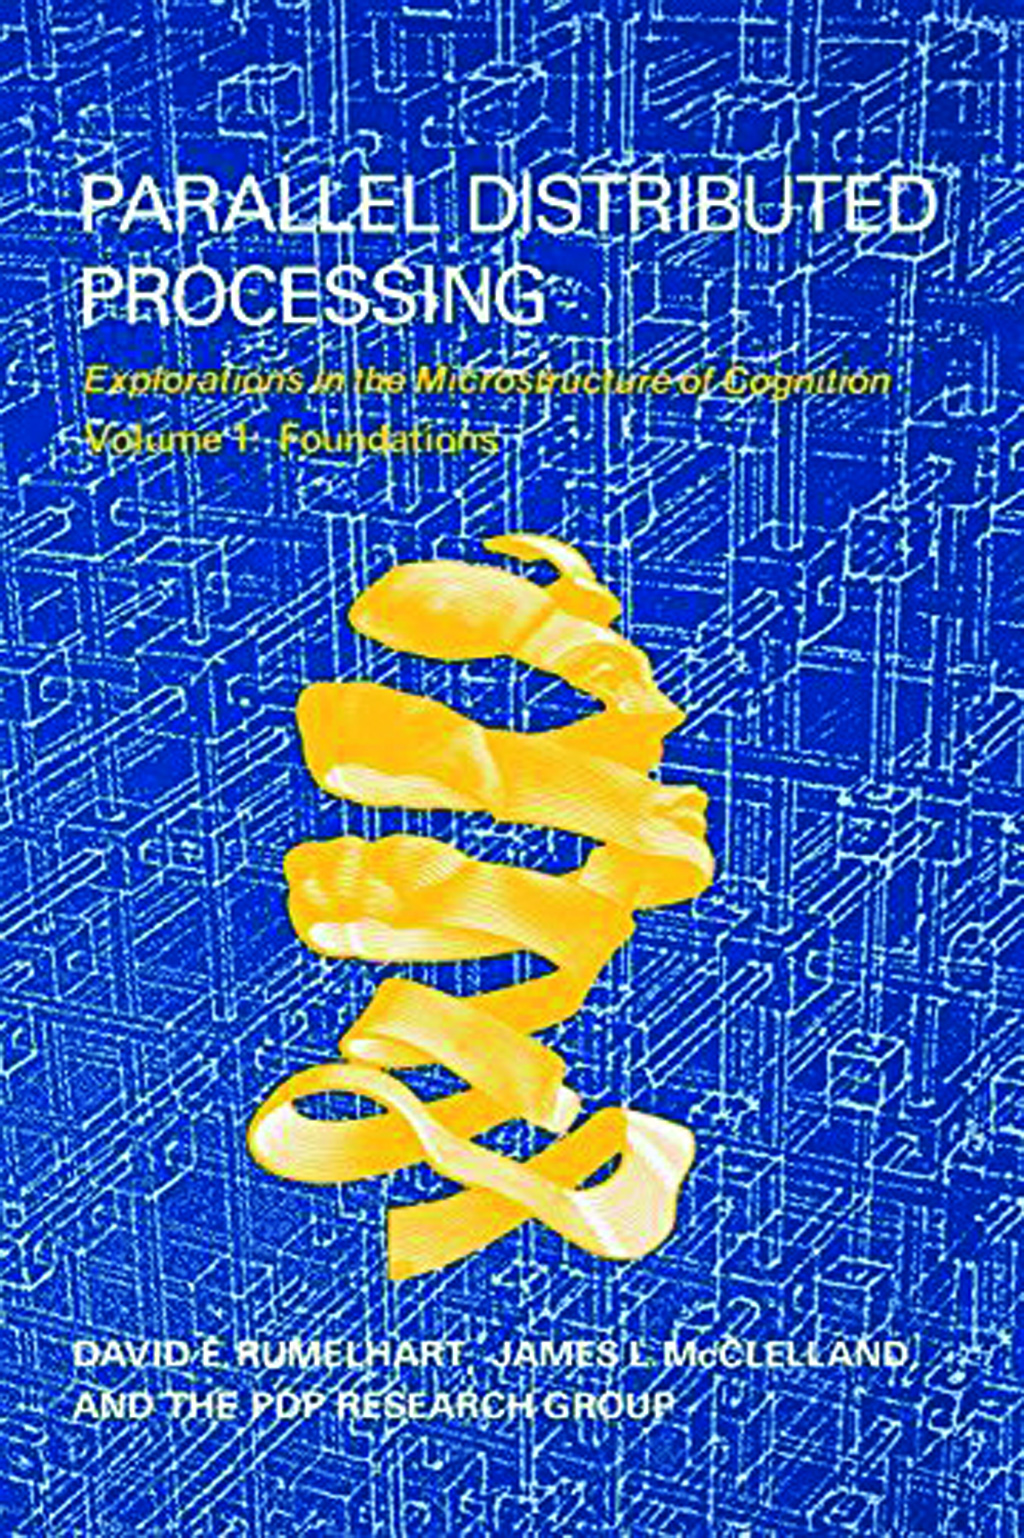
\includegraphics[width=.35\linewidth]{figures/taxonomy/pdp_cover.jpg}}
}[-.8in]

Unfortunately, however, at that time we did not have the compute and data necessary to make these systems really work, and interest waned during the 1990s. By the year 2000, the field of AI as a whole was firmly in a ``winter''; the promises of the 1980s had failed to materialize and the study of learning algorithms continued on without much fanfare in just a few corners of academia. Nonetheless, several major advances did occur in the relative quiet of the 1990s and early 2000s.
For example, in 2001, Paul Viola and Michael Jones published a method that used a simple learning algorithm called {\bf boosting} to detect faces in photos~\cite{Viola01}.
\marginnote{Face detection example from \cite{Viola01}:
    \\[6pt]
    \centerline{
        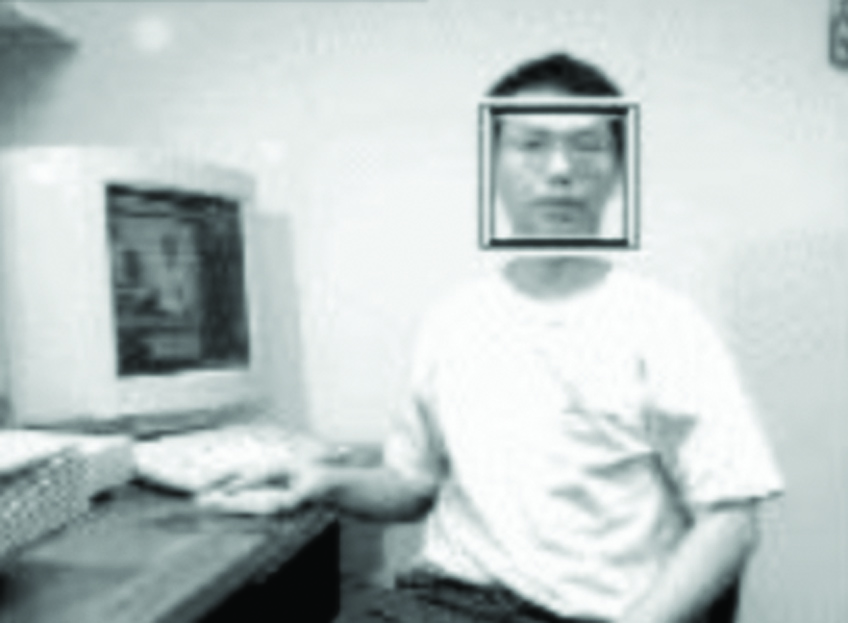
\includegraphics[width=.4\linewidth]{figures/taxonomy/viola_jones_example.jpg}}
}[-1.25in]
This method outperformed the complicated hand-engineered face detectors of the time in terms of computational efficiency and detection rate, and even became a popular algorithm used in consumer cameras.



The 2000s were a decade where learning returned to the foreground. One common pattern was to take the best hand-engineered features and feed them as input to a shallow learning machine, such as a support vector machine~\cite{cortes1995support}. Gradually more and more of the vision pipeline was replaced with learned modules. Finally, in 2012, a deep neural net called AlexNet dramatically outperformed all existing methods for image classification, and did so with a system that used learning \textbf{end-to-end} (for each processing stage from the input pixels to the output predictions)~\cite{krizhevsky2012imagenet}. This event has come to be called the ``ImageNet Moment'' since AlexNet's dramatic performance was first demonstrated at the 2012 ImageNet competition~\cite{russakovsky2015imagenet}.
\marginnote{WordNet is an electronic dictionary used to define word hierarchies \cite{Fellbaum1998}:
    \\[6pt]
    \centerline{
        \includegraphics[width=.4\linewidth]{figures/taxonomy/exampleTree12.eps}
    }
}[-.8in]
The ImageNet moment was a watershed for learning-based vision and for neural networks. In the few years after 2012, learning became the key ingredient in almost all research on computer vision. As of the 2020s, it is hard to find any computer vision system that does not use deep learning somewhere in its pipeline.

It may seem like learning-based vision is very different than other approaches, but actually it is similar in many ways. The study of vision consists of the structure of the input, the structure of the output, and the mapping between the two. Learning-based vision does not fundamentally change any of these: the input and target output are the same as before, and the mapping is remarkably similar as in other approaches. The big difference with learning-based vision is how you \textit{find} the mapping. In this sense, learners are just like a new kind of vision scientist: they play the same role as the humans who, in previous eras, sat down and thought deeply to determine the way vision works.


%-- let the data determine the solution -- which stands in contrast to philosophical schools based on logic / deduction.


%Learning-based vision is actually not so different than other approaches, except that the vision algorithms are ``programmed" by a machine learner rather than by a human. 
In this book we will see that very often machine learners come up with similar vision algorithms as were previously designed by humans. But in many ways machine learners are also more powerful than human designers, and machine learned algorithms have now far exceeded those designed by humans in terms of raw performance.



%1980 - Kunihiko Fukushima; neocognitron

%2001 - Viola and Jones

%2012 - deep learning


%the communities in cognition, neuroscience and computer vision got separated 

%Graph of enthusiam for neural nets over time.


%There is now a trend into building general vision systems 

%And hopefully soon, the areas of cognition, neuroscience and computer vision will work together again to advance our understanding of natural and artificial intelligence. 


%Do the learning approaches overestimate the importance of learning and undervalue the importance of model-driven representations? 



\section{What's Next?}


In a span of more than 2000 years, from the Greeks' extramission theories of vision to the understanding of the neural mechanisms and the engineering of computer vision systems, we have come a long way in our understanding of the nature of perception.
Each step during the evolution of vision theories revealed important aspects of perception ignored by the previous theories. What theories will come next? What is missing now? Certainly, many things. For instance, we are missing visual common sense (now powered by large language models), integration with other perceptual systems, and, most importantly, a theory of embodied perception. And those are just the most obvious. There might be many other steps missing that we are not smart enough to see from where we are standing right now.



\section{Concluding Remarks}

The goal of this chapter was to define the topic of computer vision by placing it inside its historical context. We believe that any researcher of computer vision would benefit by studying vision from an interdisciplinary perspective as it will provide a solid basis for creativity, technical depth, and an understanding of its societal impact. We hope this chapter also inspires students to learn more about this fascinating field and to get excited by its potential.


 % PHILLIP & ANTONIO



%%%%%%%%%%%%%%%%%%%%%%%%%%%%%%%%%%%%%%%%%%%%%%%%%%%%%%%%%
% 1.Introduction
\include{parts/part_foundations}

    %\ifx\isEmbedded\undefined
%	% Loading common settings
%	\input{macros/common}
%	% Loading common variable definitions 
%	\input{macros/macros}
%	\begin{document} 
%\else
%\fi
%



%\setcounter{chapter}{1}

\chapter{A Simple Vision System}
\label{chapter:simplesystem}

\section{Introduction}

The goal of this chapter is to embrace the optimism of the 1960s and to hand-design an end-to-end visual system. During this process, we will cover some of the main concepts that will be developed in the rest of the book. 


In 1966, Seymour Papert wrote a proposal for building a vision system as a summer project \cite{Papert66}. The abstract of the proposal starts by stating a simple goal: ``The summer vision project is an attempt to use our summer workers effectively in the construction of a significant part of a visual system.'' The report then continues dividing all the tasks (most of which also are common parts of modern computer vision approaches) among a group of MIT students. This project was a reflection of the optimism existing in the early days of computer vision. However, the task proved to be harder than anybody expected.  

In this first chapter, we will discuss several of the main topics that we will cover in this book. We will do this in the framework of a real, although a bit artificial, vision problem. Vision has many different goals (e.g., object recognition, scene interpretation, three-dimensional [3D] interpretation), but in this chapter we're just focusing on the task of 3D interpretation.

\section{A Simple World: The Blocks World}


As the visual world is too complex, we will start by simplifying it enough that we will be able to build a simple visual system right away. This was the strategy used by some of the first scene interpretation systems.  Larry G. Roberts \cite{Roberts63} introduced the {\bf Block world}, a world composed of simple 3D geometrical figures. 
\index{Block world}
\marginnote{Blocks world from Larry Roberts' Ph.D. in June 1963.
\\[6pt]
\centerline{
\setlength{\fboxsep}{0pt}
\fbox{\includegraphics[width=.4\linewidth]{figures/simplesystem/roberts_phd_figure.eps}}
} 
}

For the purposes of this chapter, let's think of a world composed of a very simple (yet varied) set of objects. These simple objects are composed of flat surfaces that can be horizontal or vertical. These objects will be resting on a white horizontal ground plane. We can build these objects by cutting, folding, and gluing together some pieces of colored paper as shown in \fig{\ref{fig:simpleObjects}}. Here, we will not assume that we know the exact geometry of these objects in advance. 

\begin{figure}[t]
\centerline{
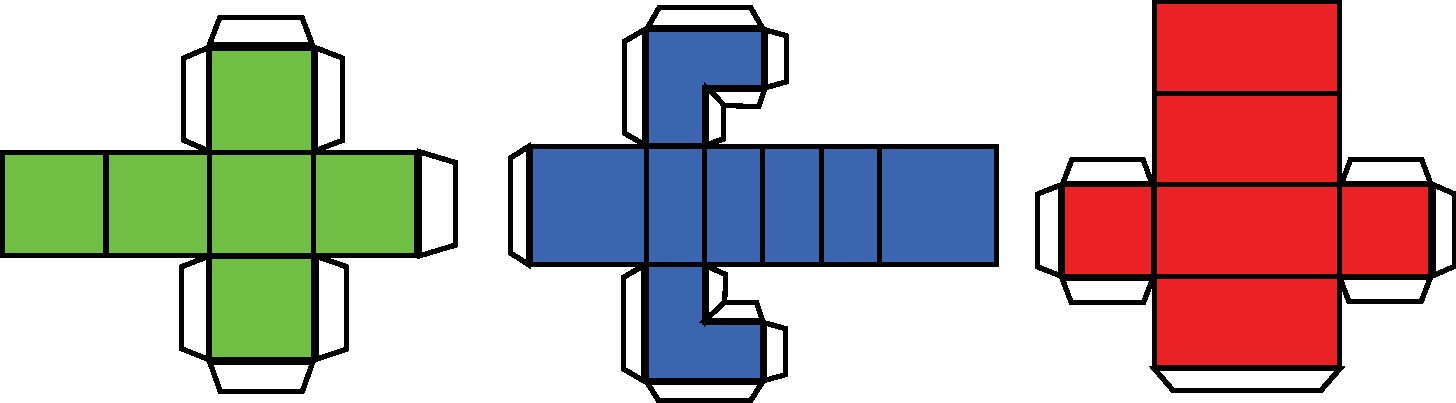
\includegraphics[width=1\linewidth]{figures/simplesystem/simpleObjects.pdf}
} 
\caption{A world of simple objects. Print, cut, and build your own blocks world!} 
\label{fig:simpleObjects}
\end{figure}



\section{A Simple Image Formation Model}

One of the simplest forms of projection is {\bf parallel} (or {\bf orthographic}) {\bf projection}\index{Parallel projection}. In this image formation model, the light rays travel parallel to each other and perpendicular to the camera plane. This type of projection produces images in which objects do not change size as they move closer or farther from the camera, and parallel lines in 3D remain  parallel in the 2D image.  This is different from the perspective projection, to be discussed in \sect{\ref{sec:pinhole_camera_formation}}, where the image is formed by the convergence of the light rays into a single point (focal point). If we do not take special care, most pictures taken with a camera will be better described by {\bf perspective projection}\index{Perspective projection}, as shown in \fig{\ref{fig:parallelProjection}}{a}.  


\begin{figure}[t]
\centerline{
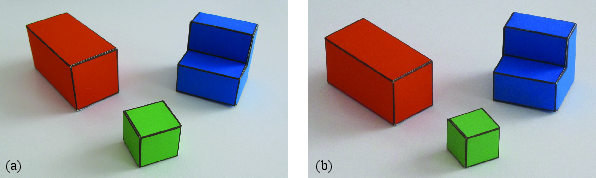
\includegraphics[width=1\linewidth]{figures/simplesystem/parallelProjection.pdf}
} 
\caption{(a) Close up picture without zoom. Note that near edges are larger than far edges, and parallel lines in 3D are not parallel. (b) Picture taken from far away using zoom resulting in an image that can be described by parallel projection.} 
\label{fig:parallelProjection}
\end{figure}

One way of generating images that can be described by parallel projection is to use the camera zoom. If we increase the distance between the camera and the object while zooming, we can keep the same approximate image size of the objects, but with reduced perspective effects, as shown in \fig{\ref{fig:parallelProjection}}{b}. Note how, in \fig{\ref{fig:parallelProjection}}{b}, 3D parallel lines in the world are almost parallel in the image (some weak perspective effects remain). 
\marginnote{Changing the zoom to compensate a moving camera can be used to create movie effects. This method was introduced by Alfred Hitchcock to create a sequence, centered in a subject, where the background moves away or closer to the subject.}[-.1in]


The first step is to characterize how a point in world coordinates $(X,Y,Z)$ projects into the image plane. \Fig{\ref{fig:projection}}{a} shows our parameterization of the world and the camera coordinate systems. The camera center is inside the 3D plane $X=0$, and the horizontal axis of the camera ($x$) is parallel to the ground plane ($Y=0$). The camera is tilted so that the line connecting the origin of the world coordinates system and the image center is perpendicular to the image plane. The angle $\theta$ is the angle between this line and the $Z$-axis. The image is parameterized by coordinates $(x,y)$. 

\begin{figure}[t]
\centerline{
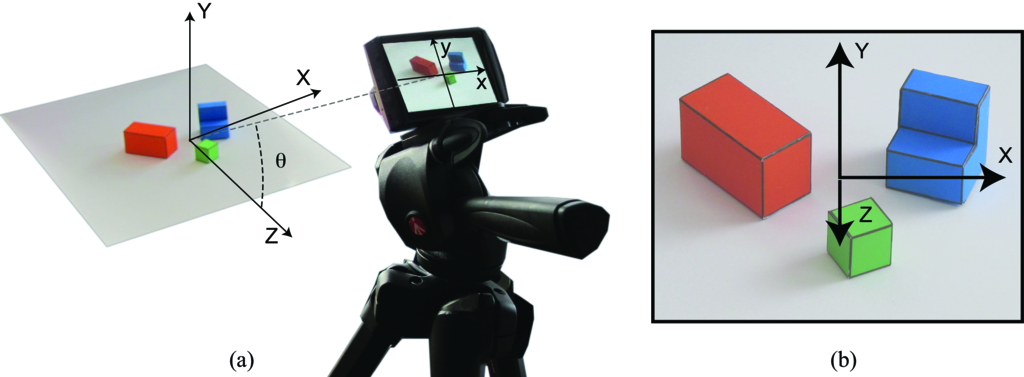
\includegraphics[width=1\linewidth]{figures/simplesystem/projection2.eps}
} 
\caption{A simple projection model. (a) World axis and camera plane. (b) Visualization of the world axis projected into the camera plane with parallel projection. The $Z$-axis is identical to the $Y$-axis up to a sign change and a scaling.} 
\label{fig:projection}
\end{figure}

In this simple projection model, the origin of the world coordinates projects on the origin of the image coordinates. Therefore, the world point $(0,0,0)$ projects into $(0,0)$.
%The center of the image is at coordinates $(x_0, y_0)$. 
The resolution of the image (the number of pixels) will also affect the transformation from world coordinates to image coordinates via a constant factor $\alpha$ (for now we assume that pixels are square and we will see a more general form in \sect{\ref{sec:camera_parameters}}) and that this constant is $\alpha=1$. Taking into account all these assumptions, the transformation between world coordinates and image coordinates can be written as follows: 
\begin{eqnarray}
x &=& X \\
y &=&  \cos(\theta) Y - \sin(\theta) Z 
% &=& \alpha X + x_0\\
%y &=& \alpha( \cos(\theta) Y - \sin(\theta) Z ) + y_0
\label{eq:projection}
\end{eqnarray}




With this particular parametrization of the world and camera coordinate systems, the world coordinates $Y$ and $Z$ are mixed after projection.  From the camera, a point moving parallel to the $Z$-axis will be indistinguishable from a point moving parallel to the $Y$-axis.


\section{A Simple Goal}

Part of the simplification of the vision problem resides in simplifying its goals. In this chapter we will focus on recovering the world coordinates of all the pixels seen by the camera. 

Besides recovering the 3D structure of the scene, there are many other possible goals that we will not consider in this chapter. For instance, one goal (which might seem simpler but is not) is to recover the actual color of the surface seen by each pixel $(x,y)$. This will require discounting for illumination effects as the color of the pixel is a combination of the surface albedo and illumination (color of the light sources and interreflections). 


\section{From Images to Edges and Useful Features}
\label{sec:algo_simple_world}


The observed image is a function, 
\begin{equation}
\img(x,y) 
\end{equation}
that takes as input location, $(x,y)$, and it outputs the intensity at that location. In this {\bf representation}, the image is an array of intensity values (color values) indexed by location (\fig{\ref{fig:imageAsSurface}}). 


\begin{figure}[t]
\centerline{
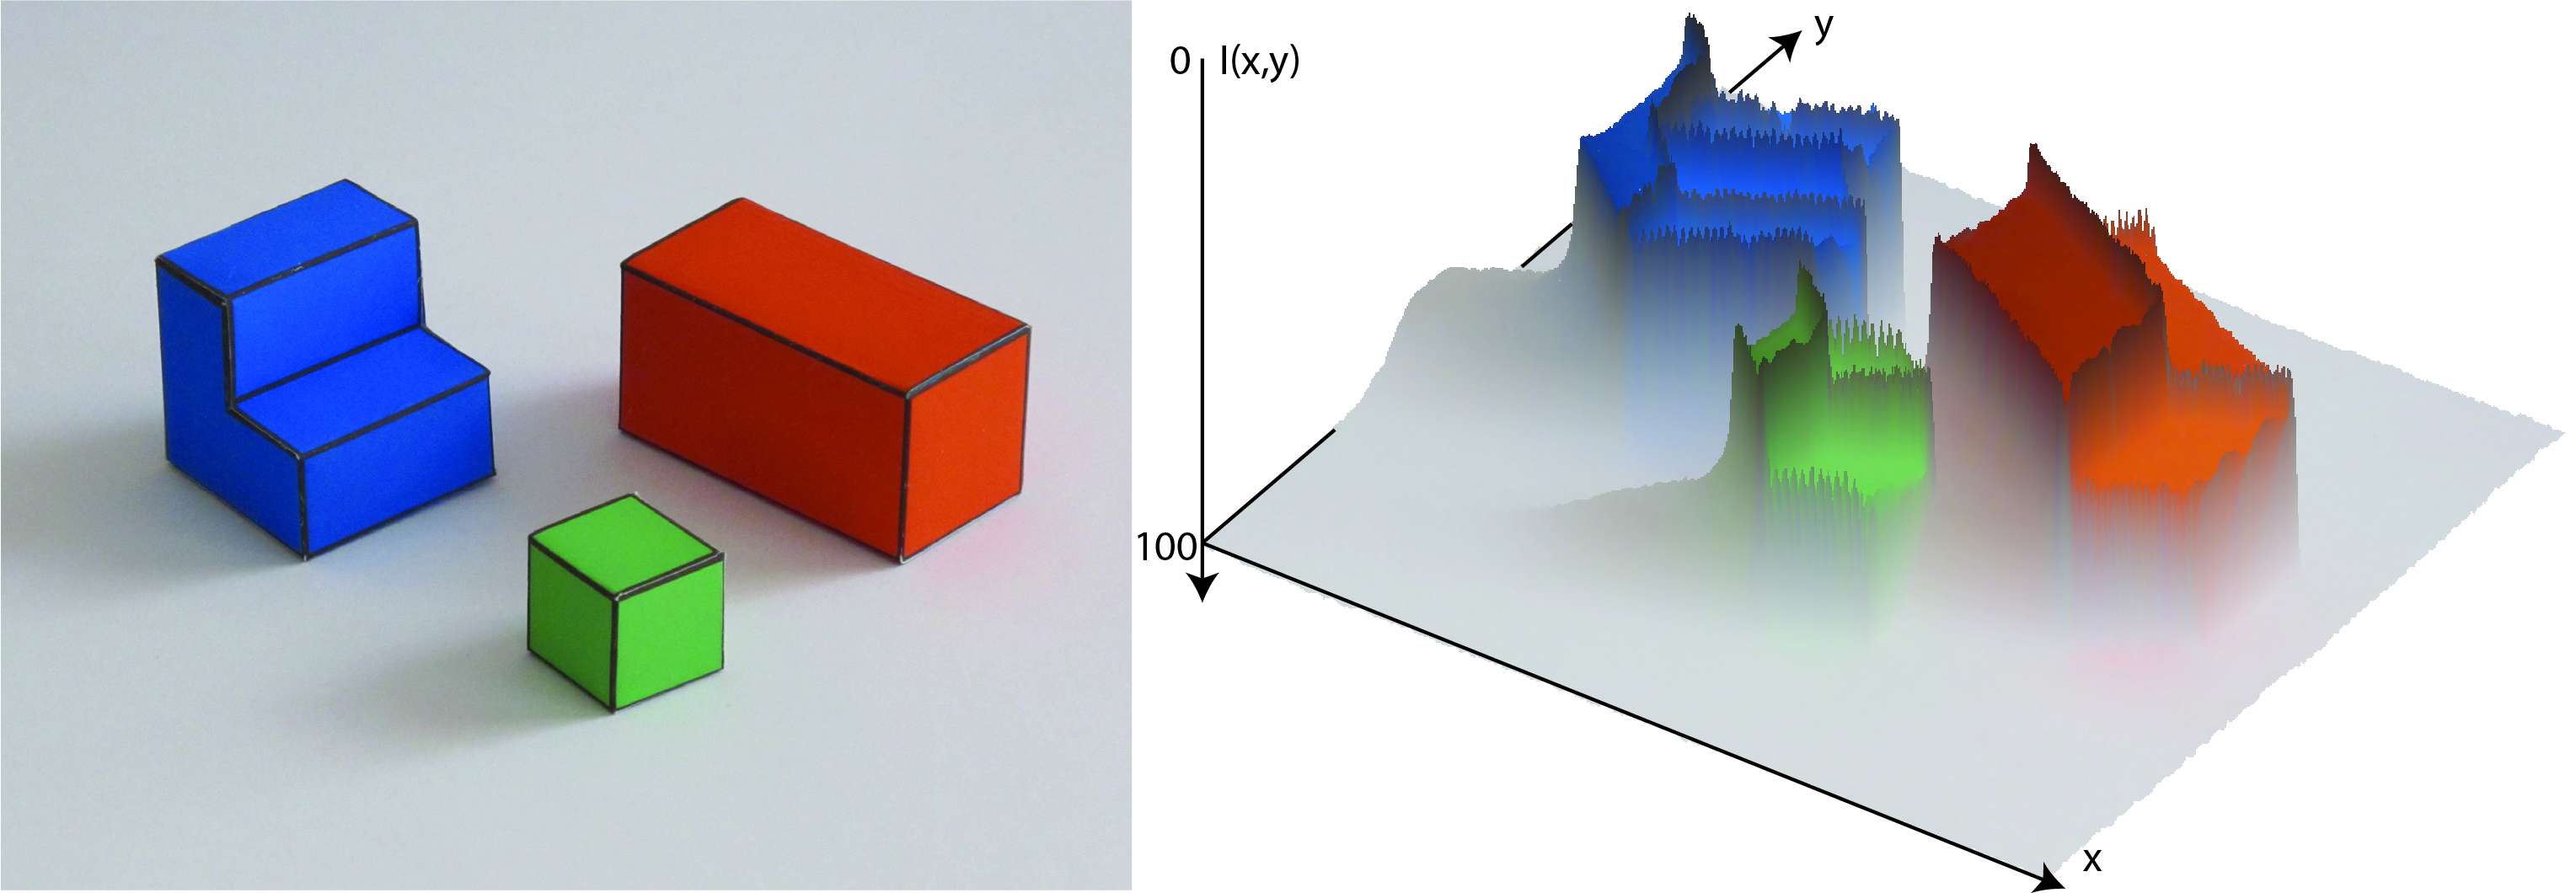
\includegraphics[width=1\linewidth]{figures/simplesystem/imageAsSurface.jpg}
} 
\caption{Image as a surface. The vertical axis corresponds to image intensity. For clarity here, we have reversed the vertical axis. Dark values are shown higher than lighter values.} 
\label{fig:imageAsSurface}
\end{figure}

%This representation is great if we are interested in knowing the light intensity coming from each direction of the space and striking the camera plane, as this information is explicitly represented. 
This representation is ideal for determining the light intensity originating from different directions in space and striking the camera plane, as it provides explicit representation of this information. The array of pixel intensities, $\img(x,y)$, is a reasonable representation as input to the early stages of visual processing because, although we do not know the distance of surfaces in the world, the direction of each light ray in the world is well defined. However, other initial representations could be used by the visual system (e.g., images could be coded in the Fourier domain, or pixels could combine light coming in different directions). 


However, in the simple visual system of this chapter we are interested in interpreting the 3D structure of the scene and the objects within. Therefore, it will be useful to transform the image into a representation that makes more explicit some of the important parts of the image that carry information about the boundaries between objects and changes in the surface orientation. 

%The representation will not be unique. Different levels of the scene understanding process will rely on different representations. 





% 
%Murphy, C. J., & Howland, H. C. (1986). On the gekko pupil and Scheiner's disc. Vision Research, 26(5), 815–817. https://doi.org/10.1016/0042-6989(86)90097-0
%
% https://asknature.org/strategy/pupil-enables-clear-vision-in-extreme-light-conditions/
There are several representations that can be used as an initial step for scene interpretation. Images can be represented as collections of small image patches, regions of uniform properties, and edges. 


\marginnote{{\bf Question}: Are there animal eyes that produce a different initial representations than ours? 
{\bf Answer}: Yes! One example is the Gekko's eye. Their pupil has a four-diamond-shaped pinhole aperture that could allow them to encode distance to a target in the retinal image \cite{Murphy1986}. Photo credit: \cite{Randall}. \\[6pt]
\centerline{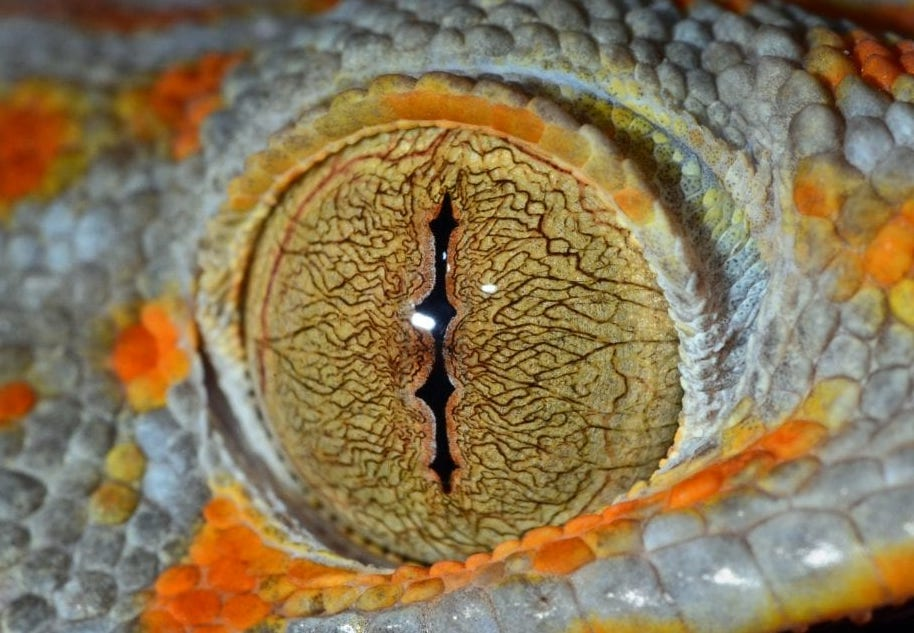
\includegraphics[width=.4\linewidth]{figures/simplesystem/Tokay-Gecko-Eye-1440x954.jpg}} 
}[-4cm]

\subsection{A Catalog of Edges}

Edges denote image regions where there are strong changes of the image  with respect to location. Those variations can be due to a multitude of scene factors (e.g., occlusion boundaries, changes in surface orientation, changes in surface albedo, shadows).

\begin{figure}[t]
\centerline{
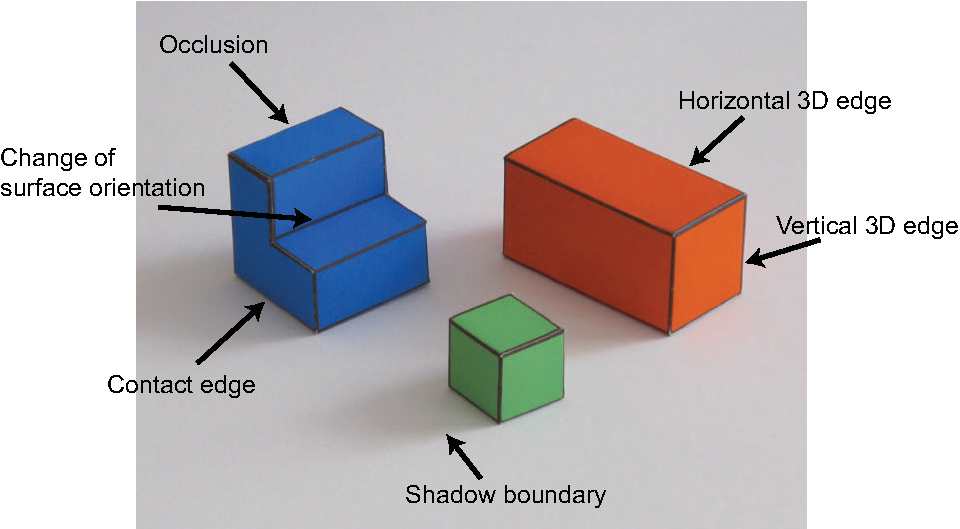
\includegraphics[width=.9\linewidth]{figures/simplesystem/edgeLabeling.pdf}
} 
\caption{Edges denote image regions where there are sharp changes of the image intensities. Those variations can be due to a multitude of scene factors (e.g., occlusion boundaries, changes in surface orientation, changes in surface albedo, and shadows).} 
\label{fig:edgeLabeling}
\end{figure}

One of the tasks that we will solve first is to classify {\bf image edges}\index{Edge!types} according to their most probable cause. We will use the following classification of image boundaries (\fig{\ref{fig:edgeLabeling}}):
\begin{itemize}
\item {\bf Object boundaries}: These indicate pixels that delineate the boundaries of any object. Boundaries between objects generally correspond to changes in surface color, texture, and orientation. 

\item Changes in {\bf surface orientation}: These indicate locations where there are strong image variations due to changes in the surface orientations. A change in surface orientation produces changes in the image intensity because intensity is a function of the angle between the surface and the incident light.  

\item {\bf Shadow edges}: This can be harder than it seems. In this simple world, shadows are soft, creating slow transitions between dark and light.
\end{itemize}

We will also consider two types of object boundaries:
\begin{itemize}
\item {\bf Contact edges}: This is a boundary between two objects that are in physical contact. Therefore, there is no depth discontinuity. 

\item {\bf Occlusion boundaries}: Occlusion boundaries happen when an object is partially in front of another. Occlusion boundaries generally produce depth discontinuities. In this simple world, we will position the objects in such a way that objects do not occlude each other but they will occlude the background.
\end{itemize}

Despite the apparent simplicity of this task, in most natural scenes, this classification is very hard and requires the interpretation of the scene at different levels. In other chapters we will see how to make better edge classifiers (i.e., by propagating information along boundaries, junction analysis, inferring light sources).


\subsection{Extracting Edges from Images}

The first step will consist in detecting candidate edges in the image.
\index{Edge!detection}
%We will describe other techniques in detail in lecture 14. 
Here we will start by making use of some notions from differential geometry. If we think of the image $\img (x,y)$ as a function of two (continuous) variables (\fig{\ref{fig:imageAsSurface}}), we can measure the degree of variation using the gradient:
\begin{eqnarray}
\nabla \img = \left( \frac{\partial \img}{\partial x}, \frac{\partial \img}{\partial y} \right)
\end{eqnarray}
The direction of the gradient indicates the direction in which the variation of intensities is larger. If we are on top of an edge, the direction of larger variation will be in the direction perpendicular to the edge. 

\marginnote{Gradient of an image at one location:
\\~\\
\centerline{\includegraphics[width=.35\linewidth]{figures/simplesystem/gradient2.eps}
} 
}[-0.5in]

However, the image is not a continuous function as we only know the values of the $\img (x,y)$ at discrete locations (pixels). Therefore, we will approximate the partial derivatives by:
\begin{eqnarray}
\frac{\partial \img}{\partial x} & \simeq & \img(x,y) - \img(x-1,y) \\
\frac{\partial \img}{\partial y} & \simeq & \img(x,y) - \img(x,y-1) 
\label{eq:image_partial_derivatives_aprox}
\end{eqnarray}

A better behaved approximation of the partial image derivative can be computed by combining the image pixels around $(x,y)$ with the weights:
\begin{eqnarray}
\frac{1}{4} \times
\left [
\begin{matrix}
-1 & 0 & 1 \\
-2 & 0 & 2 \\
-1 & 0 & 1 
\end{matrix}
\right ] \nonumber
\end{eqnarray}
We will discuss these approximations in detail in \chap{\ref{chapter:image_derivatives}}. 

From the image gradient, we can extract a number of interesting quantities:
\index{Edge!strength} \index{Edge!orientation}
\begin{align}
    e(x,y) &= \lVert \nabla \img(x,y) \rVert   & \quad\quad \triangleleft \quad \texttt{edge strength}\\
    \theta(x,y) &= \angle \nabla \img =  \arctan \left( \frac{\partial \img / \partial y}{\partial \img / \partial x} \right) & \quad\quad \triangleleft \quad \texttt{edge orientation}
\end{align}
\marginnote{The edge strength is the gradient magnitude, and the edge orientation is perpendicular to the gradient direction.}

The unit norm vector perpendicular to an edge is:
\begin{eqnarray}
{\bf n} = \frac{\nabla \img}{\lVert \nabla \img \rVert}
\end{eqnarray}



%\subsection{Edge classification}



The first decision that we will perform is to decide which pixels correspond to edges (regions of the image with sharp intensity variations) and which ones belong to uniform regions (flat surfaces). We will do this by simply thresholding the edge strength $e(x,y)$. 
%In lecture 14 we will discuss more sophisticated edge detectors. 
In the pixels with edges, we can also measure the edge orientation $\theta(x,y)$. \Fig{\ref{fig:gradient}} visualizes the edges and the normal vector on each edge. 


\begin{figure}[t]
\centerline{
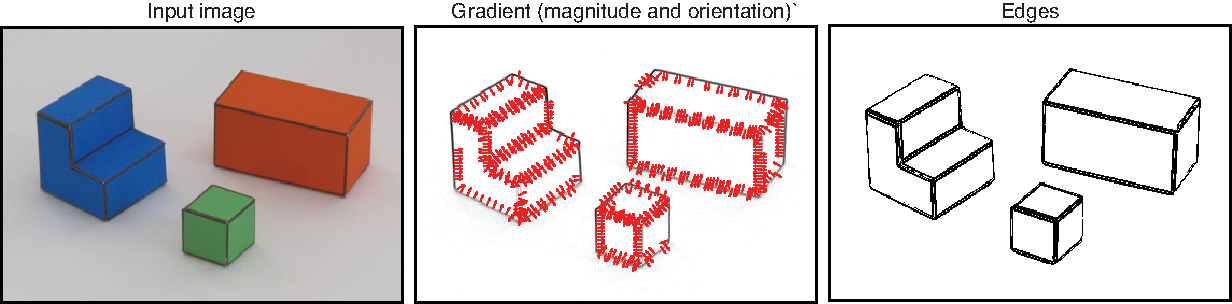
\includegraphics[width=1\linewidth]{figures/simplesystem/gradient.pdf}
} 
\centerline{
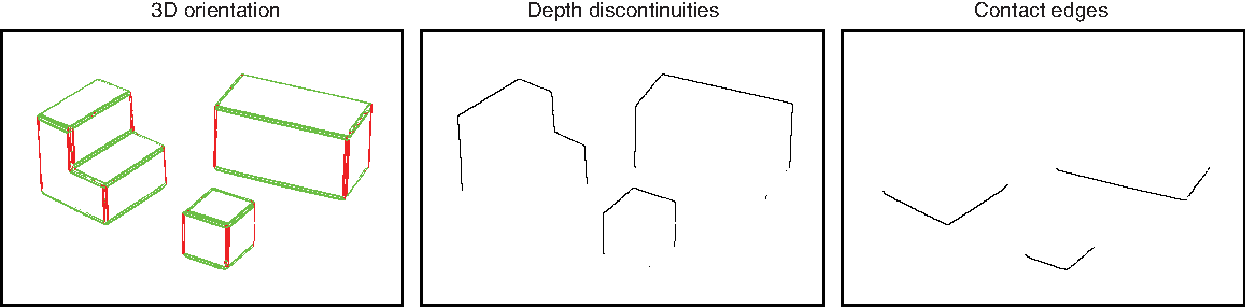
\includegraphics[width=1\linewidth]{figures/simplesystem/edgeTypes.pdf}
} 
\caption{Gradient and edge types.} 
\label{fig:gradient}
\end{figure}

\section{From Edges to Surfaces}

We want to recover world coordinates $X(x,y)$, $Y(x,y)$, and $Z(x,y)$ for each image location $(x,y)$. Given the simple image formation model described before, recovering the $X$ world coordinates is trivial as they are directly observed: for each pixel with image coordinates $(x,y)$, the corresponding world coordinate is $X(x,y) = x$. Recovering $Y$ and $Z$ will be harder as we only observe a mixture of the two world coordinates (one dimension is lost due to the projection from the 3D world into the image plane). Here we have written the world coordinates as functions of image location $(x,y)$ to make explicit that we want to recover the 3D locations of the visible points. 

In this simple world, we will formulate this problem as a set of linear equations. 



\subsection{Figure/Ground Segmentation}



Segmentation of an image into figure and ground is a classical problem in human perception and computer vision that was introduced by {\bf Gestalt psychology}.\index{Gestalt psychology}

\marginnote{The classical visual illusion ``two faces or a vase'' is an example of {\bf figure-ground} segmentation problem.\\[6pt]
\centerline{

\includegraphics[width=.4\linewidth]{figures/simplesystem/figure-ground.eps}
}}

In this simple world deciding when a pixel belongs to one of the {\bf foreground} objects or to the {\bf background} can be decided by simply looking at the color values of each pixel. Bright pixels that have low saturation (similar values of the red-blue-green [RBG] components) correspond to the white ground plane, and the rest of the pixels are likely to belong to the colored blocks that compose our simple world. In general, the problem of {\bf image segmentation} into distinct objects is a very challenging task.% that we will study in lecture 9. 

Once we have classified pixels as ground or figure, if we assume that the background corresponds to a horizontal ground plane, then for all pixels that belong to the ground we can set $Y(x,y)=0$. For pixels that belong to objects we will have to measure additional image properties before we can deduce any geometric scene constraints. 



\subsection{Occlusion Edges}

An occlusion boundary separates two different surfaces at different distances from the observer. 
Along an occlusion edge, it is also important to know which object is in front as this will be the one owning the boundary. Knowing who owns the boundary
 is important as an edge provides cues about the 3D geometry, but those cues only apply to the surface that owns the boundary. 
 \marginnote{{\bf Border ownership}: The foreground object is the one that owns the common edge.\\[6pt]
\centerline{

\includegraphics[width=.4\linewidth]{figures/simplesystem/border_ownership.eps}
}
The dotted lines belong to the object in front.
}

In this simple world, we will assume that objects do not occlude each other (this can be relaxed) and that the only occlusion boundaries are the boundaries between the objects and the ground. However, as we describe subsequently, not all boundaries between the objects and the ground correspond to depth gradients.



\subsection{Contact Edges}

Contact edges are boundaries between two distinct objects but where there exists no depth discontinuity. Despite that there is not a depth discontinuity, there is an occlusion here (as one surface is hidden behind another), and the edge shape is only owned by one of the two surfaces. 

In this simple world, if we assume that all the objects rest on the ground plane, then we can set $Y(x,y)=0$ on the contact edges.
Contact edges can be detected as transitions between the object (above) and ground (below). In our simple world only horizontal edges can be contact edges. We will discuss next how to classify edges according to their 3D orientation.


\begin{figure}
\centerline{
\includegraphics[width=.5\linewidth]{figures/simplesystem/ground_figure_points.eps}
} 
\caption{For each vertical line (shown in red), scanning from top to bottom, transitions from ground to figure are occlusion boundaries, and transitions from figure to ground are contact edges. This heuristic will fails when an object occludes another.} 
\label{fig:ground_figure_points}
\end{figure}

\subsection{Generic View and Nonaccidental Scene Properties}

Despite that in the projection of world coordinates to image coordinates we have lost a great deal of information, there are a number of properties that will remain invariant and can help us in interpreting the image. Here is a list of some of those invariant properties:
\begin{itemize}
\item Collinearity: a straight 3D line will project into a straight line in the image.
\item Cotermination: if two or more 3D lines terminate at the same point, the corresponding projections will also terminate at a common point. 
%\item Intersection: if two 3D lines intersect at a point, the projection will result in two intersecting lines.
%\item Parallelism: (under weak perspective)
%\item Symmetry: (under weak perspective)
\item Smoothness: a smooth 3D curve will project into a smooth 2D curve.
\end{itemize}
\marginnote{
\centerline{\includegraphics[width=.7\linewidth]{figures/simplesystem/invariants2.eps}} 
}
%% [FIGURE: show some 3D lines and 2D projections illustrating accidental alignments]

Note that those invariances refer to the process of going from world coordinates to image coordinates. The opposite might not be true. For instance, a straight line in the image could correspond to a curved line in the 3D world but that happens to be precisely aligned with respect to the viewers point of view to appear as a straight line. Also, two lines that intersect in the image plane could be disjointed in the 3D space. 


However, some of these properties (not all), while not always true, can nonetheless be used to reliably infer something about the 3D world using a single 2D image as input. For instance, if two lines coterminate in the image, then, one can conclude that it is very likely that they also touch each other in 3D. If the 3D lines do not touch each other, then it will require a very specific alignment between the observer and the lines  for them to appear to coterminate in the image. Therefore, one can safely conclude that the lines might also touch in 3D. 

These properties are called {\bf nonaccidental properties}\index{Nonaccidental image properties} \cite{Lowe1985} because they will only be observed in the image if they also exist in the world or by accidental alignments between the observer and scene structures. Under a {\bf generic view}\index{Generic view}, nonaccidental properties will be shared by the image and the 3D world \cite{Freeman94b}. 

Let's see how this idea applies to our simple world. In this simple world all 3D edges are either vertical or horizontal.  Under parallel projection and with the camera having its horizontal axis parallel to the ground, we know that vertical 3D lines will project into vertical 2D lines in the image. Conversely, horizontal lines will, in general, project into oblique lines. Therefore, we can assume than any vertical line in the image is also a vertical line in the world. 

However, the assumption that vertical 2D lines are also 3D vertical lines will not always work. As shown in \fig{\ref{fig:accidentalAlignments}}, in the case of the cube, there is a particular viewpoint that will make an horizontal line project into a vertical line, but this will require an accidental alignment between the cube and the line of sight of the observer. Nevertheless, this is a weak property and accidental alignments such as this one can occur, and a more general algorithm will need to account for that.  But for the purposes of this chapter we will consider images with {\bf generic views} only.

 
\begin{figure}[t]
\centerline{
\includegraphics[width=1\linewidth]{figures/simplesystem/accidentalAlignments.pdf}
} 
\caption{The generic-view assumption breaks down for the central image, where the cube is precisely aligned with the camera axis.  
} 
\label{fig:accidentalAlignments}
\end{figure}


In \fig{\ref{fig:gradient}} we show the edges classified as vertical or horizontal using the edge angle. Anything that deviates from 2D verticality by more than 15 degrees is labeled as 3D horizontal.


We can now translate the inferred 3D edge orientation into linear constraints  on the global 3D structure. We will formulate these constraints in terms of $Y(x,y)$. Once $Y(x,y)$ is recovered we can also recover $Z(x,y)$ from \eqn{\ref{eq:projection}}. 

In a 3D vertical edge, using the projection equations, the derivative of $Y$ along the edge will be
\begin{eqnarray}
\partial Y / \partial y & = & 1/ \cos(\theta)
\label{eqn:derivative_Y_along_edge}
\end{eqnarray}


In a 3D horizontal edge, the coordinate $Y$ will not change. Therefore, the derivative along the edge should be zero:
\begin{eqnarray}
\partial Y / \partial {\bf t} & = & 0 
\label{eqn:derivative_Y_along_edge_hor}
\end{eqnarray}
where the vector $\bf t$ denotes direction tangent to the edge, ${\bf t}=(-n_y, n_x)$. 
\marginnote{\centerline{
\includegraphics[width=.4\linewidth]{figures/simplesystem/tangent.eps}
}}
We can write this derivative as a function of derivatives along the $x$ and $y$ image coordinates:
\begin{eqnarray}
\partial Y / \partial {\bf t} =  \nabla Y \cdot {\bf t} = -n_y \partial Y / \partial x + n_x \partial Y / \partial y
\label{eqn:derivative_Y_along_edge_tan}
\end{eqnarray}

When the edges coincide with occlusion edges, special care should be taken so that these constraints are only applied to the surface that owns the boundary. 

In this chapter, we represent the world coordinates $X(x,y)$, $Y(x,y)$, and $Z(x,y)$ as images where the coordinates $x,y$ correspond to pixel locations. Therefore, it is useful to approximate the partial derivatives in the same way that we approximated the image partial derivatives in equations (\ref{eq:image_partial_derivatives_aprox}). Using this approximation, \eqn{\ref{eqn:derivative_Y_along_edge}} can be written as follows:
\begin{eqnarray}
Y(x,y)-Y(x,y-1) & = & 1/ \cos(\theta)
\end{eqnarray}

Similar relationships can be obtained from equations (\ref{eqn:derivative_Y_along_edge_hor}) and (\ref{eqn:derivative_Y_along_edge_tan}).

\subsection{Constraint Propagation}
\label{sect:constraint}

Most of the image consists of flat regions where we do not have such edge constraints and we thus don't have enough local information to infer the surface orientation. Therefore, we need some criteria in order to propagate information from the  boundaries, where we do have information about the 3D structure, into the interior of flat image regions. This problem is common in many visual domains. 

\marginnote{
As shown on the left image bellow, an image patch without context is not enough to infer its 3D shape. 
The same patch shown in the original image (right):\\[6pt]
\centerline{
\includegraphics[width=.3\linewidth]{figures/simplesystem/cube_propagartion_1.eps}~~~~~~~~
\includegraphics[width=.3\linewidth]{figures/simplesystem/cube_propagartion_2.eps}
}
\\[6pt]
Information about its 3D orientation its propagated from the surrounding edges. 
}


In this case we will assume that the object faces are planar. Thus, flat image regions impose the following constraints on the local 3D structure:
\begin{eqnarray}
\partial^2 Y / \partial x^2 & = & 0  \\
\partial^2 Y / \partial y^2 & = & 0 \\  
\partial^2 Y / \partial y \partial x & = & 0 
\end{eqnarray}
That is, the second order derivative of $Y$ should be zero. As before, we want to approximate the continuous partial derivatives. The approximation to the  second derivative can be obtained by applying twice the first order derivative approximated by equations (\ref{eq:image_partial_derivatives_aprox}). The result is
$\partial^2 Y / \partial x^2 \simeq 2Y(x,y)-Y(x+1,y)-Y(x-1,y)$, and similarly for $\partial^2 X / \partial x^2$.

%$
%\left [
%\begin{matrix}
%-1 & 2 & -1 \\
%\end{matrix}
%\right ]
%$, which corresponds to 

\subsection{A Simple Inference Scheme}

All the different constraints described previously can be written as an overdetermined system of linear equations. Each equation will have the form:
\begin{eqnarray}
\mathbf{a}_i \mathbf{Y} = b_i
\end{eqnarray}
where $\mathbf{Y}$ is a vectorized version of the image $Y$ (i.e., all rows of pixels have been concatenated into a flat vector). Note that there might be many more equations than there are image pixels.

We can translate all the constraints described in the previous sections into this form. For instance, if the index $i$ corresponds to one of the pixels inside one of the planar faces of a foreground object, then there will be three equations. One of the planarity constraint can be written as $\mathbf{a}_i = [0, \dots, 0, -1, 2, -1, 0, \dots, 0]$, $b_i=0$, and analogous equations can be written for the other two.

We can solve the system of equations by minimizing the following cost function:
\begin{eqnarray}
J = \sum_i (\mathbf{a}_i\mathbf{Y} - b_i)^2
\end{eqnarray}
where the sum is over all the constraints. 

If some constraints are more important than others, it is possible to also add a weight $w_i$.
\begin{eqnarray}
J = \sum_i w_i (\mathbf{a}_i \mathbf{Y} - b_i)^2
\end{eqnarray}

Our formulation has resulted on a big system of linear constraints (there are more equations than there are pixels in the image). It is convenient to write the system of equations in matrix form:
\begin{eqnarray}
\mathbf{A} \mathbf{Y}  = \mathbf{b}
\end{eqnarray}
where row $i$ of the matrix ${\bf A}$ contains the constraint coefficients $\mathbf{a}_i$. The system of equations is overdetermined ($\mathbf{A}$ has more rows than columns). We can use the pseudoinverse to compute the solution:
\begin{eqnarray}
\bf Y = (\mathbf{A}^T \mathbf{A})^{-1} \mathbf{A}^T \mathbf{b}
\end{eqnarray}
This problem can be solved efficiently as the matrix $\mathbf{A}$ is very sparse (most of the elements are zero).

\subsection{Results}

\Fig{\ref{fig:worldCoordinates}} shows the resulting world coordinates $X(x,y)$, $Y(x,y)$, $Z(x,y)$ for each pixel. The world coordinates are shown here as images with the gray level coding the value of each coordinate (black corresponds to the value 0). 

\begin{figure}[t]
\centerline{
\includegraphics[width=1\linewidth]{figures/simplesystem/worldCoordinates.pdf}
} 
\caption{The solution to our vision problem for the input image of \fig{\ref{fig:edgeLabeling}}.
%the assumptions and inference scheme described below leads to these estimates of 3D world coordinates at each image location. 
World coordinates $X$, $Y$, and $Z$ are shown as images.} 
\label{fig:worldCoordinates}
\end{figure}

There are a few things to reflect on: 
\begin{itemize}
\item It works. At least it seems to work pretty well. Knowing how well it works will require having some way of evaluating performance. This will be important.
\item But it cannot possibly work all the time. We have made lots of assumptions that will work only in this simple world. The rest of the book will involve upgrading this approach to apply to more general input images.
\end{itemize}

Despite that this approach will not work on general images, many of the general ideas will carry over to more sophisticated solutions (e.g., gather and propagate local evidence).  One thing to think about is if information about 3D orientation is given in the edges, how does that information propagate to the flat areas of the image in order to produce the correct solution in those regions? 


Evaluation of performance is a very important topic. Here, one simple way to visually verify that the solution is correct is to render the objects under new view points. \Fig{\ref{fig:views}} shows the reconstructed 3D scene rendered under different view points to show that the 3D structure has been accurately captured. 

\begin{figure}[!h]
\centerline{
\includegraphics[width=1\linewidth]{figures/simplesystem/views.pdf}
} 
\caption{To show that the algorithm for 3D interpretation gives reasonable results we can re-render the inferred 3D structure from different viewpoints.} 
\label{fig:views}
\end{figure}

\section{Generalization}

One desired property of any vision system is it ability to {\bf generalize} outside of the domain for which it was designed to operate. In the approach presented in this chapter, the domain of images the algorithm is expected to work is defined by the assumptions described in \sect{\ref{sec:algo_simple_world}}. Later in the book, when we describe learning-based approaches, the training dataset will specify the domain. 
\marginnote{{\bf Out of domain generalization} refers to the ability of a system to operate outside the {\bf domain} for which it was designed.}
What happens when assumptions are violated? Or when the images contain configurations that we did not consider while designing the algorithm?



Let's run the algorithm with shapes that do not satisfy the assumptions that we have made for the simple world. \Fig{\ref{fig:out_of_domain}} shows the result when the input image violates several assumptions we made (shadows are not soft and the green cube occludes the red one) and when it has one object on top of the other, a configuration that we did not consider while designing the algorithm. In this case the result happens to be good, but it could have gone wrong.



\begin{figure}[t]
\centerline{
\includegraphics[width=1\linewidth]{figures/simplesystem/out_of_domain_example.eps}
} 
\caption{Reconstruction of an out-of-domain example. The input image violates several assumptions we made (shadows are not soft and the green cube occludes the red one) and it has one object on top of the other, a configuration that we did not consider while designing the algorithm. 
%In this case the result happens to be good, but it could have gone wrong easily.
} 
\label{fig:out_of_domain}
\end{figure}

\Fig{\ref{fig:impossible}} shows the {\em impossible steps} inspired from \cite{Adelson99}. On the left side, this shape looks rectangular and the stripes appear to be painted on the surface. On the right side, the shape looks as though it has steps, with the stripes corresponding to shading due to the surface orientation. In the middle, the shape is ambiguous. 
\Fig{\ref{fig:impossible}} shows the reconstructed 3D scene for this unlikely image. The system has tried to approximate the constraints, but for this shape it is not possible to exactly satisfy all the constraints.  


\begin{figure}[t]
\centerline{
\includegraphics[width=1\linewidth]{figures/simplesystem/steps.pdf}
} 
\caption{Reconstruction of an impossible figure (inspired from \cite{Adelson99}): the reconstruction agrees with our 3D perception.} 
\label{fig:impossible}
\end{figure}


\section{Concluding Remarks}

Despite having a 3D representation of the structure of the scene, the system is still unaware of the fact that the scene is composed of a set of distinct objects. For instance, as the system lacks a representation of which objects are actually present in the scene, we cannot visualize the occluded parts. The system cannot do simple tasks like counting the number of cubes. 

A different approach to the one discussed here is model-based scene interpretation, where we could have a set of predefined models of the objects that can be present in the scene and the system can try to decide if they are present or not in the image, and recover their parameters (i.e., pose, color).

Recognition allows indexing properties that are not directly available in the image. For instance, we can infer the shape of the invisible surfaces. Recognizing each geometric figure also implies extracting the parameters of each figure (i.e., pose, size).

%[NOTE: This section needs to be developed a bit more. Or perhaps removed from here?]

%% FIGURE: see what happens with real images. See that the simple vision problem is not that simple.

%\section{Conclusion}


%\Appendix{Linear filtering}

%Convolution

%Writing a filter in matrix form


%\section{From objects back to the image}

Given a detailed representation of the world, we could render the image back, or at least some aspects of it. We can check that we are understanding things correctly and judge if we can make verifiable predictions, such as what we would see if we looked behind the object. Closing the loop between interpretation and input will be productive at some point.

In this chapter, besides introducing some useful vision concepts, we also made use of mathematical tools from algebra and calculus that you should be familiar with.

%\newcommand{\hwproblem}[2] {\noindent \\ {\bf #1} {\it #2}}

\newcommand{\textbox}[1]{\hfill\rule{0ex}{0.01ex}
 \centerline{\fbox{\parbox{\textwidth}{#1}}}}

\clearpage
{\Large Exercises}

% Administration
\textbox{
We provide a python notebook with the code to be completed. You can
run it locally or in Colab. To use Colab, upload it to Google Drive
and select `open in colab',  which will allow you to complete the
problems without setting up your own environment. Once you have
finished, copy the code sections that  you have completed\ as
screenshots to the report. \\
}
\vspace{0.2cm}


\hwproblem{Problem 1}{Perspective and orthographic projections}

The goal of this first exercise is to take images with different settings of a camera to create pictures with perspective projection and with orthographic projection. Both pictures should cover the same piece of the scene. You can take pictures of real places or objects (e.g. your furniture).% (e.g., the street, a living room, ...) or you can also create your own simple world (e.g., you can print \texttt{simpleWorld.pdf} and create your own scenes. I recommend printing on matte paper).

To create pictures with orthographic projection you can do two things: 1) use the zoom of the camera, 2) crop the central part of a picture. You will have to play with the distance between the camera and the scene, and with the zoom or cropping so that both images look as similar as possible, only differing in the type of projection (similar to figure 2.2).

Submit the two pictures and clearly label parts of the images that reveal their projection types.


\hwproblem{Problem 2}{Orthographic projection equations} 

Recall the parallel projection equations:
\begin{gather}
    x = \alpha  X + x_0\\
    y = \alpha (\cos(\theta)Y - \sin(\theta)Z) +y_{0}
\end{gather}
which relate the coordinates of a point in the 3D world to the image coordinates of an orthogonal camera rotated by $\theta$ over the $X$-axis.

Show that the  equations emerge naturally from a series of transformations
applied to the 3D world coordinates $(X,Y,Z)$, of the form:
\begin{gather}
\left[
  \begin{array}{c}
    x \\
    y
  \end{array}
\right] = \alpha \cdot P \cdot R_x(\theta) \cdot
\left[
  \begin{array}{ccc}
    X \\
    Y \\
    Z
  \end{array}
\right] +
\left[
  \begin{array}{c}
    x_0 \\
    y_0
  \end{array}
\right]
\end{gather}
Where $R_x(\theta)$ is a $3\times 3$ matrix corresponding to a rotation over the $X$ axis, $P$ is a $2 \times 3$ matrix corresponding to the orthogonal projection and $\alpha$ is  a scaling factor to account for the size
of the
camera sensor, which is a single scalar when the pixels are square (assumed in this case).  

Then, find $\alpha$, $x_0$ and $y_0$ when the world point $(0, 0, 0)$ projects onto  $(0, 0)$ \ (which corresponds to the center of the image) and the point $(1, 0, 0)$ projects onto $(3, 0)$.



\hwproblem{Problem 3}{Edge and surface constraints}

In Sect.~\ref{sect:constraint}, we have written down the constraints for $Y(x, y)$. Briefly derive the constraints for $Z(x, y)$ along vertical edges, horizontal edges, and flat surfaces.


\hwproblem{Problem 4}{Complete the code}

Fill in the missing lines in the notebook: \texttt{Ch2.ipynb}, and include them in the report as screenshots. First, find a way to classify edges as vertical or horizontal edges. Next, fill in the rest of the conditions of the constraint matrix. The constraints for when the pixel is on the ground have already been done for you as an example. Put the kernel in \texttt{Aij} and the value you expect in \texttt{b} (the conversion to a linear system is done for you later so you don't need to worry about that part).

You only need to modify the locations marked with a \texttt{TODO} comment.

Please make sure to also include your answers for \texttt{vertical\_edges}, \texttt{horizontal\_edges}, and your formulations for \texttt{Aij} and \texttt{b} for the different constraints in the report.

\hwproblem{Problem 5}{Run the code} 

Select some of the images included with the code and show some new viewpoints for them.

Optional: You can also try with new images taken by you if you decide to create your own simple world.

\hwproblem{Problem 6}{Violating simple world assumptions} (1 point)

Find one example from the four images provided with the problem set (\texttt{img1.jpg}, ..., \texttt{img4.jpg}) when the recovery of 3D information fails. Include the image and the reconstruction in your writeup, and explain why it fails.

\hwproblem{Research problem} {The real world} [optional]

\textit{A research problem is a question for which we do not know the answer. In fact, there might not
even be an answer. This question is optional and could be extended into a larger course project.}

The goal of this problem is to test the 3D reconstruction code with real images. A number of the assumptions we have made will not work when the input is real images of a more complex scene. For instance, the simple strategy of differentiating between foreground and background segmentation will not work with other scenes.

Try taking pictures of real-world scenes and propose modifications to the scheme proposed in this lecture so that you can get some better 3D reconstructions. The goal is not to build a general system, but to be able to handle a few more situations.

 
 % ANTONIO
%\ifx\isEmbedded\undefined
%	% Loading common settings
%	\input{macros/common}
%	% Loading common variable definitions 
%	\input{macros/macros}
%	\begin{document} 
%\else
%\fi
%

%\setcounter{chapter}{2}


\chapter{Looking at Images}
\label{chap:looking_at_images}
%\reviewcomment{Unfinished but readable. Text incomplete and missing references.}

\section{Introduction}

Vision is about solving an amazing problem: Can we build a system capable of perceiving its surrounding world using only the information available in the small number of electromagnetic waves that fall into the observer’s sensor (eye or camera), after accidentally bounding off the objects surrounding the observer? How is it possible to sense the world and its three-dimensional (3D) structure without touching it? It seems quite likely that if humans did not have the sense of vision, we would think that solving this problem is impossible.

The goal of this chapter is to present vision not as an engineering problem that we want to solve, but as a set of scientific questions that we want to answer. We want to understand how it is that our visual system can interpret the world the way it does. We want to explain what components of an image can be used to infer certain properties of the world. We want to know what questions about the world can be answered by just looking at object with the light that reaches our eyes.

In this chapter we will not answer any of those questions, instead, we will use images to motivate a set of questions that vision scientists and computer vision engineers have been studying for many years. The goal of this chapter is to help you ask questions about how do you perceive the world around you.

\section{Looking at Individual Pixels}


Before we build systems that can see, it is good to learn to look at images and to pay attention to individual pixels.
\index{Pixel}
The image in \fig{\ref{fig:pexels-retha-ferguson}} is a tiny image with just $32 \times 32$ pixels.
It is so small that we can actually look at each single pixel and think about how it is that we can make sense of it. For instance, let's look at the pixel in row 21 counting from the top, and column 20 counting from the left. That pixel corresponds to a dark gray pixel, which is near a couple of other pixels with similar intensity, surrounded by a set of white pixels. That pixel seems to be a pen, but how do we know what it is? The pen is barely three pixels long and one pixel wide. How can that provide enough information?

\begin{figure}[h!]
    \centerline{
        %\includegraphics[width=.9\linewidth]{figures/visionscience/pexels-retha-ferguson-3059745_32pixels.jpg}
        \includegraphics[width=.8\linewidth]{figures/visionscience/DALLE_32x32.png}
    }
    \caption{A tiny image with 32 $\times$ 32 color pixels. Despite the very low resolution, we can still recognize most of its content. {\em Source}: Original image created with Dall-E, and downsampled with Photoshop.}
    \label{fig:pexels-retha-ferguson}
\end{figure}
% Finally not used: Photo by Retha Ferguson from Pexels
% Original: https://www.pexels.com/photo/woman-in-front-of-her-computer-3059745/
% https://markallenassets.blob.core.windows.net/communitycare/2020/11/edit.Retha-Ferguson-from-Pexels-woman-in-front-of-her-computer-3059745.png
% we use instead photo generated with Dall-E


\marginnote{
    Same image as in \fig{\ref{fig:pexels-retha-ferguson}} but shown small.
    \\[6pt]
    \centerline{
        \includegraphics[width=.20\linewidth]{figures/visionscience/DALLE_32x32.png}}
    \\[6pt]
    Reducing the size helps better recognizing the objects despite containing the same visual information.
}[-3in]

Recognition of the meaning of that pixel can not come just from the intensity of that pixel or the few pixels nearby. There are way too many possible situations in which different objects in the world could map to a similar set of pixel intensities. Instead, is the whole image and the context of the pen that provides the necessary information to recognize the pen. Taken in isolation, those pixels are impossible to recognize. Here we show, from left to right, the hand, the pen, and the blue mug.


\begin{figure}[h!]
    \centerline{
        \includegraphics[width=.17\linewidth]{figures/visionscience/dalle_hand.png}
        ~
        \includegraphics[width=.34\linewidth]{figures/visionscience/dalle_mug.png}
        ~
        \includegraphics[width=.29\linewidth]{figures/visionscience/dalle_pen.png}
        %~
        %\includegraphics[width=.21\linewidth]{figures/visionscience/plant.png}
    }
    \caption{Small image patches from \fig{\ref{fig:pexels-retha-ferguson}} in isolation. It is difficult to recognize image patches outside their natural context.}
    %\label{fig:image_classification}
\end{figure}

%\centerline{
%\includegraphics[width=.15\linewidth]{figures/visionscience/pexels-retha-ferguson-3059745_32blur.jpg}
%}


\marginnote{What is the minimum number of pixels needed to form a recognizable image? The answer depends on the image. It is possible to create visually recognizable images with very few pixels \cite{torralba_2009}.}


\section{The More You Look, the More You See}
%{\bf The more you look, the more you see.} 
Visual perception cannot be formulated as a simple input-output function over predefined domains. Vision is a dynamical system, even when looking at a static image. The longer you look at an image, the more details you see and the better you understand the scene. Just look at the image shown in \fig{\ref{fig:street_in_paris}} and try to write down everything you see down to the smallest detail.

% Some useful reference: https://www.pnas.org/content/112/12/3618

% http://groups.csail.mit.edu/vision/datasets/ADE20K//ADE20K_2016_07_26/images/training/r/restaurant_patio/ADE_train_00015819.jpg
\begin{figure}[t]
    \centerline{
        \includegraphics[width=.98\linewidth]{figures/visionscience/ADE_train_00015819_messed_small.jpg}
    }
    \caption{A street in Paris. Is everything fine in this picture?}
    \label{fig:street_in_paris}
\end{figure}
% Photo by Antonio Torralba


But this feeling of unlimited and effortless understanding of a picture is also an illusion. Do you truly understand everything you see? For instance, are you sure you can make sense of all the chair legs in \fig{\ref{fig:street_in_paris}}? In fact, this image has been manipulated so that some of legs do not correspond to any chair.

\marginnote{When solving a task, as the {\bf visual cognitive load} increases we are more likely to make judgment mistakes.
    % https://graphics.stanford.edu/papers/visual-cognitive-load/klingner_aural_vs_visual_cognitive_load.pdf
}

As you look around the image, notice that each patch you look at is actually a small photo in its own right. In fact, a big image like this contains thousands of tiny images within it (\fig{\ref{fig:tiny_images}}). A single photo can be \textit{big data}; if you chop up this photo you get a big dataset of tiny images.
A common trick in computer vision is to take a method that was developed for processing a dataset and instead apply it to the set of patches in an image, or vice versa.


\begin{figure}[t]
    \centerline{
        \includegraphics[width=1\linewidth]{figures/visionscience/tiny_images.jpg}
    }
    \caption{Each picture contains lots of images.}
    \label{fig:tiny_images}
\end{figure}


% \begin{center}
%     patch : image :: image : dataset
% \end{center}

\section{The Eye of the Artist}

Learning to paint is a great way of learning to see. You start from a white piece of canvas and a finite set of acrylic paints, and your goal is to paint an object that should look real, with shadows, 3D shape, and reflections. What mixtures of paint and what strokes can accomplish that? Artists learn to see the world not by what it represents, but as why it looks the way it does.

The following sequence (\fig{\ref{fig:agata_painting}}), painted by Agata Lapedriza, shows different steps in the painting process of a strawberry. Layer after layer, the artist replicates the light that will fool your eye into seeing a strawberry instead of acrylic paint. It is interesting to see that the realism does not increase monotonically as the painting progresses. For instance, from step 3 to 4, the right side of the strawberry has lost realism. However, those new strokes will become the shading that will make the strawberry pop out from the canvas.

\begin{figure}
    \centerline{
        ~1\includegraphics[width=.22\linewidth]{figures/visionscience/fresa_1.jpg}
        2\includegraphics[width=.22\linewidth]{figures/visionscience/fresa_2.jpg}
        3\includegraphics[width=.22\linewidth]{figures/visionscience/fresa_3.jpg}
        4\includegraphics[width=.22\linewidth]{figures/visionscience/fresa_4.jpg}
    }
    \centerline{
        ~~5\includegraphics[width=.22\linewidth]{figures/visionscience/fresa_5.jpg}
        6\includegraphics[width=.22\linewidth]{figures/visionscience/fresa_6.jpg}
        7\includegraphics[width=.22\linewidth]{figures/visionscience/fresa_7.jpg}
        8\includegraphics[width=.22\linewidth]{figures/visionscience/fresa_8.jpg} % Photo by Antonio Torralba
    }
    \caption{The following sequence shows different steps in the process of painting a strawberry. {\em Source}: Original images by Agata Lapedriza.}
    \label{fig:agata_painting}
\end{figure}


% \section{Every photo contains thousands of tiny images}
% The image below contains a million pixels, and each is a tiny image.

% \begin{center}
%     patch : image :: image : dataset
% \end{center}

% A common trick in computer vision is to take a method that was developed for processing a \textit{dataset} and instead apply it to the set of patches in an image, or vice versa.


\section{Tree Shadows and Image Formation}

When walking under the shadow of a tree on a bright sunny day when the sun is right above us (\fig{\ref{fig:tree_pinholes}}[left]), we can see how some light rays get through the holes left between leaves, creating spots on the floor (\fig{\ref{fig:tree_pinholes}}[right]).


\begin{figure}[h!]
    \centerline{
        \includegraphics[width=.497\linewidth]{figures/visionscience/IMG_2842_tree_pinholes.jpg} % Photo by Antonio Torralba
        ~~\includegraphics[width=.491\linewidth]{figures/visionscience/IMG_2837_tree_shadow.JPG} % Photo by Antonio Torralba
    }
    \caption{The shadow of this tree on a normal day projects dozens of pictures of the sun on the ground.}
    \label{fig:tree_pinholes}
\end{figure}

But something is a bit odd about the shape of the bright spots projected on the floor. We would expect that the spots of light would have irregular shapes as the openings between leaves will have all kinds of irregular profiles (\fig{\ref{fig:tree_pinholes}}[left]). Instead, as shown in \fig{\ref{fig:tree_pinholes}}(right), the spots appear to be circular and of similar size. This observation already puzzled Aristotle. What could be happening?  As a hint, \fig{\ref{fig:tree_shadow_eclipse}} shows the shadow of leaves during a solar eclipse.


\begin{figure}[h!]
    \centerline{
        \includegraphics[width=.9\linewidth]{figures/visionscience/tree_shadow_eclipse2.jpg} % Photo by Bill Freeman
    }
    \caption{During an eclipse, the shadow of the tree contains many copies of the crescent sun.}
    \label{fig:tree_shadow_eclipse}
\end{figure}


One of the most common situations that we often encounter is the {\bf pinhole cameras} formed by the spacing between the leaves of a tree.
\index{Camera!Pinhole camera}
The tiny
holes between the leaves of a tree create a multitude of pinholes. The pinholes created by the leaves project different
copies of the sun on the floor. When the openings between leaves are small enough, the shape of the projected spot light is dominated by the shape of the sun.
This is something we see often but rarely think about the origin of the spotlights that we
see on the floor.


%\centerline{
%    \includegraphics[width=.6\linewidth]{figures/visionscience/trees.jpg}}


In fact, the leaves of a tree create pinholes that produce images in many other situations. We will talk about pinhole cameras in \chap{\ref{chapter:imaging}}.

\section{Horizontal or Vertical}

Looking at the previous picture of the shadow of the tree, another interesting question comes to mind: How do you know you are looking at a picture of the ground? How do you know the orientation of the camera?

Look at the two drawings in \fig{\ref{fig:vertical_or_horizontal}}. The lines in the drawing on the left correspond to tiles in a floor, the line drawing on the right is the same drawing rotated 90 degrees. Which one seems to be an horizontal surface and which one seems vertical? Why? The differences in the line orientations are subtle and yet it produces a very different perception.

\begin{figure}[t]
    \centerline{
        \includegraphics[width=1\linewidth]{figures/visionscience/vertical_or_horizontal.eps}}
    \caption{Line drawings. The one on the left seems to correspond to an horizontal surface while the one on the right looks like a vertical surface.}
    \label{fig:vertical_or_horizontal}
\end{figure}

In the arrangement in the left, there are two {\bf vanishing points} (the points in which parallel lines intersect) and both are above the drawing, compatible with the horizon line. However, on the drawing on the right, one of the vanishing points is below the figure and gives the impression that the camera is looking at a vertical wall (the camera seems to be higher than the visible part of the wall). The horizon line of the plane (the line that connects both vanishing points) is horizontal in the left drawing and vertical on the right one.

%\section{The geometry of vision}




\section{Motion Blur}

When we are in a moving car and we take a picture from the passenger window, often images will appear blurring, specially when taken at night (\fig{\ref{fig:Paris_from_moving_car}}). Blur is due to the fact that the camera sensor is collecting light during a period of time while the car is moving and the picture that results is the average of several translated copies of the same image. However, note that not all of the objects are equally blurry. Things that are far away might still look sharp while things nearby appear very blurry.

\begin{figure}[h!]
    \centerline{
        \includegraphics[width=1\linewidth]{figures/visionscience/motion_blur.jpg}} % Photo by Antonio Torralba
    \caption{Picture of Paris taken from a moving car.}
    \label{fig:Paris_from_moving_car}
\end{figure}

The amount of blur is related to the car speed, the exposure time, and the distance between the camera and each object in the scene. We will talk more about how camera motion relates to distance in \chap{\ref{chapter:3D_motion_and_its_2D_projection}}.

\section{Accidents Happen}

\marginnote{Principle of continuity.
    In the following drawing, we see one wave and one line:
    \\[6pt]
    \centerline{
        \includegraphics[width=.6\linewidth]{figures/visionscience/principle_continuity_1.eps}}
    \\[6pt]
    Despite this, other
    groupings are also
    possible.
    \\[6pt]
    \centerline{
        \includegraphics[width=.6\linewidth]{figures/visionscience/principle_continuity_2.eps}}
}
We learned about the generic view principle in \chap{\ref{chapter:simplesystem}}, and this idea comes up a lot in computer vision. But it turns out that in most photographs it's easy to find accidents. This is because photos contain so many things, thousands of tiny images, and there are so many coincidences that could occur. \Fig{\ref{fig:visionscience:migrant_mother}} shows a famous photo and we will look for some coincidences in it. The coincidences are of a specific variety: generically, if you see smooth, continuous line segments you assume that they lie on a single object because it's quite a coincidence for two objects to line up just so their contours perfectly align. The gestalt psychologists called this the {\bf principle of continuity}. The insets  for \fig{\ref{fig:visionscience:migrant_mother}} show several locations in the photo ``Migrant Mother'' by Dorothea Lange where exactly this happens. Can you find more?

\begin{figure}[h!]
    \centerline{
        \includegraphics[width=1\linewidth]{figures/visionscience/accidents_migrant_mother.jpg}}
    \caption{Source: Migrant Mother (1936), by Dorothea Lange. On the right are four examples of coincidences that violate the Gestalt principle of continuity. From top-left clockwise: finger boundary aligns with lip contour, cloth aligns with eye, creases align on two different shirts, sleeve boundary is tangent to line on a different shirt.}
    \label{fig:visionscience:migrant_mother}
\end{figure}
% image source: https://en.wikipedia.org/wiki/File:Lange-MigrantMother02.jpg
% license: public domain

You have to be careful about this when developing vision algorithms. If you assume \textit{no} accidents will happen, then you will be in for some trouble. This is one reason why older, rule-based methods failed, because they did not handle exceptions to the rules.




\section{Cues for Support}

When can we tell by looking that one object supports another?  Consider the ball over a surface depicted in \fig{\ref{fig:cues_for_suppport}}.  The drop shadow provides a strong cue that the ball is above the surface in figures \ref{fig:cues_for_suppport}(a) and \ref{fig:cues_for_suppport}(c), while the slack string provides evidence for the ball being on the surface in figures \ref{fig:cues_for_suppport}(b) and \ref{fig:cues_for_suppport}(c).
Only \fig{\ref{fig:cues_for_suppport}}{c} is a doctored photograph.

In which of these figures does the ball appear to be in contact with the ground plane?

\begin{figure}[h!]
    \centerline{
    \sublabel{a}{ \includegraphics[width=0.47\linewidth]{figures/visionscience/ballUp.jpg}
        \sublabel{b}{\includegraphics[width=0.47\linewidth]{figures/visionscience/ballDown.jpg} }
    }
    \centerline{
        \sublabel{c}{\includegraphics[width=0.47\linewidth]{figures/visionscience/ballPuzzle.jpg}}
    }
    \caption{Cues for support. The relative location between an object, and its shadow on the ground is a powerful cue for contact.}
    \label{fig:cues_for_suppport}
\end{figure}
% image source: photos by Bill


\section{Looking at Raindrops}

When it rains you get to see a rare sight. Every raindrop refracts a panorama of the scene around it (\fig{\ref{fig:droplets}}). What you are seeing is not just one photo but hundreds of images of the scene, one in each raindrop, all from slightly different angles. It turns out specially designed cameras have been made that do the same thing, and they are called {\bf light field cameras}.
\index{Camera!Light field cameras}
These cameras use an array of tiny lenses rather than raindrops, but the result is similar: they capture what the scene looks like from hundreds of different viewing angles, and from that density of information they can achieve many interesting tricks, such as triangulating the depth of objects in the scene and synthetically refocusing the image after it has been taken.

\begin{figure}[t]
    \centerline{
        \includegraphics[width=1.0\linewidth]{figures/visionscience/droplets.jpg}}
    \caption{A naturally occurring light field camera. This picture of raindrops on a window contains hundreds of tiny images of the scene, one in each raindrop. The images to the right are individual zoomed in raindrops from the photo on the left.}
    \label{fig:droplets}
\end{figure}
% Photo by Phillip Isola


\section{Plato's Cave}

% \begin{figure}[h]
% \centerline{
%      \includegraphics[width=0.8\linewidth]{figures/visionscience/fading_shadows.jpg}}
%      \caption{Vision is analogous to Plato's Allegory of the Cave.  An image is a crude projection of the underlying physical state.}
%  \end{figure}
% % Photo by Phillip Isola

In the \textit{Allegory of the Cave}, Plato imagined a group of prisoners
chained up in a cave whose only experience of the outside world is through shadows cast on the cave's wall.
When we look at images, we think we are directly seeing reality, but actually the situation is much more like Plato's cave. An image is a crude projection of the underlying physical state. It collapses all the 3D geometry into a flat 2D grid of pixels. From any given viewing angle, most of the scene is occluded. Materials are only depicted in terms of how photons bounce off their surfaces; what's below the surface may be completely omitted. When you look at a picture, think about all the things you cannot see. There's more you don't see than you do. One job of a vision system is to infer everything you can't see given everything you can.

\marginnote{The allegory of the cave has several layers of indirection: the shadows are cast by puppets that are controlled by puppeteers who act out interpretations of the broader reality outside.}

\section{How Do You Know Something Is Wet?}

Our visual system allows us to recognize not just objects, but also material. We can tell if something will feel hot or cold, soft or hard, smooth or rugged. We can also recognize if something is wet or not without touching it, as shown in \fig{\ref{fig:wet_sand}}.



\begin{figure}[t]
    \centerline{
        \includegraphics[width=.8\linewidth]{figures/visionscience/wet_sand_2.jpeg}}
    \caption{Why does wet sand look dark? The answer to this question is interesting, but not as much as the question itself.}
    \label{fig:wet_sand}
\end{figure}
% Photo by Antonio Torralba


Why does sand look darker when it's wet? Does everything wet look darker than when it is dry? How can we tell which parts of the sand are dark because they are wet and which ones are dark because they are under a shadow?


\section{Concluding Remarks}

This chapter was about learning to ask questions about what we see, why things look the way they do, and how do we recognize them. There are so many things that we see every day that we recognize by the way they look, and yet we seldom ask ourselves why they look that way. Why does the sky appear blue? Why does the moon always look the same? Why do hot things become redder?
There are many other sources you can consult that explore why things look the way they do in the world. A beautiful book on this topic is \booktitle{Light and Color in the Outdoors} by Marcel Minnaert \cite{Minnaert1993}, first published in 1937.

After reading this chapter, you will not know how to implement anything new, nor will you have learned new math or new algorithms. The goal of this chapter was to show you some of the questions you should ask about the visual world that you experience every day. The exercise to do now is to go around with your camera and take pictures of interesting visual phenomena.

\marginnote{Your brain is like a detective looking at all the clues that reveal what the world is made of.}
 % ANTONIO, BILL, PHILLIP
%\setcounter{chapter}{35}
\chapter{Computer Vision and Society}
\label{chapter:computer_vision_and_society}


\section{Introduction}

The success of computer vision has led to vision algorithms playing an
ever-larger role in society. Face recognition algorithms unlock
our phones and find our friends and family members in photographs;  cameras identify
swimmers in trouble in swimming pools and assist people in driving
cars.

With such a large role in society, one may expect that computer vision mistakes can
have a large impact and have the potential to cause harm, and
unfortunately this is true.  While self-driving cars may save tens of
thousands of lives each year, mistakes in those algorithms can also
lead to human deaths.  A mistaken computer match with a surveillance
photograph may implicate the wrong person in a crime.  Furthermore,
the performance of computer vision algorithms can vary from person to
person, sometimes as a function of protected attributes of the person, such as gender, race, or age.
These are potential outcomes that
the computer vision community needs to be aware of and to
mitigate.

The field of {\bf Algorithmic Fairness}\index{Algorithmic Fairness} studies the performance and fairness
of algorithms across people, groups, and cultures.  It seeks to
address algorithmic biases, and to develop strategies to ensure that computer vision algorithms don't reflect or create biases against different groups of people or cultures.
Entry points to this literature include a number of text and video sources, including \cite{Kearns2020,Gebru2020,Hamidi2018,Garvie2016,Hutchinson2019,Dwork2012,barocas-hardt-narayanan,Hardt2020}.

We review two topics: fairness and ethics.
In \sect{\ref{sect:fairness}}, we describe some current techniques.  This is just a small sampling of work in this quickly evolving area, selected to intersect well with the material in the rest of this book.  There is more literature and more subtleties than can be covered here. Even if our algorithms and datasets were completely free of bias, there are still many ethical concerns regarding the use of computer vision technology.
In \sect{\ref{sect:ethics}}, we pose ethics questions that we encourage computer vision researchers to think about.


\section{Fairness}
\label{sect:fairness}

Modern computer vision algorithms are trained from data, and thus are
influenced by the statistical make-up of the training data.
Correlations between the expressed gender of
individuals and their depicted activities recorded within a dataset
can perpetuate or even amplify societal gender biases captured in the dataset \cite{Zhao2017,dalessandro2017,Noble2018}.  Gender classification systems in 2018 showed performance that depended on skin tone \cite{Buolamwini2018}.


There is a need for datasets, and the algorithms trained from them, to minimize spurious relations between protected attributes of people, such as skin color, age, gender, and the image labels or recognition outputs, such as occupation or other qualities that should not depend on the protected attributes.
Researchers have begun to develop methods to identify and mitigate such biases in either computer vision databases or algorithms.

\subsection{Facial Analysis}

Facial detection asks whether there is a face in some image region, while facial analysis refers to measuring additional attributes of the face, including pose and identity.  It is important to characterize the performance of facial analysis systems across demographic groups, as certain studies have done \cite{Klare2012}.  A large Face Recognition Vendor Test by the National Institute of Standards and Technology (NIST) \cite{Grother2019}  examined the accuracy of face recognition algorithms for different demographic groups defined by sex, age, and race or country of birth. For one dataset, they found
false positive rates were highest in West and East African and East Asian people, and lowest in Eastern European individuals. For the systems offered by many vendors, this effect was large, with differences of up to a factor of 100 in the recognition false positive rates between different countries of birth. In addition, the more accurate face recognition systems showed less bias and
some developers supplied highly accurate identification algorithms for
which false positive differentials were undetectable.
Certain studies \cite{Grother2019} have stressed the importance of reporting both false negative and false positive rates for each
demographic group at that threshold. Others \cite{Cavazos2021} have provided
a checklist for measuring bias in face recognition algorithms.  It is clearly important to understand the biases of any facial analysis system that is put into use, as these characteristics can vary greatly from system to system.

%% https://arxiv.org/pdf/1904.07325.pdf
%% Characterizing the Variability in Face Recognition Accuracy Relative to Race


\subsection{Dataset Biases}
\index{Dataset bias}

One cause of algorithmic bias can be a bias in the contents of the training dataset.
There are many subtleties in the creation and labeling of computer vision datasets \cite{Ramaswamy2021b}.
Any dataset represents only one slice of the possible images and labels that one could capture from the world \cite{Torralba2011}.
Furthermore, the samples taken may well be influenced by the background of the researchers gathering the dataset.
\Fig{\ref{fig:soap}} shows examples of common objects from four different households across the globe.  From left to right, the photographs are shown in decreasing order of the average household income of the region from which the photo was taken.  The object recognition results for six different commercially available image recognition systems are listed below each photograph, showing that the performance is much better for the images from first-world households \cite{DeVries2019},  possibly due to a better representation of imagery from such households in the training datasets of the image recognition systems.

\begin{figure}[t]
  \centerline{
    \epsfig{file=figures/fairness/soap3.jpg,width=1\linewidth}}
  \caption{Images of household items, and their recognized classes by five object recognition systems \cite{DeVries2019}. The systems tend to perform worse for non-Western countries and for lower-income households, such as those of the right two photographs.}
  \label{fig:soap}
\end{figure}



\subsection{Generative Adversarial Networks to Create Unbiased Datasets and Algorithms}

One way to mitigate a biased dataset is to synthetically produce the images needed to provide the necessary balance or coverage.
Generative adversarial networks (GANs), described in \chap{\ref{chapter:generative_models}}, can operate on a dataset  to generate sets of images similar to those of the dataset, but differing from each other in controlled ways, for example, with changes in the apparent gender, age, or race of depicted people.  Such GANs  have been used to develop debiased datasets and algorithms.

Sattigeri et al. \cite{Sattigeri2019} proposed an algorithm they called Fairness GAN, which included a classifier trained to perform {\em as poorly as possible} on predicting the classification result based on a protected attribute.  For example, the algorithm was designed to predict an attractiveness label while gaining no benefit from knowing the gender or skin tone.  The resulting debiased dataset showed some improvement in fairness metrics.

Another study \cite{Ramaswamy2021}  took an alternative approach to the problem of removing correlations between a protected attribute and a target label.  The authors  used GANs to generate pairs of realistic looking images that were balanced with respect to each protected attribute.  \Fig{\ref{fig:augmentation}} shows an example of this.  If ``wearing hat'' is deemed to be the protected attribute, it is desired to remove its correlation in the data with the attribute, ``wearing glasses.'' If no debiasing steps were taken, the algorithm would learn to associate wearing hats with wearing glasses.  The GAN is used to augment the dataset with paired examples of images of people wearing hats both with and without glasses.
When this augmented dataset is combined with the original dataset, performance in a variety of fairness measures is improved.

Still another approach to dataset fairness, by \cite{Zhao2017},
injects constraints to require that the model predictions follow the
distributions observed within the
training data, assuming that the training data has the desired distribution.
See also \cite{Wang2020} for a  benchmark and comparison of techniques for dataset bias mitigation.

\begin{figure}[t]
  \centerline{
    \epsfig{file=figures/fairness/augmentation.jpg,width=1\linewidth}}
  \caption{In this example ``wears hat'' is deemed to be a protected attribute, but it is correlated with another attribute, which in this example is ``wears glasses'' \cite{Ramaswamy2021}. The GAN-based method generates sets of images where wearing hats is not correlated with wearing glasses.}
  \label{fig:augmentation}
\end{figure}


\subsection{Counterfactuals for Analyzing Algorithmic Biases}

It may be difficult to distinguish whether a given biased result is caused by algorithmic bias or by biases in the testing dataset \cite{Balakrishnan2020}.  One way to disentangle those is through experimentation, that is, modifying variables of a probe image and examining the algorithm's decision.  GAN models, when coupled with human labeling to learn directions in the latent space corresponding to changes in the desired attributes, allow for such experimental intervention. Researchers \cite{Balakrishnan2020} have shown that such counterfactual studies may lead to very different conclusions than observational studies alone, which can be influenced by biased correlations in the testing dataset.  (See also related work in counterfactual reasoning by \cite{Denton2019}.)  \Fig{\ref{fig:transect}} shows several {\bf transects} from \cite{Balakrishnan2020}, paths through the GAN's latent space where only one face variable is modified. The variation in an algorithm's classification results along the images of the transect to provide a clean assessment of any bias related to the variable being modified.

\begin{figure}[h!]
  \centerline{
    \epsfig{file=figures/fairness/transect.jpg,width=1\linewidth}}
  \caption{
    %When combined with human labeling to learn directions in the latent space corresponding to desired variables, a GAN can generate {\bf transects}, sequences of face images where only one variable changes. 
    A GAN creates sequences of faces, called {\bf transects}, where only one attribute changes \cite{Balakrishnan2020}.
    %This is done by using human labeling to learn how to make changes in the desired parts of the images. These sequences are called "transects".
    %Resulting algorithmic performance then directly indicates biases.
  }
  \label{fig:transect}
\end{figure}



\subsection{Privacy and Differential Privacy}

Since progress in computer vision often comes via new datasets, which typically show images and activities of people, issues of privacy are very important in computer vision research.  There are many ways in which people can be harmed by either intentional or unintentional participation in a dataset.  Datasets of medical results, financial transactions, views of public places, all can contain information that must remain private.
Conversely, there is a benefit to society of releasing datasets for researchers to study:  associations can be found that will benefit public health or safety.  Consequently, subjects want researchers to work with anonymized versions of their datasets.  Unfortunately, a number of well-known examples have shown that seemingly cleaned data, when combined with another apparently innocuous dataset, can reveal information that was desired to be private.  For example, in 1997, the medical records of the governor of Massachussetts were identified by matching anonymized medical
data with publicly available voter registration records \cite{Kearns2020,Dwork2014}.
%% (but see \cite{Barth-Jones2012} for nuances to the story).  
The combination of the two datasets allowed seemingly de-identified private data to be re-identified.


A very successful theoretical privacy framework, called differential privacy, addresses these issues.
Following the techniques of differential privacy \cite{Dwork2014}  researchers can guarantee to the participants of a study that they will not be affected by allowing their data to be used in a study or analysis,
no matter what other studies, datasets, or information sources are available.

\marginnote{ {\bf Differential privacy} allows extracting aggregated information about a population from a database without revealing information about any single individual.}

Algorithms can be designed for which it can be shown that the guarantee of differential privacy is met
\cite{Kearns2020,Dwork2014}.  One approach is to inject enough randomness into each recorded observation to guarantee that no individual's data can be reconstructed (with probabilistic guarantees that can be made as stringent as desired, at the cost of data efficiency), while still allowing scientific conclusions to be formed by averaging over the many data samples.
A simple example of this approach, described in \cite{Kearns2020}, is the following procedure to query a set of adults to determine what fraction of them have cheated on their partner.  Each surveyed adult is instructed to flip a coin.  If the coin shows heads, they are instructed to answer the question, ``Have you cheated on your partner?'',  truthfully.  If the coin shows tails, they are asked to answer ``yes'' or ``no'' at random, by flipping the coin again and answering ``yes'' if heads and ``no'' if tails.  The resulting responses for each individual are stored.



If the stored data were hacked, or accidentally leaked, no harm would come to the surveyed individuals even though their data from this sensitive survey had been revealed.  Any ``yes" answer could very plausibly be explained as being a result of the subject having been instructed by the protocol to flip a coin to select the answer.  Yet it is still possible to infer the true percentage of ``yes" answers in the surveyed population from the stored data:  the expected value of the measured percentages will be the true ``yes" and ``no" answers in the population.  The price for this differential privacy is that more data must be collected to obtain the same accuracy guarantees in the estimate of the true population averages.

\marginnote{There are also risks associated with the wrong use of differential privacy \cite{Dwork_Kohli_Mulligan_2019}.}

\section{Ethics}
\label{sect:ethics}

Many ethical issues are outside of the traditional training and education of scientists or
engineers, but ethics are important for vision scientists to think
through and grapple with.  Scientists have a distinguished history of engaging
with ethical and moral issues
\cite{Huxley1932,Orwell1948,Kearns2020,Rogaway2015}.

\subsection{Concerns beyond Algorithmic Bias}

Suppose the research community developed algorithms that could recognize and analyze people or objects equally well, regardless of displayed gender, race, age, culture or other class attributes.  Is the community's work toward fairness completed?  Unfortunately, there are still many issues of concern, as pointed out by many authors and speakers \cite{Gebru2020,Gebru2021,Benjamin2019}.
To list a few of these issues:

\begin{itemize}
  \item Face analysis for job hiring.  Companies have used automated facial analysis methods (analyzing expressions and length of responses) as part of their proprietary algorithms for resume screening, although, at least for some cases, that process has stopped after criticism of the fairness of these methods for screening \cite{Kahn2021}.
  \item Automated identification of faces can be used to compile a list of the participants at a public protest, potentially allowing retribution for attendance
        \cite{Garvie2016,Mozur2019}.
  \item People can show a bias toward believing the output of a machine \cite{Cummings2004}, making it more difficult for a person to correct an algorithm's mistake.

  \item There are concerns whether labeling the gender of a person from their appearance could cause distress or harm to some in the LGBTQ community \cite{Hamidi2018,Bennett2021}.
\end{itemize}

We provide a subsequent list of
questions for thought and discussion.  We encourage computer vision students and
practitioners to engage with these questions, and, of course, to continue to ask their own questions as well.  We need to work both as technologists and as citizens to ensure that computer vision technologies are used responsibly.


\subsection{Some Ethical Issues in Computer Vision}

The following are an (incomplete) set of questions that researchers and engineers may keep in mind:

\begin{itemize}
  \item Would you prefer that a person identify someone from a
        photograph, with the potential biases and assumptions that the
        individual may have, or for an algorithm to do so, based on training
        from a dataset which may include biases of its own? See \cite{Kearns2020,Mullainathan2019} for related discussions.
  \item What privacy safeguards must be in place to accept always-on
        camera and voice recording inside people's homes?  Inside your own home?
  \item Traffic fatalities in the US currently result in the tragedy
        of approximately
        30,000 deaths annually, with most of those fatalities being caused by
        driver error. If every vehicle were self-driving, fatalities caused by human error could fall dramatically, yet there will surely still be fatalities caused by machine errors, albeit far fewer than had been caused by humans.  Is that a tradeoff society should make? What should be our threshold of fatalities caused by machine?
        This moral question is a societal-scale
        version of ``the trolley problem''\index{The trolley problem} \cite{Thomson1985}:  A bystander can choose to divert a trolley from the main track to a side track, saving five people who are on that main track, but killing one person who is on the side track.  Should the bystander actively divert the trolley, intentionally killing the person on the side track, who would otherwise have been spared if no action were taken?  These issues are also present for automobile airbags, which save many lives but sometimes injure a small number of  people \cite{Dalmotas1995}, and in other public health issues.
  \item
        Algorithms will never perform exactly as well among all groups of
        people. Within what tolerance must the performance of human analysis
        algorithms be for an algorithm to be considered fair?  Is algorithmic bias being less than human bias sufficient for deployment?
  \item  Some image datasets have contained offensive material \cite{Birhand2021,Barber2019}. How should we decide which concepts or images can be part of a training set?  Is there any need for algorithms to understand offensive words or concepts?
  \item Could potential categorization tasks of humans in photographs  (e.g., gender identity, skincolor,
        age, height) bring
        harm to individuals, and how?
  \item Should computer vision systems ever be used in warfare? In policing? In
        public surveillance?
  \item What is the role of machines in society?  Regarding decisions of person identification,
        do we want people making decisions, with their own difficult-to-measure biases, or do we want machines involved,  with biases that may be measurable?
  \item Do face recognition algorithms suppress public protests?  Consider a world where any face shown in public is always recorded and identifiable.  (We are almost in that world).  What are the consequences of that for personal safety, speech, assembly, and liberties?
  \item What are the most beneficial uses of computer vision?
  \item Which uses have the most potential for harm, or currently cause the most harm?
  \item Is it ok to use computer vision to monitor workers in order to improve their productivity?  In order to improve workplace safety?  In order to prevent workplace harassment?
  \item What criteria would you use to evaluate the pros and cons of using machines or humans for a given task?
  \item Should datasets represent real-world disparities, or represent the world as we want it to be?  How might these choices amplify existing economic disparities?
  \item When should consent be required (and from whom) before using an image to train a computer vision algorithm?
\end{itemize}

\section{Concluding Remarks}

Computer vision, with its expanding roles in society, can both cause harm as well as bring many benefits.  It is important that every computer vision researcher be aware of the potentials for harm, as well as learn techniques to mitigate against those possibilities.  It is our responsibility to bring this technology into our society with care and understanding.


%\reviewcomment{To be written.}

%% ---------------------------------------------------------------
%% send this chapter to:
%% 
%% michael kearns
%% olga russakovsky
%% pietro
%% antonio and phillip.
%% umass amherst guy, uhm, erik learned-miller.

%% if you feel this is superficial and total bullshit, I'd like to hear that now rather than later


 % BILL before we start, let's think about what we are about to study and its consequences. 

%%%%%%%%%%%%%%%%%%%%%%%%%%%%%%%%%%%%%%%%%%%%%%%%%%%%%%%%%
% 2. Physics
\include{parts/part_image_formation}

%\setcounter{chapter}{3}
\chapter{Imaging}\index{Imaging}
\label{chapter:imaging}


\section{Introduction}

Light sources, like the sun or artificial lights, flood our world with light rays.   These reflect off surfaces, generating a field of light rays heading in
all directions through space.  As the light rays reflect from the surfaces,
they generally change in some attributes, such as their brightness or their color.  It is those changes, after reflection from a surface, that let us interpret what we see. In this chapter, we describe how light interacts with surfaces and how those interactions are recorded with a camera.


\section{Light Interacting with Surfaces}
\label{sec:light_interacting_with_surfaces}
Visible light is electromagnetic radiation, exhibiting wave effects like diffraction.  For many imaging models, however, it is helpful to introduce the abstraction of a {\bf light ray}\index{Light ray}, describing the light radiation heading in a particular direction from a particular location in space (\fig{\ref{fig:lightSpray}}).  A light ray is specified by its position, direction, and intensity as a function of wavelength and polarization.  In this treatment, we ignore diffraction effects.

%\begin{comment}
\begin{figure}
\centerline{
\includegraphics[width=0.7\linewidth]{figures/imaging/brdf.eps}}
\caption{A light ray from the sun strikes a surface and generates outgoing rays of intensity and color depending on the angles of the incoming and outgoing rays relative to the surface orientation.}
\label{fig:lightSpray}
\end{figure}
%\end{comment}

Let an incident light ray be from direction $\mathbf{p}$ and
of power, $\imgin(\lambda)$, as a function of spectral wavelength $\lambda$ (\fig{\ref{fig:lightSpray}}).  The
power of the outgoing light, reflected in the direction, $\mathbf{q}$, is determined by what is called the {\bf bidirectional
reflection distribution function}\index{BRDF} (BRDF), $F$, of the surface. If the
surface normal is $\mathbf{n}$, then  outgoing power is some function, $F$, of the surface normal, the incoming and outgoing ray directions, the wavelength, and the incoming light power:
\begin{equation}
\imgout = F \left( \imgin, \mathbf{n}, \lambda, \mathbf{p}, \mathbf{q} \right)
\label{eq:Lambert}
\end{equation}

\subsection{Lambertian Surfaces}

In general, BRDFs can be quite complicated (see \cite{Matusik2002}), describing both diffuse and specular components of reflection.  Even surfaces with completely diffuse reflections can give complicated reflectance distributions \cite{Oren1994}.  
A useful approximation describing diffuse reflection is the {\bf Lambertian model}\index{BRDF!Lambertian}, with a particularly simple BRDF, which we denote as $F_L$.  The outgoing ray intensity, $\imgout$, is a function only of the surface orientation relative to the incoming and outgoing ray directions, the wavelength, a scalar surface reflectance, and the incoming light power:
\begin{equation}
%I_{\mbox{out}} = F_{L}(I_{\mbox{in}} (\lambda), \mathbf{n}, \mathbf{p})  = a I_{\mbox{in}}(\lambda) \cos(\mathbf{n} \cdot \mathbf{p}),
\imgout = F_{L} \left( \imgin (\lambda), \mathbf{n}, \mathbf{p} \right)  = a \imgin(\lambda) \left( \mathbf{n} \cdot \mathbf{p} \right),
\label{eq:lambert}
\end{equation}
where $a$ is the surface {\bf reflectance}, or {\bf albedo}, $\mathbf{n}$ is the
surface normal vector, and $\mathbf{p}$ points toward the source of the incident
light.  Note that the brightness of the outgoing light ray depends on
the orientation of the surface relative to the incident ray, as well
as the reflectance, $a$, of the surface.  For a Lambertian surface,
the intensity of the reflected light is a function of the direction of
the incoming light ray, but not a function of the outgoing direction
of the ray, $\mathbf{q}$.  

\marginnote{Perfectly Lambertian surfaces are not common. The synthetic material called spectralon is the most perfectly Lambertian material.}

\subsection{Specular Surfaces\index{Specular surfaces}}



A widely used model of surfaces with a specular component of reflection is the {\bf Phong reflection model}\index{BRDF!Phong model} \cite{Phong1975}.  The light reflected from a surface is assumed to have three components that result in the observed reflection:  (1) an ambient component, which is a constant term added to all reflections; (2) a diffuse component, which is the Lambertian reflection of \eqn{\ref{eq:Lambert}}; and (3) a specular reflection component. For a given ray direction, $\mathbf{q}$, from the surface, the Phong specular contribution, $\img_{\mbox{Phong spec}}$, is:
\begin{equation}
\img_{\mbox{Phong spec}} = k_s (\mathbf{r} \cdot \mathbf{q})^\alpha \imgin,
\end{equation}
where $k_s$ is a constant, $\alpha$ is a parameter governing the spread of the specular reflection, and the unit vector $\mathbf{r}$ denotes the direction of maximum specular reflection, given by
\begin{equation}
\mathbf{r} = 2(\mathbf{p} \cdot \mathbf{n}) \mathbf{n} - \mathbf{p}
\end{equation}
\Fig{\ref{fig:rendering}} shows the ambient, Lambertian, and Phong shading components of a sphere under two-source illumination, and a comparison with a real sphere under similar real illumination.


\begin{figure}[t]
\centerline{
\sublabelnp{(a) Lambertian}{\includegraphics[width=0.3\linewidth]{figures/imaging/sphereDiffuse.png}}
\sublabelnp{(b) Phong}{\includegraphics[width=0.3\linewidth]{figures/imaging/spherePhongRoughness0.3.png}}
\sublabelnp{(c) Photograph}{\includegraphics[width=0.3\linewidth]{figures/imaging/photoSphere.jpg}}}
\caption{(a and b) Two different renderings of a sphere.  (c) Note the many extra details required of a photorealistic rendering.}
\label{fig:rendering}
\end{figure}


In general, surface reflection behaves
linearly:  the reflection from the sum of two light sources is the sum of the
reflections from the individual sources. 

To associate the reflected light with surfaces in the world, we need to know which light rays came from which direction in space.  That requires that we form an image, which we discuss next.

% what happens when light hits a surface? basic radiometry
% talk about radiance, penoptic function, lightfields here?


\section{The Pinhole Camera and Image Formation}
\label{sec:pinhole_camera_formation}

Naively, we might wonder when looking at a blank wall, why we don't see an image of the scene facing that wall.  The light reflected from
the wall integrates light from every reflecting surface in the room,
so the reflected intensities are an average of light intensities from
many different directions and many
different sources, as illustrated in \fig{\ref{fig:wallpicture}}{a}.  Mathematically, integrating the equation for
Lambertian reflections (equation [\ref{eq:lambert}]) over all possible
incoming light directions $\mathbf{p}$,  we have 
for the intensity reflecting off a Lambertian surface, $\imgout$:
\begin{equation}
\imgout = \int_{\mathbf{p}}  a \imgin(\mathbf{p}) \cos(\mathbf{n} \cdot \mathbf{p}) \mbox{d} \mathbf{p}
\end{equation}
The intensity, $\imgout$, reflecting off a diffuse wall, thus tells us very little about the incoming light intensity $\imgin(\mathbf{p})$ from any given direction $\mathbf{p}$. To learn about $\imgin(\mathbf{p})$, we need to form an image.
Forming an image involves identifying
which rays came from which directions. The role of a camera is to
organize those rays, to convert the cacophony of light rays going
everywhere to a set of measurements of intensities coming from
different directions in space, and thus from different surfaces in the world.


Perhaps the simplest camera is a {\bf pinhole camera}\index{Camera!Pinhole camera}.  A pinhole camera requires a light-tight enclosure, a small hole
that lets light pass, and a projection surface where one senses or views the illumination intensity as a function of position.
\Fig{\ref{fig:wallpicture}}{b} shows the the geometry of a scene, the
pinhole, and a projection surface (wall).  For any given point on the
projection surface, the light that falls there comes from only from one direction, along the straight line joining the surface position and the pinhole.   This creates an image of what's in the world on the
projection plane.%, Figure~\ref{fig:pinhole}~(b).


\begin{figure}[t]
\centerline{
\includegraphics[width=1\linewidth]{figures/imaging/no_picture_on_a_wall_aina.eps}}
\caption{(a) Why there are no pictures appearing on the walls? (b) The pinhole camera restricts the light rays reaching the wall, producing an image to appear.}
\label{fig:wallpicture}
\end{figure}


\begin{comment}
\begin{figure}
\centerline{
\sublabel{a}{
\includegraphics[width=1\linewidth]{figures/imaging/pinhole7.pdf}}}
\centerline{\sublabel{b}{
\includegraphics[width=0.5\linewidth]{figures/imaging/pinhole3.jpg}}
\sublabel{c}{\includegraphics[width=0.3\linewidth]{figures/imaging/gumby.pdf}}}
\caption{(a) Pinhole camera geometry, showing some light rays passing
  through the pinhole aperture to the projection plane.  (b) Image on the projection plane resulting from
  lighting projecting through a pinhole from  the subject, (c). Fig.~\ref{fig:pinholeSize}~(a) shows the configuration of the object, pinhole, and projection plane.}
\label{fig:pinhole}
\end{figure}
\end{comment}

%% \centerline{
%% \sublabel{a}{\includegraphics[width=0.5\linewidth]{figures/imaging/pinholeScene.pdf}}
%% \sublabel{b}{\includegraphics[width=0.5\linewidth]{figures/imaging/pinholeImage.pdf}} }


Making pinhole cameras is easy and it is a good exercise to gain an intuition of the image projection process. The picture in \fig{\ref{fig:pinhole3}} shows a very simple setup similar to the diagram from \fig{\ref{fig:wallpicture}}{b}. This setup is formed by two pieces of paper, one with a hole on it. With the right illumination conditions you can see an image projected on the white piece of paper in front of the opening. You can use this very simple setup to see the effect of changing the distance between the projection plane and the pinhole.


\begin{figure}[t]
\centerline{
\includegraphics[width=.8\linewidth]{figures/imaging/simple_pinhole.jpg}
}
\caption{A simple setting for creating images on a white piece of paper. In front of the white piece of paper we place another piece of black paper with a hole in the middle. The black paper projects a shadow on the white paper and, in the middle of the shadow, appears a picture of the scene in front of the hole. By making the hole large you will get a brighter, but blurrier image.}
\label{fig:pinhole3}
\end{figure}



\Fig{\ref{fig:pinhole2}} shows how to make a pinhole camera using a paper bag with a hole in it.  One sticks their head inside the bag, which has been padded to be opaque.
We encourage readers to make their own pinhole camera designs. The
needed elements are an aperture to let light through, mechanisms to
block stray light,  a projection screen, and some method to view or
record the image on the projection screen. 


\begin{figure}[t]
\centerline{
\includegraphics[width=1\linewidth]{figures/imaging/pinholeBag.pdf}
}
\centerline{
\includegraphics[width=.7\linewidth]{figures/imaging/pinholeBag2.pdf}
}
\caption{A pinhole camera made from paper bags.
Following steps 1--4, you can turn a paper bag into a light-tight pinhole camera, with the viewer inside.  Newspapers can be added between two layers of paper bags to make a light-tight enclosure. The last picture shows the use of the {\bf paper bag pinhole}
\index{Camera!Paper bag camera}
camera by one of the authors. Walking with this camera is challenging because you only get to see an upside-down version of what is behind you (adult supervision required).}
\label{fig:pinhole2}
\end{figure}


We started the section asking why there are no pictures on regular walls and explaining that, for an image to appear, we need some way of restricting the rays that hit the wall so that each location only gets rays from different directions. 
The pinhole camera is one way of forming a picture. But the reality is that, in most settings, light rays are restricted by accidental surfaces present in the space (other walls, ceiling, floor, obstacles, etc.). For instance, in a room, light rays are entering the room via a window, and therefore some of the rays are blocked. In general, the lower part of a wall will see the top of the world outside the window, while the top part of the wall will see the bottom part of the world outside the window. As a consequence, most walls will appear as having a faint blue tone on the bottom because they reflect the sky, as shown in \fig{\ref{fig:accidental}}{a}.


\begin{figure}[t]
%\centerline{
%\includegraphics[width=1\linewidth]{figures/imaging/buildingPinhole3.pdf}
%}
\centerline{
\sublabel{a}{
\includegraphics[width=.28\linewidth]{figures/imaging/room1.jpg}
}
\sublabel{b}{
\includegraphics[width=.625\linewidth]{figures/imaging/room2.jpg}
}
}
\caption{(a) A wall might contain a picture of the world after all. (b) Turning the room into a pinhole camera by closing most of the window helps to focus the picture that appears in the wall. In this case we can see some buildings that are outside the window.}
\label{fig:accidental}
\end{figure}

\marginnote{The world is full of {\bf accidental cameras}\index{Camera!Accidental camera} that create faint images often ignored by the naive observer.}

\subsection{Image Formation by Perspective Projection}

A pinhole camera projects 3D coordinates in
the world to 2D positions on the projection plane of the camera
through the straight line path of each light ray through the pinhole (\fig{\ref{fig:wallpicture}}).  The simple geometry of the camera lets us identify the projection by inspection. The sketch in \fig{\ref{fig:pinhole_names}} shows a pinhole camera and the relevant terminology. 

\begin{figure}[t]
\centerline{
\includegraphics[width=.7\linewidth]{figures/imaging/pinhole_names2.eps}
}
\caption{Coordinate systems. In computer vision it is common to use the {\bf right-hand rule} for choosing the orientation of the 3D coordinate axes.}
\label{fig:pinhole_names}
\end{figure}



\Fig{\ref{fig:pinholeGeometry}} shows the pinhole camera of \fig{\ref{fig:pinhole_names}} but with the box removed, leaving visible the projection plane. \Fig{\ref{fig:pinholeGeometry}} shows the definition of the three coordinate systems that we will use:
\begin{itemize}
    \item {\bf World coordinates}. Let the origin of a World Cartesian coordinate system be the camera's pinhole.
The coordinates of 3D position of a point, $\mathbf{P}$, in the world will be $\mathbf{P} = (X, Y, Z)$, where the Z axis is perpendicular to the
camera's sensing plane (projection plane).
    \item {\bf Camera coordinates} in the {\bf virtual camera plane}. 
    \index{Virtual camera plane}
    The camera projection plane is behind the pinhole and at a distance $f$ of the origin. Let the coordinates in the camera projection plane, $x$ and $y$, be parallel to the world coordinate axes $X$ and $Y$ but in opposite directions, respectively. For simplicity, it is useful to create a virtual camera plane that is radially symmetrical to the projection plane with respect to the origin and it is placed in front of the camera (\fig{\ref{fig:pinholeGeometry}}[a]). This virtual camera plane will create a projected image without the inversion of the image.  The coordinates in the virtual camera plane will have the same sign as the world coordinates, that is, with the same $x$,$y$ coordinates (i.e., both images are identical apart from a flip).
    \item {\bf Image coordinates}, shown in \fig{\ref{fig:pinholeGeometry}}{b}, are typically measured in pixels. Both the camera coordinate system $(x,y)$ and the image coordinate system $(n,m)$ are related by an affine transform as we will discuss later.
\end{itemize}


\begin{figure}[t]
%\centerline{
%\includegraphics[width=0.7\linewidth]{figures/imaging/pinholeGeomGumby.jpg}}
\centerline{
\includegraphics[width=1\linewidth]{figures/imaging/pinhole_geometry2.eps}
}
\caption{(a) Geometry of the pinhole camera. A 3D point $\mathbf{P}$ projects into the location $\mathbf{p}$ in the projection plane, located at a distance $f$ of the pinhole. The virtual camera plane is a radially symmetric projection of the camera plane. (b) Relation between the camera, $(x,y)$, and the image coordinate system $(n,m)$.}
\label{fig:pinholeGeometry}
\end{figure}


If the distance from the sensing plane to the pinhole is $f$ (see \fig{\ref{fig:pinholeGeometry2}})
then similar triangles
gives us the following relations:
\begin{eqnarray} 
x & = & f \frac{X}{Z} 
\label{eq:perspctiveProj1} \\
y & = & f \frac{Y}{Z} 
\label{eq:perspctiveProj}
\end{eqnarray} 
\marginnote{Thales of Miletus, 624 B.C., introduced the notion of {\bf similar triangles.}  It seems he used this to measure the height of Egypt pyramids, and the distance to boats in the sea.} 

Equations (\ref{eq:perspctiveProj1}) and (\ref{eq:perspctiveProj}) are called the {\bf perspective projection
equations}\index{Perspective projection}.  Under perspective projection, distant objects become
smaller, through the inverse scaling by $Z$.  As we will see, the perspective projection
equations apply not just to pinhole cameras but to most lens-based cameras, and
human vision as well. 



\begin{figure}[t]
\centerline{
%\includegraphics[width=.8\linewidth]{figures/imaging/pinholeGeomGumby.jpg}
\includegraphics[width=.7\linewidth]{figures/imaging/similar_triangles2.eps}
}
\caption{Perspective projection equations derived geometrically. From similar triangles, we have $x/f = X/Z$ and $y/f = Y/Z$. Similar triangles are indicated by the same color.}
\label{fig:pinholeGeometry2}
\end{figure}

Due to the choice of coordinate systems, the coordinates in the virtual camera plane have the $x$ coordinate in the opposite direction than the way we usually do for image coordinates $(m,n)$, where $m$ indexes the pixel column and $n$ the pixel row in an image. This is shown in \fig{\ref{fig:pinholeGeometry}}{b}. The relationship between camera coordinates and image coordinates is
\begin{eqnarray}
n & = & - a x + n_0\\
m & = & a y + m_0
\label{eq:cameratoimagecoordinates}
\end{eqnarray}
where $a$ is a constant, and $(n_0, m_0)$ is the image coordinates of the camera optical axis. Note that this is different than what we introduced a simple projection model in \fig{\ref{fig:projection}} in the framework of the simple vision system in \chap{\ref{chapter:simplesystem}}. In that example, we placed the world coordinate system in front of the camera, and the origin was not the location of the pinhole camera.
\marginnote{Biological systems rarely have eyes that are built as pinhole cameras. One exception is the Nautilus, which has evolved a pinhole eye (without any lens).}[-1.2in]


\subsection{Image Formation by Orthographic Projection}

Perspective projection is not the only feasible projection from 3D
coordinates of a scene
down to the 2D coordinates of the sensor plane.  Different camera geometries can lead to other projections.  One alternative to perspective projection is {\bf orthographic projection}\index{Orthographic projection}. \Fig{\ref{fig:orthographics}} shows the geometric interpretation of orthographic (or parallel) projection. 


\begin{figure}[t]
\centerline{
%\includegraphics[width=.8\linewidth]{figures/imaging/pinholeGeomGumby.jpg}
\includegraphics[width=.9\linewidth]{figures/imaging/orthogonal_projection.eps}
}
\caption{Orthographic projection. Projection is done by parallel rays orthogonal to the projection plane. In this example, we have $x = X$ and $y = Y$.}
\label{fig:orthographics}
\end{figure}

In this projection, as the rays are orthogonal to the projection plane, the size of
objects is independent of the distance to the camera. The projection equations are generally written as follows:
\begin{eqnarray}
x & = & k X \nonumber \\
y & = & k Y
\label{eq:orthographicProj}
\end{eqnarray}
where the constant scaling factor $k$ accounts for change of units and is a fixed global image scaling.

Orthographic projection is a good model for telephoto lenses, where the apparent size of objects in the image
is roughly independent of their distance to the camera.  
We used this projection when building the simple visual system in \chap{\ref{chapter:simplesystem}}.


\marginnote{Orthographic Projection is a correct model when looking at an infinitely far away object that is infinitely zoomed in, as discussed in \chap{\ref{chapter:simplesystem}}.}

The next section provides another example of a camera producing an orthographic projection. 


\subsection{How to Build an Orthographic Camera?}
\index{Camera!Orthographic camera}

Can we build a camera that has an orthographic projection? What we need is some way of restricting the light rays so that only perpendicular rays to the plane illuminate the projection plane.

One such camera is the {\bf soda straw camera}\index{Camera!Soda straw camera}, shown in \fig{\ref{fig:straw}}, which you can easily build. The example shown in (c) used around 500 straws.  



\begin{figure}
\centerline{
\includegraphics[width=1\linewidth]{figures/imaging/straw_camera.eps}
}
\caption{Straw camera example.  (a) View through parallel straws. (b) The subject is  a hand in sunlight.  (c)
The resulting image of the straw camera (using smaller straws than (a)).  The image projection is orthographic.}
\label{fig:straw}
\end{figure}


A set
of parallel straws allow parallel light rays to pass from the scene to
the projection plane, but extinguish rays passing from all other
directions. It works better if the straws are painted black to reduce internal reflections that might capture light rays not parallel to the straws, resulting in a less sharp picture. 


\Fig{\ref{fig:straw}}{c} shows the resulting image when imagining the scene shown in \fig{\ref{fig:straw}}{b}. The straw camera doesn't invert the image as the pinhole camera does and objects do not get smaller as they move away from the camera. The image projection is orthographic, with a unity scale factor; the object sizes on the projection plane are the same as those of the objects in the world.

% http://strawcamera.com/

\marginnote{A larger straw camera has been built by Michael Farrell and Cliff Haynes \cite{straw2017} with an impressive 32,000 drinking straws.}


Another implementation of an orthographic camera is the telecentric lens that combines a pinhole with a lens. 
%\marginnote{Maybe the fly's eye is somewhat similar to the straw camera?}

%\centerline{
%\sublabelnp{(a) View through straws of straw camera}
%{\includegraphics[width=0.25\linewidth]{figures/imaging/strawElements.jpg}}
%\sublabelnp{(b) outside of straw camera}{\includegraphics[width=0.4\linewidth]{figures/imaging/strawSceneFocus.pdf}}
%\sublabelnp{(c) \href{https://groups.csail.mit.edu/vision/cvbook/videos/IMG_2948.MOV}{video of straw camera projection.}}{\includegraphics[width=0.3\linewidth]{figures/imaging/strawImageContrast.pdf}}}

%% INTRODUCE THIS SOMEWHERE ELSE
%% \subsubsection{Homogeneous coordinates}
%% 
%% The projection matrix for coordinate %% values, r = MR.

\section{Concluding Remarks}

Light reflects off surfaces and scatters in many directions.  Pinhole cameras allow only selected rays to pass to a sensing plane, resulting in a perspective projection of the 3D scene onto the sensor.  Other camera configurations can give other image projections, such as orthographic projections.

At this point, it is a good exercise to build your own pinhole camera and experiment with it. Building a pinhole camera helps in acquiring a better intuition about the image formation process. 




%%%%%%%%%%%%%%%%%%%%%%%%%%%%%%%%%%%%%%%%%%%%%%%%%%%%%%%
\chapter{Lenses}
\label{chapter:lenses}


%\section{Lenses}

\section{Introduction}

While pinhole cameras can form good images, they suffer from a serious drawback:  the images are very dim because not much light passes through the small pinhole to the sensing plane of the pinhole camera. As shown in figures \ref{fig:pinholes} and \ref{fig:pinholeSize}, one can try to let in more light by making the pinhole aperture bigger.  But that allows light from many different positions to land on a given position at the sensor plane, resulting in a bright but blurry image.  Putting a lens in the larger aperture can give the best of both worlds,  capturing more light while redirecting the light rays entering the camera so that each sensor plane position maps to just one surface point, creating a focused image on the sensor plane.  Here we analyze how light passes through lenses under the approximation of {\bf geometric optics}\index{Geometric optics}, where we ignore effects like diffraction, due to the wave nature of light.



\begin{figure}[h!]
\centerline{
\includegraphics[width=.9\linewidth]{figures/imaging/apertures_and_lenses.pdf}
}
%\centerline{
%\sublabelnp{(a) Image from small pinhole}{\includegraphics[width=0.7\linewidth]{figures/imaging/toby1.pdf}}}
%\centerline{
%\sublabelnp{(b) Image from large pinhole}{\includegraphics[width=0.7\linewidth]{figures/imaging/toby2.pdf}}}
%\centerline{
%\sublabelnp{(c) Image from lens within the large pinhole}{\includegraphics[width=0.7\linewidth]{figures/imaging/toby3.pdf}}}
\caption{Brightness/sharpness trade-offs in image formation. From left to right a small pinhole will create a sharp image, but lets in little light, so the image may appear dark for a given exposure time. A larger pinhole lets in more light and generates a brighter image, but each sensor element records light from many different image positions, creating a blurry image. A lens can collect light reflected over many different angles from a single point, allowing a bright, sharp image.}
\label{fig:pinholes}
\end{figure}


\begin{figure}
\centerline{
\includegraphics[width=1\linewidth]{figures/imaging/gumbyEdited.jpg}
}
%\centerline{
%\sublabel{a}{\includegraphics[width=0.5\linewidth]{figures/imaging/pinhole3.pdf}}}
%\centerline{
%\sublabel{b}{\includegraphics[width=0.45\linewidth]{figures/imaging/tmpGumbys.pdf}}
%\sublabel{c}{\includegraphics[width=0.4\linewidth]{figures/imaging/pinhole4.pdf}}
%\sublabel{d}{\includegraphics[width=0.3\linewidth]{figures/imaging/gumby.pdf}}}
\caption{Physical demonstration of the trade-offs illustrated in \fig{\ref{fig:pinholes}}. (a) Gumby subject, illumination light,
  barrier with the three apertures, and white projection screen. Also, a light source is added to illuminate the subject. (b) Picture of Gumby. (c)
  Images formed by light through the three apertures. (d) Detail of the three
  apertures (small pinhole, large pinhole, and lens).}
\label{fig:pinholeSize}
\end{figure}




\section{Lensmaker's Formula}
\label{sect:lensmaker}

In general, light changes both its wavelength and its speed as it passes from one material to another.  Those changes at the material interface
will cause the light to bend, an effect called {\bf refraction}\index{Refraction}.  The amount of light bending depends on the change of speed of light within each material, and the orientation of the light ray with respect to the interface surface, according to {\bf Snell's Law}\index{Snell's Law} \cite{Hecht2016}, given in the equation below.  Both the wavelength and the speed of light in a medium are inversely proportional to the {\bf index of refraction}\index{Index of refraction} of that medium, denoted as $n$.  The $n$ for a vacuum is 1.  At a material boundary, for the geometry illustrated in \fig{\ref{fig:snell}}, we have
\begin{equation}
n_1 \sin(\theta_1) = n_2 \sin(\theta_2)
\end{equation}
where $\theta_1$ and  $\theta_2$ are the angles with respect to the surface normal of the incident and outgoing light rays, and $n_1$ and $n_2$ are the  indices of refraction of the materials in region 1 and region 2. Snell's law can be derived by matching the wavelength of light projected along the material interface boundary across each side of the boundary.

\marginnote{Snell's Law relates the bending angles of refraction, $\theta_1$ and $\theta_2$, to the indices of refraction, $n_1$ and $n_2$, at a material interface.}

\begin{figure}
\centerline{
%%\sublabel{a}{\includegraphics[width=0.42\linewidth]{figures/imaging/snell.jpg}}
\sublabel{a}{\includegraphics[width=0.40\linewidth]{figures/imaging/snellcropped.eps}}
\sublabel{b}{\includegraphics[width=0.53\linewidth]{figures/imaging/IMG_2490.JPG}}
}
\caption{(a) Snell's law describes the bending of light at interfaces of differing indices of refraction, $n_1$ and $n_2$, in terms of the angles, $\theta_1$ and $\theta_2$, relative to the interface, or surface, normal. (b) Straw below water surface appears distorted due to refraction at the air/water boundary. Note that (a) and (b) are not trivially connected!}
\label{fig:snell}
\end{figure}


A lens is a specially shaped piece of transparent material, positioned to focus light from a surface point onto a sensor. In an ideal world, a lens focusing light from a surface onto a sensor plane has the property that every light ray from the surface point that passes through the lens is refracted onto a common position at the sensor, no matter what part of the lens the ray from the surface hits.  This dramatically increases the light-gathering ability of the camera system, overcoming the poor light-gathering properties of a pinhole camera system.

To achieve that property, we must find a surface shape that allows for this focusing.
Modern lens surfaces are designed by numerical optimization methods, trading off engineering constraints to achieve the best design, often involving several optical elements and different materials.  But to gain insight into the properties of lenses, we can analytically design a lens surface shape provided we simplify the optical system.

For small angles $\theta$ denoted in radians, $\sin(\theta) \approx \theta$.  If we also assume the index of refraction of air is 1 (it is 1.0003) and denote the index of refraction of lens glass as $n$, then Snell's law, as shown in \fig{\ref{fig:snell}}, becomes
%\marginnote{Snell's law for small angles $\theta_1$ and $\theta_2$.}[.1in]
\begin{equation}
\theta_1 = n \theta_2,    
\end{equation}
for small bending angles $\theta_1$ and $\theta_2$.



Consider a lens, and two points along its optical axis at a distance $a$ and $b$ from the lens, as shown in \fig{\ref{fig:lens}}{a}.
We seek to find a surface shape for a lens which creates the light paths shown in \fig{\ref{fig:lens}}{a}:  light leaving from any direction at point $a$ will be focused to arrive at point $b$.  \Fig{\ref{fig:lens}}{b} shows a view of \fig{\ref{fig:lens}}(a), with angles and distances distorted for clarity of labeling.

\begin{figure}
\centerline{
\sublabel{a}{\includegraphics[width=0.9\linewidth]{figures/imaging/lensRealCropped.pdf}}}
\centerline{
\sublabel{b}{\includegraphics[width=1.0\linewidth]{figures/imaging/lensDistortedCropped.pdf}}}
%% \centerline{
%% \sublabel{c}{\includegraphics[width=0.7\linewidth]{figures/imaging/lensSurface.jpg}}}
\caption{(a) The geometry of a thin lens. (b) Showing the labels of adding angles referenced in table~\ref{tab:lensmaker}, used to describe the conditions for the lens shape, $\theta_S$ to give the desired focusing. Geometry  is distorted for visibility.}
\label{fig:lens}
\end{figure}
% see perspective.key from Bill's laptop dropbox for the keynote source figures


We make use of several approximations that commonly hold for imaging systems: the deviations in angle from the optical axes are very small (i.e., the {\em paraxial approximation}) and the lens is modeled to have negligible thickness compared with other distances along the optical axis (i.e., the {\em thin lens approximation}\index{Lens!thin}).  Under those approximations, we can write simple expressions for the bending angles shown in \fig{\ref{fig:lens}}{b} as a function of $\theta_S$,  the lens surface orientation at height $c$.  Those relations are summarized below in table~\ref{tab:lensmaker}.

The middle row of table~\ref{tab:lensmaker} requires explanation.  The light ray within the lens, depicted in \fig{\ref{fig:lens}}{b}, is not necessarily parallel to the optical axis.  In general, it will be rotated by some angle $\delta$ away from the optical axis, giving $\theta_S = \theta_2 + \delta$, and, at the other lens surface, $\theta_S = \theta_3 - \delta$.  Adding those two equations removes $\delta$ and gives the relation $2 \theta_s = \theta_2 + \theta_3$


\begin{table}
%\marginnote{{\bf Table \ref{tab:lensmaker}}: Relations between angles of thin lens example, \fig{\ref{fig:lens}}{b}} % Hack to get the caption of the table in the margin.
\caption{Relations between angles of thin lens example, \fig{\ref{fig:lens}}{b}}
%\faketablecaption{}
\begin{center}
\begin{tabular}{| c c c c |}
\hline
{\bf Angle}  & {\bf Description} & {\bf Relation} & {\bf Reason} \\
\hline
 $\theta_1 $ &
 Initial angle from optical axis & $\theta_1 = c/a$ & Small angle approx.\\ 
  \hline
  & 
 Angle of refracted ray & & Snell's law, \\ 
  $\theta_2$ & wrt front surface normal & $n \theta_2 = \theta_1 + \theta_S$   & small angle approx. \\ 
 \hline
 &
 Angle of refracted ray & & Symmetry of lens,\\ 
  $\theta_3$ & wrt back surface normal & $2 \theta_S  = \theta_2 + \theta_3$  & thin lens approx.\\ 
 \hline
&
 Angle of ray exiting lens & & Snell's law, \\ 
  $\theta_4 + \theta_S$ & wrt back surface normal & $n \theta_3 = \theta_4+\theta_S$  & small angle approx.\\
 \hline
 $\theta_4$ &
  Final angle from optical axis & $\theta_4 = c/b$ & Small angle approx. \\
  \hline 
\end{tabular}
\end{center}
\label{tab:lensmaker}
\end{table}

If we start from the relation in table~\ref{tab:lensmaker} for $\theta_4$, and substitute for each angle using the relation in each line above, up through $\theta_1 = c/a$, we can algebraically eliminate the angles $\theta_1$ through $\theta_4$ to find the condition on the lens surface angle, $\theta_S$, as a function of the distance $c$ from the optical axis, which  allows for the desired focusing to occur.  The result is as follows: 
\begin{equation}
    \theta_S = \frac{c}{2(n-1)} \left( \frac{1}{a} + \frac{1}{b} \right)
\label{eq:ts1}
\end{equation}
This relationship creates the effect that every ray emanating at a small angle from point $a$ will be focused to point $b$.  \Eqn{\ref{eq:ts1}} shows that the lens surface angle, $\theta_S$, must deviate from flat in linear proportional to the distance $c$ from the center of the lens.

\marginnote{To focus, the lens surface angle, $\theta_S$, must be a {\em linear} function of the distance, $c$, from the center of the lens.}[-.3in]

%\begin{figure}
%\centerline{
%\includegraphics[width=0.3\linewidth]{figures/imaging/sphereLens3.pdf}}
%\caption{Relation between $R$ and $\theta_S$, in \eqn{\ref{eq:ts2}}, for a spherical lens.}
%\label{fig:sphereLens}
%\end{figure}

In the thin lens approximation, both parabolic and spherical shapes satisfy that constraint on the lens surface slope.
For a spherical lens surface, such as \fig{\ref{fig:sphereLens}},  curving according to a radius $R$, we have $\sin(\theta_S) = c/R$.  For small angles $\theta_S$, this reduces to
\begin{equation}
    \theta_S = \frac{c}{R},
    \label{eq:ts2}
\end{equation}
where $R$ is the radius of the sphere, which has the desired property that $\theta_S \propto c$.  


\begin{figure}
\centerline{
\includegraphics[width=0.3\linewidth]{figures/imaging/sphereLens3.pdf}}
\caption{Relation between $R$ and $\theta_S$, in \eqn{\ref{eq:ts2}}, for a spherical lens.}
\label{fig:sphereLens}
\end{figure}

Substituting \eqn{\ref{eq:ts2}} into the focusing condition, 
\eqn{\ref{eq:ts1}} yields the {\bf Lensmaker's Formula}\index{Lensmaker's Formula},
\begin{equation}
\frac{1}{a} + \frac{1}{b} = \frac{1}{f},
\label{eq:lensmaker}
\end{equation}
where the lens {\bf focal length}\index{Focal length}, $f$ is defined to be
\begin{equation}
    f = \frac{R}{2(n-1)}
\end{equation}

It is straightforward to show, by rotating the lens in \fig{\ref{fig:lens}}{a} through an angle $\theta_R$ in the above derivation, thus adding $\theta_R$ to $\theta_S$ in table~\ref{tab:lensmaker},
that the lensmaker's equation also holds for light originating off the optical axis.   Thus, under the paraxial and thin lens approximations, the lens focuses light from points on a plane onto points on a second plane, both perpendicular to the optical axis, as illustrated in \fig{\ref{fig:rotatedLens}}.


\begin{figure}
\centerline{
\includegraphics[width=1\linewidth]{figures/imaging/offAxis.pdf}}
\caption{Considering light from off-axis sources is equivalent to rotating the lens surface by $\theta_R$, for small angles $\theta_R$.  The lens focuses rays from off-axis points like $P_1$, as well as from the on-axis point, $P_0$.}
\label{fig:rotatedLens}
\end{figure}


One can also generalize the equation for the case of a lens with different radii of curvature, $R_1$ and $R_2$ on the front and back faces of the lens.  Defining the left and right surface angles $\theta_{s_1}$ and $\theta_{s_2}$, respectively, the middle row equation of table~\ref{tab:lensmaker} becomes $\theta_{s_1} + \theta_{s_2} = \theta_2 + \theta_3$.  Then, the equation substitutions of Table~\ref{tab:lensmaker}, combined with $\theta_{S_i} = c / R_i$, for $i = 1$ and $2$,
lead to
\begin{equation}
    \frac{1}{f} = (n-1) \left( \frac{1}{R_1} + \frac{1}{R_2} \right)
\end{equation}
Note that some texts (e.g., \cite{Hecht2016}) adopt a sign convention where the back surface of a lens is defined to have negative curvature.


\Fig{\ref{fig:greenLaser}} shows a demonstration of the focusing
property for a thin lens. % of a 20cm focal length.  
The hand, labeled (a), is flicking a laser pointer back and forth,
sending light rays in many directions from a central point during the image exposure, as would a diffuse surface reflection.  All the light rays that strike the lens, labeled (b), are focused to the same green spot, labeled (c), while the light rays passing  outside the lens at (b) reveal their straight line trajectories on the wall at (c).


\begin{figure}
\centerline{
\includegraphics[width=0.6\linewidth]{figures/imaging/greenLaserBrightenedCrop2.jpg}
}
\caption{Demonstration showing that a lens focuses a fan of rays, such as those reflecting from a diffuse surface, to a point.  (a) Here the right hand wiggles a laser pointer back and forth during the photographic exposure, generating a fan of light rays, approximating (in one dimension) rays reflecting from one point on a diffuse surface.   (b) The fan of rays sweeps across a lens, which focuses each ray passing through the lens to the same spot at the wall, (c), regardless of where each ray had entered the lens.  (c) The rays that pass outside the lens form the two line segments on either side.}
\label{fig:greenLaser}
\end{figure}
\clearpage % Avoid using clearpage command 

\section{Imaging with Lenses}
\label{sect:imagingWithLenses}

Armed with the lensmaker's formula and the observation of \fig{\ref{fig:thinLens}}, we can analyze how rays travel through lenses in the approximation of geometrical optics. Light passing through the center of a thin lens, where the front and back surfaces are parallel, proceeds without bending.  Thus a convex thin lens\index{Lens!convex} images as a pinhole camera does, creating a perspective projection.
\begin{figure}
\centerline{
\sublabel{a}{\includegraphics[width=0.25\linewidth]{figures/imaging/centerThick.pdf}}
\sublabel{b}{\includegraphics[width=0.25\linewidth]{figures/imaging/centerThin.pdf}}
\sublabel{c}{\includegraphics[width=0.46\linewidth]{figures/imaging/lenspinhole3.pdf}}
}
\caption{Light travels straight through the center of a thin lens, where front and back surfaces are parallel.  (a) Lens with non-zero thickness.  (b) Idealized thin lens.  (c)  Rays passing through the center of the lens behave like rays passing through a pinhole camera, and thus lenses impose a {\em perspective projection}.}
\label{fig:thinLens}
\end{figure}

Two points on opposite sides of the lens at distances $a$ and $b$ from the lens that satisfy \eqn{\ref{eq:lensmaker}} are known as conjugate points.  Light from one conjugate point, traveling through the lens, focuses to the other conjugate point, and vice versa (see \fig{\ref{fig:lenspropt}}).
The rules for tracing light travel through a lens include the following:
  
\begin{enumerate}
\item Every ray passing through one conjugate point and passing through the lens then passes through the conjugate point.  This is the fundamental focusing property of a lens.
\item Parallel rays entering the lens all focus to a point at distance $f$ behind the lens, per \eqn{\ref{eq:lensmaker}}.  In this case, one of the focal points is at infinity.
\item Any ray passing  through the center of the thin lens proceeds in a straight line, as if through a pinhole at the center of the lens (see \fig{\ref{fig:thinLens}}).  Thus, lenses, like pinholes, render the world in {\em perspective projection}.
\item Because focused rays render positions onto a plane as does a line passing through the center of the lens, then the {\bf magnification} of a lens is simply $a/b$, where $a$ is the distance of an infocus object to the lens, and $b$ is the distance from the lens to a sensor plane.
\end{enumerate}
The above properties allow us to analyze the light paths through simple configurations of lenses.

\begin{figure}
\centerline{
\sublabel{a}{\includegraphics[width=0.15\textwidth]{figures/imaging/lensrays1.pdf}}
\sublabel{b}{\includegraphics[width=0.15\textwidth]{figures/imaging/lensrays2.pdf}}
\sublabel{c}{\includegraphics[width=0.15\textwidth]{figures/imaging/lensrays3.pdf}}
\sublabel{d}{\includegraphics[width=0.15\textwidth]{figures/imaging/lensrays4.pdf}}
\sublabel{e}{\includegraphics[width=0.15\textwidth]{figures/imaging/lensrays5.pdf}}
}
\caption{Showing some conjugate points for a convex thin lens.  }
\label{fig:lenspropt}
\end{figure}
Referring to \fig{\ref{fig:lenspropt}}, the two dots are at distance $f$ from the lens. (a) In \fig{\ref{fig:lenspropt}}{a}, parallel  rays from infinity focus at a distance f from the lens.  \Fig{\ref{fig:lenspropt}}{b–d} show that as a source of light rays moves closer to the lens, they focus further away on the other side, while \fig{\ref{fig:lenspropt}}{e} shows how rays emanating from a distance $f$ from the lens are parallel after the lens, that is, they focus at infinity.

%\clearpage % Avoid using clearpage command 

\subsection{Depth of Field}
%% see these notes:  http://graphics.stanford.edu/courses/cs178-10/applets/dof.html

Assume that the lens is part of a camera, focusing light from the world onto the camera's sensor.  If a plane outside of the camera, called the {\bf focal plane}\index{Focal plane}, and the camera's sensor plane are at conjugate positions, then an object in the focal plane is focussed sharply onto the sensor plane.  All rays from a point on the object's surface will come into focus at a point in the sensor plane.  This will image a point in the focal plane to a {\bf circle of confusion} at the sensor plane, as illustrated in \fig{\ref{fig:circleOfConfusion}}.


\begin{figure}
\centerline{
\includegraphics[width=0.7\linewidth]{figures/imaging/circleOfConfusion.eps}}
\caption{Circle of confusion and depth of field.  Referring to \fig{\ref{fig:rotatedLens}}, if the object of interest and the camera's sensor plane are related as conjugate points, that is, with distances $a$ and $b$ from the camera lens respecting the lensmaker's formula (\eqn{\ref{eq:lensmaker}}), then the object will form an image in sharp focus in the sensor plane. But objects in front of the plane of focus by $\delta_a$ will, in general, come to focus some distance $\delta_b$ behind the sensor plane \cite{Levoy2010}.}
\label{fig:circleOfConfusion}
\end{figure}

Objects closer or further from the focal plane will come into focus behind or in front of the sensor plane, respectively, resulting in a blur circle at the sensor plane, as illustrated in figures~\ref{fig:circleOfConfusion} and \ref{fig:DOFformula}.


\begin{figure}
\centerline{
\includegraphics[width=1\linewidth]{figures/imaging/dof.pdf}}
\caption{Circle of confusion and depth of field.  (Top) Variables used in the computation of the depth of field of a lens.  (Bottom) The elongation of the depth of field size for a given tolerable circle of confusion results from narrowing the lens aperture \cite{Levoy2010}. The catch is that narrowing the aperture results in less light reaching the sensor plane.}
\label{fig:DOFformula}
\end{figure}

The region around the plane of focus that results in a blur at the sensor plane that is smaller than some tolerance is called the {\bf depth of field}\index{Depth of field}.  We can calculate the depth of field from geometric considerations. This derivation follows that of Marc Levoy \cite{Levoy2010}.

A camera's {\bf f-number}\index{f-number}, written $N$, is the ratio of the focal length of the lens divided by the diameter of the lens that light passes through, called the aperture\index{Aperture}, A:  $N = f/A$.  Let the diameter of the circle of confusion be $C$.  If the distance, $U$, of the focal plane to the camera is much larger than the focal length of the lens ($U >> f$)
then the diameter of the focal plane that is imaged onto the circle of confusion is $C$ times the magnification of the imaging system, or approximately $C U/f$, again, for $U >> f$.  Referring to the top of  \fig{\ref{fig:circleOfConfusion}}, by similar triangles, we have 
\begin{equation}
    \frac{D_1 f}{C U} = 
    \frac{U - D_1}{\frac{f}{N}}
\end{equation}
Also by similar triangles, we have
\begin{equation}
    \frac{D_2 f}{C U} =
    \frac{D_2+U}{\frac{f}{N}}
\end{equation}
Defining the depth of field, $D$, to be $D = D_1 + D_2$, and combining terms, we have
\begin{equation}
    D = \frac{2 N C U^2 f^2}{f^4 - N^2 C^2 U^2}
\end{equation}
When the circle of confusion, $C$,  is much smaller than the lens aperture, $f/N$, then the term $N^2 C^2 D^2$ can be ignored relative to $f^4$, and we have
\begin{equation}
    D \approx \frac{2 N C U^2}{f^2}
\end{equation}
Note that for smaller camera f-numbers, $N$ (larger apertures), the depth of field decreases in proportion.  This effect can be seen in the bottom of \fig{\ref{fig:DOFformula}}, and in \fig{\ref{fig:rulers}}.




\begin{figure}
\centerline{
\sublabelnp{(a) f/2.0}{\includegraphics[width=0.3\linewidth]{figures/imaging/f2.0_crop.jpg}}
\sublabelnp{(b) f/4.0}{\includegraphics[width=0.3\linewidth]{figures/imaging/f4.0_crop.jpg}}
\sublabelnp{(c) f/8.0}{\includegraphics[width=0.3\linewidth]{figures/imaging/f8.0_crop.jpg}}
}
\caption{Showing the linear relationship between f-number and depth of field.  From the same camera position, a ruler was photographed, in (a), (b), and (c), using f/2.0, f/4.0, and f/8.0, respectively.  Note the region of sharp focus doubles from (a) to (b), and from (b) to (c).}
\label{fig:rulers}
\end{figure}




\subsection{Concave Lenses}

The lens we designed in \sect{\ref{sect:lensmaker}} was convex.  Also of interest are {\bf concave}\index{Lens!concave} lenses, with the lens surface curve bowing inward toward the center of the lens. For example, consider the concave lens with the surface orientation, $\theta_{Sx} = -\theta_S$ in \eqn{\ref{eq:lensmaker}}.  By the reflection symmetry of the lens surface angles, parallel rays entering a concave lens will be bent away from the lens center by the same amount it would be bent {\em toward} the center axis for a convex lens of the same lens radii of curvature.  This leads to a concave lens bringing parallel rays to a virtual focus, a point from which the diverging rays leaving the lens appear to be emanating.  This is 
illustrated in \fig{\ref{fig:ConcaveLenses}}{b} for on-axis, and \fig{\ref{fig:ConcaveLenses}}{c} for off-axis parallel rays.


\begin{figure}
\centerline{
\sublabel{a}{\includegraphics[width=0.28\linewidth]{figures/imaging/concave1.pdf}}
\sublabel{b}{\includegraphics[width=0.27\linewidth]{figures/imaging/concave2.pdf}}
\sublabel{c}{\includegraphics[width=0.27\linewidth]{figures/imaging/concave3.pdf}}
}
\caption{(a) A convex lens focuses rays to a point.  (b) A concave lens focuses rays to a virtual point.  (c) As with convex lenses, a small shift in the angle of the incoming rays causes a shift in the focus point at the focal plane.}
\label{fig:ConcaveLenses}
\end{figure}


The mathematics of the ray bending is similar to that for convex lenses, except the focal length of concave lenses has a negative value, illustrated in \fig{\ref{fig:ConcaveLenses}}.  The focus point for a set of parallel rays entering a concave lens from the left is also on the {\em left side} of the lens.  It is a {\em virtual focal point}, and from the right side of the lens, the emanating rays appear to be originating from the point at distance $-f$ to the left of the lens.  

\subsection{Lenses in a Telescope}

The properties of convex and concave lenses can be used to make a telescope\index{Telescope},  as Galileo did in the early 1600s \cite{Galileo1610}. We can see how the telescope magnifies the size of objects from geometric considerations. As shown in \fig{\ref{fig:telescope}}{a}, we position a convex lens, lens 1, with a long focal length, $f_1$, and a concave lens, lens 2, with a shorter focal length, $f_2$, such that each are $f_1$ and $f_2$ away from some common point, respectively.  Under those conditions, the configurations of figures \ref{fig:ConcaveLenses}(a) and \ref{fig:ConcaveLenses}(b) will cause parallel rays from a distant object entering lens 1 to become a compressed set of parallel rays leaving lens 2.  Referring to \fig{\ref{fig:telescope}}{b}, an angular deviation of the input rays of $\delta_i$ will become an angular deviation, exiting the convex lens of $\delta_o$.  


\begin{figure}[t]
\centerline{
\sublabel{a}{\includegraphics[width=1\linewidth]{figures/imaging/telescope1.pdf}} }
\centerline{
\sublabel{b}{\includegraphics[width=1\linewidth]{figures/imaging/telescope2.pdf}}
}
\caption{(a) Galilean telescope. The convex lens 1 and the concave lens 2 share the same focal point, marked with a dot, resulting in parallel rays in giving parallel rays out. (b) A small change in the input ray angle gives a larger change in the output ray angle. The magnification of the telescope is the ratio, $M$, of the angular deviation of an output ray, $\delta_o$, to the angular deviation of an input ray, $\delta_i$.  Writing the focal point offset, $d$, in terms of the rays passing through the centers of lenses 1 and 2 gives the relation, $M = f_1/f_2$, where $f_1$ and $f_2$ are the respective ray focal lengths.}
\label{fig:telescope}
\end{figure}

By property 3 of \sect{\ref{sect:imagingWithLenses}}, and the small angle approximation, we have $\delta_i f_1 = d$, because the point $p$ is a distance $f_1$ from lens 1.  Similarly, we have $\delta_o f_2 = d$.  Substituting for $d$ gives
\begin{equation}
M = \frac{\delta_o}{\delta_i} = \frac{f_1}{f_2},
\end{equation}
where we have defined the telescope magnification, $M$, to be the amplification of the parallel ray bending angles.


\Fig{\ref{fig:homemade}} shows a homemade telescope, inspired by Galileo's.  The tube is a 2 in. cardboard mailing tube, with a second tube inserted within it to allow the interlens distance to be adjusted for focusing.  The convex lens at the front of the telescope has a focal length of 50 cm, and the convex lens eyepiece has a focal length of 18 mm, giving a magnification of 27. This is comparable to the 30x magnification of Galileo's telescope. 


\begin{figure}[t]
\centerline{
\sublabel{a}{\includegraphics[width=0.45\linewidth]{figures/imaging/telescope4.jpg}}
\sublabel{b}{\includegraphics[width=0.45\linewidth]{figures/imaging/telescope3.jpg}}
}
\caption{Homemade Galilean telescope. (a) The two lenses of the telescope are mounted in a cardboard mailing tube, with focusing allowed by adjustment of an inserted slightly smaller tube with the eyepiece lens. (b) Mailing tube with the lenses removed from the tube ends.  The rubber bands mount the telescope to a tripod, and tube interior is lined with black paper to reduce stray light.}
\label{fig:homemade}
\end{figure}

\Fig{\ref{fig:moon}} compares images made from this homemade telescope with drawings Galileo made of what he saw through his telescope.  He discovered that our moon had mountains and craters, and was thus not a perfect sphere, as some had thought.  While he could not resolve the rings of Saturn, he could see that there was something different about its shape.  These can all be seen from just two lenses within a tube! 





% \begin{figure}
% \centerline{
% \sublabel{a}% %{\includegraphics[width=0.3\linewidth]{figures/imaging/jupiterJuly23.jpg}}
% \sublabel{b}{\includegraphics[width=0.3\linewidth]{figures/imaging/GalileoJupiterMoons.pdf}}
% }
% \caption{(a) Image of Jupiter photographed at the eyepiece of the Galilean telescope of % Fig.~\ref{fig:telescope}.  Note that several of the four "Medician moons" of Jupiter are visible. The colors are due to lens "chromatic aberrations", and don't reflect image information from the planet. (b) A figure by Galileo \cite{Galileo1610} showing the four moons he discovered and named after his patrons, the Medicis. }
% \label{fig:JupiterMoons}
% \end{figure}

\begin{figure}[t]
\centerline{
%% \sublabel{a}{\includegraphics[width=0.35\linewidth]{figures/imaging/moonJuly24unaided.jpeg}}
%% \sublabel{a}{\includegraphics[width=0.35\linewidth]{figures/imaging/rawMoon6b2022.jpg}}
%% \sublabel{b}{\includegraphics[width=0.35\linewidth]{figures/imaging/moonJuly24x20.jpeg}}
\sublabel{a}{\includegraphics[width=0.45\linewidth]{figures/imaging/moonaug6b2022.jpg}}
\sublabel{b}{\includegraphics[width=0.47\linewidth]{figures/imaging/moonGalileo.jpg}}
}
\caption{(a) Moon as viewed through homemade telescope of Galileo's design, photographed at eyepiece with a cell phone camera.  The telescope magnification is 27x.  (b) Drawing by Galileo of the moon, seen through his telescope, with 30x magnification.}
\label{fig:moon}
\end{figure}

%% include page on lightfield cameras?

\marginnote{With his telescope, Galileo discovered four of the moons of Jupiter.  He called them the Medician Stars, in honor of the brothers of the  Medici family, who were prospective patrons.}

\section{Concluding Remarks}
Pinhole cameras can allow more light to enter the camera aperture only at the expense of image sharpness.  Lenses overcome that tradeoff by focusing all the rays passing through the lens from a point on a surface to a single position on the sensor plane, creating an image that is both sharp and bright.

Using small-angle and thin-lens approximations, we designed a lens surface to have that focusing property, showing that the lens must have a parabolic or spherical shape.

Geometric considerations allow depth-of-field calculations, as well as the design of a simple telescope.


%%%%%%%%%%%%%%%%%%%%%%%%%%%%%%%%%%%%%%%%%%%%%%%%%%%%%%%
%%%%%%%%%%%%%%%%%%%%%%%%%%%%%%%%%%%%%%%%%%%%%%%%%%%%%%%
%%%%%%%%%%%%%%%%%%%%%%%%%%%%%%%%%%%%%%%%%%%%%%%%%%%%%%%

\newcommand{\boldimgworld}{\boldsymbol\ell_{\texttt{w}}}
\newcommand{\boldimgsensor}{\boldsymbol\ell_{\texttt{s}}}
\newcommand{\boldimgground}{\boldsymbol\ell_{\texttt{ground}}}
\newcommand{\imgworld}{\ell_{\texttt{w}}}
\newcommand{\imgsensor}{\ell_{\texttt{s}}}


\chapter{Cameras as Linear Systems}
\label{chapter:cameras_as_linear_systems}


%\section{Cameras as linear systems}

%\reviewcomment{After this point, notation needs to be revised and figures need to be reformatted.}

\section{Introduction}

Lens-based and pinhole cameras are special-case devices where the
light falling on the sensors or the photographic film forms an image.
For other imaging systems, such as medical or astronomical systems, the intensities recorded by the camera may look
nothing like an interpretable image.  Because the optical elements of imaging systems are often linear in their response to light, it is convenient and powerful to describe such general cameras using linear algebra, which then provides a powerful machinery to recover an interpretable image from the recorded data. This formulation also helps to build intuitions about how cameras work and it will allow us think about new types of cameras.


\section{Flatland}

For the simplicity of visualization, let's consider one dimensional (1D)
imaging systems.  As shown in \fig{\ref{fig:flatland_camera_linear}} the sensor is
1D and the scene lives in flatland. 

\begin{figure}
\centerline{
\includegraphics[width=.5\linewidth]{figures/imaging/flatland_camera_linear.eps}
}
\caption{A one dimensional imaging system in flatland. As in \fig{\ref{fig:pinholeGeometry}}, we have reversed the direction of the sensor coordinates.}
\label{fig:flatland_camera_linear}
\end{figure}


Let the light
intensities in the
world be represented by a column vector, $\boldimgworld$.  The value of the $n$-th
component of $\boldimgworld$ gives the intensity of the light at position $n$, heading in the direction of the camera.  There are a few more things to notice in \fig{\ref{fig:flatland_camera_linear}}. The first one is that the axis in the camera sensor is reversed, consistent with \fig{\ref{fig:pinholeGeometry}}. The value $n$ corresponds to image coordinates and the units are pixels. The second is that we are modeling the scene as being a line with varying albedos at a fixed depth from the camera. If the scene had a more complex spatial structure we would have to use the {\bf light field}\index{Light field} in order to use the same linear algebra that we will use in this chapter to model cameras. We will use light fields in \chap{\ref{chapter:nerfs}}.

\marginnote{In this chapter we will approximate the input light by a discrete and finite set of light rays instead of a continuous wave. This approximation allow us to use linear algebra to describe the imaging process.}[-.6in]

\section{Cameras as Linear Systems}


As shown in \fig{\ref{fig:amats1}}{a} the sensor is
1D and the scene lives in flatland.  
Let the sensor
measurements be $\boldimgsensor$ and the unknown scene be $\boldimgworld$.  
If
the camera sensors respond linearly to the light intensity at each
sensor, their measurements, $\boldimgsensor$, will be some linear combination, given by the matrix, $\mathbf{A}$,
of the light intensities:
%\begin{equation}
%\mathbf{y} = \mathbf{A} \mathbf{x}
%\label{eq:likelihood}
%\end{equation}
%\begin{equation}
%\boldimg_{\texttt{sensor}} = \mathbf{A} \boldimg_{\texttt{world}}
%\label{eq:likelihood}
%\end{equation}
\begin{equation}
\boldimgsensor = \mathbf{A} \boldimg_{\texttt{w}}
\label{eq:likelihood}
\end{equation}
We
represent the camera by matrix $\mathbf{A}$.  For the case of a pinhole
camera, and assuming 13 pixel sensor
observations, the camera matrix is just a 13$\times$13 identity matrix, depicted in 
\fig{\ref{fig:amats1}}{b}, as each sensor depends only on the value of a single scene element.  
For the case of conventional lens and pinhole cameras, where the observed intensities,
$\boldimgsensor$, are an image of the reflected intensities in the scene,
$\boldimgworld$, then $\mathbf{A}$ is approximately an identity matrix. For more general cameras, $\mathbf{A}$ may be very different from an
identity matrix, and we will need to estimate $\boldimgworld$ from $\boldimgsensor$.

  In the presence of noise, there may not be a solution
$\boldimgworld$ that exactly satisfies \eqn{\ref{eq:likelihood}}, so we
often seek to satisfy it in a least squares sense.  In most cases, $\mathbf{A}$ is either not invertible, or is poorly
conditioned.  It is often useful
to introduce a regularizer, an additional term in the objective
function to be minimized \cite{Poggio85}.  If the regularization term favors a small
$\boldimg_{\texttt{world}}$, then the objective term to minimize, $E$, could be
%\begin{equation}
%E = |\mathbf{y} - \mathbf{A} \mathbf{x}|^2 + \lambda |\mathbf{x}|^2
%\label{eq:posterior}
%\end{equation}
\begin{equation}
E = \lVert \boldimgsensor - \mathbf{A} \boldimgworld \rVert ^2 + \lambda \lVert \boldimgworld \rVert ^2
\label{eq:posterior}
\end{equation}
The regularization parameter, $\lambda$, determines the trade-off between explaining the observations and satisfying the regularization term. 


\begin{figure}[t]
\centerline{
\includegraphics[width=1\linewidth]{figures/imaging/traditional_pinholes_2.eps}
}
\caption{
(a) Schematic drawing of a small-hole 1D pinhole camera, and (b) the visualization of its imaging matrices $\mathbf{A}$, $\mathbf{A}^{-1}$, and the regularized inverse $\mathbf{B}$.
%:  The imaging matrix relating scene intensities to sensor readings ($\mathbf{A}$); the inverse of that matrix ($\mathbf{A}^{-1}$);  the regularized inverse, ($\mathbf{B}$).  
For the small-pinhole imager, all three matrices are identity matrices.  
(c) Large-hole 1D pinhole camera, and (d) the visualization of its imaging matrices.}
\label{fig:amats1}
\end{figure}

Setting the derivative of \eqn{\ref{eq:posterior}} with respect to the elements of the vector $\boldimgworld$ equal to zero, we have
%\begin{eqnarray}
%0 & = &  \bigtriangledown_x |\mathbf{y} - \mathbf{A} \mathbf{x}|^2 +  \bigtriangledown_x \lambda |\mathbf{x}|^2 \\
%& = &  \mathbf{A}^T \mathbf{A} \mathbf{x} - \mathbf{A}^T \mathbf{y} + \lambda \mathbf{x} \\
%\label{eq:deriv}
%\end{eqnarray}
\begin{eqnarray}
0 & = &  \bigtriangledown_{\boldimgworld} \lVert \boldimgsensor - \mathbf{A} \boldimgworld \rVert ^2 +  \bigtriangledown_{\boldimgworld} \lambda \lVert \boldimgworld \rVert ^2 \\
& = &  \mathbf{A}^T \mathbf{A} \boldimgworld - \mathbf{A}^T \boldimgsensor + \lambda \boldimgworld 
\label{eq:deriv}
\end{eqnarray}
or
\begin{equation}
 \boldimgworld = (\mathbf{A}^T \mathbf{A} + \lambda \mathbf{I})^{-1} \mathbf{A}^T \boldimgsensor 
\label{eq:deriv2}
\end{equation}
Where the matrix $\mathbf{B}=(\mathbf{A}^T \mathbf{A} + \lambda \mathbf{I})^{-1} \mathbf{A}^T$ is the regularized inverse of the imaging matrix $\mathbf{A}$.


%For the simplicity of visualization, let's consider one dimensional (1D) imaging systems.  

%As shown in \fig{\ref{fig:amats1}}{a} the sensor is
1D and the scene lives in flatland.  
Let the sensor
measurements be $\boldimgsensor$ and the unknown scene be $\boldimgworld$.  We
represent the camera by matrix $\mathbf{A}$.  For the case of a pinhole
camera, and assuming 13 pixel sensor
observations, the camera matrix is just a 13$\times$13 identity matrix, depicted in 
\fig{\ref{fig:amats1}}{b}, as each sensor depends only on the value of a single scene element.  


%\begin{figure}
%\centerline{
%\sublabel{a}{\includegraphics[width=0.45\linewidth]{figures/imaging/ph2.pdf}}
%\sublabel{b}{\includegraphics[width=0.45\linewidth]{figures/imaging/amat32.pdf}}}
%\caption{
%(a) Large-hole 1-d pinhole camera. (b) Visualization of imaging matrices:  The imaging matrix relating scene intensities to sensor readings; the inverse of that matrix;  the regularized inverse.  }
%\label{fig:amats2}
%\end{figure}

Next, consider the case of a wide aperture pinhole camera, shown in
\fig{\ref{fig:amats1}}{c}.  If a single pixel in the sensor plane covers exactly two positions of the scene intensities, then the geometry is as shown in \fig{\ref{fig:amats1}}{c}. \Fig{\ref{fig:amats1}}{d} also shows the imaging matrix, $\mathbf{A}$,  its inverse, $\mathbf{A}^{-1}$, and the regularized inverse of the imaging matrix, which will usually give image reconstructions with fewer artifacts as it is less sensitive to noise. Note that $\mathbf{A}^{-1}$ contains lots of fast changes that will make the result very sensitive to noise in the observation. The regularized matrix, $\mathbf{B}$, shown in the bottom row of \fig{\ref{fig:amats1}}{d}, is better behaved.

The following plot (\fig{\ref{fig:2pixelwidepinhole}}) shows an example of an input 1D signal, $\boldimgworld$, and the output of the 2-pixel wide pinhole camera, $\boldimgsensor$. 


\begin{figure}[h]
\centerline{
%\begin{center}
$\begin{array}{cc}
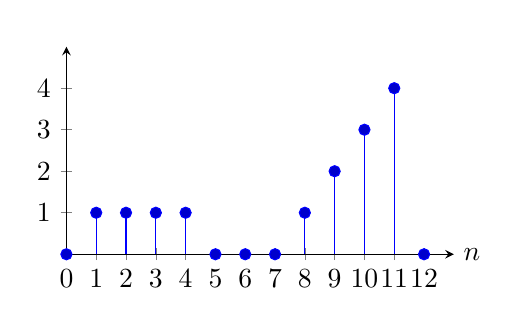
\begin{tikzpicture}
\begin{axis} [width=185pt,height=120pt,
	axis x line=bottom, 
	axis y line=middle, 
	tick align=center,
	every axis x label/.style={at={(current axis.right of origin)},anchor=west},
	every axis y label/.style={at={(current axis.above origin)}, anchor=north east,above=0mm},
	xmin=0, xmax=13,
	xtick={0,...,12},
	xlabel=$n$,
	ymin=0, ymax=5,
	ytick={0,...,4},
	ylabel={$\boldimgworld$}]
\addplot+[ycomb] 
coordinates {(0,0) (1,1) (2,1) (3,1) (4,1) (5,0) (6,0) (7,0) (8,1) (9,2)  (10,3)  (11,4)  (12,0)};
\end{axis}
\end{tikzpicture}
&~
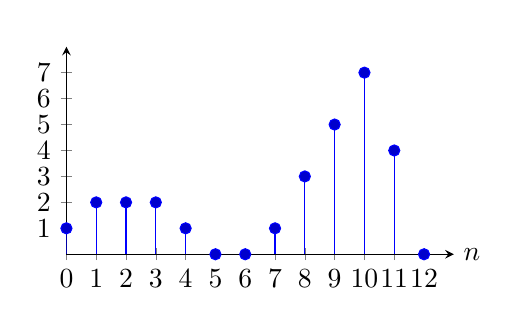
\begin{tikzpicture}
\begin{axis} [width=185pt,height=120pt,
	axis x line=bottom, 
	axis y line=middle, 
	tick align=center,
	every axis x label/.style={at={(current axis.right of origin)},anchor=west},
	every axis y label/.style={at={(current axis.above origin)}, anchor=north east,above=0mm},
	xmin=0, xmax=13,
	xtick={0,...,12},
	xlabel=$n$,
	ymin=0, ymax=8,
	ytick={0,...,7},
	ylabel={$\boldimgsensor$}]
\addplot+[ycomb] 
coordinates {(0,1) (1,2) (2,2) (3,2) (4,1) (5,0) (6,0) (7,1) (8,3) (9,5)  (10,7)  (11,4)  (12,0)};
\end{axis} 
\end{tikzpicture}
\end{array}
$
%\end{center}
}
\caption{Pinhole camera. (left) Input 1D signal, $\boldimgworld$. (right) The output of the two-pixel wide pinhole camera, $\boldimgsensor$.} 
\label{fig:2pixelwidepinhole}
\end{figure}

The output is obtained by multiplying the input vector by the matrix $\mathbf{A}$ shown in \fig{\ref{fig:amats1}}{d}. Each output value is the results of adding up two consecutive input values. The output is nearly identical to the input signal but with a larger magnitude and a bit smoother.

\section{More General Imagers}

Many different optical systems can form cameras and the linear analysis described before can be used to characterize the imaging process.  Even a simple edge will do.  \Fig{\ref{fig:amats3}} shows two non traditional imaging systems that we will analyze in this section. 


\begin{figure}[t]
\centerline{
\includegraphics[width=1\linewidth]{figures/imaging/nontraditional_pinholes_2.eps}
}
\caption{(a) Schematic drawing of an edge camera, and (b) its imaging matrices. (c) A pinspeck camera (an occluder that blocks two of the values on the scene), and (d) its imaging matrices.}
\label{fig:amats3}
\end{figure}

\subsection{Edge Camera}


Consider the example of \fig{\ref{fig:amats3}}{a}. This camera corresponds to an {\bf edge camera}\index{Camera!Edge camera}. This is not a traditional pinhole camera; instead light is blocked only on one side.  




For this camera, the imaging matrix and its inverse are as follows:
%\begin{equation}
%\mathbf{A} = 
%\left( 
%\begin{array}{ccccccccccccc}
%1 & 1 & 1 & 1 & 1 & 1 & 1 & 1 & 1 & 1 & 1 & 1 & 1 \\
%0 & 1 & 1 & 1 & 1 & 1 & 1 & 1 & 1 & 1 & 1 & 1 & 1 \\
%0 & 0 & 1 & 1 & 1 & 1 & 1 & 1 & 1 & 1 & 1 & 1 & 1 \\
%0 & 0 & 0 & 1 & 1 & 1 & 1 & 1 & 1 & 1 & 1 & 1 & 1 \\
%0 & 0 & 0 & 0 & 1 & 1 & 1 & 1 & 1 & 1 & 1 & 1 & 1 \\
%0 & 0 & 0 & 0 & 0 & 1 & 1 & 1 & 1 & 1 & 1 & 1 & 1 \\
%0 & 0 & 0 & 0 & 0 & 0 & 1 & 1 & 1 & 1 & 1 & 1 & 1 \\
%0 & 0 & 0 & 0 & 0 & 0 & 0 & 1 & 1 & 1 & 1 & 1 & 1 \\
%0 & 0 & 0 & 0 & 0 & 0 & 0 & 0 & 1 & 1 & 1 & 1 & 1 \\
%0 & 0 & 0 & 0 & 0 & 0 & 0 & 0 & 0 & 1 & 1 & 1 & 1 \\
%0 & 0 & 0 & 0 & 0 & 0 & 0 & 0 & 0 & 0 & 1 & 1 & 1 \\
%0 & 0 & 0 & 0 & 0 & 0 & 0 & 0 & 0 & 0 & 0 & 1 & 1 \\
%0 & 0 & 0 & 0 & 0 & 0 & 0 & 0 & 0 & 0 & 0 & 0 & 1 
%\end{array}
%\right) .
%\label{eq:edge}
%\end{equation}

\begin{equation}
\mathbf{A} = 
\left[ 
\begin{array}{cccccc}
1 & 1 & 1 & 1 & \dots & 1 \\
0 & 1 & 1 & 1 & ~ & 1 \\
0 & 0 & 1 & 1 & ~ & 1 \\
0 & 0 & 0 & 1 & ~ & 1 \\
\vdots & ~ & ~ & ~ & \ddots & ~ \\
0 & 0 & 0 & 0 & ~ & 1 
\end{array}
\right], 
\mathbf{A}^{-1} = 
\left[ 
\begin{array}{cccccc}
1 & -1 & 0 & 0 & \dots & 0 \\
0 & 1 & -1 & 0 & ~ & 0 \\
0 & 0 & 1 & -1 & ~ & 0 \\
0 & 0 & 0 & 1 & ~ & 0 \\
\vdots & ~ & ~ & ~ & \ddots & ~  \\
0 & 0 & 0 & 0 & ~ & 1 
\end{array}
\right]
\label{eq:edge}
\end{equation}

If we consider the same input as in the pinhole camera example in the previous section, the output signal for the corner camera will look like (\fig{\ref{fig:1dcornercamera}}):

\begin{figure}[h]
\centerline{
%\begin{center}
$
\begin{array}{cc}
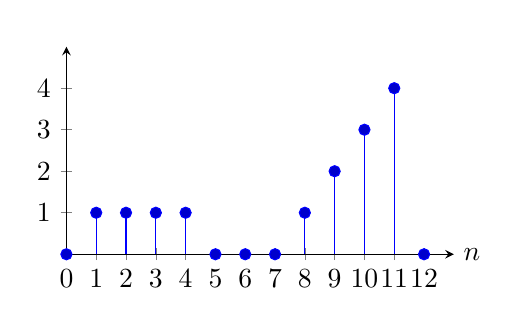
\begin{tikzpicture}
\begin{axis} [width=185pt,height=120pt,
	axis x line=bottom, 
	axis y line=middle, 
	tick align=center,
	every axis x label/.style={at={(current axis.right of origin)},anchor=west},
	every axis y label/.style={at={(current axis.above origin)}, anchor=north east,above=0mm},
	xmin=0, xmax=13,
	xtick={0,...,12},
	xlabel=$n$,
	ymin=0, ymax=5,
	ytick={0,...,4},
	ylabel={$\boldimgworld$}]
\addplot+[ycomb] 
coordinates {(0,0) (1,1) (2,1) (3,1) (4,1) (5,0) (6,0) (7,0) (8,1) (9,2)  (10,3)  (11,4)  (12,0)};
\end{axis}
\end{tikzpicture}
&~
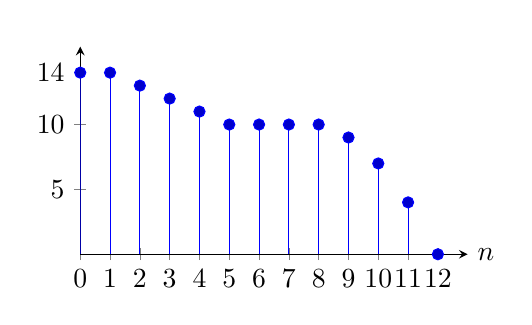
\begin{tikzpicture}
\begin{axis} [width=185pt,height=120pt,
	axis x line=bottom, 
	axis y line=middle, 
	tick align=center,
	every axis x label/.style={at={(current axis.right of origin)},anchor=west},
	every axis y label/.style={at={(current axis.above origin)}, anchor=north east,above=0mm},
	xmin=0, xmax=13,
	xtick={0,...,12},
	xlabel=$n$,
	ymin=0, ymax=16,
	ytick={0,5,10,14},
	ylabel={$\boldimgsensor$}]
\addplot+[ycomb] 
coordinates {(0,14) (1,14) (2,13) (3,12) (4,11) (5,10) (6,10) (7,10) (8,10) (9,9)  (10,7)  (11,4)  (12,0)};
\end{axis} 
\end{tikzpicture}
\end{array}
$
%\end{center}
}
\caption{Edge camera. (left) Input 1D signal, $\boldimgworld$. (right) The output of an edge camera, $\boldimgsensor$.} 
\label{fig:1dcornercamera}
\end{figure}

The output now looks very different than that of a pinhole camera. In the pinhole camera, the output is very similar to the input. This is not the case here where the output looks like the integral of the input (reversed along the horizontal axis). Note that the first value of $\boldimgsensor$ is equal to the sum of all the values of $\boldimgworld$:
\begin{equation}
\imgsensor \left[0 \right] = \sum_{n=0}^{12} \imgworld \left[n \right]
\end{equation}

\Fig{\ref{fig:amats3}}{b} illustrates the imaging matrix, $\mathbf{A}$, and reconstruction matrices for the imager of \eqn{\ref{eq:edge}}. You can think of this imager as computing an integral of the input signal. Therefore, its inverse looks like a derivative. The regularized inverse looks like a blurred derivative (we will talk more about blurred derivatives in \chap{\ref{chapter:image_derivatives}}).
%, as well as for an edge imager where the responses are blurred across several sensor elements.


\subsection{Pinspeck Camera}

\Fig{\ref{fig:amats3}}{c} shows another nontraditional imager. Now, instead of a pinhole we have an occluder. The occluder blocks part of the light (complementary to the large-hole pinhole camera shown in \fig{\ref{fig:amats1}}{c}). What the camera sensor records is the shadow of the occluder.
\marginnote{The shadow of an object is related to the negative of a picture taken of the environment around the object.}
We can write the imaging matrix $\mathbf{A}$, which corresponds to 1-$\mathbf{A}_{pinhole}$ as shown in \fig{\ref{fig:amats1}}{d}. \Fig{\ref{fig:amats3}}{d} also shows its inverse and the regularized inverse. This camera is called a {\bf pinspeck camera}\index{Camera!Pinspeck camera} \cite{CohenPinspeck,Torralba2014} and has also been used in practice. 

In the example of \fig{\ref{fig:amats3}}{c}, the occluder has the size of the wide pinhole from  \fig{\ref{fig:amats1}}{c}. The following plots shows, \fig{\ref{fig:pinspeck_output_plot}}{left}, the input scene (same as in the previous examples) and, \fig{\ref{fig:pinspeck_output_plot}}{right}, the output recorded by the camera sensor of the pinspeck camera. 
\begin{figure}
\centerline{
%\begin{center}
$
\begin{array}{cc}
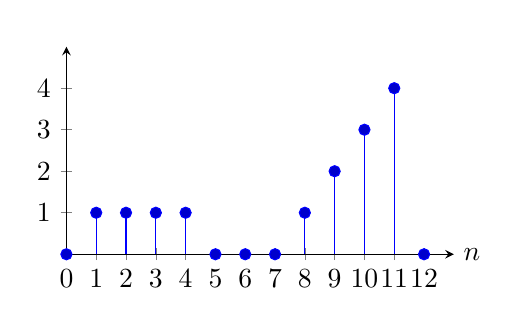
\begin{tikzpicture}
\begin{axis} [width=185pt,height=120pt,
	axis x line=bottom, 
	axis y line=middle, 
	tick align=center,
	every axis x label/.style={at={(current axis.right of origin)},anchor=west},
	every axis y label/.style={at={(current axis.above origin)}, anchor=north east,above=0mm},
	xmin=0, xmax=13,
	xtick={0,...,12},
	xlabel=$n$,
	ymin=0, ymax=5,
	ytick={0,...,4},
	ylabel={$\boldimgworld$}]
\addplot+[ycomb] 
coordinates {(0,0) (1,1) (2,1) (3,1) (4,1) (5,0) (6,0) (7,0) (8,1) (9,2)  (10,3)  (11,4)  (12,0)};
\end{axis}
\end{tikzpicture}
&~
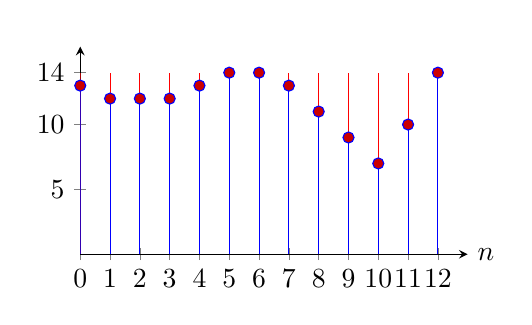
\begin{tikzpicture}
\begin{axis} [width=185pt,height=120pt,
	axis x line=bottom, 
	axis y line=middle, 
	tick align=center,
	every axis x label/.style={at={(current axis.right of origin)},anchor=west},
	every axis y label/.style={at={(current axis.above origin)}, anchor=north east,above=0mm},
	xmin=0, xmax=13,
	xtick={0,...,12},
	xlabel=$n$,
	ymin=0, ymax=16,
	ytick={0,5,10,14},
	ylabel={$\boldimgsensor$}]
\addplot[ycomb,red] 
coordinates {(0,14) (1,14) (2,14) (3,14) (4,14) (5,14) (6,14) (7,14) (8,14) (9,14)  (10,14)  (11,14)  (12,14)};
\addplot+[ycomb,blue,fill=blue,mark=*] 
coordinates {(0,13) (1,12) (2,12) (3,12) (4,13) (5,14) (6,14) (7,13) (8,11) (9,9)  (10,7)  (11,10)  (12,14)};
\end{axis} 
\end{tikzpicture}
\end{array}
$
%\end{center}
}
\caption{Pinspeck camera. (left) Input 1D signal, $\boldimgworld$. (right) The output of a pinspeck camera, $\boldimgsensor$.} 
\label{fig:pinspeck_output_plot}
\end{figure}

The output is now a signal with a wide dynamic range (a max value of 14, which correspond to the sum of the values in $\boldimgworld$) and with fluctuations due to the shadow of the occluder on the camera sensor. If there was no occluder, then the output would be a constant signal of value 14. In red we show the effect of the shadow, which is the light missing because of the presence of the occluder. You can see how the missing signal is identical to the output of the two-pixel wide pinhole camera but reversed in sign.


%\begin{figure}
%\centerline{
%\sublabel{a}{\includegraphics[width=0.45\linewidth]{figures/imaging/ph3.pdf}}}
%\centerline{
%\sublabel{b}{\includegraphics[width=0.45\linewidth]{figures/imaging/amat31.pdf}}
%\sublabel{c}{\includegraphics[width=0.45\linewidth]{figures/imaging/amat34.pdf}}
%}
%\caption{
%(a) An edge camera (b) Visualization of idealized imaging matrices:  The imaging matrix relating scene intensities to sensor readings; the inverse of that matrix;  the regularized inverse.  (c) A blurred edge imaging matrix, and its inverse and regularized inverse }
%\label{fig:amats3}
%\end{figure}





\subsection{Corner Camera}  

To show a real-world example of a more general imager, let us consider the {\bf corner camera}\index{Camera!Corner camera} \cite{Bouman17}.  This is similar to the edge
camera of \eqn{\ref{eq:edge}} and \fig{\ref{fig:amats3}}, but with
slightly more complicated geometry.  As shown in
\fig{\ref{fig:ccmodel}}{a}, a vertical edge partially blocks a scene from view, creating intensity variations on the ground, observable by viewing those intensity variations from around the corner.


\begin{figure}[t]
\centerline{
\sublabel{a}
{\includegraphics[width=0.4\linewidth]{figures/imaging/cornercam.pdf}}
\sublabel{b}
{\includegraphics[width=0.4\linewidth]{figures/imaging/cornerKey.pdf}}}
\caption{The corner camera \cite{Bouman17}.  (a) Objects, such as the cylinders labeled A and B, hidden behind a corner from a camera nonetheless cause a very small intensity differences in the ambient illumination falling on the ground.
%, observable from the camera as a very small change in the light intensity reflecting from the ground.  The image reconstruction operation is analogous to that for the edge camera of \fig{\ref{fig:amats3}}:  we subtract the reflected intensities observed at one orientation angle, say $\theta_A$ from those observed at another, say $\theta_B$. 
(b) the spatial mask is multiplied by the observed reflected ground image.}
\label{fig:ccmodel}
\end{figure}


In practice, we will subtract a mean image from our observations of the ground plane, so in the rendering equation below, we will only consider components of
the scene that may change over time, under the assumption that what we want to image behind the corner (e.g., a person) is moving.  We will call these intensities
$S(\phi, \theta)$ ($S$ for the subject), where $\phi$ measures
vertical inclination and $\theta$ measures azimuthal angle, relative to position where the vertical edge intersects the ground plane.  Integrating the light intensities falling on the ground plane, the
observed intensities on the ground will be $\boldimgground (r, \theta)$, where the
polar coordinates $r$ and $\theta$ are measured with respect to the corner.
Assuming Lambertian diffuse reflection from the ground plane, we have, for the observed intensities $\boldimgground (r, \theta)$,
\begin{equation}
 \boldimgground (r, \theta) = \int_{\phi=0}^{\phi=\pi} \int_{\xi=0}^{\xi=\theta}
 \cos(\phi) S(\phi, \xi) \mbox{d} \phi \mbox{d} \xi,
\label{eq:corner}
\end{equation}
where the $\cos(\phi)$ term in \eqn{\ref{eq:corner}} follows from the equation for surface reflection, \eqn{\ref{eq:lambert}}.



The dependence of the observation, $\boldimgground$, on vertical variations in
$S(\phi, \theta)$ is very weak, just through the $\cos(\phi)$ term.
We can integrate over $\phi$ first, to form the 1D signal,
$\imgworld (\xi)$:
\begin{equation}
  \imgworld (\xi) = \int_{\phi=0}^{\phi=\pi} 
  \cos(\phi) S(\phi, \xi) \mbox{d} \phi 
\label{eq:xcorner}
\end{equation}

Then, to a good approximation, \eqn{\ref{eq:corner}} has the form,
\begin{equation}
 \boldimgground (r, \theta) \approx \int_{\xi=0}^{\xi=\theta}
 \imgworld (\xi) \mbox{d} \xi,
\label{eq:corner1d}
\end{equation}
where $\imgworld (\xi)$ is a 1D image of the scene around the corner from the vertical edge.

\Fig{\ref{fig:ccmodel}} shows the corner camera geometry for a three-dimensional (3D) scene.  \Fig{\ref{fig:ccmodel}}{a} shows two objects, such as the cylinders labeled A and B, hidden behind a corner from a camera. Despite being behind the corner they cause a very small intensity differences in the ambient illumination falling on the ground, observable from the camera as a very small change in the light intensity reflecting from the ground. Can we reconstruct the scene hidden behind the corner using just the intensities observed on the ground? The image reconstruction operation is analogous to that for the edge camera of \fig{\ref{fig:amats3}}:  we subtract the reflected intensities observed at one orientation angle, say $\theta_A$ from those observed at another, say $\theta_B$. 

If we sample \eqn{\ref{eq:corner1d}} in its continuous variables, we
can write it in the form $\boldimgground = \mathbf{A} \boldimgworld$.  Solving \eqn{\ref{eq:deriv2}}
for the multiplier to apply to $\boldimgground$ to estimate $\boldimgworld$ yields the form shown in
\fig{\ref{fig:ccmodel}}{b}.  \Fig{\ref{fig:ccmodel}}{b} shows the spatial mask to be multiplied by the observed reflected ground image, with the result summed over all spatial pixels in order to estimate the light coming from around the corner at one particular orientation angle relative to the corner, in this case approximately 45 degrees. We see that the way to read the 1D signal from the ground plane is to take a derivative with respect to angle.  This makes intuitive sense, as the light intensities on the ground integrate all the light up to the angle of the vertical edge.  To find the 1D signal at the angle of the edge, we ask, ``What does one pie-shaped ray from the wall see that the pie-shaped ray next to it doesn't see?''


It can be shown \cite{Bouman17} that the image intensities from around-the-corner scenes introduce a perturbation of about $\frac{1}{1,000}$ to the light reflected from the ground from all sources.   
By averaging image intensities over the appropriate pie-shaped regions on the ground at the corner (\fig{\ref{fig:ccmodel}}[b]), one can extract a 1D image as a function of time from the scene around the corner.  \Fig{\ref{fig:cctraces}} shows two 1D videos reconstructed from one (\fig{\ref{fig:cctraces}}[a]) and two (\fig{\ref{fig:cctraces}}[b]) people walking around the corner.  By processing videos of very faint intensity changes on the ground, we can infer a 1D video of the scene around the corner.  The image inversion formulas were derived using inversion methods very similar to \eqn{\ref{eq:deriv2}}.  The corner camera is just one of the many possible instantiations of a computational imaging system.


\begin{figure}[t]
\centerline{
\includegraphics[width=0.9\linewidth]{figures/imaging/corner_camera_3D.eps}
}
%\centerline{
%\sublabel{a}
%{\includegraphics[width=0.4\linewidth]{figures/imaging/corner.jpg}}
%\sublabel{b}
%{\includegraphics[width=0.4\linewidth]{figures/imaging/2people.jpg}}}
%\centerline{
%\sublabel{c}
%{\includegraphics[width=0.2\linewidth]{figures/imaging/cctrace.pdf}}
%\sublabel{d}
%{\includegraphics[width=0.2\linewidth]{figures/imaging/cctrace2.pdf}}
%}
\caption{Outdoor corner camera \cite{Bouman17} experiments. (a) Camera recording ground plane intensities.  (b) Two people walking around the corner, hidden from direct view of the camera. (c) Corner camera trace with one person moving. (d) Corner camera trace with two people moving.  Angle from the corner is plotted vertically, and time is plotted horizontally.}
\label{fig:cctraces}
\end{figure}

\marginnote{People moving out of view around a corner cause small, invisible changes in the light reflecting from the ground. These faint changes occur at nearly every corner and can be used to read-out 1D images of the people around the corner.}[0in]


%% 
%% \subsection{Pinhole lightfield imager}
%% An array of pinholes.  How to construct and photograph that?
%% 


\section{Concluding Remarks}  
Treating cameras as general linear systems allows for the machinery of linear algebra to be applied to camera design and processing.  We reviewed several simple camera systems, including cameras utilizing pinholes, pinspecks, and edges to form images.
 % Bill

%% jan. 4, 2011  items to fix:
%% notation for math and reference to images.
%% how include eps figures.
%% make all the little figures (search for eps) in a common, nice matlab way for the
%% example filtering operations.

%\setcounter{chapter}{5}
\chapter{Color}
\label{chapter:color}

%\reviewcomment{Figures need reformating.}

\section{Introduction}

There are many benefits to sensing color.  Color differences let us
check whether fruit is ripe, tell whether a child is sick by looking
at small changes in the color of the skin, and find objects in
clutter.  

We'll begin our study of color by describing the physical properties of light that lead to the perception of different colors.  Then we'll describe how humans and machines sense colors, and how to build a system to match the colors perceived by an observer.  We'll briefly describe how to represent color--different color coordinate systems.  Finally, we'll describe how spatial resolution and color interact.


\section{Color Physics}


Isaac Newton revealed several intrinsic
properties of light in experiments summarized by his drawing in
\fig{\ref{fig:prism}}. A pinhole of sunlight enters through the
window shade, and a lens focuses the light onto a prism.  The prism
then divides the white light into many different colors.  These
colors are elemental: if one of
the component colors is passed through a second prism, it doesn't
split into further components.


\begin{figure}[htpb!]
\centerline{
\includegraphics[width=.9\linewidth]{figures/color/newtonDrawing.jpg}
}
\caption{Isaac Newton's illustration of experiments with light \cite{Fara2015}.  White
light enters from a hole in the window shade at the right, where it is
focused with a lens and then passes through the first
prism.  The prism separates the white light into different colors by
bending each color a different amount.  The second prism in the
drawing demonstrates that those colors are elemental:  as an individual
color passes through the second prism, the light doesn't break into
other colors.}
\label{fig:prism}
\end{figure}


Our understanding of light and color explains such experiments.  Light
is a mixture of electromagnetic waves of different wavelengths.
Sunlight has a broad distribution of
light of the visible wavelengths.  At an air/glass interface, light
bends in a wavelength-dependent manner, so a prism disperses the
different wavelength components of sunlight into different angles, and
we see different wavelengths of light as different colors.  
Our eyes are sensitive to only the narrow band of that electromagnetic
spectrum, the visible light, from approximately 400 nm 
to 700 nm, which appears blue to deep red, respectively.




The bending of light at a material boundary is called {\bf refraction}, and
its wavelength dependence lets the prism separate white light into its
component colors.  A second way to separate light into its spectral
components is through {\bf diffraction}, where constructive
interference of scattered light occurs in different directions for
different wavelengths of light. 
\marginnote{Newton understood that white light could be decomposed into different colors and invented the term {\bf spectrum}.}

\Fig{\ref{fig:colorWavelengths}}{a} 
shows a simple spectrograph, an apparatus to reveal the spectrum of light, based on
diffraction from a compact disk (CD) \cite{spectrometer}.  Light passes through the slit at
the right, and strikes a CD (with a track pitch of about 1,600 nm).
Constructive interference from the light waves striking the CD tracks
will occur at a different angle for each wavelength of the light, yielding
a separation of the different wavelengths of light according to their
angle of diffraction.  The diffracted 
light can be viewed,   \fig{\ref{fig:colorWavelengths}}{b}, 
or photographed through the hole at the bottom
left of the photograph.  The spectrograph gives an immediate visual
representation of the spectral components of colors in the world. Some examples are shown in \fig{\ref{fig:examples1}}.



\begin{figure}[t]
\centerline{
\includegraphics[width=1.0\linewidth]{figures/color/cd_spectrometer_setup.eps}
}
%\centerline{
%\sublabel{a}{\epsfig{file=figures/color/cdSpectrograph.eps,width=3in}}
%\sublabel{a}{\epsfig{file=figures/color/spectrometer2.jpg,width=3in}}
%\sublabel{b}{\epsfig{file=figures/color/rainbow.eps,width=1.5in}}}
\caption{(a) A simple spectrograph.
  Slit at right accepts light from primarily one object in the world.
  Light diffracted by the CD is viewed from the hole at the bottom
  left.  (b) The bending by diffraction is wavelength dependent, and the
  light from a given direction is broken into its spectral components. We indicate the location of the CD in the picture just in case our youngest readers have not seen one.}
\label{fig:colorWavelengths}
\end{figure}




\begin{figure}
\centerline{
\includegraphics[width=1.0\linewidth]{figures/color/lightspectra_objects.eps}
}
%\sublabel{a}{\centerline{
%\epsfig{file=figures/color/DSC00780.jpg,width=1.7in}
%\epsfig{file=figures/color/leafspec.eps,width=1.05in}
%}}
%\sublabel{b}{\centerline{
%\epsfig{file=figures/color/reddoor.eps,width=1.3in}
%\epsfig{file=figures/color/reddoorspec.eps,width=1.6in}
%}}
%\sublabel{c}{\centerline{
%\epsfig{file=figures/color/fourlamp.eps,width=1.7in}
%\epsfig{file=figures/color/neon.eps,width=1.5in}}}
\caption{The light spectra from some everyday objects, analyzed by the spectrograph of
  \fig{\ref{fig:colorWavelengths}}.  (a) A leaf, with some
  yellowish highlights, shows primarily green, with a little red (red
  and green can combine to appear yellow).  (b) A
  red door.  (c)  A fluorescent light (when turned on) shows the discrete spectral wavelengths at
  which the gas fluoresces.
}
\label{fig:examples1}
\end{figure} 


\subsection{Light Power Spectra}

The light intensity at each wavelength is called the {\bf power spectrum} of the
light.  The color appearance of light is determined by many factors, including the image context in which the light is viewed; but a very important factor in determining color appearance is the power spectrum. In this initial discussion of color, we will assume that the power spectrum of light determines its appearance, although you should remember that this is true only within a fixed visual context.

\marginnote{Why does the sky look blue? And why does it look orange during a sunset? 
\\[6pt]
\centerline{
\includegraphics[width=.4\linewidth]{figures/color/sunset_key_west.jpg}
}
}[-1.6in]

\Fig{\ref{fig:examples1}} shows a spectrograph visualization of some light power spectra (the right image of each row) along with the image that the spectrograph was pointed toward (left images).
\Fig{\ref{fig:sources}} shows the spectrum of a blue sky, plotted as 
intensity as a function of wavelength.



\begin{figure}
\centerline{
\includegraphics[width=0.7\linewidth]{figures/color/Spectrum_of_blue_sky.eps}
%\epsfig{file=figures/color/blueSky.jpg,width=3in}
~~~~~
\includegraphics[width=.15\linewidth]{figures/color/IMG_0122.jpg}
}
\caption{Power spectrum of blue skylight \cite{blueskyWiki}.}
\label{fig:sources}
\end{figure}


\subsection{The Color Appearance of Different Spectral Bands}

It is helpful to develop a feel for the approximate color appearance of different
light spectra.  Again, we say the approximate appearance because the subjective appearance can change according to other factors than just the spectrum.

The visible spectrum lies roughly in the range between 400 and 700 nm,
see \fig{\ref{fig:rainbow}}.  We can divide the visible spectrum into
three 100 nm bands, and study the appearance of light power
spectra where power is present or absent from each of those three
bands, in all of the eight ($2^3$) possible combinations.


\begin{figure}
\centerline{
\epsfig{file=figures/color/rainbow3.eps,width=5in}}
\caption{The approximate color appearance of light over different
  spectral regions.}
\label{fig:rainbow}
\end{figure}

Light with spectral power distributed in just the 400--500 nm
wavelength band will look some shade of blue, the exact hue depending
on the precise distribution.  Light in the 500--600 nm band will
appear greenish.  Most distributions within the 600--700 nm band will
look red.

White light is a mixture of all spectral colors.  A spectrum of light
containing power evenly distributed over 400---700 nm would appear approximately
white.  Light with no power in any of those three bands, that is, 
darkness, appears black.

There are three other spectral classes left in this simplified grouping
of spectra:  spectral power present in two of the spectral
bands, but missing in the third.
Cyan is a combination of both blue and green, or roughly spectral
power between 400 and 600 nm.  In printing and color film
applications, this is sometimes called {\em minus red}, since it is the
spectrum of white light, minus the spectrum of red light.  The blue
and red color blocks, or light in the 400--500 nm band, and in the
600--700 nm band, is called magenta, or minus green.  Red and green together,
with spectral power from 500--700 nm, make yellow, or minus blue (\fig{\ref{fig:names}}). 

\begin{figure}
\centerline{
\includegraphics[width=1.0\linewidth]{figures/color/cartoonColor2.eps}
}
%\epsfig{file=figures/color/cartoonColor2.eps,width=5in}}
\caption{For coarse orientation only, this cartoon model gives the color appearance of different spectral bands of the spectrum of visible light.}
\label{fig:names}
\end{figure}



\subsection{Light Reflecting from Surfaces}

When light reflects off a surface, the power spectrum alters in ways that depend on the surface’s characteristics and geometry. These
changes in light allow us to perceive objects and surfaces by observing their influence on the reflected light.

The interaction between light and a surface can be quite complex. Reflections can be specular or diffuse, and the reflected
power spectrum may depend on the relative orientations of the incident
light, surface, and the observed reflected ray. In its full generality, the reflection of light from a surface is described by the
bidirectional reflectance distribution function (BRDF) \cite{Nicodemus1965,Matusik2002}.
For this discussion, we will focus on diffuse
surface reflections, where the power spectrum of the reflected light, $r(\lambda)$,
is proportional to the wavelength-by-wavelength product of the power
spectrum of the incident light, $\imgin (\lambda)$, and a {\bf reflectance
  spectrum}, $s(\lambda)$, of the surface:
\begin{equation}
r(\lambda) = k \imgin (\lambda) s(\lambda),
\end{equation}
where the proportionality constant $k$ depends on the reflection geometry.
This diffuse reflection model characterizes
most matte reflections.  Such wavelength-by-wavelength scaling
is also a good model for the spectral changes to light caused by transmission
through an attenuating filter.  The incident power spectrum is
then multiplied at each wavelength by the {\bf transmittance spectrum} of
the attenuating filter.

Some reflectance spectra of real-world surfaces are plotted in
\fig{\ref{fig:sourcerefl}}.  The flower {\em Hepatica Nobilis} (solid line) is blue, while {\em Pyrostegia venusta} (dotted line) is orange.

\begin{figure}[t]
\centerline{
\includegraphics[width=1.0\linewidth]{figures/color/flowerSpectra.eps}
}
%\centerline{
%\sublabelnp{(a) reflectance functions of two flowers}{\epsfig{file=figures/color/flowerSpectra.jpg,width=3in}}
%\sublabelnp{(b) Hepatica nobilis (solid line)}{\epsfig{file=figures/color/nobilis.jpg,width=1.3in}}
%\sublabelnp{(c) Pyrostegia venusta (dotted line)}{\epsfig{file=figures/color/Pyrostegia_venusta3.jpg,width=1.3in}}
%}
\caption{Reflectance spectra from two flowers \cite{Arnold2010}. The blue {\em Hepatica nobilis} flower \cite{nobilis} and the orange flower, {\em Pyrostegia venusta} \cite{venusta}.}
\label{fig:sourcerefl}
\end{figure}




The reflectance spectrum of a surface often carries valuable information about the material being viewed, such as whether a fruit is ripe, whether a human's skin is healthy, or whether the material differs from another viewed material.  It may be the case that a low-dimensional version of the surface reflectance spectrum is sufficient for many visual tasks, and as we see subsequently, the human visual system represents color with only three numbers.  So it is an important visual task to estimate either the surface reflectance spectrum, or a low-dimensional summary of it. 


To estimate surface colors by looking, a vision system has the task of estimating the illumination spectrum and the surface reflectance spectra, from observations of only their products.
When the illumination is white light with equal power in all spectral bands,
the observed reflected spectrum is proportional to the reflectance spectrum of the
material itself.  However, under the more general condition of unknown illumination color, a visual system will need to estimate the surface reflectance spectrum, or projections of it, by taking the context of nearby image information into account.

There are many proposed algorithms to do that, ranging from heuristics, for example, assuming the color of the brightest observed object is white \cite{McCann76}, to statistical methods \cite{Brainard97} and neural network based approaches \cite{Barron2015}.
Even humans don't solve the problem perfectly or consistently, revealed especially through the internet meme of \#TheDress \cite{Bleasdale2015}, 
%``TheDress'', 
shown in \fig{\ref{fig:thedress}}.  


\begin{figure}[t]
\centerline{
%\sublabel{a}{\epsfig{file=figures/color/thephotoofthedress.jpg, width=1.9in}}
%\sublabel{b}{\epsfig{file=figures/color/gr2_lrg.jpg, width=2.9in}}
\sublabel{a}{\includegraphics[width=1.9in]{figures/color/thephotoofthedress.jpg}}
\sublabel{a}{\includegraphics[width=2.9in]{figures/color/gr2_lrg.jpg}}
}
\caption{(a) \#The Dress, photographed and posted by \cite{Bleasdale2015}, reprinted with permission.  (b) The spectra of the light we see is the product of an assumed illumination spectrum and the inferred surface reflectance spectra.  If people make different assumptions about the illumination, they can perceive different colors within the same image, as shown in this illustration \cite{Brainard2015}.  Reprinted with permission from Elsevier.
}
\label{fig:thedress}
\end{figure}



The perceived colors of the dress depend on the assumed color of the illumination, and people can disagree significantly about the colors they see \cite{Brainard2015}.  The assumption of a warm, yellowish, illumination color leads to a perception of blue and black material.  The assumption of a cool, blueish illumination leads to a perception of white and gold material.  Both perceptions are consistent with the observed product of illumination and reflectance  seen in the dress image.  

\marginnote{Did you perceive the dress, \fig{\ref{fig:thedress}}, to be black on blue, or gold on white?  Can you make the perception change?}

While such context-dependent effects are important in color perception, as we quantify color perception we will assume that our perception of color depends only on the spectrum of light entering the eye.  This will serve us well for many industrial applications.


\section{Color Perception}

Now we turn to our perception of color.  We first describe the
machinery of the eye, then describe some methods to measure color appearance.  These methods to measure color appearance implicitly assume a white illumination spectrum, but they often serve the needs of industry and science.


\subsection{The Machinery of the Eye}

%Figure~\ref{fig:ramon}~a is a drawing \cite{cajal1904} of the photoreceptors, called the rod and cones, in the retina of the eye.  The tall receptors are the rods, used in low-light levels, and the short ones are the cones, used in color vision.  Interestingly, the light enters from the bottom of the drawing, passing through the nerve fibers and blood vessels before reaching the photosensitive detectors at the top of the image. 



An instrument such as a spectrograph (\fig{\ref{fig:colorWavelengths}} shows a simple one)
can measure the light power spectrum at hundreds of
different wavelengths within the visible band, yielding hundreds of
numbers to describe the light power spectrum.  Despite this, a useful
description of the visual world can be obtained from a much lower
dimensional description of the light power spectrum.  
\marginnote{The retina contains photoreceptors called the rod and cones. Rods are used in low-light levels, and the cones are used in color vision. In low-light, only the rods operate and our vision becomes black and white.}

The human visual
system analyzes the incident light power spectrum with only three
different classes photoreceptors, called the L, M, and S cones because
they sample at the long, medium, and short wavelengths.  This gives
the human visual system a three-dimensional (3D) description of light, with
each photoreceptor class taking a different weighted average of the
incident light power spectrum.

\Fig{\ref{fig:ramon}}{a} shows 
the spatial sampling pattern, for each of the three cone classes, measured from a subject's eye \cite{Hofer2005}. The L cones are
colored red, the M cones green, and the S cones are colored
blue. Note the hexagonal packing of the cones in the retina, and the
stochastic assignment of L, M, and S cones over space.  Note also the much sparser spatial sampling of the S cones than of either the L or M cones.
\Fig{\ref{fig:ramon}}{b} shows the spectral sensitivity curves
for the L, M, and S cones.  This sampling pattern was measured from near the {\bf fovea}, where there are no rods, and the cones are close-packed.


\begin{figure}[t]
\centerline{
%\sublabel{a}{\epsfig{file=figures/color/ramonycajal,width=2in}}
\sublabel{a}{\epsfig{file=figures/color/YYretina.pdf,width=2in}}
\sublabel{b}{\epsfig{file=figures/color/Cones_SMJ2_E.jpg,width=2.5in}}
}
%\centerline{
%\sublabel{c}{\epsfig{file=figures/color/Cones_SMJ2_E.jpg,width=4in}}
%}
\caption{
%(a) Drawing of the eye's photoreceptors by the physiologist Ramon y Cajal \cite{cajal1904}.
 (a)  Measured cone receptor classes and positions in a human retina, with cone receptor classes shown as red, green, and blue (subject YY, redrawn from \cite{Hofer2005}).
(b) Photoreceptor sensitivities as a function of light wavelength  \cite{Vanessaezekowitz2007}.}
\label{fig:ramon}
\end{figure}


We can describe the photoreceptor responses using matrix algebra.
If the matrix $\mathbf{C}_{\mbox{eye}}$ consists of the spectral sensitivities of the
L, M, and S cones in three rows, and the vector $\mathbf{t}$ is a column
vector of the spectrum of light incident on the eye, then the L, M,
and S cone responses will be the product,
\begin{equation}
    \begin{bmatrix}
    L  \\
    M  \\
    S \\
    \end{bmatrix}
= \mathbf{C}_{\mbox{eye}} \, \mathbf{t}
\label{eq:lmsct}
\end{equation}

The fact that our eyes have three different classes of photoreceptors
has many consequences for color science.  It determines that there are
three primary colors, three color layers in photographic film, and
three colors of dots needed to render color on a display screen.  In
the next section, we describe how to build a color reproduction system that matches the colors seen in the world by a human observer.

%% \billf{Who first discovered trichromaticity, and how?}


\subsection{Color Matching}

Color science tells us how to analyze and reproduce color.
We seek to build image displays so that the output colors match those of
some desired target, and to manufacture items with the same colors over
time.  Much of the color industry revolves around the ability to repeatably control colors.
Colors can be trademarked (Kodak Yellow, IBM Blue) and we have
color standards for foods.  \Fig{\ref{fig:french}} shows French fry color
standards.

\begin{figure}[t]
\centerline{
\epsfig{file=figures/color/munsell.jpg,width=3.5in}}
\caption{The USDA color standards for French fried potatoes, one of
  many color standards \cite{Munsell2020}.} 
\label{fig:french}
\end{figure}

One of the tasks of color science is to predict when a person will
perceive that two colors match.  For example, we
want to know how to adjust a display to match the color
reflecting off some colored surface.  Even though the spectra may be
very different, the colors can almost always be made to match.

It is possible to infer human color matching performance by examining the spectral sensitivity curves of the receptors shown in \fig{\ref{fig:ramon}}{b}. We attempt to match a color using a combination of reference colors, typically called primary colors. Through experimentation, it has been discovered that the appearance of any color can be matched through a linear combination of three primary colors. This is due to the presence of three classes of photoreceptors in our eyes. It has also been found that these color matches are transitive—if color A matches a particular combination of primaries and color B matches the same combination of primaries, then color A will match color B. Consequently, the amount of each primary required to match a color can serve as a set of coordinates indicating color \cite{Wandell95}.

\subsection{Color Metamerism}


Two different spectra are metameric if they appear to be the same color to our eyes.
There is a large space of metamers:  any two 
vectors describing light power spectra
that give the same projection onto a set of color matching functions
will look the same to our eyes.  There's a high-dimensional space of light spectra, and we're
only viewing projections onto a 3D subspace in the colors we see.\marginnote{Do spotlights on produce in a supermarket help good and bad fruit become metameric matches?}

In practice, the three projections we observe capture much of the interesting action in images.  Hyperspectral images (recorded at many different wavelengths of analysis) add some, but not
a lot, to the image formed by our eyes.



\subsection{Linear Algebraic Interpretation of Color Matching}


% \begin{figure}
% \centerline{
%\epsfig{file=figures/color/conditions.jpg,width=4in}
%\epsfig{file=figures/color/conditionsForMatch.jpg,width=4in}
% }
% \caption{Conditions for a perceptual match for the system of Fig.~\ref{fig:colorsystem}.  First, $\mathbf{C}$ must be a linear combination of the spectral sensitivities of the photoreceptors in the eye, thus $\mathbf{C} = \mathbf{R} \mathbf{C}_{\mbox{eye}}$, for some full-rank, 3x3 matrix, $\mathbf{R}$.  Second, the light sensor spectra, in the rows of $\mathbf{C}$, and the display element spectra, in the columns of $\mathbf{P}$, must satisfy $\mathbf{C}\mathbf{P} = \mathbf{I}_{\mbox{3}}$.}
% \label{fig:conditions}
% \end{figure}

In this chapter, we assume that color appearance is determined by the light spectrum reaching the eye. In reality, numerous factors can influence color appearance, including the eye's state of brightness adaptation, ambient illumination, and surrounding colors. However, a color matching system that relies solely on the light spectrum will still perform well.

To measure the color associated with a light spectrum $\mathbf{t}$ we need to be able to predict the eye's responses to the spectrum.
From \eqn{\ref{eq:lmsct}}, the task of color measurement is to find the projection of a given light spectrum into the
special 3D subspace defined by the eye's cone spectral response curves.
Any basis for that 3D subspace will serve that task, so the three basis
functions do not need to be the color sensitivity curves of
\fig{\ref{fig:ramon}} themselves.  They can be any linear combination
of them, as well. 

We can define a {\bf color reproduction system}, \fig{\ref{fig:colorsystem}}, by first specifying its  three spectral sensitivity curves.  We put these into the $3 \times N$ matrix, $\mathbf{C}$, where $N$ is the number of spectral samples over the visible illumination range.  As discussed previously, the three curves, $\mathbf{C}$, should be a linear combination of the eye's spectral sensitivity curves, or
\begin{equation}
    \mathbf{C} = \mathbf{R} \, \mathbf{C}_{\mbox{eye}},
    \label{eq:match2}
\end{equation}
where $\mathbf{R}$ is any full-rank $3 \times 3$ matrix. We can translate between any two different color
spaces by  applying a general $3 \times 3$ matrix transformation
to change basis vectors.  Note, the basis vectors do not need to be
orthogonal, and  most color system basis vectors are not.


\begin{figure}[t]
\centerline{
\includegraphics[width=1.0\linewidth]{figures/color/colorRepro2.pdf}
}
%\centerline{
%% \epsfig{file=figures/color/colorsystem.jpg,width=5in}}
%\epsfig{file=figures/color/colorRepro.jpg,width=5in}}
\caption{A color reproduction system.  Light sensors a, b, and c respond to the input light spectrum $\mathbf{t}$, giving sensor activations $\mathbf{C} \mathbf{t}$.  Combinations of those activations drive the display elements d, e, and f, producing the output spectrum $\mathbf{P}\mathbf{M} \mathbf{C} \mathbf{t}$. Conditions on $\mathbf{P}$, $\mathbf{M}$, and $\mathbf{C}$ can ensure that the input and output colors match for an observer.}
\label{fig:colorsystem}
\end{figure}


\subsection{Color Matching Functions and Primary Lights}

A  color reproduction system measures an input light and produces an output light that matches the color appearance of the input light.  A camera with a screen display is an example of a color reproduction system, as the colors of objects in the world are measured, then reproduced on the screen display of the camera.  
We can match the eye's response to a given light spectrum through the appropriate control of a sum of three lights, which we'll call the {\bf primary lights}\index{Color!Primary colors}. For the example of a display screen, the three color elements of each pixel are the primary lights.  

Because the eye's photosensors respond in linear proportion to the amount of the incoming light spectrum within its spectral sensitivity curve, the rules of linear algebra apply to color manipulation.  For a given set of three primary lights, the strengths of each primary light can be adjusted to obtain a visual match to a desired color.  There is one exception to this: because primary lights can only be combined in positive values, some input colors are outside the {\bf gamut}---the range of colors that can be produced---of a the positive combination of a given set of primary lights.

The color reproduction system is then defined by two sets of spectral curves and a $3 \times 3$ matrix, $\mathbf{M}$, see \fig{\ref{fig:colorsystem}}.  The first set are the spectral sensitivities as a function of wavelength for each of the three photosensors.  We write each of those spectral curves as a row vector of a matrix, $\mathbf{C}$.  The $3 \times 3$ matrix, $\mathbf{M}$, translates any color measurement to a set of amplitude controls for the primary lights, $\mathbf{P}$. The second set of spectral curves of a color reproduction system are the spectra of the three primary lights, which we write as column vectors of the matrix, $\mathbf{P}$.

For a given set of primary lights, $\mathbf{P}$, we seek to find a matrix of color sensitivity curves, $\mathbf{C}$, and $3 \times 3$ matrix, $\mathbf{M}$, which allow perfect reproduction of colors, as viewed by a human observer.  Here, we derive the conditions
%, given in \fig{\ref{eq:conditions}}, 
that $\mathbf{P}$,  $\mathbf{C}$, and $\mathbf{M}$ must satisfy to allow for perfect reproduction of colors.

Let the spectrum of the light reflecting from the surface to be matched in color be $\mathbf{t}$.  The eye's response to that light is modeled as the sum of a term-by-term multiplication of the spectral sensitivities of each photoreceptor, in the rows of $\mathbf{C}_{\mbox{eye}}$ times the spectrum of the light.  Thus, the responses of the eye to that spectrum will be the $3 \times 1$ column vector, $\mathbf{C}_{\mbox{eye}} \mathbf{t}$.  

We can write the response of the eye to the {\em output} of the color matching system as the following matrix products.  The light impinging on the sensors (a, b, c in \fig{\ref{fig:colorsystem}}) of the color matching system will give responses $\mathbf{C} \mathbf{t}$ and controls  $\mathbf{M} \mathbf{C} \mathbf{t}$ to the primary lights.  If this output modulates the corresponding primary lights (d, e, and f in \fig{\ref{fig:colorsystem}}), then the light displayed by the color matching system will be $\mathbf{P} \mathbf{M} \mathbf{C} \mathbf{t}$.  We want this spectrum to give the same responses in the eye as the original reflected color, thus we must have:
$\mathbf{C}_{eye} \mathbf{P} \mathbf{M} \mathbf{C} \mathbf{t} = \mathbf{C}_{eye} \mathbf{t} $.  Because that relation must hold for {\em any} input vector $\mathbf{t}$, we must have
\begin{equation}
\mathbf{C}_{eye} \mathbf{P} \mathbf{M} \mathbf{C}  = \mathbf{C}_{eye}   
\label{eq:match}
\end{equation}

What conditions on $\mathbf{P}$ and $\mathbf{C}$ are required for \eqn{\ref{eq:match}} to hold?  First, the subspace of the eye responses $\mathbf{C}_{eye}$ must be the same as that measured by the color sensing system, $\mathbf{C}$.  If that weren't the case, 
then perceptibly different spectra could map onto the same color sensing system measurements. So we must have $\mathbf{C} = \mathbf{R} \mathbf{C}_{eye}$, for some full-rank $3 \times 3$ matrix, $\mathbf{R}$ (with inverse $\mathbf{R}^{-1}$).  Substituting this twice into \eqn{\ref{eq:match}} gives
\begin{equation}
\mathbf{R}^{-1} \mathbf{C} \mathbf{P} \mathbf{M} \mathbf{R} \mathbf{C}_{eye} = \mathbf{C}_{eye}
\label{eq:match2}
\end{equation}
From \eqn{\ref{eq:match2}} it follows that  $\mathbf{C} \mathbf{P} \mathbf{M} = \mathbf{I}_3$, the $3 \times 3$ identity matrix.  These conditions on the spectral sensitivities, $\mathbf{C}$, the display spectra, $\mathbf{P}$ and the sensors-to-primaries mixing matrix, $\mathbf{M}$ for a color reproduction system are  summarized below:
\begin{eqnarray}
\mathbf{C} & = & \mathbf{R} \mathbf{C}_{\mbox{eye}} 
\label{eq:conditionsA} \\
\mathbf{M} & = & (\mathbf{C P})^{-1},
\label{eq:conditions}
\end{eqnarray}
where $\mathbf{C}_{\mbox{eye}}$ are the human photoreceptor sensitivities and $\mathbf{R}$ is a full-rank $3 \times 3$ matrix.  

%\marginnote{Conditions required for color matching in the color reproduction system of \fig{\ref{fig:colorsystem}}.}

\Fig{\ref{fig:exampleColor}} displays  the elements of two matrices $\mathbf{C}$ and $\mathbf{P}$ that define a valid color matching system.  For a color reproduction system to be physically realizable, the elements of the primary spectra, $\mathbf{P}$, must be non-negative.

% (In some color reproduction systems, there
% may be an additional 3x3 matrix Q multiplying the raw sensor spectral sensitivities to obtain the 
% color matching matrix C).



\begin{figure}[t]
\centerline{
\sublabelnp{(a)}{\epsfig{file=figures/color/ciergb.jpg,width=2.5in}}
\sublabelnp{(b)}{\epsfig{file=figures/color/primaryLights.jpg,width=2.5in}}}
\caption{The elements of the matrices $\mathbf{C}$ and $\mathbf{P}$ for an example color matching system.  (a) Spectral sensitivity curves, the rows of a color measurement matrix, $\mathbf{C}$. These should be linear combinations of the eye's photosensitivity curves, $\mathbf{C}_{\mbox{eye}}$.
(b) Corresponding primary lights, $\mathbf{P}$ \cite{Acdx2009},  satisfying $\mathbf{C} \mathbf{P}= \mathbf{I}_3$ ($\mathbf{M} = \mathbf{I}_3$  in equation [\ref{eq:conditions}]).}
\label{fig:exampleColor}
\end{figure}

Because many color sensitivity matrices $\mathbf{C}$ can satisfy \eqn{\ref{eq:conditionsA}} some standardized color sensitivity matrices have been adopted to allow common representations of colors. 


\subsection{CIE Color Space}

A color space is defined by the matrix, $\mathbf{C}$, with three rows
of color sensitivity functions.  These three sensitivity functions, $\mathbf{C}$, must be some linear combination of the sensitivity functions of the eye, $\mathbf{C}_{\mbox{eye}}$.
One color standard is the Commission Internationale de l'Eclairage (CIE) {\em XYZ} color space, $C_{\mbox{CIE}}$.  The CIE color matching functions, the rows of $\mathbf{C}_{\mbox{CIE}}$
were designed to be all-positive at every wavelength and are shown
in \fig{\ref{fig:ciecie}}.  


\begin{figure}[t]
\centerline{
{\epsfig{file=figures/color/ciecie.jpg,width=3in}}}
\caption{CIE color matching functions \cite{cie1931}.}
\label{fig:ciecie}
\end{figure}


An unfortunate property of the CIE color-matching functions is that no all-positive set of color primaries, $\mathbf{P}_{\mbox{CIE}}$ forms a color-matching system with those color-matching functions, $\mathbf{C}_{\mbox{CIE}}$.  But $\mathbf{C}_{\mbox{CIE}}$ is a valid matrix with which to measure colors, even though there is no physically realizable set of corresponding color primaries, $\mathbf{P}_{\mbox{CIE}}$.

To find the CIE color coordinates, one projects the input spectrum
onto the three color-matching functions, to find coordinates, called
tristimulus values, labeled $X$, $Y$, and $Z$.   Often, these values are
normalized to remove overall intensity variations, and one calculates {\bf CIE chromaticity coordinates}\index{Color!CIE chromaticity coordinates} $x = \frac{X}{X+Y+Z}$ and $y = \frac{Y}{X+Y+Z}$.



\begin{comment}
\begin{figure}[htpb!]
\centerline{
\epsfig{file=figures/color/metamerism.eps,width=6in}}
\caption{The two spectra in the figure above, from \cite{Wandell95},
  are colors that match perceptually:  daylight, and the spectrum a
  monitor adjusted to match daylight.    The figure at right shows a
  graphical rendition of the projection from the high-dimensional
  space of power spectra onto a lower-dimensional subspace,
  representing the 3D space of human color perception.  The red and
  blue dots in the higher-dimensional space are ``metameric'' in that
  they project to the same location in the lower-dimensional subspace.}
\label{fig:metamerism}
\end{figure}
\end{comment}

\begin{comment}
Let us summarize our discussion of color so far.  Under certain
viewing conditions, the perceived color depends just on the spectral
composition of light arriving at the eye (we move to more general
viewing conditions next).  Under such conditions, there is a simple
way to describe the perceived color:  project its power spectrum onto
a set of 3 vectors called color matching functions.  These projections
are the color coordinates.  
We standardize on particular sets of color coordinates.  One such set
is the CIE XYZ system.  
\end{comment}

\begin{comment}
How do you translate from one set of color coordinates
to another, say, for notation, from the color coordinates in a unprimed system to those
in a primed system?   Place the spectra of a set of primary lights
into the columns of a matrix ${\bf P}$.  If we take the color
coordinates, $\mathbf{x}$, as a 3x1 column vector and multiply them by the matrix
${\bf P}$, we get a spectrum which is metameric with the input
spectrum whose color coordinates were $\mathbf{x}$.  So to convert
$\mathbf{x}$ to its representation in a primed coordinate system, we just
have to multiply this metameric spectrum by  the color matching
functions for the primed color system:
\begin{equation}
\mathbf{x}' = {\bf C}'{\bf P} \mathbf{x}
\end{equation}
The color translation matrix ${\bf C}'{\bf P}$ is a 3x3 matrix.
\end{comment}



%% When did people learn that we have three color receptors, and how did
%% they find out?  ((   read about it.        ))



\begin{comment}

\subsection{Color mixing}

In art or photography, we often talk of ...      (relate to color primaries).


\begin{figure}[htpb!]
\centerline{
\epsfig{file=figures/color/yellowgreen.eps,width=1.5in}}
\caption{The cyan of Windex and the yellow of Joy combine to give a
 green color.}
\label{fig:colormixing}
\end{figure}

Colors and color mixing are a delightful aspect of our visual experience.
Fig.~\ref{fig:colormixing} shows an everyday example of color mixing:
yellow and cyan colors combining to give a green. 

Physically, color mixing involes combining the spectra of the two
colors to be mixed to create the power spectrum of the mixed color.
Various processes cause colors to mix, but the results
can be divided into two broad classes of mixing, called additive and
subtractive.  Under additive color mixing, the
power spectra add together to form the spectrum of the resulting
color.  This model of mixing covers the case of many small color 
elements for which the appearance is fused, such as tiny elements of a
display, or the case of several light projectors pointing at the same screen.
CRT color televisions, DLP projectors, and
colors viewed very closely in space or time all exhibit additive color
mixing.  The spectrum of the mixed color is a weighted sum of the
spectra of the individual components.  In the additive
color mixing model, red and green combine to give yellow, as can be
seen from the cartoon models of Figs.~\ref{fig:names} and
\ref{fig:colormixing}. 

A second way colors combine is called subtractive color mixing, but
might better be called multipliciative color mixing.  Under this
mixing model, the spectrum of the combined color is proportional to
the {\em product} of the mixed components.  This color mixing occurs
when light of one color reflects diffusely off a surface of another
color, or passes through a sequence of attenuating spectral filters,
such as with photographic film, paint, optical filters, and crayons.
Under the subtractive color mixing model, cyan and yellow combine to
give green, since the cyan filter attenuates the red components of
white light, and yellow filter would remove the remaining blue
components, leaving only the green spectral region of the original
white light.  Under subtractive color mixing,  red and green combine to give black.

Figure~\ref{fig:mixing} shows examples of color mixing.

\begin{figure}[htpb!]
\centerline{
\sublabel{a}{\epsfig{file=figures/color/additiveMixing.eps,width=3in}}
\sublabel{b}{\epsfig{file=figures/color/subtractiveMixing.eps,width=3in}}}
\caption{Examples of color mixing, in the world of cartoon color spectra.  (a) Additive, (b) subtractive.  The
 spectra and the resulting colors.}
\label{fig:mixing}
\end{figure}


Because the spectrum depends on surfaces, it is very useful to measure
the spectrum of reflected light, and we discuss how the eye does that
in the following section.

\end{comment}



\section{Spatial Resolution and Color}

Color interacts with our perception of spatial resolution.  For some directions in color space, the eye is very sensitive to fine spatial modulations, while for other color space directions, the eye is relatively insensitive.  Some color coordinate systems take advantage of this disparity to enable efficient representation of images by sampling image data sparsely along color axes where human perception is insensitive to blurring.

In a red-green-blue (RGB) representation, the eye is sensitive to high spatial frequency changes in both red and green, as shown in figures \ref{fig:girls1} and \ref{fig:girls2}.  A rotation of the color coordinates of the image, followed by a nonlinear stretching, can put the image into a color space called L, a, b\index{Color!Lab space}.  In that space, the eye is very sensitive to any blurring of the L color component, called luminance, but is relatively insensitive to blurring of the a or b components, as demonstrated in \fig{\ref{fig:girls3}} and \ref{fig:girls4}.  This effect is commonly exploited in image compression, allowing some image components to be sampled more coarsely than others.


\begin{figure}
\centerline{
\includegraphics[width=1.0\linewidth]{figures/color/nonblur_girls.eps}
}
%\centerline{
%\sublabelnp{(a) Original}{\epsfig{file=figures/color/nonblur.eps,width=2.3in}}
%\sublabelnp{(b) R, G, B components}{\epsfig{file=figures/color/rgbgirls.eps,width=2.3in}}
%\sublabelnp{(c) blurred R, G, B components}{\epsfig{file=figures/color/blurrgbgirls.eps,width=2.0in}}}
\caption{(a) Original image.  (b) RGB components.  (c) RGB components,
  each blurred.  These sharp and blurred components are used  in the color images of \fig{\ref{fig:girls2}}.
}
\label{fig:girls1}
\end{figure}



\begin{figure}
\centerline{
\includegraphics[width=1.0\linewidth]{figures/color/blur_rgb_girls.eps}
}
%\centerline{
%\sublabelnp{(a) R component blurred}{\epsfig{file=figures/color/blurrgirls.eps,width=2.3in}}
%\sublabelnp{(b) G component blurred}{\epsfig{file=figures/color/blurggirls.eps,width=2.3in}}
%\sublabelnp{(c) B component blurred}{\epsfig{file=figures/color/blurbgirls.eps,width=2.3in}}}
\caption{Color images composed of sharp and blurred components from figures \ref{fig:girls1}(b) and \ref{fig:girls1}(c).  (a) R component blurred, G and B components sharp.  (b)  G component blurred, R and B components sharp. (c) B component blurred, R and G components sharp. Blurring either the R or G components of the image leads to a blurry-looking full-color image.
}
\label{fig:girls2}
\end{figure}

\begin{comment}
\begin{figure}[htpb!]
\centerline{
\epsfig{file=figures/color/rgbyiq.eps,width=3in}}
\caption{Human spatial frequency sensitivity in R, G, B and L, a, b
  color representations
}
\label{fig:sensitivity}
\end{figure}
\end{comment}




\begin{figure}
\centerline{
\includegraphics[width=1.0\linewidth]{figures/color/nonblur_lab_girls.eps}
}
%\centerline{
%\sublabelnp{(a) Original}{\epsfig{file=figures/color/nonblur.eps,width=2.3in}}
%\sublabelnp{(b) L, a, b components}{\epsfig{file=figures/color/labgirls.eps,width=2.3in}}
%\sublabelnp{(c) blurred L, a, b components}{\epsfig{file=figures/color/blurlabgirls.eps,width=2.3in}}}
\caption{(a) Original image.  (b) Lab components.  (c) Lab components,
  each blurred.   These sharp and blurred components are used  in the color images of \fig{\ref{fig:girls4}}.
}
\label{fig:girls3}
\end{figure}



\begin{figure}
\centerline{
\includegraphics[width=1.0\linewidth]{figures/color/blur_lab_girls.eps}
}
%\centerline{
%\sublabelnp{(a) L component blurred}{\epsfig{file=figures/color/blurlgirls.eps,width=2.3in}}
%\sublabelnp{(b) a component blurred}{\epsfig{file=figures/color/bluragirls.eps,width=2.3in}}
%\sublabelnp{(c) b component blurred}{\epsfig{file=figures/color/blurbbgirls.eps,width=2.3in}}}
\caption{Color images composed of sharp and blurred components from figures \ref{fig:girls3}(b) and \ref{fig:girls3}(c).  (a) L component blurred, a and b components sharp.  (b)  a component blurred, L and b components sharp. 
(c) b component blurred, L and a components sharp. Blurring only either of the a or b components of the image yields a full-color image that appears sharp, provided the luminance component of the image is sharp.}
\label{fig:girls4}
\end{figure}





\begin{comment}

\subsection{Low-dimensional models for spectra}

Before we turn to color perception, let's introduce a mathematical
model for light spectra that makes them much easier to work with.  In
general, when modeling the world, we want to keep everything as simple
as possible, and that usually means working with as few degrees of freedom as
possible.   Color spectra seem like relatively high-dimensional
objects, since we can pick any combination of numbers, from 400 to 700
nm, as we'd like.  Even sampling at every 10 nm of wavelength, that
gives us 31 numbers for each spectrum.

It turns out that for many real-world spectra, those 31 numbers are not
independent and in practise spectra have far fewer degrees of freedom.
It is common to use low-dimensional linear models to approximate
real-world reflectance and illumination spectra.   Any given spectrum, say
$S(\lambda)$, is approximated as some linear combination of ``basis
spectra'', $u(\lambda)$.  For example, a 3-dimensional linear model of $S(\lambda)$
would be
\begin{equation} 
\left( 
\begin{array}{c}
\vdots \\
S(\lambda) \\
\vdots
\end{array}
\right) 
\approx
\left( 
\begin{array}{ccc}
\vdots  & \vdots & \vdots \\
u_1 (\lambda)  & u_2 (\lambda)  & u_3 (\lambda)  \\
\vdots & \vdots & \vdots 
\end{array}
\right) 
\left( 
\begin{array}{c}
\omega_1 \\
\omega_2 \\
\omega_3
\end{array}
\right) 
\label{eq:lowd}
\end{equation} 

The basis spectra can be found from a collection of training spectra.
If we write the training spectra as columns of a matrix, $D$, then
performing a singular value decomposition on $D$ yields
\begin{equation}
D = U * \Lambda * V'
\end{equation}
where $U$ is a set of orthonormal spectral basis vectors, $\Lambda$ is a
diagonal matrix of singular values, and $V'$ is a set of
coefficients.  The first $n$ columns of $U$ are the $n$ basis spectra that
can best approximate the spectra in the training set, in a least
squares sense.

Here's a demonstration, with a particular collection of
surface reflectance spectra, $u_i(\lambda)$ that this works quite well.  The ``Macbeth
Color Checker'', a tool of color scientists and engineers,
 is a standard set of 24 color tiles, made the same way year after
 year.  (So iconic that this woman, a dedicated color scientist, I
 presume, has tatooed a Macbeth color checker on her arm!  Alas, I'm
 sure the tatoo colors are only an approximation to the real Macbeth colors).

The reflectance spectra of each Macbeth color chip has been measured.
All those spectra are pretty well approximated by a 3-dimensional
linear model, as you can see from these plots.


\begin{figure}[htpb!]
\centerline{
\epsfig{file=figures/color/macbeth.eps,width=3in}
\epsfig{file=figures/color/macbethTatoo.eps,width=2.5in}}
\centerline{
\epsfig{file=figures/color/macbethBases.eps,width=4in}
\epsfig{file=figures/color/macbethApprox.eps,width=4in}}
\caption{Macbeth color checker. iconic status.  spectra.  bottom two
  figures from Foundations of Vision, by Brian Wandell, Sinauer Assoc., 1995
}
\label{fig:Macbeth}
\end{figure}



\section{Color Constancy}
\label{sect:colorconstancy}

Color perception depends strongly on the power spectrum of the light
arriving at the eye, but it does not depend only on that.  
Now we address the
assumption that a given spectral power distribution always leads to
the same color percept.

In the color constancy demo of Fig.~\ref{fig:cc}, we'll show an example where the identical
spectral distribution arriving at your eye leads to a very different
color percept.  What's going on?   The visual system needs to perceive
the color of surfaces, but the data it gets is the
wavelength-by-wavelength product of the
surface color and the illuminant color.  So our visual system needs to
``discount the illuminant'' and present a percept of the underlying colors
of the surfaces being viewed, rather than simply summarizing the
spectrum arriving at the eye.


\begin{figure}[htpb!]
\vspace{2in}
%% \centerline{
%% \sublabelnp{(c) b component blurred}{\epsfig{file=figures/color/blurbbgirls.eps,width=2.5in}}}
\caption{color constancy demo
}
\label {fig:cc}
\end{figure}


The ability to perceive or estimate the surface colors of the objects
being viewed, and to not be fooled by the illumination color, is called
``color constancy''--you perceive a constant color, regardless of the
illumination.  People have some degree of color constancy, although
not perfect color constancy.   

For the case where there is just one illumination color in the image,
if we know either the illuminant or all the surface colors, we can
estimate the other from the data.  So, from a computational point of
view, you can also think of the color constancy task as that of
estimating the illuminant spectrum from an image.

\subsubsection{The rendering equation}

Let's examine the computation required to achieve color constancy.
Here's the rendering equation, showing, in our model, how the L, M,
and S cone responses for the $j$th patch are generated:
\begin{equation}
\left( 
\begin{array}{c}
L_j \\
M_j \\
S_j
\end{array}
\right)
=
{\bf E}^T 
( {\bf A} \mathbf{x}^s_j
.*
 {\bf B} \mathbf{x}^i )
\label{eq:rendering}
\end{equation}
Figure~\ref{fig:graph} shows a graphical diagram showing the vector and
matrix sizes that I hope makes things a little clearer.  We have some
unknown illuminant, described by, say, a 3-dimensional vector of
coefficients for the illumination spectrum basis functions.  For this
$j$th color patch, we have a set of surface reflectance spectrum basis
coefficients, let's say also 3-dimensional.  The term-by-term product
of the resulting spectra (the quantity in parenthesis in the top
equation) is our model of the spectrum of the light reaching our eye.
That spectrum then gets projected onto spectral responsivity curves of
each of the three cone classes in the eye, resulting in the L, M, and
S response for this $j$th color patch.
(An equation for the RGB pixel color values would be the same, with just a different
matrix ${\bf E}$).   If we make $N$ distinct color
measurements of the image, then we'll have $N$ different versions of
this equation, with a different vector $\mathbf{x}^s_j$ and different
observations 
$\left( 
\begin{array}{c}
L_j \\
M_j \\
S_j
\end{array}
\right) 
$ for each equation.


\begin{figure}[htpb!]
\centerline{
\epsfig{file=figures/color/graph.eps,width=5in}}
\caption{Graphical depiction of Eq.~\ref{eq:rendering}.
}
\label {fig:graph}
\end{figure}



Like various other problems in vision, this is a bilinear problem.  If
we knew one of the two sets of variables, we could find the other
trivially by solving a linear equation (using either a least squares
or an exact solution).  
It's a very natural generalization of the $a b = 1$ problem.

Let's notice the degrees of freedom.  We get 3 numbers for every new
color patch we look at, but we also add 3 unknowns we have to estimate
(the spectrum coefficients $\mathbf{x}^s_j$), as well as the additional
three unknowns for the whole image, the illumination spectrum
coefficients $\mathbf{x}^i$.  If only surface color spectra had only two
degrees of freedom, we'd catch up and potentially have an
over-determined problem if we just looked at enough colors in the
scene.  Unfortunately, 2-dimensional surface reflectance models just
don't work well in practice.


\subsection{Some color constancy algorithms}
So how will we solve this?  Let's look at two well-known simple algorithms,
and then we'll look at a Bayesian approach.

{\bf Bright equals white}
If we knew the true color of even a single color patch, we'd have the
information we needed to estimate the 3-d illumination spectrum.  One
simple algorithm for estimating or balancing the illuminant is to
assume that the color of the brightest patch of an image is white.  (If you're working
with a photograph, you'll always have to worry about clipped intensity
values, in addition to all the non-linearities of the camera's
processing chain).   If that is the $k$th patch, and $\mathbf{x}^W$ are
the known spectral basis coefficients for white, 
then we have
\begin{equation} 
\mathbf{y}_k =
\left( 
\begin{array}{c}
L_k \\
M_k \\
S_k
\end{array}
\right) 
=
{\bf E}^T 
({\bf A} \mathbf{x}^W 
\hspace{1mm} .* \hspace{1mm}
{\bf B}\mathbf{x}^i)
\end{equation} 
which we can solve for the unknown illuminant, $\mathbf{x}^i$.


How well does it work?  It works sometimes, but not always.  On the
left is a picture for which the bright equals white algorithm would
probably work (although I haven't checked it.  On the right is one
where I don't think it would work.

The bright equals white algorithm
estimates the illuminant based on the color of a single patch, and we
might expect to get a more robust illuminant estimate if we use many
color patches in the estimate.  A second heuristic that's often used
is called the {\bf grey world assumption}:  the average value of every
color in the image is assumed to be grey.


\begin{figure}[htpb!]
\centerline{
\epsfig{file=figures/color/nongrey.eps,width=2.5in}}
\caption{An image that violates the grey world assumption.}
\label {fig:nongrey}
\end{figure}




Taking the sum over all samples $j$ on both sides of
the rendering equation, and letting $\mathbf{x}^{G}$ be the spectral
basis coefficients for grey, gives
\begin{eqnarray} 
\frac{1}{N}
\sum_j 
\left( 
\begin{array}{c}
L_j \\
M_j \\
S_j
\end{array}
\right) 
& = & 
{\bf E}^T 
({\bf A} 
\frac{1}{N}
\sum_j \mathbf{x}^s_j 
\hspace{1mm} .* \hspace{1mm}
{\bf B}\mathbf{x}^i) \\
& = & 
{\bf E}^T 
({\bf A} \mathbf{x}^{G} 
\hspace{1mm} .* \hspace{1mm}
{\bf B}\mathbf{x}^i) \\
\label{eq:renderavg}
\end{eqnarray} 
Then, again, we just have a linear equation to solve for $\mathbf{x}^i$.

This assumption can work quite well, although, of course, we can find
images for which it would completely mess up, such as this forest
scene here.


Using just part of the data (the brightest color, or the average
color) gives sub-optimal results.  Why not use all the data, make a
richer set of assumptions about the illuminants and surfaces in the
world, and treat this as a {\bf Bayesian estimation problem}?  That's what
we'll do now, and what you'll continue in your homework assignment.


To remind you, in a Bayesian approach, we seek to find the posterior
probability of the state we want to estimate, given the observations
we see.  We use Bayes rule to write that probability as a (normalized)
product of two terms we
know how to deal with:  the likelihood term and the prior term.
Letting $\mathbf{x}$ be the quantities to estimate, and $\mathbf{y}$ be the
observations, we have
\begin{equation}
P(\mathbf{x} | \mathbf{y}) = k P(\mathbf{y} | \mathbf{x} ) P(\mathbf{x}) 
\label{eq:bayes}
\end{equation}
where $k$ is a normalization factor that forces that the integral of
$P(\mathbf{x}|\mathbf{y})$ over all $\mathbf{x}$ is one.

The likelihood term tells us, given the model, how probable the
observations are.  If we assume additive, mean zero Gaussian noise, the
probability that the $j$th color observation differs from the rendered parameters
follows a mean zero Gaussian distribution.  Remembering that the observations $\mathbf{y}_j$
are the the L, M, and S cone responses, 
\begin{equation}
\mathbf{y}_j
=
\left( 
\begin{array}{c}
L_j \\
M_j \\
S_j
\end{array}
\right)
\end{equation}

we have
\begin{equation} 
P(\mathbf{y}_j | \mathbf{x}^i, \mathbf{x}^s_j) = \frac{1}{\sqrt{2 \pi \sigma^2}} \exp{\frac{-|
\mathbf{y}_j
-
  \mathbf{f}(\mathbf{x}^i, \mathbf{x}^s_j)|^2}{2 \sigma^2}},
\label{eq:likelihood}
\end{equation} 

For an entire collection of $N$ surfaces, we have
\begin{equation}
P(\mathbf{x} | \mathbf{y}) =
P(\mathbf{x}^i)
\prod_j
P(
\mathbf{y}_j
| \mathbf{x}^i, \mathbf{x}^s_j) 
P(\mathbf{x}^s_j) 
\end{equation}




{\bf reminder:}
Here's what's inside the rendering function, 
$\mathbf{f}(\mathbf{x}^i, \mathbf{x}^s_j)$.  We  assume diffuse reflection from each
colored surface.  Given basis function coefficients for the illuminant, 
$\mathbf{x}^i$, and a matrix ${\bf B}$ with the illumination basis
functions as its columns, then the spectral illumination as a function
of wavelength is the column vector ${\bf B}\mathbf{x}^i$.  
We also need to compute
$j$th surface's
diffuse reflectance spectral attenuation function, the product of its basis coefficients
times the surface spectral basis functions:
${\bf A} \mathbf{x}^s_j$
In our diffuse
rendering model, the reflected power is the term-by-term
product (we borrow Matlab notation for that, .*) of those two.  The
observation of the $j$th color is the projection of that spectral
power onto the eye's photoreceptor response curves.  If those
photoreceptor responses are in the columns of the matrix, ${\bf E}$,
then the forward model for the three photoreceptor responses at the
$j$th color is:
\begin{equation} 
\mathbf{f}(\mathbf{x}^i, \mathbf{x}^s_j)
=
{\bf E}^T 
({\bf A} \mathbf{x}^s_j 
\hspace{1mm} .* \hspace{1mm}
{\bf B}\mathbf{x}^i).
\label{eq:render}
\end{equation} 


\subsubsection{Eq.~(\ref{eq:render}), in component form}
We can find the linear solution of
Eq.~(\ref{eq:render}), for a given illuminant vector, $\mathbf{x}^i$, and
assuming no noise in the observations.
Let's write everything out in component form, in order to do the
calculation carefully.  Let's assume we're only fitting the $x^s_{kj}$
to the $j$th color patch observation, and therefore omit all
subscripts $j$, for simplicity.  So $x^s_{k}$ will mean the $k$th
reflectance basis component (of the $j$th patch).  $w$ indexes
wavelength values.
\begin{eqnarray} 
y_n & = &  
\sum_w E_{nw}  \sum_k   A_{wk} x^s_{k}
\sum_m
B_{wm} x^i_{m} \\
& = & 
\sum_k   
x^s_{k}
\sum_w E_{nw}  
A_{wk} 
\sum_m
B_{wm} x^i_{m} \\
\end{eqnarray} 
If we define the n, k components of a matrix D to be
\begin{equation}
D_{nk} = \sum_w E_{nw}  
A_{wk} 
\sum_m
B_{wm} x^i_{m} ,
\end{equation}
then we have
\begin{equation}
\mathbf{y}
=
{\bf D}  \mathbf{x}^s
\end{equation}
If ${\bf D} $ is invertible, then we have
\begin{equation}
\mathbf{x}^s
=
{\bf D^{-1}} \mathbf{y}
\end{equation}


\begin{figure}[htpb!]
\centerline{
\epsfig{file=figures/color/abproblem.eps,width=2.2in}}
\caption{y = ab problem}
\label{fig:yab}
\end{figure}




I want to remind us about the similarities between the 1 = ab problem,
and our color constancy problem.  While we can't draw out the
high-dimensional likelihood function for the color constancy problem,
conceptually it's very similar to that of this 1=ab problem (and
various other vision problems share these same characteristics).  Many
different settings of the parameters can explain our data, giving what
we call a ``likelihood ridge''.  For the 1=ab problem, that gives a
1-d ridge of parameter settings that explain the same data.  For the
color constancy problem, with 3-d data, surface parameterizations and
illuminant parameterization, the likelihood ridge is 3-dimensional.

How do we pick from the many feasible solutions on the ridge, all
with the same likelihood value?  The priors will let us distinguish
different values on the likelihood ridge.  

In the problem set, you'll fit Gaussians to model the observed prior
distribution of surface and illuminant basis function coefficients.

Another difference for different positions along the likelihood ridge
is the ``width'' of the ridge.  At some positions, only a very precise
specification of all the parameter values will explain the
observations.  At other positions, we have more slop in the
parameters, and many different nearby parameter settings also explain
the data.  In a Bayesian framework, this is most naturally quantified
with the {\bf loss function}, which specifies the penalty for guessing
wrong.  Let $\hat{\mathbf{x}}$ be your estimate of the parameters,
$\mathbf{x}$.  Then $L(\hat{\mathbf{x}}, \mathbf{x})$ is the loss incurred by
guessing $\hat{\mathbf{x}}$ when the true value was $\mathbf{x}$.  With the
posterior probability, we can calculate the expected loss, $\bar{L}(\hat{\mathbf{x}}, \mathbf{x})$
\begin{equation}
\bar{L}(\hat{\mathbf{x}}, \mathbf{x})
=
\int_{\mathbf{x} }L(\hat{\mathbf{x}}, \mathbf{x}) P(\mathbf{x} | \mathbf{y})
\end{equation}
We often use a loss function which is only a function of 
$\hat{\mathbf{x}} -\mathbf{x}$.


Bayes rule lets us find a posterior probability for $\mathbf{x}$, given
the observations $\mathbf{y}$.  The final stage of Bayesian estimation is
to go from that function, $P(\mathbf{x} |\mathbf{y})$, to a single best
guess value, $\hat{\mathbf{x}}$, a point estimate.

The two most commonly used point estimates are called the MAP and MMSE
estimates, and in your homework for this material, you'll use either
one of those for this color constancy problem.

The MAP estimate stands for ``maximum a posteriori'', Latin for
``just take the max of the posterior distribution''.  While quite a
natural thing to do, it can suffer from various problems, since it
only depends on the single maximum valued point of the posterior
probability.  The loss function implied by the MAP estimate assigns a
constant penalty for all guesses, except for a precisely correct
guess, which receives high reward.  This penalty structure doesn't
make sense for perceptual tasks, for which nearly the right answer is
often just as good as precisely the right answer.

Another very common estimate is MMSE, ``minimum mean squared error''.
This is the mean of the posterior probability, which, as the name
implies results in an estimate which minimizes the expected squared
error in the estimated parameter.  The homework assignment, excerpted
on these slides, gives details of how to find each of those estimates
for this problem.  Again, for perceptual problems, this loss function
often doesn't make sense, although in practice an MMSE estimate is
often very good.  (Although for the 1 = ab problem, limited to $0 < a, b< 4$,
the MMSE estimate is relatively far away from any feasible solution to
the problem).

\end{comment}


\begin{comment}
To control for those variables, care must be taken to
view the color comparisons under repeatable, controlled surrounding
colors.  We shine a controllable combination of the primary lights on
one half of a bipartite white screen, and the test light on the other
half.  A grey surround field is placed around the viewing aperture,
giving a view to the subject that looks something like that of
Fig.~\ref{fig:matching}~(a), right hand side (from \cite{Wandell95}).
We assign a triplet of numbers to the color appearance of a surface:
the amount of each of the three primary colors that is required to
match a given test color.


%% \billf{Now we just need to standardize on a set of primaries.}


\subsection{Box:  Color matching experiments}

\begin{figure}[htpb!]
\centerline{
\sublabel{a}{\epsfig{file=figures/color/colorMatchA.eps,width=5in}}}
\centerline{
\sublabel{b}{\epsfig{file=figures/color/colorMatchB.eps,width=3in}}}
\caption{Color matching method (a) Left: showing a controlled
  combination of primary colors shining on a screen, for an observer
  to compare against a test light.  Right:  Example of what the
  observer sees while making a ``match'' judgement .   (b)  Sometimes
to create a match with a given test light, one of the primary lights
needs to be added to the test light.  Mathematically, that can be
modelled as requiring a negative amount of the given primary to create
a match.}
\label{fig:matching}
\end{figure}

Here is the procedure for matching an arbitrary color with an additive
combination of primary lights.
We shine the test light on the left in Fig.~\ref{fig:matching}~(a), and originally all
the primary lights are turned off, so the right hand side is black.  

Now we light up some combination of the primaries and we adjust their
amounts until we get a color match.  This gives a (reproducible)
representation for the color at the left: if you take these amounts of
each of the selected primaries, you'll match the input color.

What if no combination of the three selected primiaries matches the test
color?  Fig.~\ref{fig:matching}~(b)  shows an example of that.  We can
exploit another property of color matching:  if two colors match, and
we add the same amount of any other light spectrum to both colors, the
resulting modified colors will also match.  
In other words, if color $A_1$ matches color $B_1$, and color $A_2$ matches color
$B_2$, then the sum of spectra of colors $A_1$ and $A_2$ will match
the sum of the spectra of colors $B_1$ and $B_2$. This linearity
follows from Eq.~(\ref{eq:lmsct}).

Exploiting that fact, 
we can always match any input test color if we allow ``negative light'',
adding light from one or more of the primary lights to the test color
in order to match the modified test color to some combination of the remaining primary lights.


\begin{figure}[htpb!]
\centerline{
\epsfig{file=figures/color/cone1.eps,width=2.5in}
\epsfig{file=figures/color/cone2.eps,width=2.5in}
}
\caption{How to treat negative colors:  2-d illustration of color
  spectra space.  With positive combinations of the primary light
  basis functions, we can only directly match colors within the cone
  of the primary light basis functions.  The left hand side shows a
  spectrum, denoted by a point, being matched by a sum of only
  positive amounts of the primaries $\mathbf{P_1}$ and $\mathbf{P_2}$.  To
  represent a color spectrum (point) outside the positive cone of
  vectors $\mathbf{P_1}$ and $\mathbf{P_2}$, we first add positive amounts
  of the vectors $\mathbf{P_1}$ or $\mathbf{P_2}$ to the out-of-cone color
  to bring it to the cone.  In the right-hand figure, we say that the
  out-of-cone color is represented as $c \mathbf{P_1} + d \mathbf{P_2}$.}
\label{fig:negmatch}
\end{figure}


That tells us that if we represent a color by the amount of the 3
primaries needed to make a match, or any number proportional to that,
then we'll be able to use a nice vector space representation for
color, where the observed linear combination laws will be obeyed.
\end{comment}

\begin{comment}
We can exploit
the linearity of color matching and find the primary light
values contributing to a color match, one wavelength at a
time.  So for every pure spectral color as a test light, we measure
the combination of these three primaries required to color match light
of that wavelength.  For some wavelengths and choices of primaries,
the matching will involve negative light values, and remember that
just means those primary lights must be added to the test light to achieve
a color match.  

\begin{figure}[htpb!]
\centerline{
\epsfig{file=figures/color/colormatch.eps,width=4in}}
\caption{Psychophysically measured color matching functions.  Figure
  from \cite{Wandell95}.
}
\label{fig:colormatch}
\end{figure}
\end{comment}


\begin{comment}
Long before scientists had measured the L, M, and S spectral sensitivity curves
of the human eye, others had measured equivalent bases through
psychophysical experiments.  It is interesting to observe how such
curves could be measured psychophysically.

We start with a set of {\em any} three linearly independent primary
lights, ie, none of the three spectra can be written as a linear
combination of the other two.  The idea is this:  if we find spectral
curves which, when taking the projection of an input spectrum,
give us the controls for each primary to match the input color, then
we have found a basis for the 3-dimensional cone response space.  This
is because 3-d projection vectors that always lead to matched colors must be basis
vectors for that same 3-d space.
\end{comment}

\begin{comment}

Figure~\ref{fig:ciergb} is  an example of such a measured color matching function,
for a particular choice of primaries, monochromatic laser lights of
wavelengths 435.8 nm ,  546.1 nm,  and 700 nm. We can see these matches are behaving as we would expect:  when the spectral test light wavelength reaches that of one of the primary lights, then the color matching function is 1 for that primary light, and 0 for the two others.

Because of the linearity properties of color matching, it's easy to
derive how to control the primary lights in order to match {\em any}
input spectral distribution, $t(\lambda)$.  Let the three measured
color matching functions be $c_i(\lambda)$, for $i = 1, 2, 3$.   Let
the matrix ${bf C}$ be the color matching functions arranged in rows,
\begin{equation}
C = 
\left( 
\begin{array}{ccc}
c_1(\lambda_1) & \hdots & c_1(\lambda_N) \\
c_2(\lambda_1) & \hdots & c_2(\lambda_N) \\
c_3(\lambda_1) & \hdots & c_3(\lambda_N) 
\end{array}
\right) 
\end{equation}
Then, by linearity, the primary controls to yield a color match for
any input spectrum 
$\mathbf{t} = 
\left( 
\begin{array}{c}
t(\lambda_1) \\
\vdots \\
t(\lambda_N)
\end{array}
\right) $
will be $C \mathbf{t}$.

If the model of Eq.~(\ref{eq:lmsct}) is correct, then measured curves
of Fig.~\ref{fig:ciergb} (and analogous ones, measured using
different primary lights) must be a linear combination of the human
eye's color sensitivity curves.  Let the spectra of the primary lights
be in the columns of the matrix $P_0$, and let the corresponding 
measured color matching
curves be in the rows of the matrix $C_0$.  Then for any light
spectrum column vector, $\mathbf{t}$, the color matching experiments
assure us that the combination of primary lights given by the 3 by 1
vector $C_0 \mathbf{t}$ will be a perceptual match to the spectrum $\mathbf{t}$, or
\begin{equation} 
C \mathbf{t} = C P_0 C_0 \mathbf{t}
\end{equation} 
This holds for all vectors $\mathbf{t}$, so we can omit $\mathbf{t}$ from
both sides of the above equation:
\begin{equation} 
C  = C P_0 C_0.
\label{eq:colormatch}
\end{equation} 
Further examining Eq.~(\ref{eq:colormatch}), and denoting the 3x3 matrix, $C P_0$ as
$R$, we have
\begin{equation}
C = R C_0 ,
\end{equation}
showing that the rows of the physically measured color matching
functions, $C_0$ must be a linear combination of the human eye's
spectral sensitivity curves, $C$.

What condition relates a given set of color matching functions in the rows of $C$ with the primary lights, in the columns of $P$, used to measure them?  The projection of any spectrum, $t$, onto C gives the combination of the primary lights, $P$, needed to match that spectrum. If the projection of each of the spectra of the three primary lights onto $C$ are linearly independent, then there is only one way to colormatch each column of $P$ using the lights in the columns of $P$.  We must have $C P = I_3$, where $I_3$ is the 3-by-3 identity matrix.
\end{comment}


\section{Concluding Remarks}
The three classes of color sensors in our eyes project light spectra into a 3-dimensional color space.  While human perception of color depends on more than just the spectrum of the light being observed, most systems for color matching achieve good results by assuming that the spectrum is all that matters.  Linear algebra can find the best controls for a display or printing device in order to match the color measured by a set of sensors.  

As would be expected from the spatial varying pattern of color sensors in our eyes--we have few blue or short-wavelength sensors--humans observe different colors with different spatial resolutions, a fact that is exploited in image compression methods.
 % Bill

%%%%%%%%%%%%%%%%%%%%%%%%%%%%%%%%%%%%%%%%%%%%%%%%%%%%%%%%%
% 3.* Learning
\include{parts/part_foundation_learning}


%\setcounter{chapter}{6}

\chapter{Introduction to Learning}
\label{chapter:intro_to_learning}

\section{Introduction}
The goal of learning is to extract lessons from past experience in order to solve future problems. Typically, this involves searching for an algorithm that solves past instances of the problem. This algorithm can then be applied to future instances of the problem.

\marginnote{Past and future do not necessarily refer to the calendar date; instead they refer to what the \textit{learner} has previously seen and what the learner will see next.}[-1.4cm]
%\marginnote{An {\bf algorithm} is a formal mapping from inputs to outputs, e.g., from a problem statement to its solution.}[-0.83cm]

Because learning is itself an algorithm, it can be understood as a meta-algorithm: an algorithm that outputs algorithms (\fig{\ref{fig:learning_as_meta_algorithm}}).

\begin{figure}[h!]
    \centerline{
    \includegraphics[width=0.75\linewidth]{./figures/intro_to_learning/learning_as_meta_algorithm.pdf}
    }
    \caption{Learning is an algorithm that outputs algorithms.}
    \label{fig:learning_as_meta_algorithm}
\end{figure}

Learning usually consists of two phases: the \index{Training phase}{\bf training} phase, where we search for an algorithm that performs well on past instances of the problem (training data), and the \index{Testing phase}{\bf testing} phase, where we deploy our learned algorithm to solve new instances of the problem.

%What exactly is an instance of a ``problem"? A common definition is a \{\texttt{question}, \texttt{answer}\} pair. Solving the problem consists of providing the \texttt{answer} to the \texttt{question}. From this perspective, a machine learning algorithm produces a set of rules that map \texttt{questions} to \texttt{answers}. A more general way to think of it is a machine learning algorithm produces a mapping from \texttt{inputs} to desirable \texttt{outputs}.

\section{Learning from Examples}
\marginnote{Learning from examples is also called \textbf{supervised learning}.}[-0.6cm]

%\marginnote{Learning from examples is sometimes called {\bf supervised learning}.}[-0.83cm]

Imagine you find an ancient mathematics text, with marvelous looking proofs, but there is a symbol you do not recognize, ``$\star$". You see it being used here and there in equations, and you note down examples of its behavior:
\begin{align}
    2 \star 3 &= 36\nonumber \\
    7 \star 1 &= 49\nonumber \\
    5 \star 2 &= 100\nonumber \\
    2 \star 2 &= 16\nonumber
\end{align}
What do you think $\star$ represents? What function is it computing? Do you have it? Let's test your answer: what is the value of $3 \star 5$? (The answer is in the figure below.)

It may not seem like it, but you just performed learning! You \emph{learned} what $\star$ does by looking at examples. In fact, \fig{\ref{fig:star_symbol_learning}} shows what you did:

\begin{figure}[h]
    \centerline{
    \includegraphics[width=0.75\linewidth]{./figures/intro_to_learning/star_symbol_learning.pdf}
    }
    \caption{How your brain may have solved the star problem.}
    \label{fig:star_symbol_learning}
\end{figure}

Nice job!

It turns out, we can learn almost anything from examples. 
Remember that we are learning an \emph{algorithm}, i.e., a computable mapping from inputs to outputs. A formal definition of \emph{example}, in this context, is an \{\texttt{input}, \texttt{output}\} pair. The examples you were given for $\star$ consisted of four such pairs:
\begin{align}
    &\{\texttt{input:} [2,3], \texttt{output:} 36\}\nonumber \\
    &\{\texttt{input:} [7,1], \texttt{output:} 49\}\nonumber \\
    &\{\texttt{input:} [5,2], \texttt{output:} 100\}\nonumber \\
    &\{\texttt{input:} [2,2], \texttt{output:}16\}\nonumber
\end{align}
This kind of learning, where you observe example input-output behavior and infer a functional mapping that explains this behavior, is called \index{Supervised learning}\textbf{supervised learning}. 

\marginnote{Another name for this kind of learning is {\bf fitting a model} to data.}[-1cm]

We were able to model the behavior of $\star$, on the examples we were given, with a simple algebraic equation. Let's try something rather more complicated. From the three examples in \fig{\ref{fig:intro_to_learning:inpainting_example}}, can you figure out what the operator $F$ does?

\begin{figure}[h]
    \centerline{
    \includegraphics[width=0.4\linewidth]{./figures/intro_to_learning/inpainting_example.pdf}
    }
    \caption{A complicated function that could be learned from examples. This example is from \cite{hays2007scene}. \reviewcomment{Get permission}}
    \label{fig:intro_to_learning:inpainting_example}
\end{figure}

You probably came up with something like ``it fills in the missing pixels.'' That's exactly right, but it's sweeping a lot of details under the rug. Remember, we want to learn an \emph{algorithm}, a procedure that is completely unambiguous. How exactly does $F$ fill in the missing pixels? 

It's hard to say in words. We may need a very complex algorithm to specify the answer, an algorithm so complex that we could never hope to write it out by hand. This is the point of machine learning. The machine writes the algorithm for us, but it can only do so if we give it many examples, not just these three.

\marginnote{Some things are not learnable from examples, such as noncomputable functions. An example of a noncomputable function is a function that takes as input a program and outputs a 1 if the program will eventually finish running, and a 0 if it will run forever. It is noncomputable because there is no algorithm that can solve this task in finite time. However, it might be possible to learn a good approximation to it.}[-.7in] 

\section{Learning without Examples}
%\marginnote{Methods for learning without examples include \textbf{unsupervised learning} and \textbf{reinforcement learning}.}

Even without examples, we can still learn. Instead of matching input-output examples, we can try to come up with an algorithm that optimizes for desirable \emph{properties} of the input-output mapping. This class of learners includes \index{Unsupervised learning}{\bf unsupervised learning} and \index{Reinforcement learning}{\bf reinforcement learning}. 

%In both of these frameworks, we are given an \textbf{objective function} that scores the quality of the learned function's output.

In unsupervised learning, we are given examples of \textit{input data} $\{x^{(i)}\}^N_{i=1}$ but we are not told the target outputs $\{y^{(i)}\}^N_{i=1}$. Instead the learner has to come up with a model or representation of the input data that has useful properties, as measured by some \textbf{objective function}. The objective could be, for example, to compress the data into a lower dimensional format that still preserves all information about the inputs. We will encounter this kind of learning in \partref{\ref{part:generative_models_and_representation_learning}} of this book, on representation learning and generative modeling.

In reinforcement learning, we suppose that we are given a 
\index{Reward function}{\bf reward function} that explicitly measures the quality of the learned function's output. To be precise, a reward function is a mapping from outputs to scores: $r: \mathcal{Y} \rightarrow \mathbb{R}$. The learner tries to come up with a function that maximizes rewards. This book will not cover reinforcement learning in detail, but this kind of learning is becoming an important part of computer vision, especially in the context of vision for robots. We direct the interested reader to \cite{sutton2018reinforcement} to learn more.%Reinforcement learning also usually deals with the setting where the learned function gets to pick which training datapoints to observe next, rather than being provided them passively. An example is an agent that chooses which actions to take as it navigates a room, and this choice of action determines what data (view of the world) the agent will next observe. This dependence of data on learned function is one of the main reasons reinforcement learning is hard.
\marginnote{At first glance unsupervised learning and reinforcement learning look similar: both maximize a function that scores desirable properties of the input-output mapping. The big difference is that unsupervised learning has access to \textit{training data} whereas reinforcement learning usually does not; instead the reinforcement learner has to collect its own training data.}[-5cm]


\section{Key Ingredients}
\label{sec:intro_to_learning:key_ingredients}

A learning algorithm consists of three key ingredients:
\begin{enumerate}
    \item \index{Objective function}{\bf Objective}: What does it mean for the learner to succeed, or, at least, to perform well? 
    \item \index{Hypothesis space}{\bf Hypothesis space}: What is the set of possible mappings from inputs to outputs that we will we search over?
    \item \index{Optimizer}{\bf Optimizer}: \emph{How}, exactly, do we search the hypothesis space for a specific mapping that maximizes the objective?
\end{enumerate}
%\marginnote{These three ingredients will help organize our thinking in this book, but they are not meant to be comprehensive. In particular, we can drill down into any one of these categories and find interesting additional choices. For example, after choosing a hypothesis space, the next critical decision is how to \textit{parameterize} the hypothesis space. We discuss this choice in Section XX.}

These three ingredients, when applied to large amounts of data, and run on sufficient hardware (referred to as {\bf compute}) can do amazing things. We will focus on the learning algorithms in this chapter, but often the data and compute turn out to be more important.

\begin{center}
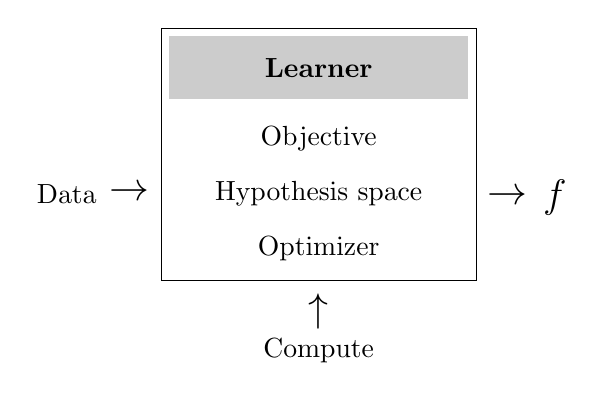
\begin{tikzpicture}
    \draw (0,0) rectangle (4,3.2); % outer box
    \fill[black!20] (0.1,2.3) rectangle (3.9,3.1); % gray box
    \node[] at (2,2.7) {{\bf Learner}};
    \node[] at (2,1.8) {Objective};
    \node[] at (2,1.1) {Hypothesis space};
    \node[] at (2,0.4) {Optimizer};
    \node[] at (-1.2,1.1) {Data};
    \node[] at (-0.4,1.1) {{\Large  $ \rightarrow$}};
    \node[] at (5,1.05) {{\Large $f$}};
    \node[] at (4.4,1.05) {{\Large  $ \rightarrow$}};
    \node[] at (2,-0.4) {{\Large  $ \uparrow$}};
    \node[] at (2,-0.9) {Compute};
\label{fig:ingredients}
\end{tikzpicture}
\end{center}

% \begin{figure}[h]
%     \centering
%     \includegraphics[width=0.5\linewidth]{./figures/intro_to_learning/ingredients.pdf}
%     \label{fig:ingredients}
% \end{figure}

A learner outputs an algorithm, $f: \mathcal{X} \rightarrow \mathcal{Y}$, which maps inputs, $\mathbf{x} \in \mathcal{X}$, to outputs, $\mathbf{y} \in \mathcal{Y}$. Commonly, $f$ is referred to as the \index{Learned function}\textbf{learned function}. The objective that the learner optimizes is typically a function that scores model outputs, $\mathcal{L}: \mathcal{Y} \rightarrow \mathbb{R}$, or compares model outputs to target answers, $\mathcal{L}: \mathcal{Y} \times \mathcal{Y} \rightarrow \mathbb{R}$. We will interchangeably call this $\mathcal{L}$ either the \textbf{objective function}, the \index{Loss function}\textbf{loss function}, or the \textbf{loss}. A loss almost always refers to an objective we seek to \textit{minimize}, whereas an objective function can be used to describe objectives we seek to minimize as well as those we seek to maximize.

\subsection{Importance of Parameterization} The hypothesis space can be described by a set $\mathcal{F}$ of all the possible functions under consideration by the learner. For example, one hypothesis space might be ``all mappings from $\mathbb{R}^2 \rightarrow \mathbb{R}$'' and another could be ``all functions $\mathbb{R} \times \mathbb{R} \rightarrow \mathbb{R}_{\geq 0}$ that satisfy the conditions of being a distance metric.'' Commonly, however, we will not just specify the hypothesis space, but also how we parameterize the space. For example, we may say that our \textit{parameterized} hypothesis space is $y = \theta_1 x + \theta_0$, where $\theta_0$ and $\theta_1$ are the parameters. This example corresponds to the space of affine functions from $\mathbb{R} \rightarrow \mathbb{R}$, but this is not the only way to parameterize that space. Another choice could be $y = \theta_2\theta_1 x + \theta_0$, with parameters $\theta_0$, $\theta_1$, and $\theta_2$. These two choices parameterize \textit{exactly the same space}, that is, any affine functions can be represented by either parameterization and both parameterizations can only represent affine functions. However, these two parameterizations are not equivalent, because optimizers and objectives may treat different parameterizations differently. Because of this, to fully define a learning algorithm, it is important to specify how the hypothesis space is parameterized.\marginnote{\index{Overparameterization}\textbf{Overparameterized} models, where you use more parameters than the minimum necessary to fit the data, are especially important in modern computer vision; most neural networks (\chap{\ref{chapter:neural_nets}}) are overparameterized.}[-3.4cm]
%\marginnote{Recall that a metric function is a very constrained class of functions; metrics must satisfy the triangle inequality, symmetry, nonnegativity, and ``identity of indiscernibles."}
%\marginnote{The role of parameterization can be subtle but should not be overlooked. Historically ... }

\section{Empirical Risk Minimization: A Formalization of Learning from Examples}

The three ingredients from the last section can be formalized using the framework of \index{Empirical risk minimization}{\bf empirical risk minimization} ({\bf ERM}). This framework applies specifically to the supervised setting where we are learning a function that predicts $\mathbf{y}$ from $\mathbf{x}$ given many training examples $\{\mathbf{x}^{(i)},\mathbf{y}^{(i)}\}^N_{i=1}$. The idea is to minimize the average error (i.e., risk) we incur over all the training data (i.e., empirical distribution). The ERM problem is stated as follows:
\begin{align}
    \argmin_{f \in \mathcal{F}} \frac{1}{N} \sum_{i=1}^N \mathcal{L}(f(\mathbf{x}^{(i)}),\mathbf{y}^{(i)}) \quad\triangleleft\quad \text{ERM}
\end{align}
Here, $\mathcal{F}$ is the hypothesis space, $\mathcal{L}$ is the loss function, and $\{\mathbf{x}^{(i)}, \mathbf{y}^{(i)}\}_{i=1}^N$ is the training data (example \{\texttt{input}, \texttt{output}\} pairs), and $f$ is the learned function.

\section{Learning as Probabilistic Inference}
Depending on the loss function, there is often an interpretation of ERM as doing maximum likelihood probabilistic inference. In this interpretation, we are trying to infer the hypothesis $f$ that assigns the highest probability to the data. For a model that predicts $\mathbf{y}$ given $\mathbf{x}$, the max likelihood $f$ is:
\begin{align}
    \argmax_f p\big(\{\mathbf{y}^{(i)}\}_{i=1}^N \given \{\mathbf{x}^{(i)}\}_{i=1}^N, f\big) \quad\quad \triangleleft \quad\text{Max likelihood learning}
\end{align}
The term $p\big(\{\mathbf{y}^{(i)}\}_{i=1}^N \given \{\mathbf{x}^{(i)}\}_{i=1}^N, f\big)$ is called the \index{Likelihood}\textbf{likelihood} of the $\mathbf{y}$ values given the model $f$ and the observed $\mathbf{x}$ values, and maximizing this quantity is called \index{Maximum likelihood learning}\textbf{maximum likelihood learning}.\marginnote{To fully specify this model, we have to define the form of this conditional distribution. One common choice is that the prediction errors, $(\mathbf{y} - f(\mathbf{x}))$, are Gaussian distributed, which leads to the least-squares objective (\sect{\ref{sec:intro_to_learning:least_squares}}).}[-0.4cm]

In later chapters we will see that \textbf{priors} $p(f)$ can also be used for inferring the most probable hypothesis. When a prior is used in conjunction with a likelihood function, we arrive at \index{Maximum a posteriori learning}\textbf{maximum a posteriori learning} (\textbf{MAP learning}), which infers the most probable hypothesis given the training data:
\begin{align}
    &\argmax_f p\big(f \given \{\mathbf{x}^{(i)}, \mathbf{y}^{(i)}\}_{i=1}^N\big) \quad\quad \triangleleft \quad \text{MAP learning}\\
    & = \argmax_f p\big(\{\mathbf{y}^{(i)}\}_{i=1}^N \given \{\mathbf{x}^{(i)}\}_{i=1}^N, f\big)p\big(f\big) \quad\quad \triangleleft \quad \text{by Bayes' rule}
\end{align}


%For example, the least squares regression example we saw above can be interpreted as finding the maximum likelihood estimate of the parameters $\theta$ given the assumption that there truly exists a linear relationship between $x$ and $y$ but that training observations of $y$ are corrupted by Gaussian noise (and we assume that training datapoints are independent and identically distributed, i.e. {\bf iid}).





\section{Case Studies}
The next three sections cover several case studies of particular learning problems. Examples 1 and 3 showcase the two most common workhorses of machine learning: regression and classification. Example 2, Python program induction, demonstrates that the paradigms in this chapter are not limited to simple systems but can actually apply to very general and sophisticated models.

\subsection{Example 1: Linear Least-Squares Regression}\label{sec:intro_to_learning:least_squares}
One of the simplest learning problems is known as \index{Linear least-squares regression}\textbf{linear least-squares regression}. In this setting, we aim to model the relationship between two variables, $x$ and $y$, with a line. 

As a concrete example, let's imagine $x$ represents the temperature outside, and $y$ represents the number people at the beach. As before, we train (i.e., fit) our model on many observed examples of \{\texttt{temperature outside}, \texttt{number of people at the beach}\} pairs, denoted as $\{x^{(i)},y^{(i)}\}_{i=1}^N$. At test time, this model can be applied to predict the $y$ value of a new query $x'$, as shown in \fig{\ref{fig:intro_to_learning:ols_train_test}}.

\begin{figure}[h]
    \centerline{
    \includegraphics[width=0.7\linewidth]{./figures/intro_to_learning/ols_train_test.pdf}
    }
    \caption{The goal of learning is to use the training data to predict the $y$ value of the test query. In our example we find that for every 1 degree increase in temperature, we can expect $\sim 10$ more people to go to the beach.}
    \label{fig:intro_to_learning:ols_train_test}
\end{figure}

Our \emph{hypothesis space} is linear functions, that is, the relationship between $x$ and our predictions $\hat{y}$ of $y$ has the form $\hat{y} = f_{\theta}(x) = \theta_1 x + \theta_0$. This hypothesis space is parameterized by a two scalars, $\theta_0, \theta_1 \in \mathbb{R}$, the intercept and slope of the line. In this book, we will use $\theta$ in general to refer to any parameters that are being learned. In this case we have $\theta = [\theta_0, \theta_1]$. Learning consists of finding the value of these parameters that maximizes the objective.

Our \emph{objective} is that predictions should be near ground truth targets in a least-squares sense, that is, $(\hat{y}^{(i)} - y^{(i)})^2$ should be small for all training examples $\{x^{(i)}, y^{(i)}\}_{i=1}^N$. We call this objective the $L_2$ loss:
\begin{align}
    J(\theta) &= \sum_i \mathcal{L}(\hat{y}^{(i)}, y^{(i)})\\
    &\quad \mathcal{L}(\hat{y}, y) = (\hat{y} - y)^2 \quad\quad \triangleleft \quad L_2 \text{ loss}
\end{align}
\marginnote{We will use $J(\theta)$ to denote the total objective, over all training datapoints, as a function of the parameters; we will use $\mathcal{L}$ to denote the loss per datapoint. That is, $J(\theta) = \sum_{i=1}^N \mathcal{L}(f_{\theta}(x^{(i)}), y^{(i)})$.}[-1.5cm]%Some texts refer to $J$, rather than $\mathcal{L}$, as the ``loss function", but we will reserve the distinct term ``total cost" for $J$ and ``loss" for $\mathcal{L}$.}

%$\mathcal{L}(\hat{y},y) = (\hat{y} - y)^2$ is referred to as the {\bf loss function}, which is defined as the negative of the objective.
%\marginnote{Minimizing the {\bf loss} is equivalent to maximizing the objective.}[-0.0cm]

The full learning problem is as follows:
\begin{align}
    \theta^* = \argmin_{\theta} \sum_{i=1}^N (\theta_1 x^{(i)} + \theta_0 - y^{(i)})^2.
\end{align}
We can choose any number of optimizers to solve this problem. A first idea might be ``try a bunch of random values for $\theta$ and return the one that maximizes the objective.'' In fact, this simple approach works, it just can be rather slow since we are searching for good solutions blind. A better idea can be to exploit \textit{structure} in the search problem. For the linear least-squares problem, the tools of calculus give us clean mathematical structure that makes solving the optimization problem easy, as we show next.

From calculus, we know that at any maxima or minima of a function, $J(\theta)$, with respect to a variable $\theta$, the derivative $\frac{\partial{J(\theta)}}{\partial{\theta}} = 0$. We are trying to find the minimum of the objective $J(\theta)$:
\begin{align}
    J(\theta) = \sum_{i=1}^N (\theta_1 x^{(i)} + \theta_0 - y^{(i)})^2.
\end{align}
This function can be rewritten as
\begin{align}
    J(\theta) = (\mathbf{y} - \mathbf{X}\theta)^\transpose(\mathbf{y} - \mathbf{X}\theta)
\end{align}
with
\begin{align}
\mathbf{X} = 
 \begin{bmatrix}
    1 & x^{(1)}  \\
    1 & x^{(2)} \\
    \vdots & \vdots \\
    1 & x^{(N)}
\end{bmatrix}
\quad
\mathbf{y} = 
 \begin{bmatrix}
    y^{(1)}  \\
    y^{(2)} \\
    \vdots \\
    y^{(N)}
\end{bmatrix}
\quad
\theta = 
 \begin{bmatrix}
    \theta_0 \\
    \theta_1
\end{bmatrix}.
\end{align}

The $J$ is a quadratic form, which has a single global minimum where the derivative is zero, and no other points where the derivative is zero. Therefore, we can solve for the $\theta^*$ that minimizes $J$ by finding the point where the derivative is zero. The derivative is:
\begin{align}
    \frac{\partial J(\theta)}{\partial \theta} =  2(\mathbf{X}^\transpose \mathbf{X} \theta - \mathbf{X}^\transpose \mathbf{y}).
\end{align}
We set this derivative to zero and solve for $\theta^*$:
\begin{align}
    2(\mathbf{X}^\transpose \mathbf{X} \theta^* - \mathbf{X}^\transpose \mathbf{y}) &= 0\\
\mathbf{X}^\transpose \mathbf{X} \theta^* &= \mathbf{X}^\transpose \mathbf{y}\\
\theta^* &= (\mathbf{X}^\transpose\mathbf{X})^{-1}\mathbf{X}^\transpose\mathbf{y}.
\end{align}

The $\theta^*$ defines the best fitting line to our data, and this line can be used to predict the $y$ value of future observations of $x$ (\fig{\ref{fig:intro_to_learning:ols_fit}}).

\begin{figure}[h]
    \centerline{
    \includegraphics[width=1\linewidth]{./figures/intro_to_learning/ols_fit.pdf}
    }
    \caption{A best fit line is a visualization of a function $f_{\theta}$, that predicts the $y$-value for each input $x$-value.}
    \label{fig:intro_to_learning:ols_fit}
\end{figure}

We can now summarize the entire linear least-squares learning problem as follows:

\begin{center}
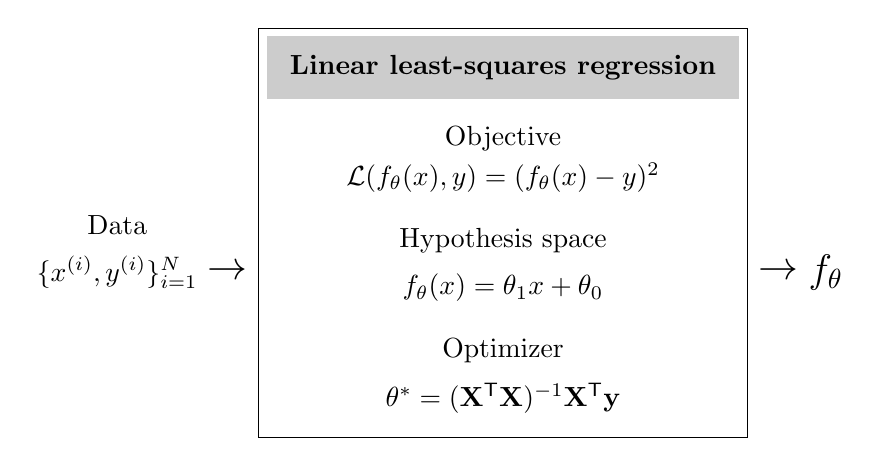
\begin{tikzpicture}
    \draw (0,0) rectangle (6.2,5.2); % outer box
    \fill[black!20] (0.1,4.3) rectangle (6.1,5.1); % gray box
    \node[] at (3.1,4.7) {{\bf Linear least-squares regression}};
    \node[] at (3.1,3.8) {Objective}; \node[] at (3.1,3.3) {$\mathcal{L}(f_{\theta}(x),y) = (f_{\theta}(x)-y)^2$};
    \node[] at (3.1,2.5) {Hypothesis space}; \node[] at (3.1,1.9) {$f_{\theta}(x) = \theta_1 x + \theta_0$};
    \node[] at (3.1,1.1) {Optimizer}; \node[] at (3.1,0.5) {$\theta^* = (\mathbf{X}^\transpose\mathbf{X})^{-1}\mathbf{X}^\transpose\mathbf{y}$};
    \node[] at (-1.8,2.7) {Data};
    \node[] at (-1.8,2.1) {$\{x^{(i)}, y^{(i)}\}_{i=1}^N$};
    \node[] at (-0.4,2.1) {{\Large  $ \rightarrow$}};
    \node[] at (7.2,2.1) {{\Large $f_{\theta}$}};
    \node[] at (6.6,2.1) {{\Large  $ \rightarrow$}};
\label{fig:ols_summary}
\end{tikzpicture}
\end{center}
% \begin{figure}[h]
%     \centering
%     \includegraphics[width=0.6\linewidth]{./figures/intro_to_learning/ols_summary.pdf}
%     \label{fig:ols_summary}
% \end{figure}
\marginnote{In these diagrams, we will sometimes describe the objective just in terms of $\mathcal{L}$, in which case it should be understood that this implies $J(\theta) = \sum_{i=1}^N \mathcal{L}(f_{\theta}(x^{(i)}), y^{(i)})$.}[-4cm]

\subsection{Example 2: Program Induction}
At the other end of the spectrum we have what is known as \index{Program induction}\textbf{program induction}, which is one of the broadest classes of learning algorithm. In this setting, our hypothesis space may be all Python programs. Let's contrast linear least-squares with Python program induction. \Fig{\ref{fig:intro_to_learning:ols_system_diagram}} shows what linear least-squares looks like.

\begin{figure}[h]
    \centerline{
    \includegraphics[width=0.8\linewidth]{./figures/intro_to_learning/ols_system_diagram.pdf}
    }
    \caption{Linear regression finds a line that predicts the training data's $y$-values from its $x$-values.}
    \label{fig:intro_to_learning:ols_system_diagram}
\end{figure}

The learned function is an algebraic expression that maps $x$ to $y$. Learning consisting of searching over two scalar parameters, $\theta_0$ and $\theta_1$.

\Fig{\ref{fig:intro_to_learning:program_induction_system_diagram}} shows Python program induction solving the same problem. In this case, the learned function is a Python program that maps $x$ to $y$. Learning consisted of searching over the space of all possible Python programs (within some max length). Clearly that's a much harder search problem than just finding two scalars. In \chap{\ref{chapter:problem_of_generalization}}, we will see some pitfalls of using too powerful a hypothesis space when a simpler one will do.

\begin{figure}[h]
    \centerline{
    \includegraphics[width=0.8\linewidth]{./figures/intro_to_learning/program_induction_system_diagram.pdf}
    }
    \caption{Python program induction finds a Python program that predicts the training data's $y$-values from its $x$-values.}
    \label{fig:intro_to_learning:program_induction_system_diagram}
\end{figure}

\subsection{Example 3: Classification and Softmax Regression}\label{sec:intro_to_learning:image_classification}

A common problem in computer vision is to recognize objects. This is a \index{Classification}{\bf classification} problem. Our input is an image $\mathbf{x}$, and our target output is a class label $\mathbf{y}$ (\fig{\ref{fig:intro_to_learning:image_classification}}).

\begin{figure}[h]
    \centerline{
    \includegraphics[width=0.7\linewidth]{./figures/intro_to_learning/image_classification.pdf}
    }
    \caption{Image classification.}
    \label{fig:intro_to_learning:image_classification}
\end{figure}

How should we formulate this task as a learning problem? The first question is how do we even represent the input and output? Representing images is pretty straightforward; as we have seen elsewhere in this book, they can be represented as arrays of numbers representing red-green-blue colors: $\mathbf{x} \in \mathbb{R}^{H \times W \times 3}$, where $H$ is image height and $W$ is image width.

How can we represent class labels? It turns out a convenient representation is to let $\mathbf{y}$ be a $K$-dimensional vector, for $K$ possible classes, with $y_k = 1$ if $\mathbf{y}$ represents class $k$, and $y_k = 0$ otherwise. This representation is called a \index{One-hot code}\textbf{one-hot code}, since just one element of the vector is on (``hot''). Each class has a unique one-hot code. We will see why this representation makes sense shortly. The one-hot codes are the targets for the function we are learning. Our goal is to learn a function $f_{\theta}$ that output vectors $\hat{\mathbf{y}}$ that match the one-hot codes, thereby correctly classifying the input images.
%So the learning problem is to map $f_{\theta}: \mathbb{R}^{H \times W \times 3} \rightarrow \mathbb{R}^K$. 
\marginnote{An example of one-hot codes for representing $K$=5 different classes:
\\[6pt]
\centerline{
\includegraphics[width=0.275\linewidth]{figures/intro_to_learning/one_hot_codes_white.eps}
}
}[-1.8cm]

Next, we need to pick a loss function. Our first idea might be that we should minimize misclassifications. That would correspond to the so called \index{0-1 loss}{\bf 0-1 loss}:
\begin{align}
    \mathcal{L}(\hat{\mathbf{y}},\mathbf{y}) = \mathbbm{1}(\hat{\mathbf{y}}\neq\mathbf{y}),
\end{align}
where $\mathbbm{1}$ is the indicator function that evaluates to 1 if and only if its argument is true, and 0 otherwise. Unfortunately, minimizing this loss is a discrete optimization problem, and it is NP-hard. Instead, people commonly use the \index{Cross-entropy loss}{\bf cross-entropy loss}, which is continuous and differentiable (making it easier to optimize):
\begin{align}
    \mathcal{L}(\hat{\mathbf{y}},\mathbf{y}) = H(\mathbf{y}, \hat{\mathbf{y}}) = - \sum_{k=1}^K y_k \log \hat{y}_k \quad\quad \triangleleft \quad \text{cross-entropy loss}
\end{align}
The way to think about this is $\hat{y}_k$ should \textit{represent the probability} we think the image is an image of class $k$. Under that interpretation, minimizing cross-entropy maximizes the log likelihood of the ground truth observation $\mathbf{y}$ under our model's prediction $\hat{\mathbf{y}}$.

For that interpretation to be valid, we require that $\hat{\mathbf{y}}$ represent a \index{Probability mass function}{\bf probability mass function} ({\bf pmf}). A pmf $\mathbf{p}$, over $K$ classes, is defined as a $K$-dimensional vector with elements in the range $[0,1]$ that sums to 1. In other words, $\mathbf{p}$ is a point on the $(K-1)$-\textbf{simplex}, which we denote as \index{Simplex}$\mathbf{p} \in \vartriangle^{K-1}$.\marginnote{The $(K-1)$-simplex, $\vartriangle^{K-1}$, is the set of all $K$-dimensional vectors whose elements sum to 1. $K$-dimensional one-hot codes live on the vertices of $\vartriangle^{K-1}$.}[-1.0cm]

To ensure that the output of our learned function $f_{\theta}$ has this property, i.e., $f_{\theta} \in \vartriangle^{K-1}$, we can compose two steps: (1) first apply a function $z_{\theta}: \mathcal{X} \rightarrow \mathbb{R}^K$, (2) then squash the output into the range $[0,1]$ and normalize it to sum to 1. 
%So, if our parameterized function outputs a vector $f_{\theta}(\mathbf{x}) \in \mathbb{R}^K$, then we can convert it to a pmf by squashing it into the range $[0,1]$ and normalizing it to sum to 1. 
A popular way to squash is via the \index{Softmax}{\bf softmax} function:\marginnote{Using softmax is a modeling choice; we could have used any function that squashes into a valid pmf, that is, a nonnegative vector that sums to 1.}[0.8cm]
\begin{align}
    &\mathbf{z} = z_{\theta}(\mathbf{x})\\
    &\hat{\mathbf{y}} = \texttt{softmax}(\mathbf{z})\\
    &\quad \quad \hat{y}_j = \frac{e^{-z_j}}{\sum_{i=1}^K e^{-z_k}}.
\end{align}
The values in $\mathbf{z}$ are called the \index{Logits}\textbf{logits} and can be interpreted as the unnormalized log probabilities of each class. 
Now we have,
\begin{align}
    \hat{\mathbf{y}} = f_{\theta}(\mathbf{x}) = \texttt{softmax}(z_{\theta}(\mathbf{x}))
\end{align}
\Fig{\ref{fig:softmax_regression_diagram}} shows what the variables look like for processing one photo of a fish during training.

\begin{figure}[h]
    \centering
    \includegraphics[width=1.0\linewidth]{./figures/intro_to_learning/softmax_regression_diagram.pdf}
    \caption{Softmax regression for image classification. The $\odot$ symbol represents an elementwise product. The cross-entropy loss is the negative of the sum over elementwise agreements between the prediction vector $\hat{\mathbf{y}}$ and the label vector $\mathbf{y}$, that is, if $\mathbf{s} = \mathbf{y} \odot \log \hat{\mathbf{y}}$ is the vector of scores for how well our prediction agrees with the label, then our cross-entropy loss is $H(\mathbf{y}, \hat{\mathbf{y}}) = - \sum_{k=1}^K s_k$.}
    \label{fig:softmax_regression_diagram}
\end{figure}

The prediction placed about 40 percent probability on the true class, ``guitarfish,'' so we are 60 percent off from an ideal prediction (indicated by the red bar; an ideal prediction would place 100 percent probability on the true class). Our loss is $-\log 0.4$.

This learning problem, which is also called \index{Softmax regression}{\bf softmax regression}, can be summarized as follows:\marginnote{Softmax regression is just one way to model a classification problem. We could have made other choices for how to map input data to class labels.}[-0.4cm]

\begin{center}
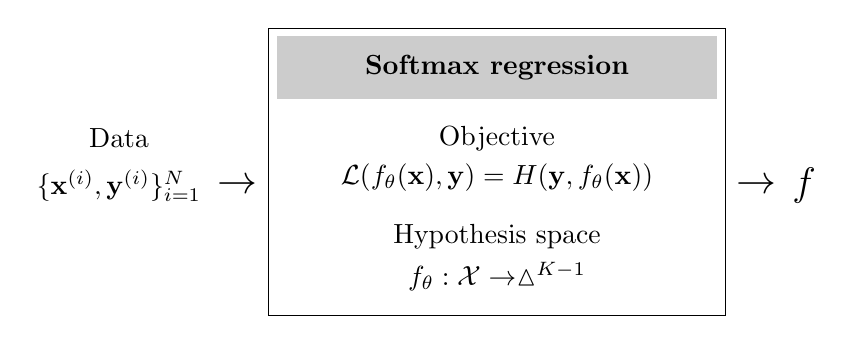
\begin{tikzpicture}
    \draw (0,-1.25) rectangle (5.8,2.4); % outer box
    \fill[black!20] (0.1,1.5) rectangle (5.7,2.3); % gray box
    \node[] at (2.9,1.9) {{\bf Softmax regression}};
    \node[] at (2.9,1.0) {Objective}; \node[] at (2.9,0.5) {$\mathcal{L}(f_{\theta}(\mathbf{x}), \mathbf{y}) = H(\mathbf{y}, f_{\theta}(\mathbf{x}))$};
    \node[] at (2.9,-0.25) {Hypothesis space}; \node[] at (2.9,-0.75) {$f_{\theta}: \mathcal{X} \rightarrow \vartriangle^{K-1}$};
    \node[] at (-1.9,1.0) {Data};
    \node[] at (-1.9,0.4) {$\{\mathbf{x}^{(i)}, \mathbf{y}^{(i)}\}_{i=1}^N$};
    \node[] at (-0.4,0.4) {{\Large  $ \rightarrow$}};
    \node[] at (6.8,0.4) {{\Large $f$}};
    \node[] at (6.2,0.4) {{\Large  $ \rightarrow$}};
\label{fig:softmax_regression_learning_problem}
\end{tikzpicture}
\end{center}
% \begin{figure}[h]
%     \centering
%     \includegraphics[width=0.7\linewidth]{./figures/intro_to_learning/softmax_regression_learning_problem.pdf}
%     \label{fig:softmax_regression_learning_problem}
% \end{figure}
Notice that we have left the hypothesis space only partially specified, and we left the optimizer unspecified. This is because softmax regression refers to the whole family of learning methods that have this general form. This is one of the reasons we conceptualized the learning problem in terms of the three key ingredients described previously: you can often develop them each in isolation, then mix and match.

%\#1 specifies the ``hypothesis space" (aka ``model class") we will search over. A simple model class would be ``linear functions". A more complex model class might be ``C++ programs". \#2 specifies the ``objective function" we wish to optimize. Suppose we are trying to predict tomorrow's weather. Then a natural objective would be that our prediction is close to the truth, for example, we could measure the Euclidean distance between our prediction of the temperature and what its actual value turns out to be. If we use linear functions for our model class, and Euclidean distance for our objective function, then we get what is known as a ``linear least squares" problem. 

%The final question, \#3, is how do we search over the model class to find the instantiation that optimizes the objective? One common approach is hill climbing: starting with some initial parameters, adjust them slightly in the direction that locally improves the objective. Hill climbing can be done by trial and error -- make random adjustments and keep the ones that improved the score -- or by gradient ascent -- use the derivative of the objective function with respect to the parameters to determine the adjustment that will locally increase the objective the most.

%For most of the rest of this class, we will consider machine learning algorithms that answer these three questions as follows:
%\begin{enumerate}
%    \item Hypothesis space: deep neural nets
%    \item Objective: predictions should be close to the truth
%    \item Optimizer: gradient descent
%\end{enumerate}

%What remains is to investigate each of these components in detail.



%\section{Reinforcement learning}
%{\bf Reinforcement learning} is a term that means many different things to different people. A classic definition is learners whose objective is to optimize a {\bf reward function}, rather than to fit a model to examples. A reward function is a mapping from outputs to scores: $r: Y \rightarrow \mathbb{R}$. The learning tries to come up with a function that maximizes rewards.

%However, there is another special distinction of reinforcement learning, and in my opinion a more important distinction: reinforcement learning deals with the setting where data is a function of the learned policy.

%\marginnote{In fact, most terms in machine learning do not have precise, agreed upon definitions. Instead they refer to a collection of connotations, and these connotations will be different in different communities.}[-1.83cm]

%\section{Unsupervised learning}


\section{Learning to Learn}% {\small [Advanced topic]}}

Learning to learn, also called \index{Metalearning}{\bf metalearning}, is a special case of learning where the hypothesis space is learning algorithms. 

Recall that learners train on past instances of a problem to produce an algorithm that can solve future instances of the problem. The goal of metalearning is to handle the case where the future problem we will encounter is itself a learning problem, such as ``find the least-squares line fit to these data points.'' One way to train for this would be by example. Suppose that we are given the following \{\texttt{input}, \texttt{output}\} examples:
\begin{align}
    &\{\texttt{input:} \big(x:[1,2], y:[1,2]\big), &&\texttt{output:} y = x\}\nonumber \\
    &\{\texttt{input:} \big(x:[1,2], y:[2,4]\big), &&\texttt{output:} y = 2x\}\nonumber \\
    &\{\texttt{input:} \big(x:[1,2], y:[0.5,1]\big), &&\texttt{output:} y = \frac{x}{2}\}\nonumber
\end{align}
These are examples of performing least-squares regression; therefore the learner can fit these examples by learning to perform least-squares regression.\marginnote{Note that least-squares regression is not the unique solution that fits these examples, and the metalearner might arrive at a different solution that fits equally well.}[-0.8cm] Since least-squares regression is itself a learning algorithm, we can say that the learner learned to learn.

We started this chapter by saying the learning is a meta-algorithm: it's an algorithm that outputs an algorithm. Metalearning is a meta-meta-algorithm and we can visualize it by just adding another outer loop on top of a learner, as shown in \fig{\ref{fig:intro_to_learning:meta_learning_diagram}}.
\begin{figure}[h]
    \centerline{
    \includegraphics[width=1.0\linewidth]{./figures/intro_to_learning/meta_learning_diagram.pdf}
    }
    \caption{Learning is a meta-algorithm, an algorithm that outputs algorithms; metalearning is just learning applied to learning, and therefore it is a meta-meta-algorithm.}
    \label{fig:intro_to_learning:meta_learning_diagram}
\end{figure}

Notice that you can apply this idea recursively, constructing meta-meta-...-metalearners. Humans perform at least three levels of this process, if not more: we have \emph{evolved} to be \emph{taught} in school how to \emph{learn} quickly on our own.
\marginnote{{\bf Evolution} is a learning algorithm according to our present definition.}[-1.0cm]

\section{Concluding Remarks}
Learning is an extremely general and powerful approach to problem solving. It turns data into algorithms. In this era of big data, learning is very often the preferred approach. It is a a major component of almost all modern computer vision systems.
 % PHILLIP
%\setcounter{chapter}{9}
\chapter{Gradient-Based Learning Algorithms}\label{chapter:gradient_descent}


\section{Introduction}

Once you have specified a learning problem (loss function, hypothesis space, parameterization), the next step is to find the parameters that minimize the loss. This is an optimization problem, and the most common optimization algorithm we will use is \index{Gradient descent}\textbf{gradient descent}. Gradient descent is like a skier making their way down a snowy mountain, where the shape of the mountain is the loss function.

There are many varieties of gradient descent, and we will call this whole family \textbf{gradient-based learning algorithms}. All share the same basic idea: at some operating point, calculate the direction of steepest descent, then use this direction to find a new operating point with lower loss.\marginnote{We use the term \textbf{operating point} to refer to a particular point (setting of the parameters) where we are currently evaluating the loss.}[-0.85cm]

\section{Technical Setting}
In this chapter, we consider the task of minimizing a cost function $J: \cdot \rightarrow \mathbb{R}$, which is a function that maps some arbitrary input to a scalar cost. %The domain of this function can be anything, but the range is always a scalar.

In learning problems, the domain of $J$ is the training data and the parameters $\theta$.\marginnote{Remember from \chap{\ref{chapter:intro_to_learning}} that in supervised learning, the training data is $\{\mathbf{x}^{(i)}, \mathbf{y}^{(i)}\}^N_{i=1}$, while in unsupervised learning the training data is $\{\mathbf{x}^{(i)}\}^N_{i=1}$.} Often, we will consider the training data to be fixed and only denote the objective as a function of the parameters, $J(\theta)$. Our goal is to solve:
\begin{align}
    \theta^* = \argmin_{\theta} J(\theta)
\end{align}

%When we evaluate $J$ at some specific location $\theta$, we will say that is the value of $J$ at operating point $\theta$. 

%$\nabla_{\theta} J \triangleq \frac{\partial J}{\partial \theta}$

Pretty much all optimizers work by some iterative process, where they update the parameters to be better and better. Different optimizers differ in how the parameter update function works. The update function gets to view some information about the loss landscape, then uses that information to update the parameters, as shown in \fig{\ref{fig:gradient_descent:optimization_schematic}}.
\begin{figure}[h]
    \centerline{
    \includegraphics[width=0.35\linewidth]{./figures/gradient_descent/optimization_schematic.pdf}
    }
    \caption{General optimization loop.}
    \label{fig:gradient_descent:optimization_schematic}
\end{figure}

In the simplest setting, called \index{Zeroth-order optimization}\textbf{zeroth-order optimization}, the update function only gets to observe the value $J(\theta)$. The only way, then, to find $\theta$'s that minimize the loss is to sample different values for $\theta$ and move toward the values that are lower.

For gradient-based optimization, also called \index{First-order optimization}\textbf{first-order optimization}, the update function takes as input the gradient of the cost with respect to the parameters at the current operating point, $\nabla_{\theta}J(\theta)$. This reveals hugely useful information about the loss that directly tells us how to minimize it: just move in the direction of steepest descent, that is, the gradient direction.

Higher-order optimization methods observe higher-order derivatives of the loss, such as the Hessian $H$, which tells you how the landscape is locally curving. The Hessian is costly to compute but many methods use approximations to the Hessian, or other properties related to loss curvature, and these are growing in popularity~\cite{martens2015optimizing,foret2020sharpness}.


\section{Basic Gradient Descent}
The simplest version of gradient descent just takes a step in the gradient direction of length proportional to the gradient magnitude. This algorithm is described in \algref{\ref{alg:gradient_descent:basic_gradient_descent}}.
\begin{algorithm}[h]
\SetAlgoVlined
\DontPrintSemicolon
%\marginnote{{\bf Algorithm \ref{alg:gradient_descent:basic_gradient_descent}}: Optimizing a cost function $J: \theta \rightarrow \mathbb{R}$ by descending the gradient $\nabla_{\theta} J$.}
\caption{{\bf Algorithm \ref{alg:gradient_descent:basic_gradient_descent}}: Gradient descent (\texttt{GD}). Optimizing a cost function $J: \theta \rightarrow \mathbb{R}$ by descending the gradient $\nabla_{\theta} J$.}
\fakealgorithmcaption{}
\label{alg:gradient_descent:basic_gradient_descent}
{\bf Input:} objective function $J$, initial parameter vector $\theta^0$, learning rate $\eta$, number of steps $K$\;%, data $\{\mathbf{x}^{(i)},\mathbf{y}^{(i)}\}_{i=1}^N$
{\bf Output:} trained parameter vector $\theta^* = \theta^K$\;
\For{\upshape $k= 0, \dots, K-1$}{
    %$J = \sum_{i=1}^N \mathcal{L}(f_{\theta^{k}}(\mathbf{x}^{(i)}),\mathbf{y}^{(i)})$\;
    $\theta^{k+1} \leftarrow \theta^{k} - \eta \nabla_{\theta} J(\theta^k)$\;
}
\end{algorithm}

This algorithm has two hyperparameters, the \index{Learning rate}\textbf{learning rate} $\eta$, which controls the step size (learning rate times gradient magnitude), and the number of steps $K$. If the learning rate is sufficiently small and the initial parameter vector $\theta^0$ is random, then this algorithm will almost surely converge to a local minimum of $J$ as $K \rightarrow \infty$~\cite{lee2016gradient}. However, to descend more quickly, it can be useful to set the learning rate to a higher value. 

\section{Learning Rate Schedules}
A generally useful strategy is to start with a high value for $\eta$ and then decay it until convergence according to a \textbf{learning rate schedule}. Researchers have come up with innumerable schedules and they generally work by calling some function $\texttt{lr}(\eta^0,k)$ to get the learning rate on each iteration of descent:
\begin{align}
    \eta^{k} = \texttt{lr}(\eta^0,k)
\end{align}
Generally, we want an update rule where $\eta^{k+1} < \eta^k$, so that we take smaller steps as we approach the minimizer. A few simple and popular approaches are given below:
\begin{align}
    \texttt{lr}(\eta^0,k) &= \beta^{-k} \eta^0 &\quad\quad \triangleleft\quad \text{exponential decay}\\
    \texttt{lr}(\eta^0,k) &= \beta^{-\lfloor k/M \rfloor} \eta^0 &\quad\quad \triangleleft\quad \text{stepwise exponential decay}\\
    \texttt{lr}(\eta^0,k) &= \frac{(K - k)}{K} \eta^0 &\quad\quad \triangleleft\quad \text{linear decay}
\end{align}
\marginnote{One downside of linear decay is that it depends on the total number of steps $K$. This makes it hard to compare optimization runs of different lengths. This is something to also be aware of in more advanced learning rate schedules, such as cosine decay~\cite{loshchilov2016sgdr}, which also have different behavior for different settings of $K$.}[-3.2cm]
The $\beta$ and $M$ are additional hyperparameters of these methods. The general approach of learning rate decay is summarized in \algref{\ref{alg:gradient_descent:gradient_descent_with_lr_decay}}.

%but a simple one that tends to work decently is to just multiply the $\eta$ by a  constant factor $\beta \in (0,1)$ every iteration of gradient descent, where $\beta$ and the initial learning rate $\eta^1$ are the new hyperparameters to specify. 
\begin{algorithm}[h]
\SetAlgoVlined
\DontPrintSemicolon
%\marginnote{{\bf Algorithm \ref{alg:gradient_descent:gradient_descent_with_lr_decay}}: Gradient descent with a learning rate schedule.}
\caption{{\bf Algorithm \ref{alg:gradient_descent:gradient_descent_with_lr_decay}}: Gradient descent with a learning rate schedule.}
%\caption{{\bf Algorithm \ref{alg:gradient_descent:gradient_descent_with_lr_decay}}: \texttt{GD}+\texttt{lr}-schedule.}
\fakealgorithmcaption{}
\label{alg:gradient_descent:gradient_descent_with_lr_decay}
{\bf Input:} objective function $J$, initial parameter vector $\theta^0$, initial learning rate $\eta^0$, learning rate function $\texttt{lr}$, number of steps $K$\;%, data $\{\mathbf{x}^{(i)},\mathbf{y}^{(i)}\}_{i=1}^N$
{\bf Output:} trained parameter vector $\theta^* = \theta^K$\;
\For{\upshape $k= 0, \dots, K-1$}{
    %$J = \sum_{i=1}^N \mathcal{L}(f_{\theta^{k-1}}(\mathbf{x}^{(i)}),\mathbf{y}^{(i)})$\;
    $\eta^{k} \leftarrow \texttt{lr}(\eta^0, k)$\;
    $\theta^{k+1} \leftarrow \theta^{k} - \eta^{k} \nabla_{\theta} J(\theta^k)$\;
}
\end{algorithm}

Variations on this algorithm include only decaying the learning rate when a plateau is reached (i.e., when the loss is not decreasing for many iterations in a row), or decaying the learning rate according to more complex nonlinear schedules, such as one shaped like a cosine function~\cite{loshchilov2016sgdr}.%once every $M$ steps of gradient descent, for some fixed value $M$ (which becomes an additional hyperparameter of the algorithm).

\section{Momentum}
Could we do a smarter update than just taking a step in the direction of the gradient? Of the countless ideas that have been proposed, one of the few that has stuck is \index{Momentum}\textbf{momentum}~\cite{polyak1964some,sutskever2013importance}. Momentum makes the analogy to skiing even more precise: momentum is like the inertia of the skier, carrying them over the little bumps and imperfections in the ski slope and increasing their speed as they descend along a straight path. In math, momentum just means that we set the parameter update to be a direction $\mathbf{v}^{k+1}$, given by a weighted combination of the previous update direction, $\mathbf{v}^{k}$, plus the current negative gradient:
\begin{align}
    \mathbf{v}^{k+1} = \mu \mathbf{v}^{k} - \eta\nabla_{\theta} J(\theta^k)
\end{align}
The weight $\mu$ in this combination is a new hyperparameter, sometimes simply called the momentum. The full algorithm is given in \algref{\ref{alg:gradient_descent:gradient_descent_with_momentum}}.
\begin{algorithm}[h]
\SetAlgoVlined
\DontPrintSemicolon
%\marginnote{{\bf Algorithm \ref{alg:gradient_descent:gradient_descent_with_momentum}}: Gradient descent with momentum.}
\caption{{\bf Algorithm \ref{alg:gradient_descent:gradient_descent_with_momentum}}: Gradient descent with momentum.}
\fakealgorithmcaption{}
\label{alg:gradient_descent:gradient_descent_with_momentum}
{\bf Input:} objective function $J$, initial parameter vector $\theta^0$, learning rate $\eta$, momentum $\mu$, number of steps $K$\;%, data $\{\mathbf{x}^{(i)},\mathbf{y}^{(i)}\}_{i=1}^N$
{\bf Output:} trained parameter vector $\theta^* = \theta^K$\;
$\mathbf{v}^{0} = \mathbf{0}$\;
\For{\upshape $k= 0, \dots, K-1$}{
    $\mathbf{v}^{k+1} = \mu \mathbf{v}^{k} - \eta\nabla_{\theta} J(\theta^k)$\;
    $\theta^{k+1} \leftarrow \theta^{k} + \mathbf{v}^{k+1}$\;
}
\end{algorithm}

\Fig{\ref{fig:gradient_descent:momentum_out1}} shows how momentum affects gradient descent for a simple objective $J = \texttt{abs}(\theta)$ (absolute value of $\theta$). As can be seen in the figure, some momentum can help convergence rate (\fig{\ref{fig:gradient_descent:momentum_out1}}, $\mu = 0.5$) but too much momentum will cause the trajectory to overshoot the optimum and even when the optimum loss is achieved, the trajectory might not stop (\fig{\ref{fig:gradient_descent:momentum_out1}}, $\mu = 0.95$).

\begin{figure}[h]
    \centering
    \includegraphics[width=1.0\linewidth]{./figures/gradient_descent/momentum_out1.pdf}
    \caption{(left) A simple loss function $J = \texttt{abs}(\theta)$. (right) Optimization trajectory for three different settings of momentum $\mu$. White line indicates value of the parameter at each iteration of optimization, starting at top and progressing to bottom. Color is value of the loss. Red dot is location where loss first reaches within $0.01$ of optimal value.}
    \label{fig:gradient_descent:momentum_out1}
\end{figure}

It is also possible to come up with other kinds of momentum, which bias the update direction based on some accumulated information from previous updates. Two popular alternatives, which you can read up on elsewhere, are Nesterov's accelerated gradient~\cite{nesterov1983method} and Adam~\cite{kingma2014adam}.


\section{What Kinds of Functions Can Be Minimized with Gradient Descent?}

What if a function is not differentiable? Can we still use gradient descent? Sometimes! The property we need is that we can get a meaningful signal as to how to perturb the function's parameters in order to reduce the loss. This property is \textit{not} the same as differentiability defined in math textbooks. A function may be differentiable but not give useful gradients (e.g., if the gradient is zero everywhere), and a function may be nondifferentiable (at certain points) but still allow for meaningful gradient-based updates (e.g., \texttt{abs}).

\Fig{\ref{fig:gradient_descent:grad_descent_simple_examples}} gives examples of different types of functions being minimized with gradient descent. \Figs{\ref{fig:gradient_descent:grad_descent_simple_examples}}(b) and \ref{fig:gradient_descent:grad_descent_simple_examples}(d) are cases where the function is discontinuous, and the analytical derivative is undefined at the discontinuity. Surprisingly, in \fig{\ref{fig:gradient_descent:grad_descent_simple_examples}}(b), this is not a problem for gradient descent. This is because the gradient descent algorithm we are using here (the one used by Pytorch~\cite{paszke2019pytorch}) uses a \index{One-sided derivative}\textbf{one-sided derivative} at the discontinuity, that is, we set the gradient at the discontinuity to be equal to the gradient value an infinitesimal step away from the discontinuouity in a fixed arbitrary direction. Under the hood, for each atomic discontinuous operation, Pytorch requires that we define its gradients at the discontinuouities, and the one-sided gradient is a standard choice. This is why it can be fine in deep learning (\chap{\ref{chapter:neural_nets}}) to use functions like rectified nonlinear units (relus), which are common in deep networks and have discontinuous gradients.

\Figs{\ref{fig:gradient_descent:grad_descent_simple_examples}}(c) and (e) give cases where the function is continuous, but the gradients are not well-behaved. In \fig{\ref{fig:gradient_descent:grad_descent_simple_examples}}(c) we have a gradient that has nearly \index{Vanishing gradient}\textbf{vanished}, that is, it is near zero everywhere and gradient descent, with a fixed learning rate, will therefore be slow. \Fig{\ref{fig:gradient_descent:grad_descent_simple_examples}}(e) shows the opposite scenario: the gradient at the minimizer goes to infinity; we call this an \index{Exploding gradient}\textbf{exploding gradient}, and this leads to failures of convergence. 

Finally, \fig{\ref{fig:gradient_descent:grad_descent_simple_examples}}(f) shows one more problematic case: when there are multiple minima, gradient descent can get stuck in a suboptimal minimum. Which minimum we arrive at will depend on where we initialized $x$.  

\begin{figure}[h!]
    \centerline{
    \begin{tabular}{cc}
        (a) convex & (b) discontinuous \\
        \includegraphics[width=0.5\linewidth]{./figures/gradient_descent/grad_descent_ex1.pdf} & \includegraphics[width=0.5\linewidth]{./figures/gradient_descent/grad_descent_ex2.pdf} \\
        (c) vanishing gradient & (d) zero gradient + discontinuous \\
        \includegraphics[width=0.5\linewidth]{./figures/gradient_descent/grad_descent_ex4.pdf} &
        \includegraphics[width=0.5\linewidth]{./figures/gradient_descent/grad_descent_ex3.pdf} \\
        (e) exploding gradient & (f) multiple local minima \\
        \includegraphics[width=0.5\linewidth]{./figures/gradient_descent/grad_descent_ex5.pdf} & \includegraphics[width=0.5\linewidth]{./figures/gradient_descent/grad_descent_ex6.pdf}
    \end{tabular}
    }
    \caption{How gradient descent behaves on various functions. In each subplot, left is the function $J$, the red point is the solution found by $\GD$ (with $\eta=0.01$ and $\mu=0.9$), and right is the trajectory of $x$ values over iterations of $\GD$, plotted on top of $J$ at each iteration. (a) As $\eta$ goes to zero, $\GD$ converges for convex functions. (b) Discontinuities pose no essential problem, as long as the gradient is defined on either side. (c) A nearly flat function will exhibit very slow descent. (d) Piecewise constant functions are problematic because the gradient completely vanishes. (e) For the function $J=\texttt{sqrt}(\texttt{abs}(\theta))-0.25$, the gradient goes to infinity at the minimizer, causing instability. (f) When $J$ has multiple local minima, we may not find the global minimum.}
    \label{fig:gradient_descent:grad_descent_simple_examples}
\end{figure}


\subsection{Gradient-Like Optimization for Functions without Good Gradients}\label{sec:gradient_descent:zeroth_order}
What about minimizing functions like \fig{\ref{fig:gradient_descent:grad_descent_simple_examples}}(d), where the gradient is zero almost everywhere? This is a case where gradient descent truly struggles. However, it is often possible to transform such a problem into one that can be treated with gradient descent. Remember that the key property of a gradient, from the perspective of optimization, is that it is a locally loss-minimizing direction in parameter space. Most gradient-based optimizers don't really need true gradients; instead their update functions are compatible with a broader family of local loss-minimizing directions, $\mathbf{v}$. 

Besides the true gradient, what are some other good choices for $\mathbf{v}$? One common idea is to set $\mathbf{v}$ to be the gradient of a \index{Surrogate loss}\textbf{surrogate loss} function, which is a function, $J_{\texttt{surr}}$, with meaningful (non-zero) gradients, that approximates $J$. An example might be a smoothed version of $J$. Another way to get $\mathbf{v}$ is to compute it by sampling perturbations of $\theta$, and seeing which perturbation leads to lower loss. In this strategy, we evaluate $J(\theta+\epsilon)$ for a set of perturbations $\epsilon$, then move toward the $\epsilon$'s that decreased the loss. Approaches of this kind are sometimes called \index{Evolution strategies}\textbf{evolution strategies}~\cite{beyer2002evolution, salimans2017evolution}, and a basic version of this algorithm is given in \algref{\ref{alg:gradient_descent:ES}}.
%\vspace{-0.5cm}
\begin{algorithm}[h!]
\SetAlgoVlined
\DontPrintSemicolon
%\marginnote{{\bf Algorithm \ref{alg:gradient_descent:ES}}: Optimizing a cost function $J: \theta \rightarrow \mathbb{R}$ by evolution strategies, i.e., sampling different values for $\theta$ and taking a step toward the values that work best.}
\caption{{\bf Algorithm \ref{alg:gradient_descent:ES}}: Evolution strategies (\texttt{ES}). Optimizing a cost function $J: \theta \rightarrow \mathbb{R}$ by evolution strategies, i.e., sampling different values for $\theta$ and taking a step toward the values that work best.}
\fakealgorithmcaption{}
\label{alg:gradient_descent:ES}
{\bf Input:} objective function $J$, initial parameter vector $\theta^0$, learning rate $\eta$, sampling standard deviation $\sigma$, number of samples $M$, number of steps $K$\;%, data $\{\mathbf{x}^{(i)},\mathbf{y}^{(i)}\}_{i=1}^N$
{\bf Output:} trained parameter vector $\theta^* = \theta^K$\;
\For{\upshape $k= 0, \dots, K-1$}{
    \For{\upshape $i= 1, \dots, M$}{
        $\epsilon_i \sim \mathcal{N}(\mathbf{0},\mathbf{I})$\;
        $s_i = J(\theta + \sigma \epsilon_i)$\;
    }
    $\theta^{k+1} \leftarrow \theta^{k} - \eta \frac{1}{\sigma M}\sum^M_{i=1} s_i \epsilon_i$\;
}
\end{algorithm}
%\vspace{-0.5cm}

As shown in \fig{\ref{fig:gradient_descent:sampling_out1}}, this algorithm can successfully minimize the function in \fig{\ref{fig:gradient_descent:grad_descent_simple_examples}}(c).
\begin{figure}[h!]
    %\vspace{-0.75cm}
    \centerline{
    \includegraphics[width=0.5\linewidth]{./figures/gradient_descent/sampling_out1.pdf}
    }
    \caption{Using \ES~(\algref{\ref{alg:gradient_descent:ES}}) to minimize a nondifferentiable (zero-gradient) loss, using $\sigma=1$, $M=10$, and $\eta=0.02$.}
    \label{fig:gradient_descent:sampling_out1}
    %\vspace{-0.75cm}
\end{figure}

\subsection{Gradient Clipping}
What about \fig{\ref{fig:gradient_descent:grad_descent_simple_examples}}(e), where the gradient explodes near the optimum? Is there anything we can do to improve optimization of this function? To combat exploding gradients, a useful trick is \index{Gradient clipping}\textbf{gradient clipping}, which just means clamping the magnitude of the gradient to some maximum value. \Algref{\ref{alg:gradient_descent:grad_clipping}} describes this approach.

\begin{algorithm}[h]
\SetAlgoVlined
\DontPrintSemicolon
%\marginnote{{\bf Algorithm \ref{alg:gradient_descent:grad_clipping}}: Gradient descent with gradient clipping.}
\caption{{\bf Algorithm \ref{alg:gradient_descent:grad_clipping}}: Gradient descent with gradient clipping.}
\fakealgorithmcaption{}
\label{alg:gradient_descent:grad_clipping}
{\bf Input:} objective function $J$, initial parameter vector $\theta^0$, learning rate $\eta$, number of steps $K$, max gradient magnitude $m$\;%, data $\{\mathbf{x}^{(i)},\mathbf{y}^{(i)}\}_{i=1}^N$
{\bf Output:} trained parameter vector $\theta^* = \theta^K$\;
\For{\upshape $k= 0, \dots, K-1$}{
    %$J = \sum_{i=1}^N \mathcal{L}(f_{\theta^{k-1}}(\mathbf{x}^{(i)}),\mathbf{y}^{(i)})$\;
    $\mathbf{v} = \nabla_{\theta} J(\theta^k)$\;
    %$\theta^{k+1} \leftarrow \theta^{k} - \eta %[\max(\min(v_1,m),-m),\ldots,\max(\min(v_M,m),-m)]^\transpose$\; %\quad\quad \triangleleft \text{per-dimension clipping}$\;
    %$\theta^{k} \leftarrow \theta^{k-1} - \eta \min(\norm{\mathbf{v}},m)\frac{\mathbf{v}}{\norm{\mathbf{v}}}$\;
     $\theta^{k+1} \leftarrow \theta^{k} - \eta [\texttt{clip}(v_1, -m, m), \ldots, \texttt{clip}(v_M, -m, m)]^\transpose$
}
\end{algorithm}
\marginnote{\texttt{clip} is the ``clipping'' function: $\texttt{clip}(v, -m, m) = \max(\min(v,m),-m)$}[-1.6cm]

This algorithm indeed successfully minimizes our example of the exploding gradient, as can be seen in \fig{\ref{fig:gradient_descent:clipped_out1}}.
\begin{figure}[h]
    \centerline{
    \includegraphics[width=0.5\linewidth]{./figures/gradient_descent/clipped_out1.pdf}
    }
    \caption{Using \GD~with clipping to minimize a loss with exploding gradients, using $m=0.1$.}
    \label{fig:gradient_descent:clipped_out1}
\end{figure}

%This is a case where gradient descent truly struggles. However, with a small modification, gradient descent again becomes applicable. The modification is to descend the gradient of a smooth approximation to $J$, which we will call $J_{\texttt{smooth}}$, rather than to $J$ itself. Given some data, we can either \textit{globally} fit $J_{\texttt{smooth}}$ to $J$, then plug $J_{\texttt{smooth}}$ into Algorithm \ref{alg:gradient_descent:basic_gradient_descent}, or we can proceed in an ``online" fashion, where on each iteration of gradient descent, we \textit{locally} compute: just for this operating point what is the smooth gradient? The latter can be more efficient since we only have to do the approximation for the operating points we visit, which may be a very small subspace of the total parameter space. For this approach, in practice, on each iteration of gradient, we may sample \textbf{finite differences} to find the locally linear approximation to the loss surface:

%The property that we need is that at each operating point, a loss-minimizing direction, $\mathbf{v}$, can given as the input to the update function. This gradient 

% \begin{figure}[h]
%     \centering
%     \includegraphics[width=0.35\linewidth]{./figures/gradient_descent/finite_diffs.pdf}
%     \label{fig:gradient_descent:finite_diffs}
% \end{figure}


%\section{Learning rate schedules}


\section{Stochastic Gradient Descent}\label{sec:gradient_descent:SGD}

One problem with the gradient-based methods we have seen so far is that the gradient may in fact be very expensive to compute, and this is often the case for learning problems. This is because learning problems typically have the form that $J$ is the average of losses incurred on each training datapoint. Computing $\nabla_{\theta}J(\theta)$ requires computing the gradient for each element in the average, that is, the gradient of the function being learned evaluated at the location of each datapoint in the training set. If we train on a big dataset, say 1 million training points, then to perform just \textit{one} step of gradient descent requires computing 1 million gradients! %. If we train on big data, which often we want to do, then even just evaluating $J$, or its gradient, will be expensive.
To make this clear, we will write out $J$ as an explicit function of the training data $\{\mathbf{x}^{(i)}, \mathbf{y}^{(i)}\}_{i=1}^N$. For typical learning problems, $\nabla_{\theta} J(\theta, \{\mathbf{x}^{(i)}, \mathbf{y}^{(i)}\}_{i=1}^N)$ decomposes as follows:
\begin{align}
    \nabla_{\theta} J(\theta, \{\mathbf{x}^{(i)}, \mathbf{y}^{(i)}\}_{i=1}^N) &= %\frac{1}{N}\sum_{i=1}^N \nabla_{\theta} \mathcal{J}(\theta, \mathbf{x}^{(i)}, \mathbf{y}^{(i)})\\
    %&= 
    \nabla_{\theta} \frac{1}{N}\sum_{i=1}^N \mathcal{L}(f_{\theta}(\mathbf{x}^{(i)}), \mathbf{y}^{(i)})\\
    &= \frac{1}{N}\sum_{i=1}^N \nabla_{\theta} \mathcal{L}(f_{\theta}(\mathbf{x}^{(i)}), \mathbf{y}^{(i)})
\end{align}

For large $N$, computing this sum is very expensive. Suppose instead we randomly subsample (without replacement) a \textit{batch} of terms from this sum, $\{\mathbf{x}^{(b)}, \mathbf{y}^{(b)}\}_{b=1}^B$, where $B$ is the \index{Batch size}\textbf{batch size}. We then compute an \textit{estimate} of the total gradient as the average gradient over this batch as follows:
\begin{align}
    \tilde{\mathbf{g}} = \frac{1}{N}\sum_{b=1}^B \nabla_{\theta} \mathcal{L}(f_{\theta}(\mathbf{x}^{(b)}), \mathbf{y}^{(b)})
\end{align}
If we sample a large batch, where $B$ is almost as large as $N$, then the average over the $B$ terms should be roughly the same as the average over all $N$ terms. If we sample a smaller batch, then our estimate of the gradient will be less accurate but faster to compute. Therefore we have a tradeoff between accuracy and speed, and we can navigate this tradeoff with the hyperparameter $B$. The variant of gradient descent that uses this idea is called \index{Stochastic gradient descent}\textbf{stochastic gradient descent} (SGD), because each iteration of descent uses a different randomly (stochastically) sampled batch of training data to estimate the gradient. The full description of \SGD~is given in \algref{\ref{alg:gradient_descent:SGD}}.
\begin{algorithm}[h]
\SetAlgoVlined
\DontPrintSemicolon
%\marginnote{{\bf Algorithm \ref{alg:gradient_descent:SGD}}: Stochastic gradient descent estimates the gradient from a stochastic subset (batch) of the full training data, and makes an update on that basis.}
\caption{{\bf Algorithm \ref{alg:gradient_descent:SGD}}: Stochastic gradient descent (\SGD). Stochastic gradient descent estimates the gradient from a stochastic subset (batch) of the full training data, and makes an update on that basis.}
\fakealgorithmcaption{}
\label{alg:gradient_descent:SGD}
{\bf Input:} initial parameter vector $\theta^{0}$, data $\{\mathbf{x}^{(i)},\mathbf{y}^{(i)}\}_{i=1}^N$, learning rate $\eta$, batch size $B$, number of steps $K$\;
{\bf Output:} trained parameter vector $\theta^* = \theta^K$\;
\For{\upshape $k= 0, \dots, K-1$}{
    $\{\mathbf{x}^{(b)},\mathbf{y}^{(b)}\}_{b=1}^B \sim \{\mathbf{x}^{(i)},\mathbf{y}^{(i)}\}_{i=1}^N \quad\quad \triangleleft \text{ sample batch of training data}$\;
    $\tilde{\mathbf{g}} = \frac{1}{N}\sum_{b=1}^B \nabla_{\theta} \mathcal{L}(f_{\theta}(\mathbf{x}^{(b)}), \mathbf{y}^{(b)})$\;
    $\theta^{k} \leftarrow \theta^{k-1} - \eta \tilde{\mathbf{g}}$\;
}
\end{algorithm}

\SGD~has a number of useful properties beyond just being faster to compute than \GD. Because each step of descent is somewhat random, \SGD~can jump over small bumps in the loss landscape, as long those bumps disappear for some randomly sampled batches. Another important property is that \SGD~can implicitly regularize the learning problem. For example, for linear problems (i.e., $f_\theta$ is linear), then if there are multiple parameter settings that minimize the loss, \SGD~will often converge to the solution with minimum parameter norm~\cite{zhang2021understanding}.

%\section{How to initialize?}

% \section{Parameterization matters}
% \reviewcomment{Unfinished section.}
% \subsection{The power of overparameterization}
% Show a problem where the overparameterized loss landscape has smooth paths of descent (around obstacles) but the less-parameterized loss landscape does not.

\section{Concluding Remarks}
The study of optimization can fill dozens of textbooks and thousands of academic papers. But fortunately for us, modern machine learning has converged on just a few very simple optimization methods that are used in practice. We will soon encounter deep learning, which is the main kind of machine learning used for computer vision. In deep learning, gradient-based optimization is the workhorse. Believe it or not, the handful of algorithms described above are enough to train most state-of-the-art deep learning models. Every year there are new elaborations on these ideas, and second-order methods are ever on the horizon, yet the basic concepts remain quite simple: compute a local estimate of the shape of the loss landscape, then, based on this shape, take a small step toward a lower loss.
%Sometimes this is even treated as definitional to deep learning: deep learning is learning with gradient-based optimization. % PHILLIP
%\setcounter{chapter}{7}

\chapter{The Problem of Generalization}\label{chapter:problem_of_generalization}

\section{Introduction}

So far, we have described learning as an optimization problem: maximize an objective over the \emph{training set}. But this is not our actual goal. Our goal is to maximize the objective over the \emph{test set}. This is the key difference between learning and optimization. We do not have access to the test set, so we use optimization on the training set as a proxy for optimization on the test set. 

Learning theory studies the settings under which optimization on the training set yields good results on the test set. In general it may not, since the test set may have different properties from the training set. When we fit to properties in the training data that do not exist in the test data, we call this {\bf overfitting}. When this happens, training performance will be high, but test performance can be very low, since what we learned about the training data does not {\bf generalize} to the test data.

\section{Underfitting and Overfitting}

A learner may perform poorly for one of two reasons: either it failed to optimize the objective on the training data, or it succeeded on the training data but in a way that does not generalize to the test setting. The former is called \index{Underfitting}{\bf underfitting} and the latter is called \index{Overfitting}{\bf overfitting}.

We will walk through a concrete example of a learner, polynomial regression, that exemplifies these two effects. We introduce this learner briefly in the next subsection before exploring what it tells us about underfitting, overfitting, and generalization.

\subsection{Background: The Polynomial Regression Learning Problem}
Polynomial regression is just like linear regression (\chap{\ref{chapter:intro_to_learning}}) except that the hypothesis space is polynomial functions rather than linear functions, that is,
\begin{align}
y = f_{\theta}(x) = \sum_{k=0}^K \theta_k x^k
\end{align}
where $K$, the degree of the polynomial, is a hyperparameter of the hypothesis space.

Let us consider the setting where we use the least-squares ($L_2$) loss function. It turns out polynomial regression is highly related to linear regression; in fact, we can transform a polynomial regression problem into a linear regression problem! We can see this by rewriting the polynomial as:
\begin{align}
    \sum_{k=0}^K \theta_k x^k = \theta^\transpose\phi(x)\\
    \quad\quad\quad\quad \phi(x) = \begin{bmatrix}
                            1 \\ x \\ x^2 \\ \vdots \\ x^K
                        \end{bmatrix}
\end{align}
Now the form of $f_{\theta}$ is $f_{\theta}(x) = \theta^\transpose\phi(x)$, \textit{which is a linear function in the parameters $\theta$}. Therefore, if we \textit{featurize} $x$, representing each datapoint $x$ with a feature vector $\phi(x)$, then we have arrived at a linear regression problem in this feature space. So, the learning problem, and closed form optimizer, for $L_2$ polynomial regression looks almost identical to that of $L_2$ linear regression:

\begin{center}
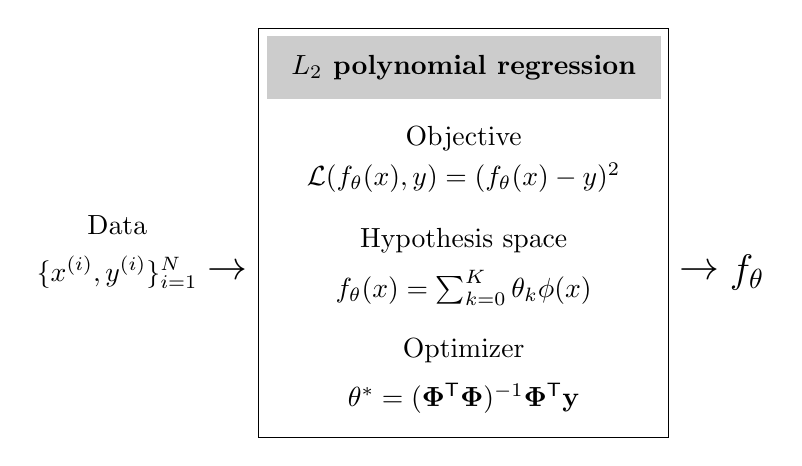
\begin{tikzpicture}
    \draw (0,0) rectangle (5.2,5.2); % outer box
    \fill[black!20] (0.1,4.3) rectangle (5.1,5.1); % gray box
    \node[] at (2.6,4.7) {{\bf $L_2$ polynomial regression}};
    \node[] at (2.6,3.8) {Objective}; \node[] at (2.6,3.3) {$\mathcal{L}(f_{\theta}(x),y) = (f_{\theta}(x)-y)^2$};
    \node[] at (2.6,2.5) {Hypothesis space}; \node[] at (2.6,1.9) {$f_{\theta}(x) = \sum_{k=0}^K \theta_k \phi(x)$};
    \node[] at (2.6,1.1) {Optimizer}; \node[] at (2.6,0.5) {$\theta^* = (\mathbf{\Phi}^\transpose\mathbf{\Phi})^{-1}\mathbf{\Phi}^\transpose\mathbf{y}$};
    \node[] at (-1.8,2.7) {Data};
    \node[] at (-1.8,2.1) {$\{x^{(i)}, y^{(i)}\}_{i=1}^N$};
    \node[] at (-0.4,2.1) {{\Large  $ \rightarrow$}};
    \node[] at (6.2,2.1) {{\Large $f_{\theta}$}};
    \node[] at (5.6,2.1) {{\Large  $ \rightarrow$}};
\end{tikzpicture}
\end{center}

% \begin{figure}[h]
%     \centering
%     \includegraphics[width=0.65\linewidth]{./figures/problem_of_generalization/least_squares_polynomial_regression.pdf}
%     \label{fig:least_squares_polynomial_regression}
% \end{figure}

where
\begin{equation}
    \mathbf{\Phi} = 
     \begin{bmatrix}
        1 & x^{(1)} & x^{(1)^2} & ... & x^{(1)^K} \\
        1 & x^{(2)} & x^{(2)^2} & ... & x^{(2)^K} \\
        \vdots & \vdots & \vdots & \vdots & \vdots \\
        1 & x^{(N)} & x^{(N)^2} & ... & x^{(N)^K}  \\
    \end{bmatrix}
\end{equation}
\marginnote{This same trick works for any kind of function $\phi$, not just polynomials. The $\phi$ could be an expansion into a Fourier basis, for example. The general name for this kind of regression is {\bf basis function regression}; it is equivalent to linear regression on top of \textit{features} of $x$ (i.e., functions of $x$) rather than directly on $x$ itself.}[-6cm]

The matrix $\mathbf{\Phi}$ is an array of the features (columns) for each datapoint (rows). It plays the same role as data matrix $\mathbf{X}$ did in \chap{\ref{chapter:intro_to_learning}}; in fact we often call matrices of the feature representations of each datapoint also as a \textbf{data matrix}. As an exercise, you can derive the closed form of the optimizer, given above, using the same steps as we did for linear regression in \chap{\ref{chapter:intro_to_learning}}.\marginnote{When we get to the chapters on neural nets we will see that data matrices appear all over. A neural net is a sequence of transformations of an input data matrix into increasingly more powerful feature representations of the data, i.e. a sequence of better and better data matrices.}[-4.3cm]

\subsection{Polynomial Regression as a Lens into Generalization}
%To understand underfitting we measure it with {\bf approximation error}. The latter is called overfitting and we measure it with {\bf generalization error}.

What happens as we increase the order of the polynomial $K$, that is, we use $K+1$ basis functions $x^0, \ldots, x^K$? With $K=1$, we arrive back at linear regression. With $K=2$, we are fitting quadratic functions (i.e., parabolas) to the training data. As $K$ increases, the hypothesis space expands to include ever more curvy fits to the data, as shown in \fig{\ref{fig:under_and_overfitting}}.

\begin{figure}[h]
    \centerline{
    \includegraphics[width=1.0\linewidth]{./figures/problem_of_generalization/under_and_overfitting.pdf}
    }
    \caption{Underfitting and overfitting.}
    \label{fig:under_and_overfitting}
\end{figure}

The black line is the model's fit. The green line is the ground truth relationship between random variables $X$ and $Y$. The observed data $\{x^{(i)}, y^{(i)}\}_{i=1}^N$ is the black points, and this data is sampled from the green line plus observation noise. We refer to the full process that generates the data as the {\bf data generating process}:
\begin{align}
    Y &= X^2 + 1 &\triangleleft \quad\text{true underlying relationship}\\
    \epsilon &\sim \mathcal{N}(0,1) &\triangleleft \quad\text{observation noise}\\
    Y^\prime &= Y + \epsilon &\triangleleft \quad\text{noisy observations}\\
    x,y &\sim p(X,Y^{\prime}) &\triangleleft \quad\text{data-generating process}
\end{align}\marginnote{This data generating process assumes there is no noise in our observations of $x$. This is a common assumption in least-squares regression problems. Other models relax this assumption; for example, the generative models we will see in \chap{\ref{chapter:generative_models}} model uncertainty in both the $x$ and $y$ observations jointly.}[-3cm]
As we increase $K$ we fit the data points better and better, but eventually start \emph{overfitting}, where the model perfectly interpolates the data (passes through every datapoint) but deviates more and more from the true data-generating line. Why does that happen? It's because for $K=10$ the curve can become wiggly enough to not just fit the true underlying relationship but also to \textit{fit the noise}, the minor offsets $\epsilon$ around the green line. This noise is \textit{a property of the training data that does not generalize to the test data}; the test data will have different observation noise. That's what we mean when we say a model is overfitting.

As $K$ grows, a second phenomenon also occurs. For $K=10$ there are many hypotheses (polynomial functions) that perfectly the data (true function + noise) -- there is insufficient data for the objective to uniquely identify one of the hypotheses to be the best. Because of this, the hypothesis output by the optimizer may be an arbitrary one, or rather will be due to details of the optimization algorithm (e.g., how it is initialized), rather than selected by the objective. The optimizer we used above has a tendency to pick, among all the equally good hypotheses, one that is very curvy. This is an especially bad choice in this example, because the true function is much more smooth.

%So, overfitting can include two phenomena (both of which we see here): the model can be fitting noise (aspects of training data that don't generalize to test data) and the model might be underconstrained, having no unique minimizer to the objective, and therefore 

\index{Approximation error}{\bf Approximation error} is the gap between the black line and the training data points. Let $\{x_{(\texttt{train})}^{(i)}, y_{(\texttt{train})}^{(i)}\}_{i=1}^N$ be our training data set (the black points). Then the approximation error $J_{\texttt{approx}}$ is defined as the total cost incurred on this training data:
\begin{align}
    J_{\texttt{approx}} = \frac{1}{N} \sum_{i=1}^N \mathcal{L}(f_{\theta}(x_{(\texttt{train})}^{(i)}), y_{(\texttt{train})}^{(i)})
\end{align}
Notice that approximation error is the cost function we minimize in empirical risk minimization (\chap{\ref{chapter:intro_to_learning}}).

\index{Generalization error}{\bf Generalization error} is the gap between the black line and the green line, that is, the expected cost we would incur if we sampled a new test point at random from the true data generating process. Generalization error is often approximated by measuring performance on a heldout \index{Validation dataset}{\bf validation dataset}, $\{x_{(\texttt{val})}^{(i)}, y_{(\texttt{val})}^{(i)}\}_{i=1}^N$, which can simply be a subset of the data that we don't use for training or testing:
\begin{align}
    J_{\texttt{gen}} &= \mathbb{E}_{x,y \sim p_{\texttt{data}}} [ \mathcal{L}(f_{\theta}(x), y)]\\
                        &\approx \frac{1}{N} \sum_{i=1}^N \mathcal{L}(f_{\theta}(x_{(\texttt{val})}^{(i)}), y_{(\texttt{val})}^{(i)})
\end{align}

Approximation error goes down with increasing $K$ but all we really care about is generalization error, which measures how well we will do on test queries that are newly sampled from the true data generating process. For polynomial regression, generalization error obeys a U-shaped function with respect to $K$: at first it is high because we are underfitting; gradually we fit the data better and better and eventually we overfit, with generalization error becoming high again. \Fig{\ref{fig:under_and_overfitting_vs_polyK}} shows how it looks like for our example.
\begin{figure}[h]
    \centerline{
    \includegraphics[width=0.48\linewidth]{./figures/problem_of_generalization/under_and_overfitting_vs_polyK.pdf}
    }
    \caption{Approximation error (\texttt{approx}) versus generalization error (\texttt{gen}) for polynomial regression of order $K$. Here we measured error as the proportion of validation points that are mispredicted (defined as having an $L_2$ prediction error greater than 0.25).}
    \label{fig:under_and_overfitting_vs_polyK}
\end{figure} %We use this notion of error since if we plotted the cost $J_{\texttt{gen}}$ as a function of $K$, for high values of $K$ the error becomes so large that the plot looks like a hockey stick and we only get to see one side of the U-shape.}[2.5cm]

This U-shaped curve is characteristic of classical learning regimes like polynomial regression, where we often find that the more parameters a model has, the more it will tend to overfit. However, this behavior does not well characterize modern learners like deep neural networks. Deep networks, which we will see in \chap{\ref{chapter:neural_nets}}, can indeed either underfit or overfit, but it is not the case that there is a simple relationship between the number of parameters the net has and whether that leads to underfitting versus overfitting. In fact, bigger deep nets with more parameters may overfit less than smaller nets. We discuss this further in \sect{\ref{sect:problem_of_generalization:rethinking_generalization}}. 

%\section{Bias-variance tradeoff}

%This idea can be formalized via the {\bf bias-variance tradeoff}.

%Show empirical plot from DLAICV. 

%An important concept in learning theory is {\bf model capacity}. 


\section{Regularization}

The previous example suggests a kind of ``Goldilocks principle.'' We should prefer hypotheses (functions $f$) that are sufficiently expressive to fit the data, but not so flexible that they can overfit the data. 


\index{Regularization}{\bf Regularization} refers to mechanisms that penalize function complexity so that we avoid learning too flexible a function that overfits. 
%Model capacity measures the expressivity of the hypothesis space. 
Typically, regularizers are terms we add to the objective that prefer simple functions in the hypothesis space, all else being equal. They therefore embody the principle of \index{Occam's razor}{\bf Occam's razor}. The general form of a regularized objective is:
\begin{align}
    J(\theta) = \overbrace{\frac{1}{N} \sum^N_{i=1} \mathcal{L}(f_{\theta}(x)^{(i)}, y^{(i)})}^\text{data fit loss} + \underbrace{\lambda R(\theta)}_\text{regularizer} \quad\quad\triangleleft \quad\text{regularized objective function} \label{eqn:problem_of_generalization:regularized_objective}
\end{align}
where $\lambda$ is a hyperparameter that controls the strength of the regularization.

One of the most common regularizers is to penalize the $L_p$ norm of the parameters of our model, $\theta$:
\begin{equation}
    R(\theta) = \norm{\theta}_{p}.
\end{equation}
\marginnote{The $L_p$-norm of $\mathbf{x}$ is $(\sum_i |x_i|^{p})^{\frac{1}{p}}$. The $L_2$-norm is the familiar least-squares objective.}[-0.4cm]
An especially common choice is $p=2$, in which case the regularizer is called \index{Ridge regression}{\bf ridge regularization} (which is also known as {\bf Tikonov regression}). In the context of neural networks, this regularizer is called \index{Weight decay}{\bf weight decay}. When $p=1$, the regularizer, applied to regression problems, is called \index{LASSO regression}{\bf LASSO regression}. For any $p$, the effect is to encourage most parameters to be zero, or near zero. When most parameters are zero, the function takes on a degenerate form, that is, a simpler form. For example, if we consider the quadratic hypothesis space $\theta_1 x + \theta_2 x^2$, then, if we use a strong $L_p$ regularizer, and if a linear fit is almost perfect, then $\theta_2$ will be forced to zero and the learned function will be linear rather than quadratic. Again, we find that regularization is an embodiment of Occam's razor: when multiple functions can explain the data, give preference to the simplest.

\subsection{Regularizers as Probabilistic Priors} Regularizers can be interpreted as \index{Priors}\textbf{priors} that prefer, a priori (before looking at the data), some solutions over others. Under this interpretation, the data fit loss (e.g., $L_2$ loss) is a likelihood function $p(\{y^{(i)}\}^N_{i=1} \given \{x^{(i)}\}^N_{i=1}, \theta)$ and the regularizer is a prior $p(\theta)$. Bayes' rule then states that the posterior $p(\theta \given \{x^{(i)}, y^{(i)}\}^N_{i=1})$ is proportional to the product of the prior and the likelihood. The log posterior is then the \textit{sum} of the log likelihood and the log prior, plus a constant. Hence we arrive at the form of \eqn{\ref{eqn:problem_of_generalization:regularized_objective}}.

\subsection{Revisiting the $\star$ Problem}\label{sec:problem_of_generalization:star_problem_revisited}
Remember the $\star$ problem from \chap{\ref{chapter:intro_to_learning}}?
\begin{align}
    3 \star 2 &= 36\nonumber \\
    7 \star 1 &= 49\nonumber \\
    5 \star 2 &= 100\nonumber \\
    2 \star 2 &= 16\nonumber
\end{align}
You may have figured out that $x \star y = (xy)^2$. We said that is the correct answer. But hold on, couldn't it be that $x \star y =  94.5x - 9.5x^2 + 4y^2 - 151$? That also perfectly explains these four examples (trust us, we checked). Or maybe $\star$ is the following Python program (\fig{\ref{fig:problem_of_generalization:python_star_solution}}).
\begin{figure}[h]
\begin{minipage}{1.0\linewidth}
\begin{minted}[xleftmargin=0.33\linewidth,xrightmargin=0.33\linewidth,
fontsize=\fontsize{8.5}{9},
frame=single,
framesep=2.5pt,
baselinestretch=1.05,
]{python}
def star(x,y):
    if x==2 && y==3:
        return 36
    elif x==7 && y==1:
        return 49
    elif x==5 && y==2:
        return 100
    elif x==2 && y==2:
        return 16
    else:
        return 0
\end{minted}
\end{minipage}
%}
\caption{A function written in Python that solves the $\star$ problem from \chap{\ref{chapter:intro_to_learning}}.}
\label{fig:problem_of_generalization:python_star_solution}
\end{figure}

That also perfectly fits the observed data. Why didn't you come up with those answers? What made $x \star y = (xy)^2$ more compelling?

We suspect your reason is again Occam's razor, which states that when multiple hypotheses equally well fit the data, you should prefer the simplest. To a human, it may be that $x \star y = (xy)^2$ is the simplest. To a computer, defining a proper notion of simplicity is a hard problem, but can be made precise.

As we saw, most regularizers can be given probabilistic interpretations as priors on the hypothesis, whereas the original objective (e.g., least-squares) measures the likelihood of the data given the hypothesis. These priors are not arbitrarily chosen. The notion of the {\bf Bayesian Occam's razor} derives such priors by noting that more complex hypothesis spaces must cover more possible hypotheses, and therefore must assign less prior mass to any single hypothesis (the prior probability of all possible hypotheses in the hypothesis space must sum to 1)~\cite{jefferys1992ockham, mackay2003information}. This is why, probabilistically, simpler hypotheses are more likely to be true.

\section{Rethinking Generalization} \label{sect:problem_of_generalization:rethinking_generalization}
A recent empirical finding is that some seemingly complex hypothesis spaces, such as deep nets (which we will see in later chapters), tend not to overfit, even though they have many more free parameters than the number of datapoints they are fit to. Exactly why this happens is an ongoing topic of research~\cite{zhang2016understanding}. But we should not be too surprised. The number of parameters is just a rough proxy for model capacity (i.e., the expressivity of the hypothesis space). A single parameter that has infinite numerical precision can parameterize an arbitrarily complex function. Such a parameter defines a very expressive hypothesis space and will be capable of overfitting data. Conversely, if we have a million parameters, but they are regularized so that almost all are zero, then these parameters may end up defining a simple class of functions, which does not overfit the data. So you can think of the number of parameters as a rough estimate of model capacity, but it is not at all the full story. See \cite{belkin2018reconciling} for more discussion on this point.%Overfitting is fundamentally related to \emph{model capacity}, not number of parameters, but often number of parameters is a good proxy. %Ideas from information theory can be used to define more appropriate measures of expressivity than ``number of parameters". %However, it has long been clear that overfitting is not really about \emph{number} of free parameters, rather the complexity of the hypothesis space. A function with many parameters tends to be more complex than a function with   

\section{Three Tools in the Search for Truth: Data, Priors, and Hypotheses}

In this section, we will introduce a perspective on learning and generalization that puts all our tools together. We will consider learning as akin to searching for the proverbial needle in a haystack. The haystack is our search space (i.e., the hypothesis space). The needle is the ``truth'' we are seeking, that is, the true function that generates our observations. 

We have several tools at our disposal to help us pinpoint the location of the needle, and in this section we will focus on the following three: \textit{data}, \textit{priors}, and \textit{hypotheses}. 

The first tool, \textit{data}, was the topic of \chap{\ref{chapter:intro_to_learning}}. In vision, the data is observations of the world like photos and videos. Finding explanations consistent with the observed data is the centerpiece of learning-based vision.

The second tool at our disposal was introduced earlier in this chapter: priors (a.k.a. regularizers) that prefer some solutions over others a priori. 

The last tool at our disposal is the set of \textit{hypotheses} under consideration for what the true function may be. The hypothesis space constrains which solutions we can possibly find. If the true solution is not in our hypothesis space, then no amount of data or priors can help us find it. This situation is like the old joke of a drunk man looking for his lost keys under a lamppost~\cite{freedman2010wrong}. ``Why are you looking there,'' a cop asks. ``Because this is where the light is.''

Together these three tools allow us to pinpoint one (or a few) good solutions in the space of all possibilities, as depicted in the cartoon in \fig{\ref{fig:problem_of_generalization:search_space_tools}}.
%\vspace{-0.3cm}

In this cartoon, we are learning a mapping from some domain $\mathcal{X}$ to another domain $\mathcal{Y}$. The hypothesis space, $\mathcal{F}$ (white circle; ``the lamppost's light'') places a hard constraint on the subset of possible mappings under consideration, the prior (yellow ellipse) places a soft constraint on which mappings are preferred over which others, and the data (green ellipse) also places a soft constraint on the space, preferring mappings that well fit the data. 

\begin{figure}[t]
    \centerline{
    \includegraphics[width=0.65\linewidth]{./figures/problem_of_generalization/search_space_tools.pdf}
    }
    \caption{A cartoon of the tools for honing in on the truth.}
    \label{fig:problem_of_generalization:search_space_tools}
\end{figure}


Approximation error is low within the green region. If we didn't care about generalization, then it would be sufficient just to select any solution in this green region. But since we do care about generalization, we bias our picks toward the yellow region, which corresponds to a prior that selects points we believe to be closer to the true solution, even if they might not fit the data perfectly well. These tools isolate the area outlined in bright yellow as the region where we may find our needle of truth. A learning algorithm, which searches over $\mathcal{F}$ in order to maximize the likelihood times the prior, will find a solution somewhere in this outlined region. %The found solution will not necessarily coincide with the true solution but cannot be too far off, as long as the yellow outlined region indeed contains the truth. %will hopefully be nearby; if we shrink the yellow outlined region then we can be force the learner to get ever closer to the truth. 
%But it might not find the exact location of the true solution as the intersection of all our tools did not identify a unique solution in this example.

In the next three sections, we will explore these three tools in more detail through the simple experiment of fitting a curve to a set of datapoints.


\subsection{Experiment 1: Effect of Data}

Training data is the main source of information for a learner, and a learner is just like a detective: as it observes more and more data, it gets more and more evidence to narrow in on the solution. Here we will look at how data shapes the objective function $J$ for the following empirical risk minimization problem:
\begin{align}
    J(\theta; \{x^{(i)}, y^{(i)}\}^N_{i=1}) &= \frac{1}{N}\sum_i \lvert f_{\theta}(x^{(i)}) - y^{(i)}\rvert^{0.25} \quad\quad \triangleleft \quad\text{objective}\label{eqn:problem_of_generalization:error_fn_1}\\
    f_{\theta}(x) &= \theta_0 x + \theta_1 \sin(x)  \quad\quad \triangleleft \quad\text{hypothesis space}
\end{align}\marginnote{We use the exponent $0.25$, rather than the more common squared error, just so that the plots in \fig{\ref{fig:problem_of_generalization:more_data_more_constraints}} show more clearly the linear constraints (the dark lines) added by each datapoint to the objective $J$.}[-1.6cm]
In \fig{\ref{fig:problem_of_generalization:more_data_more_constraints}}, bottom row, we plot $J$ as a heatmap over the values obtained for different settings of $\theta$. On the top row we plot the data being fit, $\{x^{(i)}, y^{(i)}\}^N_{i=1}$, along with the function $f_{\theta}$ that achieves the best fit, and a sample other settings of $\theta$ that achieve within 0.1 of the cost of the best fit. Each column corresponds to some amount of training data $N$. Moving to the right, we increase $N$.

\begin{figure}[t]
    \centerline{
    \includegraphics[width=1.0\linewidth]{./figures/problem_of_generalization/more_data_more_constraints.pdf}
    }
    \caption{More data, more (soft) constraints.}
    \label{fig:problem_of_generalization:more_data_more_constraints}
\end{figure}
\marginnote{The heatmaps here are reminiscent of a classic computer vision algorithm called the Hough transform~\cite{hough1959machine,duda1972use}. This transform can be used to find geometric primitives that fit feature points in images. In fact, the bottom row is \textit{exactly} the generalized Hough transform~\cite{duda1972use} of the data points in the top row, using $\theta_0 x + \theta_1 \sin(x)$ as the family of geometric primitives we are fitting.}[-9cm]

The first thing to look at is the leftmost column, where $N=1$. For a single datapoint, there are an infinite number of functions in our hypothesis space that perfectly fit that point. This shows up in the heatmaps as a \textit{line} of settings of $\theta$ that all achieve zero loss.\marginnote{Why a line? Because we have \textit{two} free parameters, $[\theta_0, \theta_1]$, and \textit{one} constraint, $y^{(1)} = \theta_0 x^{(1)} + \theta_1 \sin(x^{(1)})$, so we have one more parameter than constraint yielding a one-dimensional (1D) subspace of solutions.}[-0.4cm] The learning algorithm we used in this example picks a random solution from the set of solutions that achieve zero loss. Unfortunately, here it got unlucky and picked a solution that happens to be far from the true solution.

Next, look at the second column where we have $N=5$ training points. Ideally we want to find a curve that exactly passes through each point. Each \textit{single} datapoint adds one constraint to this problem, and each constraint shows up as a line in the heatmap for $J$ [the line of solutions that satisfy the constraint $y^{(i)} = \theta_0 x^{(i)} + \theta_1 \sin(x^{(i)})$ for that datapoint $i$]. The \textit{intersection} of all these constraints pinpoints the setting of parameters that fits \textit{all} that data. In this example, with five datapoints, there is no location where all the constraint lines intersect, which means there is no curve in our hypothesis space that can perfectly fit this data. Instead we settle for the curve that best approximates the data, according to our loss function. Notice that the learned solution is now pretty close to the true function that generated the data. It is not an exact match, because the data is generated by taking \textit{noisy} samples from the true data generating function.

Finally, let's look at the third column, where we are fitting 20 datapoints. Now the intersection (or, more precisely, average) of the losses for all the datapoints gives a relatively smooth cost function $J(\theta)$, and the learned solution is almost right on top of the true solution. This illustrates a very important point:
\begin{center}
    \textit{The more data you have, the less you need other modeling tools.}
\end{center}%\marginnote{As long as 1) the truth is within the hypothesis space, 2) the noise level is finite, and 3) what you care about is inferring truth.}

With enough data, the true solution will be pinpointed by data alone. However, when we don't have enough data, or when the data is noisy or incorrectly labeled, we can turn to our two other tools, which we will see next.
% processing is too expensive

%This point has several implications that are good to keep in mind. First, generally, the more data you have the better. Second, the more data you have, the less you need other tools to identify the truth -- if you have enough data you don't need regularizers or constraints. Third, because data scale tends to increase over time (we have more and can process more), you should expect that whatever architecture/regularizers are used in year $X$, a less constrained architecture with less regularized will be preferred in year $Y$, for $Y>X$. This is a rule of thumb that has been borne time and again: whatever \textit{inference} methods you learn in this book (meaning optimizers, features, objectives, architectures, models, etc), expect that fewer and fewer of them will be relevant in each subsequent year. Not because new methods will come along that make the current ones out of date (yes that will happen too) but because fewer and fewer methods are useful as data and compute scale. In some year $Z$ we will have enough data and compute that very ``naive'' methods are just as effective as the most sophisticated present approaches. This idea has been called ``the bitter lesson'' and it's good to get comfortable with it now so that you won't have a bitter surprise in a few years. 


\subsection{Experiment 2: Effect of Priors}

Now we will run a similar experiment to look at the effect of priors. In this experiment we will use a slightly different hypothesis space and objective function, namely
\begin{align}
    J(\theta; \{x^{(i)}, y^{(i)}\}^N_{i=1}) &= \frac{1}{N}\sum_i \norm{f_{\theta}(x^{(i)}) - y^{(i)}}_2^2 + \lambda \norm{\theta}_2^2 \quad\quad \triangleleft \quad\text{objective}\\
    f_{\theta}(x) &= \theta_0 x + \theta_1 x \quad\quad \triangleleft \quad\text{hypothesis space}
\end{align}
We will look at the effect of the ridge regularizer $\norm{\theta}_2^2$. We plot the energy landscape and function fit for this problem in \fig{\ref{fig:problem_of_generalization:more_regularizer_more_constraints}}, fitting to a single datapoint. The ridge regularizer prefers solutions with small parameter norm, so its contribution to the energy landscape is to place a quadratic bowl around the origin. As we increase $\lambda$ (moving left to right in the subplots), the effect of the regularizer becomes stronger and pulls the learned solution closer and closer to the origin.

\begin{figure}[t]
    \centerline{
    \includegraphics[width=1.0\linewidth]{./figures/problem_of_generalization/more_regularizer_more_constraints.pdf}
    }
    \caption{More regularization, more (soft) constraints.}
    \label{fig:problem_of_generalization:more_regularizer_more_constraints}
\end{figure}

In this example, the true solution lies near the origin, so adding some regularization gets us closer to the truth. But using too strong a $\lambda$ overregularizers; the true solution is not \textit{exactly} $\theta=0$. The middle column is the Goldilocks solution, where the strength of the regularizer is just right.

You can take away a few lessons from this example:
\begin{enumerate}
    \item Priors help only when they are good guesses as to the truth.
    \item Overreliance on the prior means ignoring the data, and this is generally a bad thing.
    \item For any given prior, there is a sweet spot where the strength is optimal. Sometimes this ideal strength can be derived from modeling assumptions and other times you may need to tune it as a hyperparameter.
\end{enumerate}

\subsection{Experiment 3: Effect of the Hypothesis Space}

Now we turn to the last of our tools: the hypothesis space itself. For this experiment, we will use the same objective as in \eqn{\ref{eqn:problem_of_generalization:error_fn_1}} and we will consider the following three hypothesis spaces:
\begin{align}
    f_{\theta}(x) &= \theta_0 x + \theta_1 x^2 &\triangleleft \quad\texttt{quadratic}\\
    f_{\theta}(x) &= \theta_0 x &\triangleleft \quad\texttt{linear}\\
    f_{\theta}(x) &= 0 &\triangleleft \quad\texttt{constant}
\end{align}
Our experiment on these three spaces is shown in \fig{\ref{fig:problem_of_generalization:fewer_hypotheses_more_constraints}}. We show the hypothesis spaces in order of decreasing size moving to the right.

\begin{figure}[t]
    \centerline{
    \includegraphics[width=1.0\linewidth]{./figures/problem_of_generalization/fewer_hypotheses_more_constraints.pdf}
    }
    \caption{Fewer hypotheses, more (hard) constraints.}
    \label{fig:problem_of_generalization:fewer_hypotheses_more_constraints}
\end{figure}

The true function is linear, and because of that both the \texttt{quadratic} and \texttt{linear} hypothesis spaces contain the true solution. However, the linear hypothesis space is \textit{much} smaller than the quadratic space. For the linear hypothesis space, searching for the solution (i.e., learning) only considers the slice of parameter space where $\theta_1=0$; all the gray region in \fig{\ref{fig:problem_of_generalization:fewer_hypotheses_more_constraints}} can be ignored. Using a smaller hypothesis space can potentially accelerate our search. %This leads us to a general principle:
%\begin{center}
%    \textit{A smaller hypothesis space can accelerate the search for truth.}
%\end{center}
%\marginnote{Remember, the hypothesis space and parameterization are \textit{not} the same thing (see \chap{\ref{chapter:intro_to_learning}}, \sect{\ref{sec:intro_to_learning:key_ingredients}}). \textit{Overparameterizating} a small hypothesis space can make learning faster.}[-0.4cm]

However, clearly you can go too far, as is demonstrated by the \texttt{constant} hypothesis space (far right column). This hypothesis space only contains one function, namely $f_{\theta}(x) = 0$. Search is trivial, but the truth is not in this space.

%One important thing to note is that the hypothesis space is not the same as the parameterization. The same hypothesis space can be parameterized in many ways. For example, a linear function $\mathbb{R} \rightarrow \mathbb{R}$ can be parameterized either as $f_{\theta}(x) = \theta_0 x$ or as $f_{\theta}(x) = \theta_1 \theta_0 x$, or as $f_{\theta}(x) = (\theta_1 + \theta_0) x$ or infinite other possiblities, as long as the parameters all end up describing a linear function of $x$. All these parameterizations span the same hypothesis space: linear relationships between $x$ and $y$. You might be tempted to think that fewer parameters is better, since a smaller hypothesis space is generally better (as long as it contains the truth). But this is not always the case. \textit{Overparameterized} models, which have more parameters than the minimum necessary to describe the hypothesis space, sometimes confer benefits in terms of implicit regularization and optimization speed~\cite{XX}. The virtues of overparameterization are being actively studied in the context of deep neural nets (which are generally highly overparameterized)~\cite{XX}.

\subsection{Summary of the Experiments}

These three experiments demonstrate that data, priors, and hypotheses can all constrain our search in similar ways. All three rule out some parts of the full space of mappings and help us focus on others. 

This leads us to another general principle:
\begin{center}
    \textit{What can be achieved with any one of our tools can also be achieved with any other.\footnote{However, note that the hypothesis space places \textit{hard} constraints on our search; we cannot violate them. Data and priors apply \textit{soft} constraints; we can violate them but we will pay a penalty.}}
\end{center}
%\marginnote{* However, note that the hypothesis space places \textit{hard} constraints on our search; we cannot violate them. Data and priors apply \textit{soft} constraints; we can violate them but we will pay a penalty.}
If you don't have much data, you can use strong priors and structural constraints instead. If you don't have much domain knowledge, you can collect lots of data instead. This principle was nicely articulated by Ilya Sutskever when he wrote that ``methods ... are extra training data in disguise''~\cite{dataindisguise}. %And we can equally well say: training data is extra methods in disguise.


\section{Concluding Remarks}
The goal of learning is to extract lessons from past data to help on future problem solving. Unless the future is \textit{identical} to the past, this is a problem that requires generalization. One goal of learning algorithms is to make systems that generalize ever better, meaning they continue to work even when the test data is very different than the training data. Currently, however, the systems that generalize in the strongest sense—that work \textit{for all} possible test data—are generally not learned but designed according to other principles. In this way, many classical algorithms still have advantages over the latest learned systems. But this gap is rapidly closing! % PHILLIP

\chapter{Neural Networks}\label{chapter:neural_nets}
%\textit{Draft chapter from Torralba, Isola, Freeman}

\section{Introduction}
Neural networks are functions loosely modeled on the brain. In the brain, we have billions of neurons that connect to one another. Each neuron can be thought of as a node in a graph, and the edges are the connections from one neuron to the next (\fig{\ref{fig:neural_nets:fig1_net}}). The edges are directed; electrical signals propagate in just one direction along the wires in the brain.

\begin{figure}[h]
\centerline{
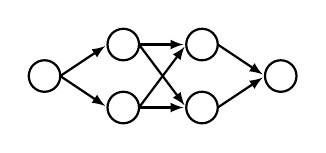
\begin{tikzpicture}%[>=spaced latex]
\draw [thick] (0,0) circle [radius=0.2];
\draw [thick] [nn_edge] (0.2,0) -- (0.8,-0.4);
\draw [thick] [nn_edge] (0.2,0) -- (0.8,0.4);
\draw [thick] (1,-0.4) circle [radius=0.2];
\draw [thick] (1,0.4) circle [radius=0.2];
\draw [thick] [nn_edge] (1.2,-0.4) -- (1.8,-0.4);
\draw [thick] [nn_edge] (1.2,0.4) -- (1.8,0.4);
\draw [thick] [nn_edge] (1.2,-0.4) -- (1.8,0.4);
\draw [thick] [nn_edge] (1.2,0.4) -- (1.8,-0.4);
\draw [thick] (2,-0.4) circle [radius=0.2];
\draw [thick] (2,0.4) circle [radius=0.2];
\draw [thick] [nn_edge] (2.2,-0.4) -- (2.8,0);
\draw [thick] [nn_edge] (2.2,0.4) -- (2.8,0);
\draw [thick] (3.0,0) circle [radius=0.2];
\end{tikzpicture}
}
\caption{A neural network can be drawn as a directed graph.}
\label{fig:neural_nets:fig1_net}
\end{figure}


Outgoing edges are called axons and incoming edges are called dendrites. A neuron fires, sending a pulse down its axon, when the incoming pulses, from the dendrites, exceed a threshold. 

\section{The Perceptron: A Simple Model of a Single Neuron}
Let's consider a neuron, shaded in gray, that has four inputs and one output (\fig{\ref{fig:neural_nets:perceptron_fig2}}).
\begin{figure}[h]
\centerline{
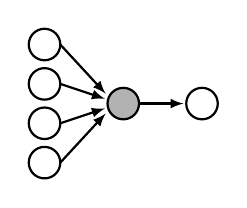
\begin{tikzpicture}[>=spaced latex]
\draw [thick] (0,-0.75) circle [radius=0.2];
\draw [thick] (0,-0.25) circle [radius=0.2];
\draw [thick] (0,0.25) circle [radius=0.2];
\draw [thick] (0,0.75) circle [radius=0.2];
\draw [thick] [nn_edge] (0.2,-0.75) -- (0.8,-0.1);
\draw [thick] [nn_edge] (0.2,-0.25) -- (0.8,-0.05);
\draw [thick] [nn_edge] (0.2,0.25) -- (0.8,0.05);
\draw [thick] [nn_edge] (0.2,0.75) -- (0.8,0.1);
\draw [thick, fill=gray_neuron] (1,0) circle [radius=0.2];
\draw [thick] [nn_edge] (1.2,0) -- (1.8,0);
\draw [thick] (2.0,0) circle [radius=0.2];
\end{tikzpicture}
}
\caption{Perceptron.}
\label{fig:neural_nets:perceptron_fig2}
\end{figure}

A simple model for this neuron is the \index{Perceptron}{\bf perceptron}. A perceptron is a neuron with $n$ inputs $\{x_i\}_{i=1}^n$ and one output $y$, that maps inputs to outputs according to the following equations:
\begin{align}
    z = f(\mathbf{x}) &= \sum_{i=1}^n w_i x_i + b = \mathbf{w}^\transpose\mathbf{x} + b &\triangleleft \quad \text{linear layer}\\
    g(z) &= \begin{cases}
    1, &\text{if} \quad z > 0\\
    0,              & \text{otherwise}
\end{cases} &\triangleleft \quad \text{activation function}\label{eqn:neural_nets:perceptron_activation}\\
    y &= g(f(\mathbf{x})) &\triangleleft \quad \text{perceptron}
\end{align}

In words, we take a weighted sum of the inputs and, if that sum exceeds a threshold (here 0), the neuron fires (outputs a 1). The function $f$ is called a \index{Linear layer}{\bf linear layer} because it computes a linear function of the inputs, $\mathbf{w}^\transpose\mathbf{x}$, plus a \index{Bias}\textbf{bias}, b. The function $g$ is called the \index{Activation function}{\bf activation function} because it decides whether the neuron activates (fires).\marginnote{Mathematically, $f$ is an affine function, but by convention we call it a ``linear layer.'' One way to think of it is $f$ is a linear function of $\begin{bmatrix}\mathbf{x}\\ 1\end{bmatrix}$.}[-0.8cm]

\subsection{The Perceptron as a Classifier}
People got excited about perceptrons in the late 1950s because it was shown that they can learn to classify data~\cite{rosenblatt1958perceptron}. Let's see how that works. We will consider a perceptron with two inputs, $x_1$ and $x_2$, and one output, $y$. Let the incoming connection weights be $w_1 = 2$, $w_2 = 1$, and $b=0$. The values of $z$ and $y$, as a function of $x_1$ and $x_2$, are shown in \fig{\ref{fig:neural_nets:perceptron_as_classifier}}.

\begin{figure}[h]
\centerline{

\noindent\hspace{0.05\linewidth}
\begin{minipage}{.25\linewidth}

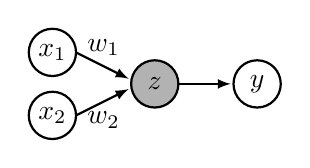
\begin{tikzpicture}[>=spaced latex]
\draw [thick] (0,-0.4) circle [radius=0.3] node {$x_2$};
\draw [thick] (0,0.4) circle [radius=0.3] node {$x_1$};
\draw [thick] [nn_edge] (0.3,-0.4) -- (1.0,-0.05) node[midway,below] {$w_2$};
\draw [thick] [nn_edge] (0.3,0.4) -- (1.0,0.05) node[midway,above] {$w_1$};
\draw [thick, fill=gray_neuron] (1.3,0) circle [radius=0.3] node {$z$};
\draw [thick] [nn_edge] (1.6,0) -- (2.3,0);
\draw [thick] (2.6,0) circle [radius=0.3] node {$y$};
\end{tikzpicture}

\end{minipage}
\begin{minipage}{.68\linewidth}

\begin{tikzpicture}
\begin{axis}[name=plot1, view={0}{90}, xmin=-1, xmax=1, ymin=-1, ymax=1, 
width=0.5\linewidth, xlabel=$x_1$, ylabel=$x_2$, 
title=$z$,
axis equal image,
x label style={at={(axis description cs:0.5,-0.17)}},
y label style={at={(axis description cs:-0.17,0.5)}},
]
	\addplot3[surf, shader=interp, domain=-1:1] {2*x+y};
	\end{axis}
%\end{tikzpicture}
%\end{minipage}
%\begin{minipage}{.30\linewidth}
%\begin{tikzpicture}
\begin{axis}[name=plot2, at=(plot1.right of south east), xshift=30, view={0}{90}, xmin=-1, xmax=1, ymin=-1, ymax=1, 
width=0.5\linewidth, xlabel=$x_1$, ylabel=$x_2$,
title=$y$,
colorbar,
colorbar style={
        ytick={-3.0,-2.0,-1.0,0,1.0,2.0,3.0},
        yticklabel style={
            align=right
        },
        width=5.0
    },
axis equal image,
x label style={at={(axis description cs:0.5,-0.17)}},
y label style={at={(axis description cs:-0.17,0.5)}},
%ymajorticks=false
]
    \addplot3[surf, shader=interp, domain=-1:1] {2*x+y};
	%\addplot[fill] {-2*x} -- cycle;
	\addplot[fill, index of colormap={5 of viridis}, color=.] coordinates 
		{(-1,-1) (0.5,-1) (-0.5,1) (-1,1)} --cycle;
	\addplot[fill, index of colormap={10 of viridis}, color=.] coordinates 
		{(0.5,-1) (1,-1) (1,1) (-0.5,1)} --cycle;
	\end{axis}
\end{tikzpicture}

\end{minipage}
}
\caption{Value of hidden unit ($z$) and output unit ($y$) in a perceptron, as a function of the input data.}
\label{fig:neural_nets:perceptron_as_classifier}
\end{figure}

Notice that $y$ takes on values 0 or 1, so you can think of this as a classifier that assigns a class label of 1 to the upper-right half of the plotted region.

\subsection{Learning with a Perceptron}
So a perceptron acts like a classifier, but how can we use it to learn? The idea is that given data, $\{\mathbf{x}^{(i)}, y^{(i)}\}_{i=1}^N$, we will adjust the weights $\mathbf{w}$ and the bias $b$, in order to minimize a classification loss, $\mathcal{L}$, that scores number of misclassifications:
\begin{align}
    \mathbf{w}^*, b^* = \argmin_{\mathbf{w}, b} \frac{1}{N}\sum_{i=1}^N \mathcal{L}(\mathbf{w}^\transpose\mathbf{x}^{(i)} + b, y^{(i)})\label{eqn:neural_nets:perceptron_learning_problem}
\end{align}
In \fig{\ref{fig:neural_nets:fitting_a_perceptron}}, this optimization process corresponds to shifting and rotating the \textbf{decision boundary}, until you find a line that separates data labeled as $y = 0$ from data labeled as $y = 1$.
\begin{figure}[h]
%\centerline{
%\noindent\hspace{0.05\linewidth}
\begin{minipage}{0.32\linewidth}
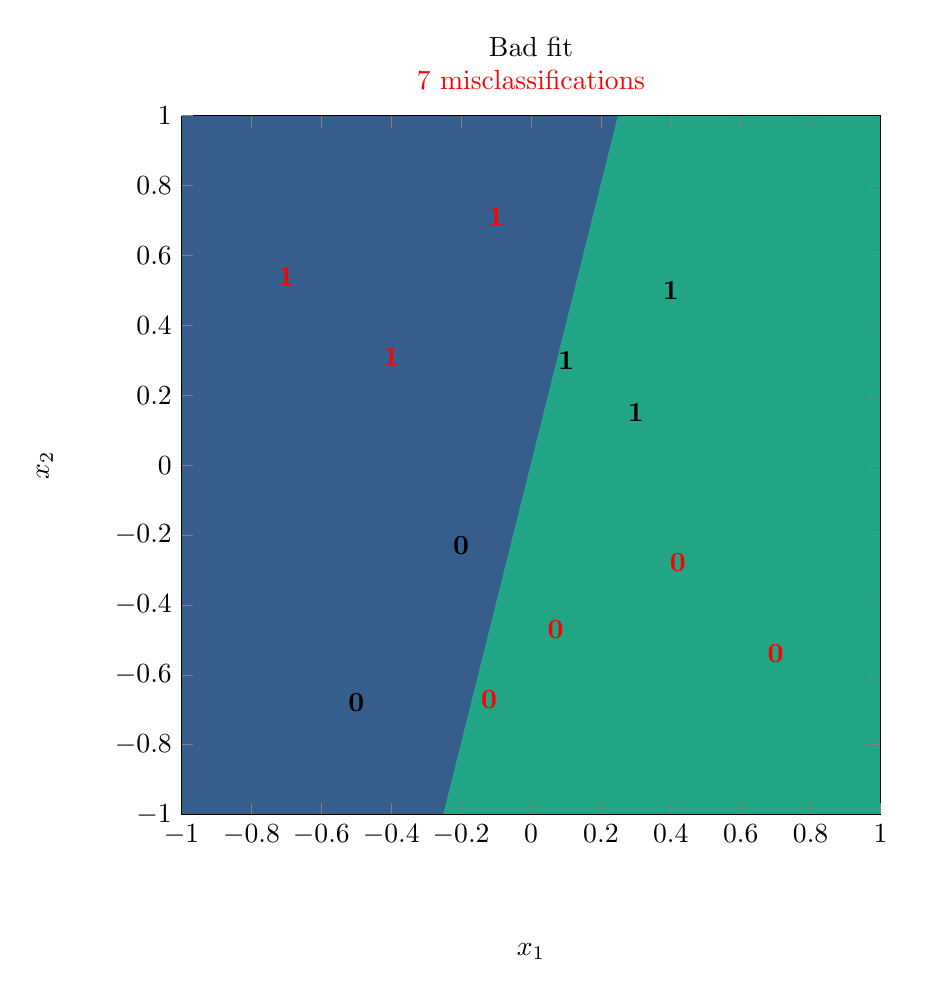
\begin{tikzpicture}
\begin{axis}[view={0}{90}, xmin=-1, xmax=1, ymin=-1, ymax=1, 
width=1.0\linewidth, xlabel=$x_1$, ylabel=$x_2$,
align=center,
title={Bad fit\\\color{red} 7 misclassifications},
axis equal image,
x label style={at={(axis description cs:0.5,-0.17)}},
y label style={at={(axis description cs:-0.17,0.5)}},
scatter/classes={%
    pos_correct={mark=text, text mark={\bf 1}},%
    pos_incorrect={mark=text, text mark={\bf \color{red} 1}},%
    neg_correct={mark=text, text mark={\bf 0}},%
    neg_incorrect={mark=text, text mark={\bf \color{red} 0}}}]
%
\addplot3[surf, shader=interp, domain=-1:1] {2*x+y};
	%\addplot[fill] {-2*x} -- cycle;
	\addplot[fill, index of colormap={5 of viridis}, color=.] coordinates 
		{(-1,-1) (-1,1) (0.25,1) (-0.25,-1)} --cycle;
	\addplot[fill, index of colormap={10 of viridis}, color=.] coordinates 
		{(0.25,1) (1,1) (1,-1) (-0.25,-1)} --cycle;

\addplot[scatter,only marks,%
    scatter src=explicit symbolic]%
table[meta=label] {
x y label
0.1 0.3 pos_correct
0.3 0.15 pos_correct
0.4 0.5 pos_correct
-0.1 0.71 pos_incorrect
-0.4 0.31 pos_incorrect
-0.7 0.54 pos_incorrect
%
-0.5 -0.68 neg_correct
-0.2 -0.23 neg_correct
-0.12 -0.67 neg_incorrect
0.07 -0.47 neg_incorrect
0.42 -0.28 neg_incorrect
0.7 -0.54 neg_incorrect
    };
\end{axis}
\end{tikzpicture}
\end{minipage}
%
%
\begin{minipage}{0.32\linewidth}
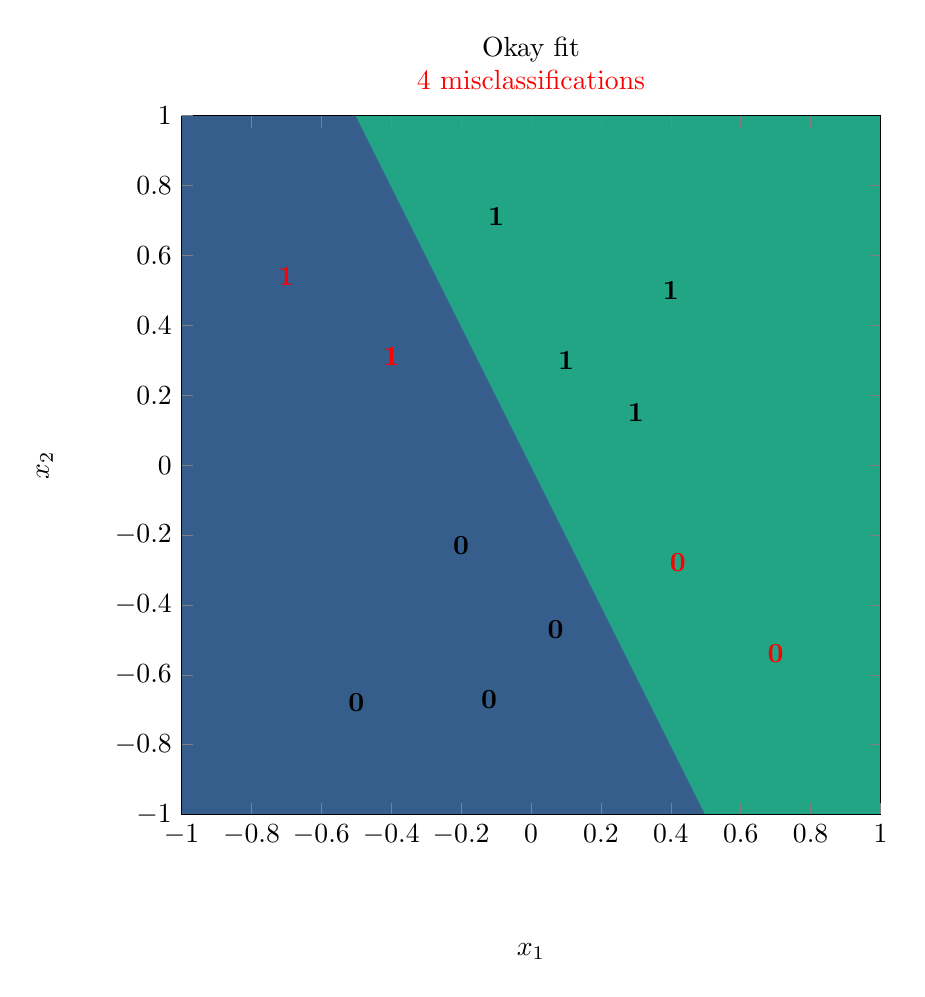
\begin{tikzpicture}
\begin{axis}[view={0}{90}, xmin=-1, xmax=1, ymin=-1, ymax=1, 
width=1.0\linewidth, xlabel=$x_1$, ylabel=$x_2$,
align=center,
title={Okay fit\\\color{red} 4 misclassifications},
axis equal image,
x label style={at={(axis description cs:0.5,-0.17)}},
y label style={at={(axis description cs:-0.17,0.5)}},
scatter/classes={%
    pos_correct={mark=text, text mark={\bf 1}},%
    pos_incorrect={mark=text, text mark={\bf \color{red} 1}},%
    neg_correct={mark=text, text mark={\bf 0}},%
    neg_incorrect={mark=text, text mark={\bf \color{red} 0}}}]
%
\addplot3[surf, shader=interp, domain=-1:1] {2*x+y};
	%\addplot[fill] {-2*x} -- cycle;
	\addplot[fill, index of colormap={5 of viridis}, color=.] coordinates 
		{(-1,-1) (0.5,-1) (-0.5,1) (-1,1)} --cycle;
	\addplot[fill, index of colormap={10 of viridis}, color=.] coordinates 
		{(0.5,-1) (1,-1) (1,1) (-0.5,1)} --cycle;
%
\addplot[scatter,only marks,%
    scatter src=explicit symbolic]%
table[meta=label] {
x y label
0.1 0.3 pos_correct
0.3 0.15 pos_correct
0.4 0.5 pos_correct
-0.1 0.71 pos_correct
-0.4 0.31 pos_incorrect
-0.7 0.54 pos_incorrect
%
-0.12 -0.67 neg_correct
-0.2 -0.23 neg_correct
-0.5 -0.68 neg_correct
0.07 -0.47 neg_correct
0.42 -0.28 neg_incorrect
0.7 -0.54 neg_incorrect
    };
\end{axis}
\end{tikzpicture}
\end{minipage}
%
%
\begin{minipage}{0.32\linewidth}
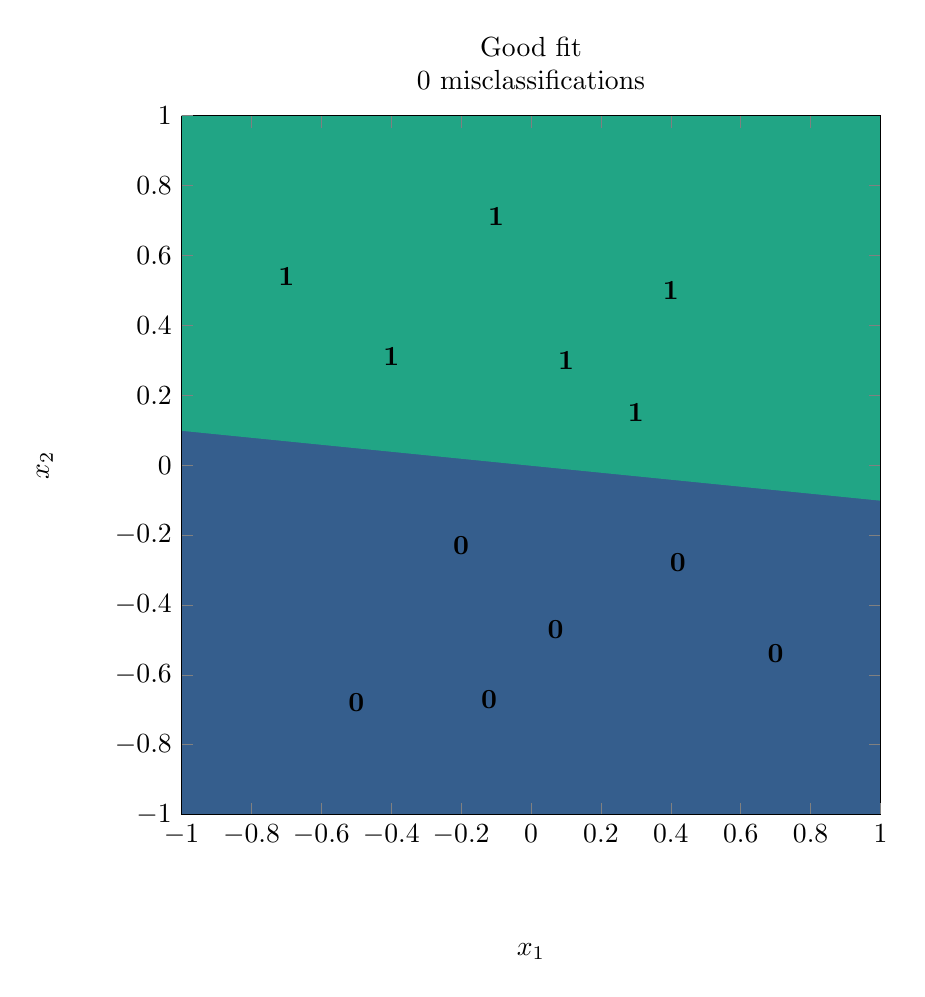
\begin{tikzpicture}
\begin{axis}[view={0}{90}, xmin=-1, xmax=1, ymin=-1, ymax=1, 
width=1.0\linewidth, xlabel=$x_1$, ylabel=$x_2$,
align=center,
title={Good fit\\0 misclassifications},
axis equal image,
x label style={at={(axis description cs:0.5,-0.17)}},
y label style={at={(axis description cs:-0.17,0.5)}},
scatter/classes={%
    pos_correct={mark=text, text mark={\bf 1}},%
    pos_incorrect={mark=text, text mark={\bf \color{red} 1}},%
    neg_correct={mark=text, text mark={\bf 0}},%
    neg_incorrect={mark=text, text mark={\bf \color{red} 0}}}]
%
\addplot3[surf, shader=interp, domain=-1:1] {2*x+y};
	%\addplot[fill] {-2*x} -- cycle;
	\addplot[fill, index of colormap={5 of viridis}, color=.] coordinates 
		{(-1,-1) (1,-1) (1,-0.1) (-1,0.1)} --cycle;
	\addplot[fill, index of colormap={10 of viridis}, color=.] coordinates 
		{(-1,0.1) (-1,1) (1,1) (1,-0.1)} --cycle;
%
\addplot[scatter,only marks,%
    scatter src=explicit symbolic]%
table[meta=label] {
x y label
0.1 0.3 pos_correct
0.3 0.15 pos_correct
0.4 0.5 pos_correct
-0.1 0.71 pos_correct
-0.4 0.31 pos_correct
-0.7 0.54 pos_correct
%
-0.12 -0.67 neg_correct
-0.2 -0.23 neg_correct
-0.5 -0.68 neg_correct
0.07 -0.47 neg_correct
0.42 -0.28 neg_correct
0.7 -0.54 neg_correct
    };
\end{axis}
\end{tikzpicture}
\end{minipage}
\caption{Different possible decision surfaces of a perceptron.}
\label{fig:neural_nets:fitting_a_perceptron}
\end{figure}

You might be wondering, what's the exact optimization algorithm that will find the best line that separates the classes? The original perceptron paper proposed one particular algorithm, the ``perceptron learning algorithm.'' This was an optimizer tailored to the specific structure of the perceptron. Older papers on neural nets are full of specific learning rules for specific architectures: the delta rule, the Rescorla-Wagner model, and so forth~\cite{rescorla1972theory}. Nowadays we rarely use these special-purpose algorithms. Instead, we use \textit{general-purpose} optimizers like gradient descent (for differentiable objectives) or zeroth-order methods (for nondifferentiable objectives). The next chapter will cover the backpropagation algorithm, which is a general-purpose gradient-based optimizer that applies to essentially all neural networks we will see in this book (but, note that for the perceptron objective, because it has a nondifferentiable threshold function, we would instead opt for a zeroth order optimizer).

\section{Multilayer Perceptrons}
Perceptrons can solve linearly separable binary classification problems, but they are otherwise rather limited. For one, they only produce a single output. What if we want multiple outputs? We can achieve this by adding edges that fan out after the perceptron (\fig{\ref{fig:neural_nets:fan_out}}).
%What if we want to output probabilities for $k$ different classes?
%What if we want to output continuous values rather than just zeros and ones? This brings us to the general purpose neuron that is the building block of almost all modern neural nets:
\begin{figure}[h]
\centerline{
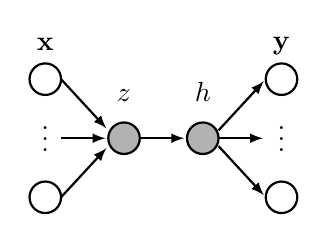
\begin{tikzpicture}[>=spaced latex]
\draw [thick] (0,-0.75) circle [radius=0.2] node[label={$\mathbf{x}$}] at (0,0.85) {};
\draw [thick] (0,0.1) node {$\vdots$};
\draw [thick] (0,0.75) circle [radius=0.2];
\draw [thick] [nn_edge] (0.2,-0.75) -- (0.8,-0.1);
\draw [thick] [nn_edge] (0.2,0.0) -- (0.8,0.0);
\draw [thick] [nn_edge] (0.2,0.75) -- (0.8,0.1);
\draw [thick, fill=gray_neuron] (1,0) circle [radius=0.2]  node[label={$z$}] at (1.0,0.2) {};
\draw [thick] [nn_edge] (1.2,0.0) -- (1.8,0.0);
\draw [thick, fill=gray_neuron] (2.0,0) circle [radius=0.2]  node[label={$h$}] at (2.0,0.2) {};
\draw [thick] [nn_edge] (2.2,-0.1) -- (2.8,-0.75);
\draw [thick] [nn_edge] (2.2,0.0) -- (2.8,0.0);
\draw [thick] [nn_edge] (2.2,0.1) -- (2.8,0.75);
\draw [thick] (3.0,-0.75) circle [radius=0.2] node[label={$\mathbf{y}$}] at (3.0,0.8) {};
\draw [thick] (3.0,0.1)  node {$\vdots$};
\draw [thick] (3.0,0.75) circle [radius=0.2];
\end{tikzpicture}
}
\caption{Multiple outputs fan out from a neuron.}
\label{fig:neural_nets:fan_out}
\end{figure}

This network maps an input {\bf layer} of data $\mathbf{x}$ to a layer of outputs {\bf y}. The neurons in between inputs and outputs are called {\bf hidden units}, shaded in gray. Here, $z$ is a \index{Preactivaton unit}{\bf preactivation} hidden unit and $h$ is a \index{Postactivation unit}{\bf postactivation} hidden unit, that is, $h = g(z)$ where $g(\cdot)$ is an activation function like in \eqn{\ref{eqn:neural_nets:perceptron_activation}}.

More commonly we might have many hidden units in stack, which we call a \index{Hidden layer}{\bf hidden layer} (\fig{\ref{fig:neural_nets:MLP1}}).
%The diagram above has one hidden layer, with a single neuron $h$, called a {\bf hidden unit}
\begin{figure}[h]
\centerline{
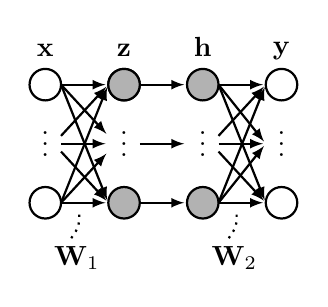
\begin{tikzpicture}[>=spaced latex]
\draw [thick] (0,-0.75) circle [radius=0.2] node[label={$\mathbf{x}$}] at (0,0.85) {};
\draw [thick] (0,0.1) node {$\vdots$};
\draw [thick] (0,0.75) circle [radius=0.2];

\draw [thick,dotted] (0.33,-1.2)  .. controls (0.43,-1.05) .. (0.43,-0.9);
\draw (0.4,-1.45) node {$\mathbf{W}_1$};

\draw [thick] [nn_edge] (0.2,-0.75) -- (0.8,-0.1);
\draw [thick] [nn_edge] (0.2,-0.75) -- (0.8,-0.75);
\draw [thick] [nn_edge] (0.2,-0.75) -- (0.8,0.75);
\draw [thick] [nn_edge] (0.2,-0.1) -- (0.8,-0.75);
\draw [thick] [nn_edge] (0.2,0.0) -- (0.8,0.0);
\draw [thick] [nn_edge] (0.2,0.1) -- (0.8,0.75);
\draw [thick] [nn_edge] (0.2,0.75) -- (0.8,0.75);
\draw [thick] [nn_edge] (0.2,0.75) -- (0.8,-0.75);
\draw [thick] [nn_edge] (0.2,0.75) -- (0.8,0.1);
\draw [thick, fill=gray_neuron] (1,0.75) circle [radius=0.2]  node[label={$\mathbf{z}$}] at (1.0,0.85) {};
\draw [thick] (1,0.1) node {$\vdots$};
\draw [thick, fill=gray_neuron] (1,-0.75) circle [radius=0.2];
\draw [thick] [nn_edge] (1.2,0.75) -- (1.8,0.75);
\draw [thick] [nn_edge] (1.2,0.0) -- (1.8,0.0);
\draw [thick] [nn_edge] (1.2,-0.75) -- (1.8,-0.75);
\draw [thick, fill=gray_neuron] (1,0.75) circle [radius=0.2]  node[label={$\mathbf{h}$}] at (2.0,0.85) {};
\draw [thick, fill=gray_neuron] (2.0,0.75) circle [radius=0.2];
\draw [thick] (2.0,0.1) node {$\vdots$};
\draw [thick, fill=gray_neuron] (2.0,-0.75) circle [radius=0.2];

\draw [thick,dotted] (2.33,-1.2)  .. controls (2.43,-1.05) .. (2.43,-0.9);
\draw (2.4,-1.45) node {$\mathbf{W}_2$};

\draw [thick] [nn_edge] (2.2,-0.75) -- (2.8,-0.75);
\draw [thick] [nn_edge] (2.2,-0.75) -- (2.8,0.75);
\draw [thick] [nn_edge] (2.2,-0.75) -- (2.8,0.0);
\draw [thick] [nn_edge] (2.2,-0.1) -- (2.8,-0.75);
\draw [thick] [nn_edge] (2.2,0.0) -- (2.8,0.0);
\draw [thick] [nn_edge] (2.2,0.1) -- (2.8,0.75);
\draw [thick] [nn_edge] (2.2,0.75) -- (2.8,0.75);
\draw [thick] [nn_edge] (2.2,0.75) -- (2.8,-0.75);
\draw [thick] [nn_edge] (2.2,0.75) -- (2.8,0.0);
\draw [thick] (3.0,-0.75) circle [radius=0.2] node[label={$\mathbf{y}$}] at (3.0,0.8) {};
\draw [thick] (3.0,0.1)  node {$\vdots$};
\draw [thick] (3.0,0.75) circle [radius=0.2];
\end{tikzpicture}
}
\caption{Mutilayer perceptron.}
\label{fig:neural_nets:MLP1}
\end{figure}
\marginnote{How many layers does this net have? Some texts will say two [$\mathbf{W}_1$, $\mathbf{W}_2$], others three [$\mathbf{x}$, $\{\mathbf{z}, \mathbf{h}\}$, $\mathbf{y}$], others four [$\mathbf{x}$, $\mathbf{z}$, $\mathbf{h}$, $\mathbf{y}$]. We must get comfortable with the ambiguity.}[2cm]
% In biology, $h_i$ and $y_i$ are two parts of a single neuron, but often in artificial neural nets we call each node in these diagrams a ``neuron".

Because this network has multiple layers of neurons, and because each neuron in this net acts as a perceptron, we call it a \index{Multilayer perceptron}\textbf{multilayer perceptron} (\textbf{MLP}). The equation for this MLP is:
\begin{align}
    \mathbf{z} &= \mathbf{W}_1\mathbf{x} + \mathbf{b}_1 &\triangleleft \quad \text{linear layer}\\
    \mathbf{h} &= g(\mathbf{z}) &\triangleleft \quad \text{activation function}\\
    \mathbf{y} &= \mathbf{W}_2\mathbf{h} + \mathbf{b}_2 &\triangleleft \quad \text{linear layer}
\end{align}
In general, MLPs can be constructed with any number of layers following this pattern: linear layer, activation function, linear layer, activation function, and so on.

The activation function $g$ could be the threshold function like in \eqn{\ref{eqn:neural_nets:perceptron_activation}}, but more generally it can be any pointwise nonlinearity, that is, $g(\mathbf{h}) = [\tilde{g}(h_1), \ldots, \tilde{g}(h_N)]$ and $\tilde{g}$ is any nonlinear function that maps $\mathbb{R} \rightarrow \mathbb{R}$.

Beyond MLPs, this kind of sequence (linear layer, pointwise nonlinearity, linear layer, pointwise nonlinearity, and so on) is the prototpyical motif in almost all neural networks, including most we will see later in this book.

\section{Activations Versus Parameters}

When working with deep nets it's useful to distinguish \emph{activations} and \emph{parameters}. The activations are the values that the neurons take on, $[\mathbf{x}, \mathbf{z}_1, \mathbf{h}_1, \ldots, \mathbf{z}_{L-1}, \mathbf{h}_{L-1}, \mathbf{y}]$; slightly abusing notation, we use this term for both preactivation function neurons and postactivation function neurons. The activations are the neural representations of the data being processed. Often, we will not worry about distinguishing between inputs, hidden units, and outputs to the net, and simply refer to all data and neural activations in a network, layer by layer, as a sequence $[\mathbf{x}_0, \ldots, \mathbf{x}_L]$, in which case $\mathbf{x}_0$ is the raw input data.

\marginnote{
A multilayer network is a sequence of transformations $f_1, \ldots, f_L$ that produce a series of activations $\mathbf{x}_1, \ldots, \mathbf{x}_L$: 
\\[6pt]
\begin{center}
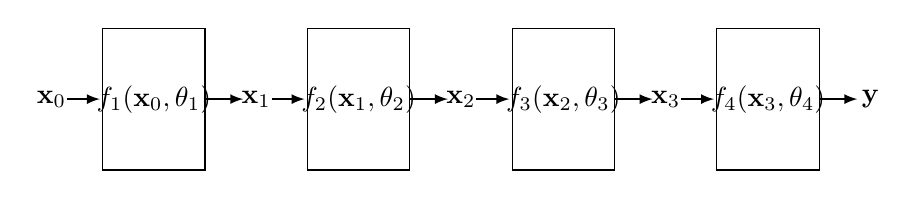
\begin{tikzpicture}
    \def\layerheight{0.8}
    \def\layerwidth{1.3}
    \def\blockheight{1.8}
    \def\blockwidth{1.3}
    % draw f's
    \foreach \x in {0,1,2,3} {
        \pgfmathsetmacro{\index}{int(\x+1)}
        \draw [fill=white] (2*\layerwidth*\x,-0.5*\blockheight) rectangle ++(\blockwidth,\blockheight) node[midway] {$f_{\index}(\mathbf{x}_{\x}, \theta_{\index})$};
    }
    % draw x's
    \foreach \x in {0,1,2,3} {
        \pgfmathsetmacro{\index}{int(\x+1)}
        \draw (2*\layerwidth*\x+0.5*\blockwidth-\layerwidth,0) node {$\mathbf{x}_\x$}; 
    }
    % draw arrows
    %\foreach \x in {0,1,2,3,4,5,6} {
    \foreach \x in {0,2,4,6} {
        %\draw [thick] [nn_edge] (0,\layerheight*\x+\blockheight) -- (0,\layerheight*\x+\layerheight);
        \draw [thick] [nn_edge] (\layerwidth*\x+\blockwidth,0) -- (\layerwidth*\x+\blockwidth+0.4*\layerwidth,0);
        \draw [thick] [nn_edge] (\layerwidth*\x+\blockwidth+0.65*\layerwidth-2*\layerwidth,0) -- (\layerwidth*\x+\blockwidth+\layerwidth-2*\layerwidth,0);
    }
    %\draw [thick] [nn_edge] (0,\layerheight*-1+\blockheight) -- (0,\layerheight*-1+\layerheight);
    \draw (7*\layerwidth+0.5*\blockwidth,0) node {$\mathbf{y}$}; 
\end{tikzpicture}
\end{center}
}[-2.2cm]

Conversely, parameters are the weights and biases of the network. These are the variables being learned. Both activations and parameters are tensors of variables.

Often we think of a layer as a function $\mathbf{x}_{l+1} = f_{l+1}(\mathbf{x}_l)$, but we can also make the parameters explicit and think of each layer as a function:
\begin{align}
    \mathbf{x}_{l+1} = f_{l+1}(\mathbf{x}_{l}, \theta_{l+1})
\end{align}
That is, each layer takes the activations from the previous layer, as well as parameters of the current layer as input, and produces activations of the next layer. Varying either the input activations or the input parameters will affect the output of the layer. From this perspective, anything we can do with parameters, we can do with activations instead, and vice versa, and that is the basis for a lot of applications and tricks. For example, while normally we learn the values of the parameters, we could instead hold the parameters fixed and learn the values of the activations that achieve some objective. In fact, this is what is done in many methods such as network prompting, adversarial attacks, and network visualization, which we will see in more detail in later chapters.
% \subsection{Data vs parameters}

% When working with deep nets it's useful to distinguish \emph{data} and \emph{parameters}. The ``data" are the values that the nodes take on, $[\mathbf{x}, \mathbf{z}_1, \mathbf{h}_1, \ldots, \mathbf{z}_{L-1}, \mathbf{h}_{L-1}, \mathbf{y}]$. It may seem strange at first to call all these variables data, but the idea is that all these values are \textit{representations} of the signal being processed. The inputs $\mathbf{x}$ are a ``raw" representation of the signal whereas later layers of neurons are transformed representations. Often, we will not worry about distinguishing between inputs, hidden units, and outputs, and simply refer to the data in a network, layer by layer, as a sequence $[\mathbf{x}_1, \ldots, \mathbf{x}_L]$.

% Parameters are the weights and biases mentioned above. These are the variables being learned. Both data and parameters are tensors of variables.

% Often we think of a layer as a function $\mathbf{x}_{l+1} = f_{l+1}(\mathbf{x}_l)$, but we can also make the parameters explicit and think of each layer as a function:
% \begin{align}
%     \mathbf{x}_{l+1} = f_{l+1}(\mathbf{x}_{l}, \theta_{l+1})
% \end{align}
% That is, each layer takes the data from the previous layer, as well as parameters of the current layer as input, and produces data of the next layer. Varying either the input data or the input parameters will affect the output of the layer. From this perspective, anything we can do with parameters, we can do with data instead, and vice versa, and that is the basis for a lot of applications and tricks. For example, while normally we learn the values of the parameters, we could instead hold the parameters fixed and learn the values of the data that achieve some objective. In fact this is what is done in applications such as style transfer, adversarial attacks, and network visualization, which we will see in more detail in later chapters.


\subsection{Fast Activations and Slow Parameters}%{\small [Advanced topic]}}
So what's different about activations versus parameters? One way to think about it is that activations are \textit{fast} functions of a data\textit{point}: they are the result of a few layers of processing this datapoint. Parameters are \textit{also} functions of the data (they are learned from data) but they are \textit{slow} functions of data\textit{sets}: the parameters are arrived at via an optimization procedure over a whole dataset. So, both activations and parameters are statistics of the data, that is, information extracted about about the data that organizes or summarizes it. The parameters are a kind of metasummary since they specify a functional transformation that produces activations from data, and activations themselves are a summary of the data. \Fig{\ref{fig:neural_nets:params_vs_activations}} shows how this looks.
\begin{figure}[h]
\centerline{
\includegraphics[width=0.7\linewidth]{figures/neural_nets/params_vs_activations.pdf}
}
\caption{Learning is a function that maps a dataset to parameters. Inference, through a neural net, is a function that maps a datapoint to activations.}
\label{fig:neural_nets:params_vs_activations}
\end{figure}

\section{Deep Nets}
Deep nets are neural nets that stack the linear-nonlinear motif many times (\fig{\ref{fig:deep_nets}}):
\begin{figure}[h]
    \centerline{
    \includegraphics[width=0.65\linewidth]{./figures/neural_nets/deep_nets.pdf}
    }
    \caption{Deep nets consist of linear layers interleaved with nonlinearities.}
    \label{fig:deep_nets}
\end{figure}

Each layer is a function. Therefore, a deep net is a composition of many functions:
\begin{align}
    f(\mathbf{x}) = f_{L}(f_{L-1}(\ldots f_2(f_1(\mathbf{x}))))
\end{align}\marginnote{The $L$ is the number of layers in the net.}[-0.5cm]
These functions are parameterized by weights $[\mathbf{W}_1, \ldots, \mathbf{W}_L]$ and biases $[\mathbf{b}_1, \ldots, \mathbf{b}_L]$. Some layers we will see later have other parameters. Collectively, we will refer to the concatenation of all the parameters in a deep net as $\theta$. %A deep net with the pattern above, that simply alternates linear layers with pointwise non-linearities is called a {\bf multi-layer perceptron}, or {\bf MLP}, as it is can be considered as a set of perceptrons stacked in sequence.

Deep nets are powerful because they can perform nonlinear mappings. In fact, a deep net with sufficiently many neurons can fit almost any desired function arbitrarily closely, a property we will investigate further in \sect{\ref{sec:neural_nets:universal_approximation}}. %The {\bf universal approximation theorem}~\cite{Cybenko1989} states that this is true even for a network with just a single hidden layer. The caveat is that the number of neurons in the hidden layers will have to be very large in order to fit complicated functions. Also, technically, this theorem only holds for continuous functions on compact subsets of $\mathbb{R}^N$ -- for example a neural net cannot fit non-computable functions.


\subsection{Deep Nets Can Perform Nonlinear Classification}

Let's return to our binary classification problem shown previously, but now let's make the two classes not linearly separable. Our new dataset is shown in \fig{\ref{fig:neural_nets:nonseparable_dataset}}.
\begin{figure}[h]
\noindent\hspace{0.3\linewidth}
\begin{minipage}{0.33\linewidth}
\begin{tikzpicture}
\begin{axis}[view={0}{90}, xmin=-1, xmax=1, ymin=-1, ymax=1, 
width=1.0\linewidth, xlabel=$x_1$, ylabel=$x_2$,
align=center,
title={},
axis equal image,
x label style={at={(axis description cs:0.5,-0.17)}},
y label style={at={(axis description cs:-0.17,0.5)}},
%x label style={at={(axis description cs:0.5,0.0)}},
%y label style={at={(axis description cs:0.2,0.5)}},
scatter/classes={%
    pos_correct={mark=text, text mark={\bf 1}},%
    pos_incorrect={mark=text, text mark={\bf \color{red} 1}},%
    neg_correct={mark=text, text mark={\bf 0}},%
    neg_incorrect={mark=text, text mark={\bf \color{red} 0}}}]
%
\addplot[scatter,only marks,%
    scatter src=explicit symbolic]%
table[meta=label] {
x y label
0.1 0.3 neg_correct
0.6 0.15 neg_correct
0.4 0.5 neg_correct
-0.1 0.71 neg_correct
-0.4 0.31 neg_correct
-0.7 0.54 neg_correct
%
0.12 -0.67 pos_correct
-0.34 -0.23 neg_correct
-0.78 -0.68 neg_correct
.84 -0.2 neg_correct
-0.18 -0.5 pos_correct
0.47 -0.64 pos_correct
0.22 -0.28 pos_correct
0.7 -0.54 pos_correct
    };
\end{axis}
\end{tikzpicture}
\end{minipage}
\caption{Dataset that is not linearly separable.}
\label{fig:neural_nets:nonseparable_dataset}
\end{figure}

Here there is no line that can separate the zeros from the ones. Nonetheless, we will demonstrate a multilayer network that can solve this problem. The trick is to just add more layers! We will use the two layer MLP shown in \fig{\ref{fig:neural_nets:simple_MLP_network}}.

\begin{figure}[h]
\centerline{

\noindent\hspace{0.05\linewidth}
\begin{minipage}{.45\linewidth}

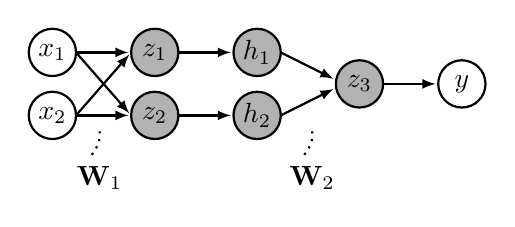
\begin{tikzpicture}[>=spaced latex]
\draw [thick] (0,-0.4) circle [radius=0.3] node {$x_2$};
\draw [thick] (0,0.4) circle [radius=0.3] node {$x_1$};
\draw [thick] [nn_edge] (0.3,-0.4) -- (1.0,-0.4);
\draw [thick] [nn_edge] (0.3,0.4) -- (1.0,0.4);
\draw [thick] [nn_edge] (0.3,-0.4) -- (1.0,0.4);
\draw [thick] [nn_edge] (0.3,0.4) -- (1.0,-0.4);
\draw [thick, fill=gray_neuron] (1.3,-0.4) circle [radius=0.3] node {$z_2$};
\draw [thick, fill=gray_neuron] (1.3,0.4) circle [radius=0.3] node {$z_1$};
\draw [thick,dotted] (0.5,-0.9)  .. controls (0.6,-0.75) .. (0.6,-0.6);
\draw (0.6,-1.2) node {$\mathbf{W}_1$};

\draw [thick] [nn_edge] (1.6,-0.4) -- (2.3,-0.4);
\draw [thick] [nn_edge] (1.6,0.4) -- (2.3,0.4);
\draw [thick, fill=gray_neuron] (2.6,-0.4) circle [radius=0.3] node {$h_2$};
\draw [thick, fill=gray_neuron] (2.6,0.4) circle [radius=0.3] node {$h_1$};
\draw [thick,dotted] (3.2,-0.9)  .. controls (3.3,-0.75) .. (3.3,-0.6);
\draw (3.3,-1.2) node {$\mathbf{W}_2$};

\draw [thick] [nn_edge] (2.9,-0.4) -- (3.6,-0.05);
\draw [thick] [nn_edge] (2.9,0.4) -- (3.6,0.05);
\draw [thick, fill=gray_neuron] (3.9,0) circle [radius=0.3] node {$z_3$};
\draw [thick] [nn_edge] (4.2,0) -- (4.9,0);
\draw [thick] (5.2,0) circle [radius=0.3] node {$y$};
\end{tikzpicture}
\caption{A simple MLP network.}
\label{fig:neural_nets:simple_MLP_network}
\end{minipage}
}
\end{figure}

Consider using the following settings for $\mathbf{W}_1$ and $\mathbf{W}_2$:
\begin{align}
    \mathbf{W}_1 = 
        \begin{bmatrix}
            -1 & 1 \\
            1 & 2
        \end{bmatrix}
    ,\quad\quad
    \mathbf{W}_2 = 
        \begin{bmatrix}
            1 & -1
        \end{bmatrix}
\end{align}
The full net then performs the following operation:
\begin{align}
    z_1 &= x_1 - x_2, \quad z_2 = 2x_1 + x_2 &\triangleleft \quad \texttt{linear}\\
    h_1 &= \max(z_1,0), \quad h_2 = \max(z_2,0) &\triangleleft \quad \texttt{relu}\\
    z_3 &= h_1-h_2 &\triangleleft \quad \texttt{linear}\\
    y &= \mathbbm{1}(z_3 > 0) &\triangleleft \quad \text{\texttt{threshold}}
\end{align}
\marginnote{The $\mathbbm{1}$ is the indicator function, which we define as: \begin{equation*}
    \mathbbm{1}(x) = \begin{cases}
                1 & \text{if $x$ is true} \\
                0 & \text{otherwise}
             \end{cases}
\end{equation*}}[-0.5cm]
Here we have introduced a new pointwise nonlinearity, the \index{Rectified linear unit}\textbf{Rectified linear unit} (\textbf{relu}), which is like a graded version of a threshold function, and has the advantage that it yields non-zero gradients over half its domain, thus being amenable to gradient-based learning.

We visualize the values that the neurons take on as a function of $x_1$ and $x_2$ in \fig{\ref{fig:neural_nets:simple_MLP_network_values}}.

\begin{figure}[h]
%\noindent\hspace{0.05\linewidth}
\begin{minipage}{1.0\linewidth}
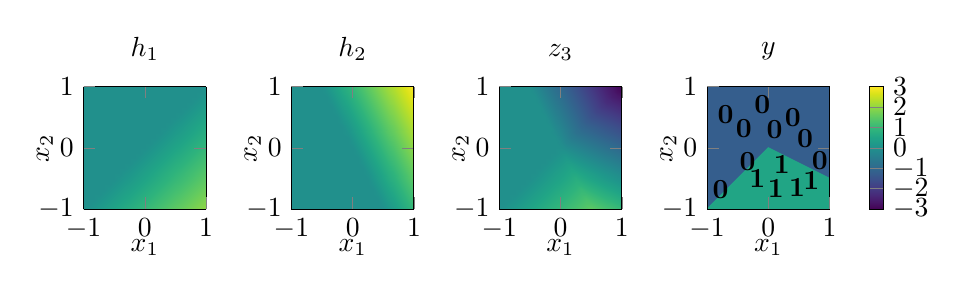
\begin{tikzpicture}
\begin{axis}[name=plot1, view={0}{90}, xmin=-1, xmax=1, ymin=-1, ymax=1, 
width=0.3\linewidth, xlabel=$x_1$, ylabel=$x_2$, 
title=$h_1$,
axis equal image,
x label style={at={(axis description cs:0.5,-0.17)}},
y label style={at={(axis description cs:-0.17,0.5)}},
point meta min=-3, point meta max=3
]
	\addplot3[surf, shader=interp, domain=-1:1] {max(-y+x,0)};
\end{axis}
\begin{axis}[name=plot2, at=(plot1.right of south east), xshift=25, view={0}{90}, xmin=-1, xmax=1, ymin=-1, ymax=1, 
width=0.3\linewidth, xlabel=$x_1$, ylabel=$x_2$, 
title=$h_2$,
axis equal image,
x label style={at={(axis description cs:0.5,-0.17)}},
y label style={at={(axis description cs:-0.17,0.5)}},
point meta min=-3, point meta max=3
]
	\addplot3[surf, shader=interp, domain=-1:1] {max(y+2*x,0)};
\end{axis}
\begin{axis}[name=plot3, at=(plot2.right of south east), xshift=25, view={0}{90}, xmin=-1, xmax=1, ymin=-1, ymax=1, 
width=0.3\linewidth, xlabel=$x_1$, ylabel=$x_2$, 
title=$z_3$,
axis equal image,
x label style={at={(axis description cs:0.5,-0.17)}},
y label style={at={(axis description cs:-0.17,0.5)}},
point meta min=-3, point meta max=3
]
	\addplot3[surf, shader=interp, domain=-1:1] {max(-y+x,0)-max(y+2*x,0)};
\end{axis}
\begin{axis}[name=plot4, at=(plot3.right of south east), xshift=25, view={0}{90}, xmin=-1, xmax=1, ymin=-1, ymax=1, 
width=0.3\linewidth, xlabel=$x_1$, ylabel=$x_2$,
title=$y$,
colorbar,
colorbar style={
        ytick={-3.0,-2.0,-1.0,0,1.0,2.0,3.0},
        yticklabel style={
            align=right
        },
        width=5.0
    },
axis equal image,
x label style={at={(axis description cs:0.5,-0.17)}},
y label style={at={(axis description cs:-0.17,0.5)}},
point meta min=-3, point meta max=3,
%ymajorticks=false
scatter/classes={%
    pos_correct={mark=text, text mark={\bf 1}},%
    pos_incorrect={mark=text, text mark={\bf \color{red} 1}},%
    neg_correct={mark=text, text mark={\bf 0}},%
    neg_incorrect={mark=text, text mark={\bf \color{red} 0}}}]
]
    \addplot3[surf, shader=interp, domain=-1:1] {max(-y+x,0)-max(y+2*x,0)};
	\addplot[fill, index of colormap={5 of viridis}, color=.] coordinates 
		{(-1,-1) (0,0) (1,-0.5) (1,1) (-1,1)} --cycle;
	\addplot[fill, index of colormap={10 of viridis}, color=.] coordinates 
		{(-1,-1) (0,0) (1,-0.5) (1,-1)} --cycle;
    \addplot[scatter,only marks,%
    scatter src=explicit symbolic]%
table[meta=label] {
x y label
0.1 0.3 neg_correct
0.6 0.15 neg_correct
0.4 0.5 neg_correct
-0.1 0.71 neg_correct
-0.4 0.31 neg_correct
-0.7 0.54 neg_correct
%
0.12 -0.67 pos_correct
-0.34 -0.23 neg_correct
-0.78 -0.68 neg_correct
.84 -0.2 neg_correct
-0.18 -0.5 pos_correct
0.47 -0.64 pos_correct
0.22 -0.28 pos_correct
0.7 -0.54 pos_correct
    };
\end{axis}
\end{tikzpicture}
\end{minipage}
\caption{Values of hidden units and output unit for the MLP shown in \fig{\ref{fig:neural_nets:simple_MLP_network}}.}
\label{fig:neural_nets:simple_MLP_network_values}
\end{figure}

As can be seen in the rightmost plot, at the output $y$, this neural net successfully assigns a value of 1 to the region of the dataspace where the datapoints labeled as 1 live. This example demonstrates that is possible to solve nonlinear classification problems with a deep net. In practice, we would want to \textit{learn} the parameter settings that achieve this classification. One way to do so would be to enumerate all possible parameter settings and pick one that successfully separates the zeros from the ones. This kind of exhaustive enumeration is a slow process, but don't worry, in \chap{\ref{chapter:backpropagation}} we will see how to speed things up using gradient descent. But it's worth remarking that enumeration is always a sufficient solution, at least when the possible parameter values form a finite set.


%\subsection{Deep nets can perform nonlinear regression}

%What about regression? It turns out deep nets are good for that too, in fact, they can be effective at implementing many kinds of functional mappings.

%Here are the functions of some random nets:

%\begin{figure}[h]
%    \centering
%    \includegraphics[width=0.19\linewidth]{figures/neural_nets/random_net1.pdf}
%    \includegraphics[width=0.19\linewidth]{figures/neural_nets/random_net2.pdf}
%    \includegraphics[width=0.19\linewidth]{figures/neural_nets/random_net3.pdf}
%    \includegraphics[width=0.19\linewidth]{figures/neural_nets/random_net4.pdf}
%    \includegraphics[width=0.19\linewidth]{figures/neural_nets/random_net5.pdf}
%    \label{fig:random_nets}
%\end{figure}

%Here's what happens as you tune one parameter. You can get it to fit all kinds of things!

\subsection{Deep Nets Are Universal Approximators}\label{sec:neural_nets:universal_approximation}
Not only can deep nets perform nonlinear classification, they can in principle perform \textit{any} continuous input-output mapping. The \index{Universal approximation theorem}{\bf universal approximation theorem}~\cite{Cybenko1989} states that this is true even for a network with just a single hidden layer. The caveat is that the number of neurons in the hidden layers will have to be very large in order to fit complicated functions.\marginnote{Technically, this theorem only holds for continuous functions on compact subsets of $\mathbb{R}^N$ -- for example a neural net cannot fit noncomputable functions. We will not be rigorous in this section. We direct the reader to \cite{TelgarskyNotes2021} for a formal treatment of universal approximation.}[-1.4cm]
%As mentioned above, this is only true if we assume the net can have an arbitrary large number of neurons. In this section we will give an intuition for why this is true.

To get an intuition for why this is true, we will consider the case of approximating an arbitrary function from $\mathbb{R} \rightarrow \mathbb{R}$ with a relu-MLP (an MLP with relu nonlinearities). First observe that any function can be approximated arbitrarily well by a sum of indicator functions, that is, bumps placed at different positions:
\begin{align}
    f(x) \approx \sum_i w_i \mathbbm{1}(\alpha_i < x < \beta_i)\label{eqn:neural_nets:sum_of_indicators}
\end{align}
As an example, in \fig{\ref{fig:neural_nets:curve_as_bump}} we show a curve (blue line) approximated in this way. As the width, $\beta-\alpha$, of the bumps (black lines) goes to zero, the error in the fit goes to zero.
\begin{figure}[h]
    \centerline{
    \includegraphics[width=0.35\linewidth]{./figures/neural_nets/curve_as_bumps.pdf}
    }
    \caption{Any function from $\mathbb{R} \rightarrow \mathbb{R}$ can be approximated arbitrarily well by a sum of elementary bumps.}
    \label{fig:neural_nets:curve_as_bump}
\end{figure}

\marginnote{While we only consider scalar functions $\mathbb{R} \rightarrow \mathbb{R}$ here, a similar construction can be used to approximate general functions of the form $\mathbb{R}^n \rightarrow \mathbb{R}^m$.}[-1.8cm]

Next we will show that a relu-MLP can represent \eqn{\ref{eqn:neural_nets:sum_of_indicators}}. The weighted sum $\sum_i w_i \ldots$ is the easy part: that's just a linear layer. So we just have to show that we can also write $\mathbbm{1}(\alpha < x < \beta)$ using linear and relu layers. It turns out the construction is rather simple:
\begin{align}
\mathbbm{1}(\alpha < x < \beta) \approx \texttt{relu}\bigg(\frac{x-(\alpha-\gamma)}{\gamma}\bigg) - \texttt{relu}\bigg(\frac{x-\alpha}{\gamma}\bigg) - \texttt{relu}\bigg(\frac{x-(\beta-\gamma)}{\gamma}\bigg) + \texttt{relu}\bigg(\frac{x-\beta)}{\gamma}\bigg) \label{eqn:neural_nets:bump_as_relu_net}
\end{align}
\marginnote{Here we show how a neural net can represent a function as a sum of basis functions. This idea is also foundational in signal processing, where signals are often represented as a sum of sine waves (\chap{\ref{chapter:fourier_analysis}}), boxes (\fig{\ref{fig:upsampling_and_downsampling:nn_interp}}), or trapezoids (\fig{\ref{fig:bilinear_interp}}).}[-2.0cm]
As $\gamma \rightarrow 0$, this approximation becomes exact. The input to each of the four relus in \eqn{\ref{eqn:neural_nets:bump_as_relu_net}} is an affine function of the input $x$, hence these four values can be represented by a linear layer with four outputs. Then we apply a relu layer to these four values, and finally we apply a linear layer to compute the sum over these relus (a weighted sum with weights [1,-1,-1,1]). Therefore \eqn{\ref{eqn:neural_nets:bump_as_relu_net}} can be implemented as a \texttt{linear}-\texttt{relu}-\texttt{linear} network. In \fig{\ref{fig:neural_nets:bump_as_relus}}, we show an example of constructing a bump in this way.
\begin{figure}[h]
    \centerline{
    \includegraphics[width=1.0\linewidth]{./figures/neural_nets/bump_as_relus.pdf}
    }
    \caption{A bump can be represented as a weighted sum of shifted and scaled relu functions.}
    \label{fig:neural_nets:bump_as_relus}
\end{figure}

Putting everything together, we have a \texttt{linear}-\texttt{relu}-\texttt{linear} for each bump, followed by a linear layer for summing up all the bumps. The two linear layers in sequence can be collapsed to a single linear layer, and hence the full function can therefore be approximated, to arbitrary precision, by a \texttt{linear}-\texttt{relu}-\texttt{linear} net.\marginnote{Most literature refers to such a net as having a single hidden layer, using the convention that we don't count pre- and postactivation neurons as separate layers.}

%The inputs to each of these $\texttt{relu}$ functions can be implemented as a linear layer (a scaling + bias), so the whole network that approximates a function as a sum of bumps is simply a linear-relu-linear net, i.e. a net with a single hidden layer. 

Notice that in this approximation, we need four relu neurons for each bump we are modeling. Therefore if we want to approximate a very bumpy function, say with $N$ bumps, we will need $4N$ relu neurons. In general, to achieve arbitrarily good approximation to a curve we may need an unbounded number of neurons in our network.

\subsection{Depth versus Width}
Above we saw that if you have a hidden layer with $N$ neurons, you can fit a scalar function with $\mathcal{O}(N)$ bumps. The number of neurons on a single hidden layer is called its \index{Network width}\textbf{width}.\marginnote{If different layers have different numbers of neurons, then we may specify the width per layer. Here we will assume all layers have the same width and simply speak of the width of the network.}[-0.4cm] So, as we increase the width of a network, we can fit ever more complicated functions. What if we instead increase the \index{Network depth}\textbf{depth} of a network, that is, its number of layers? It turns out that this can also be an effective way to increase the capacity of the net, but its effect is a bit different than increasing width.

Interestingly, it is sometimes the case that \textit{deep} nets require far fewer parameters to fit data than \textit{wide} nets. Evidence for this statement comes mostly from empiricism, where researchers have found that deeper nets just work better in practice on many popular problems. However, there is also the beginning of a mathematical theory of when and why this can happen. The basic idea of this theory is to establish that there are certain classes of function that can be represented with a polynomial number of neurons in a depth $d$ network but require an exponential number of neurons in a depth $d^\prime$ network, for certain $d^\prime < d$. Arguments along these lines are called \textbf{depth separations}, and the interested reader can refer to \cite{telgarsky2016benefits} to learn more about this ongoing line of research.

%The above argument shows that relu networks can approximate any function. There is a great deal of additional theory on exactly how many units and layers are needed to approximate exactly what kind of functions to exactly what degree of precision. One important result in this direction is Barron's theorem~\cite{barron1993universal}.

%Chapter \ref{chapter:intro_to_learning}
\section{Deep Learning: Learning with Neural Nets}
Using the formalism we defined in \chap{\ref{chapter:intro_to_learning}}, learning consists of using an \emph{optimizer} to find a function in a \emph{hypothesis space}, that maximizes an \emph{objective}. From this perspective, neural nets are simply a special kind of hypothesis space (and a particular parameterization of that hypothesis space). \index{Deep learning}\textbf{Deep learning} refers to learning algorithms that use this parameterized hypothesis space.

Deep learning also typically involves using gradient-based optimization to search the hypothesis space for the best fit to the data. We will investigate this approach in detail in \chap{\ref{chapter:backpropagation}}, where we will learn about the \textbf{backpropagation} algorithm for gradient-based learning with neural nets. However, it is certainly possible to optimize neural nets with other methods, including zeroth-order optimizers like evolution strategies (\sect{\ref{sec:gradient_descent:zeroth_order}}; \cite{salimans2017evolution}). 

One intriguing alternative to backpropagation is called \index{Hebbian learning}\textbf{Hebbian learning}~\cite{hebb2005organization}. Backpropagation is a \textit{top-down} learning algorithm, where errors incurred at the output (top) of the net are propagated backward to inform earlier layers how to update their weights and biases to minimize the loss, which is a form of learning based on \textit{feedback}. Hebbian learning, in contrast, is a \textit{bottom-up} approach, where neurons wire up just based on the \textit{feedforward} pattern of activity in the net. The canonical learning rule in Hebbian methods is \textbf{Hebb's rule}: ``fire together, wire together.'' That is, we increase the weight of the connection between two neurons whenever the two neurons are active at the same time. Although this learning rule is not explicitly minimizing a loss function, it has been shown to lead to effective neural representations. For example, Hebb-like rules can learn \textbf{infomax} representations, which capture, in the neural activations, as much information as possible about the input signal~\cite{linsker1988self}. Similar rules lead to networks that act like memory banks~\cite{hopfield1982neural}. Hebbian learning is also of interest because it is considered to be more biologically plausible than backpropagation. This is because Hebb's rule can be computed \textit{locally}—each neuron strengthens and weakens its weights based just on the activity of adjacent neurons—whereas backpropagation requires global coordination throughout the neural network. It is currently unknown how this global coordination can be achieved in biological brains.

%Indeed, it is not clear if biological neural nets actually use backpropagation. 

%Alternative optimizers include genetic algorithms~\cite{XX}, simulated annealing~\cite{XX}, and various other kinds of ``random search"~\cite{XX}.

%There is also a broad literature on ``bottom up learning rules" that do not explicitly optimize any objective (though they may implicitly). One such rule, called {\bf Hebbian learning}~\cite{hebb2005organization}, is ``fire together, wire together", that is, we increase the weight of the connection between two neurons whenever the two neurons are active at the same time.
%\marginnote{Remember, you can always just enumerate all possible parameter settings, try each, and pick the best --  smarter optimization is only about making this search faster.}

%\subsection{Classification with a deep net}
%We will now work through an example.


%\section{Regularization in neural nets}
%Weight decay, dropout


\subsection{Data Structures for Deep Learning: Tensors and Batches}

The main data structure that we will encounter in deep learning is the \index{Tensor}{\bf tensor}, which is just a multidimensional array. This may seem simple, but it's important to get comfortable with the conventions of tensor processing.

In general, everything in deep learning is represented as tensors—the input is one tensor, the activations are tensors, the weights are tensors, the outputs are tensors. If you have data that is not natively represented as a tensor, the first step, before feeding it to a deep net, is to convert it into a tensor format. Most often we use tensor of real numbers, that is, the elements of the tensor are in $\mathbb{R}$.

Suppose we have a dataset $\{\mathbf{x}^{(i)}, \mathbf{y}^{(i)}\}_{i=1}^N$ of images $\mathbf{x}$ and labels $\mathbf{y}$. The tensor way of thinking about such a dataset is as two tensors, $\mathbf{X} \in \mathbb{R}^{N \times C_0 \times H \times W }$ and $\mathbf{Y} \in \mathbb{R}^{N \times K}$. The first dimension of the tensor is the number of elements in our dataset. The remaining dimensions are the dimensionality of the images ($C_0$ color channels by height $H$ by width $W$) and labels ($K$-way classification).

The activations in the network are also tensors. For the MLP networks we have seen so far, the activation tensors have shape $N \times C_{\ell}$, where $C_{\ell}$ is the number of neurons on layer $\ell$, sometimes also called \textbf{channels} in analogy to the color channels of the input image. In later chapters we will encounter other architectures where the activation layers have additional dimensions, for example, in convolutional networks we will see activation layers that are of shape $N \times C_{\ell} \times H_{\ell} \times W_{\ell}$.

One other important concept is \index{Batch processing}{\bf batch processing}. Normally, we don't process one image at a time through a neural net. Instead we run a \textit{batch} of images all at once, and they are processed in parallel. A batch sampled from the training data can be denoted as $\{\mathbf{x}_{\texttt{batch}}^{(i)}, \mathbf{y}_{\texttt{batch}}^{(i)}\}_{i=1}^{N_{\texttt{batch}}}$, and the batch represented as a tensor has shape $\mathbf{X} \in \mathbb{R}^{N_{\texttt{batch}} \times C_0 \times H \times W}$ and $\mathbf{Y} \in \mathbb{R}^{N_{\texttt{batch}} \times K}$.

The weights and biases of the net are also usually represented as tensors. The weights and biases of a linear layer will be tensors of shape $\mathbf{W}_{\ell} \in \mathbb{R}^{C_{\ell+1} \times C_{\ell}}$ and $\mathbf{b}_{\ell} \in \mathbb{R}^{C_{\ell+1}}$.

As an example, in \fig{\ref{fig:neural_nets:simple_MLP_network_tensors_and_batches}} below, we visualize all the tensors associated with a batch of three datapoints being processed by the MLP from \fig{\ref{fig:neural_nets:simple_MLP_network}}. For this network, the input is not a set of images but instead a set of vectors $\mathbf{X} \in \mathbb{R}^{N_{\texttt{batch}} \times C_0}$. The output is one value for each input vector, so we have $\mathbf{Y} \in \mathbb{R}^{N_{\texttt{batch}} \times 1}$.

\begin{figure}[h]
\centerline{

\noindent\hspace{0.05\linewidth}
\begin{minipage}{0.65\linewidth}
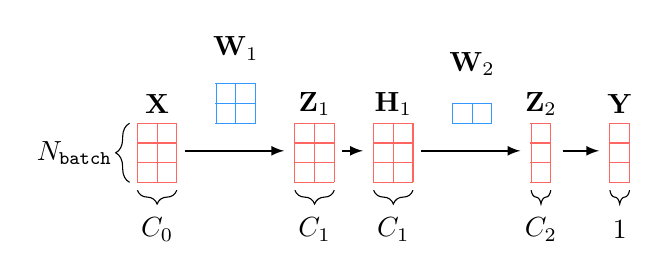
\begin{tikzpicture}
\draw[step=0.25cm,color=data_color_dark] (0,0) grid (0.5,0.75);
\draw [decorate,decoration={brace,amplitude=5pt}] (-0.1,0) -- (-0.1,0.75) node [black,midway,xshift=-0.7cm] {$N_{\texttt{batch}}$};
\draw [decorate,decoration={brace,mirror,amplitude=5pt}] (0,-0.1) -- (0.5,-0.1) node [black,midway,yshift=-0.5cm] {$C_0$};
\node at (0.25,1.0) {$\mathbf{X}$}; \draw [thick] [nn_edge] (0.6,0.4) -- (1.9,0.4);
\draw[step=0.25cm,color=param_color_dark] (0.99,0.749) grid (1.5,1.25); \node at (1.25,1.7) {$\mathbf{W}_1$};
\draw[step=0.25cm,color=data_color_dark] (1.99,0) grid (2.5,0.75); 
\draw [decorate,decoration={brace,mirror,amplitude=5pt}] (2.0,-0.1) -- (2.5,-0.1) node [black,midway,yshift=-0.5cm] {$C_1$};
\node at (2.25,1.0) {$\mathbf{Z}_1$}; \draw [thick] [nn_edge] (2.6,0.4) -- (2.9,0.4);
\draw[step=0.25cm,color=data_color_dark] (2.99,0) grid (3.5,0.75); 
\draw [decorate,decoration={brace,mirror,amplitude=5pt}] (3.0,-0.1) -- (3.5,-0.1) node [black,midway,yshift=-0.5cm] {$C_1$};
\node at (3.25,1.0) {$\mathbf{H}_1$}; \draw [thick] [nn_edge] (3.6,0.4) -- (4.9,0.4);
\draw[step=0.25cm,color=param_color_dark] (3.99,0.749) grid (4.5,1.0); \node at (4.25,1.5) {$\mathbf{W}_2$};
\draw[step=0.25cm,color=data_color_dark] (4.99,0) grid (5.25,0.75); 
\draw [decorate,decoration={brace,mirror,amplitude=5pt}] (5.0,-0.1) -- (5.25,-0.1) node [black,midway,yshift=-0.5cm] {$C_2$};
\node at (5.125,1.0) {$\mathbf{Z}_2$}; \draw [thick] [nn_edge] (5.4,0.4) -- (5.9,0.4);
\draw[step=0.25cm,color=data_color_dark] (5.99,0) grid (6.25,0.75); 
\draw [decorate,decoration={brace,mirror,amplitude=5pt}] (6.0,-0.1) -- (6.25,-0.1) node [black,midway,yshift=-0.5cm] {$1$};
\node at (6.125,1.0) {$\mathbf{Y}$};
\end{tikzpicture}
\end{minipage}
}
\caption{The tensors that represent one pass through the MLP in \fig{\ref{fig:neural_nets:simple_MLP_network}}.}
\label{fig:neural_nets:simple_MLP_network_tensors_and_batches}
\end{figure}
where the capital letters are the batches of datapoints and activations corresponding to the lowercase names of datapoints and hidden units in \fig{\ref{fig:neural_nets:simple_MLP_network}}.

This example shows the basic concept of working with tensors and batches for one-dimensional data, but, in vision, most of the time we will be working with higher-dimensional tensors. For image data we typically use four-dimensional tensors: batch $\times$ channels $\times$ height $\times$ width; for videos we may use five-dimensional tensors: batch $\times$ channels $\times$ height $\times$ width $\times$ time. Three-dimensional (3D) scans have an additional \textit{depth} spatial dimension; videos of 3D data could therefore be represented by six-dimensional tensors. As you can see, thinking in terms of two-dimensional matrices is not quite sufficient. Instead, you should be imagining data processing as operating on $N$-dimensional tensors, sliced and diced in different ways. As a step in this direction, you may find it useful to visualize tensors in 3D, as shown in \fig{\ref{fig:neural_nets:3D_tensor_example}}.
\begin{figure}[h]
\centerline{
\includegraphics[width=0.2\linewidth]{figures/neural_nets/3D_tensor_example.pdf}
}
\caption{A 3D tensor that could represent an $C \times H \times W$ color image.}
\label{fig:neural_nets:3D_tensor_example}
\end{figure}

This is closer to the actual ND tensors vision systems work with, and many concepts can be adequately captured just by thinking in 3D. We will see some examples in later chapters.

% \subsection{Batch learning}
% To train a deep net we run a batch of data through it, and then compute the loss summed (or averaged) across the batch. This scores how good the current parameter settings of the network are, as estimated on a batch of training data. We can then update the parameters (e.g., at random, or with gradient descent, which we will see in the next chapter) and try again to get a better score on the next data batch. The computational pipeline, visualized as data tensors being transformed layer by layer, looks like this:

% \noindent\hspace{0.05\linewidth}
% \begin{minipage}{0.75\linewidth}
% \begin{tikzpicture}
% \draw[step=0.25cm,color=data_color] (0,3.99) grid (0.5,4.75); \node at (0.25,5.0) {$\mathbf{X}$}; \draw [thick] [nn_edge] (0.6,4.4) -- (1.9,4.4);
% \draw[step=0.25cm,color=data_color] (1.99,3.99) grid (2.5,4.75); \node at (2.25,5.0) {$\mathbf{Z}_1$}; \draw [thick] [nn_edge] (2.6,4.4) -- (2.9,4.4);
% \draw[step=0.25cm,color=data_color] (2.99,3.99) grid (3.5,4.75); \node at (3.25,5.0) {$\mathbf{H}_1$}; \draw [thick] [nn_edge] (3.6,4.4) -- (4.9,4.4);
% \draw[step=0.25cm,color=data_color] (4.99,3.99) grid (5.25,4.75); \node at (5.125,5.0) {$\mathbf{Z}_2$}; \draw [thick] [nn_edge] (5.4,4.4) -- (5.9,4.4);
% \draw[step=0.25cm,color=data_color] (5.99,3.99) grid (6.25,4.75); \node at (6.125,5.0) {$\mathbf{Y}$};
% %
% \draw[step=0.25cm,color=data_color] (0,1.99) grid (0.5,2.75); \node at (0.25,3.0) {$\mathbf{X}$}; \draw [thick] [nn_edge] (0.6,2.4) -- (1.9,2.4);
% \draw[step=0.25cm,color=data_color] (1.99,1.99) grid (2.5,2.75); \node at (2.25,3.0) {$\mathbf{Z}_1$}; \draw [thick] [nn_edge] (2.6,2.4) -- (2.9,2.4);
% \draw[step=0.25cm,color=data_color] (2.99,1.99) grid (3.5,2.75); \node at (3.25,3.0) {$\mathbf{H}_1$}; \draw [thick] [nn_edge] (3.6,2.4) -- (4.9,2.4);
% \draw[step=0.25cm,color=data_color] (4.99,1.99) grid (5.25,2.75); \node at (5.125,3.0) {$\mathbf{Z}_2$}; \draw [thick] [nn_edge] (5.4,2.4) -- (5.9,2.4);
% \draw[step=0.25cm,color=data_color] (5.99,1.99) grid (6.25,2.75); \node at (6.125,3.0) {$\mathbf{Y}$};
% %
% \draw[step=0.25cm,color=data_color] (0,0) grid (0.5,0.75); \node at (0.25,1.0) {$\mathbf{X}$}; \draw [thick] [nn_edge] (0.6,0.4) -- (1.9,0.4);
% \draw[step=0.25cm,color=data_color] (1.99,0) grid (2.5,0.75); \node at (2.25,1.0) {$\mathbf{Z}_1$}; \draw [thick] [nn_edge] (2.6,0.4) -- (2.9,0.4);
% \draw[step=0.25cm,color=data_color] (2.99,0) grid (3.5,0.75); \node at (3.25,1.0) {$\mathbf{H}_1$}; \draw [thick] [nn_edge] (3.6,0.4) -- (4.9,0.4);
% \draw[step=0.25cm,color=data_color] (4.99,0) grid (5.25,0.75); \node at (5.125,1.0) {$\mathbf{Z}_2$}; \draw [thick] [nn_edge] (5.4,0.4) -- (5.9,0.4);
% \draw[step=0.25cm,color=data_color] (5.99,0) grid (6.25,0.75); \node at (6.125,1.0) {$\mathbf{Y}$};
% \end{tikzpicture}
% \end{minipage}


\section{Catalog of Layers}
Below, we use the color blue to denote \textcolor{param_color_dark}{\bf parameters} and the color red to denote \textcolor{data_color_dark}{\bf data/activations} (inputs and outputs to each layer).
\marginnote{We color equations in this way only in this chapter, to make clear the roles of different variables. However, be on the lookout for these colors in figures later in the book. We will often draw activations in red and parameters in blue.}[-0.4cm]

\subsection{Linear Layers}
Linear layers are the workhorses of deep nets. Almost all parameters of the network are contained in these layers; we call these parameters the weights and biases. We have already introduced linear layers previously. They look like this:
\begin{align}
    \textcolor{data_color_dark}{\xout} = \textcolor{param_color_dark}{\mathbf{W}} \textcolor{data_color_dark}{\xin} + \textcolor{param_color_dark}{\mathbf{b}} & \quad\quad \triangleleft \quad\texttt{linear}
\end{align}

\subsection{Activation Layers}

\begin{figure}[t]
    \centerline{
    \includegraphics[width=1.0\linewidth]{./figures/neural_nets/pointwise_nonlinearities.pdf}
    }
    \caption{Common pointwise nonlinearities.}
    \label{fig:neural_nets:pointwise_nonlinearities}
\end{figure}

If a net only contained linear layers then it could only compute linear functions. This is because the composition of $N$ linear functions is a linear function. \index{Activation function}\textbf{Activation layers} add nonlinearity. Activation layers are typically pointwise functions, applying a scalar to scalar mapping on each dimension of the input vector. Typically parameters of these layers, if any, are not learned (but they can be). Some common activation layers are defined below and are plotted in \fig{\ref{fig:neural_nets:pointwise_nonlinearities}}:
\begin{align}
    \textcolor{data_color_dark}{\xoutindexed}[i] &= 
        \begin{cases}
            1, &\text{if} \quad \textcolor{data_color_dark}{\xinindexed}[i] > 0\\
            0,              & \text{otherwise}
        \end{cases} & \quad\quad \triangleleft \quad \texttt{threshold}\\
    \textcolor{data_color_dark}{\xoutindexed}[i] &= \frac{1}{1 + e^{-\textcolor{data_color_dark}{\xinindexed}[i]}} & \quad\quad \triangleleft \quad \texttt{sigmoid}\\
    \textcolor{data_color_dark}{\xoutindexed}[i] &= 2*\texttt{sigmoid}(2*\textcolor{data_color_dark}{\xinindexed}[i])-1 & \quad\quad \triangleleft \quad \texttt{tanh}\\
    \textcolor{data_color_dark}{\xoutindexed}[i] &= \max(\textcolor{data_color_dark}{\xinindexed}[i],0) & \quad\quad \triangleleft \quad \texttt{relu}\\
    \textcolor{data_color_dark}{\xoutindexed}[i] &= 
        \begin{cases}
            \max(\textcolor{data_color_dark}{\xinindexed}[i],0), &\text{if} \quad \textcolor{data_color_dark}{\xinindexed}[i] \geq 0\\
            \textcolor{param_color_dark}{a}\min(\textcolor{data_color_dark}{\xinindexed}[i],0),              & \text{otherwise}
        \end{cases} & \quad\quad \triangleleft \quad \texttt{leaky-relu}
\end{align}

\subsection{Normalization Layers}\label{sec:neural_nets:normalization_layers}
\index{Normalization layers}
Normalization layers add another kind of nonlinearity. Instead of being a pointwise nonlinearity, like in activation layers, they are nonlinearities that perturb each neuron based on the collective behavior of a set of neurons. Let's start with the example of \index{Batch normalization}{\bf batch normalization} (\textbf{batchnorm})~\cite{ioffe2015batch}.

Batchnorm {\bf standardizes} each neural activation with respect to its mean and variance over a batch of datapoints. Mathematically, 
\begin{align}
    \textcolor{data_color_dark}{\xoutindexed}[i] = \textcolor{param_color_dark}{\gamma}\frac{\textcolor{data_color_dark}{\xinindexed}[i] - \mathbb{E}[\textcolor{data_color_dark}{\xinindexed}[i]]}{\sqrt{\texttt{Var}[\textcolor{data_color_dark}{\xinindexed}[i]]}} + \textcolor{param_color_dark}{\beta} & \quad\quad \triangleleft \quad \texttt{batchnorm}
\end{align}
\marginnote{Recall from statistics that the standard score of a draw of a random variable is how many standard deviations it differs from the mean: $z = \frac{x-\mu}{\sigma}$.}[-0.4cm]
where $\textcolor{param_color_dark}{\gamma}$ and $\textcolor{param_color_dark}{\beta}$ are learned parameters of this layer that maintain expressivity so that the layer can output values with non-zero mean and non-unit variance. Most commonly batchnorm is applied using training batch statistics to compute the mean and variance, which change batch to batch. At test time, aggregate statistics from the training data are used. However, using test batch statistics can be useful for achieving invariance to changes in the statistics from training data to test data~\cite{wang2020fully}.

There are numerous other normalization layers that have been defined over the years. Two more that we will highlight are \index{$L_2$ normalization}\textbf{$L_2$ normalization} and \index{Layer normalization}\textbf{layer normalization} (\textbf{layernorm})~\cite{ba2016layer}. $L_2$ normalization projects the inputs onto the unit hypersphere, which useful for bounding the activations to unit vectors:
\begin{align}
    \textcolor{data_color_dark}{\xoutindexed}[i] &= \frac{\textcolor{data_color_dark}{\xinindexed}[i]}{\norm{\textcolor{data_color_dark}{\xin}}_2} & \quad\quad \triangleleft \quad \texttt{L2-norm}
\end{align}
%This operation projects the inputs onto the unit hypersphere -- quite a nice trick.
Layernorm is similar except that it standardizes the vector of input activations:
\begin{align}
    \mu &= \frac{1}{n} \sum_{i=1}^n \textcolor{data_color_dark}{\xinindexed}[i]\\
    \sigma^2 &= \frac{1}{n} \sum_{i=1}^n (\textcolor{data_color_dark}{\xinindexed}[i] - \mu)^2\\
    \textcolor{data_color_dark}{\xoutindexed}[i] &= \textcolor{param_color_dark}{\gamma}\frac{\textcolor{data_color_dark}{\xinindexed}[i] - \mu}{\sigma} + \textcolor{param_color_dark}{\beta} & \quad\quad \triangleleft \quad \texttt{layernorm}
\end{align}
\marginnote{Notice that layernorm, like $L_2$-normalization, maps the activation vector to the surface of a hypersphere, but it also centers the activations to have zero mean, and then scales and shifts the activations via $\gamma$ and $\beta$. As an exercise, see if you can write layernorm using $L_2$-normalization as one of the steps.}[-3.2cm]
Notice that layernorm also looks quite similar to batchnorm. Both standardize activations but do so with respect to different statistics. Layernorm computes a mean and variance over elements of a datapoint $\xin$, and will do so separately for each such datapoint in a batch. Batchnorm computes the mean and variance per channel over datapoints in a batch. If we have a batch stored in the tensor $\mathbf{X} \in \mathbb{R}^{N_{\texttt{batch}} \times C}$, then what layernorm does looks just like a ``transpose'' of what batchnorm does. Batchnorm standardizes each element of the tensor by the mean and variance of its column. Layernorm standardizes each element by the mean and variance of its row:
\begin{figure}[h!]
    \centerline{
    %\noindent\hspace{0.05\linewidth}
    %\begin{minipage}{0.65\linewidth}
    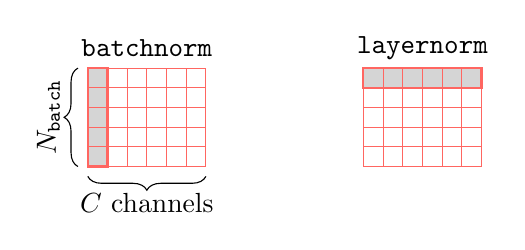
\begin{tikzpicture}
        \def\Nbatch{5}
        \def\Nchannels{6}
        \def\cellwidth{0.25}
        %
        % draw batchnorm
        \draw[step=\cellwidth,color=data_color_dark,fill=gray!33, thick] (0,0) rectangle ++(1*\cellwidth, -\Nbatch*\cellwidth);
        \draw[step=\cellwidth,color=data_color_dark] (0,0) grid (\Nchannels*\cellwidth, -\Nbatch*\cellwidth); 
        \node at (\Nchannels*0.5*\cellwidth, \cellwidth) {\texttt{batchnorm}};
        \draw [decorate,decoration={brace, amplitude=5pt, angle=0}] (\Nchannels*\cellwidth, -\Nbatch*\cellwidth-\cellwidth*0.5) -- (0, -\Nbatch*\cellwidth-\cellwidth*0.5);
        \draw (\Nchannels*0.5*\cellwidth, -\Nbatch*\cellwidth-1.85*\cellwidth) node {$C \text{ channels}$};
        \draw [decorate,decoration={brace, amplitude=5pt, angle=0}] (-\cellwidth*0.5, -\Nbatch*\cellwidth) -- (-\cellwidth*0.5, 0);
        \node [rotate=90] at (-\cellwidth*2, -\Nbatch*0.5*\cellwidth) {$N_{\texttt{batch}}$};
        %
        % draw layernorm
        \pgfmathsetmacro{\myshift}{\cellwidth*\Nchannels+2}
        \begin{scope}[xshift=\myshift cm]
            \draw[step=\cellwidth,color=data_color_dark,fill=gray!33, thick] (0,0) rectangle ++(\Nchannels*\cellwidth, -1*\cellwidth);
            \draw[step=\cellwidth,color=data_color_dark] (0,0) grid (\Nchannels*\cellwidth, -\Nbatch*\cellwidth);
            \node at (\Nchannels*0.5*\cellwidth, \cellwidth) {\texttt{layernorm}};
        \end{scope}
    \end{tikzpicture}
    %\end{minipage}
    }
    \caption{Batchnorm vs layernorm. Gray indicates the region over which mean and variance are computed. See also Figure 2 of \cite{wu2018group} for more such visualizations.}
    \label{fig:neural_nets:batchnorm_vs_layernorm_diagram}
\end{figure}

%\marginnote{See Figure 2 of \cite{wu2018group} for further normalization schemes visualized this way.}[-1cm]

One issue with batchnorm is that it requires processing a batch of datapoints all at once, and introduces a dependency between each datapoint in the batch. This violates the principle that datapoints should be processed independently and identically (iid), and this can lead to bugs if your method relies on the iid assumption. Layernorm does not have this problem and does indeed process each datapoint in an iid fashion.

\subsection{Output Layers}
The last piece we need is an \textbf{output layer} that maps a neural representation—a high-dimensional array of floating point numbers—to a desired output representation. In classification problems, the desired output is a class label, and the most common output operation is the softmax function, which we have already encountered in previous chapters. In image synthesis problems, the desired output is typically a 3D array with dimensions $N \times M \times 3$, and values in the range $[0,255]$. A sigmoid multiplied by 255 is a typical output transformation for this setting. The equations for these two layers are:
\begin{align}
    \textcolor{data_color_dark}{\xoutindexed}[i] &= \frac{e^{-\textcolor{param_color_dark}{\tau}\textcolor{data_color_dark}{\xinindexed}[i]}}{\sum_{k=1}^K e^{-\textcolor{param_color_dark}{\tau}\textcolor{data_color_dark}{\xinindexed}[k]}} & \quad\quad \triangleleft \quad \texttt{softmax}\\
    \textcolor{data_color_dark}{\xoutindexed}[i] &= 255*\texttt{sigmoid}(\textcolor{data_color_dark}{\xinindexed}[i]) & \quad\quad \triangleleft \quad \text{common layer for image output problems}
\end{align}
In the softmax definition we have added a {\bf temperature} parameter $\textcolor{param_color_dark}{\tau}$, which is used to scale how peaky, or confident, the predictions are.

The output layer is the input to the loss function, thus completing our specification of the deep learning problem. However, to use the outputs in practice requires translating them into actual pictures, or actions, or decisions. For a classification problem, this might mean taking the argmax of the softmax distribution, so that we can report a single class. For image prediction problems, it might mean rounding each output to an integral value since common image formats represent RGB values as integers.

There are of course many other output transformations you can try. Often, they will be very problem specific since they depend on the structure of the output space you are targeting.


\section{Why Are Neural Networks a Good Architecture?}
As you will soon learn, almost all modern computer vision algorithms involve deep nets in one way or another. So you may be wondering: why are deep nets such a good architecture? We will highlight here five reasons:
\begin{enumerate}
    \item They are high capacity (big enough nets are universal approximators).
    \item They are differentiable (the parameters can be optimized via gradient descent).
    \item They have good inductive biases (neural architectures reflect real structure in the world).
    \item They run efficiently on parallel hardware.
    \item They build abstractions.
\end{enumerate}
Let's look at reasons 1-3 in light of the discussion of searching for truth from \chap{\ref{chapter:problem_of_generalization}} (see \fig{\ref{fig:problem_of_generalization:search_space_tools}}). Reason 1 relates to the size of the hypothesis space. The hypothesis space can be made very big if we use a large neural network with many parameters. So we can usually be sure that our true solution (or a close approximation to it) does indeed lie in the space spanned by the neural net architecture. Reason 2 says that searching for the solution within this space is relatively easy, since we can use gradients to direct us toward ever better fits to the data. Reason 3 is one we will only come to appreciate later in the book as we investigate more advanced neural net architectures. It turns out that these architectures impose constraints and regularizers that bias our search toward solutions that capture true structure about the visual world, and this leads to learned solutions that generalize.

Reason 4 is equally important to the first three: it says we can do all of this \textit{efficiently} because most computations can be parallelized on modern hardware; in particular both matrix multiplies (linear layers) and pointwise operations (e.g., relu layers) are easy to parallelize on graphical processing units. Further, most operations are applied to image batches, where each item in the batch can be sent to a different parallel compute node.

Reason 5 is the perhaps the most subtle. It is related to the layered structure of neural nets. Layer by layer, neural nets build up increasingly abstracted representations of the input data, and these abstractions tend to be increasingly useful. This argument is not easy to appreciate at first glance, but it will be a major theme of the subsequent chapters in this book, especially those on representation learning. For now, just keep in mind that the \textit{internal representations} that are built up layer by layer in deep nets are useful and important beyond just the net's overall input-output behavior.


%and \#5 are the most subtle one, and they are the major focus of the field of neural network architecture design. In fact, the first three reasons are in a sense not so special: there are innumerable simple learning machines that all have properties 1 through 3. For example, a (distributed) lookup table has properties \#1 and \#3 and does not need property \#2 since learning is trivial (just add a row to the table for each new training point observed). What is special about neural nets is more in properties \#4 and \#5: why their architecture supports fast inference and finds solutions that generalize.


% \subsection{Depth vs width: deep nets can require fewer parameters than wide nets}
% \reviewcomment{Unfinished}

% A rule of thumb in deep learning is that bigger networks perform better. But networks can be bigger in several different ways: they can be \textit{deep} and/or they can be \textit{wide}. The \textbf{depth} of a network is its number of layers. The \textbf{width} of a network is the number of neurons on each layer (if different layers have different numbers of neurons then we may specify the width per layer). 

% Is it better to make a network deeper or wider? Universal approximation theory tells us that a sufficiently wide network can fit any function. If you are underfitting, you can add more width to increase your networks capacity and potentially fit better.

% Increasing network depth also increases its capacity, but not in quite the same way. Interestingly, it is sometimes the case that deep nets require far fewer parameters to fit data than wide nets. Evidence for this statement comes mostly from empirical practice, where researchers have found that deep nets just work better on many popular problems. 

% However, there is also the beginning of a mathematical theory of when and why this can happen. The basic idea of this theory is to establish that there are certain classes of function that can be represented with a polynomial number of neurons in a depth $d$ network but require an exponential number of neurons in a depth $d^\prime$ network, for certain $d^\prime < d$. Arguments along these lines are called \textbf{depth separations}, and the interested reader can refer to \cite{telgarsky2016benefits} to learn more about this ongoing line of research.

% %There is also the beginning of theoretical evidence for why this is the case, but this area of research is still in its infancy.

% \subsection{Deep nets are biased to find simple solutions}
% \reviewcomment{Unfinished}
% For many years, it was thought that large neural nets had far too many degrees of freedom and therefore would overfit the data they were trained one. Recall from Chapter \ref{chapter:problem_of_generalization} that the more degrees of freedom a model has (the larger its hypothesis space), the more it spurious solutions exist that fit the data but are far from the true data-generating process. However, it has by now become clear that in practice deep nets usually do \textit{not} overfit, and instead generalize remarkably well.

% Why don't deep nets overfit? An emerging explanation is that \textit{deeper nets learn simpler functions}~\cite{valle-perez, huh}. 


\section{Concluding Remarks}
Neural nets are a very simple and useful parameterized hypothesis space. They are universal approximators that can be trained via gradient descent and run on parallel hardware. \textit{Deep} nets are especially effective in computer vision; as we will soon see, deep architectures can be constructed that specifically reflect structure in the visual world, making visual processing highly efficient and performant. Artificial neural nets also have connections to the real neural nets in our brains. This connection runs deeper than merely sharing a name: the deep net architectures we will see later in this book (e.g., convolutional networks, transformers) are our best current models of computation in animal brains, in the sense that they explain brain data better than any competing models~\cite{Schrimpf2020integrative}. This is a class of models truly worth paying attention to. %Remarkably, both evolution and engineering have both arrived at a similar architecture for visual intelligence. % PHILLIP

%\setcounter{chapter}{12}
\chapter{Neural Networks as Distribution Transformers}\label{chapter:neural_nets_as_distribution_transformers}

\pgfplotsset{
    compat=1.3,
    rep2rep axis style/.style={
            width=1.0\textwidth,
            height=1.0\textwidth,
            axis lines=bottom,
            axis line style={stealth-stealth},
            y axis line style={draw=none},
            ymajorticks=false,
            xtick distance=0.5,
            tick style={draw=none},
            xmin=0,xmax=1,
            ymin=0,ymax=1,
        },
}

\section{Introduction}
So far we have seen that deep nets are stacks of simple functions, which compose to achieve interesting mappings from inputs to outputs. This section will introduce a slightly different way of thinking about deep nets. The idea is think of each layer as a \emph{geometric transformation of a data distribution}.

\section{A Different Way of Plotting Functions}
Each layer in a deep net is a mapping from one representation of the data to another: $f: \xin \rightarrow \xout$. If $\xin$ and $\xout$ are both one-dimensional (1D), then we can plot the mapping as a function with $\xin$ on the $x$-axis and $\xout$ on the $y$-axis (\fig{\ref{fig:neural_nets_as_distribution_transformers:trad_plot}}):

%\vspace{-0.5cm}
\begin{figure}[h]
\centerline{
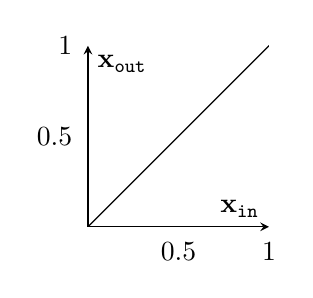
\begin{tikzpicture}
    \begin{axis}[
            width=0.32\textwidth,
            height=0.32\textwidth,
            xlabel={$\xin$},
            ylabel={$\xout$},
            axis lines=center,
            xtick distance=0.5,
            ytick distance=0.5,
            tick style={draw=none},
            xmin=0,xmax=1,
            ymin=0,ymax=1
    ]
    
    \addplot +[mark=none,smooth,black] {x};
    
    \end{axis}
\end{tikzpicture}
}
\caption{The traditional way of plotting the function $\xout = \xin$.}
\label{fig:neural_nets_as_distribution_transformers:trad_plot}
%\vspace{-0.5cm}
\end{figure}

Now, we will instead consider a different way of plotting the mapping, where we simply rotate the $y$-axis to be horizontal rather than vertical (\fig{\ref{fig:neural_nets_as_distribution_transformers:new_way_plot}}):

%\vspace{-0.5cm}
\begin{figure}[h]
\centering
\begin{minipage}[t][4.5cm][c]{0.32\textwidth}
\begin{tikzpicture}
    \begin{axis}[
            width=1.0\textwidth,
            height=1.0\textwidth,
            xlabel={$\xin$},
            ylabel={$\xout$},
            axis lines=center,
            tick style={draw=none},
            xtick distance=0.5,
            ytick distance=0.5,
            xmin=0,xmax=1,
            ymin=0,ymax=1,
    ]
    
    \addplot +[mark=none,smooth,black] {x};
    
    \addplot[scatter src=explicit symbolic, only marks, mark=triangle*, mark options={rotate=90}] coordinates {
        (0.03,0.1)
        (0.03,0.2)
        (0.03,0.3)
        (0.03,0.4)
        (0.03,0.5)
        (0.03,0.6)
        (0.03,0.7)
        (0.03,0.8)
    };
    
    \addplot[scatter src=explicit symbolic, only marks, mark=*] coordinates {
        (0.1,0)
        (0.2,0)
        (0.3,0)
        (0.4,0)
        (0.5,0)
        (0.6,0)
        (0.7,0)
        (0.8,0)
    };
    
    \addplot[mark=none,dashed] coordinates {
    	(0.1,0)
    	(0.1,0.1)
    };
    \addplot[mark=none,dashed] coordinates {
    	(0.2,0)
    	(0.2,0.2)
    };
    \addplot[mark=none,dashed] coordinates {
    	(0.3,0)
    	(0.3,0.3)
    };
    \addplot[mark=none,dashed] coordinates {
    	(0.4,0)
    	(0.4,0.4)
    };
    \addplot[mark=none,dashed] coordinates {
    	(0.5,0)
    	(0.5,0.5)
    };
    \addplot[mark=none,dashed] coordinates {
    	(0.6,0)
    	(0.6,0.6)
    };
    \addplot[mark=none,dashed] coordinates {
    	(0.7,0)
    	(0.7,0.7)
    };
    \addplot[mark=none,dashed] coordinates {
    	(0.8,0)
    	(0.8,0.8)
    };
    
    \addplot[mark=none,dashed] coordinates {
    	(0,0.1)
    	(0.1,0.1)
    };
    \addplot[mark=none,dashed] coordinates {
    	(0,0.2)
    	(0.2,0.2)
    };
    \addplot[mark=none,dashed] coordinates {
    	(0,0.3)
    	(0.3,0.3)
    };
    \addplot[mark=none,dashed] coordinates {
    	(0,0.4)
    	(0.4,0.4)
    };
    \addplot[mark=none,dashed] coordinates {
    	(0,0.5)
    	(0.5,0.5)
    };
    \addplot[mark=none,dashed] coordinates {
    	(0,0.6)
    	(0.6,0.6)
    };
    \addplot[mark=none,dashed] coordinates {
    	(0,0.7)
    	(0.7,0.7)
    };
    \addplot[mark=none,dashed] coordinates {
    	(0,0.8)
    	(0.8,0.8)
    };
    
\end{axis}
\end{tikzpicture}
\end{minipage}
\begin{minipage}[t][4.5cm][c]{0.1\textwidth}
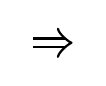
\begin{tikzpicture}
    \draw [line width=1pt, double distance=2pt, -{Classical TikZ Rightarrow[length=2mm]}] (0,0) -- (0.5,0);
\end{tikzpicture}
\end{minipage}
\begin{minipage}[t][4.5cm][c]{0.32\textwidth}
\begin{tikzpicture}
    
    % \begin{axis}[
    %         rep2rep axis style,
    %         xlabel={$\xin$},
    %         ylabel={$\xout$},
    %         axis x line=bottom, % Place the x-axis on the bottom
    %         axis y line=top,    % Place the y-axis on the top
    % ]

    \begin{axis}[
            rep2rep axis style,
            xlabel={$\xin$},
    ]
    \end{axis}
    
    \begin{axis}[
            rep2rep axis style,
            xlabel={$\xout$},
            axis lines=top,
    ]
    
    \addplot[mark=none,dashed] coordinates {
    	(0.1,0)
    	(0.1,1)
    };
    \addplot[mark=none,dashed] coordinates {
    	(0.2,0)
    	(0.2,1)
    };
    \addplot[mark=none,dashed] coordinates {
    	(0.3,0)
    	(0.3,1)
    };
    \addplot[mark=none,dashed] coordinates {
    	(0.4,0)
    	(0.4,1)
    };
    \addplot[mark=none,dashed] coordinates {
    	(0.5,0)
    	(0.5,1)
    };
    \addplot[mark=none,dashed] coordinates {
    	(0.6,0)
    	(0.6,1)
    };
    \addplot[mark=none,dashed] coordinates {
    	(0.7,0)
    	(0.7,1)
    };
    \addplot[mark=none,dashed] coordinates {
    	(0.8,0)
    	(0.8,1)
    };
    \addplot[mark=none,dashed] coordinates {
    	(0.9,0)
    	(0.9,1)
    };
    
    \addplot[scatter src=explicit symbolic, only marks, mark=*] coordinates {
        (0.1,0)
        (0.2,0)
        (0.3,0)
        (0.4,0)
        (0.5,0)
        (0.6,0)
        (0.7,0)
        (0.8,0)
        (0.9,0)
    };
    
    \addplot[scatter src=explicit symbolic, only marks, mark=triangle*] coordinates {
        (0.1,0.97)
        (0.2,0.97)
        (0.3,0.97)
        (0.4,0.97)
        (0.5,0.97)
        (0.6,0.97)
        (0.7,0.97)
        (0.8,0.97)
        (0.9,0.97)
    };
    
\end{axis}
\end{tikzpicture}
\end{minipage}
\caption{An alternative way of plotting a function (right). Functions are mappings that rearrange the input space. The identity function $\xout=\xin$, shown here, means ``no rearrangement,'' so the mapping is straight lines.}
\label{fig:neural_nets_as_distribution_transformers:new_way_plot}
%\vspace{-0.5cm}
\end{figure}

The depiction to the right makes it obvious that the plot $\xout = \xin$ is the identity mapping: datapoints get mapped to unchanged positions. \Fig{\ref{fig:neural_nets_as_distribution_transformers:new_way_plot_examples}} shows a few more mappings plotted in this way:
\begin{figure}[h]
\begin{minipage}[t][5.0cm][c]{0.45\textwidth}
%\begin{minipage}[t][5.5cm][c]{0.45\textwidth}
%\begin{flushleft}
\begin{tikzpicture}
    \begin{axis}[
            rep2rep axis style,
            width=0.78\textwidth,
            height=0.6\textwidth,
            title={$\xout = 2\xin$},
            title style={at={(0.1,0.5)},anchor=north east,draw=black,fill=white},
            xlabel={$\xin$},
            xmin=-1.2,xmax=1.2,
    ]
    \end{axis}
    
    \begin{axis}[
            rep2rep axis style,
            width=0.78\textwidth,
            height=0.6\textwidth,
            xlabel={$\xout$},
            axis lines=top,
            xmin=-1.2,xmax=1.2,
    ]
    
    \addplot[mark=none,dashed] coordinates {
    	(-0.5,0)
    	(-1.0,1)
    };
    \addplot[mark=none,dashed] coordinates {
    	(-0.25,0)
    	(-0.5,1)
    };
    \addplot[mark=none,dashed] coordinates {
    	(0,0)
    	(0,1)
    };
    \addplot[mark=none,dashed] coordinates {
    	(0.25,0)
    	(0.5,1)
    };
    \addplot[mark=none,dashed] coordinates {
    	(0.5,0)
    	(1,1)
    };
    
    \addplot[scatter src=explicit symbolic, only marks, mark=*] coordinates {
        (-0.5,0)
        (-0.25,0)
        (0,0)
        (0.25,0)
        (0.5,0)
    };
    
    \addplot[scatter src=explicit symbolic, only marks, mark=triangle*] coordinates {
        (-1,0.97)
        (-0.5,0.97)
        (0,0.97)
        (0.5,0.97)
        (1,0.97)
    };
\end{axis}
\end{tikzpicture}
%\end{flushleft}
\end{minipage}
\begin{minipage}[t][5.0cm][c]{0.45\textwidth}
%\begin{minipage}[t][5.5cm][c]{0.45\textwidth}
%\begin{flushright}
\begin{tikzpicture}
    \begin{axis}[
            rep2rep axis style,
            width=0.78\textwidth,
            height=0.6\textwidth,
            title={$\xout = \frac{\xin + 1}{2}$},
            title style={at={(0.1,0.5)},anchor=north east,draw=black,fill=white},
            xlabel={$\xin$},
            xmin=-1.2,xmax=1.2,
    ]
    \end{axis}
    
    \begin{axis}[
            rep2rep axis style,
            width=0.78\textwidth,
            height=0.6\textwidth,
            xlabel={$\xout$},
            axis lines=top,
            xmin=-1.2,xmax=1.2,
    ]
    
    \addplot[mark=none,dashed] coordinates {
    	(-1.0,0)
    	(0,1)
    };
    \addplot[mark=none,dashed] coordinates {
    	(-0.5,0)
    	(0.25,1)
    };
    \addplot[mark=none,dashed] coordinates {
    	(0,0)
    	(0.5,1)
    };
    \addplot[mark=none,dashed] coordinates {
    	(0.5,0)
    	(0.75,1)
    };
    \addplot[mark=none,dashed] coordinates {
    	(1,0)
    	(1,1)
    };
    
    \addplot[scatter src=explicit symbolic, only marks, mark=*] coordinates {
        (-1,0)
        (-0.5,0)
        (0,0)
        (0.5,0)
        (1,0)
    };
    
    \addplot[scatter src=explicit symbolic, only marks, mark=triangle*] coordinates {
        (0,0.97)
        (0.25,0.97)
        (0.5,0.97)
        (0.75,0.97)
        (1,0.97)
    };
\end{axis}
\end{tikzpicture}
%\end{flushright}
\end{minipage}
\begin{minipage}[t][5.0cm][c]{0.45\textwidth}
%\begin{flushleft}
\begin{tikzpicture}
    \begin{axis}[
            rep2rep axis style,
            width=0.78\textwidth,
            height=0.6\textwidth,
            title={$\xout = \texttt{relu}(\xin)$},
            title style={at={(0.1,0.5)},anchor=north east,draw=black,fill=white},
            xlabel={$\xin$},
            xmin=-1.2,xmax=1.2,
    ]
    \end{axis}
    
    \begin{axis}[
            rep2rep axis style,
            width=0.78\textwidth,
            height=0.6\textwidth,
            xlabel={$\xout$},
            axis lines=top,
            xmin=-1.2,xmax=1.2,
    ]
    
    \addplot[mark=none,dashed] coordinates {
    	(-1,0)
    	(0,1)
    };
    \addplot[mark=none,dashed] coordinates {
    	(-0.5,0)
    	(0,1)
    };
    \addplot[mark=none,dashed] coordinates {
    	(0,0)
    	(0,1)
    };
    \addplot[mark=none,dashed] coordinates {
    	(0.5,0)
    	(0.5,1)
    };
    \addplot[mark=none,dashed] coordinates {
    	(1,0)
    	(1,1)
    };
    
    \addplot[scatter src=explicit symbolic, only marks, mark=*] coordinates {
        (-1,0)
        (-0.5,0)
        (0,0)
        (0.5,0)
        (1,0)
    };
    
    \addplot[scatter src=explicit symbolic, only marks, mark=triangle*] coordinates {
        (0,0.97)
        (0.5,0.97)
        (0,0.97)
        (0.5,0.97)
        (1, 0.97)
    };
\end{axis}
\end{tikzpicture}
%\end{flushleft}
\end{minipage}
\begin{minipage}[t][5.0cm][c]{0.45\textwidth}
%\begin{flushright}
\begin{tikzpicture}
    \begin{axis}[
            rep2rep axis style,
            width=0.78\textwidth,
            height=0.6\textwidth,
            title={$\xout = \texttt{sigmoid}(\xin)$},
            title style={at={(0.1,0.5)},anchor=north east,draw=black,fill=white},
            xlabel={$\xin$},
            xmin=-5.2,xmax=5.2,
            xtick distance=2.5,
    ]
    \end{axis}
    
    \begin{axis}[
            rep2rep axis style,
            width=0.78\textwidth,
            height=0.6\textwidth,
            xlabel={$\xout$},
            axis lines=top,
            xmin=-1.2,xmax=1.2,
    ]
    
    \addplot[mark=none,dashed] coordinates {
    	(-1.0,0)
    	(0.007,1)
    };
    \addplot[mark=none,dashed] coordinates {
    	(-0.5,0)
    	(0.076,1)
    };
    \addplot[mark=none,dashed] coordinates {
    	(0,0)
    	(0.5,1)
    };
    \addplot[mark=none,dashed] coordinates {
    	(0.5,0)
    	(0.924,1)
    };
    \addplot[mark=none,dashed] coordinates {
    	(1,0)
    	(0.993,1)
    };
    
    \addplot[scatter src=explicit symbolic, only marks, mark=*] coordinates {
        (-1,0)
        (-0.5,0)
        (0,0)
        (0.5,0)
        (1,0)
    };
    
    \addplot[scatter src=explicit symbolic, only marks, mark=triangle*] coordinates {
        (0.007,0.97)
        (0.076,0.97)
        (0.5,0.97)
        (0.924,0.97)
        (0.993,0.97)
    };
    
\end{axis}
\end{tikzpicture}
%\end{flushright}
\end{minipage}
\caption{Mapping plots for several simple functions that could be neural layers.}
\label{fig:neural_nets_as_distribution_transformers:new_way_plot_examples}
\end{figure}

Each of the above are layers that could be found in a deep net. Linear layers, like those in the top row above, stretch and squash the data distribution. The relu nonlinearity maps all negative data to 0, and applies an identity map to all nonnegative data. The sigmoid function pulls negative data to 0 and positive data to 1.

\section{How Deep Nets Remap a Data Distribution}
In this way, an incoming data distribution can be reshaped layer by layer into a desired configuration. The goal of a binary softmax classifier, for example, is to move the datapoints around until all the class 0 points end up moved to $[1,0]$ on the output layer and all the class 1 points end up moved to $[0,1]$.
\marginnote{This is because the one-hot code for the integer 0 is $[1,0]$ and the one-hot code for the integer 1 is $[0,1]$.}[-1cm]

A deep net stacks these operations; an example is given in \fig{\ref{fig:neural_nets_as_distribution_transformers:new_way_plot_two_layer}}.
\begin{figure}[h]
%\noindent\hspace{0.25\linewidth}
\centerline{
\begin{tikzpicture}
    \begin{axis}[
            rep2rep axis style,
            width=0.35\textwidth,
            height=0.4\textwidth,
            title={$\mathbf{x}_1 = 2*\mathbf{x}_0$},
            title style={at={(0.1,0.25)},anchor=north east,draw=black,fill=white},
            xlabel={$\mathbf{x}_0$},
            xmin=-1.2,xmax=1.2,
    ]
    \end{axis}
    
    % \begin{axis}[
    %         rep2rep axis style,
    %         width=0.35\textwidth,
    %         height=0.25\textwidth,
    %         title={$\mathbf{x}^{(2)} = \texttt{relu}(\mathbf{x}^{(1)})$},
    %         title style={at={(0.1,1.5)},anchor=north east,draw=black,fill=white},
    %         xlabel={$\mathbf{x}^{(1)}$},
    %         axis lines=top,
    %         xmin=-1.2,xmax=1.2,
    % ]
    % \end{axis}
    
    \begin{axis}[
            rep2rep axis style,
            width=0.35\textwidth,
            height=0.4\textwidth,
            title={$\mathbf{x}_2 = \texttt{relu}(\mathbf{x}_1$},
             title style={at={(0.1,0.75)},anchor=north east,draw=black,fill=white},
            xlabel={$\mathbf{x}_2$},
            axis lines=top,
            xmin=-1.2,xmax=1.2,
            ymin=0,ymax=2
    ]
    
    \addplot[mark=none] coordinates {
    	(-1.2,1)
    	(1.2,1)
    };
    
    \addplot[mark=none,dashed] coordinates {
    	(-0.5,0)
    	(-1.0,1)
    };
    \addplot[mark=none,dashed] coordinates {
    	(-0.25,0)
    	(-0.5,1)
    };
    \addplot[mark=none,dashed] coordinates {
    	(0,0)
    	(0,1)
    };
    \addplot[mark=none,dashed] coordinates {
    	(0.25,0)
    	(0.5,1)
    };
    \addplot[mark=none,dashed] coordinates {
    	(0.5,0)
    	(1,1)
    };
    
    \addplot[scatter src=explicit symbolic, only marks, mark=*] coordinates {
        (-0.5,0)
        (-0.25,0)
        (0,0)
        (0.25,0)
        (0.5,0)
    };
    
    \addplot[scatter src=explicit symbolic, only marks, mark=triangle*] coordinates {
        (-1,0.97)
        (-0.5,0.97)
        (0,0.97)
        (0.5,0.97)
        (1,0.97)
    };
    
    \addplot[mark=none,dashed] coordinates {
    	(-1,1)
    	(0,2)
    };
    \addplot[mark=none,dashed] coordinates {
    	(-0.5,1)
    	(0,2)
    };
    \addplot[mark=none,dashed] coordinates {
    	(0,1)
    	(0,2)
    };
    \addplot[mark=none,dashed] coordinates {
    	(0.5,1)
    	(0.5,2)
    };
    \addplot[mark=none,dashed] coordinates {
    	(1,1)
    	(1,2)
    };
    
    \addplot[scatter src=explicit symbolic, only marks, mark=triangle*] coordinates {
        (0,1.97)
        (0,1.97)
        (0,1.97)
        (0.5,1.97)
        (1,1.97)
    };
    
\end{axis}

\end{tikzpicture}
}
\caption{Mapping plot for a \texttt{linear}-\texttt{relu} stack.}
\label{fig:neural_nets_as_distribution_transformers:new_way_plot_two_layer}
\end{figure}

The plots above show how a uniform grid of datapoints get mapped from layer to layer in a deep net. We can also use this plotting style to show how a nonuniform distribution of incoming datapoints gets transformed. This is the setting in which deep nets actually operate, and sometimes the real action of the network looks very different when viewed this way. We can think of a deep net as transforming an input data distribution, $\pdata$, into an output data distribution, $\pout$. Each layer of activations in a network is a different representation or \index{Embedding}{\bf embedding} of the data, and we can consider the distribution of activations on some layer $\ell$ to be $p_{\ell}$. Then, layer by layer, a deep net transforms $\pdata$ into $p_{\texttt{1}}$ into $p_{\texttt{2}}$, and so on until finally transforming the data to the distribution $\pout$. Most loss functions can also be interpreted from this angle: they penalize the divergence, in one form or another, between the output distribution $\pout$ and a target distribution $p_{\texttt{target}}$.

A nice property of this way of plotting is that it also extends to visualizing two-dimensional (2D)-to-2D mappings (something that conventional $x$-axis/$y$-axis plotting is not well equipped to do). Real deep nets perform $N$-dimensional (ND)-to-ND mappings, but already 2D-to-2D visualizations can give a lot of insight into the general case. In \fig{\ref{fig:neural_nets_as_data_transformations:2D_mapping_diagrams}}, we show how three common neural net layers may act to transform a Gaussian blob of data centered at the origin.
\begin{figure}[h]
\centerline{
\begin{minipage}{0.36\textwidth}
\begin{tikzpicture}
    \draw (0, 0) node[inner sep=0] {\includegraphics[width=0.8\linewidth]{figures/neural_nets/linear_layer_mapviz.pdf}};
    \draw (-1, -1.4) node {$\xin$};
    \draw (-1, 1.45) node {$\xout$};
    \draw (0, 2.3) node {\texttt{linear}};
\end{tikzpicture}
\end{minipage}
\begin{minipage}{0.28\textwidth}
\begin{tikzpicture}
    \draw (0, 0) node[inner sep=0] {\includegraphics[width=0.8\linewidth]{figures/neural_nets/relu_layer_mapviz.pdf}};
    \draw (-1.6, -1.4) node {$\xin$};
    \draw (-1.6, 1.45) node {$\xout$};
    \draw (0, 2.3) node {\texttt{relu}};
\end{tikzpicture}
\end{minipage}
\begin{minipage}{0.28\textwidth}
\begin{tikzpicture}
    \draw (0, 0) node[inner sep=0] {\includegraphics[width=0.8\linewidth]{figures/neural_nets/L2norm_layer_mapviz.pdf}};
    \draw (-1.6, -1.4) node {$\xin$};
    \draw (-1.6, 1.45) node {$\xout$};
    \draw (0, 2.3) node {\texttt{L2-norm}};
\end{tikzpicture}
\end{minipage}
% \begin{minipage}{0.33\textwidth}
% \begin{flushright}
% \begin{tikzpicture}
%     \draw (0, 0) node[inner sep=0] {\includegraphics[width=1.0\linewidth]{figures/neural_nets/softmax_layer_mapviz.pdf}};
% \end{tikzpicture}
% \end{flushright}
% \end{minipage}
}
\caption{2D mapping diagrams for several neural layers. The \texttt{linear} layer mapping will shift, stretch, and rotate depending on its weights and biases.}
\label{fig:neural_nets_as_data_transformations:2D_mapping_diagrams}
\end{figure}


%Here is a linear layer $f: \mathbb{R}^2 \rightarrow \mathbb{R}^2$:
% Here are the linear and relu layers plotted this way, alongside other ways of representing these mappings:
% \begin{figure}[h]
%     \centerline{
%     \includegraphics[width=1.0\linewidth]{./figures/neural_nets/layer_cards_linear_relu.pdf}}
%     \caption{A summary of the main two layers we have learned about so far.}
%     \label{fig:neural_nets:layer_cards_linear_relu}
% \end{figure}

One interesting thing to notice here is that the relu layer maps many points to the axes of the positive quadrant. In general, with relu-nets, a lot of data density will build up along these axes, because any point \textit{not} in the positive quadrant snaps to an axis. This effect becomes exaggerated in real networks with high-dimensional embeddings. In particular, for a width-$N$ layer, the region that is strictly positive occupies only $\frac{1}{2^N}$ proportion of the embedding space, so almost the entire space gets mapped to the axes after a relu layer. The geometry of high-dimensional neural representations may become very sparse because of this, where most of the volume of representational space is not occupied by any datapoints.
%This is because relu snaps all negative coordinates to zero, so any point in the negative subspace will end up mapping to an ``edge" of the positive quadrant.

% \begin{figure}[h]
%     \centering
%     \includegraphics[width=0.36\linewidth]{./figures/neural_nets_as_data_transformations/2D_linear_layer.png}
%     \label{fig:neural_nets_as_data_transformations:2D_linear_layer}
% \end{figure}

%The data can be thought of as itself a representation. The target output, e.g., class labels, is another representation. Then a classifier network, layer by layer, maps a representations that matches the raw data to a representation that matches the labels. The sequence of representations for an input datapoint $\xin^i$ is $\xin^i \rightarrow \mathbf{h}^{(1)i} \rightarrow \mathbf{h}^{(2)i} \rightarrow \cdots \rightarrow \xout^i$.

%One way to characterize this sequence of representations is by looking at how each subsequent layer represents an entire \emph{dataset}. 


\section{Binary Classifier Example}
Consider a multilayer perceptron (MLP) that performs binary classification formulated as two-way softmax regression. The input datapoints are each in $\mathbb{R}^2$ and the target outputs are in $\vartriangle^1$ (the one-simplex), %\marginnote{The {\bf N-simplex}, $\vartriangle^N$, is the set of all $N+1$ dimensional vectors whose elements sum to 1. $N+1$ dim one-hot codes live on the vertices of $\vartriangle^{N}$.}[-1.0cm] 
with layer structure $\texttt{linear}-\texttt{relu}-\texttt{linear}-\texttt{relu}-\texttt{linear}$. This network is drawn below in \fig{\ref{fig:neural_nets:simple_MLP_network2}}:

\begin{figure}[h]
\centerline{

%\noindent\hspace{0.05\linewidth}
%\begin{minipage}{.45\linewidth}

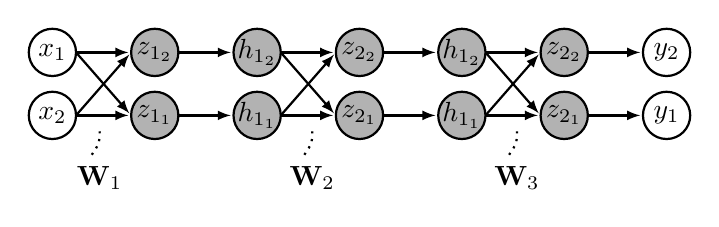
\begin{tikzpicture}[>=spaced latex]
% linear1
\draw [thick] (0,-0.4) circle [radius=0.3] node {$x_2$};
\draw [thick] (0,0.4) circle [radius=0.3] node {$x_1$};
\draw [thick] [nn_edge] (0.3,-0.4) -- (1.0,-0.4);
\draw [thick] [nn_edge] (0.3,0.4) -- (1.0,0.4);
\draw [thick] [nn_edge] (0.3,-0.4) -- (1.0,0.4);
\draw [thick] [nn_edge] (0.3,0.4) -- (1.0,-0.4);
\draw [thick, fill=gray_neuron] (1.3,-0.4) circle [radius=0.3] node {$z_{1_1}$};
\draw [thick, fill=gray_neuron] (1.3,0.4) circle [radius=0.3] node {$z_{1_2}$};
\draw [thick,dotted] (0.5,-0.9)  .. controls (0.6,-0.75) .. (0.6,-0.6);
\draw (0.6,-1.2) node {$\mathbf{W}_1$};

% relu1
\draw [thick] [nn_edge] (1.6,-0.4) -- (2.3,-0.4);
\draw [thick] [nn_edge] (1.6,0.4) -- (2.3,0.4);
\draw [thick, fill=gray_neuron] (2.6,-0.4) circle [radius=0.3] node {$h_{1_1}$};
\draw [thick, fill=gray_neuron] (2.6,0.4) circle [radius=0.3] node {$h_{1_2}$};

% linear2
\draw [thick] [nn_edge] (2.9,-0.4) -- (3.6,0.4);
\draw [thick] [nn_edge] (2.9,0.4) -- (3.6,-0.4);
\draw [thick] [nn_edge] (2.9,-0.4) -- (3.6,-0.4);
\draw [thick] [nn_edge] (2.9,0.4) -- (3.6,0.4);
\draw [thick, fill=gray_neuron] (3.9,-0.4) circle [radius=0.3] node {$z_{2_1}$};
\draw [thick, fill=gray_neuron] (3.9,0.4) circle [radius=0.3] node {$z_{2_2}$};
\draw [thick,dotted] (3.2,-0.9)  .. controls (3.3,-0.75) .. (3.3,-0.6);
\draw (3.3,-1.2) node {$\mathbf{W}_2$};

% relu2
\draw [thick] [nn_edge] (4.2,-0.4) -- (4.9,-0.4);
\draw [thick] [nn_edge] (4.2,0.4) -- (4.9,0.4);
\draw [thick, fill=gray_neuron] (5.2,-0.4) circle [radius=0.3] node {$h_{1_1}$};
\draw [thick, fill=gray_neuron] (5.2,0.4) circle [radius=0.3] node {$h_{1_2}$};

% linear3
\draw [thick] [nn_edge] (5.5,-0.4) -- (6.2,0.4);
\draw [thick] [nn_edge] (5.5,0.4) -- (6.2,-0.4);
\draw [thick] [nn_edge] (5.5,-0.4) -- (6.2,-0.4);
\draw [thick] [nn_edge] (5.5,0.4) -- (6.2,0.4);
\draw [thick, fill=gray_neuron] (6.5,-0.4) circle [radius=0.3] node {$z_{2_1}$};
\draw [thick, fill=gray_neuron] (6.5,0.4) circle [radius=0.3] node {$z_{2_2}$};
\draw [thick,dotted] (5.8,-0.9)  .. controls (5.9,-0.75) .. (5.9,-0.6);
\draw (5.9,-1.2) node {$\mathbf{W}_3$};

% softmax
\draw [thick] [nn_edge] (6.8,-0.4) -- (7.5,-0.4);
\draw [thick] [nn_edge] (6.8,0.4) -- (7.5,0.4);
\draw [thick] (7.8,-0.4) circle [radius=0.3] node {$y_1$};
\draw [thick] (7.8,0.4) circle [radius=0.3] node {$y_2$};
\end{tikzpicture}
%\end{minipage}
}
\caption{An MLP with three linear layers and two outputs, suitable for performing binary softmax regression.}
%\vspace{-1.0cm}
\label{fig:neural_nets:simple_MLP_network2}
\end{figure}

Or expressed in math as follows:
\begin{align}
    \mathbf{z}_1 &= \mathbf{W}_1\mathbf{x} + \mathbf{b}_1 &\triangleleft \quad \texttt{linear}\\
    \mathbf{h}_1 &= \texttt{relu}(\mathbf{z}_1) &\triangleleft \quad \texttt{relu}\\
    \mathbf{z}_2 &= \mathbf{W}_2\mathbf{h}_1 + \mathbf{b}_2 &\triangleleft \quad \texttt{linear}\\
    \mathbf{h}_2 &= \texttt{relu}(\mathbf{z}_2) &\triangleleft \quad \texttt{relu}\\
    \mathbf{z}_3 &= \mathbf{W}_3\mathbf{h}_2 + \mathbf{b}_3 &\triangleleft \quad \texttt{linear}\\
    \mathbf{y} &= \texttt{softmax}(\mathbf{z}_3) &\triangleleft \quad \text{\texttt{softmax}}
\end{align}

% Or in Pytorch-like pseudocode as:
% \begin{figure}[h]
% %\centerline{
% \begin{minipage}{0.5\linewidth}
% \begin{minted}[
% fontsize=\fontsize{8.5}{9},
% frame=single,
% framesep=2.5pt,
% baselinestretch=1.05,
% ]{python}
% # W1, b1, W2, b2 : parameters of the net
% # X : dataset to run through net

% # first define parameterized layers
% fc1 = nn.linear(W1, b1)
% fc2 = nn.linear(W2, b2)

% # then run data through network
% for x in X:
%     z1 = fc1(x)
%     h1 = nn.relu(z1)
%     z2 = fc2(h1)
%     y = nn.softmax(z2)
% \end{minted}
% \end{minipage}
% \cation{Pytorch-like pseudocode for the MLP in Figure \ref{fig:neural_nets:simple_MLP_network2}.}
% %}
% \end{figure}

Now we wish to train this net to classify between two data distributions. The goal is to transform the input distribution into a target distribution that separates the classes, as shown in \fig{\ref{fig:neural_nets_as_data_transformations:goal_of_classifier}}.
\begin{figure}[h]
    \centerline{
    \begin{minipage}{0.28\textwidth}
    \begin{tikzpicture}
        \draw (0, 0) node[inner sep=0] {\includegraphics[width=0.75\linewidth]{figures/neural_nets/binary_classifier_example_training_data2.pdf}};
        \draw (-1.2, 1.2) node {$\mathbf{x}$};
        \draw (0, 1.75) node {Input data};
        %
        
        % neural net mapping
        \draw [thick,->] (2, 0) -- (6.5, 0);
        \def\Nlayers{6}
        \def\layerheight{0.6}
        \def\layerstep{0.3}
        \foreach \x in {1,...,\Nlayers} {
            \draw [fill=white] (\layerstep*\x+3.1,-\layerheight/2) rectangle ++(\layerheight/4,\layerheight);
        }
        %\draw (4.25, 0) node[fill=white] {$?$};
        \draw (4.25, 0.75) node {Series of geometric transformations};
        \draw (4.25, -0.75) node {(i.e., a neural net)};
        %
    \end{tikzpicture}
    \end{minipage}
    \begin{minipage}{0.28\textwidth}
    \begin{tikzpicture}
        %\draw (0, 1) node {$?$};
        %\draw [thick,->] (0, 1) -- (1, 1);
    \end{tikzpicture}
    \end{minipage}
    \begin{minipage}{0.28\textwidth}
    \begin{tikzpicture}
        \draw (0, 0) node[inner sep=0] {\includegraphics[width=0.75\linewidth]{figures/neural_nets/binary_classifier_ex_targets.pdf}};
        \draw (-1.2, 1.2) node {$\mathbf{y}$};
        \draw (0, 1.75) node {Target output};
    \end{tikzpicture}
    \end{minipage}
    }
    \caption{The goal of a neural net classifier is to rearrange the input data distribution to match the target label distribution. (left) Input dataset with two classes in red and blue. (right) Target output (one-hot codes).}
    \label{fig:neural_nets_as_data_transformations:goal_of_classifier}
\end{figure}

In this example, the target output places all the red dots at $(0,1)$ and all the blue dots at $(1,0)$. These are the coordinates of one-hot codes for our two classes. Training the network consists of find the series of geometric transformations that rearrange the input distribution to this target output distribution.

We will visualize how the net transforms the training dataset, layer by layer, at four \index{Checkpoint}{\bf checkpoints} over the course of training.\marginnote{A checkpoint is a record of the parameters at some iteration of training, that is, if iterates of the parameter vector are $\theta^0, \theta^1, \ldots, \theta^T$, then any $\theta^k$ can be recorded as a checkpoint.}[-2.2cm] In \fig{\ref{fig:neural_nets:nn_training_viz}}, we plot this as a 3D visualization of $\mathbb{R}^2 \rightarrow \mathbb{R}^2$ mappings. Each dotted line connects the representation of a datapoint at one layer to its representation at the next. The gray lines show, for each layer, how a square region around the origin gets stretched, rotated, or squished to map to a transformed region on the next layer.
\begin{figure}[h]
    \centerline{
    \includegraphics[width=1.0\linewidth]{./figures/neural_nets/nn_training_viz2.pdf}
    }
    \caption{How a deep net remaps input data layer by layer. The target output is to move all the red points to $(0,1)$ and all the blue points to $(1,0)$ (one-hot codes for the two classes). As training progresses the network gradually achieves this separation.}
    \label{fig:neural_nets:nn_training_viz}
\end{figure}

Of course, ``stretched, rotated, or squished'' is just an intuitive way to think about it, but we can be more precise. The linear layers perform an affine transformation of the space, while the relus project all negative values to the boundaries of the cone whose dimensions are strictly positive. Layer by layer, over the course of training, the net learns to disentangle these two classes and pull the points toward vertices of the one-simplex, achieving a correct classification of the points!


\section{How High-Dimensional Datapoints Get Remapped by Deep Net}
%When the represntation $\mathbf{h}^{(1)i}$ were a two-dimensional vector, then we could visualize this representation for all datapoints $i$ in a dataset as a 2D scatter plot. If the next layer $\mathbf{h}^{(2)i}$ were also two-dimensional, then it would be a different scatter plot, with each datapoint shifted to a new position. Typically, each hidden layer is a high-dimensional vector, so it's non-trivial to visualize datapoints in this space.
What if our data and activations are high-dimensional? The plots above only can visualize 1D and 2D data distributions. Deep representations are typically much higher-dimensional than this, and to visualize them, we need to apply tools from {\bf dimensionality reduction}. These tools project the high-dimensional data to a lower dimensionality, for example 2D, which can be visualized. A common objective is to perform the projection such that the distance between two datapoints in the 2D projection is roughly proportional to their actual distance in the high-dimensional space. In the next plot, \fig{\ref{fig:neural_nets:vit_mapping_plot}}, we use a dimensionality reduction technique called \textbf{t-Distributed Stochastic Neighbor Embedding} \textbf{t-SNE}~\cite{tsne} to visualize how different layers of a modern deep net represent a dataset of images of different semantic classes, where each color represents a different semantic class. The network we are visualizing is of the transformer architecture, and we will learn about all its details in \chap{\ref{chapter:transformers}}. For now, the important things to note are that (1) we are only showing a selected few of the layers (this net actually has dozen of layers) and (2) the embeddings are high-dimensional (in particular, they are 38,400-dimensional) but mapped down to 2D by t-SNE. Therefore, this visualization is just a rough view of what is going on in the net, unlike the visualizations in the previous section, which showed the exact embeddings and every single step of the layer-to-layer transformations.
%The following plot uses a dimensionality reduction technique called t-SNE~\cite{tsne} to visualize how different layers of a deep net represent a dataset of images of different semantic classes, where each color represents a different semantic class:
%The following plot, reproduced from \cite{decaf}, 
% \begin{figure}[h]
%     \centerline{
%     \includegraphics[width=0.6\linewidth]{./figures/neural_nets/decaf_tsne.pdf}
%     }
%     \caption{How a deep image classifier remaps input pixels into a disentangled representation where semantic classes are separated. The t-SNE visualization is taken from \cite{decaf}. \reviewcomment{Replace fish photo, get permission to use tsne image.}}
%     \label{fig:neural_nets:decaf_tsne}
% \end{figure}
\begin{figure}[t]
    \centerline{
    \includegraphics[width=0.375\linewidth]{./figures/neural_nets/vit_mapping_plot.pdf}
    }
    \caption{How a powerful deep net remaps input images into a disentangled representation where semantic classes (shown in different colors) are separated. This deep net is a vision transformer (ViT~\cite{dosovitskiy2020vit}), which we will learn about in \sect{\ref{sec:transformers:ViT_arch}}. It was trained using contrastive language-image pre-training (CLIP~\cite{radford2021learning}, see \sect{\ref{sec:VLMs:CLIP}}). Each \texttt{ViT block} contains multiple layers of neural processing (see \fig{\ref{fig:transformers:ViT_arch}}; we visualize the embeddings right after the first \texttt{token norm} in a block). We apply t-SNE jointly across all shown layers.} %which is size $(NL) \times d$, where $N$ is the number of images, $L$ is the number of layers that are plotted, and $d$ is the dimensionality of each layer (how many neurons it has).}
    \label{fig:neural_nets:vit_mapping_plot}
\end{figure}

Notice that on the first layer, semantic classes are not well separated but by the last layer the representation has {\bf disentangled} the semantic classes so that each class occupies a different part of representational space. This is expected because the final layer in this visualization is near the output of the network, and this network has been trained to output a direct representation of semantics (in particular, this net was trained with contrastive language-image pre-training [CLIP~\cite{radford2021learning}], which is a method for learning semantic representations that we will learn about in \sect{\ref{sec:VLMs:CLIP}}).%, that is, a completely disentangled representation.

\section{Concluding Remarks}
Layer by layer, deep nets transform data from its raw format to ever more abstracted and useful representations. It can be helpful to think about this process as a set of geometric transformations of a data distribution, or as a kind of disentangling where initially messy data gets reorganized so that different data classes become cleanly separated. % PHILLIP

%\setcounter{chapter}{13}
\chapter{Backpropagation}\label{chapter:backpropagation}

\index{Backpropagation}
\section{Introduction}
A key idea of neural nets is to decompose computation into a series of layers. In this chapter we will think of layers as modular blocks that can be chained together into a \index{Computation graph}\textbf{computation graph}. \Fig{\ref{fig:backpropagation:simple_MLP}} shows the computation graph for the two-layer multilayer perceptron (MLP) from \chap{\ref{chapter:neural_nets}}.

\vspace{-0.2cm}
\begin{figure}[h]
\begin{minipage}{.23\textwidth}
\centering
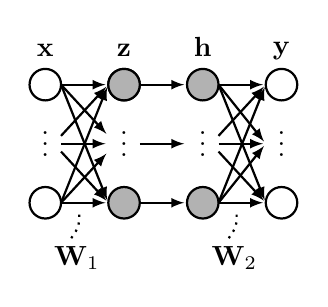
\begin{tikzpicture}[>=spaced latex]
\draw [thick] (0,-0.75) circle [radius=0.2] node[label={$\mathbf{x}$}] at (0,0.85) {};
\draw [thick] (0,0.1) node {$\vdots$};
\draw [thick] (0,0.75) circle [radius=0.2];

\draw [thick,dotted] (0.33,-1.2)  .. controls (0.43,-1.05) .. (0.43,-0.9);
\draw (0.4,-1.45) node {$\mathbf{W}_1$};

\draw [thick] [nn_edge] (0.2,-0.75) -- (0.8,-0.1);
\draw [thick] [nn_edge] (0.2,-0.75) -- (0.8,-0.75);
\draw [thick] [nn_edge] (0.2,-0.75) -- (0.8,0.75);
\draw [thick] [nn_edge] (0.2,-0.1) -- (0.8,-0.75);
\draw [thick] [nn_edge] (0.2,0.0) -- (0.8,0.0);
\draw [thick] [nn_edge] (0.2,0.1) -- (0.8,0.75);
\draw [thick] [nn_edge] (0.2,0.75) -- (0.8,0.75);
\draw [thick] [nn_edge] (0.2,0.75) -- (0.8,-0.75);
\draw [thick] [nn_edge] (0.2,0.75) -- (0.8,0.1);
\draw [thick, fill=gray_neuron] (1,0.75) circle [radius=0.2]  node[label={$\mathbf{z}$}] at (1.0,0.85) {};
\draw [thick] (1,0.1) node {$\vdots$};
\draw [thick, fill=gray_neuron] (1,-0.75) circle [radius=0.2];
\draw [thick] [nn_edge] (1.2,0.75) -- (1.8,0.75);
\draw [thick] [nn_edge] (1.2,0.0) -- (1.8,0.0);
\draw [thick] [nn_edge] (1.2,-0.75) -- (1.8,-0.75);
\draw [thick, fill=gray_neuron] (1,0.75) circle [radius=0.2]  node[label={$\mathbf{h}$}] at (2.0,0.85) {};
\draw [thick, fill=gray_neuron] (2.0,0.75) circle [radius=0.2];
\draw [thick] (2.0,0.1) node {$\vdots$};
\draw [thick, fill=gray_neuron] (2.0,-0.75) circle [radius=0.2];

\draw [thick,dotted] (2.33,-1.2)  .. controls (2.43,-1.05) .. (2.43,-0.9);
\draw (2.4,-1.45) node {$\mathbf{W}_2$};

\draw [thick] [nn_edge] (2.2,-0.75) -- (2.8,-0.75);
\draw [thick] [nn_edge] (2.2,-0.75) -- (2.8,0.75);
\draw [thick] [nn_edge] (2.2,-0.75) -- (2.8,0.0);
\draw [thick] [nn_edge] (2.2,-0.1) -- (2.8,-0.75);
\draw [thick] [nn_edge] (2.2,0.0) -- (2.8,0.0);
\draw [thick] [nn_edge] (2.2,0.1) -- (2.8,0.75);
\draw [thick] [nn_edge] (2.2,0.75) -- (2.8,0.75);
\draw [thick] [nn_edge] (2.2,0.75) -- (2.8,-0.75);
\draw [thick] [nn_edge] (2.2,0.75) -- (2.8,0.0);
\draw [thick] (3.0,-0.75) circle [radius=0.2] node[label={$\mathbf{y}$}] at (3.0,0.8) {};
\draw [thick] (3.0,0.1)  node {$\vdots$};
\draw [thick] (3.0,0.75) circle [radius=0.2];
\end{tikzpicture}
\end{minipage}
%
%
\begin{minipage}{0.77\textwidth}
\centering
\def\layerwidth{1.3}
\begin{tikzpicture}[
cblock/.style={
draw,
fill=comp_graph_node_bcolor,
rectangle, 
inner sep=1.5mm,
minimum width=\layerwidth*0.9 cm,
minimum height=\layerwidth*0.5*0.9 cm,
font=\footnotesize}]
%
\draw [thick] [comp_graph_edge] (\layerwidth*0.5,0) -- (\layerwidth,0);
%\draw (0,0) rectangle ++(1,1);
\draw (\layerwidth*1.5,0) node [cblock] {\texttt{linear}};
\draw [thick] [comp_graph_edge] (\layerwidth*2,0) -- (\layerwidth*3,0);
\draw (\layerwidth*3.5,0) node [cblock] {\texttt{relu}};
\draw [thick] [comp_graph_edge] (\layerwidth*4,0) -- (\layerwidth*5,0);
\draw (\layerwidth*5.5,0) node [cblock] {\texttt{linear}};
\draw [thick] [comp_graph_edge] (\layerwidth*6,0) -- (\layerwidth*6.25,0);

\draw (\layerwidth*0.5,0) node [fill=comp_graph_data_bcolor] {$\mathbf{x}$};
\draw (\layerwidth*2.5,0) node [fill=comp_graph_data_bcolor] {$\mathbf{z}$};
\draw (\layerwidth*4.5,0) node [fill=comp_graph_data_bcolor] {$\mathbf{h}$};
\draw (\layerwidth*6.5,0) node [fill=comp_graph_data_bcolor] {$\hat{\mathbf{y}}$};

\draw (-1,0) node {$\iff$};
\end{tikzpicture}
\end{minipage}
\caption{In this chapter we will visualize neural nets as a sequence of layers, which we call a computation graph.}
\label{fig:backpropagation:simple_MLP}
\end{figure}
\vspace{-0.2cm}

Each {\setlength{\fboxsep}{2pt}\colorbox{comp_graph_node_bcolor}{layer}} takes in some inputs and transforms them into some outputs. We call this the $\texttt{forward}$ pass through the layer. If the layer has parameters, we will consider the parameters to be an \textit{input} to a parameter-free transformation:
\begin{align}
    \xout &= f(\xin,\theta)
\end{align}
Graphically, we will depict the forward operation of a layer like shown below (\fig{\ref{fig:backpropagation:mod_block_forward}}).
\vspace{-0.2cm}
\begin{figure}[h]
\centerline{
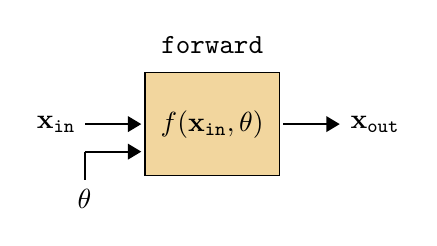
\begin{tikzpicture}%[>=spaced latex]
%
\def\layerwidth{1.8}
%
\draw [thick] [comp_graph_edge] (\layerwidth*0.6,-0.35) -- (\layerwidth,-0.35);
\draw [thick] (\layerwidth*0.6,-0.75) -- (\layerwidth*0.6,-0.35);
\draw [thick] [comp_graph_edge] (\layerwidth*0.5,0) -- (\layerwidth,0);
\draw (\layerwidth*1.5,0) node [fill=comp_graph_node_bcolor,draw, inner sep=2mm, minimum height=1.3cm] {$f(\xin, \theta)$};
\draw [thick] [comp_graph_edge] (\layerwidth*2,0) -- (\layerwidth*2.4,0);
%
\draw (\layerwidth*0.6,-0.95) node [fill=white] {$\theta$};
\draw (\layerwidth*0.4,0) node [fill=comp_graph_data_bcolor] {$\xin$};
\draw (\layerwidth*2.65,0) node [fill=comp_graph_data_bcolor] {$\xout$};
\draw (\layerwidth*1.5,1) node {\texttt{forward}};
%
\end{tikzpicture}
}
\caption{Forward operation of a neural net layer.}
\label{fig:backpropagation:mod_block_forward}
\end{figure}
\vspace{-0.2cm}

% \begin{figure}[h]
% \centering
% \begin{tikzpicture}%[>=spaced latex]
% %
% \def\layerheight{1.0}

% \draw [thick] [comp_graph_edge] (0,0) -- (0,\layerheight);
% %\draw (0,0) rectangle ++(1,1);
% \draw (0,\layerheight*1.5) node [fill=comp_graph_node_bcolor,draw, inner sep=2mm] {$f(\xin)$};
% \draw [thick] [comp_graph_edge] (0,\layerheight*2) -- (0,\layerheight*3);

% \draw (0,\layerheight*0.4) node [fill=comp_graph_data_bcolor] {$\xin$};
% \draw (0,\layerheight*2.4) node [fill=comp_graph_data_bcolor] {$\xout$};

% \end{tikzpicture}
% \label{fig:backpropagation:mod_block}
% \end{figure}

% \begin{figure}[h]
%     \centering
%     \includegraphics[width=0.18\linewidth]{./figures/backpropagation/mod_block.pdf}
%     \label{fig:mod_block}
% \end{figure}

%A graph of computational blocks like this is called a \textbf{computation graph}.

The learning problem is to find the parameters {\setlength{\fboxsep}{2pt}\colorbox{comp_graph_param_bcolor}{$\theta$}} that achieve a desired mapping. Usually we will solve this problem via gradient descent. The question of this chapter is, how do we compute the gradients?
\marginnote{We will use the color \raisebox{1mm}{\colorbox{comp_graph_param_bcolor}{\makebox(0,0){}}} to indicate \textit{free} parameters, which are set via learning and are not the result of any other processing.}[-1.9cm]
%These parameters, along with the input training data, are the leaves in the computation graph.

\textbf{Backpropagation} is an algorithm that efficiently calculates the gradient of the loss with respect to each and every parameter in a computation graph. It relies on a special new operation, called \texttt{backward} that, just like \texttt{forward}, can be defined for each layer, and acts in isolation from the rest of the graph. But first, before we get to defining \texttt{backward}, we will build up some intuition about the key trick backpropagation will exploit.

\section{The Trick of Backpropagation: Reuse of Computation}

To start, we will consider a simple computation graph that is a chain of functions $f_L \circ f_{L-1} \circ \cdots f_2 \circ f_1$, with each function $f_l$ parameterized by $\theta_l$.\marginnote{Such a computation graph could represent an MLP, for example, which we will see in the next section.}[-0.4cm] We aim to optimize the parameters with respect to a loss function $\mathcal{L}$. The loss can be treated as another node in our computation graph, which takes in $\mathbf{x}_L$ (the output of $f_L$) and outputs a scalar $J$, the loss. This computation graph appears as follows (\fig{\ref{fig:backpropagation:composed_modules}}).
\begin{figure}[h]
    \centerline{
    \def\layerwidth{1.2}
    \begin{tikzpicture}[
    cblock/.style={
    draw,
    fill=comp_graph_node_bcolor,
    rectangle, 
    inner sep=1.5mm,
    minimum width=\layerwidth*0.9 cm,
    minimum height=\layerwidth*0.75*0.9 cm}]
    %
    %
    % draw f nodes
    \def\fnames {{"$f_0$","$f_1$","$f_2$","$f_{L-1}$","$f_L$"}}
    \foreach \x in {1,2,3,4} {
        \pgfmathparse{\fnames[\x]};
        \draw ($(\layerwidth*2*\x-\layerwidth+\layerwidth*0.5,0)$) node [cblock] {\pgfmathresult};
    }
    % draw data arrows
    \draw [thick] [comp_graph_edge] (\layerwidth*0.5,0) -- (\layerwidth,0);
    \foreach \x in {1,2,3,4} {
        % data arrow
        \draw [thick] [comp_graph_edge] (\layerwidth*2*\x,0) -- (\layerwidth*2*\x+\layerwidth,0);
    }
    \draw [thick] [comp_graph_edge] (\layerwidth*10,0) -- (\layerwidth*10.25,0);
    %
    % draw param arrows
    \foreach \x in {0,1,2,3} {
        \draw [thick] [comp_graph_edge] (\layerwidth*2*\x+\layerwidth*0.6,-0.35) -- (\layerwidth*2*\x+\layerwidth,-0.35);
        \draw [thick] (\layerwidth*2*\x+\layerwidth*0.6,-0.75) -- (\layerwidth*2*\x+\layerwidth*0.6,-0.35);
    }
    %
    % draw data and params
    \def\datanames {{"$\mathbf{x}_0$","$\mathbf{x}_1$","$\cdots$","$\mathbf{x}_{L-1}$","$\mathbf{x}_L$"}}
    \def\paramnames {{"$\theta_1$","$\theta_2$","$\theta_{L-1}$","$\theta_{L}$"}}
    \foreach \x in {0,1,2,3,4} {
        \pgfmathparse{\datanames[\x]};
        \draw ($(\layerwidth*2*\x+\layerwidth*0.5,0)$) node [fill=comp_graph_data_bcolor] {\pgfmathresult};
        %
    };
    \foreach \x in {0,1,2,3} {
        \pgfmathparse{\paramnames[\x]};
        \draw ($(\layerwidth*2*\x+\layerwidth*0.5,-0.95)$) node [fill=comp_graph_param_bcolor] {\pgfmathresult};
    };
    %
    % loss node
    \draw (\layerwidth*9.5,0) node [cblock, fill=comp_graph_loss_node_bcolor] {$\mathcal{L}$};
    \draw (\layerwidth*10.4,0) node [fill=comp_graph_data_bcolor] {$J$};
    %
    \draw (6.3,-1.4) node {$\underbrace{\quad\quad\quad\quad\quad\quad\quad\quad\quad\quad\quad\quad\quad\quad\quad\quad\quad\quad\quad\quad\quad\quad\quad\quad\quad\quad\quad\quad\quad\quad\quad\quad\quad\quad\quad}$};
    \draw (6.3,-1.9) node [scale=1.25] {$\frac{\partial J}{\partial \theta_1}$};
    \draw (7.6,-2.4) node {$\underbrace{\quad\quad\quad\quad\quad\quad\quad\quad\quad\quad\quad\quad\quad\quad\quad\quad\quad\quad\quad\quad\quad\quad\quad\quad\quad\quad\quad\quad}$};
    \draw (7.6,-2.9) node [scale=1.25] {$\frac{\partial J}{\partial \theta_2}$};
    %
    \end{tikzpicture}
    }
    \caption{Basic sequential computation graph.}
    \label{fig:backpropagation:composed_modules}
\end{figure}
\marginnote{This computation graph is a narrow tree; the parameters live on branches of length 1. This can be easier to see when we plot it with data and parameters as nodes and edges as the functions:
\medbreak
\centerline{
\includegraphics[width=0.45\linewidth]{./figures/backpropagation/cgraph_tree.pdf}
}
The parameters, along with the input training data, are the leaves of the computation graph.
}[2.4cm]

Our goal is to update all the values highlighted in blue: $\theta_1$, $\theta_2$, and so forth. To do so we need to compute the gradients $\frac{\partial J}{\partial \theta_1}$, $\frac{\partial J}{\partial \theta_2}$, etc. Each of these gradients can be calculated via the chain rule. Here is the chain rule written out for the gradients for $\theta_1$ and $\theta_2$:
\begin{align}
    \frac{\partial J}{\partial \theta_1} &= \highlight[shared_term_color]{\frac{\partial J}{\partial \mathbf{x}_L}\frac{\partial \mathbf{x}_L}{\partial \mathbf{x}_{L-1}} \cdots \frac{\partial \mathbf{x}_3}{\partial \mathbf{x}_2}} \frac{\partial \mathbf{x}_2}{\mathbf{x}_1}\frac{\partial \mathbf{x}_1}{\partial \mathbf{\theta}_1}\\
    \frac{\partial J}{\partial \theta_2} &=  \highlight[shared_term_color]{\frac{\partial J}{\partial \mathbf{x}_{L}}\frac{\partial \mathbf{x}_L}{\partial \mathbf{x}_{L-1}} \cdots \frac{\partial \mathbf{x}_3}{\partial \mathbf{x}_2}} \frac{\partial \mathbf{x}_2}{\partial \theta_2}
\end{align}
Rather than evaluating both equations separately, we notice that all the terms in each gray box are shared. We only need to evaluate this product once, and then can use it to compute both $\frac{\partial J}{\partial \theta_1}$ and $\frac{\partial J}{\partial \theta_2}$. Now notice that this pattern of reuse can be applied in the same way for $\theta_3$, $\theta_4$, and so on. This is the whole trick of backpropagation: rather than computing each layer's gradients independently, observe that they share many of the same terms, so we might as well calculate each shared term once and reuse them. \marginnote{This strategy, in general, is called {\bf dynamic programming}.}[-0.6cm]

%\section{\texttt{Backward} for a generic layer}
\section{Backward for a Generic Layer}
To come up with a general algorithm for reusing all the shared computation, we will first look at one generic layer in isolation, and see what we need in order to update its parameters (\fig{\ref{fig:backpropagation:generic_layer_g_L}}).
\begin{figure}[h]
\centerline{
\begin{tikzpicture}%[>=spaced latex]
%
\def\layerwidth{1.8}
%
\draw [thick] [comp_graph_edge] (\layerwidth*0.6,-0.35) -- (\layerwidth,-0.35);
\draw [thick] (\layerwidth*0.6,-0.75) -- (\layerwidth*0.6,-0.35);
\draw [thick] [comp_graph_edge] (\layerwidth*0.5,0) -- (\layerwidth,0);
\draw (\layerwidth*1.5,0) node [fill=comp_graph_node_bcolor,draw, inner sep=2mm, minimum height=1.3cm] {$f(\xin, \theta)$};
\draw [thick] [comp_graph_edge] (\layerwidth*2,0) -- (\layerwidth*2.4,0);
%
\draw (\layerwidth*0.6,-0.95) node [fill=comp_graph_param_bcolor] {$\theta$};
\draw (\layerwidth*0.4,0) node [fill=comp_graph_data_bcolor] {$\xin$};
\draw (\layerwidth*2.65,0) node [fill=comp_graph_data_bcolor] {$\xout$};
\draw (\layerwidth*3,0) node {$\cdots$};
\draw [thick] [comp_graph_edge] (\layerwidth*3.2,0) -- (\layerwidth*3.6,0);
\draw (\layerwidth*3.8,0) node {$J$};
\draw [thick] [comp_graph_edge] (-0.2*\layerwidth,0) -- (0.2*\layerwidth,0);
\draw (-0.4*\layerwidth,0) node {$\cdots$};
%
\draw (2.8,-1.4) node {$\underbrace{\quad\quad\quad\quad\quad\quad\quad\quad\quad\quad\quad\quad\quad}$};
\draw (2.8,-1.9) node [scale=1.2] {$\localgrad$};
\draw (5.8,-1.8) node {$\underbrace{\quad\quad\quad\quad\quad\quad\quad}$};
\draw (5.8,-2.3) node [scale=1.2] {$\costgradout$};
\draw (3.8,-2.6) node {$\underbrace{\quad\quad\quad\quad\quad\quad\quad\quad\quad\quad\quad\quad\quad\quad\quad\quad\quad\quad\quad}$};
\draw (3.8,-3.1) node [scale=1.2] {$\costgradin$};
%
\end{tikzpicture}
}
\caption{A generic layer in the computation graph. The braces represent the part of the computation graph we need to consider in order to evaluate $\costgradout$, $\localgrad$, and $\costgradin$.}
\label{fig:backpropagation:generic_layer_g_L}
\end{figure}

% Here we have introduced two new shorthands, $\localgrad$ and $\costgrad$ -- these represent arrays of partial derivatives, defined below, and they are the key arrays we need to keep track of to do backprop. They are defined as:
% %To update $\theta$ for this layer, we just need to know $\frac{\partial J}{\partial \theta}$
% %This strategy involves two key matrices: 1) the vector of derivatives of the cost $J$ w.r.t to each layer's inputs, and 2) the matrix of derivatives of the outputs of each layer with respect to its inputs. We define shorthand for these below:
% \marginnote{All these arrays represent the gradient \textit{at a single operating point} --  that of the current value of the data and parameters.}[1cm]
% \begin{align}
%     \costgrad &\triangleq \frac{\partial J}{\partial [\xin, \xout, \theta]} &&\quad\quad \triangleleft \quad \text{grad of cost}\\
%      &\quad\quad \costgradxin \triangleq \frac{\partial J}{\partial \xin} &&\quad\quad \triangleleft \quad \text{... w.r.t. layer inputs} \quad [1 \times |\xin|]\\
%      &\quad\quad \costgradxout \triangleq \frac{\partial J}{\partial \xout} &&\quad\quad \triangleleft \quad \text{... w.r.t. layer outputs} \quad [1 \times |\xout|]\\
%      &\quad\quad \costgradtheta \triangleq \frac{\partial J}{\partial \theta} &&\quad\quad \triangleleft \quad \text{... w.r.t. layer params} \quad [1 \times |\theta|]\\
%     \localgrad &\triangleq \frac{\partial \xout}{\partial [\xin, \theta]} &&\quad\quad \triangleleft \quad \text{grad of layer}\\
%     &\quad\quad \localgradx \triangleq \frac{\partial \xout}{\partial \xin} &&\quad\quad \triangleleft \quad \text{... w.r.t. layer input data} \quad [|\xout| \times |\xin|]\\
%     &\quad\quad \localgradtheta \triangleq \frac{\partial \xout}{\partial \theta} &&\quad\quad \triangleleft \quad \text{... w.r.t. layer params} \quad [|\xout| \times |\theta|]
%     %\mathbf{F}_l &\triangleq \frac{\partial \mathbf{x}_{l}}{\partial \mathbf{x}_{l-1}} = \frac{\partial f_l(\mathbf{x}_{l-1})}{\partial \mathbf{x}_{l-1}} &\quad\quad \triangleleft \quad [N \times M]
% \end{align}

% Computing $\localgrad$ is an entirely local process: for each layer, we just need to know the functional form of its derivative, $f^{\prime}$, which we then evaluate at the operating point $[\xin, \theta]$ to obtain $\localgrad = f^{\prime}(\xin,\theta)$.

% Computing $\costgrad$ is a bit trickier; it requires evaluating the chain rule, and depends on all the subsequent layers of processing, that come between the current layer and $J$. However, this can be computed iteratively: once we know $\costgrad_l$, for some layer $l$, computing $\costgrad_{l-1}$ is just one more matrix multiply! This can be summarized with the following recurrence relation:
% \begin{align}
%     \costgrad_{\texttt{in}} &= \costgrad_{\texttt{out}}\localgrad^{\mathbf{x}} &&\quad\quad \triangleleft \quad \text{``backpropagation of errors"} \label{eqn:backpropagation:backward}
% \end{align}
% This recurrence is essence of backprop: it sends ``error signals" (gradients) backwards through the network, starting at the last layer and iteratively applying Equation \ref{eqn:backpropagation:backward} to
% compute $\costgrad$ for each previous layer.
% \marginnote{Deep learning libraries like Pytorch have a \texttt{.grad} field associated with each variable (data, activations, parameters). This field reprsents $\frac{\partial J}{\partial v}$ for each variable $v$.}[-0.4cm]

% To do gradient-based learning, we need to compute the gradient of the cost w.r.t. the parameters, i.e. $\costgradtheta$. This gives us the parameter \texttt{update} step in gradient descent: 
% \begin{align}
%     \theta^{i+1} &\leftarrow \theta^{i} - \eta (\costgradtheta)^T &&\quad\quad \triangleleft \quad \texttt{update} \label{eqn:backpropagation:djdtheta}
% \end{align}
% \marginnote{The transpose is because, by convention $\theta$ is a column vector while $\costgradtheta = \frac{\partial J}{\partial \theta}$ is a row vector; see Appendix.}[-0.4cm]

% %These arrays give a simple formula for computing the gradient we need -- $\frac{\partial J}{\partial \theta}$ -- in order to \texttt{update} $\theta$ to minimize the cost:
% %\begin{align}
% %    \frac{\partial J}{\partial \theta_l} = \costgrad_l\localgrad^{\theta}_l \quad\quad \triangleleft \quad [1 \times |\xout|]\cdot[|\xout| \times |\theta|] \rightarrow [1 \times \theta]] \label{eqn:backpropagation:param_update}
% %\end{align}

% %The remaining question is just: how do we get $\costgrad_l$ and $\localgrad^{\theta}_l$ for layer $l$? 

% Now, observe that if we already knew $\costgradxout$, then computing $\costgradtheta$ would be easy, it would just be the following matrix product:
% \begin{align}
%     \costgradtheta = \frac{\partial J}{\partial \theta} = \frac{\partial J}{\partial \xout} \frac{\partial \xout}{\partial \theta} = \costgradxout \localgradtheta
% \end{align}

Here we have introduced two new shorthands, $\localgrad$ and $\costgrad$; these represent arrays of partial derivatives, defined below, and they are the key arrays we need to keep track of to do backprop. They are defined as:
%To update $\theta$ for this layer, we just need to know $\frac{\partial J}{\partial \theta}$
%This strategy involves two key matrices: 1) the vector of derivatives of the cost $J$ w.r.t to each layer's inputs, and 2) the matrix of derivatives of the outputs of each layer with respect to its inputs. We define shorthand for these below:
\marginnote{All these arrays represent the gradient \textit{at a single operating point}, namely that of the current value of the data and parameters.}[0.9cm]
\begin{align}
    %\costgrad &\triangleq \frac{\partial J}{\partial [\xin, \xout]} &&\quad\quad \triangleleft \quad \text{grad of cost}\\
    % &\quad\quad \costgradin \triangleq \frac{\partial J}{\partial \xin} &&\quad\quad \triangleleft \quad \text{... w.r.t. layer input data} \quad [1 \times |\xin|]\\
    % &\quad\quad \costgradout \triangleq \frac{\partial J}{\partial \xout} &&\quad\quad \triangleleft \quad \text{... w.r.t. layer outputs} \quad [1 \times |\xout|]\\
    \costgradl &\triangleq \frac{\partial J}{\partial \mathbf{x}_l} &&\quad\quad \triangleleft \quad \text{grad of cost with respect to } \mathbf{x}_l \quad [1 \times |\mathbf{x}_l|]\\
    \localgrad &\triangleq \frac{\partial \xout}{\partial [\xin, \theta]} &&\quad\quad \triangleleft \quad \text{grad of layer}\\
    &\quad\quad \localgrad^{\mathbf{x}} \triangleq \frac{\partial \xout}{\partial \xin} &&\quad\quad \triangleleft \quad \text{\quad with respect to layer input data} \quad [|\xout| \times |\xin|]\\
    &\quad\quad \localgrad^{\theta} \triangleq \frac{\partial \xout}{\partial \theta} &&\quad\quad \triangleleft \quad \text{\quad with respect to layer params} \quad [|\xout| \times |\theta|]
    %\mathbf{F}_l &\triangleq \frac{\partial \mathbf{x}_{l}}{\partial \mathbf{x}_{l-1}} = \frac{\partial f_l(\mathbf{x}_{l-1})}{\partial \mathbf{x}_{l-1}} &\quad\quad \triangleleft \quad [N \times M]
\end{align}

These arrays give a simple formula for computing the gradient we need, that is, $\frac{\partial J}{\partial \theta}$, in order to \texttt{update} $\theta$ to minimize the cost:
%\begin{align}
%    \frac{\partial J}{\partial \theta_l} = \costgrad_l\localgrad^{\theta}_l \quad\quad \triangleleft \quad [1 \times |\xout|]\cdot[|\xout| \times |\theta|] \rightarrow [1 \times \theta]] \label{eqn:backpropagation:param_update}
%\end{align}
\begin{align}
    \frac{\partial J}{\partial \theta} &= \underbrace{\frac{\partial J}{\partial \xout}}_{\costgradout} \underbrace{\frac{\partial \xout}{\partial \theta}}_{\localgradtheta} = \costgradout\localgradtheta\\
    \theta^{i+1} &\leftarrow \theta^{i} - \eta \Big(\frac{\partial J}{\partial \theta}\Big)^\transpose &&\quad\quad \triangleleft \quad \texttt{update} \label{eqn:backpropagation:djdtheta}
\end{align}
\marginnote{The transpose is because, by convention, $\theta$ is a column vector while $\frac{\partial J}{\partial \theta}$ is a row vector; see the Notation section prior to chapter 1.}[-0.5cm]

The remaining question is clear: how do we get $\costgrad_l$ and $\localgrad^{\theta}_l$ for each layer $l$? 

Computing $\localgrad$ is an entirely local process: for each layer, we just need to know the functional form of its derivative, $f^{\prime}$, which we then evaluate at the operating point $[\xin, \theta]$ to obtain $\localgrad = f^{\prime}(\xin,\theta)$.

Computing $\costgrad$ is a bit trickier; it requires evaluating the chain rule, and depends on all the layers between $\xout$ and $J$. However, this can be computed iteratively: once we know $\costgrad_l$, computing $\costgrad_{l-1}$ is just one more matrix multiply! This can be summarized with the following recurrence relation:
\begin{align}
    \costgrad_{\texttt{in}} &= \costgrad_{\texttt{out}}\localgrad^{\mathbf{x}} &&\quad\quad \triangleleft \quad \text{backpropagation of errors}
    \label{eqn:backpropagation:backward}
\end{align}
This recurrence is essence of backprop: it sends error signals (gradients) backward through the network, starting at the last layer and iteratively applying \eqn{\ref{eqn:backpropagation:backward}} to
compute $\costgrad$ for each previous layer.
\marginnote{Deep learning libraries like Pytorch have a \texttt{.grad} field associated with each variable (data, activations, parameters). This field represents $\frac{\partial J}{\partial v}$ for each variable $v$.}[-0.8cm]


We are finally ready to define the full \texttt{backward} function promised at the beginning of this chapter! It consists of the following operation, shown in \fig{\ref{fig:backpropagation:mod_block_backward}}, which has three inputs ($\xin, \theta, \costgrad_{\texttt{out}}$) and two outputs ($\costgrad_{\texttt{in}}$ and $\frac{\partial J}{\partial \theta}$).
\begin{figure}[h]
\centerline{
\begin{tikzpicture}%[>=spaced latex]
%
\def\layerwidth{1.8}
%
\draw [thick] [comp_graph_edge] (0.4,0.6) -- (\layerwidth*0.6,0.6);
\draw [thick] [comp_graph_edge] (\layerwidth*0.6,0) -- (0.4,0);
\draw [thick] [comp_graph_edge] (0.5,-0.6) -- (0.5,-0.95);
\draw [thick] (\layerwidth*0.6,-0.6) -- (0.5,-0.6);
\draw (\layerwidth*1.5,0) node [fill=comp_graph_node_bcolor,draw, inner sep=2mm, minimum height=1.8cm, minimum width=3.0cm] {};
\draw (\layerwidth*1.5,1.2) node {\texttt{backward}};
\draw (\layerwidth*1.5,0.6) node  {$\localgrad = f^{\prime}(\xin,\theta)$};
\draw (\layerwidth*1.5,0) node  {$\costgrad_{\texttt{in}} = \costgrad_{\texttt{out}}\localgrad^{\mathbf{x}}$};
\draw (\layerwidth*1.5,-0.6) node  {$\frac{\partial J}{\partial \theta} = \costgrad_{\texttt{out}}\localgrad^{\theta}$};
\draw [thick] [comp_graph_edge] (\layerwidth*2.8,0) -- (\layerwidth*2.4,0);
%
\draw (0.5,-1.3) node [fill=comp_graph_param_grad_bcolor] {$\frac{\partial J}{\partial \theta}$};
\draw (-0.2,0.6) node [fill=comp_graph_data_bcolor] {$\xin, \theta$};
\draw (0,0) node [fill=comp_graph_data_bcolor] {$\costgrad_{\texttt{in}}$};
\draw (\layerwidth*3,0) node [fill=comp_graph_data_bcolor] {$\costgrad_{\texttt{out}}$};
%
\end{tikzpicture}
}
\caption{\texttt{backward} for a generic layer. We use the color \raisebox{1mm}{\colorbox{comp_graph_param_grad_bcolor}{\makebox(0,0){}}} to indicate parameter gradients.}
\label{fig:backpropagation:mod_block_backward}
\end{figure}

% For any $\frac{\partial J}{\partial \theta_l}$, we have:
% \begin{align}
%     \frac{\partial J}{\partial \theta_l} = \frac{\partial J}{\partial \mathbf{x}_l}\frac{\partial \mathbf{x}_l}{\partial \theta_l}
% \end{align}
% This says that all the parameter updates can be computed with just one further matrix multiply once we know $\frac{\partial J}{\partial \mathbf{x}_l}$ for all $l$. Now, the trick is to work backwards to compute all the $\frac{\partial J}{\partial \mathbf{x}_l}$, because:
% \begin{align}
%     \frac{\partial J}{\partial \mathbf{x}_l} = \frac{\partial J}{\partial \mathbf{x}_{l+1}}\frac{\partial \mathbf{x}_{l+1}}{\partial \mathbf{x}_l}
% \end{align}
% So, once we know $\frac{\partial J}{\partial \mathbf{x}_{l+1}}$ we can compute $\frac{\partial J}{\partial \mathbf{x}_{l}}$ with just one additional matrix multiply.

%The value of the blue terms is $\frac{\partial j}{\partial \mathbf{x}_2}$. Once we have calculated this value, we can 

%Indeed, once we've computed $\frac{\partial \mathbf{x}_{L}}{\partial \mathbf{x}_{l}}$, we can compute $\frac{\partial \mathbf{x}_{L}}{\partial \mathbf{x}_{l-1}}$ with just one more multiply:
%\begin{align}
%    \frac{\partial \mathbf{x}_{L}}{\partial \mathbf{x}_{l-1}} = \frac{\partial \mathbf{x}_{L}}{\partial \mathbf{x}_{l}} \frac{\partial \mathbf{x}_{l}}{\partial \mathbf{x}_{l-1}}
%\end{align}

%\section{Backprop through chains}


% \begin{align}
%     \xout &= f(\xin,\theta) &&\quad\quad \triangleleft \quad \texttt{forward}\\
%     \costgrad_{\texttt{in}} &= \costgrad_{\texttt{out}}\localgrad^{\mathbf{x}} &&\quad\quad \triangleleft \quad \texttt{backward}
% \end{align}

% And then update parameters:
% \begin{align}
%     \frac{\partial J}{\partial \theta} &= \costgrad_{\texttt{out}}\localgrad^{\theta} &&\quad\quad \triangleleft \quad \texttt{update}
% \end{align}


\section{The Full Algorithm: Forward, Then Backward}
We are ready now to define the full backprop algorithm. In the last section we saw that we can easily compute the gradient update for $\theta_l$ once we have computed $\localgrad_l$ and $\costgrad_l$.\marginnote{The $\costgrad_l$ and $\localgrad_l$ are the $\costgrad$ and $\localgrad$ arrays for layer $l$.}[-0.0cm]

So, we just need to order our operations so that when we get to updating layer $l$ we have these two arrays ready. The way to do it is to first compute a \textbf{forward pass} through the entire network, which means starting with input data $\mathbf{x}_0$ and evaluating layer by layer to produce the sequence $\mathbf{x}_0, \mathbf{x}_1, \ldots, \mathbf{x}_L$. \Fig{\ref{fig:backpropagation:forward_pass}} shows what the forward pass looks like.
\begin{figure}[h]
    \centerline{
    \def\layerwidth{1.3}
    \begin{tikzpicture}[
    cblock/.style={
    draw,
    fill=comp_graph_node_bcolor,
    rectangle, 
    inner sep=1.5mm,
    minimum width=\layerwidth*0.9 cm,
    minimum height=\layerwidth*0.75*0.9 cm}]
    %
    %
    % draw f nodes
    \def\fnames {{"$f_0$","$f_1$","$f_2$","$f_{L-1}$","$f_L$"}}
    \foreach \x in {1,2,3,4} {
        \pgfmathparse{\fnames[\x]};
        \draw ($(\layerwidth*2*\x-\layerwidth+\layerwidth*0.5,0)$) node [cblock] {\pgfmathresult};
    }
    % draw data arrows
    \draw [thick] [comp_graph_edge_forward] (\layerwidth*0.5,0) -- (\layerwidth,0);
    \foreach \x in {1,2,3,4} {
        % data arrow
        \draw [thick] [comp_graph_edge_forward] (\layerwidth*2*\x,0) -- (\layerwidth*2*\x+\layerwidth,0);
    }
    %\draw [thick] [comp_graph_edge_forward] (\layerwidth*10,0) -- (\layerwidth*10.25,0);
    %
    % draw param arrows
    \foreach \x in {0,1,2,3} {
        \draw [thick] [comp_graph_edge_forward] (\layerwidth*2*\x+\layerwidth*0.6,-0.35) -- (\layerwidth*2*\x+\layerwidth,-0.35);
    }
    %
    % draw data and params
    \def\datanames {{"$\mathbf{x}_0$","$\mathbf{x}_1$","$\cdots$","$\mathbf{x}_{L-1}$","$\mathbf{x}_L$"}}
    \def\paramnames {{"$\theta_1$","$\theta_2$","$\theta_{L-1}$","$\theta_{L}$"}}
    \foreach \x in {0,1,2,3,4} {
        \pgfmathparse{\datanames[\x]};
        \draw ($(\layerwidth*2*\x+\layerwidth*0.5,0)$) node [fill=white] {\pgfmathresult};
        %
    };
    \foreach \x in {0,1,2,3} {
        \pgfmathparse{\paramnames[\x]};
        \draw ($(\layerwidth*2*\x+\layerwidth*0.5,-0.4)$) node [fill=white] {\pgfmathresult};
    };
    %
    % loss node
    \draw (\layerwidth*9.5,0) node [cblock, fill=comp_graph_loss_node_bcolor] {$\mathcal{L}$};
    %\draw (\layerwidth*10.4,0) node [fill=comp_graph_data_bcolor] {$J$};
    %
    %\draw (\layerwidth*5.5,1.0) node {\textbf{Forward pass}};
    %
    \end{tikzpicture}
    }
    \caption{Forward pass.}
    \label{fig:backpropagation:forward_pass}
\end{figure}
\marginnote{We use the color \raisebox{1mm}{\colorbox{forwardpropcolor}{\makebox(0,0){}}} for data/activations being passed forward through the network.}[2.0cm]

%We need this sequence because, in general, $\localgrad$ for a layer will be a function of $\xin$ and $\theta$ for that layer -- so we need the full sequence of inputs and outputs to each layer to get compute the full sequence $\localgrad_1, \localgrad_2, \ldots$. 

Next, we compute a \textbf{backward pass}, iteratively evaluating the $\costgrad$'s and obtaining the sequence $\costgrad_L, \costgrad_{L-1}, \ldots$, as well as the parameter gradients for each layer (\fig{\ref{fig:backpropagation:backward_pass}}). %Remember that to compute $\costgrad$ for a layer, we need $\localgrad$ for that layer, so on the
\begin{figure}[h]
    \centerline{
    \def\layerwidth{1.3}
    \begin{tikzpicture}[
    cblock/.style={
    draw,
    fill=comp_graph_node_bcolor,
    rectangle, 
    inner sep=1.5mm,
    minimum width=\layerwidth*0.9 cm,
    minimum height=\layerwidth*0.75*0.9 cm}]
    %
    %
    % draw f nodes
    \def\fnames {{"$f^{\prime}_0$","$f^{\prime}_1$","$f^{\prime}_2$","$f^{\prime}_{L-1}$","$f^{\prime}_L$"}}
    \foreach \x in {1,2,3,4} {
        \pgfmathparse{\fnames[\x]};
        \draw ($(\layerwidth*2*\x-\layerwidth+\layerwidth*0.5,0)$) node [cblock] {\pgfmathresult};
    }
    % draw data arrows
    \draw [thick] [comp_graph_edge_backward] (\layerwidth,0) -- (\layerwidth*0.7,0);
    \foreach \x in {1,2,3,4} {
        % data arrow
        \draw [thick] [comp_graph_edge_backward] (\layerwidth*2*\x+\layerwidth,0) -- (\layerwidth*2*\x,0);
    }
    \draw [thick] [comp_graph_edge_backward] (\layerwidth*10.25,0) -- (\layerwidth*10,0);
    %
    % draw data and params
    \def\datanames {{"$\costgrad_0$","$\costgrad_1$","$\cdots$","$\costgrad_{L-1}$","$\costgrad_L$"}}
    \def\paramnames {{"$\frac{\partial J}{\partial \theta_1}$","$\frac{\partial J}{\partial \theta_2}$","$\frac{\partial J}{\partial \theta_{L-1}}$","$\frac{\partial J}{\partial \theta_{L}}$"}}
    \foreach \x in {0,1,2,3,4} {
        \pgfmathparse{\datanames[\x]};
        \draw ($(\layerwidth*2*\x+\layerwidth*0.5,0)$) node [fill=comp_graph_data_bcolor] {\pgfmathresult};
        %
    };
    \foreach \x in {0,1,2,3} {
        \pgfmathparse{\paramnames[\x]};
        \draw ($(\layerwidth*2*\x+\layerwidth*0.5,-0.5)$) node [fill=white] {\pgfmathresult};
    };
    % draw param arrows
    \foreach \x in {0,1,2,3} {
        \draw [thick] [comp_graph_edge_backward] (\layerwidth*2*\x+\layerwidth,-0.35) -- (\layerwidth*2*\x+\layerwidth*0.8,-0.35);
    }
    %
    % loss node
    \draw (\layerwidth*9.5,0) node [cblock, fill=comp_graph_loss_node_bcolor] {$\mathcal{L}^{\prime}$};
    \draw (\layerwidth*10.4,0) node [fill=comp_graph_data_bcolor] {$1$};
    %
    %\draw (\layerwidth*5.5,1.0) node {\textbf{Backward pass}};
    %
    \end{tikzpicture}
    }
    \caption{Backward pass.}
    \label{fig:backpropagation:backward_pass}
\end{figure}
\marginnote{We use the color \raisebox{1mm}{\colorbox{backwardpropcolor}{\makebox(0,0){}}} for data/activation gradients being passed backward through the network.}[2cm]

%Finally, we have all the arrays necessary to compute the gradients $\frac{\partial J}{\partial \theta_l}$ for all $l$ and update all the parameters in the computation graph. 
%Finally, we update our parameters based on the gradients $\frac{\partial J}{\partial \theta_l}$, and repeat. 
The full algorithm is summarized in \algref{\ref{alg:backpropagation:backprop_for_chains}}. %A graphical depiction is given in Figure \ref{fig:backpropagation:backprop_alg_diagram}.

\begin{algorithm}[h]
\SetAlgoVlined
\DontPrintSemicolon
%\marginnote{{\bf Algorithm \ref{alg:backpropagation:backprop_for_chains}}: A simple version of the backpropagation algorithm. This will work for the computation graphs we have seen so far, which consist of a series of layers, $f_1 \circ \ldots \circ f_L$, with no merging or branching (see \sect{\ref{sec:backpropagation:branch_and_merge}} for how to handle more complicated graphs with merge and branch operations).}
\caption{{\bf Algorithm \ref{alg:backpropagation:backprop_for_chains}}: Backpropagation (for chain computation graphs). A simple version of the backpropagation algorithm. This will work for the computation graphs we have seen so far, which consist of a series of layers, $f_1 \circ \ldots \circ f_L$, with no merging or branching (see \sect{\ref{sec:backpropagation:branch_and_merge}} for how to handle more complicated graphs with merge and branch operations).}
\fakealgorithmcaption{}
\label{alg:backpropagation:backprop_for_chains}
{\bf Input:} parameter vector $\theta = \{\theta_l\}_{l=1}^L$, $f_1, \ldots, f_L$, $f^{\prime}_1, \ldots, f^{\prime}_L$, training datapoint $\{\mathbf{x}_0,\mathbf{y}\}$, Loss function $\mathcal{L}: \mathbb{R}^N \rightarrow \mathbb{R}$\;
{\bf Output:} gradient direction $\frac{\partial J}{\partial \theta} = \Big\{\frac{\partial J}{\partial \theta_l}\Big\}_{l=1}^L$ \;
\;
\textbf{Forward pass:}\;
\For{\upshape $l=1, \dots, L$} {
    $\mathbf{x}_l = f_l(\mathbf{x}_{l-1}, \theta_l)$\;
}
%$J = \mathcal{L}(\mathbf{x}_L,y)$\;
\;
\textbf{Backward pass:}\;
$\costgrad_L = \mathcal{L}^{\prime}(\mathbf{x}_L,y)$\;
\For{\upshape $l=L, \dots, 1$} {
    $\localgrad_{l} = f_l^{\prime}(\mathbf{x}_{l-1},\theta_l)$\;
    $\costgrad_{l-1} = \costgrad_{l}\localgrad^{\mathbf{x}}_{l}$\;
    $\frac{\partial J}{\partial \theta_l} = \costgrad_{l}\localgrad^{\theta}_{l}$\;
}
\end{algorithm}

\section{Backpropagation Over Data Batches}
So far, we have only examined computing the gradient of the loss for a single datapoint, $\mathbf{x}$. As you may recall from \chaps{\ref{chapter:intro_to_learning}} and \ref{chapter:gradient_descent}, the total cost function we wish to minimize will typically be the \textit{average} of the losses over \textit{all} the datapoints in a training set, $\{\mathbf{x}^{(i)}\}_{i=1}^N$. However, once we know how to compute the gradient for a single datapoint, we can easily compute the gradient for the whole dataset, due to the following identity:
\begin{align}
    \frac{\partial \frac{1}{N}\sum_{i=1}^N J_i(\theta)}{\partial \theta} = \frac{1}{N} \sum_{i=1}^N \frac{\partial J_i(\theta)}{\partial \theta}\label{eqn:backpropagation:average_of_gradients}
\end{align}
\marginnote{The gradient of a sum of terms is the sum of the gradients of each term.}[-1.0cm]
where $J_i(\theta)$ is the loss for a single datapoint $\mathbf{x}^{(i)}$. Therefore, to compute a gradient update for an algorithm like stochastic gradient descent (\sect{\ref{sec:gradient_descent:SGD}}), we apply backpropagation in batch mode, that is, we run it over each datapoint in our batch (which can be done in parallel) and then average the results.

In the remaining sections, we will still focus only on the case of backpropagation for the loss at a single datapoint. As you read on, keep in mind that doing the same for batches simply requires applying \eqn{\ref{eqn:backpropagation:average_of_gradients}}.

% The beauty of this algorithm is that each layer's job is to compute just two simple and local operations: run $\texttt{forward}$ on the forward pass, and run $\texttt{backward}$ on the backward pass. Here is the job of a generic layer: \marginnote{Notice that while the forward pass evaluates an arbitrary function, $f_l$, specific to the layer type, the backward pass is \textit{always} a vector-matrix product, regardless of the functional form of $f_l$.}[-0.2cm]
% \begin{figure}[h]
% \centering
% \begin{tikzpicture}%[>=spaced latex]
% %
% \def\layerwidth{1.8}
% %
% % node
% \draw (\layerwidth*2.25,0) node [fill=comp_graph_node_bcolor,draw, inner sep=2mm, minimum height=1.3cm, minimum width=3.5cm] {};
% \draw (\layerwidth*2.25,0.25) node {$\mathbf{x}_l = f_l(\mathbf{x}_{l-1},\theta)$};
% \draw (\layerwidth*2.25,-0.25) node {$\costgrad_{l-1} = \costgrad_l\localgrad^{\mathbf{x}}_l$};
% %
% % forward pass
% % edge in
% \draw [thick] [comp_graph_edge_forward] (\layerwidth*0.75,0.25) -- (\layerwidth*1.25,0.25);
% % edge out
% \draw [thick] [comp_graph_edge_forward] (\layerwidth*3.25,0.25) -- (\layerwidth*3.65,0.25);
% % inputs
% \draw (\layerwidth*0.45,0.25) node [fill=comp_graph_data_bcolor] {$\mathbf{x}_{l-1}, \theta$};
% % outputs
% \draw (\layerwidth*3.8,0.25) node [fill=comp_graph_data_bcolor] {$\mathbf{x}_l$};
% %
% % backward pass
% % edge in
% \draw [thick] [comp_graph_edge_backward] (\layerwidth*1.25,-0.25) -- (\layerwidth*0.75,-0.25);
% % edge out
% \draw [thick] [comp_graph_edge_backward] (\layerwidth*3.65,-0.25) -- (\layerwidth*3.25,-0.25);
% % inputs
% \draw (\layerwidth*3.8,-0.25) node {$\costgrad_l$};
% % outputs
% \draw (\layerwidth*0.45,-0.25) node {$\costgrad_{l-1}$};
% %
% \end{tikzpicture}
% \end{figure}


%On the forward pass ($\textcolor{forwardpropcolor}{\rightarrow}$), each layer gets inputs $[\mathbf{x}_{l-1},\theta]$ and produces outputs $\mathbf{x}_l$. On the backward pass ($\textcolor{backwardpropcolor}{\leftarrow}$) each layer gets input $\costgrad_l$. and produces output $\costgrad_{l-1}$. After the complete forward and backward passes, we can update all parameters with Equation \ref{eqn:backpropagation:param_update}.


\section{Example: Backpropagation for an MLP}

%\marginnote{We need to run the forward pass before the backward pass because $\texttt{backward}$ for each layer requires as input not just $\costgrad_{\texttt{out}}$ but also $\xin$, which we only will know after running the forward pass.}[-8.0cm]

In order to fully describe backprop for any given architecture, we need $\localgrad$ for each layer in the network. One way to do this is to define the derivative $f^{\prime}$ for all atomic functions like addition, multiplication, and so on, and then expand every layer into a computation graph that involves just these atomic operations. Backprop through the expanded computation graph will then simply make use of all the atomic $f^{\prime}$s to compute the necessary $\localgrad$ matrices. However, often there are more efficient ways of writing \texttt{backward} for standard layers. In this section we will derive a compact \texttt{backward} for linear layers and relu layers — the two main layers in MLPs.

\subsection{Backpropagation for a Linear Layer}

The definition of a linear layer, in forward direction, is as follows:
\begin{align}
    \xout = \mathbf{W} \xin + \mathbf{b}
\end{align}
We have separated the parameters into $\mathbf{W}$ and $\mathbf{b}$ for clarity, but remember that we could always rewrite the following in terms of $\theta = \texttt{vec}[\mathbf{W}, \mathbf{b}]$.\marginnote{The \texttt{vec} is the vectorization operator, which takes numbers in some structured format and rearranges them into a vector.} Let $\xin$ be $N$-dimensional and $\xout$ be $M$-dimensional; then $\mathbf{W}$ is an $[M \times N]$ dimensional matrix and $\mathbf{b}$ is an $M$-dimensional vector.

Next we need the gradients of this function, with respect to its inputs and parameters, that is, $\localgrad$. Matrix algebra typically hides the details so we will instead first write out all the individual scalar gradients:
\marginnote{Here we define $\localgrad^\mathbf{W}$ and $\localgrad^\mathbf{b}$ as matrices that store the gradients of each output with respect to each weight and bias, respectively. The columns of $\localgrad^\mathbf{W}$ index over all the $MN$ weights.}[0.8cm]
\begin{align}
    \localgrad^{\mathbf{x}}[i,j] &= \frac{\partial x_{\texttt{out}}[i]}{\partial x_{\texttt{in}}[j]} = 
    \frac{\partial \sum_l \mathbf{W}[i,l] x_{\texttt{in}}[l]}{\partial x_{\texttt{in}}[j]} = \mathbf{W}[i,j] \label{lingrad1}\\
    %\quad\quad \rightarrow \boxed{\localgrad^{\mathbf{x}} = \mathbf{W}}\\% \quad \triangleleft [M \times N]\\
    %
    \localgrad^{\mathbf{W}}[i,jk] &= \frac{\partial x_{\texttt{out}}[i]}{\partial \mathbf{W}[j,k]} = \frac{\partial \sum_l \mathbf{W}[i,l] x_{\texttt{in}}[l]}{\partial \mathbf{W}[j,k]} = 
    \begin{cases}
        x_{\texttt{in}}[k], &\text{if} \quad i == j\\
        0,      & \text{otherwise}
    \end{cases} \label{lingrad2}\\
    %
    \localgrad^{\mathbf{b}}[i,j] &= \frac{\partial x_{\texttt{out}}[i]}{\partial \mathbf{b}[j]} = 
    \begin{cases}
        1, &\text{if} \quad i == j\\
        0, & \text{otherwise}
    \end{cases} \label{lingrad3}
    %\quad\quad \rightarrow \boxed{\localgrad^{\mathbf{b}} = \mathbf{I}}% \quad \triangleleft [M \times M]
\end{align}

\Eqns{\ref{lingrad1}} and (\ref{lingrad3}) imply:
\begin{align}
    \boxed{\localgrad^{\mathbf{x}} = \mathbf{W}} &\quad\quad \triangleleft \quad [M \times N]\\
    \boxed{\localgrad^{\mathbf{b}} = \mathbf{I}} &\quad\quad \triangleleft \quad [M \times M]
\end{align}
There is no such simple shorthand for $\localgrad^\mathbf{W}$, but that is no matter, as we can proceed at this point to implement \texttt{backward} for a linear layer by plugging our computed $\localgrad^\mathbf{x}$ into \eqn{\ref{eqn:backpropagation:backward}}, and $\localgrad^\mathbf{W}$ and $\localgrad^\mathbf{b}$ into \eqn{\ref{eqn:backpropagation:djdtheta}}.
%\marginnote{Note that $\frac{\partial J}{\partial \texttt{vec}(\mathbf{W})}$ is w.r.t. the vectorized list of parameters in $\mathbf{W}$, consistent with Equation \ref{lingrad2}.}
\begin{align}
    \costgrad_{\texttt{in}} &= \costgrad_{\texttt{out}}\localgrad^{\mathbf{x}} = \costgrad_{\texttt{out}}\mathbf{W} \label{eqn:backpropagation:linear_backward_costgrad}\\
    \frac{\partial J}{\partial \mathbf{W}} &=  \costgrad_{\texttt{out}}\localgrad^{\mathbf{W}}\\
    \frac{\partial J}{\partial \mathbf{b}} &= \costgrad_{\texttt{out}}\localgrad^{\mathbf{b}} = \costgrad_{\texttt{out}}
\end{align}
To get an intuition for \eqn{\ref{eqn:backpropagation:linear_backward_costgrad}}, it can help to draw the matrices being multiplied. Below, in \fig{\ref{fig:backpropagation:linear_forward_backward_matrices}}, on the left we have the forward operation of the layer (omitting biases) and on the right we have the backward operation in \eqn{\ref{eqn:backpropagation:linear_backward_costgrad}}.
\begin{figure}[h]
\centerline{
\begin{minipage}{0.33\linewidth}
\begin{tikzpicture}
\draw[step=0.25cm,draw=black,fill=forwardpropcolor] (0,0) grid (0.25,-0.75) rectangle (0,0); \node at (0.125,0.25) {$\xout$};
\draw (0.5,-0.15) node {$=$};
\draw[step=0.25cm,draw=black,fill=comp_graph_param_bcolor] (0.75,0) grid (1.75,-0.75) rectangle (0.75,0); \node at (1.25,0.25) {$\mathbf{W}$};
\draw[step=0.25cm,draw=black,fill=forwardpropcolor,shift={(0.125,0)}] (1.75,0) grid (2.0,-1.0) rectangle (1.75,0); \node at (2.0,0.25) {$\xin$};
\draw (1.0,0.75) node {\texttt{forward}};
\end{tikzpicture}
\end{minipage}
%
\begin{minipage}{0.33\linewidth}
\begin{tikzpicture}
\draw[step=0.25cm,draw=black,fill=backwardpropcolor] (0,0) grid (1.0,-0.25) rectangle (0,0); \node at (0.5,0.25) {$\costgrad_{\texttt{in}}$};
\draw (1.25,-0.15) node {$=$};
\draw[step=0.25cm,draw=black,fill=backwardpropcolor] (1.5,0) grid (2.25,-0.25) rectangle (1.5,0); \node at (1.875,0.25) {$\costgrad_{\texttt{out}}$};
\draw[step=0.25cm,draw=black,fill=comp_graph_param_bcolor,shift={(0.875,0)}] (1.5,0) grid (2.5,-0.75) rectangle (1.5,0); \node at (2.875,0.25) {$\mathbf{W}$};
\draw (1.45,0.75) node {\texttt{backward}};
\end{tikzpicture}
\end{minipage}
}
\caption{The \texttt{forward} and \texttt{backward} matrix multiples for a linear layer.}
\label{fig:backpropagation:linear_forward_backward_matrices}
\end{figure}

Unlike the other equations, at first glance $\frac{\partial J}{\partial \mathbf{W}}$ does not seem to have a simple form. A naive approach would be to first build out the large sparse matrix $\localgrad^{\mathbf{W}}$ (which is $[M \times MN]$, with zeros wherever $i \neq k$ in $\localgrad^\mathbf{W}[i,jk]$), then do the matrix multiply $\costgrad_{\texttt{out}}\localgrad^{\mathbf{W}}$. We can avoid all those multiplications by zero by observing the following simplification:
%If we adopt the convention that Jacobians $\frac{\partial \mathbf{y}}{\partial \mathbf{x}}$ are written with $\partial \mathbf{y}_i$ indexed along the rows and $\partial \mathbf{x}_j$ indexed along the columns, 
%We can collate all the indices in Equations \ref{lingrad1} and \ref{lingrad3} into simple compact forms:
% \begin{align}
%     \frac{\partial \xout}{\partial \xin} &= \mathbf{W} & \quad\quad \triangleleft \quad [M \times N]\\
%     \frac{\partial \xout}{\partial \mathbf{b}} &= \mathbf{I} & \quad\quad \triangleleft \quad [M \times M]
% \end{align}
%The same doesn't work for $\frac{\partial \xout}{\mathbf{W}}$, since we have not defined a compact notation for gradients of a vector with respect to a matrix. We will set it aside for the moment.

% Now we can compute the gradients with respect to the loss via the chain rule, using Equations \ref{update_x} and \ref{update_theta}.
% \begin{align}
%     \frac{\partial \mathcal{L}}{\partial \xin} = \frac{\partial \mathcal{L}}{\partial \xout} \frac{\partial \xout}{\partial \xin} = \frac{\partial \mathcal{L}}{\partial \xout}\mathbf{W} & \quad\quad \triangleleft [1 \times M][M \times N] \rightarrow [1 \times N]\\
%     \frac{\partial \mathcal{L}}{\partial \mathbf{b}} = \frac{\partial \mathcal{L}}{\partial \xout} \frac{\partial \xout}{\partial \mathbf{b}} = \frac{\partial \mathcal{L}}{\partial \xout} \mathbf{I} & \quad\quad \triangleleft [1 \times M][M \times M] \rightarrow [1 \times M]
% \end{align}

%We still need the gradient of the loss with respect to $\mathbf{W}$. First, we will write out the gradient with respect to each term $\mathbf{W}_{ij}$, then we will see that the update collapses to a compact form.
\begin{align}
    \frac{\partial J}{\partial \mathbf{W}[i,j]} 
        &= \frac{\partial J}{\partial \xout} \frac{\partial \xout}{\partial \mathbf{W}[i,j]} \quad\quad\quad\quad\quad\quad \triangleleft \quad[1 \times M][M \times 1] \rightarrow [1 \times 1]\\
        &= \frac{\partial J}{\partial \xout} \Big[\frac{\partial x_{\texttt{out}}[0]}{\partial \mathbf{W}[i,j]}, \ldots ,\frac{\partial x_{\texttt{out}}[M-1]}{\partial \mathbf{W}[i,j]} \Big]^\transpose \\
        &= \frac{\partial J}{\partial \xout} \Big[\ldots , 0, \ldots , \frac{\partial x_{\texttt{out}}[i]}{\partial \mathbf{W}[i,j]}, \ldots, 0, \ldots \Big]^\transpose \\
        &= \frac{\partial J}{\partial \xout} \Big[\ldots , 0, \ldots , x_{\texttt{in}}[j], \ldots, 0, \ldots \Big]^\transpose \\
        &= \frac{\partial J}{\partial x_{\texttt{out}}[i]}x_{\texttt{in}}[j] \quad\quad\quad\quad\quad\quad \triangleleft \quad[1 \times 1][1 \times 1] \rightarrow [1 \times 1]
\end{align}
\marginnote{In matrix equations, it's very useful to check that the dimensions all match up. To the right of some equations in this chapter, we denote the dimensionality of the matrices in the product, where $\xin$ is M dimensions, $\xout$ is N dimensions, and the loss $J$ is always a scalar.}[-5.0cm]
Now we can just arrange all these scalar derivatives into the matrix for $\frac{\partial J}{\partial \mathbf{W}}$, and obtain the following:
\begin{align}
    \frac{\partial J}{\partial \mathbf{W}} & = 
        \begin{bmatrix}
            \frac{\partial J}{\partial \mathbf{W}[0,0]} & \ldots & \frac{\partial J}{\partial \mathbf{W}[N-1,0]} \\
            \vdots & \ddots & \vdots \\
            \frac{\partial J}{\partial \mathbf{W}[0,M-1]} & \ldots & \frac{\partial J}{\partial \mathbf{W}[N-1,M-1]} \\
        \end{bmatrix}\\
        & = 
        \begin{bmatrix}
            \frac{\partial J}{\partial x_{\texttt{out}}[0]}x_{\texttt{in}}[0] & \ldots & \frac{\partial J}{\partial x_{\texttt{out}}[N-1]}x_{\texttt{in}}[0] \\
            \vdots & \ddots & \vdots \\
            \frac{\partial J}{\partial x_{\texttt{out}}[0]}x_{\texttt{in}}[M-1] & \ldots & \frac{\partial J}{\partial x_{\texttt{out}}[N-1]}x_{\texttt{in}}[M-1] \\
        \end{bmatrix}\\
        & = \xin \frac{\partial J}{\partial \xout}\\
        &= \xin \costgrad_{\texttt{out}}
\end{align}
\marginnote{Note, we are using the convention of zero-indexing into vectors and matrices.}[-4.0cm]
So we see that in the end this gradient has the simple form of an outer product between two vectors, $\xin$ and $\costgrad_{\texttt{out}}$ (\fig{\ref{fig:backpropagation:parameter_grad_linear_matrices}}).  %Plugging these gradients into the parameter update rule we have:
% \begin{align}
%     \mathbf{W}^{t+1} &\leftarrow \mathbf{W}^t + \eta (\xin \frac{\partial \mathcal{L}}{\partial \xout})^T\\
%     \mathbf{b}^{t+1} &\leftarrow \mathbf{b}^t + \eta (\frac{\partial \mathcal{L}}{\partial \xout})^T
% \end{align}
% where we had to transpose $\frac{\partial \mathcal{L}}{\partial \xout}$ and $\xin \frac{\partial \mathcal{L}}{\partial \xout}$ so that the indices line up (remember how the shapes got transposed, by convention, in Equations \ref{backprop:scalar_vector_deriv} and  \ref{backprop:scalar_matrix_deriv}).

\begin{figure}[h]
\centerline{
\begin{tikzpicture}
\draw[step=0.25cm,draw=black,fill=comp_graph_param_grad_bcolor] (0,0) grid (0.75,-1.0) rectangle (0,0); \node at (0.375,0.3) {$\frac{\partial J}{\partial \mathbf{W}}$};
\draw (1.0,-0.15) node {$=$};
\draw[step=0.25cm,draw=black,fill=forwardpropcolor] (1.25,0) grid (1.5,-1.0) rectangle (1.25,0); \node at (1.375,0.3) {$\xin$};
\draw[step=0.25cm,draw=black,fill=backwardpropcolor,shift={(0.125,0)}] (1.5,0) grid (2.25,-0.25) rectangle (1.5,0); \node at (2,0.3) {$\costgrad_{\texttt{out}}$};
\end{tikzpicture}
}
\caption{Matrix multiply for parameter gradient of a linear layer.}
\label{fig:backpropagation:parameter_grad_linear_matrices}
\end{figure}

We can summarize all these operations in the \texttt{forward} and \texttt{backward} diagram for linear layer in \fig{\ref{fig:backpropagation:linear_layer_backprop}}.
\begin{figure}[h]
\centerline{
\begin{tikzpicture}%[>=spaced latex]
%
\def\layerwidth{2.0}
%
\draw [thick] [comp_graph_edge_forward] (0.4,0.6) -- (\layerwidth*0.6,0.6);
\draw [thick] [comp_graph_edge_backward] (\layerwidth*0.6,0) -- (0.4,0);
\draw [thick] [comp_graph_edge_backward_params] (-0.3,-0.6) -- (-0.3,-0.95);
\draw [thick] [color=backwardpropcolor_params] (\layerwidth*0.6,-0.6) -- (-0.3,-0.6);
\draw [thick] [comp_graph_edge_backward_params] (0.5,-1.2) -- (0.5,-1.55);
\draw [thick] [color=backwardpropcolor_params] (\layerwidth*0.6,-1.2) -- (0.5,-1.2);
\draw (\layerwidth*1.5,-0.3) node [fill=comp_graph_node_bcolor,draw, inner sep=2mm, minimum height=2.6cm, minimum width=3.4cm] {};
\draw (\layerwidth*1.5,1.8) node {\textbf{linear layer}};
\draw (\layerwidth*1.5,1.4) node {\texttt{forward} and \texttt{backward}};
\draw (\layerwidth*1.5,0.6) node  {$\xout = \mathbf{W}\xin + \mathbf{b}$};
\draw (\layerwidth*1.5,0) node  {$\costgrad_{\texttt{in}} = \costgrad_{\texttt{out}}\mathbf{W}$};
\draw (\layerwidth*1.5,-0.6) node  {$\frac{\partial J}{\partial \mathbf{W}} = \xin \costgrad_{\texttt{out}}$};
\draw (\layerwidth*1.5,-1.2) node  {$\frac{\partial J}{\partial \mathbf{b}} = \costgrad_{\texttt{out}}$};
\draw [thick] [comp_graph_edge_forward] (\layerwidth*2.4,0.6) -- (\layerwidth*2.75,0.6);
\draw [thick] [comp_graph_edge_backward] (\layerwidth*2.8,-0.6) -- (\layerwidth*2.4,-0.6);
%
\draw (-0.3,-1.3) node [fill=comp_graph_param_grad_bcolor] {$\frac{\partial J}{\partial \mathbf{W}}$};
\draw (0.5,-1.9) node [fill=comp_graph_param_grad_bcolor] {$\frac{\partial J}{\partial \mathbf{b}}$};
\draw (-0.3,0.6) node [fill=comp_graph_data_bcolor] {$\xin, \mathbf{W}, \mathbf{b}$};
\draw (0,0) node [fill=comp_graph_data_bcolor] {$\costgrad_{\texttt{in}}$};
\draw (\layerwidth*3,-0.6) node [fill=comp_graph_data_bcolor] {$\costgrad_{\texttt{out}}$};
\draw (\layerwidth*3,0.6) node [fill=comp_graph_data_bcolor] {$\xout$};
%
\end{tikzpicture}
}
\caption{Linear layer \texttt{forward} and \texttt{bacward}.}
\label{fig:backpropagation:linear_layer_backprop}
\end{figure}

%This may have looked a bit complicated, but it's completely mechanical, just a lot of bookkeeping of indices. In practice we rarely derive these updates by hand; instead we use programs to automatically compute them.

Notice that all these operations are simple expressions, mainly involving matrix multiplies. \texttt{Forward} and \texttt{backward} for a linear layer are also very easy to write in code, using any library that provides matrix multiplication (\texttt{matmul}) as a primitive. \Fig{\ref{fig:backpropagation:backprop_code}} gives Python pseudocode for this layer.
\begin{figure}[h]
\begin{minipage}{1.0\linewidth}
\begin{minted}[xleftmargin=0.2\linewidth,xrightmargin=0.2\linewidth,
fontsize=\fontsize{8.5}{9},
frame=single,
framesep=2.5pt,
baselinestretch=1.05,
]{python}

class linear():
    def __init__(self, W, b, lr):
        self.W = W
        self.b = b
        self.lr = lr # learning rate
        
    def forward(self, x_in):
        self.x_in = x_in
        return matmul(W,x)+b
    
    def backward(self,J_out):
        J_in = matmul(J_out,W)
        dJdW = matmul(self.x_in,J_out)
        dJdb = J_out
        return J_in, dJdW, dJdb
    
    def update(self, dJdW, dJdb):
        self.W -= self.lr*dJdW.transpose()
        self.b -= self.lr*dJdb
\end{minted}
\end{minipage}
\caption{Pytorch-like pseudocode for a linear layer with \texttt{forward} and \texttt{backward}.}
\label{fig:backpropagation:backprop_code}
\end{figure}


\subsection{Backpropagation for a Pointwise Nonlinearity}

Pointwise nonlinearities have very simple \texttt{backward} functions. Let a (parameterless) scalar nonlinearity be $h: \mathbb{R} \rightarrow \mathbb{R}$ with derivative function $h^{\prime}: \mathbb{R} \rightarrow \mathbb{R}$. Define a  pointwise layer using $h$ as $f(\xin) = [h(x_{\texttt{in}}[0]), \ldots, h(x_{\texttt{in}}[N-1])]^\transpose$. Then we have
\begin{align}
    \localgrad^{\mathbf{x}} &= f^{\prime}(\xin) = \texttt{diag}([h^\prime(x_{\texttt{in}}[0]), \ldots, h^\prime(x_{\texttt{in}}[N-1])]^\transpose) \triangleq \mathbf{H}^\prime
\end{align}
\marginnote{The $\texttt{diag}$ is the operator that places a vector on the diagonal of a matrix, whose other entries are all zero.}[-0.4cm]
There are no parameters to update, so we just have to calculate $\costgrad_{\texttt{in}}$ in the \texttt{backward} operation, using \eqn{\ref{eqn:backpropagation:backward}}:
\begin{align}
    \costgrad_{\texttt{in}} = \costgrad_{\texttt{out}}\mathbf{H}^\prime
\end{align}

As an example, for a \texttt{relu} layer we have:
\begin{align}
    h^\prime(x) = 
        \begin{cases}
            1 &\text{if} \quad x \geq 0\\
            0 &\text{otherwise}
        \end{cases}
\end{align}
As a matrix multiply, the \texttt{backward} operation is shown in \fig{\ref{fig:backpropagation:pointwise_backward_matices}}.
\begin{figure}[h]
\centerline{
\begin{tikzpicture}
\draw[step=0.25cm,draw=black,fill=backwardpropcolor] (0.25,0) grid (1.0,-0.25) rectangle (0.25,0); \node at (0.625,0.25) {$\costgrad_{\texttt{in}}$};
\draw (1.25,-0.15) node {$=$};
\draw[step=0.25cm,draw=black,fill=backwardpropcolor] (1.5,0) grid (2.25,-0.25) rectangle (1.5,0); \node at (1.875,0.25) {$\costgrad_{\texttt{out}}$};
\draw[step=0.25cm,draw=black,fill=white,shift={(0.875,0)}] (1.5,0) grid (2.25,-0.75) rectangle (1.5,0); 
\draw[step=0.25cm,draw=black,fill=comp_graph_param_bcolor,shift={(0.875,0)}] (1.5,0) grid (1.75,-0.25) rectangle (1.5,0); 
\draw[step=0.25cm,draw=black,fill=comp_graph_param_bcolor,shift={(0.875,0)}] (1.75,-0.25) grid (2.0,-0.5) rectangle (1.75,-0.25); 
\draw[step=0.25cm,draw=black,fill=comp_graph_param_bcolor,shift={(0.875,0)}] (2.0,-0.5) grid (2.25,-0.75) rectangle (2.0,-0.5); 
\node at (2.75,0.25) {$\mathbf{H}^{\prime}$};
\node at (2.5,-0.125) {$a$};
\node at (2.75,-0.125) {$0$};
\node at (3.0,-0.125) {$0$};
\node at (2.5,-0.375) {$0$};
\node at (2.75,-0.375) {$b$};
\node at (3.0,-0.375) {$0$};
\node at (2.5,-0.625) {$0$};
\node at (2.75,-0.625) {$0$};
\node at (3.0,-0.625) {$c$};
\end{tikzpicture}
}
\caption{Matrix multiply for \texttt{backward} of a pointwise layer.}
\label{fig:backpropagation:pointwise_backward_matices}
\end{figure}

with $a = h^\prime(x_{\texttt{in}}[0])$, $b = h^\prime(x_{\texttt{in}}[1])$, and $c = h^\prime(x_{\texttt{in}}[2])$. We can simplify this equation as follows:
\begin{align}
    \costgrad_{\texttt{in}}[i] = \costgrad_{\texttt{out}}[i]h^{\prime}(\xin[i]) \quad \forall i \label{eqn:backpropagation:pointwise_costgrad}
\end{align}

The full set of operations for a pointwise layer is shown next in \fig{\ref{fig:backpropagation:pointwise_layer_backprop}}.
\begin{figure}[h]
\centerline{
\begin{tikzpicture}%[>=spaced latex]
%
\def\layerwidth{2.0}
%
\draw [thick] [comp_graph_edge_forward] (0.4,0.6) -- (\layerwidth*0.6,0.6);
\draw [thick] [comp_graph_edge_backward] (\layerwidth*0.6,0) -- (0.4,0);
\draw (\layerwidth*1.5,0.3) node [fill=comp_graph_node_bcolor,draw, inner sep=2mm, minimum height=1.6cm, minimum width=3.6cm] {};
\draw (\layerwidth*1.5,1.8) node {\textbf{pointwise layer}};
\draw (\layerwidth*1.5,1.4) node {\texttt{forward} and \texttt{backward}};
\draw (\layerwidth*1.5,0.6) node  {$\xout[i] = h(\xin[i])$};
\draw (\layerwidth*1.5,0) node  {$\costgrad_{\texttt{in}}[i] = \costgrad_{\texttt{out}}[i]h^{\prime}(\xin[i])$};
\draw [thick] [comp_graph_edge_forward] (\layerwidth*2.4,0.6) -- (\layerwidth*2.75,0.6);
\draw [thick] [comp_graph_edge_backward] (\layerwidth*2.8,0) -- (\layerwidth*2.4,0);
%
\draw (-0.1,0.6) node [fill=comp_graph_data_bcolor] {$\xin$};
\draw (0,0) node [fill=comp_graph_data_bcolor] {$\costgrad_{\texttt{in}}$};
\draw (\layerwidth*3,0.0) node [fill=comp_graph_data_bcolor] {$\costgrad_{\texttt{out}}$};
\draw (\layerwidth*3,0.6) node [fill=comp_graph_data_bcolor] {$\xout$};
%
\end{tikzpicture}
}
\caption{Pointwise layer \texttt{forward} and \texttt{backward}}
\label{fig:backpropagation:pointwise_layer_backprop}
\end{figure}


\subsection{Backpropagation for Loss Layers}
The last layer we need to define for a complete MLP is the loss layer. As a simple example, we will derive backprop for an $L_2$ loss function: $\norm{\hat{\mathbf{y}} - \mathbf{y}}^2_2$, where $\hat{\mathbf{y}}$ is the output of the network (prediction) and $\mathbf{y}$ is the ground truth.

This layer has no parameters so we only need to derive \eqn{\ref{eqn:backpropagation:backward}} for this layer:
\begin{align}
    \localgrad^{\mathbf{x}} &= \frac{\partial \norm{\hat{\mathbf{y}} - \mathbf{y}}^2_2}{\partial \hat{\mathbf{y}}} = 2(\hat{\mathbf{y}} - \mathbf{y}) \quad\quad \triangleleft \quad [1 \times |\mathbf{y}|]\\
    \costgrad_{\texttt{in}} &= \costgrad_{\texttt{out}}*2(\hat{\mathbf{y}} - \mathbf{y}) = 2(\hat{\mathbf{y}} - \mathbf{y})
\end{align}
Here we have made use of the fact that $\costgrad_{\texttt{out}} = \frac{\partial J}{\partial \xout} = \frac{\partial J}{\partial J} = 1$, since the output of the loss layer \textit{is} the cost $J$.

So, the backward signal sent by the $L_2$ loss layer is a row vector of per-dimension errors between the prediction and the target.

This completes our derivation of $\texttt{forward}$ and $\texttt{backward}$ for a $L_2$ loss layer, yielding \fig{\ref{fig:backpropagation:L2_loss_layer_backprop}}.
\begin{figure}[h]
\centerline{
\begin{tikzpicture}%[>=spaced latex]
%
\def\layerwidth{2.0}
%
\draw [thick] [comp_graph_edge_forward] (0.4,0.6) -- (\layerwidth*0.6,0.6);
\draw [thick] [comp_graph_edge_backward] (\layerwidth*0.6,0) -- (0.4,0);
\draw (\layerwidth*1.5,0.3) node [fill=comp_graph_node_bcolor,draw, inner sep=2mm, minimum height=1.6cm, minimum width=3.3cm] {};
\draw (\layerwidth*1.5,1.8) node {\textbf{$L_2$ loss layer}};
\draw (\layerwidth*1.5,1.4) node {\texttt{forward} and \texttt{backward}};
\draw (\layerwidth*1.5,0.6) node  {$J = \norm{\hat{\mathbf{y}} - \mathbf{y}}^2_2$};
\draw (\layerwidth*1.5,0) node  {$\costgrad_{\texttt{in}} = 2(\hat{\mathbf{y}} - \mathbf{y})$};
\draw [thick] [comp_graph_edge_forward] (\layerwidth*2.4,0.6) -- (\layerwidth*2.75,0.6);
\draw [thick] [comp_graph_edge_backward] (\layerwidth*2.8,0) -- (\layerwidth*2.4,0);
%
\draw (-0.2,0.6) node [fill=comp_graph_data_bcolor] {$\hat{\mathbf{y}}, \mathbf{y}$};
\draw (0,0) node [fill=comp_graph_data_bcolor] {$\costgrad_{\texttt{in}}$};
\draw (\layerwidth*3,0.0) node [fill=comp_graph_data_bcolor] {$1$};
\draw (\layerwidth*3,0.6) node [fill=comp_graph_data_bcolor] {$J$};
%
\end{tikzpicture}
}
\caption{$L_2$ loss layer \texttt{forward} and \texttt{backward}}
\label{fig:backpropagation:L2_loss_layer_backprop}
\end{figure}

\subsection{Putting It All Together: Backpropagation through an MLP}
Let's see what happens when we put all these operations together in an MLP. We will start with the MLP in \fig{\ref{fig:backpropagation:simple_MLP}}. For simplicity, we will omit biases. Let $\mathbf{x}$ be four-dimensional and $\mathbf{z}$ and $\mathbf{h}$ be three-dimensional, and $\hat{\mathbf{y}}$ be two-dimensional. The forward pass for this network is shown below in \fig{\ref{fig:backpropagation:forward_pass_MLP}}.
\begin{figure}[h]
\centerline{
\def\layerwidth{1.6}
\begin{tikzpicture}[
cblock/.style={
draw,
fill=comp_graph_node_bcolor,
rectangle, 
inner sep=1.5mm,
minimum width=\layerwidth*0.9 cm,
minimum height=\layerwidth*0.5*0.9 cm,
font=\footnotesize}]
%
\def\offsety{-1.2}
\draw [thick] [comp_graph_edge_forward] (0,-\offsety) -- (\layerwidth*0.5,-\offsety);
%\draw (0,0) rectangle ++(1,1);
\draw (\layerwidth,-\offsety) node [cblock] {\texttt{linear}};
\draw [thick] [comp_graph_edge_forward] (\layerwidth*1.5,-\offsety) -- (\layerwidth*2.5,-\offsety);
\draw (\layerwidth*3,-\offsety) node [cblock] {\texttt{relu}};
\draw [thick] [comp_graph_edge_forward] (\layerwidth*3.5,-\offsety) -- (\layerwidth*4.5,-\offsety);
\draw (\layerwidth*5,-\offsety) node [cblock] {\texttt{linear}};
\draw [thick] [comp_graph_edge_forward] (\layerwidth*5.5,-\offsety) -- (\layerwidth*6.5,-\offsety);
\draw (\layerwidth*7,-\offsety) node [cblock] {\texttt{$L_2$ loss}};
\draw [thick] [comp_graph_edge_forward] (\layerwidth*7.5,-\offsety) -- (\layerwidth*7.75,-\offsety);
%
\draw (0,-\offsety) node [fill=comp_graph_data_bcolor] {$\mathbf{x}$};
\draw (\layerwidth*2,-\offsety) node [fill=comp_graph_data_bcolor] {$\mathbf{z}$};
\draw (\layerwidth*4,-\offsety) node [fill=comp_graph_data_bcolor] {$\mathbf{h}$};
\draw (\layerwidth*6,-\offsety) node [fill=comp_graph_data_bcolor] {$\hat{\mathbf{y}}$};
\draw (\layerwidth*8,-\offsety) node [fill=comp_graph_data_bcolor] {$J$};
%
% first linear layer matrix mult
\def\offsetx{0.5}
\draw[step=0.25cm,draw=black,fill=forwardpropcolor] (0+\offsetx,0) grid (0.25+\offsetx,-0.75) rectangle (0+\offsetx,0); \node at (0.125+\offsetx,0.25) {$\mathbf{z}$};
\draw (0.5+\offsetx,-0.15) node {$=$};
\draw[step=0.25cm,draw=black,fill=comp_graph_param_bcolor] (0.75+\offsetx,0) grid (1.75+\offsetx,-0.75) rectangle (0.75+\offsetx,0); \node at (1.25+\offsetx,0.25) {$\mathbf{W}_1$};
\draw[step=0.25cm,draw=black,fill=forwardpropcolor,shift={(0.125,0)}] (1.75+\offsetx,0) grid (2.0+\offsetx,-1.0) rectangle (1.75+\offsetx,0); \node at (2.0+\offsetx,0.25) {$\mathbf{x}$};
%
% second linear layer matrix mult
\def\offsetx{7.0}
\draw[step=0.25cm,draw=black,fill=forwardpropcolor] (0+\offsetx,0) grid (0.25+\offsetx,-0.5) rectangle (0+\offsetx,0); \node at (0.125+\offsetx,0.25) {$\hat{\mathbf{y}}$};
\draw (0.5+\offsetx,-0.15) node {$=$};
\draw[step=0.25cm,draw=black,fill=comp_graph_param_bcolor] (0.75+\offsetx,0) grid (1.5+\offsetx,-0.5) rectangle (0.75+\offsetx,0); \node at (1.125+\offsetx,0.25) {$\mathbf{W}_2$};
\draw[step=0.25cm,draw=black,fill=forwardpropcolor,shift={(0.125,0)}] (1.5+\offsetx,0) grid (1.75+\offsetx,-0.75) rectangle (1.5+\offsetx,0); \node at (1.75+\offsetx,0.25) {$\mathbf{h}$};
%
\draw (\layerwidth*3,-0.15) node {$\mathbf{h} = \texttt{relu}(\mathbf{z})$};
\draw (\layerwidth*7,-0.15) node {$J = \norm{\hat{\mathbf{y}} - \mathbf{y}}^2_2$};
%
\end{tikzpicture}
}
\caption{Forward pass through an MLP.}
\label{fig:backpropagation:forward_pass_MLP}
\end{figure}

For the backward pass, we will here make a slight change in convention, which will clarify an interesting connection between the forward and backward directions. Rather than representing gradients $\costgrad$ as row vectors, we will transpose them and treat them as column vectors. The \texttt{backward} operation for transposed vectors follows from the matrix identity that $(\mathbf{A}\mathbf{B})^\transpose = \mathbf{B}^\transpose\mathbf{A}^\transpose$:
\begin{align}
    \costgrad^\transpose_{\texttt{in}} = (\costgrad_{\texttt{out}}\mathbf{W})^\transpose = \mathbf{W}^\transpose\costgrad^\transpose_{\texttt{out}}
\end{align}

Now we will draw the backward pass, using these transposed $\costgrad$'s, in \fig{\ref{fig:backpropagation:backward_pass_MLP}}.
\begin{figure}[h]
\centerline{
\def\layerwidth{1.6}
\begin{tikzpicture}[
cblock/.style={
draw,
fill=comp_graph_node_bcolor,
rectangle, 
inner sep=1.5mm,
minimum width=\layerwidth*0.9 cm,
minimum height=\layerwidth*0.5*0.9 cm,
font=\footnotesize}]
%
\def\offsety{-1.2}
\draw [thick] [comp_graph_edge_backward] (\layerwidth*0.5,-\offsety) -- (\layerwidth*0.2,-\offsety);
%\draw (0,0) rectangle ++(1,1);
\draw (\layerwidth,-\offsety) node [cblock] {\texttt{linear}};
\draw [thick] [comp_graph_edge_backward] (\layerwidth*2.5,-\offsety) -- (\layerwidth*1.5,-\offsety);
\draw (\layerwidth*3,-\offsety) node [cblock] {\texttt{relu}};
\draw [thick] [comp_graph_edge_backward] (\layerwidth*4.5,-\offsety) -- (\layerwidth*3.5,-\offsety);
\draw (\layerwidth*5,-\offsety) node [cblock] {\texttt{linear}};
\draw [thick] [comp_graph_edge_backward] (\layerwidth*6.5,-\offsety) -- (\layerwidth*5.5,-\offsety);
\draw (\layerwidth*7,-\offsety) node [cblock] {\texttt{$L_2$ loss}};
\draw [thick] [comp_graph_edge_backward] (\layerwidth*7.75,-\offsety) -- (\layerwidth*7.5,-\offsety);
%
\draw (0,-\offsety) node [fill=comp_graph_data_bcolor] {$\costgrad^\transpose_4$};
\draw (\layerwidth*2,-\offsety) node [fill=comp_graph_data_bcolor] {$\costgrad^\transpose_3$};
\draw (\layerwidth*4,-\offsety) node [fill=comp_graph_data_bcolor] {$\costgrad^\transpose_2$};
\draw (\layerwidth*6,-\offsety) node [fill=comp_graph_data_bcolor] {$\costgrad^\transpose_1$};
\draw (\layerwidth*8,-\offsety) node [fill=comp_graph_data_bcolor] {$1$};
%
% first linear layer matrix mult
\def\offsetx{0.75}
\draw[step=0.25cm,draw=black,fill=backwardpropcolor] (0+\offsetx,0) grid (0.25+\offsetx,-1) rectangle (0+\offsetx,0); \node at (0.125+\offsetx,0.25) {$\costgrad^\transpose_4$};
\draw (0.5+\offsetx,-0.15) node {$=$};
\draw[step=0.25cm,draw=black,fill=comp_graph_param_bcolor] (0.75+\offsetx,0) grid (1.5+\offsetx,-1) rectangle (0.75+\offsetx,0); \node at (1.125+\offsetx,0.25) {$\mathbf{W}^\transpose_1$};
\draw[step=0.25cm,draw=black,fill=backwardpropcolor,shift={(0.125,0)}] (1.5+\offsetx,0) grid (1.75+\offsetx,-0.75) rectangle (1.5+\offsetx,0); \node at (1.75+\offsetx,0.25) {$\costgrad^\transpose_3$};
%
% relu
\def\offsetx{3.75}
\draw[step=0.25cm,draw=black,fill=backwardpropcolor] (0+\offsetx,0) grid (0.25+\offsetx,-0.75) rectangle (0+\offsetx,0); \node at (0.125+\offsetx,0.25) {$\costgrad^\transpose_3$};
\draw (0.5+\offsetx,-0.15) node {$=$};
%\draw[step=0.25cm,draw=black,fill=comp_graph_param_bcolor] (0.75+\offsetx,0) grid (1.5+\offsetx,-0.75) rectangle (0.75+\offsetx,0); 
\draw[step=0.25cm,draw=black,fill=white] (0.75+\offsetx,0) grid (1.5+\offsetx,-0.75) rectangle (0.75+\offsetx,0); 
\draw[step=0.25cm,draw=black,fill=comp_graph_param_bcolor] (0.75+\offsetx,0) grid (1.0+\offsetx,-0.25) rectangle (0.75+\offsetx,0); 
\draw[step=0.25cm,draw=black,fill=comp_graph_param_bcolor] (1.0+\offsetx,-0.25) grid (1.25+\offsetx,-0.5) rectangle (1.0+\offsetx,0-0.25); 
\draw[step=0.25cm,draw=black,fill=comp_graph_param_bcolor] (1.25+\offsetx,-0.5) grid (1.5+\offsetx,-0.75) rectangle (1.25+\offsetx,-0.5); 
\node at (1.125+\offsetx,0.25) {$\mathbf{H}^{\prime T}$};
\draw[step=0.25cm,draw=black,fill=backwardpropcolor,shift={(0.125,0)}] (1.5+\offsetx,0) grid (1.75+\offsetx,-0.75) rectangle (1.5+\offsetx,0); 
\node at (1.75+\offsetx,0.25) {$\costgrad^\transpose_2$};
%
\node at (0.75+0.125+\offsetx,-0.125) {$a$};
\node at (1.0+0.125+\offsetx,-0.125) {$0$};
\node at (1.25+0.125+\offsetx,-0.125) {$0$};
\node at (0.75+0.125+\offsetx,-0.375) {$0$};
\node at (1.0+0.125+\offsetx,-0.375) {$b$};
\node at (1.25+0.125+\offsetx,-0.375) {$0$};
\node at (0.75+0.125+\offsetx,-0.625) {$0$};
\node at (1.0+0.125+\offsetx,-0.625) {$0$};
\node at (1.25+0.125+\offsetx,-0.625) {$c$};
%
% second linear layer matrix mult
\def\offsetx{7.25}
\draw[step=0.25cm,draw=black,fill=backwardpropcolor] (0+\offsetx,0) grid (0.25+\offsetx,-0.75) rectangle (0+\offsetx,0); \node at (0.125+\offsetx,0.25) {$\costgrad^\transpose_2$};
\draw (0.5+\offsetx,-0.15) node {$=$};
\draw[step=0.25cm,draw=black,fill=comp_graph_param_bcolor] (0.75+\offsetx,0) grid (1.25+\offsetx,-0.75) rectangle (0.75+\offsetx,0); \node at (1+\offsetx,0.25) {$\mathbf{W}^\transpose_2$};
\draw[step=0.25cm,draw=black,fill=backwardpropcolor,shift={(0.125,0)}] (1.25+\offsetx,0) grid (1.5+\offsetx,-0.5) rectangle (1.25+\offsetx,0); \node at (1.5+\offsetx,0.25) {$\costgrad^\transpose_1$};
%
% L2 loss layer
\def\offsetx{10.5}
\draw[step=0.25cm,draw=black,fill=backwardpropcolor] (-0.25+\offsetx,0) grid (0.25-0.25+\offsetx,-0.5) rectangle (-0.25+\offsetx,0); \node at (0.125-0.25+\offsetx,0.25) {$\costgrad^\transpose_1$};
\draw (0.5-0.15+\offsetx,-0.15) node {$=$};
\draw[step=0.25cm,draw=black,fill=comp_graph_param_bcolor] (0.75+\offsetx,0) grid (1.0+\offsetx,-0.5) rectangle (0.75+\offsetx,0); 
\node at (0.85+\offsetx,0.25) {$2(\hat{\mathbf{y}} - \mathbf{y})$};
\draw[step=0.25cm,draw=black,fill=backwardpropcolor,shift={(0.175,0)}] (1.25+\offsetx,0) grid (1.5+\offsetx,-0.25) rectangle (1.25+\offsetx,0); \node at (1.525+\offsetx,0.25) {$1$};
%
\end{tikzpicture}
}
\caption{Backward pass through an MLP.}
\label{fig:backpropagation:backward_pass_MLP}
\end{figure}

This reveals an interesting connection between \texttt{forward} and \texttt{backward} for linear layers: \texttt{backward} for a linear layer is the same operation as \texttt{forward}, just with the weights transposed! We have omitted the bias terms here, but recall from \eqn{\ref{eqn:backpropagation:linear_backward_costgrad}} that the backward pass to the activations ignores biases anyway.

In contrast, the \texttt{relu} layer is not a \texttt{relu} on the backward pass. Instead, it becomes a sort of gating matrix, parameterized by functions of the activations from the forward pass ($a$, $b$, and $c$). This matrix is all zeros except for ones on the diagonal where the activation was nonnegative. This layer acts to mask out gradients for variables on the negative side of the $\texttt{relu}$. Notice that this operation is a matrix multiply — in fact, \textit{all} \texttt{backward} operations are matrix multiplies, no matter what the \texttt{forward} operation might be, as you can observe in \algref{\ref{alg:backpropagation:backprop_for_chains}}.% -- all \texttt{backward} operations are linear functions of $\costgrad_L$. This is an amazing fact that might seem surprising at first, but it follows straight from the definition of a gradient as the \textit{vector} that lies tangent to a cost function at a given point, and points in the direction of steepest descent. So, if we fix the operating point, $\{\mathbf{x}_0, \theta\}$, then the description of the gradient must be the description of a vector.

In the diagrams above, we have not yet included the computation of the parameter gradients. At each step of the backward pass, these are computed as an outerproduct between the activations input to that layer, $\xin$, and the gradients being sent back, $\costgradout$ (see \fig{\ref{fig:backpropagation:parameter_grad_linear_matrices}}).

\subsection{Forward-Backward Is Just a Bigger Neural Network}\label{section:backpropagation:backprop_as_neural_net}

In the previous section we saw that the backward pass through an neural network can itself be implemented as another neural network, which is in fact a linear network with parameters determined by the weight matrices of the original network as well as by the activations in the original network. Therefore, the full backward pass is a neural network! Since the forward pass is also a neural network (the original network), the full backpropagation algorithm—a forward pass followed by a backward pass—can be viewed as just one big neural network. The parameter gradients can be computed from this network via one additional matrix multiply (\texttt{matmul}) for each layer of the layer of the backward network. The full network, for a three-layer MLP, is shown in \fig{\ref{fig:backpropagation:backprop_as_neural_net}}.
\begin{figure}[h!]
    \centerline{
    \includegraphics[width=1.0\linewidth]{./figures/backpropagation/backprop_as_neural_net.pdf}
    }
    \caption{The computation graph for backpropagation through a three-layer MLP. It's just another neural net! Solid lines are involved in computing data/activation gradients and dotted lines are involved in computing parameter gradients.\\ \hfill \break\raisebox{0.5mm}{\textcolor{comp_graph_param_bcolor}{\rule{4mm}{2pt}}} : params \texttt{forward}\\\raisebox{0.5mm}{\textcolor{backwardpropcolor_params}{\rule{4mm}{2pt}}} : params \texttt{backward}\\\raisebox{0.5mm}{\textcolor{forwardpropcolor}{\rule{4mm}{2pt}}} : data \texttt{forward}\\\raisebox{0.5mm}{\textcolor{backwardpropcolor}{\rule{4mm}{2pt}}} : data \texttt{backward}}
    \label{fig:backpropagation:backprop_as_neural_net}
\end{figure}

There are a few interesting things about this forward-backward network. One is that \textit{activations} from the \texttt{relu} layers get transformed to become \textit{parameters} of a \texttt{linear} layer of the backward network (see \eqn{\ref{eqn:backpropagation:pointwise_costgrad}}). There is a general term for this setup, where one neural net outputs values that parameterize another neural net; this is called a \index{Hypernetwork}\textbf{hypernetwork}~\cite{ha2016hypernetworks}. The forward network is a hypernetwork that parameterizes the backward network.

Another interesting property, which we already pointed out previously, is that the backward network only consists of linear layers. This is true no matter what the forward network consists of (even if it is not a conventional neural network but some arbitrary computation graph). The reason why this happens is because backprop implements the chain rule, and the chain rule is always a product of Jacobian \textit{matrices}. Since a Jacobian is a matrix, clearly it is a linear function. But more intuitively, you can think of each Jacobian as being a locally linear approximation to the loss surface; hence each can be represented with a linear layer.


\section{Backpropagation through DAGs: Branch and Merge}\label{sec:backpropagation:branch_and_merge}

So far we have only seen chain-like graphs, --[]--[]--[]$\rightarrow$. Can backprop handle other graphs? It turns out the answer is \textit{yes}. Presently we will consider \index{Directed acyclic graph}{\bf directed acyclic graphs} ({\bf DAGs}). In \chap{\ref{chapter:recurrent_neural_nets}}, we will see that neural nets can also include cycles and still be trained with variants of backprop (e.g., backprop through time).

In a DAG, nodes can have multiple inputs and multiple outputs. In fact, we have already seen several examples of such nodes in the preceding sections. For example, a linear layer can be thought of as having two inputs, $\xin$ and $\theta$, and one output $\xout$; or it can be thought of as having $N = |\xin| + |\theta|$ inputs and $M = |\xout|$ outputs, if we count up each dimension of the input and output vectors. So we have already seen DAG computation graphs.

However, to work with general DAGs, it helps to introduce two new special modules, which act to construct the topology of the graph. We will call these special operators \texttt{merge} and \texttt{branch} (\fig{\ref{fig:backpropagation:branch_and_merge}}).\marginnote{We only consider binary branching and merging here, but branching and merging $N$ ways can be done analogously or by repeating these operators.}[-1.8cm] %\texttt{Branch} takes data and makes two copies of it, sent to two different subsequent modules. \texttt{Merge} takes two input data vectors and concatenates them into a single output vector. 
% \begin{figure}[h]
%     \centering
%     \includegraphics[width=0.42\linewidth]{./figures/backpropagation/branch_merge.pdf}
%     \label{fig:backprop_branch_merge}
% \end{figure}

\begin{figure}[h]
\def\layerwidth{1.5}
\centerline{
\begin{minipage}{0.33\linewidth}
\centering
\begin{tikzpicture}[
cblock/.style={
draw,
fill=comp_graph_node_bcolor,
rectangle, 
inner sep=1.5mm,
minimum width=\layerwidth*0.9 cm,
minimum height=\layerwidth*0.5*0.9 cm,
font=\footnotesize}]
%
\node (a) at (-0.2,-\layerwidth*0.5) {};
\node (b) at (-0.2,\layerwidth*0.5) {};
\node (c) at (\layerwidth*0.6,0) {};
\path [thick] [comp_graph_edge] (a) edge [out=0,in=180] (c);
\path [thick] [comp_graph_edge] (b) edge [out=0,in=180] (c);
%
\draw (\layerwidth*1,0) node [cblock] {\texttt{merge}};
\draw [thick] [comp_graph_edge] (\layerwidth*1.5,0) -- (\layerwidth*2,0);
%
\end{tikzpicture}
\end{minipage}
\begin{minipage}{0.33\linewidth}
\centering
\begin{tikzpicture}[
cblock/.style={
draw,
fill=comp_graph_node_bcolor,
rectangle, 
inner sep=1.5mm,
minimum width=\layerwidth*0.9 cm,
minimum height=\layerwidth*0.5*0.9 cm,
font=\footnotesize}]
%
\draw [thick] [comp_graph_edge] (0,0) -- (\layerwidth*0.5,0);
\draw (\layerwidth,0) node [cblock] {\texttt{branch}};
%
\node (a) at (\layerwidth*1.4,0) {};
\node (b) at (\layerwidth*2+0.2,-\layerwidth*0.5) {};
\path [thick] [comp_graph_edge] (a) edge [out=0,in=180] (b);
\node (c) at (\layerwidth*2+0.2,\layerwidth*0.5) {};
\path [thick] [comp_graph_edge] (a) edge [out=0,in=180] (c);
%
\end{tikzpicture}
\end{minipage}
}
\caption{The \texttt{merge} and \texttt{branch} layers.}
\label{fig:backpropagation:branch_and_merge}
\end{figure}

We define them mathematically as variable concatenation and copying, respectively:
\begin{align}
    \texttt{merge}(\xin^a, \xin^b) &\triangleq [\xin^a, \xin^b] \triangleq \xout\\
    \texttt{branch}(\xin) &\triangleq [\xin, \xin] \triangleq [\xout^a, \xout^b]
\end{align}
\marginnote{What if $\xin^a$ and $\xin^b$ are tensors, or other objects, with different shapes? Can we still concatenate them? The answer is yes. The shape of the data tensor has no impact on the math. We pick the shape just as a notational convenience; for example, it's natural to think about images as two-dimensional arrays.}[-1.2cm]
Here, $\texttt{merge}$ takes two inputs and concatenates them. This results in a new multidimensional variable. The backward pass equation is trivial. To compute the gradient of the cost with respect to $\xin^{a}$, that is, $\costgradin^a$, we have
\begin{align}
    \costgradin^{a} &= \costgradout \localgrad^{\mathbf{x}^a} = \frac{\partial J}{\partial \xout} \frac{\partial \xout}{\partial \xin^{a}}\\ %= \frac{\partial J}{\partial \mathbf{x}} \frac{\partial \texttt{merge}}{\partial \mathbf{x}^{a}}\\
    &= \costgradout \Big[\frac{\partial \xin^{a}}{\partial \xin^{a}}, \frac{\partial \xin^{b}}{\partial \xin^{a}}\Big]^\transpose\\
    &= \costgradout [1, 0]^\transpose
\end{align}
and likewise for $\costgradin^b$. That is, we just pick out the first half of the $\costgradout$ gradient vector for $\costgradin^a$ and the second half for $\costgradin^b$. There is really nothing new here. We already defined backpropagation for multidimensional variables above, and $\texttt{merge}$ is just an explicit way of constructing multidimensional variables.

%We already defined backprop for multidimensional inputs, and nothing is different here. The gradients propagated backwards are $\frac{\partial J}{\partial \mathbf{x}^{\prime}}$.

The \texttt{branch} operator is only slightly more complicated. In branching, we send \textit{copies} of the same output to multiple downstream nodes. Therefore, we have multiple gradients coming back to the $\texttt{branch}$ module, each from different downstream paths. So the inputs to this module on the backward pass are $\frac{\partial J}{\partial \xin^{a}}, \frac{\partial J}{\partial \xin^{b}}$, which we can write as the gradient vector $\costgradout = \frac{\partial J}{\partial [\xin^a, \xin^b]} = [\frac{\partial J}{\partial \xin^{a}}, \frac{\partial J}{\partial \xin^{b}}] = [\costgradout^a, \costgradout^b]$.  Let's compute the backward pass output:
\begin{align}
    \costgradin &= \costgradout \localgrad^{\mathbf{x}}\\
    &= [\costgradout^a, \costgradout^b] \frac{\partial [\xout^a, \xout^b]}{\partial \xin}\\
    &= [\costgradout^a, \costgradout^b] \frac{\partial [\xin, \xin]}{\partial \xin}\\
    &= [\costgradout^a, \costgradout^b][1, 1]^\transpose\\
    &= \costgradout^b + \costgradout^b
\end{align}
So, branching just sums both the gradients passed backward to it.
%Suppose our output is $\mathbf{x}^{l+1}$. Then, during backprop, we have multiple different versions of $\partial L \partial x$ being propagated back. How should resolve all these different versions? Consider the simple case where we have two output branches. 

Both $\texttt{merge}$ and $\texttt{branch}$ have no parameters, so there is no parameter gradient to define. Thus, we have fully specified the forward and backward behavior of these layers. The next diagrams summarize the behavior (\fig{\ref{fig:backpropagation:branch_and_merge_layers_backprop_diagram}}).
% \begin{figure}[h]
%     \centering
%     \includegraphics[width=0.75\linewidth]{./figures/backpropagation/branch_merge_gradient_diagrams.pdf}
%     \label{fig:backprop_branch_merge_gradient_diagrams}
% \end{figure}
\begin{figure}[h]
\centerline{
\begin{minipage}{0.48\linewidth}
\centering
\begin{tikzpicture}%[>=spaced latex]
%
\def\layerwidth{1.6}
%
\draw [thick] [comp_graph_edge_forward] (0.4,0.6) -- (\layerwidth*0.6,0.6);
\draw [thick] [comp_graph_edge_forward] (0.4,1.2) -- (\layerwidth*0.6,1.2);
\draw [thick] [comp_graph_edge_backward] (\layerwidth*0.6,0) -- (0.4,0);
\draw [thick] [comp_graph_edge_backward] (\layerwidth*0.6,-0.6) -- (0.4,-0.6);
\draw (\layerwidth*1.5,0.3) node [fill=comp_graph_node_bcolor,draw, inner sep=2mm, minimum height=2.6cm, minimum width=2.8cm] {};
\draw (\layerwidth*1.5,2.4) node {\textbf{merge layer}};
\draw (\layerwidth*1.5,2.0) node {\texttt{forward} and \texttt{backward}};
\draw (\layerwidth*1.5,0.9) node  {$\xout = [\xin^a, \xin^b]$};
\draw (\layerwidth*1.5,0) node  {$\costgradin^a = \costgradout [1, 0]^\transpose$};
\draw (\layerwidth*1.5,-0.6) node  {$\costgradin^b = \costgradout [0, 1]^\transpose$};
\draw [thick] [comp_graph_edge_forward] (\layerwidth*2.4,0.9) -- (\layerwidth*2.75,0.9);
\draw [thick] [comp_graph_edge_backward] (\layerwidth*2.8,-0.3) -- (\layerwidth*2.4,-0.3);
%
\draw (-0.1,1.2) node [fill=comp_graph_data_bcolor] {$\xin^a$};
\draw (-0.1,0.6) node [fill=comp_graph_data_bcolor] {$\xin^b$};
\draw (0,0) node [fill=comp_graph_data_bcolor] {$\costgradin^a$};
\draw (0,-0.6) node [fill=comp_graph_data_bcolor] {$\costgradin^b$};
\draw (\layerwidth*3,-0.3) node [fill=comp_graph_data_bcolor] {$\costgradout$};
\draw (\layerwidth*3,0.9) node [fill=comp_graph_data_bcolor] {$\xout$};
%
\end{tikzpicture}
\end{minipage}
\begin{minipage}{0.48\linewidth}
\centering
\begin{tikzpicture}%[>=spaced latex]
%
\def\layerwidth{1.6}
%
\draw [thick] [comp_graph_edge_forward] (0.4,0.9) -- (\layerwidth*0.6,0.9);
\draw [thick] [comp_graph_edge_backward] (\layerwidth*0.6,-0.3) -- (0.4,-0.3);
\draw (\layerwidth*1.5,0.3) node [fill=comp_graph_node_bcolor,draw, inner sep=2mm, minimum height=2.6cm, minimum width=2.8cm] {};
\draw (\layerwidth*1.5,2.4) node {\textbf{branch layer}};
\draw (\layerwidth*1.5,2.0) node {\texttt{forward} and \texttt{backward}};
\draw (\layerwidth*1.5,0.6) node  {$\xout^a = \xin$};
\draw (\layerwidth*1.5,1.2) node  {$\xout^b = \xin$};
\draw (\layerwidth*1.5,-0.3) node  {$\costgradin = \costgradout^a + \costgradout^b$};
\draw [thick] [comp_graph_edge_forward] (\layerwidth*2.4,0.6) -- (\layerwidth*2.75,0.6);
\draw [thick] [comp_graph_edge_forward] (\layerwidth*2.4,1.2) -- (\layerwidth*2.75,1.2);
\draw [thick] [comp_graph_edge_backward] (\layerwidth*2.8,0) -- (\layerwidth*2.4,0);
\draw [thick] [comp_graph_edge_backward] (\layerwidth*2.8,-0.6) -- (\layerwidth*2.4,-0.6);
%
\draw (-0.1,0.9) node [fill=comp_graph_data_bcolor] {$\xin$};
\draw (0,-0.3) node [fill=comp_graph_data_bcolor] {$\costgradin$};
\draw (\layerwidth*3,0) node [fill=comp_graph_data_bcolor] {$\costgradout^a$};
\draw (\layerwidth*3,-0.6) node [fill=comp_graph_data_bcolor] {$\costgradout^b$};
\draw (\layerwidth*3,1.2) node [fill=comp_graph_data_bcolor] {$\xout^a$};
\draw (\layerwidth*3,0.6) node [fill=comp_graph_data_bcolor] {$\xout^b$};
%
\end{tikzpicture}
\end{minipage}
}
\caption{Merge and branch layers \texttt{forward} and \texttt{backward}.}
\label{fig:backpropagation:branch_and_merge_layers_backprop_diagram}
\end{figure}

With \texttt{merge} and \texttt{branch}, we can construct any DAG computation graph by simply inserting these layers wherever we want a layer to have multiple inputs or multiple outputs. An example is given in \fig{\ref{fig:backpropagation:backprop_DAG}}.
\begin{figure}[h]
    \centerline{
    \includegraphics[width=0.25\linewidth, angle=-90]{./figures/backpropagation/DAG.pdf}
    }
    \caption{An example of a DAG computation graph that we can construct, and do backpropagation through, with the tools defined previously.}
    \label{fig:backpropagation:backprop_DAG}
\end{figure}

\section{Parameter Sharing}

\index{Parameter sharing}\textbf{Parameter sharing} consists of a single parameter being sent as input to multiple different layers. We can consider this as a branching operation, as shown in \fig{\ref{fig:backpropagation:parameter_sharing}}.
\begin{figure}[h]
\centerline{
\def\layerwidth{1.5}
\begin{tikzpicture}[
cblock/.style={
draw,
fill=comp_graph_node_bcolor,
rectangle, 
inner sep=1.5mm,
minimum width=\layerwidth*0.5 cm,
minimum height=\layerwidth*0.5*0.9 cm,
font=\footnotesize}]
%
\draw [thick] [comp_graph_edge] (0,0) -- (\layerwidth*0.5,0);
\draw (\layerwidth,0) node [cblock] {\texttt{branch}};
%
\node (a) at (\layerwidth*1.4,0) {};
\node (b) at (\layerwidth*2+0.2,-\layerwidth*0.5) {};
\path [thick] [comp_graph_edge] (a) edge [out=0,in=180] (b);
\node (c) at (\layerwidth*2+0.2,\layerwidth*0.5) {};
\path [thick] [comp_graph_edge] (a) edge [out=0,in=180] (c);
%
\draw (-0.2,0) node [fill=comp_graph_param_bcolor] {$\theta$};
\draw (\layerwidth*2+0.4,-\layerwidth*0.5) node [fill=white] {$\theta^a$};
\draw (\layerwidth*2+0.4,\layerwidth*0.5) node [fill=white] {$\theta^b$};
%
\draw (\layerwidth*3,-\layerwidth*0.5) node [cblock, minimum height=\layerwidth*0.5*1.3 cm] {};
\draw (\layerwidth*3,\layerwidth*0.5) node [cblock, minimum height=\layerwidth*0.5*1.3 cm] {};
\draw [thick] [comp_graph_edge] (\layerwidth*2+0.6,-\layerwidth*0.5) -- (\layerwidth*2.75,-\layerwidth*0.5);
\draw [thick] [comp_graph_edge] (\layerwidth*2+0.6,\layerwidth*0.5) -- (\layerwidth*2.75,\layerwidth*0.5);
\draw [thick] [comp_graph_edge] (\layerwidth*3.25,-\layerwidth*0.5) -- (\layerwidth*3.75,-\layerwidth*0.5);
\draw [thick] [comp_graph_edge] (\layerwidth*3.25,\layerwidth*0.5) -- (\layerwidth*3.75,\layerwidth*0.5);
%
\draw (\layerwidth*2+0.3,-\layerwidth*0.75) node [fill=white] {$\cdots$};
\draw (\layerwidth*2+0.3,\layerwidth*0.75) node [fill=white] {$\cdots$};
\draw [thick] [comp_graph_edge] (\layerwidth*2+0.6,-\layerwidth*0.75) -- (\layerwidth*2.75,-\layerwidth*0.75);
\draw [thick] [comp_graph_edge] (\layerwidth*2+0.6,\layerwidth*0.75) -- (\layerwidth*2.75,\layerwidth*0.75);
%
\end{tikzpicture}
}
\caption{Parameter sharing is equivalent to branching a parameter in the computation graph.}
\label{fig:backpropagation:parameter_sharing}
\end{figure}

Then, from the previous section, it is clear that gradients summate for shared parameters. Let $\{\theta^i\}^N_{i=1}$ be a set of variables that are all copies of one free parameter {\setlength{\fboxsep}{2pt}\colorbox{comp_graph_param_bcolor}{$\theta$}}. Then, 
\begin{align}
    \frac{\partial J}{\partial \theta} = \sum_i \frac{\partial J}{\partial \theta^i}
\end{align}\marginnote{Neural net layers that have their parameters shared in this way are sometimes said to use \index{Weight tying}\textbf{tied weights}.}[-1.8cm]

% \section{Backprop is a beautiful tool}

% Backprop is often presented as just a way to compute the parameter gradient for neural nets. But it is actually a very general tool that can be used for many other purposes. In this chapter we presented it as a way to efficiently compute gradients for any variable in a computation graph. Here are some fun things you can do with backprop beyound just using it for fitting neural net parameters.

\section{Backpropagation to the Data}

Backpropagation does not distinguish between parameters and data — it treats both as generic inputs to parameterless modules. Therefore, we can use backprop to optimize data inputs to the graph just like we can use backprop to optimize parameter inputs to the graph.

To see this, it helps to think about just the inputs and outputs to the full computation graph. In the forward direction, the inputs are the data and parameter settings and the output is the loss. In the backward direction, the input is the number 1 and the outputs are the are gradients of the loss with respect to the data and parameters. The full computation graph, for a learning problem using neural net $F = f_L \circ \cdots \circ f_1$ and loss function $\mathcal{L}$, is $\mathcal{L}(F(\mathbf{x}_0), \mathbf{y}, \theta) \triangleq J(\mathbf{x}_0, \mathbf{y}, \theta)$. This function can itself be thought of as a single computation block, with inputs and outputs as specified previously (\fig{\ref{fig:backpropagation:J_forward_backward_blocks}}).
\marginnote{In Pytorch you can only set \textit{input} variables as optimization targets -- these are called the \textit{leaves} of the computation graph since, on the backward pass, they have no children. All the other variables are completely determined by the values of the input variables — they are not \textit{free} variables.}[-5cm]
\begin{figure}[h]
\centerline{
\begin{minipage}{.45\textwidth}
\begin{tikzpicture}%[>=spaced latex]
%
\def\layerwidth{1.9}
%
\draw [thick] [comp_graph_edge] (\layerwidth*0.6,-0.35) -- (\layerwidth,-0.35);
\draw [thick] (\layerwidth*0.6,-0.75) -- (\layerwidth*0.6,-0.35);
\draw [thick] [comp_graph_edge] (\layerwidth*0.5,0) -- (\layerwidth,0);
\draw (\layerwidth*1.5,0) node [fill=comp_graph_node_bcolor,draw, inner sep=2mm, minimum height=1.3cm] {$J(\mathbf{x}_0, \mathbf{y}, \theta)$};
\draw [thick] [comp_graph_edge] (\layerwidth*2,0) -- (\layerwidth*2.4,0);
%
\draw (\layerwidth*0.6,-0.95) node [fill=comp_graph_param_bcolor] {$\theta$};
\draw (\layerwidth*0.2,0) node [fill=forwardpropcolor] {$\mathbf{x}_0, \mathbf{y}$};
\draw (\layerwidth*2.55,0) node [fill=comp_graph_data_bcolor] {$J$};
%
\draw (\layerwidth*1.5,1.0) node {$J$ \texttt{Forward}};
%
\end{tikzpicture}
\end{minipage}
\begin{minipage}{.45\textwidth}
\begin{tikzpicture}%[>=spaced latex]
%
\def\layerwidth{1.9}
%
\draw [thick] (\layerwidth,-0.35) -- (\layerwidth*0.6,-0.35);
\draw [thick] [comp_graph_edge](\layerwidth*0.6,-0.35) -- (\layerwidth*0.6,-0.75);
\draw [thick] [comp_graph_edge] (\layerwidth,0) -- (\layerwidth*0.55,0);
\draw (\layerwidth*1.5,0) node [fill=comp_graph_node_bcolor,draw, inner sep=2mm, minimum height=1.3cm] {$J^{\prime}(\mathbf{x}_0, \mathbf{y}, \theta)$};
\draw [thick] [comp_graph_edge] (\layerwidth*2.4,0) -- (\layerwidth*2.05,0);
%
\draw (\layerwidth*0.6,-1.1) node [fill=backwardpropcolor_params, thick] {$\frac{\partial J}{\partial \theta}$};
\draw (\layerwidth*0.2,0) node [fill=backwardpropcolor] {$\frac{\partial J}{\partial \mathbf{x}_0}, \frac{\partial J}{\partial \mathbf{y}}$};
\draw (\layerwidth*2.55,0) node [fill=comp_graph_data_bcolor] {$1$};
%
\draw (\layerwidth*1.5,1.0) node {$J$ \texttt{Backward}};
%
\end{tikzpicture}
\end{minipage}
}
\caption{Full forward and backward passes for a learning problem $\min J(\mathbf{x}_0,\mathbf{y},\theta)$, collapsed into a single computation block.}
\label{fig:backpropagation:J_forward_backward_blocks}
\end{figure}

From this diagram, it should be clear that data inputs and parameter inputs play symmetric roles. Just as we can optimize parameters to minimize the loss, by descending the parameter gradient given by \texttt{backward}, we can also optimize input data to minimize the loss by descending the data gradient.

This can be useful for lots of different applications. One example is visualizing the input image that most activates a given neuron we are probing in a neural net. To do this, we define $J$ to be the \textit{negative} of the value of the neuron we are probing\footnote{It is negative so that minimizing the loss maximizes the activation.}, that is, $J(\mathbf{x}_0,\theta) = -x_{l}[i]$ if we are interested in the $i$-th neuron on layer $l$ (notice $\mathbf{y}$ is not used for this problem). We show an example of this in \fig{\ref{fig:backpropagation:backprop_to_the_data_example}} below, where we used backprop to find the input image that most activates a node in the computation graph that scores whether or not an image is ``a photo of a cat.'' Do you see cat-like stuff in the optimized image? What does this tell you about how the network is working?
\begin{figure}[h!]
    \centerline{
    \includegraphics[width=.45\linewidth]{./figures/backpropagation/backprop_to_the_data_example.png}
    }
    \caption{Visualizing the optimal image of a cat according to a particular neural net. The net we used is called Contrastive Language-Image Pre-Training (CLIP)~\cite{radford2021learning} and here we found the image that maximizes a node in CLIP's computation graph that measures how much the image matches the text ``a photo of a cat.'' In \chap{\ref{chapter:VLMs}} we will cover exactly how the CLIP model works in more detail.}
    \label{fig:backpropagation:backprop_to_the_data_example}
\end{figure}

\marginnote{Visualizations like this are a useful way to figure out what visual features a given neuron is sensitive to. Researchers often combine this visualization method with a natural image prior in order to find an image that not only strongly activates the neuron in question but also looks like a natural photograph (e.g., \cite{olah2017feature}).}[-0.6cm]

% \subsection{Backprop through backprop}
% \reviewcomment{Unfinished}
% In Section \ref{section:backpropagation:backprop_as_neural_net}, we learned that the entire backprop algorithm can be implemented as a ``forward-backward" neural network. You may have wondered: what if we then apply backprop again to \textit{that} neural net?

% It turns out that indeed we can do this, and it has several interesting applications. To illustrate, we will describe a method called MAML~\cite{MAML}, whose goal is to learn a parameter vector that is just a few gradient steps away from a good solution.

% Writing this goal in math, we have:
% \begin{align}
%     \argmin_{\theta_0} GD_{\theta}(\mathcal{L}(f_{\theta}(\mathbf{x}_0),\mathbf{y})
% \end{align}
% where \texttt{GD} is a gradient descent algorithm.

% First, let our ``forward-backward" be:
% \begin{align}
%     [\frac{\partial J}{\partial \mathbf{x}_0}, \frac{\partial J}{\partial \theta}] = \texttt{backward}(\texttt{forward}(\mathbf{x}_0, \mathbf{y}, \theta)) \triangleq
% \end{align}
% Now we need a cost function 

% MAML
% What if we want to find the initial image that, after one step of backprop to optimize the data, will get the best score. This is like a proto-image that can be easily turned into an image of each of our classes.

% \subsection{Backprop for nondifferentiable layers}
% \reviewcomment{Unfinished}

% ES

\section{Concluding Remarks}
Backprop is often presented as a method just for training neural networks, but it is actually a much more general tool than that. Backprop is an efficient way to find partial derivatives in computation graphs. It is general to a large family of computation graphs and can be used not just for learning parameters but also for optimizing data. %It is a beautiful algorithm and we will encounter it many times in this book. % PHILLIP & ANTONIO

%%%%%%%%%%%%%%%%%%%%%%%%%%%%%%%%%%%%%%%%%%%%%%%%%%%%%%%%%
% 4. Image modeling
\include{parts/part_foundation_image_processing}

\chapter{Linear Image Filtering}
\label{chapter:linear_image_filtering}

\section{Introduction}

We want to build a vision system that operates in the real
world.  One such system is the human visual system.  Although much remains to be understood about how
our visual system processes images, we have a fairly good idea of what happens at the initial stages of
visual processing, and it will turn out to be similar to some of the
filtering we discuss in this chapter.  While we're inspired by the
biology, here we describe some mathematically simple processing  that will
help us to parse an image into useful tokens, or {\bf low-level features} that
will be useful later to construct visual interpretations.

We'd like for our processing to enhance image structures of
use for subsequent interpretation, and to remove variability within
the image that makes more difficult comparisons with previously
learned visual signals.  Let's proceed by invoking the simplest mathematical
processing we can think of: a linear filter. Linear filters as computing structures for vision have received a lot of attention because of their surprising success in modeling some aspect of the processing carried our by early visual areas such as the retina, the lateral geniculate nucleus (LGN) and primary visual cortex (V1) \cite{Hubel62}. In this chapter we will see how far it takes us toward these goals.


For a deeper understanding there are many books~\cite{Oppenheim1996} devoted to {\bf signal processing},
\index{Signal processing}
providing essential tools for any computer vision scientist. In this chapter we will present signal processing tools from a computer vision and image processing perspective.

%\marginnote{Linear filters as computing structures for vision have received a lot of attention because of their surprising success in modeling some aspect of the processing carried our by early visual areas such as the retina, the lateral geniculate nucleus (LGN) and primary visual cortex (V1).}[-1.27cm]


%\section{Linear Filtering}

%Linear filters as computing structures for vision have received a lot of attention because of their surprising success in modeling some aspect of the processing carried our by early visual areas such as the retina, the lateral geniculate nucleus (LGN) and primary visual cortex (V1). Neurons are modeled by a linear first stage that takes a weighted linear combination of the input image and a second stage which performs a non-linearity. This model is certainly a simplification but it is remarkably successful at explaining a large number of observations in the primate visual system. 

%Many of the filters that we will review in this chapter and the next one have become popular because of their functionality as image processing tools and/or because of their fit to observations in the early visual system.



\section{Signals and Images}

A {\bf signal} is a measurement of some physical quantity (light, sound, height, temperature, etc.) as a function of another independent quantity (time, space, wavelength, etc.). A {\bf system} is a process/function that transforms a signal into another.

%In this chapter we will introduce some basic tools to characterize images and simple image processing systems. We will describe tools from signal and image processing. 

%Our goal will be to extract from images information useful to build meaningful representations of the image in order to understand its content. 

%The tools we will review here allow representing signals (1D sequences, images or movies) and the filters used to process them.

%\section{Signals, images and sequences}

\subsection{Continuous and Discrete Signals}


Although most of the signals that exist in nature are infinite {\bf continuous signals},
\index{Signals!Continuous}
when we introduce them into a computer they are sampled and transformed into a finite sequence of numbers, also called a {\bf discrete signal}.
\index{Signals!Discrete}

\marginnote{{\bf Sampling}
	\index{Signals!Sampling}
	is the process of transforming a continuous signal into a discrete one and will be studied in detail in \chap{\ref{chapter:sampling}}.}

If we consider the light that reaches one camera photo sensor, we could write it as a one dimensional function of time, $\img (t)$, where $\img (t)$ denotes the incident $\img$ight at time $t$, and $t$ is a continuous variable that can take on any real value.
The signal $\img (t)$ is then {\bf sampled} in time (as is done in a video) by the camera where the values are only captured at discrete times (e.g., 30 times per second).
In that case, the signal $\img$ will be defined only on discrete time instants and we will write the sequence of measured values as: $\img \left[ n \right]$, where $n$ can only take on integer values. The relationship between the discrete and the continuous signals is given by the sampling equation:
\begin{equation}
	\img \left[n\right] = \img \left(n~\Delta T \right)
\end{equation}
where $\Delta T$ is the {\bf sampling period}. For instance, $\Delta T = 1/30$~s in the case of sampling the signal 30 times per second.
%
As is common in signal processing, we will use parenthesis to indicate continuous variables and brackets to denote discrete variables. For instance, if we sample the signal shown in \fig{\ref{fig:contdiscsignal}}{a} once every second ($\Delta T = 1$~s) we get the discrete signal shown in \fig{\ref{fig:contdiscsignal}}{b}.



\begin{figure}[t]
	\centerline{
		$
			\begin{array}{cc}
				\text{(a)}
				\begin{tikzpicture}
					\begin{axis} [width=195pt,height=120pt,
							axis x line=bottom,
							axis y line=middle,
							tick align=center,
							every axis x label/.style={at={(current axis.right of origin)},anchor=west},
							every axis y label/.style={at={(current axis.above origin)}, anchor=north east,above=0mm},
							xmin=-4, xmax=7,
							xtick={-3,...,6},
							xlabel=$t$,
							ymin=0, ymax=5,
							ytick={0,...,4},
							ylabel={$\img \left(t\right)$}]
						\addplot[smooth]
						coordinates {(-3,0) (-2,0) (-1,0) (0,3) (1,2) (2,1) (3,4) (4,0) (5,0) (6,0)};
					\end{axis}
				\end{tikzpicture}
				 & ~
				\text{(b)}
				\begin{tikzpicture}
					\begin{axis} [width=195pt,height=120pt,
							axis x line=bottom,
							axis y line=middle,
							tick align=center,
							every axis x label/.style={at={(current axis.right of origin)},anchor=west},
							every axis y label/.style={at={(current axis.above origin)}, anchor=north east,above=0mm},
							xmin=-4, xmax=7,
							xtick={-3,...,6},
							xlabel=$n$,
							ymin=0, ymax=5,
							ytick={0,...,4},
							ylabel={$\img \left[n\right]$}]
						\addplot+[ycomb] plot coordinates {(-3,0) (-2,0) (-1,0) (0,3) (1,2) (2,1) (3,4) (4,0) (5,0) (6,0)};
					\end{axis}
				\end{tikzpicture}
			\end{array}
		$
	}
	\caption{(a) A continuous signal, and (b) a discrete signal obtained by sampling the continuous signal at the times $t=n$.}
	\label{fig:contdiscsignal}
\end{figure}

%\begin{dspPlot}[xlabel=n,ylabel={$f\left[n\right]$}]{-3, 6}{-1, 4.2}
%    \dspTapsAt[linecolor=blue!60]{-3}{0 0 0 3 2 1 4 0 0 0}
%\end{dspPlot}

%\psset{unit=.75cm}
%\begin{center}
%\begin{pspicture}(-4,-1)(6.5,6)
%    \psaxes[Dx=1,dx=1,Dy=1,dy=1,linewidth=0.75pt]{->}(0,0)(-3.95,0)(7,5)[$n$,-90][$f\left[n\right]$,180]
%    \dspTapsAt[linewidth=2pt,linecolor=blue!60]{-4}{0 0 0 0 3 2 1 4 0 0 0}
%    \psdot[linecolor=blue!60,dotsize=6pt,linewidth=2pt](-3,0) 
%    \psdot[linecolor=blue!60,dotsize=6pt,linewidth=2pt](-2,0) 
%    \psdot[linecolor=blue!60,dotsize=6pt,linewidth=2pt](-1,0) 
%    \psdot[linecolor=blue!60,dotsize=6pt,linewidth=2pt](0,3) 
%    \psdot[linecolor=blue!60,dotsize=6pt,linewidth=2pt](1,2) 
%    \psdot[linecolor=blue!60,dotsize=6pt,linewidth=2pt](2,1) 
%    \psdot[linecolor=blue!60,dotsize=6pt,linewidth=2pt](3,4) 
%    \psdot[linecolor=blue!60,dotsize=6pt,linewidth=2pt](4,0) 
%    \psdot[linecolor=blue!60,dotsize=6pt,linewidth=2pt](5,0) 
%    \psdot[linecolor=blue!60,dotsize=6pt,linewidth=2pt](6,0) 
%\end{pspicture}
%\end{center}

%
%\begin{figure}[h]
%\begin{center}
%\begin{tikzpicture}
%\begin{axis} [width=300pt,height=120pt,
%	axis x line=bottom, 
%	axis y line=middle, 
%	tick align=center,
%	every axis x label/.style={at={(current axis.right of origin)},anchor=west},
%	every axis y label/.style={at={(current axis.above origin)}, anchor=north east,above=0mm},
%	xmin=-4, xmax=7,
%	xtick={-3,...,6},
%	xlabel=$n$,
%	ymin=0, ymax=5,
%	ytick={0,...,4},
%	ylabel={$f\left[n\right]$}]
%\addplot+[ycomb] plot coordinates {(-3,0) (-2,0) (-1,0) (0,3) (1,2) (2,1) (3,4) (4,0) (5,0) (6,0)};
%\end{axis} 
%\end{tikzpicture}
%\end{center}
%\caption{A discrete signal.} 
%\label{fig:dicretesignal}
%\end{figure}



%\psset{unit=1cm}
%\begin{center}
%\begin{pspicture}(-3.5,-2)(6.5,2)
%   \psaxes[Dx=1,dx=1,Dy=1,dy=1]{->}(0,0)(-3.2,-1.25)(6.5,1.25)
%  \psplot[xunit=0.5cm,linecolor=red,linewidth=1.5pt,plotpoints = 100]{-\psPiTwo}{\psPiFour}{x RadToDeg sin}
%\end{pspicture}
%\end{center}

%
The signal in \fig{\ref{fig:contdiscsignal}}{b} is a function that takes on the values $\img \left[0\right] = 3$, $\img \left[1\right] = 2$, $\img \left[2\right] = 1$ and $\img \left[3\right] = 4$ and all other values are zero, $\img \left[n\right] = 0$. In most of the book we will work with discrete signals. In many cases it will be convenient to write discrete signals as vectors. Using vector notation we will write the previous signal, in the interval $n \in \left[0,6 \right],$ as a column vector $\boldimg = \left[3, 2, 1, 4, 0, 0, 0\right]^T$, where $T$ denotes transpose.
%

%Images and sequences are stored in a computer as arrays of numbers. 

\subsection{Images}

An image is a two dimensional array of values: $\boldimg \in \mathbb{R}^{M \times N}$, where $N$ is the image width and $M$ is the image height. A grayscale image is then just an array of numbers such as the following (in this example, intensity values are scaled between 0 and 256):


%Sequences are three dimensional and we will write them as $\img \left[n, m, t \right]$. 
%For a computer, an image of size $18\times18$ pixels will stored as 
% Can you guess the object that appears in this image?
%
%\begin{figure}
%\begin{center}
%\begin{tikzpicture} 
%\begin{axis}[ width=350pt,height=240pt,
%	mesh/ordering=y varies,
%	view={-20}{45},
%	xlabel={$n$}, ylabel={$m$}, zlabel={$\img \left[n, m \right]$}
%	]  
%%\addplot3[surf,mesh/cols=18,mesh/rows=18,colormap/blackwhite,domain=0:255,shader=flat] 
%\addplot3+[ycomb]
%coordinates { 
%%(0,0,160) (1,0,175) (2,0,171) (3,0,168) (4,0,168) (5,0,172) (6,0,164) (7,0,158) (8,0,167) (9,0,173) (10,0,167) (11,0,163) (12,0,162) (13,0,164) (14,0,160) (15,0,159) (16,0,163) (17,0,162) (0,1,149) (1,1,164) (2,1,172) (3,1,175) (4,1,178) (5,1,179) (6,1,176) (7,1,118) (8,1,97) (9,1,168) (10,1,175) (11,1,171) (12,1,169) (13,1,175) (14,1,176) (15,1,177) (16,1,165) (17,1,152) (0,2,161) (1,2,166) (2,2,182) (3,2,171) (4,2,170) (5,2,177) (6,2,175) (7,2,116) (8,2,109) (9,2,169) (10,2,177) (11,2,173) (12,2,168) (13,2,175) (14,2,175) (15,2,159) (16,2,153) (17,2,123) (0,3,171) (1,3,174) (2,3,177) (3,3,175) (4,3,167) (5,3,161) (6,3,157) (7,3,138) (8,3,103) (9,3,112) (10,3,157) (11,3,164) (12,3,159) (13,3,160) (14,3,165) (15,3,169) (16,3,148) (17,3,144) (0,4,163) (1,4,163) (2,4,162) (3,4,165) (4,4,167) (5,4,164) (6,4,178) (7,4,167) (8,4,77) (9,4,55) (10,4,134) (11,4,170) (12,4,167) (13,4,162) (14,4,164) (15,4,175) (16,4,168) (17,4,160) (0,5,173) (1,5,164) (2,5,158) (3,5,165) (4,5,180) (5,5,180) (6,5,150) (7,5,89) (8,5,61) (9,5,34) (10,5,137) (11,5,186) (12,5,186) (13,5,182) (14,5,175) (15,5,165) (16,5,160) (17,5,164) (0,6,152) (1,6,155) (2,6,146) (3,6,147) (4,6,169) (5,6,180) (6,6,163) (7,6,51) (8,6,24) (9,6,32) (10,6,119) (11,6,163) (12,6,175) (13,6,182) (14,6,181) (15,6,162) (16,6,148) (17,6,153) (0,7,134) (1,7,135) (2,7,147) (3,7,149) (4,7,150) (5,7,147) (6,7,148) (7,7,62) (8,7,36) (9,7,46) (10,7,114) (11,7,157) (12,7,163) (13,7,167) (14,7,169) (15,7,163) (16,7,146) (17,7,147) (0,8,135) (1,8,132) (2,8,131) (3,8,125) (4,8,115) (5,8,129) (6,8,132) (7,8,74) (8,8,54) (9,8,41) (10,8,104) (11,8,156) (12,8,152) (13,8,156) (14,8,164) (15,8,156) (16,8,141) (17,8,144) (0,9,151) (1,9,155) (2,9,151) (3,9,145) (4,9,144) (5,9,149) (6,9,143) (7,9,71) (8,9,31) (9,9,29) (10,9,129) (11,9,164) (12,9,157) (13,9,155) (14,9,159) (15,9,158) (16,9,156) (17,9,148) (0,10,172) (1,10,174) (2,10,178) (3,10,177) (4,10,177) (5,10,181) (6,10,174) (7,10,54) (8,10,21) (9,10,29) (10,10,136) (11,10,190) (12,10,180) (13,10,179) (14,10,176) (15,10,184) (16,10,187) (17,10,182) (0,11,177) (1,11,178) (2,11,176) (3,11,173) (4,11,174) (5,11,180) (6,11,150) (7,11,27) (8,11,101) (9,11,94) (10,11,74) (11,11,189) (12,11,188) (13,11,186) (14,11,183) (15,11,186) (16,11,188) (17,11,187) (0,12,160) (1,12,160) (2,12,163) (3,12,163) (4,12,161) (5,12,167) (6,12,100) (7,12,45) (8,12,169) (9,12,166) (10,12,59) (11,12,136) (12,12,184) (13,12,176) (14,12,175) (15,12,177) (16,12,185) (17,12,186) (0,13,147) (1,13,150) (2,13,153) (3,13,155) (4,13,160) (5,13,155) (6,13,56) (7,13,111) (8,13,182) (9,13,180) (10,13,104) (11,13,84) (12,13,168) (13,13,172) (14,13,171) (15,13,164) (16,13,168) (17,13,167) (0,14,184) (1,14,182) (2,14,178) (3,14,175) (4,14,179) (5,14,133) (6,14,86) (7,14,191) (8,14,201) (9,14,204) (10,14,191) (11,14,79) (12,14,172) (13,14,220) (14,14,217) (15,14,205) (16,14,209) (17,14,200) (0,15,184) (1,15,187) (2,15,192) (3,15,182) (4,15,124) (5,15,32) (6,15,109) (7,15,168) (8,15,171) (9,15,167) (10,15,163) (11,15,51) (12,15,105) (13,15,203) (14,15,209) (15,15,203) (16,15,210) (17,15,205) (0,16,191) (1,16,198) (2,16,203) (3,16,197) (4,16,175) (5,16,149) (6,16,169) (7,16,189) (8,16,190) (9,16,173) (10,16,160) (11,16,145) (12,16,156) (13,16,202) (14,16,199) (15,16,201) (16,16,205) (17,16,202) (0,17,153) (1,17,149) (2,17,153) (3,17,155) (4,17,173) (5,17,182) (6,17,179) (7,17,177) (8,17,182) (9,17,177) (10,17,182) (11,17,185) (12,17,179) (13,17,177) (14,17,167) (15,17,176) (16,17,182) (17,17,180)
%(0,17,160) (0,16,149) (0,15,161) (0,14,171) (0,13,163) (0,12,173) (0,11,152) (0,10,134) (0,9,135) (0,8,151) (0,7,172) (0,6,176) (0,5,160) (0,4,147) (0,3,184) (0,2,184) (0,1,191) (0,0,153) (1,17,175) (1,16,164) (1,15,166) (1,14,175) (1,13,163) (1,12,164) (1,11,155) (1,10,135) (1,9,132) (1,8,156) (1,7,173) (1,6,178) (1,5,160) (1,4,150) (1,3,182) (1,2,187) (1,1,198) (1,0,149) (2,17,170) (2,16,172) (2,15,182) (2,14,177) (2,13,162) (2,12,158) (2,11,146) (2,10,147) (2,9,131) (2,8,151) (2,7,178) (2,6,176) (2,5,162) (2,4,153) (2,3,178) (2,2,193) (2,1,203) (2,0,154) (3,17,168) (3,16,175) (3,15,171) (3,14,175) (3,13,165) (3,12,165) (3,11,147) (3,10,149) (3,9,125) (3,8,145) (3,7,177) (3,6,173) (3,5,162) (3,4,155) (3,3,175) (3,2,182) (3,1,197) (3,0,155) (4,17,168) (4,16,178) (4,15,170) (4,14,167) (4,13,167) (4,12,180) (4,11,169) (4,10,150) (4,9,115) (4,8,144) (4,7,178) (4,6,174) (4,5,161) (4,4,160) (4,3,179) (4,2,124) (4,1,175) (4,0,173) (5,17,172) (5,16,179) (5,15,177) (5,14,161) (5,13,164) (5,12,180) (5,11,180) (5,10,147) (5,9,129) (5,8,149) (5,7,181) (5,6,180) (5,5,167) (5,4,154) (5,3,133) (5,2,32) (5,1,150) (5,0,182) (6,17,164) (6,16,175) (6,15,175) (6,14,157) (6,13,178) (6,12,150) (6,11,163) (6,10,149) (6,9,132) (6,8,143) (6,7,175) (6,6,150) (6,5,100) (6,4,56) (6,3,87) (6,2,110) (6,1,169) (6,0,179) (7,17,158) (7,16,118) (7,15,116) (7,14,137) (7,13,167) (7,12,90) (7,11,50) (7,10,62) (7,9,74) (7,8,71) (7,7,53) (7,6,27) (7,5,45) (7,4,111) (7,3,191) (7,2,168) (7,1,189) (7,0,177) (8,17,167) (8,16,97) (8,15,109) (8,14,103) (8,13,77) (8,12,61) (8,11,24) (8,10,36) (8,9,54) (8,8,30) (8,7,20) (8,6,101) (8,5,169) (8,4,182) (8,3,200) (8,2,171) (8,1,190) (8,0,181) (9,17,173) (9,16,167) (9,15,169) (9,14,112) (9,13,55) (9,12,34) (9,11,32) (9,10,45) (9,9,41) (9,8,29) (9,7,29) (9,6,93) (9,5,166) (9,4,180) (9,3,204) (9,2,167) (9,1,173) (9,0,178) (10,17,167) (10,16,174) (10,15,177) (10,14,157) (10,13,135) (10,12,138) (10,11,119) (10,10,114) (10,9,104) (10,8,128) (10,7,135) (10,6,74) (10,5,59) (10,4,104) (10,3,191) (10,2,162) (10,1,160) (10,0,182) (11,17,162) (11,16,170) (11,15,174) (11,14,164) (11,13,170) (11,12,186) (11,11,163) (11,10,157) (11,9,156) (11,8,164) (11,7,190) (11,6,189) (11,5,137) (11,4,84) (11,3,79) (11,2,51) (11,1,145) (11,0,185) (12,17,162) (12,16,169) (12,15,169) (12,14,159) (12,13,167) (12,12,186) (12,11,175) (12,10,163) (12,9,152) (12,8,157) (12,7,180) (12,6,188) (12,5,184) (12,4,168) (12,3,171) (12,2,105) (12,1,156) (12,0,180) (13,17,164) (13,16,175) (13,15,175) (13,14,160) (13,13,162) (13,12,182) (13,11,181) (13,10,166) (13,9,156) (13,8,154) (13,7,179) (13,6,185) (13,5,176) (13,4,172) (13,3,220) (13,2,203) (13,1,202) (13,0,177) (14,17,160) (14,16,176) (14,15,176) (14,14,165) (14,13,163) (14,12,175) (14,11,181) (14,10,168) (14,9,164) (14,8,159) (14,7,177) (14,6,183) (14,5,175) (14,4,171) (14,3,216) (14,2,209) (14,1,199) (14,0,167) (15,17,159) (15,16,177) (15,15,159) (15,14,169) (15,13,175) (15,12,165) (15,11,162) (15,10,163) (15,9,156) (15,8,158) (15,7,184) (15,6,186) (15,5,177) (15,4,164) (15,3,205) (15,2,202) (15,1,201) (15,0,176) (16,17,162) (16,16,164) (16,15,153) (16,14,149) (16,13,168) (16,12,160) (16,11,148) (16,10,146) (16,9,141) (16,8,156) (16,7,187) (16,6,188) (16,5,185) (16,4,168) (16,3,208) (16,2,209) (16,1,205) (16,0,182) (17,17,162) (17,16,151) (17,15,122) (17,14,144) (17,13,160) (17,12,164) (17,11,153) (17,10,147) (17,9,144) (17,8,148) (17,7,182) (17,6,188) (17,5,186) (17,4,167) (17,3,200) (17,2,205) (17,1,202) (17,0,180)
%};
%\end{axis} 
%\end{tikzpicture}
%\end{center}
%\caption{A discrete 2D signal.} 
%\label{fig:disc2Dsignal_plot}
%\end{figure}
%
%
%Similarly to 1D signals, we can write this 2D signal as a matrix:
\[
	\begin{array}{cc}
		\boldimg = &
		%{\tiny
		\left[
			\begin{smallmatrix} 160 & 175 & 171 & 168 & 168 & 172 & 164 & 158 & 167 & 173 & 167 & 163 & 162 & 164 & 160 & 159 & 163 & 162\\ 149 & 164 & 172 & 175 & 178 & 179 & 176 & 118 & 97 & 168 & 175 & 171 & 169 & 175 & 176 & 177 & 165 & 152\\ 161 & 166 & 182 & 171 & 170 & 177 & 175 & 116 & 109 & 169 & 177 & 173 & 168 & 175 & 175 & 159 & 153 & 123\\ 171 & 174 & 177 & 175 & 167 & 161 & 157 & 138 & 103 & 112 & 157 & 164 & 159 & 160 & 165 & 169 & 148 & 144\\ 163 & 163 & 162 & 165 & 167 & 164 & 178 & 167 & 77 & 55 & 134 & 170 & 167 & 162 & 164 & 175 & 168 & 160\\ 173 & 164 & 158 & 165 & 180 & 180 & 150 & 89 & 61 & 34 & 137 & 186 & 186 & 182 & 175 & 165 & 160 & 164\\ 152 & 155 & 146 & 147 & 169 & 180 & 163 & 51 & 24 & 32 & 119 & 163 & 175 & 182 & 181 & 162 & 148 & 153\\ 134 & 135 & 147 & 149 & 150 & 147 & 148 & 62 & 36 & 46 & 114 & 157 & 163 & 167 & 169 & 163 & 146 & 147\\ 135 & 132 & 131 & 125 & 115 & 129 & 132 & 74 & 54 & 41 & 104 & 156 & 152 & 156 & 164 & 156 & 141 & 144\\ 151 & 155 & 151 & 145 & 144 & 149 & 143 & 71 & 31 & 29 & 129 & 164 & 157 & 155 & 159 & 158 & 156 & 148\\ 172 & 174 & 178 & 177 & 177 & 181 & 174 & 54 & 21 & 29 & 136 & 190 & 180 & 179 & 176 & 184 & 187 & 182\\ 177 & 178 & 176 & 173 & 174 & 180 & 150 & 27 & 101 & 94 & 74 & 189 & 188 & 186 & 183 & 186 & 188 & 187\\ 160 & 160 & 163 & 163 & 161 & 167 & 100 & 45 & 169 & 166 & 59 & 136 & 184 & 176 & 175 & 177 & 185 & 186\\ 147 & 150 & 153 & 155 & 160 & 155 & 56 & 111 & 182 & 180 & 104 & 84 & 168 & 172 & 171 & 164 & 168 & 167\\ 184 & 182 & 178 & 175 & 179 & 133 & 86 & 191 & 201 & 204 & 191 & 79 & 172 & 220 & 217 & 205 & 209 & 200\\ 184 & 187 & 192 & 182 & 124 & 32 & 109 & 168 & 171 & 167 & 163 & 51 & 105 & 203 & 209 & 203 & 210 & 205\\ 191 & 198 & 203 & 197 & 175 & 149 & 169 & 189 & 190 & 173 & 160 & 145 & 156 & 202 & 199 & 201 & 205 & 202\\ 153 & 149 & 153 & 155 & 173 & 182 & 179 & 177 & 182 & 177 & 182 & 185 & 179 & 177 & 167 & 176 & 182 & 180 \end{smallmatrix}\right]
		%}
	\end{array}
\]

This matrix represents an image of size $18 \times 18$ pixels as encoded in a computer. Can you guess what object appears in the array?
The goal of a computer vision system is to {\bf reorganize} this array of numbers into a meaningful representation of the scene depicted in the image. The next image shows the same array of values but visualized as gray levels.


% in figure \ref{fig:disc2Dsignal}. Again, it is hard to grasp the content of the image by just looking at this matrix. Figure \ref{fig:disc2Dsignal_image} visualizes the matrix as an image where each value is shown as a different gray-scale value. 


%It is also convenient to encode images as a 1D vector by concatenating all the image columns into a long column vector of $M \times N$ values. 

%\marginnote{}[-1.27cm]

\begin{figure}[h!]
	\centerline{
		\begin{tikzpicture}\begin{axis}[width=150pt,height=150pt,
					mesh/ordering=y varies,
					view={0}{90},
					ymin=0, ymax=17,
					xmin=0, xmax=17,
					axis on top,
					axis x line=bottom,
					axis y line=left,
					tick align=inside,
					every axis x label/.style={at={(current axis.right of origin)},anchor=west},
					every axis y label/.style={at={(current axis.north west)}, anchor=north west,above=1mm},
					xlabel={$n$}, ylabel={$m$}, zlabel={$z$}
				]
				\addplot3[surf,mesh/cols=18,mesh/rows=18,colormap/blackwhite,domain=0:255,shader=flat]
				coordinates {
						%(0,0,160) (1,0,175) (2,0,171) (3,0,168) (4,0,168) (5,0,172) (6,0,164) (7,0,158) (8,0,167) (9,0,173) (10,0,167) (11,0,163) (12,0,162) (13,0,164) (14,0,160) (15,0,159) (16,0,163) (17,0,162) (0,1,149) (1,1,164) (2,1,172) (3,1,175) (4,1,178) (5,1,179) (6,1,176) (7,1,118) (8,1,97) (9,1,168) (10,1,175) (11,1,171) (12,1,169) (13,1,175) (14,1,176) (15,1,177) (16,1,165) (17,1,152) (0,2,161) (1,2,166) (2,2,182) (3,2,171) (4,2,170) (5,2,177) (6,2,175) (7,2,116) (8,2,109) (9,2,169) (10,2,177) (11,2,173) (12,2,168) (13,2,175) (14,2,175) (15,2,159) (16,2,153) (17,2,123) (0,3,171) (1,3,174) (2,3,177) (3,3,175) (4,3,167) (5,3,161) (6,3,157) (7,3,138) (8,3,103) (9,3,112) (10,3,157) (11,3,164) (12,3,159) (13,3,160) (14,3,165) (15,3,169) (16,3,148) (17,3,144) (0,4,163) (1,4,163) (2,4,162) (3,4,165) (4,4,167) (5,4,164) (6,4,178) (7,4,167) (8,4,77) (9,4,55) (10,4,134) (11,4,170) (12,4,167) (13,4,162) (14,4,164) (15,4,175) (16,4,168) (17,4,160) (0,5,173) (1,5,164) (2,5,158) (3,5,165) (4,5,180) (5,5,180) (6,5,150) (7,5,89) (8,5,61) (9,5,34) (10,5,137) (11,5,186) (12,5,186) (13,5,182) (14,5,175) (15,5,165) (16,5,160) (17,5,164) (0,6,152) (1,6,155) (2,6,146) (3,6,147) (4,6,169) (5,6,180) (6,6,163) (7,6,51) (8,6,24) (9,6,32) (10,6,119) (11,6,163) (12,6,175) (13,6,182) (14,6,181) (15,6,162) (16,6,148) (17,6,153) (0,7,134) (1,7,135) (2,7,147) (3,7,149) (4,7,150) (5,7,147) (6,7,148) (7,7,62) (8,7,36) (9,7,46) (10,7,114) (11,7,157) (12,7,163) (13,7,167) (14,7,169) (15,7,163) (16,7,146) (17,7,147) (0,8,135) (1,8,132) (2,8,131) (3,8,125) (4,8,115) (5,8,129) (6,8,132) (7,8,74) (8,8,54) (9,8,41) (10,8,104) (11,8,156) (12,8,152) (13,8,156) (14,8,164) (15,8,156) (16,8,141) (17,8,144) (0,9,151) (1,9,155) (2,9,151) (3,9,145) (4,9,144) (5,9,149) (6,9,143) (7,9,71) (8,9,31) (9,9,29) (10,9,129) (11,9,164) (12,9,157) (13,9,155) (14,9,159) (15,9,158) (16,9,156) (17,9,148) (0,10,172) (1,10,174) (2,10,178) (3,10,177) (4,10,177) (5,10,181) (6,10,174) (7,10,54) (8,10,21) (9,10,29) (10,10,136) (11,10,190) (12,10,180) (13,10,179) (14,10,176) (15,10,184) (16,10,187) (17,10,182) (0,11,177) (1,11,178) (2,11,176) (3,11,173) (4,11,174) (5,11,180) (6,11,150) (7,11,27) (8,11,101) (9,11,94) (10,11,74) (11,11,189) (12,11,188) (13,11,186) (14,11,183) (15,11,186) (16,11,188) (17,11,187) (0,12,160) (1,12,160) (2,12,163) (3,12,163) (4,12,161) (5,12,167) (6,12,100) (7,12,45) (8,12,169) (9,12,166) (10,12,59) (11,12,136) (12,12,184) (13,12,176) (14,12,175) (15,12,177) (16,12,185) (17,12,186) (0,13,147) (1,13,150) (2,13,153) (3,13,155) (4,13,160) (5,13,155) (6,13,56) (7,13,111) (8,13,182) (9,13,180) (10,13,104) (11,13,84) (12,13,168) (13,13,172) (14,13,171) (15,13,164) (16,13,168) (17,13,167) (0,14,184) (1,14,182) (2,14,178) (3,14,175) (4,14,179) (5,14,133) (6,14,86) (7,14,191) (8,14,201) (9,14,204) (10,14,191) (11,14,79) (12,14,172) (13,14,220) (14,14,217) (15,14,205) (16,14,209) (17,14,200) (0,15,184) (1,15,187) (2,15,192) (3,15,182) (4,15,124) (5,15,32) (6,15,109) (7,15,168) (8,15,171) (9,15,167) (10,15,163) (11,15,51) (12,15,105) (13,15,203) (14,15,209) (15,15,203) (16,15,210) (17,15,205) (0,16,191) (1,16,198) (2,16,203) (3,16,197) (4,16,175) (5,16,149) (6,16,169) (7,16,189) (8,16,190) (9,16,173) (10,16,160) (11,16,145) (12,16,156) (13,16,202) (14,16,199) (15,16,201) (16,16,205) (17,16,202) (0,17,153) (1,17,149) (2,17,153) (3,17,155) (4,17,173) (5,17,182) (6,17,179) (7,17,177) (8,17,182) (9,17,177) (10,17,182) (11,17,185) (12,17,179) (13,17,177) (14,17,167) (15,17,176) (16,17,182) (17,17,180)
						(0,17,160) (0,16,149) (0,15,161) (0,14,171) (0,13,163) (0,12,173) (0,11,152) (0,10,134) (0,9,135) (0,8,151) (0,7,172) (0,6,176) (0,5,160) (0,4,147) (0,3,184) (0,2,184) (0,1,191) (0,0,153) (1,17,175) (1,16,164) (1,15,166) (1,14,175) (1,13,163) (1,12,164) (1,11,155) (1,10,135) (1,9,132) (1,8,156) (1,7,173) (1,6,178) (1,5,160) (1,4,150) (1,3,182) (1,2,187) (1,1,198) (1,0,149) (2,17,170) (2,16,172) (2,15,182) (2,14,177) (2,13,162) (2,12,158) (2,11,146) (2,10,147) (2,9,131) (2,8,151) (2,7,178) (2,6,176) (2,5,162) (2,4,153) (2,3,178) (2,2,193) (2,1,203) (2,0,154) (3,17,168) (3,16,175) (3,15,171) (3,14,175) (3,13,165) (3,12,165) (3,11,147) (3,10,149) (3,9,125) (3,8,145) (3,7,177) (3,6,173) (3,5,162) (3,4,155) (3,3,175) (3,2,182) (3,1,197) (3,0,155) (4,17,168) (4,16,178) (4,15,170) (4,14,167) (4,13,167) (4,12,180) (4,11,169) (4,10,150) (4,9,115) (4,8,144) (4,7,178) (4,6,174) (4,5,161) (4,4,160) (4,3,179) (4,2,124) (4,1,175) (4,0,173) (5,17,172) (5,16,179) (5,15,177) (5,14,161) (5,13,164) (5,12,180) (5,11,180) (5,10,147) (5,9,129) (5,8,149) (5,7,181) (5,6,180) (5,5,167) (5,4,154) (5,3,133) (5,2,32) (5,1,150) (5,0,182) (6,17,164) (6,16,175) (6,15,175) (6,14,157) (6,13,178) (6,12,150) (6,11,163) (6,10,149) (6,9,132) (6,8,143) (6,7,175) (6,6,150) (6,5,100) (6,4,56) (6,3,87) (6,2,110) (6,1,169) (6,0,179) (7,17,158) (7,16,118) (7,15,116) (7,14,137) (7,13,167) (7,12,90) (7,11,50) (7,10,62) (7,9,74) (7,8,71) (7,7,53) (7,6,27) (7,5,45) (7,4,111) (7,3,191) (7,2,168) (7,1,189) (7,0,177) (8,17,167) (8,16,97) (8,15,109) (8,14,103) (8,13,77) (8,12,61) (8,11,24) (8,10,36) (8,9,54) (8,8,30) (8,7,20) (8,6,101) (8,5,169) (8,4,182) (8,3,200) (8,2,171) (8,1,190) (8,0,181) (9,17,173) (9,16,167) (9,15,169) (9,14,112) (9,13,55) (9,12,34) (9,11,32) (9,10,45) (9,9,41) (9,8,29) (9,7,29) (9,6,93) (9,5,166) (9,4,180) (9,3,204) (9,2,167) (9,1,173) (9,0,178) (10,17,167) (10,16,174) (10,15,177) (10,14,157) (10,13,135) (10,12,138) (10,11,119) (10,10,114) (10,9,104) (10,8,128) (10,7,135) (10,6,74) (10,5,59) (10,4,104) (10,3,191) (10,2,162) (10,1,160) (10,0,182) (11,17,162) (11,16,170) (11,15,174) (11,14,164) (11,13,170) (11,12,186) (11,11,163) (11,10,157) (11,9,156) (11,8,164) (11,7,190) (11,6,189) (11,5,137) (11,4,84) (11,3,79) (11,2,51) (11,1,145) (11,0,185) (12,17,162) (12,16,169) (12,15,169) (12,14,159) (12,13,167) (12,12,186) (12,11,175) (12,10,163) (12,9,152) (12,8,157) (12,7,180) (12,6,188) (12,5,184) (12,4,168) (12,3,171) (12,2,105) (12,1,156) (12,0,180) (13,17,164) (13,16,175) (13,15,175) (13,14,160) (13,13,162) (13,12,182) (13,11,181) (13,10,166) (13,9,156) (13,8,154) (13,7,179) (13,6,185) (13,5,176) (13,4,172) (13,3,220) (13,2,203) (13,1,202) (13,0,177) (14,17,160) (14,16,176) (14,15,176) (14,14,165) (14,13,163) (14,12,175) (14,11,181) (14,10,168) (14,9,164) (14,8,159) (14,7,177) (14,6,183) (14,5,175) (14,4,171) (14,3,216) (14,2,209) (14,1,199) (14,0,167) (15,17,159) (15,16,177) (15,15,159) (15,14,169) (15,13,175) (15,12,165) (15,11,162) (15,10,163) (15,9,156) (15,8,158) (15,7,184) (15,6,186) (15,5,177) (15,4,164) (15,3,205) (15,2,202) (15,1,201) (15,0,176) (16,17,162) (16,16,164) (16,15,153) (16,14,149) (16,13,168) (16,12,160) (16,11,148) (16,10,146) (16,9,141) (16,8,156) (16,7,187) (16,6,188) (16,5,185) (16,4,168) (16,3,208) (16,2,209) (16,1,205) (16,0,182) (17,17,162) (17,16,151) (17,15,122) (17,14,144) (17,13,160) (17,12,164) (17,11,153) (17,10,147) (17,9,144) (17,8,148) (17,7,182) (17,6,188) (17,5,186) (17,4,167) (17,3,200) (17,2,205) (17,1,202) (17,0,180)
					};
			\end{axis}
		\end{tikzpicture}
	}
	\caption{Grayscale image showing a person walking in the street. This tiny image has only $18\times18$ pixels.}
	%\label{fig:disc2Dsignal_image}
\end{figure}


When we want to make explicit the location of a pixel we will write $\img \left[n, m \right]$, where $n \in \left[0,N-1 \right]$ and $m \in \left[0,M-1 \right]$ are the indices for the horizontal and vertical dimensions, respectively. Each value in the array indicates the intensity of the image in that location. For color images we will have three channels, one for each color.

Although images are discrete signals, in some cases it is useful to work on the continuous domain as it simplifies the derivation of analytical solutions. This was the case in the previous chapter where we used the image gradient in the continuous domain and then approximated it in the discrete space domain. In those cases we will write images as $\img (x,y)$ and video sequences as $\img (x,y,t)$.


%\centerline{
%\begin{dspBlocks}{1}{4}
%$image~in$~~ & \BDfilter{System}  & ~~$image~out$
%  \ncline{->}{1,1}{1,2}
%  \ncline{->}{1,2}{1,3}
%\end{dspBlocks}
%}
%

\subsection{Properties of a Signal}

Here are some important quantities that are useful to characterize signals. As most signals represent physical quantities, a lot of the terminology used to describe them is borrowed from physics.

Both continuous and discrete signals can be classified according to its extend. {\bf Infinite length}
\index{Signals!Infinite length}
signals are signals that extend over the entire support $\img \left[n \right]$ for $n \in (-\infty, \infty)$. {\bf Finite length} \index{Signals!Finite length}
signals have non-zero values on a compact time interval and they are zero outside, i.e. $\img \left[n \right] = 0$ for $n \notin S$ where $S$ is a finite length interval.
A signal $\img \left[n \right]$ is {\bf periodic}
\index{Signals!Periodic}
if there is a value $N$ such that $\img \left[n \right] = \img \left[n + k N\right]$ for all $n$ and $k$. A periodic signal is an infinite length signal.


%%
%%
An important quantity is the mean value of a signal often called the {\bf DC value}.
\index{Signals!DC value}
\marginnote{DC means {\bf direct current} and it comes from electrical engineering. Although most signals have nothing to do with currents, the term DC is still commonly used.}[-.1in]
In the case of an image, the DC component is the average intensity of the image. For a finite signal of length $N$ (or a periodic signal), the {\bf DC value} is
\begin{equation}
	\mu = \frac{1}{N} \sum_{n=0}^{N-1} \img \left[n\right]
\end{equation}
If the signal is infinite, the average value is
\begin{equation}
	\mu = \lim_{N \xrightarrow{} \infty} \frac{1}{2N+1} \sum_{n=-N}^{N} \img \left[n\right]
\end{equation}


Another important quantity to characterize a signal is its energy. Following the same analogy with physics, the {\bf energy of a signal}
\index{Signals!Energy}
is defined as the sum of squared magnitude values:
\begin{equation}
	E = \sum_{n = -\infty}^{\infty} \left| \img  \left[n\right] \right| ^2
\end{equation}
\marginnote{Signal energy and energy of a physical quantity are equivalent up to a normalization constant. For instance, the energy dissipated by a resistance $R$ with voltage $v(t)$ is
	\begin{equation*}
		E = \frac{1}{R} \int_{-\infty}^{\infty} v(t) ^2 dt
	\end{equation*}
}[1in]

Signal are further classified as {\bf finite energy} and {\bf infinite energy} signals.
\index{Signals!Finite energy}
\index{Signals!Infinite energy}
Finite length signals are finite energy and periodic signals are infinite energy signals when measuring the energy in the whole time axis.

If we want to compare two signals, we can use the squared Euclidean distance (squared L2 norm) between them:
\begin{equation}
	D^2 = \frac{1}{N} \sum_{n=0}^{N-1} \left| \img_1 \left[n\right] - \img_2 \left[n\right] \right| ^2
\end{equation}
However, the euclidean distance (L2) is a poor metric when we are interested in comparing the content of the two images and the building better metrics is an important area of research. Sometimes, the metric is L2 but in a different representation space than pixel values. We will talk about this more later in the book.

The same definitions apply also to continuous signals, where all the equations are analogous by replacing the sums with integrals. For instance, in the case of the energy of a continuous signal, we can write $E = \int_{-\infty}^{\infty} \left| \img  \left( t \right) \right|^2 dt$, which assumes that the integral is finite. Most natural signals will have infinite energy.

\section{Systems}

The kind of systems that we will study here take a signal, $\boldimgin$, as input, perform some computation, $f$, and output another signal, $\boldimgout = f(\boldimgin)$.

\begin{figure}[h!]
	\centerline{
		\tikzstyle{int}=[draw, minimum size=3em]\tikzstyle{init} = [pin edge={to-,thin,black}]
		\begin{tikzpicture}[node distance=0cm,auto,>=latex']
			\node [int] (box1) {$f$};
			\node [left of=box1,node distance=1.5cm] (input) {$\boldimgin $};
			\node [right of=box1,node distance=2.0cm] (output) {$\boldimgout$};
			\node (c) [right of=box1,node distance=3cm, coordinate] {};
			\path[->] (input) edge node {} (box1);
			\path[->] (box1) edge node {} (output);
		\end{tikzpicture}
	}
	\caption{System processing one signal.}
	\label{fig:genericfilterH}
\end{figure}

This transformation is very general and it can do all sorts of complex things: it could detect edges in images, recognize objects, detect motion in sequences, or apply aesthetic transformations to a picture. The function $f$ could be specified as a mathematical operation or as an algorithm.
As a consequence, it is very difficult to find a simple way of characterizing what the function $f$ does. In the next section we will study a simple class of functions $f$ that allow for a simple analytical characterization: linear systems.



%\subsection{Signal space}
%
%As we have done already several times, it is very useful to think of signals and images as vectors. Let us define the two finite length column vectors $f$ and $g$ of length $N$. $f$ and $g$ can be the sequence of numbers of a 1D signal or the concatenation of all the columns (or rows) of a 2D image into a 1D column vector. Although we have only worked with real signals and images, later we will manipulate also signals and images made of complex numbers. 
%
%Then we can define:
%
%The scalar product between two (complex) signals is:
%\begin{equation}
%\left<f, g \right> = \sum_{n=0}^{N-1} f\left[n\right] g^*\left[n\right] = f^T g^*
%\end{equation}
%where $^*$ denotes complex conjugate. Two signals are orthogonal if $\left<f, g \right> = 0$.
%
%The scalar product also induces a norm. The squared L2 norm of a signal is:
%\begin{equation}
%E_f = \|f||^2 = \left<f, f \right> = \sum_{n=0}^{N-1} \left| f\left[n\right] \right| ^2 = f^T f^*
%\end{equation}
%some times this is referred to as the energy of the signal.
%
%If we want to compare two signals, we can use the squared L2 distance:
%\begin{equation}
%d^2_{f,g} = \|f-g||^2 = \sum_{n=0}^{N-1} \left| f\left[n\right] - g\left[n\right] \right| ^2 = E_f+E_g-2\left<f, g \right>
%\end{equation}
%
%The set of signals with finite L2 norm form a Hilbert space. We can also define basis, other metrics, ... 
%
%
%
%The same applies to continuous functions. 
%
%%\subsection{Properties of a signal}
%%
%%Signals and images are very high dimensional sequences of numbers. One of our goals is to find representations that extract from the signal some basic quantities that allow us making explicit signal properties that might allow us to understand its content. Here are some important quantities:
%%
%%
%%DC value is the mean signal value\footnote{DC means {\em direct current} and it comes from electric engineering. Although most signals have nothing to do with currents, the term DC is still commonly used.}:
%%\begin{equation}
%%DC = \sum_{n} f\left[n\right]
%%\end{equation}
%%
%%The energy of the signal is defined as the squared L2 norm of the signal:
%%\begin{equation}
%%E = \| f \|^2 = \sum_{n} | f\left[n\right] |^2
%%\end{equation}
%%
%%For finite energy signals, there are other quantities of interest:
%%
%%Center of mass of the signal measure the average position where the signal variations are located:
%%\begin{equation}
%%\mu = \frac{1}{E} \sum_{n} n~ | f\left[n\right] |^2
%%\end{equation}
%%
%%The variance in the spatial domain measures how compact is the signal:
%%\begin{equation}
%%\sigma^2 = \frac{1}{E} \sum_{n} (n-\mu)^2~| f\left[n\right] | ^2
%%\end{equation}
%%
%%
%%For an image, the mean is a 2D vector and the co-variance is a $2 \times 2$ matrix.
%%
%
\subsection{Linear Systems}

%Figure~\ref{fig:genericfilterH} we show what a general filter looks like. It takes as input a signal $g$ and outputs the signal $f$ such that 
%\begin{equation}
%f = H (g)
%\label{eq:general_nonlin_filter}
%\end{equation}
%where $H$ is an arbitrary function. 
%
%\begin{figure}[h]
%\begin{center}
%\tikzstyle{int}=[draw, minimum size=3em]
%\tikzstyle{init} = [pin edge={to-,thin,black}]
%\begin{tikzpicture}[node distance=0cm,auto,>=latex']
%  \node [int] (box1) {H
%%    	\begin{tikzpicture}
%%	\begin{axis} [width=80pt,height=80pt,
%%	axis x line=middle, 
%%	axis y line=middle, 
%%	tick align=center,
%%	every axis x label/.style={at={(current axis.right of origin)},anchor=west,right=-4mm},
%%	every axis y label/.style={at={(current axis.above origin)}, anchor=north east,above=-3.5mm},
%%	xmin=-1.8, xmax=3,
%%	xtick=\empty,
%%	xlabel=$n$,
%%	ymin=-1.8, ymax=2.8,
%%	ytick=\empty,
%%	ylabel={$h\left[n\right]$}]
%%	\addplot+[ycomb] plot coordinates {(0,2) (1,-1) (2,-1)};
%%	\end{axis} 
%%	\end{tikzpicture}
%    };
%   \node [left of=box1,node distance=1.5cm] (input) {$g $};
%   \node [right of=box1,node distance=1.5cm] (output) {$f$};
%    %\node (b) [left of=box1,node distance=3cm, coordinate] {};
%    \node (c) [right of=box1,node distance=3cm, coordinate] {};
%    %\path[->] (b) edge node {Image~in} (box1);
%    \path[->] (input) edge node {} (box1);
%    \path[->] (box1) edge node {} (output);
%\end{tikzpicture}
%\end{center}
%\caption{Notation to describe a general non-linear filter that takes as input a signal $g$ and outputs a signal $f$ so that $f=H(g)$.} 
%\label{fig:genericfilterH}
%\end{figure}
%

% They are nice because there are powerful tools to describe and implement them. On the other hand they represent a very small portion of all the possible filters one could implement. Despite this limitation we will show in the next chapter how some simple linear filters are capable of creating very interesting applications. 


%Among all possible systems, the simplest ones are 
{\bf Linear systems}
\index{Systems!Linear}
represent a very small portion of all the possible systems one could implement, but we will see that they are capable of creating very interesting image transformations. A function $f$ is linear is it satisfies the following two properties:

\begin{eqnarray}
	f\left( \boldimg_1+\boldimg_2 \right) &=& f(\boldimg_1)+ f(\boldimg_2) \\ \nonumber
	f(a\boldimg) &=& af(\boldimg) ~~\text{~for any scalar~} a
\end{eqnarray}

Although the previous properties might seem simple, it is easy to get confused on when an operation can be or not represented by a linear function. Let's first check your intuition about what operations are linear and which ones are not. Which ones of the image transformations shown in \fig{\ref{fig:transformationsquizz}} can be written as linear systems? \footnote{Answer: All of them!}


\begin{figure}[t]
	\centerline{
		\includegraphics[width=1\linewidth]{figures/linear_image_filtering/whichoneislinear.png}
	}
	\caption{Which one of these four image transformations (rotation by 30 degrees, scaling by 1/2, color to grayscale, and defocusing) can be written as linear functions?}
	\label{fig:transformationsquizz}
\end{figure}

To make things more concrete, lets assume the input is a 1D signal with length $N$ that we will write as $\imgin \left[n \right]$, and the output is another 1D signal with length $M$ that we will write as $\imgout \left[n \right]$. Most of the times we will work with input and output pairs with the same length $M=N$. A linear system, in its most general form, can be written as follows:
\begin{equation}
	\imgout \left[n \right] = \sum_{k=0}^{N-1} h \left[n,k\right] \imgin \left[k \right] ~~~ for ~~~ n \in \left[0, M-1 \right]
	\label{eq:general_lin_filter}
\end{equation}
where each output value $\imgout \left[n \right]$ is a linear combination of values of the input signal $\imgin \left[n \right]$ with weights $h \left[n,k\right]$. The value $h \left[n,k\right]$ is the weight applied to the input sample $\imgin \left[k \right]$ to compute the output sample $\imgout \left[n \right]$.
To help visualizing the operation performed by the linear filter it is useful to write it in matrix form:
\begin{equation*}
	\begin{bmatrix}
		\imgout\left[ 0 \right] \\
		\imgout\left[ 1 \right] \\
		\vdots                  \\
		\imgout\left[ n \right] \\
		\vdots                  \\
		\imgout\left[ M-1 \right]
	\end{bmatrix}
	=
	\begin{bmatrix}
		h\left[0,0\right] ~   & ~ h\left[0,1\right] ~   & ~ ... ~                 & ~ h\left[0,N-1\right]   \\
		h\left[1,0\right] ~   & ~ h\left[1,1\right] ~   & ~ ... ~                 & ~ h\left[1,N-1\right]   \\
		\vdots ~              & ~  \vdots ~             & ~  \vdots ~             & ~  \vdots               \\
		\vdots ~              & ~  \vdots ~             & ~  h \left[n,k\right] ~ & ~  \vdots               \\
		\vdots ~              & ~  \vdots ~             & ~  \vdots ~             & ~  \vdots               \\
		h\left[M-1,0\right] ~ & ~ h\left[M-1,1\right] ~ & ~ ... ~                 & ~ h\left[M-1,N-1\right]
	\end{bmatrix}
	~
	\begin{bmatrix}
		\imgin\left[0\right] \\
		\imgin\left[1\right] \\
		\vdots               \\
		\imgin\left[k\right] \\
		\vdots               \\
		\imgin\left[N-1\right]
	\end{bmatrix}
\end{equation*}
which we will write in short form as $\boldimgout =  \mathbf{H} \boldimgin$.
The matrix $\mathbf{H}$ has size $M \times N$.% where $N$ is the length of the input signal $x \left[n \right]$ and $M$ is the length of the output signal $y \left[n \right]$. 
We will use the matrix formulation many times in this book.

A linear function can also be drawn as a {\bf fully connected layer} in a neural network, with weights $\mathbf{W} = \mathbf{H}$, where the output unit $i$, $\imgout \left[i \right]$, is a linear combination of the input signal $\boldimgin$ with weights given by the row vectors of $\mathbf{H}$. Graphically it looks like this:

\begin{figure}[h!]
	\centerline{
		\includegraphics[width=.4\linewidth]{figures/linear_image_filtering/linear_filter.eps}
	}
	\caption{A linear function drawn as a {\bf fully connected layer} in a neural network.}
\end{figure}

In two dimensions the equations are analogous. Each pixel of the output
image, $\imgout \left[n,m\right]$, is computed as a linear combination of pixels of the input image, $\imgin \left[n, m\right]$:
\begin{equation}
	\imgout \left[n,m \right] = \sum_{k=0}^{M-1} \sum_{l=0}^{N-1} h \left[n,m,k,l \right] \imgin \left[k,l \right]
	\label{eq:lin}
\end{equation}
By writing the images as column vectors, concatenating all the image columns into a long vector, we can also write the previous equation using matrices and vectors: $\boldimgout =  \mathbf{H} \boldimgin$.

\subsection{Linear Translation Invariant Systems}



Linear systems are still too general for us. So let's consider an even smaller family of systems: {\bf linear translation invariant} (LTI) {\bf systems}.

%\marginnote{
\begin{figure}
	\centerline{
		\includegraphics[width=.25\linewidth]{figures/linear_image_filtering/space_of_functions.eps}
	}
	%}
\end{figure}

Translation invariant systems are motivated by the following observation: typically, we don't know where within the image we expect to find any
given item (\fig{\ref{fig:translationInvar}}), so we often want to process the image in a spatially invariant manner, the same processing algorithm at every pixel.


\begin{figure}
	\centerline{
		\includegraphics[width=1\linewidth]{figures/linear_image_filtering/fredo_birds1.jpg}
	}
	\caption{A fundamental property of images is translation
		invariance--the same image may appear at arbitrary spatial positions
		within the image. {\em Source}: Fredo Durand.}
	\label{fig:translationInvar}
\end{figure}

An example of a translation invariant system is a function that takes as input an image and computes at each location a local average value of the pixels around in a window of $5 \times 5$ pixels:
\begin{equation}
	\imgout \left[n,m \right] = \frac{1}{25} \sum_{k=-2}^{2} \sum_{l=-2}^{2} \imgin \left[n+k,m+l \right]
\end{equation}

%A simple example of a translation invariant system is a system that performs the following operation: 
%the output for sample $n$ is twice the value of the input at that same time minus the sum of the two previous time steps. This is:
%\begin{eqnarray}
%y\left[0\right] &=& 2 x\left[0\right] - x\left[-1\right] - x\left[-2\right] \nonumber \\
%y\left[1\right] &=& 2 x\left[1\right] - x\left[0\right] - g\left[-1\right] \nonumber \\
%y\left[2\right] &=& 2 x\left[2\right] - x\left[1\right] - x\left[0\right] \nonumber \\
%... \nonumber \\
%y\left[n\right] &=& 2 x\left[n\right] - x\left[n-1\right] - x\left[n-2\right] 
%\end{eqnarray}
%
A system is an LTI system if it is linear and when we translate the input signal by $n_0, m_0$, then output is also translated by $n_0, m_0$:
\begin{equation}
	\imgout \left[ n - n_0, m-m_0 \right] = f \left( \imgin \left[ n-n_0, m-m_0 \right] \right)
\end{equation}
for any $n_0,m_0$. This property is called {\bf equivariant}
\index{Systems!Equivariant}
with respect to translation. Translation invariance and linearity impose a strong constraint on the form of \eqn{\ref{eq:general_lin_filter}}.

%Translation invariance imposes a strong constraint on the form of equation~\ref{eq:general_lin_filter}. The weighting, $\mathbf{h}$, for the linear combination of the input image pixels, $\mathbf{x}$, is only a function of the spatial offset from the pixels of $\mathbf{x}$.  

In that case, the linear system becomes a {\bf convolution} of the image data with some {\bf convolution kernel}. This operation is very important and we devote the rest of this chapter to study its properties.


\section{Convolution}

The convolution, denoted $\circ$, between a signal $\imgin \left[n \right]$ and the {\bf convolutional kernel} $h\left[n \right]$ is defined as follows:
\begin{equation}
	%y \left[n\right] = h \left[n\right] \circ x \left[n\right] =  %\sum_{k=0}^{N-1} h \left[n-k \right] x \left[k \right]
	\imgout \left[n\right] = h \left[n\right] \circ \imgin \left[n\right] =  \sum_{k=-\infty}^{\infty} h \left[n-k \right] \imgin \left[k \right]
	\label{eq:1dconv}
\end{equation}
The convolution computes the output values as a linear weighted sum. The weight between the input sample $\imgin \left[k \right]$ and the output sample $\imgout \left[n\right]$ is a function $h\left[n, k \right]$ that depends only on their relative position $n-k$. Therefore, $h\left[n, k \right]=h\left[n-k \right]$. If the signal $\imgin \left[n \right]$ has a finite length, $N$, then the sum is only done in the interval $k \in \left[0,N-1\right]$.

The convolution is related to the {\bf correlation} operator. In the correlation, the weights are defined as $h\left[n, k \right]=h\left[k-n \right]$. The convolution and the correlation use the same kernel but mirrored around the origin.
The correlation is also translation invariant as we will discuss at the end of the chapter.

\marginnote{Most of the literature in neural networks calls convolution to the correlation operator. As the kernels are learned, the distinction is not important most of the time.}

One important property of the convolution is that it is commutative:
$h\left[n\right] \circ \img \left[n\right] = \img \left[n\right] \circ h\left[n\right]$.
This property is easy to prove by changing the variables, $k = n - k'$, so that:
\begin{equation}
	%y \left[n\right] = h \left[n\right] \circ x \left[n\right] =  %\sum_{k=0}^{N-1} h \left[n-k \right] x \left[k \right]
	h \left[n\right] \circ \imgin \left[n\right] =
	\sum_{k=-\infty}^{\infty} h \left[n-k \right] \imgin \left[k \right] = \sum_{k'=-\infty}^{\infty} h \left[k' \right] \imgin \left[n-k' \right]  =
	\imgin \left[n\right] \circ h \left[n\right]
\end{equation}

The convolution operation can be described in words as: first take the kernel $h\left[k\right]$ and mirror it $h\left[-k \right]$, then shift the mirrored kernel so that the origin is at location $n$, then multiply the input values around location $n$ by the mirrored kernel and sum the result. Store the result in the output vector $\imgout \left[n\right]$. For instance, if the convolutional kernel has three non-zero values: $h\left[-1 \right] =1$,  $h\left[0 \right] = 2$ and $h\left[1 \right] = 3$, then the output value at location $n$ is $\imgout \left[n\right] = 3 \imgin \left[n-1\right]+2 \imgin \left[n\right] + 1 \imgin \left[n+1\right]$.


%where $N$ is the length of the signal $x\left[n \right]$. This definition assumes that $x\left[n \right]$ is zero outside of the interval $n \in \left[0,N-1\right]$. 
For finite length signals, it helps to make explicit the structure of the convolution writing it in matrix form. For instance, if the convolutional kernel has only three non-zero values, then:
\begin{equation}
	\begin{bmatrix}
		\imgout \left[ 0 \right] \\
		\imgout \left[ 1 \right] \\
		\imgout \left[ 2 \right] \\
		\vdots                   \\
		\imgout \left[ N-1 \right]
	\end{bmatrix}
	=
	\begin{bmatrix}
		h\left[0\right] ~ & ~ h\left[-1\right] ~ & ~ 0 ~                & ~ ... ~   & ~ 0               \\
		h\left[1\right] ~ & ~ h\left[0\right] ~  & ~ h\left[-1\right] ~ & ~... ~    & ~ 0               \\
		0 ~               & ~ h\left[1\right] ~  & ~ h\left[0\right] ~  & ~... ~    & ~ 0               \\
		\vdots ~          & ~  \vdots ~          & ~  \vdots ~          & ~  \vdots                     \\
		0 ~               & ~ 0 ~                & ~ 0 ~                & ~... ~    & ~ h\left[0\right]
	\end{bmatrix}
	%\begin{bmatrix}
	% h\left[0\right] ~&~ h\left[-1\right] ~&~ h\left[-2\right] ~&~ ... ~&~ h\left[1-N\right] \\
	% h\left[1\right] ~&~ h\left[0\right] ~&~ h\left[-1\right] ~&~... ~&~ h\left[2-N\right] \\
	% h\left[2\right] ~&~ h\left[1\right] ~&~ h\left[0\right] ~&~... ~&~ h\left[3-N\right] \\
	% \vdots ~&~  \vdots ~&~  \vdots ~&~  \vdots \\
	% h\left[N-1\right] ~&~ h\left[N-2\right] ~&~ h\left[N-3\right] ~&~... ~&~ h\left[0\right] 
	%\end{bmatrix}
	~
	\begin{bmatrix}
		\imgin \left[0\right] \\
		\imgin \left[1\right] \\
		\imgin \left[2\right] \\
		\vdots                \\
		\imgin \left[N-1\right]
	\end{bmatrix}
\end{equation}

This operation is much easier to understand if we draw it as a {\bf convolutional layer} of a neural network as shown in \fig{\ref{fig:conv_filter2_nn}}.
%For instance, if only three values of $\mathbf{h}$ are non-zero:

\begin{figure}[h!]
	\centerline{
		\includegraphics[width=.5\linewidth]{figures/linear_image_filtering/conv_filter2.eps}
	}
	\caption{A convolution represented as a layer in a neural network. Each output unit $i$, $\imgout \left[i \right]$, is a linear combination of the input signal values around location $i$ always using the same set of weights given by $\mathbf{h}$.}
	\label{fig:conv_filter2_nn}
\end{figure}
%Each output unit $i$, $\imgout \left[i \right]$, is a linear combination of the input signal values around location $i$ always using the same set of weights given by $\mathbf{h}$. 


In two dimensions, the processing is analogous:
the input filter is flipped vertically and horizontally, then slid over the
image to record the inner product with the image everywhere.
Mathematically, this is:
\begin{equation}
	\imgout \left[n,m\right] = h \left[n,m\right] \circ \imgin \left[n,m\right] =  \sum_{k,l}h \left[n-k,m-l \right] \imgin \left[k,l \right]
	\label{eq:2dconv}
\end{equation}
The next figure shows the result of a 2D convolution between a $3 \times 3$ kernel with a $9 \times 9$ image. The particular kernel used in the figure averages in the
vertical direction and takes differences horizontally. The output
image reflects that processing, with horizontal differences
accentuated and vertical changes diminished. To compute one of the pixels in the output image, we start with an input image patch of $3 \times 3$ pixels, we flip the convolutional kernel upside-down and left-right, and then we multiply all the pixels in the image patch with the corresponding flipped kernel values and we sum the results.

\begin{figure}[h!]
	\centerline{
		\includegraphics[width=1\linewidth]{figures/linear_image_filtering/circle_conv_example.eps}
	}
	\caption{
		Illustration of a 2D convolution of an input image with a kernel of size $3 \times 3$.
		%The images are shown with both their pixel values and the corresponding image intensities. 
		For the pixels in the boundary we assumed that input image has zero values outside its boundary.
		%The convolution is performed by first rotating the kernel $h$ and then multiplying and summing the pixel and kernel values inside each $3x3$ input window to compute the corresponding output pixels. 
		The red and green boxes show the input pixels used to compute the corresponding output pixels.
	}
	\label{fig:circle_2dconv}
\end{figure}










%
%
%
%Let's start with the 1D case. As example of a translation invariant filter is a filter for which the output for the sample $n$ is twice the value of the input at that same time minus the sum of the two previous time steps. This is:
%\begin{eqnarray}
%f\left[0\right] &=& 2 g\left[0\right] - g\left[-1\right] - g\left[-2\right] \nonumber \\
%f\left[1\right] &=& 2 g\left[1\right] - g\left[0\right] - g\left[-1\right] \nonumber \\
%f\left[2\right] &=& 2 g\left[2\right] - g\left[1\right] - g\left[0\right] \nonumber \\
%... \nonumber \\
%f\left[n\right] &=& 2 g\left[n\right] - g\left[n-1\right] - g\left[n-2\right] 
%\end{eqnarray}
%
%A filter is linear translation invariant (LTI) if it is linear and when we translate the input signal by $m$ samples, the output is also translated by $m$ samples. This means that the behavior of the filter does not change depending on the location of the input. 
%%\begin{eqnarray}
%%g \left[n \right] = 
%%\end{eqnarray}
%
%Linear translation invariance imposes a strong constraint on the form of equation~\ref{eq:general_lin_filter}. The weighting, $h$, for the linear combination of the input image pixels, $g$, is only a function of the spatial offset from the pixels of $g$.
%For a 1D signal, a linear convolution, denoted $\circ$, of h and g is:
%\begin{equation}
%f\left[n\right] = h \circ g =  \sum_{k=0}^{N-1}h \left[n-k \right] g \left[k \right]
%\label{eq:1dconv}
%\end{equation}
%for the previous example $h = \left[2, -1, -1\right]$. $N$ is the length of the signal $g\left[n \right]$ and we assume it is zero outside of the interval $n \in \left[0,N-1\right]$.
%
%\begin{figure}[h]
%\begin{center}
%\tikzstyle{int}=[draw, minimum size=3em]
%\tikzstyle{init} = [pin edge={to-,thin,black}]
%\begin{tikzpicture}[node distance=0cm,auto,>=latex']
%   \node [int] (box1) {
%    	\begin{tikzpicture}
%	\begin{axis} [width=80pt,height=80pt,
%	axis x line=middle, 
%	axis y line=middle, 
%	tick align=center,
%	every axis x label/.style={at={(current axis.right of origin)},anchor=west,right=-4mm},
%	every axis y label/.style={at={(current axis.above origin)}, anchor=north east,above=-3.5mm},
%	xmin=-1.8, xmax=3,
%	xtick=\empty,
%	xlabel=$n$,
%	ymin=-1.8, ymax=2.8,
%	ytick=\empty,
%	ylabel={$h\left[n\right]$}]
%	\addplot+[ycomb] plot coordinates {(0,2) (1,-1) (2,-1)};
%	\end{axis} 
%	\end{tikzpicture}
%    };
%   \node [left of=box1,node distance=3cm] (input) {$g \left[n \right]$};
%   \node [right of=box1,node distance=3cm] (output) {$f \left[n \right]$};
%    %\node (b) [left of=box1,node distance=3cm, coordinate] {};
%    \node (c) [right of=box1,node distance=3cm, coordinate] {};
%    %\path[->] (b) edge node {Image~in} (box1);
%    \path[->] (input) edge node {} (box1);
%    \path[->] (box1) edge node {} (output);
%\end{tikzpicture}
%\end{center}
%\caption{Example of a linear translation invariant signal processing module. The function inside the box correspond to the convolution kernel.} 
%\label{fig:genericfilter}
%\end{figure}
%
%Most of the filters we will use will have what is called finite support. A filter has finite support if the filter kernel $h$ has non-zero values only at a finite number of locations. In the signal processing literature those filters are called finite impulse response filters (FIR). 
%
%In the 1D case, it helps to make explicit the structure of the matrix:
%\begin{equation}
%\begin{bmatrix}
%f\left[ 0 \right] \\
%f\left[ 1 \right] \\
%f\left[ 2 \right] \\
%\vdots \\
%f\left[ N-1 \right]
%\end{bmatrix}
% =
%\begin{bmatrix}
%  h\left[0\right] ~&~ h\left[-1\right] ~&~ h\left[-2\right] ~&~ ... ~&~ h\left[1-N\right] \\
%  h\left[1\right] ~&~ h\left[0\right] ~&~ h\left[-1\right] ~&~... ~&~ h\left[2-N\right] \\
%  h\left[2\right] ~&~ h\left[1\right] ~&~ h\left[0\right] ~&~... ~&~ h\left[3-N\right] \\
%  \vdots ~&~  \vdots ~&~  \vdots ~&~  \vdots \\
%  h\left[N-1\right] ~&~ h\left[N-2\right] ~&~ h\left[N-3\right] ~&~... ~&~ h\left[0\right] 
% \end{bmatrix}
%~
% \begin{bmatrix}
%  g\left[0\right] \\
%  g\left[1\right] \\
%  g\left[2\right] \\
%  \vdots \\
%  g\left[N-1\right]
% \end{bmatrix}
%\end{equation}
%
%Figure~\ref{fig:1dconv} 
%shows the convolution of a kernel, h,
%with a 1D signal, g.  h and g are shown in the top row.
%Subsequent rows show the implementation.
%$h\left[m-k\right]$ is just h, offset by $m$ pixels and reversed.  We multiply
%this term-by-term with g and sum those weighted values of g[m] to form
%the output signal, f[m].
%
%%\begin{figure}
%%\centerline{
%%\includegraphics[width=0.8\linewidth]{figures/intro_signals/1dconv.jpg}
%%} 
%%\caption{Illustration in 1-d of the steps in computing the convolution
%% of a kernel h with a signal g.  Shifted and offset versions of the
%% kernel h provide the weights to construct f[m] from a 
%% linear combination of the samples of g[m].
%%} 
%%\label{fig:1dconv}
%%\end{figure}
%
%
%\begin{figure}
%\centerline{
%\[
%\begin{array}{ccc}
%\begin{tikzpicture}
%	\begin{axis} [width=100,height=120pt,
%	axis x line=middle, 
%	axis y line=middle, 
%	tick align=center,
%	every axis x label/.style={at={(current axis.right of origin)},anchor=west,right=0mm},
%	every axis y label/.style={at={(current axis.above origin)}, anchor=north east,above=0mm},
%	xmin=-2.8, xmax=5,
%	xtick=\empty,
%	%xtick={-2,0, 1,2,3,4},
%	xlabel=$n$,
%	ymin=-2.2, ymax=4.6,
%	%ytick=\empty,
%	ytick={-1,0,1,2},
%	ylabel={$h\left[n\right]$}]
%	\addplot+[ycomb] plot coordinates {(-2,0) (-1,0) (0,2) (1,-1) (2,-1) (3,0) (4,0)};
%	\end{axis} 
%	\end{tikzpicture}
%&
%~\begin{tikzpicture}
%	\begin{axis} [width=150,height=120pt,
%	axis x line=middle, 
%	axis y line=middle, 
%	tick align=center,
%	every axis x label/.style={at={(current axis.right of origin)},anchor=west,right=0mm},
%	every axis y label/.style={at={(current axis.above origin)}, anchor=north east,above=0mm},
%	xmin=-3.8, xmax=9.0,
%	xtick=\empty,
%	%xtick={-2,0, 1,2,3,4},
%	xlabel=$k$,
%	ymin=-2.2, ymax=4.6,
%	%ytick=\empty,
%	ytick={-1,0,1,2},
%	ylabel={$g\left[k\right]$}]
%	\addplot+[ycomb] plot coordinates {(-3,0) (-2,0) (-1,0) (0,2) (1,2) (2,2) (3,2) (4,1) (5,1) (6,1) (7,0) (8,0)};
%	\end{axis} 
%\end{tikzpicture}
%&
%~~\begin{tikzpicture}
%	\begin{axis} [width=150,height=120pt,
%	axis x line=middle, 
%	axis y line=middle, 
%	tick align=center,
%	every axis x label/.style={at={(current axis.right of origin)},anchor=west,right=0mm},
%	every axis y label/.style={at={(current axis.above origin)}, anchor=north east,above=0mm},
%	xmin=-3.8, xmax=9.0,
%	xtick=\empty,
%	%xtick={-2,0, 1,2,3,4},
%	xlabel=$n$,
%	ymin=-2.2, ymax=4.6,
%	%ytick=\empty,
%	ytick={-1,0,1,2,3,4},
%	ylabel={$f\left[n\right]$}]
%        % 4     2     0     0    -2    -1     0    -2    -1
%	\addplot+[ycomb] plot coordinates {(-3,0) (-2,0) (-1,0) (0,4) (1,2) (2,0) (3,0) (4,-2) (5,-1) (6,0) (7,-2) (8,-1)};
%	\end{axis} 
%\end{tikzpicture}
%\\
%%f\left[0\right] = \sum_k h\left[-k\right]  g\left[k\right]
%&
%~~\begin{tikzpicture}
%	\begin{axis} [width=150,height=120pt,
%	axis x line=middle, 
%	axis y line=middle, 
%	tick align=center,
%	every axis x label/.style={at={(current axis.right of origin)},anchor=west,right=0mm},
%	every axis y label/.style={at={(current axis.above origin)}, anchor=north east,above=0mm},
%	xmin=-3.8, xmax=9.0,
%	xtick=\empty,
%	%xtick={-2,0, 1,2,3,4},
%	xlabel=$k$,
%	ymin=-1.8, ymax=4.6,
%	%ytick=\empty,
%	ytick={-1,0,1,2},
%	ylabel={$h\left[-k\right]$}]
%	\addplot+[ycomb] plot coordinates {(-3,0) (-2,-1) (-1,-1) (0,2) (1,0) (2,0) (3,0) (4,0) (5,0) (6,0) (7,0) (8,0)};
%	\end{axis} 
%\end{tikzpicture}
%&
%~~\begin{tikzpicture}
%	\begin{axis} [width=150,height=120pt,
%	axis x line=middle, 
%	axis y line=middle, 
%	tick align=center,
%	every axis x label/.style={at={(current axis.right of origin)},anchor=west,right=0mm},
%	every axis y label/.style={at={(current axis.above origin)}, anchor=north east,above=0mm},
%	xmin=-3.8, xmax=9.0,
%	xtick=\empty,
%	%xtick={-2,0, 1,2,3,4},
%	xlabel=$n$,
%	ymin=-2.2, ymax=4.6,
%	%ytick=\empty,
%	ytick={-1,0,1,2,3,4},
%	ylabel={$h\left[-k\right] g\left[k\right]$}]
%        % 4     2     0     0    -2    -1     0    -2    -1
%	\addplot+[ycomb] plot coordinates {(-3,0) (-2,0) (-1,0) (0,4) (1,0) (2,0) (3,0) (4,0) (5,0) (6,0) (7,0) (8,0)};
%	\end{axis} 
%\end{tikzpicture}
%\\
%%f\left[1\right] = \sum_k h\left[1-k\right]  g\left[k\right]
%&
%~~\begin{tikzpicture}
%	\begin{axis} [width=150,height=120pt,
%	axis x line=middle, 
%	axis y line=middle, 
%	tick align=center,
%	every axis x label/.style={at={(current axis.right of origin)},anchor=west,right=0mm},
%	every axis y label/.style={at={(current axis.above origin)}, anchor=north east,above=0mm},
%	xmin=-3.8, xmax=9.0,
%	xtick=\empty,
%	%xtick={-2,0, 1,2,3,4},
%	xlabel=$k$,
%	ymin=-1.8, ymax=4.6,
%	%ytick=\empty,
%	ytick={-1,0,1,2},
%	ylabel={$h\left[1-k\right]$}]
%	\addplot+[ycomb] plot coordinates {(-3,0) (-2,0) (-1,-1) (0,-1) (1,2) (2,0) (3,0) (4,0) (5,0) (6,0) (7,0) (8,0)};
%	\end{axis} 
%\end{tikzpicture}
%&
%~~\begin{tikzpicture}
%	\begin{axis} [width=150,height=120pt,
%	axis x line=middle, 
%	axis y line=middle, 
%	tick align=center,
%	every axis x label/.style={at={(current axis.right of origin)},anchor=west,right=0mm},
%	every axis y label/.style={at={(current axis.above origin)}, anchor=north east,above=0mm},
%	xmin=-3.8, xmax=9.0,
%	xtick=\empty,
%	%xtick={-2,0, 1,2,3,4},
%	xlabel=$n$,
%	ymin=-2.2, ymax=4.6,
%	%ytick=\empty,
%	ytick={-1,0,1,2,3,4},
%	ylabel={$h\left[1-k\right] g\left[k\right]$}]
%        % 4     2     0     0    -2    -1     0    -2    -1
%	\addplot+[ycomb] plot coordinates {(-3,0) (-2,0) (-1,0) (0,-2) (1,4) (2,0) (3,0) (4,0) (5,0) (6,0) (7,0) (8,0)};
%	\end{axis} 
%\end{tikzpicture}
%\\
%%\vdots
%&
%\vdots
%\\
%%f\left[8\right] = \sum_k h\left[8-k\right]  g\left[k\right]
%&
%~~\begin{tikzpicture}
%	\begin{axis} [width=150,height=120pt,
%	axis x line=middle, 
%	axis y line=middle, 
%	tick align=center,
%	every axis x label/.style={at={(current axis.right of origin)},anchor=west,right=0mm},
%	every axis y label/.style={at={(current axis.above origin)}, anchor=north east,above=0mm},
%	xmin=-3.8, xmax=9.0,
%	xtick=\empty,
%	%xtick={-2,0, 1,2,3,4},
%	xlabel=$k$,
%	ymin=-1.8, ymax=4.6,
%	%ytick=\empty,
%	ytick={-1,0,1,2},
%	ylabel={$h\left[8-k\right]$}]
%	\addplot+[ycomb] plot coordinates {(-3,0) (-2,0) (-1,0) (0,0) (1,0) (2,0) (3,0) (4,0) (5,0) (6,-1) (7,-1) (8,2)};
%	\end{axis} 
%\end{tikzpicture}
%&
%~~\begin{tikzpicture}
%	\begin{axis} [width=150,height=120pt,
%	axis x line=middle, 
%	axis y line=middle, 
%	tick align=center,
%	every axis x label/.style={at={(current axis.right of origin)},anchor=west,right=0mm},
%	every axis y label/.style={at={(current axis.above origin)}, anchor=north east,above=0mm},
%	xmin=-3.8, xmax=9.0,
%	xtick=\empty,
%	%xtick={-2,0, 1,2,3,4},
%	xlabel=$n$,
%	ymin=-2.2, ymax=4.6,
%	%ytick=\empty,
%	ytick={-1,0,1,2,3,4},
%	ylabel={$h\left[8-k\right] g\left[k\right]$}]
%        % 4     2     0     0    -2    -1     0    -2    -1
%	\addplot+[ycomb] plot coordinates {(-3,0) (-2,0) (-1,0) (0,0) (1,0) (2,0) (3,0) (4,0) (5,0) (6,-1) (7,0) (8,0)};
%	\end{axis} 
%\end{tikzpicture}
%\end{array}
%\\
%\]
%} 
%\caption{Illustration in 1-d of the steps in computing the convolution
% of a kernel h with a signal g.  Shifted and offset versions of the
% kernel h provide the weights to construct f[m] from a 
% linear combination of the samples of g[m].
%} 
%\label{fig:1dconv}
%\end{figure}
%
%%\subsubsection{Examples}
%

Let's revisit the four image transformation examples from \fig{\ref{fig:transformationsquizz}} and ask a new question. Which ones of the image transformations shown in \fig{\ref{fig:transformationsquizz}} can be written as a convolution?
\footnote{Only C and D from \fig{\ref{fig:transformationsquizz}} can be implemented by convolutions.}%[-.4in]

As shown in \fig{\ref{fig:transformationsquizz2}}{a}, in the defocusing transformation each output pixel at location $n,m$ is the local average of the input pixels in a local neighborhood around location $n,m$, and this operation is the same regardless of what pixel output we are computing. Therefore, it can be written as a convolution. The rotation transformation (for a fix rotation) is a linear operation but it is not translation invariant. As illustrated in \fig{\ref{fig:transformationsquizz2}}{b}, different output pixels require looking at input pixels in a way that is location specific. At the top left corner, one wants to grab a pixel from, say, five pixels up and to the right, and from the bottom right one needs to grab the pixel from about five pixels down and to the left. So this rotation operation can't be written as a spatially invariant operation.

\begin{figure}[h!]
	\centerline{
		\sublabelnp{(a)}{
			\includegraphics[width=.48\linewidth]{figures/linear_image_filtering/whyrotationisnotconvolution_a.png}
		}
		\sublabelnp{(b)}{
			\includegraphics[width=.48\linewidth]{figures/linear_image_filtering/whyrotationisnotconvolution_b.png}
		}
	}
	\caption{(a) Defocusing an image can be written as a convolution. (b) Rotation can't be written as a convolution.}
	\label{fig:transformationsquizz2}
\end{figure}





%Intensity scaling: $f\left[m,n\right] = a \times g\left[m,n\right]$, where $a$ is a constant, is a linear operation and can be written as a convolutional filter ($h\left[0,0\right]=a$).
%
%Intensity shift: $f\left[m,n\right] = g\left[m,n\right] + a$ where $a$ is a constant is not a linear operator.
%
%Image shift: linear and can be written as a convolutional filter.
%
%Image rotation: linear but can not be written as a convolutional filter.
%
%Image scaling: linear but can not be written as a convolutional filter.



\subsection{Properties of the Convolution}\label{sec:linear_image_filtering:properties_of_the_convolution}

The convolution is a linear operation that will be extensively used thorough the book and it is important to be familiar with some of its properties.

\begin{itemize}
	\item {\bf Commutative}. As we have already discussed before the convolution is commutative,
	      \begin{equation}
		      h\left[n\right] \circ \img \left[n\right] = \img \left[n\right] \circ h\left[n\right]
	      \end{equation}
	      which means that the order of convolutions is irrelevant. This is not true for the correlation.

	\item {\bf Associative}. Convolutions can be applied in any order:
	      \begin{equation}
		      \img_1 \left[n\right] \circ \img_2 \left[n\right] \circ \img_3 \left[n\right] = \img_1\left[n\right] \circ (\img_2\left[n\right] \circ \img_3\left[n\right]) = (\img_1\left[n\right] \circ \img_2\left[n\right]) \circ \img_3\left[n\right] \label{eqn:linear_image_filtering:conv_associative_property}
	      \end{equation}
	      In practice, for finite length signals, the associative property might be affected by how boundary conditions are implemented.

	\item {\bf Distributive} with respect to the sum:
	      \begin{equation}
		      \img_1\left[n\right] \circ (\img_2\left[n\right] + \img_3\left[n\right] ) = \img_1\left[n\right] \circ \img_2\left[n\right] +  \img_1 \left[n\right] \circ \img_3 \left[n\right]
	      \end{equation}


	\item {\bf Shift}. Another interesting property involves shifting the two convolved functions. Let's consider the convolution $\imgout \left[n\right] = h\left[n\right] \circ \imgin \left[n\right]$. If the input signal, $\imgin \left[n\right]$, is translated by a constant $n_0$, i.e. $\imgin \left[n - n_0\right]$, the result of the convolution with the same kernel, $h\left[n\right]$, is the same output as before but translated by the same constant $n_0$:
	      \begin{equation}
		      \imgout \left[n-n_0\right] =  h\left[n\right] \circ \imgin \left[n-n_0\right]
	      \end{equation}
	      Translating the kernel is equivalent:
	      \begin{equation}
		      \imgout \left[n-n_0\right] =  h\left[n\right] \circ \imgin \left[n-n_0\right]  = h\left[n-n_0\right] \circ \imgin \left[n\right]
	      \end{equation}
	      \marginnote{
		      %Example of shift. 
		      Given the signal:
		      \\
		      \centerline{
			      \begin{tikzpicture}
				      \begin{axis} [width=145pt,height=90pt,
						      axis x line=bottom,
						      axis y line=middle,
						      tick align=center,
						      every axis x label/.style={at={(current axis.right of origin)},anchor=west},
						      every axis y label/.style={at={(current axis.above origin)}, anchor=north east,above=0mm},
						      xmin=-4, xmax=7,
						      %xtick={-3,...,6},
						      xlabel=$n$,
						      ymin=0, ymax=5,
						      %ytick={0,...,4},
						      ylabel={$\img \left[n\right]$}]
					      \addplot+[ycomb] plot coordinates {(-3,0) (-2,0) (-1,0) (0,3) (1,2) (2,1) (3,4) (4,0) (5,0) (6,0)};
				      \end{axis}
			      \end{tikzpicture}}
		      \\
		      The signal $\img \left[n - n_0\right]$ is a shifted version of $\img \left[n\right]$. With $n_0 = 2$ this is \\
		      \centerline{
			      \begin{tikzpicture}
				      \begin{axis} [width=145pt,height=90pt,
						      axis x line=bottom,
						      axis y line=middle,
						      tick align=center,
						      every axis x label/.style={at={(current axis.right of origin)},anchor=west},
						      every axis y label/.style={at={(current axis.above origin)}, anchor=north east,above=0mm},
						      xmin=-4, xmax=7,
						      %xtick={-3,...,6},
						      xlabel=$n$,
						      ymin=0, ymax=5,
						      %ytick={0,...,4},
						      ylabel={$\img \left[n-2\right]$}]
					      \addplot+[ycomb] plot coordinates {
							      (-3,0) (-2,0) (-1,0) (0,0) (1,0) (2,3) (3,2) (4,1) (5,4) (6,0)
						      };
				      \end{axis}
			      \end{tikzpicture}
		      }
	      }[-1in]

	\item {\bf Support}. The convolution of a discrete signal of length $N$ with another discrete signal of length $M$ results in a discrete signal with length $L \leq M+N-1$.

	\item {\bf Identity}. The convolution also has an identity function, that is the {\bf impulse},
	      \index{Impulse}
	      $\delta \left[n\right]$, which takes the value 1 for $n=0$ and it is zero everywhere else:
	      \begin{equation}
		      \delta \left[n\right] =
		      \begin{cases}
			      1 & \quad \text{if } n=0      \\
			      0 & \quad \text{if } n \neq 0 \\
		      \end{cases}
	      \end{equation}
	      \marginnote{
		      The impulse function is:
		      \\[6pt]
		      \centerline{
			      \begin{tikzpicture}\begin{axis} [width=145pt,height=90pt,
						      axis x line=bottom,
						      axis y line=middle,
						      tick align=center,
						      every axis x label/.style={at={(current axis.right of origin)},anchor=west},
						      every axis y label/.style={at={(current axis.above origin)}, anchor=north east,above=0mm},
						      xmin=-4.95, xmax=4.95,
						      %xtick={-3,...,6},
						      xlabel=$n$,
						      ymin=0, ymax=1.25,
						      ytick={0,0.5,1},
						      ylabel={$\delta \left[n\right]$}]
					      \addplot+[ycomb] plot coordinates {(-4,0) (-3,0) (-2,0) (-1,0) (0,1) (1,0) (2,0) (3,0) (4,0)};
				      \end{axis}
			      \end{tikzpicture}
		      }
	      }[-.6in]
	      The convolution of the impulse with any other signal, $\img \left[n\right]$, returns the same signal:
	      \begin{equation}
		      \delta \left[n\right] \circ \img \left[n\right] = \img \left[n\right]
	      \end{equation}
\end{itemize}

\subsection{Some Examples}

\Fig{\ref{fig:convExamps}} shows several simple convolution examples (each color channel is convolved with the same kernel). \Fig{\ref{fig:convExamps}}{a} shows a kernel with a single central non-zero element, $\delta \left[n,m\right]$, convolved with any image, gives back that same image.
% (even at the boundaries, by the way, since any pixels beyond the boundaries are multiplied by zero). 
\Fig{\ref{fig:convExamps}}{b} shows a kernel, $\delta \left[n,m-2\right]$, that produces a two pixel shift toward the right of the input image. The black line that appears on the left is due to the zero-boundary conditions (to be discussed in the next section) and it has a width of two pixels.  \Fig{\ref{fig:convExamps}}{c} shows the result of convolving the image with a kernel $0.5 \delta \left[n-2,m-2\right]+ 0.5 \delta \left[n+2,m+2\right]$. This results in two superimposed copies of the same image shifted diagonally in opposite directions. And finally, \fig{\ref{fig:convExamps}}{d} shows the result of convolving the image with a uniform kernel of all $1/25$.


\begin{figure}[t]
	\includegraphics[width=1\linewidth]{figures/linear_image_filtering/examples_cube2.eps}
	\caption{(a) An impulse convolved with the input image gives no
		change.  (b) A shifted impulse shifts the image.  (c) Sum of two shifted copies of the image.  (d) Image defocusing by computing a local average over windows of $5 \times 5$ pixels. All the examples use zero padding for handling boundary conditions.
	}
	\label{fig:convExamps}
\end{figure}

\subsection{Handling Boundaries}

When implementing a convolution, one is confronted with the question of what to do at the image boundaries.
There's really no satisfactory answer for how to handle the
boundaries that works well for all applications. One solution consists in omitting from the output any pixels that are affected by the input boundary. The issue with this is that the output will have a different size than the input and, for large convolutional kernels, there might be a large portion of the output image missing.
\marginnote{Only the green region contains values that can be computed, the rest will be affected by how we decide to handle the boundaries:
	\\[6pt]
	\centerline{
		\includegraphics[width=.4\linewidth]{figures/linear_image_filtering/regions_convolution.eps}
	}
}

The most general approach consists in extending the input image by adding additional pixels so that the output can have the same size as the input. So, for a kernel with support $\left[ -N, N \right] \times \left[-M, M\right]$, one has to add $N/2$ additional pixels left and right of the image and $M/2$ pixels at the top and bottom. Then, the output will have the same size as the original input image.

Some typical choices for how to pad the input image are (see \fig{\ref{fig:boundaries}}):
\begin{itemize}
	\item Zero padding: Set the pixels outside the boundary to zero (or to some other constant such as the mean image value). This is the default option in most neural networks.
	\item Circular padding: Extend the image by replicating the pixels from the other side. If the image has size $P \times Q$, circular padding consists of the following:
	      \begin{equation}
		      \imgin \left[n,m\right] = \imgin \left[(n)_P,(m)_Q\right]
	      \end{equation}
	      where $(n)_P$ denotes the modulo operation and $(n)_P$ is the reminder of $n/P$.

	      This padding transform the finite length signal into a periodic infinite length signal. Although this will introduce many artifacts, it is a convenient extension for analytical derivations.
	\item Mirror padding: Reflect the valid image pixels over the boundary of valid output pixels. This is the most common approach and the one that gives the best results.
	\item Repeat padding: Set the value to that of the nearest output image pixel with valid mask inputs.
\end{itemize}

\Fig{\ref{fig:boundaries}} shows different examples of boundary extensions. Boundary extensions are different ways of approximating the ground truth image that exists beyond the image boundary.
The top row shows how the image is extended beyond its boundary when using different types of boundary extensions (only the central part corresponds to the input). The middle row shows the output of the convolution (cropped to match the size of the input image). We can see that the zero-padding makes a darkening appear on the boundary of the image. This is not very desirable in general. The other padding methods seem to produce better visual results.


\begin{figure}
	\includegraphics[width=1\linewidth]{figures/linear_image_filtering/boundary.eps}
	\caption{Each row shows: (a) Different types of boundary extension. The last image shows the ground truth. (b) The output of convolving the image with a uniform kernel of size $11 \times 11$ with all the values equal to $1/121$. The output only shows the central region that corresponds to the input image without boundary extension. (c) The difference between each output and the ground truth output; see last column of (b). Note that the ground truth will not be available in practice.
	}
	\label{fig:boundaries}
\end{figure}

But which one is the best boundary extension? Ideally, we would to get a result that is a close as possible to the output we would get if we had access to a larger image. In this case we know what the larger image looks like as shown in the last column of \fig{\ref{fig:boundaries}}. For each boundary extension method, the final row shows the absolute value of the difference between the convolution output and the result obtained with the ground truth.

For the example of \fig{\ref{fig:boundaries}}, the error seems to be smaller when extending the image using mirror padding. On the other extreme, zero padding seems to be the worst.
%




%\section{Correlation and template matching}

%FIGURE: example letter detection, or face detection. Could be where is Waldo as well!

\subsection{Circular Convolution}

When convolving a finite length signal with a kernel, we have seen that it can be convenient to extend the signal beyond its boundary to reduce boundary artifacts. This trick is also very useful analytically and conduces to a special case of the convolution: the {\bf circular convolution} uses circular padding. The circular convolution of two signals, $h$ and $\imgin$, of length $N$ is defined as follows:

\begin{equation}
	\imgout \left[n\right] = h \left[n\right] \circ_N \imgin \left[n\right] =  \sum_{k=0}^{N-1} h \left[(n-k)_N \right] \imgin \left[k \right]
\end{equation}



In this formulation, the signal $h \left[ (n)_N \right]$ is the infinite periodic extension, with period $N$, of the finite length signal $h \left[n \right]$. The output of the circular convolution is a periodic signal with period $N$, $\imgout \left[n \right] = \imgout \left[(n)_N \right]$.


The circular convolution has the same properties than the convolution (e.g., is commutative.)

\marginnote{
	Writing the circular convolution in matrix form will look like:
	\\[6pt]
	\centerline{
		\includegraphics[width=.3\linewidth]{figures/linear_image_filtering/circ_conv.eps}
	}}[-.2in]

\subsection{Convolution in the Continuous Domain}
%
%Although in practice all the convolutions will be done in the discrete domain, the continuous domain is important for analytical derivations and for characterizing signals before they are captured by the camera. 
%
The convolution in the continuous domain is defined in the same way as with discrete signals but replacing the sums by integrals. Given two continuous signals $h(t)$ and $\imgin(t)$, the convolution operator is defined as follows:
\begin{equation}
	\imgout(t) = h(t) \circ \imgin (t) = \int_{-\infty}^{\infty} h(t-\tau) \imgin (\tau) d\tau
\end{equation}

The properties of the continuous domain convolution are analogous to the properties of the discrete convolution, with the commutative, associative and distributive relationships still holding.

We can also define the impulse, $\delta (t)$, in the continuous domain such that $\img(t) \circ \delta(t) = \img(t)$. The impulse is defined as being zero everywhere but at the origin where it takes an infinitely high value so that its integral is equal to 1:
\begin{equation}
	\int_{-\infty}^{\infty} \delta(t) dt = 1
\end{equation}
The impulse function is also called the impulse distribution (as it is not a function in the strict sense) or the Dirac delta function.
\marginnote{
	The delta distribution is usually represented with an arrow of height 1, indicating that it has an finite value at that point, and a finite area equal to 1:
	\\[6pt]
	\centerline{
		\begin{tikzpicture}
			\begin{axis} [width=120pt,height=100pt,
					axis x line=middle,
					axis y line=middle,
					tick align=center,
					every axis x label/.style={at={(current axis.right of origin)},anchor=west},
					every axis y label/.style={at={(current axis.above origin)}, anchor=north east,above=0mm},
					xmin=-.5, xmax=5,
					xtick={3},
					xticklabel={$a$},
					xlabel=$t$,
					ymin=-.5, ymax=2,
					ytick={0,1},
					ylabel={$\delta (t-a)$}]
				\addplot+[ycomb,mark=triangle] plot coordinates {(3,1)};
			\end{axis}
		\end{tikzpicture}
	}
}[-.1in]
The impulse has several important properties:
\begin{itemize}
	\item Scaling property: $\delta (at) =  \delta (t) / |a|$
	\item Symmetry: $\delta (-t) = \delta (t)$
	\item Sampling property: $\img (t) \delta (t-a) = \img(a) \delta (t-a)$ where $a$ is a constant. From this, we have the following:
	      \begin{equation}
		      \int_{-\infty}^{\infty} \img (t) \delta (t-a) dt = \img(a)
	      \end{equation}
	\item As in the discrete case, the continuous impulse is also the identity for the convolution: $\img(t) \circ \delta (t) = \img(t)$.
\end{itemize}

The impulse will be useful in analytical derivations and we will see it again in \chap{\ref{chapter:sampling}} when we discuss sampling.

\section{Cross-Correlation Versus Convolution}

Another form of writing a translation invariant filter is using the cross-correlation operator. The cross-correlation provides a simple technique to locate a template in an image.
The cross-correlation and the convolution are closely related.


The {\bf cross-correlation} operator (denoted by $\star$) between the image $\imgin$ and the kernel $h$ is written as follows:
\begin{equation}
	\imgout \left[n,m\right] = \imgin \star h =  \sum_{k,l=-N}^N \imgin \left[n+k,m+l \right] h \left[k,l \right]
\end{equation}
where the sum is done over the support of the filter $h$, which we assume is a square $(-N,N)\times(-N,N)$.
In the convolution, the kernel is inverted left-right and up-down, while in the cross-correlation is not. Remember that the convolution between image $\imgin$ and kernel $h$ is written as follows:
\begin{equation}
	\imgout \left[n,m\right] = \imgin \circ h = \sum_{k,l=-N}^N \imgin \left[n-k,m-l \right] h \left[k,l \right]
\end{equation}



\Fig{\ref{fig:corrvsconv}} illustrates the difference between the correlation and the convolution. In these examples, the kernel $h[n,m]$ is a triangle pointing up (the center of the triangle is $n=0$ and $m=0$) as shown in \fig{\ref{fig:corrvsconv}}{a}. When the input image is black (all zeros) with only four bright pixels, \fig{\ref{fig:corrvsconv}}{b}, this is the convolution of the triangle with four impulses, which results in four triangles pointing up (\fig{\ref{fig:corrvsconv}}[c]). However, the cross-correlation looks different; it still results in four copies of the triangles centered on each point, but the triangles are pointing downward (\fig{\ref{fig:corrvsconv}}[d]).

For the input image containing triangles pointing up and down, \fig{\ref{fig:corrvsconv}}{e}, the convolution will have its maximum output on the triangles points down, \fig{\ref{fig:corrvsconv}}{f}, while the correlation will output the maximum values in the center of the triangles pointing up (\fig{\ref{fig:corrvsconv}}[g]).


\begin{figure}[t]
	\centerline{
		\includegraphics[width=1\linewidth]{figures/linear_image_filtering/correlation_vs_convolution.eps}
	}
	\caption{Cross-correlation versus convolution. (a) Kernel. (b) and (e) are two input images. (c) and (f) are the output convolution with the kernel (a). (d) and (g) are the cross-correlation output with the kernel (a).}
	\label{fig:corrvsconv}
\end{figure}


Another important difference between the two operators is that the convolution is commutative and associative while the correlation is not. The correlation breaks the symmetry between the two functions $h$ and $\imgin$. For instance, in the correlation, shifting $h$ is not equivalent to shifting $\imgin$ (the output will move in opposite directions). Note that the cross-correlation and convolution outputs are identical when the kernel $h$ has central symmetry.



\subsection{Template Matching and Normalized Correlation}

% TODO: Switching f and h would be helpful in the previous sections as well. 
% I guess f suits better for the filter and h is commonly used as feature map (output after any hidden layer in NNs)



The goal of template matching is to find a small image patch within a larger image.
%For instance, \fig{\ref{fig:normcorr}} illustrates the detection of the ``a" letters through matching an example ``a''  template in a given text image, as shown in \fig{\ref{fig:normcorr}}{b}.
\Fig{\ref{fig:normcorr}} shows how to use template matching to detect all the occurrences of the letter ``a'' with an image of text, shown in \fig{\ref{fig:normcorr}}{b}. \Fig{\ref{fig:normcorr}}{a} shows the template of the letter ``a''.



\begin{figure}[t]
	\includegraphics[width=1\linewidth]{figures/linear_image_filtering/normcorr.eps}
	\caption{(a) Template. (b) Input image. (c) Correlation between input (b) and template (a). (d) Normalized correlation. e) Locations with cross-correlation above 75 percent of its maximum value.
	}
	\label{fig:normcorr}
\end{figure}

% correlation or cross-correlation ??

Cross-correlation is a potential method for template matching, but it has certain flaws. Consider matching the ``a'' template in \fig{\ref{fig:normcorr}}{a} in a given input image. Just by increasing the brightness of the image in different parts we can increase the filter response since correlation is essentially a multiplication between the kernel $h$ and any input image patch $p$  (note that all the values are positive in $p$ and $h$). In bright image regions we will have the maximum correlation values regardless of regions' content as shown in \fig{\ref{fig:normcorr}}{c}.

The normalized cross-correlation, at location $(n,m)$, is the dot product between a template, $h$, (normalized to be zero mean and unit norm) and the local image patch, $p$, centered at that location and with the same size as the kernel, normalized to be unit norm. This can be implemented with the following steps: First, we normalize the kernel $h$. The normalized kernel $\hat h$ is the result of making the kernel $h$ zero mean and unit norm. Then, the normalized cross-correlation is as follows (\fig{\ref{fig:normcorr}}{d}):
%\begin{equation}
%y\left[n,m\right] = \sum_{k,l=-N}^N 
%                \frac{
%                (x \left[n+k,m+l \right] - \mu_x \left[n,m \right])}
%                {\sigma_x \left[n,m \right]}
%                \frac{
%                (h \left[k,l \right] - \mu_h )}
%                {\sigma_h} 
%\end{equation}
%where 
%\begin{equation}
%\mu_h = \frac{1}{(2N+1)^2} \sum_{k,l=-N}^N h \left[k,l \right]
%\end{equation} 
%and 
%\begin{equation}
%\sigma^2_h = \frac{1}{(2N+1)^2} \sum_{k,l=-N}^N (h \left[k,l \right] - \mu_h)^2
%\end{equation} 
\begin{equation}
	\imgout \left[n,m\right]
	=
	\frac{1}{\sigma \left[n,m \right]}
	\sum_{k,l=-N}^N
	\imgin \left[n+k,m+l \right]
	\hat{h} \left[k,l \right]
\end{equation}
Note that this equation is similar to the correlation function, but the output is scaled by the local standard deviation, $\sigma \left[m,n \right]$, of the image patch centered in $(n,m)$ and with support $(-N,N)\times(-N,N)$, where $(-N,N)\times(-N,N)$ is the size of the kernel $h$. To compute the local standard deviation, we first compute the local mean, $\mu \left[n,m \right]$, as follows:
\begin{equation}
	\mu \left[n,m \right] = \frac{1}{(2N+1)^2} \sum_{k,l=-N}^N \imgin \left[n+k,m+l \right]
\end{equation}
And then we compute:
\begin{equation}
	\sigma^2 \left[n,m \right] = \frac{1}{(2N+1)^2} \sum_{k,l=-N}^N \left( \imgin \left[n+k,m+l \right] - \mu \left[n,m \right] \right) ^2
\end{equation}

\Fig{\ref{fig:normcorr}}{e} shows the detected copies of the template \fig{\ref{fig:normcorr}}{a} in the image \fig{\ref{fig:normcorr}}{b}. The red bounding boxes in \fig{\ref{fig:normcorr}}{e} correspond to the location with local maximum values of the normalized cross-correlation (\fig{\ref{fig:normcorr}}{d}) that are above a threshold chosen by hand.

%\begin{equation}
%{f}' = f - m_f \quad \text{where}  \quad m_f = \frac{1}{MN} %\sum_{n=0}^{N-1}\sum_{m=0}^{M-1} f \left[n,m \right] \label{zero-mean-signals}
%\end{equation}
%To further improve the robustness we can normalize both the filter $f$ and the applied image patch $g$ with standard deviations, eventually obtaining normalized cross-correlation (NCC) as:
%\begin{eqnarray}
%NCC(f,g) = \left< \bar{f}, \bar{g} \right> \quad  \text{where}  \quad  \bar{f} = \frac{f - m_f}{\sqrt{\left<f - m_f,f - m_f\right>}} =  \frac{f'}{\sqrt{\left<f,f'\right>}}, \nonumber \\
%								       \bar{g} = \frac{g - m_g}{\sqrt{\left<g - m_g,g - m_g\right>}} =  \frac{g'}{\sqrt{\left<f',f'\right>}}
%\end{eqnarray}
%Note that both $\bar{f}$ and $\bar{g}$ are unit norm vectors. Therefore $NCC(f,g)=\left< \bar{f}, \bar{g} \right> = ||\bar{f}|| \, ||\bar{g}|| \, cos \alpha = cos \alpha$ where $\alpha$ is the angle
%between the vectors $f'$ and $g'$.

%Another common method of comparing patches is through sum of squared distances (SSD), also referred to as squared L2 distance:
%\begin{equation}
%SSD(f,g) = || f- g ||^2 = \sum_n |f\left[n\right] - g\left[n\right]|^2 = E_f + E_g - 2\left<f,g\right>
%\end{equation}
%However this method also suffers in extreme illumination changes as the distance is strongly effected by the energy of the signals $E_f$ and $E_g$. 
%We can remove such undesired effects through L2 normalization of signals $\hat{f} = \frac{f}{||f||}$ and $\hat{g} = \frac{g}{||g||}$, and eventually obtain 
%normalized squared L2 distance:
%\begin{equation}
%SSD(\hat{f} ,\hat{g}) = ||\hat{f} - \hat{g} ||^2= E_{\hat{f}} + E_{\hat{g}} - 2\left<f,g\right> = 2 - 2\left<\hat{f} ,\hat{g} \right>
%\end{equation}
%where $E_{\hat{f}} = E_{\hat{g}} =1$ as $\hat{f}$ and $\hat{g}$ are unit norm vectors due to the normalization. An important factor to note here is that the distance is no longer effected by the norm of the signals, but it is merely defined 
%by the angle between two signals as follows:
%\begin{equation}
%SSD(\hat{f} ,\hat{g}) = 2 - 2 cos \theta \quad \text{since} \quad \left<\hat{f} ,\hat{g} \right> = ||\hat{f}|| \, ||\hat{g}|| \, cos \theta = cos \theta
%\end{equation}
%where $\theta$ is the angle between the vectors $f$ and $g$. The quantity $\left<\hat{f} ,\hat{g} \right>$ is also referred to as cosine similarity, a well known similarity metric that is essentially the cosine of the 
%angle between two vectors defined as follows:
%\begin{equation}
%cos_{sim}(f,g) = \frac{\left<f ,g\right>}{||f|| \, ||g||}
%\end{equation}
%Note that cosine similarity is bounded by the interval $\left[-1,+1\right]$ as $cos \theta$ is. Hence $SSD(\hat{f} ,\hat{g})$  is bounded by the interval $\left[0,4\right]$.

%If we want to have a measure of similarity between two signals that is invariant to overall image brightness, then a more appropriate measure is the angle.
%Note that both $NCC$ and $cos_{sim}$ are angular similarity measures and they are not effected by the energy of the signals such as illumination changes in images.
%The major difference between them is that $\theta$ in  $cos_{sim}$ is the angle between original signals $f$ and $g$ whereas  $\alpha$ in $NCC$ is the angle between the 
%zero-mean vectors  $f'$ and $g'$  defined in (\ref{zero-mean-signals}).

%Convolution and correlation operators are the main building blocks of the convolutional neural networks. 

% Maybe we can explain distance vs. similarity with the example SSD(squared l2) vs cos_sim. 

% Keypoints from Antonio:
%   + Talk about computing distances between signals.
%   + Talk about matched filters.
%   + Normalize correlation: measuring the angle.

%% older text
%\begin{equation}
%d^2(f,g) = <f,f> + <g,g> - 2<f,g>
%\end{equation}
%If we want to have a measure of similarity between two signals that is invariant to overall image brightness, then a more appropriate measure is the angle:

%\begin{equation}
%\frac{<f-m_f,g-m_g>}{\sqrt {<f-m_f,f-m_f>} \sqrt{<g-m_g,g-m_g>} }
%\end{equation}
%\begin{equation}
%m_f = \frac{1}{MN} \sum_{n=0}^{N-1}\sum_{m=0}^{M-1} f \left[n,m \right]
%\end{equation}

In the example of \fig{\ref{fig:normcorr}}, all the instances of the letter 'a' have been correctly detected. But this method is very fragile when used to detect objects and is useful only under very limited conditions. Normalized correlation will detect the object independently of location, but it will not be robust to any other changes such as rotation, scaling, and changes in appearance. Just changing the font of the letters will certainly make the approach fail.

\section{System Identification}

One important task that we will study is that of explaining the behavior of complex systems such as neural networks. For an LTI filter with kernel $h\left[n\right]$, the output from an impulse is $y\left[n\right] = h\left[n\right]$. The output of a translated impulse $\delta \left[n -n_0 \right]$ is $h \left[n -n_0 \right]$. This is why the kernel that defines an LTI system, $h\left[n\right]$, is also called the impulse response of the system.


\begin{figure}[h!]
	\centerline{
	\tikzstyle{int}=[draw, minimum size=3em]
	\tikzstyle{init} = [pin edge={to-,thin,black}]
	\begin{tikzpicture}[node distance=0cm,auto,>=latex']
		\node [int] (box1) {$h \left[ n \right]$};
		\node [left of=box1,node distance=1.5cm] (input) {$\delta \left[ n \right] $};
		\node [right of=box1,node distance=1.5cm] (output) {$h \left[ n \right]$};
		\node (c) [right of=box1,node distance=2.0cm, coordinate] {};
		\path[->] (input) edge node {} (box1);
		\path[->] (box1) edge node {} (output);
	\end{tikzpicture}
	}
	\caption{LTI system with impulse response $h\left[n\right]$.}
	\label{fig:genericfilterH}
\end{figure}

For an unknown system, one way of finding the convolution kernel $h$ consists in computing the output of the system when the input is an impulse.



Let's start with a beautiful example from  acoustics \cite{TraerE7856}. When you are in a room you often hear that sounds are distorted with echos (\fig{\ref{fig:impulse_response_room_a}}). The number and strength of the echos depend on the geometry of the room, whether it is full or empty and the materials in the walls and ceilings.

\begin{figure}
	\centerline{
		\includegraphics[width=.6\linewidth]{figures/linear_image_filtering/impulse_response_room_a1.eps}
	}
	\caption{As shown in the sketch, sounds produced by one speaking person reach a listener via multiple paths. What the person hears is the superposition of all those signals. Figure modified from \cite{TraerE7856}.}
	\label{fig:impulse_response_room_a}
\end{figure}


Interestingly the relationship between the sounds that are originated in one location and what a listener hears in another position are related by an LTI system. If you are in a room and you clap (which is a good approximation to an impulse of sound), the echoes that you hear are very close to the impulse response of the system formed by the acoustics of the room. Any sounds that originates at the location of your clap will produce a sound in the room that will be qualitatively similar to the convolution of the acoustic signal with the echoes that you hear before when you clapped. \Fig{\ref{fig:impulse_response_room_a2}} shows a recording made in a restaurant in Cambridge, Massachusetts.


\begin{figure}
	\centerline{
		\includegraphics[width=1\linewidth]{figures/linear_image_filtering/impulse_response_room_a2.eps}
	}
	\caption{(a) Apparatus used to measure the impulse response generated by a battery-powered speaker and a
		portable digital recorder. (b) Recorded acoustic impulse response of a room. Figure modified from \cite{TraerE7856}.}
	\label{fig:impulse_response_room_a2}
\end{figure}




% Figure from: Traer, J., McDermott, J.H. (2016) Statistics of natural reverberation enable perceptual separation of sound and space. Proceedings of the National Academy of Sciences, 113, E7856-E7865


\Fig{\ref{fig:impulse_response_room_b}}, adapted from \cite{TraerE7856}, shows a sketch of how a voice signal gets distorted by the impulse response of a room before it reaches the listener. The impulse response, $h (t)$, is modeled here as a sequence of four impulses, the first impulse corresponds to the direct path and the remaining three to the different paths inside the room, modeled with different delays ($T_i$) and amplitudes ($0 < a_i < 1$):
\begin{equation}
	h (t) = a_0 \delta (t)
	+ a_1 \delta \left(t-T_1 \right)
	+ a_2 \delta \left( t-T_2 \right)
	+ a_3 \delta \left( t-T_3 \right)
\end{equation}
The sound that reaches the listener is the superposition of four copies of the sound emitted by the speaker. This can be written as the convolution of the input sound, $\imgin (t)$, with room impulse response, $h (t)$:
\begin{equation}
	\imgout (t) = \imgin (t) \circ h(t) = a_0 \imgout (t)
	+ a_1 \imgin (t-T_1)
	+ a_2 \imgin (t-T_2)
	+ a_3 \imgin (t-T_3)
\end{equation}
which is shown graphically in \fig{\ref{fig:impulse_response_room_b}}.
\begin{figure}
	\centerline{
		\includegraphics[width=1\linewidth]{figures/linear_image_filtering/impulse_response_room_b.eps}
	}
	% Figure from: Traer, J., McDermott, J.H. (2016) Statistics of natural reverberation enable perceptual separation of sound and space. Proceedings of the National Academy of Sciences, 113, E7856-E7865
	\caption{Modified from \cite{TraerE7856}.}
	\label{fig:impulse_response_room_b}
\end{figure}

\section{Concluding Remarks}

A good foundation in signal processing is a valuable background for computer vision scientists and engineers. This short introduction should now allow you go deeper by consulting other specialized books.

But we are not done yet. In the next chapter we will study the Fourier transform, which will provide a useful characterization of signals and images.

%\reviewcomment{To be written.}


%
%\section{Special signals}
%
%There are two families of signals that deserve special attention due to their role in modeling linear systems: the impulse and sinusoidal waves.
%
%\subsection{The impulse}
%\label{section:impulse}
%
%One important discrete signal is the impulse (also called the Kronecker delta function). The impulse in 1D is the signal defined as:
%\begin{equation}
%\delta \left[n\right] =
%  \begin{cases}
%    1       & \quad \text{if } n=0\\
%    0       & \quad \text{if } n \neq 0 \\
%  \end{cases}
%\end{equation}
%it takes the value 1 for $n=0$ and it is zero everywhere else. 
%
%\begin{figure}[h]
%\begin{center}
%\begin{tikzpicture}
%\begin{axis} [width=200pt,height=80pt,
%	axis x line=bottom, 
%	axis y line=middle, 
%	tick align=center,
%	every axis x label/.style={at={(current axis.right of origin)},anchor=west},
%	every axis y label/.style={at={(current axis.above origin)}, anchor=north east,above=0mm},
%	xmin=-4, xmax=4,
%	xtick={-3,...,3},
%	xlabel=$n$,
%	ymin=0, ymax=1.4,
%	ytick={0,...,1},
%	ylabel={$\delta \left[n\right]$}]
%\addplot+[ycomb] plot coordinates {(-3,0) (-2,0) (-1,0) (0,1) (1,0) (2,0) (3,0)};
%\end{axis} 
%\end{tikzpicture}
%\end{center}
%\caption{Impulse signal.} 
%\label{fig:dicretesignal}
%\end{figure}
%
%This signal is important because it has some very useful properties. The most important one is that it behaves as the identity function for the convolution. The result of convolving a signal $g\left[n\right]$ with the impulse signal is the same signal:
%\begin{equation}
%f\left[n\right] = \delta \circ g =  \sum_{k}\delta \left[n-k \right] g \left[k \right] = g \left[n \right]
%\end{equation}
%Convolving a signal $f$ with a translated impulse $\delta \left[n -n_0 \right]$ results in a translated signal:
%\begin{equation}
%f\left[n -n_0 \right] = \delta \left[n -n_0 \right] \circ f \left[n \right] 
%\end{equation}
%
%For an LTI filter with kernel $h\left[n\right]$, the output from an impulse is $f\left[n\right] = h\left[n\right]$. The output of a translated impulse $\delta \left[n -n_0 \right]$ is $h \left[n -n_0 \right]$. This is why the filter kernel $h\left[n\right]$ is also called the impulse response of the system. For an unknown system, one way of finding the convolution kernel $h$ consists in computing the output of the system when the input is an impulse. 
%
%If you are in a room and you clap (which is a good approximation to an impulse of sound), the echoes that you hear are very close to the impulse response of the system formed by the acoustics of the room. Any sounds that originates at the location of your clap will produce a sound in the room that will be qualitatively similar to the convolution of the acoustic signal with the echoes that you hear before when you clapped. 
%
%To see how the shift operation works, let's see what happens in 1D. The linear system that shifts the signal by one sample can be written as $h\left[n\right] = \delta \left[n-1\right]$. In matrix form this is:
%\begin{equation}
%\begin{bmatrix}
%  0 ~&~ 0 ~&~ 0 ~&~ ... ~&~ 0~&~ 0 \\
%  1 ~&~ 0 ~&~ 0 ~&~... ~&~ 0~&~ 0 \\
%  0 ~&~ 1 ~&~ 0 ~&~... ~&~ 0 ~&~ 0\\
%  \vdots ~&~  \vdots ~&~  \vdots ~&~  \vdots \\
%  0~&~ 0 ~&~ 0 ~&~ ... ~&~ 1 ~&~ 0
% \end{bmatrix}
%~
% \begin{bmatrix}
%  g\left[0\right] \\
%  g\left[1\right] \\
%  g\left[2\right] \\
%  \vdots \\
%  g\left[N-1\right]
% \end{bmatrix}
% =
%  \begin{bmatrix}
%  0\\
%  g\left[0\right] \\
%  g\left[1\right] \\
%  \vdots \\
%  g\left[N-2\right]
% \end{bmatrix}
%\end{equation}
%The first zero is a boundary artifact (in this example we are using zero-padding to extend the signal). The rest of the signal is translated by 1 location.
%
%The set of impulse signals, $\delta \left[n-k \right]$, delayed for all values $k \in \left[0, N-1\right]$, constitutes a basis for the set of discrete signals defined in the domain $\left[0, N-1\right]$. Any discrete signal can be written as a linear combination of delayed impulse responses:
%\begin{equation}
%f\left[n \right] = \sum_{k=0}^{N-1} f\left[k \right] \delta \left[n - k\right]
%\end{equation}
%where the values $f\left[k \right]$ are the coefficients used for the linear combination of the set of impulses.
%
%In 2D, the impulse is
%\begin{equation}
%\delta \left[n,m\right] =
%  \begin{cases}
%    1       & \quad \text{if } n=0,~m=0\\
%    0       & \quad \text{either } n \neq 0 ~\text{or}~ m \neq 0\\
%  \end{cases}
%\end{equation}
%
%The 2D impulse is a separable function, meaning that it can be written as the product of two 1D functions, both impulses:
%\begin{equation}
%\delta \left[n,m\right] = \delta \left[n\right] \delta \left[m\right]
%\end{equation}
%Convolution by an impulse can be used to translate an image:
%\begin{equation}
%f\left[n -n_0,m-m_0 \right] = \delta \left[n -n_0, m-m_0 \right] \circ f \left[n,m \right] 
%\end{equation}
%Although this might seem like an obscure way of doing such a simple image operation, it is very useful for analytical derivations. 
%%\subsubsection{Rectangle}
%%
%%A comment on integral images. 
%%
%%\begin{equation}
%%\delta \left[n\right] =
%%  \begin{cases}
%%    1       & \quad \text{if } n=0\\
%%    0       & \quad \text{if } n \neq 0 \\
%%  \end{cases}
%%\end{equation}
%%it takes the value 1 for $n=0$ and it is zero everywhere else. 
%%
%%
%%\begin{figure}[h]
%%\begin{center}
%%\begin{tikzpicture}
%%\begin{axis} [width=200pt,height=80pt,
%%	axis x line=bottom, 
%%	axis y line=middle, 
%%	tick align=center,
%%	every axis x label/.style={at={(current axis.right of origin)},anchor=west},
%%	every axis y label/.style={at={(current axis.above origin)}, anchor=north east,above=0mm},
%%	xmin=-4, xmax=4,
%%	xtick={-3,...,3},
%%	xlabel=$n$,
%%	ymin=0, ymax=1.4,
%%	ytick={0,...,1},
%%	ylabel={$r \left[n\right]$}]
%%\addplot+[ycomb] plot coordinates {(-3,0) (-2,0) (-1,1) (0,1) (1,1) (2,0) (3,0)};
%%\end{axis} 
%%\end{tikzpicture}
%%\end{center}
%%\caption{Impulse signal.} 
%%\label{fig:dicretesignal}
%%\end{figure}
%
%The impulse can also be defined on the continuous domain. The continuous impulse is represented as $\delta (t)$ with $t \in \Re$. The impulse function is defined as being zero everywhere but at the origin where it takes an infinitely high value so that its integral is equal to 1:
%\begin{equation}
%\int_{-\infty}^{\infty} \delta(t) dt = 1
%\end{equation}
%The impulse function is also called the impulse distribution (as it is not a function in the strict sense) or the Dirac delta function. 
%
%The impulse has several important properties:
%\begin{itemize}
%\item Scaling property: $\delta (at) =  \delta (t) / |a|$
%\item Symmetry: $\delta (-t) = \delta (t)$
%\item Sampling property: $f(t) \delta (t-a) = f(a) \delta (t-a)$ where $a$ is a constant. From this, we have: 
%\begin{equation}
%\int_{-\infty}^{\infty} f(t) \delta (t-a) dt = f(a)
%\end{equation}
%\item As in the discrete case, the continuous impulse is also the identity for the convolution: $f(t) \circ \delta (t) = f(t)$.
%\end{itemize}
%
%This function will be useful in analytical derivations and we will see it come back in section \ref{section:sampling} when we discuss sampling.
%
 % ANTONIO
\chapter{Fourier Analysis}
\label{chapter:fourier_analysis}


\section{Introduction}

We need a more precise language to talk about the effect of
linear filters, and the different image components, than to say
``sharp'' and ``blurry'' parts of the image.    The Fourier transform
provides that precision. By analogy with temporal frequencies, which describe how quickly signals vary over time,
a {\bf spatial frequency} describes how quickly a signal varies over space.
The Fourier transform lets us describe a signal as a sum of complex
exponentials, each of a different spatial frequency.

Fourier transforms are the basis of a number of computer vision approaches and are an important tool to understand images and how linear spatially invariant filters transform images. There are also important to understand modern representations such as positional encoding popularized by transformers \cite{vaswani2017attention}. 

\section{Image Transforms}

Sometimes it is useful to transform the image pixels into another representation that might reveal image properties that can be useful for solving vision tasks. Before we saw that linear filtering is a useful way of transforming an image. Linear image transforms with the form $\mathbf{x} =  \mathbf{H} \boldimgin$ can be thought of as a way of changing the initial pixels representation of $\boldimgin$ into a different representation in $\mathbf{x}$. 
\marginnote{We use $\mathbf{x}$ to denote an intermediate representation. The representation might not be an image.}
This representation is specially interesting when it  can  be inverted so that the original pixels can be recovered as $\boldimgin =  \mathbf{H}^{-1} \mathbf{x}$. The Fourier transform is one of those representations. A useful representation $\mathbf{x}$ should have a number of interesting properties not immediately available in the original pixels of $\boldimgin$. 




\section{Fourier Series}

%Joseph Fourier, French mathematician, studied how heat propagated inside a body. The goal was to predict precisely the temperature at every point inside a body at a given instant. The propagation of heat is described by a partial differential equation for which, despite its simple form, no general solution existed at the time. 

%In 1822, Fourier showed that trigonometric functions were solutions for the heat equation and that they could be used as basis to obtain a general solution to the problem. His initial paper was rejected for publication by Lagrange \cite{}, but his ideas were published later in his famous book {\it Theorie de la chaleur} \cite{},  and have become one of the most important mathematical tools in science and engineering. 


In 1822, French mathematician and engineer Joseph Fourier, as part of his work on the study on heat propagation, showed that 
any periodic signal could be written as an infinite sum of trigonometric functions (cosine and sine functions).  His ideas were published in his famous book \booktitle{Theorie de la Chaleur} \cite{Fourier09}, and the {\bf Fourier series} has become one of the most important mathematical tools in science and engineering. 


%trigonometric functions were solutions for the heat equation and that they could be used as basis to obtain a general solution to the problem. His initial paper was rejected for publication by Lagrange \cite{}, but his ideas were published later in his famous book {\it Theorie de la chaleur} \cite{},  and have become one of the most important mathematical tools in science and engineering. 



Fourier showed that any function, $\img (t)$ defined in the interval $t \in (0,\pi)$, could be expressed as an infinite linear combination of harmonically related sinusoids,
\begin{equation}
\img (t) = a_1 \sin (t) + a_2 \sin (2t) + a_3 \sin (3t) + ...
\end{equation}
and that the value of the coefficients $a_n$ could be computed as the area of the curve $\img(t) \sin (nt)$. Precisely,
\begin{equation} 
a_n = \frac{2}{\pi} \int_0^\pi  \img (t) \sin (nt) dt
\end{equation}
 However, the sum is only guaranteed to converge to the function $\img (t)$ within the interval $t \in (0,\pi)$. In fact, the resulting sum, for any values $a_n$, is a {\bf periodic function} with period $2\pi$ and is anti-symmetric with respect to the origin, $t=0$. %The conditions under which this series converges to the function $f(t)$ were studied by Cauchy. 

One of Fourier's original examples of {\bf sine series} 
\index{Sine series}
is the expansion of the ramp signal $\img (t)=t/2$. This series was first introduced by Euler. Fourier showed that his theory explained why a ramp could be written as the following infinite sum:
\begin{equation}
\frac{1}{2} t =  \sin (t) - \frac{1}{2}  \sin (2t) + \frac{1}{3} \sin (3t) - \frac{1}{4}  \sin (4t) + ...
\end{equation}
The result of this series approximates the ramp with increasing accuracy as we add more terms. The plots in \fig{\ref{fig:FourierSeries6}} show each of the weighted sine functions (on top) and the resulting partial sum (bottom graphs). We can see how adding {\bf higher frequency} sines adds more details to the resulting function making it closer to the ramp. These plots show the signal in the interval $t \in (-4 \pi, 4 \pi)$ to reveal the periodic nature of the result of the sine series. 

\begin{figure}[t]
\centerline{
\includegraphics[width=1\linewidth]{figures/Image_processing_fourier/FourierSeries6.eps}
}
%\begin{figure}[htpb!]
 %   \centering
 %   \includegraphics[width=0.75\linewidth]{FourierSeries4.eps}
%    \label{fig:star_symbol_learning}
\caption{Reconstruction of a ramp with the first five sine functions.}
\label{fig:FourierSeries6}
\end{figure}


It is useful to think of the {\bf Fourier series} of a signal as a {\bf change of representation} as shown in \fig{\ref{fig:FourierSeries5_representation}}. Instead of representing the signal by the sequence of values specified by the original function $\img (t)$, the same function can be represented by the infinite sequence of coefficients $a_n$. The coefficients $a_n$ give us an alternative description of the function $\img(t)$ and the rest of this chapter will be devoted to understand what this {\bf transformation} has to offer.  

\begin{figure}[t]
\centerline{
%\begin{figure}[h!]
 %   \centering
    \includegraphics[width=.9\linewidth]{figures/Image_processing_fourier/FourierSeries5_representation.eps}
%    \label{fig:star_symbol_learning}
%\end{figure}
}
\caption{Two representations for the ramp 
function. (left) Time domain. (right) Fourier domain with coefficients of the sine series.%function: time domain (left), Fourier domain (right): coefficients of the sine series.
}
\label{fig:FourierSeries5_representation}
\end{figure}

Fourier series can also be written as sums of different sets of harmonic functions. For instance, using cosine functions we can describe the ramp function also as: 
\begin{equation}
\frac{1}{2} t =  \frac{\pi}{4}  - \frac{2}{\pi} \cos (t) - \frac{2}{3^2 \pi}  \cos (3t) - \frac{2}{5^2 \pi}  \cos (5t) - ...
\end{equation}
 The cosine and sine series of the same function are only equal in the interval $t \in (0, \pi)$, and result in different periodic extensions outside that interval.

The fields of signal and image processing have introduced different types of Fourier series. In the next sections we will study how these series are applied to describe discrete images using discrete sine and cosine functions and then we will focus on using complex exponentials. The representation using Fourier series is important for studying linear systems and convolutions. 

\section{Continuous and Discrete Waves}

Now that we have seen the importance of sine waves as a tool to represent signals, let's describe them in a bit more detail.  

%Let's start by defining a very important family of signals: the sine wave. 
%\begin{comment}

%In 1807, Fourier demonstrated that any periodic signal could be written as an infinite sum of cosine and sine functions.  

The {\bf continuous time sine wave} is
\begin{equation}
s\left(t\right) = A \sin\left(w ~t - \theta \right)
\end{equation}
where $A$ is the {\bf amplitude}, $w$ is the {\bf frequency}, and $\theta$ is the {\bf phase}. The wave signal is periodic with a period $T=2 \pi / w$. 

\marginnote{
\centerline{
\includegraphics[width=.4\linewidth]{figures/Image_processing_fourier/amplitudeandperiod.eps}
}
}

In discrete time, the {\bf discrete time sine wave} is as follows
\begin{equation}
s\left[n\right] = A \sin\left(w ~n  - \theta \right)
\end{equation}
Note that the discrete sine wave will not be periodic for any arbitrary value of $w$. A discrete signal $\img \left[n\right]$ is periodic, if there exists $T \in \mathbb{N}$ such that $\img \left[n\right] = \img \left[n+mT\right]$ for all $m \in \mathbb{Z}$. For the discrete sine (and cosine) wave to be periodic the frequency has to be $w = 2 \pi K / N$ for $K,N \in \mathbb{N}$. If $K/N$ is an irreducible fraction, then the period of the wave will be $T = N$ samples. Although $\theta$ can have any value, here we will consider only the values $\theta=0$ and $\theta = \pi/2$, which correspond to the sine and cosine waves, respectively. 


In general, to make explicit the periodicity of the wave we will use the form:
\begin{equation}
s_k\left[n\right] = \sin\left( \frac{2 \pi}{N} \, k \, n \right)
\end{equation}

The same applies for the cosine:
\begin{equation}
c_k\left[n\right] = \cos\left(\frac{2 \pi}{N} \,k\,n \right)
\end{equation}
This particular notation makes sense when considering the set of periodic signals with period $N$, or the set of signals with finite support signals of length $N$ with $n \in \left[0, N-1\right]$. In such a case, $k \in \left[1, N/2\right]$ denotes the frequency (i.e., the number of wave cycles that will occur within the region of support). Note that if $k=0$ then $s\left[n\right]$ = 0 and $c\left[n\right]=1$ for all $n$. One can also verify that $c_{N-k} = c_k$, and $s_{N-k} = -s_k$. Therefore, for frequencies $k>N/2$ we find the same set of waves as the ones in the interval $s \in \left[1, N/2\right]$. \Fig{\ref{fig:contsignal}} shows some examples. 

\begin{figure}[t]
\centerline{
%\begin{array}{cc}
\sublabel{a}{
%\text{(a)}
\begin{tikzpicture}
\begin{axis} [width=180pt,height=100pt,
	axis x line=middle, 
	axis y line=middle, 
	tick align=center,
	every axis x label/.style={at={(current axis.right of origin)},anchor=west},
	every axis y label/.style={at={(current axis.above origin)}, anchor=north east,above=0mm},
	xmin=-1, xmax=21,
	xtick={0,10,20},
	xlabel=$n$,
	ymin=-1.5, ymax=1.5,
	ytick={-1, 0,1},
	ylabel={$\cos\left(\frac{2 \pi}{N} \,k\,n \right)$},
	color=black]
 \addplot+[ycomb,domain=0:20,samples=21,samples y=0] 
 ({x}, {cos(deg(2*pi*x*1/20))}); 
\end{axis}
\end{tikzpicture}
}
%&
%\text{(b)}
\sublabel{b}{
\begin{tikzpicture}
\begin{axis} [width=180pt,height=100pt,
	axis x line=middle, 
	axis y line=middle, 
	tick align=center,
	every axis x label/.style={at={(current axis.right of origin)},anchor=west},
	every axis y label/.style={at={(current axis.above origin)}, anchor=north east,above=0mm},
	xmin=-1, xmax=21,
	xtick={0,10,20},
	xlabel=$n$,
	ymin=-1.5, ymax=1.5,
	ytick={-1, 0,1},
	ylabel={$\sin\left(\frac{2 \pi}{N} \,k\,n \right)$}]
\addplot+[ycomb,domain=0:20,samples=21,samples y=0] 
 ({x}, {sin(deg(2*pi*x*1/20))}); 
\end{axis}
\end{tikzpicture}
}
%\end{array}
%\end{center}
}
\centerline{
%\[
%\begin{array}{cc}
\sublabel{c}{
%\text{(c)}
\begin{tikzpicture}
\begin{axis} [width=180pt,height=100pt,
	axis x line=middle, 
	axis y line=middle, 
	tick align=center,
	every axis x label/.style={at={(current axis.right of origin)},anchor=west},
	every axis y label/.style={at={(current axis.above origin)}, anchor=north east,above=0mm},
	xmin=-1, xmax=21,
	xtick={0,10,20},
	xlabel=$n$,
	ymin=-1.5, ymax=1.5,
	ytick={-1, 0,1},
	ylabel={$\cos\left(\frac{2 \pi}{N} \,k\,n \right)$},
	color=black]
 \addplot+[ycomb,domain=0:20,samples=21,samples y=0] 
 ({x}, {cos(deg(2*pi*x/10))}); 
\end{axis}
\end{tikzpicture}
}
%&
\sublabel{d}{
%\text{(d)}
\begin{tikzpicture}
\begin{axis} [width=180pt,height=100pt,
	axis x line=middle, 
	axis y line=middle, 
	tick align=center,
	every axis x label/.style={at={(current axis.right of origin)},anchor=west},
	every axis y label/.style={at={(current axis.above origin)}, anchor=north east,above=0mm},
	xmin=-1, xmax=21,
	xtick={0,10,20},
	xlabel=$n$,
	ymin=-1.5, ymax=1.5,
	ytick={-1, 0,1},
	ylabel={$\sin\left(\frac{2 \pi}{N} \,k\,n \right)$}]
\addplot+[ycomb,domain=0:20,samples=21,samples y=0] 
 ({x}, {sin(deg(2*pi*x/10))}); 
\end{axis}
\end{tikzpicture}
}
%\end{array}
%\]
}
\centerline{
%\[
%\begin{array}{cc}
\sublabel{e}{
%\text{(e)}
\begin{tikzpicture}
\begin{axis} [width=180pt,height=100pt,
	axis x line=middle, 
	axis y line=middle, 
	tick align=center,
	every axis x label/.style={at={(current axis.right of origin)},anchor=west},
	every axis y label/.style={at={(current axis.above origin)}, anchor=north east,above=0mm},
	xmin=-1, xmax=21,
	xtick={0,10,20},
	xlabel=$n$,
	ymin=-1.5, ymax=1.5,
	ytick={-1, 0,1},
	ylabel={$\cos\left(\frac{2 \pi}{N} \,k\,n \right)$},
	color=black]
 \addplot+[ycomb,domain=0:20,samples=21,samples y=0] 
 ({x}, {cos(deg(2*pi*x*3/20))}); 
\end{axis}
\end{tikzpicture}
}
%&
\sublabel{f}{
%\text{(f)}
\begin{tikzpicture}
\begin{axis} [width=180pt,height=100pt,
	axis x line=middle, 
	axis y line=middle, 
	tick align=center,
	every axis x label/.style={at={(current axis.right of origin)},anchor=west},
	every axis y label/.style={at={(current axis.above origin)}, anchor=north east,above=0mm},
	xmin=-1, xmax=21,
	xtick={0,10,20},
	xlabel=$n$,
	ymin=-1.5, ymax=1.5,
	ytick={-1, 0,1},
	ylabel={$\sin\left(\frac{2 \pi}{N} \,k\,n \right)$}]
\addplot+[ycomb,domain=0:20,samples=21,samples y=0] 
 ({x}, {sin(deg(2*pi*x*3/20))}); 
\end{axis}
\end{tikzpicture}
}
%\end{array}
%\]
}
\caption{Sine and cosine waves with $A=1$ and $N=20$. Each row corresponds to $k=1$, $k=2$ and $k=3$. Note that for $k=3$ the waves oscillates three times in the interval $\left[0,N-1\right]$, but the samples in each oscillation are not identical, and it is only truly periodic once every $N$ samples. This is because $3/20$ is an irreducible fraction. }
\label{fig:contsignal}
\end{figure}

\begin{comment}

One remarkable property of sine and cosine waves is that the set of function $s_k$ and $c_k$ constitute what is called an orthogonal basis for all periodic discrete signals with period $N$, and also for all discrete signals of length $N$ (and a similar property exists also for continuous signals). Therefore, any such signal can be written as:
\begin{equation}
f\left[n\right] = a_0+ \sum_{k=1}^{N/2} a_k  \cos\left(\frac{2 \pi}{N} \,k\,n \right) + \sum_{k=1}^{N/2} b_k  \sin\left(\frac{2 \pi}{N} \,k\,n \right)
\end{equation}
were the coefficients $a_k$ and $b_k$ are constants. 
\begin{eqnarray}
\label{eq:fourier1}
a_0 &=& \frac{1}{N} \sum_{n=1}^{N-1}  \, f\left[n\right] \nonumber \\
a_k &=& \frac{2}{N} \sum_{n=1}^{N-1}   \, f\left[n\right] \cos\left(\frac{2 \pi}{N} \,k\,n \right) \nonumber \\
b_k &=& \frac{2}{N} \sum_{n=1}^{N-1}   \, f\left[n\right] \sin\left(\frac{2 \pi}{N} \,k\,n \right)
\end{eqnarray}
The set of coefficients ($a_k$, $b_k$) provide an alternative representation of the signal $f$ to the one provided by its sample values $f\left[n\right]$. As shown in equations \ref{eq:fourier1}, the coefficients ($a_k$, $b_k$) are a linear transformation of the samples $f\left[n\right]$.


The same analysis can be extended to 2 dimensions. In 2D, the discrete sine and cosine waves are:
\begin{equation}
s_{u,v}\left[n,m\right] = A \sin \left(2 \pi \left( \frac{u\,n}{N}  + \frac{v\,m}{M}  \right) \right)
\end{equation}
\begin{equation}
c_{u,v}\left[n,m\right] = A \cos \left(2 \pi \left( \frac{u\,n}{N}  + \frac{v\,m}{M}  \right) \right)
\end{equation}

\begin{figure}[h]
\begin{center}
\[
\begin{array}{ccc}
\text{a)}
\begin{tikzpicture} 
\begin{axis}[width=120pt,height=120pt,
	mesh/ordering=y varies,
	view={0}{90},
	ymin=0, ymax=20,
	xmin=0, xmax=20,
	axis on top, 
	axis x line=bottom, 
	axis y line=left, 
	tick align=outside,
	every axis x label/.style={at={(current axis.right of origin)},anchor=west},
	every axis y label/.style={at={(current axis.north west)}, anchor=north west,above=0mm},
	xlabel={$n$}, ylabel={$m$}, zlabel={$z$}
	]  
\addplot3[surf,colormap/blackwhite,domain=0:19,shader=flat]  {sin(deg(2*pi*x*2/20 + 2*pi*y*0/20))};
\end{axis} 
\end{tikzpicture} 
&
\text{b)}
\begin{tikzpicture} 
\begin{axis}[width=120pt,height=120pt,
	mesh/ordering=y varies,
	view={0}{90},
	ymin=0, ymax=20,
	xmin=0, xmax=20,
	axis on top, 
	axis x line=bottom, 
	axis y line=left, 
	tick align=outside,
	every axis x label/.style={at={(current axis.right of origin)},anchor=west},
	every axis y label/.style={at={(current axis.north west)}, anchor=north west,above=0mm},
	xlabel={$n$}, ylabel={$m$}, zlabel={$z$}
	]  
\addplot3[surf,colormap/blackwhite,domain=0:19,shader=flat]  {sin(deg(2*pi*x*3/20 + 2*pi*y*1/20))};
\end{axis} 
\end{tikzpicture} 
&
\text{c)}
\begin{tikzpicture} 
\begin{axis}[width=120pt,height=120pt,
	mesh/ordering=y varies,
	view={0}{90},
	ymin=0, ymax=20,
	xmin=0, xmax=20,
	axis on top, 
	axis x line=bottom, 
	axis y line=left, 
	tick align=outside,
	every axis x label/.style={at={(current axis.right of origin)},anchor=west},
	every axis y label/.style={at={(current axis.north west)}, anchor=north west,above=0mm},
	xlabel={$n$}, ylabel={$m$}, zlabel={$z$}
	]  
\addplot3[surf,colormap/blackwhite,domain=0:19,shader=flat]  {sin(deg(2*pi*x*7/20 - 2*pi*y*5/20))};
\end{axis} 
\end{tikzpicture} 
\end{array}
\]
\end{center}
\caption{2D sine waves with $N=M=20$. The frequency values are: a) $u=2, v=0$, b) $u=3, v=1$, c) $u=7,v=-5$} 
\label{fig:disc2Dsignal}
\end{figure}


\end{comment}


\subsection{Sines and Cosines in 2D}

The same analysis can be extended to two dimensions (2D). In 2D, the discrete sine and cosine waves are as follows:

%Let's start by defining two very useful image families: the discrete sine and cosine waves. They are defined as:
 \begin{equation}
 s_{u,v}\left[n,m\right] = A \sin \left(2 \pi \left( \frac{u\,n}{N}  + \frac{v\,m}{M}  \right) \right)
 \end{equation}
 \begin{equation}
 c_{u,v}\left[n,m\right] = A \cos \left(2 \pi \left( \frac{u\,n}{N}  + \frac{v\,m}{M}  \right) \right)
 \end{equation}
 where $A$ is the amplitude and $u$ and $v$ are the two spatial frequencies and define how fast or slow the waves change along the spatial dimensions $n$ and $m$. \Fig{\ref{fig:disc2Dsignal}} shows some examples. 
 \begin{figure}[h]
 \centerline{
 %\[
 %$
 %\begin{array}{ccc}
 %\text{(a)}
\sublabel{a}{
\begin{tikzpicture} 
 \begin{axis}[width=120pt,height=120pt,
 	mesh/ordering=y varies,
 	view={0}{90},
 	ymin=0, ymax=20,
 	xmin=0, xmax=20,
 	axis on top, 
 	axis x line=bottom, 
 	axis y line=left, 
 	tick align=outside,
 	every axis x label/.style={at={(current axis.right of origin)},anchor=west},
 	every axis y label/.style={at={(current axis.north west)}, anchor=north west,above=0mm},
 	xlabel={$n$}, ylabel={$m$}, zlabel={$z$}
 	]  
 \addplot3[surf,colormap/blackwhite,domain=0:19,shader=flat]  {sin(deg(2*pi*x*2/20 + 2*pi*y*0/20))};
 \end{axis} 
 \end{tikzpicture} 
 }
 %&
 %\text{(b)}
\sublabel{b}{
\begin{tikzpicture} 
 \begin{axis}[width=120pt,height=120pt,
 	mesh/ordering=y varies,
 	view={0}{90},
 	ymin=0, ymax=20,
 	xmin=0, xmax=20,
 	axis on top, 
 	axis x line=bottom, 
 	axis y line=left, 
 	tick align=outside,
 	every axis x label/.style={at={(current axis.right of origin)},anchor=west},
 	every axis y label/.style={at={(current axis.north west)}, anchor=north west,above=0mm},
 	xlabel={$n$}, ylabel={$m$}, zlabel={$z$}
 	]  
 \addplot3[surf,colormap/blackwhite,domain=0:19,shader=flat]  {sin(deg(2*pi*x*3/20 + 2*pi*y*1/20))};
 \end{axis} 
 \end{tikzpicture} 
 }
 %&
 %\text{(c)} 
\sublabel{c}{
\begin{tikzpicture} 
 \begin{axis}[width=120pt,height=120pt,
 	mesh/ordering=y varies,
 	view={0}{90},
 	ymin=0, ymax=20,
 	xmin=0, xmax=20,
 	axis on top, 
 	axis x line=bottom, 
 	axis y line=left, 
 	tick align=outside,
 	every axis x label/.style={at={(current axis.right of origin)},anchor=west},
 	every axis y label/.style={at={(current axis.north west)}, anchor=north west,above=0mm},
 	xlabel={$n$}, ylabel={$m$}, zlabel={$z$}
 	]  
 \addplot3[surf,colormap/blackwhite,domain=0:19,shader=flat]  {sin(deg(2*pi*x*7/20 - 2*pi*y*5/20))};
 \end{axis} 
 \end{tikzpicture} 
 }
 %\end{array}
 %\]
 %$
 }
 \caption{2D sine waves with $N=M=20$. The frequency values are (a) $u=2, v=0$; (b) $u=3, v=1$; (c) $u=7,v=-5$.} 
 \label{fig:disc2Dsignal}
 \end{figure}

In 2D, the sine and cosine waves can also be described using polar coordinates for encoding the frequency: radial frequency, $\sqrt{u^2+v^2}$, and orientation, $\angle (u,v)$. 
\index{Radial frequency}
%In discrete time (setting $A=1$), we can write:
%\begin{equation}
%e_k\left[n\right] = \exp \left( j \frac{2 \pi}{N} \,k \,n \right) = \cos \left(\frac{2 \pi}{N} \,k \,n \right) + j \sin \left( \frac{2 \pi}{N} \,k \,n \right)
%\end{equation}







\subsection{Complex Exponentials}

Another important signal is the complex exponential wave: 
\begin{equation}
e_{u}\left[n\right] = \exp \left(2 \pi j   \frac{u\, n}{N}   \right) 
\end{equation}

Complex exponentials are related to cosine and sine waves by Euler's formula:
\index{Euler's formula}
\begin{equation}
\label{eq:euler}
\exp \left(j a\right) = \cos (a) + j \sin (a)
\end{equation}
\Fig{\ref{fig:complexexponential}} shows the one dimensional (1D) discrete complex exponential function (for $v=0$). As the values are complex, the plot shows in the $x$-axis the real component and in the $y$-axis the imaginary component. As $n$ goes from 0 to $N-1$ the function rotates along the complex circle of unit magnitude.


\begin{figure}[t]
\centerline{
%\[
%$
%\begin{array}{cc}
%\text{(a)}
\sublabel{a}{
\begin{tikzpicture} 
\begin{axis}[view={42}{30}, width=230pt,
	axis x line=middle, 
	axis y line=middle, 
	axis z line=middle, 
	tick align=center,
	ymin=-1.5, ymax=1.5,
	zmin=-1.5, zmax=1.5,
	xmin=-1.5, xmax=41.5,
	%,anchor=near ticklabel
	%every axis z label/.style={at={(0,0,1)},left=0mm,above=0mm},
	%every axis x label/.style={at={(current axis.right of origin)},anchor=west,left=16mm,above=2mm},
	%every axis y label/.style={at={(current axis.above origin)},anchor=north east,above=-8mm,left=57mm},
        xlabel=$n$,ylabel=$\mathbb{R}$,zlabel=$\mathbb{I}$,
        %y dir=reverse,
        every axis y label/.append style={at=(ticklabel* cs:1.0),above=0mm},
        every axis x label/.append style={at=(ticklabel* cs:1.1)},
        every axis z label/.append style={at=(ticklabel* cs:1.1)}
]
 \addplot3[domain=0:40,samples=41,samples y=0,draw=red] 
 ({x}, {cos(deg(2*pi*1*x/40))}, {0}); 
\addplot3[domain=0:40,samples=41,samples y=0,draw=green] 
 ({x}, {0}, {sin(deg(2*pi*1*x/40))}); 
 \addplot3+[domain=0:40,samples=41,samples y=0,very thick,draw=black] 
 %({cos(deg(x))}, {x}, {sin(deg(x))}); 
 ({x}, {cos(deg(2*pi*1*x/40))}, {sin(deg(2*pi*1*x/40))}); 
 \end{axis} 
 \end{tikzpicture}
 }
 %&
%\text{(b)}
\sublabel{b}{
\begin{tikzpicture} 
\begin{axis}[view={42}{30}, width=230pt,
	axis x line=middle, 
	axis y line=middle, 
	axis z line=middle, 
	tick align=center,
	ymin=-1.5, ymax=1.5,
	zmin=-1.5, zmax=1.5,
	xmin=-1.5, xmax=41.5,
	%,anchor=near ticklabel
	%every axis z label/.style={at={(0,0,1)},left=0mm,above=0mm},
	%every axis x label/.style={at={(current axis.right of origin)},anchor=west,left=16mm,above=2mm},
	%every axis y label/.style={at={(current axis.above origin)},anchor=north east,above=-8mm,left=57mm},
        xlabel=$n$,ylabel=$\mathbb{R}$,zlabel=$\mathbb{I}$,
        %y dir=reverse,
        every axis y label/.append style={at=(ticklabel* cs:1.0),above=0mm},
        every axis x label/.append style={at=(ticklabel* cs:1.1)},
        every axis z label/.append style={at=(ticklabel* cs:1.1)}
]
 \addplot3[domain=0:40,samples=41,samples y=0,draw=red] 
 ({x}, {cos(deg(2*pi*3*x/40))}, {0}); 
\addplot3[domain=0:40,samples=41,samples y=0,draw=green] 
 ({x}, {0}, {sin(deg(2*pi*3*x/40))}); 
 \addplot3+[domain=0:40,samples=41,samples y=0,very thick,draw=black] 
 %({cos(deg(x))}, {x}, {sin(deg(x))}); 
 ({x}, {cos(deg(2*pi*3*x/40))}, {sin(deg(2*pi*3*x/40))}); 
 \end{axis} 
 \end{tikzpicture}
 }
%\end{array}
%\]
%$
}
%\vspace{-0.5in}
\caption{Complex exponential wave with (a) $N=40$, $k=1$, $A=1$; and (b) $N=40$, $k=3$, $A=1$. The red and green curves show the real and imaginary waves. The black line is the complex exponential. The dots correspond to the discrete samples.} 
\label{fig:complexexponential}
\end{figure}


In 2D, the complex exponential wave is
\begin{equation}
e_{u,v}\left[n,m\right] = \exp \left(2 \pi j \left(  \frac{u\, n}{N}  + \frac{v\,m}{M}  \right) \right) 
\end{equation}
where $u$ and $v$ are the two spatial frequencies. Note that complex exponentials in 2D are separable. This means they can be written as the product of two 1D signals:
\begin{equation}
e_{u,v}\left[n,m\right]   = e_{u}\left[n\right] e_{v}\left[m\right] 
\end{equation}

 

%
%The set of functions $e_k\left[n\right]$, with $k\in\left[0,N-1\right]$, form an orthogonal basis for discrete signals of length $N$. In fact, 
%\begin{equation}
%\left<e_k, e_r \right> = \sum_{n=0}^{N-1} e_k\left[n\right] e^*_r\left[n\right] = N \delta \left[k-r\right] = 
% \begin{cases}
%    N       & \quad \text{if } k=r\\
%    0       & \quad \text{if } k \neq r\\
%  \end{cases}
%\end{equation}

A remarkable property is that the complex exponentials form an orthogonal basis for discrete signals and images of finite length. For images of size $N \times M$,
\begin{equation}
\left<e_{u,v}, e_{u',v'} \right> = \sum_{n=0}^{N-1} \sum_{m=0}^{M-1} e_{u,v}\left[n,m\right] e^*_{u',v'}\left[n,m\right] = MN \delta \left[u-u'\right]\delta \left[v-v'\right] 
\end{equation}
Therefore, any finite length discrete image can be decomposed as a linear combination of complex exponentials. 


%\begin{eqnarray}
%\label{eq:euler}
%\cos{ \left( 2\pi \left( \frac{u\, n}{N} + \frac{v m}{M} \right) \right) } &=& \frac{1}{2} \left( e_{u,v}\left[n,m\right]  +  e^*_{u,v}\left[n,m\right]  \right) \\
%\sin{ \left( 2\pi \left( \frac{u\, n}{N} + \frac{v m}{M} \right) \right) } &=& \frac{-j}{2} \left( e_{u,v}\left[n,m\right]  - e^*_{u,v}\left[n,m\right]  \right)
%\end{eqnarray}
%
%


\section{The Discrete Fourier Transform}

In this chapter we will focus on the discrete Fourier transform as it provides important tools to understand the behavior of signals and systems (e.g., sampling and convolutions). For a more detailed study of other transforms and the foundations of Fourier series we refer the reader to other specialized books in signal and image processing .

\subsection{Discrete Fourier Transform and Inverse Transform}

The {\bf Discrete Fourier Transform} (DFT) transforms an image $\img \left[n,m \right]$, of finite size $N \times M$, into the complex image Fourier transform $\capitalimg \left[u,v \right]$ as:
\begin{equation}
\capitalimg \left[u,v \right] =  
\mathcal{F} \left\{ \img \left[n,m \right] \right\}
=
\sum_{n=0}^{N-1} \sum_{m=0}^{M-1} \, \img \left[n,m \right] 
\exp{ \left( -2\pi j \left( \frac{u\, n}{N} + \frac{v\, m}{M} \right) \right)}
\label{eq:fourier}
\end{equation}
We will call $\capitalimg \left[u,v \right]$ the Fourier transform of $\img \left[m,n \right]$. We will often represent the relationship between the signal as its transform as:
\begin{equation}
\img \left[n,m \right] \xrightarrow{\mathscr{F}} \capitalimg \left[u,v \right]
\end{equation}


By applying 
$\frac{1}{MN} \sum_{u=0}^{M-1} \sum_{v=0}^{N-1}$
to both sides of \eqn{\ref{eq:fourier}} and exploiting the orthogonality between distinct Fourier basis elements, we find the {\bf inverse Fourier transform} relation
\begin{equation}
\img \left[n,m \right] = 
\mathcal{F}^{-1} \left\{ \capitalimg \left[u,v \right] \right\}
=
\frac{1}{NM} \sum_{u=0}^{N-1} \sum_{v=0}^{M-1} \capitalimg \left[u,v \right] 
\exp{ \left(+2\pi j \left(\frac{u\, n}{N} + \frac{v\, m}{M} \right) \right) }
\label{eq:inversefourier}
\end{equation}


As we can see from the inverse transform equation, we rewrite the image, instead of as a sum of offset pixel
values, as a sum of complex exponentials, each at a different frequency, called a spatial frequency for images because they describe
how quickly things vary across space.  From the inverse transform formula, we see that to construct an image
from a Fourier transform, $\capitalimg \left[u,v \right]$, we just add in the corresponding
amount of that particular complex exponential (conjugated).

As $\capitalimg \left[u,v \right]$ is obtained as a sum of complex exponential with a common period of $N,M$ samples, the function  $\capitalimg \left[u,v \right]$  is also periodic: $\capitalimg \left[u+aN,v+bM \right] = \capitalimg \left[u,v \right]$ for any $a,b \in \mathbb{Z}$.
Also the result of the inverse DFT is a periodic image. Indeed you can verify from \eqn{\ref{eq:inversefourier}} that $\img \left[n+aN,m+bM \right] = \img \left[n,m \right]$ for any $a,b \in \mathbb{Z}$. 


% Source: https://en.wikipedia.org/wiki/Cooley%E2%80%93Tukey_FFT_algorithm

Using the fact that $e_{N-u, M-v} = e_{-u,-v}$, another equivalent way to write for the Fourier transform is to sum over the frequency interval $\left[-N/2, N/2\right]$ and $\left[-M/2, M/2\right]$. This is especially useful for the inverse that can be written as:
\begin{equation}
\img \left[n,m \right] = \frac{1}{NM} \sum_{u=-N/2}^{N/2} \sum_{v=-M/2}^{M/2} \capitalimg \left[u,v \right] 
\exp{ \left(+2\pi j \left(\frac{u\, n}{N} + \frac{v\, m}{M} \right) \right) }
\label{eq:inversefourier2}
\end{equation}

This formulation allows us to arrange the coefficients in the complex plane so that the zero frequency, or DC, coefficient is at the center.  Slow, large variations correspond to complex exponentials of
frequencies near the origin.   If the amplitudes of the complex conjugate exponentials are the same, then their sum will represent a cosine wave;  if their amplitudes are opposite, it will be a sine
wave.  Frequencies further away from the origin represent faster
variation with movement across space. The DFT and its inverse in 1D are defined in the same way as shown in table \ref{table:tableFamilyFT}. 


One very important property is that the decomposition of a signal into a sum of complex exponentials is unique: there is a unique linear combination of the exponentials that will result in a given signal. 

\marginnote{The DFT became very popular thanks to the {\bf Fast Fourier Transform} (FFT) algorithm. The most common FFT algorithm is the Cooley–Tukey algorithm \cite{Cooley1965} that reduces the computation cost from $O(N^2)$ to $O(N \log N)$.}[-1.1in]
\index{Fast Fourier transform}

\subsection{Matrix Form of the Fourier Transform}



As the DFT is a linear transform we can also write the DFT in matrix form, with one basis per row. In 1D, the matrix for the DFT is as follows:

\begin{equation}
    \mathbf{F} = \begin{bmatrix}
1 & 1 & 1 & \dots & 1\\ %u=0
1 & \exp{ \left(-2\pi j \frac{1}{N} \right)} & \exp{ \left(-2\pi j \frac{2}{N} \right)} & \dots & \exp{ \left(-2\pi j \frac{N-1}{N} \right)}\\ %u=1
1 & \exp{ \left(-2\pi j \frac{2}{N} \right)} & \exp{ \left(-2\pi j \frac{4}{N} \right)} & \dots & \exp{ \left(-2\pi j \frac{2\, (N-1)}{N} \right)}\\ %u=2
\vdots & \vdots & \vdots & ~ & \vdots \\
1 & \exp{ \left(-2\pi j \frac{(N-1)}{N} \right)} & \exp{ \left(-2\pi j \frac{(N-1)\, 2}{N} \right)} & \dots & \exp{ \left(-2\pi j \frac{(N-1)\, (N-1)}{N} \right)}\
\end{bmatrix}
\end{equation}
Each entry in the matrix is $\mathbf{F}_{u,n} = \exp{ \left(-2\pi j \frac{u\, n}{N} \right)}$, with $u$ indexing rows and $n$ indexing columns. Note that $\mathbf{F}$ is a symmetric matrix. The inverse of the DFT is the complex conjugate: $\mathbf{F}^{-1} = \mathbf{F}^{*}$.

Working in 1D, as we did before, allows us to visualize the transformation matrix. \Fig{\ref{fig:colorDFT}} shows a color visualization of the
complex-value matrix for the 1D DFT, which when used as a multiplicand yields the Fourier transform of 1D vectors.  Many Fourier transform properties and symmetries can be observed from inspecting that matrix. %Note that this matrix also has some similarities with the matrix used to compute the 1D DCT.


\begin{figure}[t]
\centerline{
\includegraphics[width=0.7\linewidth]{figures/Image_processing_fourier/visualization_DFT_color.eps}}
\caption{Visualization of the discrete Fourier transform as a matrix.  The signal to be
 transformed forms the entries of the column vector at right.  The
 complex values of the Fourier transform matrix are indicated by the color,
 with the key in the bottom left.  In the vector at the right, black
 values indicate zero.
} 
\label{fig:colorDFT}
\end{figure}

\subsection{Visualizing the Fourier Transform}


When computing the DFT of a real image, we will not be able to write the analytic form of the result, but there are a number of properties that will help us to interpret the result. \Fig{\ref{fig:DFT_a}} shows the Fourier transform of a $64 \times 64$ resolution image of a cube.
As the DFT results in a complex representation, there are two possible ways of writing the result. Using the real and imaginary components:
\begin{equation}
\capitalimg \left[u,v \right] = Re \left\{\capitalimg \left[u,v \right] \right\}  + j \, Imag \left\{\capitalimg \left[u,v \right] \right\}
\end{equation}
where $Re$ and $Imag$ denote the real and imaginary part of each Fourier coefficient. Or using a polar decomposition:
\begin{equation}
\capitalimg \left[u,v \right]  = A \left[u,v \right] \, \exp{\left( j \, \theta\left[u,v \right]  \right)}
\end{equation}
where $A \left[u,v \right] \in \mathbb{R}^+$ is the amplitude and $\theta \left[u,v \right] \in \left[-\pi, \pi \right]$ is the phase. 
\Fig{\ref{fig:DFT_a}} shows both decompositions of the Fourier transform.


\begin{figure}[t]
\centerline{
\includegraphics[width=1\linewidth]{figures/Image_processing_fourier/dft_a.eps}
}
\caption{DFT of an image and visualization of (top) the real and imaginary components,
and (bottom) the amplitude and phase  of the Fourier transform.} 
\label{fig:DFT_a}
\end{figure}

Upon first learning about Fourier transforms, it may be a surprise for readers to learn that one can synthesize any image as a sum of complex exponentials (i.e., sines and cosines).  To help gain insight into how that works, it is informative to show examples of partial sums of complex exponentials. \Fig{\ref{fig:DFT_b}} shows partial sums of the Fourier components
of an image.  In each partial sum of $N$ components, we use the largest N components of the Fourier transform.
Using the fact that the Fourier basis functions are orthonormal, it is straightforward to show that this is the best least-squares reconstruction possible from each given number of Fourier basis
components.  This first image shows what is reconstructed from the largest Fourier component which turns out to be $\capitalimg \left[0,0 \right]$. This component encodes the DC value of the image, therefore the resulting image is just a constant. The next two components correspond to two complex conjugates of a very slow varying wave. And so on. As more components get added, the figure slowly emerges. In this example, the first 127 coefficients are sufficient for recognizing this 64$\times$64 resolution image.


\begin{figure}[t]
\centerline{
\includegraphics[width=1\linewidth]{figures/Image_processing_fourier/dft_b.eps}
}
\caption{Reconstructing an image from the $N$ Fourier coefficients of
  the largest amplitude.  The right frame shows the location, in the
  Fourier domain, of the $N$ Fourier coefficients, which when
  inverted, give the image at the left.
} 
\label{fig:DFT_b}
\end{figure}

\section{Useful Transforms}

It's useful to become adept at computing and manipulating
simple Fourier transforms.  For some simple cases, we can compute the analytic form of the Fourier transform.

\subsection{Delta Distribution}

The Fourier transform of the delta function $\delta \left[n,m \right]$ is
\begin{equation}
\mathcal{F} \left\{ \delta \left[n,m \right] \right\} = 
%X \left[u,v \right] =  
\sum_{n=0}^{N-1} \sum_{m=0}^{M-1} \, \delta \left[n,m \right] 
\exp{ \left( -2\pi j \left( \frac{u\, n}{N} + \frac{v\, m}{M} \right) \right)} = 1
\end{equation}
where the Fourier transform of the delta signal is 1. 
\begin{equation}
\delta \left[n,m \right] \xrightarrow{\mathscr{F}} 1
\end{equation}
If we think in terms of the inverse Fourier transform, this means that if we sum all the complex exponentials with a coefficient of 1, then all the values will cancel but the one at the origin, which results in a delta function:
\begin{equation}
\delta \left[n,m \right] = \frac{1}{NM} \sum_{u=-N/2}^{N/2} \sum_{v=-M/2}^{M/2}  
\exp{ \left(2\pi j \left(\frac{u\, n}{N} + \frac{v\, m}{M} \right) \right) }
\end{equation}

\subsection{Cosine and Sine Waves}

The Fourier transform of the cosine wave, $\cos{ \left( 2\pi \left( \frac{u_0\, n}{N} + \frac{v_0\, m}{M} \right) \right) }$, is:
\begin{eqnarray}
\sum_{n=0}^{N-1} \sum_{m=0}^{M-1} \, \cos{ \left( 2\pi \left( \frac{u_0 \, n}{N} + \frac{v_0 \, m}{M} \right) \right) }
\exp{ \left( -2\pi j \left( \frac{u\, n}{N} + \frac{v\, m}{M} \right) \right)} = \\ 
=\frac{1}{2} \left( \delta \left[u-u_0, v-v_0 \right] +  \delta \left[u+u_0, v+v_0 \right] \right)
\end{eqnarray}
This can be easily proven using Euler's \eqn{\ref{eq:euler}} and the orthogonality between complex exponentials. This results in the Fourier transform relationship: 
\begin{equation}
\cos{ \left( 2\pi \left( \frac{u_0\, n}{N} + \frac{v_0\, m}{M} \right) \right) } 
\xrightarrow{\mathscr{F}} 
\frac{1}{2} \left( \delta \left[u-u_0, v-v_0 \right] +  \delta \left[u+u_0, v+v_0 \right] \right)
\end{equation}

And for the sine wave, $\sin{ \left( 2\pi \left( \frac{u_0\, n}{N} + \frac{v_0 m}{M} \right) \right) }$, we have a  similar relationship:


\begin{equation}
\sin{ \left( 2\pi \left( \frac{u_0\, n}{N} + \frac{v_0 m}{M} \right) \right) } 
\xrightarrow{\mathscr{F}} 
\frac{1}{2j} \left( \delta \left[u-u_0, v-v_0 \right] - \delta \left[u+u_0, v+v_0 \right]\right)
\end{equation}

\Fig{\ref{fig:2ddftexampleswaves}} shows the DFT of several waves with different frequencies and orientations. 


\begin{figure}[t]
\centerline{
\includegraphics[width=1\linewidth]{figures/Image_processing_fourier/DFT_examples_waves.eps}
}
\caption{Some 2D Fourier transform pairs. Images are $64 \times 64$ pixels. The waves are cosine with frequencies $(1,2)$, $(5,0)$, $(10,7)$, $(11,-15)$. The last two examples show the sum of two waves and the product.  
} 
\label{fig:2ddftexampleswaves}
\end{figure}


\Fig{\ref{fig:2ddftexamples}} shows the 2D Fourier transforms of
some periodic signals.  The depicted signals all happen to be symmetric
about the spatial origin.  From the Fourier transform equation, one
can show that real and even input signals transform to real and even
outputs.  So for the examples of \fig{\ref{fig:2ddftexamples}}, we only
show the magnitude of the Fourier transform, which in this case is the
absolute value of the real component of the transform, and the
imaginary component happens to be zero for the signals we'll examine. Also, all these images but the last one are separable (they can be written as the product of two 1D signals). Therefore, their DFT is also the product of 1D DFTs.


\begin{figure}
\centerline{
\includegraphics[width=1\linewidth]{figures/Image_processing_fourier/DFT_toy_examples.eps}
}
\caption{Some two-dimensional Fourier transform pairs.
  Note the trends visible in the collection of transform pairs:  As
  the support of the image in one domain gets larger, the magnitude in
  the other domain becomes more localized.  A line transforms to a
  line oriented perpendicularly to the first. Images are $64 \times 64$ pixels, origin is in the center.
} 
\label{fig:2ddftexamples}
\end{figure}

\subsection{Box Function}
\label{sec:box_function}
The box function is a very useful function that we will use several times in this book. It is good to be familiar with its Fourier transform and how to compute it. The box function is defined as follows:
\begin{equation}
\text{box}_{L} \left[n \right] = 
\begin{cases}
    1       & \quad \text{if } -L \leq n \leq L  \\
    0       & \quad \text{otherwise.} 
  \end{cases}
\end{equation}

The box function takes values of 1 inside the interval $\left[ -L,L \right]$ and it is 0 outside. The duration of the box is $2L+1$.

It is useful to think of the box function as a finite length signal of length $N$ and to visualize its periodic extension outside of that interval. The following plot shows the box function for $L=5$ and $N=32$. In this plot, the box signal is defined between $-N/2=-16$ and $N/2-1=15$ and the rest is its periodic extension. 

\begin{figure}[h]
\centerline{
\begin{tikzpicture}
\begin{axis} [width=380,height=100pt,
	axis x line=bottom, 
	axis y line=middle, 
	tick align=center,
	every axis x label/.style={at={(current axis.right of origin)},anchor=west},
	every axis y label/.style={at={(current axis.above origin)}, anchor=north east,above=0mm},
	xmin=-42, xmax=42,
	xtick={-32,-16, -5 0, 5, 16,32},
	xlabel=$n$,
	ymin=0, ymax=1.4,
	ytick={0,...,1},
	ylabel={$\text{box}_{5} \left[n \right]$}]
 \addplot+[ycomb,domain=-40:40,samples=81,samples y=0] 
 ({x}, {(abs(mod(x,32))<6)+(abs(mod(x,32))>26)}); 
 \end{axis} 
\end{tikzpicture}
}
\caption{Box function for $L=5$ and $N=32$.}
\end{figure}

We will compute here the DFT of the finite length box function, with a length $N$. To compute the DFT we use the DFT definition and change the interval of the sum making use of the periodic nature of the terms inside the sum:
\begin{eqnarray}
\mathcal{F} \left\{ \text{box}_{L} \left[n \right] \right\} &=& 
\sum_{n=0}^{N-1} \, \text{box}_{L} \left[n \right] 
\exp{ \left( -2\pi j \frac{u\, n}{N} \right)} \\
&=& \sum_{n=-L}^{L} \,
\exp{ \left( -2\pi j \frac{u\, n}{N} \right)} 
\label{eq:boxdftderivation}
\end{eqnarray}

We can use the equation of the sum of a geometric series:
\begin{equation}
\sum_{n=-L}^{L} a^n = a^{-L} \sum_{n=0}^{2L} a^n = a^{-L} \frac{1-a^{2L+1}}{1-a} = \frac{a^{-(2L+1)/2}-a^{(2L+1)/2}}{a^{-1/2}-a^{1/2}}
\end{equation}
where $a$ is a constant. With $a = \exp{ \left( -2\pi j \frac{u}{N} \right)}$ we can write the sum in \eqn{\ref{eq:boxdftderivation}} as

\begin{eqnarray}
\sum_{n=-L}^{L} \,
\exp{ \left( -2\pi j \frac{u\, n}{N} \right)} & = & 
\frac{\exp{ \left( \pi j \frac{u(2L+1)}{N} \right)} - \exp{ \left( -\pi j \frac{u(2L+1)}{N} \right)}}
{\exp{ \left( \pi j \frac{u}{N} \right)} - \exp{ \left( - \pi j \frac{u}{N} \right)} } \\
& = & \frac{\sin \left( \pi u(2L+1)/N \right)}{\sin \left( \pi u/N \right)}
\label{eq:discrete_sinc_function}
\end{eqnarray}

This last function in \eqn{\ref{eq:discrete_sinc_function}} gets the special name of {\bf discrete sinc} function. 
\marginnote{
The discrete sinc function ({\bf sincd}) is defined as follows:
\begin{equation*}
\text{sincd}(x;a) = \frac{\sin(\pi x)}{a \sin (\pi x/a)}
\end{equation*}
Where $a$ is a constant. This is a symmetrical periodic function with a maximum value of 1.
}[-.6in]

In summary, we get that The DFT of the box function is the discrete sinc function: 
\begin{equation}
\text{box}_{L} \left[n \right] 
\xrightarrow{\mathscr{F}} 
\frac{\sin \pi u (2L+1)/N}{\sin \pi u/N} 
\end{equation}
We will denote the DFT of the box function, $\text{box}_{L} \left[n \right]$, capitalizing the first letter, $\text{Box}_{L} \left[u \right]$.
This function has its maximum value at $u=0$. The DFT, $\text{Box}_{L} \left[u \right]$, is a symmetric real function.
The following plot (\fig{\ref{fig:boxfilterdft}}) shows the DFT of the box with $L=5$, and $N=32$. One period of the DFT is contained in the interval $\left[ -16, 15 \right]$ and the rest is a periodic extension.

\begin{figure}[h]
\centerline{
\begin{tikzpicture}
\begin{axis} [width=380pt,height=150pt,
	axis x line=middle, 
	axis y line=middle, 
	tick align=center,
	every axis x label/.style={at={(current axis.right of origin)},anchor=west},
	every axis y label/.style={at={(current axis.above origin)}, anchor=north east,above=0mm},
	xmin=-42, xmax=42,
	xtick={-32, -16, 0, 16, 32},
	xlabel=$u$,
	ymin=-5, ymax=15,
	ytick={-5,0,5,11},
	ylabel={$\text{Box}_{5} \left[u \right]$},
	color=black]
 \addplot+[ycomb,domain=-40:40,samples=81,samples y=0] 
 ({x}, {sin(deg(pi*(x+0.01)*(11)/32))) / sin(deg(pi*(x+0.01)/32)))}); 
\end{axis}
\end{tikzpicture}
}
\caption{DFT of the box filter with $L=5$, and $N=32$}
\label{fig:boxfilterdft}
\end{figure}

Now that we know how to compute the DFT of the 1D box, we can easily extend it to the 2D case. A 2D box is a separable function and can be written as the product of two box functions,
$\text{box}_{L_n, L_m} \left[n,m\right] = \text{box}_{L_n} \left[n\right] \text{box}_{L_m}\left[m\right]$. The DFT is the product of the two DFTs, 
\begin{equation}
\text{Box}_{L_n, L_m} \left[ u,v \right] = \text{Box}_{L_n} \left[ u\right] \text{Box}_{L_m} \left[ v\right].
\end{equation}

\Fig{\ref{fig:2ddftexamples}} shows several DFTs of 2D boxes of different sizes and aspect ratios.

\section{Discrete Fourier Transform Properties}
\label{section:DFTproperties}

It is important to be familiar with the properties for the DFT. Table \ref{table:tableDFT} summarizes some important transforms and properties. 


%For now, when we talk about images or signals we will assume they are periodic signals with periods $N$ and $M$ in each dimension. 


\begin{table}[t]
%\marginnote{{\bf Table \ref{table:tableDFT}}: Table of basic DFT transforms and properties.} % Hack to get the caption of the table in the margin.
%\faketablecaption{} % this updates the counter without plotting a caption.
\caption{Table of basic DFT transforms and properties.} % Hack to get the caption of the table in the margin.
%\caption{Table of basic DFT transforms and properties}
\begin{center}
\begin{tabular}{| c | c |}
\hline
\bf $\img \left[ n \right]$ & \bf $\capitalimg \left[u \right]$ \\
\hline \hline
$\img_1 \left[ n \right] \circ \img_2 \left[ n \right]$& $\capitalimg_1 \left[u \right] \capitalimg_2 \left[u \right]$ \\
\hline
$\img_1 \left[ n \right]$ $\img_2 \left[ n \right]$& $\frac{1}{N} \capitalimg_1 \left[u \right] \circ \capitalimg_2 \left[u \right]$ \\
\hline
$\img \left[ n-n_0 \right]$ & $\capitalimg \left[u \right] \exp{ \left( - 2 \pi j \frac{u n_0}{N} \right) }$  \\
\hline
$\delta \left[ n \right]$ & $1$ \\
\hline
$\exp{ \left( 2 \pi u_0 \frac{n}{N} \right) }$ &
$\delta \left[u-u_0 \right]$ \\
\hline
$\cos{ \left( 2 \pi u_0 \frac{n}{N} \right) }$ &
$\frac{1}{2} \left( \delta \left[u-u_0 \right] +  \delta \left[u+u_0\right] \right)$ \\
\hline
$\sin{ \left( 2 \pi u_0 \frac{n}{N} \right) }$ &
$\frac{1}{2j} \left( \delta \left[u-u_0 \right] -  \delta \left[u+u_0\right] \right)$ \\
\hline
$\text{box}_{L} \left[n \right]$ & $\frac{\sin \pi u (2L+1)/N}{\sin \pi u/N}$ \\
\hline
\end{tabular}
\end{center}
\label{table:tableDFT}
\end{table}

\subsection{Linearity}

The Fourier transform and its inverse are linear transformations:
%\begin{equation}
%DFT \left\{\alpha f\left[n,m \right] + \beta g\left[n,m \right] \right\} = \alpha F\left[u,v \right] +\beta G\left[u,v \right] 
%\end{equation}
\begin{equation}
\alpha \img_1 \left[n,m \right] + \beta \img_2 \left[ n,m \right]  
\xrightarrow{\mathscr{F}} 
\alpha \capitalimg_1 \left[u,v \right] + \beta \capitalimg_2 \left[ u,v \right]
\end{equation}
where $\alpha$ and $\beta$ are complex numbers. This property can be easily proven from the definition of the DFT. \Fig{\ref{fig:colorDFT}} shows a color visualization of the complex-value matrix for the 1D DFT.

\subsection{Separability}

An image is separable if it can be written as the product of two 1D signals, $\img \left[n,m \right] = \img_1\left[n \right] \img_2\left[m \right]$. If an image is separable, then its Fourier transform is separable:
%\begin{equation}
%DFT \left\{ f\left[n,m \right] \right\} = DFT \left\{ f_1\left[n \right] \right\} DFT \left\{ f_2\left[m \right] \right\}
%\end{equation}
%
%\begin{equation}
$\capitalimg \left[u,v \right] = \capitalimg_1 \left[u \right] \capitalimg_2 \left[v \right]$
%\end{equation}

\marginnote{{\bf Separability}. Although almost all images are not separable, some can be approximated by a separable image. Here is one example.
We can use the SVD decomposition to find a separable approximation to the image on the left. The result is shown on the right. 
\\[6pt]
\centerline{
\includegraphics[width=.4\linewidth]{figures/Image_processing_fourier/facade1.jpg}
~~~~~~~~
\includegraphics[width=.4\linewidth]{figures/Image_processing_fourier/facade1aprox.jpg}
}
The right-hand image can be written as the product of two 1D signals.
}[-7.7cm]



\subsection{Parseval's Theorem}

As the DFT is a change of basis, the dot product between two signals and the norm of a vector is preserved (up to a constant factor) after the basis change. This is stated by Parseval's theorem:
\begin{equation}
\sum_{n=0}^{N-1} \sum_{m=0}^{M-1} \,  \img_1 \left[n,m \right] \img_2^* \left[n,m \right] = \frac{1}{NM}\sum_{u=0}^{N-1} \sum_{v=0}^{M-1} \,  \capitalimg_1 \left[u,v \right] \capitalimg_2^* \left[u,v \right]
\end{equation}
In particular, if $\img_1=\img_2$ this reduces to the {\bf Plancherel theorem}:
\begin{equation}
\sum_{n=0}^{N-1} \sum_{m=0}^{M-1} \,  \| \img \left[n,m \right] \|^2 = \frac{1}{NM}\sum_{u=0}^{N-1} \sum_{v=0}^{M-1} \,  \| \capitalimg \left[u,v \right] \|^2
\end{equation}
This relationship is important because it tells us that the energy of a signal can be computed as the sum of the squared magnitude of the values of its Fourier transform. 

\subsection{Convolution}

Consider a signal $\imgout$ that is the result of applying (circular) convolution
of two signals, $\img_1$ and $\img_2$, both of size $N \times M$:
\begin{equation} 
\imgout = \img_1 \circ \img_2
\end{equation} 

The question is; how does the Fourier transform of the signal $\imgout$ relates to the Fourier transforms of the two signals $\img_1$ and $\img_2$?

\marginnote{The relationship between the convolution and the Fourier transform is probably the most important property of the Fourier transform and you should be familiar with it.}


If we take the Fourier transform of both sides, and use the
definition of the Fourier transform, we obtain
\begin{equation}
\begin{split}
\capitalimgout \left[u,v \right] & =  \mathcal{F}  \left\{ \img_1 \circ_{N,M} \img_2 \right\} \\
& =  
\sum_{n=0}^{N-1}  \sum_{m=0}^{M-1} 
\left\{
\sum_{k=0}^{N-1} \sum_{l=0}^{M-1} 
\img_1 \left[n-k, m-l \right] \img_2 \left[k,l \right]
\right\}
\exp \left(-2 \pi j \left(\frac{nu}{N} + \frac{mv}{M} \right) \right)
\end{split}
\end{equation}
In these sums, the finite signal $\img_1 \left[n, m \right]$ of size $N \times M$ is extended periodically infinitely. The periodic extension allows us to drop the modulo operators. Changing the dummy variables in the sums (introducing $n' = n - k$
and  $m' = m - l$), we have
\begin{equation}
\capitalimgout \left[u,v \right] =
\sum_{k=0}^{N-1} \sum_{l=0}^{M-1} 
\img_2 \left[k,l \right]
\sum_{n'=-k}^{N-k-1}  \sum_{m'=-l}^{M-l-1} 
\img_1 \left[n', m' \right] 
\exp{ \left(-2 \pi j \left(\frac{(n'+k)u}{N} + \frac{(m'+l)v}{M} \right) \right)}
\end{equation}
Recognizing that the last two summations give the DFT of $x\left[n,m\right]$, using
circular boundary conditions, gives
\begin{equation}
\capitalimgout \left[u,v \right] = \sum_{k=0}^{N-1} \sum_{l=0}^{M-1}  \capitalimg_1 \left[u,v\right] \exp{ \left(-2 \pi j \left(\frac{ku}{N}+\frac{lv}{M} \right ) \right)} \img_2 \left[k,l\right]
\end{equation}
Performing the DFT indicated by the second two summations gives the
desired result:
\begin{equation}
\capitalimgout \left[u,v\right] = \capitalimg_1 \left[u,v\right] \capitalimg_2 \left[u,v\right]
\end{equation}

Thus, the operation of a convolution, in the Fourier domain, is just a multiplication of the Fourier transform of each term in the
Fourier domain: 
\begin{equation}
\img_1 \left[n,m\right] \circ_{N,M} \img_2 \left[n,m\right]
\xrightarrow{\mathscr{F}} 
\capitalimg_1 \left[u,v\right] \capitalimg_2 \left[u,v\right]
\end{equation}

The Fourier transform lets us characterize images by their spatial
frequency content.  It's also the natural domain in which to analyze
space invariant linear processes, because the Fourier bases are the
eigenfunctions of all space invariant linear operators.  In other
words, if you start with a complex exponential, and apply any linear,
space invariant operator to it, you always come out with a complex
exponential of that same frequency, but, in general, with some
different amplitude and phase. 

This property lets us examine the operation of a filter on any image
by examining how it modulates the Fourier coefficients of any image. \marginnote{Note that the autocorrelation function does not have this property.} We will discuss this in more detail in \sect{\ref{sect:transfer_function}}. 

%This lets us make precise our coarse description of, say, how sharpening works.  So let's just revisit that one example.

\subsection{Dual Convolution}
\label{section:dualconv}

Another common operation with working with images is to do products between images. For instance, this might happen if we are applying a mask to an image (which corresponds to multiplying the image by a mask that has 0 in the pixels that we want to mask out). 

It turns out that the Fourier transform of the product of two images
%\begin{equation} 
%y\left[n,m\right] = x\left[n,m\right]  %h\left[n,m\right]
%\end{equation} 
is the (circular) convolution of their DFTs:
%\begin{equation}
%Y\left[u,v\right] = \frac{1}{NM} X\left[u,v\right] \circ H\left[u,v\right]
%\end{equation}

\begin{equation}
\img_1 \left[n,m\right] \img_2 \left[n,m\right]
\xrightarrow{\mathscr{F}} 
\frac{1}{NM} \capitalimg_1 \left[u,v\right] \circ \capitalimg_2 \left[u,v\right]
\end{equation}
We leave the proof of this property to the reader.


\subsection{Shift Property, Translation in Space}

A shift corresponds to a translation in space. This is a very common operation that has a very particular influence on the Fourier transform of the signal. It turns out that translating a signal in the spatial domain, results in multiplying its Fourier transform by a complex exponential. 

To show this, consider an image $\img \left[n,m \right]$, with Fourier transform $\capitalimg \left[u,v \right]$ and period $N,M$. When displacing the image by $(n_0, m_0)$ pixels, we get $\img \left[n-n_0,m-m_0 \right]$ and its Fourier transform is:
\begin{equation}
\label{eq:shift}
\begin{split}
\mathcal{F} \left\{ \img\left[n-n_0,m-m_0 \right] \right\}
%DFT \left\{f\left[n-n_0,m-m_0 \right] \right\} 
&= \\
 & = \sum_{n=0}^{N-1} \sum_{m=0}^{M-1} \, \img \left[n-n_0,m-m_0 \right] \exp{ \left( -2\pi j \left( \frac{u\, n}{N} + \frac{v\, m}{M} \right) \right)} = \\
& =  \sum_{n=0}^{N-1} \sum_{m=0}^{M-1} \, \img \left[n,m \right] \exp{ \left( -2\pi j \left( \frac{u\, (n+n_0)}{N} + \frac{v\, (m+m_0)}{M} \right) \right)}  = \\
& =   \capitalimg \left[u,v \right]  \exp{ \left( -2\pi j \left( \frac{u\, n_0}{N} + \frac{v\, m_0}{M} \right) \right)}
   \end{split}
\end{equation}
Note that as the signal $\img$ and the complex exponentials have the period $N,M$, we can change the sum indices over any range of size $N \times M$ samples.

In practice, if we have an image and we apply a translation there will be some boundary artifacts. So, in general, this property is only true if we apply a {\bf circular shift}, i.e., pixels that disappear on the boundary due to the translation reappear on the other side. This is a consequence of the periodic structure of the signal $\img$ assumed by the DFT. In practice, when the translation is due to the motion of the camera, the shift will not be circular and new pixels will appear on the image boundary. Therefore, the shift property will be only an approximation. 

To see how good of an approximation it is, let's look at one example of a shift due to camera motion. \Fig{\ref{fig:shiftFT}} shows two images that correspond to a translation with $n_0=16$ and $m_0=-4$. Note that at the image boundaries, new pixels appear in (c) not visible in (a). As this is not a pure circular translation, the result from \eqn{\ref{eq:shift}} will not apply exactly. To verify \eqn{\ref{eq:shift}} let's look at the real part of the DFT of each image shown in \fig{\ref{fig:shiftFT}}{b} and (d). If \eqn{\ref{eq:shift}} holds true, then the real part of the ratio between the DFTs of the two translated images should be $\cos{ \left( -2\pi j \left( \frac{u\, n_0}{N} + \frac{v\, m_0}{M} \right) \right)}$ with $N=M=128$ and $[n_0,m_0]=[16,-4]$.  \Fig{\ref{fig:shiftFT}}{f} shows that the real part of the ratio is indeed very close to a cosine, despite of the boundary pixels which are responsible of the noise (the same is true for the imaginary part). In fact,  \fig{\ref{fig:shiftFT}}{e} shows the inverse DFT of the ratio between DFTs, considering both real and imaginary components, which is very close to an impulse at $[16,-4]$.



\begin{figure}[t]
\centerline{
\includegraphics[width=1\linewidth]{figures/Image_processing_fourier/shiftFT2.eps}}
\caption{Translation in space. Image (c) corresponds to image (a) after a translation of 16 pixels to the right and four pixels down. Images (b) and (d) show the real parts of their corresponding DFTs (with $N=128$). Image (f) shows the real part of the ratio between the two DFTs, and (e) is the inverse transform of the ratio between DFTs. The inverse is very close to an impulse located at the coordinates of the displacement vector between the two images.} 
\label{fig:shiftFT}
\end{figure}

Locating the maximum on \fig{\ref{fig:shiftFT}}{f} can be used to estimate the displacement between two images when the translation corresponds to a global translation. However, this method is not very robust and it is rarely used in practice.


\subsection{Modulation, Translation in Frequency}

If we multiply an image with a complex exponential, its Fourier transform is translated, a property related to the previous one:

%\begin{equation}
%DFT \left\{ f\left[n,m \right]  \exp{ \left( -2\pi j \left( \frac{u_0\, n}{N} + \frac{v_0\, m}{M} \right) \right)} \right\}
%=
%F \left[u-u_0,v-v_0 \right]
%\end{equation}

\begin{equation}
\img \left[n,m \right]  \exp{ \left( -2\pi j \left( \frac{u_0\, n}{N} + \frac{v_0\, m}{M} \right) \right)}\xrightarrow{\mathscr{F}} 
\capitalimg \left[u-u_0,v-v_0 \right]
\label{eq:modulation_exp}
\end{equation}
This can be proven using the dual convolution property from section \sect{\ref{section:dualconv}}.
Note that now the result in \eqn{\ref{eq:modulation_exp}} is not a real signal, and for this reason its Fourier Transform does not have symmetries around $u,v=0$. 

A related relationship is as follows: 
%\begin{equation}
%DFT \left\{ f\left[n,m \right]  \cos{ \left( 2\pi j \left( \frac{u_0\, n}{N} + \frac{v_0\, m}{M} \right) \right)} \right\}
%=
%F \left[u-u_0,v-v_0 \right] + F \left[u+u_0,v+v_0 \right] 
%\end{equation}

\begin{equation}
\img \left[n,m \right]  \cos{ \left( 2\pi j \left( \frac{u_0\, n}{N} + \frac{v_0\, m}{M} \right) \right)}
\xrightarrow{\mathscr{F}} 
\capitalimg \left[u-u_0,v-v_0 \right] + \capitalimg \left[u+u_0,v+v_0 \right] 
\end{equation}

Multiplying a signal by a wave is called signal modulation and it is one of the basic operations in communications. It is also an important property in image analysis and we will see its use later. 

\Fig{\ref{fig:modulation}} shows an example of modulating an image of a stop sign by multiplying by diagonal wave. The bottom row shows the corresponding Fourier transforms.



\begin{figure}[t]
\centerline{
\includegraphics[width=1\linewidth]{figures/Image_processing_fourier/modulation.eps}}
\caption{Modulation in space. Multiplying an image by a cosine wave results in a new image with a Fourier transform with two copies of the Fourier transform of the original image. Only the magnitude of the Fourier transforms are shown.} 
\label{fig:modulation}
\end{figure}

Note that a shift and a modulation are equivalent operations in different domains. A shift in space is a modulation in the frequency domain and that a shift in frequency is a modulation in the spatial domain.


\section{A Family of Fourier Transforms}

The Fourier transform has a multitude of forms and it depends on the conventions used. When you will read papers or other books that make use of the Fourier transform, you will have to carefully check how are they defining the Fourier transform before using it in your own analysis. The important thing is to be consistent in the formulation. 

The Fourier transform also will change depending on the type of signal being analyzed. Although in this book we will mostly work with finite length discrete signals and images, it is worth defining the Fourier transform for other signals such as continuous signals (which are a function of a continuous independent variable such as time), or infinite length discrete signals for which the definition of the DFT will not be convenient. 


\subsection{Fourier Transform for Continuous Signals}

The continuous domain is convenient when working with functions and operations that are not defined in the discrete domain. For instance, the derivative operator is well defined in the continuous domain but we can only approximate it in the discrete domain. Another example is when using the Gaussian distribution, which is defined as a continuous function. For this reason, sometimes some formulation is easier when done in the continuous domain. 

For infinite length signals defined on the continuous domain, the Fourier transform is defined as:

\begin{equation}
\capitalimg (w) =  \int_{-\infty}^{\infty} \img (t) \exp{ \left( - j w t \right)} \, dt 
\label{eq:contfourier}
\end{equation}
where $\capitalimg (w)$ is a continuous function on the frequency $w$ (in radians). As before, this transform also has an inverse. The inverse Fourier transform is as follows:

\begin{equation}
\img (t) = \frac{1}{2 \pi} \int_{-\infty}^{\infty} \capitalimg (w) \exp{ \left( j w t \right) } \, dw
\label{eq:invcontfourier}
\end{equation}
Most of the properties that we have seen for the DFT also apply to the continuous domain, replacing sums with integrals. 

The convolution between two continuous signals is defined as
\begin{equation}
\imgout (t) =  \img_1 \circ \img_2 = \int_{-\infty}^{\infty} \img_1 (t-t') \img_2(t') \, d t' 
\label{eq:contconv}
\end{equation}
Those definitions can be extended to 2D dimensions by making all the integrals double and integrating across the spatial variables $x$ and $y$. Although, in practice, images and filters will be discrete signals, many times it is convenient to think of them as continuous signals.



\subsection{Fourier Transform for Infinite Length Discrete Signals}

Another useful tool is the Fourier transform for discrete signals with infinite length. In this case, the sum becomes infinite, and by replacing $w = 2 \pi u / N$ in \eqn{\ref{eq:fourier}}, we can write:
\begin{equation}
\capitalimg (w) = \sum_{n=-\infty}^{\infty} \img \left[n \right] \exp{(- j w n)}
\end{equation}
The frequency $w$ is now a continuous variable. The Fourier transform $\capitalimg (w)$ is a periodic function with period $2 \pi$. 

The inverse Fourier transform is
\begin{equation}
\img \left[n \right] = \frac{1}{2\pi} \int_{2 \pi} \capitalimg (w) \exp{(j w n)} d w
\end{equation}
where the integral is done only in one of the periods. 

Table \ref{table:tableFamilyFT} summarizes the three transforms we have seen in this chapter. All of them can be easily extended to 2D. There are more variations of the Fourier transform that we will not discuss here. 


\begin{table}[h]
%\marginnote{{\bf Table \ref{table:tableFamilyFT}}: Fourier transforms. There are many variants of the Fourier transform. Here we describe the ones we will use in this book.} % Hack to get the caption of the table in the margin.
\caption{Fourier transforms. There are many variants of the Fourier transform. Here we describe the ones we will use in this book.} % Hack to get the caption of the table in the margin.
%\faketablecaption{} % this updates the counter without plotting a caption.
%\caption{Fourier transforms}
\begin{center}
{
\renewcommand{\arraystretch}{2.5}
%\renewcommand{\tabcolsep}{0.2cm}
\begin{tabular}{| p{2.1cm} | c | c | p{2.1cm} |}
\hline
Time domain & FT & FT$^{-1}$ & Frequency domain \\
\hline \hline
Discrete time, Finite length ($N$) & 
$\displaystyle \capitalimg \left[u \right] = \sum_{n=0}^{N-1} \img \left[n \right] e^{-2 \pi j \frac{un}{N}}$
&
$\displaystyle \img \left[n \right] = \frac{1}{N} \sum_{u=0}^{N-1} \capitalimg \left[u \right] e^{2 \pi j \frac{un}{N} }$ &
Discrete frequency, Finite length ($N$) \\
\hline

Continuous time, Infinite length & 
$\displaystyle \capitalimg (w) = \int_{- \infty}^{\infty} \img (t) e^{- j w t} dt$
&
$\displaystyle \img (t) = \frac{1}{2\pi} \int_{- \infty}^{\infty} \capitalimg (w) e^{j w t} d w$ &
Continuous frequency, Infinite length \\
\hline

Discrete time, Infinite length & 
$\displaystyle \capitalimg (w) = \sum_{n=-\infty}^{\infty} \img \left[n \right] e^{- j w n}$
&
$\displaystyle \img \left[n \right] = \frac{1}{2\pi} \int_{2 \pi} \capitalimg (w) e^{j w n} d w$ &
Continuous frequency, Finite length ($2 \pi$) \\
\hline
\end{tabular}
}
\end{center}
\label{table:tableFamilyFT} 
\end{table}


\section{Fourier Analysis as an Image Representation}

The Fourier transform has been extensively used as an image representation. In this section we will discuss the information about the picture that is made explicit by this representation.


As we discussed before, the Fourier transform of an image can be written in polar form:
\begin{equation}
\capitalimg \left[u,v \right]  = A \left[u,v \right] \, \exp{\left( j\, \theta\left[u,v \right]  \right)}
\end{equation}
where $A \left[u,v \right] = \left| \capitalimg \left[u,v \right]  \right|$ and $\theta \left[u,v \right] = \angle  \capitalimg \left[u,v \right]$.

 
\marginnote{Decomposing the Fourier transform of a signal in its amplitude and phase can be very useful. It has been a popular image representation during the early days of computer vision and image processing.}[-.5in]
If we think in terms of the inverse of the Fourier transform, $A \left[u,v \right]$ gives the strength of the weight for each complex exponential and the phase $\theta \left[u,v \right]$ translates the complex exponential. The phase carries the information of where the image
contours are by specifying how the phases of the sinusoids must line up in order to create the observed contours and edges. In fact, as shown in section~\ref{section:DFTproperties}, translating the image in space only modifies the phase of its Fourier transform. In short, one can think that location information goes into the phase while intensity scaling goes into the magnitude. 

One might ask which is more important in determining the appearance of the image, the magnitude
of the Fourier transform, or its phase.  \Fig{\ref{fig:phaseoramp}} shows the result of a classical experiment that consists of computing the Fourier transform for two images and building two new images by swapping their phases \cite{Oppenheim1981}. 


\begin{figure}
\centerline{
\includegraphics[width=1\linewidth]{figures/Image_processing_fourier/amp_phase_swap_color.eps}}
\caption{Swapping the amplitude and the phase of the Fourier Transform of two images. Each color channel is processed in the same way.}
\label{fig:phaseoramp}
\end{figure}

The first output image is the inverse Fourier transform of the amplitude of the first input image and the phase of the DFT of the second input image. The second output image contains the other two terms. The figure shows that the appearance of the resulting images is mostly dominated by the phase of the image they come from. The image built with the phase of the stop sign looks like the stop sign even if the amplitude comes from a different image. \Fig{\ref{fig:phaseoramp}} shows the result in color by doing the same operation over each color channel (red, green, and blue) independently. The phase signal determines where the edges and colors are located in the resulting image. The final colors are altered as the amplitudes have changed. 


\marginnote{A remarkable property of natural images: the magnitude of their DFT generally has its maximum at the origin and decays inversely proportional to the radial frequency.}[0in]
One remarkable property of real images is that the magnitude of the DFT of natural images is quite similar and can be approximated by $A \left[u,v \right] = a/ (u^2+v^2)^b$ with $a$ and $b$ being two constants. We will talk more about this property when discussing statistical models of natural images in \chap{\ref{chapter:stat_image_models}}. This typical structure of the DFT magnitude of natural images has been used as a prior for many tasks such as image denoising.


\begin{figure}[t]
\centerline{
\includegraphics[width=1\linewidth]{figures/Image_processing_fourier/dft_random_phaseandamplitude.eps}}
\caption{The relative importance of phase and amplitude depends on the image. Each row shows one image, its Fourier transform (amplitude and phase), and the resulting images obtained by applying the inverse Fourier transform to a signal with the original amplitude and randomized phase, and a signal with the original phase and a generic fixed $1/f$ amplitude. Note that for the first image, the phase seems to be the most important component. 
%However, as we move down, the relative importance between the two components changes. And for the bottom image (showing a pseudo-periodic threat texture) the amplitude is the most important component.
}
\label{fig:phasevsamp}
\end{figure}

However, this does not mean that all the information of the image is contained inside the phase only. The amplitude contains very useful information as shown in \fig{\ref{fig:phasevsamp}}. To get an intuition of the information available on the amplitude and phase let's do the following experiment: let's take an image, compute the Fourier transform, and create two images by applying the inverse Fourier transform when removing one of the components while keeping the other original component. For the amplitude image, we will randomize the phase. For the phase image, we will replace the amplitude by a noninformative $A \left[u,v \right] = 1/(u^2+v^2)^{1/2}$ for all images. This amplitude is better than a random amplitude because a random amplitude produces a very noisy image hiding the information available, while this generic form for the amplitude will produce a smoother image, revealing its structure while still removing any information available on the original amplitude. \Fig{\ref{fig:phasevsamp}} shows different types of images and how the DFT amplitude and phase contribute to defining the image content. The top image is inline with the observation from \fig{\ref{fig:phaseoramp}} where phase seems to be carrying most of the image information. However, the rest of the images do not show the same pattern. As we move down along the examples in the figure, the relative importance between the two components changes. And for the bottom image (showing a pseudo-periodic thread texture) the amplitude is the most important component.


The amplitude is great for capturing images that contain strong periodic patterns. In such cases, the amplitude can be better than the phase. This observation has been the basis for many image descriptors \cite{Gorkani94,oliva01}. The amplitude is somewhat invariant to location (although it is not invariant to the relative location between different elements in the scene). However the phase is a complex signal that does not seem to make explicit any information about the image.

%Exercise: reproduce the figure \ref{fig:phasevsamp} but in color. For this to work, it is better to do PCA in color space first to rotate the color space to three channels that are decorrelated, then build each decorrelated channel independently and then merge undoing the rotation to get an RGB image. In the color chapter we will see better examples of why this rotation is important. 

%\subsection{Orientations and scales}
%
%(needs to be written)
%
%Another way in which the Fourier transform is useful is because it makes explicit which components contribute to different scales and different orientations. 
%
%Show some examples to illustrate how to read orientation and scale.
%
%FIGURE: rocks of different sizes. textures of different orientations.



%\subsection{Images in the Fourier domain}
%
%(needs to be written)
%
%- show pictures in which basic frequencies are visible: waves in the water, images with strong periodic patterns and show their fourier transforms
%
%- table of some basic images and their 2D fourier transforms (e.g, a wave, a rectangle, a circle, an oriented line, a segment, a dot, ...)
%
%- discuss the issue about visualizing the power spectrum of natural images to avoid DC component. Also, use a window to avoid the vertical and horizontal lines in the power spectrum due to the boundary artifacts.
%
%- game A B C, 1 2 3: maybe make it add a few more examples to make it more challenging and interesting. 
%
%
%
%%IDEA: can we extract the pattern that gets repeated?
%
%

\begin{figure}[H]
\centerline{
\includegraphics[width=1.0\linewidth]{figures/Image_processing_fourier/FTgame.eps}}
\caption{The Fourier transform matching game: Match each image (a-h) with its corresponding Fourier transform magnitude (1-8).}
\label{fig:quiz}
\end{figure}


Take the following quiz: match the Fourier transform magnitudes with the corresponding images in \fig{\ref{fig:quiz}}\footnote{The correct answers to the quiz \fig{\ref{fig:quiz}} are 1-h, 2-f, 3-g, 4-c, 5-b, 6-e, 7-d, and 8-a.}. Some image patterns are easily visible in the Fourier domain. For instance, strong image contrasts produce oriented lines in the Fourier domain. Periodic patterns are also clearly visible in the Fourier domain. A periodic pattern in the image domain produces periodic impulses in the Fourier domain. The location of the impulses will be related to the period and orientation or the repetitions. 






\section{Fourier Analysis of Linear Filters}
\label{sect:transfer_function}

Linear convolutions, despite their simplicity, are surprisingly useful for processing and interpreting images.  
It's often very useful to blur images, in preparation for subsampling or to remove noise, for example.  Other useful processing includes
edge enhancement and motion analysis. From the previous section we know that we can write linear filters as convolutions:
%\begin{equation}
%y \left[n,m \right] = h \left[n,m \right] \circ x \left[n,m \right]
%\label{eq:lin}
%\end{equation}
\begin{center}
\tikzstyle{int}=[draw, minimum size=3em]
\tikzstyle{init} = [pin edge={to-,thin,black}]
\begin{tikzpicture}[node distance=0cm,auto,>=latex']
  \node [int] (box1) {$h \left[ n,m \right]$};
   \node [left of=box1,node distance=2.0cm] (input) {$\imgin \left[ n,m \right]$};
   \node [right of=box1,node distance=3.5cm] (output) {$\imgout \left[ n,m \right] = h \left[n,m \right] \circ \imgin \left[n,m \right]$};
    \node (c) [right of=box1,node distance=3cm, coordinate] {};
    \path[->] (input) edge node {} (box1);
    \path[->] (box1) edge node {} (output);
\end{tikzpicture}
\end{center}
where $h \left[n,m \right]$ is the impulse response of the system, or convolution kernel.
We can also write this as a product in the Fourier domain:
%\begin{equation}
%Y \left[u,v \right] = H \left[u, v \right] X \left[u, v \right]
%\label{eq:dft-lin}
%\end{equation}


%\begin{figure}[h!]
\begin{center}
\tikzstyle{int}=[draw, minimum size=3em]
\tikzstyle{init} = [pin edge={to-,thin,black}]
\begin{tikzpicture}[node distance=0cm,auto,>=latex']
  \node [int] (box1) {$H \left[ u,v \right]$};
   \node [left of=box1,node distance=2.0cm] (input) {$\capitalimgin \left[ u,v \right]$};
   \node [right of=box1,node distance=3.5cm] (output) {$\capitalimgout \left[ u,v \right] = H \left[u, v \right] \capitalimgin \left[u, v \right]$};
    \node (c) [right of=box1,node distance=3cm, coordinate] {};
    \path[->] (input) edge node {} (box1);
    \path[->] (box1) edge node {} (output);
\end{tikzpicture}
\end{center}
%\label{fig:genericfilterH}
%\end{figure}
The function $H \left[u, v \right]$ is called the {\bf transfer function} of the filter. 
\marginnote{The transfer function of a filter is the Fourier transform of the convolution kernel.}
The transfer function will allow us interpret filters by how they modify the spectral content of the input signal. As the Fourier transform of the output is just a product between the Fourier transform of the input and the transfer function, a linear filter simply reweights the spectral content of the signal. It does not create new content, it can only enhance or decrease the spectral components already present in the input. \marginnote{A convolution between two signals does not create new spectral content. To create new spectral components not present in the input we need to apply nonlinearities.}

If we use the polar form:
\begin{equation}
H \left[u,v \right] = \left|H \left[u, v \right] \right| \exp \left( {j \, \angle H \left[u, v \right]} \right)
\label{eq:polar-lin}
\end{equation}
The magnitude $\left| H \left[u, v \right] \right|$ is the {\bf amplitude gain}, and the phase $\angle H \left[u, v \right] $ is the {\bf phase shift}. The magnitude at the origin, $\left| H \left[0, 0 \right] \right|$, is the {\bf DC gain} of the filter (the average value of the output signal is equal to the average value of the input times the DC gain). 
\index{DC gain}

The Fourier domain shows that, in many cases, what a filter does is to block or let pass certain frequencies. Filters are many times classified according to the frequencies that they let pass through the filter (low, medium, or high frequencies) as shown in \fig{\ref{fig:typestypes}}.

\begin{figure}[H]
\centerline{
\includegraphics[width=.9\linewidth]{figures/Image_processing_fourier/filter-types.eps}
}
\caption{Sketch of the frequency responses of low-pass, band-pass, and high-pass filters.}
\label{fig:typestypes}
\end{figure}

%\begin{itemize}
%\item Low-pass filter
%\item Band-pass filter
%\item High-pass filter
%\end{itemize}

When filtering images, low-pass filters will output a blurry picture encoding the {\bf coarse} elements of the image. A band-pass filter will highlight middle size elements, while the output of a high-pass filter will show the {\bf fine} details of the image. The three images in \fig{\ref{fig:sketchresponses}} show the output image processed by three filters corresponding to the frequency responses of \fig{\ref{fig:typestypes}}.

\begin{figure}[h]
\centerline{
\includegraphics[width=.3\linewidth]{figures/linear_image_filtering/sketch_coarse.jpg}
~\includegraphics[width=.3\linewidth]{figures/linear_image_filtering/sketch_middle.jpg}
~\includegraphics[width=.3\linewidth]{figures/linear_image_filtering/sketch_fine.jpg}
}
\caption{An image filtered by (left) low-pass, (middle) band-pass, and (right) high-pass filters.}
\label{fig:sketchresponses}
\end{figure}


There are many other properties of a filter that can be used to classify linear systems (e.g., causality, stability, phase-changes). Some filters have their main effect over the phase of the signal and they are better understood in the spatial domain. In general, filters affect both the magnitude and the phase of the input signal.

%
%
%Michelson contrast:
%\begin{equation}
%(Imax-Imin)/(Imax+Imin)  
%\end{equation}
%
%Weber contrast:  $\Delta I / I$.
%




Let's now look at two examples of the application of the Fourier analysis of linear filters.  


\subsection{Example 1: Removing the Columns from the MIT Building}

\Fig{\ref{fig:filteringFT}}{a} shows a picture of the main MIT building. The columns produce a quasiperiodic pattern. \Fig{\ref{fig:filteringFT}}{b} shows the magnitude of the DFT of the MIT picture. One can see picks in the horizontal frequency axis, those picks are due to the columns. 

To check this we can verify first that the location of the picks is related to the separation of the columns. The image in \fig{\ref{fig:filteringFT}}{a} has a size of $256\times256$ pixels, and the columns are repeated every 14 pixels. Therefore, the DFT, with $N=256$, will have picks at the horizontal frequencies: $256/14=18.2$, which is indeed what we observe in \fig{\ref{fig:filteringFT}}{b}. As the repeated pattern is not a pure sinusoidal function, there will be picks at all the harmonic frequencies $k\frac{256}{14}$, where $k$ is an integer. Note also that the picks seem to produce vertical bands with decreasing amplitude with increasing vertical frequency $v$. These bands occur because the columns only occupy a small vertical segment of the image. Also, as the columns only exist in a portion of the horizontal region of the image, the picks also have some horizontal width. 

We can now also check the effect of suppressing those frequencies by zeroing the magnitude of the DFT around each pick (here we zero 7 pixels in the horizontal dimension and all the pixels along the vertical dimension) as shown \fig{\ref{fig:filteringFT}}{d}. \Fig{\ref{fig:filteringFT}}{c} shows the resulting image where the columns are almost gone while the rest of the image is little affected. \Fig{\ref{fig:filteringFT}}{e} shows the complementary image (in fact, $a=c+e$) and its DFT in \fig{\ref{fig:filteringFT}}{f}.

\begin{figure}[t]
\centerline{
\includegraphics[width=1\linewidth]{figures/Image_processing_fourier/mit_columns.eps}}
\caption{Simple filtering in the Fourier domain.  (a) The repeated columns of the
  building of the MIT dome generate harmonics along a horizontal line
  in the Fourier domain shown in (b). By zeroing out those Fourier
  components, as done in (d), the columns of the building are substantially removed (c). We can also the complementary operation keeping only those harmonics, shown in (f), which results in keeping only the columns (e).
} 
\label{fig:filteringFT}
\end{figure}


\subsection{Example 2: The Human Visual System and the Contrast Sensitivity Function}

Before we start describing different types of linear filters in the next chapters, let's start by gaining some subjective experience by playing with one: our own visual system. Although our visual system is clearly a nonlinear system, linear filter theory can explain some aspects of our perception. Indeed, under certain conditions, the first stages of visual computation perform of the visual system can be approximated by a linear filter. 

Fourier analysis and the use of sine waves became very popular in the field of visual psychophysics. {\bf Visual psychophysics}
\index{Visual psychophysics}
is an experimental science that studies the relationship between real world stimuli and our perception.
\marginnote{The concept of {\bf psychophysics} was introduced by Gustav Theodor Fechner (1801--1887).
\\[6pt]
\centerline{
\setlength{\fboxsep}{0pt}
\fbox{
\includegraphics[width=.4\linewidth]{figures/Image_processing_fourier/experimental_setup.jpg}
}
}
}[-1.3in]

Using the theory we have studied in this chapter, we can show that when the input to a linear system is a wave of frequency $u_0$ and amplitude 1, the output is another wave of the same frequency as the input but with an amplitude equal to $|H \left[ u_0 \right]|$: 

%\begin{figure}[h!]
\begin{center}
\tikzstyle{int}=[draw, minimum size=3em]
\tikzstyle{init} = [pin edge={to-,thin,black}]
\begin{tikzpicture}[node distance=0cm,auto,>=latex']
  \node [int] (box1) {$H \left[ u \right]$};
   \node [left of=box1,node distance=2.0cm] (input) {$\exp \left(2 \pi j   \frac{u_0\, n}{N}   \right)$};
   \node [right of=box1,node distance=3.25cm] (output) {$|H \left[ u_0 \right]| \exp \left(2 \pi j   \frac{u_0\, n}{N} + j \angle H \left[ u \right]   \right)$};
    \node (c) [right of=box1,node distance=3cm, coordinate] {};
    \path[->] (input) edge node {} (box1);
    \path[->] (box1) edge node {} (output);
\end{tikzpicture}
\end{center}
%\label{fig:genericfilterH}
%\end{figure}

This means that one way of identifying the transfer function of a system is by using as input a wave and measuring the output amplitude as a function of the input frequency $u_0$. This inspired a generation of psychophysicists to study how the human visual system behaved when presented with periodic signals. 


To experience the transfer function of our own visual system, let's build the following $N \times M$ image:
\begin{equation}
\img \left[n,m\right] = A\left[m\right] \sin(2 \pi f\left[n\right] n/N)
\end{equation}
with
\begin{equation}
A\left[m\right] = A_{min} \left(\frac{A_{max}}{A_{min}}\right)^{m/M}
\end{equation}
and
\begin{equation}
f\left[n\right] = f_{min} \left(\frac{f_{max}}{f_{min}}\right)^{n/N}
\end{equation}
This image is separable and it is composed of two factors: an amplitude, $A\left[m\right]$, that varies only along the vertical dimension, $m$, and a wave with a frequency, $f\left[n\right]$, that varies along the horizontal component, $n$. The amplitude, $A\left[m\right]$, goes from $A_{max}$ to $A_{min}$ on a logarithmic scale. The frequency function, $f\left[n\right]$, is defined as an increasing function that starts from $f_{min}=1$ and grows up to $f_{max}=60$ (with $N=2,048$ being the number of horizontal pixels in the image). This image is shown in \fig{\ref{fig:csfchart}} and it is also called the {\bf Campbell and Robson chart}.
\index{Campbell and Robson chart}
It appears to an observer as a signal with a wave that oscillates slow at the left and faster toward the right and that has high contrast a the bottom and loses contrast towards the top becoming invisible.


\begin{figure}[t]
\centerline{
\includegraphics[width=1\linewidth]{figures/spatial_filters/csf.jpg}
} 
\caption{Contrast sensitivity function shown by the Campbell and Robson chart. The image shows a sine wave of increasing frequency from left to right, and increasing amplitude from top to bottom. Can you trace a curve over the chart to indicate where the sine wave becomes invisible?} 
\label{fig:csfchart}
\end{figure}


The first sign that our visual system is nonlinear is that we do not perceive the amplitude as changing exponentially fast from top to bottom. It feels more linear. This is because our photo-receptors compute the $\log$ of the incoming intensity (approximately).

What is interesting is that \fig{\ref{fig:csfchart}} is not perceived as being separable. If you trace the region where the sine wave seems to disappears you will trace a curve. 
%In fact, your visual system is behaving as a band-pass filter: you are sensitive to middle spatial frequencies (with a pick around 6 cycles/degree) and you are less sensitive for very low spatial frequencies (left of the image) and to high-spatial frequencies (right of the image). 
In fact, your visual system acts like a band-pass filter: you are sensitive to middle spatial frequencies (peaking around 6 cycles/degree) and less sensitive to very low spatial frequencies (on the left of the image) and high spatial frequencies (on the right of the image).
%This curve is called the contrast sensitivity function (CSF) in the psychophysics literature and is closely related to the transfer function of the filter, $H \left[ u,v \right]$, that  approximates our visual system. 
This curve, known as the contrast sensitivity function (CSF)
\index{Contrast sensitivity function}
in psychophysics literature, closely resembles the magnitude of the transfer function of the filter, $H \left[ u,v \right]$, which approximates the human visual system \cite{de1988spatial}.


The CSF is not a simple linear function but it can be approximated by one under certain conditions. However, the CSF changes depending of many factors such as overall intensity (the pick moves toward the left under low illumination.), adaptation (long exposure to one frequency reduces the sensitivity for that frequency), age, and so on. 

\marginnote{Here is my own CSF, traced by hand, with and without eyeglasses. Can you guess which one is with eyeglasses? 
\\[6pt]
\centerline{
\includegraphics[width=.5\linewidth]{figures/spatial_filters/my_CST.eps}
}
\\[6pt]
(Answer: the red curve is my CSF wearing eyeglasses.)
}[-1.5in]


\section{Concluding Remarks}

The Fourier transform is an indispensable tool for linear systems analysis,
image analysis, and for efficient filter output computation.  
Among the benefits of the Fourier transform representation are that it's easy
to analyze images according to spatial frequency, and this represents some progress in interpreting the image over merely a pixel representation.  But the Fourier transform has a major drawback
as an image representation: it's too global!  Every sinusoidal
component covers the entire image.  The Fourier transform tells us a
little about {\bf what} is happening in the image (based on the spatial
frequency content), but it tells us nothing about {\bf where} it is happening.  

Conversely, a pixel representation gives great spatial localization, but a pixel value by itself doesn't help us learn much about what's going on in the image.  A Fourier representation tells us a bit about what's going on, but nothing about where it happens.  We seek a representation that's somewhere in between those two extremes.

In the next chapters we will analyze several important linear filters. We will study spatial filters first, and then temporal filters. The filters we will study provide a foundation to understand many basic image processing operations, and to interpret learned filters by neural networks.

 % ANTONIO


%%%%%%%%%%%%%%%%%%%%%%%%%%%%%%%%%%%%%%%%%%%%%%%%%%%%%%%%%
% 4. Linear filters
\include{parts/part_linear_filters}

%% jan. 4, 2011  items to fix:
%% notation for math and reference to images.
%% how include eps figures.
%% make all the little figures (search for eps) in a common, nice matlab way for the
%% example filtering operations.

\chapter{Blur Filters}
\label{chap:blur_filters}




\section{Introduction}

Blur filters are low-pass filters. They remove the high spatial-frequency content from an image leaving only the low-frequency spatial components. The result is an image that has lost details and that looks {\bf blurry}. Image blur has many applications in computer graphics and computer vision. It can be used to reduce noise (as shown in \fig{\ref{fig:stop_256_noise_3}}), to reveal image structures at different scales, or for upsampling and downsampling images.


\begin{figure}[h]
\centerline{
\includegraphics[width=.475\linewidth]{figures/blur_filters/stop_256_noise_3.jpg}~
\includegraphics[width=.475\linewidth]{figures/blur_filters/stop_256_blur_3.jpg}
}
\caption{Image denoising by blurring (each color channel is filtered independently). The noise is mostly gone, but also many image details are gone. Image blurring removes all the high-frequency content in the image.}
\label{fig:stop_256_noise_3}
\end{figure}

Blurring is implemented by computing local averages over small neighborhoods of input pixel values. This can be done by a convolution. However, there are nonlinear approaches for removing image details such as anisotropic diffusion \cite{Perona1990} and bilateral filtering \cite{Paris2009}. These nonlinear blurring techniques can be useful when we want to remove noise while preserving some image details such as contours.

In this chapter we will focus on linear filters for image blurring. We will describe three popular families of blurring filters, discussing properties and limitations. 

%Figure: Picture behind bars, show that blurring removes the bars?

%Figure: Can we reveal some global structure in an image not clearly visible?

%
%
%Michelson contrast:
%\begin{equation}
%(Imax-Imin)/(Imax+Imin)  
%\end{equation}
%
%Weber contrast:  $\Delta I / I$.
%


%We will start by studying several important linear spatially invariant filters. These filters can be implemented as convolutions between an input image and a linear kernel.

\section{Box Filter}


Let's start with a very simple low-pass filter, the box filter.  
\index{Filter!Box filter} In \sect{\ref{sec:box_function}} we presented the box function. The box filter uses a box function as the convolution kernel. 
The box convolution kernel can be written as:
%\begin{equation}
%h_{N,M} \left[n,m \right] = 
%\begin{cases}
%    1       & \quad \text{if } -N \leq n \leq N  \text{~and~}  -M \leq m \leq M\\
%    0       & \quad \text{otherwise.} 
%  \end{cases}
%\end{equation}

\begin{equation}
\text{box}_{N,M} \left[n,m \right] = 
\begin{cases}
    1       & \quad \text{if } -N \leq n \leq N  \text{~and~}  -M \leq m \leq M\\
    0       & \quad \text{otherwise.} 
  \end{cases}
\end{equation}

\marginnote{The box filter with $N=M=1$ is:
\begin{center}
\begin{tikzpicture} 
\begin{axis}[width=120pt,height=100pt,
	mesh/ordering=y varies,
 	%axis x line=middle, 
	%axis y line=middle, 
	%axis z line=middle, 
	%tick align=center,
    xmajorgrids=true,
    ymajorgrids=true,
    zmajorgrids=false,
    zminorgrids=false,
    axis lines*=left, 
    %grid=both%,restrict z to domain*=0:1
	view={-20}{45},
	xmin=-2, xmax=2,
	xtick={-1, 0, 1},
	ymin=-2, ymax=2,
	ytick={ -1, 0, 1}, 
	zmin=0, zmax=1,
	ztick={0, 1}, 
    xlabel={$n$}, 
    ylabel={$m$}, 
    zlabel={$\text{box}_{1,1} \left[n, m \right]$}
	]  
\addplot3+[ycomb]
coordinates { 
%(-2,-2,0) (-2,-1,0) (-2,0,0) (-2,1,0) (-2,2,0)
%(-1,-2,0)  (-1,2,0)
%(0,-2,0)  (0,2,0)
%(1,-2,0)  (1,2,0)
%(2,-2,0) (2,-1,0) (2,0,0) (2,1,0) (2,2,0)
(-1,-1,1) (-1,0,1) (-1,1,1)  (0,-1,1) (0,0,1) (0,1,1)  (1,-1,1) (1,0,1) (1,1,1)
};
\end{axis} 
\end{tikzpicture}
\end{center}
%\caption{A discrete 2D signal.} 
%\label{fig:disc2Dsignal_plot}
%\end{figure}
}

Filtering an input image, $\imgin$, with a box filter results in the following:
\begin{eqnarray}
\imgout \left[n,m\right] &=& \text{box}_{N,M} \left[n,m\right] \circ \imgin \left[n,m\right] \nonumber \\
&=&  \sum_{k,l} \imgin \left[n-k,m-l \right] \text{box}_{N,M} \left[k,l \right] \nonumber \\
&=&  \sum_{k=-N}^N \sum_{l=-M}^M \imgin \left[n-k,m-l \right]
\end{eqnarray}
That is, the output value on each location $(n,m)$ is the sum of the input pixels within the rectangle around that location.  


Visually, filtering an image with the box filter results in blurring the picture. \Fig{\ref{fig:convExamps2}} shows some box filters and the corresponding output images (after normalizing the box filter coefficients so that they sum to 1). \Fig{\ref{fig:convExamps2}}{a} shows an image convolved with a squared box kernel (i.e., $N=M$). 

Figures \ref{fig:convExamps2}(b) and \ref{fig:convExamps2}(c)  show the results of blurring in just one direction. Blur happens very often in real life. It happens when we look at something very far away, or at some detail inside a picture, or when we remove our eyeglasses (or wear some that are not ours). 


\begin{figure}[t]
$
\begin{array}{cccc}
\includegraphics[width=.18\linewidth]{figures/spatial_filters/img1.jpg}
&
%\text{a)}
\includegraphics[width=.05\linewidth]{figures/spatial_filters/street_square_kernel.jpg}
%&
~
\includegraphics[width=.18\linewidth]{figures/spatial_filters/street_square.jpg}
&
%\text{b)}
\includegraphics[width=.05\linewidth]{figures/spatial_filters/street_horizontal_kernel.jpg}
%&
~
\includegraphics[width=.18\linewidth]{figures/spatial_filters/street_horizontal.jpg}
&
%\text{c)}
\includegraphics[width=.05\linewidth]{figures/spatial_filters/street_vertical_kernel.jpg}
%&
~
\includegraphics[width=.18\linewidth]{figures/spatial_filters/street_vertical.jpg}
\\
\text{(a)}&\text{(b)}&\text{(c)}&\text{(d)}
\end{array}
$
\caption{(a) Input image. (b) Blurring with a square, (c) a horizontal, and
  (d) a vertical line. Each color channel is filtered independently.
} 
\label{fig:convExamps2}
\end{figure}

\subsection{Properties}

The box filter is a low-pass filter. That is, it attenuates the high spatial-frequency content of the input image. 

As we already mentioned in \sect{\ref{sec:box_function}}, the two-dimensional (2D) box filter is separable as it can be written as the convolution of two 1D kernels: $\text{box}_{N,M} \left[n,m \right]  = \text{box}_{N,0} \circ \text{box}_{0,M}$. When the box is large, it can be implemented efficiently using the integral image \cite{Viola01}.


One important property of a low-pass filter is the {\bf DC gain}\index{DC gain}\footnote{Remember that the DC value of a signal is its mean value. DC is an old name derived from Direct Current.}, that is, the gain it has for a constant value input (i.e., the lowest possible input frequency). If the input signal is a constant, i.e., $\img[n,m] = a$, where $a$ is a real number, the result of convolving the image with the box filter $h_{N,M}$ is also a constant:
\begin{equation}
\imgout \left[n,m\right] = \sum_{k,l} a \text{box}_{N,M} \left[k,l \right] = a \sum_{k,l} \text{box}_{N,M} \left[k,l \right]  = a (2N+1)(2M+1)
\end{equation}

In general, The DC gain of an arbitrary filter $h [n,m]$ is the sum of  its kernel values, 
\begin{equation}
\text{DC~gain} = \sum_{n,m} h [n,m]
\end{equation}
In the example of the box filter with $N=1$, the DC gain is 3. 

In the frequency domain, the DC gain of a filter refers to its gain at frequency of 0. This gain is represented by the value $H[0,0]$, where $H$ is the result of applying the Discrete Fourier Transform (DFT) to the filter's kernel $h$. This can be easily proven by checking the definition of the DFT and setting the spatial frequencies to zero. One can verify in \fig{\ref{fig:boxfilter}} that the value of $\left| \text{Box}_1[0] \right|$ is $3$. The DC gain of a filter will change the mean value of the input signal. 

%of a filter is the gain of the filter for the frequency 0. That is, the DC gain is also the value of $H[0,0]$, where $H$ is the Discrete Fourier transform of the filter kernel $h$. This can be easily proven by checking the definition of the DFT and setting the spatial frequencies to zero. One can verify in \fig{\ref{fig:boxfilter}} that the value of $\left| \text{Box}_1[0] \right|$ is $3$. 



\begin{figure}[t]
\centerline{
%\begin{center}
%\[
%\begin{array}{cc}
%\text{(a)}
\sublabel{a}{
\begin{tikzpicture}
\begin{axis} [width=180pt,height=100pt,
	axis x line=bottom, 
	axis y line=middle, 
	tick align=center,
	every axis x label/.style={at={(current axis.right of origin)},anchor=west},
	every axis y label/.style={at={(current axis.above origin)}, anchor=north east,above=0mm},
	xmin=-11, xmax=11,
	xtick={-10, 0, 10},
	xlabel=$n$,
	ymin=0, ymax=1.4,
	ytick={0,...,1},
	ylabel={$\text{box}_1 \left[n\right]$}]
\addplot+[ycomb] plot coordinates {(-10,0) (-9,0) (-8,0) (-7,0) (-6,0) (-5,0) (-4,0) (-3,0) (-2,0) (-1,1) (0,1) (1,1) (2,0) (3,0) (4,0) (5,0) (6,0) (7,0) (8,0) (9,0) (10,0)};
\end{axis} 
\end{tikzpicture}
}
\sublabel{b}{
%\text{(b)}
\begin{tikzpicture}
\begin{axis} [width=180pt,height=100pt,
	axis x line=middle, 
	axis y line=middle, 
	tick align=center,
	every axis x label/.style={at={(current axis.right of origin)},anchor=west},
	every axis y label/.style={at={(current axis.above origin)}, anchor=north east,above=0mm},
	xmin=-11, xmax=11,
	xtick={-10, 0,10},
	xlabel=$u$,
	ymin=0, ymax=4.2,
	ytick={0,1,3},
	ylabel={$\left| \text{Box}_1 \left[ u \right] \right|$},
	color=black]
 \addplot+[ycomb,domain=-10:10,samples=21,samples y=0] 
 ({x}, {abs(1+2*cos(deg(2*pi*x*1/20)))}); 
\end{axis}
\end{tikzpicture}
%\end{array}
%\]
%\end{center}
}
}
\caption{(a) A one-dimensional (1D) box filter ($\left[1,1,1\right]$), and (b) its Fourier transform over 20 samples. Note that the frequency gain is not monotonically decreasing with spatial frequency.} 
\label{fig:boxfilter}
\end{figure}

When designing blur kernels (low-pass filters), we generally want to have a DC gain of 1. The reason is that if we have an image with grayscale levels in the range of 0 to 256 and with an average around 128, we will want to preserve the same mean value in the output. For this reason, in most applications, we will normalize the kernel values so that they sum 1. In the case of the box filter this means dividing the kernel values by $(2N+1)(2M+1)$. 


\subsection{Limitations}

The box filter is simple to implement and to understand, but it has a number of limitations:

\begin{itemize}
\item {The box filter is not a perfect blurring filter. A blur filter should attenuate high spatial frequencies with stronger attenuation for higher spatial frequencies. However, if you consider the highest spatial frequency, which will be an oscillating signal that takes successively on the values 1 and $-1$: $\left[..., 1, -1, 1, -1, 1, -1, ... \right]$ when filtered with the box filter $\text{box}_{1}$ the result is the same oscillating signal! However, if you filter a wave with lower frequency such as $\left[..., 0.5, 0.5, -1, 0.5, 0.5, -1, ... \right]$ then the result is $\left[..., 0,0,0,0, ...\right]$. Therefore, the attenuation is not monotonic with spatial frequency as it is shown in \fig{\ref{fig:boxfilter}}. This is not a desirable behavior for a blurring filter and it can cause artifacts to appear. This could be addressed using an even size box filter $\left[1,1 \right]$. However, an even box filter is not centered around the origin and the output image will have a half-pixel translation. Therefore, odd filter sizes are preferred.}

\marginnote{The oscillating signal\\[6pt]
\centerline{
\begin{tikzpicture}
\begin{axis} [width=120pt,height=100pt,
	axis x line=middle, 
	axis y line=middle, 
	tick align=center,
	every axis x label/.style={at={(current axis.right of origin)},anchor=west},
	every axis y label/.style={at={(current axis.above origin)}, anchor=north east,above=0mm},
	xmin=-6.3, xmax=6.3,
	%xtick={-6, -2,2,4, 6},
	xlabel=$n$,
	ymin=-1.2, ymax=1.6,
	ytick={1},
	%ylabel={$\text{box}_1 \left[n\right]$}
 ]
\addplot+[ycomb] plot coordinates {(-6,1) (-5,-1) (-4,1) (-3,-1) (-2,1) (-1,-1) (0,1) (1,-1) (2,1) (3,-1) (4,1) (5,-1) (6,1)};
\end{axis} 
\end{tikzpicture}
}
\\[6pt]
convolved with the kernel $[1,1,1]$ results in:
\\[6pt]
\centerline{
\begin{tikzpicture}
\begin{axis} [width=120pt,height=100pt,
	axis x line=middle, 
	axis y line=middle, 
	tick align=center,
	every axis x label/.style={at={(current axis.right of origin)},anchor=west},
	every axis y label/.style={at={(current axis.above origin)}, anchor=north east,above=0mm},
	xmin=-6.3, xmax=6.3,
	%xtick={-6, -2,2,4, 6},
	xlabel=$n$,
	ymin=-1.2, ymax=1.6,
	ytick={-1},
	%ylabel={$\text{box}_1 \left[n\right]$}
 ]
\addplot+[ycomb] plot coordinates {(-6,-1) (-5,1) (-4,-1) (-3,1) (-2,-1) (-1,1) (0,-1) (1,1) (2,-1) (3,1) (4,-1) (5,1) (6,-1)};
\end{axis} 
\end{tikzpicture}
}
}[-.3in]
\item {If you convolve two boxes you do not get another box. Instead you get a triangle. You can easily check this by convolving two box filters. For instance, in the simple case where $N=1, M=0$:
\begin{equation}
\text{box}_{1,0} \circ \text{box}_{1,0} = \left[1, 1, 1\right] \circ \left[1, 1, 1\right] = \left[1,2,3,2,1\right]
\end{equation}
the output  is a {\bf triangular filter} 
\index{Filter!Triangular filter}
with length $2\times L-1$, with $L=3$ the length of the box filter. When convolving two box filters of different length the result will be a truncated triangle.
Although that is not a problem at first sight, it means that if you blur an image twice with box filters, what you get is not the equivalent to blurring only once with a larger box filter.}
\end{itemize}



The next low-pass filter addresses both of these issues.

\section{Gaussian Filter}
\label{sec:spt_gaussian}

One of the important blurring (low-pass) filters in computer vision is the Gaussian filter. 
The Gaussian filter is important because it is a good model for many naturally occurring filters. It also has a number of properties, as we will discuss here, that make it unique. 

The Gaussian distribution is defined in continuous variables. In one dimension:
\index{Filter!Gaussian filter}
\begin{equation}
g(x; \sigma) = \frac{1}{\sqrt{2 \pi \sigma^2}} \exp{ \left( -\frac{x^2}{2 \sigma^2} \right) }
\label{eq:gauss1dcont}
\end{equation}
and in two dimensions:
\begin{equation}
g(x,y; \sigma) = \frac{1}{2 \pi \sigma^2} \exp{ \left(-\frac{x^2 +
   y^2}{2 \sigma^2} \right) }
\label{eq:gauss2dcont}
\end{equation}
The parameter $\sigma$ adjusts the spatial extend of the Gaussian. The normalization constant is set so that the function integrates to 1. The Gaussian kernel is positive and symmetric (a zero-phase filter).




\subsection{Discretization}



In order to use this filter in practice we need to consider discrete locations and also approximate the function by a finite support function. In practice, we only need to consider samples within three standard deviations $x \in (-3\sigma, 3\sigma)$. At $3\sigma$ the amplitude of the Gaussian filter is around 1 percent of its central value. Unfortunately, many of the properties of the Gaussian filter that we will discuss later are only true in the continuous domain and are only approximated when using its discrete form. 

For a given standard deviation parameter, $\sigma$, the discretized Gaussian kernel is $g \left[n, m; \sigma \right]$:
\index{Filter!Gaussian filter!Discrete}
\begin{equation}
g \left[ n,m; \sigma \right] = \exp{ \left( -\frac{n^2 + m^2}{2 \sigma^2} \right) }
\label{eq:gauss2d}
\end{equation}
We have removed the normalization constant as the sum of the discrete Gaussian will be different from the integral of the continuous function. So here we prefer to define the form in which the value at the origin is 1. In practice, we should normalize the discrete Gaussian by the sum of its values to make sure that the DC gain is 1. 

\marginnote{1D Gaussian with $\sigma=1$ and its discretized version:
\\[6pt]
\centerline{
\begin{tikzpicture}
\begin{axis} [width=120pt,height=100pt,
	axis x line=middle, 
	axis y line=middle, 
	tick align=center,
	every axis x label/.style={at={(current axis.right of origin)},anchor=west},
	every axis y label/.style={at={(current axis.above origin)}, anchor=north east,above=0mm},
	xmin=-4.2, xmax=4.2,
	xtick={-4, -3, -2, -1, 0, 1, 2, 3, 4},
	xlabel=$n$,
	ymin=0, ymax=1.25,
	ytick={0,1},
	ylabel={$g[n]$}]
\addplot+[ycomb,domain=-4:4,samples=9,samples y=0] 
 ({x}, {exp(-x*x/(2*(1)^2)}); 
\addplot[domain=-4:4,samples=101,samples y=0] 
 ({x}, {exp(-x*x/(2*(1)^2)}); 
\end{axis} 
\end{tikzpicture}
}
}[0in]

By adjusting the standard deviation, $\sigma$, of the Gaussian, it is possible to adjust the level of image detail
that appears in the blurred image. \Fig{\ref{fig:zebragaussian}} shows the result of narrow and wider Gaussians applied to an image. 
 

\begin{figure}[t]
%$
%\begin{array}{ccc}
%\text{(a)}
\centerline{
\sublabel{a}{
\includegraphics[width=.28\linewidth]{figures/spatial_filters/gausian_zebra_c_2.jpg}}
\sublabel{b}{
\includegraphics[width=.28\linewidth]{figures/spatial_filters/gausian_zebra_c_4.jpg}}
\sublabel{c}{
\includegraphics[width=.28\linewidth]{figures/spatial_filters/gausian_zebra_c_8.jpg}}
}
\centerline{
%\\
\sublabel{d}{
\includegraphics[width=.28\linewidth]{figures/spatial_filters/gausian_c_2plot.jpg}}
\sublabel{e}{
\includegraphics[width=.28\linewidth]{figures/spatial_filters/gausian_c_4plot.jpg}}
\sublabel{f}{
\includegraphics[width=.28\linewidth]{figures/spatial_filters/gausian_c_8plot.jpg}}
%\end{array}
%$
}
\caption{An image filtered with three Gaussians with standard deviations: (a) $\sigma=2$, (b) $\sigma=4$, and (c) $\sigma=8$. Plots (d--f) show the three Gaussians over the same spatial support as the image. The discrete Gaussians are approximated by sampling the continuous Gaussian. The convolutions are performed with mirror boundary conditions.} 
\label{fig:zebragaussian}
\end{figure}


The $n$-dimensional Gaussian filter has the additional computational advantage that it can
be applied as a concatenation of $n$ 1D Gaussian filters.  This can be
seen by writing the 2D Gaussian, \eqn{\ref{eq:gauss2d}}, in the
convolution equation, \eqn{\ref{eq:2dconv}}.  Letting $g^x$
and $g^y$ be the 1D Gaussian convolution kernels in the horizontal
and vertical directions (i.e., $g^x [n]=g[n,0]$, and $g^y[m]=g[0,m]$), we have
\begin{eqnarray*}
g \left[n,m \right] \circ \img \left[n,m\right] 
& = & \sum_{k,l}
g \left[n-k,m-l \right] \img \left[k,l \right] \\
& = & \sum_{k,l}
%\frac{1}{2 \pi \sigma^2} 
\exp{ \left( -\frac{(n-k)^2 + (m-l)^2}{2 \sigma^2} \right) }
\circ \img \left[n,m \right] \\
& = & 
\sum_{k}
%\frac{1}{\sqrt{2 \pi \sigma^2}} 
\exp{ \left( -\frac{(n-k)^2}{2 \sigma^2} \right) }
\left(
\sum_{l}
%\frac{1}{\sqrt{2 \pi \sigma^2}} 
 \exp{ \left( -\frac{(m-l)^2}{2 \sigma^2} \right) } \img \left[k,l \right] 
 \right)
 \\
& = &
g^x \circ (g^y \circ \img \left[n,m \right])
\label{eq:2dgauss}
\end{eqnarray*}
This can save quite a bit in computation time when applying the
convolution of \eqn{\ref{eq:2dgauss}}.  If the 2D convolution kernel
is $N \times N$ samples, then a direct convolution of that 2D kernel scales
in proportion to $N^2$, since \eqn{\ref{eq:2dgauss}} requires one
multiplication per image position per kernel sample.  Using the
cascade of two 1D kernels, resulting in an equivalent 2D filter of
the same size, scales in proportion to $2N$.

Another application of blurring is to remove distracting
high-resolution image details.  
\Fig{\ref{fig:lincoln}} shows a Gaussian low-pass filter applied to
remove unwanted image details (the blocky artifacts) from an image \cite{Harmon_1973}.

\begin{figure}[t]
\centerline{
%\includegraphics[width=1\linewidth]{figures/spatial_filters/lincoln.pdf}
\includegraphics[width=.35\linewidth]{figures/blur_filters/Jules_Lincoln_1971.jpg}
~~
\includegraphics[width=.35\linewidth]{figures/blur_filters/Jules_Lincoln_1971_blur.jpg}
}
\caption{(Left)  Input image.  (Right)  Blurred version.  The left
  version has many spurious details introduced by the blocky style of
  the image.  The right image has been blurred by a large Gaussian
  filter.  
  %Image from
  %http://acor.org/sgreene/hmsbeagle/html/content/17/recroom/artgalas.htm,
  %after 1973 
  {\em Source}: Image by Bela Julesz and Leon Harmon, 1971 \cite{Harmon_1973}.
} 
% http://dada.compart-bremen.de/item/artwork/508
\label{fig:lincoln}
\end{figure}

\subsection{Properties of the Continuous Gaussian}

%Properties of the Gaussian filter:
\begin{itemize}
\item The $n$-dimensional Gaussian is the only completely circularly symmetric operator that is separable. 

\item The continuous Fourier transform (FT) of a Gaussian is also a Gaussian. For a 1D Gaussian, its Fourier transform is:
\begin{equation}
G (w; \sigma) = \exp{ \left( -\frac{w^2 \sigma^2} {2} \right) }
\end{equation}
and in 2D the Fourier transform is:
\begin{equation}
G (w_x, w_y; \sigma) = \exp{ \left(- \frac{(w_x^2+w_y^2) \sigma^2} {2} \right) }
\label{eq:FTgauss2d}
\end{equation}
%\begin{equation}
%G (u,v; \sigma) = \exp{- 2 \pi^2 (u^2 +  v^2) \sigma^2}
%\label{eq:FTgauss2d}
%\end{equation}
% For a proof (using Ft = int f(t) e(-jwt) dt:
% http://www.cse.yorku.ca/~kosta/CompVis_Notes/fourier_transform_Gaussian.pdf
Note that this function is monotonically decreasing in magnitude for increasing frequencies, and it is also radially symmetric. 

\item The width of the Gaussian Fourier transform decreases with $\sigma$ (this is the opposite behavior to the Gaussian in the spatial domain).

\item The convolution of two $n$-dimensional Gaussians is an $n$-dimensional Gaussian.  
\begin{equation}
g (x,y; \sigma_1 ) \circ g (x,y; \sigma_2)  = g (x,y; \sigma_3)
\end{equation}
where the variance of the result is the sum $\sigma_3^2 = \sigma_1^2 + \sigma_2^2$. This is a remarkable property of Gaussian filters and is the basis of the Gaussian pyramid that we will see later in \chap{\ref{chapter:image_pyramids}}. To prove this property, one can use the Fourier transform of the Gaussian and the fact that the convolution is the product of Fourier transforms.

\item The Gaussian is the solution to the heat equation. 

\item Repeated convolutions of any function concentrated in the origin result in a Gaussian (central limit theorem).

\item In the limit $\sigma \rightarrow 0$ the Gaussian becomes an impulse. This property is shared by many other functions, but it is a useful thing to know.
\end{itemize}

\subsection{Limitations}

However, many of these properties are only true for the continuous version of the Gaussian and do not work for its discrete approximation $g\left[n,m;\sigma \right]$ obtained by directly sampling the values of the Gaussian at discrete locations. To see this, let's look at one example in 1D. Let's consider a Gaussian with variance $\sigma^2=1/2$. It can be approximated by five samples. We will call this approximation $g_5$ and it takes the values:
\begin{equation}
g_5\left[ n \right] = \left[0.0183, \,    0.3679, \,    1.0000, \,    0.3679, \,    0.0183 \right] 
\end{equation}

You can check that if you compute the approximation for $\sigma^2=1$ by discretizing the Gaussian, the result obtained is not equal to doing $g_5 \circ g_5$. Therefore, as you apply successive convolutions of discretized Gaussians the errors will accumulate. That is, the convolution of discretized Gaussians is not a Gaussian anymore. 

Note that the convolution of $g_5\left[ n \right]$ with the wave $\left[1,-1,1,-1,...\right]$ is not zero. This is to be expected from the form of the FT of the Gaussian. This is not a strong limitation and in many applications it does not matter. However, in some cases is important to completely cancel the highest frequencies (like when applying antialiasing filters as we will see later).

The next low-pass filter addresses the limitations of the box and Gaussian filters.

\section{Binomial Filters}
\index{Filter!Binomial filter}

In practice, there are very efficient discrete approximations to the Gaussian filter that, for certain $\sigma$ values, have nicer properties than when working with discretized Gaussians. One common approximation of the Gaussian filter is to use {\bf binomial coefficients} \cite{Chehikian91}. Binomial filters are obtained by successive convolutions of the box filter $\left[1,1\right]$.

The binomial coefficients use the central limit theorem to approximate a Gaussian as successive convolutions of a very simple function. 
%The simplest low-pass filter is the box filter with coefficients $\left[1,1\right]$. 
The binomial coefficients form the {\bf Pascal's triangle} as shown in \fig{\ref{fig:pascaltriangle}}.
\index{Pascal's triangle}

%In practice, there are very efficient discrete approximations to the Gaussian filter that, for certain $\sigma$ values, have nicer properties than when working with discretized Gaussians. One common approximation of the Gaussian filter is to use {\bf binomial coefficients} \cite{Chehikian91}. Binomial coefficients provide a compact approximation of the Gaussian coefficients using only integers. The binomial coefficients use the central limit theorem to approximate a Gaussian as successive convolutions of a very simple function. The simplest low-pass filter is the box filter with coefficients $\left[1,1\right]$. The binomial coefficients form the {\bf Pascal's triangle} as shown in \fig{\ref{fig:pascaltriangle}}.
%\index{Pascal's triangle}

\begin{figure}[h]
\centerline{
%\[
%$\renewcommand{\arraystretch}{0.7} % Default value: 1
%\begin{array}{ccccccccccccccccccccccl} 
%\renewcommand{\arraystretch}{.2} % increase the row spacing by 50%
\begin{tabular}{*{20}{>{\centering\arraybackslash}p{.2cm}}{>{\arraybackslash}p{1.5cm}}}
$b_0$ &   ~ &  ~ & ~ & ~ & ~ & ~ & ~ & ~ & ~ & 1 & ~ & ~ & ~ & ~ & ~ & ~ & ~ & ~  & ~ & $\sigma_0^2=0$\\
$b_1$ &    ~ &  ~ & ~ & ~ & ~ & ~ & ~ & ~ & 1 & ~ & 1 & ~ & ~ & ~ & ~ & ~ & ~ & ~ & ~ & $\sigma_1^2=1/4$\\
$b_2$ &   ~ &  ~ & ~ & ~ & ~ & ~ & ~ & 1 & ~ & 2 & ~ & 1 & ~ & ~ & ~ & ~ & ~ & ~ & ~ & $\sigma_2^2=1/2$\\
$b_3$ &  ~ &  ~ & ~ & ~ & ~ & ~ & 1 & ~ & 3 & ~ & 3 & ~ & 1 & ~ & ~ & ~ & ~ & ~ & ~ & $\sigma_3^2=3/4$\\
$b_4$ &  ~ &  ~ & ~ & ~ & ~ & 1 & ~ & 4 & ~ &  6 & ~  & 4 & ~ & 1 & ~ & ~ & ~ & ~ & ~ & $\sigma_4^2=1$\\
$b_5$ &  ~ &  ~ & ~  & ~ & 1 & ~   & 5   & ~   &10  &  ~  & 10 & ~   & 5   & ~   & 1 & ~ & ~ & ~ & ~ & $\sigma_5^2=5/4$\\
$b_6$ &  ~ &  ~ & ~  & 1 & ~ & 6   & ~   & 15 & ~   & 20 & ~   & 15 & ~   & 6   & ~ & 1 & ~ & ~ & ~ & $\sigma_6^2=3/2$\\
$b_7$ &  ~ &  ~ &  1 & ~ & 7 & ~   & 21 & ~   & 35 & ~   & 35 & ~   & 21 & ~   & 7 & ~ & 1 & ~ & ~ & \sigma_7^2=7/4\\
$b_8$ &  ~ &  1 & ~  & 8 & ~ & 28 & ~   & 56 & ~   & 70 & ~   & 56 & ~   & 28 & ~ & 8 & ~ & 1 & ~ & $\sigma_8^2=2$
%\end{array}$
\end{tabular}
%\]
}
\caption{Binomial coefficients. To build the Pascal's triangle, each number is the sum of the number above to the left and the one above to the right.} 
\label{fig:pascaltriangle}
\end{figure}

Each row of \fig{\ref{fig:pascaltriangle}} shows one 1D-binomial kernel. The first binomial kernel, $b_0$, is the impulse.

\subsection{Properties}

\begin{itemize}
\item Binomial coefficients provide a compact approximation of the Gaussian coefficients using only integers. Note that the values of $b_2$ are different from $g_5$ despite that both will be used as approximations to the a Gaussian with the same variance $\sigma^2 = 1/2$. The thing to note is that the variance of   $g_5$ is not really  $\sigma^2 = 1/2$ despite of being obtained by discretizing a Gaussian with that variance.


\item The sum of all the coefficients (DC gain) for each binomial filter $b_n$ is $2^n$, and their spatial variance is $\sigma^2 = n/4$. 

\item One remarkable property of the binomial filters is that $b_n \circ b_m = b_{n+m}$, and, therefore, $\sigma_n^2 + \sigma_m^2  = \sigma_{n+m}^2$, which is the analogous to the Gaussian property in the continuous domain. That is, the convolution of two binomial filters is another binomial filter. 


\item The simplest approximation to the Gaussian filter is the 3-tap binomial kernel:
\begin{equation}
b_2 = \left[1, 2, 1\right] 
\end{equation}
\index{Filter!$[1,2,1]$}
This filter is interesting because it is even (so it can be applied to an image without producing any translation) and its discrete Fourier transform (DFT) is:
\begin{equation}
B_2 \left[u\right] = 2+2 \cos (2 \pi u/N)
\end{equation}
The frequency gain is shown in \fig{\ref{fig:gauss3filter}}{b}. The gain decreases monotonically (there are no ripples) with spatial frequency, $u$, and it becomes zero at the highest frequency, $G_3 \left[ 10 \right]=0$.

%It has a monotonic amplitude gain in frequency (there are no ripples) as shown in \fig{\ref{fig:gauss3filter}}.  


\begin{figure}[t]
\centerline{
%\[
%\begin{array}{cc}
%\text{(a)}
\sublabel{a}{
\begin{tikzpicture}
\begin{axis} [width=180pt,height=100pt,
	axis x line=bottom, 
	axis y line=middle, 
	tick align=center,
	every axis x label/.style={at={(current axis.right of origin)},anchor=west},
	every axis y label/.style={at={(current axis.above origin)}, anchor=north east,above=0mm},
	xmin=-11, xmax=11,
	xtick={-10, 0, 10},
	xlabel=$n$,
	ymin=0, ymax=2.4,
	ytick={0,...,2},
	ylabel={$b_2 \left[n\right]$}]
\addplot+[ycomb] plot coordinates {(-10,0) (-9,0) (-8,0) (-7,0) (-6,0) (-5,0) (-4,0) (-3,0) (-2,0) (-1,1) (0,2) (1,1) (2,0) (3,0) (4,0) (5,0) (6,0) (7,0) (8,0) (9,0) (10,0)};
\end{axis} 
\end{tikzpicture}
}
\sublabel{b}{
\begin{tikzpicture}
\begin{axis} [width=180pt,height=100pt,
	axis x line=middle, 
	axis y line=middle, 
	tick align=center,
	every axis x label/.style={at={(current axis.right of origin)},anchor=west},
	every axis y label/.style={at={(current axis.above origin)}, anchor=north east,above=0mm},
	xmin=-11, xmax=11,
	xtick={-10, 0,10},
	xlabel=$u$,
	ymin=0, ymax=5.2,
	ytick={0,2,4},
	ylabel={$\left| B_2 \left[ u \right] \right|$},
	color=black]
 \addplot+[ycomb,domain=-10:10,samples=21,samples y=0] 
 ({x}, {abs(2+2*cos(deg(2*pi*x*1/20)))}); 
\end{axis}
\end{tikzpicture}
}
}
\caption{(a) A one-dimensional three-tap approximation to the Gaussian filter ($\left[1,2,1\right]$) and, (b) its Fourier transform for $N=20$ samples. 
%Note that the frequency gain is decreasing monotonically with spatial frequency and it becomes zero at the highest frequency, $G_3 \left[ 10 \right]=0$.
} 
\label{fig:gauss3filter}
\end{figure}


\item All the even binomial filters can be written as successive convolutions with the kernel $\left[1,2,1\right]$. Therefore, their Fourier transform is a power of the Fourier transform of the filter $\left[1,2,1\right]$ and therefore they are also monotonic:
\begin{equation}
B_{2n} \left[u\right] = (2+2 \cos (2 \pi u/N))^n
\end{equation}
The filter transfer function, $B_{2n}$, is real and positive. It is a {\bf zero-phase filter}.
\index{Filter!zero-phase}

\item For all the binomial filters $b_n$, when they are convolved with the wave $\left[1,-1,1,-1,...\right]$, the result is the zero signal $\left[0,0,0,0,...\right]$. This is a very nice property of binomial filters and will become very useful later when talking about downsampling an image (see \chap{\ref{chap:downsampling_and_upsampling}}). 
\end{itemize}

\subsection{2D Binomial Filters}

The Gaussian in 2D can be approximated, using separability, as the convolution of two binomial filters one vertical and another horizontal. For instance:
\begin{equation}
b_{2,2} = b_{2,0} \circ b_{0,2} =  \begin{bmatrix}
  1 ~& 2 ~& 1 \\
\end{bmatrix}\circ \begin{bmatrix}
  1 \\
  2 \\
  1
\end{bmatrix}=
% =
% 
\begin{bmatrix}
  1 ~& 2 ~& 1 \\
  2 ~& 4 ~& 2\\
  1~& 2 ~& 1
\end{bmatrix}
\end{equation}
\marginnote{2D binomial filter:\\[6pt]
%\begin{center}
\centerline{
\begin{tikzpicture} 
\begin{axis}[width=120pt,height=130pt,
	mesh/ordering=y varies,
 	%axis x line=middle, 
	%axis y line=middle, 
	%axis z line=middle, 
	%tick align=center,
    xmajorgrids=true,
    ymajorgrids=true,
    zmajorgrids=false,
    zminorgrids=false,
    axis lines*=left, 
	view={-20}{45},
	xmin=-2, xmax=2,
	xtick={-1, 0, 1},
	ymin=-2, ymax=2,
	ytick={ -1, 0, 1}, 
	zmin=0, zmax=4,
	ztick={0, 1,2,4}, 
    xlabel={$n$}, 
    ylabel={$m$}, 
    zlabel={$b_{2,2} \left[n, m \right]$}
	]  
\addplot3+[ycomb]
coordinates { 
(-1,-1,1) (-1,0,2) (-1,1,1)  (0,-1,2) (0,0,4) (0,1,2)  (1,-1,1) (1,0,2) (1,1,1)
};
\end{axis} 
\end{tikzpicture}
}
%\end{center}
%\caption{A discrete 2D signal.} 
%\label{fig:disc2Dsignal_plot}
%\end{figure}
}[-1in]

The filter $b_{2,2}$ has a DC gain of 16, so we will divide the convolution output by 16 so that the output image has a similar contrast to the input image. 

\Fig{\ref{fig:boat_b_noise}} shows an image corrupted by high-frequency checkerboard-pattern noise. The next two images are the result of filtering the noisy image with a $3\times3$ box filter (middle) and with the $b_{2,2}$ binomial filter.
\index{Checkerboard-pattern noise}
The $3\times3$ box filter cannot completely eliminate the noise, while the binomial filter can perfectly cancel this checkerboard noise. Both the box and the binomial filter reduce the resolution of the input image.

\begin{figure}[h]
\centerline{
\includegraphics[width=.32\linewidth]{figures/blur_filters/boat_b_noise.jpg}
\includegraphics[width=.32\linewidth]{figures/blur_filters/boat_c_box.jpg}
\includegraphics[width=.32\linewidth]{figures/blur_filters/boat_d_binomial.jpg}
}
\caption{Image corrupted by a checkerboard-pattern noise (right) and its output to two different blur kernels: (middle) $3\times3$ box filter. (right) Binomial filter $b_{2,2}$.}
\label{fig:boat_b_noise}
\end{figure}


%What is the inverse? can we remove gaussian filter? Show the matrix for some simple case and show it does not behave nicely. 

\section{Concluding Remarks}
%\reviewcomment{To be written.}


The Gaussian and the binomial filters are widely used in computer vision. In particular, the binomial filter $[1,2,1]/4$ (here normalized so that its DC gain is 1), and its 2D extension, are very useful kernels that you can use in many situations like, when you need to remove high-frequency noise, or downsample an image by a factor of 2.
Blur kernels are useful when building image pyramids, or in neural networks when performing different pooling operations or when resizing feature maps. 

\marginnote{Keep the 2D binomial filter close to you:
\begin{equation*}
\begin{bmatrix}
  1 ~& 2 ~& 1 \\
  2 ~& 4 ~& 2\\
  1~& 2 ~& 1
\end{bmatrix}/16
\end{equation*}
} % ANTONIO
%% jan. 4, 2011  items to fix:
%% notation for math and reference to images.
%% how include eps figures.
%% make all the little figures (search for eps) in a common, nice matlab way for the
%% example filtering operations.

\chapter{Image Derivatives}
\label{chapter:image_derivatives}

\section{Introduction}

Computing image derivatives is an essential operator for extracting useful information from images. As we show in the previous chapter, image derivatives allowed us computing boundaries between objects and to have access to some of the three-dimensional (3D) information lost when projecting the 3D world into the camera plane.  Derivatives are useful because they give us information about where are happening the changes in the image and we expect those changes to be correlated with transitions between objects.

%\marginnote{{\bf Notation:} In this chapter we will use both discrete and continuous images. We will denote discrete images as $\img \left[n,m \right]$ and continuous images as $\img (x,y)$.}

The operator that computes the image derivatives a long the spatial dimensions ($x$ and $y$) is a linear system:

\begin{figure}[h]
	\centerline{
	\tikzstyle{int}=[draw, minimum size=3em]
	\tikzstyle{init} = [pin edge={to-,thin,black}]
	\begin{tikzpicture}[node distance=0cm,auto,>=latex']
		\node [int] (box1) {$\left( \frac{\partial}{\partial x}, \frac{\partial}{\partial y} \right)$};
		\node [left of=box1,node distance=2cm] (input) {$\img (x,y)$};
		\node [right of=box1,node distance=2.8cm] (output) {$\left( \img_x(x,y),\img_y(x,y) \right)$};
		\node (c) [right of=box1,node distance=3cm, coordinate] {};
		\path[->] (input) edge node {} (box1);
		\path[->] (box1) edge node {} (output);
	\end{tikzpicture}
	}
	\caption{Computing image derivatives along $x$- and $y$-dimensions.}
	\label{fig:genericfilterH}
\end{figure}

The derivative operator is linear and translation invariant. Therefore, it can be written as a convolution. The following images show an input image and the resulting derivatives along the horizontal and vertical dimensions using one of the discrete approximations that we will discuss in this chapter.

\begin{figure}[h]
	\centerline{
		\includegraphics[width=.32\linewidth]{figures/derivatives/mit_der_a.jpg}~
		\includegraphics[width=.32\linewidth]{figures/derivatives/mit_der_b.jpg}~
		\includegraphics[width=.32\linewidth]{figures/derivatives/mit_der_c.jpg}
		\caption{Image derivatives.
			(left) Input image, (middle) its $x$-derivative, and (right) its $y$-derivative.}
	}
	\label{fig:derivativesmit}
\end{figure}




\section{Discretizing Image Derivatives}

If we had access to the continuous image, then image derivatives could be computed as: $\partial \img (x,y) / \partial x$, which is defined as

\begin{equation}
	\frac{\partial \img(x,y)} {\partial x} = \lim_{\epsilon \to 0} \frac{ \img(x+\epsilon,y) -\img(x,y)} {\epsilon}
\end{equation}

However, there are several reasons why we might not be able to apply this definition:
\begin{itemize}
	\item We only have access to a sampled version of the input image, $\img \left[n,m\right]$, and we can not compute the limit when $\epsilon$ goes to zero.
	\item The image could contains many nonderivable points and the gradient would not be defined. We will see how to address this issue later when we study Gaussian derivatives.
	\item In the presence of noise, the image derivative might not be meaningful as it might just be dominated by the noise and not the by image content.
\end{itemize}

For now, let's focus on the problem of approximating the continuous derivative with discrete operators. As the derivative is a linear operator, it can be approximated by a discrete linear filter. There are several ways in which image derivatives can be approximated.

Let's start with a simple approximation to the derivative operator that we have already played with $d_0  = \left[1, -1 \right]$.
\index{Filter!Derivative}
In one dimension (1D), convolving a signal $\img \left[n \right]$ with this filter results in
\begin{equation}
	\img \circ d_0 = \img \left[n \right] - \img \left[n-1 \right]
\end{equation}
this approximates the derivative by the difference between consecutive values, which is obtained when $\epsilon=1$. \Fig{\ref{fig:discretederivative}}{c} shows the result of filtering a 1D signal (\fig{\ref{fig:discretederivative}}[a]) convolved with $d_0 \left[n\right]$ (\fig{\ref{fig:discretederivative}}[b]). The output is zero wherever the input signal is constant and it is large in the places where there are variations in the input values. However, note that the output is not perfectly aligned with the input. In fact there is half a sample displacement to the right. This is due to the fact that $d_0 \left[n\right]$ is not centered around the origin.

This can be addressed with a different approximation to the spatial derivative $d_1  = \left[1, 0, -1 \right]/2$. In one dimension, convolving a signal $\img \left[n \right]$ with $d_1 \left[n\right]$ results in
\begin{equation}
	\img \circ d_1 = \frac{\img \left[n+1 \right] - \img \left[n-1 \right]}{2}
\end{equation}
\Fig{\ref{fig:discretederivative}}{e} shows the result of filtering the 1D signal (\fig{\ref{fig:discretederivative}}[a]) convolved with $d_1 \left[n\right]$ (\fig{\ref{fig:discretederivative}}[d]). Now the output shows the highest magnitude output in the midpoint where there is variation in the input signal.

\begin{figure}[h]
	\centerline{
		$
			\begin{array}{lcr}
				~ & ~ &
				%\text{(a)}
				\sublabel{a}{
					\begin{tikzpicture}
						\begin{axis} [width=200pt,height=100pt,
								axis x line=bottom,
								axis y line=middle,
								tick align=center,
								every axis x label/.style={at={(current axis.right of origin)},anchor=west},
								every axis y label/.style={at={(current axis.above origin)}, anchor=north east,above=0mm},
								xmin=-4, xmax=22,
								xtick={0, 5,10, 20},
								xlabel=$n$,
								ymin=0, ymax=2.4,
								ytick={0,...,2},
								ylabel={$\img \left[n\right]$}]
							\addplot+[ycomb] plot coordinates {(0,0) (1,0) (2,0) (3,0) (4,0) (5,1) (6,2) (7,2) (8,2) (9,2) (10,2) (11,2) (12,2) (13,2) (14,1) (15,0) (16,0) (17,0) (18,0) (19,0) (20,0)};
						\end{axis}
					\end{tikzpicture}
				}
				\\
				%\text{(b)}
				\sublabel{b}{
					\begin{tikzpicture}
						\begin{axis} [width=120pt,height=100pt,
								axis x line=middle,
								axis y line=middle,
								tick align=center,
								every axis x label/.style={at={(current axis.right of origin)},anchor=west},
								every axis y label/.style={at={(current axis.above origin)}, anchor=north east,above=0mm},
								xmin=-4, xmax=4,
								xtick={-3,3},
								xlabel=$n$,
								ymin=-1.4, ymax=1.4,
								ytick={-1,0,1},
								ylabel={$d_0 \left[n\right]$},
								color=black]
							\addplot+[ycomb] plot coordinates {(-3,0) (-2,0) (-1,0) (0,1) (1,-1) (2,0) (3,0) };
						\end{axis}
					\end{tikzpicture}
				}
				  &
				~
				  &
				\sublabel{c}{
					\begin{tikzpicture}
						\begin{axis} [width=200pt,height=100pt,
								axis x line=middle,
								axis y line=middle,
								tick align=center,
								every axis x label/.style={at={(current axis.right of origin)},anchor=west},
								every axis y label/.style={at={(current axis.above origin)}, anchor=north east,above=0mm},
								xmin=-4, xmax=22,
								xtick={0, 5, 10, 20},
								xlabel=$n$,
								ymin=-1.4, ymax=1.4,
								ytick={-1,...,1},
								ylabel={$\img \left[n\right] \circ d_0 \left[n\right]$}]
							%\addplot+[ycomb] plot coordinates {(0,0) (1,0) (2,0) (3,0) (4,0) (5,1) (6,2) (7,2) (8,2) (9,2) (10,2) (11,2) (12,2) (13,2) (14,1) (15,0) (16,0) (17,0) (18,0) (19,0) (20,0)};
							\addplot+[ycomb] plot coordinates {(0,0) (1,0) (2,0) (3,0) (4,0) (5,1) (6,1) (7,0) (8,0) (9,0) (10,0) (11,0) (12,0) (13,0) (14,-1) (15,-1) (16,0) (17,0) (18,0) (19,0) (20,0)};
						\end{axis}
					\end{tikzpicture}
				}
				\\
				\sublabel{d}{
					\begin{tikzpicture}
						\begin{axis} [width=120pt,height=100pt,
								axis x line=middle,
								axis y line=middle,
								tick align=center,
								every axis x label/.style={at={(current axis.right of origin)},anchor=west},
								every axis y label/.style={at={(current axis.above origin)}, anchor=north east,above=0mm},
								xmin=-4, xmax=4,
								xtick={-3,3},
								xlabel=$n$,
								ymin=-1.4, ymax=1.4,
								ytick={-1,0,1},
								ylabel={$d_1 \left[n\right]$},
								color=black]
							\addplot+[ycomb] plot coordinates {(-3,0) (-2,0) (-1,1/2) (0,0) (1,-1/2) (2,0) (3,0) };
						\end{axis}
					\end{tikzpicture}
				}
				  &
				~
				  &
				\sublabel{e}{
					\begin{tikzpicture}
						\begin{axis} [width=200pt,height=100pt,
								axis x line=middle,
								axis y line=middle,
								tick align=center,
								every axis x label/.style={at={(current axis.right of origin)},anchor=west},
								every axis y label/.style={at={(current axis.above origin)}, anchor=north east,above=0mm},
								xmin=-4, xmax=22,
								xtick={0, 5,10, 20},
								xlabel=$n$,
								ymin=-1.4, ymax=1.4,
								ytick={-1,...,1},
								ylabel={$\img \left[n\right] \circ d_1 \left[n\right]$}]
							%\addplot+[ycomb] plot coordinates {(0,0) (1,0) (2,0) (3,0) (4,0) (5,1) (6,2) (7,2) (8,2) (9,2) (10,2) (11,2) (12,2) (13,2) (14,1) (15,0) (16,0) (17,0) (18,0) (19,0) (20,0)};
							\addplot+[ycomb] plot coordinates {(0,0) (1,0) (2,0) (3,0) (4,1/2) (5,1) (6,1/2) (7,0) (8,0) (9,0) (10,0) (11,0) (12,0) (13,-1/2) (14,-1) (15,-1/2) (16,0) (17,0) (18,0) (19,0) (20,0)};
						\end{axis}
					\end{tikzpicture}
				}
			\end{array}
		$
	}
	\caption{(a) Input signal, $\img [n]$. (b) Convolutional kernel $d_0 [n]$, defined as $d_0 [0]=1$ and $d_0 [1]=-1$ and zero everywhere else. (c) Output of the convolution between $\img [n]$ and $d_0 [n]$. (d) Kernel $d_1 [n]$, defined as $d_1 [-1]=1$ and $d_1 [1]=-1$ and zero everywhere else. (e) Output of the convolution between $\img [n]$ and $d_1 [n]$.
	}
	\label{fig:discretederivative}
\end{figure}

It is also interesting to see the behavior of the derivative and its discrete approximations in the Fourier domain. In the continuous domain, the relation ship between the Fourier transform on a function and the Fourier transform of its derivative is
\begin{equation}
	\frac{\partial \img (x)}{\partial x}
	\xrightarrow{\mathscr{F}}
	j w \capitalimg (w)
\end{equation}
In the continuous Fourier domain, derivation is equivalent to multiplying by $jw$. In the discrete domain, the DFT of a signal derivative will depend on the approximation used. Let's study now the DFT of the two approximations that we have discussed here, $d_0$ and $d_1$.

The DFT of $d_0 \left[n\right]$ is
\begin{equation}
	\begin{split}
		D_0 \left[u \right] & = 1 - \exp \left( -2 \pi j \frac{u}{N} \right)                                                                                            \\
		                    & = \exp \left( - \pi j \frac{u}{N} \right) \left(  \exp \left( \pi j \frac{u}{N} \right) - \exp \left( -\pi j \frac{u}{N} \right)  \right) \\
		                    & = \exp \left( - \pi j \frac{u}{N} \right) 2 j \sin (\pi u /N)
	\end{split}
\end{equation}
the first term is a pure phase shift and it is responsible of the half a sample delay in the output. The second term is the amplitude gain and it can be approximated by a linear dependency on $u$ for small $u$ values.

The DFT of $d_1 \left[n\right]$ is
\begin{equation}
	\begin{split}
		D_1 \left[u \right] & =  1/2\exp \left( 2 \pi j \frac{u}{N} \right) - 1/2 \exp \left( -2 \pi j \frac{u}{N} \right) \\
		                    & =  j \sin (2 \pi u /N)
	\end{split}
\end{equation}

\Fig{\ref{fig:d0andd1_dft}} shows the magnitude of $D_0\left[u \right]$ and $D_1\left[u \right]$ and compares it with $\left| 2 \pi u/N \right|$, which will be the ideal approximation to the derivative. The amplitude of $D_0\left[u \right]$ provides a better approximation to the ideal derivative, but the phase of $D_0\left[u \right]$ introduces a small shift in the output. Conversely, $D_1\left[u \right]$ has no shift, but it approximates the derivative over a smaller range of frequencies. The output to $D_1\left[u \right]$ is smoother than the output to $D_0\left[u \right]$, and, in particular, $D_1\left[u \right]$ gives a zero output when the input is the signal $\left[ 1, -1, 1, -1, ... \right]$. In fact, we can see that $\left[1,0,-1\right] = \left[1,-1\right] \circ \left[1,1\right]$, and, therefore $D_1\left[u \right] = D_0\left[u \right] B_1\left[u \right]$, where $B_1\left[u \right]$ is the DFT of the binomial filter $b_1 \left[n \right]$.

\begin{figure}
	\centerline{
		%\begin{center}
		%\[
		%\begin{array}{cc}
		%\text{(a)}
		\sublabel{a}{
			\begin{tikzpicture}
				\begin{axis} [width=180pt,height=100pt,
						axis x line=middle,
						axis y line=middle,
						tick align=center,
						every axis x label/.style={at={(current axis.right of origin)},anchor=west},
						every axis y label/.style={at={(current axis.above origin)}, anchor=north east,above=0mm},
						xmin=-11, xmax=11,
						xtick={-10, 0, 10},
						xlabel=$u$,
						ymin=-0.2, ymax=2.2,
						ytick={0,1,2},
						ylabel={$\left| D_0 \left[ u \right] \right|$}]
					\addplot+[ycomb,domain=-10:10,samples=21,samples y=0]
					({x}, {abs(2*sin(deg(pi*x/20)))});
					\addplot[domain=-10:10,samples=21,samples y=0]
					({x}, {abs(2*pi*x/20)});
				\end{axis}
			\end{tikzpicture}
		}
		%~&~
		%\text{(b)}
		\sublabel{b}{
			\begin{tikzpicture}
				\begin{axis} [width=180pt,height=100pt,
						axis x line=middle,
						axis y line=middle,
						tick align=center,
						every axis x label/.style={at={(current axis.right of origin)},anchor=west},
						every axis y label/.style={at={(current axis.above origin)}, anchor=north east,above=0mm},
						xmin=-11, xmax=11,
						xtick={-10, 0,10},
						xlabel=$u$,
						ymin=-0.2, ymax=2.2,
						ytick={0,1,2},
						ylabel={$\left| D_1 \left[ u \right] \right|$},
						color=black]
					\addplot+[ycomb,domain=-10:10,samples=21,samples y=0]
					({x}, {abs(sin(deg(2*pi*x/20)))});
					\addplot[domain=-10:10,samples=21,samples y=0]
					({x}, {abs(2*pi*x/20)});
				\end{axis}
			\end{tikzpicture}
		}
		%\end{array}
		%\]
		%\end{center}
	}
	\caption{Magnitude of (a) $D_0\left[u \right]$ and (b) $D_1\left[u \right]$ and comparison with $\left| 2 \pi u/N \right|$, shown as a thin black line. Both DFT are computed over 20 samples.}
	\label{fig:d0andd1_dft}
\end{figure}


When working with two-dimensional (2D) images there are several ways in which partial image derivatives can be approximated. For instance, we can compute derivatives along the $n$ and $m$ components.

\begin{equation}
	\begin{bmatrix}
		1 \\
		-1
	\end{bmatrix}
	~~~~~~~
	\begin{bmatrix}
		1 & -1
	\end{bmatrix}
\end{equation}
The problem with this discretization of the image derivatives is that the outputs are spatially miss-aligned because a filter of length 2 shifts the output image by half a pixel as we discussed earlier. The spatial miss-alignment can be removed by using a slightly different version of the same operator: we can use a rotated reference frame as it is done in the {\bf Roberts cross} operator\index{Roberts cross operator}, introduced in 1963 \cite{Roberts63} in a time when reading an image of $256 \times 256$ pixels into memory took several minutes:
\begin{equation}
	\begin{bmatrix}
		1 & ~0 \\
		0 & -1
	\end{bmatrix}
	~~~~~~~
	\begin{bmatrix}
		~0 & 1 \\
		-1 & 0
	\end{bmatrix}
\end{equation}
Now, both outputs are spatially aligned because they are shifted in the same way. Another discretization is the Sobel operator,
based on the $[-1,0,1]$ kernel, and will be discussed in \sect{\ref{sec:derivatives_binomial_filters}}.

%Although these operators are very old and better algorithms exist nowadays for edge extraction, when an efficient solution is needed, these simple operators are still very useful and had been used as key operators in modern computer vision descriptors such as SIFT \cite{Lowe04},or HOG \cite{Dalal2005}.

While newer algorithms for edge extraction have been developed since the creation of these operators, they still hold value in cases where efficiency is important. These simple operators continue to be used as fundamental components in modern computer vision descriptors, including the Scale-invariant feature transform (SIFT) \cite{Lowe04} and the histogram of oriented gradients (HOG) \cite{Dalal2005}.

\section{Gradient-Based Image Representation}

Derivatives have become an important tool to represent images and they can be used to extract a great deal of information from the image as it was shown in the previous chapter. One thing about derivatives is that it might seem as we are loosing information from the input image. An important question is if we have the derivative of a signal, can we recover the original image? What information is being lost? Intuitively, we should be able to recover the input image by integrating its derivative, but it is an interesting exercise to look in detail how this integration can be performed. We will start with a 1D signal and then we will discuss the 2D case.

A simple way of seeing that we can recover the input from its derivatives is to write the derivative in matrix form. This is the matrix that corresponds to the convolution with the kernel $\left[1, -1 \right]$ that we will call $\mathbf{D_0}$. The next two matrices show the matrix $\mathbf{D_0}$ and its inverse $\mathbf{D_0}^{-1}$ for a 1D image of length five pixels using zero boundary conditions:
\begin{equation}
	\mathbf{D_0} =
	\begin{bmatrix}
		1 ~  & 0 ~  & 0 ~  & 0~   & 0 \\
		-1 ~ & 1 ~  & 0 ~  & 0~   & 0 \\
		0 ~  & -1 ~ & 1 ~  & 0 ~  & 0 \\
		0~   & 0 ~  & -1 ~ & 1 ~  & 0 \\
		0~   & 0 ~  & 0 ~  & -1 ~ & 1
	\end{bmatrix}
	~~~~~~~~~
	\mathbf{D_0}^{-1} =
	\begin{bmatrix}
		1 ~ & ~ 0 ~ & ~ 0 ~ & ~ 0~  & ~ 0 \\
		1 ~ & ~ 1 ~ & ~ 0 ~ & ~ 0~  & ~ 0 \\
		1 ~ & ~ 1 ~ & ~ 1 ~ & ~ 0 ~ & ~ 0 \\
		1~  & ~ 1 ~ & ~ 1 ~ & ~ 1 ~ & ~ 0 \\
		1~  & ~ 1 ~ & ~ 1 ~ & ~ 1 ~ & ~ 1
	\end{bmatrix}
\end{equation}
We can see that the inverse $\mathbf{D_0}^{-1}$ is reconstructing each pixel as a sum of all the derivative values from the left-most pixel to the right.  And the inverse perfectly reconstructs the input. But, this is cheating because the first sample of the derivative gets to see the actual value of the input signal and then we can integrate back the entire signal. That matrix is assuming zero boundary conditions for the signal and the boundary gives us the needed constraint to be able to integrate back the input signal.

But what happens if you only get to see valid differences and you remove any pixel that was affected by the boundary? In this case, the derivative operator in matrix form is
\begin{equation}
	\mathbf{D_0} =
	\begin{bmatrix}
		-1 ~ & 1 ~  & 0 ~  & 0~   & 0 \\
		0 ~  & -1 ~ & 1 ~  & 0 ~  & 0 \\
		0~   & 0 ~  & -1 ~ & 1 ~  & 0 \\
		0~   & 0 ~  & 0 ~  & -1 ~ & 1
	\end{bmatrix}
\end{equation}

Let's consider the next 1D input signal:
\begin{equation}
	\boldimg = \left[1, 1, 2, 2, 0\right]
\end{equation}

Then, the output of the derivative operator is
\begin{equation}
	\mathbf{r}=\mathbf{D_0} \boldimg=\left[0, -1, 0, 2\right]
\end{equation}
Note that this vector has one sample less than the input. To recover the input $\boldimg$ we can not invert $\mathbf{D_0}$ as it is not a square matrix, but we can compute the pseudoinverse which turns out to be
\begin{equation}
	\mathbf{D_0}^{+} = \frac{1}{5}
	\begin{bmatrix}
		-4 ~ & -3 ~ & -2~  & -1 \\
		1 ~  & -3 ~ & -2 ~ & -1 \\
		1~   & 2 ~  & -2 ~ & -1 \\
		1~   & 2 ~  & 3 ~  & -1 \\
		1~   & 2 ~  & 3 ~  & 4
	\end{bmatrix}
\end{equation}
The pseudoinverse has an interesting structure and it is easy to see how it can be written in the general form for signals of length $N$. Also note that $\mathbf{D_0}^{+}$ can not be written as a convolution.
Another important thing is that the inversion process is trying to recover more samples than there are observations. The trade off is that the signal that it will recover will have zero mean (so it looses one degree of freedom that can not be estimated). In this example, the reconstructed input is
\begin{equation}
	\hat{\boldimg} = \mathbf{D_0}^{+} \mathbf{r} =
	\left[-0.2, -0.2, 0.8, 0.8, -1.2 \right]
\end{equation}
Note that $\hat{\boldimg}$ is a zero mean vector. In fact, the recovered input is a shifted version of the original input, $\hat{\boldimg} = \boldimg - 1.2$, where 1.2 is the mean value of samples on $\boldimg$.
Then, you still can recover the input signal up to the DC component (mean signal value).


\section{Image Editing in the Gradient Domain}
\label{section:editinggradientdomain}



One of the interests of transforming an image into a different representation than pixels is that it allows us to manipulate aspects of the image that would be hard to control using the pixels directly. \Fig{\ref{fig:edit_with_derivatives}} shows an example of image editing using derivatives.

\begin{figure}
	\centerline{
		\includegraphics[width=1\linewidth]{figures/derivatives/stop_impainting.eps}
	}
	\caption{Image inpainting: Using image derivatives we delete the word ``stop'' by setting to zero  the gradients indicated by the mask. The resulting decoded image propagates the red color inside the region that contained the word.}
	\label{fig:edit_with_derivatives}
\end{figure}


First, the image is {\bf encoded} using derivatives along the $x$ and $y$ dimensions:
\begin{equation}
	\mathbf{r} =
	\left[
		\begin{array}{c}
			\mathbf{D_x} \\
			\mathbf{D_y}
		\end{array}
		\right]
	\boldimg
\end{equation}
The resulting representation, $\mathbf{r}$, contains the concatenation of the output of  both derivative operators.  $\mathbf{r}$ will have high values in the image regions that contains changes in pixel intensities and colors and will be near zero in regions with small variations. This representation can be {\bf decoded} back into the input image by using the pseudoinverse as we did in the 1D case. The pseudoinverse can be efficiently computed in the Fourier domain \cite{Weiss01derivingintrinsic}.


We can now manipulate this representation. In the example shown in \fig{\ref{fig:edit_with_derivatives}}, if we set to zero the image derivatives that correspond to the word ``stop'', when we decode the representation we obtain a new image where the word ``stop'' has been removed. The red color fills\footnote{{\bf Image inpainting} consists in filling a missing region in an image.}  the region with the word is present in the input image.
We did not have to specify what color that region had to be, that information comes from the integration process. Therefore, deleting an object using image derivatives can be achieved by setting to zero the gradients regardless of the color of the background. Unfortunately, things get more complex when the background has texture and this simple technique will fail.

%Show some applications doing edge edition. This is a non-linear filter.



\section{Gaussian Derivatives}

In the previous sections we studied how to discretize derivatives and how to use them to represent images. However, computing derivatives in practice presents several difficulties. First, derivatives are sensitive to noise. In the presence of noise, as images tend to vary slowly, the difference between two continuous pixel values will be dominated by noise. This is illustrated in \fig{\ref{fig:derivativesnoisystop}}.


\begin{figure}[h]
	\centerline{
		\sublabel{a}{
			\includegraphics[width=.3\linewidth]{figures/derivatives/stop_noise.jpg}
		}
		\sublabel{b}{
			\includegraphics[width=.3\linewidth]{figures/derivatives/stop_noise_gradient.jpg}
		}
		\sublabel{c}{
			\includegraphics[width=.3\linewidth]{figures/derivatives/stop_noise_gaussian_gradient.jpg}
		}
	}
	\caption{Derivatives of a noisy image.
		(a) Input image with noise, (b) its $x$-derivative obtained by convolving with a kernel $[1, -1]$, and (c) its $x$-derivative obtained using a gaussian derivative kernel.}
	\label{fig:derivativesnoisystop}
\end{figure}

As shown in \fig{\ref{fig:derivativesnoisystop}}, the input is an image corrupted with Gaussian noise. The result of convolving the input noisy image with the kernel $[1, -1]$ results in an output with an increased noise. This is because the noise at each pixel is independent of each other, so when computing the difference between two adjacent pixels we get increased noise (the difference between two Gaussian random variables with variance $\sigma^2$ is a new Gaussian with variance $2\sigma^2$). On the other hand, the values of the  pixels of the original image are very similar and the difference is a small number (except at the object boundaries). As a consequence, the output is dominated by noise as shown in \fig{\ref{fig:derivativesnoisystop}}{b}.

There are also situations in which the derivative of an image is not defined. For instance, consider an image in the continuous domain with the form $\img (x,y) = 0$ if $x<0$ and 1 otherwise. If we try to compute $\partial \img (x,y) / \partial x$ we will get 0 everywhere, but around $x=0$ the value of the derivative is not defined. We avoided this issue in the previous section because for discrete images the approximation of the derivative is always defined.
\marginnote{Gaussian derivatives address these two issues. They where popularized by Koendering and Van Doorm \cite{Koenderink87} as a model of neurons in the visual system.}

Let's start with the following observation. For two functions defined in the continuous domain $\img(x,y)$ and $g(x,y)$, the convolution and the derivative are commutative:
\begin{equation}
	\frac {\partial \img(x,y)}{\partial x} \circ g(x,y) = \img(x,y) \circ \frac {\partial g(x,y)}{\partial x}
\end{equation}
This equality is easy to prove in the Fourier domain. If our goal is to compute image derivatives and then blur the output using a differentiable low-pass filter, $g(x,y)$, then instead of computing the derivative of the image we can compute the derivatives of the filter kernel and convolve it with the image. Even if the derivative of $\img(x,y)$ is not defined in some locations (e.g., step boundaries), we can always compute the result of this convolution.

If $g(x,y)$ is a blurring kernel it will smooth the derivatives, reducing the output noise at the expense of a loss in spatial resolution (\fig{\ref{fig:derivativesnoisystop}}[c]). A common smoothing kernel for computing derivatives is the Gaussian kernel. The Gaussian has nice smoothing properties as we discussed in the previous chapter, and it is infinitely differentiable.

If $g$ is a Gaussian, then the first order derivative is
\begin{equation}
	g_x(x,y; \sigma) = \frac {\partial g(x,y; \sigma)}{\partial x}= \frac{-x}{2 \pi \sigma^4} \exp{-\frac{x^2 +
			y^2}{2 \sigma^2}} = \frac{-x}{\sigma^2} g(x,y; \sigma)
	\label{eq:derivate1gauss2dcont}
\end{equation}

The next plots shows the 2D Gaussian with $\sigma=1$, and its $x$-derivative:
\vspace{-.2in}
\begin{figure}[h]
	\centerline{
		\sublabel{a}{
			\begin{tikzpicture}
				\begin{axis}
					[width=180pt,height=150pt,
						xmin=-4, xmax=4,
						%xtick={-3, -1, 0, 1, 3},
						xlabel=$x$,
						ymin=-4, ymax=4,
						%ytick={-1,0,1},
						ylabel={$y$},
						hide axis,
						colormap/hot]
					\addplot3[domain=-4:4,samples=31,surf]
					{1/(2*pi)*exp(-(x^2+y^2)/2)};
				\end{axis}
			\end{tikzpicture}
		}
		%~&~
		%\text{(b)}
		\sublabel{b}{
			\begin{tikzpicture}
				\begin{axis}
					[width=180pt,height=150pt,
						xmin=-4, xmax=4,
						%xtick={-3, -1, 0, 1, 3},
						xlabel=$x$,
						ymin=-4, ymax=4,
						%ytick={-1,0,1},
						ylabel={$y$},
						hide axis,
						axis lines = left,
						colormap/hot]
					\addplot3[domain=-4:4,samples=31,surf]
					{1/(2*pi)*(-x)*exp(-(x^2+y^2)/2)};
				\end{axis}
			\end{tikzpicture}
		}
	}
	\caption{(a) 2D Gaussian with $\sigma=1$, and (b) its $x$-derivative.}
\end{figure}
\vspace{-.2in}


\Fig{\ref{fig:gaussiander_zebra}} shows an image filtered with three Gaussian derivatives with different widths, $\sigma$. Derivatives at different scales emphasize different aspects of the image. The fine-scale derivatives (\fig{\ref{fig:gaussiander_zebra}}[a]) highlight the bands in the zebra, while the coarse-scale derivatives (\fig{\ref{fig:gaussiander_zebra}}[c]) emphasize more the object boundaries. This multiscale image analysis will be studied in depth in the following chapter.

\begin{figure}[t]
	$
		\begin{array}{ccc}
			\text{(a)}
			\includegraphics[width=.28\linewidth]{figures/spatial_filters/gausian_der_c_2.jpg}
			 &
			\text{(b)}
			\includegraphics[width=.28\linewidth]{figures/spatial_filters/gausian_der_c_4.jpg}
			 &
			\text{(c)}
			\includegraphics[width=.28\linewidth]{figures/spatial_filters/gausian_der_c_8.jpg}
			\\
			\text{(d)}
			\includegraphics[width=.28\linewidth]{figures/spatial_filters/gausian_der_c_2plot.jpg}
			 &
			\text{(e)}
			\includegraphics[width=.28\linewidth]{figures/spatial_filters/gausian_der_c_4plot.jpg}
			 &
			\text{(f)}
			\includegraphics[width=.28\linewidth]{figures/spatial_filters/gausian_der_c_8plot.jpg}
		\end{array}
	$
	\caption{An image filtered with three Gaussian derivatives: (a) $\sigma=2$; (b) $\sigma=4$; and (c) $\sigma=8$. Plots (d-f) show the three Gaussian derivatives over the same spatial support as the image. The discrete functions are approximated by sampling the continuous Gaussian derivatives. The convolutions are performed with mirror boundary extension.}
	\label{fig:gaussiander_zebra}
\end{figure}

\section{High-Order Gaussian Derivatives}


The second order derivative of a Gaussian is
\index{Gaussian derivative!Second order derivative}
\begin{equation}
	g_{x^2}(x,y; \sigma) = \frac{x^2-\sigma^2}{\sigma^4} g(x,y; \sigma)
	\label{eq:derivate2gauss2dcont}
\end{equation}


The $n$-th order derivative of a Gaussian can be written as the product between a polynomial on $x$, with the same order as the derivative, times a Gaussian. The family of polynomials that result on computing Gaussian derivatives is called Hermite polynomials. The general expression for the $n$ derivative of a Gaussian is
\begin{equation}
	g_{x^n}(x; \sigma) =
	\frac{\partial^{n} g(x)}{\partial x^n}
	=
	\left( \frac{-1}{\sigma \sqrt{2}} \right)^n
	H_n\left( \frac{x}{\sigma \sqrt {2}} \right)
	g(x; \sigma)
	\label{eq:derivate2gauss1dhermite}
\end{equation}
The first Hermite polynomial is $H_0(x)=1$.
\index{Gaussian derivative!Hermite polynomial}
For $n=0$ we have the original Gaussian. \Fig{\ref{fig:gaussian_gaussiander}} shows the 1D Gaussian derivatives.

\begin{figure}[h!]
	\centerline{
		$
			\begin{array}{cc}
				\text{(a)}
				\begin{tikzpicture}
					\begin{axis} [width=190pt,height=100pt,
							axis x line=middle,
							axis y line=middle,
							tick align=center,
							every axis x label/.style={at={(current axis.right of origin)},anchor=west},
							every axis y label/.style={at={(current axis.above origin)}, anchor=north east,above=0mm},
							xmin=-4, xmax=4,
							xtick={-3, -1, 0, 1, 3},
							xlabel=$x$,
							ymin=-0, ymax=.45,
							ytick={-.1,0.4},
							ylabel={$g(x)$}]
						\addplot[domain=-4:4,samples=101,samples y=0]
						({x}, {1/(sqrt(2*pi))*exp(-x*x/2)});
					\end{axis}
				\end{tikzpicture}
				~ & ~
				\text{(b)}
				\begin{tikzpicture}
					\begin{axis} [width=190pt,height=100pt,
							axis x line=middle,
							axis y line=middle,
							tick align=center,
							every axis x label/.style={at={(current axis.right of origin)},anchor=west},
							every axis y label/.style={at={(current axis.above origin)}, anchor=north east,above=0mm},
							xmin=-4, xmax=4,
							xtick={-3, -1, 0, 1, 3},
							xlabel=$x$,
							ymin=-.65, ymax=.65,
							ytick={-0.5,0,0.5},
							ylabel={$g_x(x)$},
							color=black]
						\addplot[domain=-4:4,samples=101,samples y=0]
						({x}, {(-x)*exp(-x*x/2)});
					\end{axis}
				\end{tikzpicture}
				\\
				\text{(c)}
				\begin{tikzpicture}
					\begin{axis} [width=190pt,height=100pt,
							axis x line=middle,
							axis y line=middle,
							tick align=center,
							every axis x label/.style={at={(current axis.right of origin)},anchor=west},
							every axis y label/.style={at={(current axis.above origin)}, anchor=north east,above=0mm},
							xmin=-4, xmax=4,
							xtick={-3, -1, 0, 1, 3},
							xlabel=$x$,
							ymin=-1.2, ymax=.55,
							ytick={0.5},
							ylabel={$g_{x^2}(x)$}]
						\addplot[domain=-4:4,samples=101,samples y=0]
						({x}, {(x*x-1)*exp(-x*x/2)});
					\end{axis}
				\end{tikzpicture}
				~ & ~
				\text{(d)}
				\begin{tikzpicture}
					\begin{axis} [width=190pt,height=100pt,
							axis x line=middle,
							axis y line=middle,
							tick align=center,
							every axis x label/.style={at={(current axis.right of origin)},anchor=west},
							every axis y label/.style={at={(current axis.above origin)}, anchor=north east,above=0mm},
							xmin=-4, xmax=4,
							xtick={-3, -1, 0, 1, 3},
							xlabel=$x$,
							ymin=-1.5, ymax=1.5,
							ytick={-1,0,1},
							ylabel={$g_{x^3}(x)$},
							color=black]
						\addplot[domain=-4:4,samples=101,samples y=0]
						({x}, {(-(x^3-3*x))*exp(-x*x/2)});
					\end{axis}
				\end{tikzpicture}
			\end{array}
		$
	}
	\caption{(a) 1D Gaussian with $\sigma=1$. (b–d) Gausian derivatives up to order 3.}
	\label{fig:gaussian_gaussiander}
\end{figure}


In two dimensions, as the Gaussian is separable, the partial derivatives result on the product of two Hermite polynomial, one for each spatial dimension:
\begin{equation}
	g_{x^n,y^m}(x,y; \sigma) =
	\frac{\partial^{n+m} g(x,y)}{\partial x^n \partial y^m}
	= %(-1)^{n+m}
	%\frac{1}{\sigma \sqrt{2}^{n+m}}
	\left( \frac{-1}{\sigma \sqrt{2}} \right)^{n+m}
	H_n\left( \frac{x}{\sigma \sqrt {2}} \right)
	H_m\left( \frac{y}{\sigma \sqrt {2}} \right)
	g(x,y; \sigma)
	\label{eq:derivate2gauss2dhermite}
\end{equation}
\Fig{\ref{fig:gauss_derivatives_triangle}} shows the 2D Gaussian derivatives, and \fig{\ref{fig:gauss_derivatives_triangle_FT}} shows the corresponding Fourier transforms.
\Fig{\ref{fig:gauss_derivatives_mondrian}} shows the output of the derivatives when applied to a simple input image containing a square and a circle. Different derivatives detect a diverse set of image features. However, this representation might not be very useful as it is not rotationally invariant.


\begin{figure}[t]
	\centerline{
		\includegraphics[width=0.8\linewidth]{figures/spatial_filters/gauss_derivatives_triangle.eps}}
	\caption{Gaussian derivatives up to order 6. All the kernels are separable. They seem similar to Fourier basis multiplied with a Gaussian window.
		\Fig{\ref{fig:gauss_derivatives_triangle_FT}} shows that they are different to sine and cosine waves, instead they look more like products of cosine and sine waves.}
	\label{fig:gauss_derivatives_triangle}
\end{figure}


\begin{figure}[t]
	\centerline{
		\includegraphics[width=0.8\linewidth]{figures/spatial_filters/gauss_derivatives_triangle_FT.eps}}
	\caption{Fourier transform of the Gaussian derivatives shown in \fig{\ref{fig:gauss_derivatives_triangle}}.}
	\label{fig:gauss_derivatives_triangle_FT}
\end{figure}


\begin{figure}[t]
	\centerline{
		\includegraphics[width=0.8\linewidth]{figures/derivatives/fig_gauss_derivatives_triangle_mondrian.eps}}
	\caption{An image containing a square and a circle and its output to the Gaussian derivatives up to order 3.}
	\label{fig:gauss_derivatives_mondrian}
\end{figure}


The Gaussian derivatives share many of the properties of the Gaussian. The convolution of two Gaussian derivatives of order $n$ and $m$ and variances $\sigma_1^2$ and $\sigma_2^2$ result in another Gaussian derivative of order $n+m$ and variance $\sigma_1^2 + \sigma_2^2$. Proving this property on the spatial domain can be tedious. However, it is trivial to prove it in the Fourier domain.







\section{Derivatives of Binomial Filters}
\label{sec:derivatives_binomial_filters}
When processing images we have to use discrete approximations for the Gaussian derivatives. After discretization, many of the properties of the continuous Gaussian will not hold exactly.

There are many discrete approximations. For instance, we can take samples of the continuous functions. In practice it is common to use the discrete approximation given by the binomial filters. \Fig{\ref{fig:derivativepascaltriangle}} shows the result of convolving the binomial coefficients, $b_n$, with  $\left[1, -1\right]$.

\begin{figure}[h!]
	\centerline{
		%\[
		$\begin{array}{ccccccccccccccccccccl}
				d_0 & ~ & ~ & ~ & ~    & ~    & ~    & ~    & ~    & ~~1  & ~~~ & -1  & ~  & ~  & ~  & ~  & ~  & ~ & ~ & ~ & \\
				d_1 & ~ & ~ & ~ & ~    & ~    & ~    & ~    & ~~1  & ~    & ~~0 & ~   & -1 & ~  & ~  & ~  & ~  & ~ & ~ & ~ & \\
				d_2 & ~ & ~ & ~ & ~    & ~    & ~    & ~~~1 & ~    & ~~~1 & ~~~ & -1  & ~  & -1 & ~  & ~  & ~  & ~ & ~ & ~ & \\
				d_3 & ~ & ~ & ~ & ~    & ~    & ~~~1 & ~    & ~~~2 & ~    & ~~0 & ~~~ & -2 & ~  & -1 & ~  & ~  & ~ & ~ & ~ & \\
				d_4 & ~ & ~ & ~ & ~    & ~~~1 & ~    & ~~~3 & ~    & ~~~2 & ~~~ & -2  & ~  & -3 & ~  & -1 & ~  & ~ & ~ & ~ & \\
				d_5 & ~ & ~ & ~ & ~~~1 & ~    & ~~~4 & ~    & ~~~5 & ~    & ~~0 & ~   & -5 & ~  & -4 & ~  & -1 & ~ & ~ & ~ &
			\end{array}$
		%\]
	}
	\caption{Derivative of binomial coefficients resulting from the convolution $b_n \circ \left[1, -1\right]$. The filters, $d_0$ and $d_1$, are the ones we have studied in the previous section.}
	\label{fig:derivativepascaltriangle}
\end{figure}

In two dimensions, we can use separable filters and build a partial derivative as
\begin{equation}
	Sobel_x =  \begin{bmatrix}
		1 ~ & 0 ~ & -1 \\
	\end{bmatrix}\circ \begin{bmatrix}
		1 \\
		2 \\
		1
	\end{bmatrix}=
	\begin{bmatrix}
		1 ~ & 0 ~ & -1 \\
		2 ~ & 0 ~ & -2 \\
		1~  & 0 ~ & -1
	\end{bmatrix}
\end{equation}
\begin{equation}
	Sobel_y =  \begin{bmatrix}
		-1 & -2 & -1 \\
		~0 & ~0 & ~0 \\
		~1 & ~2 & ~1
	\end{bmatrix}
	\label{eq:sobel_kernels}
\end{equation}
This particular filter is called the {\bf Sobel-Feldman operator}.
\index{Sobel-Feldman operator}
The goal of this operator was to be compact and to be as isotropic as possible. The Sobel-Feldman operator can be implemented very efficiently as it can be written as the convolution with four small kernels, $Sobel_x=b_1 \circ d_0 \circ b_1^T \circ b_1^T$.
\marginnote{Remember that $b_1=[1, 1]$, and $b_2=b_1 \circ b_1 = [1,2,1]$.}
The DFT of the Sobel-Feldman operator is
\begin{equation}
	Sobel_x \left[u,v \right] = D_1\left[u\right] B_2 \left[v \right] = j \sin \left( 2 \pi u /N \right) \left( 2+2 \cos \left(2 \pi v/N \right) \right)
\end{equation}
and it is shown in \fig{\ref{fig:DFTderivativeoperators}}{d}. $N \times N$ is the extension of the domain (the operator is zero padded). As $d_0$ and $d_1$ are 1D their 2D DFT vary only along one dimension. The Roberts cross operator is similar to a rotated version of $d_1$. The Sobel-Feldman operator has the profile of $D_1$ along the axis $u=0$ and it is proportional to the profile of $B_2$ along any section $v=constant$.
\index{Roberts cross operator}

\begin{figure}[t]
	\centerline{
		\includegraphics[width=1\linewidth]{figures/spatial_filters/DFTderivativeoperators.eps}}
	\caption{Magnitude of the DFT of four different discretization of Gaussian derivatives: (a) $d_0$; (b) $d_1$; (c) Robert cross operator; and (d) Sobel-Feldman operator.
	}
	\label{fig:DFTderivativeoperators}
\end{figure}

\Fig{\ref{fig:DFTderivativeoperators}} compares the DFT of the four types of approximations of the derivatives that we have discussed. These operators are still very popular. $Sobel$ has the best tolerance to noise due to its band-pass nature. The kernel $d_0$ is the one that provides the highest resolution in the output. \Fig{\ref{fig:circle}} shows the output of different derivative approximations to a simple input image containing a circle. In the next section we will discuss how to use these derivatives to extract other interesting quantities.

% Sobel, I., Feldman, G., "A 3x3 Isotropic Gradient Operator for Image Processing", presented at the Stanford Artificial Intelligence Project (SAIL) in 1968. never published as a paper.
% https://www.researchgate.net/publication/239398674_An_Isotropic_3_3_Image_Gradient_Operator

\begin{figure}[t]
	\centerline{
		\includegraphics[width=1\linewidth]{figures/spatial_filters/circle.eps}}
	\caption{Derivatives of a circle along the directions $n$, $m$, and 45 degrees.
		%And also the magnitude and the angle of the gradient. 
		The angle is shown only where the magnitude is $>0$. The derivative output along 45 degrees is obtained as a linear combination of the derivatives outputs along $n$ and $m$. Check the differences among the different kernels. The Sobel operator gives the most rotationally invariant gradient magnitude, but it is blurrier.
		%at the expense of a bit of blurring of the output.
	}
	\label{fig:circle}
\end{figure}

\section{Image Gradient and Directional Derivatives}

As we saw in \chap{\ref{chapter:simplesystem}}, an important image representation is given by the image gradient. From the image derivatives we can define also the image gradient as the vector:
\begin{equation}
	\nabla \img (x,y) = \left( \frac{\partial \img(x,y)}{\partial x}, \frac{\partial \img(x,y)}{\partial y} \right)
\end{equation}
For each pixel, the output is a 2D vector.  In the case of using Gaussian derivatives, we can write:
\begin{equation}
	\nabla \img \circ g = \nabla g \circ \img = \left( g_x(x,y), g_y(x,y) \right) \circ \img
\end{equation}

Although we have mostly computed derivatives along the $x$ and $y$ variables, we can obtain the derivative on any orientation as a linear combination of the two derivatives along the main axes. With ${\bf t}=\left( \cos (\theta), \sin(\theta) \right)$, we can write the directional derivative a long the vector ${\bf t}$ as:
\begin{equation}
	\frac{\partial \img (x,y)}{\partial {\bf t}} =  \nabla \img \cdot {\bf t} = \cos(\theta) \frac{\partial \img}{\partial x} + \sin(\theta) \frac{\partial \img}{\partial y}
\end{equation}
In the Gaussian case:
\begin{equation}
	\frac{\partial \img}{\partial {\bf t}} \circ g = \left( \cos(\theta) g_x(x,y) + \sin(\theta) g_y(x,y) \right) \circ \img = \left( \nabla g  \cdot {\bf t} \right) \circ \img
	= g_{\theta} (x,y)  \circ \img
	\label{eq:steerable_derivative_filter}
\end{equation}
with $g_{\theta} (x,y) = \cos(\theta) g_x(x,y) + \sin(\theta) g_y(x,y)$. However, to compute the derivative along any arbitrary angle $\theta$ does not require doing new convolutions. Instead, we can compute any derivative as a linear combination of the output of convolving the image with $g_x(x,y)$ and $g_y(x,y)$:
\begin{equation}
	\frac{\partial \img}{\partial {\bf t}} \circ g =  \cos(\theta) g_x(x,y) \circ \img + \sin(\theta) g_y(x,y) \circ \img
\end{equation}

When using discrete convolutional kernels $d_n\left[n,m\right]$ and $d_m\left[n,m\right]$ to approximate the derivatives along $n$ and $m$, it can be written as
\begin{equation}
	\nabla \img = \left( d_n\left[n,m\right], d_m\left[n,m\right] \right) \circ \img \left[n,m\right]
\end{equation}
and
\begin{equation}
	\nabla \img \cdot {\bf t} =d_{\theta} \left[n,m\right] \circ \img \left[n,m\right]
\end{equation}
with $d_{\theta} \left[n,m\right]  = \cos(\theta) d_n\left[n,m\right] + \sin(\theta) d_m\left[n,m\right]$. We expect that the linear combination of these two kernels should approximate the derivative along the direction $\theta$. The quality of this approximation will vary for the different kernels we have seen in the previous sections.





%- The structure tensor: this is an example of a powerful image derivative representation. And we will see more of it (or related) later.

% - link to the work on scale space

\section{Image Laplacian}

The {\bf Laplacian filter}
\index{Filter!Laplacian}
was made popular by Marr and Hildreth in 1980 \cite{Marr80} in the search for operators that locate the boundaries between objects. The Laplacian is a common operator from differential geometry to measure the divergence of the gradient and it appears frequently in modeling fields in physics.
The Laplacian also has applications in graph theory and in spectral methods for image segmentation \cite{ng2002}.
%Can one hear the shape of a drum. The American Mathematical Monthly, vol. 73, 1966, Part II, pp. 1-23

\marginnote{One example of application of the Laplacian is in the paper \booktitle{Can One Hear the Shape of a Drum} \cite{Kac_1966} where the Laplacian is used for modeling vibrations in a drum and the sounds it produces as a function of its shape.}[-.5in]

The  Laplacian operator is defined as the sum of the second order partial derivatives of a function:
% Marr, D.; Hildreth, E. (29 Feb 1980), "Theory of Edge Detection", Proceedings of the Royal Society of London. Series B, Biological Sciences 207 (1167): 187�217

\begin{equation}
	\nabla^2 \img = \frac{\partial^2 \img}{\partial x^2} + \frac{\partial^2 \img}{\partial y^2}
\end{equation}

The Laplacian is more sensitive to noise than the first order derivative. Therefore, in the presence of noise,  when computing the Laplacian operator on an image $\img(x,y)$, it is useful to smooth the output with a Gaussian kernel, $g(x,y)$. We can write,
\begin{equation}
	\nabla^2 \img \circ g = \nabla^2 g \circ \img
\end{equation}
Therefore, the same result can be obtained if we first compute the Laplacian of the Gaussian kernel, $g(x,y)$ and then convolve it with the input image. The Laplacian of the Gaussian is
\begin{equation}
	\nabla^2 g = \frac{x^2 + y^2 -2\sigma^2}{\sigma^4} g(x,y)
\end{equation}

The next plot (\fig{\ref{fig:mexican_hat_wavelet}}) shows the Gaussian Laplacian ($sigma = 1$). Due to its shape, the Laplacian is also called the inverted {\bf mexican hat wavelet}. Despite that visually it might seem as if the Laplacian has a negative mean value, the mean is actually zero as the positive side is wider than the negative.
\index{Mexican hat wavelet}

\begin{figure}[h]
	\centerline{
		\sublabel{a}{
			\begin{tikzpicture}
				\begin{axis}
					[width=150pt,height=150pt,
						xmin=-4, xmax=4,
						%xtick={-3, -1, 0, 1, 3},
						xlabel=$x$,
						ymin=-4, ymax=4,
						%ytick={-1,0,1},
						ylabel={$y$},
						%hide axis,
						zlabel={$\nabla^2 g(x,y)$},
						axis lines = left,
						colormap/hot]
					\addplot3[domain=-4:4,samples=31,
						surf]
					{1/(2*pi)*(x^2+y^2-2)*exp(-(x^2+y^2)/2)};
				\end{axis}
			\end{tikzpicture}
		}
		\sublabel{b}{
			\begin{tikzpicture}
				\begin{axis}
					[width=150pt,height=150pt,
						xmin=-4, xmax=4,
						%xtick={-3, -1, 0, 1, 3},
						xlabel=$x$,
						%ymin=-4, ymax=4,
						%ytick={-1,0,1},
						ylabel={$\nabla^2 g(x,0)$},
						%hide axis,
						%axis lines = left,
						%colormap/hot
					]
					\addplot[domain=-4:4,samples=31]
					{1/(2*pi)*(x^2-2)*exp(-(x^2)/2)};
				\end{axis}
			\end{tikzpicture}
		}
	}
	\caption{The Gaussian Laplacian ($sigma = 1$) is also called the inverted {\bf mexican hat wavelet}. (a) 2D plot. (b) 1D section at $y=0$.}
	\label{fig:mexican_hat_wavelet}
\end{figure}



In the discrete domain there are several approximations to the Laplacian filter. The simplest one consists in sampling the continuous Gaussian Laplacian in discrete locations.
Figures {\ref{fig:DFTlaplacians}}(a-c) shows the DFT of the Gaussian Laplacian for three different values of $\sigma$. For values $\sigma>1$ the resulting filter is band-pass, which is the expected behavior for the Gaussian Laplacian. %\fig{\ref{fig:DFTlaplacians}}{d} shows the DFT of the five-point discrete approximation to the laplacian.

\begin{figure}[h!]
	\centerline{
		\includegraphics[width=1\linewidth]{figures/spatial_filters/DFTlaplacians.eps}}
	\caption{Magnitude of the DFT of the Gaussian Laplacian with (a) $\sigma=1/2$; (b) $\sigma=1$; (c) $\sigma=2$; and (d) DFT of the five-point discrete approximation, \eqn{\ref{eq:five_point_laplacian}}.
	}
	\label{fig:DFTlaplacians}
\end{figure}

%Lindeberg \cite{} explored different approximations to the image Laplacian in order to optimize its properties. 

In one dimension, the Laplacian can be approximated by $\left[ 1,-2,1 \right]$, which is the result of the convolution of two 2-tap discrete approximations of the derivative $\left[1,-1 \right] \circ \left[1,-1 \right]$.
% ftp://ftp.nada.kth.se/CVAP/reports/cvap66.pdf
In two dimensions, the most popular approximation is the five-point formula, which consists in convolving the image with the kernel:
\begin{equation}
	\nabla_5^2 =
	\begin{bmatrix}
		0 & 1  & 0 \\
		1 & -4 & 1 \\
		0 & 1  & 0
	\end{bmatrix}
	\label{eq:five_point_laplacian}
\end{equation}
It involves the central pixel and its four nearest neighbors. This is a sum-separable kernel: it corresponds to approximating the second-order derivative for each coordinate and summing the result (i.e., convolve the image with $\left[1,-2,1\right]$ and also with its transpose and summing the two outputs).
%It is important to shift by one pixel, on the appropriate dimension, the two results to make sure that the sum results in the Laplacian.) 
\Fig{\ref{fig:DFTlaplacians}}{d} shows the DFT of this approximation. It also has a quadratic from near the origin of the frequency domain, but it has a high-pass shape similar to the one obtained for a small value of $\sigma$.

\marginnote{
	The Laplacian of the image, using the five-point formula, is:
	\begin{equation*}
		\nabla_5^2 \img[n,m] = -4 \img[n,m]
		+ \img[n+1,m]
		+ \img[n-1,m]
		+ \img[n,m+1]
		+ \img[n,m-1]
	\end{equation*}
}


\Fig{\ref{fig:wheellaplacian}} compares the output of image derivatives and the Laplacian. Note that when summing two first-order derivatives along $x$ and $y$, what we obtain is a first-order derivative along the 45 degree angle. However, when summing up the two second-order derivatives we obtain a rotationally invariant kernel, as shown in \fig{\ref{fig:wheellaplacian}}{d}.


\begin{figure}[h]
	\centerline{
		\sublabel{a}{
			\includegraphics[width=.2\linewidth]{figures/spatial_filters/wheel256.jpg}}
		\sublabel{b}{
			\includegraphics[width=.2\linewidth]{figures/spatial_filters/wheelLaplacianx.jpg}}
		\sublabel{c}{
			\includegraphics[width=.2\linewidth]{figures/spatial_filters/wheelLaplaciany.jpg}}
		\sublabel{d}{
			\includegraphics[width=.2\linewidth]{figures/spatial_filters/wheelLaplacian.jpg}}
	}
	\caption{(a) Input image. (b) Second order derivative along $x$. (c) Second-order derivative along $y$. (d) The sum of (b) + (c), which gives the Laplacian.}
	\label{fig:wheellaplacian}
\end{figure}



%FIGURE: a) continuous laplacian of a gaussian, b) FT of the gaussian laplacian. c) DFT of the discrete 5-point approximation.

The discrete approximation also provides a better intuition of how it works than its continuous counterpart. The Laplacian filter has a number of advantages with respect to the gradient:
\begin{itemize}
	\item It is rotationally invariant. It is a linear operator that responds equally to edges in any orientation (this is only approximate in the discrete case).
	\item It measures curvature. If the image contains a linear trend the derivative will be non-zero despite having no boundaries, while the Laplacian will be zero.
	\item Edges can be located as the zero-crossings in the Laplacian output. However, this way of detecting edges is not very reliable.
	\item Zero crossings of an image form closed contours.
\end{itemize}


\Fig{\ref{fig:discretelaplacian1d}} compares the output of the first order derivative (\fig{\ref{fig:discretelaplacian1d}}[b]) and the Laplacian (\fig{\ref{fig:discretelaplacian1d}}[d]) on a simple 1D signal (\fig{\ref{fig:discretelaplacian1d}}[a]). The local maximum of the derivative output (\fig{\ref{fig:discretelaplacian1d}}[c]) and the zero crossings of the Laplacian output (\fig{\ref{fig:discretelaplacian1d}}[e]) are aligned with the transitions (boundaries) of the input signal (\fig{\ref{fig:discretelaplacian1d}}[a]).

\begin{figure}[t]
	\centerline{
		$
			\begin{array}{lcr}
				~ & ~ &
				\text{(a)}
				\begin{tikzpicture}
					\begin{axis} [width=200pt,height=100pt,
							axis x line=bottom,
							axis y line=middle,
							tick align=center,
							every axis x label/.style={at={(current axis.right of origin)},anchor=west},
							every axis y label/.style={at={(current axis.above origin)}, anchor=north east,above=0mm},
							xmin=-4, xmax=22,
							xtick={0, 5,10, 20},
							xlabel=$n$,
							ymin=0, ymax=2.4,
							ytick={0,...,2},
							ylabel={$\img \left[n\right]$}]
						\addplot+[ycomb] plot coordinates {(0,0) (1,0) (2,0) (3,0) (4,0) (5,1) (6,2) (7,2) (8,2) (9,2) (10,2) (11,2) (12,2) (13,2) (14,1) (15,0) (16,0) (17,0) (18,0) (19,0) (20,0)};
					\end{axis}
				\end{tikzpicture}
				\\
				\text{(b)}
				\begin{tikzpicture}
					\begin{axis} [width=120pt,height=100pt,
							axis x line=middle,
							axis y line=middle,
							tick align=center,
							every axis x label/.style={at={(current axis.right of origin)},anchor=west},
							every axis y label/.style={at={(current axis.above origin)}, anchor=north east,above=0mm},
							xmin=-4, xmax=4,
							xtick={-3,3},
							xlabel=$n$,
							ymin=-1.4, ymax=1.4,
							ytick={-1,0,1},
							ylabel={$d_1 \left[n\right]$},
							color=black]
						\addplot+[ycomb] plot coordinates {(-3,0) (-2,0) (-1,1/2) (0,0) (1,-1/2) (2,0) (3,0) };
					\end{axis}
				\end{tikzpicture}
				  &
				~
				  &
				\text{(c)}
				\begin{tikzpicture}
					\begin{axis} [width=200pt,height=100pt,
							axis x line=middle,
							axis y line=middle,
							tick align=center,
							every axis x label/.style={at={(current axis.right of origin)},anchor=west},
							every axis y label/.style={at={(current axis.above origin)}, anchor=north east,above=0mm},
							xmin=-4, xmax=22,
							xtick={0, 5,10, 20},
							xlabel=$n$,
							ymin=-1.4, ymax=1.4,
							ytick={-1,...,1},
							ylabel={$\img \left[n\right] \circ d_1 \left[n\right]$}]
						%\addplot+[ycomb] plot coordinates {(0,0) (1,0) (2,0) (3,0) (4,0) (5,1) (6,2) (7,2) (8,2) (9,2) (10,2) (11,2) (12,2) (13,2) (14,1) (15,0) (16,0) (17,0) (18,0) (19,0) (20,0)};
						\addplot+[ycomb] plot coordinates {(0,0) (1,0) (2,0) (3,0) (4,1/2) (5,1) (6,1/2) (7,0) (8,0) (9,0) (10,0) (11,0) (12,0) (13,-1/2) (14,-1) (15,-1/2) (16,0) (17,0) (18,0) (19,0) (20,0)};
					\end{axis}
				\end{tikzpicture}
				\\
				\text{(d)}
				\begin{tikzpicture}
					\begin{axis} [width=120pt,height=100pt,
							axis x line=middle,
							axis y line=middle,
							tick align=center,
							every axis x label/.style={at={(current axis.right of origin)},anchor=west},
							every axis y label/.style={at={(current axis.above origin)}, anchor=north east,above=0mm},
							xmin=-4, xmax=4,
							xtick={-3,3},
							xlabel=$n$,
							ymin=-2.8, ymax=2.8,
							ytick={-2,0,2},
							ylabel={$d_0 \left[n\right] \circ d_0 \left[n\right]$},
							color=black]
						\addplot+[ycomb] plot coordinates {(-3,0) (-2,0) (-1,1) (0,-2) (1,1) (2,0) (3,0) };
					\end{axis}
				\end{tikzpicture}
				  &
				~
				  &
				\text{(e)}
				\begin{tikzpicture}
					\begin{axis} [width=200pt,height=100pt,
							axis x line=middle,
							axis y line=middle,
							tick align=center,
							every axis x label/.style={at={(current axis.right of origin)},anchor=west},
							every axis y label/.style={at={(current axis.above origin)}, anchor=north east,above=0mm},
							xmin=-4, xmax=22,
							xtick={0, 5,10, 20},
							xlabel=$n$,
							ymin=-1.4, ymax=1.4,
							ytick={-1,...,1},
							ylabel={$\img \left[n\right] \circ d_0^2 \left[n\right]$}]
						%\addplot+[ycomb] plot coordinates {(0,0) (1,0) (2,0) (3,0) (4,0) (5,1) (6,2) (7,2) (8,2) (9,2) (10,2) (11,2) (12,2) (13,2) (14,1) (15,0) (16,0) (17,0) (18,0) (19,0) (20,0)};
						\addplot+[ycomb] plot coordinates    {(0,0) (1,0) (2,0) (3,0) (4,1) (5,0) (6,-1) (7,0) (8,0) (9,0) (10,0) (11,0) (12,0) (13,-1) (14,0) (15,1) (16,0) (17,0) (18,0) (19,0) (20,0)};
					\end{axis}
				\end{tikzpicture}
			\end{array}
		$
	}
	\caption{Comparison between the output of a first-order derivative and the Laplacian of 1D signal. (a) Input signal. (b) Kernel $d_1$. (c) Output of the derivative, that is, convolution of (a) and (b). (d) Discrete approximation of the Laplacian. (e) Output of convolving the signal (a) with the Laplacian kernel (d).}
	\label{fig:discretelaplacian1d}
\end{figure}

Marr and Hildreth \cite{Marr80} used zero-crossings of the Laplacian output to compute edges,
\index{Zero-crossings}
but this method is not used nowadays for edge detection. Instead the Laplacian filter is widely used in a number of other image representations. It is used to build image pyramids (multiscale representations, \chap{\ref{chapter:image_pyramids}}), and to detect points of interest in images (it is the basic operator used to detect keypoints to compute SIFT descriptors \cite{Lowe04}).


\section{A Simple Model of the Early Visual System}

The Laplacian filter can also be used as a coarse approximation of the behavior of the {\bf early visual system}. When looking at the magnitude of the DFT of the Laplacian with $\sigma=1$ (\fig{\ref{fig:DFTlaplacians}}), the shape seems reminiscent of our subjective evaluation of our own visual sensitivity to spatial frequencies when we look at the Campbell and Robson chart (\fig{\ref{fig:csfchart}}). As the visual filter does not seem to cancel exactly the very low spatial frequencies as the Laplacian does, a better approximation is
\begin{equation}
	h = -\nabla^2 g  + \lambda g
	\label{eq:humanmodel}
\end{equation}
where the negative sign in front of the Laplacian helps to fit our perception better.
The kernel $h$ is the approximate impulse response of the human visual system, $\lambda$ is a small constant that is equal to the DC gain of the visual filter (here we have set up $\lambda = 2$ and $\sigma=5$). This results in the profile shown in \fig{\ref{fig:EVS_sigma5_lambda2}}.

\begin{figure}[h]
	\centerline{
		\includegraphics[width=.4\linewidth]{figures/derivatives/EVS_sigma5_lambda2.eps}}
	\caption{Kernel corresponding to \eqn{\ref{eq:humanmodel}} with $\lambda = 2$ and $\sigma=5$.}
	\label{fig:EVS_sigma5_lambda2}
\end{figure}
The first thing worth pointing out is that the Fourier transform of the impulse response shown in shown in \fig{\ref{fig:EVS_sigma5_lambda2}} has a shape that is qualitatively similar to the shape of the human contrast sensitivity function as discussed in \chap{\ref{chapter:fourier_analysis}}. Here we show again the Campbell and Robson chart, together with a radial section of the Fourier transform of $h$ from \eqn{\ref{eq:humanmodel}}:
\index{Contrast sensitivity function}

\begin{figure}[h]
	\centerline{
		\includegraphics[trim=0cm 0cm 2cm 0cm, clip=true,width=.45\linewidth]{figures/spatial_filters/csf.jpg}
		\includegraphics[width=.45\linewidth]{figures/derivatives/dft_radial_EVS.eps}
	}
	\caption{Campbell and Robson chart, and a radial section of the Fourier transform of $h$ from \eqn{eq:humanmodel}.}
\end{figure}

This particular form of impulse response explains some visual illusions as shown in \fig{\ref{fig:vasarely}}. This visual illusion is called the {\bf Vasarely visual illusion}.
\index{Vasarely visual illusion}
Figures \ref{fig:vasarely}(a) and \ref{fig:vasarely}(d) show two grayscale pyramids  formed by superimposing squares of increasing (or decreasing) intensity. When looking at them we perceive the diagonal directions as being brighter (a) or darker (d) than their neighborhood. This is an illusion because there is not such a difference in image intensity. What mechanism is responsible of this illusion?

One explanation consists in saying that the image that we perceive is the output of a filter (as shown in \eqn{\ref{eq:humanmodel}}). Figures \ref{fig:vasarely}(b) and \ref{fig:vasarely}(e) show the output of such a filter. We can see the diagonals again as being brighter or darker but now this effect is not an illusion, the brighter and darker diagonals are really part of the filtered image. In fact, \fig{\ref{fig:vasarely}}{c} shows in blue a horizontal section at one quarter of \fig{\ref{fig:vasarely}}{b}. The red curve is the section of the input image in \fig{\ref{fig:vasarely}}{a}. We can see that the output really contains a pick in intensity on the diagonals of \fig{\ref{fig:vasarely}}{b}. The plot in \fig{\ref{fig:vasarely}}{f} shows the same for figures \ref{fig:vasarely} (d and e). For the results shown in the \fig{\ref{fig:vasarely}} we have set $\lambda = 2$ and $\sigma = 5$. The result is probably overly smooth and a more appropriate value might be around $\sigma =2$.

\begin{figure}[t]
	\centerline{
		$
			\begin{array}{ccc}
				%\text{a)}
				\includegraphics[width=.27\linewidth]{figures/spatial_filters/vasarely_c.jpg}
				           &
				%\text{b)}
				\includegraphics[width=.27\linewidth]{figures/spatial_filters/vasarely_d.jpg}
				           &
				%\text{c)}
				\includegraphics[width=.27\linewidth]{figures/spatial_filters/vasarely_section.eps}
				\\
				\text{(a)} & \text{(b)} & \text{(c)}
				\\
				%\text{d)}
				\includegraphics[width=.27\linewidth]{figures/spatial_filters/vasarely_a.jpg}
				           &
				%\text{e)}
				\includegraphics[width=.27\linewidth]{figures/spatial_filters/vasarely_b.jpg}
				           &
				%\text{f)}
				\includegraphics[width=.27\linewidth]{figures/spatial_filters/vasarely_section_b.eps}
				\\
				\text{(d)} & \text{(e)} & \text{(f)}
			\end{array}
		$
	}
	\caption{Vasarely visual illusion. Images (a) and (d), formed by nested-squares, appear as having bright diagonals in (a) and dark in (d). Images (b) and (e) show the output of the human model given by the filter from \eqn{\ref{eq:humanmodel}}.
		Plot (c) displays the intensity profiles of images (a) and (b) as horizontal sections, with image (a) represented in red and image (b) in blue. Similarly, Plot (f) represents the intensity profiles of images (d) and (e).
		%Plot (c) shows horizontal sections of the intensity profiles of images (a) and (b) in red and blue respectively. Plot (f) shows the same for images (d) and (e).
		%Plots (c) and (f) show, in blue, a horizontal section at one quarter of image (b) and (e), showing the intensity profile as a function of $x$. The red curve is the section of the corresponding input image. %We can see that the output really contains a pick in intensity on the diagonals of the input image.
	}
	\label{fig:vasarely}
\end{figure}



%FIGURE: Show Vasarely illusion (http://web.mit.edu/persci/people/adelson/publications/gazzan.dir/vasarely.html)

% https://en.wikipedia.org/wiki/Discrete_Laplace_operator


\section{Sharpening Filter}

One example of a simple but very useful filter is a {\bf sharpening filter}. The goal of a sharpening filter is to transform an image so that it appears sharper (i.e., it contains more fine details). This can be achieved by amplifying the amplitude of the high-spatial frequency content of the image. We can achieve this with a combination of filters that we have already discussed in this section.

%\begin{figure}
%\centerline{
%\includegraphics[width=1\linewidth]{figures/intro_signals/sharpened.jpg}}
%\caption{ Sharpening achieved by subtraction of blurred
%  components (the three filter taps of amplitude $\frac{1}{3}$) from
%  the full image (scaled appropriately). 
%} 
%\label{fig:convExamps3}
%\end{figure}


A simple way to design a sharpening filter is
to de-emphasize the blurry components of an image.  By the linearity
of the convolution operator, we're allowed to add and
subtract kernels to make a new kernel that would give us the same
filtered image as if we had added and subtracted the filtered outputs
of each of the component kernels.  For this example, we start with
twice the original image (sharp plus blurred parts), then subtract
away  the blurred components of the image:
\begin{equation}
	\text{sharpening filter} =
	\begin{bmatrix}
		0 & 0 & 0 \\
		0 & 2 & 0 \\
		0 & 0 & 0
	\end{bmatrix}
	-
	\frac{1}{16}
	\begin{bmatrix}
		1 & 2 & 1 \\
		2 & 4 & 2 \\
		1 & 2 & 1
	\end{bmatrix}
	\label{eq:sharpening}
\end{equation}
Note that the DC gain of this sharpening filter is 1. That would leave
one original image in there, plus an additional component of the sharp
details.  The perceptual result is that of a sharpened image (\fig{\ref{fig:convExamps3}}). We can apply this filter successively in order to further enhance the image details. If too much sharpening is applied we might end up enhancing noise and introducing image artifacts.


\begin{figure}
	$
		\begin{array}{ccc}
			\text{(a)}
			\includegraphics[width=.27\linewidth]{figures/spatial_filters/boat_sharp.jpg}
			 &
			\text{(b)}
			\includegraphics[width=.27\linewidth]{figures/spatial_filters/boat_sharp0.jpg}
			 &
			\text{(c)}
			\includegraphics[width=.27\linewidth]{figures/spatial_filters/boat_sharp1.jpg}
			\\
			\text{(d)}
			\includegraphics[width=.27\linewidth]{figures/spatial_filters/boat_sharp2.jpg}
			 &
			\text{(e)}
			\includegraphics[width=.27\linewidth]{figures/spatial_filters/boat_sharp3.jpg}
			 &
			\text{(f)}
			\includegraphics[width=.27\linewidth]{figures/spatial_filters/boat_sharp4.jpg}
		\end{array}
	$
	\caption{Sharpening achieved by subtraction of blurred components. (a) Original image. (b) Sharpened once by filtering with kernel from \eqn{\ref{eq:sharpening}}.  Each color channel is filtered independently. (c-f) The same filter is applied successively to the previous output. In the last image the sharpening filter has been applied five times to the input image. The last image looks substantially sharper than the original image, but close inspection will reveal some artifacts.}
	\label{fig:convExamps3}
\end{figure}


Note that the sharpening filter described here does not introduce new fine image details, it only enhances the ones already present in the image.

It is also interesting to note that this sharpening filter is very similar to the model of the early visual system that we described before.


\section{Retinex}


How do you tell gray from white? This might seem like a simple question, but one remarkable aspect of vision is that perception of the simplest quantity might be far from trivial. As a final example to illustrate the power of using image derivatives as an image representation, we will discuss here a partial answer to this question.


To understand that answering this question is not trivial, let's consider the structure of light that reaches the eye, which is the input upon which our visual system will try to differentiate black from white. The amount of light that reaches the eye from painted piece of paper is the result of two quantities: the amount of light reaching the piece of paper, and the reflectance of the surface (what fraction of the light is reflected back into space and what fraction is absorbed by the material).


If two patches receive the same amount of light, then we will perceive as being darker the patch that reflects less light. But what happens if we change the amount of light that reaches the scene? If we increase the amount of light projected on top of the dark patch, what will be seen now? What will happen if we have two patches on the same scene, each of them receiving different amounts of light? How does the visual system decide what white is and how does it deal with changes in the amount of light illuminating the scene? The visual system is constantly trying to estimate what the incident illumination is and what are the actual reflectances of the surfaces present in the scene.


If our goal is to estimate the shade of gray of a piece of painted paper, then the quantity that we care about is the reflectance of the surface. But, what happens if we see two patches of unknown reflectance, and each is illuminated with two different light sources of unknown identity?  How does the visual system manages to infer what the illumination and reflectances are?

%
%



Visual illusions are a way of getting to feel how our own visual system processes images. To experience how this estimation process works let's start by considering a very simple image as shown in \fig{\ref{fig:simultaneous}}.

\begin{figure}[t]
	\centerline{
		\includegraphics[width=1\linewidth]{figures/statistical_image_models/retinex.jpg}
	}
	\caption{Simultaneous contrast illusion. What happens if we see two patches of unknown reflectance, and each is illuminated with two different light sources of unknown identity?}
	\label{fig:simultaneous}
\end{figure}


This image shows a very simple scene formed by a surface with a set of squares of different gray levels illuminated by a light spot oriented toward the left. Our visual system tries to estimate the two quantities: the reflectance of each square and the illumination intensity reaching each pixel.

Let's think of the image formation process. The surface is made of patches of different reflectances $r(x,y) \in (0,1)$. Each location receives an illumination $l(x,y)$. The observed brightness is the product:
\begin{equation}
	\img (x,y) = r(x,y) \times l(x,y)
\end{equation}

Despite that what reaches the eye is the signal $\img(x,y)$, our perception is not the value of $\img(x,y)$. In fact, the squares 1 and 2 in \fig{\ref{fig:simultaneous}} have the exact same values of intensity but we see them differently which is generally explained by saying that we discount (at least partially) the effects of the illumination, $l(x,y)$.

But how can we estimate $r(x,y)$ and $l(x,y)$ by only observing $\img(x,y)$? One of the first solutions to this problem was the {\bf Retinex} algorithm proposed by Land and McCann \cite{Land1971}. Land and McCann observed that it is possible to extract $r$ and $l$ from $\img$ if one takes into account some constraints about the expected nature of the images $r$ and $l$. Land and McCann noted that if one considers two adjacent pixels inside one of the patches of uniform reflectance, the difference between the two pixel values will be very small as the illumination, even if it is nonuniform, will only produce a small change in the brightness of the two pixels. However, if the two adjacent pixels are in the boundary between two patches of different reflectances, then the intensities of these two pixels will be very different.

\marginnote{The Retinex algorithm, by Land and McCann \cite{Land1971}, is based on modeling images as if they were part of a Mondrian world (images that look like the paintings of Piet Mondrian). One example of a color Mondrian is:
	\\[6pt]
	\centerline{
		\includegraphics[width=.4\linewidth]{figures/spatial_filters/mondrian.eps}
	}
}[-1.2in]

The Retinex algorithm
\index{Retinex algorithm}
works by first extracting $x$ and $y$ spatial derivatives of the image $\img (x,y)$ and then thresholding the gradients.  First, we transform the product into a sum using the $\log$:
\begin{equation}
	\log \img (x,y) = \log r(x,y) + \log l(x,y)
\end{equation}
Taking derivatives along $x$ and $y$ is now simple:
\begin{equation}
	\frac{\partial \log \img(x,y)}{ \partial x} = \frac{\partial \log r(x,y)}{ \partial x} + \frac{\partial \log l(x,y)}{ \partial_x}
\end{equation}
And the same thing is done for the  derivative along $y$.

Any derivative larger that the threshold is assigned to the derivative of the reflectance image $r(x,y)$ and the ones smaller than a threshold are assigned to the illumination image $l(x,y)$:

\begin{equation}
	\frac{\partial \log r(x,y)}{ \partial x} =  \left\{
	\begin{array}{rl}
		\frac{\partial \log \img (x,y)}{ \partial x} & \text{if} ~  \left| \frac{\partial \log \img (x,y)}{ \partial x} \right|>T \\
		0 ~~~~~~~~                                   & \text{otherwise}
	\end{array} \right.
\end{equation}

\Fig{\ref{fig:simultaneous2}} shows how the image derivatives are decomposed into reflectance and illumination changes.

\begin{figure}[h]
	\centerline{
		\includegraphics[width=1\linewidth]{figures/statistical_image_models/retinex_solution_b.eps}
	}
	\caption{Derivatives classified into reflectance or luminance components.}
	\label{fig:simultaneous2}
\end{figure}

Then, the image $\log r(x,y)$ is obtained by integrating the gradients, as shown in section \ref{section:editinggradientdomain}, and exponentiating the result. Finally, the illumination can be obtained as $l(x,y) = \img(x,y)/r(x,y)$. The results are shown in \fig{\ref{fig:simultaneous3}}.

\begin{figure}[h]
	\centerline{
		\includegraphics[width=1\linewidth]{figures/statistical_image_models/retinex_solution_a.eps}
	}
	\caption{Recovered components. The estimated reflectance, $r(x,y)$, is close to what we perceive. It seems that what we perceive contains part of $l(x,y)$.}
	\label{fig:simultaneous3}
\end{figure}

Note that the illumination derivatives have much lower magnitude than the reflectance derivatives; however they extend over much larger spatial regions, which means that once they are integrated, changes in brightness due to nonuniform illumination might be larger than changes due to variations in reflectance values.

Despite the simplicity of this approach it works remarkably well with images like the ones shown in \fig{\ref{fig:simultaneous}} and also with a number of real images. However, the algorithm is limited and it is easy to make it fail in situations where the visual system works, as we will see later in more depth.

The Retinex algorithm works by making assumptions about the structure of the images it tries to separate. The underlying assumption is that the illumination image, $l(x,y)$, varies smoothly and the reflectance image, $r(x,y)$, is composed of uniform regions separated by sharp boundaries. These assumptions are very restrictive and will limit the domain of applicability of such an approach. Understanding the structure of images in order to build models such as Retinex has been the focus of a large amount of research. This chapter will introduce some of the most important image models.

The recovered brightness is stronger than what we perceive. There are a number of reasons that weaken the perceived brightness. The effect is bigger if the display occupies the entire visual field. Right now the picture appears in the context of the page, which also affects our perception of the illumination. Also, the two larger squares do not seem to group well with the rest of the display, as if they were floating in a different plane. And finally, for such a simple display, the visual system does not fully separate the perception of both components.

Decomposing an image into different physical causes is known as {\bf intrinsic images decomposition}.
\index{Intrinsic images decomposition}
The intrinsic image decomposition, proposed by Barrow and Tenenbaum \cite{Barrow1978}, aims to recover intrinsic scene characteristics from images, such as occlusions, depth, surface normals, shading, reflectance, reflections, and so on.

%\subsection{Motion blur and camera shake.}

%The Gaussian filter that we have studied can be used to model how images are blur when a picture is taken out of focus, or when we remove the eyeglasses. But there are other types of image blur that also happen in natural situations.  Figure~\ref{fig:motions} shows examples of linear motion blur (fig~\ref{fig:motions}.a-c), and camera shake  (fig~\ref{fig:motions}.d-i). Motion blur happens when there are objects moving in the scene or when the camera is moving while the shutter is open. 
%Camera shake is produced due to the small camera vibration that happens while taking a picture and it is more important under low-light conditions. Camera shake can be modeled as a blur kernel, describing the camera motion during exposure, convolved with the image intensities. Depending on the shake the resulting picture looks as 

\section{Concluding Remarks}
%\reviewcomment{To be written.}

In this chapter we have covered a very powerful image representation: image derivatives (first order, second order, and the Laplacian) and their discrete approximations. Despite the simplicity of this representation, we have seen that it can be used in a number of applications such as image inpaining, separation of illumination and reflectance, and it can be used to explain simple visual illusions. It is not surprising that similar filters like the ones we have seen in this chapter emerge in convolutional neural networks when trained to solve visual tasks.

%\begin{figure}
%$
%\begin{array}{ccc}
%\text{a)}
%\includegraphics[width=.38\linewidth]{figures/intro_signals/street.jpg}
%&
%\text{b)}
%\includegraphics[width=.15\linewidth]{figures/intro_signals/blur_kernel2.jpg}
%&
%\text{c)}
%\includegraphics[width=.38\linewidth]{figures/intro_signals/street_kernel2.jpg}
%\\
%\text{d)}
%\includegraphics[width=.38\linewidth]{figures/intro_signals/bostonnight.jpg}
%&
%\text{e)}
%\includegraphics[width=.15\linewidth]{figures/intro_signals/blur_kernel5.jpg}
%&
%\text{f)}
%\includegraphics[width=.38\linewidth]{figures/intro_signals/bostonnight_kernel5.jpg}
%\\
%\text{g)}
%\includegraphics[width=.38\linewidth]{figures/intro_signals/stata.jpg}
%&
%\text{h)}
%\includegraphics[width=.15\linewidth]{figures/intro_signals/stata_blur.jpg}
%&
%\text{i)}
%\includegraphics[width=.38\linewidth]{figures/intro_signals/stata_blurry.jpg}
%\end{array}
%$
%\caption{a) Simulated motion blur, in this case it is produced because the picture is taken from a moving car. d) Simulated camera shake blur (the camera has followed a circular trajectory while the shutter was open). Probably the reader has seen this type of effect in some pictures taken at night.} 
%\label{fig:motions}
%\end{figure}

%Figure~\ref{fig:motions}.d-i shows one simulated example of camera shake. In this case, the photographer is trying to capture the scene shown in fig.~\ref{fig:motions}.d, but during exposure the camera followed a circular path. Therefore, the resulting picture (fig.~\ref{fig:motions}.f) is the convolution of the ideal picture (fig.~\ref{fig:motions}.d) with the convolution kernel (fig.~\ref{fig:motions}.e). The result has probably a familiar effect for anyone that has taken pictures at night. The light sources in the picture are like delta functions that produce multiple copies of the convolution kernel. Figure~\ref{fig:motions}.g-i shows a different example where the camera has follow a more complex trajectory.

%It will be nice to have tools capable to removing the effect of camera motion to produce sharp pictures. This is an active area of research and we will discuss approaches to this problem in chapter \ref{}.


% These are blurs that happen in nature but that are complicated even for the eye. They are convolutions but sometimes we can not write analytic functions for describing them. But they are very important. The eye can tell them apart (make a figure with the same image filtered with different blur filters) but it might have difficulties in seeing in the presence of these blurs. This is why reversing the effect of these blurs is very important and very difficult.

%Make some examples: 

% $h\left[n,m\right] = \delta \left[n-1,m\right] +  \delta \left[n+5,m-3\right]$. This filter makes the image to appear twice. This happens sometimes when taking pictures. It is not nice when a picture turns out like that and it will be nice to have tools to remove it, but reversing it is hard... Can we compute the inverse? Can we filter back the signal? We will see how to do this in a later chapter.

%
%\subsection{Artistic filters}
%
%Despite the simplicity of linear filters, they can be used to produce pleasing artistic effects. Combining linear filters with some simple non-linearities provides a very large number of possibilities. These types of image manipulation techniques are very popular as they can be implemented very efficiently and can be computed very fast even on mobile devices. Linear convolutional filters are the basis of applications such as Photoshop or Instagram. 
%
%Exploring artistic effects and playing with filters to enhance pictures is a nice way of learning and gaining intuition about linear filter theory. Figure~\ref{fig:arteffects} shows a few linear filters and the result they have in images. Those filters are easy to implement and will allow you creating nice effects.
%
%\begin{figure}
%$
%\begin{array}{ccc}
%\text{a)}
%\includegraphics[width=.38\linewidth]{figures/spatial_filters/boat.jpg}
%&
%\text{b)}
%\includegraphics[width=.15\linewidth]{figures/spatial_filters/boat_kernel.jpg}
%&
%\text{c)}
%\includegraphics[width=.38\linewidth]{figures/spatial_filters/boat_effect.jpg}
%\\
%\text{d)}
%\includegraphics[width=.38\linewidth]{figures/spatial_filters/trees.jpg}
%&
%\text{e)}
%\includegraphics[width=.15\linewidth]{figures/spatial_filters/kernel2transpose.jpg}
%&
%\text{f)}
%\includegraphics[width=.38\linewidth]{figures/spatial_filters/trees_kernel2.jpg}
%
%\end{array}
%$
%\caption{Simple linear filters can create interesting effects. a-c) Random kernel. Here, by filtering the image (a) with a random set of impulses (b) at random locations and random positive amplitudes, creates an image that seems to be drawn with a pencil (c). In this example, the image is $512 \times 512$ pixels and the kernel has a support of $64 \times 64$ pixels with 50 random dots with random amplitudes between 0.5 and 1. Each color channel is filtered independently with the same kernel. d-f) Vertical motion blur.} 
%\label{fig:arteffects}
%\end{figure}
%
%
%Intentional motion blur that can be achieved by moving the camera  while taking a picture. The example in figure~\ref{fig:arteffects}.f simulates the effect of moving the camera up and down. The linear filtering produces an interesting effect on the tree trunks making them become more visually salient while attenuating other image details. 
%
% https://ebgriffith.wordpress.com/tag/effect/

%\subsection{Bio-inspired filters}


%End-stopping

%Hubel and Viesel

%
%\section{Conclusion}
%
%%In this chapter we have talked about:
%%\begin{itemize}
%%\item Signals, images
%%\item Representations in the Space and frequency domain
%%\end{itemize}
%
%Important topics that we have not described:
%\begin{itemize}
%\item We have not gone in detail in recursive filters. Maybe we should add another example in the temporal domain?
%\item We have not described how to connect difference equations and the transfer function of a system. 
%\item We have not described how to analyze the stability of recursive systems.
%\item Feedback and feedforward systems
%\end{itemize}

% Note from antonio: Neuromorphic circuits make sense here as a first application of all the tools they have seen already. They do not need to understand quadrature or pyramids in order to understand this section.

%\input{neuro}

 % ANTONIO

%% jan. 4, 2011  items to fix:
%% notation for math and reference to images.
%% how include eps figures.
%% make all the little figures (search for eps) in a common, nice matlab way for the
%% example filtering operations.

%\setcounter{chapter}{22}
\chapter{Temporal Filters}
\label{chapter:temporal_filters}

%\section{Temporal convolutional filters}


\section{Introduction}

Although adding time might seem like a trivial extension from two-dimensional (2D) signals to three-dimensional (3D) signals, and in many aspects it is, there are some properties of how the world behaves that make sequences seem different from arbitrary 3D signals. In 2D images most objects are bounded, occupying compact and well defined image regions. However, in sequences, objects do not appear and disappear instantaneously unless they get occluded behind other objects or enter or exit the scene through doors or the image boundaries. So, the behavior of an object across time $t$ is very different than its behavior across space $n,m$. In time, objects move and deform defining continuous trajectories that have no beginning and never end. 


\section{Modeling Sequences}
\label{sect:modelingSequences}

Sequences will be represented as functions $\img (x,y,t)$, where $x,y$ are the spatial coordinates and $t$ is time. As before, when processing sequences we will work with the discretized version that we will represent as $\img \left[n,m,t \right]$, where $n,m$ are the pixel indices and $t$ is the frame number. Discrete sequences will be bounded in space and time, and can be stored as arrays of size $N \times M \times P$.


\Fig{\ref{fig:motion}} illustrates this with one sequence, as shown in \fig{\ref{fig:motion}}{a}. This sequence has 90 frames and shows people on the street walking parallel to the camera plane and at different distances from the camera. \Fig{\ref{fig:motion}}{b} shows the space-time array $\img \left[n,m,t \right]$. When we look at a picture we are a looking at a 2D section, $t=constant$, of this cube. But it is interesting to look at sections along other orientations.  Figures \ref{fig:motion}(c-d) show sections for $m=constant$ and $n=constant$, respectively. Although they are also 2D images, their structure looks very different from the images we are used to seeing. \Fig{\ref{fig:motion}}{c} shows a horizontal section that is parallel to the direction of motion of the people walking. Here we see straight bands with different orientations. The bands appear to occlude each other. Each band corresponds to one person and its orientation is given by the speed and the direction of motion. \Fig{\ref{fig:motion}}{d} looks like a photo-finish picture like the ones used in sporting races. In both figures \ref{fig:motion}(c and d), static objects appear as vertical stripes in \fig{\ref{fig:motion}}{b}, and horizontal stripes in \fig{\ref{fig:motion}}{d}. 


\begin{figure}
\includegraphics[width=1\linewidth]{figures/temporal_filters/motion_illustration.eps}
\caption{(a) Eight frames from a sequence with people walking. The frames are shown at regular time intervals. The full sequence had 90 frames (corresponding to 3 s of video). (b) Space-time array, $\img \left[n,m,t \right]$ of size $128 \times 128 \times 90$. (c) Section for $m=50$. (d) Section for $n=75$. Static objects appear as straight lines.} 
\label{fig:motion}
\end{figure}


One special sequence is when the image has a global motion with constant velocity $(v_x,v_y)$. In such a case we can write:
\begin{equation}
\img (x,y,t) = \img_0 (x-v_x t,y-v_y t)
\label{eq:globaly_moving_image}
\end{equation}
where $\img_0(x,y)= \img (x,y,0)$ is the image being translated, and $v_x$ and $v_y$ are constants. At time $t$ the image $\img_0(x,y)$ is translated by the vector $(v_x t,v_y t)$ as described by \eqn{\ref{eq:globaly_moving_image}}. The pixel value at location $(x=0, y=0)$ at time $t=0$ will appear at time $T$ in location $(x=v_x T, y=v_y T)$.
This is what we see in \fig{\ref{fig:motion}}{c} where the bands are created by moving pixels.

We use continuous values for $x$, $y$, and $t$, and continuous images, $\img_0(x,y)$,  because it allows us to deal with any velocity values. This function also assumes that the brightness of the pixels does not change while the scene is moving ({\bf constant brightness assumption}). \marginnote{The constant brightness assumption is the initial hypothesis of most motion estimation algorithms. We will devote multiple chapters in part \ref{part:understanding_geometry} to study motion in depth.}
\index{Constant brightness assumption}


In general, sequences will be more complex, but the properties of a globally moving image are helpful to understand local properties in sequences. We can also write models for more complex sequences. For instance, a sequence containing a moving object over a static background can be written as: 
\begin{equation}
\img (x,y,t) = b(x,y) (1-m(x-v_xt,y-v_yt)) + o(x-v_xt,y-v_yt) m(x-v_x t,y-v_y t)
\end{equation}
where $b(x,y)$ is the static background image, $o(x,y)$ is the object image moving with speed $(v_x,v_y)$, and $m(x,y)$ is a binary mask that moves with the object and that models the fact that the object occludes the background. 

\section{Modeling Sequences in the Fourier Domain}
\label{section:Modeling_sequences_in_the_Fourier_domain}

The Fourier transform (FT) of a globally moving image, \eqn{\ref{eq:globaly_moving_image}}, is (using the shift property):
\begin{equation}
\capitalimg (w_x,w_y,w_t) = \capitalimg_0 (w_x, w_y) \delta (w_t + v_x w_x + v_y w_y)
\end{equation}
The continuous FT of the sequence is equal to the product of the 2D FT of the static image $\img_0(x,y)$ and a delta wall. To better understand this function let's look at a simple example on only one spatial dimension, as shown in \fig{\ref{fig:mov_pulse_012}}. 

\begin{figure}[t]
\includegraphics[width=1\linewidth]{figures/temporal_filters/mov_pulse_012.eps}
\caption{(a) A sequence with one spatial dimension showing a static rectangular pulse. (b) The rectangular pulse moves toward the left at speed $v=-0.5$, and (c) toward the left, $v=-1$. As we work with discretized signals, speed units are in pixels per frame.} 
\label{fig:mov_pulse_012}
\end{figure}

\Fig{\ref{fig:mov_pulse_012}} shows the FT for a sequence with one spatial dimension, $\img(x,t)$, that contains a blurry rectangular pulse moving at three different speeds toward the left. \Fig{\ref{fig:mov_pulse_012}}{a} shows a sequence when the pulse is static and \fig{\ref{fig:mov_pulse_012}}{d} shows its FT.  Across the spatial frequency $w_x$, the FT is approximately a sinc function.
Across the temporal frequency $w_t$, as the signal is constant, its FT is a delta function.  Therefore the FT is a sinc function contained inside a delta wall in the line $w_t=0$. \Fig{\ref{fig:mov_pulse_012}}{b} shows the same rectangular pulse moving towards the left, $v_x=0.5$. \Fig{\ref{fig:mov_pulse_012}}{e} shows the sinc function but skewed a long the frequency line $w_t+0.5w_x=0$. Note that this is not a rotation of the sinc function from \fig{\ref{fig:mov_pulse_012}}{d} as the locations of the zeros lie at the same $w_x$ locations. \Fig{\ref{fig:mov_pulse_012}}{c} shows the pulse moving at a faster speed resulting in a larger skewing of its FT, \fig{\ref{fig:mov_pulse_012}}{f}.

\marginnote{The {\bf sinc function} is the FT of a box kernel. In the continuous domain, the sinc function has the form:
\begin{equation*}
    \text{sinc}(x) = \frac{\sin (\pi x)}{\pi x}
\end{equation*}
This function has its maximum at $x=0$ and then has decreasing oscillations.
\\[6pt]
\centerline{
\begin{tikzpicture}
\begin{axis} [width=140pt,height=90pt,
	axis x line=middle, 
	axis y line=middle, 
	tick align=center,
	every axis x label/.style={at={(current axis.right of origin)},anchor=west},
	every axis y label/.style={at={(current axis.above origin)}, anchor=north east,above=0mm},
	xmin=-5.5, xmax=5.75,
	xtick={-5,-1,0,1,5},
    %xticklabels = {$-2\pi$, $0$, $2\pi$},
	xlabel=$x$,
	ymin=-.5, ymax=1.3,
	ytick={0,1},
	ylabel={sinc $\left(x\right)$}]
\addplot[domain=-5.5:5.5,samples=102,samples y=0] ({x}, {sin(deg(pi*x)) / (pi*x)}); 
%\addplot[domain=-14:14,samples=102,samples y=0,draw=blue] ({x}, 1/abs(x)}); 
\end{axis} 
\end{tikzpicture}
}
\\[6pt]
We will discuss this further in \sect{\ref{sec:aliasing:ideal_reconstruction}}.
} 
%We let to the reader the work of computing its FT and visualizing the effect of the mask in the Fourier domain.



\section{Temporal Filters}

Linear spatiotemporal filters can be written as spatiotemporal convolutions between the input sequence and a convolutional kernel (impulse response). 
\index{Filter!Spatiotemporal}
Discrete spatiotemporal filters have an impulse response $h \left[n,m,t \right]$, where the independent variables $n$, $m$, and $t$ are discrete and only take on integer values. The extension from 2D filter to spatiotemporal filters does not has any additional complications. We can also classify filters as low-pass, high-pass, and so on. But in the case of time, there is another attribute used to characterize filters, namely {\bf causality}: 
\begin{itemize} 
\item Causal filters. 
\index{Filter!Causal}
These are filters with output variations that only depend of the past values of the input. This puts the following constraint: $h \left[n,m,t \right]=0$ for all $t<0$. This means that if the input is an impulse at $t=0$, the output will only have non-zero values for $t>0$. If this condition is satisfied, then the filter output will only depend on the input's past for all possible inputs. 
\item Noncausal filters. When the output has dependency on future inputs.
\item Anticausal filters. 
\index{Filter!Anticausal}
This is the opposite, when the output only depends on the future: $h \left[n,m,t \right]=0$ for all $t>0$.
\end{itemize}
Many filters are noncausal and have both causal and anticausal components (e.g., a Gaussian filter). Note that noncausal filters can not be implemented in practice and, therefore, any filter with an anticausal component will have to be approximated by a purely causal filter by bounding the temporal support and shifting in time the impulse response. 

In this chapter, we have written all the filters as convolutions. However, some filters are better described as difference equations (this is specially important in time). An example of a difference equation is:
\begin{equation}
\imgout \left[n,m,t \right] = \imgin \left[n,m,t \right] + \alpha \, \imgout \left[n,m,t-1 \right]
\end{equation}
where the output $\imgout$ at time $t$ depends on the input at time $t$ and the output at the previous time instant $t-1$ multiplied by a constant $\alpha$. We can easily evaluate the impulse response, $h \left[n,m,t \right]$, of such a filter by replacing $\imgin \left[n,m,t \right]$ with an impulse, $\delta \left[n,m,t \right]$. 
\marginnote{Remember that $\delta \left[n,m,t \right]$ is 1 for $n=0,m=0,t=0$, and 0 everywhere else.}[-.2in]
The impulse response is:
\begin{equation}
h \left[n,m,t \right] = \alpha^t  \delta \left[n,m \right] u \left[t \right]
\end{equation}
where $u\left[t \right]$, called the {\bf Heaviside step} function, is:
\begin{equation}
u \left[t \right] = \begin{cases}
    0     & \quad \text{if }  t <0 \\
    1     & \quad \text{otherwise }\\
\end{cases}
\end{equation}
\marginnote{The Heaviside step function, $u \left[t\right]$, is an infinite length function with the form
\\[6pt]
\centerline{
\begin{tikzpicture}
\begin{axis} [width=140pt,height=90pt,
	axis x line=bottom, 
	axis y line=middle, 
	tick align=center,
	every axis x label/.style={at={(current axis.right of origin)},anchor=west},
	every axis y label/.style={at={(current axis.above origin)}, anchor=north east,above=0mm},
	xmin=-5.5, xmax=5.75,
	%xtick={-3,...,6},
	xlabel=$t$,
	ymin=0, ymax=1.5,
	ytick={0,1},
	ylabel={$u \left[t\right]$}]
\addplot+[ycomb] plot coordinates {(-5,0) (-4,0) (-3,0) (-2,0) (-1,0) (0,1) (1,1) (2,1) (3,1) (4,1) (5,1)};
\end{axis} 
\end{tikzpicture}
}
}[-0.6in]

Most filters described by differences equations have an impulse response with infinite support. They are called Infinite Impulse Response (IIR) filters.
\index{Filter!Infinite impulse response}
IIR filters can be further classified as stable and unstable. {\bf Stable} are the ones that given a bounded input, $| \imgin \left[n,m,t \right] |<A$, produce a bounded output, $| \imgout \left[n,m,t \right] | <B$. For this to happen, the impulse response has to be bounded. In {\bf unstable} filters, the amplitude of the impulse response diverges to infinity. In the previous example, the filter is stable if and only if $| \alpha | < 1$. 
\index{Filter!Stability}


Let's now describe some spatiotemporal filters. 


\subsection{Spatiotemporal Gaussian}

As with the spatial case, we can define the same low-pass filters in the spatiotemporal domain: the box filter, triangular filters, and so on.  As an example, let's focus on the Gaussian filter. The spatiotemporal Gaussian is a simple extension of the spatial Gaussian filter in section~\ref{sec:spt_gaussian}:
\index{Filter!Spatiotemporal Gaussian}
\begin{equation}
g(x,y,t; \sigma_x,\sigma_t) = \frac{1}{(2 \pi)^{3/2} \sigma_x^2\sigma_t} \exp{-\frac{x^2 +
   y^2}{2 \sigma_x^2}} \exp{-\frac{t^2}{2 \sigma_t^2}}
\label{eq:gauss3dcont}
\end{equation}
where $\sigma_x$ is the width of the Gaussian along the two spatial dimensions, and $\sigma_t$ is the width on the temporal domain. As the units for $t$ and $x,y$ are unrelated, it does not make sense to set all the $\sigma$s to have the same value. 

We can discretize the continuous Gaussian by taking samples and building a 3D convolutional kernel. We can also use the binomial approximation. The 3D Gaussian is separable so it can be implemented efficiently as a convolutional cascade of three one-dimensional (1D) kernels. \Fig{\ref{fig:seq_filtered_kernel}}{a} shows a spatiotemporal Gaussian. The temporal Gaussian is a noncausal filter, therefore it is not physically realizable. This is not a problem when processing a video stored in memory. However, if we are processing a streamed video, we will have to bound and shift the filter to make it causal, which will result in a delay in the output. 


\begin{figure}[t]
\includegraphics[width=1\linewidth]{figures/temporal_filters/seq_filtered_kernel.eps}
\caption{(a) Spatiotemporal Gaussian with $\sigma=1$ and $\sigma_t=4$.  (b) Same Gaussian parameters but skewed by the velocity vector $v_x=-1, v_y=0$ pixels/frame, and (c) $v_x=1, v_y=0$ pixel/frame.} 
\label{fig:seq_filtered_kernel}
\end{figure}

\Fig{\ref{fig:sec_filtered_blur}}{a} shows one sequence and \fig{\ref{fig:sec_filtered_blur}}{b} shows the sequence filtered with the Gaussian from \fig{\ref{fig:seq_filtered_kernel}}{a}. This Gaussian has a small spatial width, $\sigma=1$, and a large temporal width, $\sigma_t=4$ so the sequence is strongly blurred across time. The moving objects show motion blur and are strongly affected by the temporal blur, while the static background is only affected by the spatial width of the Gaussian.


\begin{figure}[t]
\includegraphics[width=1\linewidth]{figures/temporal_filters/seq_filtered_blur.eps}
\caption{(a) One frame from the input sequence and the space-time section (on top). (b) Output when convolving the Gaussian from \fig{\ref{fig:seq_filtered_kernel}}{a}. (c) Output of the convolution with \fig{\ref{fig:seq_filtered_kernel}}{b}. (d) Output of the convolution with \fig{\ref{fig:seq_filtered_kernel}}{c}.} 
\label{fig:sec_filtered_blur}
\end{figure}

How could we create a filter that keeps sharp objects that move at some velocity $(v_x,v_y)$ while blurring the rest? \Fig{\ref{fig:sec_filtered_blur}}{c} shows the desired output of such a filter. The bottom image shows one frame for a sequence filtered with a kernel that keeps sharp objects moving left at 1 pixel/frame while blurring the rest. This filter can be obtained by skewing the Gaussian:
\begin{equation}
g_{v_x,v_y}(x,y,t) = g(x - v_xt,y - v_yt, t) 
\end{equation}
%where $g_{v_x,v_y}(x,y,t)$ is a skewed gaussian a long the space-time direction $(v_x,v_y,1)$. 
This directional blur is not a rotation of the original Gaussian as the change of variables is not unitary, but the same effect could be obtained with a rotation. \Fig{\ref{fig:sec_filtered_blur}}{c} shows the effect when $v_x=-1, v_y=0$. The Gaussian is shown in \fig{\ref{fig:seq_filtered_kernel}}{b}. The space-time section shows how the sequence is blurred everywhere except one oriented bad corresponding to the person walking left. \Fig{\ref{fig:sec_filtered_blur}}{d} shows the effect when $v_x=1, v_y=0$. The output of this filter looks as if the camera was tracking one of the objects while the shutter was open, producing a blurry image of all the other objects.


\subsection{Temporal Derivatives}


Spatial derivatives are useful to find regions of image variation such as object boundaries. Temporal derivatives can be used to locate moving objects. We can approximate a temporal derivative for discrete signals as the difference:
\begin{equation}
\img \left[m,n,t\right] - \img \left[m,n,t-1\right] 
\end{equation}

\marginnote{When implementing temporal filters it is important to use causal filters. A causal filter depends only on the present and past input samples.}

As in the spatial case, it is useful to compute temporal derivatives of spatiotemporal Gaussians:
\begin{equation}
\frac{\partial g}{\partial t} = \frac{-t}{\sigma_t^2} g(x,y,t)
\end{equation}
where $g(x,y,t)$ is the Gaussian as written in \eqn{\ref{eq:gauss3dcont}}. We can compute the spatiotemporal gradient of a Gaussian:
\begin{eqnarray}
\nabla  g &=& \left( g_x(x,y,t), \, g_y(x,y,t), \, g_t(x,y,t) \right) \nonumber \\
 &=&  \left(-x/\sigma^2, -y/\sigma^2, -t/\sigma_t^2 \right) g(x,y,t)
 \label{eq:spt_gradient_gaussian}
\end{eqnarray}
We can use the analytic form of the spatiotemporal Gaussian derivatives from \eqn{\ref{eq:spt_gradient_gaussian}} to discretize the filter, by taking samples at discrete locations in space and time, and use the resulting discrete spatiotemporal kernel to filter an input discrete sequence. These filters can be used for many applications. Let's look at one practical example: What should we do if we want to remove from a sequence the objects moving at a particular velocity? 

To answer that question, we will first assume the sequence contains a single object moving at a constant velocity. We will then compute the  derivatives along $x$, $y$, and $t$ of the sequence and we will find out what particular linear combination of those derivatives makes the output go to zero only when the input sequence moves at a target velocity.

In the case of an image, $\img_0 (x,y)$, that moves with velocity $(v_x, v_y)$, the sequence is 
\begin{equation}
\img (x,y,t) = \img_0 (x-v_xt,y-v_yt)
\end{equation}
We can compute the temporal derivative of $\img (x,y,t)$ as:
\begin{equation}
\frac{\partial \img}{\partial t} = \frac{\partial \img_0}{\partial t} = -v_x \frac{\partial \img_0}{\partial x} - v_y \frac{\partial \img_0}{\partial y}
\label{eq:brightnessconstancy}
\end{equation}
This result is interesting because it shows that for a moving image there is a relationship between the temporal derivative of the sequence and the spatial derivatives a long the direction of motion. We can use this relationship to find a linear combination of the temporal and spatial derivatives so that the output is zero. 

In fact, if we compute the gradient of the Gaussian along the vector $\left[1,v_x,v_y\right]$:
\begin{equation}
h(x,y,t;v_x,v_y) = g_t+v_xg_x+v_yg_y = \nabla  g \left( 1,v_x,v_y \right)^\transpose
\label{eq:spt_nulling_filter}
\end{equation}
we get a kernel $h(x,y,t;v_x,v_y)$ that we can use as a spatiotemporal filter that will do exactly what we were looking for. Indeed, if we convolve it with the input sequence $\img_0 (x-v_xt,y-v_yt)$ we get a zero output (using equation [\ref{eq:brightnessconstancy}]):
\begin{eqnarray}
\img_0 (x-v_xt,y-v_yt) \circ h &=& \img_0 (x-v_xt,y-v_yt) \circ \left(  g_t+v_xg_x+v_yg_y \right) \nonumber \\
&=& \left( \frac{\partial \img_0}{\partial t} + v_x \frac{\partial \img_0}{\partial x} + v_y \frac{\partial \img_0}{\partial y} \right) \circ g \nonumber \\
&=& 0 \nonumber
\end{eqnarray}

The filter $h$ from \eqn{\ref{eq:spt_nulling_filter}} is shown in \fig{\ref{fig:gaussian_seq}}. As this filter is 3D we show as a sequence for different velocities. Each row in the figure corresponds to one particular velocity $v_x,v_y$. In the example shown in  \fig{\ref{fig:gaussian_seq}}{a} the Gaussian has a width of $\sigma^2=\sigma_t^2=1.5$, and has been discretized as a 3D array of size $7 \times 7 \times 7$. Figures \ref{fig:gaussian_seq}(b,c and d)  show the filter $h$ for different velocities: $(v_x,v_y) =$ $(0,0)$, $(1,0)$ and $(-1,0)$. 

\begin{figure}
\includegraphics[width=1\linewidth]{figures/temporal_filters/gaussians_xyt_seq.eps}
\caption{Visualization of the space-time Gaussian. The Gaussian has a width of $\sigma^2=\sigma_t^2=1.5$, and has been discretized as a 3D array of size $7 \times 7 \times 7$. Images along each row show the seven frames of each spatiotemporal discrete Gaussian. (a)  Gaussian. (b) The partial derivative of the Gaussian with respect to $t$. (c) Derivative along $v=(1,0)$ pixels/frame. (d) $v=(-1,0)$ pixels/frame.} 
\label{fig:gaussian_seq}
\end{figure}

\Fig{\ref{fig:gaussian_xyt_section}} shows a different visualization of the same filter $h$ from \eqn{\ref{eq:spt_nulling_filter}}. Each image in \fig{\ref{fig:gaussian_xyt_section}}
shows a space-time section of the same spatiotemporal Gaussian derivatives as the ones shown in \fig{\ref{fig:gaussian_seq}}. Both visualizations are equivalent and help to understand how the filter works.


\begin{figure}
\includegraphics[width=1\linewidth]{figures/temporal_filters/gaussians_xyt_section.eps}
\caption{Spatiotemporal Gaussian $g\left[ n,t \right]$ and derivatives. (a) Gaussian with $\sigma^2=1.5$. (b) Partial derivative with respect to $t$. c) Partial derivative along $(1,-1)$. (d) Partial derivative along $(1,1)$. The result of adding values along the green line is zero.} 
\label{fig:gaussian_xyt_section}
\end{figure}

%
%This is because we are computing spatio-temporal derivatives a long the direction of motion, so any object moving at that particular speed will be a constant a long that direction and its derivative will be zero. Fig.~\ref{fig:gaussian_xyt_section} shows a discrete spatio-temporal gaussian and temporal derivatives. Fig.~\ref{fig:gaussian_xyt_section}.a shows the gaussian across one spatial dimension and time. Fig.~\ref{fig:gaussian_xyt_section}.b is the temporal derivative, Fig.~\ref{fig:gaussian_xyt_section}.c shows the discretized gaussian gradient $g_t \left[n,t \right]+v_x g_x \left[ n,t \right]$ with $v_x=-1$ and Fig.~\ref{fig:gaussian_xyt_section}.d with $v_x=1$.


Such a filter $h$ will cancel any objects moving at the velocity $(v_x,v_y)$. By using different filters, each one computing derivatives a long different space-time orientations, we can create output sequences where specific objects disappear, as shown in \fig{\ref{fig:tunedfilter}}. This filter is called a {\bf nulling filter} \cite{Darrell93}.
\index{Filter!Nulling filter}

\begin{figure}
\includegraphics[width=1\linewidth]{figures/temporal_filters/seq_filtered_der.eps}
\caption{(a) Input sequence. (b) Output to $h$ with $v_x=v_y=0$. (c) $v_x=1$ pixels/frame. (d) $v_x=-1$ pixel/frame.} 
\label{fig:tunedfilter}
\end{figure}


Note that despite that we assumed that the sequence contained a single moving object when deriving the formulation for the nulling filter, the filter also works in sequences with multiple objects moving a different speeds as shown in \fig{\ref{fig:tunedfilter}}. This is because the operations are local (the kernel $h$ has a small size) and the behavior will be correct if in a local image patch there is only one velocity present. In fact, it is easy to show that the method will also work if the sequence is a sum of several moving transparent layers. 


\section{Concluding Remarks}
%\reviewcomment{To be written.}

In this chapter we have discussed different types of spatiotemporal filters used to analyze video. However, we have not presented how these filters can be used to estimate useful quantities such as velocity. We will devote several chapters in part \ref{part:understanding_motion} to motion estimation. 

 % ANTONIO

%%%%%%%%%%%%%%%%%%%%%%%%%%%%%%%%%%%%%%%%%%%%%%%%%%%%%%%%%
% 4. Multiscale
\include{parts/part_sampling_and_multiscale}

%% jan. 4, 2011  items to fix:
%% notation for math and reference to images.
%% how include eps figures.
%% make all the little figures (search for eps) in a common, nice matlab way for the
%% example filtering operations.

\chapter{Image Sampling and Aliasing}
\label{chapter:sampling}

%Sampling: going from continuous to discrete

%Upsampling and downsampling: going from a discrete signal to another discrete signal with a different sampling rate.

\section{Introduction}

In nature, most of the signals we measure (sound, light, etc.) are defined over continuous domains (time, space, etc.). In order to process them with computers we need to transform the continuous domain into a discrete one. Sampling is the process of transforming a continuous signal into a discrete one.

We need to study the following questions: What are the possible sampling patterns to sample a signal? How can we characterize the loss of information? And how do we reduce artifacts?

Understanding how information is transformed when we convert a continuous signal into a discrete signal is important because we often have to optimize two competing factors:
\begin{itemize}
    \item Maximize the amount of available information. This requires as many samples as possible.
    \item Minimize the computational cost and memory requirements. This implies that we want to minimize the number of samples we collect.
\end{itemize}

Let's consider a one-dimensional (1D) continuous time signal $\img (t)$ and its sampled version $\img \left[n \right] = \img(n T_s)$, where $T_s$ is the {\bf sampling period}. Intuitively, it is clear that in this sampling process some information will get lost. If no information was lost, then we should be able to recover the continuous signal $\img (t)$ from its sampled version $\img \left[n \right]$ by doing some kind of interpolation.  One way of ensuring that information is not lost is to decrease $T_s$, which will result in a more accurate approximation of the continuous signal $\img (t)$ at the expense of the amount of memory needed to store $\img  \left[n \right]$.  Decreasing $T_s$ will also result in an increase of the computational cost of processing the signal $\img \left[n \right]$. Therefore, it is important to choose the appropriate $T_s$. Understanding the sampling process and how to reconstruct the continuous signal is necessary as it will allow us to find the optimal sampling parameters.

\marginnote{In this chapter we will be dealing with continuous and discrete signals and their corresponding Fourier transforms.}


\section{Aliasing}


%\begin{figure}
%\[
%\begin{array}{c}
%\text{a)}
%\begin{tikzpicture}
%\begin{axis} [width=360pt,height=90pt,
%	axis x line=middle, 
%	axis y line=middle, 
%	tick align=center,
%	every axis x label/.style={at={(current axis.right of origin)},anchor=west},
%	every axis y label/.style={at={(current axis.above origin)}, anchor=north east,above=0mm},
%	xmin=0, xmax=1.05,
%	xtick={0,0.5,1},
%	xlabel=$t$,
%	ymin=-1.5, ymax=1.5,
%	ytick={-1, 0,1},
%	ylabel={$f(t)$},
%	color=black]
% \addplot+[ycomb,domain=0:1,samples=12,samples y=0] 
% ({x}, {cos(deg(2*pi*x*9/1))}); 
% \addplot[domain=0:1,samples=201,samples y=0] 
% ({x}, {cos(deg(2*pi*x*9/1))}); 
%\end{axis}
%\end{tikzpicture}
%\\
%\text{b)}
%\begin{tikzpicture}
%\begin{axis} [width=360pt,height=90pt,
%	axis x line=middle, 
%	axis y line=middle, 
%	tick align=center,
%	every axis x label/.style={at={(current axis.right of origin)},anchor=west},
%	every axis y label/.style={at={(current axis.above origin)}, anchor=north east,above=0mm},
%	xmin=0, xmax=11.5,
%	xtick={0,1,5,11,12},
%	xlabel=$n$,
%	ymin=-1.5, ymax=1.5,
%	ytick={-1, 0,1},
%	ylabel={$f \left[n\right]$}]
%\addplot+[ycomb,domain=0:11,samples=12,samples y=0] 
% ({x}, {cos(deg(2*pi*x*12/11*9/12))}); 
%\addplot[domain=0:11,samples=201,samples y=0] 
% ({x}, {cos(deg(2*pi*x*2/11))}); 
%\end{axis}
%\end{tikzpicture}
%\\
%\text{c)}
%\begin{tikzpicture}
%\begin{axis} [width=360pt,height=90pt,
%	axis x line=middle, 
%	axis y line=middle, 
%	tick align=center,
%	every axis x label/.style={at={(current axis.right of origin)},anchor=west},
%	every axis y label/.style={at={(current axis.above origin)}, anchor=north east,above=0mm},
%	xmin=0, xmax=1.05,
%	xtick={0,0.5,1},
%	xlabel=$t$,
%	ymin=-1.5, ymax=1.5,
%	ytick={-1, 0,1},
%	ylabel={$$},
%	color=black]
% \addplot+[ycomb,domain=0:1,samples=12,samples y=0] 
% ({x}, {cos(deg(2*pi*x*9/1))}); 
% \addplot[domain=0:1,samples=201,samples y=0] 
% ({x}, {cos(deg(2*pi*x*9/1))}); 
%  \addplot[domain=0:1,samples=201,samples y=0, red] 
% ({x}, {cos(deg(2*pi*x*2/1))}); 
%\end{axis}
%\end{tikzpicture}
%\end{array}
%\]
%\caption{a) Continuous signal and its samples. b) Discrete signal and the reconstructed continuous signal by interpolation. c) Superposition of continuous signal (a) and its reconstructed approximation from the discrete samples from (b).}
%\label{fig:samplingissues}
%\end{figure}


Let's first look at one example to get a sense of the type of issues that might arise when discretizing a signal. Consider the continuous signal with the form $\img (t)=\cos (wt)$ with $w=18\pi$, shown in \fig{\ref{fig:cosine_wave_before_sampling}}. The period of this signal is $T=2 \pi / w = 1/9$ (there are nine periods in the interval $t \in \left[0, 1 \right]$).


\begin{figure}
    \centerline{
        \begin{tikzpicture}
            \begin{axis} [width=360pt,height=90pt,
                    axis x line=middle,
                    axis y line=middle,
                    tick align=center,
                    every axis x label/.style={at={(current axis.right of origin)},anchor=west},
                    every axis y label/.style={at={(current axis.above origin)}, anchor=north east,above=0mm},
                    xmin=0, xmax=1.05,
                    xtick={0,0.5,1},
                    xlabel=$t$,
                    ymin=-1.5, ymax=1.5,
                    ytick={-1, 0,1},
                    ylabel={$\img(t)$},
                    color=black]
                \addplot[domain=0:1,samples=201,samples y=0]
                ({x}, {cos(deg(2*pi*x*9/1))});
            \end{axis}
        \end{tikzpicture}
    }
    \caption{Continuous cosine wave, $\img (t)=\cos (wt)$, with frequency $w=18\pi$.}
    \label{fig:cosine_wave_before_sampling}
\end{figure}



We now build a discrete signal by sampling with a period of $T_s=1/11$, which results in the discrete signal $\img  \left[n \right] = \img(n T_s)$  (there are 11 samples in the same interval $t \in \left[0, 1 \right]$). This could seem enough because there are more samples than periods. However, the samples of discrete signal, $\img  \left[n \right]$ are shown here (\fig{\ref{fig:cosine_wave_after_sampling}}):

\begin{figure}[h]
    \centerline{
        \begin{tikzpicture}
            \begin{axis} [width=360pt,height=90pt,
                    axis x line=middle,
                    axis y line=middle,
                    tick align=center,
                    every axis x label/.style={at={(current axis.right of origin)},anchor=west},
                    every axis y label/.style={at={(current axis.above origin)}, anchor=north east,above=0mm},
                    xmin=0, xmax=1.05,
                    xtick={0,0.5,1},
                    xlabel=$t$,
                    ymin=-1.5, ymax=1.5,
                    ytick={-1, 0,1},
                    ylabel={$\img (t)$},
                    color=black]
                \addplot+[ycomb,domain=0:1,samples=12,samples y=0]
                ({x}, {cos(deg(2*pi*x*9/1))});
                \addplot[domain=0:1,samples=201,samples y=0]
                ({x}, {cos(deg(2*pi*x*9/1))});
            \end{axis}
        \end{tikzpicture}
    }
    \caption{Sampling the cosine wave with a sampling period of $T_s=1/11$.}
    \label{fig:cosine_wave_after_sampling}
\end{figure}

%Figure~\ref{fig:samplingissues}.b shows $f  \left[n \right]$. 


If we now want to reconstruct the original continuous signal from its samples $\img  \left[n \right]$ there are many possibilities because the samples do not constrain what happens between samples. Therefore we will need to make some assumptions about the continuous signal. In the absence of any other prior information, we will assume that the most likely signal is the slowest and smoothest signal (we will make this assumption more precise later). Therefore, our preferred interpolation will be the one shown in red in the following plot:
\index{Slow and smooth assumption}

\begin{figure}
    \centerline{
        \begin{tikzpicture}
            \begin{axis} [width=360pt,height=90pt,
                    axis x line=middle,
                    axis y line=middle,
                    tick align=center,
                    every axis x label/.style={at={(current axis.right of origin)},anchor=west},
                    every axis y label/.style={at={(current axis.above origin)}, anchor=north east,above=0mm},
                    xmin=0, xmax=1.05,
                    xtick={0,0.5,1},
                    xlabel=$t$,
                    ymin=-1.5, ymax=1.5,
                    ytick={-1, 0,1},
                    ylabel={$ $},
                    color=black]
                \addplot+[ycomb,domain=0:1,samples=12,samples y=0]
                ({x}, {cos(deg(2*pi*x*9/1))});
                \addplot[domain=0:1,samples=201,samples y=0]
                ({x}, {cos(deg(2*pi*x*9/1))});
                \addplot[domain=0:1,samples=201,samples y=0, red, style=very thick]
                ({x}, {cos(deg(2*pi*x*2/1))});
            \end{axis}
        \end{tikzpicture}
    }
    \caption{There are infinite waves (only two shown) that perfectly pass by all the samples.}
\end{figure}

The plot above shows the superposition of the original signal before sampling and the reconstructed one after sampling (in red). Both signals perfectly pass through the same samples. Under the slow and smooth prior, the samples seem to correspond to a cosine function with a lower frequency (in this example $T=1/2$) than the input (which had $T=1/9$).


It is important to mention that there is nothing special about how the parameters have been chosen for this example. Many different parameter choices would have yielded the same qualitative behavior. This confusion of frequencies is called {\bf aliasing}.
\index{Aliasing}

Let's now look at an example in two dimensions (2D). As a concrete example, let's consider the 2D signal shown in \fig{\ref{fig:aliasing}}{a}. This 2D signal is a continuous function in the spatial domain defined as $\img (x,y) = \cos (w (x+2y))$ and with a frequency, $w$, which also varies with location following $w = x+2y$. That is $\img (x,y) = \cos \left( (x+2y)^2 \right)$. The image shows a set of diagonal waves with a changing frequency starting slow at the bottom left and becoming faster and faster as we approach the top-right corner.


In order to store this continuous image on a computer, we need to sample it and convert it into a discrete image, $\img \left[ n,m \right]$. \Fig{\ref{fig:aliasing}}{b} shows the resulting sampled image when the sampling rate is chosen so that it results in an image size $52 \times 52$ pixels. The first thing to note is that the resulting image keeps very little similarity to the original signal. Only the bottom-left corner of the image looks anything like the continuous signal. As we move toward the right, the image changes the dominant orientation and the frequency becomes slow again.


\begin{figure}[t]
    \centerline{
        (a)\includegraphics[width=0.45\linewidth]{figures/Image_processing_sampling/aliasing_1.jpg}
        ~
        (b)\includegraphics[width=0.45\linewidth]{figures/Image_processing_sampling/aliasing_2.jpg}
    }
    \caption{(a) A continuous image (here shown by sampling very finely). (b) Its heavily sampled version resulting in an image with size $52 \times 52$.}
    \label{fig:aliasing}
\end{figure}

\marginnote{Our perception seems to follow the slow and smooth assumption \cite{yair98}. We have prior towards smooth and slow trajectories and textures. In the presence of noise, or missing information, our visual system will tend to follow the prior.}

\section{Sampling Theorem}

Let's start by considering a band-limited signal $\img(t)$.
\index{Signals!Band-limited}
A band limited signal is a signal with no spectral content above a frequency $w_{max}$. An example of band-limited signal is a signal with the following Fourier transform:
\begin{figure}
    \centerline{
        \includegraphics[width=0.3\linewidth]{figures/Image_processing_sampling/band_limited_signal.eps}
    }
    \caption{A band-limited signal with maximum frequency $w_{max}$.}
    \label{fig:band_limited_signal}
\end{figure}

The {\bf sampling theorem} (also known as Nyquist theorem)
\index{Nyquist theorem}
states that for a signal to be perfectly reconstructed from a set of samples (under the slow and smooth prior), the sampling frequency $w_s = 2 \pi /T_s$ has to be $w_s > 2w_{max}$ when $w_{max}$ is the maximum frequency present in the input signal \cite{Shannon1948}.


The same theorem can be stated in terms of periods: the sampling period, $T_s$, has to be $T_s < T_{min} / 2$, i.e, smaller than half of period of the highest frequency component, $T_{min} = 2 \pi /w_{max}$. Note that our previous example did not satisfy the {\bf Nyquist condition}.

\marginnote{In this book we use the {\bf radian frequency} for continuous signals, $w = 2 \pi f$, where $f$ is the {\bf hertz frequency}. For a sinusoidal wave of period $T$ seconds, its frequency is $w=2\pi / T$.}[-1.1in]

One way of characterizing the sampling process is achieved by analyzing the relationship between the Fourier transform of the continuous and discrete signals.
There are many ways of finding the relationship between the two Fourier transforms. Here we will describe the most common one.

\subsection{Modeling the Sampling Process}

First, let's use the following notation. Let's denote as $\img(t)$ the continuous signal and $\img_s \left[ n \right] = f(nT_s)$ the discrete signal obtained by sampling the continuous signal. We are interested in knowing how the Fourier transform of $\img_s \left[ n \right]$ is related to the Fourier transform of $\img(t)$.

Let's start writing a model of the sampling process by defining a very special signal: the {\bf delta train} distribution (also known as the {\bf impulse train}, or {\bf Dirac comb}).
\index{Impulse train}\index{Delta train}
The delta train, $\delta_{T_s}(t)$, is a periodic signal, with period $T_s$, composed of delta impulses centered at times $nT_s$. It is defined as:
\begin{equation}
    \delta_{T_s}(t) = \sum_{n=-\infty}^{\infty} \delta(t-n T_s)
\end{equation}

When $T_s = 1$, the delta train has the following shape:

\begin{figure}
    \centerline{
        \begin{tikzpicture}
            \begin{axis} [width=360pt,height=90pt,
                    axis x line=middle,
                    axis y line=middle,
                    tick align=center,
                    every axis x label/.style={at={(current axis.right of origin)},anchor=west},
                    every axis y label/.style={at={(current axis.above origin)}, anchor=north east,above=0mm},
                    xmin=-4, xmax=7,
                    xtick={-3,...,6},
                    xlabel=$t$,
                    ymin=-0.5, ymax=1.5,
                    ytick={0,1},
                    ylabel={$\delta_{T_s}(t)$}]
                \addplot+[ycomb,mark=triangle] plot coordinates {(-3,1) (-2,1) (-1,1) (0,1) (1,1) (2,1) (3,1) (4,1) (5,1) (6,1)};
            \end{axis}
        \end{tikzpicture}
    }
    \caption{Delta train with period $T_s=1$.
        %The arrows indicate the times for which the train has an infinite value. The vertical value indicates the area of each impulse.
        The arrows show when the train's value is infinite. The height of each impulse represents its area.}
\end{figure}

The delta train can be used to model the sampling process. Remember the sampling property of the delta distribution $\img (t) \delta (t-a) = \img(a)$. If we multiply a function, $\img(t)$, by the delta train, $\delta_{T_s}(t)$, we obtain its sampled version at times $nT_s$, which we will denote as $\img_{\delta}  (t)$:

\begin{equation}
    \img_{\delta}  (t) = \img(t) \delta_{T_s}(t) = \img(t) \sum_{n=-\infty}^{\infty} \delta(t-n T_s)  =  \sum_{n=-\infty}^{\infty} \img_s \left[ n \right] \delta(t-n T_s)
\end{equation}

The two plots in \fig{\ref{fig:sampling_signal_using_train}} show a continuous function and its sampled version using the delta train.

\begin{figure}
    \centerline{
        \begin{tikzpicture}
            \begin{axis} [width=360pt,height=90pt,
                    axis x line=middle,
                    axis y line=middle,
                    tick align=center,
                    every axis x label/.style={at={(current axis.right of origin)},anchor=west},
                    every axis y label/.style={at={(current axis.above origin)}, anchor=north east,above=0mm},
                    xmin=-4, xmax=7,
                    xtick={-3,...,6},
                    xlabel=$t$,
                    ymin=-0.5, ymax=1.5,
                    ytick={0,1},
                    ylabel={$\img\left(t\right)$}]
                \addplot[smooth]
                coordinates {(-3,.2) (-2,1) (-1,.8) (0,.3) (1,.2) (2,.4) (3,.9) (4,.1) (5,.6) (6,.3)};
            \end{axis}
        \end{tikzpicture}
    }
    \centerline{
        \begin{tikzpicture}
            \begin{axis} [width=360pt,height=90pt,
                    axis x line=middle,
                    axis y line=middle,
                    tick align=center,
                    every axis x label/.style={at={(current axis.right of origin)},anchor=west},
                    every axis y label/.style={at={(current axis.above origin)}, anchor=north east,above=0mm},
                    xmin=-4, xmax=7,
                    xtick={-3,...,6},
                    xlabel=$t$,
                    ymin=-0.5, ymax=1.5,
                    ytick={0,1},
                    ylabel={$\img_{\delta} \left(t\right)$}]
                \addplot+[ycomb,mark=triangle] plot coordinates {(-3,.2) (-2,1) (-1,.8) (0,.3) (1,.2) (2,.4) (3,.9) (4,.1) (5,.6) (6,.3)};
            \end{axis}
        \end{tikzpicture}
    }
    \caption{Sampling a signal using the delta train.}
    \label{fig:sampling_signal_using_train}
\end{figure}

The delta sampled function $\img_{\delta} (t)$ is a very special function that contains the same amount of information as the discrete signal $\img_s  \left[n \right]$ but that is defined over the continuous domain $t$. In fact, the Fourier transform of $\img_{\delta} (t)$ and $\img_s  \left[n \right]$ are closely related as we will show next.

As $\img_s  \left[n \right]$ is a infinite length discrete signal, its discrete Fourier transform (DFT) is:
\begin{equation}
    \capitalimg_s(w) = \sum_{n=-\infty}^{\infty} \img_s  \left[n \right] \exp{(-jwn)}
    \label{eq:FTsampledfunction}
\end{equation}
and the continuous Fourier transform of $\img_{\delta} (t)$, an infinite length continuous signal, is:
\begin{eqnarray}
    \capitalimg_{\delta} (w) &=& \int_{n=-\infty}^{\infty} \img_{\delta} (t) \exp{(-jwt)} dt \\
    & = & \int_{n=-\infty}^{\infty} \img(t) \sum_{n=-\infty}^{\infty} \delta(t-n T_s) \exp{(-jwt)} dt \\
    & = & \sum_{n=-\infty}^{\infty} \int_{n=-\infty}^{\infty} \img(t) \delta(t-n T_s) \exp{(-jwt)} dt \\
    & = & \sum_{n=-\infty}^{\infty} \img(n T_s) \exp{(-j w n T_s)}
    \label{eq:FTdeltasampledfunction}
\end{eqnarray}
Comparing equations \ref{eq:FTsampledfunction} and \ref{eq:FTdeltasampledfunction} we see that both Fourier transforms are identical up to a scaling factor:
\begin{equation}
    \capitalimg_s(w) = \capitalimg_{\delta} \left( \frac{w}{T_s} \right).
\end{equation}

In practice, we will never directly work with the signal $\img_{\delta} (t)$, but it is a convenient construction to understand how information is transformed during the sampling process. Understanding how the sampling rate $T_s$ affects $\img_{\delta} (t)$ is equivalent to  understanding the effect that the sampling rate has in $\img_s  \left[n \right]$.

%Note that $\hat{f}  (t)$ is the product of two continuous signals. The first term is the continuous signal $f(t)$, the second term is a function composed of impulses placed at regular time instants $\delta(t-n T_s)$. The use of impulses is interesting because they are infinitely narrow in time, so the product of an impulse with a function is equivalent to taking just one sample of that function. Remember from the definition of $\delta(t)$ that $f(t) \delta(t-n T_s) = f(n T_s) \delta(t-n T_s)$. 

%$\hat{f}  (t) = f(t) \delta_{T_s}(t)$


%To see the interest of this construction, let's compute its Fourier transform. The continuous Fourier transform of $\hat{f}$ can be written as the convolution of the Fourier transforms of $f(t)$ and $\delta_{T_s}(t)$.

\subsection{Sampling in the Fourier Domain}

Now that we have seen that $\img_{\delta} (t)$ and the discrete signal $\img_s  \left[n \right]$ have similar Fourier transforms, let's compute the Fourier transform of $\img_{\delta} (t)$. Note that $\img_{\delta} (t)$ is the product of two continuous signals. The first term is the continuous signal $\img(t)$, and the second term is a function composed of impulses placed at regular time instants $\delta(t-n T_s)$. We can compute the continuous Fourier transform of $\img_{\delta} (t)$ as the convolution of the Fourier transforms of $\img(t)$ and $\delta_{T_s}(t)$.



The Fourier transform of a delta comb is:


\begin{eqnarray}
    \Delta_{T_s} (w) &=& \int_{-\infty}^{\infty}  \delta_{T_s}(t) \exp \left(-jwt\right) dw \nonumber \\
    &=&\sum_{n=-\infty}^{\infty} \int_{-\infty}^{\infty}  \delta(t-n T_s) \exp \left(-jwt\right) dw \nonumber \\
    &=&\sum_{n=-\infty}^{\infty}  \exp \left(-jwnT_s\right) \nonumber \\
    &=& \frac{2\pi}{T_s} \sum_{k=-\infty}^{\infty} \delta \left(w-k \frac{2 \pi}{T_s} \right)
\end{eqnarray}
Deriving the last step is a bit involved and we invite the readers to work out the details. The result is that the Fourier transform of an impulse train is also an impulse train but with a displacement in frequency between impulses that grows when the spacing in time decreases:

\begin{equation}
    \delta_{T_s}(t)
    \xrightarrow{\mathscr{F}}
    \delta_{\frac{2 \pi}{T_s}}(w)
\end{equation}



\marginnote{
    The delta train with period $T_s$ is: \\[6pt]
    \centerline{
        \begin{tikzpicture}
            \begin{axis} [width=140pt,height=90pt,
                    axis x line=middle,
                    axis y line=middle,
                    tick align=center,
                    every axis x label/.style={at={(current axis.right of origin)},anchor=west},
                    every axis y label/.style={at={(current axis.above origin)}, anchor=north east,above=0mm},
                    xmin=-3.5, xmax=3.5,
                    xtick={$T_s$},
                    xtick = {0, 1, 2},
                    xticklabels = {$0$,$T_s$,$2T_s$},
                    xlabel=$t$,
                    ymin=0, ymax=1.5,
                    ytick={0,1},
                    ylabel={$\delta_{T_s} \left(t \right)$}]
                \addplot+[ycomb,mark=triangle] plot coordinates {(-3,1) (-2,1) (-1,1) (0,1) (1,1) (2,1) (3,1)};
            \end{axis}
        \end{tikzpicture}
    }
    and its Fourier transform is:\\[6pt]
    \centerline{
        \begin{tikzpicture}
            \begin{axis} [width=140pt,height=90pt,
                    axis x line=middle,
                    axis y line=middle,
                    tick align=center,
                    every axis x label/.style={at={(current axis.right of origin)},anchor=west},
                    every axis y label/.style={at={(current axis.above origin)}, anchor=north east,above=0mm},
                    xmin=-2.5, xmax=2.5,
                    xtick={$T_s$},
                    xtick = {0, 1, 2},
                    xticklabels = {$0$,$\frac{2\pi}{T_s}$,$\frac{4\pi}{T_s}$},
                    xlabel=$w$,
                    ymin=0, ymax=1.5,
                    ytick={0,1},
                    yticklabels = {$0$,$\frac{2\pi}{T_s}$},
                    ylabel={$\Delta_{T_s} \left(w \right)$}]
                \addplot+[ycomb,mark=triangle] plot coordinates {(-2,1) (-1,1) (0,1) (1,1) (2,1)};
            \end{axis}
        \end{tikzpicture}
    }
}


Therefore, the continuous Fourier transform of $\img_{\delta} (t)$ can be written as:
\begin{equation}
    \capitalimg_{\delta} (w) = \capitalimg(w) \circ \frac{2\pi}{T_s} \sum_{k=-\infty}^{\infty} \delta \left(w-k \frac{2 \pi}{T_s} \right) = \frac{2\pi}{T_s} \sum_{k=-\infty}^{\infty} \capitalimg \left(w-k \frac{2 \pi}{T_s} \right)
\end{equation}
where $\capitalimg(w)$ is the Fourier transform of $\img(t)$. This equation shows that $\capitalimg_{\delta} (w)$ is built as an infinite sum of translated copies of $\capitalimg(w)$, as shown in \fig{\ref{fig:sketch_aliasing}}{a}. Each copy is centered on $k \frac{2 \pi}{T_s}$. If $T_s$ is small (i.e., if we sample very fast) then those copies will be far away from each other (\fig{\ref{fig:sketch_aliasing}}[a]). But if we have few samples and $T_s$ is large, those copies will get very close and will start mixing with each other (\fig{\ref{fig:sketch_aliasing}}[b]). High frequency content in $\capitalimg(w)$ will affect the low frequency content of $\capitalimg_{\delta} (w)$, and this is exactly what produces aliasing.

\begin{figure}[t]
    \centerline{
        \includegraphics[width=1\linewidth]{figures/Image_processing_sampling/sketch_aliasing.eps}
    }
    \caption{Sketch to illustrate aliasing. Example of a band-limited signal, with frequency content only inside the interval $(-w_{max}, w_{max})$. (a) Sampled with a sampling period such a that $T_s < \pi/w_{max}$. (b) Sampled with a period $T_s > \pi/w_{max}$. Aliasing is due to the overlap between the translated copies of the signal Fourier transform, $\capitalimg(w)$.}
    \label{fig:sketch_aliasing}
\end{figure}

The Nyquist limit
\index{Nyquist limit}
is reached when the maximum frequency, $w_{max}$, with spectral content in $\capitalimg (w)$ overlaps with its translated copy. This overlap occurs when the sampling period, $T_s$, is $T_s > \pi/w_{max}$. To avoid aliasing, the sampling period has to be shorter than $\pi/w_{max}$.
%$w_{max} > \pi/T_s$. 



\section{Reconstruction}

The reconstruction process consists in recovering a continuous signal from its samples by interpolation. In this section we will study what the ideal interpolation scheme is and what other practical interpolations exist.

\section{Ideal Reconstruction}
\label{sec:aliasing:ideal_reconstruction}

When the Nyquist condition is satisfied, we know that it is possible to reconstruct the original continuous signal from the samples. We just need to apply a box filter that has a constant gain for all the frequencies inside $w \in \left[-\pi / T_s, \pi / T_s \right]$, and 0 outside. The phase of the filter should be zero. That is,
\begin{equation}
    H(w) =
    \begin{cases}
        \frac{T_s}{2\pi} & \quad \text{if } w \in \left[-\pi / T_s, \pi / T_s \right] \\
        0                & \quad \text{otherwise }                                    \\
    \end{cases}
    \label{eq:boxfilterFT}
\end{equation}


%Anyway, when something is impossible, generally it is because it does not matter and it might just mean that it is not the right way of thinking about the problem. So let's not worry about it. 

The impulse response of such a filter is $h(t) = \text{sinc} (t/T_s)$ where the {\bf sinc} function is:
\begin{equation}
    \text{sinc} (t) = \frac{\sin (\pi t)}{\pi t}
\end{equation}
\index{Sinc function}

The sinc function (\fig{\ref{fig:sinc_function}}) it is an infinite length continuous signal
that has its maximum at the origin, $\text{sinc} (0)=1$, it is symmetrical, $\text{sinc} (t) = \text{sinc} (-t)$, and it is a sinusoidal wave with a period of 2 that decays in amplitude at a rate $1/t$ as shown in this plot:

\begin{figure}
    \centerline{
        \begin{tikzpicture}
            \begin{axis} [width=360pt,height=190pt,
                    axis x line=middle,
                    axis y line=middle,
                    tick align=center,
                    every axis x label/.style={at={(current axis.right of origin)},anchor=west},
                    every axis y label/.style={at={(current axis.above origin)}, anchor=north east,above=0mm},
                    xmin=-7.05, xmax=7.05,
                    xtick={-6,-5,-4,-3,-2,-1,1,2,3,4,5,6},
                    xlabel=$t$,
                    ymin=-.3, ymax=1.2,
                    ytick={-7,...,7},
                    ylabel={sinc$(t)$},
                    color=black]
                \addplot[domain=-10:10,samples=200,samples y=0]
                ({x}, {sin(deg(pi*x)) / (pi*x) });
            \end{axis}
        \end{tikzpicture}
    }
    \caption{Sinc function. This signal is a modulated sine signal with an amplitude decay of $1/t$. The frequency is normalized so that the zero crossings happen at integer values.}
    \label{fig:sinc_function}
\end{figure}

When no other prior information is available about the function $\img(t)$, and under the slow and smooth prior, this is the optimal reconstruction in terms of the L2 norm:
\begin{equation}
    \text{sinc} (t/T_s) = \argmin_{h(t)} \int \left( \img(t) - \img_{\delta} (t) \circ h(t) \right)^2 dt =
    \argmin_{h(t)} \int \left( \capitalimg(w) - \capitalimg_{\delta} (w) H(w) \right) ^2 dw
\end{equation}
Then the function, $\img_{\delta} (t)$, that best approximates the input signal from its samples is:
\begin{equation}
    \widetilde \img(t) =  \img_{\delta} (t) \circ \text{sinc} (t) = \sum_{n=-\infty}^{\infty} \img_s\left[n \right] \text{sinc} \left(\frac{t-nT_s}{T_s} \right)
\end{equation}
where $\widetilde \img(t)$ is the reconstructed signal from the samples $\img_s\left[n \right]$. The plot in \fig{\ref{fig:sampling_reconstruction2}} shows how the linear superposition of all the scaled and shifted sincs produces a smooth interpolation of the sampled function. Note how the zero crossings of each sinc coincide with the sample locations.


\begin{figure}[h]
    \centerline{
        \includegraphics[width=1\linewidth]{figures/Image_processing_sampling/sampling_reconstruction2.eps}
    }
    \caption{Smooth interpolation of the sampled function using sinc functions.}
    \label{fig:sampling_reconstruction2}
\end{figure}

% The sampling theorem is usually known as the Shannon Sampling Theorem due to Claude E. Shannon�s paper �A mathematical theory of communication� in 1948.
% The minimum required sampling rate fs (i.e. 2xB) is known as the Nyquist sampling rate or Nyquist frequency because of H. Nyquist�s work on telegraph transmission in 1924



%\begin{figure}
%\includegraphics[width=1\linewidth]{figures/Image_processing_sampling/sampling_reconstruction.eps}
%\caption{Reconstruction. a) Signal multiplied by a delta train. Each line corresponds to one impulse. The height of each impulse corresponds to the value of its integral. b) sinc function. c) magnitude of the Fourier transform of (a). d) Fourier transform of (b). The width of the box is set to cover just the central repetition of the FT shown in (c).  e) Illustration of the reconstruction process. The sinc functions are scaled and shifted on top of each sample and then summed up (only six are shown). Note how the zero crossings coincide with the sample locations. The sum of all the sinc function corresponds to the red curve.} 
%\label{fig:samplingreconstruction}
%\end{figure}


\Fig{\ref{fig:alias1d}} illustrates how the reconstruction degrades as a function of the sampling rate. In this example, there is one band-limited input signal (i.e., there is a frequency, $w_{max}$, for which the magnitude of the Fourier transform is zero for all frequencies above $w_{max}$). When we sample this signal with a sampling period of $T_s = 4$ s, in its FT we see replicates of the $\capitalimg(w)$ centered around $\pi/2$. With $T_s=8$ s, the replicates appear centered around $\pi/4$ and they start touching. Note that $T_s=8$ is slightly above the Nyquist's limit and some aliasing will exist. For $T_s=16$ aliasing is severe and information will be lost, making it impossible (without any additional prior information) to reconstruct the continuous function from its samples.



\begin{figure}
    \includegraphics[width=1\linewidth]{figures/Image_processing_sampling/sampling_FT4.eps}
    \caption{(left column)  Spatial sampling
        pattern.  (middle column)  Fourier transform of that spatial pattern,
        revealing replication locations of the Fourier
        transform spectrum of the subsampled signal.  (right column) Subsampled signal.  Zeroing out all but the central
        replication of the image spectrum yields the
        interpolated signal shown in red.
    }
    \label{fig:alias1d}
\end{figure}

\marginnote{A signal cannot be simultaneously time limited and frequency band limited. For any time limited signal (i.e., a signal that is defined inside an interval $t \in \left[a,b \right]$ and it is zero outside) the Fourier transform is not band limited.}[-1.5in]


All the derivations extend naturally to 2D because all the functions are separable along the two spatial dimensions. In two dimensions, the ideal interpolation function is:
\begin{equation}
    \text{sinc} (x,y)  = \frac{\sin (\pi x)}{\pi x} \frac{\sin (\pi y)}{\pi y}
\end{equation}

We will discuss the 2D case a bit more in detail later as sampling images opens the door to different sampling strategies beyond simply adjusting the sampling rate.

\subsection{Approximate Reconstruction with Local Kernels}

One disadvantage of the ideal reconstruction is that the $\text{sinc}$ function has infinite support which means that to interpolate each instant we need to linearly combine all the samples $\img \left[n \right]$. Sometimes it is better to have a local reconstruction that only depends on the nearby samples.

Indeed, there are other possible reconstructions that are not optimal in terms of the L2 norm, but that only require local computations.

In 1D, some of the most popular interpolation kernels are nearest interpolation, and linear. Nearest interpolation consists in assigning to each time instant the value of the nearest sample in time. Linear interpolation consist in interpolating linearly between two consecutive values.

All of them can be written as a linear convolution with a kernel $h(t)$ as shown in \fig{\ref{fig:sampling_reconstruction3}}:

\begin{figure}
    \centerline{
        \includegraphics[width=1\linewidth]{figures/Image_processing_sampling/sampling_reconstruction3.eps}
    }
    \caption{(top) Nearest interpolation. (bottom) Linear interpolation. Both interpolation methods can be modeled by a convolution with the kernel shown in the middle (a box and a triangle).}
    \label{fig:sampling_reconstruction3}
\end{figure}

The nearest neighbor interpolation is the result of the convolution of $\img_\delta (t)$ with a box of width $T_s$. The linear interpolation, the interpolation kernel $h(t)$ is a triangle of width $2T_s$.\footnote{The convolution of two box filters of width $T_s/2$ is a triangle of length $T_s$.}
Lanczos-1 interpolation
%\cite{} 
consists in using as kernel only the central lobe of the sinc function. This provides an interpolation that is smooth using only a local neighborhood. Other interpolation methods such as cubic interpolation can also be written as convolutions.
\index{Lanczos interpolation}

% Cubic interpolation:
% https://www.cs.bgu.ac.il/~dip211/wiki.files/Cubic%20Convolution%20Interpolation.pdf


\section{A Family of 2D Spatial Samplings}

Let's now analyze what happens when sampling 2D signals to form discrete images. In 2D things get more interesting. If we have a continuous image $\img (x,y)$ we can sample it using a rectangular grid as $\img_s \left[n,m \right] = \img \left(nT_x, mT_y \right)$. We can do a very similar analysis to the one we just did for the 1D case. But in 2D we can have more interesting sampling patterns. For instance, we could define the discrete image as:
\begin{equation}
    \img_s \left[n,m \right] = \img \left( an+bm, cn+dm \right)
\end{equation}
where $a,b,c,d$ are constants. For instance, if $a=T,b=0,c=0,d=T$ then we will have a regular {\bf rectangular sampling}. But we could have other patterns. For instance,  if we set $a=T_1,b=-T_2 / 2,c=0,d=T_2$ then we obtain an {\bf hexagonal sampling}. We can also place the samples at random locations ({\bf irregular sampling}). \Fig{\ref{fig:sampling_grids}} shows different sampling patterns.

\begin{figure}
    \centerline{
        \includegraphics[width=1\linewidth]{figures/Image_processing_sampling/sampling_grids.eps}
    }
    \caption{Three types of sampling: rectangular grid, hexagonal, and irregular.}
    \label{fig:sampling_grids}
\end{figure}

Now we can ask the following question: What is the optimal 2D sample arrangement given a fixed number of samples? What we want is to chose the sample arrangement that will allow the best reconstruction of the input continuous signal from a fixed number of samples. As we did with the 1D case, we can answer this question by studying the relationship between the Fourier transform of the continuous signal and the sampled one, which will reveal how aliasing happens and what sampling pattern minimizes it.

We model sampling by multiplying the continuous image by a delta train in 2D:
\begin{equation}
    \img_{\delta} (x,y) = \img \left( x,y \right) \sum_{n=-\infty}^{\infty} \sum_{m=-\infty}^{\infty} \delta \left( x- an-bm, y - cn-dm \right)
\end{equation}
%where the 2D delta train can be written as: (the impulse is separable):
%\begin{equation}
%\sum_n \sum_m \delta \left( x- an-bm, y - cn-dm \right) = \sum_n \sum_m \delta \left( x- an-bm \right) \delta \left( y - cn-dm \right)
%\end{equation}
We can simplify the notation by encoding the position as vectors, $\mathbf{x} = (x,y)^T$,  $\mathbf{n} = (n,m)^T$, and $\mathbf{A}$ is the matrix:
\begin{equation}
    \mathbf{A} = \left[
        \begin{array}{cc}
            a & b \\
            c & d
        \end{array}
        \right]
\end{equation}
where the 2D delta train can be written using vector notation for the continuous spatial coordinates:
\begin{equation}
    \delta_{\mathbf{A}}(\mathbf{x}) = \sum_{\mathbf{n} \in \mathbb{Z}^2} \delta \left( \mathbf{x} - \mathbf{A} \mathbf{n} \right)
\end{equation}



The continuous Fourier transform of this delta train can be done by applying a change in variables and then using a similar procedure as the one followed in the 1D case. The result is:
\begin{equation}
    \Delta_{A} (\mathbf{w}) = \frac{(2 \pi)^2}{|\mathbf{A}|} \sum_{\mathbf{k} \in \mathbb{Z}^2} \delta \left( \mathbf{w} - 2 \pi \mathbf{A}^{-1} \mathbf{k} \right)
\end{equation}

Therefore, the Fourier transform of the sampled signal $\img_{\delta} (x,y)$ is:
\begin{equation}
    \capitalimg_{\delta} \left( \mathbf{w} \right) =  \frac{(2 \pi)^2}{|\mathbf{A}|} \sum_{\mathbf{k} \in \mathbb{Z}^2} \capitalimg \left( \mathbf{w} - 2 \pi \mathbf{A}^{-1} \mathbf{k} \right)
    \label{eq:genericsampling}
\end{equation}
Remember that for $2\times2$ matrices the inverse is easy to write:
\begin{equation}
    \mathbf{A}^{-1} = \frac{1}{|\mathbf{A}|} \left[
        \begin{array}{cc}
            d  & -b \\
            -c & a
        \end{array}
        \right]
\end{equation}
We can now check what happens with different sampling strategies. For instance, the 2D rectangular sampling, \eqn{\ref{eq:genericsampling}}, simplifies to:
\begin{equation}
    \capitalimg_{\delta} \left(w_x, w_y \right) =  \frac{(2 \pi)^2}{T^2} \sum_{k_1=-\infty}^{\infty} \sum_{k_2=-\infty}^{\infty} \capitalimg \left( w_x - \frac{2\pi}{T}k_1, w_y - \frac{2\pi}{T}k_2 \right)
\end{equation}
This is similar to the 1D case. We leave to the reader to write down the form of the hexagonal sampling.
\index{Hexagonal sampling}



\Fig{\ref{fig:sampling_grids_FT}} shows a sketch of the Fourier transforms of the rectangular and hexagonal samplings. The region delimited by the red polygon shows the region of valid frequencies. If the input signal only has spectral content within that region, then there will be no aliasing. The optimal sampling will be the one that makes that region as large as possible for a fixed number of samples.



\begin{figure}[t]
    \centerline{
        \includegraphics[width=1\linewidth]{figures/Image_processing_sampling/sampling_grids_FT.eps}
    }
    \caption{Sketch of the Fourier transforms of the rectangular and hexagonal samplings. The red boundary denotes the spectral content that gets periodically repeated.}
    \label{fig:sampling_grids_FT}
\end{figure}

The optimal sampling strategy is the regular hexagonal sampling. This is not the sampling used in computer vision as all images are always represented on a rectangular grid, but an hexagonal sampling achieves an increase of around $10$ percent in resolution for the same amount of samples. In fact, the distribution of photoreceptors at the center of the retina \cite{Curcio87,Curcio1990} are distributed closely resembling an hexagonal array over small patches as shown in \fig{\ref{fig:samplingfovea}}.
% [Curcio,1987] C. A. Curcio, K. R. Sloan, Jr., O. Packer et al., Distribution of cones in human and monkey retina: individual variability and radial asymmetry, Science 236, 579-582 (1987).
Working with convolutional filters defined over an hexagonal grid is more efficient and it can achieve better radial symmetry \cite{Mersereau79,Simoncelli90subbandimage}.

% http://sepwww.stanford.edu/data/media/public/oldreports/sep38/38_18.pdf

%\begin{figure}
%\includegraphics[width=1\linewidth]{figures/intro_signals/sampling_rec.eps}
%\includegraphics[width=1\linewidth]{figures/Image_processing_sampling/sampling_FT3.eps}
%\caption{Sampling patterns.} 
%\label{fig:samplingpatterns}
%\end{figure}


\begin{figure}[t]
    \centerline{
        \includegraphics[width=.6\linewidth]{figures/Image_processing_sampling/sampling_fovea.jpg}}
    \caption{Distributions of cones in the fovea of a Monkey  \cite{Curcio1990}. The image shows a cross-section of the retina at the level of the photoreceptors. {\em Source:} \cite{Curcio1990}.}
    \label{fig:samplingfovea}
\end{figure}

%With all the examples and derivations in this book, we will always be working with a regular rectangular grid. 
The analysis we have presented in this chapter assumes signals of infinite length. However, images will have a finite size. The same results can be applied by extending the image to infinity with zero padding.

\section{Anti-Aliasing Filter}
\index{Filter!Anti-aliasing}

Sampling with the wrong frequency has interesting effects in 2D. \Fig{\ref{fig:aliasingFTzebra}}{a} shows an example of a picture downsampled at different resolutions (412$\times$512, 103$\times$128, 52$\times$64, and 26$\times$32) and then reconstructed to the original resolution (412$\times$512 pixels). For the figures, as we do not have access to the continuous image, we always work with sampled versions. But the original image is very high resolution and we can think of it as being the continuous image.


The images in \fig{\ref{fig:aliasingFTzebra}}{a} show the effects of aliasing. The stripes in the zebra's body change orientation as we downsample them. And for the lowest resolution image, it is even hard to recognize the animal as being a zebra. \Fig{\ref{fig:aliasingFTzebra}}{b} shows what happens with the image Fourier transform when we multiply the image with the delta train, with a one every four samples along each dimension (second column of \fig{\ref{fig:aliasingFTzebra}}[b]). \Fig{\ref{fig:aliasingFTzebra}}{c} shows the magnitude of the DFT of the sampled image (it corresponds to the region inside the green square in \fig{\ref{fig:aliasingFTzebra}}{b}. The DFT changes substantially, due to aliasing, from one resolution to the next one.


%\begin{figure}
%\includegraphics[width=1\linewidth]{figures/intro_signals/aliasing_zebra2.eps}
%\caption{Aliasing and antialiasing filter. The zebra sampled with aliasing starts looking as a cow.} 
%\label{fig:aliasingzebra}
%\end{figure}
%
\begin{figure}[t]
    \includegraphics[width=1\linewidth]{figures/Image_processing_sampling/aliasing_ft_abc1.eps}
    \caption{Subsampling with aliasing. (a) The zebra sampled with aliasing starts looking like a cow. (b) Fourier transform of the continuous signal $\img(x,y)$ multiplied by delta trains: $\img_{\delta}(x,y)$. (c) Discrete Fourier transform of the corresponding sampled signals, $\img\left[n,m\right]$. (d) Fourier transform of the reconstructed signal with aliasing. (e) Sampled image after processing it with an anti-aliasing filter. (f) Discrete Fourier transform of the corresponding anti-aliased sampled images, $\img\left[n,m\right]$. Note that now the central part of the Fourier transform is not changing.
    }
    \label{fig:aliasingFTzebra}
\end{figure}


In order to reduce aliasing artifacts we need to filter the continuous signal with a low-pass filter in order to make it band-limited. Then we will be able to sample it avoiding high-spatial frequencies to interfere with the low-frequency content of the image. The anti-aliasing filter will not prevent the loss of information contained in the high spatial frequencies.  \Fig{\ref{fig:aliasingFTzebra2}}{a} shows the reconstructed images at different resolutions when an anti-aliasing filter is applied before sampling. Each resolution requires a different filter. The anti-aliasing filter can be a box filter like in \eqn{\ref{eq:boxfilterFT}} with the support equal to the green region in \fig{\ref{fig:aliasingFTzebra}}{b}.

\begin{figure}
    \includegraphics[width=1\linewidth]{figures/Image_processing_sampling/aliasing_ft_abc2.eps}
    \caption{Subsampling with anti-aliasing filter. (a) Sampled image after processing it with an anti-aliasing filter. (b) Discrete Fourier transform of the corresponding anti-aliased sampled images, $\img\left[n,m\right]$. Note that now the central part of the Fourier transform is almost not changing.
    }
    \label{fig:aliasingFTzebra2}
\end{figure}


%What are the sampling strategies used by biological systems. 
%
%
%Example in 2D:
%
%% https://pixabay.com/en/queen-cup-honeycomb-honey-bee-337695/
%
%Antialiasing filter
%
%
%FIGURE: show aliasing: a) show case of an image with an oriented wave and how aliasing makes the wave look as having a different frequency and orientation. b) show a 3D tilted wave and how near the horizon it creates a weird effect due to bad sampling.
%
%Types of 2D sampling: rectangular, hexagonal, random (There is a paper by Larry Maloney about this.). Aliasing patterns.
%
%2D antialiasing filter
%
%Sampling in biological systems.
%


\section{Spatiotemporal Sampling}

%\reviewcomment{References missing.}

Spatiotemporal sampling can be studied with the tools we have already seen. In particular, \eqn{\ref{eq:genericsampling}} can explain sampling in the $N$-dimensional case. Temporal aliasing is responsible of the typical illusion in which we see wheels or fans changing the sense of rotation in movies. To avoid those artifacts it is important to apply an anti-aliasing filter as before.

%There are many strategies commonly used to sample movies and each one has different advantages/disadvantages in terms of hardware implementation, efficiency, etc.

The most common type of spatiotemporal sampling is regular sampling: here, all the pixels are sampled in a regular spatial 2D grid and at regular time instants in which all the pixels are exposed simultaneously. This is also called global shutter mode.

In many cameras (DSLRs, mobile phones, etc.) the most commonly used sampling is the rolling shutter mode. Here, every row in the image is sampled simultaneously. But different rows are sampled at different instants. This sampling mode allows for a faster sampling rate with current hardware implementations but it can create spatial distortions in the image if the camera moves or when taking pictures of moving objects.

%- Examples of temporal aliasing
%
%Types of temporal sampling:
%
%- interlaced
%
%
%Global Shutter mode, every pixel is exposed simultaneously at the same instant in time
%Rolling shutter: The result is that each row in a frame will expose for the same amount of time but begin exposing at a different point in time, often produces undesirable skewing artifacts in recorded images, especially for photographs of moving objects




\section{Concluding Remarks}
%\reviewcomment{To be written.}

Aliasing is a common artifact that appears whenever an image is captured by sampling a continuous light field. As we will discuss in the next chapter, aliasing also affects images whenever there is upsampling or downsampling. Therefore, understanding how aliasing introduces artifacts and the best way to avoid it is an important skill.

However, aliasing is not always bad and it might be possible to use aliasing to recover high-frequency content that would be otherwise lost. Superresolution algorithms can learn to extract, from the aliasing pattern, fine image details.

Also, when an image is encoded by multiple channels, aliasing in one channel does not mean that the information is lost because multiple channels could contain complementary information that allows the recovery of high resolution details.

\marginnote{{\bf Moire patterns}, also related to aliasing, are interference patterns that appear when superposing semitransparent patterns on top of each other.
    \\[6pt]
    \centerline{
        \includegraphics[width=.4\linewidth]{figures/upsamplig_downsampling/moire.eps}
    }
}[-.5in]
\index{Moire pattern} % ANTONIO
\chapter{Downsampling and Upsampling Images}
\label{chap:downsampling_and_upsampling}

\newcommand{\imghidden}{\ell_{\texttt{hidden}}}


\section{Introduction}

Changing the resolution of an image, or a feature map, is an operation you are likely to do many times, hence it will be worth expending some time understanding all its subtleties. Whether it is for resizing a picture, or to change the dimensionality of a representation, changing the sample-rate of a signal is a common operation. Resizing an image might seem like a trivial operation and often it is carelessly applied, producing results that are far from optimal. As discussed in the previous chapter, aliasing reduces the quality of the image. Aliasing is a visual phenomenon whereby the appearance of an image can change drastically after subsampling. In the previous chapter we discussed the case when the input is a continuous signal and the output is its discretized image.


\section{Example: Aliasing-Based Adversarial Attack}

Aliasing in a system has consequences beyond the aesthetics of the final output. To illustrate the importance of aliasing when building vision systems in practice, let's consider the following simple system \cite{rodríguezmuñoz2022aliasing}:

\begin{align}
	u[n,m]       & = \imgin \left[n,m\right] \circ \left[-1, 1 \right] & \quad\quad \triangleleft \quad \texttt{conv}       \\
	h[n,m]       & = u[2n,2m]                                          & \quad\quad \triangleleft \quad \texttt{decimation} \\
	\imgout[n,m] & = \max (0,h[n,m])                                   & \quad\quad \triangleleft \quad \texttt{relu}
\end{align}

This system has three steps: the first step is a vertical edge filter (convolution of the input, $\imgin$, with a horizontal kernel, $[1, -1]$). The next step is to reduce the resolution of the filter output by taking one pixel every two along each dimension (this operation is called decimation). Decimation takes an input, $u$, with size $N\times M$, and outputs, $h$, with half the size $N/2 \times M/2$.
Finally, the third step is a relu nonlinearity.

\marginnote{A convolution followed by decimation is also called {\bf strided convolution} in the neural networks literature.}
\index{Strided convolution}

%\begin{equation}
%y \left[n,m\right]    =  \max (0, (x \left[n,m\right] \circ \left[-1, 1 \right] ) {\downarrow 2} )
%\end{equation}

As we will discuss in this chapter, the decimation step introduces {\bf aliasing}. As illustrated in \fig{\ref{figure:simple-network}}, an attacker could use aliasing in a system to infiltrate a signal hidden in the high-spatial frequencies that could change the output in unexpected ways.
In this toy example, the construction of the attack is as follows. Let $\imgin \left[n,m\right]$ be the original image (e.g., a picture of a bird), and $\imghidden \left[n,m\right]$ be the hidden image (e.g., a picture of a stop sign). The attack $z \left[n,m\right]$ is given by
\begin{equation}
	\label{equation:aliasing-attack}
	z \left[n,m\right] = (-1)^n(-1)^m \imghidden \left[n,m\right]
\end{equation}

The attacked input image is $\imgin \left[n,m\right]+ \epsilon z \left[n,m\right]$, where $\epsilon$ is the chosen adversarial strength. In this example we used $\epsilon=0.05$. As we can see in \fig{\ref{figure:simple-network}}, the attacked input image is indistinguishable from the original input, $\imgin \left[n,m\right]$, and yet their outputs are completely different. The culprit for this bizarre effect is the strided convolution that samples the output for one pixel every two. An attacker with knowledge about it is able to construct a perturbation focused on manipulating the surviving samples (pixels at even rows and columns); the output at the discarded samples (pixels at an odd row or column) do not matter, or may even serve as extra degrees of freedom that can be used to make the attack less noticeable.




\begin{figure}[t]
	\centerline{
		\includegraphics[width=0.8\linewidth]{figures/upsamplig_downsampling/toy_example_book2.eps}
	}
	\caption{Analytic aliasing-based attack of a toy system that computes the horizontal image gradient~\cite{rodríguezmuñoz2022aliasing}. Input image, $\imgin$, and  output image of $\imgout=\max(0, \imgin \circ_2 [1, -1])$, where $\circ_2$ denotes convolution with a stride of 2. As this simple system has aliasing, an attacker can inject a high frequency pattern, $z$, to change the output. Attacked image, $\imgin+z$, and the output after attack. It doesn't even look like a derivative!}
	\label{figure:simple-network}
\end{figure}


In this chapter we will study aliasing when manipulating image resolution and how to reduce it.


\section{Downsampling}

Downsampling is an operation that consists of reducing the resolution of an image. When we reduce the resolution, some information will be lost; specifically fine image details will be lost. But carelessly removing pixels will produce a greater loss of information than necessary. The goal of this chapter will be to study how downsampling has to be done to minimize the amount of information lost.


\subsection{Decimation}

Image decimation consists of changing the resolution of an image by dropping samples. Decimation of an image of size $N \times M$ by a factor of $k$, where $N$ and $M$ are divisible by $k$, results in a lower resolution image of size $N/k \times M/k$:
\begin{equation}
	%y \left[n,m\right]    =  
	\img_{\downarrow k} \left[n,m\right]  = \img \left[kn, km\right]
\end{equation}
It is common to use the notations $\img_{\downarrow k} \left[n,m\right]   = \img \left[n,m\right] \downarrow k = \img \left[kn,km\right]$ to denote the decimation operator by a factor $k$. Decimation could be different across each dimension, but for the analysis here we will assume that both dimensions are treated equally, as it is usually done.

\marginnote{Decimation is often drawn using the following block:
	~\\
	%\begin{figure}[h!]
	\begin{center}
		\tikzstyle{int}=[draw, minimum size=3em]
		\tikzstyle{init} = [pin edge={to-,thin,black}]
		\begin{tikzpicture}[node distance=0cm,auto,>=latex']
			\node [int] (box1) {$\downarrow k$};
			\node [left of=box1,node distance=1.1cm] (input) {$\img$};
			\node [right of=box1,node distance=1.3cm] (output) {$\img_{\downarrow k}$};
			\node (c) [right of=box1,node distance=3cm, coordinate] {};
			\path[->] (input) edge node {} (box1);
			\path[->] (box1) edge node {} (output);
		\end{tikzpicture}
	\end{center}
	%\label{fig:genericfilterH}
	%\end{figure}
}

Decimation is a linear operation therefore we can write it as a matrix. In the one-dimensional (1D) case, for a signal of length 8, subsampling by a factor of 2 can be described by the following linear operator:
\begin{equation}
	\mathbf{D}_2 = \left[
		\begin{array}{cccccccc}
			1 & 0 & 0 & 0 & 0 & 0 & 0 & 0 \\
			0 & 0 & 1 & 0 & 0 & 0 & 0 & 0 \\
			0 & 0 & 0 & 0 & 1 & 0 & 0 & 0 \\
			0 & 0 & 0 & 0 & 0 & 0 & 1 & 0
		\end{array}
		\right]
\end{equation}


The \fig{\ref{fig:subsampled_textures}} shows an example of a picture and two decimated images with factors $k=2$ and $k=4$. For visualization purposes, the images are scaled so that they occupy the same area.
%\vspace{-0.2in}
\begin{figure}[h]
	\centerline{
		\includegraphics[width=1\linewidth]{figures/upsamplig_downsampling/subsampled_textures.eps}
	}
	\caption{Input image (left) and two decimated versions of the same image with factors $k=2$ and $k=4$.}
	\label{fig:subsampled_textures}
\end{figure}
%\vspace{-0.2in}

As we downsample the image, we lose details in the texture such as the orientation of the knitting, and it becomes harder to see the overall shape. Just reducing resolution by a factor of 4 results in an almost unintelligible image. The loss of information is due to the reduced resolution, but most important, in this example, additional information is lost due to aliasing. Aliasing has introduced new texture features in the subsampled image that are not present in the original image and that could have been avoided.

How can we reduce the resolution of an image while preserving as many details as possible?


\subsection{Decimation in the Fourier Domain}


As we did before for the continuous case, analyzing how the decimation operator affects the signal in the Fourier domain can be very revealing.
In this section we compute the relationship between the Fourier transform (FT) of the original image, $\img$ and the sampled one, $\img_{\downarrow k}$. We will use the finite length discrete Fourier transform (DFT). If the DFT of $\img \left[n,m\right]$ is $\capitalimg \left[u,v\right]$, the DFT of the sampled image, $\img \left[kn,km\right]$ (with size $N/k \times M/k$), is:
\begin{equation}
	\capitalimg_{\downarrow k} \left[u,v\right]   = \sum_{n=0}^{N/k-1} \sum_{m=0}^{M/k-1} \img \left[kn,km\right] \exp{ \left(  -j2\pi \frac{nu}{N/k} \right)}  \exp{ \left(  -j2\pi \frac{mv}{M/k} \right)}
	\label{eq:down1}
\end{equation}
as before, we can define an image, $\img_{\delta_k} \left[n,m\right]$, of same size as the input image, $N \times M$, where we set to zero the samples that will be removed in the decimation operation:
\begin{eqnarray}
	\img_{\delta_k} \left[n,m\right] &=& \img \left[n,m\right] \sum_{s=0}^{N/k-1} \sum_{r=0}^{M/k-1} \delta \left[n - sk \, ,m - rk \right] \\
	&=&  \img \left[n,m\right]  \delta_k \left[n,m\right]
	\label{eq:down2}
\end{eqnarray}
where $\delta_k \left[n,m\right]$ is the discrete version of the {\bf delta train}. Using $\img_{\delta_k}$ we can rewrite \eqn{\ref{eq:down1}}, with a change of the summation indices, as:
\begin{equation}
	\capitalimg_{\downarrow k} \left[u,v\right]   = \sum_{n=0}^{N-1} \sum_{m=0}^{M-1} \img_{\delta_k} \left[n,m\right] \exp{ \left(  -j2\pi \frac{nu}{N} \right)}  \exp{ \left(  -j2\pi \frac{mv}{M} \right)}
\end{equation}

Therefore, the DFT of $\img\left[kn,km\right]$ is the DFT of $\img_{\delta_k} \left[n,m\right]$, which is the product of two signals, \eqn{\ref{eq:down2}}. The first term is $\img \left[n,m\right]$, and the second term is a discrete delta train (also called the Kronecker comb):
\begin{equation}
	\delta_k \left[n,m\right]  =  \sum_{s=0}^{N/k-1} \sum_{r=0}^{M/k-1} \delta \left[n - sk \, ,m - rk \right]
\end{equation}
The DFT of the discrete delta train, when $M$ and $N$ are divisible by $k$, is:
\begin{equation}
	\Delta_k \left[u,v\right]  = \frac{NM}{k^2}  \sum_{s=0}^{k-1} \sum_{r=0}^{k-1} \delta \left[u - s\frac{N}{k} \, ,v - r\frac{M}{k} \right]
\end{equation}

This definition is valid for frequencies inside the interval $[u,v] \in [0,N-1]\times[0,N-1]$. Outside of that interval, we will have its periodic extension.

\Fig{\ref{fig:discrete_delta_train}} shows $\delta_k \left[n,m\right]$ and its Fourier transform, $\Delta_k \left[u,v\right]$, in the bottom, for images size of $32 \times 32$ pixels. For the FT we  plot signals using an interval that puts the frequency $[0,0]$ in the center.

\begin{figure}[t]
	\centerline{
		\includegraphics[width=1\linewidth]{figures/upsamplig_downsampling/discrete_delta_train.eps}
	}
	\caption{(top) Visualization of three discrete two-dimensional (2D) delta trains with $k=2,4,8$. (bottom) Corresponding DFTs. The DFT of a delta train is another delta train.}
	\label{fig:discrete_delta_train}
\end{figure}


Now we are ready to write the DFT of $x_{\delta_k} \left[n,m\right]$. This is the DFT of the product of two images, \eqn{\ref{eq:down2}}, so we can apply the dual of the circular convolution theorem for finite length discrete signals (where both signals are extended periodically):
\begin{eqnarray}
	\label{eq:decimationFT}
	\capitalimg_{\downarrow k} \left[u,v\right] &=& \frac{1}{NM} \capitalimg \left[u,v\right] \circ \Delta_k \left[u,v\right] \\ \nonumber
	&=& \frac{1}{k^2} \sum_{s=0}^{k-1} \sum_{r=0}^{k-1} \capitalimg \left[u - s\frac{N}{k} \, ,v - r\frac{M}{k} \right]
\end{eqnarray}
The DFT of the sampled image by a factor $k$ is the superposition of $k \times k$ shifted copies of the DFT of the original image. Each copy is centered on one of the deltas in $\Delta_k \left[u,v\right]$.

The images in \fig{\ref{fig:discrete_texture_sampling}} show $\img_{\delta_k} \left[n,m\right]$ and $\capitalimg_{\downarrow k} \left[u,v\right]$. The original image, $\img \left[n,m\right]$, is $128 \times 128$. The DFT of the sampled image, $\img_{\downarrow k} \left[n,m\right]$, is the inner window with size $N/2k \times M/2k$ (shown as a green square).

\begin{figure}[h]
	\centerline{
		\includegraphics[width=1\linewidth]{figures/upsamplig_downsampling/discrete_texture_sampling2.eps}
	}
	\caption{(top) Visualization of an image multiplied by delta trains, and (bottom) and their corresponding DFTs. Only the DFT magnitude is shown.}
	\label{fig:discrete_texture_sampling}
\end{figure}

In the case of $k=2$, it is useful to see how the spectrum of the decimated signal is obtained. As shown from \eqn{\ref{eq:decimationFT}}, the resulting spectrum is a sum of shifted versions of the original spectrum, $\capitalimg \left[u,v\right]$, as shown in \fig{\ref{fig:components_aliasing_FT}}. The image shows the four copies that are summed to obtain the decimated spectrum:


%\vspace{-.2in}
\begin{figure}[h]
	\centerline{
		\includegraphics[width=1\linewidth]{figures/upsamplig_downsampling/components_aliasing_FT2.eps}
	}
	\caption{DFT of an image multiplied by a delta train and the decomposition into the four different translated copies of the DFT of the original input image.}
	\label{fig:components_aliasing_FT}
\end{figure}
%\vspace{-.2in}

The first component is $\capitalimg \left[u,v\right]$, the three other copies are shifted versions of $\capitalimg \left[u,v\right]$. Shifting is equivalent to a circular shift as $\capitalimg \left[u,v\right]$ is periodic in $u$ and $v$. All the spectral content inside the green box in the shifted copies will produce aliasing after decimation.

\subsection{Aliasing in Matrix Form}

%Using the matrix forms of the decimation, DFT and the inverse DFT operators, we can get a more visual explanation of aliasing. In 1D, these operators are easy to visualize. 

We can provide another description of decimation and aliasing using the matrix form of the decimation and DFT operators. As decimation and the Fourier transform are linear operators, we can write them as matrices.
This description will provide a different visualization for the same phenomena described in the previous section. For simplicity of the visualizations we will work with 1D signals, but the same can be extended to 2D.

Using matrices, we can write decimation as $\boldimg_{\downarrow 2} = \mathbf{D}_2 \boldimg$. We use the Fourier matrices $\mathbf {F}_{N}$ and $1/N \mathbf {F}^{*}_{N}$ to denote the DFT and its inverse  (which is the complex conjugate of the DFT) for signals of length $N$. Using this notation, the relationship between the original spectrum $\capitalimg \left[u\right]$ and the sampled version, $\capitalimg_{\downarrow 2} \left[u\right]$, is:
\begin{equation}
	\boldcapitalimg_{\downarrow 2} = \frac{1}{N} \mathbf{F}_{N/2} \mathbf{D}_2 \mathbf{F}^{*}_{N} \boldcapitalimg
	\label{eq:matrixformsubsampling}
\end{equation}

One interesting property of the Fourier matrix is that $\mathbf{D}_2 \mathbf{F}_{N} = [\mathbf{F}_{N/2} ~|~ \mathbf{F}_{N/2}]$. The matrix $\mathbf{D}_2$ selects all the odd rows of the matrix $\mathbf{F}_{N}$ and ignores the even ones. Therefore,
\begin{eqnarray}
	\frac{1}{N} \mathbf{F}_{N/2} \mathbf{D}_2 \mathbf{F}^{*}_{N} &=& \frac{1}{N}\mathbf{F}_{N/2}  [\mathbf{F^*}_{N/2} ~|~ \mathbf{F^*}_{N/2}] \\
	&=& \frac{1}{N} \frac{N}{2} [\mathbf{I}_{N/2} ~|~ \mathbf{I}_{N/2}] \\
	&=& \frac{1}{2} [\mathbf{I}_{N/2} ~|~ \mathbf{I}_{N/2}]
\end{eqnarray}
where $\mathbf{I}_{N/2}$ is the identity matrix of size $N/2 \times N/2$. Replacing this result inside \eqn{\ref{eq:matrixformsubsampling}} gives the following relationship between the DFT of the original signal and the subsampled one:
\begin{equation}
	\boldcapitalimg_{\downarrow 2} = \frac{1}{2} [\mathbf{I}_{N/2} ~|~ \mathbf{I}_{N/2}] \boldcapitalimg
\end{equation}
This equation is analogous to \eqn{\ref{eq:decimationFT}} with $k=2$ and for 1D signals.

In 1D, we can visualize these operators which helps to make the previous derivations intuitive. For 1D signals of length $N=16$, \eqn{\ref{eq:matrixformsubsampling}} has the visual form shown in \fig{\ref{fig:aliasing_in_matrix_form}}:
%\vspace{-.2in}
\begin{figure}[h!]
	\centerline{
		\includegraphics[width=.9\linewidth]{figures/upsamplig_downsampling/aliasing_in_matrix_form.eps}
	}
	\caption{Visual representation of \eqn{\ref{eq:matrixformsubsampling}}.}
	\label{fig:aliasing_in_matrix_form}
\end{figure}
%\vspace{-.2in}

Note that for the matrices $\mathbf{F}_{N}$ used here, we are not using the convention of putting the frequency 0 in the middle as this makes visualizations in matrix form easier.

The product between the decimation matrix and the inverse DFT, $\mathbf{D}_2 \mathbf{F^*}_{16}$, is (\fig{\ref{fig:decimationFT_inmatrixform}}):
%\vspace{-.2in}
\begin{figure}[h!]
	\centerline{
		\includegraphics[width=.9\linewidth]{figures/upsamplig_downsampling/decimationFT_inmatrixform.eps}
	}
	\caption{Visualization of the product $\mathbf{D}_2 \mathbf{F^*}_{16}$ and its result.}
	\label{fig:decimationFT_inmatrixform}
\end{figure}
%\vspace{-.2in}

In \fig{\ref{fig:decimationFT_inmatrixform}} we can see how the odd rows of $\mathbf{F^*}_{16}$ gives a new sub matrix composed of two identical blocks. Interestingly, each of those two blocks are identical to $\mathbf{F^*}_{8}$. A similar structure emerges also when applying $\mathbf{D}_4$. Combining these last equations together, we get the final result:
%\vspace{-.2in}
\begin{figure}[h!]
	\centerline{
		\includegraphics[width=0.9\linewidth]{figures/upsamplig_downsampling/decimation_finalequations_inmatrixform2.eps}
	}
	\caption{Visualization of decimation and aliasing.}
	\label{fig:decimation_finalequations_inmatrixform}
\end{figure}
%\vspace{-.2in}

This last result shows visually how aliasing happens. Each component of the final DFT, $\capitalimg_{\downarrow 2} \left[u\right]$, is the sum of two of the components of $\capitalimg \left[u\right]$. For instance, $\capitalimg_{\downarrow 2} \left[0\right] = 0.5 \capitalimg \left[0\right] + 0.5 \capitalimg \left[8\right]$. Both components are mixed in the final result.

In the next subsection we will discuss anti-aliasing filters. Anti-aliasing consists in setting to zero, before decimation, the $N/k$ the spectral components that produce aliasing.

\subsection{Anti-Aliasing Filters}

Anti-aliansing filtering is an essential operation whenever we manipulate the resolution of an image. When decimating a signal of size $N \times N$ with a scaling factor $k$, aliasing is produced by all the content at frequencies that are above $u,v > N/2k$. Therefore, to reduce aliasing, we have to remove any spectral content of the signal present at high spatial frequencies. We will do so by using an anti-aliasing filter that will blur the image before downsampling. Blurring removes high-spatial frequencies in the image.

The ideal anti-aliasing filter is a box in the Fourier domain with a cut-off frequency of $L=N/(2k)$ (using the notation introduced in \chap{\ref{chapter:sampling}}). The inverse Fourier transform of a box in the frequency domain, with width $2L+1=N/k+1$, is the {\bf discrete sinc} function of length $N$ in the spatial domain:
\begin{equation}
	\frac{1}{N} \frac
	{\sin(\pi n (N/k+1)/N)}
	{\sin(\pi n/N)}
	\xrightarrow{\mathscr{F}}
	box_{N/2k} \left[ u \right]
\end{equation}
\index{Discrete sinc}

In 2D, the ideal anti-aliasing filter is separable and is obtained by two consecutive 1D convolutions along each dimension. The discrete sinc is very similar to the continuous sinc described in \chap{\ref{chapter:sampling}}. The discrete sinc is periodic, with period $N$. The following plot (\fig{\ref{fig:discretesinc}}) shows the anti-aliasing sinc for $N=32$ and $k=2$ and the magnitude of its Fourier transform:
\newpage

%\vspace{-.2in}
\begin{figure}[h!]
	\centerline{
		\begin{tikzpicture}
			\begin{axis} [width=200pt,height=110pt,
					axis x line=middle,
					axis y line=middle,
					tick align=center,
					every axis x label/.style={at={(current axis.right of origin)},anchor=west},
					every axis y label/.style={at={(current axis.above origin)}, anchor=north east,above=0mm},
					xmin=-17, xmax=17,
					xtick={-16,15},
					xlabel=$n$,
					ymin=-0.2, ymax=0.75,
					ytick={0, 0.2,0.4, 0.6},
					ylabel={$h [n]$},
					color=black]
				\addplot+[ycomb][domain=-16:15,samples=32,samples y=0]
				({x}, {1/32*sin(deg(pi*(x+0.001)*(32/2+1)/32)) / sin(deg(pi*(x+0.001)/32))  });
			\end{axis}
		\end{tikzpicture}
		%\centerline{
		\begin{tikzpicture}
			\begin{axis} [width=200pt,height=110pt,
					axis x line=middle,
					axis y line=middle,
					tick align=center,
					every axis x label/.style={at={(current axis.right of origin)},anchor=west},
					every axis y label/.style={at={(current axis.above origin)}, anchor=north east,above=0mm},
					xmin=-17, xmax=17,
					xtick={-16,-8,0,8,15},
					xlabel=$u$,
					ymin=-0.2, ymax=1.2,
					%ytick={-7,...,7},
					ylabel={$\left| H [u] \right|$},
					color=black]
				\addplot+[ycomb][domain=-16:15,samples=32,samples y=0]
				({x}, {abs(x)<32/(2*2)+1});
			\end{axis}
		\end{tikzpicture}
	}
	\caption{Discrete sinc function for $N=32$ and $k=2$ and the magnitude of its DFT.}
	\label{fig:discretesinc}
\end{figure}
\vspace{-.1in}

And for $k=4$, the impulse response becomes wider and its Fourier transform has a lower cut-off frequency, $N/2k = 4$:

\vspace{-.2in}
\begin{figure}[h!]
	\centerline{
		\begin{tikzpicture}
			\begin{axis} [width=200pt,height=110pt,
					axis x line=middle,
					axis y line=middle,
					tick align=center,
					every axis x label/.style={at={(current axis.right of origin)},anchor=west},
					every axis y label/.style={at={(current axis.above origin)}, anchor=north east,above=0mm},
					xmin=-17, xmax=17,
					xtick={-16,15},
					xlabel=$n$,
					ymin=-0.2, ymax=0.45,
					ytick={0, 0.2,0.4},
					ylabel={$h [n]$},
					color=black]
				\addplot+[ycomb][domain=-16:15,samples=32,samples y=0]
				({x}, {1/32*sin(deg(pi*(x+0.001)*(32/4+1)/32)) / sin(deg(pi*(x+0.001)/32))  });
			\end{axis}
		\end{tikzpicture}
		%\centerline{
		\begin{tikzpicture}
			\begin{axis} [width=200pt,height=110pt,
					axis x line=middle,
					axis y line=middle,
					tick align=center,
					every axis x label/.style={at={(current axis.right of origin)},anchor=west},
					every axis y label/.style={at={(current axis.above origin)}, anchor=north east,above=0mm},
					xmin=-17, xmax=17,
					xtick={-16,-4,0,4,15},
					xlabel=$u$,
					ymin=-0.1, ymax=1.2,
					%ytick={-7,...,7},
					ylabel={$\left| H [u] \right|$},
					color=black]
				\addplot+[ycomb][domain=-16:15,samples=32,samples y=0]
				({x}, {abs(x)<32/(2*4)+1});
			\end{axis}
		\end{tikzpicture}
	}
	\caption{Discrete sinc function for $N=32$ and $k=4$ and the magnitude of its DFT.}
	\label{fig:discretesinc_k4}
\end{figure}
\vspace{-.2in}



One disadvantage of the ideal anti-aliasing filter is that the it requires convolving the image with a very large filter (as large as the image). We would like to use smaller filters to reduce the computational cost.
One method to design anti-aliasing filters with a finite impulse response is to use a window, $w [n]$, and to use as anti-aliasing filter the kernel $w [n] h[n]$, where $h[n]$ is the impulse response of the ideal anti-aliasing filter. Typical windows used are the rectangular, Hamming, Parzen, or Kaiser windows.

The rectangular window sets to zero all the values outside of the interval $\left[-L, L\right]$. When $L=5$, it gives a tap-11 filter (a filter with an impulse response of length 11) with the following profile:

%\begin{equation}
%h= [0.054, 0.029, -0.096, -0.029, 0.295, 0.493, 0.295, -0.029, -0.096, 0.029, 0.054]
%\end{equation}

\vspace{-.1in}
\begin{figure}[h!]
	\centerline{
		\begin{tikzpicture}
			\begin{axis} [width=200pt,height=110pt,
					axis x line=middle,
					axis y line=middle,
					tick align=center,
					every axis x label/.style={at={(current axis.right of origin)},anchor=west},
					every axis y label/.style={at={(current axis.above origin)}, anchor=north east,above=0mm},
					xmin=-17, xmax=17,
					xtick={-16,-5, 5, 15},
					xlabel=$n$,
					ymin=-0.2, ymax=0.75,
					ytick={0, 0.2,0.4, 0.6},
					ylabel={$w [n] h[n]$},
					color=black]
				\addplot+[ycomb] plot coordinates {(-16, 0.000) (-15, -0.000) (-14, -0.000) (-13, 0.000) (-12, 0.000) (-11, -0.000) (-10, -0.000) (-9, 0.000) (-8, 0.000) (-7, -0.000) (-6, -0.000) (-5, 0.054) (-4, 0.029) (-3, -0.096) (-2, -0.029) (-1, 0.295) (0, 0.493) (1, 0.295) (2, -0.029) (3, -0.096) (4, 0.029) (5, 0.054) (6, -0.000) (7, -0.000) (8, 0.000) (9, 0.000) (10, -0.000) (11, -0.000) (12, 0.000) (13, 0.000) (14, -0.000) (15, -0.000)};
			\end{axis}
		\end{tikzpicture}
		\begin{tikzpicture}
			\begin{axis} [width=200pt,height=110pt,
					axis x line=middle,
					axis y line=middle,
					tick align=center,
					every axis x label/.style={at={(current axis.right of origin)},anchor=west},
					every axis y label/.style={at={(current axis.above origin)}, anchor=north east,above=0mm},
					xmin=-17, xmax=17,
					xtick={-16,-8,0,8,15},
					xlabel=$u$,
					ymin=-0.2, ymax=1.2,
					ylabel={$\left| DFT(w [n] h[n]) \right|$},
					color=black]
				\addplot+[ycomb]  plot coordinates {(-16, 0.013) (-15, 0.002) (-14, 0.023) (-13, 0.009) (-12, 0.040) (-11, 0.062) (-10, 0.032) (-9, 0.276) (-8, 0.609) (-7, 0.900) (-6, 1.037) (-5, 1.011) (-4, 0.911) (-3, 0.851) (-2, 0.882) (-1, 0.960) (0, 1.000) (1, 0.960) (2, 0.882) (3, 0.851) (4, 0.911) (5, 1.011) (6, 1.037) (7, 0.900) (8, 0.609) (9, 0.276) (10, 0.032) (11, 0.062) (12, 0.040) (13, 0.009) (14, 0.023) (15, 0.002)};
			\end{axis}
		\end{tikzpicture}
	}
	\caption{Kernel $w [n] h[n]$, where $h[n]$ is a sinc and $w [n]$ is a rectangular window of length 11.}
	%\label{fig:discretesinc}
\end{figure}
%\vspace{-.2in}

The Fourier transform of the windowed impulse response, $w [n] h[n]$, is the convolution of Fourier transforms. The Fourier transform of the rectangular window is a sinc function. Therefore, the resulting Fourier transform is the convolution of the rectangle with the sinc function, which produces a smooth rectangle with some oscillations. Using other windows allows trading off the smoothing of the ideal rectangular form of the ideal low-pass filter and the oscillations.

The {\bf Hamming window} is defined as:
\index{Hamming window}
\begin{equation}
	w  \left[n\right] =  \begin{cases}
		0.54+0.46 \cos (\pi n/L) & \quad \text{if }  n \in  \left[-L, L\right] \\
		0                        & \quad \text{otherwise }                     \\
	\end{cases}
\end{equation}
The Hamming window ($L=5$) produces a smooth transfer function with oscillations of smaller amplitude in the Fourier domain:
\begin{equation}
	h = [1, 0.65, -2.45, -0.82, 8.8, 15, 8.8, -0.82, -2.45, 0.65, 1] / 29.36
\end{equation}

% /Users/antoniotorralba/atb/BOOK/code/aliasing/filters_for_antialising.m
\vspace{-.2in}
\begin{figure}[h!]
	\centerline{
		\begin{tikzpicture}
			\begin{axis} [width=200pt,height=110pt,
					axis x line=middle,
					axis y line=middle,
					tick align=center,
					every axis x label/.style={at={(current axis.right of origin)},anchor=west},
					every axis y label/.style={at={(current axis.above origin)}, anchor=north east,above=0mm},
					xmin=-17, xmax=17,
					xtick={-16,-5, 5, 15},
					xlabel=$n$,
					ymin=-0.2, ymax=0.75,
					ytick={0, 0.2,0.4, 0.6},
					ylabel={$h [n]$},
					color=black]
				\addplot+[ycomb] plot coordinates {(-16, 0.000) (-15, -0.000) (-14, -0.000) (-13, 0.000) (-12, 0.000) (-11, -0.000) (-10, -0.000) (-9, 0.000) (-8, 0.000) (-7, -0.000) (-6, -0.000) (-5, 0.034) (-4, 0.022) (-3, -0.083) (-2, -0.028) (-1, 0.300) (0, 0.511) (1, 0.300) (2, -0.028) (3, -0.083) (4, 0.022) (5, 0.034) (6, -0.000) (7, -0.000) (8, 0.000) (9, 0.000) (10, -0.000) (11, -0.000) (12, 0.000) (13, 0.000) (14, -0.000) (15, -0.000)};
			\end{axis}
		\end{tikzpicture}
		\begin{tikzpicture}
			\begin{axis} [width=200pt,height=110pt,
					axis x line=middle,
					axis y line=middle,
					tick align=center,
					every axis x label/.style={at={(current axis.right of origin)},anchor=west},
					every axis y label/.style={at={(current axis.above origin)}, anchor=north east,above=0mm},
					xmin=-17, xmax=17,
					xtick={-16,-8,0,8,15},
					xlabel=$u$,
					ymin=-0.2, ymax=1.2,
					ylabel={$\left| H \left[ u \right] \right|$},
					color=black]
				\addplot+[ycomb]  plot coordinates {(-16, 0.001) (-15, 0.004) (-14, 0.008) (-13, 0.005) (-12, 0.026) (-11, 0.008) (-10, 0.104) (-9, 0.328) (-8, 0.611) (-7, 0.860) (-6, 0.997) (-5, 1.011) (-4, 0.961) (-3, 0.923) (-2, 0.936) (-1, 0.978) (0, 1.000) (1, 0.978) (2, 0.936) (3, 0.923) (4, 0.961) (5, 1.011) (6, 0.997) (7, 0.860) (8, 0.611) (9, 0.328) (10, 0.104) (11, 0.008) (12, 0.026) (13, 0.005) (14, 0.008) (15, 0.004)};
			\end{axis}
		\end{tikzpicture}
	}
	\caption{Hamming window ($L=5$) and the magniture of its DFT.}
	%\label{fig:discretesinc}
\end{figure}
\vspace{-.2in}

In practice, when we need very small anti-aliasing filters, binomial filters are a good choice.
The binomial filter $b_2$ has a DFT (length $N$) with a $1+\cos(2\pi/N)$ profile. At the frequency $N/4$ the gain is $1/2$. Therefore, the spectral content responsible for aliasing will not be completely removed, but the attenuation is enough in most cases.

\vspace{-.2in}
\begin{figure}[h!]
	\centerline{
		\begin{tikzpicture}
			\begin{axis} [width=200pt,height=110pt,
					axis x line=bottom,
					axis y line=middle,
					tick align=center,
					every axis x label/.style={at={(current axis.right of origin)},anchor=west},
					every axis y label/.style={at={(current axis.above origin)}, anchor=north east,above=0mm},
					xmin=-17, xmax=17,
					xtick={-16, 0, 15},
					xlabel=$n$,
					ymin=0, ymax=2.4,
					ytick={0,...,2},
					ylabel={$b_2 \left[n\right]$}]
				\addplot+[ycomb] plot coordinates {(-16,0) (-15,0) (-14,0) (-13,0) (-12,0) (-11,0) (-10,0) (-9,0) (-8,0) (-7,0) (-6,0) (-5,0) (-4,0) (-3,0) (-2,0) (-1,1) (0,2) (1,1) (2,0) (3,0) (4,0) (5,0) (6,0) (7,0) (8,0) (9,0) (10,0) (11,0) (12,0) (13,0) (14,0) (15,0)};
			\end{axis}
		\end{tikzpicture}
		\begin{tikzpicture}
			\begin{axis} [width=200pt,height=110pt,
					axis x line=middle,
					axis y line=middle,
					tick align=center,
					every axis x label/.style={at={(current axis.right of origin)},anchor=west},
					every axis y label/.style={at={(current axis.above origin)}, anchor=north east,above=0mm},
					xmin=-17, xmax=17,
					xtick={-16, 8, 0, 8, 15},
					xlabel=$u$,
					ymin=0, ymax=5.2,
					ytick={0,2,4},
					ylabel={$\left| B_2 \left[ u \right] \right|$},
					color=black]
				\addplot+[ycomb][domain=-16:15,samples=32,samples y=0]
				({x}, {abs(2+2*cos(deg(2*pi*x*1/32)))});
			\end{axis}
		\end{tikzpicture}
	}
	\caption{The binomial kernel $b_2 = \left[1,2,1\right]$, and its DFT.}
	%\label{fig:discretesinc}
\end{figure}
\vspace{-.2in}

Or $b_4 = [ 1, 4, 6, 4, 1]$, which attenuates the aliased frequencies even more, also results in an oversmoothed signal.


%\vspace{-.2in}
\begin{figure}[h!]
	\centerline{
		\begin{tikzpicture}
			\begin{axis} [width=200pt,height=110pt,
					axis x line=bottom,
					axis y line=middle,
					tick align=center,
					every axis x label/.style={at={(current axis.right of origin)},anchor=west},
					every axis y label/.style={at={(current axis.above origin)}, anchor=north east,above=0mm},
					xmin=-17, xmax=17,
					xtick={-16, 0, 15},
					xlabel=$n$,
					ymin=0, ymax=7.5,
					ytick={0,1,4,6},
					ylabel={$b_4 \left[n\right]$}]
				\addplot+[ycomb] plot coordinates {(-16,0) (-15,0) (-14,0) (-13,0) (-12,0) (-11,0) (-10,0) (-9,0) (-8,0) (-7,0) (-6,0) (-5,0) (-4,0) (-3,0) (-2,1) (-1,4) (0,6) (1,4) (2,1) (3,0) (4,0) (5,0) (6,0) (7,0) (8,0) (9,0) (10,0) (11,0) (12,0) (13,0) (14,0) (15,0)};
			\end{axis}
		\end{tikzpicture}
		\begin{tikzpicture}
			\begin{axis} [width=200pt,height=110pt,
					axis x line=middle,
					axis y line=middle,
					tick align=center,
					every axis x label/.style={at={(current axis.right of origin)},anchor=west},
					every axis y label/.style={at={(current axis.above origin)}, anchor=north east,above=0mm},
					xmin=-17, xmax=17,
					xtick={-16, 8, 0, 8, 15},
					xlabel=$u$,
					ymin=0, ymax=19.2,
					ytick={0, 10, 16},
					ylabel={$\left| B_4 \left[ u \right] \right|$},
					color=black]
				\addplot+[ycomb][domain=-16:15,samples=32,samples y=0]
				({x}, {abs(2+2*cos(deg(2*pi*x*1/32)))^2});
			\end{axis}
		\end{tikzpicture}
	}
	\caption{The binomial kernel $b_4 = [ 1, 4, 6, 4, 1]$, and its DFT.}
	%\label{fig:discretesinc}
\end{figure}
%\vspace{-.2in}


When implementing 2D anti-aliasing filters, we apply two consecutive 1D convolutions along each dimension.
For efficiency, the anti-aliasing filter only needs to be computed on the samples that will be kept after downsampling ($k$-strided convolution). The necessary amount of attenuation of the aliasing frequencies will have to be decided based on each application.

\marginnote{In 2D, we can apply the binomial filter $b_2$ on each dimension, $\left[1,2,1\right]/4 \circ \left[1,2,1\right]^\transpose/4$.}[-.5in]

The images in \fig{\ref{fig:ringing_artifacts}} show the output of three different low-pass anti-aliasing filters. Note how the ideal low-pass filter introduces {\bf ringing artifacts} in the output image (\fig{\ref{fig:ringing_artifacts}}[a]). Despite that it removes frequencies that will produce aliasing after downsampling, it does that at a high cost because it introduces undesired image structures, which is exactly what we want to prevent with the anti-aliasing filter. The Hamming windowed sinc (shown in \fig{\ref{fig:ringing_artifacts}}[b]) reduces the oscillation but there is still a halo present around edges. This is because there is still one oscillation on the filter impulse response. \Fig{\ref{fig:ringing_artifacts}}{c} shows the result applying am anti-aliasing binomial filter.

%\vspace{-.2in}
\begin{figure}[h!]
	\centerline{
		\includegraphics[width=1\linewidth]{figures/upsamplig_downsampling/ringing_artifacts.eps}
	}
	\caption{Output of three different low-pass anti-aliasing filters. (left) Ideal low-pass filter. (center) Hamming window. (right) Binomial filter.}
	\label{fig:ringing_artifacts}
\end{figure}
%\vspace{-.2in}

For most applications using a binomial filter ($b_2$ or $b_4$) is enough because it reduces aliasing and it does not introduce undesired image structures.

\subsection{Downsampling}

%In order to reduce the resolution of an image, it is necessary to first apply an antialiasing filter and then to decimate the signal. 
We will call {\bf downsampling} the sequence of applying an anti-aliasing filtering followed by decimation:
\begin{align}
	z[n,m]        & = \imgin \left[n,m\right] \circ h_k \left[ n,m \right] & \quad\quad \triangleleft \quad \texttt{conv}       \\
	\imgout [n,m] & = z[kn,km]                                             & \quad\quad \triangleleft \quad \texttt{decimation}
\end{align}

\Fig{\ref{fig:downsampling_bilinear}} shows the results when using a binomial filter as the anti-aliasing filter followed by decimation by 2, and \fig{\ref{fig:subsampled_antialiasing_textures}} shows results for different downsampling factors.



%\vspace{-.2in}
\begin{figure}[t]
	\centerline{
		\includegraphics[width=1\linewidth]{figures/upsamplig_downsampling/downsampling_bilinear.eps}
	}
	\caption{Downsampling by 2 uses a binomial filter as the anti-aliasing filter followed by decimation by 2.}
	\label{fig:downsampling_bilinear}
\end{figure}
%\vspace{-.2in}

In the anti-aliased downsampled images shown in \fig{\ref{fig:subsampled_antialiasing_textures}}, fine details are gone while preserving the smooth details of the image. In fact, as shown in the images below, even at $32 \times 32$, we can still see some of the orientations of the knitting pattern and the shading due to the three-dimensional shape.

%\vspace{-.2in}
\begin{figure}[t]
	\centerline{
		\includegraphics[width=1\linewidth]{figures/upsamplig_downsampling/subsampled_antialiasing_textures.eps}
	}
	\caption{Successive downsampling by a factor of 2 with anti-aliasing. Compare these results with the ones from \fig{\ref{fig:subsampled_textures}}}
	\label{fig:subsampled_antialiasing_textures}
\end{figure}
%\vspace{-.2in}


As the convolution and downsampling are linear operators, sometimes it will be useful to write it as a matrix. For instance, for a 1D signal of length $N=8$  samples, if we downsample it by a factor $k=2$, then, using repeat padding for handling the boundary, and the binomial kernel as an anti-aliasing filter, we can write the downsampling operator as a matrix:
\begin{equation}
	\mathbf{D}_2 = \frac{1}{4} \left[
		\begin{array}{cccccccc}
			3 & 1 & 0 & 0 & 0 & 0 & 0 & 0 \\
			0 & 1 & 2 & 1 & 0 & 0 & 0 & 0 \\
			0 & 0 & 0 & 1 & 2 & 1 & 0 & 0 \\
			0 & 0 & 0 & 0 & 0 & 1 & 2 & 1
		\end{array}
		\right]
\end{equation}

Downsampling by a factor $k=2^n$ is usually done by a sequence of $n$ stages of binomial filtering followed by downsampling by 2. Non-integer downsampling factors require an interpolation step instead of decimation.

\section{Upsampling}
\label{sec:upsampling}

%Upsampling: here we want to increase the resolution of an image. Correctly performing this operation would require making up some of the missing information. When upsampling an image, we want to do it in a way that does not introduce structures that are not present in the image.  This is an active area of research with lots of applications. In this chapter we will describe a linear operator of upsampling.

Upsampling requires increasing the resolution of an image from a low resolution image. This is a very challenging task that requires recovering information that is not available on the low resolution image. The problem of making up new details will be called super-resolution.  In this section we will focus on the simpler problem of creating an image that has $k$ times more pixels along each dimension but that contains the same amount of information than the original lower-resolution image. That is, we will not require to the upsampling procedure to predict any of the missing high-resolution details.

Upsampling requires interpolating sample values. We want to obtain a new image $\imgout$ with more samples than the input image $\imgin$. In order to interpolate a new sample $\imgout(a,b)$, where $a$ and $b$ are continuous values, we can use different interpolations functions as we will discuss next.

\subsection{Nearest Neighbor Interpolation}
\label{sec:interpolation}


In {\bf nearest neighbor interpolation} we assign to $\imgout(a,b)$ the closest value of the input $\imgin$:
\begin{equation}
	\imgout(a,b) = \imgin [ n, m ]
\end{equation}
where $n-0.5<a<n+0.5$ and $m-0.5<b<m+0.5$. Note that here we are treating $\imgout(a,b)$ as a continuous image. Nearest neighbor interpolation results in an image that is piecewise-constant. \Fig{\ref{fig:upsampling_and_downsampling:nn_interp}} shows the nearest neighbor interpolation process graphically.
%\vspace{-.2in}
\begin{figure}[h!]
	\centerline{
		\includegraphics[width=1\linewidth]{figures/upsamplig_downsampling/nearest_interp2.eps}
	}
	\caption{Nearest neighbor interpolation in 1D and 2D.}
	\label{fig:upsampling_and_downsampling:nn_interp}
	%\label{fig:discretesinc}
\end{figure}
%\vspace{-.2in}

\subsection{Linear and Bilinear Interpolation}
\label{sec:bilinearinterpolation}

%{\bf Linear and bilinear interpolation}. 
{\bf Linear interpolation}: For 1D signals, the value of $\imgout(a)$ is a result of linear interpolation between the two closest input values $\imgin [n]$ and $\imgin [n+1]$, where $n<a<n+1$.
For 2D signals, we have to interpolate the output value $\imgout(a,b)$ using four input samples: $\imgin [ n,m ]$, $\imgin [ n+1,m ]$, $\imgin [ n,m+1 ]$ and $\imgin [ n+1,m+1 ]$, where $n<a<n+1$ and $m<b<m+1$.

	{\bf Bilinear interpolation} consists of first applying linear interpolation to obtain $\imgout(a,m)$ and $\imgout(a,m+1)$ and then again applying linear interpolation between those two values to obtain $\imgout(a,b)$. The result is illustrated in \fig{\ref{fig:bilinear_interp}}.

%\vspace{-.2in}
\begin{figure}[h!]
	\centerline{
		\includegraphics[width=1\linewidth]{figures/upsamplig_downsampling/bilinear_interp2.eps}
	}
	\caption{1D linear interpolation and 2D bilinear interpolation.}
	\label{fig:bilinear_interp}
\end{figure}

The linear (and bilinear) interpolations are linear operations. In the case when the upsampling factor $k$ is an integer value, the resampling operator can be efficiently implemented as a sequence of two operations: expansion and interpolation. The interpolation operation, as it is linear and spatially stationary, can be efficiently implemented as a convolution.

\marginnote{Interpolation is also a key operation when performing image warping.}

\subsection{Expansion}

Expansion by a factor $k$ consists in increasing the number of samples in the image by inserting $k-1$ zeros between each sample on the horizontal dimension, and then on the vertical dimension. This will give us the image of size $Nk \times Mk$. We will use the notation:
\begin{equation}
	\img_{\uparrow k} \left[n,m\right]  = \img\left[n,m\right] \uparrow k
\end{equation}

Expansion is a linear operator that is the transposed to the decimation operation and is defined as:
\begin{equation}
	\img_{\uparrow k} \left[n,m\right] =
	\begin{cases}
		\img \left[n/k,m/k\right] & \quad \text{if~} \text{mod} (n,k)=0 \text{~and~} \text{mod} (m,k)=0 \\
		0                         & \quad \text{otherwise }                                             \\
	\end{cases}
	\label{eq:upzeros}
\end{equation}

In the 1D case, for a signal of length 4, expanding by a factor of $k=2$ can be described by the following linear operator:
\begin{equation}
	\mathbf{E}_2 = \left[
		\begin{array}{cccc}
			1 & 0 & 0 & 0 \\
			0 & 0 & 0 & 0 \\
			0 & 1 & 0 & 0 \\
			0 & 0 & 0 & 0 \\
			0 & 0 & 1 & 0 \\
			0 & 0 & 0 & 0 \\
			0 & 0 & 0 & 1 \\
			0 & 0 & 0 & 0
		\end{array}
		\right]
\end{equation}

%\subsection{Expansion in the Fourier domain}


\subsection{Interpolation Filters}

When the upsampling factor $k$ is an integer value, interpolation using the methods described in section \ref{sec:interpolation} can be implemented using a convolution.
%The following list details the most commonly used interpolation filters. 
The interpolation filters we will discuss here are separable, so the convolution kernel can be written as the product $h\left[n,m\right] = h\left[n\right] h\left[m\right]$:

As we discussed before, there are different interpolation methods: nearest neighbor, bilinear, and so on. In this section we will study them by looking at the convolution kernel needed to implement each interpolation method.

	{\bf Nearest neighbor interpolation} consists of assigning to each interpolated sample the value of the closest sample from the input signal. This can be done by convolving the expanded image from \eqn{\ref{eq:upzeros}} with the kernel (if $k$ is even):
\begin{equation}
	h  \left[n\right] =  \begin{cases}
		1 & \quad \text{if }  n \in  \left[-k/2+1, k/2\right] \\
		0 & \quad \text{otherwise }                           \\
	\end{cases}
\end{equation}
This is very fast as it only requires replicating samples. But it gives very low quality. For $k=2$, the convolution kernel in 1D is $h  \left[n\right]=[1, 1]$

{\bf Bilinear interpolation}: As we discussed before, bilinear interpolation is done in two stages: first, linearly interpolate each sample with the two nearest neighbors across rows, and then do the same for the columns. This can also be written as a convolution with the kernel (if $k$ is even):
\begin{equation}
	h  \left[n\right] =  \begin{cases}
		(k-n)/k & \quad \text{if }  n \in \left[-k, k\right] \\
		0       & \quad \text{otherwise }                    \\
	\end{cases}
\end{equation}
In the special case where $k=2$, the 1D bilinear interpolation kernel reduces to the binomial filter $h[n] = \left[1/2,1,1/2\right]$. And in 2D, for $k=2$, the kernel is $\left[1/2,1,1/2\right] \circ \left[1/2,1,1/2\right]^\transpose$. The binomial filter is not the best interpolation filter, but it is very efficient. When quality is important, there are better interpolation filters.

The  plots in \fig{\ref{fig:bilinear_interp_k4}} show the nearest neighbor and linear interpolation kernels for $k=4$.

%\marginnote{
%\vspace{-.2in}
\begin{figure}[h!]
	\centerline{
		\begin{tikzpicture}
			\begin{axis} [width=200pt,height=110pt,
					axis x line=middle,
					axis y line=middle,
					tick align=center,
					every axis x label/.style={at={(current axis.right of origin)},anchor=west},
					every axis y label/.style={at={(current axis.above origin)}, anchor=north east,above=0mm},
					xmin=-17, xmax=17,
					xtick={-16,-1, 2, 15},
					xlabel=$n$,
					ymin=-0.2, ymax=1.5,
					ytick={0, 0.5,1},
					ylabel={$h [n]$},
					color=black]
				\addplot+[ycomb] plot coordinates {(-16, 0.000) (-15, -0.000) (-14, -0.000) (-13, 0.000) (-12, 0.000) (-11, -0.000) (-10, -0.000) (-9, 0.000) (-8, 0.000) (-7, -0.000) (-6, -0.000) (-5, 0) (-4, 0) (-3, 0) (-2, 0) (-1, 1) (0, 1) (1, 1) (2, 1) (3, 0) (4, 0) (5, 0.0) (6, 0.000) (7, -0.000) (8, 0.000) (9, 0.000) (10, 0.000) (11, 0.000) (12, 0.000) (13, 0.000) (14, 0) (15, 0.000)};
			\end{axis}
		\end{tikzpicture}
		\begin{tikzpicture}
			\begin{axis} [width=200pt,height=110pt,
					axis x line=middle,
					axis y line=middle,
					tick align=center,
					every axis x label/.style={at={(current axis.right of origin)},anchor=west},
					every axis y label/.style={at={(current axis.above origin)}, anchor=north east,above=0mm},
					xmin=-17, xmax=17,
					xtick={-16,-4, 4, 15},
					xlabel=$n$,
					ymin=-0.2, ymax=1.5,
					ytick={0, 0.5,1},
					ylabel={$h [n]$},
					color=black]
				\addplot+[ycomb] plot coordinates {(-16, 0.000) (-15, -0.000) (-14, -0.000) (-13, 0.000) (-12, 0.000) (-11, -0.000) (-10, -0.000) (-9, 0.000) (-8, 0.000) (-7, -0.000) (-6, -0.000) (-5, 0) (-4, 0) (-3, 1-3/4) (-2, 1-2/4) (-1, 1-1/4) (0, 1) (1, 1-1/4) (2, 1-2/4) (3, 1-3/4) (4, 0) (5, 0.0) (6, 0.000) (7, -0.000) (8, 0.000) (9, 0.000) (10, 0.000) (11, 0.000) (12, 0.000) (13, 0.000) (14, 0) (15, 0.000)};
			\end{axis}
		\end{tikzpicture}
	}
	\caption{Kernels for (left) nearest neighbor, and (right) linear interpolation for $k=4$.}
	\label{fig:bilinear_interp_k4}
\end{figure}

Other popular interpolation methods are the {\bf bicubic interpolation} and the {\bf Lanczos interpolation}.

%\item Ideal interpolation:



\subsection{Upsampling}

Upsampling consists in the sequence of expansion followed by interpolation:
\begin{align}
	z \left[n,m\right] & = \imgin \left[n,m\right] \uparrow k
	% \begin{cases}
	%    x \left[n/k,m/k\right]     & \quad \text{if } mod(n,k)=0 \text{~and~} mod(m,k)=0\\
	%    0       & \quad \text{otherwise }\\
	%  \end{cases}
	                   & \quad\quad \triangleleft \quad \texttt{expansion}                                                \\
	\imgout [n,m]      & = z \left[n,m\right] \circ h_k \left[n,m\right]   & \quad\quad \triangleleft \quad \texttt{conv}
\end{align}



Upsampling by a factor of 2 is done by inserting one 0 between each two samples (first for the horizontal dimension and then for the vertical one), and then interpolating between samples applying the binomial filter $\left[1/2,1,1/2\right] \circ \left[1/2,1,1/2\right]^\transpose$.

\Fig{\ref{fig:upsamplingazebra}} shows the upsampling process for a color image. Each color channel is upsampled by a factor of $k=2$ independently. The top row shows the input image, the expanded image by inserting zeros between samples, the binomial kernel and the resulting interpolated image. The bottom row shows the magnitude of DFTs of each corresponding image. Note that the binomial interpolation filter does not completely suppress  the copies of the original DFT that appear when inserting new samples. Remember that the DFTs have the same number of samples as the corresponding input image. The DFT of the kernel is shown by zero padding the convolutional kernel to match the image size. Despite that this interpolation does correspond to an ideal interpolation filter (a sinc) the interpolated image looks reasonably good.

%The convolution (eq.~\ref{eq:up_interp}) only needs to be computed on the samples to be interpolated. In this example, you could convolve the rows of the original image with the filter $\left[1,1\right]/2$ and then create a new signal taking one pixel from the original image and one pixel from the result of this convolution. Then repeat the same operation with the columns. Note that upsampling uses a low resolution version of the input signal to increase the amount of samples! This is certainly something very different to super-resolution where we want to create an image that looks sharper. 


\begin{figure}[t]
	\includegraphics[width=1\linewidth]{figures/upsamplig_downsampling/upsampling_bilinear.eps}
	\caption{Upsampling by a factor of $k=2$ using a bilinear interpolation filter.}
	\label{fig:upsamplingazebra}
\end{figure}



The upsampling operator is also a linear operation, therefore we can also write it in matrix form. For instance, for a 1D signal of length $N=4$  samples, if we upsample it by a factor $k=2$, then, using repeat padding for handling the boundary and the bilinear interpolation, we can write the upsampling operator as a matrix:
\begin{equation}
	\mathbf{U}_2 = \left[
		\begin{array}{cccc}
			1   & 0   & 0   & 0   \\
			0.5 & 0.5 & 0   & 0   \\
			0   & 1   & 0   & 0   \\
			0   & 0.5 & 0.5 & 0   \\
			0   & 0   & 1   & 0   \\
			0   & 0   & 0.5 & 0.5 \\
			0   & 0   & 0   & 1   \\
			0   & 0   & 0   & 1
		\end{array}
		\right]
\end{equation}

Multiplying this matrix by a signal of length 4, gives an output signal of length 8. The output samples at locations 1, 3, 5, 7, and 8 are copies of the input samples 1, 2, 3, and 4, while samples 2, 4, and 6 are computed as the average of two consecutive input samples. The last output sample is a copy of the last input sample because it corresponds to extending the input using repeat padding.



%\section{Translation invariance and the importance of anti-aliasing filtering}


\section{Concluding Remarks}

Aliasing is a constant source of problems in many image processing pipelines. In computer vision, aliasing can introduce noise, spurious features and textures, and lack of translation invariance. In \chap{\ref{chapter:convolutional_neural_nets}} we will discuss how aliasing affects the quality of some of the convolutional layers used in neural networks.

Some of the tools we discussed in this chapter will also be used in other settings such as when building image pyramids (\chap{\ref{chapter:image_pyramids}}), and geometry (\chap{\ref{chapter:geometry_homogeneous}}).

Aliasing is often a source of image artifacts in generative image models. One example are generative adversarial networks (\chap{\ref{chapter:generative_models}}) where images are produced as a sequence of learned convolutions and upsampling stages. When the upsampling operations are done without paying attention to aliasing, the output images show a number of artifacts as has been shown in \cite{Karras2021}. Those artifacts can be removed by carefully implementing each stage to avoid aliasing.

 % ANTONIO
%% jan. 4, 2011  items to fix:
%% notation for math and reference to images.
%% how include eps figures.
%% make all the little figures (search for eps) in a common, nice matlab way for the
%% example filtering operations.

%\chapter{Filter jets, scales and orientations}
\chapter{Filter Banks}
\label{chapter:filter_banks}

\section{Introduction}

Although linear filters can perform a wide range of operations as we have seen in previous chapters, image understanding requires nonlinear operators. In this chapter we will study how sets of filters can be used to extract information about images. We will focus on some traditional families of filters that have been used to build image representations in the early days of computer vision and that help to understand part of the representational power of modern deep neural networks. 

We will show how simple nonlinearities applied to the output of linear filters (such as the squaring nonlinearity) can be used to build useful image representations.

% All the filters we have seen until here are linear. Introducing non-linearities 

\section{Gabor Filters}
\index{Filter!Gabor filter}

In \chap{\ref{chapter:fourier_analysis}} we discussed several useful image representations: representing an image in the frequency domain and decomposing it into amplitude and phase, and also the analysis of image content across different scales and orientations. The Fourier transform is a tool that allows us to extract that information, but only globally. For this information to be useful it needs to be localized. For instance, the analysis of orientations of local image structures can be done using image gradients (\chap{\ref{chapter:image_derivatives}}), which are localized in space. In fact, we made use of image derivatives in \chap{\ref{chapter:simplesystem}} to recover the three-dimensional (3D) structure of a scene. Here we will discuss another family of filters that has a long history of being used for image analysis: Gabor filters.

%Gabor filters allow analyzing the local frequency content (amplitude and phase). 



\Fig{\ref{fig:1D_gabor_function}}{a} shows a one-dimensional (1D) sine function. This function has infinite support. When used as a representation, the Fourier coefficients are obtained as the scalar product between the sine wave and the input image. Each Fourier coefficient involves a point-wise multiplication between the wave and the input image and then the sum of the result. As a consequence of the infinite support of the wave, one single Fourier coefficient does not tell us anything about what happens locally inside the analyzed image. 

A good start for a localized image analysis is to restrict the spatial support of a sinusoidal basis function. One function that has a local support (a lots of nice properties as we discussed in \chap{\ref{chap:blur_filters}}) is the Gaussian function (\fig{\ref{fig:1D_gabor_function}}[b]). The product of the Gaussian and the sine wave (or a cosine wave) gives the function with the profile shown in \fig{\ref{fig:1D_gabor_function}}{c} called a Gabor filter. Gabor functions were introduced by Dennis Gabor in 1946 \cite{Gabor1946TheoryOC}.


\begin{figure}
\centerline{
\sublabel{a}{
\begin{tikzpicture}
\begin{axis} [width=140pt,height=120pt,
	axis x line=middle, 
	axis y line=middle, 
	tick align=center,
	every axis x label/.style={at={(current axis.right of origin)},anchor=west},
	every axis y label/.style={at={(current axis.above origin)}, anchor=north east,above=0mm},
	xmin=-5.05, xmax=5.05,
	xtick={-4,-2,0,2,4},
	xlabel=$x$,
	ymin=-1.05, ymax=1.3,
	ytick={-1,0,1},
	ylabel={$\sin(x)$},
	color=black]
 \addplot[domain=-5:5,samples=100,samples y=0] 
 ({x}, {sin(deg(4*x))}); 
\end{axis}
\end{tikzpicture}
}
\sublabel{b}{
\begin{tikzpicture}
\begin{axis} [width=140pt,height=120pt,
	axis x line=middle, 
	axis y line=middle, 
	tick align=center,
	every axis x label/.style={at={(current axis.right of origin)},anchor=west},
	every axis y label/.style={at={(current axis.above origin)}, anchor=north east,above=0mm},
	xmin=-5.05, xmax=5.05,
	xtick={-4,-2,0,2,4},
	xlabel=$x$,
	ymin=-1.05, ymax=1.3,
	ytick={-1,0,1},
	ylabel={$g(x)$},
	color=black]
 \addplot[domain=-5:5,samples=100,samples y=0] 
 ({x}, {exp(-(x^2)/2)}); 
\end{axis}
\end{tikzpicture}
}
\sublabel{c}{
\begin{tikzpicture}
\begin{axis} [width=140pt,height=120pt,
	axis x line=middle, 
	axis y line=middle, 
	tick align=center,
	every axis x label/.style={at={(current axis.right of origin)},anchor=west},
	every axis y label/.style={at={(current axis.above origin)}, anchor=north east,above=0mm},
	xmin=-5.05, xmax=5.05,
	xtick={-4,-2,0,2,4},
	xlabel=$x$,
	ymin=-1.05, ymax=1.3,
	ytick={-1,0,1},
	ylabel={$g(x)\sin(x)$},
	color=black]
 \addplot[domain=-5:5,samples=100,samples y=0] 
 ({x}, {exp(-(x^2)/2)*sin(deg(4*x))}); 
\end{axis}
\end{tikzpicture}
}
}
\caption{Construction of a Gabor function. (a) Sine function. (b) Gaussian function. (c) Gabor function obtained as the product of (a) and (b).}
\label{fig:1D_gabor_function}
\end{figure}



Gabor functions, originally proposed in 1D, were made popular as an operator for image analysis by Goesta Granlund in his paper \booktitle{In Search of a General Picture Processing Operator} \cite{GRANLUND1978155}. 
\marginnote{Gabor functions are localized in both the spatial and frequency domain. One remarkable property of the Gabor function is that it is the optimal function that achieves the best simultaneous localization in space and frequency.}

Gabor functions can be extended to two dimensions by using 2D Gaussians and waves. We can also use complex waves (\chap{\ref{chapter:fourier_analysis}}) as they will give us a more general form of the Gabor function. We can  multiply a complex Fourier basis function, $\exp{ \left(j  \left(u_0 x + v_0 y \right)  \right)}$,  by a spatially localized 2D Gaussian window, $\exp{\left(-\frac{x^2 + y^2}{2 \sigma^2} \right) }$ to obtain a Gabor function, 
$\psi(x,y)$:
\begin{equation}
\psi(x,y;u_0,v_0) = \frac{1}{2\pi \sigma^2} \exp{\left(-\frac{x^2 + y^2}{2 \sigma^2} \right)} \exp{ \left( j \left(u_0 x + v_0 y \right) \right)}
\label{eq:gaborcomplexfilter}
\end{equation}

A Gabor function defined as in \eqn{\ref{eq:gaborcomplexfilter}} is a complex-valued function of location and frequency. We can get the cosine and sine waves by looking at the real and imaginary components, $\psi(x,y;u_0,v_0) =  \psi_r(x,y;u_0,v_0) + j \psi_i(x,y;u_0,v_0)$ with
\begin{equation}
\psi_r(x,y;u_0,v_0) = \frac{1}{2\pi \sigma^2} \exp{\left(-\frac{x^2 + y^2}{2 \sigma^2} \right)} \cos{ \left(u_0 x + v_0 y \right) }
\end{equation}
\begin{equation}
\psi_i(x,y;u_0,v_0) = \frac{1}{2\pi \sigma^2} \exp{\left(-\frac{x^2 + y^2}{2 \sigma^2} \right)} \sin{ \left(u_0 x + v_0 y \right) }
\end{equation}
Where $\psi_r(x,y;u_0,v_0)$ and $\psi_i(x,y;u_0,v_0)$ are the cosine and sine phase Gabor filters. \Fig{\ref{fig:gabors}} shows the Gaussian window and the real and imaginary parts of the Gabor function. 


%\begin{figure}
%\centerline{
%\includegraphics[width=0.8\linewidth]{figures/figs3/gabors.pdf}
%}
%\caption{
%Gabor functions.  Left column:  The localizing Gaussian
%  window, which can be thought of as a Gabor function for a zero
%  frequency sinusoid.  Middle 
%and left columns:  cosine (top row) and sine (bottom row) phase Gabor
%functions for spatial frequencies $u_0 = 0.1$ (middle column) and 
%$u_0 = 0.2$ (right column).  Note the spatial localization of the
%sinusoids, modulated by a Gaussian function of standard deviation
%$\sigma$.  These functions are also localized in spatial frequency
%(not shown), blurred from delta functions in frequency by a Gaussian
%function of  of standard deviation 
%$\frac{1}{\sigma}$.
%} 
%\label{fig:gabors}
%\end{figure}
%
%




\begin{comment}

\begin{figure}
%\centerline{
\sublabel{a}{
\begin{tikzpicture}
\begin{axis}
[width=167pt,height=190pt,
	xmin=-4, xmax=4,
	xlabel={$x$},
	ymin=-6, ymax=4,
	ylabel={$y$},
	hide axis,
    colormap/hot]
\addplot3[domain=-4:4,samples=31,surf] {1/(2*pi)*exp(-(x^2+y^2)/2)};
%\node at (0,-5) {(a)};
\end{axis}
\end{tikzpicture}
%}
\sublabel{b}{
\begin{tikzpicture}
\begin{axis}
[width=167pt,height=190pt,
	xmin=-4, xmax=4,
	%xtick={-3, -1, 0, 1, 3},
	xlabel=$x$,
	ymin=-4, ymax=4,
	%ytick={-1,0,1},
	ylabel={$y$},
	hide axis,
	axis lines = left,
    colormap/hot]
\addplot3[domain=-4:4,samples=31,surf]
{1/(2*pi)*exp(-(x^2+y^2)/2)*cos(deg(2*pi*x/4*2))};
%{cos(deg(2*pi*x/4*1))};
%\node at (0,-1) {(b)};
\end{axis}
\end{tikzpicture}
}
\sublabel{c}{
\begin{tikzpicture}
\begin{axis}
[width=167pt,height=190pt,
	xmin=-4, xmax=4,
	%xtick={-3, -1, 0, 1, 3},
	xlabel=$x$,
	ymin=-4, ymax=4,
	%ytick={-1,0,1},
	ylabel={$y$},
	hide axis,
	axis lines = left,
    colormap/hot]
\addplot3[domain=-4:4,samples=31,surf]
{1/(2*pi)*exp(-(x^2+y^2)/2)*sin(deg(2*pi*x/4*2))};
%\node at (0,-1) {(c)};
%{sin(16*2*pi*x)};
}
\end{axis}
\end{tikzpicture}
%}
\caption{2D Gabor functions.  (a) The localizing Gaussian window ($\sigma=1$), which can be thought of as a Gabor function for a zero frequency sinusoid.  (b) Cosine, and (c) sine phase Gabor functions with central frequency $u_0=2\pi$ and $v_0=0$.}
\label{fig:gabors}
\end{figure}

\end{comment}



\begin{figure}
\centerline{
(a)
\begin{tikzpicture}
\begin{axis}
[width=150pt,height=170pt,
	xmin=-4, xmax=4,
	xlabel={$x$},
	ymin=-6, ymax=4,
	ylabel={$y$},
	hide axis,
    colormap/hot]
\addplot3[domain=-4:4,samples=31,surf] {1/(2*pi)*exp(-(x^2+y^2)/2)};
\end{axis}
\end{tikzpicture}
~(b)
\begin{tikzpicture}
\begin{axis}
[width=150pt,height=190pt,
	xmin=-4, xmax=4,
	%xtick={-3, -1, 0, 1, 3},
	xlabel=$x$,
	ymin=-4, ymax=4,
	%ytick={-1,0,1},
	ylabel={$y$},
	hide axis,
	axis lines = left,
    colormap/hot]
\addplot3[domain=-4:4,samples=31,surf]
{1/(2*pi)*exp(-(x^2+y^2)/2)*cos(deg(2*pi*x/4*2))};
\end{axis}
\end{tikzpicture}
~(c)
\begin{tikzpicture}
\begin{axis}
[width=150pt,height=190pt,
	xmin=-4, xmax=4,
	%xtick={-3, -1, 0, 1, 3},
	xlabel=$x$,
	ymin=-4, ymax=4,
	%ytick={-1,0,1},
	ylabel={$y$},
	hide axis,
	axis lines = left,
    colormap/hot]
\addplot3[domain=-4:4,samples=31,surf]
{1/(2*pi)*exp(-(x^2+y^2)/2)*sin(deg(2*pi*x/4*2))};
\end{axis}
\end{tikzpicture}
}
\caption{2D Gabor functions.  (a) The localizing Gaussian window ($\sigma=1$), which can be thought of as a Gabor function for a zero frequency sinusoid.  (b) Cosine, and (c) sine phase Gabor functions with central frequency $u_0=2\pi$ and $v_0=0$.}
\label{fig:gabors}
\end{figure}

The Fourier transform of a complex Gabor function is a Gaussian in the Fourier domain shifted with respect to the origin: 
%\begin{equation}
%\Psi(u,v;u_0,v_0) =\exp{\left(-2 \pi^2 \left((u-u_0)^2 + (v-v_0)^2 \right) \sigma^2 \right)} 
%\end{equation}
\begin{equation}
%\Psi(u,v; u_0,v_0) = \exp{ \left( -\frac{\left((u-u_0)^2 + (v-v_0)^2 \right) \sigma^2}{2} \right) } 
\Psi(u,v; u_0,v_0) = \exp{ \left( -  \left((u-u_0)^2 + (v-v_0)^2 \right) \frac{\sigma^2}{2} \right) } 
\end{equation}

\marginnote{The Gabor filter is an oriented band-pass filter.} 

\Fig{\ref{fig:gabor_ft}} shows the magnitude of the Fourier transform of the Gabor filters.  \Fig{\ref{fig:gabor_ft}}{a} shows the cosine phase Gabor function, $\psi_r(x,y;u_0,v_0)$, and \fig{\ref{fig:gabor_ft}}{b} shows the sine phase Gabor function, $\psi_i(x,y;u_0,v_0)$. \Fig{\ref{fig:gabor_ft}}{c} shows the Fourier transform of the cosine phase Gabor function, $\Psi_r(u,v;u_0,v_0)$, and \fig{\ref{fig:gabor_ft}}{d} shows the Fourier transform of the complex Gabor function, $\Psi(u,v;u_0,v_0)$. 

\begin{figure}
\centerline{
\includegraphics[width=1\linewidth]{figures/spatial_filter_sets/gabor_FT.eps} }
\caption{(a) Cosine and (b) sine Gabor functions. (c) Magnitude of the Fourier transform of both the cosine and sine Gabor functions (their FT only differs in the phase). (d) FT of the complex Gabor function, which is asymmetrical with a single lobe.} 
\label{fig:gabor_ft}
\end{figure}
%\vspace{-.2in}

\Fig{\ref{fig:gabor_ex_ft}} shows how the Gabor function changes when modifying its parameters (central frequency, $(u_0,v_0)$, and width, $\sigma$). 
The value of $\sigma$ sets the locality of the window of analysis and the values of $(u_0,v_0)$ adjust the orientation of the Gabor function and frequency.  A large $\sigma$ makes the spatial extend large and the frequency extend small.  A small value of $\sigma$ has the opposite behavior. 
Analyzing the image with a set of Gabor functions with a large $\sigma$ is like computing the Fourier transform of the image. 

%%%%The central frequency changes the orientation and the scale at which the filter is most sensitive for, and the sigma changes the spatial and the frequency extend of the signal. A large $\sigma$ makes the spatial extend large and the frequency extend small.  A small value of $\sigma$ has the opposite behavior. 

\begin{figure}
\centerline{
\includegraphics[width=1\linewidth]{figures/spatial_filter_sets/gabor_examples_FT.eps} }
\caption{Cosine phase Gabor functions tuned to different widths, frequencies, and orientations, and their corresponding Fourier transforms (only the magnitude is shown).} 
\label{fig:gabor_ex_ft}
\end{figure}


The sine phase Gabor function is zero mean. However, the cosine phase Gabor function is not zero mean. The Gaussian width $\sigma$ has to be sufficiently large so that the Gabor function behaves like a zero mean filter. All the previous definitions are given in the continuous domain. The discrete version of the Gabor function is obtained by sampling the continuous functions. 

One important characteristic of Gabor filters is that they are very similar to the shape of some cortical receptive fields found in the mammalian visual system. This provides a hint that we're on the right track with these filters to build image representations.     

\marginnote{Remember the description of simple and complex cells in the visual system from \chap{\ref{chap:challenge_of_vision}}.}


The convolution of the Gabor function with an image, $\img (x,y)$ results in an output image that depends on both space, $(x,y)$, and frequency, $(u,v)$:
\begin{equation}
\label{eq:gaborconv}
\img_{\psi} \left(x,y,u,v \right) = \img \left(x,y\right) \circ \psi(x,y;u,v) 
\end{equation}


\Fig{\ref{fig:gabor_zebra}} shows the result of the convolution between a picture and the cosine and sine phase Gabor functions at three different scales ($\sigma = 2,4,8$). In this example, the Gabor filters are tuned to detect vertical edges. Gabor filters are useful for analyzing line or edge phase structures in images.  But they have many other benefits when we combine them together in quadrature pairs.


\begin{figure}[t]
\includegraphics[width=1\linewidth]{figures/spatial_filter_sets/gabor_zebra.eps}
\caption{Zebra picture filtered by cosine and sine Gabor functions at three scales with $\sigma = 2,4,8$ and $u_0 = 1/(2\sigma)$, $v_0=0$. Each row shows one scale. (a) Cosine and sine Gabor filters. (b) Cosine and sine outputs. (c) Magnitude and phase of the output of the complex Gabor filter.} 
\label{fig:gabor_zebra}
\end{figure}

\subsection{Quadrature Pairs and the Hilbert Transform}

Pairs of filters can be in a relationship to each other that is called {\bf quadrature phase}. 
\index{Filter!Quadrature phase}
This relationship is useful for many low-level visual processing tasks.  When in quadrature phase, pairs of oriented filters can measure what is called local oriented energy, can identify contours, independently of the phase of the contour, and can measure positional changes very accurately. Let's start with the mathematical definition of quadrature.

% is the fact that the energy response to the line signal is
% wider than the energy response to the edge signal significant?  I
% don't think so and I should remake these images to be sure it's not
% simply some artifact of how it was processed.

For notational simplicity, we'll describe quadrature pair filters in the time domain, but they extend naturally to two or more dimensions. Consider an even symmetric zero-mean signal, $\img (t)$, and with Fourier transform $\capitalimg (\omega)$, with $\capitalimg(0)=0$ because the signal is zero-mean. In the Fourier domain, two functions, $\capitalimg (\omega)$ and $\capitalimg_h(\omega)$, are said to be Hilbert transform pairs if:
\begin{equation}
\capitalimg_h(\omega) = \begin{cases}
    ~  - j \capitalimg(\omega)    & \quad \text{if } \omega >0 \\
    j \capitalimg(\omega)    & \quad \text{if } \omega <0 \\
\end{cases}
\end{equation}

We now define the complex signal:
\begin{equation}
 \img_a(t) = \img(t) + j \img_h(t)
\label{eq:analyticsignal}
\end{equation}
where $\img_h(t)$ is the Hilbert transform of $\img(t)$.
The signal $\img_a(t)$ is called the {\bf analytic signal}
\index{Signals!Analytic signal}
and its Fourier transform has no negative frequency components. It is easy to show that
\begin{equation}
\capitalimg_a(\omega) = \begin{cases}
    ~  2\capitalimg(\omega)    & \quad \text{if } \omega >0 \\
    0    & \quad \text{if } \omega <0 \\
\end{cases}
\end{equation}
It is interesting to write the complex signal $\img_a(t)$ in polar form:
\begin{equation}
\img_a(t) = a(t) \exp \left( j \, \theta (t) \right)
\label{eq:analyticsignalpolar}
\end{equation}
where $a(t)$ is the instantaneous amplitude ({\bf local amplitude})
and $\theta (t)$ is the instantaneous phase ({\bf local phase}).
This particular representation is common in communications theory, and it has been used to build image representations invariant to certain image structures as we will discuss in the following sections. 

The extension of the Hilbert transform to images can be done in several ways. The most common approach in image processing is to define one direction in the frequency space $n$ and then the Hilbert transform is as follows: 
\begin{equation}
\capitalimg_h(\omega_x,\omega_y) = \begin{cases}
    ~  - j \capitalimg(\omega_x,\omega_y)    & \quad \text{if } n^T \cdot (\omega_x,\omega_y) > 0 \\
    j \capitalimg(\omega_x,\omega_y)    & \quad \text{if } n^T \cdot (\omega_x,\omega_y) <0 \\
\end{cases}
\end{equation}

Two band-pass filters are said to be in quadrature if the impulse responses are Hilbert transform pairs along some orientation in the frequency domain.  Sine and cosine functions of the same frequency are Hilbert transform pairs, as are sine and cosine phase Gabor functions, of the same frequency and Gaussian envelope parameters.  Thus, these filter pairs are also quadrature pairs. When convolving two filters in quadrature with a signal (or image) the two outputs are also in quadrature.

The quadrature in the Gabor functions is an approximation that only holds for $\sigma$ sufficiently large. For small $\sigma$ the filter does not form a quadrature pair. For large $\sigma$, the real and imaginary parts of the Gabor filter (cosine and sine phase local filters) are filters in quadrature with the vector $n=(u_0,v_0)$ pointing in the direction of the central frequency of the Gabor function. 

\subsection{Local Amplitude}

Let $h(x,y)$ and $q(x,y)$ be band-pass filters in quadrature, and let $\img_h(x,y)$ and $\img_q(x,y)$ be the result of convolving the signal $\img(x,y)$ with $h(x,y)$ and $q(x,y)$, respectively.  Then, the squared local amplitude is a measure of the image power within the frequency bandwidth of the filters in the local neighborhood of $(x,y)$:
\begin{equation}
a^2(x,y) = \img_h(x,y)^2 + \img_q(x,y)^2
\end{equation}
\Fig{\ref{fig:quad2}} shows the steps to compute the local amplitude of an input image using Gabor filters. This is like a two-layer convolutional neural network with two channels in the first layer, a squaring nonlinearity and then followed by a sum in the second layer. This very simple system can perform a number of interesting operations.

\begin{figure}[t]
\centerline{
\includegraphics[width=0.5\linewidth]{figures/spatial_filter_sets/gabor_magnitude.eps}}
\caption{Computation of localized amplitude. The input is filtered by a pair of quadrature Gabor filters. Each filter output is squared and the result is added.} 
\label{fig:quad2}
\end{figure}

To see how useful the local amplitude is, let's start by computing it for some simple images. If the input image is a delta, $\img(x,y) = \delta(x,y)$ (this is an image with a single bright dot on it), and the filters $h$ and $q$ are the cosine and sine phase Gabor filters, then, the local amplitude image is:
\begin{equation}
\begin{split}
a(x,y)  & = \sqrt{\img_h(x,y)^2 + \img_q(x,y)^2} = \\ 
 & = \sqrt{\psi^2_r(x,y;u_0,v_0) + \psi^2_i(x,y;u_0,v_0)} = \\
 & = \frac{1}{2\pi \sigma^2} \exp{\left(-\frac{x^2 + y^2}{2 \sigma^2} \right)}
\end{split}
\end{equation}
The amplitude of the delta function is the Gaussian envelope of the Gabor function. This result is independent of the contrast of the input image. For instance, if the input is $\img(x,y) = -\delta(x,y)$, the amplitude image does not change (it is {\bf sign invariant}). \Fig{\ref{fig:quad3}}{a} shows an image with two impulses of opposite signs. \Fig{\ref{fig:quad3}}{b} show the output of the cosine and sine filters, and \fig{\ref{fig:quad3}}{c} shows the local amplitude $a(x,y)$. The local amplitude is two Gaussians centered on each impulse. Note that the sign of each impulse does not affect the sign or shape of the local amplitude. Therefore, this system is sign invariant. 

The sign invariance property is specially useful when using the local amplitude to localize edges in images.  \Fig{\ref{fig:quad3}}{d} shows an image composed of several squares. Each square is defined by different polarities with respect to the background. Two of the squares are solid while the other two are only defined by lines. The local amplitude, \fig{\ref{fig:quad3}}{f}, provides a detector for the square boundaries that is invariant to all those changes. The differences between all the squares are encoded in the local phase image as we will discuss in the following section. \Fig{\ref{fig:gabor_zebra}} shows the local amplitude signal computed on real images. 

 


\begin{figure}[t]
\centerline{
\includegraphics[width=1\linewidth]{figures/spatial_filter_sets/gabor_quad_examples.eps} 
}
\caption{Examples of Gabor outputs to illustrate the contrast invariances present in the local amplitude. In these examples the Gabor filters are centered along the horizontal frequency axis ($v_0=0$) therefore detecting only vertical edges.} 
\label{fig:quad3}
\end{figure}




One property to notice in all these examples, is that, although the images $\img_h(x,y)$ and $\img_q(x,y)$ are band-pass, the amplitude $a^2(x,y)$ is a low-pass image. %To check this it is interesting to compute the Fourier transform of $a^2(x,y)$. 
%
%Consider the bandpass filter, $f(x,y)$, with Fourier transform $\mathrm{F}(u,v)$. 
%We can write $\mathrm{F}(u,v)$ as the sum of two functions $\mathrm{F}^{+}(u,v)$ and $\mathrm{F}^{-}(u,v)$ so that $\mathrm{F}^{+}(u,v)=0$ for $n^T \cdot (\omega_x,\omega_y)<0$ and $\mathrm{F}^{-}(u,v)=0$ for $n^T \cdot (\omega_x,\omega_y)>0$. If $f(x,y)$ is even symmetric then we have that $\mathrm{F}^{+}(u,v) = \mathrm{F}^{-}(-u,-v)$, for instance the cosine phase Gabor filter. This decomposition is illustrated in figure~\ref{fig:quad_amplitude_spectrum}.a.
%If the Fourier transform of $I_f(x,y)$ is $\mathrm{I}_f(u,v)$, then the Fourier transform of $I^2_f(x,y)$ is $\mathrm{I}_f(u,v) \circ \mathrm{I}_f(u,v)$. 
%Then the Fourier transform of $I^2_f(x,y)$ is:
%%\begin{equation}
%%\begin{split}
%%\mathrm{I}_f \circ \mathrm{I}_f & =  \left(\mathrm{I}  \mathrm{F} \right) \circ \left(\mathrm{I}  \mathrm{F} \right) = \\
%%& =  \mathrm{I} (\mathrm{F}^+ + \mathrm{F}^-) \circ \mathrm{I} (\mathrm{F}^+ + \mathrm{F}^-) = \\
%%& =  \mathrm{I} \mathrm{F}^+ \circ \mathrm{I} \mathrm{F}^+  + \mathrm{I} \mathrm{F}^- \circ \mathrm{I} \mathrm{F}^- 
%%+  2 \mathrm{I} \mathrm{F}^+ \circ \mathrm{I}  \mathrm{F}^- 
%%\end{split}
%%\end{equation}
%\begin{equation}
%\mathrm{I}_f \circ \mathrm{I}_f =  \mathrm{I} (\mathrm{F}^+ + \mathrm{F}^-) \circ \mathrm{I} (\mathrm{F}^+ + \mathrm{F}^-) =  \mathrm{I} \mathrm{F}^+ \circ \mathrm{I} \mathrm{F}^+  + \mathrm{I} \mathrm{F}^- \circ \mathrm{I} \mathrm{F}^- 
%+  2 \mathrm{I} \mathrm{F}^+ \circ \mathrm{I}  \mathrm{F}^- 
%\end{equation}
%If $h(x,y)$ is the Hilbert transform of $f(x,y)$, then $\mathrm{H}(u,v) = j \left( \mathrm{F}^{+}(u,v) - \mathrm{F}^{-}(u,v) \right)$, as illustrated in figure~\ref{fig:quad_amplitude_spectrum}.b. The Fourier transform of $I^2_h(x,y)$ is:
%%\begin{equation}
%%\begin{split}
%%\mathrm{I}_h \circ \mathrm{I}_h & =  \left(\mathrm{I}  \mathrm{H} \right) \circ \left(\mathrm{I}  \mathrm{H} \right) = \\
%%& =  j\mathrm{I} (\mathrm{F}^+ - \mathrm{F}^-) \circ j\mathrm{I} (\mathrm{F}^+ - \mathrm{F}^-) = \\
%%& =  - \mathrm{I} \mathrm{F}^+ \circ \mathrm{I} \mathrm{F}^+  - \mathrm{I} \mathrm{F}^- \circ \mathrm{I} \mathrm{F}^- 
%%+  2 \mathrm{I} \mathrm{F}^+ \circ \mathrm{I}  \mathrm{F}^- 
%%\end{split}
%%\end{equation}
%\begin{equation}
%\mathrm{I}_h \circ \mathrm{I}_h =  
%%\left(\mathrm{I}  \mathrm{H} \right) \circ \left(\mathrm{I}  \mathrm{H} \right) =  
%j\mathrm{I} (\mathrm{F}^+ - \mathrm{F}^-) \circ j\mathrm{I} (\mathrm{F}^+ - \mathrm{F}^-) =  - \mathrm{I} \mathrm{F}^+ \circ \mathrm{I} \mathrm{F}^+  - \mathrm{I} \mathrm{F}^- \circ \mathrm{I} \mathrm{F}^- 
%+  2 \mathrm{I} \mathrm{F}^+ \circ \mathrm{I}  \mathrm{F}^- 
%\end{equation}
%
%Note that if $\mathrm{I} \mathrm{F}^+$ is centered around the frequency $(u_0,v_0)$, then $\left(\mathrm{I}  \mathrm{F} \right) \circ \left(\mathrm{I}  \mathrm{F} \right)$ is centered around $(2u_0,2v_0)$. Also, $\left(\mathrm{I} \mathrm{F}^+ \right) \circ\left( \mathrm{I}  \mathrm{F}^- \right)$ is centered around the frequency $(0,0)$. This is shown in figures~\ref{fig:quad_amplitude_spectrum}.b and d.
%
%\begin{figure}
%\centerline{
%\includegraphics[width=1\linewidth]{figures/spatial_filter_sets/quad_amplitude_spectrum.eps} 
%}
%\caption{Sketch of the derivation of the Fourier transform of the local amplitude. a) frequency response of even filter $f$, b) a) frequency response of odd filter $h$, c) Fourier transform of $f^2$, d) Fourier transform of $h^2$, e) Fourier transform of $a^2 = f^2+h^2$} 
%\label{fig:quad_amplitude_spectrum}
%\end{figure}
%
%%
%%It is now useful to write $\mathrm{I}_f(u,v)$ as the sum of two components obtained by separating the frequency domain in two half spaces according the the direction $n=(u_0,v_0)$
%%\begin{equation}
%%\mathrm{I}_f(u,v) =  \mathrm{I}^{+}_f(u,v) + \mathrm{I}^{-}_f(u,v)
%%\end{equation}
%%
%%As $\mathrm{I}_f(u,v)$ is the result 
%%\begin{eqnarray} 
%%I_f^2 = \left[I \circ f \right]^2 & \rightarrow^{FT} & 
%%(I  \mathrm{F}) \circ (I F) \\
%%& = & I (F^+ + F^-) \circ I (F^+ + F^-) \\
%%& = & I F^+ \circ I F^+  + I F^- \circ I F^- 
%%+  2 I F^+ \circ I  F^- \\
%%\end{eqnarray} 
%%and, similarly
%%\begin{eqnarray}
%%I_h^2 = \left[ I \circ h \right] ^2 & \rightarrow & 
%%(I  H) \circ (I H) \\
%%& = & j I (F^+ - F^-) \circ j I (F^+ - F^-) \\
%%& = & -I F^+ \circ I F^+  - I F^- \circ I F^- 
%%+  2 I F^+ \circ I  F^- \\
%%\end{eqnarray}
%The Fourier transform of the local amplitude $a^2(x,y) = I_f^2 + I_h^2$ is:%= \left[ I \circ f \right]^2 + \left[I \circ g \right]^2 
%%& \rightarrow & 4 I F^+ \circ I  F^-  %\\
%%& = & \int I(\omega) I(\omega - u) f(\omega) f(\omega - u) d\omega
%\begin{equation}
%%\left(\mathrm{I}  \mathrm{F} \right) \circ \left(\mathrm{I}  \mathrm{F} \right)  + \left(\mathrm{I}  \mathrm{H} \right) \circ \left(\mathrm{I}  \mathrm{H} \right)  
%\mathrm{I}_f \circ \mathrm{I}_f + \mathrm{I}_h \circ \mathrm{I}_h = 4 \mathrm{I} \mathrm{F}^+ \circ \mathrm{I}  \mathrm{F}^-  %\\
%%& = & \int I(\omega) I(\omega - u) f(\omega) f(\omega - u) d\omega
%\label{eq:quadpower}
%\end{equation}
%Eq.~(\ref{eq:quadpower}) reveals that $a^2(x,y)$ is a low-pass signal, as shown shown in figure~\ref{fig:quad_amplitude_spectrum}.e. 
%
%% reveals that the squared sum of the quadrature pair filter responses measures  the square of the Fourier coefficients of $I(\omega)$ within the passband of the filters $f$ and $h$.
%

\subsection{Local Phase}

The local phase is a measure of angle between the real and imaginary components (cosine and sine in the case of complex Gabor filters): 
\begin{equation}
\theta(x,y) = \angle \left[ \img_h(x,y) + j \img_q(x,y) \right]
\end{equation}
where $\theta (x,y)$ is the instantaneous phase (local phase). This is another interesting nonlinearity although it is not commonly used in neural networks. Local image phase has been used to estimate motion \cite{Fleet89}. This information is invariant to local changes of contrast and it is only sensitive to the local image structure. 

For oriented, spatial filters, cycling through the phase of the
quadrature pair of filters can generate motion along the direction of
the phase change \cite{Freeman91b}.  %  [[expand on this, show the motion without movement slides.]].






\subsection{Gabor Filter Bank}

Another useful concept is the notion of {\bf filter bank}. 
\index{Filter bank}
A filter banks is a collection of filters, each tuned to extract a different image feature, and used to build an image representation. 


As shown in \fig{\ref{fig:gabor_ft}}, 2D Gabor filters are selective in spatial frequency. It is very useful to work with sets of Gabor filters, each selective to a different spatial frequency so that they cover the full space of spatial frequencies.

\Fig{\ref{fig:gabor_rectandpolar_tiles}} shows two different arrangements of Gabor filters. \Fig{\ref{fig:gabor_rectandpolar_tiles}}{a} shows a set of Gabor filters sampling the frequency domain using a rectangular grid. \Fig{\ref{fig:gabor_rectandpolar_tiles}}{c} shows the corresponding (cosine) Gabor kernels. All the functions have the same $\sigma$. \Fig{\ref{fig:gabor_rectandpolar_tiles}}{b} shows a polar arrangement of Gabor functions, and \fig{\ref{fig:gabor_rectandpolar_tiles}}{d} the spatial kernels. Here, the Gaussian width $\sigma$ is proportional to the distance between the central frequency and the origin. This produces filters that are rotated and scaled versions of each other.

\begin{figure}[t]
\centerline{
\includegraphics[width=1\linewidth]{figures/spatial_filter_sets/gabor_rectandpolar_tiles.eps} }
\caption{Examples of Gabor sets. Two different ways of tiling the frequency domain.} 
\label{fig:gabor_rectandpolar_tiles}
\end{figure}

If we write in detail the convolution from \eqn{\ref{eq:gaborconv}} we can see that the convolution with a Gabor function is like doing a Fourier transform of the image after applying to it a Gaussian window:
\begin{equation*}
\begin{split}
\img_{\psi} \left(x,y,u,v \right)  & =   \iint \img \left(x',y'\right) \psi(x-x',y-y';u,v) \, dx' dy' = \\
& = \iint  \img \left(x',y'\right) g(x-x',y-y') \exp \left( j \left(u (x-x') + v (y-y') \right) \right) dx' dy' = \\
\end{split}
\end{equation*}
If we extract the term that does not depend on $(x',y')$, and we also use the symmetry of the Gaussian window, we get the following expression:
\begin{equation}
\begin{split}
& = \exp \left( j \left(u x + v y \right) \right) \iint \img \left(x',y'\right) g(x'-x,y'-y) \exp \left(- j \left(u x' + v y' \right) \right) dx' dy'
\end{split}
\end{equation}
The analogous to the Fourier transform is obtained when we vary the central frequency of the Gabor function $(u,v)$. This is usually called the Gabor transform. Note that the Gabor transform is not self-inverting. 



\section{Steerable Filters and Orientation Analysis}


One question that arises with oriented filters is how to change their
orientation.  More precisely, given a filter $h(x,y)$, we want to transform it into a continuous function $h(x,y, \theta)$ of angle $\theta$. The angle $\theta$ specifies the rotation of the original filter $h(x,y)$.

In the case of the Gabor filters, \eqn{\ref{eq:gaborcomplexfilter}}, each orientation requires convolving the image with a Gabor function tuned to that orientation. But do we need to create a new Gabor function for each orientation, or can we interpolate between a fixed number of predefined oriented filter outputs? How many orientations need to be sampled?

\marginnote{In this section we will study a generalization of the Nyquist sampling theorem but applied to dimensions different than space.}


We'd like an analog in orientation for the Nyquist sampling theorem in space:  given a certain number of discrete samples in orientation (or space), can one
interpolate between the samples and synthesize what would
have been found from having a filter (or a spatial sample) at some
arbitrary, intermediate orientation?    The answer is yes, and the
number of filter samples needed to interpolate depends on the form of
the filter.


In \chap{\ref{chapter:image_derivatives}}, we described the simplest example of an oriented filer: a Gaussian derivative. As we discussed in \eqn{\ref{eq:steerable_derivative_filter}}, we can synthesize a directional derivative in
any direction as a linear combination of derivatives in the horizontal
and vertical directions.  By the linearity of convolution, that applies to the derivative
applied to any filter or image, as well. It can be seen that the {\bf steering equation} 
\index{Steering equation}
for the first derivative
of a Gaussian filter is 
\begin{equation}
g_{x}(x,y,\theta) = \cos(\theta) g_x(x,y) + \sin(\theta) g_y(x,y)
\end{equation}
where $g_x$ and $g_y$ are the Gaussian derivatives along $x$ and $y$, and $g_{x}(x,y,\theta)$ is the derivative along the direction defined by the angle $\theta$. The interpolation functions are $k_1(\theta) = \cos(\theta)$ and $k_2(\theta) = \sin(\theta)$.

In fact, all higher order Gaussian derivatives have the same property but the number of basis filters changes. For instance, for second-order Gaussian derivatives, the steering equation is:
\begin{equation}
\begin{split}
g_{x,x}(x,y,\theta) & = g_{xx}(\cos(\theta) x - \sin (\theta) y, \sin(\theta) x + \cos (\theta)y) = \\
 &= \cos^2(\theta) g_{xx}(x,y) + \sin^2(\theta) g_{yy}(x,y) - 2 \cos(\theta) \sin(\theta) g_{xy}(x,y) 
\end{split}
\end{equation}
To interpolate the derivative along any orientation requires three basis filters and the interpolation functions are  $k_1(\theta) = \cos^2(\theta)$, $k_2(\theta) = \sin^2(\theta)$, and $k_3(\theta) = -2\cos(\theta)\sin(\theta)$. The minus sign in $k_3$ is due to the positive direction of $\theta$ to be counter-clockwise. \Fig{\ref{fig:steer1}} shows examples for the first- and second-order Gaussian derivatives. 

%
%As we know from our 
%differential calculus, we can     On the top row, we see the
%derivative of a Gaussian, horizontal  and vertical,, and one oriented
%at 30 degrees formed as a linear combination of those two.  Again by
%linearity, the output of the 30 filter applied to any image just that
%same linear combination of the outputs of the appropriate basis
%filters applied to those images.



\begin{figure}[h]
\centerline{
\includegraphics[width=1\linewidth]{figures/spatial_filter_sets/steer1.eps}
}
\caption{The simplest steerable filters: a first-order derivative filter of any
  orientation can be synthesized from a linear combination of two
  basis filter derivatives. The second-order derivative needs three basis.}
\label{fig:steer1}
\end{figure}



%\begin{figure}
%\centerline{
%\includegraphics[width=0.6\linewidth]{figures/figs3/steerpic.jpg}
%}
%\caption{Example of steering filters using the architecture above.}
%\label{fig:steer2}
%\end{figure}


This leads to an architecture for processing images with oriented {\em steerable} filters shown in \fig{\ref{fig:steer1arc}}. The input images pass through a set of {\bf basis filters},
then the outputs of those filters are modulated with a set of {\bf gain maps}
(which can be different at each pixel).  Those gain maps adjust the
linear combinations of the basis filters to allow the input
filter to be steered to the desired orientations at each position.  

\begin{figure}[h]
\centerline{
\includegraphics[width=0.6\linewidth]{figures/spatial_filter_sets/steer_architecture.eps} 
}
\caption{Architecture for steerable filters. This architecture computes the second-order image derivative along orientation $\theta$.}
\label{fig:steer1arc}
\end{figure}

%In Fig.~\ref{fig:steer2}, we show those basis filters applied to a slightly more interesting image.

In the case of oriented Gabor filters it is not possible to reconstruct exactly any filter orientation by interpolating filter responses. It is interesting to study the conditions in which interpolation gives exact results. 

\subsection{Steering Theorem}

Let's make the previous observation more precise and general.  How many basis filters does it take to steer any given
filter?  You could imagine that will depend on how sharply oriented the filter is.  A circularly symmetric filter takes just one basis function
to synthesize all other orientation responses, and a very narrow filter will take quite a few.  This is quantified by steering
theorems.

Let's consider a filter with impulse response $h(x,y)$. For convenience, it is better to write the filter response in polar coordinates, $h(r,\phi)$
The {\bf steering condition} is the requirement that the rotated
filter, $h(r,\phi - \theta)$, be a linear combination of a set of basis filters that are rotated versions of itself, $h(r,\phi - \theta_m)$ with $m \in (1,M)$. The steering condition is:
\begin{equation}
h(r,\phi - \theta) = \sum_{m=1}^{M} k_{m}(\theta) h(r,\phi - \theta_m) .
\label{eq:steeringcondition}
\end{equation}

If we express the filter to be steered as a Fourier series in angle (using complex exponentials for notational convenience), we have
\begin{equation}
h(r,\phi) = \sum_{n=-N}^{N} a_n(r) \exp \left( j n \phi \right)
\label{eq:fourierseriesinangle}
\end{equation}

Substituting \eqn{\ref{eq:fourierseriesinangle}} into
\eqn{\ref{eq:steeringcondition}}, we have an equation for the
interpolation functions, $k_{j}(\theta)$.  
The steering condition, \eqn{\ref{eq:steeringcondition}}, holds for functions
expandable in the form of \eqn{\ref{eq:fourierseriesinangle}} if and only if the
interpolation functions $k_{j}(\theta)$ are solutions of:
%%
\begin{equation}
\left[
\begin{array}{c}
1 \\
\exp (j \theta) \\
\ldots \\
\exp (j N \theta) \\
\end{array}
\right]
=
\left[ 
\begin{array}{cccc}
1 & 1 & \ldots & 1 \\
\exp (j \theta_{1}) & \exp (j \theta_{2}) & \ldots & \exp (j \theta_{M}) \\
\vdots & \vdots & \vdots & \vdots \\
\exp (j N \theta_{1}) & \exp (j N \theta_{2}) & \ldots & \exp (j N \theta_{M})
\end{array}
\right]
\left[
\begin{array}{c}
k_{1}(\theta) \\ k_{2}(\theta) \\ \vdots \\ k_{M}(\theta) 
\end{array}
\right].
\label{eq:theorembigmatrix}
\end{equation}

Let's check this for a simple example.  Our derivative of a Gaussian filter (equation [\ref{eq:derivate1gauss2dcont}]) is $x$ times a
Gaussian.  When changing to polar coordinates $x=r \cos( \theta)$, which gives an angular distribution times a radially symmetric Gaussian when written in polar coordinates.  This requires two complex exponentials to write (to create the $\cos (\theta)$ from complex exponentials) and thus requires two basis functions to steer.

Sometimes its more convenient to think of the filters as polynomials times radially symmetric window functions (this is the case for high-order Gaussian derivatives).  Then you can show that for an $N$-th order polynomial with even or odd symmetry $N+1$ basis functions are sufficient \cite{Freeman91}. 

Although everything has been derived in the continuous domain, steerability is a property that still holds after sampling the filter function. This is because spatial sampling and steerability are interchangeable: the weighted sum of spatially sampled function is equal to the spatial sampling of the same weighted sum of continuous basis functions. 

For computational efficiency, it's more convenient to have the basis filters all be $x-y$ separable functions.  In many cases,
it's straightforward to find such basis functions, and where it's not, there are simple numerical methods to find the best fitting $x-y$
separable basis set.  %See for example \cite{perona}.


\subsection{Steerable Quadrature Pairs}

As in the case of Gabor filters, it is useful to build quadrature pairs of steerable filters. Steerable-quadrature filters allow for arbitrary shifts both in orientation and in phase. We can design such filters. For instance, let's consider the second-order derivatives of a Gaussian with $\sigma^2=1/2$ and normalized so that the integral over all the space of its squared magnitude equals 1:
\begin{equation}
\begin{split}
g_{xx}(x,y) &= 0.9213(2x^2-1) \exp \left(-(x^2+y^2) \right) \\
g_{xy}(x,y) &= 1.843 (x y) \exp \left(-(x^2+y^2) \right) \\
g_{yy}(x,y) &= 0.9213(2y^2-1) \exp \left(-(x^2+y^2) \right)
\end{split}
\end{equation}
It is possible to get a good approximation to its Hilbert transform using a Gaussian times a third-order odd polynomial. The approximation to the Hilbert transform of $g_{xx}(x,y)$ is:
\begin{equation}
h_{xx}(x,y) = -0.9780 (-2.254 x+x^3) \exp \left(-(x^2+y^2) \right)
\end{equation}
where $g_{xx}(x,y)$ and its Hilbert transform $h_{xx}(x,y)$ have the same spectral content, but the opposite phase. \Fig{\ref{fig:steerg2h2}} analyzes the quality of the approximation. The figure shows the quadrature pair, $g_{xx}$ and $h_{xx}$, sampled in space and cropped into a window of $13\times13$ pixels, and its Fourier transform.  The DFT is computed by zero padding to $256\times256$ pixels.  In \fig{\ref{fig:steerg2h2}}{a} $g_{xx}$ is the even
phase, and in \fig{\ref{fig:steerg2h2}}{b} $h_{xx}$ is the odd phase.  \Fig{\ref{fig:steerg2h2}}{c} illustrates that the sum of their squares reveals
the square of their Gaussian envelopes.  \Fig{\ref{fig:steerg2h2}}{d} illustrates a section of the magnitude of their
Fourier transforms along the $u$ axis for $v=0$. The $h_{xx}$ is a sampled third-order
polynomial approximation to the Hilbert transform of $g_{xx}$, so their
power spectra may not be exactly the same. The blue line shows the magnitude of the analytic filter $g_{xx}+jh_{xx}$. It has double amplitude, and the content for negative frequencies is close to zero.


\begin{figure}[t]
\centerline{
\includegraphics[width=1\linewidth]{figures/spatial_filter_sets/steer_quad_aprox_a.eps}
}
\caption{Quadrature pair, $g_{xx} \left[n,m \right]$ and $h_{xx} \left[n,m \right]$. The filters are sampled in space and cropped into a window of $13\times13$ pixels.}
\label{fig:steerg2h2}
\end{figure}


To steer $h_{xx}(x,y)$ to an angle $\theta$, this approximation requires four basis functions, and not just three as for the second-order derivative of a Gaussian. The other three functions needed are:
\begin{equation}
\begin{split}
h_2(x,y) &= -0.9780(-0.7515+x^2) y \exp \left(-(x^2+y^2) \right) \\
h_3(x,y) &= -0.9780(-0.7515+y^2) x \exp \left(-(x^2+y^2) \right) \\
h_4(x,y) &= -0.9780 (-2.254 y+y^3) \exp \left(-(x^2+y^2) \right) 
\end{split}
\end{equation}
These functions have been optimized in order to be $x-y$ separable. The basis function for steerability are not unique. For instance, figures \ref{fig:steer_quad_basis}(a and c) show two basis functions that span all rotations of $g_{xx}$. \Fig{\ref{fig:steer_quad_basis}}{a} has separable filters corresponding to $g_{xx}$, $g_{xy}$ and $g_{yy}$, and \fig{\ref{fig:steer_quad_basis}}{c} shows three rotated versions of $g_{xx}$ at 0, 60, and 120 degrees. \Fig{\ref{fig:steer_quad_basis}}{c} is a non-separable basis spanning the same space as the filters of \fig{\ref{fig:steer_quad_basis}}{a}. Figures \ref{fig:steer_quad_basis}(b and d) show two basis functions that span all rotations on $h_{xx}$ spanning the same
space as the filters of \fig{\ref{fig:steer_quad_basis}}{b}. Spatial scaling of the filters will result in changing $\sigma$.


\begin{figure}[t]
\centerline{
\includegraphics[width=1\linewidth]{figures/spatial_filter_sets/steer_quad_basis.eps}
}
\caption{(a) Second derivative of Gaussian, $x-y$
separable steerable basis set. b) Approximation to Hilbert transform of second derivative of  Gaussian, $x-y$ steerable basis set. (c)  Nonseparable basis equivalent to (a). (d) Nonseparable basis set equivalent to (b).}
\label{fig:steer_quad_basis}
\end{figure}


Putting it all together, can we compute oriented energy
\index{Oriented energy}
as a function
of angle, for all angles, just from the seven basis filter responses shown in \fig{\ref{fig:steer_quad_basis}}.  
\begin{equation}
E(x,y,\theta) = g_{xx}(x,y,\theta)^2 + h_{xx}(x,y,\theta)^2
\end{equation}

%
%This
%oriented energy as a function of angle is an analytic function of the
%basis filter responses, and results in a Fourier series in theta.  We
%can look at the lowest order terms in that Fourier series to find a
%measure of the dominant angle of oriented energy in the filters'
%frequency response band.  This expression can be worked out by the
%reader, or found in the  appendix of \cite{Freeman91}.
%
%
%\begin{figure}
%\centerline{
%\includegraphics[width=0.6\linewidth]{figures/figs3/orianal.jpg}
%}
%\caption{Orientation analysis with the G4, H4 quadrature pair
%  steerable filters.  (a)  Single vertical line, (b) superposition of
%  a vertical and horizontal line. (c) and (d):  Oriented energy as a
%  function of filter orientation angle for (a) and (b), respectively.
%(e), (f):  Polar plots of the orientated energy as a function of
%angle.  Note that the response to the two oriented structures is
%approximately the sum of the response to the structure and a $90^{\deg}$
%rotated version of itself.}
%\label{fig:orianal}
%\end{figure}
%
%
%\begin{figure}
%\centerline{
%\includegraphics[width=0.8\linewidth]{figures/figs3/einanal.jpg}
%}
%\caption{(a) image, (b) dominant orientation everywhere, computed from
%the low-order Fourier terms of the analytic expression for the
%oriented energy strength as a function of angle.}
%\label{fig:einanal}
%\end{figure}
%
%
%





From the basis filter responses we can form polar plots of
the oriented energy as a function of angle (\fig{\ref{fig:multioriflorets}}).
Note some strange goings on at intersections using the $g_{xx}$, $h_{xx}$
filters.  You might think this is a result of simply not enough
angular resolution from those filters. While it's true that the fourth-order Gaussian derivatives and their quadrature
pairs don't suffer from that problem, the $g_{xx}$, $h_{xx}$ filters
actually do have enough angular resolution. In this case, the issue is a more subtle
one.   


\begin{figure}[t]
\centerline{
\includegraphics[width=1\linewidth]{figures/spatial_filter_sets/steer_quad_polarplot_cross.eps}
}
\caption{(Polar plots of orientation energy as a
  function of angle, computed using $g_{xx}$, $h_{xx}$ filters.  a) Note the
  non-superposition of orientated energies near the junction of the
  two lines.  b) Spatially blurring the oriented energy components of
  the filters results in much improved linear superposition of
  the orientation plots, removing spurious interference terms, as
  described in the text.}
\label{fig:multioriflorets}
\end{figure}


When there are two oriented structures within the passband
of the quadrature pair filters, the sum of the energies of the
individual structures is not the same as the energy of the sum of the
structures.  Because we're squaring to find the energies, the
combination of multiple structures isn't linear.   As \fig{\ref{fig:multioriflorets}}{a}
shows, when there are two oriented structures within the passband,
when the filter responses are squared, the convolution in the Fourier
domain picks up extra cross-terms from the one oriented structure
interacting with the other, in addition to the desired term from
simply squaring all the frequency responses individually within the
passband.  These cross terms show up as spurious spatial frequencies
in the energy term, and we can get rid of them by spatially low-pass
filtering the squared oriented energy responses.  Using the blurred
squared basis filter responses, we get much cleaner oriented energy as
a function of angle plots, even with the $g_{xx}$, $h_{xx}$ filters in
the junctions, \fig{\ref{fig:multioriflorets}}{b}.

\Fig{\ref{fig:multioriflorets_examples}} shows two examples on real images. At each pixel, the polar plots reveal the local image structure. 


\begin{figure}[t]
\centerline{
\includegraphics[width=1\linewidth]{figures/spatial_filter_sets/steer_quad_polarplot_zebra_cube.eps}
}
\caption{Polar plots of orientation energy as a
  function of angle, computed using $g_{xx}$, $h_{xx}$ filters in two images.}
\label{fig:multioriflorets_examples}
\end{figure}




%
%
%\begin{figure}
%\centerline{
%\includegraphics[width=0.8\linewidth]{figures/figs3/multioriflorets.jpg}
%}
%\caption{(a) test image, (b) Polar plots of orientation energy as a
%  function of angle, computed using G2, H2 filters.  Note the
%  non-superposition of orientated energies near the junction of the
%  two lines.  (c) Spatially blurring the oriented energy components of
%  the G2, H2 filters results in much improved linear superposition of
%  the orientation plots, removing spurious interference terms, as
%  described in the text.
% floret images}
%\label{fig:multioriflorets}
%\end{figure}
%
%\subsection{Phase-selective filtering}
%
%We can also make contour detectors that fire independently
%of the phase of a contour, or are sensitive to it as you choose.
%Consider Fig.~\ref{fig:phasecirclesq}.  when we look at it, we easily parse it as a
%circle and a square, the circle formed by an edge, the square formed
%by a line.  But if you take a conventional edge detector and apply it
%to that figure, the line-based figure puzzlingly because described as
%two edges.  Of course, that makes sense, given what the edge detector is
%doing, but it doesn't make sense perceptually.
%
%But with steerable quadrature pair filters, we can look for regions of
%local maximum energy oriented perpendicularly to the contour
%orientation.  Those regions are marked here.
%
%And we can also, if we choose, pull out contour regions of one
%particular phase or another, again just by looking at the quadrature
%pair filter responses when oriented on and along the contour.  The 0
%and 90 degree phase objects are shown here, pulling out the circle and
%square figures.
%
%
%\begin{figure}
%\centerline{
%\includegraphics[width=0.4\linewidth]{figures/figs3/phasecirclesq.jpg}
%}
%\caption{phase circle square}
%\label{fig:phasecirclesq}
%\end{figure}
%
%
%
%
%Steerable filters let us filter {\em
%  along} the dominant local orientation at each pixel, to enhance
%oriented structures and remove noise.  Figure~\ref{fig:eincontrast}
%shows an example of this filtering.  The dominant orientation,
%$\theta_d(x,y)$ (shown in Fig.~\ref{fig:einanal}~(b)) is first
%computed, then used to steer the (negative of the) $G_2$ filter to
%$G^{\theta_d(x,y)}_2$.
%The resulting image has an additional
%enhancement, unrelated to steerable filters, which is very useful and
%often underutilized in low-level computer vision processing:  contrast
%normalization.  Every pixel value was normalized by the square root of
%a spatially blurred estimate of the local energy.  The
%contrast-normalized output, $I_{\mbox{out}}$, is 
%\begin{equation}
%I_{\mbox{out}} = \frac{I_G^{\theta_d(x,y)}}{\sum_{x,y}
%  I_G^{\theta_d(x,y)} + \epsilon},
%\end{equation}
%where $\epsilon$ is a small constant, to avoid division by a very
%small number.
%
%There are many ways
%to do this, reflecting different choices in the output processing.
%Perhaps the simplest is to divide by the (square root of the) pooled
%oriented energy from all different filter orientations, averaged over
%some local neighborhood.  The DC term of the oriented energy as a
%function of angle for the G2H2 quadrature filters can be used for this.
%You'll want to add some small positive constant to the pooled energy
%before you divide the steered filter responses by it, to avoid
%division by zero (or a small number) in very low contrast regions.
%That constant effectively sets the expected noise level of the
%bandpass filtered images.  
% shows an
%example of this processing.
%
%
%\begin{figure}
%\centerline{
%\includegraphics[width=0.4\linewidth]{figures/figs3/eincontrast.jpg}
%}
%\caption{einstein bandpass filtered and contrast normalized}
%\label{fig:eincontrast}
%\end{figure}
%
%

We can also make steerable filters in three dimensions (3D), allowing us to analyze medical volumetric data, or to process spatiotemporal volumes to measure image motion.

%
%
%\section{Non-linear spatial filters}

%In this section we have exclusively focused on linear filters. Non-linear filters are hard to characterize and the number of possibilities is endless. But there are a number of non-linear filters that are closely related to some of the linear filters we have seen before and it is worth studying them here.

%\subsection{Bilateral filtering}

%- bilateral filtering: related to gaussian filtering

%- do small perturbation analysis

%\subsection{Local contrast enhancement}

%- local contrast enhancement

% Note from antonio: Neuromorphic circuits make sense here as a first application of all the tools they have seen already. They do not need to understand quadrature or pyramids in order to understand this section.

%\input{neuro}


\section{Motion Analysis}

Spatiotemporal filter banks are a basic building block to build video understanding vision systems. In this chapter we will describe some traditional filters that are similar to filters learned when using neural networks.  

\subsection{Spatiotemporal Gabor Filters}




Just as we did with Gaussian derivatives, extending Gabor filter for motion analysis is a direct generalization of the $x-y$ 2D Gabor function to a $x-y-t$ 3D Gabor function. \Fig{\ref{fig:spacetimefilts}}{a} shows a $x-t$ (cosine and sine) Gabor function in one spatial dimension, and  \fig{\ref{fig:spacetimefilts}}{b} shows a sketch of its Fourier transform. This function is selective to signals translating to the right with a speed $v=1$, i.e. $\img (x-t)$. The red line in \fig{\ref{fig:spacetimefilts}}{b} shows Dirac line that contains the energy of the moving signal. 

In two spatial dimensions, \fig{\ref{fig:spacetimefilts}}{c} shows the sketch of the Gabor transfer function. Note that the $x-y-t$ Gabor filter is not selective to velocity. If we have a 2D moving signal $\img (x-v_xt, y-v_yt)$, the Fourier transform is contained inside a Dirac plane. Therefore, there are an infinite number of planes that will pass by the frequencies of the Gabor filter. All those planes intersect the red line shown in \fig{\ref{fig:spacetimefilts}}{c}. A single Gabor filter cannot disambiguate the input velocity. 

%Equation of the velocity as a function of the frequency tuning.

\begin{figure}[t]
\centerline{
\includegraphics[width=1\linewidth]{figures/temporal_filters/gabor_spacetime_FT.eps}
}
\caption{Space-time Gabor filters. (a) Cosine and sine $x$-$t$ Gabor filter, and (b) the sketch of its transfer function. (c) Sketch of the transfer function of a spatiotemporal Gabor filter in two spatial dimensions ($x$-$y$-$t$). The two planes show examples of spatiotemporal planes that intersect the Gabor filter in the same way.}
\label{fig:spacetimefilts}
\end{figure}

\subsection{Velocity-Tuned Filters}
\label{sect:velocityTunedFilters}
\index{Filter!Velocity-tuned}

How can we measure input velocity? There are many different approaches in the computer vision community
for measuring motion, and we will study them in \chap{\ref{chapter:motion_estimation}}.  Here we show that it is possible
to measure motion even with the simple processing machinery that
we've developed so far.



We can use quadrature pairs of oriented filters in space-time to find motion
speed and direction in the video signal.  We just need to find the
space-time orientation of strongest response. \Fig{\ref{fig:spacetimetiles2}}{a} shows a set of Gabor filters sampling the space-time frequency domain. When the input contains a moving signal, we can use a set of filters to identify the plane in the Fourier domain that contains the input energy. \Fig{\ref{fig:spacetimetiles2}}{b} shows the subset of filters that have the strongest output for a particular input motion. 


\begin{figure}[t]
\centerline{
\includegraphics[width=1\linewidth]{figures/temporal_filters/gabor_spacetime_tiles.eps}
}
\caption{(a) Space-time Gabor filters tiling the full spatiotemporal frequency domain. (b) Subset of the Gabor filters selective to a particular velocity.}
\label{fig:spacetimetiles2}
\end{figure}


As an illustration, \fig{\ref{fig:MT_velocity_tuned}} shows one possible architecture to create velocity-selective units. 
The first layer is composed by space-time Gabor filters (cosine and sine), which are frequency-selective units. Here we represent the impulse response of each filter by a small $x-y-t$ cube. For each quadrature pair we compute the amplitude. Then amplitude outputs are combined according to form different planes in the Fourier domain to create velocity-selective outputs. A normalization layer can be added to normalize the outputs by dividing every output by the sum of all the amplitudes (not shown). The full architecture is nonlinear.

%The first layer is composed by Gabor filters (cosine and sine) which are frequency-selective units. The outputs of gabor filters are combined according to different planes in the Fourier domain to create velocity-selective outputs. 

Given an input sequence, one can estimate velocity by looking at the velocity-tuned unit with the strongest response. 

\begin{figure}[t]
\centerline{
\includegraphics[width=1\linewidth]{figures/temporal_filters/MT_velocity_tuned.eps}
}
\caption{Architecture to create velocity-selective units. In the first layer, cosine and sine filters are combined to create phase invariant frequency-tuned outputs. In the second layer, the outputs of spatiotemporal Gabor filters are grouped according to different planes in the Fourier domain to create velocity-selective outputs. }
\label{fig:MT_velocity_tuned}
\end{figure}







\section{Concluding Remarks}

In this chapter we have seen the power of using filter banks with some simple nonlinearities.

Hand-crafted filter banks started as a model of low-level vision mechanisms in humans, and became the basis to perform many visual tasks such as texture analysis \cite{RG:Heeger-Bergen95}, image segmentation \cite{Perona91}, motion analysis \cite{Heeger92}, orientation analysis \cite{Freeman90c}, image denoising \cite{Simoncelli96}, and many others. 

These approaches had an advantage in that they were based on first principles and required no training data. However, note that performances when using hand-crafted architectures were limited. Many of the architectures we described in this chapter can be seen as precursors to many of the learning-based architectures we will discuss in subsequent chapters. 

Before we dive into learning-based architectures, we will study multiscale image pyramids in the following chapter. 
%In the next chapter we will study image pyramids.


 % ANTONIO
%\setcounter{chapter}{17}

 \chapter{Image Pyramids}
 \label{chapter:image_pyramids}



%In the previous chapters we have seen the power of simple linear filters to extract useful image properties. Things get a lot more interesting when many filters are used in order to represent images. In this chapter we will study some important filter ensembles. 

%We will focus on the following properties:
%\begin{itemize}
%\item Multiscale image analysis
%\item Reconstruction property
%\item Non-aliased representations
%\end{itemize}
%

% Basic references:
% http://users.utcluj.ro/~tmarita/HCI/C7-8-extra/Pyramids/RCA84.pdf

%Which properties should a filter set have?

\section{Introduction}

In \chap{\ref{chapter:linear_image_filtering}} we motivated translation invariant linear filters as a way of accounting for the fact that objects in images might appear at any location. Therefore, a reasonable way of processing an image is by manipulating pixel neighborhoods  in the same way independently on the image location. In addition to translation invariance, scale invariance is another fundamental property of images. Due to perspective projection, objects at different distances will appear with different sizes as shown in \fig{\ref{fig:birds_multiscale}}. Therefore, if we want to locate all the bird instances in this image, we will have to apply an operator that is invariant in translation and in scale. Image pyramids provide an efficient representation for space-scale invariant processing.


\begin{figure}[h!]
\centerline{
\includegraphics[width=.8\linewidth]{figures/pyramids/birds_multiscale.jpg}
}
\caption{Objects in images appear at arbitrary locations and with arbitrary image sizes.% (Image source: Antonio Torralba?).
}
\label{fig:birds_multiscale}
\end{figure}



\section{Image Pyramids and Multiscale Image Analysis}

Image information occurs over many different spatial scales.
Image pyramids (i.e., multiresolution representations for images) 
are a
useful data structure for analyzing and manipulating images over a
range of spatial scales.  Here we'll discuss three different ones, in a
progression of complexity. The first is a Gaussian pyramid, which creates versions of the input
image at multiple resolutions.  This is useful for analysis across
different spatial scales, but doesn't separate the image into
different frequency bands.  The Laplacian pyramid provides that extra
level of analysis, breaking the image into different isotropic spatial
frequency bands.  
%The Wavelet or QMF (quadrature mirror filter)
%pyramid provides some splitting of the spatial frequency bands
%according to orientation (although in a somewhat limited way).  
The
steerable pyramid provides a clean separation of the image into
different scales and orientations.  There are various other
differences between these pyramids, which we'll describe below.


As a motivating example, let's assume we want to detect the birds from \fig{\ref{fig:birds_multiscale}}. 
% using the normalized correlation approach described in section XX. 
If we have a template of a bird, normalized correlation will be able to detect only the birds that have a similar image size than the template. To introduce {\bf scale invariance},
\index{Scale invariance}
one possible solution is to change the size of the template to cover a wide range of possible sizes and apply them to the image. Then, the ensemble of templates will be able to detect birds of different sizes. The disadvantage of this approach is that it will be computationally expensive as detecting large birds will require computing convolutions with big kernels, which is very slow. Another alternative is to change the image size as shown in \fig{\ref{fig:birds_multiscale_processing}}, resulting in a {\bf multiscale image pyramid}.
\index{Multiscale image pyramid}
In this example, the original image has a resolution of 848$\times$643 pixels. Each image in the pyramid is obtained by scaling down the image from the previous level by reducing the number of pixels by a factor of $25$ percent (that is, each image in the pyramid has 3/4 of the size of the precedent image)\footnote{Downsampling is discussed in detail in \chap{\ref{chap:downsampling_and_upsampling}}.}. 


\begin{figure}[t]
\centerline{
\includegraphics[width=0.8\linewidth]{figures/pyramids/multiscale_birds_boxes.eps}
}
\caption{Multiscale image pyramid. Each image is 25 percent smaller than the previous one. The red box indicates the size of a template used for detecting birds. As the size of the template is fixed; it will only be able to detect the birds that tightly fit inside the box. %Birds that are smaller or larger will not be detected.
%within a single scale. 
By running the same template across many levels in this pyramid, different instances of birds are detected at different scales.}
\label{fig:birds_multiscale_processing}
\end{figure}


Now we can use the pyramid to detect birds at different sizes using a single template. The red box in the figure denotes the size of the template used. The figure shows how birds of different sizes become detectable at, at least, one of the levels of the pyramid. This method will be more efficient as the template can be kept small and the convolutions will remain computationally efficient. 

Mutiscale image processing and image pyramids have many applications beyond scale invariant object detection. In this chapter we will describe some important image pyramids and their applications. 


\section{Linear Image Transforms}

Let's first look at some general properties of linear image transforms.  For an input image $\boldimg$ with $N$ pixels, a linear transform is:
\begin{equation}
\mathbf{r} = \mathbf{P}^\transpose \boldimg 
\end{equation}
where $\mathbf{r}$ is a vector of dimensionality $M$, and $\mathbf{P}$ is a matrix of size $N \times M$. The columns of $\mathbf{P} = \left[\mathbf{P}_0,  \mathbf{P}_1, ...,\mathbf{P}_{M-1}\right]$ are the projection vectors. The vector $\mathbf{r}$ contains the transform coefficients: $\mathbf{r}_i = \mathbf{P}_i^\transpose \boldimg$.  The vector $\mathbf{r}$ corresponds to a different representation of the image $\boldimg$ than the original pixel space. 


We are interested in transforms that are invertible, 
\index{Invertible transform}
so that we can recover the input $\boldimg$ from the projection coefficients $\mathbf{r}$:
\begin{equation}
\boldimg = \mathbf{Q} \mathbf{r} = \sum_{i=0}^{M-1} \mathbf{r}_i \mathbf{Q}_i 
\end{equation}
The columns of $\mathbf{Q}= \left[\mathbf{Q}_0,  \mathbf{Q}_1, ...,\mathbf{Q}_{M-1}\right]$ are the basis vectors. The input signal $\boldimg$ can be reconstructed as a linear combination of the basis vectors $\mathbf{Q}_i$ weighted by the representation coefficients $\mathbf{r}_i$.  

The transform $\mathbf{P}$ is said to be {\bf critically sampled} when $M=N$.  The transform is {\bf oversampled} when $M > N$, and {\bf undersampled} when $M < N$. 
The transform $\mathbf{P}$ is complete, that is, encoding all image structure, if it is invertible. If critically sampled (i.e., $M=N$) and the transform is complete, then $\mathbf{Q} = (\mathbf{P}^\transpose)^{-1}$.  If it is overcomplete (oversampled and complete), then the inverse can be obtained using the pseudoinverse $\mathbf{Q}=(\mathbf{P} \mathbf{P}^\transpose)^{-1}\mathbf{P}$.

An important special case is when the transform is {\bf self-inverting},
\index{Self-inverting transform}
then $\mathbf{P} \mathbf{P}^{\transpose} = \mathbf{I}$. The values of $\mathbf{P}$ can be real or complex (like in the Fourier transform). For complex transforms, we should replace the $\mathbf{P}^\transpose$ by $\mathbf{P}^{*\transpose}$ (i.e., complex conjugate transpose).

\marginnote{The quadrature mirror filter (QMF) transform is an example of self-inverting transform \cite{Adelson87b}. For 1D signals of length 4, the QMF transform can be written as:
\begin{equation*}
\mathbf{P}=\frac{1}{\sqrt{2}}
 \begin{bmatrix}
  1 ~& 1 ~& 0 ~& 0 \\
  1 ~& -1 ~& 0 ~& 0 \\
  0 ~& 0 ~& 1 ~& 1 \\
  0 ~& 0 ~& 1 ~& -1  
 \end{bmatrix}
\end{equation*}
This is equivalent to the convolution of the input signal with two orthogonal kernels, $[1,1]$ and $[1,-1]$, with a stride of 2.
\\[6pt]
This transform also has a multiscale version that is also self-inverting:
\begin{equation*}
\mathbf{P}=
 \begin{bmatrix}
  \frac{1}{\sqrt{2}} & -\frac{1}{\sqrt{2}} & 0 & 0 \\[5pt]
  0 & 0 & \frac{1}{\sqrt{2}} & -\frac{1}{\sqrt{2}} \\[5pt]
  \frac{1}{2} & \frac{1}{2} & \frac{1}{2} & \frac{1}{2} \\[5pt] 
  \frac{1}{2} & \frac{1}{2} & -\frac{1}{2} & -\frac{1}{2} 
 \end{bmatrix}
\end{equation*}
You can check that in both cases $\mathbf{Q} = \left( \mathbf{P^\transpose} \right) ^{-1} = \mathbf{P^\transpose}$.
These transforms can be extended to 2D. 
}


\section{Gaussian Pyramid}


%
%
%
%\begin{figure}
%\centerline{
%\includegraphics[width=0.7\linewidth]{figures/pyramids/gausspyr.jpg}
%}
%\caption{Computation for the Gaussian pyramid.}
%\label{fig:gausspyr}
%\end{figure}
%
%
%\begin{figure}
%\centerline{
%\includegraphics[width=0.8\linewidth]{figures/pyramids/gpyr.jpg}
%}
%\caption{Gaussian pyramid example}
%\label{fig:gpyr}
%\end{figure}
%
%
%\begin{figure}
%\centerline{
%\includegraphics[width=0.8\linewidth]{figures/pyramids/gpnums1.jpg}
%}
%\centerline{
%\includegraphics[width=0.4\linewidth]{figures/pyramids/gpnums2.jpg}
%}
%\centerline{
%\includegraphics[width=0.8\linewidth]{figures/pyramids/gpnums3.jpg}
%}
%\caption{Gaussian pyramid matrix numbers}
%\label{fig:gpnums}
%\end{figure}


We'd like to make a recursive algorithm for creating a multiresolution version of an image.  
\index{Multiresolution}
A Gaussian filter is a natural
one to use to blur out an image, since the multiple successive application of a Gaussian filter is equivalent to application of a single, wider
Gaussian filter.

Here's an elegant, efficient algorithm for making a resolution--reduced version of an input image.  It involves two steps:  convolving the
image with a low-pass filter (e.g., using the fourth binomial filter $\mathbf{b}_4 = [1, 4, 6, 4, 1]$ / 16, normalized to sum to 1, separably in each dimension), and then subsampling by a factor of 2 the result. Each level is obtained by filtering the previous level with the fourth binomial filter with a stride of 2 (on each dimension). Applied recursively, this algorithm generates a sequence of images,  subsequent ones being smaller, lower resolution versions of the earlier ones in the processing.
% Drawing the blocks of first level:


\Fig{\ref{fig:gausspyr}} shows the Gaussian pyramid of an image with six levels. Each level has half the resolution of the previous level.  

\begin{figure}[t]
\centerline{
\includegraphics[width=0.5\linewidth]{figures/pyramids/gaussianPyr_1.jpg}
\includegraphics[width=0.25\linewidth]{figures/pyramids/gaussianPyr_2.jpg}
\includegraphics[width=0.125\linewidth]{figures/pyramids/gaussianPyr_3.jpg}
\includegraphics[width=0.0625\linewidth]{figures/pyramids/gaussianPyr_4.jpg}
\includegraphics[width=0.03125\linewidth]{figures/pyramids/gaussianPyr_5.jpg}
\includegraphics[width=0.015625\linewidth]{figures/pyramids/gaussianPyr_6.jpg}
}
\caption{Gaussian pyramid with six levels. The first level, $\mathbf{g}_0$, is the input image. The Gaussian pyramid is built for each color channel independently.}
\label{fig:gausspyr}
\end{figure}



To make the filters more intuitive, it is useful to write the two steps in matrix form. 
The following matrix shows the recursive construction of  level $k+1$ of the Gaussian pyramid for a one-dimensional (1D) image:
\begin{equation}
\mathbf{g}_{k+1} = \mathbf{D}_k \mathbf{B}_k \mathbf{g}_k = \mathbf{G}_k \mathbf{g}_k
\end{equation}
where $\mathbf{D}_k$ is the downsampling operator, $\mathbf{B}_k$ is the convolution with the fourth binomial filter, and $\mathbf{G}_k = \mathbf{D}_k \mathbf{B}_k$ is the blur-and-downsample operator for level $k$.


\marginnote{One {\bf block} of the Gaussian pyramid computation.
\\[6pt]
\centerline{
\tikzset{
  block/.style    = {draw, thin, rectangle, minimum height = 1.5em,  minimum width = 1.5em},
  sum/.style      = {draw, circle, minimum size=.4cm}, % Adder
  input/.style    = {coordinate}, % Input
  output/.style   = {coordinate}, % Output
  x/.style   = {coordinate} % Output
}
\begin{tikzpicture}[auto, thin, node distance=1.2cm, >=latex]%triangle 45]
\draw
	node [input] (x0) {}
	node [right of=x0, node distance=0cm] (x0p) {$\mathbf{g}_k$}
	%node [input] (x0p) {$x_0$}
	node [block, right of=x0p] (g0) {$\mathbf{G}_k$}
	node [right of=g0] (x1) {$\mathbf{g}_{k+1}$};
       % Joining blocks. 
	%\draw[-](x0) -- node {} (x0p);
	\draw[->](x0p) -- node {} (g0);
	\draw[->](g0) -- node {} (x1);
	%\draw [->] (a3) -| node[pos=0.99, right] {{\tiny $-$}} (sum);
\end{tikzpicture}
}
}

We call the  sequence of images  $\mathbf{g}_0,  \mathbf{g}_1, . . ., \mathbf{g}_N$  as the Gaussian pyramid.  The first level of the Gaussian pyramid is the input image: $\mathbf{g}_0=\boldimg$.


It is useful to check a concrete example. If $\mathbf{x}$ is a 1D signal of length 8, and if we assume zero boundary conditions, the matrices for computing $\mathbf{g}_1$ are:
\begin{equation}
\mathbf{G}_0 = \mathbf{D}_0 \mathbf{B}_0 =
\begin{bmatrix}
  1 ~& 0 ~& 0 ~& 0 ~& 0 ~& 0 ~& 0 ~& 0 \\
  0 ~& 0 ~& 1 ~& 0 ~& 0 ~& 0 ~& 0 ~& 0 \\
  0 ~& 0 ~& 0 ~& 0 ~& 1 ~& 0 ~& 0 ~& 0 \\
  0 ~& 0 ~& 0 ~& 0 ~& 0 ~& 0 ~& 1 ~& 0
 \end{bmatrix}
 \frac{1}{16}
 \begin{bmatrix}
  6 ~& 4 ~& 1 ~& 0 ~& 0 ~& 0 ~& 0 ~& 0 \\
  4 ~& 6 ~& 4 ~& 1 ~& 0 ~& 0 ~& 0 ~& 0 \\
  1 ~& 4 ~& 6 ~& 4 ~& 1 ~& 0 ~& 0 ~& 0 \\
  0 ~& 1 ~& 4 ~& 6 ~& 4 ~& 1 ~& 0 ~& 0 \\
  0 ~& 0 ~& 1 ~& 4 ~& 6 ~& 4 ~& 1 ~& 0 \\
  0 ~& 0 ~& 0 ~& 1 ~& 4 ~& 6 ~& 4 ~& 1 \\
  0 ~& 0 ~& 0 ~& 0 ~& 1 ~& 4 ~& 6 ~& 4 \\
  0 ~& 0 ~& 0 ~& 0 ~& 0 ~& 1 ~& 4 ~& 6 
\end{bmatrix}
\end{equation}
Multiplying the two matrices:
\begin{equation}
\mathbf{g}_{1} = \mathbf{G}_0 \boldimg = 
 \frac{1}{16}
 \begin{bmatrix}
  6 ~& 4 ~& 1 ~& 0 ~& 0 ~& 0 ~& 0 ~& 0 \\
  1 ~& 4 ~& 6 ~& 4 ~& 1 ~& 0 ~& 0 ~& 0 \\
  0 ~& 0 ~& 1 ~& 4 ~& 6 ~& 4 ~& 1 ~& 0 \\
  0 ~& 0 ~& 0 ~& 0 ~& 1 ~& 4 ~& 6 ~& 4 
 \end{bmatrix}
 \boldimg
 \end{equation}
the first level of the Gaussian pyramid is a signal $\mathbf{g}_1$ with length 4. Applying the recursion we can write the output of each level as a function of the input $\boldimg$:  $\mathbf{g}_{2} = \mathbf{G}_1 \mathbf{G}_0 \boldimg$, $\mathbf{g}_{3} = \mathbf{G}_2 \mathbf{G}_1 \mathbf{G}_0 \boldimg$, and so on. 
 


%
%
%Fig.~\ref{fig:gpnums} shows a matrix which shows the contributions of each
%pixel of a (1-d) image in the Gaussian pyramid image two levels above
%it in the pyramid.  Note the large spatial extent of the low-pass
%filtering, but accomplished much more efficiently than a naive
%filtering with the equivalent low-pass filter all in one step.
%
%The Gaussian pyramid is useful for coarse-to-fine processing of
%images--using analysis at a coarse resolution to initialize processing
%at a finer level of detail.  This is shown in Fig.~\ref{fig:gpyr}.

%
%\begin{figure}
%\centerline{
%\includegraphics[width=0.5\linewidth]{figures/pyramids/gpyrmat.jpg}
%}
%\caption{Gaussian pyramid matrix image}
%\label{fig:gpyrmat}
%\end{figure}
%
%

%Fig.~\ref{fig:gpyrmat}
%shows the equivalent matrix for a simple, 3-level Gaussian pyramid
%(the pyramid is actually constructed more efficiently than by performing
%this matrix multiplication).    This matrix generates 3 versions of
%the image:  one a full resolution, a second at half the (linear) resolution,
%and a 3rd at 1/4 the resolution of the original.

\section{Laplacian Pyramid}

In the Gaussian pyramid, each level losses some of the fine image details available in the previous level. %The goal of the Laplacian pyramid is to represent, at each level, what is present in a Gaussian pyramid image of one level, but not present at the level below it. 
The {\bf Laplacian pyramid} \cite{Burt83} is simple:  it represents, at each level, what
is present in a Gaussian pyramid image of one level, but not present
at the level below it.  We calculate that by expanding the
lower-resolution Gaussian pyramid image to the same pixel resolution
as the neighboring higher-resolution Gaussian pyramid image, then
subtracting the two.  This calculation is made in a recursive,
telescoping fashion. 




% Drawing the blocks of first level:
Let's look at the steps for calculating a Laplacian pyramid.
What we want is to compute the difference between $\mathbf{g}_k$ and $\mathbf{g}_{k+1}$. To do this first we need to upsample the image $\mathbf{g}_{k+1}$ so that it has the same size as $\mathbf{g}_k$. Let $\mathbf{F}_k = \mathbf{B}_k \mathbf{U}_k$ be the upsample-and-blur operator for pyramid level $k$.  The operator $\mathbf{F}_k$ applies first the upsampling operator $\mathbf{U}_k$, that inserts zeros between samples, followed by blurring by the same filter $\mathbf{B}_k$ than the one we used for the Gaussian pyramid. The Laplacian pyramid coefficients, $\mathbf{l}_k$, at pyramid level $k$, are:  
%% we must interpolate the image
%% back up to full size before subtracting it from the original.  The
%% upConv function does upsampling (padding with zeros between
%% samples) followed by convolution.  This can be done using the
%% lowpass filter that was applied before subsampling or it can be
%% done with a different filter.
%\begin{equation}
%L_n = (I_n - F_n G_n) x_n,
%\end{equation}
\begin{equation}
\mathbf{l}_{k} =  \mathbf{g}_k - \mathbf{F}_k \mathbf{g}_{k+1} =  (\mathbf{I}_k - \mathbf{F}_k \mathbf{G}_k) \mathbf{g}_{k} = \mathbf{L}_k \mathbf{g}_{k}
\label{eqn:laplacian_pyr_coef}
\end{equation}


\marginnote{One {\bf block} of the Laplacian pyramid computation.
\\[6pt]
\centerline{
\tikzset{
  block/.style    = {draw, thin, rectangle, minimum height = 1.5em,  minimum width = 1.5em},
  sum/.style      = {draw, circle, minimum size=.4cm}, % Adder
  input/.style    = {coordinate}, % Input
  output/.style   = {coordinate}, % Output
  x/.style   = {coordinate} % Output
}
\begin{tikzpicture}[auto, thin, node distance=1.2cm, >=latex]%triangle 45]
\draw
	node [input] (x0) {}
	node [right of=x0, node distance=0cm] (x0p) {$\mathbf{g}_k$}
	%node [input] (x0p) {$x_0$}
	node [block, right of=x0p] (g0) {$\mathbf{G}_k$}
        node [block, below of=g0] (f0) {$\mathbf{F}_k$}
	node [sum, left of=f0] (suma0) {}
	node [right of=g0] (x1) {$\mathbf{g}_{k+1}$}
	node [below of=suma0] (l0) {$\mathbf{l}_k$};
       % Joining blocks. 
	%\draw[-](x0) -- node {} (x0p);
	\draw[->](x0p) -- node {} (g0);
	\draw[->](x0p) -- node[pos=0.99, left] {{\tiny $+$}} (suma0);
	\draw[->](f0) -- node[pos=0.99, below] {{\tiny $-$}} (suma0);
	\draw[->](x1) |- node {} (f0);
	\draw[->](g0) |- node {} (x1);
	\draw[->](suma0) -- node {} (l0);
	%\draw [->] (a3) -| node[pos=0.99, right] {{\tiny $-$}} (sum);
\end{tikzpicture}
}
}[-1in]

\Fig{\ref{fig:laplacpyr}} shows the resulting Laplacian pyramid for an image. To compute a Laplacian pyramid with $N$ levels, we need to first compute the Gaussian pyramid of the input image with $N+1$ levels. The last level of this pyramid is the smallest level of the Gaussian pyramid used to compute the Laplacian pyramid and is called the low-pass residual.
\index{Low-pass residual}


\begin{figure}[t]
\centerline{
\includegraphics[width=0.48\linewidth]{figures/pyramids/laplacianPyr_1.jpg}
\includegraphics[width=0.24\linewidth]{figures/pyramids/laplacianPyr_2.jpg}
\includegraphics[width=0.12\linewidth]{figures/pyramids/laplacianPyr_3.jpg}
\includegraphics[width=0.06\linewidth]{figures/pyramids/laplacianPyr_4.jpg}
\includegraphics[width=0.03\linewidth]{figures/pyramids/laplacianPyr_5.jpg}
\includegraphics[width=0.015\linewidth]{figures/pyramids/gaussianPyr_6.jpg}
}
\caption{Laplacian pyramid, including the tiny low-pass residual as the last image.  
The Laplacian pyramid is built for each color channel independently.  
%For visualization, we add 128 to all the images. Therefore, the average gray level corresponds to the zero intensity value.
}
\label{fig:laplacpyr}
\end{figure}


Let's write down the matrices in \eqn{\ref{eqn:laplacian_pyr_coef}} for a 1D input $\boldimg$ of length 8, and assuming zero boundary conditions. The operators to compute the first level ($k=0$) of the Laplacian pyramid are:
\begin{equation}
\mathbf{F}_0 =  2 \mathbf{B}_0 \mathbf{U}_0 =
 \frac{1}{8}
 \begin{bmatrix}
  6 ~& 4 ~& 1 ~& 0 ~& 0 ~& 0 ~& 0 ~& 0 \\
  4 ~& 6 ~& 4 ~& 1 ~& 0 ~& 0 ~& 0 ~& 0 \\
  1 ~& 4 ~& 6 ~& 4 ~& 1 ~& 0 ~& 0 ~& 0 \\
  0 ~& 1 ~& 4 ~& 6 ~& 4 ~& 1 ~& 0 ~& 0 \\
  0 ~& 0 ~& 1 ~& 4 ~& 6 ~& 4 ~& 1 ~& 0 \\
  0 ~& 0 ~& 0 ~& 1 ~& 4 ~& 6 ~& 4 ~& 1 \\
  0 ~& 0 ~& 0 ~& 0 ~& 1 ~& 4 ~& 6 ~& 4 \\
  0 ~& 0 ~& 0 ~& 0 ~& 0 ~& 1 ~& 4 ~& 6 
\end{bmatrix}
 \begin{bmatrix}
  1 ~& 0 ~& 0  ~& 0\\
  0 ~& 0 ~& 0  ~& 0\\
  0 ~& 1 ~& 0  ~& 0\\
  0 ~& 0 ~& 0  ~& 0\\
  0 ~& 0 ~& 1  ~& 0\\
  0 ~& 0 ~& 0  ~& 0\\
  0 ~& 0 ~& 0  ~& 1\\
  0 ~& 0 ~& 0  ~& 0
\end{bmatrix}
 \end{equation}
The factor 2 is necessary because inserting zeros decreases the average value of the signal $\mathbf{g}_{k+1}$ by a factor of 2. Multiplying the two matrices:
\begin{equation}
\mathbf{l}_{0} = \mathbf{g}_0 - \mathbf{F}_0 \mathbf{g}_{1} = 
 \mathbf{g}_0 - \frac{1}{8}
 \begin{bmatrix}
  6 ~& 1 ~& 0  ~& 0\\
  4 ~& 4 ~& 0  ~& 0\\
  1 ~& 6 ~& 1  ~& 0\\
  0 ~& 4 ~& 4  ~& 0\\
  0 ~& 1 ~& 6  ~& 1\\
  0 ~& 0 ~& 4  ~& 4\\
  0 ~& 0 ~& 1  ~& 6\\
  0 ~& 0 ~& 0  ~& 4
\end{bmatrix}
 \mathbf{g}_{1}
 \end{equation}
We can also calculate the matrix that should be applied to the input $\boldimg=\mathbf{g_0}$.
\begin{equation}
\mathbf{l}_{0} =  (\mathbf{I} - \mathbf{F}_0 \mathbf{G}_0) \mathbf{g}_0= 
\frac{1}{256}
 \begin{bmatrix}
   182 ~& -56  ~& -24 ~&   -8   ~& -2  ~&   0  ~&   0  ~&   0\\
   -56  ~& 192  ~& -56 ~&  -32   ~& -8   ~&  0  ~&   0   ~&  0\\
   -24  ~& -56  ~& 180  ~& -56 ~&  -24  ~&  -8  ~&  -2   ~&  0\\
    -8   ~&-32  ~& -56  ~& 192  ~& -56  ~& -32  ~&  -8   ~&  0\\
    -2   ~& -8 ~&  -24  ~& -56 ~&  180 ~&  -56  ~& -24 ~&   -8\\
     0   ~&  0  ~&  -8  ~& -32 ~&  -56  ~& 192  ~& -56  ~& -32\\
     0   ~&   0  ~&  -2  ~&  -8  ~& -24  ~& -56 ~&  182  ~& -48\\
     0   ~&   0   ~&  0  ~&   0   ~& -8  ~& -32 ~&  -48 ~&  224
\end{bmatrix}
\boldimg
\end{equation}





Interestingly, the Laplacian pyramid is an invertible transform, but only if we keep the low-pass residual.  We can reconstruct the original image from the Laplacian pyramid. Using the {\bf low-pass residual} signal associated with the Laplacian
pyramid, we can recursively reconstruct the corresponding Gaussian pyramid.  Remember that in the Gaussian pyramid level 1 is just the original image itself, so we can use this to reconstruct the original image
from the Laplacian pyramid. We can do it recursively applying, from $k=N-1$ to $k=0$:
\begin{equation}
\mathbf{g}_k = \mathbf{l}_k + \mathbf{F}_k \mathbf{g}_{k+1}
\label{eq:laplaceRecursion}
\end{equation}

The diagram in \fig{\ref{fig:laplacian_pyr_architecture}} shows the Gaussian pyramid, the Laplacian pyramid and the Laplacian inversion for a three-level Laplacian pyramid. The reconstruction uses the Laplacian pyramid $\mathbf{l}_0,\mathbf{l}_1,...,\mathbf{l}_2$ and the low pass residual $\mathbf{g}_3$ to recover the input signal $\boldimg=\mathbf{g}_0$.

% Definition of blocks:
\begin{figure}[h!]
\centerline{
\tikzset{
  block/.style    = {draw, thin, rectangle, minimum height = 1.5em,  minimum width = 1.5em},
  sum/.style      = {draw, circle, minimum size=.4cm}, % Adder
  input/.style    = {coordinate}, % Input
  output/.style   = {coordinate} % Output
  %x/.style   = {coordinate} % Output
}
\begin{tikzpicture}[auto, thin, node distance=.8cm, >=latex]%triangle 45]
% Drawing the blocks of first level:
\draw
	node [input] (x0) {}
	node [right of=x0, node distance=0.5cm] (x0p) {$\mathbf{g}_0$}
	%node [input] (x0p) {$\mathbf{x}_0$}
	node [block, right of=x0p] (g0) {$\mathbf{G}_0$}
         node [block, red, below of=g0] (f0) {$\mathbf{F}_0$}
	node [sum, red, left of=f0] (suma0) {}
	node [right of=g0] (x1) {$\mathbf{g}_1$}
	node [red, below of=suma0, node distance=2cm] (l0) {$\mathbf{l}_0$};
       % Joining blocks. 
	\draw[-](x0) -- node {} (x0p);
	\draw[->](x0p) -- node {} (g0);
	\draw[->,red](x0p) -- node[pos=0.99, left] {{\tiny $+$}} (suma0);
	\draw[->,red](f0) -- node[pos=0.99, below] {{\tiny $-$}} (suma0);
	\draw[->,red](x1) |- node {} (f0);
	\draw[-](g0) |- node {} (x1);
	\draw[->,red](suma0) -- node {} (l0);

\draw
	node [input,right of=x1, node distance=.8cm] (x1p) {}
	%node [input] (x0p) {$x_0$}
	node [block, right of=x1p] (g1) {$\mathbf{G}_1$}
    node [block, red, below of=g1] (f1) {$\mathbf{F}_1$}
	node [sum, red, left of=f1] (suma1) {}
	node [right of=g1] (x2) {$\mathbf{g}_2$}
	node [red, below of=suma1, node distance=1.5cm] (l1) {$\mathbf{l}_1$};
       % Joining blocks. 
	\draw[-](x1) -- node {} (x1p);
	\draw[->](x1p) -- node {} (g1);
	\draw[->,red](x1p) -- node[pos=0.99, left] {{\tiny $+$}} (suma1);
	\draw[->,red](f1) -- node[pos=0.99, below] {{\tiny $-$}} (suma1);
	\draw[->,red](x2) |- node {} (f1);
	\draw[-](g1) |- node {} (x2);
	\draw[->,red](suma1) -- node {} (l1);
	
\draw
	node [input,right of=x2, node distance=.8cm] (x2p) {}
	node [block, right of=x2p] (g2) {$\mathbf{G}_2$}
        node [block, red, below of=g2] (f2) {$\mathbf{F}_2$}
	node [sum, red, left of=f2] (suma2) {}
	node [right of=g2] (x3) {$\mathbf{g}_3$}
	node [red, below of=suma2, node distance=1cm] (l2) {$\mathbf{l}_2$};
       % Joining blocks. 
	\draw[-](x2) -- node {} (x2p);
	\draw[->](x2p) -- node {} (g2);
	\draw[->,red](x2p) -- node[pos=0.99, left] {{\tiny $+$}} (suma2);
	\draw[->,red](f2) -- node[pos=0.99, below] {{\tiny $-$}} (suma2);
	\draw[->,red](x3) |- node {} (f2);
	\draw[-](g2) |- node {} (x3);
	\draw[->,red](suma2) -- node {} (l2);

\draw
	node [block, blue, right of=x3] (f4) {$\mathbf{F}_2$}
	node [sum, blue, right of=f4] (suma4) {{\tiny $+$}}
	node [block, blue, right of=suma4] (f5) {$\mathbf{F}_1$}
	node [sum, blue, right of=f5] (suma5) {{\tiny $+$}}
	node [block, blue, right of=suma5] (f6) {$\mathbf{F}_0$}
	node [sum, blue, right of=f6] (suma6) {{\tiny $+$}}
	node [input, blue, right of=suma6] (rx) {};
	\draw[->,blue](x3) -- node {} (f4);
	\draw[->,blue](f4) -- node {} (suma4);
	\draw[->,blue](suma4) -- node {} (f5);
	\draw[->,blue](f5) -- node {} (suma5);
	\draw[->,blue](suma5) -- node {} (f6);
	\draw[->,blue](f6) -- node {} (suma6);
	\draw[->,blue](suma6) -- node {} (rx);
	
% reconstruction arrows
	\draw[->,blue](l0) -| node {} (suma6);
	\draw[->,blue](l1) -| node {} (suma5);
	\draw[->,blue](l2) -| node {} (suma4);
\end{tikzpicture}
}
\caption{The diagram shows the Gaussian pyramid (black), the Laplacian pyramid (red) and the Laplacian inversion for a three-level Laplacian pyramid (blue).}
\label{fig:laplacian_pyr_architecture}
\end{figure}





This architecture has two parts: (1) the analysis network (or {\bf encoder}) that transforms the input image $\mathbf{x}$ into a representation composed of $\mathbf{l}_0, \mathbf{l}_1, ...$ and the low pass residual $\mathbf{x}_n$; and (2) the synthesis network (or {\bf decoder}) that reconstructs the input from the representation.  The Laplacian pyramid is an {\bf overcomplete representation}
\index{Overcomplete representation}
(more coefficients than pixels); the dimensionality of the representation is higher than the dimensionality of the input.
\marginnote{{\bf Encoder} and {\bf decoder} networks are also common building blocks of deep neural networks.%, as we will see in Chapter XX. 
The Laplacian pyramid can be considered as a special type of deep neural net.}[-1.0cm]

Note that the reconstruction property of the Laplacian pyramid does not depend on the filters used for subsampling and upsampling. Even if we used random filters the reconstruction property would still hold. 

%The Laplacian pyramid is used in many image processing applications.  In the next section we show one fun application: {\bf image blending}.

\subsection{Image Blending}

Image blending (or image compositing) consists in introducing elements of one image inside another. Creating convincing composite images is challenging, as the edge between the two images has to be invisible. One way of formalizing the image-blending operation is by defining a mask, $\mathbf{m}$, that specifies how the images will be combined. The mask is used to select which pixels come from each of the two images in order to create the composite image. For example, let's blend two images using the mask as shown in \fig{\ref{fig:orange_apple_mask}}.

\begin{figure}[h!]
\centerline{
\includegraphics[width=0.30\linewidth]{figures/pyramids/orange.jpg}
~
\includegraphics[width=0.30\linewidth]{figures/pyramids/apple.jpg}
~
\includegraphics[width=0.30\linewidth]{figures/pyramids/mask10_b.jpg}
}
\caption{Two images to be blended and the blending mask.}
\label{fig:orange_apple_mask}
\end{figure}

%The Laplacian pyramid is used in many image processing or analysis
%applications.  Here we show one fun application:  image blending
%(you'll do this in a homework problem).  
In this example, the mask indicates that the blended image will combine the half-left of the first image with the right-half of the second image. One naive solution to this problem will be to define blending as $\boldimgout = \boldimg^A * \mathbf{m} + \boldimg^B * (1-\mathbf{m})$, giving as result the image in \fig{\ref{fig:orange_apple_mask_bad_result}}.

\begin{figure}[h!]
\centerline{
\includegraphics[width=0.30\linewidth]{figures/pyramids/apple_orange_mask_8levels.jpg}
}
\caption{Resulting blended image from \fig{\ref{fig:orange_apple_mask}}. This result is not very pleasing.}
\label{fig:orange_apple_mask_bad_result}
\end{figure}

The result in \fig{\ref{fig:orange_apple_mask_bad_result}} is not very pleasing as there is a sharp transition from one image to another (see the straight edge between the two halves of the apple and orange.) We would like to be able to merge both images in a seamless way. In 1983, Burt and Adelson \cite{Burt83} introduced an image blending algorithm using Laplacian pyramid capable of achieve a smooth transition between the two images. This approach remains one of the best solutions to this problem.

Using the Laplacian pyramid, we can transition from one image to the next over many different spatial scales to make a gradual transition between the two images. The algorithm proceeds as follows. We first build the Laplacian pyramid for the two input images; in this example we use seven levels and we also keep the last low-pass residual as shown in \fig{\ref{fig:blending_pyrs}}.

\begin{figure}[h!]
\centerline{
\includegraphics[width=0.9\linewidth]{figures/pyramids/blending_pyrs.eps}
}
\caption{Laplacian pyramids (seven levels and Gaussian residual) for both input images.}
\label{fig:blending_pyrs}
\end{figure}

The second step is to build the Gaussian pyramid of the mask as shown in \fig{\ref{fig:blending_pyrs_mask}} (note that we use eight levels, one level more than for the Laplacian pyramid).
\begin{figure}[h!]
\centerline{
\includegraphics[width=0.9\linewidth]{figures/pyramids/blending_pyrs_mask.eps}
}
\caption{Gaussian pyramid of the mask.}
\label{fig:blending_pyrs_mask}
\end{figure}

%as shown in the apple/orange in the bottom right of Fig.~\ref{fig:appleorange}. 
%To do this, both images are analyzed first by the Laplacian pyramid. The mask is analyzed by the Gaussian pyramid. 
In the third step, we combine the three pyramids to compute the Laplacian pyramid of the blended image. The Laplacian pyramid of the blended image is obtained as 
\begin{equation}
\mathbf{l}_k = \mathbf{l}_k^A * \mathbf{m}_k + \mathbf{l}_i^B * (1-\mathbf{m}_k)
\end{equation}
The same is done for the low-pass residual. 

Finally, the fourth step consists in collapsing (i.e., decoding) the resulting pyramid to produce the blended image shown in \fig{\ref{fig:appleorange}}.

\begin{figure}[h!]
%\centerline{
%\includegraphics[width=0.3\linewidth]{figures/pyramids/orange.jpg}
%\includegraphics[width=0.3\linewidth]{figures/pyramids/apple.jpg}
%\includegraphics[width=0.3\linewidth]{figures/pyramids/mask10.jpg}
%}
%\centerline{
%\includegraphics[width=0.9\linewidth]{figures/pyramids/blending_pyrs.eps}
%}
\centerline{
%\includegraphics[width=0.45\linewidth]{figures/pyramids/apple_orange_mask_8levels.jpg}
\includegraphics[width=0.35\linewidth]{figures/pyramids/apple_orange_laplacian_8levels.jpg}
}
\caption{Image compositing with the Laplacian pyramid. Example inspired by \cite{Burt83}.}
\label{fig:appleorange}
\end{figure}

The result in \fig{\ref{fig:appleorange}} has a smooth transition between the two sides and produces a pleasing blending. The mask does no need to be rectangular. It is possible to blend arbitrary images with complex masks, but the quality of the final image will depend on how well aligned the images are and the composition of the objects in the scene. 
This is method remains one of the most popular methods for image blending due to its simplicity and the quality of the resulting images. 

\marginnote{This method will fail when blending requires geometric image transformations.}
%
%


%


%
%
%\begin{figure}
%\centerline{
%\includegraphics[width=0.5\linewidth]{figures/pyramids/lmat.jpg}
%\includegraphics[width=0.5\linewidth]{figures/pyramids/lmatrecon.jpg}
%}
%\caption{Laplacian pyramid construction, and reconstruction from that
%  representation. }
%\label{fig:lmat}
%\end{figure}
%
%
%The Laplacian pyramid is simple:  it represents, at each level, what
%is present in a Gaussian pyramid image of one level, but not present
%at the level below it.  We calculate that by expanding the
%lower-resolution Gaussian pyramid image to the same pixel resolution
%as the neighboring higher-resolution Gaussian pyramid image, then
%subtracting the two.  This calculation is made in a recursive,
%telescoping fashion.  By storing a recursion-ending Gaussian
%low-resolution image, the original image can be reconstructed from its
%Laplacian pyramid representation, Fig.~\ref{fig:lmat}.
%
%
%\begin{figure}
%\centerline{
%\includegraphics[width=0.2\linewidth]{figures/pyramids/upsamp.jpg}
%}
%\caption{The blur-and-upsample operator, shown for a 1-d signal.  A 2-d
%  implementation can be achieved with the 1-d version applied
%  separably in each dimension. }
%\label{fig:upsamp}
%\end{figure}
%
%%\subsubsection{Laplacian pyramid steps}
%
%Here are the steps for calculating a Laplacian pyramid.  Let the
%operator $G_n$ be the blur-and-downsample operator at pyramid level $n$.
%This is shown in Fig.~\ref{fig:gpnums}.  Let $F_n$ be the
%blur-and-upsample operator for pyramid level $n$, shown in
%Fig.~\ref{fig:upsamp}.   Then the Laplacian pyramid coefficients,
%$L_n$, at pyramid level $n$, are:  
%\begin{equation}
%L_n = (I_n - F_n G_n) x_n,
%\end{equation}
%where $I_n$ is the identity operator for pyramid level $n$, and $x_n$
%is the Gaussian pyramid coefficients for the image at level $n$.
%
%Using the low-pass residual signal associated with the Laplacian
%pyramid, we can recursively reconstruct the corresponding Gaussian
%pyramid.  Remember that Gaussian pyramid level 1 is just the original
%image itself, so we can use this to reconstruct the original image
%from the Laplacian pyramid, with its lowpass residual:
%\begin{equation}
%x_n = L_n + F_n x_{n+1}
%\label{eq:laplaceRecursion}
%\end{equation}
%A repeated applications of Eq.~(\ref{eq:laplaceRecursion}), we can
%recover $x_1$, the original image.
%
%
%\begin{figure}
%\centerline{
%\includegraphics[width=0.4\linewidth]{figures/pyramids/lapmat.jpg}
%}
%\caption{Matrix visualization of Laplacian pyramid. }
%\label{fig:lapmat}
%\end{figure}
%
%Fig.~\ref{fig:lapmat}
% is the equivalent matrix which creates a 1-d Laplacian pyramid
%from an input column vector (again, the actual computation is more
%efficient than is multiplying by this matrix).
%
%\begin{figure}
%\centerline{
%\includegraphics[width=0.55\linewidth]{figures/pyramids/appleLaplace.jpg}
%}
%\caption{Laplacian pyramid for image compositing}
%\label{fig:appleLaplace}
%\end{figure}
%
%
%\subsection{Haar and QMF pyramids}
%
%\subsubsection{1-d Haar transform}
%
%The Laplacian pyramid is an overcomplete representation (more
%coefficients than pixels).  The wavelet (or sometimes called a
%quadrature mirror filter (QMF) pyramid, in the signal processing
%community) transform will be complete (instead of overcomplete), and
%adds some orientation tuning.  The Haar transform is the simplest
%version, yet still has many of the properties of other wavelet
%transforms, so let's derive that first.
%
%Suppose we have the submatrix, U.   The first coefficient of the
%transform is just the average of the two input pixels, and the 2nd
%coefficient it the difference.  Clearly, that's an invertible change
%of basis, and the inverse is shown here as $U^{-1}$.  
%
%
%\begin{figure}
%\centerline{
%\includegraphics[width=0.7\linewidth]{figures/pyramids/haar1.jpg}
%}
%\centerline{
%\includegraphics[width=0.7\linewidth]{figures/pyramids/haar2.jpg}
%}
%\caption{Haar wavelet decomposition}
%\label{fig:haar1d1}
%\end{figure}
%
%
%
%
%One thing to note here is the aliasing of each subband,
%and its cancellation when the two subbands are combined.   In both the
%high and the low bands, we're taking every other sample of a signal
%convolved with some two-tap filter.  Those two-tap (high or low-pass)
%filters don't sufficiently pre-filter the signal to avoid aliasing in
%the resulting subsampled signal.  So how do we obtain perfect
%reconstruction from those filter banks?  Each band relies on the other
%one to supply the information needed to removing the aliasing that
%happens from one band alone.  (We can easily see how the other band is
%used for reconstruction in the space-domain view of things.  The
%Fourier domain explanation involves the aliasing components from each band
%that cancel each other.)
%
%We can replicate this submatrix in different subspaces of a larger
%matrix, and re-order the rows to make it obvious that we're creating a
%low-pass version of the signal, and a high-pass one.
%Fig.~\ref{fig:haar1d2} shows another construction of the Haar transform
%matrix, and its inverse.
%
%
%\begin{figure}
%\centerline{
%\includegraphics[width=0.7\linewidth]{figures/pyramids/haar3.jpg}
%}
%\centerline{
%\includegraphics[width=0.5\linewidth]{figures/pyramids/haar4.jpg}
%}
%\caption{more on 1-d haar wavelet}
%\label{fig:haar1d2}
%\end{figure}
%
%\subsubsection{2-d Haar transform}
%
%We apply the 1-d Haar transform separably in 2-d, which leads to:  a
%low-pass band, a vertical high-pass band, a horizontal high-pass band,
%and a ``diagonal'' band, high-pass in both horizontal and vertical.
%Unfortunately, that last band isn't a rotation of either of the other
%two band-pass bands.    The wavelet transform is great for
%compression, since it's ``complete'', with the same number of
%coefficients as pixels.  For the Haar filter, reconstruction from the
%transform domain is exact, but for other filters it is only
%approximate.
%
%The Haar filters are just the simplest
%example of an orthonormal wavelet, or QMF, filter set.  Larger filters
%have only approximate image reconstruction, but have nicer frequency
%localization properties and are generally used instead of the Haar filters.
%
%\begin{figure}
%\centerline{
%\includegraphics[width=0.4\linewidth]{figures/pyramids/haar2d1.jpg}
%}
%\centerline{
%\includegraphics[width=0.8\linewidth]{figures/pyramids/haar2d2.jpg}
%\includegraphics[width=0.24\linewidth]{figures/pyramids/haar2d3.jpg}
%}
%\caption{2d haar wavelet}
%\label{fig:haar2d}
%\end{figure}
%
%
%
%
%The price we pay for the completeness property is that each subband is
%aliased.  We want each subband, by itself, to tell us something abou
%the image components in a particular frequency band.  But these
%aliased subbands don't tell us such a clean story.  Figure~\ref{fig:splat} is a
%simple demonstration of that.  The top row shows an example signal,
%translated by one pixel from the left column to the right.  the three
%rows below in each column show the wavelet/qmf filter subband
%representation .  (see discussion at slide 88).  At one position of
%the signal, our representation tells us that all the signal energy is
%confined to just one sub-band.  But then we move the signal one pixel
%forward and the signal is represented as a splattering of coefficient
%values across different subbands.  This limits the usefulness of
%complete orthonormal wavelets for various image analysis applications
%(for example, you couldn't compute stereo offsets between two images
%within such a representation).
%
%
%\begin{figure}
%\centerline{
%\includegraphics[width=0.6\linewidth]{figures/pyramids/splat.jpg}
%}
%\caption{showing translation variance of an aliased subband representation}
%\label{fig:splat}
%\end{figure}
%
%
%
%
%
\section{Steerable Pyramid}

The Laplacian pyramid provides a richer representation than the Gaussian pyramid. But we would like to have an even more expressive image representation.  The {\bf steerable pyramid} \cite{Simoncelli95} adds information about image orientation. Therefore, the steerable representation is a {\bf multiscale oriented representation} that is translation-invariant. 
\index{Multiscale oriented representation}
It is non-aliased and self-invertible. Ideally, we'd like to have an image transformation that was
shiftable, that is, where we could perform interpolations in position, scale,
and orientation using linear combinations of a set of basis
coefficients.  %The steerable pyramid goes part way there.


We analyze in orientation using a steerable filter bank, shown in \fig{\ref{fig:steerable_pyr_sp3Filters}}.  We form a
decomposition in scale by introducing a low-pass filter (designed to
work with the selected bandpass filters), and recursively breaking the
low-pass filtered component into angular and low-pass frequency
components.   Pyramid subsampling steps are preceded by sufficient
low-pass filtering to remove aliasing.


\begin{figure}[h!]
\centerline{
\includegraphics[width=0.80\linewidth]{figures/pyramids/steerable_pyr_sp3Filters.eps}
}
\caption{Oriented filters and the low-pass kernel used in the steerable pyramid.}
\label{fig:steerable_pyr_sp3Filters}
\end{figure}

\marginnote{One {\bf block} of the steerable pyramid computation.
\\[6pt]
\centerline{
\tikzset{
  block/.style    = {draw, thin, rectangle, minimum height = 1.5em,  minimum width = 1.5em},
  sum/.style      = {draw, circle, minimum size=.4cm}, % Adder
  input/.style    = {coordinate}, % Input
  output/.style   = {coordinate} % Output
}
\begin{tikzpicture}[auto, thin, node distance=.8cm, >=latex]%triangle 45]
%% Drawing the blocks of first level:
\draw
	node [] (x0) {$\mathbf{g}_k$}
	node [input,right of=x0, node distance=0.3cm] (x0p) {}
	node [block, right of=x0p] (b0) {$\mathbf{B}_0$}
         node [block, below of=b0] (b1) {$\mathbf{B}_1$}
         node [block, below of=b1] (bk) {$\mathbf{B}_n$}
         node [block, below of=bk] (L1) {$\mathbf{L}$}
         node [block, right of=L1] (D2) {$\mathbf{D}$}
         node [right of=b0, node distance=1.0cm] (b0out) {$\mathbf{b}_{k,0}$}
         node [right of=b1, node distance=1.0cm] (b1out) {$\mathbf{b}_{k,1}$}
         node [right of=bk, node distance=1.0cm] (bkout) {$\mathbf{b}_{k,n}$}
         node [right of=D2, node distance=1.0cm] (out) {$\mathbf{g}_{k+1}$};
       % Joining blocks. 
	\draw[-](x0) -- node {} (x0p);
	\draw[->](x0p) -- node {} (b0);
	\draw[->](x0p) |- node {} (b1);
	\draw[->](x0p) |- node {} (bk);
	\draw[->](x0p) |- node {} (L1);
	\draw[->](L1) -- node {} (D2);
	\draw[->](b0) -- node {} (b0out);
	\draw[->](b1) -- node {} (b1out);
	\draw[->](bk) -- node {} (bkout);
	\draw[->](D2) -- node {} (out);
\end{tikzpicture}
}
}[-.3in]

To ensure that the image can be reconstructed from the steerable
filter transform coefficients, the filters must be designed so that
their sums of squared magnitudes {\em tile} in the frequency domain.  We
reconstruct by applying each filter a second time to the steerable
filter representation, and we want the final system frequency response
to be flat, for perfect reconstruction.



The following block diagram (\fig{\ref{fig:steerable_pyr_architecture}}) shows the steps to build a two-level steerable pyramid and the reconstruction of the input. The architecture has two parts: (1) the analysis network (or encoder) that transforms the input image $x$ into a representation composed of $r=\left[ b_{0,0},...,b_{0,n}, b_{1,0},...b_{1,n},...,b_{k-1,0},...b_{k-1,n} \right]$ and the low pass residual $g_{k-1}$; and (2) the synthesis network (or decoder) that reconstructs the input from the representation $r$.  

% Definition of blocks:
\begin{figure}[h!]
\centerline{
\tikzset{
  block/.style    = {draw, thin, rectangle, minimum height = 1.5em,  minimum width = 1.5em},
  sum/.style      = {draw, circle, minimum size=.4cm}, % Adder
  input/.style    = {coordinate}, % Input
  output/.style   = {coordinate} % Output
  %x/.style   = {coordinate} % Output
}
%%. DRAWING THE STEERABLE PYRAMID
\begin{tikzpicture}[auto, thin, node distance=.9cm, >=latex]%triangle 45]
% Drawing the blocks of first level:
\draw
	node [] (x0) {$\boldimg$}
	node [input,right of=x0, node distance=0.5cm] (x0p) {}
	node [block, right of=x0p] (b0) {$\mathbf{B}_0$}
         node [block, below of=b0] (b1) {$\mathbf{B}_1$}
         node [block, below of=b1] (bk) {$\mathbf{B}_n$}
         node [block, below of=bk] (L1) {$\mathbf{L}$}
         node [block, right of=L1] (D2) {$\mathbf{D}$};
       % Joining blocks. 
	\draw[-](x0) -- node {} (x0p);
	\draw[->](x0p) -- node {} (b0);
	\draw[->](x0p) |- node {} (b1);
	\draw[->](x0p) |- node {} (bk);
	\draw[->](x0p) |- node {} (L1);
	\draw[->](L1) -- node {} (D2);

% Drawing the blocks of second level:
\draw
	%node [input, right of=D2] (x1) {}
	node [input, right of=D2, node distance=0.5cm] (x1p) {}
	node [block, right of=x1p] (b10) {$\mathbf{B}_0$}
         node [block, below of=b10] (b11) {$\mathbf{B}_1$}
         node [block, below of=b11] (b1k) {$\mathbf{B}_n$}
         node [block, below of=b1k] (L11) {$\mathbf{L}$}
         node [block, right of=L11] (D12) {$\mathbf{D}$};
       % Joining blocks. 
	\draw[-](D2) -- node {} (x1p);
	\draw[->](x1p) -- node {} (b10);
	\draw[->](x1p) |- node {} (b11);
	\draw[->](x1p) |- node {} (b1k);
	\draw[->](x1p) |- node {} (L11);
	\draw[->](L11) -- node {} (D12);

% output nodes
\draw 
	node [right of=D12, node distance=1.25cm] (outl1) {$\mathbf{g}_2$}
	node [above of=outl1] (outb1k) {$\mathbf{b}_{1,n}$}
	node [above of=outb1k] (outb11) {$\mathbf{b}_{1,1}$}
	node [above of=outb11] (outb10) {$\mathbf{b}_{1,0}$}
	node [above of=outb10] (outb0k) {$\mathbf{b}_{0,n}$}
	node [above of=outb0k] (outb01) {$\mathbf{b}_{0,1}$}
	node [above of=outb01] (outb00) {$\mathbf{b}_{0,0}$};

	\draw[->](D12) -- node {} (outl1);
	\draw[->](b1k) -- node {} (outb1k);
	\draw[->](b11) -- node {} (outb11);
	\draw[->](b10) -- node {} (outb10);
	\draw[->](bk) -- node {} (outb0k);
	\draw[->](b1) -- node {} (outb01);
	\draw[->](b0) -- node {} (outb00);
	
% reconstruction blocks
% first level
\draw
         node [block, right of=outl1, node distance=1.25cm] (rU12) {$\mathbf{U}$}
         node [block, right of=rU12] (rL11) {$\mathbf{L}$}
         node [block, above of=rL11] (rb1k) {$\mathbf{B}_n$}
	node [sum, right of=rb1k] (suma1k) {\tiny +}
         node [block, above of=rb1k] (rb11) {$\mathbf{B}_1$}
	node [sum, right of=rb11] (suma11) {\tiny +}
         node [block, above of=rb11] (rb10) {$\mathbf{B}_0$}
	node [sum, right of=rb10] (suma10) {\tiny +};
	 %node [input, right of=D2, node distance=0.5cm] (x1p) {}
	 %node [block, right of=x1p] (b10) {$B_0$}
         %node [block, below of=b10] (b11) {$B_1$}
       % Joining blocks. 
       
	\draw[->](outl1) -- node {} (rU12);
	\draw[->](outb1k) -- node {} (rb1k);
	\draw[->](outb11) -- node {} (rb11);
	\draw[->](outb10) -- node {} (rb10);
	
	\draw[->](rU12) -- node {} (rL11);
	\draw[->](rb1k) -- node {} (suma1k);
	\draw[->](rL11) -| node {} (suma1k);
	\draw[->](rb11) -- node {} (suma11);
	\draw[->](suma1k) -- node {} (suma11);
	\draw[->](rb10) -- node {} (suma10);
	\draw[->](suma11) -- node {} (suma10);
	%\draw[->](x1p) |- node {} (b11);
	%\draw[->](x1p) |- node {} (b1k);
	%\draw[->](x1p) |- node {} (L11);
	%\draw[->](L11) -- node {} (D12);
	
% reconstruction second level
\draw 
         node [block, right of=suma10] (rU02) {$\mathbf{U}$}
         node [block, right of=rU02] (rL01) {$\mathbf{L}$}
         node [block, above of=rL01] (rb0k) {$\mathbf{B}_n$}
	node [sum, right of=rb0k] (suma0k) {\tiny +}
         node [block, above of=rb0k] (rb01) {$\mathbf{B}_1$}
	node [sum, right of=rb01] (suma01) {\tiny +}
         node [block, above of=rb01] (rb00) {$\mathbf{B}_0$}
	node [sum, right of=rb00] (suma00) {\tiny +}
	node [right of=suma00, node distance=1cm] (output) {$\boldimg$};

	\draw[->](suma10) -- node {} (rU02);
	\draw[->](rU02) -- node {} (rL01);
	
	\draw[->](rb0k) -- node {} (suma0k);
	\draw[->](rL01) -| node {} (suma0k);
	\draw[->](rb01) -- node {} (suma01);
	\draw[->](suma0k) -- node {} (suma01);
	\draw[->](rb00) -- node {} (suma00);
	\draw[->](suma01) -- node {} (suma00);
	\draw[->](suma00) -- node {} (output);
	
	\draw[->](outl1) -- node {} (rU12);
	\draw[->](outb0k) -- node {} (rb0k);
	\draw[->](outb01) -- node {} (rb01);
	\draw[->](outb00) -- node {} (rb00);
\end{tikzpicture}
}
\caption{Steerable pyramid architecture.}
\label{fig:steerable_pyr_architecture}
\end{figure}

\Fig{\ref{fig:steerable_pyr_clock}} shows an example of an image and its steerable pyramid decomposition using four orientations and three scales.
The steerable pyramid is a self-inverting overcomplete representation (more coefficients than pixels).

\begin{figure}[h!]
\centerline{
\includegraphics[width=1\linewidth]{figures/pyramids/steerable_pyr_clock.eps}
}
\caption{Steerable pyramid representation (three levels and four orientations). Why is that each orientation subband seems to indicate a different time?}
\label{fig:steerable_pyr_clock}
\end{figure}


%\begin{figure}[h!]
%\centerline{
%\includegraphics[width=0.7\linewidth]{figures/pyramids/blocksteerpyr.jpg}
%}
%\caption{Steerable pyramid block diagram.}
%\label{fig:blocksteerpyr}
%\end{figure}
%
%


% From Eero toolbox:
%%The steerable pyramid is a multi-scale representation that is
%% translation-invariant, but that also includes representation of
%% orientation.  Furthermore, the representation of orientation is
%% designed to be rotation-invariant. The basis/projection functions
%% are oriented (steerable) filters, localized in space and frequency.
%% It is overcomplete to avoid aliasing.  And it is "self-inverting"
%% (like the QMF/Wavelet transform): the projection functions and 
%% basis functions are identical.  The mathematical phrase for a 
%% transform obeying this property is "tight frame".


%
%
%
%\begin{figure}
%\centerline{
%\includegraphics[width=0.4\linewidth]{figures/pyramids/steerpyrfreq.jpg}
%}
%\caption{Steerable pyramid frequency diagram}
%\label{fig:steerpyrfreq}
%\end{figure}
%
%
%There's a mis-match between rotation invariance and the rectangular
%pixel sampling lattice.  The frequency domain is square, but
%a rotationally invariant image representation will have frequency
%subbands arranged as concentric circles, shown in Fig.~\ref{fig:steerpyrfreq}.
%As with the other pyramid image representations, we have a residual,
%unoriented low-pass band, but the steerable pyramid also has a
%high-pass residual subband, as well.
%
%
%\begin{figure}
%\centerline{
%\includegraphics[width=0.7\linewidth]{figures/pyramids/steerpyr.jpg}
%}
%\caption{Steerable pyramid representation.}
%\label{fig:steerpyr}
%\end{figure}
%
%Overall, the steerable pyramid representation is quite overcomplete.
%You can see that in the visualization in Fig.~\ref{fig:steerpyr} of an image and its transform.
%If there are N steerable filters in the representation, then we have N
%images the size of the original at the highest frequency
%representation (plus 1 for the high-pass residual image), and extra
%coefficients are needed to represent the steerable subbands at the
%coarser levels of the pyramid, plus the final low-pass residual image.
%
%So we may not want to use such a representation for image compression
%applications (although the over-complete Laplacian pyramid has been
%used for compression).  But it is useful for various image and texture
%analysis applications, since the subbands represent what they are
%advertised to represent--the signal components in a particular
%frequency band. 
%
%

\section{A Pictorial Summary}

\Fig{\ref{fig:pictorialsummary_pyr}} shows a pictorial summary of the different pyramid representations we've discussed in this chapter.  The figure shows the projection matrices $\mathbf{P}$ for each transformation, both in the 1D case and 2D case. Each projection matrix formed by stacking the projection matrices of each pyramid level.


Figures \ref{fig:pictorialsummary_pyr}(a-c) start with a 1D input signal of length 16. For instance, for a three-level Gaussian pyramid, \fig{\ref{fig:pictorialsummary_pyr}}{b} shows the following projection matrix: 
\begin{equation}
    \mathbf{P} =  
    \begin{bmatrix}
    \mathbf{I} \\
    \mathbf{G}_0 \\
    \mathbf{G}_1 \\
    \end{bmatrix}
\end{equation}
The first block is the identity matrix as the first level is the input image itself. 

For a two-level Laplacian pyramid with a Gaussian residual, the projection matrix $\mathbf{P}$ is (\fig{\ref{fig:pictorialsummary_pyr}}[b]): 
\begin{equation}
    \mathbf{P} =  
    \begin{bmatrix}
    \mathbf{L}_0 \\
    \mathbf{L}_1 \\
    \mathbf{G}_1 \\
    \end{bmatrix}
\end{equation}

The Fourier transform gives a complex-valued output (represented in color) and is global, that is, each output coefficient depends, in general, on every input pixel. The Gaussian pyramid is seen to be banded, showing that it is a localized transform where the output values only depend on pixels in a neighborhood.  It is an overcomplete representation, shown by the transform matrix being taller than it is wide. The Laplacian pyramid is a band-passed image representation, except for the low-pass residual layer, shown in the bottom rows. For this matrix, zero is plotted as gray.  

Figures~\ref{fig:pictorialsummary_pyr}(d-h) show the projection matrices when the input is a 2D image of size $16\times16$ pixels. First, the image is represented as a column vector of length $256=16\times16$ values. \Fig{\ref{fig:pictorialsummary_pyr}}{d} shows the projection matrix of the 2D Fourier transform, a square matrix of size $256\times256$, composed of small blocks of size $16\times16$ that look like 1D Fourier transforms.  Figures~\ref{fig:pictorialsummary_pyr}(e and f) show the Gaussian and Laplacian pyramids, respectively. 

Figures~\ref{fig:pictorialsummary_pyr}(g-h) show the steerable pyramid representation, depending on the number of orientations (\fig{\ref{fig:pictorialsummary_pyr}}[g] is a pyramid with two orientations and \fig{\ref{fig:pictorialsummary_pyr}}[h] has four orientations per scale). The steerable pyramid representation can be very overcomplete (the matrix is much taller than wide). 


The steerable pyramid is an overcomplete, multiorientation representation. We only show the stererable pyramid for 2D images as in 1D, image orientation isn't defined.  The multiple orientations, and non-aliased subbands cause the representation to be very overcomplete, much taller than it is wide. The last block of the steerable pyramid projection matrices computes the low-pass residual.

%All the transforms, except for the Fourier transform, are convolutional, revealed by the diagonal banding in the matrices. 


%
%
%


\begin{figure}[t]
\includegraphics[width=1\linewidth]{figures/pyramids/visualizations_pyr2.pdf}
\caption{Visual comparison of linear transform image representations discussed in this chapter. All the transforms are visualized as a matrix where the number of rows is the size of the input, and the number of columns is the size of the output. All the transforms, except for the Fourier transform, are convolutional, revealed by the diagonal banding in the matrices. 
%Figures (a), (b) and (c) show three transforms for a 1D image of length 16. Each plot shows (a) the Fourier transform, b) the Gaussian pyramid (three levels), and c) the Laplacian pyramid (two levels and the Gaussian residual) respectively. Figures d-h show the projection matrices for transforms of 2D images of size $16 \times 16$. Each plot shows (d) the 2D Fourier transform, (e) the Gaussian pyramid (three levels), and c) the Laplacian pyramid (two levels and the Gaussian residual) respectively, (g) steerable pyramid (2 orientations, 2 levels, and the low pass residual), (h) steerable pyramid with four orientations.
}
\label{fig:pictorialsummary_pyr}
\end{figure}


\section{Concluding Remarks}


To recap briefly, the Fourier transform reveals spatial frequency content of the image wonderfully, but suffers from having no spatial localization. A Gaussian pyramid provides a multiscale representation of the image, useful for applying a fixed-scale algorithm to an image over a range of spatial scales.  But it doesn't break the image into finer components than simply a range of low-pass filtered versions.  The representation is overcomplete that is, there are more pixels in the Gaussian pyramid representation of an image than there are in the image itself.

The Laplacian pyramid reveals what is captured at one spatial scale of a Gaussian pyramid, and not seen at the lower-resolution level above it.  Like the Gaussian pyramid, it is overcomplete. It is useful for various image manipulation tasks, allowing you to treat different spatial frequency bands separately.

The steerable pyramid adds orientation information into the representation, and the representation can be very overcomplete (the matrix is much taller than wide). The steerable pyramid has negligible aliasing artifacts and so can be useful for various image analysis applications.

In image processing applications (i.e., image compression, denoising, etc.) people have used other transforms. For instance, the Haar/wavelet/QMF pyramid \cite{Adelson87b} brings in some limited orientation analysis and different than the other pyramid representations, is complete rather than overcomplete.  This helps it for image compression applications, but hurts it for others because each subband depends on information in other subbands to let it reconstruct the original image without artifacts.  So if you alter one band without altering the corresponding other ones, you can easily introduce artifacts (although artifacts will also appear in overcompleted representations).

\marginnote{Another important framework for multiscale image analysis, not presented in this book,  is {\bf scale space}. 
\index{Scale space}
For an in depth presentation of this topic we direct the reader to \cite{Lindeberg1994}.}


%

%\section{Scale space}






 % ANTONIO


%%%%%%%%%%%%%%%%%%%%%%%%%%%%%%%%%%%%%%%%%%%%%%%%%%%%%%%%%
% 5. Neural networks
\include{parts/part_neural_architectures}

%\setcounter{chapter}{23}
\chapter{Convolutional Neural Nets}
\label{chapter:convolutional_neural_nets}

\section{Introduction}

The neural nets we saw in \chap{\ref{chapter:neural_nets}} are designed to process generic data. But in many domains the data has special structure, and we can design neural net architectures that are better suited to exploiting that structure. \index{Convolutional neural nets}{\bf Convolutional neural nets}, also called {\bf convnets} or {\bf CNNs}, are a neural net architecture especially suited to the structure in visual signals.


%CNNs take their name from the fact they are composed of {\bf convolutional layers}, which are layers that apply a convolutional filter to their input.

The key idea of CNNs is to chop up the input image into little patches, and then process each patch \textit{independently} and \textit{identically}. The gist of this is captured in \fig{\ref{fig:convolutional_neural_nets:CNNs_as_patch_processing}}:
\vspace{-0.2cm}
\begin{figure}[h]
    \centerline{
        \includegraphics[width=0.95\linewidth]{./figures/convolutional_neural_nets/CNNs_as_patch_processing.pdf}}
    \caption{CNNs as patch processing. {\em Photo source}: Fredo Durand.}
    \label{fig:convolutional_neural_nets:CNNs_as_patch_processing}
\end{figure}
\vspace{-0.2cm}

\marginnote{CNNs are also well suited to processing many other spatial or temporal signals, such as geospatial data or sounds. If there is a natural way to scan across a signal, processing each windowed region separately, then CNNs may be a reasonable choice.}[-2.5cm]
Each patch is processed with a classifier module, which is a neural net. Essentially, this neural net scans across the patches in the input and classifies each. The output is a label \textit{for each patch in the input image}. If we rearrange these predictions back into the shape of the input image and color code them, we get the below input-output mapping (\fig{\ref{fig:convolutional_neural_nets:CNN_example_coarse}}):
\vspace{-0.2cm}
\begin{figure}[h!]
    \centerline{
        \includegraphics[width=0.95\linewidth]{./figures/convolutional_neural_nets/CNN_example_coarse.pdf}}
    \caption{Input-output mapping of a CNN.}
    \label{fig:convolutional_neural_nets:CNN_example_coarse}
\end{figure}

Notice that this is quite different than the neural nets we saw in \chap{\ref{chapter:neural_nets}}, which output a single prediction an the entire image; CNNs output a two-dimensional (2D) \textit{array} of predictions.

We may also chop up the image into \textit{overlapping} patches. If we do this densely, such that each patch is one pixel offset from the last, we get a full resolution image of predictions (\fig{\ref{fig:convolutional_neural_nets:CNN_example_fine}}):
\begin{figure}[h]
    \centerline{
        \includegraphics[width=0.95\linewidth]{./figures/convolutional_neural_nets/CNN_example_fine.pdf}}
    \caption{Dense input-output mapping.}
    \label{fig:convolutional_neural_nets:CNN_example_fine}
\end{figure}
\vspace{-0.2cm}

%\newpage
Now that looks impressive! This CNN solved a task known as \index{semantic segmentation}\textbf{semantic segmentation}, which is the task of assigning a class label to each pixel in an image. One reason CNNs are powerful is because they map an input image to an output image \textit{with the same shape}, rather than outputting a single label like in the nets we saw in previous chapters. CNNs can also be generalized to input and output other kinds of structures. The key property is that the output matches the topology of the input: an N-dimensional (ND) tensor of inputs will be mapped to an  ND tensor of outputs.%, except possibly downsampled or upsampled. A special case is when we downsample so much that the output is a single value. This case is used when we want to run CNNs as an image classifier that just outputs a single label for the whole image.

Keeping in mind that chopping up and predicting is really all a CNN is doing, we will now dive into the details of how they work.

\section{Convolutional Layers}
CNNs are neural networks that are composed of \index{Convolutional layer}{\bf convolutional layers}. A convolutional layer transforms inputs $\xin$ to outputs $\xout$ by convolving $\xin$ with one or more filters $\mathbf{w}$. A convolutional layer with a single filter looks like this:
\begin{align}
    \xout = \mathbf{w} \star \xin + b & \quad\quad \triangleleft \quad \texttt{conv}\label{eqn:convolutional_neural_nets:convolutional_filter}
\end{align}
where $\mathbf{w}$ is the kernel and $b$ is the bias; $\theta = [\mathbf{w}, b]$ are the parameters of this layer.
\marginnote{In this chapter, we deviate slightly from our usual notation and use lowercase for convolutional filter $\mathbf{w}$, regardless of whether the kernel is a 1D array, a 2D array, or an ND array.}[-5.4cm]

Recalling the definition of the operator $\star$ from \chap{\ref{chapter:linear_image_filtering}}, we give here an example of a convolutional layer over a 2D array $\xin$, using a square kernel of size $K \times K$:
\begin{align}
    \xoutnonbold[n,m] =
    b + \sum_{k_1,k_2=-K}^K w[k_1,k_2] \xinnonbold[n+k_1,m+k_2] & \quad\quad \triangleleft \quad \texttt{conv}\quad \text{(expanded)}\label{eqn:convolutional_neural_nets:convolutional_filter_expanded}
\end{align}
\marginnote{``Convolutional'' layers in deep nets are typically actually defined as cross-correlations ($\star$) and we stick to that convention in this book. We need not worry about the misnomer because whether you implement the layers with convolution or cross-correlation usually makes no difference for learning. This is because both \textit{span an identical hypothesis space} (any cross-correlation can be converted to an equivalent convolution by flipping the filter horizontally and vertically).}[-3cm]

As discussed in \chap{\ref{chapter:linear_image_filtering}}, convolution is just a special kind of linear transform. Similarly, a convolutional layer is just a special kind of linear layer. It is a linear layer whose matrix $\mathbf{W}$ is Toeplitz. We can view it either as a matrix or as a neural net, as shown in \fig{\ref{fig:convolutional_neural_nets:conv_matrix_vs_net}}, which shows the case of a one-dimensional (1D) convolution over a 1D signal $\xin$, with zero bias.
% \begin{figure}[h]
% \centerline{
%     \includegraphics[width=1.0\linewidth]{./figures/convolutional_neural_nets/conv_matrix_vs_net.pdf}}
%     \label{fig:convolutional_neural_nets:conv_matrix_vs_net}
%     \caption{A convolutional layer.}
% \end{figure}
\begin{figure}[h!]
    \begin{minipage}{0.45\linewidth}
        \centering
        \begin{tikzpicture}
            %
            \def\Nnodes{9}
            \def\cellwidth{0.3}
            % draw xin
            \foreach \y in {1,...,\Nnodes} {
                    \draw [fill=data_color] (\cellwidth,-\cellwidth*\y-0.5*\cellwidth) rectangle ++(\cellwidth,\cellwidth);
                }
            %
            \draw (\cellwidth*3,-\cellwidth) node {$=$};
            % draw W
            \foreach \x in {1,...,\Nnodes} {
                    \foreach \y in {1,...,\Nnodes} {
                            \pgfmathtruncatemacro\yminusone{\y-1}
                            \pgfmathtruncatemacro\yplusone{\y+1}
                            \ifthenelse{\x=\y \OR \x=\yminusone \OR \x=\yplusone}{
                                \draw [shift={(\cellwidth*3,0)}, fill=param_color] (\cellwidth*\x,-\cellwidth*\y-0.5*\cellwidth) rectangle ++(\cellwidth,\cellwidth);
                            }
                            {
                                \draw [shift={(\cellwidth*3,0)}, fill=white] (\cellwidth*\x,-\cellwidth*\y-0.5*\cellwidth) rectangle ++(\cellwidth,\cellwidth);
                            }
                        }
                }
            % draw lines indicating shared weights
            \foreach \k in {-1,...,1} {
                    \pgfmathtruncatemacro\negk{-\k}
                    \ifthenelse{\k=-1} {
                        \pgfmathtruncatemacro\offtop{1}
                    }
                    {
                        \pgfmathtruncatemacro\offtop{0}
                    }
                    \ifthenelse{\k=1} {
                        \pgfmathtruncatemacro\offbot{1}
                    }
                    {
                        \pgfmathtruncatemacro\offbot{0}
                    }
                    \draw [shift={(\cellwidth*3,0)}, thick, dashed] (\cellwidth*1.5+\k*\cellwidth+\offtop*\cellwidth,-\cellwidth-\offtop*\cellwidth) -- (\cellwidth*\Nnodes+0.5*\cellwidth+\k*\cellwidth-\offbot*\cellwidth,-\cellwidth*\Nnodes+\offbot*\cellwidth);
                    \path[shift={(\cellwidth*3+\k*1.1*\cellwidth,-\k*0.25*\cellwidth)}] (\cellwidth*1.5+\offtop*\cellwidth,-\cellwidth+\k*\cellwidth-\offtop*\cellwidth) -- node[scale=0.65, fill=param_color, draw=black, thick, text centered, minimum width=1cm] {$w[\negk]$} (\cellwidth*\Nnodes+0.5*\cellwidth-\offbot*\cellwidth,-\cellwidth*\Nnodes+\k*\cellwidth+\offbot*\cellwidth);
                }
            % draw xout
            \foreach \y in {1,...,\Nnodes} {
                    \draw [shift={(\cellwidth*\Nnodes+\cellwidth*3.5,0)}, fill=data_color] (\cellwidth,-\cellwidth*\y-0.5*\cellwidth) rectangle ++(\cellwidth,\cellwidth);
                }
            %
            \draw (\cellwidth*1.5,-\cellwidth*\Nnodes-1.5*\cellwidth) node {$\xout$};
            \draw [shift={(\cellwidth*\Nnodes+\cellwidth*3.5,0)}] (\cellwidth*1.5,-\cellwidth*\Nnodes-1.5*\cellwidth) node {$\xin$};
            %
        \end{tikzpicture}
    \end{minipage}
    \begin{minipage}{0.08\linewidth}
        \centering
        \begin{tikzpicture}
            \def\cellwidth{0.25}
            \def\Nnodes{9}
            \draw (0,-\cellwidth*0.5*\Nnodes) node {$\Longleftrightarrow$};
        \end{tikzpicture}
    \end{minipage}
    \begin{minipage}{0.45\linewidth}
        \centering
        \begin{tikzpicture}
            \begin{scope}[rotate=-90]
                %
                \def\Nnodes{9}
                \def\Nlayers{2}
                \def\layerheight{2.6}
                \def\neuronrad{0.14}
                \def\neuronstep{0.42}
                % draw all nodes
                \foreach \y in {1,...,\Nlayers} {
                        \foreach \x in {1,...,\Nnodes} {
                                \draw [fill=data_color] (\neuronstep*\x,\y*\layerheight-\layerheight) circle (\neuronrad);
                            }
                    }
                % draw nodes in RF
                % \node [circle, draw, inner sep=\neuronrad*0.7 cm, minimum size=\neuronrad, label=right:${\mathbf{x}_1[3]}$] (myNode) at (\neuronstep*4,\layerheight) {};
                %
                % draw all edges
                \pgfmathtruncatemacro{\NlayersMinusOne}{\Nlayers - 1}
                \pgfmathtruncatemacro{\NNodesPlusOne}{\Nnodes + 1}
                \foreach \y in {1,...,\NlayersMinusOne} {
                        \foreach \x in {1,...,\Nnodes} {
                                \foreach \k in {-1,...,1} {
                                        \pgfmathtruncatemacro{\xk}{\x+\k}
                                        \ifnum \xk>0
                                            \ifnum \xk<\NNodesPlusOne
                                                \draw [thin, color=gray!33] [nn_edge] (\neuronstep*\x,\layerheight*\y+\neuronrad-\layerheight) -- (\neuronstep*\xk,\layerheight*\y-\neuronrad);
                                            \fi
                                        \fi
                                    }
                            }
                    }
                % draw edges in RF
                \foreach \k in {-1,...,1} {
                        \pgfmathtruncatemacro{\negk}{-\k}
                        \pgfmathtruncatemacro{\xk}{2+\k}
                        \draw [thick] [nn_edge] (\neuronstep*\xk,\neuronrad) -- (\neuronstep*2,\layerheight-\neuronrad);
                        \path[shift={(\k*0.25,-\layerheight*0.2)}] (\neuronstep*\xk,\neuronrad) -- node[scale=0.65, fill=param_color, draw=black, thick, text centered, minimum width=1cm] {$w[\negk]$} (\neuronstep*2,\layerheight-\neuronrad);
                    }
                \foreach \k in {-1,...,1} {
                        \pgfmathtruncatemacro{\negk}{-\k}
                        \pgfmathtruncatemacro{\xk}{6+\k}
                        \draw [thick] [nn_edge] (\neuronstep*\xk,\neuronrad) -- (\neuronstep*6,\layerheight-\neuronrad);
                        \path[shift={(\k*0.25,-\layerheight*0.2)}] (\neuronstep*\xk,\neuronrad) -- node[scale=0.65, fill=param_color, draw=black, thick, text centered, minimum width=1cm] {$w[\negk]$} (\neuronstep*6,\layerheight-\neuronrad);
                    }
                %
                \draw (\neuronstep*\Nnodes+\neuronstep,0) node {$\xin$};
                \draw (\neuronstep*\Nnodes+\neuronstep,\layerheight) node {$\xout$};
            \end{scope}
        \end{tikzpicture}
    \end{minipage}
    \caption{Two equivalent visualizations of a convolutional layer.}
    \label{fig:convolutional_neural_nets:conv_matrix_vs_net}
\end{figure}

We already saw that convolutional filters are useful for image processing in \partsref \ref{part:image_processing} and \ref{part:linear_filters}. In those parts, we introduced a variety of hand-designed filter banks with useful properties. A CNN instead \textit{learns} an effective filter bank.


\subsection{Multi-Input, Multi-Output Convolutional Layers}
In image processing, convolution usually refers to filtering a 1-channel signal and producing a 1-channel output, e.g., filtering a grayscale image and producing a scalar-valued response image. In neural networks, convolutional layers are more general, and typically map a multichannel input to a multichannel output. In this section we define how to handle multichannel inputs, then how to handle multichannel outputs, and then put them together to define the fully general convolutional layer.

\paragraph*{Multichannel inputs}

Suppose we have an RGB image $\xin \in \mathbb{R}^{3 \times N \times M}$. To apply a convolutional layer to such a multichannel image we simply use a multichannel filter $\mathbf{w} \in \mathbb{R}^{C \times K \times K}$, and filter each input channel with the corresponding filter channel, then sum the responses:
\begin{align}
    \xout = \sum_{c} \mathbf{w}[c,:,:] \star \xin[c,:,:] + b[c] & \quad \triangleleft \quad\texttt{conv}\quad \text{(multichannel in)}
\end{align}

\paragraph*{Multichannel outputs}
Above we saw a convolutional layer with just a single filter. More commonly each convolutional layer in a neural network will apply a set of filters, i.e. a \index{Filter bank}\textbf{filter bank}.\marginnote{We introduced filter banks in \chap{\ref{chapter:filter_banks}}. The difference here is that in CNNs the filter weights are learned.}[-0.4cm] If we have a bank of $C$ filters $\mathbf{w}_0, \ldots, \mathbf{w}_{C-1}$, and apply them to a grayscale input image $\xin \in \mathbb{R}^{N \times M}$, we get $C$ output images:
\begin{align}
    \xout[0,:,:] & = \mathbf{w}[0,:,:] \star \xin + b[0]     \\
                 & \vdots \nonumber                          \\
    \xout[C,:,:] & = \mathbf{w}[C-1,:,:] \star \xin + b[C-1]
    \label{eqn:convolutional_neural_nets:convolutional_layer_filter_bank}
\end{align}
Now $\xout$ is an image with $C$ channels. Each channel is the response of the input image to one of the filters.\marginnote{We use the term ``image'' to refer to any 2D array of measurements or features. An image does not have to be a conventional photograph.}[-0.4cm] We call each of these channels a \index{Feature map}\textbf{feature map}, as it shows some features of the input, such as where the vertical edges are.

\paragraph*{Multi-Input, Multi-Output} Putting both of the above together, we can define a general convolutional layer that maps a signal with $\Cin$ input channels to a signal with $\Cout$ output channels. Here is what this looks like for an image $\xin \in \mathbb{R}^{\Cin \times N \times M}$, where $c_2$ indexes the output channel, with $c_2 \in \{0, \ldots, \Cout-1\}$:
\begin{align}
    \xout[\cout,:,:] = \sum_{\cin=1}^{\Cin} \mathbf{w}[\cin,\cout,:,:] \star \xin[\cin,:,:] + b[\cout] & \quad \triangleleft \quad\texttt{conv}\quad \text{(multi-in-out)}
    \label{eqn:convolutional_neural_nets:convolutional_layer_multichannel}
\end{align}
%$\mathbf{x}_{\texttt{out}}[c,:,:]$ is the $c$-th channel of the output, also called the $c$-th {\bf feature map}.\marginnote{We introduced filter banks in \chap{\ref{chapter:filter_banks}}. The difference here is that in CNNs the filter weights are learned.}[-0.4cm] 
Notation for multichannel convolutions can get hard to keep track of, so let's spell out a few of the pieces here, which are also visualized in \fig{\ref{fig:convolutional_neural_networks:multichannel_conv}}:
\begin{itemize}
    \item $\mathbf{x}_{\texttt{in}}[\cin,:,:]$ is the $\cin$-th channel of the input signal.
    \item The filter bank is $\Cout$ filters, $[\mathbf{w}[:,0,:,:], \ldots, \mathbf{w}[:,\Cout-1,:,:]]$, each of which applies one convolutional filter per input channel and then sums the responses over all these filters.
    \item This convolutional layer maps inputs $\xin \in \mathbb{R}^{\Cin \times N \times M}$ to outputs $\xout \in \mathbb{R}^{\Cout \times N \times M}$.
    \item  The filter bank is represented by a tensor $\mathbf{w} \in \mathbb{R}^{\Cin \times \Cout \times K \times K}$, where $K$ is the (spatial, square) kernel size.
\end{itemize}

%For images, the input signal is a $\Cin \times N \times M$ tensor of pixels, where $H$ is the image height, $W$ is the image width, and $\Cin$ is the number of color channels (usually 3), and the output signal is an $\Cout \times H \times W$ tensor of features (neural activations).

\begin{figure}[t]
    \centerline{
        \begin{tikzpicture}
            \def\H{7}
            \def\W{7}
            \def\NchannelsIn{3}
            \def\NchannelsOut{2}
            \def\K{3}
            \def\cellwidth{0.25}

            % draw filter bank
            \foreach \f in {1,...,\NchannelsOut} {
                    \foreach \c in {1,...,\NchannelsIn} {
                            \foreach \x in {1,...,\K} {
                                    \foreach \y in {1,...,\K} {
                                            \draw [shift={(\c*\cellwidth*0.5, -\c*\cellwidth*0.5 - \f*\cellwidth*1.5*\K + \cellwidth*1.5*\K)}, fill=param_color] (\cellwidth*\x,-\cellwidth*\y) rectangle ++(\cellwidth,\cellwidth);
                                        }
                                }
                        }
                }
            % draw K below
            \draw[shift={(\NchannelsIn*\cellwidth*0.5, -\NchannelsIn*\cellwidth*0.5 - \NchannelsOut*\cellwidth*1.5*\K*0.5 + \cellwidth*1.5*\K*0.5)}, decorate,decoration={brace, amplitude=5pt, angle=0}] (\cellwidth*\K+\cellwidth,-\cellwidth*\K-2.5*\cellwidth) -- (\cellwidth*1,-\cellwidth*\K-2.5*\cellwidth);
            \node[shift={(\NchannelsIn*\cellwidth*0.5, -\NchannelsIn*\cellwidth*0.5 - \NchannelsOut*\cellwidth*1.5*\K*0.5 + \cellwidth*1.5*\K*0.5)}, below, rotate=0] at (\cellwidth*\K*0.5+\cellwidth,-\cellwidth*\K-3*\cellwidth) {$\small{K}$};
            % draw K right
            \draw[shift={(\NchannelsIn*\cellwidth*0.5, -\NchannelsIn*\cellwidth*0.5 - \NchannelsOut*\cellwidth*1.5*\K*0.5 + \cellwidth*1.5*\K*0.5)}, decorate,decoration={brace, amplitude=5pt, angle=0}] (\cellwidth*\K+\cellwidth*1.25,-\cellwidth*2.25) -- (\cellwidth*\K+\cellwidth*1.25,-\cellwidth*\K-2.25*\cellwidth);
            \node[shift={(\NchannelsIn*\cellwidth*0.5, -\NchannelsIn*\cellwidth*0.5 - \NchannelsOut*\cellwidth*1.5*\K*0.5 + \cellwidth*1.5*\K*0.5)}, right, rotate=0] at (\cellwidth*\K+1.75*\cellwidth,-\cellwidth*\K*0.5-2.25*\cellwidth) {$\small{K}$};
            % draw number of Cin and Cout
            \draw[decorate,decoration={brace, amplitude=5pt, angle=0}] (\cellwidth,-\cellwidth*1.5*\K*\NchannelsOut) -- (\cellwidth,-\cellwidth*0.5);
            \node[left, rotate=90] at (-\cellwidth*0.75,-\cellwidth*1.5*\K*\NchannelsOut*0.5+\cellwidth*1.5*\NchannelsOut*1) {$\small{\Cout \text{ filters}}$};
            %
            \draw[shift={(\cellwidth*\K+2*\cellwidth, 0)}, decorate,decoration={brace, amplitude=5pt, angle=0}] (0,0) -- (\cellwidth,-\cellwidth*2);
            \node[shift={(\cellwidth*\K+2*\cellwidth, 0)}, right, rotate=0] at (\cellwidth*0.5,0) {$\small{\Cin}$};
            \draw[shift={(2 + \W*\cellwidth + \cellwidth*2, 0)}, decorate,decoration={brace, amplitude=5pt, angle=0}] (0,0) -- (\cellwidth,-\cellwidth*2);
            \node[shift={(2 + \W*\cellwidth + \cellwidth*2, 0)}, right, rotate=0] at (\cellwidth*0.5,0) {$\small{\Cin}$};
            \draw[shift={(5 + \W*\cellwidth + \cellwidth*2, 0)}, decorate,decoration={brace, amplitude=5pt, angle=0}] (0,0) -- (\cellwidth*0.5,-\cellwidth);
            \node[shift={(5 + \W*\cellwidth + \cellwidth*2, 0)}, right, rotate=0] at (\cellwidth*0.65,0) {$\small{\Cout}$};
            %
            \draw (\cellwidth*3,\cellwidth) node {$\mathbf{w}$};
            %
            \draw (1.875,-\cellwidth*1-\cellwidth*0.5*\H) node {$\star$};

            % draw signal in
            \foreach \c in {1,...,\NchannelsIn} {
                    \foreach \x in {1,...,\H} {
                            \foreach \y in {1,...,\W} {
                                    \draw [shift={(2 + \c*\cellwidth*0.5, -\c*\cellwidth*0.5)}, fill=data_color] (\cellwidth*\x,-\cellwidth*\y) rectangle ++(\cellwidth,\cellwidth);
                                }
                        }
                }
            % draw W
            \draw[shift={(2 + \NchannelsIn*\cellwidth*0.5, -\NchannelsIn*\cellwidth*0.5)}, decorate,decoration={brace, amplitude=5pt, angle=0}] (\cellwidth*\W+\cellwidth,-\cellwidth*\H-\cellwidth*0.5) -- (\cellwidth*1,-\cellwidth*\H-\cellwidth*0.5);
            \node[shift={(2 + \NchannelsIn*\cellwidth*0.5, -\NchannelsIn*\cellwidth*0.5)}, below, rotate=0] at (\cellwidth*\W*0.5+\cellwidth*1,-\cellwidth*\H-\cellwidth*1) {$\small{M}$};
            %
            \draw[shift={(2.25 + \cellwidth*0.5*\W, 0)}] (\cellwidth*0.25,\cellwidth) node {$\xin$};

            % draw signal out
            \foreach \c in {1,...,\NchannelsOut} {
                    \foreach \x in {1,...,\H} {
                            \foreach \y in {1,...,\W} {
                                    \draw [shift={(5 + \c*\cellwidth*0.5, -\c*\cellwidth*0.5)}, fill=data_color] (\cellwidth*\x,-\cellwidth*\y) rectangle ++(\cellwidth,\cellwidth);
                                }
                        }
                }
            % draw H
            \draw[shift={(5 + \NchannelsIn*\cellwidth*0.5, -\NchannelsIn*\cellwidth*0.5)}, decorate,decoration={brace, amplitude=5pt, angle=0}] (\cellwidth*\W+\cellwidth,\cellwidth*0.5) -- (\cellwidth*\W+\cellwidth,-\cellwidth*\H+\cellwidth*0.5);
            \node[shift={(5 + \NchannelsIn*\cellwidth*0.5, -\NchannelsIn*\cellwidth*0.5)}, right, rotate=0] at (\cellwidth*\W+\cellwidth*1.5,-\cellwidth*\H*0.5+\cellwidth*0.5) {$\small{N}$};
            %
            \draw (4.875,-\cellwidth*1-\cellwidth*0.5*\H) node {$=$};
            %
            \draw[shift={(5 + \cellwidth*0.5*\W, 0)}] (\cellwidth*1.25,\cellwidth) node {$\xout$};
        \end{tikzpicture}
    }
    \caption{Multichannel convolution.}
    \label{fig:convolutional_neural_networks:multichannel_conv}
\end{figure}

It's important to get comfortable with the shapes of the data and parameter tensors that get processed through different neural architectures. This is essential when designing and building these architectures, and when analyzing and debugging them. Let's go through an example with concrete numbers. Consider data $\xin$, which is an RGB image of size $128 \times 128$ pixels. We will pass it through a convoluational layer that applies a bank of $3 \times 3$ filters (this refers to the spatial extent of the filters). We omit the bias terms for simplicity. The output ends up being a $96 \times 128 \times 128$ tensor, as shown in \fig{\ref{fig:convolutional_neural_nets:multichannel_conv_diagram}}.
\begin{figure}[h]
    \centerline{
        \includegraphics[width=0.65\linewidth]{./figures/convolutional_neural_nets/multichannel_conv_diagram.pdf}}
    \caption{A convolutional layer that applies a bank of $3 \times 3$ filters. How many parameters does each filter have? How many filters are in the filter bank? \textit{Source}: created by Jonas Wulff.}
    \label{fig:convolutional_neural_nets:multichannel_conv_diagram}
\end{figure}

To check your understanding, you should be able to answer the following questions:
\begin{enumerate}
    \item How many parameters does each filter have? (A) 9, (B) 27, (C) 96, (D) 864
    \item How many filters are in the filter bank? (A) 3, (B) 27, (C) 96, (D) can't say
\end{enumerate}
The answers are given in the footnote.\footnote{The answers are 1-B, 2-C.}

%Each subsequent layer of neurons is a feature map of size $M_l \times N_l \times C_l$ for the $l$-th layer. In the example with $K$ output channels, $C_l = K$.

%These layers can then be stacked one after the other, with a pointwise nonlinearity in between, just like we did with linear layers in Chapter 9. %\ref{chapter:neural_nets}

\subsection{Strided Convolution}
\index{Convolutional layer!Strided}

Convolutional layers, as defined previously, maintain the spatial resolution of the signal they process. However, commonly it is sufficient, or even desirable, to output a lower resolution. This can be achieved with strided convolution:
\begin{align}
    \xoutnonbold[n,m] =
    b + \sum_{k_1,k_2=-K}^K w[k_1,k_2] \xinnonbold[s_n n-k_1,s_m m-k_2] & \quad\quad \triangleleft \quad \texttt{conv}\quad \text{(strided)}\label{eqn:convolutional_neural_nets:convolutional_filter_strided}
\end{align}
where $s_n$ and $s_m$ are the strides in the vertical and horizontal directions, respectively.
\marginnote{Here and below, we define operations for the simplest case of convolution of a single square filter with a single channel 2D signal. All these operations can be straightforwardly extended for the multichannel in, multichannel out case, and for ND signals, and for non-square kernels. We leave it as an exercise for the reader to write out these variations as needed.}[-1.4cm]

Commonly we use the same stride $s_n = s_m = s$. A convolution layer with these strides performs a mapping $\mathbb{R}^{M \times N} \rightarrow \mathbb{R}^{N/s_n \times M/s_m}$. In order to make this mapping well-defined, we require that $N$ or $M$ are divisible by $s_n$ and $s_m$, respectively; if they are not, we may may pad (or crop) the input until they are.

Strided convolution looks like this (\fig{\ref{fig:convolutional_neural_networks:strided_conv_diagram}}):
% \begin{figure}[h]
% \centerline{
%     \includegraphics[width=0.45\linewidth]{./figures/convolutional_neural_nets/strided_conv_diagram.pdf}}
%     \caption{Strided convolution.}
%     \label{fig:convolutional_neural_nets:strided_conv_diagram}
% \end{figure}
\begin{figure}[h!]
    \centerline{
        \begin{tikzpicture}
            \def\Hin{11}
            \def\Win{11}
            \def\Hout{3}
            \def\Wout{3}
            \def\K{3}
            \def\cellwidth{0.25}
            \def\stride{4}

            % draw filter
            \foreach \x in {1,...,\K} {
                    \foreach \y in {1,...,\K} {
                            \draw [fill=param_color] (\cellwidth*\x,-\cellwidth*\y) rectangle ++(\cellwidth,\cellwidth);
                        }
                }
            %
            \draw (\cellwidth*\K*0.5+\cellwidth,-\cellwidth*\K*0.5) node {$\mathbf{w}$};
            %
            \draw (\cellwidth*\K*0.5+\cellwidth,-\cellwidth*\K-\cellwidth) node {filter};
            %
            \draw (\cellwidth*\K + 3*\cellwidth,-\cellwidth*\K*0.5+\cellwidth) node {$\star$};

            % draw signal in
            \foreach \x in {1,...,\Hin} {
                    \foreach \y in {1,...,\Win} {
                            \draw [shift={(\cellwidth*\K + 4*\cellwidth,0)}, fill=data_color] (\cellwidth*\x,-\cellwidth*\y) rectangle ++(\cellwidth,\cellwidth);
                        }
                }
            %
            \draw [shift={(\cellwidth*\K + 4*\cellwidth,0)}] (\cellwidth*\Win*0.5+\cellwidth,-\cellwidth*\Hin-\cellwidth) node {$\xin$};
            %
            \draw [shift={(\cellwidth*\K + 4*\cellwidth,0)}] (\cellwidth*4.5,2*\cellwidth) node {stride};
            \draw[shift={(\cellwidth*\K + 4.5*\cellwidth,\cellwidth+0.1)}, decorate,decoration={brace, amplitude=5pt, angle=0}] (\cellwidth*2,-\cellwidth) -- (\cellwidth*6,-\cellwidth);

            % draw overlaid filters
            \foreach \x in {1,...,\K} {
                    \foreach \y in {1,...,\K} {
                            \draw [shift={(\cellwidth*\K + 4*\cellwidth,0)}, fill=param_color, opacity=0.5] (\cellwidth*\x,-\cellwidth*\y) rectangle ++(\cellwidth,\cellwidth);
                        }
                }
            \draw [shift={(\cellwidth*\K + 4*\cellwidth,0)}, thick] (\cellwidth*1,0) rectangle ++(\cellwidth*\K,-\cellwidth*\K);
            %
            \draw [shift={(\cellwidth*\K + 4*\cellwidth,0)}] (\cellwidth*\K*0.5+\cellwidth,-\cellwidth*\K*0.5) node {$\mathbf{w}$};
            %
            \foreach \x in {1,...,\K} {
                    \foreach \y in {1,...,\K} {
                            \draw [shift={(\cellwidth*\K + 4*\cellwidth,-\cellwidth*\stride)}, fill=param_color, opacity=0.5] (\cellwidth*\x,-\cellwidth*\y) rectangle ++(\cellwidth,\cellwidth);
                        }
                }
            \draw [shift={(\cellwidth*\K + 4*\cellwidth,-\cellwidth*\stride)}, thick] (\cellwidth*1,0) rectangle ++(\cellwidth*\K,-\cellwidth*\K);
            %
            \draw [shift={(\cellwidth*\K + 4*\cellwidth,-\cellwidth*\stride)}] (\cellwidth*\K*0.5+\cellwidth,-\cellwidth*\K*0.5) node {$\mathbf{w}$};
            %
            \foreach \x in {1,...,\K} {
                    \foreach \y in {1,...,\K} {
                            \draw [shift={(\cellwidth*\stride+\cellwidth*\K + 4*\cellwidth,0)}, fill=param_color, opacity=0.5] (\cellwidth*\x,-\cellwidth*\y) rectangle ++(\cellwidth,\cellwidth);
                        }
                }
            \draw [shift={(\cellwidth*\stride+\cellwidth*\K + 4*\cellwidth,0)}, thick] (\cellwidth*1,0) rectangle ++(\cellwidth*\K,-\cellwidth*\K);
            %
            \draw [shift={(\cellwidth*\stride+\cellwidth*\K + 4*\cellwidth,0)}] (\cellwidth*\K*0.5+\cellwidth,-\cellwidth*\K*0.5) node {$\mathbf{w}$};
            %
            \draw [shift={(\cellwidth*\stride*1.75+\cellwidth*\K + 4*\cellwidth,0)}] (\cellwidth*\K*0.5+\cellwidth,-\cellwidth*\K*0.5) node {$\cdots$};
            \draw [shift={(\cellwidth*\K + 4*\cellwidth,-\cellwidth*\stride*1.75)}] (\cellwidth*\K*0.5+\cellwidth,-\cellwidth*\K*0.5) node {$\vdots$};
            \draw [shift={(\cellwidth*\stride*0.75+\cellwidth*\K + 4*\cellwidth,-\cellwidth*\stride*0.75)}] (\cellwidth*\K*0.5+\cellwidth,-\cellwidth*\K*0.5) node {\rotatebox[origin=c]{45}{$\vdots$}};

            %
            \draw (\cellwidth*\K + 7*\cellwidth + \cellwidth*\Win,-\cellwidth*\K*0.5+\cellwidth) node {$=$};

            % draw signal out
            \foreach \x in {1,...,\Hout} {
                    \foreach \y in {1,...,\Wout} {
                            \draw [shift={(\cellwidth*\K + 8*\cellwidth + \cellwidth*\Win,0)}, fill=data_color] (\cellwidth*\x,-\cellwidth*\y) rectangle ++(\cellwidth,\cellwidth);
                        }
                }
            %
            \draw [shift={(\cellwidth*\K + 8*\cellwidth + \cellwidth*\Win,0)}] (\cellwidth*\Wout*0.5+\cellwidth,-\cellwidth*\Hout-\cellwidth) node {$\xout$};
        \end{tikzpicture}
    }
    \caption{Strided convolution.}
    \label{fig:convolutional_neural_networks:strided_conv_diagram}
\end{figure}
\vspace{-0.5cm}

Strided convolutions can significantly reduce the computational cost and memory requirements when a neural network is large. However, strided convolution can decrease the quality of the convolution. Let's look at one concrete example where the kernel is the 2D Laplacian:
\begin{equation}
    \mathbf{w} =
    \begin{bmatrix}
        0 ~  & -1 ~ & 0  \\
        -1 ~ & 4 ~  & -1 \\
        0~   & -1 ~ & 0
    \end{bmatrix}
\end{equation}
As we saw in \chap{\ref{chapter:image_derivatives}}, this filter detects boundaries on images. \Fig{\ref{fig:convolutional_neural_nets:strided_conv_results}} shows an input image, and the result of strided convolution with the Laplacian kernel with strides 1, 2, and 4. The second row shows the magnitude of the discrete Fourier transforms (DFT).

\begin{figure}[h]
    $
        \begin{array}{cccc}
            \text{Input}~ & \text{Stride 1} & \text{Stride 2} & \text{Stride 4} \\
            \includegraphics[width=.22\linewidth]{figures/convolutional_neural_nets/aliasing_stride_0.jpg}~
                          &
            \includegraphics[width=.22\linewidth]{figures/convolutional_neural_nets/aliasing_stride_1.jpg}
                          &
            \includegraphics[width=.22\linewidth]{figures/convolutional_neural_nets/aliasing_stride_2.jpg}
                          &
            \includegraphics[width=.22\linewidth]{figures/convolutional_neural_nets/aliasing_stride_4.jpg}
            \\
            \includegraphics[width=.22\linewidth]{figures/convolutional_neural_nets/aliasing_stride_0_DFT.jpg}~
                          &
            \includegraphics[width=.22\linewidth]{figures/convolutional_neural_nets/aliasing_stride_1_DFT.jpg}
                          &
            \includegraphics[width=.22\linewidth]{figures/convolutional_neural_nets/aliasing_stride_2_DFT.jpg}
                          &
            \includegraphics[width=.22\linewidth]{figures/convolutional_neural_nets/aliasing_stride_4_DFT.jpg}
        \end{array}
    $
    \caption{Strided convolution results and their Fourier transforms.}
    \label{fig:convolutional_neural_nets:strided_conv_results}
\end{figure}

The result with stride 1 looks fine, and it is the output we would expect. However, stride 2 starts showing some artifacts on the boundaries, and stride 4 shows very severe artifacts, with some boundaries disappearing. The DFTs make the artifacts more obvious. In the stride 2 result we can see severe aliasing artifacts that introduce new lines in the Fourier domain that are not present in the DFT of the input image.

One can argue that these artifacts might not be important when the kernel is being learned. Indeed, the learning could search for kernels that minimize the artifacts due to aliasing as those probably increase the loss. Also, as each layer is composed of many channels, the set of learned kernels could learn to compensate for the aliasing produced by other channels. However, this reduces the space of useful kernels, and the learning might not succeed in removing all the artifacts.

%this means that some of the strided filters will partially overlap the image boundaries.

%How we handle this case depends on our choice of padding convention. One option is to simply discard any filters that overlap the boundaries (called `valid'), resulting in the output dimensionality being .


\subsection{Dilated Convolution}
% references: https://arxiv.org/pdf/1606.00915.pdf
% https://arxiv.org/pdf/1511.07122v3.pdf
\index{Convolutional layer!Dilated}

Dilated convolution is similar to strided convolution but spaces out the \textit{filter} itself rather than spacing out where the filter is applied to the image:
\begin{align}
    \xoutnonbold[n,m] =
    b + \sum_{k_1,k_2=-K}^K w[k_1,k_2] \xinnonbold[n-d_kk_1,m-d_kk_2] & \quad\quad \triangleleft \quad \texttt{conv}\quad \text{(dilated)}\label{eqn:convolutional_neural_nets:convolutional_filter_dilated}
\end{align}
\marginnote{Here we dilate by factor $d_k$ in both spatial dimensions but we could choose a different dilation in each dimension. Or, we could even dilate in the channel dimension, if we were using a multichannel convolution, but this is uncommon.}[-3cm]
An example of a dilated filter is visually shown in \fig{\ref{fig:convolutional_neural_networks:dilated_conv_diagram}}:
%Visually it looks like this, where the filter weights are shaded blue:
% \begin{figure}[h]
% \centerline{
%     \includegraphics[width=0.6\linewidth]{./figures/convolutional_neural_nets/dilated_conv_diagram.pdf}}
%     \caption{Dilated convolution.}
%     \label{fig:convolutional_neural_nets:dilated_conv_diagram}
% \end{figure}
\begin{figure}[h!]
    \centerline{
        \begin{tikzpicture}
            \def\Hin{10}
            \def\Win{10}
            \def\Hout{10}
            \def\Wout{10}
            \def\K{5}
            \def\cellwidth{0.25}
            \def\stride{4}

            % draw filter
            \foreach \x in {1,...,\K} {
                    \foreach \y in {1,...,\K} {
                            \pgfmathparse{int(mod(\x,2)==1 && mod(\y,2)==1)}
                            \ifnum\pgfmathresult=1
                                \def\fillcolor{param_color}
                            \else
                                \def\fillcolor{zero_color}
                            \fi
                            \draw [fill=\fillcolor] (\cellwidth*\x,-\cellwidth*\y) rectangle ++(\cellwidth,\cellwidth);
                        }
                }
            %
            \draw (\cellwidth*\K*0.5+\cellwidth,-\cellwidth*\K*0.5) node {$\mathbf{w}$};
            %
            \draw (\cellwidth*\K*0.5+\cellwidth,-\cellwidth*\K-\cellwidth) node {filter};
            %
            \draw (\cellwidth*2.5,\cellwidth*2) node {dilation};
            \draw [decorate,decoration={brace, amplitude=5pt, angle=0}] (\cellwidth*1.5,0.1) -- (\cellwidth*3.5,0.1);
            %
            \draw (\cellwidth*\K + 3*\cellwidth,-\cellwidth*\K*0.5) node {$\star$};

            % draw signal in
            \foreach \x in {1,...,\Hin} {
                    \foreach \y in {1,...,\Win} {
                            \draw [shift={(\cellwidth*\K + 4*\cellwidth,0)}, fill=data_color] (\cellwidth*\x,-\cellwidth*\y) rectangle ++(\cellwidth,\cellwidth);
                        }
                }
            %
            \draw [shift={(\cellwidth*\K + 4*\cellwidth,0)}] (\cellwidth*\Win*0.5+\cellwidth,-\cellwidth*\Hin-\cellwidth) node {$\xin$};

            % draw overlaid filters
            \foreach \x in {1,...,\K} {
                    \foreach \y in {1,...,\K} {
                            \pgfmathparse{int(mod(\x,2)==1 && mod(\y,2)==1)}
                            \ifnum\pgfmathresult=1
                                \def\fillcolor{param_color}
                            \else
                                \def\fillcolor{zero_color}
                            \fi
                            \draw [shift={(\cellwidth*\K + 4*\cellwidth,0)}, fill=\fillcolor, opacity=0.5] (\cellwidth*\x,-\cellwidth*\y) rectangle ++(\cellwidth,\cellwidth);
                        }
                }
            \draw [shift={(\cellwidth*\K + 4*\cellwidth,0)}, thick] (\cellwidth*1,0) rectangle ++(\cellwidth*\K,-\cellwidth*\K);
            %
            \draw [shift={(\cellwidth*\K + 4*\cellwidth,0)}] (\cellwidth*\K*0.5+\cellwidth,-\cellwidth*\K*0.5) node {$\mathbf{w}$};

            % draw ...'s
            \draw [shift={(\cellwidth*\stride*1+\cellwidth*\K + 4*\cellwidth,0)}] (\cellwidth*\K*0.5+\cellwidth,-\cellwidth*\K*0.5) node {$\cdots$};
            \draw [shift={(\cellwidth*\K + 4*\cellwidth,-\cellwidth*\stride*0.9)}] (\cellwidth*\K*0.5+\cellwidth,-\cellwidth*\K*0.5) node {$\vdots$};
            \draw [shift={(\cellwidth*\K + 4*\cellwidth+\cellwidth*\stride*0.8,-\cellwidth*\stride*0.8)}] (\cellwidth*\K*0.5+\cellwidth,-\cellwidth*\K*0.5) node {\rotatebox[origin=c]{45}{$\vdots$}};

            %
            \draw (\cellwidth*\K + 7*\cellwidth + \cellwidth*\Win,-\cellwidth*\K*0.5) node {$=$};

            % draw signal out
            \foreach \x in {1,...,\Hout} {
                    \foreach \y in {1,...,\Wout} {
                            \draw [shift={(\cellwidth*\K + 8*\cellwidth + \cellwidth*\Win,0)}, fill=data_color] (\cellwidth*\x,-\cellwidth*\y) rectangle ++(\cellwidth,\cellwidth);
                        }
                }
            %
            \draw [shift={(\cellwidth*\K + 8*\cellwidth + \cellwidth*\Win,0)}] (\cellwidth*\Wout*0.5+\cellwidth,-\cellwidth*\Hout-\cellwidth) node {$\xout$};
        \end{tikzpicture}
    }
    \caption{Dilated convolution. Dark gray cells have value 0.}
    \label{fig:convolutional_neural_networks:dilated_conv_diagram}
\end{figure}

As can be seen in the visualization, dilation is a way to achieve a filter with large kernel while only requiring a small number of weights. The weights are just spaced out so that a few will cover a bigger region of the image.

As was the case with strided convolution, dilation can also introduce artifacts. Let's look at one example in detail that illustrates the effect of dilation on a filter. Let's consider the blur kernel, $b_{2,2}$:
\begin{equation}
    \mathbf{w} = \frac{1}{16}
    \begin{bmatrix}
        1 ~ & 2 ~ & 1 \\
        2 ~ & 4 ~ & 2 \\
        1~  & 2 ~ & 1
    \end{bmatrix}
\end{equation}
This filter blurs the input image by computing the weighted average of pixel intensities around each pixel location. But, dilation transforms this filter in ways that change the behavior of the filter, which does not behave as a blur filter any longer.
\marginnote{We saw that the 1D signal $[-1, 1, -1, ...]$ convolved with $[1,2,1]$ outputs zero. However, check what happens when we convolve the input with the dilated kernel $[1, 0, 2, 0, 1]$.}[-1.5cm]
The next figure shows the kernel with dilations $d_k=1$, $d_k=2$, and $d_k=4$ together with the magnitude of the DFT of the three resulting kernels (\fig{\ref{fig:convolutional_neural_nets:aliasing_dilated_kernel_binomial}}).


\begin{figure}[h]
    \centerline{
        \includegraphics[width=1\linewidth]{./figures/convolutional_neural_nets/aliasing_dilated_kernel_binomial.eps}}
    \caption{Dilated filters and their Fourier transforms.}
    \label{fig:convolutional_neural_nets:aliasing_dilated_kernel_binomial}
\end{figure}
\vspace{-0.4cm}

When using the original binomial filter (which corresponds to $d_k=1$) the DFT shows that the filter is a low-pass filter. When applying dilation ($d_k=2$) the DFT changes and it is not unimodal anymore. It has now eight additional local maximum in high spatial frequencies. With $d_k=4$, the DFT reveals an even more complex frequency behavior. \Fig{\ref{fig:convolutional_neural_nets:dilated_blur_mit_dome_example}} shows one input image and the result of the dilated convolutions with the blur kernel, $b_{2,2}$, with dilations $d_k=1$, $d_k=2$, and $d_k=4$.
\begin{figure}[h!]
    \centerline{
        $
            \begin{array}{cccc}
                \text{input}~ & d_k=1 & d_k=2 & d_k=4 \\
                \includegraphics[width=.2\linewidth]{figures/convolutional_neural_nets/aliasing_dilated_1.jpg}~
                              &
                \includegraphics[width=.2\linewidth]{figures/convolutional_neural_nets/aliasing_dilated_2.jpg}
                              &
                \includegraphics[width=.2\linewidth]{figures/convolutional_neural_nets/aliasing_dilated_3.jpg}
                              &
                \includegraphics[width=.2\linewidth]{figures/convolutional_neural_nets/aliasing_dilated_4.jpg}
                \\
                \includegraphics[width=.2\linewidth]{figures/convolutional_neural_nets/aliasing_dilated_1_DFT.jpg}~
                              &
                \includegraphics[width=.2\linewidth]{figures/convolutional_neural_nets/aliasing_dilated_2_DFT.jpg}
                              &
                \includegraphics[width=.2\linewidth]{figures/convolutional_neural_nets/aliasing_dilated_3_DFT.jpg}
                              &
                \includegraphics[width=.2\linewidth]{figures/convolutional_neural_nets/aliasing_dilated_4_DFT.jpg}
            \end{array}
        $
    }
    \caption{Result of the dilated convolutions with the blur kernel, $b_{2,2}$, with dilations $d_k=1$, $d_k=2$, and $d_k=4$.}
    \label{fig:convolutional_neural_nets:dilated_blur_mit_dome_example}
\end{figure}
\vspace{-0.4cm}

In summary, using dilation increases the size of the convolution kernels without increasing the computations (which is the original desired property) but it reduces the space of useful kernels (which is an undesired property).

There are  ways in which dilation can be used to increase the family of useful filters. For instance, by composing three convolutions with $d_k=1$, $d_k=2$, and $d_k=4$ together (\fig{\ref{fig:convolutional_neural_networks:dilated_conv_cascade}}), one can create a kernel that can switch during learning between high and low spatial frequencies and small and large kernels.
% \begin{figure}[h]
% \centerline{
%     \includegraphics[width=.6\linewidth]{./figures/convolutional_neural_nets/dilated_conv_cascade.eps}}
%     \caption{Convolving dilated filters creates a new filter that can measure effects at a mixture of frequencies.}
%     \label{fig:convolutional_neural_nets:dilated_conv_cascade}
% \end{figure}
\begin{figure}[h!]
    \centerline{
        \begin{tikzpicture}
            \def\K{{0,3,5,9}}
            \def\dilation{{0,1,2,4}}
            \def\cellwidth{0.25}
            \def\shift{{0,0,6,14}}

            % draw filters
            \foreach \i in {1,...,3} {
                    \pgfmathparse{\shift[\i]} \let\shifti=\pgfmathresult
                    \pgfmathparse{\K[\i]} \let\Ki=\pgfmathresult
                    \pgfmathparse{\dilation[\i]} \let\dilationi=\pgfmathresult

                    \foreach \x in {1,...,\Ki} {
                            \foreach \y in {1,...,\Ki} {

                                    \pgfmathparse{\x-1} \let\xminusone=\pgfmathresult
                                    \pgfmathparse{\y-1} \let\yminusone=\pgfmathresult

                                    \pgfmathparse{int(mod(\xminusone,\dilationi)==0 && mod(\yminusone,\dilationi)==0)}
                                    \ifnum\pgfmathresult=1
                                        \def\fillcolor{param_color}
                                    \else
                                        \def\fillcolor{zero_color}
                                    \fi
                                    \draw [shift={(\shifti*\cellwidth,0)}, fill=\fillcolor] (\cellwidth*\x,-\cellwidth*\y+\Ki*0.5*\cellwidth) rectangle ++(\cellwidth,\cellwidth);
                                }
                        }
                    %
                    \ifnum\i<3:
                        \draw [shift={(\shifti*\cellwidth+\Ki*\cellwidth+2.5*\cellwidth,0)}] (0,0) node {$\star$};
                    \fi
                }
        \end{tikzpicture}
    }
    \caption{Convolving dilated filters creates a new filter that can measure effects at a mixture of frequencies.}
    \label{fig:convolutional_neural_networks:dilated_conv_cascade}
\end{figure}

This results in a kernel with a size of $9 \times 9$ (81 values) defined by 27 values. The relative computational efficiency increases when we cascade more filters with higher levels of dilation. \Fig{\ref{fig:convolutional_neural_nets:kernels_resulting_from_dilated_filters}} shows several multiscale kernels that can be obtained by the convolutions of three dilated kernels. Can you guess which kernels were used?

\begin{figure}[h]
    \centerline{
        \includegraphics[width=1\linewidth]{./figures/convolutional_neural_nets/dilated_examples.eps}}
    \caption{Example kernels that each result from convolving three filters.}
    \label{fig:convolutional_neural_nets:kernels_resulting_from_dilated_filters}
\end{figure}

As the figure shows, the cascade of three dilated convolutions can generate a large family of filters with different scales, orientations, shifts, and also other patterns such as corner detectors, long edge detectors, and curved edge detectors. The last four kernels shows the result of convolving three random kernels, which provides further illustration of the diversity of kernels one can build. Each kernel is a $3 \times 3$ array sampled from a Gaussian distribution.

\subsection{Low-Rank Filters}
Dilation is one way to create a big filter that is parameterized by just a small number of weights, that is, a low-rank filter. This trick can be useful in many contexts where we know that good filters have low-rank structure. Dilation uses this trick to make big kernels, which can capture long-range dependences.

Separable filters are another kind of low-rank filter that is useful in many applications (see \chap{\ref{chapter:fourier_analysis}}). We can create a convolutional layer with separable filters by simply stacking two convolutional layers in sequence, with no other layers in between. The first layer is a filter bank with $K \times 1$ kernels and the second uses $1 \times K$ kernels. The composition of these layers is equivalent to a single convolutional layer with $K \times K$ separable filters. Two examples of such separable filters are given below (\fig{\ref{fig:convolutional_neural_nets:kernels_separable_aprox}}):

\marginnote{When convolving one row and one column vector, $\mathbf{w} = \mathbf{u}^\transpose \circ \mathbf{v}$, the result is the outer product: $w \left[n,m \right] = u\left[n \right] v\left[m \right]$.}[-2cm]

\begin{figure}[h]
    \centerline{
        \includegraphics[width=.6\linewidth]{./figures/convolutional_neural_nets/kernels_separable_aprox.eps}}
    \caption{Two examples of separable filters.}
    \label{fig:convolutional_neural_nets:kernels_separable_aprox}
\end{figure}
\vspace{-0.4cm}

Some important kernels are nonseparable but can be approximated by a linear combination of a small number of separable filters. For instance, the Gaussian Laplacian is nonseparable but can be approximated by a separable filter as shown here (\fig{\ref{fig:convolutional_neural_nets:laplacian_separable_aprox}}):
\begin{figure}[h]
    \centerline{
        \includegraphics[width=.6\linewidth]{./figures/convolutional_neural_nets/laplacian_separable_aprox.eps}}
    \caption{Approximating a Gaussian Laplacian filter as the outer product of two 1D filters.}
    \label{fig:convolutional_neural_nets:laplacian_separable_aprox}
\end{figure}
\vspace{-0.4cm}

The diagonal Gaussian derivative is another nonseparable kernel. When using a $3 \times 3$ kernel to approximate it we have:
\begin{equation}
    \mathbf{w} =
    \begin{bmatrix}
        0 ~ & -2 ~ & -2 \\
        2 ~ & 0 ~  & -2 \\
        2~  & 2 ~  & 0
    \end{bmatrix}
\end{equation}
But we know from \chap{\ref{chapter:image_derivatives}} that this kernel can be written as a linear combination of two separable kernels: $\mathbf{w} = \text{Sobel}_x + \text{Sobel}_y$, as defined in \eqn{\ref{eq:sobel_kernels}}. In general, any $M \times N$ filter can be decomposed as a linear sum of $min(N,M)$ separable filters. The separable filters can be obtained by applying the singular value decomposition (SVD) to the kernel array $\mathbf{w}$. The SVD results in three matrices, $\mathbf{U}$, $\mathbf{S}$ and $\mathbf{V}$, so that $\mathbf{w} = \mathbf{U} \mathbf{S} \mathbf{V}^\transpose$, where the columns of $\mathbf{U}$ and $\mathbf{V}$ are the separable 1D filters and the diagonal values of the diagonal matrix $\mathbf{S}$ are the linear weights. Computational benefits are only obtained when using small linear combinations for large kernels. Also, in a neural network, one could use only separable filters for all the units and the learning could discover ways of combining them in order to build more complex, nonseparable kernels.

% \subsection{Cross-correlation layers}
% Most implementations of ``convolution" layers actually use cross-correlation rather than convolution, computing $\mathbf{w} \star \xin + b$. The reason we do not worry about the misnomer is that whether you implement the layers with convolution or cross-correlation usually makes no difference for learning. This is because convolution and cross-correlation \textit{span an identical hypothesis space} (any cross-correlation can be converted to an equivalent convolution by flipping the filter horizontally and vertically). However, sometimes it will be important to know whether the filters are doing convolution or cross-correlation. This may come up when examining the learned filters and trying to understand them, or when manipulating filters post-learning.%}[-1.2cm]


\subsection{Downsampling and Upsampling Layers}

%As we saw in the previous chapters on Image Modeling, images can be efficiently represented with a multiscale pyramid, where we downsample the representation after each stage of filtering. The equivalent idea in CNNs is to insert downsampling layers, which simply downsample the feature map on one layer to a smaller feature map on the next layer. This can be done by any of a number of subsampling routines, including averaging then subsampling, which is called {\bf average pooling}, taking the max within a window then subsampling, which is called {\bf max pooling}, or even just subsampling the feature map directly, which is called {\bf strided convolution}.

In \chap{\ref{chapter:image_pyramids}} we saw image pyramids and showed how they can be used for analysis and synthesis. CNNs can also be structured as analysis and synthesis pyramids, and this is a very powerful tool. To create a pyramid we just need to introduce a way of downsampling the signal during analysis and upsampling during synthesis. In CNNs this is done with \index{Downsampling layer}\index{Upsampling layer}{\bf downsampling and upsampling layers}.

%It is often useful to change the resolution at which we are processing a signal. This is the idea behind multiscale representations like image pyramids, and we would like layers in a CNN that can achieve the same kind of multiscale processing. To create multiscale representations in a CNN we will use {\bf downsampling layers} and {\bf upsampling layers}.

Downsampling layers transform the input tensor to an output tensor that is smaller in the spatial dimensions: $\mathbb{R}^{N \times M} \rightarrow \mathbb{R}^{N/s_n \times M/s_m}$. We already saw one kind of downsampling layer, strided convolution, which is equivalent to convolution followed by subsampling. Another common kind of downsampling layer is \index{Pooling layer}{\bf pooling}, which we will encounter in \sect{\ref{sec:convolutional_neural_nets:pooling_layers}}.

Upsampling layers perform the opposite transformation, outputting a tensor that is larger in the spatial dimensions than the input: $\mathbb{R}^{N \times M} \rightarrow \mathbb{R}^{Ns_n \times Ms_m}$. One kind of upsampling layer can be made as the analogue of strided convolution. Strided convolution convolves then subsamples; this upsampling layer instead dilates the signal then convolves. Starting with a blank image of zeros, $\mathbf{h} = \mathbf{0}$, we set:
\begin{align}
    h[ns_n, ms_m] & = \xinnonbold[n, m]               & \quad\quad \triangleleft \quad \texttt{dilation}\label{eqn:convolutional_neural_nets:dilation} \\
    \xout         & = \mathbf{w} \star \mathbf{h} + b & \quad\quad \triangleleft \quad \texttt{conv}
\end{align}
\marginnote{This equation applies for all integer values of $n \in \{1,\ldots,N\}$ and $m \in \{1,\ldots,M\}$.}[-1.2cm]
Sometimes the combination of these two layers is called an UpConv layer or a deconvolution layer (but note that deconvolution has a different meaning in signal processing).
%Dilation is the inverse operation to subsampling in the sense that $\texttt{subsample}(\texttt{dilate}(\mathbf{x})) = \mathbf{x}$, but note that the opposite ordering does not yield equality.

%To upsample one option is to first dilate the tensor, then pass the dilated $\xin$ to a conv layer.

\section{Nonlinear Filtering Layers}

All the operations we have covered above are linear (or affine). It is also possible to define filters that are nonlinear. Like convolutional filters, these filters slide across the input tensor and process each window identically and independently, but the operation they perform is a nonlinear function of the local window.

\subsection{Pooling Layers}\label{sec:convolutional_neural_nets:pooling_layers}

{\bf Pooling layers} are downsampling layers that summarize the information in a patch using some aggregate statistic, such as the patch's mean value, called \index{Pooling layer!Mean pooling}{\bf mean pooling}, or its max value, called \index{Pooling layer!Max pooling}{\bf max pooling}, defined as follows:
\begin{align}
    \xouti = \max_{i \in \mathcal{N}(i)} \xini                         & \quad\quad \triangleleft \quad \texttt{max pooling}\label{eqn:convolutional_neural_nets:max_pooling}   \\
    \xouti = \frac{1}{|\mathcal{N}|} \sum_{i \in \mathcal{N}(i)} \xini & \quad\quad \triangleleft \quad \texttt{mean pooling}\label{eqn:convolutional_neural_nets:mean_pooling}
\end{align}
\marginnote{The $\mathcal{N}(i)$ indicates the set of indices in the same patch as index $i$.}[-1.6cm]

Like all downsampling layers, pooling layers can be used to reduce the resolution of the input tensor, removing high-frequency information in the signal. Pooling is also particularly useful as a way to achieve \textit{invariance}. Convolutional layers produce outputs that are equivariant to translations of their input. Pooling is a way to convert equivariance into invariance. For example, suppose we have run a convolutional filter that detects vertical edges. The output is a response map that is large wherever there was a vertical edge in the input image. Now if we run a max pooling filter across this response map, it will coarsen the map, resulting in a large response anywhere \textit{near} where there was a vertical edge in the input image. If we use a max pooling filter with large enough neighborhood $\mathcal{N}$, the output will be invariant to the location of the edge in the input image.

Pooling can also be performed across channels, and this can be a way to achieve additional kinds of invariance. For example, suppose we have a convolutional layer that applies a filter bank of oriented edge detector filters, where each filter looks for edges at a different orientation. Now if we max pool across the channels output by this filter bank, the resulting feature map will be large wherever an edge of \textit{any} orientation was found. Normally, we are not looking for edges but for more complicated patterns, but the same logic applies. First run a bank of filters that look for the pattern at $k$ different orientations. Then pool across these $k$ channels to detect the pattern regardless of its orientation. This can be a great way for a CNN to recognize objects even if they appear with various rotations within the image. Of course we usually do not hand-define this strategy but it is one the CNN can learn to use if given channelwise pooling layers.


%For example, consider that we want to detect a pattern regardless of exactly where it appears in an image. First we convolve with a filter that detects the pattern. Then, if we apply a max pooling filter of size $N \times N$, the response map will be invariant to translations of the pattern 

\subsection{Global Pooling Layers}
\index{Pooling layer!Global pooling}

One extreme of pooling is to pool over the entire spatial extent of the feature map. Global pooling is a function that maps a $C \times M \times N$ tensor into a vector of length $C$, where $C$ is the number of channels in the input.

Global pooling is generally used in layers very close to the output. As before, global pooling can be {\bf global average pooling}, averaging over all the responses of the feature map, or {\bf global max pooling}, taking the max of the feature map.

Global pooling removes spatial information from each channel. However, spatial information about input features might be still be available within the output vector if different channels learn to be sensitive to features at different spatial positions.

\subsection{Local Normalization Layers}

Another kind of nonlinear filter is the {\bf local normalization layer}. These layers normalize each activation in a feature map by statistics the adjacent activations within some neighborhood. There are many different choices for the type of normalization ($L_1$ norm, $L_2$ norm, standardization, etc.) and many different choices for the shape of the neighborhood, such as a square patch in the spatial dimensions, a set of channels, and so on. Each of these choices leads to different kinds of normalization filters with different names. One that is historically important but no longer frequently used is the \index{Local response normalization}{\bf local response normalization}, or {\bf LRN}, filter that was introduced in the AlexNet paper~\cite{krizhevsky2012imagenet}. This filter has the following form:
%\begin{align}
%    \textcolor{data_color}{\xoutk}[n,m] = \textcolor{data_color}{\xink}/ \left( \textcolor{param_color}{\gamma} + \textcolor{param_color}{\alpha} \sum_{i=\max(1,k-\textcolor{param_color}{l})}^{\max(K,k+\textcolor{param_color}{l})} \textcolor{data_color}{\xini}[n,m]^2 \right) ^{\textcolor{param_color}{\beta}} \quad\quad \triangleleft \quad\texttt{LRN} \label{eqn:convolutional_neural_nets:LRN}
%\end{align}
\begin{align}
    \xoutnonbold[c,n,m] = \xinnonbold[c,n,m] / \left( \gamma + \alpha \sum_{i=\max(1,c-l)}^{\max(C,c+l)} \xinnonbold[i,n,m]^2 \right) ^\beta \quad\quad \triangleleft \quad\texttt{LRN} \label{eqn:convolutional_neural_nets:LRN}
\end{align}
where $\alpha$, $\beta$, $\gamma$, and $l$ are hyperparameters of the layer. This layer normalizes each activation by the sum of squares of the activations in a window of adjacent \textit{channels}.

Although local normalization is a common structure within the brain, it is not very frequently used in current neural networks, which more often use global normalization layers like batchnorm or layernorm (which we saw in \chap{\ref{chapter:neural_nets}}).


\section{A Simple CNN Classifier}
\label{sec:convolutional_neural_nets:simple_CNN}

CNNs are deep nets that stack convolutional layers in a series, interleaved with nonlinearities. CNNs also frequently use downsampling and upsampling layers, pooling layers, and normalization layers, as described above.

CNNs come in a large variety of architectures, each suited to a different kind of problem. We will see some of these architectures in \sect{\ref{sec:convolutional_neural_nets:popular_architectures}}. For now we will focus on just one simple architecture that is suited to image classification. This architecture progressively downsamples the image until the last layer makes a single global prediction of the image label (\fig{\ref{fig:convolutional_neural_nets:convnet_motif}}):
%Stacking sequences of layers $\texttt{conv}, \texttt{non-linearity}, \texttt{subsample}$ over and over results in a prototypical motif of CNNs:
\begin{figure}[h]
    \centerline{
        \includegraphics[width=1.0\linewidth]{./figures/convolutional_neural_nets/convnet_motif.pdf}}
    \caption{A CNN architecture for image classification. {\em Photo source}: Fredo Durand.}
    \label{fig:convolutional_neural_nets:convnet_motif}
\end{figure}

%This structure is common for CNNs whose goal is to take an image as input and produce a label as output, such as in the problem of image classification. 

We will now walk through an example of such a classifier. Let $\mathbf{x} \in \mathbb{R}^{M \times N}$ be a black and white image. To process this image, we could use a simple CNN with two convolutional layers, defined as follows:
%\begin{align}
%    \mathbf{z}_1 &= \mathbf{w}_1 \circ \mathbf{x} + \mathbf{b}_1 &\triangleleft \quad \texttt{conv}: [M \times N] \rightarrow [M \times N]\\
%    \mathbf{h}_1 &= \max(\mathbf{z}_1,0) &\triangleleft \quad \texttt{relu}: [M \times N] \rightarrow [M \times N]\\
%    \mathbf{z}_2 &= \mathbf{w}_2 \circ \mathbf{h}_1 +\mathbf{b}_2 &\triangleleft \quad \texttt{conv}: [M \times N] \rightarrow [M \times N]\\
%    \mathbf{y}_i &= \frac{e^{-\tau \mathbf{z}_{2_i}}}{\sum_{k=1}^K e^{-\tau \mathbf{z}_{2_k}}} &\triangleleft \quad \texttt{softmax}: [M \times N] \rightarrow [M \times N]
%\end{align}

%\begin{align}
%    \mathbf{z}_1 &= \mathbf{w}_1 \circ \mathbf{x} + \mathbf{b}_1 &\triangleleft \quad \texttt{conv}: [M \times N] \rightarrow [M \times N]\\
%    \mathbf{z}_2 &= \mathbf{w}_2 \circ \mathbf{x} + \mathbf{b}_2 &\triangleleft \quad \texttt{conv}: [M \times N] \rightarrow [M \times N]\\
%    \mathbf{h}_1 &= \max(\mathbf{z}_1,0) &\triangleleft \quad \texttt{relu}: [M \times N] \rightarrow [M \times N]\\
%    \mathbf{h}_2 &= \max(\mathbf{z}_1,0) &\triangleleft \quad \texttt{relu}: [M \times N] \rightarrow [M \times N]\\
%    \mathbf{z}_{1,2} &= \sum_{n,m} \mathbf{h}_1[n,m]  &\triangleleft \quad \texttt{gap}: [M \times N] \rightarrow [1]\\
%    \mathbf{z}_{2,2} &= \sum_{n,m} \mathbf{h}_2[n,m]  &\triangleleft \quad \texttt{gap}: [M \times N] \rightarrow [1]\\
%    \mathbf{z}_{1,3} &= a \mathbf{z}_{1,2} + b \mathbf{z}_{2,2} &\triangleleft \quad \texttt{fc}: [2] \rightarrow [1]\\
%    \mathbf{z}_{2,3} &= c \mathbf{z}_{1,2} + d \mathbf{z}_{2,2} &\triangleleft \quad \texttt{fc}: [2] \rightarrow [1]\\
%    \mathbf{y}_i &= \frac{e^{-\tau \mathbf{z}_{i,3}}}{\sum_{k=1}^K e^{-\tau \mathbf{z}_{k,3}}} &\triangleleft \quad \texttt{softmax}: [2] \rightarrow [2]
%\end{align}


\begin{align}
    \mathbf{z}_1[c,:,:] & = \mathbf{w}[c,:,:] \star \mathbf{x} + b[c]              & \triangleleft \quad \texttt{conv}: [M \times N] \rightarrow [C \times M \times N]          \\
    h[c,n,m]            & = \max(z_1[c,n,m],0)                                     & \triangleleft \quad \texttt{relu}: [C \times M \times N] \rightarrow [C \times M \times N] \\
    z_2[c]              & = \frac{1}{NM} \sum_{n,m} h[c,n,m]                       & \triangleleft \quad \texttt{gap}: [C \times M \times N] \rightarrow [C]                    \\
    \mathbf{z}_{3}      & = \mathbf{W} \mathbf{z}_{2} + \mathbf{c}                 & \triangleleft \quad \texttt{fc}: [C] \rightarrow [K]                                       \\
    y[k]                & = \frac{e^{-\tau z_3[k]}}{\sum_{l=1}^K e^{-\tau z_3[l]}} & \triangleleft \quad \texttt{softmax}: [K] \rightarrow [K]
\end{align}
\marginnote{Note that these equations apply for all $c \in \{0,\ldots,C-1\}$, $n \in \{0,\ldots,N-1\}$ and $m \in \{0,\ldots,M-1\}$.}[-4.25cm]

This network has one convolutional layer with $C$ channels followed by a relu layer. The next layer performs spatial global average pooling (\texttt{gap}), and each channel gets projected into a single number that contains the sum of the outputs of the relu. This results in a representation given by a vector of length $C$. This vector is then processed by a \index{Fully connected layer}\textbf{fully connected layer} (\texttt{fc}). A fully connected layer is simply another name for a linear layer that is full rank, that is, every output neuron is connected to every input neuron, and the mapping is described by a $K \times C$ matrix (plus a bias).

This neural net could be used to solve a $K$-way image classification problem (because the output is a $K$-way softmax for each input image). We could train it using gradient descent to find the parameters $\theta = [\mathbf{w}_1, \ldots, \mathbf{w}_C, \mathbf{b}_1, \ldots, \mathbf{b}_C, \mathbf{W}, \mathbf{c}]$ that optimize a cross-entropy loss over training data.

%This neural net could be used to solve a $K$-way classification problem  for each location in the input image (because the output is a $K$-way softmax for each location). We could train it using gradient descent to find the parameters $\theta = [\mathbf{w}_1, \mathbf{b}_1, \mathbf{W}_2, \mathbf{b}_2]$ that optimize a cross-entropy loss over training data.

Such a network is also very easy to define in code, once we have a library of primitives for basic operations like convolution and softmax:

\begin{figure}[h]
    %\centerline{
    \begin{minipage}{1.0\linewidth}
        \begin{minted}[xleftmargin=0.075\linewidth,xrightmargin=0.075\linewidth,
fontsize=\fontsize{8.5}{9},
frame=single,
framesep=2.5pt,
baselinestretch=1.05,
]{python}
# first define parameterized layers
conv1 = nn.conv(channels_in=1, channels_out=C, kernel=k, stride=1)
fc1 = nn.fc(dim_in=C, dim_out=K)

# then run data through network
z1 = conv1(x)
h = nn.relu(z1)
z2 = nn.AvgPool2d(h)
z3 = fc1(z2)
y = nn.softmax(z3)
\end{minted}
    \end{minipage}
    %}
\end{figure}

% \begin{minted}[xleftmargin=0.0\linewidth,xrightmargin=0.0\linewidth,
% fontsize=\fontsize{8.5}{9},
% frame=single,
% framesep=2.5pt,
% baselinestretch=1.05,
% ]{python}
% t_in = conv(x_in, channels_in=3, channels_out=d, kernel=K, stride=1) # tokenize
% \end{minted}

%This neural net is a CNN -- it's a neural net that uses convolutional layers. 
%But the term CNN usually has further connotations of a particular way of stacking convolutional layers, which we describe in detail next.

\section{A Worked Example}

In this section, we will analyze the simple network described in \sect{\ref{sec:convolutional_neural_nets:simple_CNN}}, trained to discriminate between horizontal and vertical lines. Each subsection will tackle one aspect of the analysis that should be part of training any large system: (1) training and evaluation, (2) visualize and understand the network, (3) out-of-domain generalization, and (4) identifying vulnerabilities.

\subsection{Training and Evaluation}

Let's study one simple classification task. We design a simple image dataset that contains images with lines. The lines can be horizontal or vertical. Each image will contain only one type of line.

We want to design a CNN that will classify the image according to the orientation of the lines that it contains. We define the two output classes as: $0$ (vertical) and $1$ (horizontal). A few samples from the training set are shown in \fig{\ref{fig:convolutional_neural_nets:oriented_bars_cnn_trainingset}}.
\begin{figure}[h!]
    \centerline{
        \includegraphics[width=1.0\linewidth]{./figures/convolutional_neural_nets/oriented_bars_cnn_trainingset.eps}}
    \caption{A sample of images from the training set. The training set defines the concept we want to learn. In this case we look for lines. But images of lines might not be enough to describe the concept of a line. What is a line? This lack of a precise definition will haunt us later.}
    \label{fig:convolutional_neural_nets:oriented_bars_cnn_trainingset}
\end{figure}

To solve this problem we use the CNN defined before with two convolutional channels $C=2$ in the first layer. Once we train the network, we can see that it has solve the task perfectly and that the output on the test set is 100 percent correct (there are only three errors out of 10,000 test images). Example images from the test set are shown in \fig{\ref{fig:convolutional_neural_nets:oriented_bars_cnn_testset}}.
\begin{figure}[h!]
    \includegraphics[width=1\linewidth]{./figures/convolutional_neural_nets/oriented_bars_cnn_testset.eps}
    \caption{A sample of images from the test set. The predicted label is shown at the top.}
    \label{fig:convolutional_neural_nets:oriented_bars_cnn_testset}
\end{figure}

\subsection{Network Visualization}

What has the network learned? How is it solving the problem? One important part of developing a system is to have tools to prove, understand, and debug it.

To understand the network it is useful to {\bf visualize} the kernels. \Fig{\ref{fig:convolutional_neural_nets:oriented_bars_cnn_kernels}} shows the two learned $9 \times 9$ kernels. The first one looks like an horizontal derivative of a Gaussian filter (as we saw in \chap{\ref{chapter:image_derivatives}}) and the second one looks like a vertical derivative of a Gaussian (maybe closer to a second derivative). In fact, the DFT of each kernel shows that they are quite selective to a particular band on frequency content in the image.

\begin{figure}
    \includegraphics[width=1.0\linewidth]{./figures/convolutional_neural_nets/oriented_bars_cnn_kernels.eps}
    \caption{Visualization of the learned kernels.}
    \label{fig:convolutional_neural_nets:oriented_bars_cnn_kernels}
\end{figure}

The fully connected layer has learnt the weights:
\begin{equation}
    \mathbf{W} =
    \left[
        \begin{array}{cc}
            2.83  & -2.36 \\
            -0.60 & 1.14
        \end{array}
        \right]
\end{equation}
This corresponds to two channel oppositions: the  first feature is the vertical output minus the horizontal output, and the second feature computes the horizontal output minus the vertical one.

\subsection{Out-of-Domain Generalization}
\index{Out-of-distribution generalization}

What do we learn by analyzing how the trained network works? One interesting outcome is that can we predict how the network we defined before generalizes beyond the distribution of the training set, to {\bf out-of-domain test samples}.
\marginnote{Another term for out-of-domain is \textbf{out-of-distribution}.}[-0.4cm]

For instance, it seems natural to think that the network should still perform well in classifying whether the image contains vertical or horizontal structures even if they are not lines. We can test this hypothesis by generating images that match our idea of orientation. The following test images (\fig{\ref{fig:ref:convolutional_neural_nets:oriented_bars_cnn_generalization}}) contain different oriented structures but no lines, and still captures our notion of what should be the correct generalization of the behavior.

\begin{figure}
    \includegraphics[width=1\linewidth]{./figures/convolutional_neural_nets/oriented_bars_cnn_generalization.eps}
    \caption{Out-of-domain test examples. The predicted label is shown at the top.}
    \label{fig:ref:convolutional_neural_nets:oriented_bars_cnn_generalization}
\end{figure}

In fact, the network seems to perform correctly even with these new images that come from a distribution different from the training set.

\subsection{Identifying Vulnerabilities}

Does the network solve the task that we had in mind? Can we predict which inputs will make the output fail? Can we produce test examples that to us look right but for which the network produces the wrong classification output? The goal of this analysis is to identify weaknesses in the learned representation and in our training set (missing training examples, biases in our data, limitations of the architecture, etc.).

We saw that the output of the first layer does not really look for {\em lines}, instead it looks at where the energy is in the Fourier domain. So, we could fool the classifier by creating lines that for us look like vertical lines, but that have the energy content in the wrong side of the Fourier domain. We saw one trick to do this in \chap{\ref{chapter:fourier_analysis}}: modulation. If we multiply an image containing horizontal lines, by a sinusoidal wave, $\cos (\pi n / 3)$, we can move the spectral content horizontally as shown in \fig{\ref{fig:convolutional_neural_nets:oriented_bars_cnn_test_adversarial_creation1}}.

\begin{figure}
    \includegraphics[width=1\linewidth]{./figures/convolutional_neural_nets/oriented_bars_cnn_test_adversarial_creation1.eps}
    \caption{Creating a new out-of-domain test image obtained by multiplying an in-domain test image with horizontal lines (left image its DFT) with a sinusoidal wave. The resulting image and its DFT are shown on the right).}
    \label{fig:convolutional_neural_nets:oriented_bars_cnn_test_adversarial_creation1}
\end{figure}

The lines still look horizontal to us, but their spectral content now is higher in the region that overlaps with the vertical line detector learned by the network. Indeed, when the network processes images that have lines with this {\em sinusoidal texture}, it produces the wrong classification results for all the images (\fig{\ref{fig:convolutional_neural_nets:oriented_bars_cnn_test_adversarial}})!

\begin{figure}
    \includegraphics[width=1\linewidth]{./figures/convolutional_neural_nets/oriented_bars_cnn_test_adversarial.eps}
    \caption{Classification results on out-of-domain test images created by modulation.}
    \label{fig:convolutional_neural_nets:oriented_bars_cnn_test_adversarial}
\end{figure}

We have just designed an \index{Adversarial example}{\bf adversarial example} manually! The question then could be as follows: If it is not detecting line orientations, what is it really detecting? Our analysis of the learned kernels had the answer. \marginnote{For complex architectures, {\bf adversarial examples} are obtained as an optimization problem: What is the minimal perturbation of an input that will produce the wrong output in the network?}[-0.9cm]

One way of avoiding this would be to introduce these types of images in the training set and to repeat the whole process.


\section{Feature Maps in CNNs}

One of the most important concepts when working with CNNs is the feature map. A feature map can be a channel of the output of a conv layer (as we defined above) or it can refer to the entire stack of channels at some layer of a network. The idea is that these are \textit{features} of the input data and the features are arranged in a \textit{map} -- an array that matches the shape of the input data. For images, feature maps are 2D spatial arrays, for videos they are 3D space-time arrays, and so forth.

\Fig{\ref{fig:convolutional_neural_nets:feature_maps_schematic}} shows the interplay between feature maps and filter banks in a CNN:
\begin{figure}[h!]
    \centerline{
        \includegraphics[width=1.0\linewidth]{./figures/convolutional_neural_nets/feature_maps_schematic.pdf}}
    \caption{The interplay between feature maps and filters banks in a CNN. You can think of the input image itself as an R, G, B feature map and the output logits as a 1x1 resolution feature map with class logits as the channels.}
    \label{fig:convolutional_neural_nets:feature_maps_schematic}
\end{figure}

The input to the network is an image and the output is a vector of logits. We can actually think of these inputs and outputs as feature maps as well: the input is just a feature map with red, green, and blue channels and the output is a 1x1 resolution feature map with class logits as the channels.

Now let's look at the feature maps in a real network, AlexNet~\cite{krizhevsky2012imagenet}. \Fig{\ref{fig:convolutional_neural_nets:alexnet_feature_maps}} shows what these look like after the first and second convolutional layer of the network:
\begin{figure}[h!]
    \centerline{
        \includegraphics[width=1.0\linewidth]{./figures/convolutional_neural_nets/alexnet_feature_maps.pdf}}
    \caption{A selection of feature maps and filters in AlexNet. The layer 1 filter with the orange dashed border slides over the input image and produces the layer 1 feature map with the orange dashed border. The layer 2 filter with the green dashed border slides over the layer 1 feature maps and produces the layer 2 feature map with the green dashed border.}
    \label{fig:convolutional_neural_nets:alexnet_feature_maps}
\end{figure}

There are a few things to notice in this figure. First, the spatial resolution of the feature maps get lower as we go deeper into the network, and the number of channels increases. This is common in CNNs: each layer downsamples and adds channels to partially compensate for the reduction in resolution. Second, while on the first layer the feature maps are sensitive to basic patterns in the input image -- edges, lines, etc -- the maps become more abstracted as we go deeper. This is typical of image classifier networks: channels in the shallow layers capture basic image features and channels in the deeper layers increasingly correspond to class semantics (e.g., one channel might be a heatmap of where the ``bird'' pixels are).

\Fig{\ref{fig:convolutional_neural_nets:feature_maps_pca_viz}} shows one more way to visualize feature maps. Rather than plotting the channels as a column of grayscale images, we run PCA to reduce the channel dimensionality to 3. Then we can directly render each feature map as a color image, with red showing the first priniciple component of each layer's feature map, green the second, and blue the third. We show this for 5 layers in three common networks, AlexNet, VGG16~\cite{vgg16}, and ResNet18~\cite{he2016deep}.

\begin{figure}[h]
    \centerline{
        \includegraphics[width=1.0\linewidth]{figures/convolutional_neural_nets/feature_maps_pca_viz.pdf}
    }
    \caption{PCA visualization of feature maps in three convolutional networks. Because each of these networks has a different number of layers, we select 5 that are evenly spaced from the first to last convolutional feature map.}
    \label{fig:convolutional_neural_nets:feature_maps_pca_viz}
\end{figure}


\section{Receptive Fields}\label{sec:convolutional_neural_nets:receptive_fields}

\index{Receptive fields}\textbf{Receptive fields} are another important concept when working with CNNs. In \chap{\ref{chap:challenge_of_vision}}, we learned about history of receptive fields in neuroscience. As a reminder, the receptive field of a neuron is the region of the input signal that the neuron is sensitive to, i.e. its support. In multilayer perceptrons (MLPs, \chap{\ref{chapter:neural_nets}}), the receptive field of each neuron is the entire input vector since MLPs use \textit{fully} connected layers. In CNNs, on the other hand, each neuron only sees a portion of the input, since each output neuron on a conv layer is only connected to a subset of inputs to the conv layer, determined by the kernel size of the filter that produces that output.

The receptive fields of two example neurons in a CNN are shown below (\fig{\ref{fig:convolutional_neural_networks:RFs}}):
\begin{figure}[h!]
    \centerline{
        \begin{minipage}{0.49\linewidth}
            \centerline{
                \begin{tikzpicture}
                    \begin{scope}[rotate=-90]
                        %
                        \def\Nnodes{7}
                        \def\Nlayers{4}
                        \def\layerheight{1.2}
                        \def\neuronrad{0.1}
                        \def\neuronstep{0.3}
                        % draw all nodes
                        \foreach \y in {1,...,\Nlayers} {
                                \foreach \x in {1,...,\Nnodes} {
                                        \draw [fill=white] (\neuronstep*\x,\y*\layerheight-\layerheight) circle (\neuronrad);
                                    }
                            }
                        % draw nodes in RF
                        \node [circle, draw, fill=black, inner sep=\neuronrad*0.7 cm, minimum size=\neuronrad, label=right:${x_2[3]}$] (myNode) at (\neuronstep*4,\layerheight*3) {};
                        %
                        \foreach \x in {3,...,5} {
                                \draw [fill=black] (\neuronstep*\x,\layerheight*2) circle (\neuronrad);
                            }
                        %
                        \foreach \x in {3,...,5} {
                                \draw [fill=black] (\neuronstep*\x,\layerheight) circle (\neuronrad);
                            }
                        %
                        \foreach \x in {2,...,6} {
                                \draw [fill=black] (\neuronstep*\x,0) circle (\neuronrad);
                            }
                        % draw all edges
                        \pgfmathtruncatemacro{\NlayersMinusOne}{\Nlayers - 1}
                        \pgfmathtruncatemacro{\NNodesPlusOne}{\Nnodes + 1}
                        \foreach \y in {1,...,\NlayersMinusOne} {
                                \foreach \x in {1,...,\Nnodes} {
                                        \foreach \k in {-1,...,1} {
                                                \pgfmathtruncatemacro{\isodd}{mod(\y,2)}
                                                \ifnum\isodd=1
                                                    \foreach \k in {-1,...,1} {
                                                            \pgfmathtruncatemacro{\xk}{\x+\k}
                                                            \ifnum \xk>0
                                                                \ifnum \xk<\NNodesPlusOne
                                                                    \draw [thin, color=gray!33] [nn_edge] (\neuronstep*\x,\layerheight*\y+\neuronrad-\layerheight) -- (\neuronstep*\xk,\layerheight*\y-\neuronrad);
                                                                \fi
                                                            \fi
                                                        }
                                                \else
                                                    \draw [thin, color=gray!33] [nn_edge] (\neuronstep*\x,\layerheight*\y+\neuronrad-\layerheight) -- (\neuronstep*\x,\layerheight*\y-\neuronrad);
                                                \fi
                                            }
                                    }
                            }
                        % draw edges in RF
                        \foreach \k in {-1,...,1} {
                                \pgfmathtruncatemacro{\xk}{4+\k}
                                \draw [thick] [nn_edge] (\neuronstep*\xk,\layerheight*3+\neuronrad-\layerheight) -- (\neuronstep*4,\layerheight*3-\neuronrad);
                            }
                        \foreach \k in {-1,...,1} {
                                \pgfmathtruncatemacro{\xk}{4+\k}
                                \draw [thick] [nn_edge] (\neuronstep*\xk,\layerheight*2+\neuronrad-\layerheight) -- (\neuronstep*\xk,\layerheight*2-\neuronrad);
                            }
                        \foreach \kk in {-1,...,1} {
                                \foreach \k in {-1,...,1} {
                                        \pgfmathtruncatemacro{\xkk}{4+\k+\kk}
                                        \pgfmathtruncatemacro{\xk}{4+\k}
                                        \draw [thick] [nn_edge] (\neuronstep*\xkk,\layerheight+\neuronrad-\layerheight) -- (\neuronstep*\xk,\layerheight-\neuronrad);
                                    }
                            }
                        % draw layer labels
                        \draw (-0.2,\layerheight*0.5) node {\small \texttt{conv}};
                        \draw (-0.2,\layerheight*1.5) node {\small \texttt{relu}};
                        \draw (-0.2,\layerheight*2.5) node {\small \texttt{conv}};
                    \end{scope}
                \end{tikzpicture}
            }
        \end{minipage}
        \begin{minipage}{0.49\linewidth}
            \centerline{
                \begin{tikzpicture}
                    \begin{scope}[rotate=-90]
                        %
                        \def\Nnodes{7}
                        \def\Nlayers{4}
                        \def\layerheight{1.2}
                        \def\neuronrad{0.1}
                        \def\neuronstep{0.3}
                        % draw all edges
                        \pgfmathtruncatemacro{\NlayersMinusOne}{\Nlayers - 1}
                        \pgfmathtruncatemacro{\NNodesPlusOne}{\Nnodes + 1}
                        \foreach \y in {1,...,\NlayersMinusOne} {
                                \foreach \x in {1,...,\Nnodes} {
                                        \foreach \k in {-1,...,1} {
                                                \pgfmathtruncatemacro{\isodd}{mod(\y,2)}
                                                \ifnum\isodd=1
                                                    \foreach \k in {-1,...,1} {
                                                            \pgfmathtruncatemacro{\xk}{\x+\k}
                                                            \ifnum \xk>0
                                                                \ifnum \xk<\NNodesPlusOne
                                                                    \draw [thin, color=gray!33] [nn_edge] (\neuronstep*\x,\layerheight*\y+\neuronrad-\layerheight) -- (\neuronstep*\xk,\layerheight*\y-\neuronrad);
                                                                \fi
                                                            \fi
                                                        }
                                                \else
                                                    \draw [thin, color=gray!33] [nn_edge] (\neuronstep*\x,\layerheight*\y+\neuronrad-\layerheight) -- (\neuronstep*\x,\layerheight*\y-\neuronrad);
                                                \fi
                                            }
                                    }
                            }
                        % draw all nodes
                        \foreach \y in {1,...,\Nlayers} {
                                \foreach \x in {1,...,\Nnodes} {
                                        \draw [fill=white] (\neuronstep*\x,\y*\layerheight-\layerheight) circle (\neuronrad);
                                    }
                            }
                        % draw nodes in RF
                        \node [circle, draw, fill=black, inner sep=\neuronrad*0.7 cm, minimum size=\neuronrad, label=right:${x_1[5]}$] (myNode) at (\neuronstep*6,\layerheight) {};
                        %
                        \foreach \x in {5,...,7} {
                                \draw [fill=black] (\neuronstep*\x,0) circle (\neuronrad);
                            }
                        % draw edges in RF
                        \foreach \k in {-1,...,1} {
                                \pgfmathtruncatemacro{\xk}{6+\k}
                                \draw [thick] [nn_edge] (\neuronstep*\xk,\layerheight+\neuronrad-\layerheight) -- (\neuronstep*6,\layerheight-\neuronrad);
                            }
                        % draw layer labels
                        \draw (-0.2,\layerheight*0.5) node {\small \texttt{conv}};
                        \draw (-0.2,\layerheight*1.5) node {\small \texttt{relu}};
                        \draw (-0.2,\layerheight*2.5) node {\small \texttt{conv}};
                    \end{scope}
                \end{tikzpicture}
            }
        \end{minipage}
    }
    \caption{Receptive fields in a CNN. The black filled neurons are within the receptive fields of each labeled neuron (left: ${x_2[3]}$, right: ${x_1[5]}$).}
    \label{fig:convolutional_neural_networks:RFs}
\end{figure}

Notice that the receptive field grows the deeper we go into the network. To understand why, consider a CNN without nonlinearities. Then the $l+1$-th layer is the composition of $l$ convolutional filters. As we saw in \sect{\ref{sec:linear_image_filtering:properties_of_the_convolution}}, composing filters results in a new filter with larger support (kernel size). The same happens in a CNN with pointwise nonlinearities, since pointwise operations do not affect receptive field (the outputs have the same receptive fields as the inputs). Further, whenever we have a downsampling layer by factor $s$, the receptive field of the output is $s$ times larger than the receptive field of the input. Because of these properties, receptive field sizes can grow rapidly as we go deeper in CNNs. Generally we want that the final layer of the CNN has large enough receptive fields to see entire input image, so that output neurons are sensitive to \textit{all} pixels in the input. This can be achieved with a \texttt{gap} layer, whose output will always have a receptive field size that covers the entire input.

\section{Spatial Outputs}\label{sec:convolutional_neural_networks:spatial_outputs}
In \sect{\ref{sec:convolutional_neural_nets:simple_CNN}} we saw a CNN that outputs a single class probability vector for an image. What if we want to output a spatially varying map of predictions, like we discussed in the intro to this chapter? To achieve this, we can simply downsample less, so that the final layer of the CNN is a feature map that maintains higher spatial resolution. It is also important to remove any global pooling layers.

An example is given below:
\begin{align}
    \mathbf{z}_1[c_1,:,:] & = \sum_{c=0}^2 \mathbf{w}_1[c,c_1,:,:] \star \mathbf{x} + b_1[c_1]           & \triangleleft \quad \texttt{conv}                                    \\
                          &                                                                              & [3 \times N \times M] \rightarrow [C_1 \times N \times M]\nonumber   \\
    h[c_1,n,m]            & = \max(z_1[c_1,n,m],0)                                                       & \triangleleft \quad \texttt{relu}                                    \\
                          &                                                                              & [C_1 \times N \times M] \rightarrow [C_1 \times N \times M]\nonumber \\
    \mathbf{z}_2[c_2,:,:] & = \sum_{c_1=0}^{C_1-1} \mathbf{w}_2[c_1,c_2,:,:] \star \mathbf{x} + b_2[c_2] & \triangleleft \quad \texttt{conv}                                    \\
                          &                                                                              & [C_1 \times N \times M] \rightarrow [C_2 \times N \times M]\nonumber \\
    y[k,n,m]              & = \frac{e^{-\tau z_2[k,n,m]}}{\sum_{l=1}^K e^{-\tau z_2[l,n,m]}}             & \triangleleft \quad \texttt{softmax}                                 \\
                          &                                                                              & [K \times N \times M] \rightarrow [K \times N \times M]\nonumber
\end{align}
%\marginnote{All these equations apply for all $i \in \{0,\ldots,C\}$, where $C$ is the number of channels, whatever it may be, on each layer.}[-4cm]

In \fig{\ref{fig:convolutional_neural_networks:image_to_image_arch}} we visualize this CNN (showing only a 1D slice of this 2D CNN):
\marginnote{Notation reminder: nodes that are squares indicate that they represent multiple channels (each is a vector of neurons)}[-1.4cm]
\begin{figure}
    \centerline{
        \begin{tikzpicture}
            \begin{scope}[rotate=-90]
                %
                \def\Nnodes{9}
                \def\Nlayers{5}
                \def\layerheight{1.2}
                \def\neuronrad{0.1}
                \def\neuronstep{0.35}
                % draw input and output images
                \draw (\neuronstep*2.75, -0.25*\layerheight) node[inner sep=0] {\includegraphics[width=0.14\linewidth]{./figures/convolutional_neural_nets/birds_skewed_input.pdf}};
                \draw (\neuronstep*2.75, \layerheight*5.25) node[inner sep=0] {\includegraphics[width=0.14\linewidth]{./figures/convolutional_neural_nets/birds_skewed_output.pdf}};
                % draw all edges
                \pgfmathtruncatemacro{\NlayersMinusOne}{\Nlayers - 1}
                \pgfmathtruncatemacro{\NNodesPlusOne}{\Nnodes + 1}
                \foreach \y in {1,...,\NlayersMinusOne} {
                        \foreach \x in {1,...,\Nnodes} {
                                \pgfmathtruncatemacro{\isodd}{mod(\y,2)}
                                \ifnum\isodd=1
                                    \foreach \k in {-1,...,1} {
                                            \pgfmathtruncatemacro{\xk}{\x+\k}
                                            \ifnum \xk>0
                                                \ifnum \xk<\NNodesPlusOne
                                                    \draw [thin, color=gray!33] [nn_edge] (\neuronstep*\x,\layerheight*\y+\neuronrad-\layerheight) -- (\neuronstep*\xk,\layerheight*\y-\neuronrad);
                                                \fi
                                            \fi
                                        }
                                \else
                                    \draw [thin] [nn_edge] (\neuronstep*\x,\layerheight*\y+\neuronrad-\layerheight) -- (\neuronstep*\x,\layerheight*\y-\neuronrad);
                                \fi
                            }
                    }
                % draw all nodes
                \foreach \y in {1,...,\Nlayers} {
                        \foreach \x in {1,...,\Nnodes} {
                                %\draw [fill=white] (\neuronstep*\x,\y*\layerheight-\layerheight) circle (\neuronrad);
                                \draw [fill=white] (\neuronstep*\x-\neuronrad,\y*\layerheight-\layerheight-\neuronrad) rectangle ++(\neuronrad*2,\neuronrad*2);
                            }
                    }
                % draw nodes in RF
                %\foreach \x in {5,...,7} {
                %    \draw [fill=black] (\neuronstep*\x,0) circle (\neuronrad);
                %}
                % draw edges in RF
                \foreach \k in {-1,...,1} {
                        \pgfmathtruncatemacro{\xk}{2+\k}
                        \draw [thick, color=param_color_dark] [nn_edge] (\neuronstep*\xk,\layerheight+\neuronrad-\layerheight) -- (\neuronstep*2,\layerheight-\neuronrad);
                    }
                \foreach \k in {-1,...,1} {
                        \pgfmathtruncatemacro{\xk}{2+\k}
                        \draw [thick, color=param_color_dark] [nn_edge] (\neuronstep*\xk,\layerheight*3+\neuronrad-\layerheight) -- (\neuronstep*2,\layerheight*3-\neuronrad);
                    }
                %
                % draw layer labels
                \draw (-0.2,\layerheight*0.5) node {\small \texttt{conv}};
                \draw (-0.2,\layerheight*1.5) node {\small \texttt{relu}};
                \draw (-0.2,\layerheight*2.5) node {\small \texttt{conv}};
                \draw (-0.2,\layerheight*3.5) node {\small \texttt{softmax}};
            \end{scope}
        \end{tikzpicture}
    }
    \caption{A 1D slice of a CNN that maps an image to an image. The input is the photo of size $3 \times N \times M$ and the output is a class probability map of size $K \times N \times M$; we visualize the corresponding label map on the right (per-pixel argmax over output probabilities). The blue arrows are the learnable parameters. The gray arrows share the weights of the blue arrows.}
    \label{fig:convolutional_neural_networks:image_to_image_arch}
\end{figure}

Although historically CNNs first became popular as image classifiers, this usage hides their real power. Rather than thinking of them as image-to-label architectures, think of them as \textit{image-to-image} architectures.\marginnote{More generally, CNNs are $\mathcal{X}$-to-$\mathcal{X}$ architectures for any domain $\mathcal{X}$ over which translation can be defined.}[-1cm] %When a CNN is used to predict a single class label for an image, that's just the special case where the output is a 1x1 image. This perspective may become clearer in the following section, where we interpret a CNN as just another kind of image filter.

\section{CNN as a Sliding Filter}

%In the last section we found that a CNN, without downsampling, maps images to images. What about a CNN classifier that downsamples label prediction? As long as there are no global layers (\texttt{gap}, \texttt{fc}), you should still think of this as an image-to-image architecture, just, just the output image is size 1x1. Why is this a useful perspective? We will explain by giving an example:

%Suppose you have a CNN that takes a $256 \times 256$ pixel image as input and downsamples to a 1x1 output, which is the image's predicted class. We will only use strided \texttt{conv} layers in this network, along with pointwise nonlinearities.\marginnote{Such an architecture is sometimes called ``fully convolutional''~\cite{FCNs}.}[0.4cm] Now what happens if we feed this network a $512 \times 512$ resolution input? The output will be a $2 \times 2$ label map! This is because our network downsampled a $256 \times 256$ resolution input to $1 \times 1$, so it downsamples by a factor of 256, so a $512 \times 512$ input will result in a $2 \times 2$ output. Because the network is 

%In \sect{\ref{sec:convolutional_neural_nets:receptive_fields}} we saw that every neuron in a CNN has a receptive field that covers some patch of the input image. This is of course true for the output neurons too, and adjacent output neurons will correspond to adjacent, potentially overlapping, patches of the input. You might have noticed that this kind of mapping -- input patches to output values -- looks a lot like an image filter. It turns out that this interpretation is valid.

%On deep enough layers, this ``patch'' might cover the entire input. However, CNNs also have the property that 

%, but if the input image is large enough, or unbounded, then each output layer neuron will only see a portion of the input.\marginnote{In this section we do not use any global pooling layers or fully-connected layers; we only consider CNNs with convoultional layers and pointwise nonlinearities. Sometimes such nets are called ``fully convolutional''~\cite{FCNs}.}[0.4cm]

The core of CNNs are the convolutional layers, and in this section we will consider a CNN with only \texttt{conv} layers interleaved with pointwise nonlinearities. Such a CNN is sometimes called a \index{Fully convolutional network}\textbf{fully convolutional network} or \textbf{FCN}~\cite{FCNs}. What we will show below is that a whole FCN is just another sliding image filter.

To see why, consider a CNN that processes a 1D signal, and outputs a feature map $\mathbf{x}_L$. Take two feature vectors in the output map, $\mathbf{x}_L[:,i]$ and $\mathbf{x}_L[:,j]$. The feature vector at location $i$ is some function, $F$, of the input patch in its receptive field, $\mathbf{x}_L[:,i] = F(\xin[:,\texttt{RF}(i)])$, where $\texttt{RF}$ returns the coordinates of the receptive field in the input image. It turns out that the feature vector at pixel $j$ is produced by the \textit{same} function, just applied to a different patch of the input: $\mathbf{x}_L[:,j] = F(\xin[:,\texttt{RF}(j)])$.

This is easiest to understand with a visual proof, which we give in \fig{\ref{fig:convolutional_neural_networks:CNN_as_filter}} (pointwise nonlinearities are omitted for clarity):
\begin{figure}[h!]
    \centerline{
        \begin{minipage}{0.49\linewidth}
            \centerline{
                \begin{tikzpicture}
                    \begin{scope}[rotate=-90]
                        %
                        \def\Nnodes{12}
                        \def\Nlayers{3}
                        \def\layerheight{1.2}
                        \def\neuronrad{0.1}
                        \def\neuronstep{0.3}
                        % draw all nodes
                        \foreach \y in {1,...,\Nlayers} {
                                \foreach \x in {1,...,\Nnodes} {
                                        \draw [fill=white] (\neuronstep*\x,\y*\layerheight-\layerheight) circle (\neuronrad);
                                    }
                            }
                        % draw nodes in RF
                        \node [circle, draw, fill=black, inner sep=\neuronrad*0.7 cm, minimum size=\neuronrad, label=right:${\mathbf{x}_L[i]}$] (myNode) at (\neuronstep*3,\layerheight*2) {};
                        %
                        \foreach \x in {2,...,4} {
                                \draw [fill=black] (\neuronstep*\x,\layerheight) circle (\neuronrad);
                            }
                        \foreach \x in {1,...,5} {
                                \draw [fill=black] (\neuronstep*\x,0) circle (\neuronrad);
                            }
                        %
                        \node [circle, draw, fill=black, inner sep=\neuronrad*0.7 cm, minimum size=\neuronrad, label=right:${\mathbf{x}_L[j]}$] (myNode) at (\neuronstep*10,\layerheight*2) {};
                        %
                        \foreach \x in {9,...,11} {
                                \draw [fill=black] (\neuronstep*\x,\layerheight) circle (\neuronrad);
                            }
                        \foreach \x in {8,...,12} {
                                \draw [fill=black] (\neuronstep*\x,0) circle (\neuronrad);
                            }
                        % draw all edges
                        \pgfmathtruncatemacro{\NlayersMinusOne}{\Nlayers - 1}
                        \pgfmathtruncatemacro{\NNodesPlusOne}{\Nnodes + 1}
                        \foreach \y in {1,...,\NlayersMinusOne} {
                                \foreach \x in {1,...,\Nnodes} {
                                        \foreach \k in {-1,...,1} {
                                                \pgfmathtruncatemacro{\xk}{\x+\k}
                                                \ifnum \xk>0
                                                    \ifnum \xk<\NNodesPlusOne
                                                        \draw [thin, color=gray!33] [nn_edge] (\neuronstep*\x,\layerheight*\y+\neuronrad-\layerheight) -- (\neuronstep*\xk,\layerheight*\y-\neuronrad);
                                                    \fi
                                                \fi
                                            }
                                    }
                            }
                        % draw edges in RF
                        \def\colors{{"cyan", "magenta", "orange"}}
                        \foreach \k in {-1,...,1} {
                                \pgfmathtruncatemacro{\xk}{3+\k}
                                \pgfmathparse{\colors[\k+1]}
                                \edef\colorvalue{\pgfmathresult}
                                \draw [ultra thick, color=\colorvalue] [nn_edge] (\neuronstep*\xk,\layerheight*2+\neuronrad-\layerheight) -- (\neuronstep*3,\layerheight*2-\neuronrad);
                            }
                        \def\colors{{"purple", "yellow", "teal"}}
                        \foreach \kk in {-1,...,1} {
                                \pgfmathparse{\colors[\kk+1]}
                                \edef\colorvalue{\pgfmathresult}
                                \foreach \k in {-1,...,1} {
                                        \pgfmathtruncatemacro{\xkk}{3+\k+\kk}
                                        \pgfmathtruncatemacro{\xk}{3+\k}
                                        \draw [ultra thick, color=\colorvalue] [nn_edge] (\neuronstep*\xkk,\layerheight+\neuronrad-\layerheight) -- (\neuronstep*\xk,\layerheight-\neuronrad);
                                    }
                            }
                        %
                        \def\colors{{"cyan", "magenta", "orange"}}
                        \foreach \k in {-1,...,1} {
                                \pgfmathtruncatemacro{\xk}{10+\k}
                                \pgfmathparse{\colors[\k+1]}
                                \edef\colorvalue{\pgfmathresult}
                                \draw [ultra thick, color=\colorvalue] [nn_edge] (\neuronstep*\xk,\layerheight*2+\neuronrad-\layerheight) -- (\neuronstep*10,\layerheight*2-\neuronrad);
                            }
                        \def\colors{{"purple", "yellow", "teal"}}
                        \foreach \kk in {-1,...,1} {
                                \pgfmathparse{\colors[\kk+1]}
                                \edef\colorvalue{\pgfmathresult}
                                \foreach \k in {-1,...,1} {
                                        \pgfmathtruncatemacro{\xkk}{10+\k+\kk}
                                        \pgfmathtruncatemacro{\xk}{10+\k}
                                        \draw [ultra thick, color=\colorvalue] [nn_edge] (\neuronstep*\xkk,\layerheight+\neuronrad-\layerheight) -- (\neuronstep*\xk,\layerheight-\neuronrad);
                                    }
                            }
                    \end{scope}
                \end{tikzpicture}
            }
        \end{minipage}
        \begin{minipage}{0.49\linewidth}
            \centerline{
                \begin{tikzpicture}
                    \begin{scope}[rotate=-90]
                        %
                        \def\Nnodes{12}
                        \def\Nlayers{3}
                        \def\layerheight{1.2}
                        \def\neuronrad{0.1}
                        \def\neuronstep{0.3}
                        % draw all nodes
                        \foreach \y in {1,\Nlayers} {
                                \foreach \x in {1,...,\Nnodes} {
                                        \draw [fill=white] (\neuronstep*\x,\y*\layerheight-\layerheight) circle (\neuronrad);
                                    }
                            }
                        \foreach \x in {1,...,\Nnodes} {
                                \draw [thin, color=gray!33] (\neuronstep*\x,2*\layerheight-\layerheight) circle (\neuronrad);
                            }
                        % draw nodes in RF
                        \node [circle, draw, fill=black, inner sep=\neuronrad*0.7 cm, minimum size=\neuronrad, label=right:${\mathbf{x}_L[i]}$] (myNode) at (\neuronstep*3,\layerheight*2) {};
                        %
                        \foreach \x in {1,...,5} {
                                \draw [fill=black] (\neuronstep*\x,0) circle (\neuronrad);
                            }
                        %
                        \node [circle, draw, fill=black, inner sep=\neuronrad*0.7 cm, minimum size=\neuronrad, label=right:${\mathbf{x}_L[j]}$] (myNode) at (\neuronstep*10,\layerheight*2) {};
                        %
                        \foreach \x in {8,...,12} {
                                \draw [fill=black] (\neuronstep*\x,0) circle (\neuronrad);
                            }
                        % draw all edges
                        \pgfmathtruncatemacro{\NlayersMinusOne}{\Nlayers - 1}
                        \pgfmathtruncatemacro{\NNodesPlusOne}{\Nnodes + 1}
                        \foreach \y in {1,...,\NlayersMinusOne} {
                                \foreach \x in {1,...,\Nnodes} {
                                        \foreach \k in {-1,...,1} {
                                                \pgfmathtruncatemacro{\xk}{\x+\k}
                                                \ifnum \xk>0
                                                    \ifnum \xk<\NNodesPlusOne
                                                        \draw [thin, color=gray!33] [nn_edge] (\neuronstep*\x,\layerheight*\y+\neuronrad-\layerheight) -- (\neuronstep*\xk,\layerheight*\y-\neuronrad);
                                                    \fi
                                                \fi
                                            }
                                    }
                            }
                        % draw edges in RF
                        \draw [thick, fill=gray!33, opacity=0.5] (\neuronstep*1-0.1,\neuronrad+0.1) -- (\neuronstep*3-0.1,\layerheight*2-\neuronrad-0.1) -- (\neuronstep*3+0.1,\layerheight*2-\neuronrad-0.1) -- (\neuronstep*5+0.1,\neuronrad+0.1) -- cycle;
                        \node at (\neuronstep*3,\layerheight) {$F$};
                        %
                        \draw [thick, fill=gray!33, opacity=0.5] (\neuronstep*8-0.1,\neuronrad+0.1) -- (\neuronstep*10-0.1,\layerheight*2-\neuronrad-0.1) -- (\neuronstep*10+0.1,\layerheight*2-\neuronrad-0.1) -- (\neuronstep*12+0.1,\neuronrad+0.1) -- cycle;
                        \node at (\neuronstep*10,\layerheight) {$F$};
                    \end{scope}
                \end{tikzpicture}
            }
        \end{minipage}
    }
    \caption{A CNN is a non-linear filter. Edge colors indicate shared weights; two edges with the same color have the same weight. The colors demonstrate that the same function $F$ is applied to each patch of input nodes.}
    \label{fig:convolutional_neural_networks:CNN_as_filter}
\end{figure}

%\marginnote{\Fig{\ref{fig:convolutional_neural_nets:CNN_example_fine}} shows this process for a 2D image where the CNN predicts the label of the center pixel of each overlapping patch of the input, thereby solving the problem of semantic segmentation.}[-0.4cm]

To understand this property, first imagine the CNN has no pointwise nonlinearities. Then the entire CNN is just the composition of a sequence of convolutions, which itself is a convolution (by \eqn{\ref{eqn:linear_image_filtering:conv_associative_property}}, convolving a signal with multiple filters in a row is equivalent to convolving the signal with a single equivalent filter). Therefore, a CNN with no nonlinearities is itself just a single big convolutional filter. The key property of such a system is that it processes each input patch independently and identically. Now notice that this key property is unchanged when we add pointwise nonlinearities, because they introduce no interaction between neurons or pixels (they are pointwise after all). Hence it follows that a complete CNN, made up only of convolutional layers and pointwies nonlinearities, is itself a nonlinear operator that applies the same transformation independently and identically to each patch of the input signal, i.e. a nonlinear filter!\marginnote{This is why, in the intro to this chapter, we visualized a CNN as chopping up an image into patches and applying the same ``classifier'' function to each patch.}[-2.2cm]

%Now that we have understood a CNN as a filter, we can borrow all our intuitions about image filtering. If the input to a CNN is an image, the output is an image, if the input is a 3D volume, the output is a 3D volume, and so forth. Filters map signals to signals with the same topology. In computer vision, \textit{the role of the CNN is to be an image-to-image architecture}. When a CNN is used as an image classifier, this is best thought of as the special case where the output ``image'' is just 1 pixel big, and that pixel has a single label.

%We can now see how to immediately turn a classifier CNN into a semantic segmentation architecture. Just slide it across the image.

%Each application of $f$ here is a mapping from a bigger input region to a smaller output region, and this is because of how receptive field size grows layer by layer. When we supervise such a system, should the label of this patch be bird or sky? A good strategy is to set the label of the patch to be the category of the central pixel in the patch. This way each application of $f$ is solving the problem ``what is the category of the center pixel of this patch'' and when we slide $f$ densely it outputs a high resolution image.

\section{Why Process Images Patch by Patch?}\label{sec:convolutional_neural_nets:key_properties}

As we have seen above, a fully convoutional CNN can be thought of a function that processes each patch of the input independently and identically. \marginnote{Although some CNNs have non-convolutional layers, like \texttt{gap} and \texttt{fc} layers, what defines CNNs is the stack of fully convolutional layers, i.e. the convolutions and pointwise activations.}[-1.05cm]%\marginnote{Note that pointwise nonlinearities are sliding nonlinear filters with kernel size 1}

%, CNNs have two important properties: 1) each patch is processed independently from all the others, and 2) each patch is processed identically. We will next describe why each property is useful.

In this section we will discuss why these two propties are useful for image processing.

\paragraph*{Property \#1: Treating Patches as Independent}
This is a divide-and-conquer strategy. If you were to try to understand a complex problem, you might break it up into small pieces and solve each one separately. That's all a CNN is doing. We split up a big problem (i.e. ``interpret this whole photo'') into a bunch of smaller problems (i.e. ``interpret each small patch in the image'').

Why is this a good strategy?
\begin{enumerate}
    \item The small problems are easier to solve than the original problem.
    \item The small problems can all be solved in parallel.
    \item This approach is \textit{agnostic to signal length}, that is, you can solve an arbitrarily large problem just by breaking it down to bite size pieces and solving them ``bird by bird''~\cite{lamott1980}.
\end{enumerate}

Chopping up into small patches like this is sufficient for many vision problems because the world exhibits {\bf locality}: related things clump together, that is, within a single patch; far apart things can often be safely assumed to be independent.


\paragraph*{Property \#2: Processing Each Patch Identically}
For images, convolution is an especially suitable strategy because visual content tends to be \textit{translation invariant}, and, as we learned in previous chapters, the convolution operator is also translation invariant.

Typically, objects can appear anywhere in an image and look the same, like the birds in the photo from \fig{\ref{fig:convolutional_neural_nets:CNNs_as_patch_processing}}. This is because as the birds fly across the frame their position changes but their identity and appearance does not. More generally, as a camera pans across a scene, the content shifts in position but is otherwise unchanged.

Because the visual world is roughly translation invariant, it is justified to process each patch the same way, regardless of its position (i.e., its translation away from some canonical center patch).

\index{Translation invariance}\textbf{Translation invariant} just means we process each patch identically, using the same function $f$. Some texts instead use the term \index{Translation equivariance}{\bf translation equivariant} to describe convolutions. This places emphasis on the fact that if we shift the input signal by some translation, then the output signal will get shifted by the same amount. That is, if $f$ is a convolution, we have the property:
\begin{align}
    f(\texttt{translate}(\mathbf{x})) = \texttt{translate}(f(\mathbf{x}))
\end{align}



\section{Popular CNN Architectures}
\label{sec:convolutional_neural_nets:popular_architectures}
We have now seen all the essential building blocks of CNNs. In this section we will treat these blocks like LEGOs and show how to piece them together to make a variety of useful architectures.

\subsection{Encoder and Decoders}
In \chap{\ref{chapter:image_pyramids}}, we encountered image pyramids that include both an analysis pipeline, which converts an image into a multiscale representation of filter responses, and a synthesis pipeline, which reconstructs the image from the filter responses. Deep networks also may operate in either the analysis direction or the synthesis direction. In the context of deep networks, we call the analysis network an \textbf{encoder} and the synthesis network a \textbf{decoder}. An encoder maps from data to a representation of that data, which is usually lower dimensional, and a decoder performs the inverse operation, mapping from a representation back to the data. %In the image processing chapters we used the terms ``analysis" for encoding and ``synthesis" for decoding; in the context of neural nets, ``encoder" and ``decoder" are the more common terms but the meaning is the same.

Encoder and decoder networks will appear many times in this book, and can be made from many different architectures, including those that are not neural nets. In the context of CNNs, encoders are typically nets that take an image as input and then downsample it, layer by layer, until producing a much lower-dimensional feature map as output. A decoder is the opposite, taking a set of low-dimensional features as input, then upsampling them, layer by layer, until producing an image as the final output. An example of an encoder is an image classifier and an example of a decoder is an image generator (covered in \chap{\ref{chapter:generative_models}}). These two architectural patterns are shown in \fig{\ref{fig:convolutional_neural_nets:encoders_and_decoders}}.
\begin{figure}[h]
    \centerline{
        \includegraphics[width=0.75\linewidth]{./figures/convolutional_neural_nets/encoders_and_decoders.pdf}
    }
    \caption{A convolutional encoder (top) and a convolutional decoder (bottom). The exact ordering of the operations (e.g., downsample before or after the non-linearity) is just an example and may vary in different encoder and decoder models. The $\mathbf{z}$ is a feature map or vector of neural activations, and is sometimes called an \textbf{embedding} (see \chap{\ref{chapter:representation_learning}}).}
    \label{fig:convolutional_neural_nets:encoders_and_decoders}
\end{figure}

One powerful thing you can do with encoders and decoders is to put them together, forming an \index{Encoder-decoder}\textbf{encoder-decoder}. Such an architecture first encodes the input image into a low-dimensional representation, then decodes the representation back into an image output. This is therefore a suitable architecture for image-to-image problems, and it has a few advantages over the image-to-image CNNs we saw in \sect{\ref{sec:convolutional_neural_networks:spatial_outputs}}: 1) by downsampling, the internal feature maps are smaller, using less memory and computation, 2) encoder-decoders introduce an \index{Information bottleneck}\textbf{information bottleneck} -- i.e. the representation between the encoder and decoder is low-dimensional and can only transmit so much information -- and this forces abstraction. This latter concept is one we will study in much greater detail in \chap{\ref{chapter:representation_learning}}, where we will see several benefits of compressing a signal. A schematic of the encoder-decoder architecture is shown in \fig{\ref{fig:convolutional_neural_nets:encoder_decoders}}.
\begin{figure}[h]
    \centerline{
        \includegraphics[width=1\linewidth]{./figures/convolutional_neural_nets/encoder_decoder_arch.pdf}
    }
    \caption{Encoder-decoder architecture. In this example, the input is an image and the output is a segmentation map.}
    \label{fig:convolutional_neural_nets:encoder_decoders}
\end{figure}

\subsection{U-Nets}\label{sec:convolutional_neural_nets:unet}
\index{U-Net}
Encoder-decoders force the signal to pass through a bottleneck, and although this can be a good thing (as discussed above), it also makes the task of the decoder rather difficult. In particular, the decoder may fail to be able to output high frequency details; for a semantic segmentation network, the consequence could be that the predicted label map is very coarse.

%an {\bf information bottleneck}: the encoder maps a high-dimensional signal to a low-dimensional encoding, which has limited capacity to store information, and the decoder must somehow reconstruct a high-dimensional output from the encoding. Although this can be a very efficient way to process data it also can cause the net to fail to be able to output high frequency details, so, e.g., a predicted label map might be very coarse.

To circumvent this problem, we can add \index{Skip connections}{\bf skip connections} that shuttle information directly across blocks of layers in the net. A skip connection $f$ is simply an identity pathway that connects two disparate layers of a net, $f(\mathbf{x}) = \mathbf{x}$.
%Two common choices are concatenating the output with the activations on the later layer, or adding the outputs.

Adding skip connections to an encoder-decoder results in an architecture known as a {\bf U-Net}~\cite{ronneberger2015u}. In this architecture, skip connections are arranged in a mirror pattern, where layer $l$ is connected directly to layer $(L-l)$. The output of a skip connection must somehow be reintegrated into the network. U-nets do this by concatenating the activations from the prior layer to the activations on the later layer, along the channel dimension. This architecture can maintain the information-bottleneck of the encoder-decoder, with its incumbent benefits in terms of memory and compute efficiency and forced abstraction, while also allowing residual information to flow through the skip connections, thereby not sacrificing the ability to output high-frequency spatial predictions. U-Nets look a lot like the steerable pyramids from \chap{\ref{chapter:image_pyramids}}, which also consistent of a downsampling \textit{analysis} path followed by an upsampling \textit{synthesis} path, with skip connections in between mirror image stages in the pathways. The main difference is that the U-Net has \textit{learned filters} and \textit{nonlinearities}. A schematic of a U-net is given in \fig{\ref{fig:convolutional_neural_nets:unet}}.
\begin{figure}[h]
    \centerline{
        \includegraphics[width=0.85\linewidth]{./figures/convolutional_neural_nets/unet.pdf}
    }
    \caption{U-net architecture. Each block contains a series of layers. The skip connections concatenate activations.}
    \label{fig:convolutional_neural_nets:unet}
\end{figure}

\subsection{ResNets}
\index{ResNet}
Another popular architecture that uses skip connections is called {\bf Residual Networks} or {\bf ResNets}~\cite{he2016deep}.\marginnote{See also Highway Networks~\cite{srivastava2015highway}, a related architecture that uses a form of skip connection but controlled by multiplicative gates.}[-0.4cm]
In the context of ResNets, skip connections are called \index{Residual connections}{\bf residual connections}. This kind of skip connection is \textit{added} to the output of a block of layers $F$:
\begin{align}
    \xout = F(\xin) + \xin \quad\quad \triangleleft \quad \texttt{residual block}
\end{align}
In a {\bf residual block} like this, you can think of $F$ as a \textit{residual} that additively perturbs $\xin$ to transform it into an improved $\xout$. If $\xout$ does not have the same dimensionality as $\xin$, then we can add a linear mapping to convert the dimensions: $\xout = F(\xin) + \mathbf{W}\xin$.

It is easy for a residual block to simply perform an identity mapping, it just has to learn to set $F$ to zero. Because of this, if we stack many residual blocks in a row, it can end up that the net learns to use only a subset of them. If we set the number of stacked residual blocks to be very large then the net can essentially learn how deep to make itself, using as many blocks as necessary to solve the task. ResNets often exploit this fact by being very deep; for example, they may be hundreds of blocks deep. \Fig{\ref{fig:convolutional_neural_nets:resnet}} depicts a 5 block deep ResNet.
\begin{figure}[h]
    \centerline{
        \includegraphics[width=0.85\linewidth]{./figures/convolutional_neural_nets/resnet.pdf}
    }
    \caption{ResNet architecture. Each block contains a series of layers. The skip connections add activations from one block to the next.}
    \label{fig:convolutional_neural_nets:resnet}
\end{figure}


%\section{Encoder and decoders}
%An {\bf encoder} maps from data to a representation of that data, which is usually lower dimensional. A {\bf decoder} performs the inverse operation, mapping from the representation back to the data. In the image processing chapters we used the terms ``analysis" for encoding and ``synthesis" for decoding; in the context of neural nets, ``encoder" and ``decoder" are the more common terms but the meaning is the same.

%A common architecture for an encoder is a sequence of conv layers that downsample. This is a way to reduce dimensionality. Decoders are the mirror image: they may be a sequence of conv layers that upsample. The result looks like this:
% \begin{figure}[h]
%     \centerline{
%     \includegraphics[width=1\linewidth]{./figures/convolutional_neural_nets/encoder_decoder_arch.pdf}
%     }
%     \caption{Encoder-decoder architecture. In this example, the input is an image and the output is a segmentation map.}
% \end{figure}

%\marginnote{More generally, this architecture is useful for image-in, image-out problems, also called image-to-image problems, where the input and output are both shaped liked images.}[-0.4cm]


%\subsection{Skip connections}




%U-Nets
%ResNets
%DenseNets



% \section{CNNs as patch processing}
% As mentioned at the start of this chapter, one way to think about convolutional layers is that they are \textit{patch processing}: an input signal is cut up into chunks and then each chunk is processed independently and identically. To see this, we can rewrite Eqn. \ref{eqn:convolutional_neural_nets:convolutional_filter} as a chopping up and processing algorithm:
% \begin{algorithm}[h]
% \caption{Convolution layer}
% \label{alg:convolutional_neural_nets:conv_as_patch_processing}
% \SetAlgoVlined
% \DontPrintSemicolon
% {\bf Input:} $\textcolor{data_color}{\xin} \in \mathbb{R}^{M \times N}$, $\textcolor{param_color}{\mathbf{w}} \in \mathbb{R}^{2p+1 \times 2p+1}$, $\textcolor{param_color}{b} \in \mathbb{R}$, 
% {\bf Output:} $\textcolor{data_color}{\xout} \in \mathbb{R}^{M \times N}$\;
% \For{\upshape $i = 1, \dots, M$} {
% \For{\upshape $j = 1, \dots, N$}
% {
%     $\mathbf{\xinpatch}[i*N+j] = \textcolor{data_color}{\xin}[i-p:i+p, j-p:j+p]\quad\triangleleft \text{Chop up image into patches}$\;
% }
% }
% \For{\upshape $i = 1, \dots, MN$} {
%     $\mathbf{\xoutpatch}[i] = \textcolor{param_color}{\mathbf{w}}^T\mathbf{\xinpatch}[i] + \textcolor{param_color}{b} \quad\quad\quad\quad\quad\quad\quad\quad\quad\quad\quad\quad\triangleleft \text{Process patches}$\;
% }
% \For{\upshape $i = 1, \dots, MN$} {
%     $k = \texttt{floor}(i/N)$,
%     $l = i - kN$\;
%     $\textcolor{data_color}{\xout}[k-p:k+p,l-p:l+p] = \mathbf{\xoutpatch}[i] \quad\quad\quad\quad\triangleleft \text{Recombine patches into image}$\;
% }
% \label{alg:convoultional_neural_nets:conv_layer_as_patch_processing}
% \end{algorithm}
% % \begin{align}
% %     \mathbf{x}_{\texttt{in_patch}} = \xin[m_1:m_2, n_1,n_2]
% %     \mathbf{x}_{\texttt{out_patch}}
% % \end{align}

% Note that padding must be applied for the values that extend outside the image boundaries. \textit{Exercise}: convince yourself of the equivalence between this algorithm and Eqn. \ref{eqn:convolutional_neural_nets:convolutional_filter}.

% So far we have demonstrated that a \textit{convolution layer} is equivalent to parallel patch processing. What about an entire \textit{CNN}? It turns out a full CNN can also be rewritten as chopping up and processing each patch with the same sub-function, but this sub-function is not just an affine transformation -- instead it is a neural net.

% Suppose we have a CNN, which we define as a stack of conv layers, potentially with pointwise nonlinearities in between. By Alg. 1 %\ref{alg:convoultional_neural_nets:conv_layer_as_patch_processing}
% , the final conv layer in the stack can be rewritten as breaking its inputs into patches and processing them with an affine transformation. Each patch of $\xin$ for this layer is an array of neural activations output from the previous layer. Now we can trace back to see which activations input to layer $l-2$ contribute to the activations intput to layer $l-1$ in a given patch. If layer $l-2$ is pointwise, then it will be the same patch on layer $l-2$. If layer $l-2$ is convolutional, then it the receptive field will grow by a factor related to the kernel size, padding, stride, and dilation of that layer. Now we can see that the mapping from layer $l-2$ to $l$ is equivalent to chopping up layer $l-2$ activations into patches (slightly bigger than the patches before) and processing each with a two-layer CNN. Repeating this logic, we can see that the whole CNN is equivalent to chopping up the input into patches at some size and with some overlap, and then running an identical function $f$ on each patch.

%Here is what that looks like:


%The code above chops up the image into densely overlapping patches, each one offset from the last by a single pixel. Instead, we could chop the image up into non-overlapping patches, or into partially overlapping patches. This operation is called {\bf strided convolutions}, and is equivalent to convolution followed by subsampling. Strided convolution maps from $\mathbb{R}^{M \times N \times \ldots} \rightarrow \mathbb{R}^{M/k \times N/k \times \ldots}$, where $k$ is the {\bf stride}. We could also use a different stride in each dimension -- $\mathbb{R}^{M \times N \times \ldots} \rightarrow \mathbb{R}^{M/k_1 \times N/k_2 \times \ldots}$ -- but this is somewhat uncommon.
% add floor notation

%For example, to process the image below, we could first cut it up into patches of size $32 \times 32$ pixels, and then try to recognize what's going on in each patch, running a classifier on each patch:

%If we arrange the classifier predictions back into a 2D array, aligned with the input, then the input-output mapping is a function that maps a 2D image $\in \mathbb{R}^{M \times N}$ to a 2D output array $\in \mathbb{R}^{M/32 \times N/32}$ of predictions:
%\begin{figure}[h]
%    \centering
%    \includegraphics[width=0.85\linewidth]{./figures/convolutional_neural_nets/CNN_example_coarse.pdf}
%    \label{fig:convolutional_neural_nets:CNN_example_coarse}
%\end{figure}

%CNNs can be applied not just to 2D images but to any ND signal. In general, CNNs are mappings from a tensor input to a tensor output with the same shape, except potentially downsampled: $\mathbb{R}^{M \times N \times \ldots} \rightarrow \mathbb{R}^{M^{\prime} \times N^{\prime} \times \ldots}$. If the input is an image, like in the example below, then the output is a 2D array of label predictions; you can think of it as another image, which we can visualize by assigning a color to each predicted label:

%This array of predictions is rather coarse. We can make it finer by chopping up the input image into \textit{overlapping} patches, each set one pixel apart, yielding the following output image:
% \begin{figure}[h]
%     \centering
%     \includegraphics[width=0.85\linewidth]{./figures/convolutional_neural_nets/CNN_example_fine.pdf}
%     \label{fig:convolutional_neural_nets:CNN_example_fine}
% \end{figure}
% Now that looks impressive! One reason CNNs are powerful is because they output structured representations -- in this case images -- rather than outputting a single label like in the nets we saw in previous chapters.




%\section{Equivalence between CNNs and patch processing}
%In this section we will demonstrate that a CNN, as defined above, is equivalent to first chopping up the input into (potentially overlapping) patches, then applying the same fixed function to all patches.

%If the classifier is a linear function, and we use overlapping patches (each patch is offset one pixel from the last), then this procedure is equivalent to the mathematical definition of discrete convolution. It turns out that the operations in a CNN are also equivalent to this chopping up strategy, even when the classifier applied to each patch is itself a deep net! So you really can think of a CNN as just chopping up the image into overlapping patches and processing each separately. We derive this equivalence in Section XX.
%Let us examine why this description is equivalent to the mathematical definition of convolution.

%So CNNs, and convolution in general, are patch-based signal processors. 

%\section{CNN image pyramids}

%In Chapter XX we saw image pyramids and showed how they can be used for analysis and synthesis. CNNs can also be structured as analysis and synthesis pyramids, and this is a very powerful tool.

%To create a pyramid we just need to introduce a way of downsampling the signal during analysis and upsampling during synthesis. In CNNs this is done with {\bf downsampling and upsampling layers}.


%\section{Semantic Segmentation with a CNN}


%\section{Image classification with a CNN}



%\section{Visualizations of tensors processed by a CNN}

\section{Concluding Remarks}
We will see in later chapters that several new kinds of models are recently supplanting CNNs as the most successful architectures for vision problems. One such architecture is the \textbf{transformer} (\chap{\ref{chapter:transformers}}). It may be tempting to think, ``Why did we bother learning about CNNs then, if transformers are better!'' The reason we cover CNNs is not because the exact architecture presented here will last, but because the underlying principles it embodies are ubiquitous in sensory processing. The two key properties mentioned in \sect{\ref{sec:convolutional_neural_nets:key_properties}} are in fact present in transformers and many other architectures beyond CNNs: transformers also include stages that process each patch identically and independently, but they interleave these stages with other stages that globalize information across patches. It comes down to preferences whether you want to call these newer architectures convolutional or not, and there is currently some debate about it in the community. For us it doesn't matter, because if we learn the principles we can recognize them in all the systems we encounter and need not get hung up on names.

%\section{Historical notes}
%Convnets were introduced by Lecun. Fukushima designed a similar architecture called the %neocognitron. % PHILLIP & ANTONIO

%\setcounter{chapter}{24}
\chapter{Recurrent Neural Nets}
\label{chapter:recurrent_neural_nets}

\section{Introduction}
RNNs are a neural net architecture for modeling sequences—they perform \textit{sequential} computation (rather than parallel computation). 

So far we have seen {\bf feedforward} neural net architectures. These architectures can be represented by directed acyclical computation graphs. \index{Recurrent neural network}{\bf Recurrent neural networks} ({\bf RNNs}), are neural nets with feedback connections.\marginnote{A feedback connection defines a \textbf{recurrence} in the computational graph.} Their computation graphs have cycles. That means that the outputs of one layer can send a message back to earlier in the computational pipeline. To make this well-defined, RNNs introduce the notion of \textbf{timestep}. One timestep of running an RNN corresponds to one functional call to each layer (or computation node) in the RNN, mapping that layer's inputs to its outputs.

RNNs are all about adaptation. They solve the following problem: What if we want our computations in the past to influence our computations in the future? If we have a stream of data, a feedforward net has no way to adapting its behavior based on what outputs it previously produced.

To motivate RNNs, we will first consider a deficiency of convolutional neural nets (CNNs). Consider that we are processing a temporal signal with a CNN, like so:

\begin{figure}[h]
\centerline{
\begin{tikzpicture}%[>=spaced latex]
%
\def\Nnodes{10}
\def\layerheight{1.5}
\def\neuronrad{0.2}
\def\neuronstep{0.65}
\foreach \x in {0,...,\Nnodes} {
    \draw (\neuronstep*\x,0) circle [radius=\neuronrad];
    \draw (\neuronstep*\x,\layerheight) circle [radius=\neuronrad];}
%
\draw [thick] [nn_edge] (0,0.2) -- (\neuronstep,\layerheight-\neuronrad);
\draw [thick] [nn_edge] (\neuronstep,\neuronrad) -- (\neuronstep,\layerheight-\neuronrad);
\draw [thick] [nn_edge] (\neuronstep*2,\neuronrad) -- (\neuronstep,\layerheight-\neuronrad);
\node[rectangle,draw,fill=white] (r) at (\neuronstep,0.75) {$\mathbf{w}$};
%
\node at (\neuronstep*3,0.75) {$\ldots$};
\node at (\neuronstep*8,0.75) {$\ldots$};
%
\draw [thick] [nn_edge] (\neuronstep*5,\neuronrad) -- (\neuronstep*6,\layerheight-\neuronrad);
\draw [thick] [nn_edge] (\neuronstep*6,\neuronrad) -- (\neuronstep*6,\layerheight-\neuronrad);
\draw [thick] [nn_edge] (\neuronstep*7,\neuronrad) -- (\neuronstep*6,\layerheight-\neuronrad);
\node[rectangle,draw,fill=white] (r) at (\neuronstep*6,0.75) {$\mathbf{w}$};
%
\node[inner sep=0pt] at (\neuronstep,-1.3)
    {\includegraphics[width=0.09\textwidth]{./figures/recurrent_neural_nets/mo1.jpg}};
\node[inner sep=0pt] at (6*\neuronstep,-1.3)
    {\includegraphics[width=0.09\textwidth]{./figures/recurrent_neural_nets/mo2.jpg}};
%
\draw [] [times_arrow] (-\neuronrad,-0.4) -- (\neuronstep*\Nnodes+\neuronrad-0.7,-0.4);
\draw (\neuronstep*\Nnodes+\neuronrad-0.3,-0.4) node {\small{time}};
\end{tikzpicture}
}
\caption{A CNN processing a video, with two example frames shown.}
\end{figure}

The filter $\mathbf{w}$ slides over the input signal and produces outputs. In this example, imagine the input is a video of your cat, named Mo. The output produced for the first set of frames is entirely independent from the output produced for a later frame, as long as the receptive fields do not overlap. This independence can cause problems. For instance, maybe it got dark outside as the video progressed, and a clear image of Mo became hard to discern as the light dimmed. Then the convolutional response, and the net's prediction, for later in the video cannot reference the earlier clear image, and will be limited to making the best inference it can from the dim image.% may be of low quality, and the net now predicts this is your neighbor's cat, Moxie!

Wouldn't it be nice if we could inform the CNN's later predictions that earlier in the day we had a brighter view and this was clearly Mo? With a CNN, the only way to do this is to increase the size of the convolutional filters so that the receptive fields can see sufficiently far back in time. But what if we last saw Mo a year ago? It would be infeasible to extend our receptive fields a year back. How can we humans solve this problem and recognize Mo after a year of not seeing her?

The answer is memory. The recurrent feedback loops in an RNN are a kind of memory. They propagate information from timestep $t$ to timestep $t+1$. In other words, they remember information about timestep $t$ when processing new information at timestep $t+1$. Thus, by induction, an RNN can potentially remember information over arbitrarily long time intervals. In fact, RNNs are Turing complete: you can think of them as a little computer. They can do anything a computer can do.

Here's how RNNs arrange their connections to perform this propagation:

\begin{figure}[h]
\centerline{
\begin{tikzpicture}%[>=spaced latex]
%
\def\Nnodes{10}
\def\Nnodesminusone{9}
\def\layerheight{1.5}
\def\neuronrad{0.2}
\def\neuronstep{0.65}
\foreach \x in {0,...,\Nnodes} {
    \draw (\neuronstep*\x,0) circle [radius=\neuronrad];
    \draw (\neuronstep*\x,\layerheight) circle [radius=\neuronrad];
    \draw (\neuronstep*\x,\layerheight*1.5) circle [radius=\neuronrad];
    \draw [thick] [nn_edge] (\neuronstep*\x,\neuronrad+\layerheight) -- (\neuronstep*\x,\layerheight*1.5-\neuronrad);
}
\foreach \x in {0,...,\Nnodesminusone} {
    \draw [thick] [nn_edge] (\neuronstep*\x+\neuronrad,\layerheight) -- (\neuronstep*\x+\neuronstep-\neuronrad,\layerheight);
}
%
\draw [thick] [nn_edge] (0,0.2) -- (\neuronstep,\layerheight-\neuronrad);
\draw [thick] [nn_edge] (\neuronstep,\neuronrad) -- (\neuronstep,\layerheight-\neuronrad);
\draw [thick] [nn_edge] (\neuronstep*2,\neuronrad) -- (\neuronstep,\layerheight-\neuronrad);
\node[rectangle,draw,fill=white] (r) at (\neuronstep,0.75) {$\mathbf{w}$};
%
\node at (\neuronstep*3,0.75) {$\ldots$};
\node at (\neuronstep*8,0.75) {$\ldots$};
%
\draw [thick] [nn_edge] (\neuronstep*5,\neuronrad) -- (\neuronstep*6,\layerheight-\neuronrad);
\draw [thick] [nn_edge] (\neuronstep*6,\neuronrad) -- (\neuronstep*6,\layerheight-\neuronrad);
\draw [thick] [nn_edge] (\neuronstep*7,\neuronrad) -- (\neuronstep*6,\layerheight-\neuronrad);
\node[rectangle,draw,fill=white] (r) at (\neuronstep*6,0.75) {$\mathbf{w}$};
%
\draw [] [times_arrow] (-\neuronrad,-0.4) -- (\neuronstep*\Nnodes+\neuronrad-0.7,-0.4);
\draw (\neuronstep*\Nnodes+\neuronrad-0.3,-0.4) node {\small{time}};
%
\draw (-0.9,0) node {\small{input}};
\draw (-0.9,\layerheight) node {\small{hidden}};
\draw (-0.9,\layerheight*1.5) node {\small{output}};
\end{tikzpicture}
}
\caption{Basic RNN with one hidden layer.}
\end{figure}

The key idea of an RNN is that there are lateral connections, between hidden units, through time. The inputs, outputs, and hidden units may be multidimensional tensors; to denote this we will use \tikz{\def\neuronrad{0.2} \draw (0-\neuronrad,0-\neuronrad) rectangle ++(\neuronrad*2,\neuronrad*2);}, as \tikz{\def\neuronrad{0.2} \draw (0,0) circle [radius=\neuronrad];} was reserved for denoting a single (scalar) neuron.
Here is a simple 1-layer RNN:
\begin{figure}[h]
\centerline{
\begin{tikzpicture}%[>=spaced latex]
%
\def\Nnodes{10}
\def\Nnodesminusone{9}
\def\layerheight{0.75}
\def\neuronrad{0.2}
\def\neuronstep{0.65}
\foreach \x in {0,...,\Nnodes} {
    \draw (\neuronstep*\x-\neuronrad,0-\neuronrad) rectangle ++(\neuronrad*2,\neuronrad*2);
    \draw (\neuronstep*\x-\neuronrad,\layerheight-\neuronrad) rectangle ++(\neuronrad*2,\neuronrad*2);
    \draw (\neuronstep*\x-\neuronrad,\layerheight*2-\neuronrad) rectangle ++(\neuronrad*2,\neuronrad*2);
    \draw [thick] [nn_edge] (\neuronstep*\x,\neuronrad) -- (\neuronstep*\x,\layerheight-\neuronrad);
    \draw [thick] [nn_edge] (\neuronstep*\x,\neuronrad+\layerheight) -- (\neuronstep*\x,\layerheight*2-\neuronrad);
}
\foreach \x in {0,...,\Nnodesminusone} {
    \draw [thick] [nn_edge] (\neuronstep*\x+\neuronrad,\layerheight) -- (\neuronstep*\x+\neuronstep-\neuronrad,\layerheight);
}
%
\draw [] [times_arrow] (-\neuronrad,-0.4) -- (\neuronstep*\Nnodes+\neuronrad-0.7,-0.4);
\draw (\neuronstep*\Nnodes+\neuronrad-0.3,-0.4) node {\small{time}};
%
\draw (-0.9,0) node {$\xin$};
\draw (-0.9,\layerheight) node {$\mathbf{h}$};
\draw (-0.9,\layerheight*2) node {$\xout$};
%
\draw [dotted,thick] (\neuronstep*\Nnodes+1 , 0) -- (\neuronstep*\Nnodes+1 , \layerheight*2 + \neuronrad); 
%
\draw (\neuronstep*\Nnodes-\neuronrad+2,0-\neuronrad) rectangle ++(\neuronrad*2,\neuronrad*2);
\draw (\neuronstep*\Nnodes-\neuronrad+2,\layerheight-\neuronrad) rectangle ++(\neuronrad*2,\neuronrad*2);
\draw (\neuronstep*\Nnodes-\neuronrad+2,\layerheight*2-\neuronrad) rectangle ++(\neuronrad*2,\neuronrad*2);
\draw [thick] [nn_edge] (\neuronstep*\Nnodes+2,\neuronrad) -- (\neuronstep*\Nnodes+2,\layerheight-\neuronrad);
\draw [thick] [nn_edge] (\neuronstep*\Nnodes+2,\neuronrad+\layerheight) -- (\neuronstep*\Nnodes+2,\layerheight*2-\neuronrad);
%\draw [thick] [nn_edge] (\neuronstep*\Nnodes+2+0.14,\layerheight-0.14) .. controls (\neuronstep*\Nnodes+2+0.55,\layerheight-0.28) and (\neuronstep*\Nnodes+2+0.55,\layerheight+0.28) ..  (\neuronstep*\Nnodes+2+0.14,\layerheight+0.14);
\draw [thick] [nn_edge] (\neuronstep*\Nnodes+2+0.2,\layerheight-0.1) .. controls (\neuronstep*\Nnodes+2+0.65,\layerheight-0.32) and (\neuronstep*\Nnodes+2+0.65,\layerheight+0.32) ..  (\neuronstep*\Nnodes+2+0.2,\layerheight+0.1);
\end{tikzpicture}
}
\caption{(left) RNN with multidimensional inputs, hidden states, and outputs. (right) the rolled-up version of this RNN, which can be unrolled for an unbounded number of steps.}
\end{figure}

To the left, is the {\bf unrolled computation graph}. To the right, is the computation graph rolled up, with a feedback connection. Typically we will work with unrolled graphs because they are directed acyclic graphs (DAGs), and therefore all the tools we have developed for DAGs, including backpropagation, will extend naturally to them. However, note that RNNs can run for unbounded time, and process signals that have unbounded temporal extent, while a DAG can only represent a finite graph. The DAG depicted above is therefore a \textit{truncated} version of the RNN's theoretical computation graph.

\section{Recurrent Layer}
A \index{Recurrent layer}{\bf recurrent layer} is defined by the following equations:
\begin{align}
    \mathbf{h}_t &= f(\mathbf{h}_{t-1}, \xint) &\triangleleft \quad\quad \text{update state based on input and previous state}\\
    \xoutt &= g(\mathbf{h}_t) &\triangleleft \quad\quad \text{produce output based on state}
\end{align}
This is a layer that includes a state variable, $\mathbf{h}$. The operation of the layer depends on its state. The layer also updates its state every time it is called, therefore the state is a kind of memory.
\marginnote{The idea of a \textit{time} in an RNN does not necessarily mean time as it is measured on a clock. Time just refers to \textit{sequential computation}; the timestep $t$ is an index into the sequence. The sequential computation could progress over a spatial dimension (processing an image pixel by pixel) or over the temporal dimension (processing a video frame by frame), or even over more abstracted computational modules.}[-2cm]

The $f$ and $g$ can be arbitrary functions, and we can imagine a wide variety of recurrent layers defined by different choices for the form of $f$ and $g$.

One common kind of recurrent layer is the \index{Recurrent layer!Simple recurrent layer}{\bf Simple Recurrent Layer} ({\bf SRN}), which was defined by Elman in ``Finding Structure in Time''~\cite{elman1990finding}. For this layer, $f$ is a linear layer followed by a pointwise nonlinearity, and $g$ is another linear layer. The full computation is defined by the following equations:
\begin{align}
    \mathbf{h}_t &= \sigma_1(\mathbf{W}\mathbf{h}_{t-1} + \mathbf{U}\xint + \mathbf{b})\\
    \xoutt &= \sigma_2(\mathbf{V}\mathbf{h}_t + \mathbf{c})
\end{align}
where $\sigma_1$ and $\sigma_2$ are pointwise nonlinearities. In SRNs, tanh is the common choice for the nonlinearity, but relus and other choices may also be used.


\section{Backpropagation through Time}\label{sec:recurrent_neural_nets:bptt}
Backpropagation is only defined for DAGs and RNNs are not DAGs. To apply backpropagation to RNNs, we unroll the net for $T$ timesteps, which creates a DAG representation of the truncated RNN, and then do backpropagation through that DAG. This is known as \index{Backpropagation through time}{\bf backpropagation through time} ({\bf BPTT}). 

This approach yields exact gradients of the loss with respect to the parameters when $T$ is equal to the total number of timesteps the RNN was run for. Otherwise, BPTT is an approximation that truncates the true computation graph. Essentially, BPTT ignores any dependencies in the computation graph greater than length $T$.

As an example of BPTT, suppose we want to compute the gradient of an output neuron at timestep five with respect to an input at timestep zero, that is, $\frac{\partial \mathbf{x}_{\texttt{out}}[5]}{\partial \mathbf{x}_{\texttt{in}}[0]}$.  The forward pass (black arrows) and backward pass (red arrows) are shown in \fig{\ref{fig:recurrent_neural_nets:bptt1}}, where we have only drawn arrows for the subpart of the computation graph that is relevant to the calculation of this particular gradient.
\begin{figure}[h]
\centerline{
\begin{tikzpicture}%[>=spaced latex]
%
\def\Nnodes{6}
\def\Nnodesminusone{5}
\def\Nnodesminustwo{4}
\def\layerheight{1.0}
\def\neuronrad{0.2}
\def\neuronstep{1.1}
\foreach \x in {0,...,\Nnodes} {
    \draw (\neuronstep*\x-\neuronrad,0-\neuronrad) rectangle ++(\neuronrad*2,\neuronrad*2);
    \draw (\neuronstep*\x-\neuronrad,\layerheight-\neuronrad) rectangle ++(\neuronrad*2,\neuronrad*2);
    \draw (\neuronstep*\x-\neuronrad,\layerheight*2-\neuronrad) rectangle ++(\neuronrad*2,\neuronrad*2);
}
\foreach \x in {0,...,\Nnodesminustwo} {
    \draw [thick] [nn_edge] (\neuronstep*\x+\neuronrad,\layerheight) -- (\neuronstep*\x+\neuronstep-\neuronrad,\layerheight); \draw (\neuronstep*\x+\neuronrad+0.3,\layerheight+0.2) node {$\mathbf{W}$};
    \draw [thick,color=red] [nn_edge] (\neuronstep*\x+\neuronstep-\neuronrad,\layerheight-0.1) -- (\neuronstep*\x+\neuronrad,\layerheight-0.1);
}
\foreach \x in {0,...,\Nnodesminusone} {
    \draw [thick] [nn_edge] (\neuronstep*\x,\neuronrad) -- (\neuronstep*\x,\layerheight-\neuronrad); \draw (\neuronstep*\x+0.3,\neuronrad+0.3) node {$\mathbf{U}$};
}
\draw [thick] [nn_edge] (\neuronstep*5,\layerheight+\neuronrad) -- (\neuronstep*5,\layerheight*2-\neuronrad); \draw (\neuronstep*5+0.3,\layerheight+\neuronrad+0.3) node {$\mathbf{V}$};
%
\draw [thick] [nn_edge,color=red] (-0.1,\layerheight-\neuronrad) -- (-0.1,\neuronrad);
\draw [thick] [nn_edge,color=red] (\neuronstep*5-0.1,\layerheight*2-\neuronrad) -- (\neuronstep*5-0.1,\neuronrad+\layerheight);
%
\draw [] [times_arrow] (-\neuronrad,-0.4) -- (\neuronstep*\Nnodes+\neuronrad-0.7,-0.4);
\draw (\neuronstep*\Nnodes+\neuronrad-0.3,-0.4) node {\small{time}};
%
\draw (-0.9,0) node {$\xin$};
\draw (-0.9,\layerheight) node {$\mathbf{h}$};
\draw (-0.9,\layerheight*2) node {$\xout$};
\end{tikzpicture}
}
\caption{Backpropagation through time in an RNN.}
\label{fig:recurrent_neural_nets:bptt1}
\end{figure}

What about the gradient of the total cost with respect to the parameters, $\frac{\partial J}{\partial [\mathbf{W}, \mathbf{U}, \mathbf{V}]}$? Suppose the RNN is being applied to a video and predicts a class label for every frame of the video. Then $\xout$ is a prediction for each frame and a loss can be applied to each $\xoutt$. The total cost is simply the summation of the losses at each timestep:
\begin{align}
    \frac{\partial J}{\partial [\mathbf{W}, \mathbf{U}, \mathbf{V}]} = \sum_{t=0}^T \frac{\partial \mathcal{L}(\xoutt, \mathbf{y}_t)}{\partial [\mathbf{W}, \mathbf{U}, \mathbf{V}]}
\end{align}
The graph for backpropagation, shown in \fig{\ref{fig:recurrent_neural_networks:bptt_J}}, has a branching structure, which we saw how to deal with in \chap{\ref{chapter:backpropagation}}: gradients (red arrows) summate wherever the forward pass (black arrows) branches. 
\begin{figure}[h]
\centerline{
\begin{tikzpicture}%[>=spaced latex]
%
\def\Nnodes{6}
\def\Nnodesminusone{5}
\def\layerheight{1.0}
\def\neuronrad{0.2}
\def\neuronstep{1.1}
\foreach \x in {0,...,\Nnodes} {
    \draw (\neuronstep*\x-\neuronrad,0-\neuronrad) rectangle ++(\neuronrad*2,\neuronrad*2);
    \draw (\neuronstep*\x-\neuronrad,\layerheight-\neuronrad) rectangle ++(\neuronrad*2,\neuronrad*2);
    \draw (\neuronstep*\x-\neuronrad,\layerheight*2-\neuronrad) rectangle ++(\neuronrad*2,\neuronrad*2);
    \draw [thick] [nn_edge] (\neuronstep*\x,\neuronrad) -- (\neuronstep*\x,\layerheight-\neuronrad); \draw (\neuronstep*\x+0.3,\neuronrad+0.3) node {$\mathbf{U}$};
    \draw [thick] [nn_edge] (\neuronstep*\x,\layerheight+\neuronrad) -- (\neuronstep*\x,\layerheight*2-\neuronrad); \draw (\neuronstep*\x+0.3,\layerheight+\neuronrad+0.3) node {$\mathbf{V}$};
    \draw [thick] [nn_edge,color=red] (\neuronstep*\x-0.1,\layerheight-\neuronrad) -- (\neuronstep*\x-0.1,\neuronrad); 
    \draw [thick] [nn_edge,color=red] (\neuronstep*\x-0.1,\layerheight*2-\neuronrad) -- (\neuronstep*\x-0.1,\neuronrad+\layerheight);
    % 
    \draw [thick] [nn_edge] (\neuronstep*\x,\layerheight*2+\neuronrad) -- (\neuronstep*\x,\layerheight*3-\neuronrad); \draw (\neuronstep*\x,\layerheight*3) node {$\mathcal{L}$};
    \draw [thick] [nn_edge,color=red] (\neuronstep*\x-0.1,\layerheight*3-\neuronrad) -- (\neuronstep*\x-0.1,\layerheight*2+\neuronrad);
    %
    \draw [thick] [nn_edge] (\neuronstep*\x,\layerheight*3+\neuronrad) -- (\neuronstep*3+0.1*\neuronstep*\x-3*0.1*\neuronstep,\layerheight*4.5-\neuronrad);
    \draw [thick,color=red] [nn_edge] (\neuronstep*3+0.1*\neuronstep*\x-3*0.1*\neuronstep-0.1,\layerheight*4.5-\neuronrad) -- (\neuronstep*\x-0.1,\layerheight*3+\neuronrad);
}
\foreach \x in {0,...,\Nnodesminusone} {
    \draw [thick] [nn_edge] (\neuronstep*\x+\neuronrad,\layerheight) -- (\neuronstep*\x+\neuronstep-\neuronrad,\layerheight); \draw (\neuronstep*\x+\neuronrad+0.3,\layerheight+0.2) node {$\mathbf{W}$};
    \draw [thick,color=red] [nn_edge] (\neuronstep*\x+\neuronstep-\neuronrad,\layerheight-0.1) -- (\neuronstep*\x+\neuronrad,\layerheight-0.1);
}
%
\draw (\neuronstep*3,\layerheight*4.8-\neuronrad) node {$\sum$};
\draw [thick] [nn_edge] (\neuronstep*3,\layerheight*4.7+\neuronrad) -- (\neuronstep*3,\layerheight*5.6-\neuronrad);
\draw [thick] [nn_edge,color=red] (\neuronstep*3-0.1,\layerheight*5.6-\neuronrad) -- (\neuronstep*3-0.1,\layerheight*4.7+\neuronrad);
\draw (\neuronstep*3,\layerheight*5.8-\neuronrad) node {$J$};
%
\draw [] [times_arrow] (-\neuronrad,-0.4) -- (\neuronstep*\Nnodes+\neuronrad-0.7,-0.4);
\draw (\neuronstep*\Nnodes+\neuronrad-0.3,-0.4) node {\small{time}};
%
\draw (-0.9,0) node {$\xin$};
\draw (-0.9,\layerheight) node {$\mathbf{h}$};
\draw (-0.9,\layerheight*2) node {$\xout$};
\end{tikzpicture}
}
\caption{Backpropagation through time to minimize the sum of losses incurred at each timestep.}
\label{fig:recurrent_neural_networks:bptt_J}
\end{figure}

\subsection{The Problem of Exploding and Vanishing Gradients}
\label{sec:recurrent_neural_networks:bptt} 

Notice that the we can get very large computation graphs when we run an RNN for many timesteps. The gradient computation involves a series of matrix multiplies that is $\mathcal{O}(T)$ in length. For example, to compute our gradient $\frac{\partial \mathbf{x}_{\texttt{out}}[5]}{\partial \mathbf{x}_{\texttt{in}}[0]}$ in the example above involves the following product: 
\begin{align}
\frac{\partial \xoutt}{\partial \mathbf{x}_{\texttt{in}}[0]} = \frac{\partial \xoutt}{\partial \mathbf{h}_T} \frac{\partial \mathbf{h}_T}{\partial \mathbf{h}_{T-1}} \cdots \frac{\partial \mathbf{h}_1}{\partial \mathbf{h}_0} \frac{\partial \mathbf{h}_0}{\partial \mathbf{x}_{\texttt{in}}[0]}
\end{align}
Suppose we use an RNN with relu nonlinearities. Then each term $\frac{\partial \mathbf{h}_t}{\partial \mathbf{h}_{t-1}}$ equals $\mathbf{R}\mathbf{W}$, where $\mathbf{R}$ is a diagonal matrix with zeros or ones on the $i$-th diagonal element depending on whether the $i$-th neuron is above or below zero at the current operating point. This gives a product $\mathbf{R}_T\mathbf{W}\cdots\mathbf{R}_1\mathbf{W}$. In a worst-case scenario (for numerics), suppose all the $\texttt{relu}$ are active; then we have a product of $T$ matrices $\mathbf{W}$, which means the gradient is $\mathbf{W}^T$ ($T$ is an exponent here, not a transpose). If values in $\mathbf{W}$ are large, the gradient will explode. If they are small, the gradient will vanish—basically, this system is not numerically well-behaved. One solution to this problem is to use RNN units that have better numerics, an example of which we will give in \sect{\ref{sec:recurrent_neural_networks:LSTMS}} subsequently.

\section{Stacking Recurrent Layers}
A deep RNN can be constructed by stacking recurrent layers. Here is an example:
\begin{figure}[h]
\centerline{
\begin{tikzpicture}
%
\def\Nnodes{6}
\def\Nnodesminusone{5}
\def\layerheight{0.85}
\def\neuronrad{0.2}
\def\neuronstep{1.0}
\foreach \x in {0,...,\Nnodes} {
    \draw (\neuronstep*\x-\neuronrad,0-\neuronrad) rectangle ++(\neuronrad*2,\neuronrad*2);
    \draw (\neuronstep*\x-\neuronrad,\layerheight-\neuronrad) rectangle ++(\neuronrad*2,\neuronrad*2);
    \draw (\neuronstep*\x-\neuronrad,\layerheight*4-\neuronrad) rectangle ++(\neuronrad*2,\neuronrad*2);
    \draw (\neuronstep*\x-\neuronrad,\layerheight*5-\neuronrad) rectangle ++(\neuronrad*2,\neuronrad*2);
}
%
\draw [thick] [nn_edge] (\neuronstep,\layerheight*3+\neuronrad) -- (\neuronstep,\layerheight*4-\neuronrad); \draw (\neuronstep+0.4,\layerheight*3+\neuronrad+0.2) node {$\mathbf{U}_L$};
\draw [thick] [nn_edge] (\neuronstep,\neuronrad+\layerheight*4) -- (\neuronstep,\layerheight*5-\neuronrad); \draw (\neuronstep+0.3,\layerheight*4+\neuronrad+0.2) node {$\mathbf{V}$};
\draw [thick] [nn_edge] (\neuronrad,\layerheight*4) -- (\neuronstep-\neuronrad,\layerheight*4); \draw (\neuronrad+0.3,\layerheight*4+0.3) node {$\mathbf{W}_L$};
%
\draw [thick] [nn_edge] (\neuronstep,\neuronrad) -- (\neuronstep,\layerheight-\neuronrad); \draw (\neuronstep+0.4,\neuronrad+0.2) node {$\mathbf{U}_1$};
\draw [thick] [nn_edge] (\neuronstep,\neuronrad+\layerheight) -- (\neuronstep,\layerheight*2-\neuronrad); \draw (\neuronstep+0.4,\layerheight+\neuronrad+0.2) node {$\mathbf{U}_2$};
\draw [thick] [nn_edge] (\neuronrad,\layerheight) -- (\neuronstep-\neuronrad,\layerheight); \draw (\neuronrad+0.3,\layerheight+0.3) node {$\mathbf{W}_1$};
%
\draw [] [times_arrow] (-\neuronrad,-0.4) -- (\neuronstep*\Nnodes+\neuronrad-0.7,-0.4);
\draw (\neuronstep*\Nnodes+\neuronrad-0.3,-0.4) node {\small{time}};
%
\draw (-0.9,0) node {$\xin$};
\draw (-0.9,\layerheight) node {$\mathbf{h}_1$};
\draw (0,\layerheight*2.5) node {$\vdots$};
\draw (-0.9,\layerheight*4) node {$\mathbf{h}_L$};
\draw (-0.9,\layerheight*5) node {$\xout$};
\end{tikzpicture}
}
\caption{A deep RNN with multiple hidden layers.}
\end{figure}

To emphasize that the parameters are shared, we only show them once.

Here is code for a two-layer version of this RNN:
\begin{figure}[h]
\begin{minipage}{1.0\linewidth}
\begin{minted}[xleftmargin=0.085\linewidth,xrightmargin=0.085\linewidth,
fontsize=\fontsize{8.5}{9},
frame=single,
framesep=2.5pt,
baselinestretch=1.05,
]{python}
# d_in, d_hid, d_out: input, hidden, and output dimensionalities
# x : input data sequence
# h_init: initial conditions of hidden state
# T: number of timesteps to run for

# first define parameterized layers
U1 = nn.fc(dim_in=d_in, dim_out=d_hid, bias=False)
U2 = nn.fc(dim_in=d_hid, dim_out=d_hid, bias=False)
W1 = nn.fc(dim_in=d_hid, dim_out=d_hid)
W2 = nn.fc(dim_in=d_hid, dim_out=d_hid)
V = nn.fc(dim_in=d_hid, dim_out=d_out)

# then run data through network
h1, h2 = h_init
for t in range(T):
    h1[t] = nn.tanh(W1(h1[t-1])+U1(x[t]))
    h2[t] = nn.tanh(W2(h2[t-1])+U2(h1[t]))
    x_out[t] = V(h2[t])
\end{minted}
\end{minipage}
\end{figure}

We set the bias to be ``False'' for $\mathbf{U}_1$ and $\mathbf{U}_2$ since the recurrent layer already gets a bias term from $\mathbf{W}_1$ and $\mathbf{W}_2$.

%\section{Topologies for sequence prediction}


%\section{Efficiency trick: partial prediction}


\section{Long Short-Term Memory}\label{sec:recurrent_neural_networks:LSTMS}
\index{Long Short-Term Memory}{\bf Long Short-Term Memory layers} ({\bf LSTMs}) are a special kind of recurrent module, that is designed to avoid the vanishing and exploding gradients problem described in \sect{\ref{sec:recurrent_neural_networks:bptt}} ~\cite{hochreiter1997long}.\marginnote{The presentation of LSTMs in this section draws inspiration from a great blog post by Chris Olah \cite{olah_lstms}.}

An LSTM is like a little memory controller. It has a \textbf{cell state}, $\mathbf{c}$, which is a vector it can read from and write to. The cell state can record memories and retrieve them as needed. The cell state plays a similar role as the hidden state, $\mathbf{h}$, from regular RNNs—both record memories—but the cell state is built to store \textit{persistent} memories that can last a long time (hence the name \textit{long} short-term memory). We will see how next.

Like a normal recurrent layer, an LSTM takes as input a hidden state $\mathbf{h}_{t-1}$ and an observation $\xin[t]$ and produces as output an updated hidden state $\mathbf{h}_t$. Internally, the LSTM uses its cell state to decide how to update $\mathbf{h}_{t-1}$.

First, the cell state is updated based on the incoming signals, $\mathbf{h}_{t-1}$ and $\xin[t]$. Then the cell state is used to determine the hidden state $\mathbf{h}_{t}$ to output. Different subcomponents of the LSTM layer decide what to \textit{delete} from the cell state, what to \textit{write} to the cell state, and what to \textit{read} off the cell state. 

One component picks the indices of the cell state to \textit{delete}:
\begin{align}
    \mathbf{f}_t &= \sigma(\mathbf{W}_f\mathbf{h}_{t-1} + \mathbf{U}_f\xin[t] + \mathbf{b}_f) &\triangleleft \quad\quad\text{decide which indices to forget}
\end{align}
where $\mathbf{f}_t$ is a vector of length equal to the length of the cell state $\mathbf{c}_t$, and $\sigma$ is the sigmoid function that outputs values in the range $[0,1]$. The idea is that most values in $\mathbf{f}_t$ will be near either $1$ (remember) or 0 (forget). Later $\mathbf{f}_t$ will be pointwise multiplied by the cell state to forget the values where $\mathbf{f}_t$ is zero.

Another component chooses what values to \textit{write} to the cell state, and where to write them:
\begin{align}
    \mathbf{i}_t &= \sigma(\mathbf{W}_i\mathbf{h}_{t-1} + \mathbf{U}_i\xin[t] + \mathbf{b}_i) &\triangleleft \quad\quad\text{which indices to write to}\\
    \tilde{\mathbf{c}}_t &= \texttt{tanh}(\mathbf{W}_C\mathbf{h}_{t-1} + \mathbf{U}_c\xin[t] + \mathbf{b}_c) &\triangleleft \quad\quad\text{what to write to those indices}
\end{align}
where $\mathbf{i}_t$ is similar to $\mathbf{f}_t$ (it's a vector whose values that are nearly 0 or 1 of length equal to the length of the cell state) and it determines which indices of $\tilde{\mathbf{c}}_t$ will be written to the cell state. Next we use these vectors to actually update the cell state:
\begin{align}
    \mathbf{c}_t &= \mathbf{f}_t \odot \mathbf{c}_{t-1} + \mathbf{i}_t \odot \tilde{\mathbf{c}}_{t} &\triangleleft \quad\quad\text{update the cell state}
\end{align}

Finally, given the updated cell state, we \textit{read} from it and use the values to determine the hidden state to output:
\begin{align}
    \mathbf{o}_t &= \sigma(\mathbf{W}_o\mathbf{h}_{t-1} + \mathbf{U}_o\xin[t] + \mathbf{b}_o) &\triangleleft \quad\quad\text{which indices of cell state to use}\\
    \mathbf{h}_t &= \mathbf{o}_t \odot \texttt{tanh}(\mathbf{c}_t) &\triangleleft \quad\quad\text{use these to determine next hidden state}
\end{align}
The basic idea is it should be easy, by default, not to forget. The cell state controls what is remembered. It gets modulated, but $\mathbf{f}_t$ can learn to be all ones so that information propagates forward through an identity connection from the previous cell state to the subsequent cell state. This idea is similar to the idea of skip connections and residual connections in U-Nets and ResNets (\chap{\ref{chapter:convolutional_neural_nets}}).


\section{Concluding Remarks}
Recurrent connections give neural nets the ability to maintain a persistent state representation, which can be propagated forward in time or can be updated in the face of incoming experience. The same idea has been proposed in multiple fields: in control theory it is the basic distinction between open-loop and closed-loop control. %, and this is the same as the distinction between feedforward and recurrent nets. 
Closed-loop control allows the controller to change its behavior based on \textit{feedback} from the consequences of its previous decisions; similarly, recurrent connections allow a neural net to change its behavior based on feedback, but the feedback is from downstream processing all within the same neural net. Feedback is a fundamental mechanism for making systems that are adaptive. These systems can become more competent the longer you run them.
 % PHILLIP
%\setcounter{chapter}{25}
\chapter{Transformers}\label{chapter:transformers}

%\textit{Draft chapter from Torralba, Isola, Freeman (this is a computer vision textbook, hence the emphasis on CNNs; note that transformers are also very related to GNNs)}

\section{Introduction}

\index{Transformers}{\bf Transformers} are a recent family of architectures that generalize and expand the ideas behind convolutional neural nets (CNNs). The term for this family of architectures was coined by \cite{vaswani2017attention}, where they were applied to language modeling. Our treatment in this chapter more closely follows the \textbf{vision transformers} (\textbf{ViTs}) that were introduced in \cite{dosovitskiy2020vit}.% but the general class includes many variations with a long history~\cite{XX,YY,ZZ}.

Like CNNs, transformers factorize the signal processing problem into stages that involve independent and identically processed chunks. However, they also include layers that mix information across the chunks, called \textbf{attention layers}, so that the full pipeline can model dependencies between the chunks. %However, the way they do this is slightly more complicated than just cutting up the input tensor into patches.
\marginnote{Transformers were originally introduced in the field of natural language processing, where they were used to model language, that is, sequences of characters and words. As a result, some texts present transformers as an alternative to recurrent neural nets (RNNs) for sequence modeling, but in fact transformer layers are \textit{parallel} processing machines, like convolutional layers, rather than sequential machines, like recurrent layers.}[-2.2cm]

%Transformers are also a special case of a more general architecture called ``graph neural networks,'' which we do not cover in this book.

%Transformers were introduced in \cite{vaswani2017attention} for natural language processing (NLP), although the technical components have a long history in the literature~\cite{XX,YY,ZZ}.

%Transformers can be understood as CNNs with additional layers -- which are called ``attention" layers -- inserted to mix information across across chunks.

\section{A Limitation of CNNs: Independence between Far Apart Patches}
CNNs are built around the idea of \textit{locality}: different local regions of an image can safely be processed independently. This is what allows us to use filters with small kernels. However, very often, there is global information that needs to be shared across all receptive fields in an image. Convolutional layers are not well-suited to \textit{globalizing} information since the only way they can do so is by either increasing the kernel size of their filters or stacking layers to increase the receptive field of neurons on deeper layers. \Fig{\ref{fig:transformers:CNN_limitations}} shows the inability of a shallow CNN to compare two input nodes ($x_1$ and $x_7$) that are spatially too far apart:

\begin{figure}
    \centerline{
        \begin{tikzpicture}
            %
            \def\Nnodes{7}
            \def\Nlayers{3}
            \def\layerheight{1.2}
            \def\neuronrad{0.1}
            \def\neuronstep{0.3}
            % draw nodes
            \foreach \y in {1,...,\Nlayers} {
                    \foreach \x in {1,...,\Nnodes} {
                            \draw [fill=white] (\neuronstep*\x,\y*\layerheight-\layerheight) circle (\neuronrad);
                        }
                }
            %
            \node [circle, draw, pattern=north east lines, inner sep=\neuronrad*0.7 cm, minimum size=\neuronrad, label=below:$x_1$] (myNode) at (\neuronstep,0) {};
            \node [circle, draw, pattern=north west lines, inner sep=\neuronrad*0.7 cm, minimum size=\neuronrad, label=below:$x_\Nnodes$] (myNode) at (\neuronstep*\Nnodes,0) {};
            %
            \foreach \x in {1,...,2} {
                    \draw [pattern=north east lines] (\neuronstep*\x,\layerheight) circle (\neuronrad);
                }
            \foreach \x in {1,...,3} {
                    \draw [pattern=north east lines] (\neuronstep*\x,\layerheight*2) circle (\neuronrad);
                }
            \foreach \x in {1,...,2} {
                    \draw [pattern=north west lines] (\neuronstep*\Nnodes-\neuronstep*\x+\neuronstep,\layerheight) circle (\neuronrad);
                }
            \foreach \x in {1,...,3} {
                    \draw [pattern=north west lines] (\neuronstep*\Nnodes-\neuronstep*\x+\neuronstep,\layerheight*2) circle (\neuronrad);
                }
            % draw edges
            \pgfmathtruncatemacro{\NlayersMinusOne}{\Nlayers - 1}
            \pgfmathtruncatemacro{\NNodesPlusOne}{\Nnodes + 1}
            \foreach \y in {1,...,\NlayersMinusOne} {
                    \foreach \x in {1,...,\Nnodes} {
                            \foreach \k in {-1,...,1} {
                                    \pgfmathtruncatemacro{\xk}{\x+\k}
                                    \ifnum \xk>0
                                        \ifnum \xk<\NNodesPlusOne
                                            \draw [thin, color=gray!33] [nn_edge] (\neuronstep*\x,\layerheight*\y+\neuronrad-\layerheight) -- (\neuronstep*\xk,\layerheight*\y-\neuronrad);
                                        \fi
                                    \fi
                                }
                        }
                }
            %
            \draw [thick] [nn_edge] (\neuronstep*1,\layerheight*1+\neuronrad-\layerheight) -- (\neuronstep*1,\layerheight*1-\neuronrad);
            \draw [thick] [nn_edge] (\neuronstep*1,\layerheight*1+\neuronrad-\layerheight) -- (\neuronstep*2,\layerheight*1-\neuronrad);
            \draw [thick] [nn_edge]         (\neuronstep*\Nnodes,\layerheight*1+\neuronrad-\layerheight) -- (\neuronstep*\Nnodes,\layerheight*1-\neuronrad);
            \draw [thick] [nn_edge]         (\neuronstep*\Nnodes,\layerheight*1+\neuronrad-\layerheight) -- (\neuronstep*\Nnodes-\neuronstep,\layerheight*1-\neuronrad);
            %
            \draw [thick] [nn_edge] (\neuronstep*1,\layerheight*2+\neuronrad-\layerheight) -- (\neuronstep*1,\layerheight*2-\neuronrad);
            \draw [thick] [nn_edge] (\neuronstep*1,\layerheight*2+\neuronrad-\layerheight) -- (\neuronstep*2,\layerheight*2-\neuronrad);
            \draw [thick] [nn_edge]         (\neuronstep*\Nnodes,\layerheight*2+\neuronrad-\layerheight) -- (\neuronstep*\Nnodes,\layerheight*2-\neuronrad);
            \draw [thick] [nn_edge]         (\neuronstep*\Nnodes,\layerheight*2+\neuronrad-\layerheight) -- (\neuronstep*\Nnodes-\neuronstep,\layerheight*2-\neuronrad);
            \foreach \k in {-1,...,1} {
                    \pgfmathtruncatemacro{\xk}{2+\k}
                    \draw [thick] [nn_edge] (\neuronstep*2,\layerheight*2+\neuronrad-\layerheight) -- (\neuronstep*\xk,\layerheight*2-\neuronrad);
                }
            \foreach \k in {-1,...,1} {
                    \pgfmathtruncatemacro{\xk}{\Nnodes-1+\k}
                    \draw [thick] [nn_edge] (\neuronstep*\Nnodes-\neuronstep,\layerheight*2+\neuronrad-\layerheight) -- (\neuronstep*\xk,\layerheight*2-\neuronrad);
                }
            %
            % \foreach \x in {1,...,3} {
            %     \draw [thick] [nn_edge] (\neuronstep*\x,\neuronrad) -- (\neuronstep*2,\layerheight-\neuronrad);
            % }
            % \foreach \x in {5,...,\Nnodes} {
            %     \draw [thick] [nn_edge] (\neuronstep*\x,\neuronrad) -- (\neuronstep*\Nnodes-\neuronstep,\layerheight-\neuronrad);
            % }
            %
            % \foreach \x in {2,...,4} {
            %     \draw [thick] [nn_edge] (\neuronstep*\x,\layerheight+\neuronrad) -- (\neuronstep*3,2*\layerheight-\neuronrad);
            % }
            % \pgfmathtruncatemacro{\NnodesMinusOne}{\Nnodes - 1}
            % \foreach \x in {4,...,\NnodesMinusOne} {
            %     \draw [thick] [nn_edge] (\neuronstep*\x,\layerheight+\neuronrad) -- (\neuronstep*\Nnodes-\neuronstep*2,2*\layerheight-\neuronrad);
            % }
        \end{tikzpicture}
    }
    \caption{Consider a 2-layer CNN with kernel size 3, tasked to compare $x_1$ and $x_7$. It can't do it: there are no neurons that are connected to both $x_1$ and $x_7$. Hatch marks indicate which neurons are connected to $x_1$ and $x_7$ respectively.}
    \label{fig:transformers:CNN_limitations}
\end{figure}
%\vspace{-0.5cm}

How can we efficiently pass messages across large spatial distances? We already have seen one option: just use a fully connected layer, so that every output neuron after this layer takes input from every neuron on the layer before. However, fully connected layers have a ton of parameters ($N^2$ if their input and output are $N$-dimensional vectors), and it can take an exorbitant amount of time and data to fit all those parameters. Can we come up with a more efficient strategy?

%[Example image with different attention maps.]

\section{The Idea of Attention}
Attention is a strategy for processing global information efficiently, focusing just on the parts of the signal that are most salient to the task at hand. The idea can be motivated by attention in human perception. When we look at a scene, our eyes flick around and we attend to certain elements that stand out, rather than taking in the whole scene at once~\cite{wolfe2000visual}. If we are asked a question about the color of a car in the scene, we will move our eyes to look at the car, rather than just staring passively. Can we give neural nets the same ability?

In neural nets, attention follows the same intuitive idea. A set of neurons on layer $l+1$ may \textit{attend} to a set of neurons on layer $l$, in order to decide what their response should be. If we ``ask'' that set of neurons to report the color of any cars in the input image, then they should direct their attention to the neurons on the previous layer that represent the color of the car. We will soon see how this is done, in full detail, but first we need to introduce a new data structure and a new way of thinking about neural processing.

\section{A New Data Type: Tokens}
We discussed that the main data structures in deep learning are different kinds of groups of neurons: channels, tensors, batches, and so on. Now we will introduce another fundamental data structure, \index{Tokens}{\bf tokens}. A token is another kind of group of neurons, but there are particular ways we will operate over tokens that are different from how we operated over channels, batches, and the other groupings we saw before. Specifically,  we will think of tokens as \textit{encapsulated} groups of information; we will define operators over tokens, and these operators will be our only interface for accessing and modifying the internal contents of tokens. From a programming languages perspective, you can think of tokens as a new data \textit{type}.

In this chapter we will only consider tokens whose internal content is a vector of neurons. A single token will therefore be represented by a column vector $\mathbf{t} \in \mathbb{R}^{d \times 1}$, which is also sometimes called the token's \index{Code vector}\textbf{code vector}.

%Therefore, we should think of tokens as a new data \textit{type}, with specific syntax and semantics. 

%\marginnote{Vectors of neurons are given different names and connotations in different contexts. In the context of representation learning, they are more commonly called ``embeddings".}[-1.0cm]

%At first it might not seem like we need a new term here, but the reason it's useful is because ``tokens" come with connotations about how we will use them. In particular, we will think of tokens as encapsulated groups of information; we will define operators over tokens, and these operators will be our only interface for accessing and modifying the internal contents of tokens.\marginnote{With this way of thinking, it's easy to imagine tokens that are any kind of structured group, rather than just being vectors of neurons. We just need to define how basic operators, like summation, operate over these groups (and, ideally, in a differentiable manner).}[-1.2cm] 



\subsection{Tokenizing Data}
%The way to think about tokens is as discrete bundles of information about some entity. 
The first step to working with tokens is to \textit{tokenize} the raw input data. Once we have done this, all subsequent layers will operate over tokens, until the output layer, which will make some decision or prediction as a function of the final set of tokens. How can we tokenize an input image? Well, how did we ``neuronize'' an image for processing in a vanilla neural net? We simply represented each \textit{pixel} in the image with a neuron (or three neurons, if it's a color image). To tokenize an image, we may simply represent each \textit{patch of pixels} in the image with a token. The token vector is the vectorized patch (stacking the three color channels one after the other), or a lower-dimensional projection of the vectorized patch.
%created a tensor of neurons $\mathbf{x} \in \mathbb{R}^{N \times M \times C}$ whose values took on the color values of the pixels in the image. To tokenize an image, a common approach is to simply vectorize each \textit{patch} of pixels in the image, listing the color value of each pixel in sequential order. 
With each patch represented by a token, the full image corresponds to an array of tokens. \Fig{\ref{fig:transformers:tokenization}} shows what it looks like to tokenize a safari image in this way.


\begin{figure}[h!]
    %\newgeometry{papersize={8in,9in},bottom=3pc,top=5pc,left=6pc,right=12pc,headsep=2pc,marginparwidth=8pc, marginparsep=1pc, textwidth=30pc, textheight=45pc}
    \centerline{
        %\resizebox{\columnwidth}{!}{
        \begin{tikzpicture}
            \draw (0, -1.25) node[inner sep=0] {\includegraphics[width=0.31\linewidth]{./figures/transformers/zebras_giraffes_impalas/zebras_giraffes_impalas.jpeg}};
            \draw (-2,1.8) node[inner sep=0] {\includegraphics[width=0.05\linewidth]{./figures/transformers/zebras_giraffes_impalas/patch_0_0.png}};
            \draw (-1,1.8) node[inner sep=0] {\includegraphics[width=0.05\linewidth]{./figures/transformers/zebras_giraffes_impalas/patch_4_0.png}};
            \draw (1,1.8) node[inner sep=0] {\includegraphics[width=0.05\linewidth]{./figures/transformers/zebras_giraffes_impalas/patch_1_3.png}};
            \draw (2,1.8) node[inner sep=0] {\includegraphics[width=0.05\linewidth]{./figures/transformers/zebras_giraffes_impalas/patch_5_4.png}};
            %
            \def\neuronrad{0.3}
            %
            \draw [nn_edge, thick] (0,0.9) -- (0,1.4);
            \draw (0.5,1.05) node {$\small{\texttt{crop}}$};
            \draw [nn_edge, thick] (-2,2.3) -- (-2,2.8);
            \draw [nn_edge, thick] (-1,2.3) -- (-1,2.8);
            \draw [nn_edge, thick] (1,2.3) -- (1,2.8);
            \draw [nn_edge, thick] (2,2.3) -- (2,2.8);
            \draw (2.85, 2.45) node {$\mathbf{W}_{\texttt{tokenize}}$};
            \draw [fill=white] (-2.075,2.8) rectangle ++(\neuronrad/2,\neuronrad*2);
            \draw [fill=white] (-1.075,2.8) rectangle ++(\neuronrad/2,\neuronrad*2);
            \draw [fill=white] (0.925,2.8) rectangle ++(\neuronrad/2,\neuronrad*2);
            \draw [fill=white] (1.925,2.8) rectangle ++(\neuronrad/2,\neuronrad*2);
            \draw (2.75, 3.1) node {$\Big\} \: \mathbf{t} \in \mathbb{R}^d$};
            %
            \draw (0, 1.8) node {$\ldots$};
            \draw (-3.55, 3.075) node {tokens}; \draw (-2.75,2.8) -- (-2.75,3.35);
            \draw (-3.55, 1.8) node {patches}; \draw (-2.75,1.4) -- (-2.75,2.2);
            \draw (-3.55, -1.25) node {input}; \draw (-2.75,-3.3) -- (-2.75,0.8);
        \end{tikzpicture}
    }
    %\restoregeometry
    \caption{Tokenization: converting an image to a set of vectors. $\mathbf{W}_{\texttt{tokenize}}$ is a learnable linear projection from the dimensionality of the vectorized crops to $d$ dimensions. This is just one of many possible ways to tokenize an image.}
    \label{fig:transformers:tokenization}
\end{figure}

%In language modeling, a token might represent a word, so that a sequence of tokens is a sentence. In computer vision, a token may correspond to an image patch, so that an array of tokens represents an image.

\subsection{Data Structures and Notation for Working with Tokens}

A sequence of tokens will be denoted by a matrix $\mathbf{T} \in \mathbb{R}^{N \times d}$, in which each token in the sequence, $\mathbf{t}_1, \ldots, \mathbf{t}_N$, is transposed to become a row of the matrix:
\begin{equation}
    \mathbf{T} =
    \begin{bmatrix}
        \mathbf{t}_1^\transpose \\
        \vdots                  \\
        \mathbf{t}_N^\transpose \\
    \end{bmatrix}
\end{equation}
\marginnote{As we will see, transformers are invariant to permutations of the input sequence, so, as far as transformers are concerned, groups of tokens should be thought of a \textit{sets} rather than ordered sequences.}[-0.4cm]

Graphically, $\mathbf{T}$ is constructed from $\mathbf{t}_1, \ldots, \mathbf{t}_N$ like this (\fig{\ref{fig:transformers:T_notation}}):
\begin{figure}
    \centerline{
        \begin{tikzpicture}
            % token sequence
            \def\Nx{4}
            \def\Ny{3}
            \def\cellwidth{0.25}
            \def\rowmargin{0.2}
            \def\neuronrad{0.3}
            % draw individual tokens as token symbols
            \foreach \x in {1,...,\Ny} {
                    \draw [fill=white] (\cellwidth*-8.5-3+\x*1.5*\neuronrad,-0.5) rectangle ++(\neuronrad/2,\neuronrad*2);
                    \draw (\cellwidth*-8.5-3+\x*1.5*\neuronrad+\neuronrad/4,-0.5-0.25) node {$\mathbf{t}_{\x}$};
                }
            % draw arrow from token sequence to token rows
            \draw [thick, dashed, nn_edge] (\cellwidth*-8.5-3.2+\Nx*1.5*\neuronrad+\neuronrad/4,-\rowmargin*2+\rowmargin*1.5+\cellwidth*1.5) .. controls (\cellwidth*-11, -\rowmargin*1+\rowmargin*1.5+0.25+\cellwidth*1.5) .. (\cellwidth*-7.8, -\rowmargin*2+\rowmargin*1.5+\cellwidth*1.5)
            node[midway, above] {transpose};
            % draw individual tokens as rows
            \foreach \x in {1,...,\Nx} {
                    \foreach \y in {1,...,\Ny} {
                            \draw [fill=white] (\cellwidth*\x-\cellwidth*5.5-\cellwidth,-\rowmargin*\y+\rowmargin*1.5-\cellwidth*\y+\cellwidth) rectangle ++(\cellwidth,\cellwidth);
                        }
                }
            \draw (\cellwidth*-6.5, -\rowmargin*1+\rowmargin*1.5-\cellwidth*1+\cellwidth*1.5) node {$\mathbf{t}_1^\transpose$};
            \draw (\cellwidth*-6.5, -\rowmargin*2+\rowmargin*1.5-\cellwidth*2+\cellwidth*1.5) node {$\mathbf{t}_2^\transpose$};
            \draw (\cellwidth*-6.5, -\rowmargin*3+\rowmargin*1.5-\cellwidth*3+\cellwidth*1.5) node {$\mathbf{t}_3^\transpose$};
            % draw arrows from individual tokens to T
            \draw [thick, nn_edge] (-\cellwidth*1.5,             \rowmargin*0.5+\cellwidth*0.5) .. controls (\cellwidth, \rowmargin*0.5+\cellwidth*0.5) and (\cellwidth, \cellwidth*0.5-\rowmargin*0.5) ..  (\cellwidth*3.5,\cellwidth*0.5-\rowmargin*0.5);
            %
            \draw [thick, nn_edge] (-\cellwidth*1.5,             -\rowmargin*0.5-\cellwidth*0.5) -- (\cellwidth*3.5,-\rowmargin*0.5-\cellwidth*0.5);
            %
            \draw [thick, nn_edge] (-\cellwidth*1.5,             -\rowmargin*1.5-\cellwidth*1.5) .. controls (\cellwidth, -\rowmargin*1.5-\cellwidth*1.5) and (\cellwidth, -\cellwidth*1.5-\rowmargin*0.5) ..  (\cellwidth*3.5,-\cellwidth*1.5-\rowmargin*0.5);
            %
            % draw T
            \foreach \x in {1,...,\Nx} {
                    \foreach \y in {1,...,\Ny} {
                            \draw [fill=white] (\cellwidth*\x+\cellwidth*3.5-\cellwidth,-\cellwidth*\y+\cellwidth-\rowmargin*0.5) rectangle ++(\cellwidth,\cellwidth);
                        }
                }
            \draw (\cellwidth*1.5+\cellwidth*4, \cellwidth*2-\rowmargin*0.5) node {$\mathbf{T}$};
            \draw[decorate,decoration={brace, amplitude=5pt, mirror, angle=180}] (\cellwidth*3.5,-\cellwidth*2-0.2) -- (\cellwidth*7.5,-\cellwidth*2-0.2);
            \node[below] at (\cellwidth*5.5,-\cellwidth*2-0.3) {$d$ channels};
            \draw[decorate,decoration={brace,amplitude=5pt, angle=90}] (\cellwidth*7.5+0.1,\cellwidth-0.1) -- (\cellwidth*7.5+0.1,-\cellwidth*2-0.1);
            \node[right, rotate=90] at (\cellwidth*7.5+0.5,-\cellwidth*4) {$N$ tokens};
        \end{tikzpicture}
    }
    \caption{In this chapter, we will represent a set of tokens as a matrix whose rows are the token vectors.}
    \label{fig:transformers:T_notation}
\end{figure}
\vspace{-0.4cm}

The idea of this notation is that \textit{tokens are to transformers as neurons are to neural nets}. Neural net layers operate over arrays of neurons; for example, an MLP takes as input a column vector $\mathbf{x}$, whose rows are scalar neurons. Transformers operate over arrays of tokens. A matrix $\mathbf{T}$ is just a convenient representation of 1D array of vector-value tokens.
% consider figure here showing 1D array of neurons vs 1D array of tokens.

%; the code for a token $t$ will be labeled as $t.\mathbf{z}$.
\marginnote{Although we are only considering vector-valued tokens in this chapter, it's easy to imagine tokens that are any kind of structured group. We just need to define how basic operators, like summation, operate over these groups (and, ideally, in a differentiable manner).}[-1.8cm]

Transformers consist of two main operations over tokens: (1) \textit{mixing} tokens via a weighted sum, and (2) \textit{modifying} each individual token via a nonlinear transformation. These operations are analogous to the two workhorses of regular neural nets: the linear layer and the pointwise nonlinearity. %Before we get to that, though, how do we turn data into tokens in the first place?

\subsection{Mixing Tokens}
Once we have converted our data to tokens, we now need to define operations for transforming these tokens and eventually making decisions based on them. The first operation we will define is how to take a \textit{linear combination of tokens}.

A linear combination of tokens is not the same as a fully connected layer in a neural net. Instead of taking a weighted sum of scalar neurons, it takes a weighted sum of vector-valued tokens (\fig{\ref{fig:transformers:lin_bomb_neurons_vs_tokens}}): %You can think of this operation as a linear transformation with block structure.
% Let $a$ and $b$ be two tokens:
% \begin{align}
%     a &= [a_1, \ldots, a_n]\\
%     b &= [b_1, \ldots, b_n]
% \end{align}
% Then we define the $+$ operator over tokens as an elementwise sum:
% \begin{align}
%     a + b \equiv [a_1 + b_1, \ldots, a_n + b_n]
% \end{align}
% Multiplication of a token $a$ with a scalar $w$ is defined as:
% \begin{align}
%     wa \equiv [wa_1, \ldots, wa_n]
% \end{align}
%Here, capital $\mathbf{X}$ is a matrix with each column being a token vector. You can think of $\mathbf{X}$ as being either a vector of tokens (a vector of vectors) or as a matrix of neurons (scalars). In the following sections, we will generally think of $\mathbf{X}$ as a vector, so that token operations become analogous to neural operations, just at a group level.
% \begin{figure}[h]
%     \centering
%     \includegraphics[width=0.9\linewidth]{./figures/transformers/lin_comb_neurons_vs_tokens.pdf}
%     \label{fig:transformers:lin_comb_neurons_vs_tokens}
%     \vspace{-0.4cm}
% \end{figure}
\begin{figure}[h]
    \centerline{
        \begin{minipage}{.49\linewidth}
            \centering
            \begin{tikzpicture}
                %
                \def\Nnodes{3}
                \def\layerheight{1.2}
                \def\neuronrad{0.1}
                \def\neuronstep{0.7}
                \draw [fill=gray!10] (\neuronstep,0) circle (\neuronrad);
                \draw [fill=gray!100] (\neuronstep*2,0) circle (\neuronrad);
                \draw [fill=gray!50] (\neuronstep*3,0) circle (\neuronrad);

                \draw [fill=gray!20] (\neuronstep*2,\layerheight) circle (\neuronrad);
                \foreach \x in {1,...,\Nnodes} {
                        \draw [thick] [nn_edge] (\neuronstep*\x,\neuronrad) -- (\neuronstep*2,\layerheight-\neuronrad);
                    }
                %
                \draw (\neuronstep*2,1.8*\layerheight) node {\textbf{Linear combination of neurons}};
                \draw (-\neuronstep,0) node {$\xin$};
                \draw (-\neuronstep,\layerheight) node {$x_{\texttt{out}}$};
                %
                \draw (\neuronstep*1,-0.3) node {$x_1$};
                \draw (\neuronstep*2,-0.3) node {$x_2$};
                \draw (\neuronstep*3,-0.3) node {$x_3$};
                \draw (\neuronstep*1+0.05,\layerheight*0.5) node {$w_1$};
                \draw (\neuronstep*2-0.22,\layerheight*0.3) node {$w_2$};
                \draw (\neuronstep*3-0.37,\layerheight*0.25) node {$w_3$};
                \draw (\neuronstep*2,-\layerheight*0.8) node {$x_{\texttt{out}} = w_1x_1 + w_2x_2 + w_3x_3$};
            \end{tikzpicture}
        \end{minipage}
        \begin{minipage}{.49\linewidth}
            \centering
            \begin{tikzpicture}
                %
                \def\Nnodes{3}
                \def\layerheight{1.2}
                \def\neuronrad{0.3}
                \def\neuronstep{0.7}
                \foreach \x in {1,...,\Nnodes} {
                        \draw (\neuronstep*\x-\neuronrad/4,(0-\neuronrad) rectangle ++(\neuronrad/2,\neuronrad*2);
                    }
                \draw [fill=gray!10] (\neuronstep,\neuronrad*2*0.25-\neuronrad-\neuronrad*0.25) circle (\neuronrad*0.25);
                \draw [fill=gray!25] (\neuronstep,\neuronrad*2*0.25*2-\neuronrad-\neuronrad*0.25) circle (\neuronrad*0.25);
                \draw [fill=gray!100] (\neuronstep,\neuronrad*2*0.25*3-\neuronrad-\neuronrad*0.25) circle (\neuronrad*0.25);
                \draw [fill=gray!50] (\neuronstep,\neuronrad*2*0.25*4-\neuronrad-\neuronrad*0.25) circle (\neuronrad*0.25);

                \draw [fill=gray!80] (\neuronstep*2,\neuronrad*2*0.25-\neuronrad-\neuronrad*0.25) circle (\neuronrad*0.25);
                \draw [fill=gray!110] (\neuronstep*2,\neuronrad*2*0.25*2-\neuronrad-\neuronrad*0.25) circle (\neuronrad*0.25);
                \draw [fill=gray!40] (\neuronstep*2,\neuronrad*2*0.25*3-\neuronrad-\neuronrad*0.25) circle (\neuronrad*0.25);
                \draw [fill=gray!10] (\neuronstep*2,\neuronrad*2*0.25*4-\neuronrad-\neuronrad*0.25) circle (\neuronrad*0.25);

                \draw [fill=gray!30] (\neuronstep*3,\neuronrad*2*0.25-\neuronrad-\neuronrad*0.25) circle (\neuronrad*0.25);
                \draw [fill=gray!60] (\neuronstep*3,\neuronrad*2*0.25*2-\neuronrad-\neuronrad*0.25) circle (\neuronrad*0.25);
                \draw [fill=gray!10] (\neuronstep*3,\neuronrad*2*0.25*3-\neuronrad-\neuronrad*0.25) circle (\neuronrad*0.25);
                \draw [fill=gray!120] (\neuronstep*3,\neuronrad*2*0.25*4-\neuronrad-\neuronrad*0.25) circle (\neuronrad*0.25);

                \draw (\neuronstep*2-\neuronrad/4,(\layerheight-\neuronrad) rectangle ++(\neuronrad/2,\neuronrad*2);

                \draw [fill=gray!40] (\neuronstep*2,\layerheight+\neuronrad*2*0.25-\neuronrad-\neuronrad*0.25) circle (\neuronrad*0.25);
                \draw [fill=gray!125] (\neuronstep*2,\layerheight+\neuronrad*2*0.25*2-\neuronrad-\neuronrad*0.25) circle (\neuronrad*0.25);
                \draw [fill=gray!50] (\neuronstep*2,\layerheight+\neuronrad*2*0.25*3-\neuronrad-\neuronrad*0.25) circle (\neuronrad*0.25);
                \draw [fill=gray!20] (\neuronstep*2,\layerheight+\neuronrad*2*0.25*4-\neuronrad-\neuronrad*0.25) circle (\neuronrad*0.25);

                \foreach \x in {1,...,\Nnodes} {
                        \draw [thick] [nn_edge] (\neuronstep*\x,\neuronrad) -- (\neuronstep*2,\layerheight-\neuronrad);
                    }
                %
                \draw (\neuronstep*2,1.8*\layerheight) node {\textbf{Linear combination of tokens}};
                \draw (-\neuronstep,0) node {$\tin$};
                \draw (-\neuronstep,\layerheight) node {$\mathbf{t}_{\texttt{out}}$};
                %
                \draw (\neuronstep*1,-0.5) node {$\mathbf{t}_1$};
                \draw (\neuronstep*2,-0.5) node {$\mathbf{t}_2$};
                \draw (\neuronstep*3,-0.5) node {$\mathbf{t}_3$};
                \draw (\neuronstep*1+0.05,\layerheight*0.5) node {$w_1$};
                \draw (\neuronstep*2-0.22,\layerheight*0.35) node {$w_2$};
                \draw (\neuronstep*3-0.37,\layerheight*0.3) node {$w_3$};
                \draw (\neuronstep*2,-\layerheight*0.8) node {$\mathbf{t}_{\texttt{out}} = w_1\mathbf{t}_1 + w_2\mathbf{t}_2 + w_3\mathbf{t}_3$};
            \end{tikzpicture}
        \end{minipage}
    }
    \caption{Linear combination of neurons versus tokens.}
    \label{fig:transformers:lin_bomb_neurons_vs_tokens}
\end{figure}
\vspace{-0.2cm}

\marginnote{Notation: we use $\tout$ when the output is multiple tokens and $\mathbf{t}_{\texttt{out}}$ when it is a single token.}[-2cm]

The general form of these equations for multiple input and output neurons/tokens is:
\begin{align}
    \xouti & = \sum_{j=1}^N w_{ij}\xinj                                                                                                                \\
    \xout  & = \mathbf{W}\xin            & \quad\quad \triangleleft \quad \text{linear combination of neurons}                                         \\
    \touti & = \sum_{j=1}^N w_{ij} \tinj                                                                                                               \\
    \tout  & = \mathbf{W}\tin            & \quad\quad \triangleleft \quad \text{linear combination of tokens} \label{eqn:transformers:lin_comb_tokens}
\end{align}

As can be seen above, operations over tokens can be defined just like operations over neurons except that the tokens are vector-valued while the neurons are scalar-valued. Most layers we have encountered in previous chapters can be defined for tokens in an analogous way to how they were defined for neurons. %For example, we can define a $\texttt{relu}$ layer over tokens as:
%\begin{align}
%    \Xout &= \texttt{relu}(\Xin) = [\texttt{relu}(\mathbf{X}_{\texttt{in}_1}), \ldots, \texttt{relu}(\XinN)] \quad\quad &\triangleleft \quad \texttt{relu} \text{ over tokens}
%\end{align}
%In words, we just apply the regular $\texttt{relu}$ operator to each token in the matrix $\mathbf{X}$.
%In words, we just apply $\texttt{relu}$ element-wise to each element of $\Xin$.

For example, we can define a fully connected layer (fc layer) over tokens as a mapping from $N_1$ input tokens to $N_2$ output tokens, parameterized by a matrix $\mathbf{W} \in \mathbb{R}^{N_2 \times N_1}$ (and, optionally, by a set of token biases $\mathbf{b} \in \mathbb{R}^{N_2 \times d}$):

%For vector-valued tokens, these layers can be written compactly by defining $\Zin \in \mathbb{R}^{N_1 \times M}$ and $\Zout \in \mathbb{R}^{N_2 \times M}$ as matrices whose rows are $M$-dimensional token code vectors (transposed because by convention we use column vectors in this book): 
% \begin{equation}
%     \Zin = 
%      \begin{pmatrix}
%         t_1.\mathbf{z}^T\\
%         \vdots \\
%         t_N.\mathbf{z}^T\\
%     \end{pmatrix}
% \end{equation}

%Then the fc-layer over token codes can be written as:
\begin{align}
    \tout & = \mathbf{W}\tin + \mathbf{b} \quad\quad & \triangleleft \quad \text{fc layer over tokens}
\end{align}
\marginnote{Our notation here, which represents a set of tokens as a matrix $\mathbf{T}$, transforms working with tokens into an exercise in matrix algebra. However, this notation is also somewhat limiting, as it only applies to \textit{vector-valued tokens}. What if we want tokens that are tensor-valued, or tokens whose codes are elements of an abstract group such as SO(3)? There is not yet standard notation for working with tokens like this. As you read this chapter, try to think about how the operations we define for standard vector-valued tokens could be instead defined for other kinds of tokens.}[-8.5cm]

%Notice how the structure is exactly analogous to fc layers over neurons, except that the elements of the input vector are themselves vector-valued. You could proceed in this fashion and make an analogous token-layer for any neuron-layer.

% For example, we could define a convolution layer over tokens as just like a convolution over neurons except that each weighted sum is a linear combination of tokens rather than a linear combination of neurons. Let's write this out for the simple case of 1D convolution with a single filter $\mathbf{w}$ over a 1D array of tokens:
% \begin{align}
%     \tout &= \mathbf{w} \circ \tin \quad\quad &\triangleleft \quad \text{conv over token codes}\\
%     \touti &= \sum_{k=-N}^N w[k] t_{\texttt{in}}[i-k,:]
%     %\Xout &= \mathbf{w} \star \Xin\\
%     %\Xout[n,:] &\equiv \sum_{k=-N}^N \mathbf{w}[k] \Xin[n-k,:]
% \end{align}
% As another example, here is how we define softmax over tokens:
% \begin{align}
%     \xouti &= \frac{e^{-\tau \xini}}{\sum_{k=1}^K e^{-\tau \xink}} \quad\quad &\triangleleft \texttt{softmax over neurons}\\
%     \Xoutij &= \frac{e^{-\tau \Xinij}}{\sum_{k=1}^K e^{-\tau \Xinkj}} \quad\quad &\triangleleft \texttt{softmax over tokens}
% \end{align}
% In other words, we have simply applied the regular softmax function over each column of $\Xin$.
% This layer is not currently popular but maybe it will be in the future. For any neural layer you come across, you may want to consider the following: what if I make it a token layer instead?

\subsection{Modifying Tokens}\label{sec:transformers:modifying_tokens}
Linear combinations only let us linearly mix and recombine tokens, and stacking linear functions can only result in another linear function. In standard neural nets, we ran into the same problem with fully-connected and convolutional layers, which, on their own, are incapable of modeling nonlinear functions. To get around this limitation, we added \textit{pointwise nonlinearities} to our neural nets. These are functions that apply a nonlinear transformation to each neuron \textit{individually}, independently from all other neurons. Analogously, for networks of tokens we will introduce \textit{tokenwise} operators; these are functions that apply a nonlinear transformation to each \textit{token} individually, independently from all other tokens. Given a nonlinear function $F_{\theta}: \mathbb{R}^N \rightarrow \mathbb{R}^N$, a tokenwise nonlinearity layer, taking input $\tin$, can be expressed as:
\begin{align}
    \tout =
    \begin{bmatrix}
        F_{\theta}(\tinOne) \\
        \vdots              \\
        F_{\theta}(\tinN)   \\
    \end{bmatrix}\quad\quad \triangleleft \quad\text{per-token nonlinearity}
\end{align}
Notice that this operation is generalization of the pointwise nonlinearity in regular neural nets; a relu layer is the special case where $F_{\theta} = \texttt{relu}$ and the layer operates over a set of neuron inputs (scalars) rather than token inputs (vectors):
\begin{align}
    \xout =
    \begin{bmatrix}
        \texttt{relu}(\xinOne) \\
        \vdots                 \\
        \texttt{relu}(\xinN)   \\
    \end{bmatrix}\quad\quad \triangleleft \quad\text{per-neuron nonlinearity (\texttt{relu})}
\end{align}
The $F_{\theta}$ may be any nonlinear function but some choices will work better than others. One popular choice is for $F_{\theta}$ to be a multilayer perceptron (MLP); see \chap{\ref{chapter:neural_nets}}. In this case, $F_{\theta}$ has learnable parameters $\theta$, which are the weights and biases of the MLP. This reveals an important difference between pointwise operations in regular neural nets and in token nets: relus, and most other neuronwise nonlinearities, have no learnable parameters, whereas $F_{\theta}$ typically does. This is one of the interesting things about working with tokens, the pointwise operations become expressive and parameter-rich.

%So, the ``relus" in token nets are neural nets. The token net is a net of nets.
%Notice that this operation is analogous to the pointwise nonlinearity in neural nets, except that in regular neural nets $F_{\theta}$ is a scalar-to-scalar nonlinearity like a \texttt{relu}, and the operation is over neurons rather than tokens:

%Another  important difference is that in neural nets the pointwise nonlinearity typically has no learnable parameters, whereas when working with tokens we often do learn the parameters of $F_{\theta}$. This is one of the interesting things about working with tokens, the pointwise operations be parameter-rich.


\section{Token Nets}

We will use the term \textbf{token nets} to refer to computation graphs that use tokens as the primary nodes, rather than neurons.\marginnote{Note that the terminology in this chapter is not standard. The term \textit{token nets}, and some of the definitions we have given, are our own invention.}[-0.4cm] Token nets are just like neural nets, alternating between layers that mix nodes in linear combinations (e.g., fully connected linear layers, convolutional layers, etc.) and layers that apply a pointwise nonlinearity to each node (e.g., relus, per-token MLPs). Of course, since tokens are simply groups of neurons, every token net is itself also a neural net, just viewed differently—it is a net of subnets. In \fig{\ref{fig:transformers:neural_nets_vs_token_nets}}, we show a standard neural net and a token net side by side, to emphasize the similarities in their operations.

\begin{figure}[h]
    \centerline{
        \begin{minipage}{.49\linewidth}
            \centering
            \begin{tikzpicture}
                %
                \def\Nnodes{3}
                \def\Nlayers{4}
                \def\layerheight{1.2}
                \def\neuronrad{0.1}
                \def\neuronstep{0.7}
                \foreach \x in {1,...,\Nnodes} {
                        \foreach \y in {1,...,\Nlayers} {
                                \draw (\neuronstep*\x,(\layerheight*\y-\layerheight) circle (\neuronrad);
                            }
                    }
                % mixing layer 1
                \foreach \xi in {1,...,\Nnodes} {
                        \foreach \xj in {1,...,\Nnodes} {
                                \draw [thick] [nn_edge] (\neuronstep*\xi,\neuronrad) -- (\neuronstep*\xj,\layerheight-\neuronrad);
                            }
                    }
                % pointwise nonlinearity
                \foreach \x in {1,...,\Nnodes} {
                        \draw [thick] [nn_edge] (\neuronstep*\x,\layerheight+\neuronrad) -- (\neuronstep*\x,\layerheight*2-\neuronrad);
                    }
                % mixing layer 2
                \foreach \xi in {1,...,\Nnodes} {
                        \foreach \xj in {1,...,\Nnodes} {
                                \draw [thick] [nn_edge] (\neuronstep*\xi,\layerheight*2+\neuronrad) -- (\neuronstep*\xj,\layerheight*3-\neuronrad);
                            }
                    }
                %
                \draw (\neuronstep*2,3.7*\layerheight) node {\textbf{Neural net}};
                \draw (-1.5,0.5*\layerheight) node {linear comb. of neurons $\triangleright$};
                \draw (-1.5,1.5*\layerheight) node {neuronwise nonlinearity $\triangleright$};
                \draw (-1.5,2.5*\layerheight) node {linear comb. of neurons $\triangleright$};
            \end{tikzpicture}
        \end{minipage}
        \begin{minipage}{.49\linewidth}
            \centering
            \begin{tikzpicture}
                %
                \def\Nnodes{3}
                \def\Nlayers{4}
                \def\layerheight{1.2}
                \def\neuronrad{0.3}
                \def\neuronstep{0.7}
                \foreach \x in {1,...,\Nnodes} {
                        \foreach \y in {1,...,\Nlayers} {
                                \draw (\neuronstep*\x-\neuronrad/4,(\layerheight*\y-\layerheight-\neuronrad) rectangle ++(\neuronrad/2,\neuronrad*2);
                            }
                    }
                % mixing layer 1
                \foreach \xi in {1,...,\Nnodes} {
                        \foreach \xj in {1,...,\Nnodes} {
                                \draw [thick] [nn_edge] (\neuronstep*\xi,\neuronrad) -- (\neuronstep*\xj,\layerheight-\neuronrad);
                            }
                    }
                % pointwise nonlinearity
                \foreach \x in {1,...,\Nnodes} {
                        \draw [thick] [nn_edge] (\neuronstep*\x,\layerheight+\neuronrad) -- (\neuronstep*\x,\layerheight*2-\neuronrad);
                    }
                % mixing layer 2
                \foreach \xi in {1,...,\Nnodes} {
                        \foreach \xj in {1,...,\Nnodes} {
                                \draw [thick] [nn_edge] (\neuronstep*\xi,\layerheight*2+\neuronrad) -- (\neuronstep*\xj,\layerheight*3-\neuronrad);
                            }
                    }
                %
                \draw (\neuronstep*2,3.7*\layerheight) node {\textbf{Token net}};
                \draw (-1.5,0.5*\layerheight) node {linear comb. of tokens $\triangleright$};
                \draw (-1.5,1.5*\layerheight) node {tokenwise nonlinearity $\triangleright$};
                \draw (-1.5,2.5*\layerheight) node {linear comb. of tokens $\triangleright$};
            \end{tikzpicture}
        \end{minipage}
    }
    \caption{Neural nets versus token nets. The arrows here represent any functional dependency between the nodes (note that different arrows represent different types of functions).}
    \label{fig:transformers:neural_nets_vs_token_nets}
\end{figure}


% \begin{figure}[h]
%     \centering
%     \includegraphics[width=1.0\linewidth]{./figures/transformers/token_mixing_strats.pdf}
% \end{figure}

\section{The Attention Layer}
\index{Attention!Attention layers}\textbf{Attention layers} define a special kind of linear combination of tokens. Rather than parameterizing the linear combination with a matrix of free parameters $\mathbf{W}$, attention layers use a different matrix, which we call the attention matrix $\mathbf{A}$. The important difference between $\mathbf{A}$ and $\mathbf{W}$ is that $\mathbf{A}$ is \textit{data-dependent}, that is, the values of $\mathbf{A}$ are a function the data input to the network. In addition, $\mathbf{A}$ typically only contains non-negative values, consistent with thinking of it as a matrix that allocates how much (non-negative) attention we pay to each input token. In the diagram below (\fig{\ref{fig:transformers:fc_vs_attn}}), we indicate the data-dependency with the function labeled $f$, and we color the attention matrix red to indicate that it is constructed from \textit{transformed data} rather than being free parameters (for which we use the color blue):\marginnote{Here, we describe attention as fc layers with data-dependent weights. We could have instead described attention as a kind of \index{Dynamic pooling}\textbf{dynamic pooling}, which is mean pooling but using a weighted average where the weights are dynamically decided based on the input data.}[-3.5cm]
\begin{figure}[h]
    \centerline{
        \begin{minipage}{.3\linewidth}
            \centering
            \begin{tikzpicture}
                %
                \def\Nnodes{3}
                \def\Nlayers{2}
                \def\layerheight{1.8}
                \def\neuronrad{0.35}
                \def\neuronstep{0.7}
                \foreach \x in {1,...,\Nnodes} {
                        \draw (\neuronstep*\x-\neuronrad/4,(\layerheight-\layerheight-\neuronrad) rectangle ++(\neuronrad/2,\neuronrad*2);
                    }
                \draw (\neuronstep*2-\neuronrad/4,(\layerheight*2-\layerheight-\neuronrad) rectangle ++(\neuronrad/2,\neuronrad*2);

                % mixing layer 1
                \foreach \xi in {1,...,\Nnodes} {
                        \draw [thick] [nn_edge] (\neuronstep*\xi,\neuronrad) -- (\neuronstep*2,\layerheight-\neuronrad);
                    }
                %
                \draw (0,0) node {$\tin$};
                \draw (0,1.8) node {$\mathbf{t}_\texttt{out}$};
                \draw (1.4,0.5*\layerheight) node[draw,rectangle,fill=white] {$\color{param_color_dark}\mathbf{W}$};
                %\draw (3.15,.5*\layerheight) node {$\Longrightarrow$};
                \draw (1.4,1.5*\layerheight) node {\texttt{fc} layer};
            \end{tikzpicture}
        \end{minipage}
        \begin{minipage}{.24\linewidth}
            \centering
            \begin{tikzpicture}
                %
                \def\Nnodes{3}
                \def\Nlayers{2}
                \def\layerheight{1.8}
                \def\neuronrad{0.3}
                \def\neuronstep{0.7}
                \foreach \x in {1,...,\Nnodes} {
                        \draw (\neuronstep*\x-\neuronrad/4,(\layerheight-\layerheight-\neuronrad) rectangle ++(\neuronrad/2,\neuronrad*2);
                    }
                \draw (\neuronstep*2-\neuronrad/4,(\layerheight*2-\layerheight-\neuronrad) rectangle ++(\neuronrad/2,\neuronrad*2);
                % mixing layer 1
                \foreach \xi in {1,...,\Nnodes} {
                        \draw [thick] [nn_edge] (\neuronstep*\xi,\neuronrad) -- (\neuronstep*2,\layerheight-\neuronrad);
                    }
                %
                \draw (1.4,0.5*\layerheight) node[draw,rectangle,fill=white] {$\color{data_color_dark}\mathbf{A}$};
                %\draw (2.4, 0.5*\layerheight) node {$\Bigg\}$};
                %\draw [thick] [nn_edge] (2.5,0)  .. controls (2.7,0.25*\layerheight) .. (2.0,0.5*\layerheight);
                \draw [thick,dotted] [nn_edge] (2.7,-\neuronrad) arc
                    [
                        start angle=0,
                        end angle=90.1,
                        x radius=0.8cm,
                        y radius=1.2cm
                    ];
                \draw (2.8,0.3*\layerheight) node {$f$};
                \draw (1.4,1.5*\layerheight) node {\texttt{attn} layer};
            \end{tikzpicture}
        \end{minipage}
    }
    \caption{Fully-connected layers versus attention layers.}
    \label{fig:transformers:fc_vs_attn}
\end{figure}

The equation for an attention layer is the same as for a linear layer except that the weights are a function of some other data (left unspecified for now but we will see concrete examples subsequently):
\begin{align}
    \mathbf{A} & = f(\ldots) \quad\quad \triangleleft \text{ attention} \\
    \tout      & = \mathbf{A}\tin
\end{align}

The key question, of course, is what exactly is $f$? What inputs does $f$ depend on and what is $f$'s mathematical form? Before writing out the exact equations, we will start with the intuition: $f$ is a function that determines how much attention to apply to each token in $\tin$; because this layer is just a weighted combination of tokens, $f$ is simply determining the weights in this combination. The $f$ can depend on any number of input signals that tell the net what to pay attention to.%$f$ is a function that makes it so each token gets to ``attend" over the input data to decide how to update its representation.

As a concrete example, consider that we want to be able to ask questions about different objects in our safari example image, such as how many animals are in the photo. Then one strategy would be to attend to each token that represents an animal's head, and then just count them up. The $f$ would take as input the text query, and would produce as output weights $\mathbf{A}$ that are high for the $\tin$ tokens that correspond to any animal's head and are low for all other $\tin$ tokens. If we train such a system to answer questions about counting animals, then the token code vectors might naturally end up encoding a feature that represents the number of animal heads in their receptive field; after all, this would be a solution that would solve our problem (it would minimize the loss and correctly answer the question). Other solutions might be possible, but we will focus on this intuitive solution, which we illustrate in \fig{\ref{fig:transformers:attention_layer_safari_query_cartoon}}.

%As a concrete example, consider that we want to be able to ask questions about different objects in an image, such as ``what color is the bird's head?" Then we can use attention to direct the model to focus on just the object in question -- the bird's head in this example. $f$ would take as input the text query, and would produce as output weights $\mathbf{A}$ that are high for the $\tin$ tokens that correspond to any bird head's and are low for all other $\tin$ tokens. If we train such as system to answer questions about color, then the token codes might end up representing the color of the object in their receptive field; after all, this would be a solution that would solve our problem (it would minimize the loss and correctly answer the question). Other solutions might be possible, but we will focus on this intuitive solution.

What's neat here is that attention gives us a way to make the layer dynamically change its behavior in response to different input questions; asking different questions results in different answers, as is visualized below in \fig{\ref{fig:transformers:attention_layer_safari_query_cartoon}}.
\begin{figure}[h!]
    \centerline{
        \begin{tikzpicture}
            \draw (0, 0) node[inner sep=0] {\includegraphics[width=0.75\linewidth]{./figures/transformers/attention_layer_safari_query_cartoon.pdf}};
            \draw (-6.7, 0) node {$\tin$}; \draw (-6.2,-2) -- (-6.2,2);
            \draw (-6.7, 3.5) node {$\mathbf{t}_\texttt{out}$}; \draw (-6.2,3.0) -- (-6.2,4.0);
            \draw (-1.5,-1.55) node {\texttt{attention}};
            \draw (-4.5, 2) node {\texttt{sum}};
        \end{tikzpicture}
    }
    \caption{How attention can be allocated across different regions (tokens) in an image. The token code vectors consist of multiple dimensions and each can encode a different attribute of the token. To the left we show a dimension that encodes number of animal heads. To the right we show a different dimension that encodes color (or this could be three dimensions, coding RGB). The output token is a weighted sum over all the tokens attended to.}%To the left this sum could use weights of $1$ for each attended token, and to the right it could use weights of $\frac{1}{3}$ to compute the average color of all impala patches.}
    \label{fig:transformers:attention_layer_safari_query_cartoon}
\end{figure}

Let's walk through the logic of \fig{\ref{fig:transformers:attention_layer_safari_query_cartoon}}. Here we are imagining a token representation that can answer two different kinds of questions, one about number and the other about color. The representation we have come up with (which learning could have arrived at) is to encode in one dimension of the token vector a constant of value $1$, which will be used for counting up the number of attended tokens. In another set of dimensions we have the average RGB color of the patch the token represents. Note that tokens only directly represent image patches at the input to the network, right after the tokenization step; at deeper layers of the network, the tokens may be more abstract in what they represent. Each text query elicits a different allocation of attention, and we will get to exactly how that process works later. For now just consider that the text query assigns a scalar weight to each token depending on how well that token's content matches the query's content. The output token, $\mathbf{t}_{\texttt{out}}$, is the sum of all the tokens weighted by the attention scalars. This scheme will arrive at a reasonable answer to the questions if the text query ``How many animals are in this photo'' gives attention weight $1$ to just the tokens representing animal heads and the text query ``What is the color of the impala'' gives weight $\frac{1}{3}$ just to the impala tokens. Then the output vector in the former case contains the correct answer $4$ in the dimension that represents number of attended tokens, and contains the RGB values for brownish in the dimensions that represent average patch color.


Keeping this intuitive picture in mind, we will now turn to the equations that define the attention allocation function $f$. We will focus on the particular version of $f$ that appears in transformers, which is called \textbf{query-key-value attention}.

\subsection{Query-Key-Value Attention}
\index{Attention!Query-Key-Value}
Transformers use a particular kind of attention based on the idea of queries, keys, and values.\marginnote{The idea of queries, keys, and values comes from databases, where a database cell holds a \textit{value}, which is retrieved when a \textit{query} matches the cell's \textit{key}. Tokens are like database cells and attention is like retrieving information from the database of tokens.}[-1.2cm] In query-key-value attention, each token is associated with a \textbf{query} vector, a \textbf{key} vector, and a \textbf{value} vector.

We define these vectors as linear transformations of the token's code vector, projecting to query/key/value vectors of length $m$. For a token $\mathbf{t}$, we have:
\begin{align}
    \mathbf{q} & = \mathbf{W}_q \mathbf{t} \quad\quad \triangleleft \text{ query} \\
    \mathbf{k} & = \mathbf{W}_k \mathbf{t} \quad\quad \triangleleft \text{ key}   \\
    \mathbf{v} & = \mathbf{W}_v \mathbf{t} \quad\quad \triangleleft \text{ value}
\end{align}
\marginnote{Here is a question to think about: Could you use other differentiable functions to compute the query, value, and key? Would that be useful?}[2.4cm]

%Just like the token's code vector, we can think of these vectors as additional members of the structure $t$. 





In transformers, all inputs to the net are tokenized, so the textual question ``How many animals are in the photo?'' will also be represented as a token.\marginnote{We do not cover them in this book, but methods from natural language processing can be used to transform text into a token, or into a sequence of tokens.}[1.8cm] This token will submit its query vector, $\mathbf{q}_{\texttt{question}}$ to be matched against the keys of the tokens that represent different patches in the image; the similarity between the query and the key determines the amount of attention weight the query will apply to the token with that key. The most common measure of similarity between a query $\mathbf{q}$ and a key $\mathbf{k}$ is the dot product $\mathbf{q}^\transpose\mathbf{k}$. Querying each token in $\tin$ in this way gives us a vector of similarities: %We can think of this operation in a few equivalent ways:
\begin{align}
    \mathbf{s} = [s_1, \ldots, s_N]^\transpose & = [\mathbf{q}_{\texttt{question}}^\transpose\mathbf{k}_1, \ldots, \mathbf{q}_{\texttt{question}}^\transpose\mathbf{k}_N]^\transpose \label{eqn:transformers:attention_question_keys}
\end{align}
%All these operations have the same meaning, but you may find it especially useful to recognize this operation as a convolution between a filter $\mathbf{q}_{\texttt{question}}$, with kernel size 1, and a multichannel 1D signal $\Kin$. The query vector is sliding over all the token keys and checking which ones match best, and the output is single channel 1D ``heatmap'' of which tokens matched. 

We then normalize the vector $\mathbf{s}$ using the softmax function to give us our attention weights $\mathbf{a} \in \mathbb{R}^{N \times 1}$, and finally, rather than applying $\mathbf{a}$ over token codes directly (i.e., taking a weighted sum over tokens), we take a weighted sum over token value vectors, to obtain $\tout$: %(note that here $\mathbf{A} \in \mathbb{R}^{1 \times N}$ because we only have one output token; later we will see a case where $\mathbf{A} \in \mathbb{R}^{N \times N}$):
\begin{align}
    %\mathbf{s} &= \mathbf{q}_{\texttt{question}} \circ \Kin\\ %[\mathbf{q}_{\texttt{question}}^T\mathbf{k}_1, \ldots, \mathbf{q}_{\texttt{question}}^T\mathbf{k}_N]\\
    \mathbf{a} & = \texttt{softmax}(\mathbf{s}) \\
    \tout      & = \begin{bmatrix}
                       a_1\mathbf{v}_1^\transpose \\
                       \vdots                     \\
                       a_N\mathbf{v}_N^\transpose \\
                   \end{bmatrix}
\end{align}
\marginnote{$\mathbf{v}_1$ is the value vector for $\mathbf{t}_1 = \tinOne$, and so forth.}[-1.4cm]
Figure \ref{fig:transformers:attn_arch1} visualizes these steps.
\marginnote{We use the following color scheme here and later in this chapter:
    \medbreak
    \centerline{
        \begin{tikzpicture}
            \def\neuronrad{0.25}
            \draw [fill=query_color] (0,0) rectangle ++(\neuronrad/2,\neuronrad*2);
            \draw [fill=key_color] (1,0) rectangle ++(\neuronrad/2,\neuronrad*2);
            \draw [fill=value_color] (2,0) rectangle ++(\neuronrad/2,\neuronrad*2);
            %
            \draw (0,0.8) node {query};
            \draw (1,0.8) node {key};
            \draw (2,0.8) node {value};
        \end{tikzpicture}
    }}[-4cm]

\begin{figure}[h!]
    \centerline{
        \begin{tikzpicture}
            \draw (0, 0) node[inner sep=0] {\includegraphics[width=0.39\linewidth]{./figures/transformers/attn_arch1_safari.pdf}};
            \draw (-3.75, 0) node {$\tin$}; \draw (-3.25,-0.5) -- (-3.25,0.5);
            \draw (-3.75, 3.75) node {$\mathbf{t}_\texttt{out}$}; \draw (-3.25,3.25) -- (-3.25,4.25);
            \draw (4, 0.65) node {$\} \quad \texttt{value()}$};
            \draw (4, -1) node {$\Big\} \quad \texttt{key()  }$};
            \draw (4, -2.5) node {$\Big\} \quad \texttt{query()}$};
        \end{tikzpicture}
    }
    \caption{Mechanics of an attention layer. Queries from the question match keys from the tokens representing the impala; value vectors of the impala tokens then contribute the most to the sum that yields $\mathbf{t}_{\texttt{out}}$'s code vector. (Softmax omitted in this example.)}
    \label{fig:transformers:attn_arch1}
\end{figure}

\subsection{Self-Attention}
As we have now seen, attention is a general-purpose way of dynamically pooling information in one set of tokens based on queries from a different set of tokens. The next question we will consider is which tokens should be doing the querying and which should we be matching against? In the example from the last section, the answer was intuitive because we had a textual question that was asking about content in a visual image, so naturally the text gives the query and we match against tokens that represent the image. But can we come up with a more generic architecture where we don't have to hand design which tokens interact in which ways?

\index{Attention!Self-attention}\textbf{Self-attention} is just such an architecture. The idea is that on a self-attention layer, \textit{all} tokens submit queries, and for each of these queries, we take a weighted sum over \textit{all} tokens in that layer. If $\tin$ is a set of $N$ input tokens, then we have $N$ queries, $N$ weighted sums, and $N$ output tokens to form $\tout$. This is visualized below in \fig{\ref{fig:transformers:self_attn_layer}}.
\begin{figure}[h]
    \centerline{
        \begin{tikzpicture}
            %
            \def\Nnodes{3}
            \def\Nlayers{2}
            \def\layerheight{1.8}
            \def\neuronrad{0.3}
            \def\neuronstep{0.7}
            \foreach \x in {1,...,\Nnodes} {
                    \foreach \y in {1,...,\Nlayers} {
                            \draw (\neuronstep*\x-\neuronrad/4,(\layerheight*\y-\layerheight-\neuronrad) rectangle ++(\neuronrad/2,\neuronrad*2);
                        }
                }
            % mixing layer 1
            \foreach \xi in {1,...,\Nnodes} {
                    \foreach \xj in {1,...,\Nnodes} {
                            \draw [thick] [nn_edge] (\neuronstep*\xi,\neuronrad) -- (\neuronstep*\xj,\layerheight-\neuronrad);
                        }
                }
            %
            \draw (1.4,0.5*\layerheight) node[draw,rectangle,fill=white] {$\color{data_color_dark}\mathbf{A}$};
            \draw (2.4, 0) node {$\Big\}$};
            %\draw (2.4, 0.5*\layerheight) node {$\Bigg\}$};
            %\draw [thick] [nn_edge] (2.5,0)  .. controls (2.7,0.25*\layerheight) .. (2.0,0.5*\layerheight);
            \draw [thick] [nn_edge] (2.5,0) arc
                [
                    start angle=-70,
                    end angle=90,
                    x radius=0.4cm,
                    y radius =0.45cm
                ] ;
            \draw (3.0,0.25*\layerheight) node {$f$};
            \draw (1.4,1.5*\layerheight) node {\texttt{self attn} layer};
            \draw (0,0) node {$\tin$};
            \draw (0,1.8) node {$\tout$};
        \end{tikzpicture}
    }
    \caption{A self-attention layer.}
    \label{fig:transformers:self_attn_layer}
\end{figure}
\vspace{-0.5cm}

%In the figure below we name the attention weight matrix as $\mathbf{A}$ (for ``affinity matrix", or, if you like ``attention matrix") and color it red since it is \textit{not} free learnable parameters but rather derived from \textit{activations} output by other parts of the network (which we will describe below):


To compute the query, key, and value for a set of input tokens, $\tin$, we apply the same linear transformations to each token in the set, resulting in matrices $\mathbf{Q}_{\texttt{in}}, \mathbf{K}_{\texttt{in}} \in \mathbb{R}^{N \times m}$ and $\mathbf{V}_{\texttt{in}} \in \mathbb{R}^{N \times d}$, where each row is the query/key/value for each token:
\marginnote{Note that the query and key vectors must have the same dimensionality, $m$, because we take a dot product between them. Conversely, the value vectors must match the dimensionality of the token code vectors, $d$, because these are summed up to produce the new token code vectors.}[-0.4cm]
\begin{align}
    \Qin                          & =
    \begin{bmatrix}
        \mathbf{q}_1^\transpose \\
        \vdots                  \\
        \mathbf{q}_N^\transpose \\
    \end{bmatrix}
    =
    \begin{bmatrix}
        (\mathbf{W}_q \mathbf{t}_1)^\transpose \\
        \vdots                                 \\
        (\mathbf{W}_q \mathbf{t}_N)^\transpose \\
    \end{bmatrix}
    = \tin\mathbf{W}_q^\transpose & \triangleleft \quad\quad \text{query matrix} \label{eqn:transformers:query_matrix} \\
    %
    \Kin                          & =
    \begin{bmatrix}
        \mathbf{k}_1^\transpose \\
        \vdots                  \\
        \mathbf{k}_N^\transpose \\
    \end{bmatrix}
    =
    \begin{bmatrix}
        (\mathbf{W}_k \mathbf{t}_1)^\transpose \\
        \vdots                                 \\
        (\mathbf{W}_k \mathbf{t}_N)^\transpose \\
    \end{bmatrix}
    = \tin\mathbf{W}_k^\transpose & \triangleleft \quad\quad \text{key matrix}                                         \\
    %
    \Vin                          & =
    \begin{bmatrix}
        \mathbf{v}_1^\transpose \\
        \vdots                  \\
        \mathbf{v}_N^\transpose \\
    \end{bmatrix}
    =
    \begin{bmatrix}
        (\mathbf{W}_v \mathbf{t}_1)^\transpose \\
        \vdots                                 \\
        (\mathbf{W}_v \mathbf{t}_N)^\transpose \\
    \end{bmatrix}
    = \tin\mathbf{W}_v^\transpose & \triangleleft \quad\quad \text{value matrix}
\end{align}

Finally, we have the attention equation:
\begin{align}
    \mathbf{A} & = f(\tin) = \texttt{softmax}\Big(\frac{\mathbf{Q}_{\texttt{in}}\mathbf{K}_{\texttt{in}}^\transpose}{\sqrt{m}}\Big) & \triangleleft \quad\quad \text{attention matrix} \\
    \tout      & = \mathbf{A}\mathbf{V}_{\texttt{in}}
\end{align}
% \begin{align}
%     \Qin &= \mathbf{w}_{q} \star \tin &\triangleleft \quad\quad \text{queries}\\
%     \Kin &= \mathbf{w}_{k} \star \tin &\triangleleft \quad\quad \text{keys}\\
%     \Vin &= \mathbf{w}_{v} \star \tin &\triangleleft \quad\quad \text{values}\\
%     \mathbf{A} &= f(\tin) = \texttt{softmax}\Big(\frac{\Qin\Kin^T}{\sqrt{d}}\Big) &\triangleleft \quad\quad \text{attention matrix}\\
%     \tout &= \mathbf{A}\Vin
% \end{align}
where the softmax is taken within each row (i.e., over the vector of matches for each separate query vector, like in \eqn{\ref{eqn:transformers:attention_question_keys}}). In expanded detail, here are the full mechanics of a self-attention layer (\fig{\ref{fig:transformers:attn_arch}}):
\begin{figure}[h]
    \centerline{
        \begin{tikzpicture}
            %
            \def\Nnodes{3}
            \def\Nlayers{2}
            \def\layerheight{1.1}
            \def\neuronrad{0.3}
            \def\neuronstep{0.9}
            % input layer
            \foreach \x in {1,...,\Nnodes} {
                    \def\y{1}
                    \draw (\neuronstep*\x-\neuronrad/4,(\layerheight*\y-\layerheight-\neuronrad) rectangle ++(\neuronrad/2,\neuronrad*2);
                }
            % pointwise nonlinearity
            \foreach \x in {1,...,\Nnodes} {
                    \draw [thick] [nn_edge] (\neuronstep*\x,\neuronrad) -- (\neuronstep*\x,\layerheight-\neuronrad);
                    \draw [thick] [nn_edge] (\neuronstep*\x,\neuronrad) -- (\neuronstep*\x-\neuronrad*0.5,\layerheight-\neuronrad);
                    \draw [thick] [nn_edge] (\neuronstep*\x,\neuronrad) -- (\neuronstep*\x-\neuronrad,\layerheight-\neuronrad);
                }
            % query-key-value layer
            \def\y{2}
            \foreach \x in {1,...,\Nnodes} {
            \draw [fill=value_color] (\neuronstep*\x-\neuronrad/4,(\layerheight*\y-\layerheight-\neuronrad) rectangle ++(\neuronrad/2,\neuronrad*2);
            \draw [fill=key_color] (\neuronstep*\x-\neuronrad/4-\neuronrad*0.5,(\layerheight*\y-\layerheight-\neuronrad) rectangle ++(\neuronrad/2,\neuronrad*2);
            \draw [fill=query_color] (\neuronstep*\x-\neuronrad/4-\neuronrad,(\layerheight*\y-\layerheight-\neuronrad) rectangle ++(\neuronrad/2,\neuronrad*2);
            }
            \draw [fill=key_color, very thick, draw=black, dashed] (\neuronstep-\neuronrad/4-\neuronrad*0.5,(\layerheight*\y-\layerheight-\neuronrad) rectangle ++(\neuronrad/2,\neuronrad*2);
            \draw [fill=query_color, very thick, draw=black, dashed] (\neuronstep-\neuronrad/4-\neuronrad,(\layerheight*\y-\layerheight-\neuronrad) rectangle ++(\neuronrad/2,\neuronrad*2);

            \foreach \x in {1,...,\Nnodes} {
                    \def\y{4}
                    \draw (\neuronstep*\x-\neuronrad/4,(\layerheight*\y-\layerheight-\neuronrad) rectangle ++(\neuronrad/2,\neuronrad*2);
                }
            % attn
            \def\y{1}
            \foreach \xi in {1,...,\Nnodes} {
                    \foreach \xj in {1,...,\Nnodes} {
                            \draw [thick] [nn_edge] (\neuronstep*\xi,\layerheight*\y+\neuronrad) -- (\neuronstep*\xj,\layerheight*2+\layerheight*\y-\neuronrad);
                        }
                }
            %
            \draw (1.8,2*\layerheight) node[draw,rectangle,fill=white] {$\color{data_color_dark}\mathbf{A}$};

            \def\offset{0.6}
            \draw (4, \offset+\layerheight) rectangle ++(1,1);
            \draw (4+0.5, \offset+\layerheight+0.5) node {$\color{data_color_dark}\mathbf{A}$};
            \draw [fill=gray, draw=black, dashed, dash pattern=on 1.75pt off 1.75pt, thick] (4+0.1, \offset+\layerheight+1-0.25) rectangle ++(\neuronrad/2,\neuronrad/2);
            \draw [fill=gray, draw=black, dashed, dash pattern=on 1.75pt off 1.75pt, thick] (\neuronstep-\neuronrad/4, 2*\layerheight-\neuronrad/4) rectangle ++(\neuronrad/2,\neuronrad/2);
            \draw (4+0.5, \offset+\layerheight+1+0.2) node[scale=0.7] {$N$};
            \draw (4-0.2, \offset+\layerheight+0.5) node[scale=0.7] {$N$};
            \draw (4+1+0.4, \offset+\layerheight+0.5) node {$=$};
            \foreach \x in {1,...,\Nnodes} {
                    \draw [fill=query_color] (6,\offset+\layerheight+\x*0.3+0.06-0.2) rectangle ++(\neuronrad*2,\neuronrad/2);

                    \draw [fill=key_color] (6.7+\x*0.3-0.2,\offset+\layerheight+0.32) rectangle ++(\neuronrad/2,\neuronrad*2);
                }

            \draw [fill=query_color, draw=black, very thick, dashed] (6,\offset+\layerheight+0.3*3+0.06-0.2) rectangle ++(\neuronrad*2,\neuronrad/2);
            \draw [fill=key_color, draw=black, very thick, dashed] (6.7+0.3-0.2,\offset+\layerheight+0.32) rectangle ++(\neuronrad/2,\neuronrad*2);

            \draw (5.8, \offset+\layerheight+2*0.2+0.1) node[scale=0.7] {$N$};
            \draw (6.3, \offset+\layerheight+4*0.2+0.3) node[scale=0.7] {$M$};
            \draw (7.2, \offset+\layerheight+4*0.2+0.3) node[scale=0.7] {$N$};
            \draw (7.8, \offset+\layerheight+2*0.2+0.25) node[scale=0.7] {$M$};
            \draw [thick] [nn_edge] (3,\layerheight) arc
                [
                    start angle=-140,
                    end angle=30,
                    x radius=3.0cm,
                    y radius =1.0cm
                ] ;
            \draw [thick] [nn_edge] (3.6,\layerheight+\offset+0.5) -- (2.9,\layerheight+\offset+0.5);

            \draw (3.8,3.8*\layerheight) node {\texttt{self attn} layer (expanded)};
            \draw (0,0) node {$\tin$};
            \draw (0,\layerheight*3) node {$\tout$};
            \draw (-0.9,\layerheight) node {$\Qin, \Kin, \Vin$};
        \end{tikzpicture}
    }
    \caption{Self-attention layer expanded. The nodes with the dashed outline correspond to each other; they represent one query being matched against one key to result in a scalar similarity value, in the gray box, which acts as a weight in the weighted sum computed by $\mathbf{A}$.}
    \label{fig:transformers:attn_arch}
\end{figure}
% \begin{figure}[h]
%     \centering
%     \includegraphics[width=0.6\linewidth]{./figures/transformers/attn_arch.pdf}
%     \label{fig:transformers:attn_arch}
% \end{figure}

This fully defines a self-attention layer, which is the kind of attention layer used in transformers. Before we move on though, let's think through the intuition of what self-attention might be doing.

Consider that we are processing the safari image, and our task is semantic segmentation (label each patch with an object class). Figure \ref{fig:attention_layer_cartoon} illustrates this scenario. We start by tokenizing the image so that each patch is represented by a token. Now we have a token, $\mathbf{t}_2$, that represents the patch of pixels around the torso of the impala. We wish to update this token via one layer of self-attention. Since the goal of the network is to classify patches, it would make sense to update $\mathbf{t}_2$ to get a better semantic representation of what's going on in that patch. One way to do this would be to attend to the tokens representing other patches of the impala, and use them to refine $\mathbf{t}_2$ into a more abstracted token vector, capturing the label \textit{impala}. The intuition is that it's easier to recognize a patch given the context of other relevant patches around it. The refinement operation is just to sum over the token code vectors, which has the effect of reducing noise that is not shared between the three attended impala patches, which amplifies the commonality between them -- the label \textit{impala}. More sophisticated refinements could be achieved via multiple layers of self-attention. Further, the impala patch query could also retrieve information from the giraffe and zebra patches, as those patches provide additional context that could be informative (the animal in the query is more likely to be an impala if it is found near giraffes and zebras, since all those animals tend to congregate together in the same biome).

\begin{figure}[h!]
    \centerline{
        \begin{tikzpicture}
            \draw (0, 0) node[inner sep=0] {\includegraphics[width=0.38\linewidth]{./figures/transformers/attention_layer_cartoon_safari.pdf}};
            \draw (-0.75, -3.55) node [draw,rectangle,fill=white] {$\mathbf{t}_2$};
            \draw (-0.75, -0.5) node [draw,rectangle,fill=white] {$\mathbf{t}_2$};
            \draw (-0.8, 4.55) node [draw,rectangle,fill=white] {$\mathbf{t}_2$};
            \draw (0.25, -0.5) node [draw,rectangle,fill=white] {$\mathbf{t}_1$};
            \draw (-1.75, -0.5) node [draw,rectangle,fill=white] {$\mathbf{t}_3$};
            \draw (1.25,-2.0) node {\texttt{attention}};
            \draw (0.2,2.2) node {\texttt{sum}};
        \end{tikzpicture}
    }
    \caption{One way self-attention could be used to aggregate information across all patches containing the same object, and thereby arrive at a better representation of the object in $\mathbf{t}_2$, the query patch.}
    \label{fig:attention_layer_cartoon}
\end{figure}

This is just one way self-attention could be used by the network. How it is actually used will be determined by the training data and task. What really happens might deviate from our intuitive story: tokens on hidden layers do not necessarily represent spatially localized patches of pixels. While the initial tokenization layer creates tokens out of local image patches, after this point attention layers can mix information across spatially distant tokens; note that $\toutOne$ does not necessarily represent the same spatial region in the image as $\tinOne$.

\Fig{\ref{fig:transformers:transformers_attn_ex}} gives an example of what self-attention maps can look like on the safari image. In this example, we are simply using patch color as the query and key features. Each attention map shows one row of $\mathbf{A}$ reshaped into the size of the input image.


\begin{figure}
    \centerline{
        \begin{tikzpicture}
            \draw (0, 0) node[inner sep=0] {\includegraphics[width=1.0\linewidth]{./figures/transformers/transformers_attn_ex.pdf}};
            \draw (-6.3,1.4) node {\small{input}};
            \draw (-3.2,1.4) node {\small{query/key features}};
            \draw (0,1.8) node {\small{attn map for}}; \draw (0,1.4) node {\small{outlined query}};
            \draw (3.2,1.8) node {\small{attn map for}}; \draw (3.2,1.4) node {\small{outlined query}};
            \draw (6.3,1.8) node {\small{attn map for}}; \draw (6.3,1.4) node {\small{outlined query}};
        \end{tikzpicture}
    }
    \caption{Example of self-attention maps where each token is an image patch and the query and key vectors are both set to the mean color of the patch, normalized to be a unit vector.}
    \label{fig:transformers:transformers_attn_ex}
\end{figure}

%To do so, $t_1$ may allocate attention over other regions of the image that it deems are relevant to understanding the bird's head. Since there are three birds, it would make sense for the $t_1$ to attend to the tokens that represent the other heads. This way it could aggregate the information 

%The way $t_1$ uses its attention is simply to take a weighted sum over the tokens it is attending to. This sum is a summary of all the information being attended to. $t_1$ will then update its code by adding in this weighted sum over the codes of all the tokens it is attending to.


% Let's consider just one token in the input; the steps we describe next will be applied to each token in the same way. To anthropomorphize for a minute, the token's goal is to improve it's representation by mixing in information from the other tokens in the input. The token first \textbf{queries} the other tokens, asking ``which of you match my query". The query is vector output as a function of the token's internal vector. The query vector is matched against the \textbf{key} vector of each token in the input vector of tokens. The best matching tokens submit a response as a \textbf{value} vector to be averaged into the querier's internal vector.

% We will create a matrix $\mathbf{S}$ of the similarity between $\mathbf{q}_{t}$ and $\mathbf{k}_{t_{\texttt{in}_i}}$ for all tokens $t_{\texttt{in}_i}$:
% \begin{align}
%     \mathbf{S}_i = \texttt{sim}(\mathbf{q}_{t}, \mathbf{k}_{t_{\texttt{in}_i}})
% \end{align}




% \begin{align}
%     t_1 \leftarrow w_1 t_1 + w_2 t_2 + w_3 t_3
% \end{align}

%\textbf{Attention layers} can be easily understood by starting with the linear combination of tokens defined above. An attention layer is simply an linear layer whose weights are determined as \textit{functions of the data}. The intuition is that this function decides what parts of the input to ``attend" to in producing the output representation. 

%If a weight between an input and output token is near-zero, then that input is ignored; if the weight is high then that input is attended to.



% \begin{figure}[h]
%     \centering
%     \includegraphics[width=0.6\linewidth]{./figures/transformers/fc_to_attn.pdf}
%     \label{fig:transformers:fc_to_attn}
% \end{figure}

%Rather than applying \textit{the same} filter to different locations in a signal, transformers apply a \textit{dynamic filter} that is different at each different location. However, the dynamics that determine the filter weights \textit{are the same} across locations! So we have something like Property \#2 of CNNs (see Chapter XX), except at an abstracted level: the weights are not shared but how the weights are determined is shared.

%The workhorse of transformers is {\bf self-attention layers}. These layers take a set of {\bf tokens} as input and produce a transformed set of tokens as output. A ``token" is simply transformer lingo for a vector. The set of tokens need not have any ordering -- all the computations over tokens can occur in parallel. Just like with ``patches" in a CNN, each token is processed in a manner that is independent and identical to how all the other tokens are processed.

% You are probably wondering: what is $f$ in the figure above? Well, since $\mathbf{A}$ is not free parameters, its value has to be some other way. What we have depicted above is \textbf{self-attention} where $\mathbf{A}$ is determined by a function $f$ of the \textit{inputs to the attention layer themselves}:
% \begin{align}
%     \mathbf{A} &= f(\tin, \ldots)  \quad\quad \triangleleft \text{ self-attention}\\
%     \Xout &= \mathbf{A}\tin
% \end{align}

% Transformers use self-attention layers like this. In general, however, the attention weights $\mathbf{A}$ could be determined in other ways, for example, an external signal or a separate branch of the computation graph could be the inputs to $f$ that determines $\mathbf{A}$. In general, an attention layer can be any linear layer where the \textit{weights} are \textit{data-dependent}, that is, they are determined as the \textit{output activations} of data processing by some other module of the computation graph\marginnote{In this way, the parameters of the net $\mathbf{A}$ are the outputs of another net $f$. A net that parameterizes another net is sometimes called a hypernet~\cite{XX}, so attention is a hypernet~\cite{XX}.}[-0.4cm]:
% \begin{align}
%     \mathbf{A} &= f(\ldots) \quad\quad \triangleleft \text{ attention}\\
%     \Xout &= \mathbf{A}\tin
% \end{align}
% The interesting thing about attention is that it mixes the concepts of weights and activations, which previously we had kept separate.

% \subsection{Query-Key-Value attention}
% Transformers use a particular kind of self-attention based on the idea of keys, queries, and values from the information retrieval literature.

% Let's consider just one token in the input; the steps we describe next will be applied to each token in the same way. To anthropomorphize for a minute, the token's goal is to improve it's representation by mixing in information from the other tokens in the input. The token first \textbf{queries} the other tokens, asking ``which of you match my query". The query is vector output as a function of the token's internal vector. The query vector is matched against the \textbf{key} vector of each token in the input vector of tokens. The best matchig tokens submit a respose as a \textbf{value} vector to be averaged into the querier's internal vector.
% \begin{figure}
%     \centering
%     \includegraphics[width=0.5\linewidth]{./figures/transformers/attention_layer_1_token.pdf}
%     \label{fig:attention_layer_1_token}
% \end{figure}


% To motivate self-attention, we will start with a stripped down version. 
% %Let $\Xin \in \mathbb{R}^{N \times M}$ denote $N$ input tokens each of which is a $1 \times M$ dimensional vector. $\Xout$ is the corresponding array of transformed output tokens. Then a simple kind of self-attention layer can be defined by the following operations:
% Suppose we have a vector of tokens, $\tin$ as input to our self-attention layer. First, we measure the similarity between each token in the vector and every other token in the vector. Our notion of similarity between two tokens will be their inner product. Using our notation for tokens, the matrix of all the inner products between the input tokens can be compactly written as an outer-product:
% \begin{align}
%     %\mathbf{G} &= \Xin\Xin^T\\
%     \mathbf{G} &= \tin\tin^T
% \end{align}
% %$\mathbf{G}$$ is a \textbf{Gram matrix} -- a matrix of inner products between all elements in a vector.
% $\mathbf{G}$ is the Gram matrix over tokens; it measures the similarity (dot product) between all pairs of tokens. We will use this similarity matrix to determine the amount of ``attention" each token pays to each other token. 

% We want to use these values to decide how much attention each token should pay to each other token. Intuitively, we want the amount of total attention to be a constant value and the weights to be nonnegative, so we will pass $\mathbf{G}$ through a softmax to obtain our affinity matrix $\mathbf{A}$:
% \begin{align}
%     \mathbf{A} &= \texttt{softmax}(\mathbf{G})\Y \quad\quad \triangleleft \text{ softmax over rows}\\
%     \tout &= \mathbf{A}\tin
% \end{align}



% If we then pass each row of $\mathbf{G}$ through a $\texttt{softmax}$ function then we can interpret each softmaxed row as a normalized set of non-negative weights that we will use in a weighted sum over tokens, i.e. our affinity matrix $\mathbf{A}$. Finally we compute this weighted sum as $\tout = \mathbf{A}\tin$. The output tokens are weighted sums of the input tokens, weighted by the similarity of each input token with each other input token. This layer will act to cluster the tokens since similar tokens end up being averaged together and that results in them becoming more similar to each other.

% We will make this clearer graphically. We will focus on how the self-attention layer updates just one token, $\xin \rightarrow \xout$:


% \begin{figure}[h]
% \centering
% \begin{tikzpicture}
%     \def\neuronrad{0.35}
%     \draw [fill=blue] (0,0) rectangle ++(\neuronrad/2,\neuronrad*2);
%     %
%     \draw (0,1) node {$\xout = \sum_{i=1}^N a_i \Xin[i,:]$}
% \end{tikzpicture}
% \end{figure}

% If we want to do more than just clustering, we can introduce additional transformations, which will yield the canonical self-attention layers used in transformers.
% \begin{align}
%     \mathbf{Q} &= \Xin\mathbf{W}^q &\triangleleft \quad\quad \texttt{query}\\
%     \mathbf{K} &= \Xin\mathbf{W}^k &\triangleleft \quad\quad \texttt{key}\\
%     \mathbf{V} &= \Xin\mathbf{W}^v &\triangleleft \quad\quad \texttt{value}\\
%     \Xout &= \texttt{softmax}(\frac{\mathbf{Q}\mathbf{K}^T}{d_k})\mathbf{V}
% \end{align}
% Notice that $\Xin\mathbf{W}^q = \sum_{c=1}^C \mathbf{W}^q_{k,c} \star \mathbf{X}_{\texttt{in}_c}$, which, referring back to Chapter \ref{chapter:convolutional_neural_nets} can be identified as a multi-channel convolution layer (without a bias). This reveals a connection between transformers and CNNs: the query, key, and value in transformers is arrived at by convolving the input set of tokens with a learned set of filters (the convolution kernels in this case are $1 \times 1$ in the ``spatial", cross-token, domain). All these operations happen independently and identically at the token level. Then the attention matrix is just a linear layer on top. This linear layer is data dependent because its weights are constructed from the tokens. %That data-dependency shares a property with an RNN: it can model bilinear dependencies over signals of unbounded length, whereas CNNs can only model local dependencies.

%\subsection{Multi-headed attention}

%The transformer encoder blocks defined in \cite{vaswani2017attention} operate as follows:
%\begin{align}
%    \texttt{MSH}(\Xin)
%\end{align}

\subsection{Multihead Self-Attention}
Despite their power, self-attention layers are still limited in that they only have one set of query/key/value projection matrices (namely, $\mathbf{W}_q$, $\mathbf{W}_k$, $\mathbf{W}_v$). These matrices define the notion of similarity that is used to match queries to keys. In particular, the similarity between two tokens $i$ and $j$ is measured as:
\begin{align}
    s_{ij} & = \mathbf{q}_i^\transpose \mathbf{k}_j                                     \\
           & = (\mathbf{W}_q \mathbf{t}_i)^\transpose \mathbf{W}_k \mathbf{t}_j         \\
           & = \mathbf{t}_i^\transpose\mathbf{W}_q^\transpose \mathbf{W}_k \mathbf{t}_j \\
           & = \mathbf{t}_i^\transpose\mathbf{S}\mathbf{t}_j
\end{align}
What this shows is that $\mathbf{W}_q$ and $\mathbf{W}_k$ define some matrix $\mathbf{S} = \mathbf{W}_q^\transpose \mathbf{W}_k$ that modulates how we measure similarity (dot product) between $\mathbf{t}_i$ and $\mathbf{t}_j$. A single self-attention layer therefore measures similarity in just one way.

What if we want to measure similarity in more than one way? For example, maybe we want our net to perform some set of computations based on color similarity, another based on texture similarity, and yet another based on shape similarity? The way transformers can do this is with \index{Attention!Multihead self-attention}\textbf{multihead self-attention} (\textbf{MSA}). This method simply consists of running $k$ attention layers in parallel. All these layers are applied to the same input $\tin$. This results in $k$ output sets of tokens, $\tout^1, \ldots, \tout^k$. To merge these outputs, we concatenate all of them and project back to the original dimensionality of $\tin$. These steps are shown in the math below:
\begin{align}
    \tout^i                         & = \texttt{attn}^i(\tin) \quad \text{for } i \in \{1,\ldots,k\}                                                                                                                            \\
    \bar{\mathbf{T}}_{\texttt{out}} & = \begin{bmatrix}
                                            \tout^1[0,:]   & \ldots & \tout^k[0,:]   \\
                                            \vdots         & \vdots & \vdots         \\
                                            \tout^1[N-1,:] & \ldots & \tout^k[N-1,:] \\
                                        \end{bmatrix}                    & \quad\quad \triangleleft \quad \bar{\mathbf{T}}_{\texttt{out}} \in \mathbb{R}^{N \times kv}                                                          \\
    \tout                           & = \bar{\mathbf{T}}_{\texttt{out}}\mathbf{W}_{\texttt{MSA}}     & \quad\quad \triangleleft \quad \mathbf{W}_{\texttt{MSA}} \in \mathbb{R}^{kv \times d} \label{eqn:transformers:MSA_merge}
\end{align}
where $v$ is the dimensionality of the value vectors and $d$ is the dimensionality of the code vectors of the output (\cite{dosovitskiy2020vit} recommends setting $kv = d$). The matrix $\mathbf{W}_{\texttt{MSA}}$ \textit{merges} all the heads; its values are learnable parameters. The other learnable parameters of MSA are the query, key, and value projections for each of the $k$ attention heads.
\marginnote{Notice that here, unlike in the single-headed self-attention layers presented previously, the value vectors need not have the same dimensionality as the token code vectors, since we are applying the projection \eqn{\ref{eqn:transformers:MSA_merge}}.}[-2.4cm]

The basic reasoning here is quite simple: if self-attention layers are a good thing, why not just add more of them? We can add more \textit{sequential} self-attention layers by building deeper transformers, or we can add more \textit{parallel} self-attention layers by using MSA.

\section{The Full Transformer Architecture}\label{sec:transformers:ViT_arch}

%The transformer architecture consists of a sequence of {\bf transformer encoder} blocks, each of which relies on self-attention layers. Just like a self-attention layer, each transformer encoder takes a set of $N$ tokens as input and produces a set of $N$ tokens as output.

A full transformer architecture is a stack of self-attention layers interleaved with tokenwise nonlinearities. These two steps are analogous to linear layers interleaved with neuronwise nonlinearities in an MLP, as shown below (\fig{\ref{fig:transformers:transformer_vs_MLP}}):
\begin{figure}[h]
    \centerline{
        \begin{minipage}{.49\linewidth}
            \centering
            \begin{tikzpicture}
                %
                \def\Nnodes{3}
                \def\Nlayers{4}
                \def\layerheight{1.2}
                \def\neuronrad{0.1}
                \def\neuronstep{0.7}
                \foreach \x in {1,...,\Nnodes} {
                        \foreach \y in {1,...,\Nlayers} {
                                \draw (\neuronstep*\x,(\layerheight*\y-\layerheight) circle (\neuronrad);
                            }
                    }
                % mixing layer 1
                \foreach \xi in {1,...,\Nnodes} {
                        \foreach \xj in {1,...,\Nnodes} {
                                \draw [thick] [nn_edge] (\neuronstep*\xi,\neuronrad) -- (\neuronstep*\xj,\layerheight-\neuronrad);
                            }
                    }
                % pointwise nonlinearity
                \foreach \x in {1,...,\Nnodes} {
                        \draw [thick] [nn_edge] (\neuronstep*\x,\layerheight+\neuronrad) -- (\neuronstep*\x,\layerheight*2-\neuronrad);
                    }
                % mixing layer 2
                \foreach \xi in {1,...,\Nnodes} {
                        \foreach \xj in {1,...,\Nnodes} {
                                \draw [thick] [nn_edge] (\neuronstep*\xi,\layerheight*2+\neuronrad) -- (\neuronstep*\xj,\layerheight*3-\neuronrad);
                            }
                    }
                %
                \draw (\neuronstep*2,3.7*\layerheight) node {\textbf{MLP}};
                \draw (-0.5,0.5*\layerheight) node {\texttt{linear}};
                \draw (-0.5,1.5*\layerheight) node {\texttt{relu}};
                \draw (-0.5,1.2*\layerheight) node {(neuron-wise)};
                \draw (-0.5,2.5*\layerheight) node {\texttt{linear}};
            \end{tikzpicture}
        \end{minipage}
        \begin{minipage}{.49\linewidth}
            \centering
            \begin{tikzpicture}
                %
                \def\Nnodes{3}
                \def\Nlayers{4}
                \def\layerheight{1.2}
                \def\neuronrad{0.3}
                \def\neuronstep{0.7}
                \foreach \x in {1,...,\Nnodes} {
                        \foreach \y in {1,...,\Nlayers} {
                                \draw (\neuronstep*\x-\neuronrad/4,(\layerheight*\y-\layerheight-\neuronrad) rectangle ++(\neuronrad/2,\neuronrad*2);
                            }
                    }
                % mixing layer 1
                \foreach \xi in {1,...,\Nnodes} {
                        \foreach \xj in {1,...,\Nnodes} {
                                \draw [thick] [nn_edge] (\neuronstep*\xi,\neuronrad) -- (\neuronstep*\xj,\layerheight-\neuronrad);
                            }
                    }
                % pointwise nonlinearity
                \foreach \x in {1,...,\Nnodes} {
                        \draw [thick] [nn_edge] (\neuronstep*\x,\layerheight+\neuronrad) -- (\neuronstep*\x,\layerheight*2-\neuronrad);
                    }
                % mixing layer 2
                \foreach \xi in {1,...,\Nnodes} {
                        \foreach \xj in {1,...,\Nnodes} {
                                \draw [thick] [nn_edge] (\neuronstep*\xi,\layerheight*2+\neuronrad) -- (\neuronstep*\xj,\layerheight*3-\neuronrad);
                            }
                    }
                \draw [thick] [nn_edge] (2.5,0) arc
                    [
                        start angle=-70,
                        end angle=90,
                        x radius=0.4cm,
                        y radius =0.3cm
                    ] ;
                \draw [thick] [nn_edge] (2.5,\layerheight*2) arc
                    [
                        start angle=-70,
                        end angle=90,
                        x radius=0.4cm,
                        y radius =0.3cm
                    ] ;
                \draw (2.4, 0) node {$\Big\}$};
                \draw (2.4, \layerheight*2) node {$\Big\}$};
                \draw (3.0,0.25*\layerheight) node {$f$};
                \draw (3.0,0.25*\layerheight+\layerheight*2) node {$f$};
                %
                \draw (\neuronstep*2,3.7*\layerheight) node {\textbf{Transformer (vanilla)}};
                \draw (-0.5,0.5*\layerheight) node {\texttt{self attn}};
                \draw (-0.5,1.5*\layerheight) node {\texttt{MLP}};
                \draw (-0.5,1.2*\layerheight) node {(token-wise)};
                \draw (-0.5,2.5*\layerheight) node {\texttt{self attn}};
            \end{tikzpicture}
        \end{minipage}
    }
    \caption{The basic transformer architecture versus an MLP.}
    \label{fig:transformers:transformer_vs_MLP}
\end{figure}

Beyond this basic template, there are many variations that can be added, resulting in different particular architectures within the transformer family. Some common additions are normalization layers and residual connections. In \fig{\ref{fig:transformers:ViT_arch}} we plot the ViT architecture from \cite{dosovitskiy2020vit}, showing where these additional pieces enter the picture.
\begin{figure}[h]
    \centerline{
        \begin{minipage}{.49\linewidth}
        \end{minipage}
        \begin{minipage}{.49\linewidth}
            \centering
            \begin{tikzpicture}
                %
                \def\Nnodes{3}
                \def\Nlayers{5}
                \def\layerheight{1.2}
                \def\neuronrad{0.3}
                \def\neuronstep{0.7}
                % draw transformer block background
                \draw [fill=gray!33] (-1.75,\layerheight*0.25) rectangle ++ (\neuronstep*\Nnodes+3.5,\layerheight*\Nlayers-\layerheight*0.85);
                % draw tokens
                \foreach \x in {1,...,\Nnodes} {
                \draw [fill=white] (\neuronstep*\x-\neuronrad/4,(\layerheight*0.85-\layerheight-\neuronrad) rectangle ++(\neuronrad/2,\neuronrad*2);
                }
                \foreach \x in {1,...,\Nnodes} {
                \foreach \y in {2,...,\Nlayers} {
                \draw [fill=white] (\neuronstep*\x-\neuronrad/4,(\layerheight*\y-\layerheight-\neuronrad) rectangle ++(\neuronrad/2,\neuronrad*2);
                }
                }
                % norm layer 1
                \foreach \x in {1,...,\Nnodes} {
                        \draw [thick] [nn_edge] (\neuronstep*\x,\neuronrad-\layerheight*0.15) -- (\neuronstep*\x,\layerheight-\neuronrad);
                    }
                % mixing layer 1
                \foreach \xi in {1,...,\Nnodes} {
                        \foreach \xj in {1,...,\Nnodes} {
                                \draw [thick] [nn_edge] (\neuronstep*\xi,\layerheight+\neuronrad) -- (\neuronstep*\xj,\layerheight*2-\neuronrad);
                            }
                    }
                % norm layer 2
                \foreach \x in {1,...,\Nnodes} {
                        \draw [thick] [nn_edge] (\neuronstep*\x,\layerheight*2+\neuronrad) -- (\neuronstep*\x,\layerheight*3-\neuronrad);
                    }
                % pointwise nonlinearity 1
                \foreach \x in {1,...,\Nnodes} {
                        \draw [thick] [nn_edge, color=param_color_dark] (\neuronstep*\x,\layerheight*3+\neuronrad) -- (\neuronstep*\x,\layerheight*4-\neuronrad);
                    }
                % arrow to indicate repeats
                \foreach \x in {1,...,\Nnodes} {
                        \draw [thick] [nn_edge] (\neuronstep*\x,\layerheight*4+\neuronrad) -- (\neuronstep*\x,\layerheight*5-\neuronrad);
                    }
                \draw (\neuronstep*2,5.0*\layerheight) node {repeat $\times L$};
                % attention connection
                \draw [thick] [nn_edge, color=param_color_dark] (2.5,\layerheight) arc
                    [
                        start angle=-70,
                        end angle=90,
                        x radius=0.4cm,
                        y radius=0.3cm
                    ] ;
                \draw (2.4, \layerheight) node {$\Big\}$};
                \draw (3.0,0.25*\layerheight+\layerheight) node {$f$};
                % residual connections
                \draw [thick] [nn_edge] (2.5,-\layerheight*0.15) arc
                    [
                        start angle=-80,
                        end angle=75,
                        x radius=1.05cm,
                        y radius=1.3cm
                    ] ;
                \draw [thick] [nn_edge] (2.5,\layerheight*2) arc
                    [
                        start angle=-70,
                        end angle=80,
                        x radius=1.3cm,
                        y radius=1.2cm
                    ] ;
                \draw [fill=white] (3.37,\layerheight) circle (\neuronrad/2);
                \draw (3.37,\layerheight) node {$+$};
                \draw [fill=white] (3.37,\layerheight*3) circle (\neuronrad/2);
                \draw (3.37,\layerheight*3) node {$+$};
                % \draw [thick] [nn_edge] (2.5,\layerheight*4) arc
                %     [
                %         start angle=-70,
                %         end angle=0,
                %         x radius=1.3cm,
                %         y radius=1.2cm
                %     ] ;
                \draw [thick, nn_edge] (2.5,\layerheight*4) arc
                    [
                        start angle=-70,
                        end angle=-5,
                        x radius=1.3cm,
                        y radius=1.2cm
                    ];

                %
                \draw (\neuronstep*2,5.5*\layerheight) node {\textbf{Transformer (ViT)}~\cite{dosovitskiy2020vit}}; %1.05
                \draw (-0.5,0.5*\layerheight) node {\texttt{token norm}};
                \draw (-0.5,1.5*\layerheight) node {\texttt{MSA}};
                \draw (-0.5,2.5*\layerheight) node {\texttt{token norm}};
                \draw (-0.5,3.5*\layerheight) node {\texttt{MLP}};
                \draw (-0.5,3.2*\layerheight) node {(tokenwise)};
            \end{tikzpicture}
        \end{minipage}
    }
    \caption{The ViT transformer architecture~\cite{dosovitskiy2020vit}. This set of layers forms a computational block, shaded in gray, that can be repeated $L$ times for a depth $L$ ViT. To clarify where the parameters live in this architecture, we have colored all the edges with learnable parameters in blue (note that the MSA merge, \eqn{\ref{eqn:transformers:MSA_merge}}, is also learnable but not explicitly shown in this diagram).}
    \label{fig:transformers:ViT_arch}
\end{figure}

This architecture uses layer normalization (\sect{\ref{sec:neural_nets:normalization_layers}}) before each attention layer and before each token-wise MLP layer. The normalization is done \textit{within} each token (the token code vector is treated as a akin to a layer; each dimension of this vector is standardized by the mean and variance over all dimensions of this vector), so in \fig{\ref{sec:neural_nets:normalization_layers}} we refer to this layer as \texttt{token norm}. Notice that \texttt{token norm} is a tokenwise operation, just like our tokenwise MLP, but it performs a different kind of transformation and does not have learnable parameters. Residual connections are added around each group of layers.


Pseudocode for this a ViT (with single-headed attention) is given below:%in \fig{\ref{fig:transformers:transformer_pseudocode}}.
% # example of defining layers
% tokenize = nn.conv(channels_in=3, channels_out=d, kernel=K, stride=K)
% for l in range(L):
%     query[l] = nn.conv(channels_in=d, channels_out=d, kernel=1, stride=1)
%     key[l] = nn.conv(channels_in=d, channels_out=d, kernel=1, stride=1)
%     value[l] = nn.conv(channels_in=d, channels_out=d, kernel=1, stride=1)
%     mlp_layer_1[l] = nn.conv(channels_in=d, channels_out=d, kernel=1, stride=1)
%     mlp_layer_2[l] = nn.conv(channels_in=d, channels_out=d, kernel=1, stride=1)
% readout = nn.gap()
\begin{figure}[h]
    %\centerline{
    \begin{minipage}{1.0\linewidth}
        \begin{minted}[xleftmargin=0.0\linewidth,xrightmargin=0.0\linewidth,
fontsize=\fontsize{8.5}{9},
frame=single,
framesep=2.5pt,
baselinestretch=1.05,
]{python}
# x : input data (RGB image)
# K : tokenization patch size
# d : token/query/key/value dimensionality (setting these all as the same)
# L : number of layers
# W_q_T, W_k_T, W_v_T : transposed query/key/value projection matrices
# mlp: tokenwise mlps

# tokenize input image
T = tokenize(x,K) # 3 x H x W image --> N x d array of token code vectors

# run tokens through all L layers
for l in range(L):

    # attention layer
    Q, K, V = nn.matmul(nn.layernorm(T),[W_q_T[l], W_k_T[l], W_v_T[l]]) 
    # nn.matmul does matrix multiplication
    A = nn.softmax(nn.matmul(Q,K.transpose()), dim=0)/sqrt(d)
    T = nn.matmul(A,V) + T # note residual connection

    # tokenwise mlp
    T = mlp[l](nn.layernorm(T)) + T # note residual connection

# T now contains the output token representation computed by the transformer
\end{minted}
    \end{minipage}
    %}
    %\caption{Pseudocode for a basic transformer.}
    %\label{fig:transformers:transformer_pseudocode}
\end{figure}

The output of a transformer, as we have so far defined it, is a set of tokens $\tout$. Often we want an output of a different format, such as a single vector of logits for image classification (\sect{\ref{sec:intro_to_learning:image_classification}}), or in the format of an image for image-to-image tasks (\sect{\ref{sec:conditional_generative_models:im2im}}). To handle these cases, we typically define a task-specific output layer that takes $\tout$ as input and produces the desired format as output. For example, to produce a vector of logit predictions we could first sum all the token code vectors in $\tout$ and then, using a single linear layer, project the resulting $d$-dimensional vector into a $K$-dimensional vector (for $K$-way classification).

% \subsection{Output Modules}
% Transformers also has an input and output module. The input module is the tokenization layer that converts the input signal into a set of tokens. The output module converts the transformed tokens into a target prediction or decision. The input and output modules are specific to the type of input signal and the type of output task. %\fig{\ref{fig:transformers:transformer_arch}} shows what the transformer looks like as a whole.
% \begin{figure}[h]
%     \centerline{
%     \includegraphics[width=0.8\linewidth]{./figures/transformers/transformer_arch.pdf}
%     }
%     \caption{Visualizing the full transformer architecture operating on an image.}
%     \label{fig:transformers:transformer_arch}
% \end{figure}

%Notice that most of the operations are familiar from the regular CNNs from Chapter \ref{chapter:convolutional_neural_nets}. As discussed in Section \ref{sec:transformers:modifying_tokens}, the per-token MLP layers are equivalent to CNNs with 1x1 spatial kernels. By a similar argument, it can be shown that the query, key, and value functions are equivalent to 1x1 convs over token code vectors (we leave this as an exercise to the reader). Normalization layers, softmax layers, and residual connections also appear in CNNs. The main novelty of transformers is the self-attention layer. These layers look like fully-connected layers but are importantly different in two ways:
%\begin{enumerate}
%    \item They operate over tokens rather than neurons.
%    \item The transformation parameters are a function of the input data.
%\end{enumerate}

%Therefore, we can see that transformers are intimately connected to both MLPs and CNNs, but differ from both in important ways.

\section{Permutation Equivariance}
An important property of transformers is that they are equivariant to permutations of the input token sequence. This follows from the fact that both tokenwise layers, $F_{\theta}$, and attention layers, $\texttt{attn}$, are \index{permutation equivariance}\textbf{permutation equivariant}:
\begin{align}
    F_{\theta}(\texttt{permute}(\tin))    & = \texttt{permute}(F_{\theta}(\tin))    \\
    \texttt{attn}(\texttt{permute}(\tin)) & = \texttt{permute}(\texttt{attn}(\tin))
\end{align}
where $\texttt{permute}$ is a permutation of the order of tokens in $\tin$ (i.e., permutes the rows of the matrix). This means that if you scramble (i.e. permute) the patches in the input image then apply attention, the output will be unchanged up to a permutation of the original output. Since the full transformer architecture is just composition of these two types of layers (plus, potentially, residual connections and token normalization, which are also permutation equivariant), and because composing two permutation equivariant functions results in a permutation equivariant operation, we have:
\begin{align}
    \texttt{transformer}(\texttt{permute}(\tin)) & = \texttt{permute}(\texttt{transformer}(\tin))
\end{align}
This property is visualized in \fig{\ref{fig:transformers:permutation_equivariance}}.

\begin{figure}[h]
    \centerline{
        \begin{minipage}{.32\linewidth}
            \begin{tikzpicture}
                %
                \def\Nnodes{3}
                \def\Nlayers{3}
                \def\layerheight{1.2}
                \def\neuronrad{0.3}
                \def\neuronstep{0.7}
                \def\tokennames {{"$\mathbf{t}_0$","$\mathbf{t}_1$","$\mathbf{t}_2$","$\mathbf{t}_3$"}}
                \foreach \x in {1,...,\Nnodes} {
                        \foreach \y in {1,...,\Nlayers} {
                                \draw (\neuronstep*\x-\neuronrad/4,\layerheight*\y-\layerheight-\neuronrad) rectangle ++(\neuronrad/2,\neuronrad*2);
                                \pgfmathparse{\tokennames[\x]};
                                \draw ($(\neuronstep*\x-\neuronrad,\layerheight*\y-\layerheight)$) node {\pgfmathresult};
                            }
                    }
                % mixing layer 1
                \foreach \xi in {1,...,\Nnodes} {
                        \foreach \xj in {1,...,\Nnodes} {
                                \draw [thick] [nn_edge] (\neuronstep*\xi,\neuronrad) -- (\neuronstep*\xj,\layerheight-\neuronrad);
                            }
                    }
                % pointwise nonlinearity
                \foreach \x in {1,...,\Nnodes} {
                        \draw [thick] [nn_edge] (\neuronstep*\x,\layerheight+\neuronrad) -- (\neuronstep*\x,\layerheight*2-\neuronrad);
                    }
                % arrow indicating permute
                \draw[->] (2.5,0) -- (5,0);
                \draw (7.5/2,0) node[fill=white] {\texttt{permute}};
            \end{tikzpicture}
        \end{minipage}
        \begin{minipage}{.19\linewidth}
            \begin{tikzpicture}
                %
                \def\Nnodes{3}
                \def\Nlayers{3}
                \def\layerheight{1.2}
                \def\neuronrad{0.3}
                \def\neuronstep{0.7}
                \def\tokennames {{"$\mathbf{t}_0$","$\mathbf{t}_2$","$\mathbf{t}_3$","$\mathbf{t}_1$"}}
                \foreach \x in {1,...,\Nnodes} {
                        \foreach \y in {1,...,\Nlayers} {
                                \draw (\neuronstep*\x-\neuronrad/4,\layerheight*\y-\layerheight-\neuronrad) rectangle ++(\neuronrad/2,\neuronrad*2);
                                \pgfmathparse{\tokennames[\x]};
                                \draw ($(\neuronstep*\x-\neuronrad,\layerheight*\y-\layerheight)$) node {\pgfmathresult};
                            }
                    }
                % mixing layer 1
                \foreach \xi in {1,...,\Nnodes} {
                        \foreach \xj in {1,...,\Nnodes} {
                                \draw [thick] [nn_edge] (\neuronstep*\xi,\neuronrad) -- (\neuronstep*\xj,\layerheight-\neuronrad);
                            }
                    }
                % pointwise nonlinearity
                \foreach \x in {1,...,\Nnodes} {
                        \draw [thick] [nn_edge] (\neuronstep*\x,\layerheight+\neuronrad) -- (\neuronstep*\x,\layerheight*2-\neuronrad);
                    }
            \end{tikzpicture}
        \end{minipage}
    }
    \caption{Transformers are permutation equivariant. For notational simplicity, we omit layer indices on the token variables here.}
    \label{fig:transformers:permutation_equivariance}
\end{figure}

It is often useful to understand layers in terms of their invariances and equivariances. Convolutational layers are translation equivariant but not necessarily permutation equivariant whereas attention layers are both translation equivariant \textit{and} permutation equivariant (since translation is a special kind of permutation, any permutation equivariant layer is also translation equivariant). %However, note that 1x1 convolutions are a special case of convolutions that are in fact permutation equivariant, because they are operate pointwise. 
Other layers can be catalogued similarly: global average pooling layers are permutation \textit{invariant}, relu layers are permutation equivariant, per-token MLP layers are also permutation equivariant (but with respect to sets of tokens rather than sets of neurons), and so on. %As we will see subsequently, all layers in standard transformers are permutation equivariant, so the entire transformer is permutation equivariant over its input tokens.

A generally good strategy is to select layers that reflect the symmetries in your data or task: in object detection, translation equivariance makes sense because, roughly, a bird is a bird no matter where it appears in an image. Permutation equivariance might also make sense, for that same reason, but only to an extent: if you break up an image into small patches and scramble them, this could disrupt spatial layout that is important for recognition. We will see in \sect{\ref{sec:transformers:positional_encodings}} how transformers use something called positional codes to reinsert useful information about spatial layout.

\section{CNNs in Disguise}

Transformers provide a new way of thinking about data processing, and it may seem like they are very different from past architectures. However, as we have alluded to, they actually have many commonalities with CNNs. In fact, most (but not all) of the transformer architecture can be viewed as a CNN in disguise. In this section we will walk through several of the layers we learned about above, and see how they are in fact performing convolutions.

\subsection{Tokenization}

The first step in working with transformers is to tokenize the input. The most basic way to do this is to chop up the input image into non-overlapping patches of size $K \times K$, then convert these patches to vectors via a linear projection. You might already have noticed that this operation can be written as convolution; after all we said the whole idea of CNNs is to chop the signal into patches. In particular, this form of tokenization can be written as a convolutional layer with kernel size and stride both equal to $K$:
\begin{align}
     & \mathbf{T}[n(N/K)+m,\cout] = \nonumber                                                                                                                                                                         \\
     & b[\cout] +  \sum_{\cin=1}^{\Cin} \sum_{k_1,k_2=-K}^K w[\cin,\cout,k_1,k_2] x_{\texttt{in}}[\cin,K n-k_1,K m-k_2] \quad \triangleleft \quad \text{(tokenization)} \label{eqn:transformers:tokenization_as_conv}
\end{align}
where, for RGB images, $\xin \in \mathbb{R}^{3 \times N \times M}$, $\Cin=3$, and $\Cout=d$ (the token dimensionality). This math assumes $N$ and $M$ are evenly divisible by $K$; if they aren't then the input can be resized or padded until they are.

Although the equation starts to look complicated, it is just a $\texttt{conv}$ operator with the following parameters:
\begin{minted}[xleftmargin=0.0\linewidth,xrightmargin=0.0\linewidth,
fontsize=\fontsize{8.5}{9},
frame=single,
framesep=2.5pt,
baselinestretch=1.05,
]{python}
T = conv(x_in, channels_in=3, channels_out=d, kernel=K, stride=K) # tokenize
\end{minted}

\subsection{Query-Key-Value Projections}

Next let's look at the query, key, and value projections that are part of the attention layers. For simplicity, we will consider just the query projection, since key and value follow exactly the same pattern.

We wrote this operation as a matrix multiply $\tin \mathbf{W}_q^\transpose$ (\eqn{\ref{eqn:transformers:query_matrix}}). What this multiply is doing is applying the same linear transformation ($\mathbf{W}_q$) to each token vector (each row of $\tin$). Applying the same linear operation to each element in a sequence is exactly what convolution does. Specifically, the query operation can be written as convolving the set of $N$ $d$-channel tokens with a filter bank of $m$ filters, with kernel size 1, producing a new set of $N$ $m$-channel tokens. This equivalence is visualized below (\fig{\ref{fig:transformers:conv_matmul_equivalence}}):
\begin{figure}[h!]
    \centerline{
        \begin{tikzpicture}
            % token sequence
            \def\Ntokens{4}
            \def\Nchannels{3}
            \def\Nfilters{4}
            \def\cellwidth{0.25}
            \def\neuronrad{0.3}

            %% draw conv
            % draw filter bank
            \foreach \x in {1,...,\Nfilters} {
                    \foreach \y in {1,...,\Nchannels} {
                            \draw [shift={(0, 0)}, fill=param_color, dotted] (\cellwidth*0.5*\x,-\cellwidth*\y-0.5*\cellwidth*\x) rectangle ++(\cellwidth,\cellwidth);
                        }
                    \draw [shift={(0, 0)}, thick] (\cellwidth*0.5*\x,-\cellwidth*\Nchannels-0.5*\cellwidth*\x) rectangle ++(\cellwidth,\cellwidth*\Nchannels);
                }
            \draw[decorate,decoration={brace, amplitude=5pt, angle=0}] (\cellwidth*3,-\cellwidth*\Nchannels*2+\cellwidth-0.1) -- (0,-\cellwidth*\Nchannels*2+\cellwidth-0.1);
            \node[below, rotate=0] at (\cellwidth*1.5,-\cellwidth*\Nchannels-\cellwidth*3.15) {$m$ filters};
            %
            \draw (\cellwidth*1.5,\cellwidth) node {$\mathbf{w}_q$};
            %
            \draw (1,-2.5*\cellwidth) node {$\star$};

            % draw signal
            % \foreach \y in {1,...,\Nchannels} {
            %     \foreach \x in {1,...,\Ntokens} {
            %         \draw [shift={(1, 0)}, fill=data_color] (\cellwidth*\x+0.5*\cellwidth*\y,-\cellwidth*\y*0.5) rectangle ++(\cellwidth,\cellwidth);
            %     }
            % }
            \foreach \x in {1,...,\Ntokens} {
                    \foreach \y in {1,...,\Nchannels} {
                            \draw [shift={(1, -\cellwidth)}, fill=data_color, dotted] (\cellwidth*\x,-\cellwidth*\y) rectangle ++(\cellwidth,\cellwidth);
                        }
                }
            \foreach \x in {1,...,\Ntokens} {
                    \draw [shift={(1, -\cellwidth)}, thick] (\cellwidth*\x,-\cellwidth*\Nchannels) rectangle ++(\cellwidth,\cellwidth*\Nchannels);
                }
            \draw[shift={(1.5, 0)}, decorate,decoration={brace, amplitude=5pt, angle=0}] (\cellwidth*3.25,-\cellwidth*\Nchannels*2+\cellwidth-0.1) -- (-0.25,-\cellwidth*\Nchannels*2+\cellwidth-0.1);
            \node[shift={(1.5, 0)}, below, rotate=0] at (\cellwidth*1.25,-\cellwidth*\Nchannels-\cellwidth*3.15) {$N$ tokens};
            %
            \draw[shift={(1.5, 0)}, decorate,decoration={brace, amplitude=5pt, angle=0}] (\cellwidth*3.5,-\cellwidth) -- (\cellwidth*3.5,-\cellwidth*4);
            \node[shift={(1.5, 0)}, right, rotate=90] at (\cellwidth*5,-\cellwidth*\Nchannels-\cellwidth*3.15) {$d$ channels};
            %
            \draw[shift={(1.5, 0)}] (\cellwidth*1.25,\cellwidth) node {$\tin^\transpose$};

            %
            \draw (4, -2.5*\cellwidth) node {$\Longleftrightarrow$};

            %% draw matmul
            % draw T
            %\def\colors{{"red", "green", "blue"}}
            \foreach \x in {1,...,\Nchannels} {
                    \foreach \y in {1,...,\Ntokens} {
                            %\pgfmathparse{\colors[\x-1]}
                            %\edef\colorvalue{\pgfmathresult}
                            %\draw [shift={(4, 0)}, fill=\colorvalue] (\cellwidth*\x,-\cellwidth*\y) rectangle ++(\cellwidth,\cellwidth);
                            \draw [shift={(5, 0)}, fill=data_color, dotted] (\cellwidth*\x,-\cellwidth*\y-0.5*\cellwidth) rectangle ++(\cellwidth,\cellwidth);
                        }
                }
            \foreach \y in {1,...,\Ntokens} {
                    \draw [shift={(5, 0)}, thick] (\cellwidth,-\cellwidth*\y-0.5*\cellwidth) rectangle ++(\cellwidth*\Nchannels,\cellwidth);
                }
            \draw[shift={(5, 0)}] (\cellwidth*2.5,\cellwidth) node {$\tin$};
            %
            % draw W^T
            \foreach \x in {1,...,\Nfilters} {
                    \foreach \y in {1,...,\Nchannels} {
                            \draw [shift={(5, 0)}, fill=param_color, dotted] (3.5*\cellwidth+\cellwidth*\x,-\cellwidth*\y-0.5*\cellwidth) rectangle ++(\cellwidth,\cellwidth);
                        }
                }
            \foreach \x in {1,...,\Nfilters} {
                    \draw [shift={(5, 0)}, thick] (3.5*\cellwidth+\cellwidth*\x,-\cellwidth*\Nchannels-0.5*\cellwidth) rectangle ++(\cellwidth,\cellwidth*\Nchannels);
                }
            \draw[shift={(5, 0)}] (\cellwidth*6.5,\cellwidth) node {$\mathbf{W}_q^\transpose$};
            %
            \draw[shift={(0, 0)}] (\cellwidth*5.25,1) node {\underline{Convolution with filters of kernel size 1}};
            \draw[shift={(5, 0)}] (\cellwidth*4.5,1) node {\underline{Matrix multiply}};
        \end{tikzpicture}
    }
    \caption{The query, key, and value projections in transformers can be written either as a convolution or a matrix multiply.}
    \label{fig:transformers:conv_matmul_equivalence}
\end{figure}

Therefore, the query, key, and value projections are all multichannel convolutions with kernels of size 1.\marginnote{Convolution actually appears all over in linear algebra, and in fact \textit{every matrix product can be written as a convolution}! Whenever you see a product $\mathbf{A}\mathbf{B}$, you can think of it as the convolution of a multichannel filter bank $\mathbf{B}$ (one filter in each row; kernel size 1) with the signal $\mathbf{A}$ (time indexes rows, channels in the columns).}[-2.0cm]

% Notice that once again we have an operation, here, that applies the same transformation independently and identically to all tokens in the input set. You should recognize that this again is a convolution; the query/key/value transformations can be written as a bank of $m$ linear filters, each of which operates over a 1D signal with $d$ channels -- the sequence of tokens.\marginnote{Convolution actually appears all over in linear algebra, and in fact \textit{every matrix product can be written as a convolution}! Whenever you see a product $\mathbf{A}\mathbf{B}$, you can think of it as the convolution of a multichannel filter bank $\mathbf{B}$ (one filter in each row; kernel size 1) with the signal $\mathbf{A}$ (time indexes rows, channels in the columns).}% The converse is also true: every convolution can be written as a matrix product. This is because any linear operator can be written as a matrix, and convolutions are linear operators.}
% \begin{align}
%     \Qin = \mathbf{w}_q \star \tin^\transpose
% \end{align}
% where $\mathbf{w}_q \in \mathbb{R}^{1 \times m \times d}$ is a filter bank with $m$ filters operating over $d$ channels, with weights $\mathbf{w}_q[0,:,:,] = \mathbf{W}_q$. The same can be written for $\Kin$ and $\Vin$.


\subsection{Tokenwise MLP}
%[Just say it's the same as query-key-value projections. First show that the linear layers in MLP are per-token projection and can be written as $\tin \mathbf{W}^\transpose$. Then these are equiv to conv by previous section. And relu is unchanged. So token-wise MLP is just convs and relus hence a CNN.]

%Next we will consider the token-wise MLP layer. We will show that this is equivalent to 1x1 convolutions interleaved with neuron-wise nonlinearities, i.e. it's a CNN. %, which play the role of the pointwise nonlinearities in transformers. We will show that a token-wise MLP is in fact equivalent to a CNN, again with 1x1 kernels, applied to the token sequence. The argument here is very similar as for the query-key-value projections.

Next we will consider the token-wise MLP layer. A token-wise MLP applies the same MLP $F_{\theta}$ to each token in a sequence. The $F_{\theta}$ consists of linear layers and pointwise nonlinearities. For simplicity, we will assume no biases (as an exercise, this can be relaxed). The linear layers in $F_{\theta}$ all have the following form:
\begin{align}
    \mathbf{t}_{\texttt{out}} & = \mathbf{W}\mathbf{t}_{\texttt{in}}
\end{align}
When we apply such a layer to each token in the sequence, we have:
\begin{align}
    \tout & = \tin\mathbf{W}^{\transpose}
\end{align}
Notice that this looks just like the query operation we covered in the previous section, \eqn{\ref{eqn:transformers:query_matrix}}. Therefore, the same result holds: the linear layers of the token-wise MLP can all be written as convolutions with kernel size 1.
%\marginnote{We use the term ``1x1 filter'' to refer to any filter whose kernel size is 1 in all its dimensions, regardless of whether the signal is 1D, 2D, 3D, etc.}[-2cm]

Now the pointwise nonlinearities in the MLP are applied neuronwise, so these layers function identically to the pointwise nonlinearity in CNNs. This is the full set of layers in the MLP, and therefore we have that a token-wise MLP can be written as a series of convolutions interleaved with neuronwise-nonlinearities, i.e. a CNN.

% Consider an MLP with one hidden layer and two linear layers: \texttt{linear}-\texttt{relu}-\texttt{linear}. To create our token-wise MLP layer, we will apply this MLP to each token in a sequence. The MLP takes a vector $\mathbf{t}$ as input and is defined as follows:
% \begin{align}
%     \mathbf{a} &= \mathbf{W}_1\mathbf{t} + \mathbf{b}_1 &\quad\quad \triangleleft \quad \texttt{linear}\\
%     \mathbf{h} &= \texttt{relu}(\mathbf{a}) &\quad\quad \triangleleft \quad \texttt{relu}\\
%     \mathbf{z} &= \mathbf{W}_2\mathbf{h} + \mathbf{b}_2 &\quad\quad \triangleleft \quad \texttt{linear}
% \end{align}
% Notice that each linear layer has the same form as a query/key/value projection: the same linear operation applied to each token (except with a bias this time). We already saw that this can be written as a convolution in the last section, so we have:
% \begin{align}
%     \mathbf{A} &= \tin\mathbf{W}_1^{\tranpose} + \mathbf{B}_1 &\quad\quad \triangleleft \quad \texttt{linear}
% \end{align}

% Then the per-token nonlinearity layer over an input sequence $\tin[0,:], \ldots, \tin[N-1,:]$ is:
% \begin{align}
%     \tout = \begin{bmatrix}
%         \texttt{MLP}(\tin[0,:])^\transpose\\
%         \vdots\\
%         \texttt{MLP}(\tin[N,:])^\transpose
%     \end{bmatrix}
% \end{align}


% Now consider a CNN with one hidden layer and two convolutional layers: \texttt{conv}-\texttt{relu}-\texttt{conv}, defined as follows:
% \begin{align}
%     \mathbf{a} &= \mathbf{w}_1 \star \tin + \mathbf{b}_1 &\quad\quad \triangleleft \quad \texttt{conv}\\
%     \mathbf{h} &= \texttt{relu}(\mathbf{a}) &\quad\quad \triangleleft \quad \texttt{relu}\\
%     \tout &= \mathbf{w}_2 \star \mathbf{h} + \mathbf{b}_2 &\quad\quad \triangleleft \quad \texttt{conv}
% \end{align}\marginnote{Remember, we use lowercase for tensors in CNNs and stick with that convention here. $\mathbf{a}$ is a tensor of shape $[N \times \Cout]$. Also, note that we use $\texttt{relu}(\mathbf{x})$ to me applying the $\texttt{relu}$ function to each scalar element of the tensor $\mathbf{x}$.}}[-0.4cm]
% We can rewrite any 1x1 conv layer with filter $\mathbf{w} \in \mathbb{R}^{\Cin \times \Cout \times 1 \times 1}$ as:
% \begin{align}
%     \mathbf{a} &= \begin{bmatrix}
%         (\mathbf{w}[:,:,0,0]^\transpose \tin[0,:] + \mathbf{b})^\transpose\\
%         \vdots\\
%         (\mathbf{w}[:,:,0,0]^\transpose \tin[N-1,:] + \mathbf{b})^\transpose
%     \end{bmatrix}
% \end{align}
% Now if we use the same weights as in the MLP (specifically, $\mathbf{w}_1[:,:,0,0]^\transpose = \mathbf{W}_1$ and $\mathbf{w}_2[:,:,0,0]^\transpose = \mathbf{W}_2e$), then we have the CNN performing:
% \begin{align}
%     \mathbf{a} &= \begin{bmatrix}
%         (\mathbf{W}_1\tin[0,:] + \mathbf{b}_1)^\transpose\\
%         \vdots\\
%         (\mathbf{W}_1\tin[N-1,:] + \mathbf{b}_1)^\transpose
%     \end{bmatrix}\\
%     \mathbf{h} &= \begin{bmatrix}
%         \texttt{relu}(\mathbf{a}[0,:])\\
%         \vdots\\
%         \texttt{relu}(\mathbf{a}[N-1,:])
%     \end{bmatrix}\\
%     \tout &= \begin{bmatrix}
%         (\mathbf{W}_2\mathbf{h}[0,:] + \mathbf{b}_1)^\transpose\\
%         \vdots\\
%         (\mathbf{W}_2\mathbf{h}[N-1,:] + \mathbf{b}_1)^\transpose
%     \end{bmatrix}
% \end{align}
% Now we have rewritten the CNN as a per-token MLP, showing that:
% \begin{align}
%     \tout &= \texttt{CNN}(\tin)\\
%           &= \begin{bmatrix}
%               \texttt{MLP}(\tin[0,:])^\transpose\\
%               \vdots\\
%               \texttt{MLP}(\tin[N-1,:])^\transpose
%           \end{bmatrix}
% \end{align}
%\marginnote{With kernel size 1, there is no spatial overlap between adjacent applications of the filter. This means that it doesn't actually matter which indices are next to which. You can permute the indices of the input and the only thing that changes is the indices of the output will be permuted in the same order. This makes filters of kernel size 1 not just translation equivariant (like all filters) but in fact also \textit{permutation equivariant} (a stronger symmetry). We will come back to this idea at the end of this chapter.}

\subsection{The Similarities between CNNs and Transfomers}
As we have now seen, most layers in transformers are convolutional. These layers break up the signal processing problem into chunks, then process each chunk independently and identically.\marginnote{Breaking up into chunks is such a fundamentally useful idea that it shows up in many different fields under different names. One general name for it is \textbf{factorizing} a problem into smaller pieces.}[-1.6cm] Some of the other operations in transformers -- normalization layers, residual connections, etc -- are also common in CNNs. So what is \textit{different} between transformers and CNNs?

\subsection{The Differences between CNNs and Transformers}

\subsubsection{CNNs can have kernels with non-unitary spatial extent}
When we wrote them as convolutions, the query-key-value projections and token-wise MLPs \textit{only used 1x1 filters}.\marginnote{We use the term ``1x1 filter'' to refer to any filter whose kernel size is 1 in all its dimensions, regardless of whether the signal is one-dimensional, two-dimensional, three-dimensional, etc.}[-0.4cm] In fact it cannot be otherwise. If you used larger kernel it would break the permutation invariance property of transformers, since the output of the filters would depend on which token is next to which. This is one of the key differences between CNNs and transformers. CNNs use $K \times K$ filters, and this makes it so adjacent image regions get processed together. Transformers use 1x1 filters which means the network has no architectural way of knowing about spatial structure (which token is next to which). For vision problems, where spatial structure is often crucially important, transformers can instead be given knowledge of position through the \textit{inputs} to the network, rather than through the architectural structure. We will cover this idea in \sect{\ref{sec:transformers:positional_encodings}}.

\subsubsection{Transformers have attention layers}
Attention layers are \textit{not} convolutional. They do not factor the processing into independent chunks but instead perform a global operation, in which all input tokens can interact. The linear combination of tokens that results is not a mixing operation found in CNNs and addresses the limitation of CNNs being myopic, with each filter only seeing information in its receptive field.


\section{Masked Attention}\label{sec:transformers:masked_attention}
\index{Attention!Masked attention}
Sometimes we want to restrict which tokens can attend to which. This can be done by \textit{masking} the attention matrix, which just means fixing some of the weights to be zero. This can be useful for many settings, including learning features via masked autoencoding~\cite{he2022masked}, cross-attention between different data modalities~\cite{wei2020multi}, and for sequential prediction~\cite{chen2020generative}. To illustrate, we will describe the sequential prediction use case.
\marginnote{For simplicity, in this section we depict tokens with one-dimensional code vectors, but remember $\mathbf{T}$ would have $d$ columns for $d$-dimensional code vectors.}[-2cm]

A common problem is to predict the $(n+1)$-th token in a sequence given the previous $n$ tokens. For example, we may be trying to predict tokens that represent the next frame in a video, the next word in a sentence, or the weather on the next day.

A simple way to model this prediction problem is with a linear layer: $\mathbf{y}_{n+1} = \mathbf{A}\mathbf{T}_{1:n}$.\marginnote{The $\mathbf{T}_{1:n}$ is shorthand for the sequence of tokens $\begin{bmatrix}
            \mathbf{t}_1^\transpose \\
            \vdots                  \\
            \mathbf{t}_{n}^\transpose
        \end{bmatrix}$.}[-0.6cm]
Here is what this looks like diagrammatically, and on the right is the layer shown as matrix multiplication:
%\newgeometry{papersize={8in,9in},bottom=3pc,top=5pc,left=6pc,right=12pc,headsep=2pc,marginparwidth=8pc, marginparsep=1pc, textwidth=30pc, textheight=45pc}
\begin{figure}[h]
    \centerline{
        \begin{minipage}{.49\linewidth}
            \centering
            \begin{tikzpicture}
                %
                \def\Nnodes{3}
                \def\Nnodesplusone{4}
                \def\layerheight{1.6}
                \def\neuronrad{0.3}
                \def\neuronstep{0.7}
                % time bars
                \foreach \x in {1,...,\Nnodesplusone} {
                        \draw [dotted, thick] (\neuronstep*\x,-\layerheight*0.5) -- (\neuronstep*\x,\layerheight*1.3);
                    }
                % input sequence
                \foreach \x in {1,...,\Nnodes} {
                        \draw [fill=white] (\neuronstep*\x-\neuronrad/4,-\neuronrad) rectangle ++(\neuronrad/2,\neuronrad*2);
                    }
                % output target
                \draw [fill=white] (\neuronstep*\Nnodes+\neuronstep-\neuronrad/4,\layerheight-\neuronrad) rectangle ++(\neuronrad/2,\neuronrad*2);
                %\draw (\neuronstep*\Nnodes+\neuronstep,\layerheight+\neuronrad*2) node {$t_{n+1}$};
                % linear layer
                \foreach \xi in {1,...,\Nnodes} {
                        \draw [thick] [nn_edge] ($(\neuronstep*\xi,\neuronrad)$) -- ($(\neuronstep*\Nnodes+\neuronstep,\layerheight-\neuronrad)$);
                    }
                % time steps
                \def\tokennames {{"$0$","$1$","$2$","$3$","$4$"}}
                \foreach \xi in {1,...,\Nnodesplusone} {
                        \pgfmathparse{\tokennames[\xi]};
                        \draw ($(\neuronstep*\xi,-\neuronrad*2.4)$) node [fill=white] {\pgfmathresult};
                    }
                \draw ($(-\neuronstep,-\neuronrad*2.4)$) node {time index:};
                %
                \draw (2.2,0.5*\layerheight) node[draw,rectangle,fill=white] {$\mathbf{A}$};
                %
            \end{tikzpicture}
        \end{minipage}
        \begin{minipage}{.49\linewidth}
            \centering
            \begin{tikzpicture}
                % W matrix
                \def\Nx{3}
                \def\Ny{1}
                \def\cellwidth{0.25}
                \foreach \x in {1,...,\Nx} {
                        \foreach \y in {1,...,\Ny} {
                                \draw [fill=white] (\cellwidth*\x-\cellwidth,\cellwidth*\y-\cellwidth) rectangle ++(\cellwidth,\cellwidth);
                            }
                    }
                \draw (\cellwidth*\Nx*0.5, \cellwidth*2) node {$\mathbf{A}$};
                % token sequence
                \def\Nx{1}
                \def\Ny{3}
                \def\cellwidth{0.25}
                \foreach \x in {1,...,\Nx} {
                        \foreach \y in {1,...,\Ny} {
                                \draw [fill=white] (\cellwidth*\x+\cellwidth*3.5-\cellwidth,-\cellwidth*\y+\cellwidth) rectangle ++(\cellwidth,\cellwidth);
                            }
                    }
                \draw (\cellwidth*0.5+\cellwidth*3.5, \cellwidth*2) node {$\mathbf{T}_{1:n}$};
                %
                \draw (\cellwidth*0.5+\cellwidth*5, \cellwidth/2) node {$=$};
                % token output
                \draw [fill=white] (\cellwidth+\cellwidth*6.5-\cellwidth,\cellwidth-\cellwidth) rectangle ++(\cellwidth,\cellwidth);
                \draw (\cellwidth*0.5+\cellwidth*6.5, \cellwidth*2) node {$\mathbf{t}_{n+1}$};
            \end{tikzpicture}
        \end{minipage}
    }
    \caption{Masked prediction of time index 4 from time indices 1-3.}
\end{figure}

During training, we will give examples like this:
\begin{align}
    \{\mathbf{t}_1, \ldots, \mathbf{t}_n\}     & \rightarrow \mathbf{t}_{n+1} \label{eqn:transformers:causal_training_batches} \\
    \{\mathbf{t}_1, \ldots, \mathbf{t}_{n-1}\} & \rightarrow \mathbf{t}_n                                                      \\
    \{\mathbf{t}_1, \ldots, \mathbf{t}_{n-2}\} & \rightarrow \mathbf{t}_{n-1}
\end{align}
and so on. We can make all these predictions at once with a single matrix multiply (\fig{\ref{fig:transformers:masked_attn_one_matmul}}):
\begin{figure}[h]
    \centerline{
        \begin{minipage}{.49\linewidth}
            \centering
            \begin{tikzpicture}
                %
                \def\Nnodes{3}
                \def\Nnodesplusone{4}
                \def\layerheight{1.6}
                \def\neuronrad{0.3}
                \def\neuronstep{0.7}
                % time bars
                \foreach \x in {1,...,\Nnodesplusone} {
                        \draw [dotted, thick] (\neuronstep*\x,-\layerheight*0.5) -- (\neuronstep*\x,\layerheight*1.3);
                    }
                % input sequence
                \foreach \x in {1,...,\Nnodes} {
                        \draw [fill=white] (\neuronstep*\x-\neuronrad/4,-\neuronrad) rectangle ++(\neuronrad/2,\neuronrad*2);
                    }
                % output target
                \foreach \x in {2,...,\Nnodesplusone} {
                        \draw [fill=white] (\neuronstep*\x-\neuronrad/4,\layerheight-\neuronrad) rectangle ++(\neuronrad/2,\neuronrad*2);
                    }
                %\draw (\neuronstep*\Nnodes+\neuronstep,\layerheight+\neuronrad*2) node {$t_{n+1}$};
                % linear layer
                \foreach \xi in {1,...,\Nnodes} {
                        \foreach \yi in {2,...,\Nnodesplusone} {
                                \ifthenelse{\yi>\xi}{
                                    \draw [thick] [nn_edge] ($(\neuronstep*\xi,\neuronrad)$) -- ($(\neuronstep*\yi,\layerheight-\neuronrad)$);
                                }{}
                            }
                    }
                % time steps
                \def\tokennames {{"$0$","$1$","$2$","$3$","$4$"}}
                \foreach \xi in {1,...,\Nnodesplusone} {
                        \pgfmathparse{\tokennames[\xi]};
                        \draw ($(\neuronstep*\xi,-\neuronrad*2.4)$) node [fill=white] {\pgfmathresult};
                    }
                \draw ($(-\neuronstep,-\neuronrad*2.4)$) node {time index:};
                %
                \draw (2.5*\neuronstep,0.5*\layerheight) node[draw,rectangle,fill=white] {$\mathbf{A}$};
                %
            \end{tikzpicture}
            \centering
        \end{minipage}
        \begin{minipage}{.49\linewidth}
            \centering
            \begin{tikzpicture}
                % W matrix
                \def\Nx{4}
                \def\Ny{4}
                \def\cellwidth{0.25}
                \foreach \x in {1,...,\Nx} {
                        \foreach \y in {1,...,\Ny} {
                                \def\xplusone{\x+1};
                                \ifthenelse{\y>\xplusone}{\definecolor{cellfill}{rgb}{1,1,1}}{\definecolor{cellfill}{rgb}{0,0,0}};
                                \draw [fill=cellfill] (\cellwidth*\x-\cellwidth,-\cellwidth*\y+\cellwidth) rectangle ++(\cellwidth,\cellwidth);
                            }
                    }
                \draw (\cellwidth*\Nx*0.5, \cellwidth*2) node {$\mathbf{A}$};
                % token sequence
                \def\Nx{1}
                \def\Ny{4}
                \def\cellwidth{0.25}
                \foreach \x in {1,...,\Nx} {
                        \foreach \y in {1,...,\Ny} {
                                \draw [fill=white] (\cellwidth*\x+\cellwidth*4.5-\cellwidth,-\cellwidth*\y+\cellwidth) rectangle ++(\cellwidth,\cellwidth);
                            }
                    }
                \draw [fill=black] (\cellwidth+\cellwidth*4.5-\cellwidth,-\cellwidth*4+\cellwidth) rectangle ++(\cellwidth,\cellwidth);
                \draw (\cellwidth*0.5+\cellwidth*4.5, \cellwidth*2) node {$\tin$};
                %
                \draw (\cellwidth*0.5+\cellwidth*6, \cellwidth/2) node {$=$};
                % token output
                \def\Nx{1}
                \def\Ny{4}
                \def\cellwidth{0.25}
                \foreach \x in {1,...,\Nx} {
                        \foreach \y in {1,...,\Ny} {
                                \draw [fill=white] (\cellwidth*\x+\cellwidth*7.5-\cellwidth,-\cellwidth*\y+\cellwidth) rectangle ++(\cellwidth,\cellwidth);
                            }
                    }
                \draw [fill=black] (\cellwidth+\cellwidth*7.5-\cellwidth,-\cellwidth*1+\cellwidth) rectangle ++(\cellwidth,\cellwidth);
                \draw (\cellwidth*0.5+\cellwidth*7.5, \cellwidth*2) node {$\tout$};
            \end{tikzpicture}
        \end{minipage}
    }
    \caption{Masked attention to make multiple causal predictions at once. Black cells are masked; they are filled with zeros.}
    \label{fig:transformers:masked_attn_one_matmul}
\end{figure}

This way, one forward pass makes $N$ predictions rather than one prediction. This is equivalent to doing a single next token prediction $N$ times, but it all happens in a single matrix multiply, using the matrix shown on the right.

This kind of matrix is called \textit{causal} because each output index $i$ only depends on input indices $j$ such that $j < i$. If $\mathbf{A}$ is an attention matrix, then this strategy is called \index{Attention!Causal attention}\textbf{causal attention}. This is a masking strategy where each token can only attend to \textit{previous} tokens in the sequence. This approach can dramatically speed up training because all the sub-sequence prediction problems (predict $\mathbf{t}_{n-1}$ given $\mathbf{T}_{1:n-2}$, predict $\mathbf{t}_{n}$ given $\mathbf{T}_{1:n-1}$, predict $\mathbf{t}_{n+1}$ given $\mathbf{T}_{1:n}$) are supervised at the same time.

This also works for transformers with more than one layer, where the masking strategy looks like shown in \fig{\ref{fig:transformers:multilayer_masked_attention}}.
\begin{figure}[h]
    \centerline{
        \begin{minipage}{.49\linewidth}
            \centering
            \begin{tikzpicture}
                %
                \def\Nnodes{3}
                \def\Nnodesplusone{4}
                \def\layerheight{1.6}
                \def\neuronrad{0.3}
                \def\neuronstep{0.7}
                % time bars
                \foreach \x in {1,...,\Nnodesplusone} {
                        \draw [dotted, thick] (\neuronstep*\x,-\layerheight*0.5) -- (\neuronstep*\x,\layerheight*3.3);
                    }
                % input sequence
                \foreach \x in {1,...,\Nnodes} {
                        \draw [fill=white] (\neuronstep*\x-\neuronrad/4,-\neuronrad) rectangle ++(\neuronrad/2,\neuronrad*2);
                    }
                % hidden layer 1
                \foreach \x in {2,...,\Nnodesplusone} {
                        \draw [fill=white] (\neuronstep*\x-\neuronrad/4,\layerheight-\neuronrad) rectangle ++(\neuronrad/2,\neuronrad*2);
                    }
                %\draw (\neuronstep*\Nnodes+\neuronstep,\layerheight+\neuronrad*2) node {$t_{n+1}$};
                % linear layer
                \foreach \xi in {1,...,\Nnodes} {
                        \foreach \yi in {2,...,\Nnodesplusone} {
                                \ifthenelse{\yi>\xi}{
                                    \draw [thick] [nn_edge] ($(\neuronstep*\xi,\neuronrad)$) -- ($(\neuronstep*\yi,\layerheight-\neuronrad)$);
                                }{}
                            }
                    }
                % pointwise nonlinearity
                \foreach \x in {2,...,\Nnodesplusone} {
                        \draw [thick] [nn_edge] (\neuronstep*\x,\layerheight+\neuronrad) -- (\neuronstep*\x,\layerheight*2-\neuronrad);
                    }
                % hidden layer 2
                \foreach \x in {2,...,\Nnodesplusone} {
                        \draw [fill=white] (\neuronstep*\x-\neuronrad/4,\layerheight*2-\neuronrad) rectangle ++(\neuronrad/2,\neuronrad*2);
                    }
                % linear layer
                \foreach \xi in {2,...,\Nnodesplusone} {
                        \foreach \yi in {2,...,\Nnodesplusone} {
                                \pgfmathparse{\xi-1}
                                \ifthenelse{\yi>\pgfmathresult}{
                                    \draw [thick] [nn_edge] ($(\neuronstep*\xi,2*\layerheight+\neuronrad)$) -- ($(\neuronstep*\yi,3*\layerheight-\neuronrad)$);
                                }{}
                            }
                    }
                % output layer
                \foreach \x in {2,...,\Nnodesplusone} {
                        \draw [fill=white] (\neuronstep*\x-\neuronrad/4,\layerheight*3-\neuronrad) rectangle ++(\neuronrad/2,\neuronrad*2);
                    }
                % time steps
                \def\tokennames {{"$0$","$1$","$2$","$3$","$4$"}}
                \foreach \xi in {1,...,\Nnodesplusone} {
                        \pgfmathparse{\tokennames[\xi]};
                        \draw ($(\neuronstep*\xi,-\neuronrad*2.4)$) node [fill=white] {\pgfmathresult};
                    }
                \draw ($(-\neuronstep,-\neuronrad*2.4)$) node {time index:};
                %
                \draw (2.5*\neuronstep,0.5*\layerheight) node[draw,rectangle,fill=white] {$\mathbf{A}_1$};
                \draw (3*\neuronstep,2.5*\layerheight) node[draw,rectangle,fill=white] {$\mathbf{A}_2$};
                %
            \end{tikzpicture}
        \end{minipage}
        \begin{minipage}{.49\linewidth}
            \centering
            \begin{tikzpicture}
                \def\layerheight{1.6}
                % W matrix
                \def\Nx{3}
                \def\Ny{3}
                \def\cellwidth{0.25}
                \foreach \x in {1,...,\Nx} {
                        \foreach \y in {1,...,\Ny} {
                                \ifthenelse{\y<\x}{\definecolor{cellfill}{rgb}{0,0,0}}{\definecolor{cellfill}{rgb}{1,1,1}};
                                \draw [fill=cellfill] (\cellwidth*\x-\cellwidth,-\cellwidth*\y+2.5*\layerheight) rectangle ++(\cellwidth,\cellwidth);
                            }
                    }
                \draw (\cellwidth*\Nx*0.5, \cellwidth+2.5*\layerheight) node {$\mathbf{A}_2$};
                % token sequence
                \def\Nx{1}
                \def\Ny{3}
                \def\cellwidth{0.25}
                \foreach \x in {1,...,\Nx} {
                        \foreach \y in {1,...,\Ny} {
                                \draw [fill=white] (\cellwidth*\x+\cellwidth*4.5-\cellwidth,-\cellwidth*\y+2.5*\layerheight) rectangle ++(\cellwidth,\cellwidth);
                            }
                    }
                \draw (\cellwidth*0.5+\cellwidth*4.5, \cellwidth+2.5*\layerheight) node {$\tin$};
                %
                \draw (\cellwidth*0.5+\cellwidth*6, -\cellwidth/2+2.5*\layerheight) node {$=$};
                % token output
                \def\Nx{1}
                \def\Ny{3}
                \def\cellwidth{0.25}
                \foreach \x in {1,...,\Nx} {
                        \foreach \y in {1,...,\Ny} {
                                \draw [fill=white] (\cellwidth*\x+\cellwidth*7.5-\cellwidth,-\cellwidth*\y+2.5*\layerheight) rectangle ++(\cellwidth,\cellwidth);
                            }
                    }
                \draw (\cellwidth*0.5+\cellwidth*7.5, \cellwidth+2.5*\layerheight) node {$\tout$};
                %
                % W matrix
                \def\Nx{4}
                \def\Ny{4}
                \def\cellwidth{0.25}
                \foreach \x in {1,...,\Nx} {
                        \foreach \y in {1,...,\Ny} {
                                \def\xplusone{\x+1};
                                \ifthenelse{\y>\xplusone}{\definecolor{cellfill}{rgb}{1,1,1}}{\definecolor{cellfill}{rgb}{0,0,0}};
                                \draw [fill=cellfill] (\cellwidth*\x-\cellwidth,-\cellwidth*\y+\cellwidth) rectangle ++(\cellwidth,\cellwidth);
                            }
                    }
                \draw (\cellwidth*\Nx*0.5, \cellwidth*2) node {$\mathbf{A}_1$};
                % token sequence
                \def\Nx{1}
                \def\Ny{4}
                \def\cellwidth{0.25}
                \foreach \x in {1,...,\Nx} {
                        \foreach \y in {1,...,\Ny} {
                                \draw [fill=white] (\cellwidth*\x+\cellwidth*4.5-\cellwidth,-\cellwidth*\y+\cellwidth) rectangle ++(\cellwidth,\cellwidth);
                            }
                    }
                \draw [fill=black] (\cellwidth+\cellwidth*4.5-\cellwidth,-\cellwidth*4+\cellwidth) rectangle ++(\cellwidth,\cellwidth);
                \draw (\cellwidth*0.5+\cellwidth*4.5, \cellwidth*2) node {$\tin$};
                %
                \draw (\cellwidth*0.5+\cellwidth*6, \cellwidth/2) node {$=$};
                % token output
                \def\Nx{1}
                \def\Ny{4}
                \def\cellwidth{0.25}
                \foreach \x in {1,...,\Nx} {
                        \foreach \y in {1,...,\Ny} {
                                \draw [fill=white] (\cellwidth*\x+\cellwidth*7.5-\cellwidth,-\cellwidth*\y+\cellwidth) rectangle ++(\cellwidth,\cellwidth);
                            }
                    }
                \draw [fill=black] (\cellwidth+\cellwidth*7.5-\cellwidth,-\cellwidth*1+\cellwidth) rectangle ++(\cellwidth,\cellwidth);
                \draw (\cellwidth*0.5+\cellwidth*7.5, \cellwidth*2) node {$\tout$};
                %
                % W matrix
                % \def\Nx{3}
                % \def\Ny{3}
                % \def\cellwidth{0.25}
                % \foreach \x in {1,...,\Nx} {
                %     \foreach \y in {1,...,\Ny} {
                %         \ifthenelse{\y>\x}{\definecolor{cellfill}{rgb}{1,1,1}}{\definecolor{cellfill}{rgb}{0,0,0}};
                %         \draw [fill=cellfill] (\cellwidth*\x-\cellwidth,-\cellwidth*\y+\cellwidth+0.5*\layerheight) rectangle ++(\cellwidth,\cellwidth);
                %     }
                % }
                % \draw (\cellwidth*\Nx*0.5, \cellwidth*2+0.5*\layerheight) node {$\mathbf{A}_1$};
                % % token sequence
                % \def\Nx{1}
                % \def\Ny{3}
                % \def\cellwidth{0.25}
                % \foreach \x in {1,...,\Nx} {
                %     \foreach \y in {1,...,\Ny} {
                %         \draw [fill=white] (\cellwidth*\x+\cellwidth*4.5-\cellwidth,-\cellwidth*\y+\cellwidth+0.5*\layerheight) rectangle ++(\cellwidth,\cellwidth);
                %     }
                % }
                % \draw (\cellwidth*0.5+\cellwidth*4.5, \cellwidth*2+0.5*\layerheight) node {$\tin$};
                % %
                % \draw (\cellwidth*0.5+\cellwidth*6, \cellwidth/2 + 0.5*\layerheight) node {$=$};
                % % token output
                % \def\Nx{1}
                % \def\Ny{3}
                % \def\cellwidth{0.25}
                % \foreach \x in {1,...,\Nx} {
                %     \foreach \y in {1,...,\Ny} {
                %         \draw [fill=white] (\cellwidth*\x+\cellwidth*7.5-\cellwidth,-\cellwidth*\y+\cellwidth+0.5*\layerheight) rectangle ++(\cellwidth,\cellwidth);
                %     }
                % }
                % \draw (\cellwidth*0.5+\cellwidth*7.5, \cellwidth*2+0.5*\layerheight) node {$\tout$};
            \end{tikzpicture}
        \end{minipage}
    }
    \caption{Multilayer masked attention achieves causal prediction with a deep net.}
    \label{fig:transformers:multilayer_masked_attention}
\end{figure}

Notice that the output tokens on every layer $l$ have the property that $\mathbf{t}^l_n$ only depends on $\mathbf{T}^0_{1:n-1}$, where $\mathbf{T}^0$ are the initial set of tokens input into the transformer. Also notice that, after the first layer, all subsequent layers can use causal attention that is not shifted in time, and the previous property is still maintained.
%Each additional causal attention layer we apply maintains the property that $\tout[n,:]$ always only depends on $\mathbf{T}_0[0:n-1,:]$. 
Finally, notice that the subnetwork that predicts each subsequent output token overlaps substantially with the subnetworks that predict each previous token. That is, there is sharing of computation between all the prediction problems. We will see a more concrete application of this strategy when we get to autoregressive models in \sect{\ref{sec:generative_models:autoregressive}}.

%\subsection{Cross Attention}


%\subsection{Perceiver}


\section{Positional Encodings}\label{sec:transformers:positional_encodings}
Another idea associated with transformers is \index{Positional encoding}{\bf positional encoding}. Operations over tokens in a transformer are permutation equivariant, which means that we can shuffle the positions of the tokens and nothing substantial changes (the only change is that the outputs get permuted). A consequence is that tokens do not know encode their position within the representation of the signal.\marginnote{Note that masked attention layers are not permutation invariant because which tokens get masked depends on their ordering. Because of this, masked attention models do not necessarily need positional encodings in order to become sensitive to position~\cite{haviv-etal-2022-transformer}.}[-0.4cm] Sometimes, however, we may wish to retain positional knowledge. For example, knowing that a token is a representation of the top region of an image can help us identify that the token is likely to represent sky. Positional encoding concatenates a code representing \textit{position within the signal} onto each token. If the signal is an image, then the positional code should represent the x- and y-coordinates. However, it need not represent these coordinates as scalars; more commonly we use a periodic representation of position, where the coordinates are encoded as the vector of values a set of sinusoidal waves take on at each position:
\begin{align}
    \mathbf{p}_x & = [\sin(x), \sin(x/B), \sin(x/B^2), \ldots, \sin(x/B^P)]^\transpose \\
    \mathbf{p}_y & = [\sin(y), \sin(y/B), \sin(y/B^2), \ldots, \sin(y/B^P)]^\transpose \\
    \mathbf{p}   & = \begin{bmatrix}
                         \mathbf{p}_x \\
                         \mathbf{p}_y
                     \end{bmatrix}
\end{align}
where $x$ and $y$ are the coordinates of the token. This representation is visualized in \fig{\ref{fig:transformers:positional_codes}}:
\begin{figure}
    \centerline{
        \begin{tikzpicture}
            %\def\resx{1.98};
            \def\resx{2.4};
            %\def\resy{1.65};
            \def\resy{2};
            \def\yoffset{0.17};
            \draw (2.77*\resx, \resy+\yoffset+0.05) node[inner sep=0]
            {\includegraphics[width=1.0\linewidth]{./figures/transformers/positional_codes.pdf}};
            \draw (0, 2*\resy+\yoffset*3) node {\small{input}};
            \draw (\resx, 2*\resy+\yoffset*3) node {\small{$\sin(x)$}};
            \draw (2*\resx, 2*\resy+\yoffset*3) node {\small{$\sin(x/B)$}};
            \draw (3*\resx, 2*\resy+\yoffset*3) node {\small{$\sin(x/B^2)$}};
            \draw (4*\resx, 2*\resy+\yoffset*3) node {\small{$\sin(x/B^3)$}};
            \draw (5*\resx, 2*\resy+\yoffset*3) node {\small{$\sin(x/B^4)$}};
            %
            \draw (\resx, \resy+\yoffset) node {\small{$\sin(y)$}};
            \draw (2*\resx, \resy+\yoffset) node {\small{$\sin(y/B)$}};
            \draw (3*\resx, \resy+\yoffset) node {\small{$\sin(y/B^2)$}};
            \draw (4*\resx, \resy+\yoffset) node {\small{$\sin(y/B^3)$}};
            \draw (5*\resx, \resy+\yoffset) node {\small{$\sin(y/B^4)$}};
            %
            \draw (5.9*\resx, 2*\resy+0.15) node {\small{$\mathbf{p}$}};
        \end{tikzpicture}
    }
    \caption{Positional codes.}
    \label{fig:transformers:positional_codes}
\end{figure}

Another strategy is to simply let the positional codes be \textit{learned} by the model, which could potentially result in a better representation of space than sinusoidal codes~\cite{dosovitskiy2020vit}.

While positional encoding is useful and common in transformers, it is not specific to this architecture. The same kind of encodings can be useful for CNNs as well, as a way to make convolutional filters that are conditioned on position, thereby applying a different weighted sum at each location in the image~\cite{liu2018intriguing}. Positional encodings also appear in radiance fields, which we cover in \chap{\ref{chapter:nerfs}}. % for example, \cite{mildenhall2020nerf}.


% \section{Other uses of attention}

% It is also possible to attend between different sets of tokens, where queries produced by one set match with keys produced by a different set. Such a layer is simply called an {\bf attention layer} rather than a self-attention layer.

%A transformer is a CNN for which the filter weights are \textit{dynamic}. This means that the weights on each layer are not fixed during each forward pass but instead determined by the previous layer's activations.


\begin{figure}[t]
    \centerline{
        \includegraphics[width=1.0\linewidth]{figures/transformers/affine_layer_comparison.pdf}
    }
    \caption{Comparing different kinds of layers that all represent an affine transformation between the inputs and outputs.}
    \label{fig:transformers:affine_layer_comparison}
\end{figure}

\section{Comparing Fully Connected, Convolutional, and Self-Attention Layers}
\marginnote{The shorthand ``fc'' is often used to indicate a fully-connected linear layer.}
Many layers in deep nets are special kinds of affine transformations. Three we have seen so far are fully-connected layers (\texttt{fc}), convolutional layers (\texttt{conv}), and self-attention layers (\texttt{attn}). All these layers are alike in that their forward pass can be written as $\Xout = \mathbf{W}\Xin + \mathbf{b}$ for some matrix $\mathbf{W}$ and some vector $\mathbf{b}$. In \texttt{conv} and \texttt{attn} layers, $\mathbf{W}$ and $\mathbf{b}$ are determined as some function of the input $\Xin$. In \texttt{conv} layers this function is very simple: just make a Toeplitz matrix that repeats the convolutional kernel(s) to match the dimensionality of $\Xin$. In \texttt{attn} layers the function that determines $\mathbf{W}$ is a bit more involved, as we saw above, and typically we don't use biases $\mathbf{b}$.

Each of these layers can be represented as a matrix, and examining the structure in these matrices can be a useful way to understand their similarities and differences. The matrix for an \texttt{fc} layer is full rank, whereas the matrices for \texttt{conv} and \texttt{attn} layers have low-rank structure, but different kinds of low-rank structure. In \fig{\ref{fig:transformers:affine_layer_comparison}}, we show what these matrices look like, and also catalog some of the other important properties of each of these layers.


\section{Concluding Remarks}
As of this writing, transformers are the dominant architecture in computer vision and in fact in most fields of artificial intelligence. They combine many of the best ideas from earlier architectures—convolutional patchwise processing, residual connections, relu nonlinearities, and normalization layers—with several newer innovations, in particular, vector-valued tokens, attention layers, and positional codes. Transformers can also be considered as a special case of \textbf{graph neural networks} (\textbf{GNNs}). We do not have a separate chapter on GNNs in this book since GNNs, other than transformers, are not yet popular in computer vision. GNNs are a very general class of architecture for processing \textit{sets} by forming a graph of operations over the set. A transformer is doing exactly that: it takes an input set of tokens and, layer by layer, applies a network of transformations over that set until after enough layers a final representation or prediction is read out. % PHILLIP


%%%%%%%%%%%%%%%%%%%%%%%%%%%%%%%%%%%%%%%%%%%%%%%%%%%%%%%%%
% 6. Probabilistic modeling
\include{parts/part_statistical_image_models}

%%%%\include{chapters/antonio/statistical_image_models} % ANTONIO, PHILLIP
%% august 16, 2021 edited by billf to be more like the current class lecture.
% image


\chapter{Statistical Image Models}
\label{chapter:stat_image_models}

%\reviewcomment{Readable but unfinished. Figures need to be reformatted and missing references.}

\section{Introduction}

Building statistical models for images is an active area of research in which there has been remarkable progress. Understanding the world of images and finding rules that describe the pixel arrangements that are likely to be present in an image and which arrangements are not seems like a very challenging task. What we will see in this chapter is that some of the linear filters that we have seen in the previous chapters have remarkable properties when applied to images that allow us to put constraints on a model that aims to capture what real images look like. 

First, we need to understand what we mean by a {\bf natural image}. An image is a very high dimensional array of pixels $\img \left[n,m\right]$ and therefore, the space of all possible images is very large. Even if you consider very small thumbnails of just $32\times32$ pixels and three color channels, with 8 bits per channel, there are more than $10^{7,398}$ possible images. Of course, most of them will just be random noise. \Fig{\ref{fig:spaces_real_images}} shows one image, with size $32\times32$ color pixels, sampled from the set of natural images, and on typical example from the set of all images. A typical sample from the set of all images is $32\times32$ pixels independently sampled from a uniform distribution. 

\begin{figure}
\centerline{
\includegraphics[width=.8\linewidth]{figures/statistical_image_models/spaces_real_images.eps}
} 
\caption{The space of natural images is just very small part of the space of all possible images. In the case of color images with $32\times32$ pixels, most of the space is filled with images that look like noise.} 
\label{fig:spaces_real_images}
\end{figure}


As natural images are quite complex, researchers have used simple visual worlds that retain some of the important properties of natural images while allowing the development of analytic tools to characterize them. 
In the last decade, researchers have developed large neural networks that learned generative models of images
and we discuss these models more in depth in \chap{\ref{chapter:generative_models}}. In this chapter we will focus on simpler image models as they will serve as motivation for some of the concepts that will be used later when describing generative models. 


\Fig{\ref{fig:worlds}} shows images that belong to different visual worlds. Each world has different visual characteristics. We can clearly differentiate images as belonging to any of these eight worlds, even if those visual worlds look like nothing we normally see when walking around. Explaining what makes images in the set of real images (\fig{\ref{fig:worlds}}[h]) different to images in the other sets is not a simple task. 

\begin{figure}
\centerline{
\includegraphics[width=1\linewidth]{figures/statistical_image_models/worlds.eps}
} 
\caption{Different visual worlds, some real, some synthetic. (a) White noise. (b) Gabor patches. (c) Mondrian. (d) Stars. (e) Clouds. (f) Line drawing. (g) Computer graphic imagery (CGI). (h) A real street.  All these worlds have different visual properties. There is even something that makes CGI images distinct from pictures of true scenes.} 
\label{fig:worlds}
\end{figure}



%
%The first world (fig.~\ref{fig:worlds}.a) is the world of white noise. It is the world that you get to see when you watch an old TV. Images in this world can be easily described by specifying the algorithm used to generate them: create and array of $n \times m$ color pixels and assign to each color component of each pixel a random number drawn from a uniform distribution between 0 and 255. In this world, all the images that belong to this world are very different in terms of the exact RGB values that make every pixel. But all the images look the same to the human visual system. 
%
%The second world (fig.~\ref{fig:worlds}.b) is the world of random Gabor patches. It is a visual world that one gets to see when reading papers on visual psychophysics. Again, an algorithm provides the perfect description for this world: select at random $N$ locations in the image and place at each location,a Gabor patch with a random orientation. These images look a lot more interesting to the human eye even though they contain a lot less detail than images from the first world.  
%
%The third world (fig.~\ref{fig:worlds}.c) is the world of Mondrian paintings. This world is more visually appealing. It contains structures that the eye loves. To the point that some people have made a lot of money by generating samples from this visual world. In its most simplistic form, the images that belong to this set can be described as a random set of squares with random sizes and locations. The squares are drawn in a random order, generating a random pattern of occlusions among them. 
%
%The fourth visual world (fig.~\ref{fig:worlds}.d) is the world of outer space images. This visual world, despite that it appears as being relatively simple, at least visually, it is not. However giving an exact algorithm to produce images from this set is quite challenging, but doable. One good approximation is to generate images by randomly placing a small number of small dots on a black background. A better algorithm will requite modeling star dynamics, gravity, etc.   
%
%The fifth visual world (fig.~\ref{fig:worlds}.e) is the world of clouds. This visual world is visually simple, but it is hard to put into words a description of how images of this set should be generated.  One can describe the images as "pictures of clouds" but that description will be hardly useful. 
%
%The sixth world (fig.~\ref{fig:worlds}.f) is the world of line drawings of real scenes. The images in this set contain a sparse set of thin dark lines on a white background. Going beyond that description is hard. One could also add that the lines are organized to depict real world places and that they seem to correspond to important boundaries of objects in the world. But that definition is not a good procedural description, and it also feels incomplete (some of the lines do not necessarily correspond to object boundaries).  
%
%The seventh world (fig.~\ref{fig:worlds}.g) is the world of realistic scenes rendered with cheap computer graphics. Because the images are generated with computer graphics, there is a procedure that one can follow to generate them. But the procedure lacks the simplicity of the previous visual worlds. The images in this set contain the complexity of real pictures. But there is something missing, something that makes that image to look like what it really is: a cheap CGI. 
%
%The eight world (fig.~\ref{fig:worlds}.h) is the set of typical images that one can take by taking pictures of the real world.  Explaining what makes images in this set different to all other images is not an easy task. 
%
%One important observation is that we can clearly differentiate images as belonging to any of these 8 worlds, even if those visual worlds look like nothing we normally see when walking around. 
%
In this chapter we will talk, in some way or another, about all these visual worlds. The goal is to present a set of models that can be used to describe images with different properties. We will describe models that can be used to capture what makes each visual world unique. 
% Even if the models we will discuss will not be as accurate as the models for the visual worlds a-c, we will show that the models can be descriptive enough to be useful in a number of applications.  
These models can be used to separate images into different causes, to remove noise from images, to predict the missing high-frequencies in blurry images, to fill in regions of missing image information due to occlusions, etc.




\begin{figure}[t]
\centerline{
\includegraphics[width=1\linewidth]{figures/statistical_image_models/noiseInTheWorld.eps}
} 
\caption{Telling noise from surface texture. Which one is which?} 
\label{fig:noiseInTheWorld}
\end{figure}




%\section{Introduction}

% DOCUMENTS:
% lecture 3 (a bit)
% 
%Some history first: models used for TV? JPEG?

%\section{Retinex}
%
%How do you tell gray from white? This might seem like a simple question, but one remarkable aspect of vision is that even the perception of the simplest image and the measurement of the simplest quantity might be far from trivial. 
%
%\begin{figure}[htpb]
%\centerline{
%\includegraphics[width=1\linewidth]{figures/statistical_image_models/retinex.jpg}
%} 
%\caption{What happens if we see two patches of unknown reflectance, and each illuminated with two different light sources of unknown identity? Simultaneous contrast illusion.} 
%\label{fig:simultaneous}
%\end{figure}
%
%To understand that answering that question is not trivial, let's consider the structure of light that reaches the eye which is the input upon which our visual system will try to differentiate black from white. The amount of light that reaches the eye from painted piece of paper is the result of two quantities: the amount of light reaching the piece of paper, and the reflectance of the surface (what fraction of the light is reflected back into space and what fraction is absorbed by the material).
%
%
%%The brightness of a patch is a function of the light reaching a surface and how much light is reflected by that surface. Under the same illumination, one patch might appear darker than another if it reflects less light. On the other hand, if one patch received more light than other identical patch, the first patch will appear brighter. Therefore, 
%
%
%
%If two patches receive the same amount of light, then we will perceive as being darker the patch that reflects less light. But what happens if we change the amount of light that reaches the scene? What if we increase the amount of light projected on top of the dark patch, what will be see now? What will happen if we have two patches on the same scene each of them receiving different amounts of light? How does the visual system decide what white is and how does it deal with changes in the amount of light illuminating the scene? The visual system is constantly trying to estimate what the incident illumination is and what are the actual reflectances of the surfaces present in the scene. 
%
%If our goal is to estimate the shade of gray of a piece of painted paper, then the quantity that we care about is the reflectance of the surface. But, what happens if we see two patches of unknown reflectance, and each illuminated with two different light sources of unknown identity?  How does the visual system manages to infer what the illumination and reflectances are?
%
%Visual illusions are a way of getting to feel how our own visual system processes images. To experience how this estimation process works let's start considering a very simple image as shown in fig.~\ref{fig:simultaneous}. This image shows a very simple scene formed by a surface with a set of squares of different gray levels illuminated by a light spot oriented towards the left. Our visual system, tries to estimate the two quantities: the reflectance of each square and the illumination intensity reaching each pixel.  
%
%Let's think of the image formation process. The surface is made of patches of different reflectances $R(x,y) \in (0,1)$. Each location receives an illumination $L(x,y)$. The observed brightness is the product:
%\begin{equation}
%\img(x,y) = R(x,y) \times L(x,y) 
%\end{equation}
%
%Despite that what reaches the eye is the signal $\img(x,y)$, our perception is not the value of $\img(x,y)$. In fact, the squares 1 and 2 in fig.~\ref{fig:simultaneous} have the exact same values of intensity but we see them differently which is generally explained by saying that we discount (at least partially) the effects of $L(x,y)$. 
%
%But how can we estimate $R(x,y)$ and $L(x,y)$ by only observing $\img(x,y)$? One of the first solutions to this problem was the Retinex algorithm proposed by Land and McCann. Land and McCann observed that it is possible to extract $R$ and $L$ from $\img$ if one takes into account some constraints about the expected nature of the images $R$ and $L$. Land and McCann noted that if one considers two adjacent pixels inside one of the patches of uniform reflectance, the difference between the two pixel values will be very small as the illumination, even if it is nonuniform, will only produce a small change in the brightness of the two pixels. However, if the two adjacent pixels are in the boundary between two patches of different reflectances, then the intensities of these two pixels will be very different. 
% 
%The Retinex algorithm works by first extracting x and y spatial derivatives of the image $\img(x,y)$ and then thresholding the gradients.  First, we transform the product into a sum using the $\log$:
%
%\begin{equation}
%\log \img(x,y) = \log R(x,y) + \log L(x,y) 
%\end{equation}
%Taking derivatives a long $x$ and $y$ is now simple:
%\begin{equation}
%\frac{\partial \log \img(x,y)}{ \partial_x} = \frac{\partial \log R(x,y)}{ \partial_x} + \frac{\partial \log L(x,y)}{ \partial_x} 
%\end{equation}
%
%Any derivative larger that the threshold is assigned to the reflectance image $R(x,y)$ and the ones smaller than a threshold are assigned to the illumination image $L(x,y)$
%
%\begin{equation}
%\frac{\partial \log R(x,y)}{ \partial_x} =  \left\{
%\begin{array}{rl}
%\frac{\partial \log \img(x,y)}{ \partial_x} & \text{if} ~  \left| \frac{\partial \log \img(x,y)}{ \partial_x} \right|>T\\
%0 ~~~~~~~~& \text{otherwise}
%\end{array} \right.
%\end{equation}
%
%\begin{figure}[htpb]
%\centerline{
%\includegraphics[width=1\linewidth]{figures/statistical_image_models/retinex_solution_b.eps}
%} 
%\caption{Derivatives classified into reflectance or luminance components.} 
%\label{fig:simultaneous2}
%\end{figure}
%
%and doing the same thing from $ \partial_y$. Then, the image $\log R(x,y)$ is obtained by integrating the gradients and exponentiating the result. Finally, the illumination can be obtained as $L(x,y) = \img(x,y)/R(x,y)$.
%
%\begin{figure}[htpb]
%\centerline{
%\includegraphics[width=1\linewidth]{figures/statistical_image_models/retinex_solution_a.eps}
%} 
%\caption{Recovered components.} 
%\label{fig:simultaneous3}
%\end{figure}
%
%Note that the illumination derivatives have much lower magnitude than the reflectance derivatives, however they extend over much larger spatial regions which makes that once they are integrates, changes in brightness due to no-uniform illumination might be larger than changes due to variations in reflectance values. 
%
%Despite the simplicity of this approach it works remarkable well with images like the ones shown in fig.~\ref{fig:simultaneous} and also with a number of real images. However, the algorithm is limited and it is easy to make it fail in situations were the visual system works as we will see later in more depth.
%
%The Retinex algorithm works by making assumptions about the structure of the images it tries to separate. The underlying assumption is that the illumination image $L(x,y)$ varies smoothly and the reflectance image $R(x,y)$ is composed of uniform regions separated by sharp boundaries. These assumptions are very restrictive and will limit the domain of applicability of such an approach. Understanding the structure of images in order to build models such as Retinex has been the focus of a large amount of research. This chapter will introduce some of the most important image models.
%
%The recovered brightness is stronger than what we perceive. There are a number of reasons that weaken the perceived brightness. The effect is bigger if the display occupies the entire visual field. Right now the picture appears in the context of the page which also affects the estimation of the illumination. Also, the two larger squares do not seem to group well with the rest of the display, as if they were floating in a different plane. And finally, for such a simple display, the visual system does not fully separate the perception of both components. 
%

%CNNs try to learn what to do with images to solve a task.

%In this chapter, we describe techniques in which researchers try to derive how to do process images using simple principles about the real world. Under some assumptions the solutions are optimal (although the assumptions are often wrong).




%Example 1: Retinex: Mondrian world with a illumination ramp. 


%FROM TED: Land and McCann began by considering the nature of
%scenes and images. They argued that reflectance tends to be
%constant across space except for abrupt changes at the transitions
%between objects or pigments. Thus a reflectance
%change shows itself as step edge in an image, while illuminance
%will change only gradually over space. By this argument
%one can separate reflectance change from illuminance
%change by taking spatial derivatives: high derivatives are due
%to reflectance and low ones are due to illuminance.
%The Retinex model applies a derivative operator to the
%image, and thresholds the output to remove illuminance variation.
%The algorithm then reintegrates edge information over
%space to reconstruct the reflectance image.
%
%Helmholtz, who argued that perception is the product of
%unconscious inference. His dictum was this: what we perceive
%is our visual systemÕs best guess as to what is in the
%world. The guess is based on the raw image data plus our
%prior experience. In the Helmholtz view, lightness constancy
%is achieved by inferring, and discounting, the illuminant.
%
%We use the term atmosphere to
%refer to the combined effects of a multiplicative process
%(e.g., illuminance) and an additive process (e.g., haze). It turns out that most physical effects will
%lead to linear transforms. Therefore the combined effects can
%be captured by a single linear transform (characterized by
%two parameters). This is what we call an atmosphere.

% Retinex works by thresholding the gradients and assigning
%the gradients below the threshold to the gradients of the
%illumination image.



%Example 2:

%This problem has an even simpler version. 

% Gray scale constancy



% There is an analogy to make with language models. They also look for generative models of language. The statistical models are very similar. 

%TO ADD:
%
%- Intrinsic images
%
%- Frameworks of illumination
%
%- Anchor theory
%
%- Failures of the simple mechanism: Kersten images
%
%- What seems white now, might appear gray if something whiter appears on the same scene. 


\section{How Do We Tell Noise from Texture?}

How do we tell noise from texture? \Fig{\ref{fig:noiseInTheWorld}} shows two scenes:  one image is corrupted with additive stationary noise added on top of the image, the other image contains one object textured with a pattern that looks like noise. Can you tell which one is which? Where is the noise? Is it in the image or in the world?  


Stationary image noise\footnote{Additive stationary noise is noise with statistical properties independent of location that is added to an observation. Check \sect{\ref{sec:image_denoising_gaussian_model}} for a more precise definition.} is independent of the content of the scene, it is not affected by the object boundaries, it does not deform following the three-dimensional (3D) orientation of the surfaces, and it does not change frequency with distance between the camera and the scene. If the noise was really in the world, stationary noise would require a special noise distribution that conspires with the observer viewpoint to appear stationary. 

Noise is an independent process from the image content, and our visual system does not perceive noise as a strange form of paint. One important task is image processing it image denoising. Image denoising consists in removing the noise from an image automatically. This is equivalent to being able to separate the image into two components, one looking like a clean uncorrupted picture and the second image containing only noise. Statistical image models try to do this and more. 

\marginnote{The original images from
\fig{\ref{fig:noiseInTheWorld}}.\\[6pt]
\centerline{
\includegraphics[width=.8\linewidth]{figures/statistical_image_models/cubes_with_and_without_noise.jpg}
}
\\[6pt]
\Fig{\ref{fig:noiseInTheWorld}}{b} has noise added. 
}[-.3in]

%
%\begin{figure}[htpb]
%\centerline{
%\includegraphics[width=1\linewidth]{figures/statistical_image_models/mixtures3_a.eps}
%} 
%\caption{The goal is to separate each image into several images.} 
%\label{fig:mixtures}
%\end{figure}
%
%One of the reasons why it is interesting to understand the properties of different sets of images is because many perceptual tasks can be formulated as separating an input image into a collection of images, each one describing a different image property. %Figure \ref{fig:mixtures} shows three additional examples of images that have are made of multiple components.  
%
%%The first example shows a normal photograph corrupted by noise. 
%
%\begin{figure}[htpb]
%\centerline{
%\includegraphics[width=1\linewidth]{figures/statistical_image_models/mixtures3_noise.eps}
%} 
%\caption{The goal is to separate each image into several images.} 
%\label{fig:mixtures}
%\end{figure}
%
%\begin{equation}
%\img_n(x,y) = \img(x,y) + n(x,y)
%\end{equation}
%
%Our visual system is able to notice that this image is not normal and that it is corrupted by noise. We do not perceive this scene as being composed by objects covered with a strange form of paint. We see that there is {\em noise} and it is not supposed to be there, it is not part of the real scene. What we will like is to be able to remove the noise from the image automatically. This is equivalent to be able to separate the image into two components, one looking like a clean uncorrupted picture of a street and the second image containing only noise. 
%

%
%The second example shows a blurry image. 
%
%\begin{figure}[htpb]
%\centerline{
%\includegraphics[width=1\linewidth]{figures/statistical_image_models/mixtures3_blur.eps}
%} 
%\caption{The goal is to separate each image into several images.} 
%\label{fig:mixtures}
%\end{figure}
%
%\begin{equation}
%\img_b(x,y) = \img(x,y) \circ g(x,y) 
%\end{equation}
%
%This image can be decomposed into a full resolution image from which we remove the high spatial frequencies from it. Again, we do not perceive the blurry image as a normal picture of a scene composed by objects with fuzzy boundaries. 
%
%
%and the third image is the sum of two normal images (additive transparency). Again, we have a very vivid impression of transparency. 
%
%\begin{figure}[htpb]
%\centerline{
%\includegraphics[width=1\linewidth]{figures/statistical_image_models/mixtures3_transparency.eps}
%} 
%\caption{The goal is to separate each image into several images.} 
%\label{fig:mixtures}
%\end{figure}
%
%\begin{equation}
%\img_t(x,y) = \img_1(x,y) + \img_2(x,y) 
%\end{equation}
%
%Separating an image into different causes it is an important vision task.  It is important to note that the separation into these components does not rely on our ability to recognize objects and scenes (at least not totally). It seems to rely on more basic mechanisms. These tasks can not be solved without making some assumptions about the nature of the composing images. 

%The problem we are trying to solve is like trying to find $a$ and $b$ given the next equation:
%\begin{equation}
%1 = a \times b
%\end{equation}
%
%Compare this with the prototypical graphics problem: here are two numbers $a$ and $b$;  what is their product?
%
%In the rest of the chapter we will see models of images that will provide useful tools to separate images into components. 
%
%
%
%
%\section{Bayesian inference}
%
%In many situations in vision we observe some complicated function of the world 
%\begin{equation}
%observation = f(world)
%\end{equation} 
%It would be nice if one could simply do $world = f^{-1}(observation)$, and, in some cases, this is possible. But in general, inverting this function might be very difficult, or ill-posed. As we saw before, in many important cases, there are multiple $worlds$ that give raise to the same $observations$. We need to find a way of inverting this function. Bayesian inference provides the set of tools to regularize the solution and to add priors. It also provides the tools to deal with uncertainty due to noise in our observations. Let's see how we can use Bayesian inference to find the solution to the typical vision problem $ab=1$.
%
%%Introduce Bayes
%
%%Introduce notation with random variables
%
%%Talk about inference and Helmholtz
%
%%A way of dealing with uncertanty
%
%%A way of doing function inversion when the problem is under constrained. One example: the typical vision problem $ab=1$:
%
%%\example{Grayscale constancy}
%%
%%
%%Conclude making a simple image example to help introducing the interest of a model of an image prior. In the case of images, we can have:
%%
%%\begin{equation}
%%p(\img) = 
%%\end{equation}
%%
%%
%%The problem $ab=1$ is quite typical in vision. Let's consider a real vision problem. 
%%
%%Let's consider the image from figure XXX. This image is composed by a set of squares with different levels of gray. One of them is perceived as white. However, how is that we see that square as being white? Despite that this might seem trivial, it is not once we consider how the image that reaches our eye is formed.
%%
%%What we see is the product of
%%
%%\begin{equation}
%%[k_1, k_2, ..., k_n] = a [b_1,b_2, ..., b_N]
%%\end{equation}
%% To find $L$ and the sequence of reflectances $b_1, ..., b_N$ we are going to need to make some assumptions.
%% 
%%Suppose all reflectances $b_i$ are uniformly distributed between 0 and 1.  
%%
%%\begin{equation}
%%p(b_1, b_2, ..., b_N) =   \left\{
%%\begin{array}{rl}
%%1 & \text{if } 0<b_i <1\\
%%~ & ~\\
%%0 & \text{otherwise}
%%\end{array} \right.
%%\end{equation}
%%
%%
%%Suppose you observe N image intensities, which is the product of those N reflectance draws
%%times some unknown illumination $L$ (with $L>0$).  If we can estimate the reflectance
%%of the brightest patch, then we can calculate the unknown illumination
%%value, and then the reflectance of every patch.  
%%
%%
%%For N reflectance draws, we can calculate the probability that the
%%brightest of those N draws has a reflectance of x.  That's the same as
%%the probability that every reflectance draw is x or lower, which is
%%$x^N$.  As the number of observed reflectances, N, gets bigger and
%%bigger, it becomes a better and better bet that the brightest of those
%%patches is white. This is true even for an arbitrary distribution of reflectances between 0 and 1. 
%%
%%why not to look for the average gray? That could be more reliable than everything as it would not depend on any maximum value. I think that the problem of using the average is that then it will not be distribution independent. Using the max value is distribution independent.
%%
%%It's interesting to think through what breaks the symmetry (black/white):  why not look for the blackest patch and call it "black".     (a) there is no value of "black", as there is a value for white, 1.0.  Should it be a reflectance of 0.001?  0.00001?   and (b) so then knowing which intensity is black doesn't tell you what the light intensity is, because you can't divide the observed intensity by the unknown value of black to find the illumination intensity.
%%
%%
%%
%%Using the average gray is certainly a standard algorithm.  I believe the reference for that is Buchbaum,
%%G. Buchsbaum. A spatial processor model for object colour
%%perception. J. Franklin Inst., 310:1{26}, 1980.
%%
%%And I guess a reference for bright=white could be some Retinex paper.  They don't justify it, but they certainly use that assumption.
%%So maybe this:  E. H. Land. The retinex theory of color vision. Sci. Am.,
%%237(6):108{128}, 1977
%%
%%
%%And indeed, our visual system seems to follow that reasoning.  If you see a greater variation of patch values, intensity illusions that rely on the bright=white assumption get stronger and stronger (some of Ted's brightness illusions).
%%
%%FIGURE: Frameworks of illumination: figure with two sets of randomly colored patches, with a division between them. In the left [0,0.5] and in the right [0,1]. We will see a vertical shadow. And we will see the right white from each side. 
%%
%%
%%
%%\begin{figure}[htpb]
%%\centerline{
%%\includegraphics[width=.6\linewidth]{figures/statistical_image_models/chips.jpg}
%%} 
%%\caption{Here is an example showing the effect of the number of independent samples, N, on the estimate of illuminations and reflectances.  For N=4, there aren't quite enough samples to decide on regions of uniform illumination, while for N=16, you start to get the sense that the right hand side is in shade.  Maybe including N=64 would make it completely clear.} 
%%\label{fig:chips}
%%\end{figure}
%%
%%
%
%%\section{Gestalt}
%%
%%%The
%%%key concepts include grouping, belongingness, good continuation,
%%%proximity, and so on.
%%
%%Can we introduce grouping theories as particular instances of statistical image models?
%%
%%
%%The problem is that to use these statistics we need to detect some tokens on the image (edges, junctions, ...). We will see how to do this later, but even with the most accurate detectors, the output is still unreliable. In the rest of the chapter we will study a different class of statistical image models that do not require taking premature decisions about the image content. 
%
%%\section{Accidental alignments}
%%
%%
%%where do we talk about accidental alignments? Isn't this also part of statistical image models?
%%
%%This is a good example on the power of statistical models to solve hard tasks. 
%%
%
%




%% \section{A sequence of statistical models of images}

There is a significant interest in building image models that can represent whatever makes real photographs unique relative to, say, images that just contain noise. One way of building an image model is by having some procedural description, for instance a list of objects with locations, poses, and styles and a rendering engine, just as one would do when writing a program to generate CGI. One issue with this way of modeling images is that it will be hard to use it, and will require having an exhaustive list of all the things that we can find in the world. We will see later that the apparent explosion in complexity should not stop us. 

% % Drawing the blocks of first level:
% \centerline{
% \tikzset{
%   block/.style    = {draw, thin, rectangle, minimum height = 2.5em,  minimum  width = 2.5em},
%   sum/.style      = {draw, circle, minimum size=.4cm}, % Adder
%   input/.style    = {coordinate}, % Input
%   output/.style   = {coordinate}, % Output
%   x/.style   = {coordinate} % Output
% }
% \begin{tikzpicture}[auto, thin, node distance=1.2cm, >=triangle 45]
% \draw
% 	node [] (x0p) {$x$}
% 	node [block, right of=x0p] (f) {$f$}
% 	node [right of=f, node distance=2.6cm] (out) {$p(x \in World)$};
%       % Joining blocks. 
%	\draw[->](x0p) -- node {} (f);
%	\draw[->](f) -- node {} (out);
% \end{tikzpicture}
% }
However, there is another way of building image models. In the rest of this chapter we will study a very different approach that consists of building statistical models of images that try to capture the properties of small image neighborhoods. Statistical models are also foundational in other disciplines such as natural language modeling. 
Here we will review models of images of increasing complexity, starting with the simplest possible neighborhood: {\em the single pixel}.


\section{Independent Pixels}
\label{sec:independent_pixels}


%\subsection{Histograms}

The simplest image model will consist in assuming that all pixels are independent and their intensity value is drawn from some stationary distribution (i.e., the distribution of pixel intensities is independent of the location in the image). We can then write the probability, $p_{\theta}(\boldimg)$, of an image, $\img [n,m]$ with size $N \times M$, as follows:
\begin{equation}
p_{\theta}(\boldimg) = \prod_{n=1}^{N} \prod_{m=1}^{M} p_{\theta}\left(\img [n,m] \right)
\label{eq:histmodel}
\end{equation}
We use $p_{\theta}$ to denote a parameterized probability model. The vector $\theta$ contains the parameters and can be fitted to data using maximum likelihood or other loss functions. We will see many variants of this probability model here and in the following chapters. 

One way of assessing the accuracy a statistical image model is to sample from the model and view the images it produces. This will require knowing the distribution $p_{\theta}\left(\img [n,m] \right)$. 

What we can do is to take one image from one of the visual worlds that we described in the introduction, and then estimate the model $p_{\theta}\left(\img [n,m] \right)$, as illustrated in \fig{\ref{fig:model_training_vs_sampling}}. 

\begin{figure}
\centerline{
\includegraphics[width=.75\linewidth]{figures/statistical_image_models/model_training_vs_sampling.eps}
} 
\caption{Fitting a statistical image model to a set of training images. Once the model is learned we can use the model to sample new images.} 
\label{fig:model_training_vs_sampling}
\end{figure}



In the case of discrete gray-scale images with 256 gray levels, we can represent the distribution $p_{\theta}$ as vector of 256 values indicating the probability of each intensity value. In the case of considering color images with 256 levels on each channel (i.e., 8 bits per channel) we will have $256^3$ bins in the color histogram.
\index{Color histogram}

\marginnote{The {\bf histogram}, $h(c)$, of a gray scale image, $\img[n,m]$, contains the number of times each intensity value, $c$, appears in the image: 
\begin{equation*}
h(c) = \sum_{n,m} \mathbbm{1} \left( \img[n,m] = c \right)  
\end{equation*}
The length of $\mathbf{h}$ is equal to the number of distinct intensity values.}[-.95in]\index{Image histogram}

The parameters, $\theta$, of the distribution are those 256 (or $256^3$ for color) values.  
If we are given a set of images, we can estimate the vector $\theta$ as the average histogram of the images. 
We can also estimate the model from a single image. We can then sample new images based on \eqn{\ref{eq:histmodel}}. In order to sample a new image, we will sample each pixel independently using the intensity distribution given by the training set. 

The procedure for four training images is shown in \fig{\ref{fig:model_hist_example}}. As illustrated in \fig{\ref{fig:model_hist_example}}, the process starts by computing the average color histogram for the four images. Then, we sample a new image by sampling every pixel from the multinomial defined by the $p_{\theta}$. \marginnote{In the multinomial model, the probability that the image in location $(n,m)$ has the value $k$ is $p_{\theta}(\img [n,m] = k) = \theta_k$. In the case of color images, in this model, $k$ will be one of the $256^3$ possible color values.}[-1in]


\begin{figure}
\centerline{
\includegraphics[width=1\linewidth]{figures/statistical_image_models/model_hist_example2.eps}
} 
\caption{Estimation of the image model parameters using one image, and then sampling a new image by sampling pixels independently using the histogram of the training image.}
\label{fig:model_hist_example}
\end{figure}

 \Fig{\ref{fig:histMatch}} shows four pairs of images with matched color histograms. We can see that this simplistic model is somewhat appropriate for pictures of stars (although star images can have a lot more structure), but it miserably fails in reproducing anything with any similarity (besides the overall color) to any of the other images. The failure of color histograms as a generative model of images should not be surprising as treating pixels as independent observations is clearly not how images work. 


\begin{figure}
\centerline{
\includegraphics[width=1\linewidth]{figures/statistical_image_models/4_examples_images.eps}
} 
\caption{Examples of images and corresponding random samples with the same distribution of pixel intensities. Only the image with stars (a) has some visual similarity with the randomly sampled image.}
\label{fig:histMatch}
\end{figure}

As a generative model of images, this model is very poor. However, this does not mean that image histograms are not important. Manipulating image histograms is a very useful operation.  Given two images $\boldimg_1$ and $\boldimg_2$ with histograms $\mathbf{h}_1$ and $\mathbf{h}_2$, we look for a pixelwise transformation $f\left(\img [n,m] \right)$ so that the histogram of the transformed image, $f\left(\img_1 [n,m] \right)$, matches the histogram of $\boldimg_2$. There are many ways in which histograms can be transformed. One natural choice is a transformation that preserves the ordering of pixels intensities. 

\Fig{\ref{fig:illumination}} shows examples of spheres that are reflecting some complex ambient illumination.  This is an example that illustrates the perceptual importance of simple histogram manipulations. The two spheres on the left are the two original images. The ones on the left are generated by modifying the image histograms to match the histogram of the opposite image.  The figure shows that by simply changing the image histogram we can transform how we perceive the material of each sphere: from shiny to matte \cite{Fleming2001}.
The sphere was first rendered with two illumination models: from a campus photograph (\fig{\ref{fig:illumination}}[a]), and from pink noise (\fig{\ref{fig:illumination}}[b]). 
\index{Pink noise}
Pink noise is random noise with a $\frac{1}{|w_x^2+w_y^2|}$ power spectrum, where $w_x$ and $w_y$ are the spatial frequencies.  In \fig{\ref{fig:illumination}}{c} and \fig{\ref{fig:illumination}}{d} the sphere histograms were swapped, creating a different sense of gloss in the sphere images. Note how by simply modifying the image histograms within the pixels of the sphere, the sphere seems to be made by a different type of material. 


\begin{figure}
\centerline{
\includegraphics[width=1\linewidth]{figures/statistical_image_models/illuminationHistograms.eps}
} 
\caption{Perceptual importance of simple histogram manipulations. Figure from \cite{Fleming2001}.} 
\label{fig:illumination}
\end{figure}
%
%
%
%

Image histograms carry useful information, but the histogram alone fails in capturing what makes images unique. We will need to build a more sophisticated image model.


\section{Dead Leaves Model}
\label{sec:dead_leavel_model}


In the quest to find what makes photographs of everyday scenes special, the next simplest image structure is a set of two pixels. Things get a lot more interesting now. If one plots the value of the intensity of one pixel as a function of the intensity value of the pixel nearby, the scatterplot produced by many pixel pairs (\fig{\ref{fig:correlation}}) is concentrated on the identity line. As we look at the correlation between pixels that are farther away, the correlation value slowly decays. The correlation, $C$, between two pixels separated by offsets of $\Delta n$ and  $\Delta m$, is:
\begin{equation}
C(\Delta n, \Delta m) = \rho \left( \img [n+\Delta n,m+ \Delta m], \img [n,m] \right)
\label{eq:correlation_between_two_pixels}
\end{equation}
where 
\begin{equation}
\rho \left( a, b \right) = \frac{E \left( a-\bar{a}, b- \bar{b} \right)}{\sigma_a \sigma_b},
\end{equation}
where $\sigma_a$ is the standard deviation of the variable $a$, and $\bar{a}$ is the mean of $a$.

\begin{figure}
\centerline{
\includegraphics[width=1\linewidth]{figures/statistical_image_models/correlation.eps}
} 
\caption{(center) Scatter plots of pairs of pixels intensities as a function of distance and (right) cross-correlation as a function for vertical (green) and horizontal (red) displacements for the street scene image.} 
\label{fig:correlation}
\end{figure}

The behavior of this correlation function when computed on natural images is very different from the one we would observe if the correlation was computed over white noise images. 

There have been many efforts to model the minimal set of assumptions needed in order to produce image-like random processes. The {\bf dead leaves model } is a simplified image formation model that tries to approximate some of the properties observed for natural images. This model was introduced in the 1960s by Matheron \cite{Matheron1975} and popularized by Ruderman in the 90's \cite{Ruderman1997}. The model is better described by a procedure. An image is modeled as a set of shapes (dead leaves) that fall on a flat surface generating a random superposition (e.g., \fig{\ref{fig:deadleaves}}). 

\begin{figure}
\centerline{
\includegraphics[width=1\linewidth]{figures/statistical_image_models/dead_leaves_squares_and_circles.eps}
} 
\caption{Images sampled from the dead leaves model, for different shapes of dead leaves. (a) Circles, and (b) Squares.
%BUILD SOME CUSTOM MADE IMAGES THAT CORRESPOND TO SOME INTERESTING VARIANTS.  For example: additive, occlusions, scale invariant and plot the measured correlation functions.
} 
\label{fig:deadleaves}
\end{figure}

The dead leaves model produces very simple images that do not look realistic, but it is useful in explaining the distribution of albedos in natural images. This model is used by the Retinex algorithm \cite{Land83} to separate an image into illumination and albedo variations, as we saw in \chap{\ref{chapter:image_derivatives}}. 
%We will see this later.

\subsection{The Power Spectrum of Natural Images}

The correlation function from \eqn{\ref{eq:correlation_between_two_pixels}} is related to the magnitude of the Fourier transform of an image. 
\marginnote{The Fourier transform of the autocorrelation of a signal is the square of magnitude of its Fourier Transform. The square of the magnitude of the FT, $\lVert \capitalimg (u,v) \rVert ^2$, is the power spectrum of a signal.}

Interestingly, the one remarkable property of most natural images is that if you take the 2D Fourier transform of an image, its magnitude falls off as a power law in frequency:
\begin{equation}
\lVert \capitalimg (u,v) \rVert \simeq \frac{1}{  w  ^ \alpha}
\label{eq:power_law_natural_images}
\end{equation}
where $w$ denotes the radial spatial frequency ($w = \sqrt{u + v}$), $\capitalimg(u,v)$ is the Fourier transform of the image $\img [n,m]$, and $\alpha \simeq 1$. And this is true for all orientations (you can think of this as taking the Fourier transform and looking at the profile of a slice that passes by the origin). 

The fact that most natural images follow \eqn{\ref{eq:power_law_natural_images}} has been the focus of an extensive literature \cite{Field1987,VANDERSCHAAF1996}, and it has been shown to be related to several properties of the early visual system \cite{Atick1990,Atick1992} which is adapted to process natural images. We will see in the next section how this model can be used to solve a number of image processing tasks.  


\Fig{\ref{fig:FT_angular_averages}} shows three natural images and the magnitude of their FT (middle row), and compares them to a random image where each pixel is independently sampled from a uniform distribution. The frequency $(0,0)$ lies in the middle of each FT. From the images in the middle row, we can see that the largest amplitudes concentrate in the low spatial frequencies for the natural images (we already discussed this in \chap{\ref{chapter:fourier_analysis}}). However, the random image has similar spectral content at all frequencies. In order to better appreciate the particular decay in the spectral amplitude with frequency, we can express the FT using polar coordinates, then calculate the average magnitude of the FT by aggregating the values over all angular directions.  The result is shown in the bottom row of \fig{\ref{fig:FT_angular_averages}}. The plot also shows three additional curves corresponding to $1/w$, $1/w^{1.5}$, and $1/w^2$. The plots are normalized to start at 1. These images have size 512$\times$512. The frequency ranges used for the plot are $w \in [20,256]$. As we can see from the middle row, there are differences on how spectral content is organized across orientations, but the decay along the radial frequency roughly follows a $1/w^{1.5}$ decay in these examples. And these property is shared across the four images despite their very distinct appearance. 


\begin{figure}
\centerline{
\includegraphics[width=1\linewidth]{figures/statistical_image_models/FT_power_law_angular2.eps}
} 
\caption{(top) Three natural images with size 512$\times$512 pixels, and one random image. (middle) The magnitude of their Fourier transforms (FT), images are transformed to grayscale by averaging the three color channels. (bottom) Plot of the angular average of radial sections of the FT, compared with the curves that correspond to $1/w$, $1/w^{1.5}$, and $1/w^2$, where $w$ is the radial frequency. We can see that the FT of the three natural images decays roughly with $1/w^{\alpha}$. The noise image is very different (has a flat magnitude).
} 
\label{fig:FT_angular_averages}
\end{figure}


We will now use this observation to build a better statistical model of images than using pixel histograms as we described in \sect{\ref{sec:independent_pixels}}. 

%FIGURE: noise FT and see you can see differences in the type of textures. 

\section{The Gaussian Model}

We want to write a statistical image model that takes into account the correlation statistics and the power spectrum of natural images (see \cite{Simoncelli2005} for a review). If the only constraint we have is the correlation function among image pixels, which mean that among all the possible distributions, the one that has the maximum entropy (thus, imposing the fewest other constraints) is the Gaussian distribution: 
\begin{equation}
p(\boldimg) \propto \exp \left(-\frac{1}{2} \boldimg^\transpose {\bf C}^{-1} \boldimg \right)
\label{eq:gaussianmodel}
\end{equation}
where ${\bf C}$ is the covariance matrix of all the image pixels. %Note that this model does not assume Independence across pixels anymore. This model takes into account that intensity values for different pixels are correlated as discussed in the previous sections. 
Note that this model no longer assumes independence across pixels. It accounts for the correlation of intensity values between different pixels, as discussed in previous sections. 
This model is also related to studies that use principal component analysis to study the typical components of natural images \cite{Hancock1970}. 

For stationary signals, the covariance matrix ${\bf C}$ has a circulant structure (assuming a tiling of the image) and can be diagonalized using the Fourier transform. The eigenvalues of the diagonal matrix correspond to the power (squared magnitude) of the frequency components of the Fourier transform. This is, the matrix ${\bf C}$ can be written as ${\bf C} = {\bf F}{\bf D}{\bf F}^\transpose$. Where ${\bf F}$ is the matrix that contains the Fourier basis, as seen in \chap{\ref{chapter:fourier_analysis}}, and the diagonal matrix ${\bf D}$ has, along the diagonal, the values $1/ w  ^\alpha$ for all radial frequencies $w$. The value of $\alpha$ can be set to a fix value of 1.5. 

% http://ee.stanford.edu/~gray/toeplitz.eps


%The gaussian model is the result of making a number of assumptions about images:
%
%\begin{itemize}
%\item Stationarity
%\item Scale invariance
%\end{itemize}


\subsection{Sampling Images}

Once a distribution is defined, we can use it to sample new images. First we need to specify the parameters of the distribution. In this case, we need to specify the covariance matrix ${\bf C}$. \Fig{\ref{fig:figure_samples_1_over_f}} shows the results of sampling images using the $1/ w^\alpha$ model to fill the diagonal values of the matrix ${\bf D}$. These images are generated by making an image with a random phase and with a magnitude of the power spectrum following $1/(1+w ^\alpha)$ with $\alpha=1.5$. We add 1 to the denominator term to avoid division by zero. The bottom row of \fig{\ref{fig:figure_samples_1_over_f}} generates color images by sampling each color channel independently. 



\begin{figure}
\centerline{
\includegraphics[width=1\linewidth]{figures/statistical_image_models/figure_samples_1_over_f.eps}
} 
\caption{(top) Images are generated by making an image with a random phase and with a magnitude of the power spectrum following $1/ (1+w ^\alpha)$ with $\alpha=1.5$. (bottom) Same generative process applied to each color channel independently. The generated images look like clouds.
} 
\label{fig:figure_samples_1_over_f}
\end{figure}




We can also sample new images by matching the parameter of individual natural images. \Fig{\ref{fig:magFTMatch}} shows four examples. To process color images, we first look for a color space that decorrelates color information for each image. This can be done by applying principal component analysis (PCA) to the three color channels. This results in a 3$\times$3 matrix that will produce three new channels that are decorrelated. Then, for each channel, we compute the FT and keep the magnitude and replace the phase with random noise. We finally compute the new generated imaged by doing the inverse FT and applying the inverse of the PCA matrix in order to return to the original color space. This results in images that keep a similar color distribution than the inputs. 


%\Fig{\ref{fig:synthClouds}} shows an example of an image of clouds and the magnitude of its Fourier transform. A sample of the distribution can be obtained by filtering white Gaussian noise using the image magnitude as a filter. It can also be obtained by randomizing the phase, while keeping the magnitude of the Fourier transform the same. 
%As shown in \fig{\ref{fig:magFTMatch}}, samples from this model still roughly looks like clouds.


\begin{figure}
\centerline{
\includegraphics[width=1\linewidth]{figures/statistical_image_models/4_examples_images_color_FT.eps}
} 
\caption{Examples of images and random samples with the same magnitude of the FT of the corresponding image. We use PCA in color space to find decorrelated color components. Then, each decorrelated color channel is sampled independently and the final image is created by returning to the original color space. Only the image with clouds (b) has some visual similarity with the randomly sampled image.}
\label{fig:magFTMatch}
\end{figure}


%\begin{figure}[t]
%\centerline{
%\includegraphics[width=1\linewidth]{figures/statistical_image_models/synthClouds.eps}
%} 
%\caption{Left: cloud image, Center: magnitude of its Fourier transform, Right:  random draw from the same Gaussian image model, obtained by randomizing the phase, while keeping the magnitude of the Fourier transform the same.  The result still roughly looks like clouds.}
%\label{fig:synthClouds}
%\end{figure}


As shown in \fig{\ref{fig:magFTMatch}}, when fitting the Gaussian model to different real images, and then sampling from it, the result is always an image that looks like cloudy noise regardless of the image content. However, a few attributes of the original image are preserved including the size of the details present in the image and the dominant orientations. 

\begin{comment}
\begin{figure}[t]
\centerline{
\sublabelnp{(a)}
{\includegraphics[width=0.3\linewidth]{figures/statistical_image_models/photo1.jpg}}
\sublabelnp{(b)}{\includegraphics[width=0.3\linewidth]{figures/statistical_image_models/photo2.jpg}}
\sublabelnp{(c)}{\includegraphics[width=0.3\linewidth]{figures/statistical_image_models/photo3.jpg}}
}
\centerline{
\sublabelnp{(d)}
{\includegraphics[width=0.3\linewidth]{figures/statistical_image_models/photo1mush.jpg}}
\sublabelnp{(e)}{\includegraphics[width=0.3\linewidth]{figures/statistical_image_models/photo2mush.jpg}}
\sublabelnp{(f)}{\includegraphics[width=0.3\linewidth]{figures/statistical_image_models/photo3mush.jpg}}
}
\caption{Top row, (a), (b), (c):  three images. Bottom row (d), (e), (f): Images with identical covariance structure as the image above it, made by randomizing the phases of the sinusoidal components of each image.  Under the Gaussian model, each image in the top row is equally probable as the image below it.
}
\label{fig:GaussModelexamples}
\end{figure}
\end{comment}

\Fig{\ref{fig:hair}} shows an example image where the sample from its Gaussian model produces a similar image,  due to the strong oriented pattern present in the image. In this example, the input image is mostly one-dimensional (1D) as most of the variations occur across one orientation being constant along the perpendicular direction. This structure can be captured by the magnitude of the Fourier transform of the image. 

\begin{figure}[t]
\centerline{
\sublabelnp{(a)}
{\includegraphics[width=0.4\linewidth]{figures/statistical_image_models/hair1.pdf}}
\sublabelnp{(b)}{\includegraphics[width=0.4\linewidth]{figures/statistical_image_models/hair2.pdf}}
}
\caption{(a) Photograph of hair.  (b) Random draw of Gaussian image model using covariance matrix fit from (a).  For this unusual image, the model works well, but this is an exception for the Gaussian image model.}
\label{fig:hair}
\end{figure}

%
%\begin{figure}[htpb]
%\centerline{
%\includegraphics[width=1\linewidth]{figures/statistical_image_models/phaserandomization.eps}
%} 
%\caption{BUILD MORE DISTINCT IMAGES: face, beach, forests with vertical trees.} 
%\label{fig:phaserandomization}
%\end{figure}
%
%


The Gaussian image model, despite being very simple, can be used to study some image processing tasks, including image denoising, which we will discuss next.

\marginnote{Devising processes that generate realistic textures has a long history and many applications in the movie industry. One example is Perlin noise developed by Ken Perlin in 1985. In the rest of this book, we will study in depth the image generation problem when talking about generative models.}\index{Perlin noise}

\subsection{Image Denoising under the Gaussian Model: Wiener Filter}
\label{sec:image_denoising_gaussian_model}

As an example of how to use image priors for vision tasks, we will study how to do image denoising using the prior on the structure of the correlation of natural images. In this problem, we observe a noisy image $\boldimg_g$ corrupted with white Gaussian noise: 
\begin{equation}
\img_g[n, m] = \img[n, m] + g[n, m]
\end{equation}
The goal is to recover the uncorrupted image $\img [n,m]$. The noise $g[m, n]$ is white Gaussian noise with variance $\sigma_g^2$. The denoising problem can be formulated as finding the $\img [n,m]$ that maximizes the probability of the uncorrupted image, $\boldimg_g$, called the maximum a posteriori, or MAP, estimate:
\begin{equation}
\max_{\boldimg} p(\boldimg \given \boldimg_g) 
\end{equation}

In these equations we write the image as a column vector $\boldimg$. This posterior density can be written as:
\begin{equation}
\max_{\boldimg} p({\boldimg} \given {\boldimg}_g) = \max_{\boldimg} p({\boldimg}_g \given {\boldimg}) p({\boldimg})
\end{equation}
where the likelihood and prior functions are:
\begin{eqnarray}
p({\boldimg}_g \given {\boldimg}) & \propto & \exp( - \left| {\boldimg}_g - {\boldimg} \right| ^2 / \sigma_g^2) \\ 
%\end{equation}
%and the prior:
%\begin{equation}
p({\boldimg}) & \propto & \exp \left(-\frac{1}{2} {\boldimg}^T {\bf C}^{-1} {\boldimg} \right)
\end{eqnarray}

The solution to this problem can be obtained in closed form:
\begin{equation}
{\boldimg} = {\bf C} \left( {\bf C} + \sigma_g^2   \mathbf{I} \right)^{-1} {\boldimg}_g
\end{equation}
This is just a linear operation. It can also be written in the Fourier domain as:
\begin{equation}
\boldcapitalimg(v) = \frac{A/|v|^{2\alpha}}{A/|v|^{2\alpha} + \sigma_g^2} \boldcapitalimg_g(v) 
\end{equation}

\Fig{\ref{fig:denoisingGaussianModel}} shows the result of using the Gaussian image model for image denoising. Although there is a certain amount of noise reduction, the result is far from satisfactory. The Gaussian image model fails to capture the properties that make a natural image look real. 

\begin{figure}[t]
\centerline{
\includegraphics[width=1\linewidth]{figures/statistical_image_models/denoisingGaussianModel.eps}
} 
\caption{(Top row) Ground truth decomposition of image into Gaussian white noise and the image, uncorrupted by noise.  (bottom row) Gaussian image model denoising results.  Note that the estimated noise image shows residual spatial structure from the original image.} 
\label{fig:denoisingGaussianModel}
\end{figure}






%As a representation, the fourier transform makes explicit the dominant image orientations, the image scales, periodic patterns, ...


%FIGURE: stats for man-made vs. natural. Average spectrum. Explain phase is great to reconstruct image, but the magnitude, as a representation makes information explicit.

%Atick model of early visual system as a whitening filter.

%Denoising

%
%\subsubsection{Decorrelating image pixels}
%
%If the Gaussian model was an accurate model of images, then we could use it to find independent components of images by decorrelating image pixels. In fact, a number of models of the early visual system have hypothesized that one of the functions of the retina is to decorrelate pixel values.
%
%Maybe the retina does a bit of Wiener denoting and whitening. See figure on CSF.
%
%%\begin{figure}[htpb]
%%\centerline{
%%\includegraphics[width=1\linewidth]{figures/statistical_image_models/whitening.eps}
%%} 
%%\caption{BUILD SOME CUSTOM MADE IMAGES of the CSF.} 
%%\label{fig:whitening}
%%\end{figure}
%
%
%
%
%
%\subsubsection{Image deblurring}
%
%If an image is blurred with a Gaussian filter of unknown variance, we can try to estimate the parameter of the gaussian blurring filter by looking at the 
%\begin{equation}
%\log(\imgfft) \simeq K - \alpha \log(| v |)  -| v |^2/\sigma^2
%\end{equation}
%
%From this equation, one can try to estimate the parameters of the gaussian blurring filter.  
%
%%USE THIS PROBLEM TO ILLUSTRATE THE LIMITATIONS OF THE GAUSSIAN MODEL.
%
%% UNIFY NOTATION WITH FOURIER TRANSFORMS
%
\section{The Wavelet Marginal Model}

As we showed previously, sampling from a Gaussian prior model generates images of clouds. Although the Gaussian prior does not give any image  zero probability (i.e., by sampling for a very long time it is not impossible to sample the Mona Lisa), the most typical images under this prior look like clouds. 

The Gaussian model captures the fact that pixel values are correlated and that such correlation decreases with distance. However, it fails to capture other very important properties of images, such as flat regions, edges, and lines.  Here, we extend the Gaussian model in two ways.  (1) We will use localized filters instead of sinusoids (i.e., Fourier basis) that span the entire image, as in the power spectrum model used in the previous section.  This helps to capture local structure such as lines and edges. (2) Instead of characterizing the outputs of those filters by a single number (e.g., the mean power), we measure the histogram shape of all the filter responses. 
%We will ... ?

In the 1980s, a number of papers noticed a remarkable property of images: when filtering images with band-pass filters (i.e, image derivatives, Gabor filters, etc.) the output had a non-Gaussian distribution \cite{Daugman1989,Field1987}.
%Field (1987) and Daugman (1989)
%Daugman JG. 1989. Entropy reduction and decorrelation in visual coding by oriented neural receptive fields. IEEE Trans. Biomed. Eng. 36(1):107–14
%Field DJ. 1987. Relations between the statistics of natural images and the response properties of cortical cells. J. Opt. Soc. Am. A 4(12):2379–94
%https://www.cns.nyu.edu/pub/eero/simoncelli01-reprint.pdf
\Fig{\ref{fig:derivativeshist}} shows the histogram of the input image and the histogram of the output of applying the filters $\left[-1,1\right]$ and $\left[-1,1\right]^\transpose$.

\begin{comment}
\begin{figure}
    \centering
    \begin{subfigure}{0.3\textwidth}
        \centering
        \includegraphics[width=\textwidth]{figures/statistical_image_models/spain_image.pdf}
    \end{subfigure}
    \begin{subfigure}{0.3\textwidth}
        \centering
        \includegraphics[width=\textwidth]{figures/statistical_image_models/spain_dx.pdf}
    \end{subfigure}
    \begin{subfigure}{0.3\textwidth}
        \centering
        \includegraphics[width=\textwidth]{figures/statistical_image_models/spain_dy.pdf}
    \end{subfigure}
    
    \begin{subfigure}{0.3\textwidth}
        \centering
        \includegraphics[width=\textwidth]{figures/statistical_image_models/spain_histogram.pdf}
    \end{subfigure}
    \begin{subfigure}{0.3\textwidth}
        \centering
        \includegraphics[width=\textwidth]{figures/statistical_image_models/spain_dx_histogram.pdf}
    \end{subfigure}
    \begin{subfigure}{0.3\textwidth}
        \centering
        \includegraphics[width=\textwidth]{figures/statistical_image_models/spain_dy_histogram.pdf}
    \end{subfigure}
\caption{Top row:  image, and horizontal and vertical derivatives of the image.  Bottom row:  histogram of each image in top row.  Note that the histograms of the two bandpass filtered versions of the original image have the non-Gaussian distributions characteristic of natural images.} 
\label{fig:derivativeshist}
\end{figure}
\end{comment}

\begin{figure}[t]
\centerline{
\includegraphics[width=1\linewidth]{figures/statistical_image_models/figure_histograms_derivatives_street.eps}
} 
\caption{(a) Input image.  (b) Horizontal and (c) vertical derivatives of the input image.  (d) Histogram of pixel intensities of the input image.  (e and f) Histograms of the two derivatives of the original image. Note that both histograms have non-Gaussian distributions, a characteristic of natural images.} 
\label{fig:derivativeshist}
\end{figure}



First, the histogram of an unfiltered image is already non-Gaussian. However, the image histogram does not have any interesting structure and different images have different histograms. Something very different happens to the outputs of the filters  $\left[-1,1\right]$ and $\left[-1,1\right]^\transpose$. The histograms of the filter outputs are very clean (note that they are computed over the same number of pixels), have a unique maximum around zero, and seem to be symmetric.

Note that this distribution of the filter outputs goes against the hypothesis of the Gaussian model. If the Gaussian image model were correct, then any filtered image would also be Gaussian, as a filtering is just a linear operation over the image.     \Fig{\ref{fig:derivativesdistributions}} makes this point, showing histograms of band-pass filtered images (an image containing Gaussian noise, and two natural images).  Note that the image subband histograms are significantly different than Gaussian.

\begin{figure}[t]
\centerline{
\includegraphics[width=1\linewidth]{figures/statistical_image_models/examplesderivativedistributions.eps}
} 
\caption{Comparison of histograms of images from different visual worlds, and band-pass filtered versions of those images. (top row) Gaussian noise.  Band-pass filtered Gaussian noise is still Gaussian distributed.  (middle and bottom rows) Two very different looking images, when band-pass filtered, have similar looking non-Gaussian, narrowly peaked histogram distributions. The black line shows the best Gaussian fit, a poor fit to the spiky histograms.} 
\label{fig:derivativesdistributions}
\end{figure}


The distribution of intensity values in the image filtered by a band-pass filter $h$, $\boldimg_h = \boldimg \circ \mathbf{h}$, can be parameterized by a simple function:
\begin{equation}
p(\img_h[n,m] = x) = \frac{\exp \left(- \left| x/s  \right|^r \right)}{2 (s/r) \Gamma(1/r)}
\label{eq:derdist}
\end{equation}

Where $\Gamma$ is the Gamma distribution. This function, \eqn{\ref{eq:derdist}}, known as the generalized Laplacian distribution, has two parameters: the exponent $r$, which alters the distribution's shape; and the scale parameter $s$, which influences its variance. This distribution fits the outputs of band-pass filters of natural images remarkably well. In natural images, typical values of $r$ lie within the range $\left[0.4, 0.8\right]$.

\marginnote{The standard Laplacian distribution has the form:
\begin{equation*}
p(x) = \frac{1}{2} \exp \left(- \left| x \right| \right)
\end{equation*}
}[-1in]

%\begin{comment}
\Fig{\ref{fig:generalizedgaussian}} shows the shape of the distribution when changing the parameter $r$. Setting $r=2$ gives the Gaussian distribution. With $r=1$ we obtain the standard Laplacian distribution.
When $r \to \infty$ the distribution converges to a uniform distribution in the range $\left[-s, s\right]$. And when $r \to 0$, the distribution converges to a delta function.
\begin{figure}[h]
\centerline{
\includegraphics[width=1\linewidth]{figures/statistical_image_models/shapes_generalized_laplacian.eps}
} 
\caption{Generalized Laplacian distribution with $s=1$ and (a) $r=0.1$, (b) $r=1$, (c) $r=2$, and (d) $r=10$. %Changing the exponent $r$ changes the shape of the distribution, generating some special case probability distributions (Gaussian, uniform, Laplacian).
} 
\label{fig:generalizedgaussian}
\end{figure}
%\end{comment}

%Note that for $r = 2$, this model becomes the gaussian model.


%Some properties of this distribution:
%\begin{eqnarray}
%mean = 0\\
%var = \\
%kurtosis = \\
%\end{eqnarray}

%Sometimes, vertical derivatives could be skewed due to illumination effects. Find one example.

%FIGURE: Compare the distribution obtained with different visual worlds (clouds, images, gaussian noise). Change the fit so that it uses the generalized gaussian.




% There are other prior distributions that also fit well the data.



Now that we have seen that image derivatives follow a special distribution for natural images, let's define a statistical image model that captures the distribution of image derivatives. We can use this prior model in synthesis and noise cleaning applications.

Let's consider a filter bank of $K$ filters with the convolution kernels: $h_k [n,m]$ with $k=0, ..., K-1$. The filter bank could be composed of several Gaussian derivatives with different orientations and orders, or Gabor filters, or steerable filters from the steerable pyramid, or any other collection of band-pass filters. If we assume that the output of each filter is independent from each other (clearly, this assumption is only an approximation) we can write the following prior model for natural images:
\begin{equation}
p(\boldimg) = \prod_{k=0}^{K-1} \prod_{n,m} p_k(\img_k [n,m])
% p(h_k(\mathbf{x}, n,m))
\label{eq:waveletmodel}
\end{equation}
This distribution is the product over all filters and all locations, of how likely is each filtered value according to the distribution of natural images as modeled by the distributions $p_k$, where $p_k$ is a distribution with the form from \eqn{\ref{eq:derdist}}. 


\marginnote{What is the most likely image under the model \eqn{\ref{eq:waveletmodel}}? It is a constant image.}

To see how this model works, let's look at a toy problem. 

\subsection{Toy Model of Image Inpainting}

%\begin{examples} {\bf step edge}

To build intuition about image structures that are likely under the wavelet marginal model, let's consider a simple 1D image of length $N=11$ that has a missing value in the middle:
\begin{equation}
\boldimg = \left[1,~ 1,~ 1,~ 1,~ 1,~ ?,~ 0,~ 0,~ 0,~ 0,~ 0\right]
\end{equation}
The middle value is missing because of image corruption or occlusion and we want to guess the most likely pixel intensity at that location. This task is called {\bf image inpainting}. In order to guess the value of the missing pixel we will use the image prior models we have presented in this chapter. 

We will denote the missing value with the variable $a$. Different values of $a$ will produce different types of steps. For instance, setting $a=1$ or $a=0$ will produce a sharp step edge. Setting $a=0.5$ will produce a smooth step signal. What is the value of $a$ that maximizes the probability of this 1D image under the wavelet marginal model? 

First, we need to specify the prior distribution. For this example we will use a model specified by a single filter ($K=1$) with the convolution kernel $[-1, 1]$, and we will use the distribution given by equations (\ref{eq:derdist}) and (\ref{eq:waveletmodel}). In this case, we can write the wavelet marginal model from \eqn{\ref{eq:waveletmodel}} in close form. Applying the filter $\left[-1, 1\right]$ to the 1D signal and using mirror boundary conditions, results in:
\begin{equation}
\boldimg_0 = \boldimg \circ \left[-1, 1\right] = \left[0,~0,~ 0,~0,~ 0,~ 1-a,~ a,~ 0,~ 0,~ 0,~ 0\right]
\end{equation}

Now, we can use \eqn{\ref{eq:waveletmodel}} to obtain the probability of $\boldimg$ as a function of $a$:
\begin{eqnarray}
p(\boldimg \given a) &=& \prod_{n=0}^{N-1} p(\img_0 [n]  \given a) = \\ %= \prod_{n} p(y [n]) \\
&=&\frac {\exp \left(- \left| (1-a)/s  \right|^r \right) \exp \left(- \left| a/s  \right|^r \right)}{(2s/r \Gamma(1/r))^N} =\\
&=&\frac{1}{(2s/r \Gamma(1/r))^N} \exp - \frac{\left| 1-a \right|^r+\left| a \right|^r} {s^r}  
\label{eq:best_a_eqn}
\end{eqnarray}
Note that the first factor only depends on $r$ and on the signal length $N$, and the second factor depends on $r$ and the missing value $a$. We are interested in finding the values of $a$ that maximize the $p(\boldimg \given a)$ for each value of $r$. Therefore, only the second factor is important for this analysis. \Fig{\ref{fig:surface_best_a}} plots the value of the second factor of \eqn{\ref{eq:best_a_eqn}} as we vary $a$ and $r$. The red line represent the places where the function reaches a local maximum as a function of $a$ for every value of $r$.

\begin{figure}[t]
\centerline{
\includegraphics[width=.6\linewidth]{figures/statistical_image_models/best_a_s1.eps}
} 
\caption{Best values of $a$, as a function of $r$, that maximize the probability of the 1D image $\left[1,1,1,1,1,a,0,0,0,0,0 \right]$ under the wavelet prior model. The optimal $a$ changes when crossing the $r=1$ value.} 
\label{fig:surface_best_a}
\end{figure}

For $r=2$ the best value of $a$ is $a=0.5$, and this solution is the best for any value of $r>1$. For $r=1$, any value $a \in \left[0,1\right]$ is equally good, and $p(\boldimg)$ decreases for values of $a$ outside that range. And for $r<1$, the best solution is for $a=0$ or $a=1$. Therefore, values of $r<1$ prefer sharp step edges. Note that $a=0$ and $a=1$ are both the same step edge translated by one pixel. 

\Fig{\ref{fig:best_a}} shows the final result using two different values of $r$. When using $r=2$, the result is a smooth signal (which is the same output we would had gotten if we had used the Gaussian image prior). The estimated value for $a$ is the average of the nearby values. For $r=0.5$, the result is a sharp step edge. The estimated value of $a$ can be equal to any of the two nearby values. In the plot shown in \fig{\ref{fig:best_a}}(right) corresponds to taking the value $a=1$. 

\begin{figure}[h]
\centerline{
\begin{tikzpicture}
\begin{axis} [width=200pt,height=110pt,
	axis x line=middle, 
	axis y line=middle, 
	tick align=center,
	every axis x label/.style={at={(current axis.right of origin)},anchor=west},
	every axis y label/.style={at={(current axis.above origin)}, anchor=north east,above=0mm},
	xmin=-1, xmax=11,
	xtick={0, 1, 5, 10},
	xlabel=$n$,
	ymin=-0.2, ymax=1.5,
	ytick={0, 0.5, 1},
	ylabel={$\img [n]  ~|~  r=2$},
	color=black]
\addplot+[ycomb] plot coordinates {(0, 1) (1, 1) (2, 1) (3, 1) (4, 1) (5, 0.5) (6, 0) (7, 0) (8, 0) (9, 0) (10, 0)};
\end{axis} 
\end{tikzpicture}
\begin{tikzpicture}
\begin{axis} [width=200pt,height=110pt,
	axis x line=middle, 
	axis y line=middle, 
	tick align=center,
	every axis x label/.style={at={(current axis.right of origin)},anchor=west},
	every axis y label/.style={at={(current axis.above origin)}, anchor=north east,above=0mm},
	xmin=-1, xmax=11,
	xtick={0, 1, 5, 10},
	xlabel=$n$,
	ymin=-0.2, ymax=1.5,
	ytick={0, 0.5, 1},
	ylabel={$\img [n]  ~|~ r=0.5$},
	color=black]
\addplot+[ycomb] plot coordinates {(0, 1) (1, 1) (2, 1) (3, 1) (4, 1) (5, 1) (6, 0) (7, 0) (8, 0) (9, 0) (10, 0)};
\end{axis} 
\end{tikzpicture}
}
\caption{Reconstructed signal using (left) $r=2$ and (right) $r=0.5$. The estimated values of $a$ are 0.5 and 1.} 
\label{fig:best_a}
\end{figure}



%%% HEEGER/BERGEN was here.

\subsection{Image Denoising (Bayesian Image Estimation)}

The highly kurtotic distribution of band-pass filter responses in images provides a regularity that is very useful for image denoising.  
If we assume zero-mean additive Gaussian noise of variance $\sigma^2$, and the observed subband coefficient value $\hat{x} = \hat\img_0 [n,m]$, where $\hat\img_0 [n,m]$ is the subband of the observed noisy input image, then the likelihood of any coefficient value, $x=\img_0 [n,m]$, is
\begin{equation}
p(\hat{x} \given x) \propto \exp{ \left( -\frac{(x - \hat{x})^2}{2 \sigma^2} \right) }, 
\end{equation}
where we are suppressing the normalization constants of \eqn{\ref{eq:derdist}} for simplicity.
The prior probability of any coefficient value is the Laplacian distribution (assuming $r=1$) of the subbands,
\begin{equation}
p(x) \propto \exp{ \left( -\frac{\left| x \right|}{s} \right) }.
\end{equation}
By Bayes rule, the posterior probability is the product of those two functions, 
\begin{equation}
P(x \given \hat{x}) \propto \exp{ \left( -\frac{\left| x \right|}{s} \right)} \exp{ \left( -\frac{(x - \hat{x})^2}{2 \sigma^2} \right) }
\label{eq:posterior_w_given_y}
\end{equation}

The plots of \fig{\ref{fig:waveletBayes}} show how this works.  The horizontal axis for each plot is the value at a pixel of an image subband coefficient.  The blue curve, showing the Laplacian prior probability for the subband values, is the same for all rows. The red line is the Gaussian likelihood and it is centered in the observed coefficient, and it is proportional to the probability that the true value had any other coefficient value. The green line shows the posterior, \eqn{\ref{eq:posterior_w_given_y}}, for several different coefficient observation values.  \Fig{\ref{fig:waveletBayes}}{a} shows the result when a zero subband coefficient is observed, resulting in the zero-mean Gaussian likelihood term (red), and the posterior (black) with a maximum at zero.  In \fig{\ref{fig:waveletBayes}}{b} an observation of 0.26 shifts the likelihood term, but the posterior still has a peak at zero.  And in \fig{\ref{fig:waveletBayes}}{c} an observed coefficient value of 1.22 yields a maximum posterior probability estimate of 0.9.


\begin{figure}
\centerline{
\includegraphics[width=.9\linewidth]{figures/statistical_image_models/wavelet_denoising.eps}
}
%\includegraphics[width=0.7\linewidth]
%{figures/statistical_image_models/x0wavelet.pdf}}
%\centerline{
%\includegraphics[width=0.7\linewidth]
%{figures/statistical_image_models/x1wavelet.pdf}}
%\centerline{
%\includegraphics[width=0.7\linewidth]
%{figures/statistical_image_models/x3wavelet.pdf}}
\caption{Showing the likelihood, prior, and posterior terms for the estimation of a subband coefficient from several noisy observations.  (a)  A zero subband coefficient is observed. (b)  An observation of 0.26 shifts the likelihood term, but the posterior still has a peak at zero. (c) an observed coefficient value of 1.22 yields a maximum posterior probability estimate of 0.9.
}
\label{fig:waveletBayes}
\end{figure}


\Fig{\ref{fig:bayeslut}} shows the resulting look-up table to modify the noisy observation to the MAP estimate for the denoised coefficient value.  Note that this implements a {\bf coring function} \cite{Simoncelli96}:  if a coefficient value is observed near zero, it is set to zero, based on the very high prior probability of zero coefficient values. 


\begin{figure}
\centerline{
\includegraphics[width=0.4\linewidth]{figures/statistical_image_models/waveletlut.pdf}
}
\caption{Input/output coring curve for maximum posterior denoising for the example of \fig{\ref{fig:waveletBayes}}.
}
\label{fig:bayeslut}
\end{figure}

For a more detailed analysis and examples of denoising using the Laplacian image prior, we refer the reader to the work of Eero Simoncelli \cite{Simoncelli96}.

\section{Nonparametric Markov Random Field Image Models}

The Gaussian and kurtotic wavelet image priors both involve modeling the image as a sum of statistically independent basis functions, Fourier basis functions, in the case of the Gaussian model, or wavelets, in the case of  the wavelet image prior. 

A powerful class of image models is known as {\bf Markov random field} (MRF) models.  They have a precise mathematical form, which we will describe later, in \chap{\ref{chapter:probabilistic_graphical_models}}.  For now, we present the intuition for these models:  if the values of enough pixels surrounding a given pixel are specified, then the probability distribution of the given pixel is independent of the other pixels in the image.  To fit and sample from the MRF structure requires the mathematical tools of graphical models, to be introduced in \chap{\ref{chapter:probabilistic_graphical_models}}.

%, but here we present an algorithm, introduced by Efros and Leung \cite{Efros99} that exploits intuitions about the Markov structure of images to synthesize textures that are visually compelling.  



%\subsection{Denoising model (Non-local Means)}
%The image generation method of Efros and Leung has a natural denoising counterpart.  
As we will see in the following chapter,  Efros and Leung \cite{Efros99} introduced an algorithm for texture synthesis that exploits intuitions about the Markov structure of images to synthesize textures that are visually compelling.
The intuition of the Efros and Leung texture generation model is that if you condition on a large enough region of nearby pixels around a center pixel, that effectively determines the value of the central pixel. We will study this algorithm in more detail in the next chapter devoted to texture analysis and synthesis (\chap{\ref{chap:textures}}). We will focus here on a similar algorithm for the problem of image denoising.  

\subsection{Denoising Model (Nonlocal Means)}

Baudes, Coll, and Morel made use of that intuition to define the {\bf nonlocal means} denoising algorithm \cite{Baudes2005}. \index{Nonlocal means}
The nonlocal means denoised image is a weighted sum of all other pixels in the image, weighted by the similarity of the local neighborhoods of each pair of pixels.  More formally, 
\begin{equation}
    \img_{\mbox{NLM}}[n,m] = \sum_{k,l} w_{n,m}[k,l] \img [k,l]
\end{equation}
where
\begin{equation}
    w_{n,m}[k,l] = \frac{1}{Z_{n,m}} \exp{\frac{- \left| \img [N_{k,l}] - \img [N_{n,m}] \right| ^2}{h^2}},
    \label{fig:mask}
\end{equation}
where $N_{i, j}$ denotes an $h \times h$ region of pixels centered at $i, j$, and $Z_{n,m}$ is set so that the weights over the image sum to one, that is $\sum_{kl} w_{n,m}[k,l] = 1$.


%Left:  original image.  Middle: With additive Gaussian noise added, $\sigma=15$ for 0-255 image scale. Left: Non-local means noise removed result. 

% **********************
% august 29, 2021.  see numtour.m   to do:  look at the histograms (change the figs flag) for meanFlag = 0 % and nois level = 0.0111.  do these parameters make visual sense with all the plots??
% **********************



\Fig{\ref{fig:nlm1}} shows the weighting functions for two images. The parameter $h$ is typically set to $10 \sigma $, where $\sigma$ is the estimated image noise standard deviation. Within figures \ref{fig:nlm1}(a and b) at left is a grayscale image where the center position of interest to be denoised is marked with a white star.  The right side of the figures shows for some value of $h$ in \eqn{\ref{fig:mask}} the weighting function $w_{n,m}[k,l]$ indicating which pixels are averaged together to yield the nonlocal mean value placed at the starred location in the denoised image.  Note, for both figures \ref{fig:nlm1}(a and b) the sampling at image regions with similar local structure as the image position to be denoised.


\begin{figure}[t]
\centerline{
\sublabel{a}{\includegraphics[width=0.48\linewidth]{figures/statistical_image_models/nlm1a.jpg}}
\sublabel{b}{\includegraphics[width=0.48\linewidth]{figures/statistical_image_models/nlm1b.jpg}}
}
\caption{Regions of support for the nonlocal means denoising algorithm. 
{\em Source:} Image from \cite{Baudes2005}.}
\label{fig:nlm1}
\end{figure}

\Fig{\ref{fig:nlm2}} shows the result on a real image.  On the left is the original image. The middle image is with additive Gaussian noise added, that is, $\sigma=15$ for 0–255 image scale. On the right is the result, showing the image with nonlocal means noise removed.


\begin{figure}[t]
\centerline{
\includegraphics[width=1\linewidth]{figures/statistical_image_models/nlmresult.jpg}
}
\caption{Nonlocal means denoising algorithm results. (left) Original image without noise. (middle) Noisy image. (right) Denoised image. {\em Source:} Figure from \cite{Baudes2011}.
}
\label{fig:nlm2}
\end{figure}


% Observations: if $r = 2$, then this model becomes the gaussian model.


%\subsubsection{Examples}
%
%
%Example of a 1D step edge and sharpening. See the effect of p in what is the best solution.
%

% First, what is the most likely image under the model eq.~\ref{eq:waveletmodel}. It is a constant image. 

%\begin{examples} {\bf step edge}

% To build an intuition on what types of image structures are more likely under the wavelet marginal model, let's consider a simple 1D image:
% \begin{equation}
% \img = \left[1,~ 1,~ 1,~ a,~ 0,~ 0,~ 0\right]
% \end{equation}
%Different values of $a$ will produce different types of steps. For instance, setting $a=1$ or $a=0$ will produce a sharp step edge. Setting $a=0.5$ will produce a smooth step signal. What is the value of $a$ that maximizes the probability of this 1D image under the wavelet marginal model? 

%First we need to specify the prior distribution. For this example we will use a model specified by a single filter with the form $[-1, 1]$, and we will use the distribution given by eq.~\ref{eq:derdist}. In this case, we can write the wavelet marginal model in close form. Applying the filter $\left[-1, 1\right]$ to the 1D signal and using mirror boundary conditions, results in:
%\begin{equation}
%h(\img) = \left[0,~0,~ 0,~ 1-a,~ a,~ 0,~ 0\right]
%\end{equation}

%Now, we can use Eq.~\ref{eq:waveletmodel} and obtain the probability of $\img$ as a function of $a$:
%\begin{eqnarray}
%p(\img) = \prod_{x} p(h(\img, x)) = \\
%\frac {\exp \left(- \left| (1-a)/s  \right|^r \right) \exp \left(- \left| a/s  %\right|^r \right)}{(2s/r \Gamma(1/r))^7} = \\
%\frac{1}{(2s/r \Gamma(1/r))^7} \exp - \frac{\left| 1-a \right|^r+\left| a %\right|^r} {s^r}  
%\end{eqnarray}
%the first factor only depends on $r$. The second factor depends on $a$ and $r$. We are interested in seeing the values of $a$ that maximize $p(\img)$ for each value of $r$. Therefore, only the second factor is important for this analysis. The next figure plots the value of the second factor as we vary $a$ and $r$. The red line represent the places where the function reaches a maximum as a function of $a$ for each value of $r$.

%\begin{figure}[htpb]
%\centerline{
%\includegraphics[width=.6\linewidth]{figures/statistical_image_models/best_a_s1.eps}
%} 
%\caption{Best values of $a$ that maximize the probability of the 1D image %$\left[1,~ 1,~ 1,~ a,~ 0,~ 0,~ 0\right]$ under the wavelet prior model.} 
%\label{fig:best_a}
%\end{figure}

%For $r=2$ the best value of $a$ is $a=0.5$, and this solution is the best for any value of $r>1$. For $r=1$, any value $a \in \left[0,1\right]$ is equally good, and $p(\img)$ decreases for values of $a$ outside that range. And for $r<1$, the best solution is for $a=0$ or $a=1$. Therefore, values of $r<1$ prefer sharp step edges. Note that $a=0$ and $a=1$ are both the same step edge translated by one pixel. 

%\end{examples} 
%
%\begin{examples}
%What happens if the signal has the form: $\img = \left[0,~ 1,~ 2,~ a,~ 4,~ 5,~ 6\right]$
%\end{examples} 
%
%\begin{examples}
%What happens if the signal has the form: $\img = \left[0,~ 0,~ 0,~ a,~ 0,~ 0,~ 0\right]$. (solution: $a=0$ for all $r$).
%\end{examples} 
%
%\begin{examples}
%What happens if we define other filters than $\left[-1, 1\right]$. For instance $\left[-1,~ 2,~ -1\right]$.
%\end{examples} 
%
%\example{Superresolution}
%
%\begin{equation}
%{\bf a} = [a_0,~a_1,~ a_2,~ a_3,~ a_4,~ a_5,~ a_6,~a_7]
%\end{equation}
%
%but we observe the signal:
%\begin{equation}
%{\bf b} = [b_0,~ b_1,~ b_2,~ b_3]
%\end{equation}
%obtained by filtering $\bf a$ with a filter $[1,~1]$ and then downsampling by a factor of 2. The process of going from $\bf a$ to $\bf b$ is linear.
%\begin{eqnarray*}
%b_0 = a_0+a_1\\
%b_1 = a_2+a_3\\
%b_2 = a_4+a_5\\
%b_3 = a_6+a_7\\
%\end{eqnarray*}
%
%Our goal is to recover the signal $\bf a$.
%
%\begin{equation}
%\bf a ^* = argmax_{\bf a} P(\bf a ~|~ \bf b)  = \frac{P(\bf b ~|~ \bf a) P(\bf a)}{P(\bf b)}
%\end{equation}
%
%If we consider only the feasible solutions, then the only term that matters to select the solution is the prior $P(\bf a)$.
%
%\begin{equation}
%h({\bf a}) = [0,~a_1-a_0,~ a_2-a_1,~ a_3-a_2,~ a_4-a_3,~ a_5-a_4,~ a_6-a_5,~ a_7-a_6]
%\end{equation}
%
%\begin{equation}
%h({\bf a}) = [0,   ~b_0-2 a_0, ~
%                    a_2-a_1,~ b_1-2 a_2,~ 
%                    a_4-a_3,~ b_2- 2 a_4,~ 
%                    a_6-a_5,~ b_3- 2 a_6]
%\end{equation}
%
%\begin{eqnarray}
%\log p({\bf a}) = \sum_{x} \log p(h(\bf a, x)) = \\
%- \left | (b_0-2 a_0)/s  \right|^r
%- \left | (a_2-a_1)/s  \right|^r - \left | (b_1-2 a_2)/s  \right|^r
%- \left | (a_4-a_3)/s  \right|^r - \left | (b_2-2 a_4)/s  \right|^r
%- \left | (a_6-a_5)/s  \right|^r - \left | (b_3-2 a_6)/s  \right|^r
%\end{eqnarray}

%\begin{examples}{\bf Image impainting}
%
%2D image with a missing block in the center.
%
%It is like having boundary conditions.
%
%$I = I_b \cup I_c$
%
%$p(I_c ~|~ I_b)$
%\end{examples}
%
%\begin{examples}{\bf Most natural image}
%Find the image from a database that maximizes the prior... What is the most natural image? Figure: show sorted images according to the prior.
%\end{examples}
%
%
%\begin{examples}{\bf Superresolution}
%One example for which we can not derive things analytically. Use iterative weighted least square to do inference. Check effect on the exponent p on the solution.
%\end{examples}
%
%


%\section{Sparsity}

%Talk about Field and Olshausen, and establish parallelism with CNN.


%\subsubsection{Cooring: Denoising with the wavelet model}

%Deduce Wavelet thresholding using the bayesian model.

%In the case of $\left[-1, 1\right]$ derivatives we can transform the image, then apply the prior to the derivatives, and then reverse the transformation. 

%
%\subsubsection{Retinex}
%
%Try a sequence of models:
%
%1) gaussian
%
%2) laplacian
%
%3) laplacian + gaussian on second order derivatives
%
%
%
%is one step beyond denoting...
%
%Craik-O'Brien-Cornsweet effect
%
%
%\begin{figure}[htpb]
%\centerline{
%\includegraphics[width=1\linewidth]{figures/statistical_image_models/Cornsweeteffect.eps}
%} 
%\caption{Cornsweet effect.} 
%\label{fig:Cornsweeteffect}
%\end{figure}
%




%\subsection{Gaussian scale mixtures}


%\section{Patch based models}
%
%How do non-parametric image models fit in this?







%\section{Generative models in vision}
%
%As a more challenging task: a really complete model. Can it be done? I think there is a CNN by Renato trying to build also priors for images. Describe it here.
%
%Explaining away, sufficient statistics, nuisance parameters, ...

%
%
%\section{Applications of statistical image models}
%
%
%\subsection{Camera motion removal}
%
%\subsection{Separating image into intrinsic images}
%
%\subsection{Color demosaicing}
%
%
\section{Concluding Remarks}

The models presented in this chapter do not try to understand the content of the pictures, but utilize low-level regularities of images in order to build a statistical model.  Modeling these statistical regularities enable many tasks, including both image synthesis and image denoising.

We have see some simple models that try to constrain the space of natural images. These models, despite their simplicity, are useful in several applications. However, they fail in providing a strong image model that can be used to sample new images. As illustrated in \fig{\ref{fig:spaces_real_images_final}} the sequence of models we have studied in this chapter, only help in reducing a bit the space of possible images.


\begin{figure}
\centerline{
\includegraphics[width=1\linewidth]{figures/statistical_image_models/spaces_real_images_and_models_final.eps}
} 
\caption{The space of natural images is just very small part of the space of all possible images. In the case of color images with $32\times32$ pixels, most of the space is filled with images that look like noise.} 
\label{fig:spaces_real_images_final}
\end{figure}

We will see stronger generative image models in \chap{\ref{chapter:generative_models}}.

\begin{comment}
Figure~\ref{fig:synthesis} shows a random draw from the kurtotic wavelet statistical model of images \cite{Simoncelli2005}.  The long tails of the Laplacian subband distributions results in a small number of high-amplitude wavelet basis functions.  For the subband representation used here, the basis functions are x-y separable, giving the large amplitude, large-scale wavelets visible in the image.


\begin{figure}[htpb]
\centerline{
{\includegraphics[width=0.3\linewidth]{figures/statistical_image_models/waveletEero.pdf}}}
\caption{Random draw from wavelet model  \cite{Simoncelli2005}, for an x-y separable model composed of wavelets of many spatial scales.  Figure permission.
}
\label{fig:synthesis}
\end{figure}

\end{comment}  % bill's edits to antonio's chapter
\chapter{Textures}
\label{chap:textures}

\section{Introduction}

The visual world is made of objects (chairs, cars, tables), surfaces (walls, floor, ceiling), and stuff (wood, grass, water). This chapter is about seeing stuff \cite{Adelson2001}. How do we build image representations that can capture what makes wood different from a wall of bricks? 

Representing textures is a task, similar to color perception, that is intimately related to human perception. A texture is a type of image that is composed by a set of similar looking elements. A texture representation contains information about the statistics of its constituent elements, but not about the elements individually. 



In this chapter we will introduce the problems of texture analysis and synthesis as a way to explore texture representations. The models presented here are precursors of more modern approaches using deep learning. But many of the concepts, and some of the intuitions about why these models might be successful, are better understood by exploring first simple yet powerful models. 

Texture synthesis can be solved by a trivial algorithm as shown in \fig{\ref{fig:infinite_texture}}. But such an algorithm, although successful in practice, will give us little understanding on how human perception works and how to modify textures to create new ones. It will also not help us in understanding what representation can be useful to measure similarity between textures. 

\begin{figure}
\centerline{
\includegraphics[width=1\linewidth]{figures/heeger_bergen/infinite_texture.eps}
}
\caption{The infinite texture generation algorithm. If we had access to a very large image of the texture we want to generate, we could just crop pieces from it to create new images.  
}
\label{fig:infinite_texture}
\end{figure}


Before we dive into computational approaches to texture analysis, let's first build some intuitions about what might be plausible representations by looking into human perception. 




\section{A Few Notes about Human Perception}


The study of texture perception 
\index{Texture perception}
is a large field in visual psychophysics and we will not try to review it here in detail. Instead, we will just describe three visual phenomena that will allow you getting a sense of the mechanisms underlying texture perception by your own visual system. 

\marginnote{How many stones there are in this wall?
\\[6pt]
\centerline{
\includegraphics[width=.5\linewidth]{figures/heeger_bergen/stone_wall.jpg}}
\\[6pt]
Most people will not care about the number of rocks in the wall, unless you are in the business of selling rocks. Most observers perceive this image as a rock texture.
%Most observers perceive this image as a wall made of many rocks of similar sizes. 
It appears to observers as a texture instead of a composition of countable rocks. They are indeed countable, but counting them requires a significant effort.
}

\subsection{Perception of Sets}

When an image is composed of one or a few distinct objects, we can easily pay attention to each of them individually. We can also count them in parallel, that is, we can tell if an image has one, two, three, or four elements, very quickly and the time it takes for us to say how many elements are in the display does not depend on the number of elements in the image. That is, if a display has only one element or four elements, we are equally fast at reporting that number (figures {\ref{fig:parallel_counting}[a, b and c])}. 


\begin{figure}
\centerline{
\includegraphics[width=1\linewidth]{figures/heeger_bergen/parallel_counting.eps}
}
\caption{When looking at these images, we can count the number of circles at a glance if there are less than five circles. When an image has more than five items, we have to count them one by one. 
}
\label{fig:parallel_counting}
\end{figure}

But something interesting happens when images are composed of more than five similarly looking elements. If we want to count them we need to look at all of them one by one, and the time to count them grows linearly with the number of elements in the image, as illustrated in \fig{\ref{fig:parallel_counting}}. 

The ability to know how many objects are in a display without counting them is called {\bf subitizing}\index{Subitizing} \cite{Kaufman1949}. Subitizing only works when there are fewer than five elements in a display. 

When there are more than four or five objects, we seem to pay attention only to a few of them and represent the rest of them as a set. The perception of sets is an important area of study in human visual psychophysics \cite{Ariely2001}.





\subsection{Crowding}

\Fig{\ref{fig:crowding}} illustrates a curious visual phenomenon.
Look at the central cross and try to read the letter on the left and right without moving your eyes. 

\begin{figure}
\centerline{
\includegraphics[width=1\linewidth]{figures/heeger_bergen/crowding.eps}
}
\caption{Crowding. If you look at the central cross, the letter R on the right can be recognized, however the letter B on the left is hard to read.  
}
\label{fig:crowding}
\end{figure}

You will notice that the letter R on the right can be recognized easily while the letter B on the left is hard to read. The reason cannot be due to the low resolution of peripheral vision as both letters are at the same distance from the fixation location. The explanation of this phenomena is due to something called {\bf crowding}\index{Crowding} \cite{Pell2007}.



As the letter {B is surrounded by other letters, the features of the three letters get entangled as if the pooling window for image features was larger than the three letters together. While you fixate the cross, as you pay attention to the location of the B, you will notice that the features of the three letters are mixed. It is easy to see that it is text, but it is hard to bind the features together to perceive the individual letters. The circles in \fig{\ref{fig:crowding}} represent an approximation of the size of the visual regions over which visual features are pooled. Anything inside the region will suffer from crowding effects. Those regions are larger than what would be predicted by the loss of resolution due to the spacing between receptors in the periphery.

The main message here is for you to feel what it is to perceive what seems to be a statistical representation of the image features present in an image region. 


\subsection{Pre-Attentive Texture Discrimination}

One of the first computational models of texture perception was due to Bela Julesz \cite{Julesz1981}. He proposed that textures are analyzed in terms of statistical relationships between fundamental texture elements that he called {\bf textons}. 
\index{Textons}
It generally required a human to look at the texture in order to decide what those fundamental units were and his models were restricted to binary images formed by simple elements as shown in \fig{\ref{fig:julez_texture}}.


\begin{figure}
\centerline{
\includegraphics[width=.9\linewidth]{figures/heeger_bergen/julez.eps}
}
\caption{Texture discrimination using textons.  
}
\label{fig:julez_texture}
\end{figure}

%Bela Julesz, "Textons, the Elements of Texture Perception, and their Interactions". Nature 290: 91-97. March, 1981. 

One interesting observation about \fig{\ref{fig:julez_texture}} is that it seems easy to see the boundary between the two textures in the image. Interestingly, not all textures can be easily discriminated pre-attentively (i.e., without making an effort). Bela Julesz and many others studied what makes two textures look similar or different in order to understand the nature of the visual representation used by the human visual system.

According to Bela Julesz, textons might be represented by features such as the number of junctions, terminators, corners, and intersections within the patterns. The challenge is that detecting those elements can be unreliable making the representation non-robust.

A different texture representation based on filter banks was introduced in parallel by Bergen and Adelson \cite{Bergen88}, and by Malik and Perona \cite{Malik90}. They showed that filters were capable of explaining several of the {\bf pre-attentive texture discrimination} results, and that features based on filter outputs could be used to do texture-based image segmentation \cite{Malik90}. The texture model we will study in the next section is motivated by those works. 


In the rest of this chapter we will study two texture analysis and synthesis approaches.


\section{Heeger-Bergen Texture Analysis and Synthesis}
\label{section:Heeger_Bergen}
%\subsection{Image synthesis}
The statistical characteristics of image subbands allow for powerful image synthesis and also denoising algorithms. Let's start with the problem of {\bf texture synthesis}\index{Texture synthesis}. The task is as follows: given a reference texture we want to build a process that outputs images with new random samples of the same texture, as shown in \fig{\ref{fig:analysis_heeger_bergen}}. Texture synthesis is important for many computer graphics applications, and also as way of studying what representations of a texture can be useful for visual recognition. 


\begin{figure}
\centerline{
\includegraphics[width=.8\linewidth]{figures/heeger_bergen/analysis_heeger_bergen.eps}
}
\caption{A reference texture image is transformed into a representation using a texture analysis (encoder). Then the texture synthesis procedure takes as input  a random noise image of the size of the desired output texture and the parameters of the reference image $\theta$.
%Texture analysis (encoder) using a steerable pyramid with 4 orientations and 3 scales. The output representation is the concatenation of the 12 subband histograms, the low-pass residual histogram and the input image histogram.  
}
\label{fig:analysis_heeger_bergen}
\end{figure}


%\subsubsection{Heeger-Bergen Texture Synthesis} 


An influential wavelet-based image synthesis algorithm is the Heeger-Bergen texture 
synthesis method published in 1995, with the following origin story \cite{Heeger95Personal}:  David Heeger heard Jim Bergen give a talk at a human vision conference about representations for image texture. 
Bergen highlighted the value of measuring the mean-squared responses of filters applied to images for characterizing texture. He suggested that determining the full probability distribution of each filter's responses would be even more effective. He conjectured that if two textures produced the same distribution of filter responses for all filters, they would look identical to a human observer. Heeger disagreed and aimed to prove Bergen wrong by implementing the proposal using a steerable pyramid \cite{Simoncelli95}.  To Heeger's surprise, the first example he tried worked very well, and this led to Heeger and Bergen's influential paper on texture synthesis \cite{RG:Heeger-Bergen95}.




Texture generation has two stages depicted in \fig{\ref{fig:analysis_heeger_bergen}}. {\bf Texture analysis}\index{Texture analysis} of a reference texture extracts a texture representation, $\theta$. {\bf Texture synthesis} uses a representation, $\theta$, to generate new random samples of the same texture. In the case of texture, it is difficult to precisely define what we mean by ``same texture.'' The perception of textures is an important topic in studies of visual human perception. In general, two textures will be perceived as similar when they seem to be generated by the same physical process.

\marginnote{An important research question is as follows: what is the minimal representation, $\theta$, needed to generate textures that seem identical (i.e., appear as being originated by the same process) to human observers?}

Texture synthesis is usually an iterative image synthesis procedure that begins with a random noise image and uses the parameters $\theta$ to produce a new improved image as shown in \fig{\ref{fig:heeger_bergen_iterations}}. 
We will describe a similar algorithm in \sect{\ref{sec:generative_models:diffusion_models}} when talking about {\bf diffusion models}.

\begin{figure}
\centerline{
\includegraphics[width=1\linewidth]{figures/heeger_bergen/heeger_bergen_iterations.eps}
}
\caption{The steps of the Heeger-Bergen texture synthesis algorithm. The process starts with white noise input image. Each step takes as input the previous output, and it is modified by a function $f_{\theta}$, where $\theta$ are the parameters describing a texture. At each step the output image $x_t$ gets closer to the appearance of the reference texture (\fig{\ref{fig:analysis_heeger_bergen}}). 
%to match the pixel-domain histogram of a source texture image, and then to match, in an image transform domain, the histograms of image subbands of the source texture. The output of that procedure becomes the input to the next iteration.
%A noise input image is modified to match the pixel-domain histogram of a source texture image, and then to match, in an image transform domain, the histograms of image subbands of the source texture. The output of that procedure becomes the input to the next iteration.  
The result of 500 iterations is shown in the right.
}
\label{fig:heeger_bergen_iterations}
\end{figure}



\Fig{\ref{fig:heegersubbands}} shows the main idea behind the approach proposed by Heeger and Bergen to implement the analysis and synthesis functions.  First, the reference texture is decomposed multiple orientation and scales as the outputs of many oriented filters over different spatial scales.  %\fig{\ref{fig:heegersubbands}} shows the multi-scale representation of \cite{Peyre2010}.
The transform should represent all spatial frequencies of the image, so that all aspects of a texture can be synthesized, and the subbands should not be aliased, to avoid artifacts in the synthesized results.
%A steerable pyramid \cite{Simoncelli95} can be used (see \chap{\ref{chapter:image_pyramids}}). 
In the examples shown here we use a steerable pyramid \cite{Simoncelli95} described in \chap{\ref{chapter:image_pyramids}} with six orientations and three scales. The final texture representation is the concatenation of the 18 subband histograms, the low-pass residual histogram and the input image histogram (\fig{\ref{fig:heegersubbands}}[a]). 


\begin{figure}[t]
\centerline{
\includegraphics[width=.8\linewidth]{figures/heeger_bergen/analysis_and_synthesis_heeger_bergen.eps}
}
\caption{(a) Texture analysis (encoder) using a steerable pyramid with six orientations and three scales. The output representation is the concatenation of the 18 subband histograms, the low-pass residual histogram and the input image histogram. (b) Texture synthesis, only one iteration shown. At each iteration, the output is put back as input and the process is repeated $N$ times. The diagram corresponds to the implementation of the function $f_{\theta}$ from \fig{\ref{fig:heeger_bergen_iterations}}.
}
\label{fig:heegersubbands}
\end{figure}

%\begin{figure}
%\centerline{
%\includegraphics[width=1\linewidth]{figures/statistical_image_models/imagestatsA.pdf}
%}
%\caption{The image subbands, and subband filters, for two spatial resolution levels of the source texture image of Fig.~\ref{fig:heegerbergen} (bottom left).
%}
%\label{fig:heegersubbands}
%\end{figure}


 The crux of the algorithm is to alternate matching the intensity domain pixel histogram of the image, then to transform the resulting image into the transform domain and enforce a match, subband by subband, of the image histograms there. 

  \marginnote{Histogram matching is implemented by a pointwise monotonic nonlinearity.}
  
 \Fig{\ref{fig:heegersubbands_histmatch}} shows how one of the subbands gets transformed by the {\bf histogram matching} procedure.\index{Histogram matching} 
 The histogram of the subband of the reference texture has the Laplacian shape typical of natural images. Most of the values of the output of the oriented filter are zero, and only near the triangle boundaries the values are non-zero. In the first iteration, the texture synthesis process starts with white noise (each pixel is sampled independently from a Gaussian distribution). The subband of the input noise has also a Gaussian distribution (as a linear combination of Gaussian random variables also follows a Gaussian distribution). Histogram matching modifies the values of each subband pixel (the histogram matching function is a pixelwise nonlinearity that depends on the current and target pixel histograms). After histogram matching, the noise subband looks sparser, with many values set to zero. The same operation is done for all the subbands in the steerable pyramid. 
 
 
 
 
\begin{figure}[t]
\centerline{
\includegraphics[width=1\linewidth]{figures/heeger_bergen/heeger_bergen_one_subband_tmp.eps}
}
\caption{Histogram matching for one of the subbands. The same operation is done for all the subbands independently.}
\label{fig:heegersubbands_histmatch}
\end{figure}
 
\Fig{\ref{fig:heegersubbands}}{b} shows the result of applying this to all the subbands and then collapsing the pyramid to reconstruct an image. Then we also histogram match the output texture to match the histogram of the pixel values of the reference texture. The result is an image that starts showing some initial black blobs that, after repeating the same process multiple times, will become triangles, as shown in \fig{\ref{fig:heeger_bergen_iterations}}.  After several iterations of the histogram matching steps in both domains (subbands and image) the algorithm appears to converge and the result is the synthesized texture.




The results are often quite good.  For images like the triangles of \fig{\ref{fig:analysis_heeger_bergen}}, the algorithm works well. However, we note that correlations of filter responses across scale is not captured in this procedure, and long or large-scale structures are often depicted poorly. \Fig{\ref{fig:two_examples}} shows two additional examples with more complex images. To process color images, we first do principal component analysis (PCA) in color space to find decorrelated color components, then we apply the texture analysis-synthesis to each decorrelated channel independently. The final image is produced by projecting back into the original color space. For the results in \fig{\ref{fig:two_examples}}, the algorithm is run only for 15 iterations. Adding more iterations makes the images look worse. 


\begin{figure}
\centerline{
\includegraphics[width=1\linewidth]{figures/heeger_bergen/two_examples.eps}
}
\caption{Two examples of synthesized textures. Inputs have a size of 256$\times$256 pixels, outputs are 512$\times$512. In these examples, the algorithm runs for 15 iterations, using a pyramid of six orientation and four scales.}
\label{fig:two_examples}
\end{figure}

 Texture models using statistics of filter outputs are a precursor to diffusion models (\sect{\ref{sec:generative_models:diffusion_models}}) and share a number of architectural features.
 
 The Heeger and Bergen model was one of the first successful approaches that used filter outputs to represent arbitrary textures. Other models followed after that introducing stronger statistical representations capable of generating higher quality textures \cite{Portilla2000}. 

  \marginnote{{\bf Parametric texture models} represent a texture image with a small vector of parameters, usually around 1,000 dimensions \cite{Portilla2000}.}[-.5in]
  
 These models, usually called {\bf parametric texture models}\index{Parametric texture model}, stayed popular until 2000. 
 After that, {\bf nonparametric texture models} became dominant (\sect{\ref{sect:Efros-Leung_texture}}) until generative models with neural networks emerged around 2014. 


%\begin{figure}
%\centerline{
%\includegraphics[width=1\linewidth]{figures/statistical_image_models/imagestatsB.pdf}
%}
%\caption{The steps of the Heeger-Bergen texture synthesis algorithm. A noise input image is modified to match the pixel-domain histogram of a source texture image, and then to match, in an image transform domain, the histograms of image subbands of the source texture. The output of that procedure becomes the input to the next iteration.  The result of 5 iterations is shown in the bottom right.
%}
%\label{fig:heegerbergen}
%\end{figure}


\section{Efros-Leung Texture Analysis and Synthesis Model}
\label{sect:Efros-Leung_texture}

Nonparametric Markov random field image models, introduced earlier in \chap{\ref{chapter:stat_image_models}}, define the probability distribution of a pixel as dependent of neighborhood around the pixel. As we said before, if the values of enough pixels surrounding a given pixel are specified, then the probability distribution of the given pixel is independent of the other pixels in the image. This image model can be used as a powerful texture synthesis model \cite{Efros99}.  
\index{Nonparametric texture model}

%A powerful class of image models is known as {\bf Markov Random Field} (MRF) models.  They have a precise mathematical form, which we will describe later, in \chap{\ref{chapter:probabilistic_graphical_models}}.  For now, we present the intuition for these models:  If the values of enough pixels surrounding a given pixel are specified, then the probability distribution of the given pixel is independent of the other pixels in the image.  

As with other texture synthesis algorithms, the input to the Efros-Leung algorithm \cite{Efros99} is an example of the texture to be synthesized, and the output is an image of more of that texture.  It is an iterative algorithm as shown in  \fig{\ref{fig:sampling_efros_leung}}.

\begin{figure}
\centerline{
\includegraphics[width=1\linewidth]{figures/heeger_bergen/sampling_efros_leung.eps}
}
\caption{In the Efros-Leung algorithm \cite{Efros99}, a new pixel in the synthetic texture is created by searching the pixel's neighborhood for similar parts in the reference texture. From $N$ retrieved regions, the central pixels determine the color distribution of the new pixel, generated by randomly selecting one value.
%This illustration shows how a new pixel in the synthetic texture is created in the Efros-Leung algorithm \cite{Efros99}. By using the pixel's neighborhood to search the reference texture for similar parts, $N$ regions are retrieved. The central pixels of these regions represent the color distribution of the new pixel, which is generated by randomly selecting one of those values. %The process continues by repeating the sample process with the following pixel.
%This illustration, shows how a new pixel in the synthetic texture is generated. The neighborhood of the pixel is used to search within the reference texture other similar parts of the image. Once $N$ regions are retrieved, the set of central pixels of the $N$ retrieved patches are used as a representation of the color distribution at that location. The new pixel is generated by taking one of those values at random. 
%Left image shows image texture being synthesized.  The already-synthesized pixels under the green grid define a local context. Regions of the input image which best match that local context are shown at right, and form a set from which to draw a synthesized example.
}
\label{fig:sampling_efros_leung}
\end{figure}

At each iteration, we have synthesized pixels in the neighborhood of the pixel to be synthesized. We look through the input image for examples of similar configurations of pixel values as the current local neighborhood, having a sum of squared intensity differences from the local neighborhood lower than some threshold.  Randomly select one of the matching instances, and copy the value of the pixel into the pixel to be synthesized.  Repeat for all pixels to be synthesized.  It can be natural to synthesize the pixels in a raster-scan ordering.  Image pixels without sufficient neighboring pixels for context can be randomly sampled from the input texture.
\marginnote{In this nonparametric model, the representation of a texture is the reference image itself. There is not a low-dimensional representation as it is the case of parametric texture models. The advantage is that no information is lost in this representation.}[-1.5in]



% Intuitively:  piece of an image is dependent only on the local neighborhood.  In 1-d signals, such a statistical dependence allows for straightforward generation of signals obeying a particular Markov structure, 


% Since images are 2-d structures, it may not be obvious how to generate a 2-d sample obeying a set of conditional statistical relationships.  cite song choon, other mrf.


\Fig{\ref{fig:efros1}} shows how the synthesized texture from the Efros-Leung algorithm \cite{Efros99} changes as a function of size of the context region. \Fig{\ref{fig:efros1}}{a} shows the source texture; \fig{\ref{fig:efros1}}{b} shows how a very small context region (the grid of \fig{\ref{fig:sampling_efros_leung}}) only covers a part of each circle and the synthesized texture doesn't show complete circles; \fig{\ref{fig:efros1}}{c} shows how a larger context region yields a synthesized texture that maintains the circles, but not the regularity of their spacing; and \fig{\ref{fig:efros1}}{d} shows how a still larger context region enforces all the spatial regularities of the input texture.

%\begin{figure}
%\centerline{
%\includegraphics[width=1\linewidth]{figures/statistical_image_models/ELsynth.jpg}
%}
%\caption{Pixel synthesis in the Efros-Leung algorithm \cite{Efros99}.  %Left image shows image texture being synthesized.  The already-synthesized pixels under the green grid define a local context. Regions of the input image which best match that local context are shown at right, and form a set from which to draw a synthesized example.
%}
%\label{fig:efros0}
%\end{figure}

\begin{figure}
\centerline{
\sublabel{a}{\includegraphics[width=0.1\linewidth]{figures/statistical_image_models/efros1a.jpg}}
\sublabel{b}{\includegraphics[width=0.25\linewidth]{figures/statistical_image_models/efros1b.jpg}}
\sublabel{c}{\includegraphics[width=0.25\linewidth]{figures/statistical_image_models/efros1c.jpg}}
\sublabel{d}{\includegraphics[width=0.25\linewidth]{figures/statistical_image_models/efros1d.jpg}}
}
\caption{Synthesized texture from the Efros-Leung algorithm \cite{Efros99} as a function of size of the context region. %(a) The source texture.  (b) A very small context region (the green grid of Fig.~\ref{fig:efros0}) only covers a part of each circle and the synthesized texture doesn't show complete circles.  (c) A larger context region yields a synthesized texture that maintains the circles, but not the regularity of their spacings. (d) A still larger context region enforces all the spatial regularities of the input texture.
}
\label{fig:efros1}
\end{figure}




\Fig{\ref{fig:efrosresult}} shows additional image synthesis results. It is remarkable that such a simple model works so well. The results seem better than the ones shown in \fig{\ref{fig:two_examples}}; however, note that there can still be artifacts (such as the very big leaf that appear in the output). Increasing the neighborhood size can remove those issues. Also, we can see that some elements of the reference texture might appear multiple times in the output texture. Removing repetitions requires decreasing the neighborhood size.


\begin{figure}
\centerline{
\includegraphics[width=1\linewidth]{figures/heeger_bergen/two_examples_efros_leung.eps}
}
\caption{Image synthesis results from the Efros-Leung algorithm.  The small crops are used to synthesize the larger texture regions. Input images are 128$\times$128 pixels, and the outputs are 256$\times$256 pixels. The neighbourhood size is 17$\times$17 pixels. 
}
\label{fig:efrosresult}
\end{figure}

Embellishments have been developed that account for structures over scale \cite{DeBonet98} or which are more efficient by operating on patches \cite{Efros01,Barnes09}. %We will revisit this approach approach when we cover autoregressive models in \chap{\ref{chapter:generative_models}}.


\section{Connection to Deep Generative Models}
In \chaps{\ref{chapter:generative_models}} and \ref{chapter:generative_modeling_and_representation_learning} we will learn about generative models for image synthesis. These chapters cover models that generate images of all kinds, not just textures. However, they have strong similarities to the texture synthesis models we saw in this chapter. A few of connections are as follows:
\begin{itemize}
    \item The Efros-Leung algorithm is an \textbf{autoregressive model}. \Sect{\ref{sec:generative_models:autoregressive}} covers this class of models in more generality, and shows how to use them in conjunction with deep nets.
    \item The iterative optimization of the Heeger-Bergen algorithm is a type of denoising process: it starts with a noise image and little by little transforms it into an image of a texture. This general idea reappears in \sect{\ref{sec:generative_models:diffusion_models}} on \textbf{diffusion models}, which follow this same strategy.
    \item The Heeger-Bergen algorithm is also connected to \textbf{generative adversarial networks} (\textbf{GANs}), which we will encounter in \sect{\ref{sec:generative_models:GANs}}. The objective of Heeger-Bergen is to make a texture that has the same histogram statistics as an exemplar. A GAN also makes images that have the same statistics as a set of exemplars; however, the statistics we seek to match are learned (by a so-called discriminator neural net) rather than hand-defined to be subband statistics.
    \item More generally, texture modeling is about modeling a \textit{distribution over patches}, while generative modeling is about modeling a \textit{distribution over whole images}. The tools are similar in both cases but the scope differs in this way.
\end{itemize}
Be on the lookout for more connections; all generative models are intimately related to each other and it is often possible to frame any one generative model as a special case or extension of any other.

\section{Concluding Remarks}

There is an important relationship between texture models and human perception. One of the goals of many vision algorithms is to compute representations that reproduce image similarities relevant to humans. The representations might be the result of constraining the models to learn human preferences, or as a byproduct of unsupervised learning techniques that result in representations that correlate with human perception. 

The methods described in this chapter are the basis to understand some of the latest image generative models. 
  
%\setcounter{chapter}{30}
\chapter{Probabilistic Graphical Models}
\label{chapter:probabilistic_graphical_models}
% aug. 23, 2019  billf renamed from "tiny_graphical_models"
%\reviewcomment{Readable but unfinished. Figures need to be reformatted and missing references.}



\section{Introduction}

{\bf Probabilistic graphical models} describe joint probability
distributions in a modular way that allows us to reason about the
visual world even when we're modeling very complicated situations.
These models are useful in vision, where we often need to exploit
modularity to make computations tractable.

A probabilistic graphical model is a graph that describes a class of
probability distributions sharing a common structure.  The graph
has nodes, drawn as circles, indicating the variables of the joint
probability.  It has edges, drawn as lines connecting nodes
to other nodes.  At first, we'll restrict our attention to a type of
graphical model called undirected, so the edges are line segments
without arrowheads.

In undirected graphical models, the edges indicate the conditional independence structure of
the nodes of the graph.  If there is no edge between two nodes, then
the variables described by those nodes are independent, conditioned on the values of intervening nodes in
any path between them in the graph.  If two nodes do have a line between
them, then we cannot assume they are independent.  We
introduce this through a set of examples.  

%\clearpage

\section{Simple Examples}
Here is the simplest probabilistic graphical model:
\begin{figure}
\centerline{\includegraphics[width=0.08\linewidth]{figures/graphical_models/x1.pdf}}
\caption{A graphical model with only one node.}
\end{figure}

This {\bf graph}
\index{Graph}
is just a single node for the variable $x_1$.  There is no restriction
imposed by the graph on the functional form of its probability function.
In keeping with notation we'll use later, we write that the
probability distribution over $x_1$, $p(x_1) = \phi_1(x_1)$.

Another trivial graphical model is this:
\begin{figure}
\centerline{\includegraphics[width=0.2\linewidth]{figures/graphical_models/x1x2.pdf}} 
\caption{Two independent variables.}
\end{figure}

Here, the lack of a
line connecting $x_1$ with $x_2$ indicates a lack of statistical
dependence between these two variables.  In detail, we condition on knowing the
values of any connecting neighbors of $x_1$ and $x_2$ (in this case there
are none) and thus $x_1$ and $x_2$ are statistically independent.  Because of
that independence, the joint probability depicted by this graphical
model must be a product of each variable's marginal probability and thus
must have the form:  $p(x_1, x_2) = \phi_1(x_1) \phi_2(x_2) $.

Let's add a line between these two variables:
\begin{figure}
\centerline{\includegraphics[width=0.16\linewidth]{figures/graphical_models/x1bx2.pdf}} 
\caption{Two dependent variables.}
\end{figure}

By that graph, we
mean that there may be a statistical dependency between
the two variables.  The class of probability
distributions depicted here is now more general than the one above, and we can
only write that the joint probability as some unknown function of
$x_1$ and $x_2$, $p(x_1, x_2) = \phi_{12}(x_1, x_2)$.  This graph
offers no simplification from the most general probability function of
two variables.

Here is a graph with some structure:
\begin{figure}
\centerline{\includegraphics[width=0.24\linewidth]{figures/graphical_models/x1bx2bx3.pdf}} 
\caption{Three dependent variables.}
\label{graph:3node}
\end{figure}

This graph means that if we condition on the variable $x_2$,
then $x_1$ and $x_3$ are independent.  A general form for
$p(x_1, x_2, x_3)$ that guarantees such conditional independence is
\begin{equation}
p(x_1, x_2, x_3) =  \phi_{12}(x_1, x_2)  \phi_{23}(x_2, x_3).
\label{eq:x1x2x3}
\end{equation}
Note the conditional independence implicit in \eqn{\ref{eq:x1x2x3}}:  if the value of $x_2$ is given
(indicated by the solid circle in the graph below), then
the joint probability of \eqn{\ref{eq:x1x2x3}} becomes a product of
some function $f(x_1)$ times some other function $g(x_3)$, revealing
the conditional independence of $x_1$ and $x_3$.  Graphically, we denote the conditioning on the variable $x_2$ with a filled circle for that node:
\begin{figure}
\centerline{\includegraphics[width=0.26\linewidth]{figures/graphical_models/3node.pdf}} 
\caption{Conditioning on the variable $x_2$ is indicated by the filled circle.}
\label{graph:3node2}
\end{figure}

We will exploit that structure of the joint
probability to perform inference efficiently using an algorithm called belief propagation (BP).

A celebrated theorem, the {\bf Hammersley-Clifford theorem} \cite{Hammersley1971}, tells 
the form the joint probability must have for any given graphical model.
The joint probability for a probabilistic graphical model must be
a product of functions of each the {\bf maximal cliques} 
\index{Maxima cliques}
of the
graph.  Here we define the terms.

A {\bf clique}
\index{Clique}
is any set of nodes where each node is connected to
every other node in the clique.  These graphs illustrate the 
clique property:
\begin{figure}
\centerline{\includegraphics[width=0.5\linewidth]{figures/graphical_models/cliques1.pdf}}
\caption{A clique is any set of nodes where each node is connected to
every other node in the same clique.}
\end{figure}

A {\bf maximal clique}
\index{Maximal clique} is a clique that
can't include more nodes of the graph without losing the clique property.
The sets of nodes below form maximal cliques (left), or do not (right):
\begin{figure}
\centerline{\includegraphics[width=0.4\linewidth]{figures/graphical_models/cliques2.pdf}}
\caption{A maximal clique is the largest possible clique.}
\end{figure}

The {\bf Hammersley-Clifford theorem} \cite{Hammersley1971}
states that a positive probability distribution has the independence structure described by
a graphical model if and only if it can be written as a product of functions
over the variables of each maximal clique:
\begin{equation}
p(x_1, x_2, \ldots, x_N) =  \prod_{x_c  \in x_i} \Psi_{c} (x_c),
\end{equation}
where the product is over all maximal cliques $x_c$ in the graph, $x_i$.

In the example of graph in \fig{\ref{graph:3node}}, the maximal cliques  are (x1,
x2) and (x2, x3), so the Hammersley-Clifford theorem says that the
corresponding joint probability must be of the form of
\eqn{\ref{eq:x1x2x3}}. 

Now we examine some graphical model structures that are especially useful in vision.
In perception problems, we typically have both observed and 
unobserved variables.  The graph below shows a simple {\bf Markov chain} \cite{Gagniuc1989} \index{Markov chain} structure
with three observed variables, shaded, labeled $y_i$, and three
unobserved variables, labeled $x_i$:
\begin{figure}
\centerline{\includegraphics[width=0.36\linewidth]{figures/graphical_models/x1x2x3y1y2y3.pdf}} 
\caption{Markov chain  with three observed variables, shaded, and three unobserved variables.}
\label{fig:chain}
\end{figure}

This is  a chain because
the variables form a linear sequence.  It's a Markov chain structure because the
hidden variables have the Markov property:  conditional on 
 $x_2$, variable $x_3$ is independent of variable $x_1$.  The joint
probability of all the variables shown here is
$p(x_1, x_2, x_3, y_1, y_2, y_3) =  \phi_{12}(x_1, x_2)  \phi_{23}(x_2, x_3)
\psi_{1}(y_1, x_1) \psi_{2}(y_2, x_2) \psi_{3}(y_3, x_3) $.   Using
$p(a,b) = p(a \given b) p(b)$, we can
also write the probability of the $x$ variables conditioned on the
observations $y$,
\begin{equation}
p(x_1, x_2, x_3 \given y_1, y_2, y_3) =  
\frac{1}{p(\mathbf{y})} \phi_{12}(x_1, x_2)  \phi_{23}(x_2, x_3) \psi_{1}(y_1, x_1) \psi_{2}(y_2, x_2) \psi_{3}(y_3, x_3). 
\end{equation}
For brevity, we write $p(\mathbf{y})$ for $p(y_1, y_2, y_3)$.  Thus, to
form the conditional distribution, within a normalization factor, we simply include the observed variable
values into the joint probability.
For vision applications, we often use such Markov chain structures to
describe events over time.  


To capture relationships over space, a two-dimensional (2D)
structure is useful, called a {\bf Markov random field} (MRF) 
\index{Markov random field}
\cite{Blake2011}:
\begin{figure}
\centerline{\includegraphics[width=0.48\linewidth]{figures/graphical_models/mrf.pdf}} 
\caption{Two-dimensional Markov random field.}
\end{figure}

Then the joint probability over all the variables factorizes into this product:
\begin{equation}
p(\mathbf{x} \given \mathbf{y}) = 
\frac{1}{p(\mathbf{y})}
\prod_{(i,j)} \phi_{ij}(x_i, x_j) \prod_i \psi_i(x_i, y_i),
\end{equation}
where the first product is over all spatial neighbors $i$
and $j$, and the second product is over all nodes $i$.

\begin{comment}
\begin{figure}
\centerline{
\sublabel{a}{\epsfig{file=figures/graphical_models/leaf2.jpg,width=2.2in}}
\sublabel{b}{\epsfig{file=figures/graphical_models/leaf3.jpg,width=2.2in}}}
%\sublabel{c}{\epsfig{file=figures/graphical_models/leaf1,width=1.4in}}}
\centerline{
%\hspace{1in}
\sublabel{c}{\epsfig{file=figures/graphical_models/leaf1,width=4.4in}}}
\caption{(a) Image to be segmented. (b) A local region of (a).  (c) Visualization of an MRF of nodes corresponding to image pixels, with states indicating segment membership, for a hypothetical most probable configuration.}
\label{fig:leafs}
\end{figure}
\end{comment}



An example of how Markov random field models are applied to images is depicted in \fig{\ref{fig:leafs}}, which show a small image region and its context in the image (\fig{\ref{fig:leafs}}[a]). \Fig{\ref{fig:leafs}}(b) shows an MRF with each node corresponding to a pixel of the image region.  The states of an MRF can be indicator variables of image segment membership for each pixel. The states of a hypothetical most-probable configuration of this MRF are shown as the color of each node in this illustration.


\begin{figure}
\centerline{
\sublabel{a}{\epsfig{file=figures/graphical_models/leaf2.jpg,width=2.3in}}
\sublabel{b}{\epsfig{file=figures/graphical_models/leaf1,width=2.5in}}}
\caption{(a) Image to be segmented and a local region of (a) marked in red.  (b) Visualization of an MRF of nodes corresponding to image pixels inside the marked region, with states indicating segment membership, for a hypothetical most probable configuration.}
\label{fig:leafs}
\end{figure}

%\clearpage

\section{Directed Graphical Models}


In addition to undirected graphical models, another
type of graphical  model is commonly used.
{\bf Directed graphical models} \cite{Koller2009} describe factorizations of the joint
probability into products of conditional probability distributions.  
Each node in a directed graph contributes a
well-specified factor in the joint probability:  the probability of
its variable, conditioned all the variables originating arrows
pointing into it.  So this graph
\begin{figure}
\centerline{\includegraphics[width=0.20\linewidth]{figures/graphical_models/directed.pdf}} 
\caption{A directed graphical model with three variables.}
\end{figure}

\noindent denotes the joint probability, 
\begin{equation}
p(x_1, x_2, x_3) = p(x_2)  p(x_1 \given x_2) p(x_3 \given x_2) 
\label{eq:directedjoint}
\end{equation}

The general rule for writing the joint probability described by a
directed graph is this:  Each node, $x_n$, contributes the factor
$p(x_n \given x_{\Xi})$, where $\Xi$ is the set of nodes with arrows pointing
in to node $x_n$.  You can verify that \eqn{\ref{eq:directedjoint}}
follows this rule.  Directed graphical models are often used to describe causal processes.

\section{Inference in Graphical Models}

Given a probabilistic graphical model and observations, we want to estimate the states of 
the unobserved variables. For example, given image
observations, we may want to estimate the pose of the person.
The {\bf belief propagation} algorithm lets us do that efficiently.

\index{Bayes' theorem}
Recall the Bayesian inference task:  our observations are the
elements of a vector, $\mathbf{y}$, and we seek to infer the probability
$p(\mathbf{x} \given \mathbf{y})$ of some scene
parameters, $\mathbf{x}$, given the observations. 
By Bayes' theorem, we have
\begin{equation}
p(\mathbf{x} \given \mathbf{y}) = \frac{p(\mathbf{y} \given \mathbf{x}) p(\mathbf{x}) }{p(\mathbf{y}) }
\end{equation}
The {\bf likelihood term} 
\index{Likelihood}
$p(\mathbf{y} \given \mathbf{x})$ describes how a
rendered scene $\mathbf{x}$ generates observations $\mathbf{y}$.  The {\bf
prior probability}, 
\index{Prior probability}
$p(\mathbf{x})$, tells the probability of any given
scene $\mathbf{x}$ occurring.  For inference, we often ignore the denominator,
$P(\mathbf{y})$, called the {\bf evidence}, as it is constant with
respect to the variables we seek to estimate, $\mathbf{x}$.

\marginnote{The statistician Harold Jeffreys wrote, "Bayes' theorem is to the theory of probability what Pythagorus' theorem is to geometry" \cite{Jeffreys1973}}

Typically, we make many observations, $\mathbf{y}$, of the variables of some system,
and we want to find the the state of some hidden variable, $\mathbf{x}$, given those
observations.  The posterior probability, $p(\mathbf{x} \given \mathbf{y})$, tells
us the probability for any value of the hidden variables, $\mathbf{x}$.
From this posterior probability, we often want some single {\em best} estimate for $\mathbf{x}$,
denoted $\mathbf{\hat{x}}$ and called a point estimate.  

Selecting the best estimate $\mathbf{\hat{x}}$ requires specifying a
penalty for making a wrong guess. If we penalize all wrong answers
equally, the best strategy is to guess the value of  $\mathbf{x}$ that maximizes
the posterior probability, $p(\mathbf{x} \given \mathbf{y})$ (because any other
explanation $\mathbf{\hat{x}}$ for the observations $\mathbf{y}$  would be
less probable).  That is called the {\bf maximum a posteriori} (MAP) estimate.
\index{Maximum a posteriori}

But we may want to penalize wrong answers as a function of how far
they are from the correct answer.  If that penalty function is
the squared distance in $\mathbf{x}$, then the point estimate that
minimizes the average value of that error is called the {\bf minimum mean squared error}
estimate (MMSE).
\index{Minimum mean squared error}
To find this estimate, we seek 
the $\hat{\mathbf{x}}$ that minimizes the squared error, weighted by the probability of each outcome:
\begin{equation}
\hat{\mathbf{x}}_{MMSE} = \mbox{argmin}_{\tilde{\mathbf{x}}} 
\int_{\mathbf{x}} p(\mathbf{x} \given \mathbf{y}) (\mathbf{x}-\tilde{\mathbf{x}})'
(\mathbf{x}-\tilde{\mathbf{x}}) d\mathbf{x}
\end{equation} 
Differentiating with respect to $\mathbf{x}$ to solve for the stationary
point, the global minimum for this convex function, we find
\begin{equation}
\hat{\mathbf{x}}_{MMSE} = \int_{\mathbf{x}} \mathbf{x} p(\mathbf{x} \given \mathbf{y})  d\mathbf{x}.
\end{equation}
Thus, the minimum mean square error estimate, $\hat{\mathbf{x}}_{MMSE}$,
is the mean of the posterior distribution.  
If $\mathbf{x}$ represents a discretized space, then the
marginalization integrals over $d\mathbf{x}$ become sums over the
corresponding discrete states of $\mathbf{x}$.

\marginnote{For a Gaussian probability distribution, the MAP estimate and the MMSE estimate
are always the same, since the mean of the distribution is always its maximum value.}

For now, we'll assume we seek the MMSE estimate. By the properties of
the multivariate mean, to find the mean at each variable, or node, in
a network, we can first find the marginal probability at each node,
then compute the mean of each marginal probability.  In other words,
given $p(\mathbf{x} \given \mathbf{y})$, we will compute $p(x_i \given \mathbf{y})$,
where $i$ is the $i$-th hidden node.  From $p(x_i \given \mathbf{y})$ it is
simple to compute the posterior mean at node $i$.

For the case of discrete variables, we compute the marginal probability at a node by summing over the states at all the other nodes,
\begin{equation}
    p(x_i \given \mathbf{y}) =  \sum_{j  \mbox{\textbackslash} i} \sum_{x_j} 
    p(x_1, x_2, \ldots, x_i, \ldots, x_N \given \mathbf{y}),
    \label{eq:discreteMarginalization}
\end{equation}
where the notation $j \mbox{\textbackslash} i$ means ``all possible values of $j$ except for $j = i$.''

\section{Simple Example of Inference in a Graphical Model}
\label{sect:simpleexample}

To gain intuition, let's calculate the marginal probability for a
simple example.  Consider the three-node Markov chain 
of \fig{\ref{fig:chain2}}.
\begin{figure}
\centerline{\includegraphics[width=0.36\linewidth]{figures/graphical_models/x1x2x3y1y2y3.pdf}} 
\caption{Same three-node Markov chain of \fig{\ref{fig:chain}}.}
\label{fig:chain2}
\end{figure}

Vision tasks this can apply to include modeling the probability of a pixel
belonging to an object edge, given the evidence, observations $\mathbf{y}$, at a point and two
neighboring locations.  The inferred states $\mathbf{x}$ could be a label
indicating the presence of an edge.

We seek to marginalize the joint probability in order to
find the marginal probability at node 1, $p(x_1 \given \mathbf{y})$, given
observations $y_1$, $y_2$, and $y_3$, which we denote as $\mathbf{y}$.
We have, assuming the nodes have discrete states,
\begin{equation}
p(x_1 \given \mathbf{y}) = \sum_{x_2} \sum_{x_3}  p(x_1, x_2, x_3 \given \mathbf{y})
\label{eq:3chain}
\end{equation}

Here's the main point.  If we knew nothing about the structure of
the joint probability $p(x_1, x_2, x_3 \given \mathbf{y})$, the computation would require
$\left| x \right|^3$ computations: a double-sum over all $x_2$ and $x_3$ states must
be computed
for each possible $x_1$ state (we're denoting the number of states of any of the $x$
variables as $\left| x \right|$).  In the more general case, for a Markov chain of
$N$ nodes, we would need $\left| x \right|^N$ summations to compute the desired
marginal at any node of the chain.  Such a computation quickly
becomes intractable as $N$ grows.

But we can exploit the model's structure to avoid the
exponential growth of the computation with $N$.
Substituting the joint probability, from the graphical model, into the
marginalization equation, \eqn{\ref{eq:3chain}}, gives
\begin{equation}
p(x_1 \given \mathbf{y}) = 
\frac{1}{p(\mathbf{y})} \sum_{x_2} \sum_{x_3}  
\phi_{12}(x_1, x_2)  \phi_{23}(x_2, x_3) \psi_{1}(y_1, x_1) \psi_{2}(y_2, x_2) \psi_{3}(y_3, x_3) 
\label{eq:3chainb}
\end{equation}
This form for the joint probability reveals that not every variable is
coupled to every other one.  We can pass summations
through  variables they don't sum over, letting us compute the
marginalization much more efficiently.  This will make only a small
difference for this short chain, but it makes a huge difference
for longer ones.  So we write
\begin{eqnarray}
p(x_1 \given \mathbf{y}) 
& = & 
\frac{1}{p(\mathbf{y})} \sum_{x_2} \sum_{x_3}  
\phi_{12}(x_1, x_2)  \phi_{23}(x_2, x_3)
\psi_{1}(y_1, x_1) \psi_{2}(y_2, x_2) \psi_{3}(y_3, x_3)  
\label{eq:before}
\\
& = &
\frac{1}{p(\mathbf{y})}
\psi_{1}(y_1, x_1) 
\sum_{x_2} \phi_{12}(x_1, x_2) \psi_{2}(y_2, x_2) 
\sum_{x_3}   \phi_{23}(x_2, x_3)  \psi_{3}(y_3, x_3)  
\label{eq:after} 
\end{eqnarray}
That factorization of \eqn{\ref{eq:after}} is the key step.
It reduces the number of terms summed from order $\left| x \right| ^3$ to order $2
\left| x \right|^2$ for this chain, and for a chain of length $N$ chain, from order $\left|x \right|^N$ to order $(N-1) \left|x \right|^2$--from exponential to linear dependence on $N$--a
huge computational savings for large $N$.  

The partial sums of \eqn{\ref{eq:after}} are named  {\bf messages} 
\index{Message}
because they pass information from one node to another.  We call the message from node 3
to node 2, $m_{32}(x_2)  = \sum_{x_3}   \phi_{23}(x_2, x_3)
m_{63}(x_3) $.  The other partial sum is the message from node 2 to
node 1, 
$m_{21}(x_1)   = \sum_{x_2} \phi_{12}(x_1, x_2)  m_{52}(x_2)  
m_{32}(x_2) $.
Note that the messages are always messages about
the states of the node that the message is being sent to, that is, the
arguments of the message $m_{ij}$ are the states $x_j$ of node $j$.  The algorithm corresponding to \eqn{\ref{eq:after}} is called {\bf belief propagation}.

\Eqn{\ref{eq:after}} gives us the marginal probability at node 1.  To
find the marginal probability at another node, we 
can write out the sums over variables needed for that node, pass the
sums through factors in the joint probability that they don't operate
on, to come up with an efficient reorganization of summations analogous to
\eqn{\ref{eq:after}}.  We would find that many
of the summations from marginalization at the node $x_1$  would need
to be recomputed for the marginalization at node $x_2$.  That
motivates storing and reusing the messages, which the belief propagation algorithm does in an optimal way.

\section{Belief Propagation}

For more complicated graphical models, we want to 
replace the manual factorization above
with an automatic procedure for identifying the
computations needed for marginalizations and to 
cache them efficiently.  BP does that by
identifying those reusable sums, that is, the messages. 

\begin{figure}
\centerline{\includegraphics[width=0.5\linewidth]{figures/graphical_models/3bpc2.pdf}} 
\caption{Summary of the messages (partial sums) for a simple belief propagation example.} 
\label{fig:3bpc}
\end{figure}

\subsection{Derivation of Message-Passing Rule}
\label{sect:bpRules}

We'll describe belief propagation only for the special case of
graphical models with pairwise potentials.  
The clique potentials between neighboring nodes are $\psi_{ij}(x_j, x_i)$.
Extensions to higher-order
potentials is straightforward.  (Convert the
graphical model into one with only pairwise potentials.  This can be
done by augmenting the state of some nodes to encompass several others,
until the remaining nodes only need pairwise potential functions in
their factorization of the joint probability.)  You can find formal
derivations of belief propagation in \cite{Jordan98,Koller2009}.

Consider \fig{\ref{fig:bpmotivator2}}, showing a section of a general network with pairwise potentials.  There is a network of $N+1$
nodes, numbered $0$ through $N$ and we will marginalize over nodes
$x_1 \ldots x_N$.  \Fig{\ref{fig:bpmotivator2}}{a} shows the
marginalization equation for a network of variables with discrete states. (For continuous variables, integrals replace the summations). If we assume the nodes form a tree, we can
distribute the marginalization sum
past nodes for which the sum is a constant value to obtain the sums
depicted in \fig{\ref{fig:bpmotivator2}}{b}.  

We define a {\bf belief propagation message}:
A message $m_{ij}$, from node $i$ to node $j$, is the sum of the
 probability over all states of all
nodes in the subtree that leaves node $i$ and does not include node $j$.

Referring to \fig{\ref{fig:bpmotivator2}}{a}, shows the desired
marginalization sum over a network of pairwise cliques.   
We can pass the summations over node states through nodes that are
constant over those summations, arriving at the factorization shown in
\fig{\ref{fig:bpmotivator2}}{b}.  Remembering that the message from node $j$ to node $i$ is the sum
over the tree leaving node $j$, we can then read-off the recursive
belief propagation message update rule by marginalizing over the state probabilities at node $j$ in 
\fig{\ref{fig:bpmotivator2}}. As illustrated in \fig{\ref{fig:bpmotivator2}}, messages $m_{j+1,j}$ and $m_{kj}$ correspond to partial sums over nodes indicated in the graph: 
  $m_{j+1,j} = \sum_{x_{j+1} \ldots x_{k-1}}$ and 
  $m_{kj} = \sum_{x_k \ldots x_N}$.  Marginalization over the states of all nodes leaving node $j$, not including node $i$, leads to \eqn{\ref{eq:bpupdate}}, the belief propagation message passing rule.

\begin{figure}
\centerline{
\sublabel{a}{
%\centerline{
\begin{tikzpicture}[scale=0.6]
\draw [ultra thick] (-2,0) -- (0,0);
\draw [ultra thick, fill=white] (-2,0) circle [radius=0.25];
\node [below] at (-2,-0.25) {\large $x_{0}$};
\node [above, blue] at (0,0.25) {\Large $\Sigma_{x_1 \ldots x_N}$};
\draw [ultra thick, fill=white] (0,0) circle [radius=0.25];
\node [below] at (0, -0.25) {\large $x_1$};
\draw [fill] (0.6,0) circle [radius=0.1];
\draw [fill] (1,0) circle [radius=0.1];
\draw [fill] (1.4 ,0) circle [radius=0.1];
\draw [ultra thick] (2,0) -- (4,0);
\draw [ultra thick, fill=white] (2,0) circle [radius=0.25];
\node [below] at (2,-0.25) {\large $x_{i}$};
\draw [ultra thick] (4,0) -- (5.4,1.4);
\draw [ultra thick] (4,0) -- (5.4,-1.4);
\draw [ultra thick, fill=white] (4,0) circle [radius=0.25];
\node [below] at (4,-0.25) {\large $x_j$};
% \draw [fill] (4.6,0) circle [radius=0.1];
% \draw [fill] (5,0) circle [radius=0.1];
% \draw [fill] (5.4 ,0) circle [radius=0.1];
\draw [ultra thick,fill=white] (5.4,1.4) circle [radius=0.25];
\draw [fill] (5.82,1.82) circle [radius=0.1];
\draw [fill] (6.24,2.24) circle [radius=0.1];
\draw [fill] (6.66 ,2.66) circle [radius=0.1];
\node [below] at (5.5,1.15) {\large $x_{j+1}$};
\draw [ultra thick,fill=white] (5.4,-1.4) circle [radius=0.25];
\node [below] at (5.4,-1.65) {\large $x_k$};
\draw [fill] (5.82,-1.82) circle [radius=0.1];
\draw [fill] (6.24,-2.24) circle [radius=0.1];
\draw [fill] (6.66 ,-2.66) circle [radius=0.1];
\end{tikzpicture}}
%}
\sublabel{b}{
%\centerline{
\begin{tikzpicture}[scale=0.6]
\draw [ultra thick] (-2,0) -- (0,0);
\draw [ultra thick, fill=white] (-2,0) circle [radius=0.25];
\node [below] at (-2,-0.25) {\large $x_{0}$};
\node [above, blue] at (0,0.25) {\Large $ \Sigma_{x_1 \ldots x_{i}}$};
\draw [ultra thick, fill=white] (0,0) circle [radius=0.25];
\node [below] at (0, -0.25) {\large $x_1$};
\draw [fill] (0.6,0) circle [radius=0.1];
\draw [fill] (1,0) circle [radius=0.1];
\draw [fill] (1.4 ,0) circle [radius=0.1];
\draw [ultra thick] (2,0) -- (4,0);
\draw [ultra thick, fill=white] (2,0) circle [radius=0.25];
\node [below] at (2,-0.25) {\large $x_{i}$};
\draw [ultra thick] (4,0) -- (5.4,1.4);
\draw [ultra thick] (4,0) -- (5.4,-1.4);
\draw [ultra thick, fill=white] (4,0) circle [radius=0.25];
\node [below] at (4,-0.25) {\large $x_j$};
\node [above left, blue] at (4, 0.25) {\Large $ \Sigma_{x_{j}}$};
\draw [ultra thick,fill=white] (5.4,1.4) circle [radius=0.25];
\draw [fill] (5.82,1.82) circle [radius=0.1];
\draw [fill] (6.24,2.24) circle [radius=0.1];
\draw [fill] (6.66 ,2.66) circle [radius=0.1];
% to add space between the figures
\draw [fill, white] (6.66,4) circle [radius=0.1];
\node [below] at (5.5,1.15) {\large $x_{j+1}$};
\node [above left, blue] at (6.4, 1.65) {\Large $ \Sigma_{x_{j+1} \ldots x_{k-1}}$};
\draw [ultra thick,fill=white] (5.4,-1.4) circle [radius=0.25];
\node [below] at (5.4,-1.65) {\large $x_k$};
\node [below left, blue] at (6.2, -1.65) {\Large $ \Sigma_{x_{k} \ldots x_{N}}$};
\draw [fill] (5.82,-1.82) circle [radius=0.1];
\draw [fill] (6.24,-2.24) circle [radius=0.1];
\draw [fill] (6.66 ,-2.66) circle [radius=0.1];
\end{tikzpicture}}
%}
}
\caption{Example motivating belief propagation update rule. (a)
  Marginalization of a graph with no loops.  (b) Shows how the partial sums at $x_j$ distribute over nodes.} 
\label{fig:bpmotivator2}
\end{figure}


To compute the message from node $j$ to node $i$:
\begin{enumerate}
\item Multiply together all messages (independent probabilities) coming in to node $j$, except for
 the message from node $i$ back to node $j$,
\item Multiply by the pairwise compatibility function $\psi_{ij}(x_i, x_j)$ (also independent of the other multiplicands).
\item Marginalize over the variable $x_j$.
\end{enumerate}
These steps are summarized in this equation to compute the message from node $j$ to node $i$:
\begin{equation} 
m_{ji}(x_i) = \sum_{x_j} \psi_{ij} (x_i, x_j) 
\prod_{k\in \eta(j) \mbox{\textbackslash}   i} m_{kj}(x_j)
\label{eq:bpupdate}
\end{equation} 
where $\eta(j) \mbox{\textbackslash}   i$ means ``the neighbors of
node $j$ except for node $i$.''  \Fig{\ref{fig:bpdiscrete}} shows this
equation in a graphical form.  Any local potential functions
$\phi_{j}(x_j)$ are treated as an additional message into node $j$, that is, $m_{0j}(x_j) = \phi_{j}(x_j)$.
For the case of continuous variables, the
sum over the states of $x_j$ in \eqn{\ref{eq:bpupdate}} is replaced by an integral over the
domain of $x_j$.

\begin{figure}
\centerline{
\begin{tikzpicture}
\draw [draw=black]  (-2.8, 2) rectangle (-3, 0);
\node [above, blue] at (-2.9, 2) {$m_{ji}(x_i)$};
\node at (-2.2,1) {\Large  $ =$};
\draw [draw=black]  (-1.5, 2) rectangle (0.5, 0);
\node [above,blue] at (-0.5, 2) {$\Phi_{ij}(x_i, x_j)$};
\node [below, blue] at (-0.5, 2) {$x_j$};
\node [right, blue] at (-1.5, 1) {$x_i$};
\node at (1.0,1) {\Large  $\mbox{x}$};
\draw [draw=black]  (1.9, 2) rectangle (2.1, 0);
\node [above, blue] at (2.0, 2) {$m_{{k_1}j}(x_j)$};
\node at (2.6,1) {\Large  $\hadamard$};
\draw [draw=black]  (3.4, 2) rectangle (3.6, 0);
\node [above, blue] at (3.5, 2) {$m_{{k_2}j}(x_j)$};
\node at (4.1,1) {\Large  $\hadamard$};
\draw [draw=black]  (4.9, 2) rectangle (5.1, 0);
\node [above, blue] at (5.0, 2) {$m_{{k_3}j}(x_j)$};
\node at (5.6,1) {\Large  $\hadamard$};
\node at (6.5,0.7) {\Large  $\ldots$};

% Adding large parentheses
\draw[decoration={brace, amplitude=10pt, mirror}, decorate, ultra thick] (1.6,2) -- node[right=12pt] {} (1.6,0);
\draw[decoration={brace, amplitude=10pt}, decorate, ultra thick] (7.4,2) -- node[right=12pt] {} (7.4,0);
\end{tikzpicture}}
\caption{Pictorial depiction of belief propagation message passing
 rules of \eqn{\ref{eq:bpupdate}}, where $\hadamard$ indicates elementwise multiplication (i.e., the Hadamard product).  
 % To send a message from node j to
%  node i:  We term-by-term multiply (shown by .*) the messages (column vectors)
%  coming in to node j, then matrix multiply (shown by $\mbox{x}$)
% the resulting column vector by the compatibility matrix $\Phi_{ij}(x_i, x_j)$ to obtain $m_{ji}(x_i)$.
} 
\label{fig:bpdiscrete}
\end{figure}


As mentioned previously, BP messages are partial sums in the
marginalization calculation.  The arguments of messages are always the
state of the node that the message is going to.
(BP follows the ``nosey neighbor rule'' (from Brendan Frey, Univ. Toronto): Every node is a house in some neighborhood. Your nosey neighbor says to you, ``Given what I've seen myself and everything I’ve heard from my neighbors, here’s what I think is going on inside
your house.'' (That metaphor especially makes sense if one has teenaged children.)


\subsection{Marginal Probability}

\begin{figure}
\centerline{\includegraphics[width=0.48\linewidth]{figures/graphical_models/bpi.pdf}} 
\caption{To compute the marginal probability at node $i$, we multiply
 together all the incoming messages at that node:  
$p_{i}(x_i) =  \prod_{j\in \eta(i)}  m_{ji}(x_i)$, including any local potential terms $\phi_i(x_i)$ as another message.
}
\label{fig:bpi}
\end{figure}
 
The marginal probability at a node $i$, \eqn{\ref{eq:discreteMarginalization}}, is the sum over the joint probabilities of all states except those of $x_i$.  Because we assume the network has no loops, the conditional
independence structure assures us that marginal probability at a node $i$ is the product of the sum of all states of all nodes in each
subtree connected to node $i$: Conditioned on node $i$, the probabilities within each subtree are independent. Thus the marginal probability at node $i$
is the product of all the incoming messages:
\begin{equation}
p_{i}(x_i) = \prod_{j\in \eta(i)}  m_{ji}(x_i)
\label{eq:bpmarginal}
\end{equation}
(We include the local clique potential at node $i$, $\psi_i(x_i)$, as
one of the messages in the product of all messages into node $i$).


\subsection{Message Update Sequence}
To find all the messages, how do we invoke the recursive BP update rule, \eqn{\ref{eq:bpupdate}}?  We can apply \eqn{\ref{eq:bpupdate}}
whenever all the incoming messages in the BP update rule are defined.  If there
 are no incoming messages to a node, then its outgoing message is
well-defined in the update rule.  This lets us start the recursive algorithm.

A node can send a message whenever all the incoming messages it needs
have been computed.  We can compute the outgoing messages
from leaf nodes in the graphical model tree, since they have no
incoming messages other than from the node to which they are sending a
message, which doesn't enter in the outgoing message computation.  Two
natural message passing protocols are consistent with that rule:
depth-first update, and parallel update.  In depth-first update, one
node is arbitrarily picked as the root.  Messages are then passed from
the leaves of the tree (leaves, relative to that root node) up to the
root, then back down to the leaves.  In parallel update, at each turn,
every node sends every outgoing message for which it has received all
the necessary incoming messages.  \Fig{\ref{fig:men}} depicts the
flow of messages for the parallel, synchronous update scheme and \Fig{\ref{fig:men2}} shows the flow for the same network, but with a depth-first update schedule.

Note that when computing marginals at many nodes, we reuse messages
with the BP algorithm.  A single message-passing sweep through all the
nodes lets us calculate the marginal at any node (using the
depth-first update rules to calculate the marginal at the root node).
A second sweep from the root node back to all the leaf nodes
calculates all the messages needed to find the marginal probability at
every node.  It takes only twice the number of computations to
calculate the incoming messages to every node, and thus the marginal probabilities everywhere, as it does to
calculate the incoming messages for the marginal probability at a single node.

\begin{figure}
\centerline{
\sublabel{a}{\includegraphics[width=0.20\linewidth]{figures/graphical_models/man1.pdf}}
\sublabel{b}{\includegraphics[width=0.20\linewidth]{figures/graphical_models/man2.pdf}}
\sublabel{c}{\includegraphics[width=0.20\linewidth]{figures/graphical_models/man3.pdf}}
}
\caption{{\bf Synchronous parallel update schedule} for BP message passing: Each node sends an outgoing message as soon as it receives the necessary incoming messages. Iterations: (a) one, (b) two, and (c) three.} 
\label{fig:men}
\end{figure}




\begin{figure}
\centerline{
\sublabel{a}{\includegraphics[width=0.20\linewidth]{figures/graphical_models/rootman1.pdf}}
\sublabel{b}{\includegraphics[width=0.20\linewidth]{figures/graphical_models/rootman2.pdf}}
\sublabel{c}{\includegraphics[width=0.20\linewidth]{figures/graphical_models/rootman3.pdf}}
\sublabel{d}{\includegraphics[width=0.20\linewidth]{figures/graphical_models/rootman4.pdf}}
}
\caption{
{\bf Depth-first BP message passing schedule}. Select a root node. (a) Start at leaves; (b) proceed to root; (c), perform an outgoing sweep; and (d) compute remaining messages, ending at leaf nodes.}
\label{fig:men2}
\end{figure}

\subsection{Example Belief Propagation Application: Stereo}

Assume that we want to compute the depth from a stereo image pair, such as the pair shown in figures~\ref{fig:canoe1}(a and b) and with their insets marked with the red rectangles, shown in figures~\ref{fig:canoe1}(c and d).   Assume that the two images have been rectified, as described in \chap{\ref{chap:stereo_vision}}, and consider the common scanline, marked in figures~\ref{fig:canoe1}(c and d) with a black horizontal line.  The luminance intensities of each scanline are plotted in figures~\ref{fig:canoe1}(e and f).  Most computer vision stereo algorithms \cite{Scharstein2002} examine multiple scanlines to compute the depth at every pixel, but to illustrate a simple example of belief propagation in vision, we will consider the stereo vision problem while considering only one scanline pair at a time.


\begin{figure}[t]
\centerline{
\sublabel{a}{\includegraphics[width=0.40\linewidth]{figures/graphical_models/lcanoebig.jpg}}
\sublabel{b}{\includegraphics[width=0.40\linewidth]{figures/graphical_models/rcanoebig.jpg}}
}
\centerline{
\sublabel{c}{\includegraphics[width=0.40\linewidth]{figures/graphical_models/lcanoe2.jpg}}
\sublabel{d}{\includegraphics[width=0.40\linewidth]{figures/graphical_models/rcanoe2.jpg}}}
% \centerline{
% \sublabel{e} {\includegraphics[width=0.30\linewidth]{figures/graphical_models/leftline.jpg}}
% \sublabel{f}{\includegraphics[width=0.30\linewidth]{figures/graphical_models/rightline.jpg}}}
\caption{(a) Left and (b) right camera images. (c and d): insets showing areas of analysis.}
\label{fig:canoe1}
\end{figure}

The graphical model that describes this stereo depth reconstruction for a single scanline is shown in \fig{\ref{fig:canoe3}}.  



\begin{figure}
\centerline{
\includegraphics[width=0.80\linewidth]{figures/graphical_models/stereomodel2.jpg}
}
\caption{Graphical model for the posterior probability for stereo disparity offset between the left and right camera views from a stereo rig.}
\label{fig:canoe3}
\end{figure}

Each unfilled circle in the graphical model (\fig{\ref{fig:canoe3}}) represents the unknown depth of each pixel in the scan line of one of the stereo images, in this example, the left camera image in \fig{\ref{fig:canoe1}}{c}.  The open circles mean that the depth of each pixels is an unobserved variable.  Often, we represent the depth as the {\bf disparity} between the left and right camera images, see \chap{\ref{chap:stereo_vision}}.


The intensity values of the left and right camera scan lines can be used to compute the local evidence for the disparity offset, $d[i, j]$, of each right camera pixel corresponding to the left image pixel at each right camera position, $[i,j]$.  For this example, we assume that each right camera pixel value, $\boldimg_r$ is that of a corresponding left camera value, $\boldimg_l$, but with independent, identically distributed (IID) Gaussian random noise added.  This leads to a simple formula for the local evidence, $\psi_i$, for the given depth value of any pixel,
\begin{equation}
    \psi_i = p(d[i,j] \given \boldimg_r, \boldimg_l) =  k \exp{\left( -\sum_{i=-10}^{i=10} \frac{(\boldimg_r[i,j] - \boldimg_l[i - d[i, j], j])^2}{2 \sigma^2}  \right)}
\end{equation}
For simplicity in this example, we discretize the disparity offsets into four different bins, each 45 disparity pixels wide.  We sum the local disparity evidence within each depth bin, then normalize the evidence at each position to maintain a probability distribution.  The resulting local evidence matrix, for each of the four depth states, at each left camera spatial position, is displayed in \fig{\ref{fig:canoe4}}{c}.  The intensities in each column in the third-row image add up to one.


\begin{figure}
\centerline{
\includegraphics[width=.8\linewidth]{figures/graphical_models/bpcanoes5.pdf}
}
\caption{
Belief propagation applied to graphical model, \fig{\ref{fig:canoe3}}, for the stereo problem. (a) Right and (b) left camera views. The black line shows the analyzed row. (c) Local evidence for each depth disparity at left camera. (d) Final rightward and (e) leftward belief propagation messages at each position. (f) Final marginalized posterior probability at each left camera pixel accurately finds the depth discontinuity.}
\label{fig:canoe4}
\end{figure}


The prior probability of any configuration of pixel disparity states is described by setting the compatibility matrices, $\mathbf{\phi}[s_i, s_{i+1}]$ of the Markov chain of \fig{\ref{fig:canoe3}}.  For this example, we use a compatibility matrix referred to as the Potts Model \cite{Wu1982}:
\begin{equation}
  \mathbf{\phi}[s_i, s_{i+1}] = 
    \begin{cases}
      1, & \text{if}\ s_i = s_{i+1} \\
      \delta, & \text{otherwise}
    \end{cases}
\end{equation}
For this example, we used $\delta = 0.001$

We then ran BP (equation [\ref{eq:bpupdate}]) in a depth-first update schedule.  For this network, that involves two linear sweeps over all the nodes of the chain, first from left to right, then from right to left.  Starting from the left-most node, we updated the rightward messages one node at a time, in a rightward sweep; then, starting from the right-most node, updated all the leftward messages one node at a time, in a leftward sweep.  The results are in \fig{\ref{fig:canoe4}}(d and e), respectively.

Once all the messages were computed, we used \eqn{\ref{eq:bpmarginal}} to find the posterior marginal probability at each node. That involves, at each position, multiplying together all the incoming messages, including the local evidence.  Thus, the values shown in \fig{\ref{fig:canoe4}}{f} are the product, at each position, of \fig{\ref{fig:canoe4}}{c, d and e}.
Note that for this scanline, in this image pair, there is a depth discontinuity at location of the red vertical mark in \fig{\ref{fig:canoe4}}, namely the canoe is closer to the camera than the ground beyond the canoe that appears to the right of the canoe.  The local evidence for depth disparity, \fig{\ref{fig:canoe4}}{c}, is rather noisy, but the marginal posterior probability, after aggregating evidence along the scanline, accurately finds the depth discontinuity at the canoe boundary.

\begin{comment}
\begin{figure}
\centerline{
\sublabel{a}{\includegraphics[width=0.80\linewidth]{figures/graphical_models/lcanoeline.jpg}}}
\centerline{
\sublabel{b}{\includegraphics[width=0.80\linewidth]{figures/graphical_models/rcanoeline.jpg}}
}
\caption{(a) and (b) show the luminance traces from the scanlines marked in black in Fig.~\ref{fig:canoe1}~(c) and (d), respectively.}
\label{fig:canoe2}
\end{figure}
\end{comment}



\section{Loopy Belief Propagation}

The BP message update rules only work to give the exact marginals when
the topology of the network is that of a tree or a chain.   In general, one can show that exact
computation of marginal probabilities for graphs with loops depends on
a graph-theoretic quantity known as the {\bf treewidth} of the graph \cite{Koller2009}.  For
many graphical models of interest in vision, such as 2D Markov random
fields related to images, these quantities can be intractably large.

%But the
Message update rules are described locally, and one might imagine that
it is a useful local operation to perform, even without the global
guarantees of ordinary BP.   It turns out that is true.   Here is the algorithm, also know as
{\bf loopy belief propagation algorithm}:
\begin{enumerate}
\item Convert graph to pairwise potentials.
\item Initialize all messages to all ones, or to random values
 between 0 and 1.
\item  Run the belief propagation update rules of
  \sect{\ref{sect:bpRules}} until convergence.
\end{enumerate}

One can show that, in networks with loops, fixed points of the
belief propagation algorithm (message configurations where the
messages don't change with a message update) correspond to minima of a
well-known approximation from the statistical physics community known 
as the Bethe free energy \cite{Yedidia00b}.  In practice, the solutions found by the loopy belief propagation algorithm can be quite good \cite{Murphy1999}.
%, and other algorithms in this vein have been developed which are better still \cite{Wainwright03}.


%% \section{MAP Estimation and Energy Models}

Instead of summing over the states of other nodes, we are sometimes
interested in finding the $\mathbf{x}$ that maximizes the joint probability.  The argmax
operator passes through constant variables just as the summation sign
did.  This leads to an alternate version of the BP
algorithm, \eqn{\ref{eq:bpupdate}}, with the summation (of multiplying the vector message products by the node compatibility matrix) replaced with argmax.  This is
called the {\bf max-product} 
\index{Max-product algorithm}
version of belief propagation, and it
computes an MAP estimate of the hidden states.   
Improvements have been developed over loopy belief propagation for the
case of MAP estimation; see, for example, tree-reweighted belief propagation \cite{Kolmogorov2006} and graph cuts \cite{Zabih2004}.


\subsection{Numerical Example of Belief Propagation}
\label{sect:numerical}

Here we work though a numerical example of belief propagation.  To make the arithmetic easy,
we'll solve for the marginal probabilities in the graphical model of
two-state (0 and 1) random variables shown in \fig{\ref{fig:numerical}}.


\begin{figure}
\centerline{\includegraphics[width=0.48\linewidth]{figures/graphical_models/numerical2.pdf}} 
\caption{Undirected graphical model used in belief propagation example.} 
\label{fig:numerical}
\end{figure}

That
graphical model has three hidden variables, and one variable observed to
be in state 0.  The compatibility matrices are given in the arrays
below (for which the state indices are 0, then 1, reading from left to
right and top to bottom):
\begin{equation}
\psi_{12}(x_1, x_2) = 
\begin{bmatrix}
1.0 & 0.9 \\
0.9 & 1.0 
\end{bmatrix}
\end{equation}

\begin{equation}
\psi_{23}(x_2, x_3) = 
\begin{bmatrix}
0.1 & 1.0 \\
1.0 & 0.1 
\end{bmatrix}
\end{equation}

\begin{equation}
\psi_{42}(x_2, y_2) = 
\begin{bmatrix}
1.0 & 0.1 \\
0.1 & 1.0 
\end{bmatrix}
\end{equation}

Note that in defining these potential functions, we haven't taken care to normalize the joint probability, so
we'll need to normalize each marginal probability at the end
(remember $p(x_1,
x_2, x_3, y_2) = \psi_{42}(x_2, y_2) \psi_{23}(x_2, x_3) \psi_{12}(x_1,
x_2)$, which should sum to 1 after summing over all states).


For this simple toy example, we can tell what results to expect by inspection, then verify that BP is doing the right thing.  Node $x_2$ wants very much to look like $y_2=0$, because
$\psi_{42}(x_2, y_2)$ contributes a large valued to the posterior
probability when $x_2 = y_2 = 1$ or when $x_2 = y_2 = 0$.  From
$\psi_{12}(x_1, x_2) $ we see that
$x_1$ has a very mild preference to
look like $x_2$.  So we expect the marginal probability at node $x_2$
will be heavily biased toward $x_2=0$, and that node $x_1$ will have a
mild preference for state 0.  $\psi_{23}(x_2, x_3)$ encourages 
$x_3$ to be the opposite of $x_2$, so it will be biased toward the state $x_3=1$.

Let's see what belief propagation gives.  We'll
follow the parallel, synchronous update scheme for calculating
all the messages.  The leaf nodes can send messages along their
edges without waiting for any messages to be updated.  For the message
from node 1, we have
\begin{eqnarray} 
m_{12}(x_2) & = & \sum_{x_1} \psi_{12} (x_1, x_2)  \nonumber \\
& = & 
\begin{bmatrix} 
1.0 & 0.9 \\ 
0.9 & 1.0 
\end{bmatrix}
\begin{bmatrix}
1 \\ 
1
\end{bmatrix}
% \\
%& = &
=
\begin{bmatrix}
1.9 \\ 
1.9
\end{bmatrix}
%\\
%&  = &
=
k_1
\begin{bmatrix}
1 \\ 
1
\end{bmatrix}
\end{eqnarray} 
For numerical stability, we typically normalize the computed messages in \eqn{\ref{eq:bpupdate}} so
the entries sum to 1, or so their maximum entry is 1, then remember
to renormalize the final marginal probabilities to sum to 1.
Here, we will normalize the messages for simplicity, absorbing the normalization into constants, $k_i$.

The message from node 3 to node 2 is
\begin{eqnarray}
m_{32}(x_2) & = & \sum_{x_3} \psi_{32} (x_2, x_3) \nonumber  \\
& = & 
\begin{bmatrix}
0.1 & 1.0 \\
1.0 & 0.1 
\end{bmatrix}
\begin{bmatrix}
1 \\ 
1
\end{bmatrix}
% \\
%& = &
=
\begin{bmatrix}
1.1 \\
1.1
\end{bmatrix}
%\\
%&  = &
=
k_2
\begin{bmatrix}
1 \\
1
\end{bmatrix}
\end{eqnarray}

We have a nontrivial message from observed node $y_2$ (node 4) to the hidden
variable $x_2$:
\begin{eqnarray}
m_{42}(x_2) & = & \sum_{x_4} \psi_{42} (x_2, y_2)  \nonumber \\
& = & 
\begin{bmatrix}
1.0 & 0.1 \\
0.1 & 1.0 
\end{bmatrix}
\begin{bmatrix}
1 \\
0
\end{bmatrix}
%\\
%& = &
=
\begin{bmatrix}
1.0 \\
0.1
\end{bmatrix}
\end{eqnarray}
where $y_2$ has been fixed to $y_2 = 0$, thus restricting $\psi_{42}
(x_2, y_2) $ to just the first column.

Now we just have two messages left to compute before we have all
messages computed (and therefore all node marginals computed from
simple combinations of those messages).  
The message from node 2 to node 1 uses the messages from nodes 4 to 2
and 3 to 2:
\begin{eqnarray}
m_{21}(x_1) & = & \sum_{x_2} \psi_{12} (x_1, x_2)  m_{42}(x_2) m_{32}(x_2) \nonumber \\
& = & 
\begin{bmatrix}
1.0 & 0.9 \\
0.9 & 1.0 
\end{bmatrix}
\left(
\begin{bmatrix}
1.0 \\
0.1
\end{bmatrix}
\hadamard
\begin{bmatrix}
1 \\
1
\end{bmatrix}
\right)
=
\begin{bmatrix}
1.09 \\
1.0
\end{bmatrix}
\end{eqnarray}

The final message is that from node 2 to node 3 (since $y_2$ is
observed, we don't need to compute the message from node 2 to node
4).  That message is:
\begin{eqnarray}
m_{23}(x_3) & = & \sum_{x_2} \psi_{23} (x_2, x_3)   m_{42}(x_2) m_{12}(x_2) \nonumber  \\
& = & 
\begin{bmatrix}
0.1 & 1.0 \\
1.0 & 0.1 
\end{bmatrix}
\left(
\begin{bmatrix}
1.0 \\
0.1
\end{bmatrix}
\hadamard
\begin{bmatrix}
1 \\
1
\end{bmatrix}
\right) 
=
\begin{bmatrix}
0.2 \\
1.01
\end{bmatrix}
\end{eqnarray}

Now that we've computed all the messages, let's look at the marginals
of the three hidden nodes.  The product of all the messages arriving
at node 1 is just the one message, $m_{21}(x_1)$, so we have
(introducing constant $k_3$ to normalize the product of messages to be a
probability distribution)
\begin{equation}
p_1(x_1) = k m_{21}(x_1) 
=
\frac{1}{2.09}
\begin{bmatrix}
1.09 \\
1.0
\end{bmatrix}
\end{equation}
As we knew it should, node 1 shows a slight preference for state 0.

The marginal at node 2 is proportional to the product of three messages.
Two of those are trivial messages, but we'll show them all for
completeness:
\begin{eqnarray}
p_2(x_2) & = & k_4 m_{12}(x_2)  m_{42}(x_2)  m_{32}(x_2) \\
& = & k_4 
\begin{bmatrix} 
1 \\ 
1
\end{bmatrix}
\hadamard
\begin{bmatrix}
1.0 \\
0.1
\end{bmatrix}
\hadamard
\begin{bmatrix}
1 \\ 
1
\end{bmatrix}
%\\
%& = &
=
\frac{1}{1.1}
\begin{bmatrix}
1.0 \\
0.1
\end{bmatrix}
\end{eqnarray}
As expected, belief propagation reveals a strong bias for node 2 being in state 0.

Finally, for the marginal probability at node 3, we have
\begin{equation}
p_3(x_3) = k_5 m_{23}(x_3) 
=
\frac{1}{1.21}
\begin{bmatrix}
0.2 \\
1.01
\end{bmatrix}
\end{equation}
As predicted, this variable is biased toward being in state 1.

By running belief propagation within this tree, we have computed the
exact marginal probabilities at each node, reusing the intermediate
sums across different marginalizations, and exploiting the structure
of the joint probability to perform the computation efficiently.  If
nothing were known about the joint probability structure, the
marginalization cost would grow exponentially with the number of nodes
in the network.  But if the graph structure corresponding to the joint
probability is known to be a chain or a tree, then the marginalization
cost only grows linearly with the number of nodes, and is quadratic in
the node state dimensions.  The belief propagation algorithm enables inference in many large-scale problems.

\section{Relationship of Probabilistic Graphical Models to Neural Networks}

The probabilistic graphical models (PGMs) we studied in this chapter and neural networks (NNs) share some characteristics, but are quite different.  Both share a graph structure, with nodes and edges, but the nodes and edges mean different things in each case.  Below is a brief summary of the differences:

\begin{itemize}
    \item {\bf Nodes}: The nodes of a NN diagram typically represent a real-valued scalar activations.  The nodes of a PGM represent a random variable, real or discrete-valued, and scalars or vectors.
    \item {\bf Edges}:  Edges in PGMs determine statistical dependencies.  Edges in NNs determine which are involved in a linear summation to the next layer.
    \item {\bf Computation}:  The big difference between PGMs and NNs lies in what they calculate.  PGMs represent factorized probability distributions and pass messages that allow for the computation of  probabilities, for example, the marginal probability at a node. In contrast, NNs compute results that minimize some expected loss or an energy function \cite{LeCun2006,LeCun2007}.  That different goal, that is, minimizing an expected loss rather than calculating a probability, allows for more general computations by a neural network at the cost of output that may be less modular or less interpretable because they are not probabilities.
\end{itemize}
Both PGMs and NNs can have nodes organized into grid-like structures but also more generally in arbitrary graphs; see, for example, \cite{Gilmer2017,Kipf2017}.

\section{Concluding Remarks}

Probabilistic graphical models provide a modular representation for complex joint probability distributions. Nodes can represent pixels, scenes, objects, or object parts, while the edges describe the conditional independence structure. For tree-like graphs, belief propagation delivers optimal inference. In general graphs with loops, it can give a reasonable approximation.
 % 
%\include{chapters/bill/inference_in_graphical_models}


%%%%%%%%%%%%%%%%%%%%%%%%%%%%%%%%%%%%%%%%%%%%%%%%%%%%%%%%%
% 7. Image synthesis, Unsupervised learning
\include{parts/part_generative_models_and_representation}

%\setcounter{chapter}{29}
\chapter{Representation Learning}\label{chapter:representation_learning}

\section{Introduction}
In this book we have seen many ways to represent visual signals: in the spatial domain versus frequency domain, with pyramids and filter responses, and more. We have seen that the choice of representation is critical: each type of representation makes some operations easy and others hard. We also saw that deep neural networks can be thought of as transforming the data, layer by layer, from one representation into another and another.%, and, as we will soon see, those representations are transferable. 
If representations are so important, why not set our objective to be ``come up with the best representation possible.'' In this chapter, we will try to do exactly that.

This chapter is primarily an investigation of \textit{objectives}. We will identify different objective functions that capture properties of what it means to be a good representation. Then we will train deep nets to optimize these objectives, and investigate the resulting learned representations.

\section{Problem Setting}
Before diving in, let us present the basic problem statement and the notation we will be using throughout this chapter. 

The goal of representation learning is to learn to map from datapoints, $\mathbf{x} \in \mathcal{X}$, to abstract representations, $\mathbf{z} \in \mathcal{Z}$, as schematized in \fig{\ref{fig:representation_learning:rep_learning_schematic}}:

\begin{figure}[h!]
    \centerline{
        \includegraphics[width=.52\linewidth]{figures/representation_learning/rep_learning_schematic.pdf}
    }
  %\vspace{-1.0em}
  \caption{The goal in this chapter is to learn to map from datapoints to abstract representations, which are typically simpler and more useful than the raw data.}\label{fig:representation_learning:rep_learning_schematic}
\end{figure}

We call this mapping an {\bf encoding} and learn an \index{Encoder}{\bf encoder} function $f: \mathcal{X} \rightarrow \mathcal{Z}$. Typically both $\mathbf{x}$ and $\mathbf{z}$ are high-dimensional vectors, and $\mathbf{z}$ is called a \index{Vector embedding}{\bf vector embedding} of $\mathbf{x}$. The mapping $f$ is trained so that $\mathbf{z}$ has certain desirable properties: common desiderata include that $\mathbf{z}$ be lower dimensional than $\mathbf{x}$; that the distribution of $\mathbf{z}$ values, that is, $p(\mathbf{z})$, has a simple structure (such as being the unit normal distribution); and that the dimensions of $\mathbf{z}$ be independent factors of variation, that is, the representation should be \index{Disentangled representation}\textbf{disentangled}~\cite{bengio2013representation}. In this way $\mathcal{Z}$ is a simpler, more abstracted, or better organized representational space than $\mathcal{X}$, as reflected in the shapes in \fig{\ref{fig:representation_learning:rep_learning_schematic}}.

\section{What Makes for a Good Representation?}

A good representation is one that makes subsequent problem solving easier. Below we discuss several desiderata of a good representation.

\subsection{Compression}
A good representation is one that is parsimonious and captures just the essential characteristics of the data necessary for tasks of human interest. There are at least three senses in which compressed representations are desirable.
\begin{enumerate}
    \item Compressed representations require less memory to store.
    \item Compression is a way to achieve invariance to nuisance factors. Depending on what the representation will be used for, nuisances might include camera noise, lighting conditions, and viewing angle. If we can factor out those nuisances and discard them from our representation, then the representation will be more useful for tasks like object recognition where camera and lighting may change without affecting the semantics of the observed object.
    \item Compression is an embodiment of \textit{Occam's razor}: among competing hypotheses that all explain the data equally well, the simplest is most likely to be true. As we will see below, and in the next chapter, many representation learning algorithms seek simple representations from which you can regenerate the raw data (e.g., autoencoders). Such representations explain the data in the formal sense that they assign high likelihood to the data. This is the same sense to which the idea of Bayesian Occam's razor applies (\sect{\ref{sec:problem_of_generalization:star_problem_revisited}}); see \cite{mackay2003information} for a mathematical treatment of this idea. Therefore, we can state Occam's razor for representation learning: among two representations that fit the data equally well, give preference to the more compressed.\marginnote{This version of Occam's razor is also known as the \index{Minimum description length principle}\textbf{minimum description length principle}~\cite{grunwald2007minimum}}[-0.8cm]
    %simple representations are more likely to be ``true" (we will unpack this idea below).
\end{enumerate}

Many representation learning algorithms capture these goals by penalizing or constraining the complexity of the learned representation. Such a penalty must be paired with some other objective or else it will lead to a degenerate solution: just make the representation contain nothing at all. Usually we try to compress the signal in certain ways while preserving other aspects of the information it carries. \textit{Autoencoders} and \textit{contrastive learning}, which we will describe subsequently, are two representation learning algorithms based on the idea of compression.

%One idea is to just remove all the redundant bits of information. This idea is captured by autoencoders. Another idea is to remove all bits that are not shared between different ways of viewing the world. That idea is called contrastive learning.

\subsection{Prediction}
The whole purpose of having a visual system is to be able to take actions that achieve desirable future outcomes. Predicting the future is therefore very important, and we often want representations that act as a good substrate for prediction. %An extreme version of this idea is to simply represent a signal with prediction of its future state, and idea called {\bf predictive coding}. For example, as we listen to spoken words our representation of the word ``mashed" might be a prediction of the words that may follow, e.g., ``potatoes". It's a weird concept -- you represent one word with another -- but it works quite well, especially when our representation is not just a single prediction but a distribution over possible next words. Then the word ``mashed" might get represented as a probability mass distribution over $N$ possible future words, with high mass on ``potatoes", ``yams", ``cauliflower", etc.

The idea of prediction can be generalized to involve more than just predicting the \textit{future}. Instead we may want to predict the past (i.e., given when I'm seeing today, what happened yesterday?), or we may want to predict gaps in our measurements, a problem known as {\bf imputation}. Filling in missing pixels in a corrupted image is an example of imputation, as is superresolving a movie to play at a higher framerate. We may even want to perform more abstract kinds of predictions, like predicting what some other agent is thinking about (a problem called theory of mind). In general, prediction can refer to the inference of any arbitrary property of the world given observed data. Facilitating the prediction of important world properties—the future, the past, mental states, cause and effect, and so on—is perhaps the defining property of a good representation.

Most representation learning algorithms in vision are about learning compressed encodings of the world that are also predictive of the future (and therefore a good substrate for decision making). Beyond just compression and prediction, some works have explored other goals, including that a representation be disentangled~\cite{bengio2013representation}, interpretable~\cite{koh2020concept}, and actionable~\cite{soatto2013actionable} (you can use it as an effective substrate for control). All these goals—compression, prediction, interpretability, and so on—are not in contrast to each other but rather overlap; for example, more compressed representations may be simpler and hence easier for a human to interpret.

%\paragraph{Imputation}
%Imputation is a generalization of the idea of prediction. Rather than just predicting the \textit{future}, imputation is the inference of \textit{any} missing data. Imagine you have some data tensor, e.g., a movie that extends in both space and time. The movie is only sampled a particular resolution, and a particular temporal rate. Imputation is the problem of inferring all the gaps -- what would the movie look like at a higher sampling rate? Or perhaps the movie is corrupted and some pixels are missing. Inferring those pixel values is also an imputation problem.

%\paragraph{Empowerment} We also might want representations that facilitate control.


\subsection{Types of Representation Learners}

Representation learning algorithms are mostly differentiated by the objective function they optimize, as well as the constraints on their hypothesis space. We explore a variety of common objectives in the following sections, and summarize how these relate to the core principles of compression and prediction in \tab{\ref{tab:representation_learning:types_of_representation_learners}}.

\begin{table}[]
    \caption{One way to categorize different representation learning methods.} % Hack to get the caption of the table in the margin.
    %\marginnote{{\bf Table \ref{tab:representation_learning:types_of_representation_learners}}: One way to categorize different representation learning methods.} % Hack to get the caption of the table in the margin.
    %\faketablecaption{} % this updates the counter without plotting a caption.
    \begin{center}
    \begin{tabular}{ccc}
        \toprule
        \textbf{Learning} & \textbf{Learning} & \\
        \textbf{Method} & \textbf{Principle} & \textbf{Short Summary} \\
        \midrule
        Autoencoding & Compression & Remove redundant information \\
        Contrastive & Compression & Achieve invariance to viewing transformations \\
        Clustering & Compression & Quantize continuous data into discrete categories \\
        Future prediction & Prediction & Predict the future \\
        Imputation & Prediction & Predict missing data \\
        Pretext tasks & Prediction & Predict abstract properties of your data \\
        \bottomrule
    \end{tabular}
    \end{center}
    %\caption{One way to categorize different representation learning methods.}
    \label{tab:representation_learning:types_of_representation_learners}
\end{table}

%, including \textit{autoencoding}, \textit{predictive coding}, \textit{pretext tasks}, \textit{imputation}, \textit{clustering}, and \textit{contrastive learning}.

\section{Autoencoders}\label{sec:representation_learning:autoencoders}

\index{Autoencoders}{\bf Autoencoders} are one of the oldest and most common kinds of representation learners~\cite{rumelhart1985learning, ballard1987modular}. An autoencoder is a function that maps data back to itself (hence the ``auto''), but via a low-dimensional representational \textbf{bottleneck}, as shown in \fig{\ref{fig:representation_learning:autoencoder_diagram}}:
\begin{figure}[h!]
    \centerline{
        \includegraphics[width=1.0\linewidth]{figures/representation_learning/autoencoder_diagram.pdf}
    }
  \caption{{\small (left) An autoencoder maps from points in data space, to points in representation space, and back. (right) An example of running an autoencoder on an input image of a bird.}}\label{fig:representation_learning:autoencoder_diagram}
\end{figure}

On the right of this figure is an example of an autoencoder applied to an image. At first glance this might not seem very useful: the output is the same as the input! The key trick is to impose constraints on the intermediate representation $\mathbf{z}$, so that it becomes useful. The most common constraint is compression: $\mathbf{z}$ is a low-dimensional, compressed representation of $\mathbf{x}$.

To be precise, an autoencoder $F$ consists of two parts, an \index{Encoder}\textbf{encoder} $f$ and a \index{Decoder}\textbf{decoder} $g$, with $F = g \circ f$. The encoder, $f: \mathbb{R}^N \rightarrow \mathbb{R}^M$, maps high-dimensional data $\mathbf{x} \in \mathbb{R}^N$ to a vector embedding $\mathbf{z} \in \mathbb{R}^M$. Typically, the key property is that $M < N$, that is, we have performed \index{Dimensionality reduction}{\bf dimensionality reduction} (although autoencoders can also be constructed without this property, in which case they are not doing dimensionality reduction but instead may place other explicit or implicit constraints on $\mathbf{z}$). The decoder, $g: \mathbb{R}^M \rightarrow \mathbb{R}^N$ performs the inverse mapping to $f$, and ideally $g$ is exactly the inverse function $f^{-1}$. Because it may be impossible to perfectly invert $f$, we use a loss function to penalize how far we are from perfect inversion, and a typical choice is the squared error \index{Reconstruction loss}\textbf{reconstruction loss}, $\mathcal{L}_{\texttt{recon}}(\hat{\mathbf{x}}, \mathbf{x}) = \norm{\hat{\mathbf{x}} - \mathbf{x}}_2^2$. Then the learning problem is:
\begin{equation}
    f^*,g^* = \argmin_{f,g} \mathbb{E}_{\mathbf{x}} \norm{g(f(\mathbf{x})) - \mathbf{x}}_2^2 \label{eqn:representation_learning:autoencoder_learning_problem}
\end{equation}
The idea is to find a lower dimensional representation of the data from which we are able to reconstruct the data. An autoencoder is fine with throwing away any redundant features of the raw data but is not happy with actually losing information. The particular loss function determines what kind of information is preferred when the bottleneck cannot support preserving \textit{all} the information and a hard choice has to be made. The $L_2$ loss decomposes as $\norm{g(f(\mathbf{x})) - \mathbf{x}}_2^2 = \sqrt{\sum_i (g(f(\mathbf{x}))_i - x_i)^2}$, that is, a sum over individual pixel errors. This means that it only cares about matching each individual pixel intensity $g(f(\mathbf{x}))_i$ to the ground truth $x_i$ and does not directly penalize patch-level statistics of $\mathbf{x}$ (i.e., statistics $\phi(\mathbf{x})$ that do not factorize as a sum $\sum_i \psi_i(x_i)$ over per-pixel functions $\psi_i$ for any possible set of functions $\{\psi_i\}$). Autoencoders can also be constructed using loss functions that penalize higher-order statistics of $\mathbf{x}$, and this allows, for example, penalizing errors in the reconstruction of edges, textures, and other perceptual structures beyond just pixels~\cite{snell2017learning}.%, and this requires using a loss function that does not factorize into a product over individual pixel matching.
%The $L_2$ loss says preserve as much variance as possible in the reconstructed data distribution. This is because we can write the objective as $X\hat{X}$.... %A special case of an autoencoder with this objective is PCA -- PCA is simply an $L_2$ autoencoder for which $f$ and $g$ are both linear functions.

The learning diagram for the basic $L_2$ autoencoder looks like this:
\begin{center}
\begin{tikzpicture}
    \draw (0,0) rectangle (5.2,3.9); % outer box
    \fill[black!20] (0.1,3.0) rectangle (5.1,3.8); % gray box
    \node[] at (2.6,3.4) {{\bf $L_2$ autoencoder}};
    \node[] at (2.6,2.5) {Objective}; \node[] at (2.6,2.0) {$\mathcal{L}(F(\mathbf{x}), \mathbf{x}) = \norm{F(\mathbf{x}) - \mathbf{x}}_2^2$};
    \node[] at (2.6,1.2) {Hypothesis space}; \node[] at (2.6,0.6) {$F = g \circ f: \mathbb{R}^N \rightarrow \mathbb{R}^M \rightarrow \mathbb{R}^N$};
    \node[] at (-1.5,2.0) {Data};
    \node[] at (-1.5,1.4) {$\{\mathbf{x}^{(i)}\}_{i=1}^n$};
    \node[] at (-0.4,1.4) {{\Large  $ \rightarrow$}};
    \node[] at (6.1,1.4) {{\Large $f$}};
    \node[] at (5.6,1.4) {{\Large  $ \rightarrow$}};
\end{tikzpicture}
\end{center}
The optimizer is arbitrary but a typical choice would be gradient descent. The functional form of $f$ and $g$ are typically deep neural nets. The output is a learned data encoder $f$. We also get a learned decoder $g$ as a byproduct, which has its own uses, but, for the purpose of representation learning, is usually discarded and only used as scaffolding for training what we really care about, namely $f$.

Closely related to autoencoders are other dimensionality reduction algorithms like \index{Principle components analysis}\textbf{principle components ananlysis} (\textbf{PCA}). In fact, an $L_2$ autoencoder, for which both $f$ and $g$ are linear functions, learns an $M$-dimensional embedding that spans the same subspace as a PCA projection to $M$-dimensions~\cite{bourlard1988auto}.

\marginnote{Autoencoders may not seem like much at first glance, but they actually appear all over the place, and many methods in this book can be considered to be special kinds of autoencoders, if you squint. Two examples: the steerable pyramid from \chap{\ref{chapter:image_pyramids}} is an autoencoder, and the CycleGAN algorithm from \chap{\ref{chapter:generative_models}} is also an autoencoder. See if you can find more examples.}[0cm]

%[PCA-like example of disentangled latent space arrived at by an autoencoder?]

%\begin{tcolorbox}[colback=experiment_box_color]
\subsection{Experiment: Do Autoencoders Learn Useful Representations?}
It is clear from the above that autoencoders will learn a \textit{compressed} representation of the data, but do they learn a \textit{useful} representation? Of course the answer to this question depends on what we will use the representation for. Let's explore how autoencoders work on a simple data domain, consisting just of colored circles, triangles, and squares. The data consists of 64,000 images, samples of which are shown in \fig{\ref{fig:representation_learning:shapes_dataset_random_samples}}.
\begin{figure}[h!]
    \centerline{
        \includegraphics[width=0.275\linewidth]{figures/representation_learning/shapes_dataset_random_samples.pdf}
    }
    \caption{A sample from the toy dataset we will work with in this chapter.}
  \vspace{-1.0em}
  \label{fig:representation_learning:shapes_dataset_random_samples}
\end{figure}

Each shape has a randomized size, position, and rotation. Each shape's color is sampled from one of eight color classes (orange, green, purple, etc.) plus a small random perturbation.

For the autoencoder architecture we use a convolutional encoder and decoder, each with six convolutional layers interspersed with relu nonlinearities and a 128-dimensional bottleneck (i.e., $M=128$). We train this autoencoder for 20,000 steps of stochastic gradient descent, using the Adam optimizer~\cite{kingma2014adam} with a batch size of 128.

After training, does this autoencoder obtain a good representation of the data? To answer this question, we need ways of evaluating the quality of a representation. There are many ways and indeed how to evaluate representations is an open area of research. But here we will stick with a very simple approach: see if the nearest neighbors, in representational space, are meaningful.

We can test this in two ways: (1) for a given query, visualize the images in the dataset whose embeddings are nearest neighbors to the query's embedding, and (2) measure the accuracy of a one-nearest-neighbor classifier in embedding space. Below, in \fig{\ref{fig:representation_learning:AE_results_shapes_dataset}}, we show both these analyses.
\begin{figure}[h!]
    \centerline{
        (a) \includegraphics[width=0.38\linewidth]{figures/representation_learning/AE_NN_viz.pdf}
        (b) \includegraphics[width=0.40\linewidth]{figures/representation_learning/AE_NN_probe.pdf}
  }
  \caption{(a) Nearest neighbors, in autoencoder embedding space, to a set of query images. (b) Classification accurracy of a one-nearest-neighbor classifier of color and shape using the embeddings at each layer of the autoencoder's encoder.}
  \label{fig:representation_learning:AE_results_shapes_dataset}
\end{figure}
%\end{tcolorbox}

Recall that every layer of a neural net can be considered as an embedding (representation) of the data. On the left we show the nearest neighbors to a set of query images, using the layer 6 embeddings of the data as the feature space in which to measure distance (i.e., nearness). Since we have a six-layer encoder, layer 6 is the bottleneck layer, the output of the full encoder $f$. Notice that the neighbors are indeed similar to the queries in terms of their colors, shapes, positions, and rotations; it seems the autoencoder produced a meaningful representation of the data!

Next we will probe a bit deeper, and ask, how effective are these embeddings at classifying key properties of the data? On the right we show the accuracy of a one-nearest-neighbor color classifier (between the eight color classes) and a shape classifier (circle vs. triangle vs. square) applied on embedding vectors at each layer of the autoencoder's encoder. The zeroth layer corresponds to measuring distance in the raw pixel space; interestingly, the color classifier does its best on this raw representation of the data. That's because the pixels are a more or less direct representation of color. Color classification performance gets worse and worse as we go deeper in the encoder. Conversely, shape is not explicit in raw pixels, so measuring distance in pixel-space does not yield good shape nearest neighbors. Deeper layers of the encoder give representations that are increasingly sensitive to shape similarity, and shape classification performance gets better. In general, there is no one representation that is universally the best. Each is good at capturing some properties of the data and bad at capturing others. As we go deeper into an autoencoder, the embeddings tend to become more abstracted and therefore better at capturing abstract properties like shape and worse at capturing superficial properties like color. For many tasks—object recognition, geometry understanding, future prediction—the salient information is rather abstracted compared to the raw data, and therefore for these tasks deeper embeddings tend to work better.

% And here is the diagram for PCA, a special case of an L2 autoencoder:
% \begin{center}
% \begin{tikzpicture}
%     \draw (0,0) rectangle (5.2,5.2); % outer box
%     \fill[black!20] (0.1,4.3) rectangle (5.1,5.1); % gray box
%     \node[] at (2.6,4.7) {{\bf PCA}};
%     \node[] at (2.6,3.8) {Objective}; \node[] at (2.6,3.3) {$\mathcal{L}(\mathbf{x},F(\mathbf{x})) = \norm{\mathbf{x} - F(\mathbf{x})}_2^2$};
%     \node[] at (2.6,2.5) {Hypothesis space}; \node[] at (2.6,1.9) {$F = f \circ g: \mathbb{R}^N \rightarrow \mathbb{R}^M \rightarrow \mathbb{R}^N$}; \node[] at (2.6,1.5) {$f$ and $g$ are linear};
%      \node[] at (2.6,1.1) {Optimizer}; \node[] at (2.6,0.5) {$\theta^* = (\Phi^T\Phi)^{-1}\Phi^T\mathbf{y}$};
%     \node[] at (-1.8,2.7) {Data};
%     \node[] at (-1.8,2.1) {$\{x^{(i)}\}_{i=1}^N$};
%     \node[] at (-0.4,2.1) {{\Large  $ \rightarrow$}};
%     \node[] at (6.2,2.1) {{\Large $f,g$}};
%     \node[] at (5.6,2.1) {{\Large  $ \rightarrow$}};
% \end{tikzpicture}
% \end{center}

%An autoencoder can be applied to any kind of data $\mathbf{x}$, and can be instantiated with a large family of architectures (neural nets are the most common, but not the only choice). Applied to images, with neural net architecture, it looks like this:

\section{Predictive Encodings}

We have already seen many kinds of predictive learning, indeed almost any function can be thought of as making a prediction. In predictive representation learning, the goal is not to make predictions per se, but to use prediction as a way to train a useful representation. The way to do this is first encode the data into an embedding $\mathbf{z}$, then map from the embedding to your target prediction. This gives a composition of functions, just like with the autoencoder, that can be trained with a prediction task and yield a good data encoder. The prediction task is a \index{Pretext task}{\bf pretext task} for learning good representations.\marginnote{Neuroscientists think the brain also uses prediction to better encode sensory signals, but focus on a different part of the problem. The idea of \index{Predictive coding}\textbf{predictive coding} states that the sensory cortex only transmits the difference between its predictions and the actual observed signal~\cite{huang2011predictive}. This chapter presents how to learn a representation that can make good predictions in the first place. Predictive coding focuses on one thing you can do with such a representation: use it to compress future signals by just transmitting the surprises.}[-5.0cm]
%Any signal can be decomposed into the part that is predictable and the part that is unpredictable. The neuroscience term ``predictive coding" refers to the brain's tendancy to only transmit the \textit{unpredictable} part of a sensory signal (since the predictable part can be, well, predicted). In this chapter we are actually interested in precisely the opposite: encoding only the \textit{predictive} part of signals, so that we can make good future predictions on . The good news is that 
%The idea of \textit{predictive coding} states that the brain only encodes the difference between its prior expectations (predictions) and the actual perceived signal. This idea is somewhat the opposite of the predictive encodings in this chapter: we are interested in \textit{only} the part of the signal that is predictive whereas the brain may }

Different kinds of prediction tasks have been proposed for learning good representations, and depending on the properties you want in your representation different prediction tasks will be best. Examples include predicting future frames in a video \cite{recasens2021broaden} and predicting the next pixel in an image given a sequence of preceding pixels \cite{chen2020generative}. It is also possible to use an image's semantic class as the prediction target. In that case, the prediction problem is identical to training an image classifier, but the goal is very different. Rather than obtaining a good classifier at the end, our goal is instead to obtain a good image encoding (which is predictive of semantics) \cite{donahue2014decafUSEdecafcitation}. These three examples are visualized below (\fig{\ref{fig:representation_learning:predictive_learning_examples}}).
\begin{figure}[h!]
    \centerline{
        \includegraphics[width=0.95\linewidth]{figures/representation_learning/predictive_learning_examples.pdf}
    }
  \caption{Examples of different pretext tasks.}
  \vspace{-1.0em}
  \label{fig:representation_learning:predictive_learning_examples}
\end{figure}
\marginnote{These tasks look a lot like supervised learning. We avoid calling it ``supervised'' because that connotes that we have examples of input-output pairs on the target task. Here that would be input data and exemplar output representations. But we don't have that. The supervision in this setup is a pretext task that we hope induces good representations.}[3.0cm]

Let us now describe the predictive learning problem more formally. Let $\mathbf{y}$ be the prediction target. Then predictive representation learning looks like this:
\begin{center}
\begin{tikzpicture}
    \draw (0,0) rectangle (5.6,3.9); % outer box
    \fill[black!20] (0.1,3.0) rectangle (5.5,3.8); % gray box
    \node[] at (2.8,3.4) {{\bf Predictive representation learning}};
    \node[] at (2.8,2.5) {Objective}; \node[] at (2.8,2.0) {$\mathcal{L}(F(\mathbf{x}), \mathbf{y}) = D(F(\mathbf{x}), \mathbf{y})$};
    \node[] at (2.8,1.2) {Hypothesis space}; \node[] at (2.8,0.6) {$F = f \circ g: \mathbb{R}^N \rightarrow \mathbb{R}^M \rightarrow \mathbb{R}^K$};
    \node[] at (-1.8,2.0) {Data};
    \node[] at (-1.8,1.4) {$\{\mathbf{x}^{(i)}, \mathbf{y}^{(i)}\}_{i=1}^n$};
    \node[] at (-0.5,1.4) {{\Large  $ \rightarrow$}};
    \node[] at (6.7,1.4) {{\Large $f$}};
    \node[] at (6.1,1.4) {{\Large  $ \rightarrow$}};
\end{tikzpicture}
\end{center}
where $D$ is some distance function, for example, $L_2$. Just like with the autoencoder, $f$ and $g$ are usually neural nets but may be any family of functions; often $g$ is just a single linear layer. Unlike with autoencoders, there is no standard setting for the relative dimensionalities of $N$, $M$, and $K$; instead it depends on the prediction task. If the task is image classification, then $N$ will be the (large) dimensionality of the input pixels, $M$ will usually be much lower dimensional, and $K$ will be the number of image classes (to output $K$-dimensional class probability vectors).

\subsection{Object Detectors Emerge from Scene-Level Supervision}
The real power of these pretexts tasks lies not in solving the tasks themselves but in acquiring useful image embeddings $\mathbf{z}$ as a byproduct of solving the pretext task. The amazing thing that ends up happening is that $z$-space may have \textit{emergent structure} that was not explicit in either the raw training data nor the pretext task. As a case study, consider the work of \cite{zhou2014object}. They trained a convolutional neural net (CNN) to perform scene classification, which asks whether the image shows a living room, bedroom, kitchen, and so on. The net did wonderfully at that task, but that wasn't the point. The researchers instead peeled apart the net and looked at which input images were causing different neurons within the net to fire. What they found was that there were neurons, on hidden layers in the net, that fired selectively whenever the input image was of a specific object class. For example, one particular neuron would fire when the input was a staircase, and another neuron would fire predominantly for inputs that were rafts. The subsequent images (\fig{\ref{fig:representation_learning:obj_detectors_emerge}}) show four of the top images that activate these two particular neurons. These particular neurons are on convolutional layers, so really each is a filter response; the highlighted regions indicate where the feature map for that filter exceeds a threshold.
\begin{figure}[h!]
\centerline{
\begin{minipage}{.3\linewidth}
\begin{tikzpicture}
%
\def\Nlayers{3}
\def\layerheight{0.8}
\def\layerrad{0.4}
\def\neuronrad{0.15}
\def\neuronstep{0.7}
\foreach \y in {1,...,\Nlayers} {
    \draw (-\layerrad*\Nlayers+\layerrad*\y*0.5,\layerheight*\y) rectangle ++(\layerrad*\Nlayers*2-\layerrad*\y,\neuronrad*2);
    \draw [nn_edge,thick] (0,\layerheight*\y+\neuronrad*2) -- (0,\layerheight*\y+\layerheight);
}
\foreach \x in {1,...,4} {
    \draw [fill=white] (\neuronrad*\x*2-5*\neuronrad,\layerheight*\Nlayers+\neuronrad) circle (\neuronrad);
}
\draw (-\neuronrad,\layerheight*\Nlayers+\neuronrad) node {\scriptsize A};
\draw (\neuronrad*2+\neuronrad,\layerheight*\Nlayers+\neuronrad) node {\scriptsize B};
%
\draw (0,\layerheight*\Nlayers+\layerrad+0.8) node {$\vdots$};
\draw (0,\layerheight*\Nlayers+\layerrad+1.2) node {\texttt{scene label}};
%\draw (\layerrad*\Nlayers-\layerrad*\y*0.5,\layerheight*\Nlayers+\neuronrad) node {$\Bigg\{$};
\draw [dotted,thick] (\layerrad*\Nlayers-\layerrad*\Nlayers*0.5,\layerheight*\Nlayers+\neuronrad) -- (\layerrad*\Nlayers-\layerrad*\Nlayers*0.5+2.25,\layerheight*\Nlayers+\neuronrad+0.14);
\draw [dotted,thick] (\layerrad*\Nlayers-\layerrad*\Nlayers*0.5,\layerheight*\Nlayers+\neuronrad) -- (\layerrad*\Nlayers-\layerrad*\Nlayers*0.5+2.25,\layerheight*\Nlayers+\neuronrad-1.1);
\end{tikzpicture}
\end{minipage}
\begin{minipage}{.46\linewidth}
\begin{tikzpicture}
    \draw (0, 0) node[inner sep=0] {\includegraphics[width=1.0\linewidth]{./figures/representation_learning/obj_detectors_emerge.pdf}};
    \draw (0,2) node {\small Images that maximally activate these neurons};
    % \vspace{0.7cm}
    % \begin{center}
    %     \includegraphics[width=1.0\linewidth]{figures/representation_learning/obj_detectors_emerge.pdf}
    % \end{center}
\end{tikzpicture}
\end{minipage}
}
\caption{Visualizing two neural receptive fields in a scene classifier neural net. Images taken from \cite{zhou2014object}.}
\label{fig:representation_learning:obj_detectors_emerge}
\end{figure}

What this shows is that \textit{object} detectors, that is, neurons that selectively fire when they see a particular object class, emerge in the hidden layers of a CNN trained only to perform \textit{scene} classification. This makes sense in retrospect—how else would the net recognize scenes if not first by identifying their constituent objects?—but it was quite a shock for the community to see it for the first time. It gave some evidence that the way we humans parse and recognize scenes may match the way CNNs also internally parse and recognize scenes.

\section{Self-Supervised Learning}
\index{Self-supervised learning}
Predictive learning is great when we have good prediction targets that induce good representations. What if we don't have labeled targets provided to us? Instead we could try to cook up targets out of the raw data itself; for example, we could decide that the top right pixel's color will be the ``label'' of the image. This idea is called \textbf{self-supervision}. It looks like this:
\begin{center}
\begin{tikzpicture}
    \draw (0,0) rectangle (6.6,3.9); % outer box
    \fill[black!20] (0.1,3.0) rectangle (6.5,3.8); % gray box
    \node[] at (3.3,3.4) {{\bf Self-supervised representation learning}};
    \node[] at (3.3,2.5) {Objective}; \node[] at (3.3,2.0) {$\mathcal{L}(F(\mathbf{x}), \mathbf{y}) = D(F(V_1(\mathbf{X})), V_2(\mathbf{X}))$};
    \node[] at (3.3,1.2) {Hypothesis space}; \node[] at (3.3,0.6) {$F = f \circ g: \mathbb{R}^N \rightarrow \mathbb{R}^M \rightarrow \mathbb{R}^K$};
    \node[] at (-1.7,2.0) {Data};
    \node[] at (-1.7,1.4) {$\{\mathbf{X}^{(i)}\}_{i=1}^n$};
    \node[] at (-0.6,1.4) {{\Large  $ \rightarrow$}};
    \node[] at (7.7,1.4) {{\Large $f$}};
    \node[] at (7.1,1.4) {{\Large  $ \rightarrow$}};
\end{tikzpicture}
\end{center}
where $V_1$ and $V_2$ are two different functions of the \textit{full data tensor} $\mathbf{X}$. For example, $V_1$ might be the left side of the image $\mathbf{X}$ and $V_2$ could be the right side, so the pretext task is to predict the right side of an image from its left side. In fact, several of the examples we gave previously for predictive learning are of the self-supervised variety: supervision for predicting a future frame, or a next pixel, can be cooked up just by splitting a video into past and future frames, or splitting an image into previous and next pixels in a raster-order sequence. 

\section{Imputation}
\index{Imputation}{\bf Imputation} is a special case of self-supervised learning, where the prediction targets are missing elements of the input data. For example, predicting missing pixels is an imputation problem, as is colorizing a black and white photo (i.e., predicting missing color channels). \Fig{\ref{fig:representation_learning:imputation_examples}} gives several examples of these imputation tasks.
\begin{figure}[h!]
    \centerline{
        \includegraphics[width=1.0\linewidth]{figures/representation_learning/imputation_examples.pdf}
        \label{fig:representation_learning:imputation_examples}
    }
    \caption{Many common pretext tasks are special cases of imputation on missing values in the data tensor.}
    \label{fig:representation_learning:imputation_examples}
  \vspace{-1.0em}
\end{figure}

Imputation—whether over spatial masks or missing channels—can result in effective visual representations~\cite{vincent2008extracting, pathak2016context,he2022masked,zhang2016colorful,larsson2016learning,zhang2017split}. Notice that predicting future frames and next pixels (our examples from \fig{\ref{fig:representation_learning:predictive_learning_examples}}) are also imputation problems.

%[Example of how colorization can lead to semantic neurons]
%\paragraph{Object detectors emerge from colorization}
Above we described how object detectors emerge as a byproduct of training a net to perform scene classification. What do you think emerges as a byproduct of training a net to perform colorization?

It may surprise you to find that the answer is object detectors once again! This certainly surprised us when we saw the results in \fig{\ref{fig:representation_learning:obj_detectors_in_colorization}}, which are taken from \cite{zhang2016colorful}.
\begin{figure}[h!]
\centerline{
\begin{minipage}{.3\linewidth}
\begin{tikzpicture}
%
\def\Nlayers{3}
\def\layerheight{0.8}
\def\layerrad{0.4}
\def\neuronrad{0.15}
\def\neuronstep{0.7}
\foreach \y in {1,...,\Nlayers} {
    \draw (-\layerrad*\Nlayers+\layerrad*\y*0.5,\layerheight*\y) rectangle ++(\layerrad*\Nlayers*2-\layerrad*\y,\neuronrad*2);
    \draw [nn_edge,thick] (0,\layerheight*\y+\neuronrad*2) -- (0,\layerheight*\y+\layerheight);
}
\foreach \x in {1,...,4} {
    \draw [fill=white] (\neuronrad*\x*2-5*\neuronrad,\layerheight*\Nlayers+\neuronrad) circle (\neuronrad);
}
\draw (-\neuronrad,\layerheight*\Nlayers+\neuronrad) node {\scriptsize A};
\draw (\neuronrad*2+\neuronrad,\layerheight*\Nlayers+\neuronrad) node {\scriptsize B};
%
\draw (0,\layerheight*\Nlayers+\layerrad+0.8) node {$\vdots$};
\draw (0,\layerheight*\Nlayers+\layerrad+1.6) node[inner sep=0] {\includegraphics[width=0.25\linewidth]{./figures/representation_learning/ab_bird.jpg}};
%\draw (\layerrad*\Nlayers-\layerrad*\y*0.5,\layerheight*\Nlayers+\neuronrad) node {$\Bigg\{$};
\draw [dotted,thick] (\layerrad*\Nlayers-\layerrad*\Nlayers*0.5,\layerheight*\Nlayers+\neuronrad) -- (\layerrad*\Nlayers-\layerrad*\Nlayers*0.5+2.25,\layerheight*\Nlayers+\neuronrad+0.4);
\draw [dotted,thick] (\layerrad*\Nlayers-\layerrad*\Nlayers*0.5,\layerheight*\Nlayers+\neuronrad) -- (\layerrad*\Nlayers-\layerrad*\Nlayers*0.5+2.25,\layerheight*\Nlayers+\neuronrad-0.75);
\end{tikzpicture}
\end{minipage}
\begin{minipage}{.5\linewidth}
\begin{tikzpicture}
    \draw (0,0) node[inner sep=0] {\includegraphics[width=1.0\linewidth]{./figures/representation_learning/obj_detectors_in_colorization.pdf}};
    \draw (0,2) node {\small Images that maximally activate these neurons};
\end{tikzpicture}
\end{minipage}
}
\caption{Visualizing two neural receptive fields in the colorization model from \cite{zhang2016colorful}. Images generated by Andrew Owens and Richard Zhang.}
\label{fig:representation_learning:obj_detectors_in_colorization}
\end{figure}

In fact, object detectors emerge in CNNs for just about any reasonable pretext task: scene recognition, colorization, inpainting missing pixels, and more. What may be going on is that these things we call ``objects'' are not just a peculiarity of human perception but rather map onto some fundamentally useful structure out there in the world, and any visual system tasked with understanding our world would arrive at a similar representation, carving up the sensory array into objects and other kinds of \textbf{perceptual groups}. This idea will be explored in greater detail in the next chapter. %roughly similar intelligence (e.g., an AI system, an alien on Mars) would learn to see the world in a similar way as we do.%, that is, as composed of the modular and compositional parts we call objects.

\section{Abstract Pretext Tasks}
Other varieties of self-supervised learning set up more abstract prediction problems, rather than just aiming to predict missing data. For example, we may try to predict if an image has been rotated 90 degrees~\cite{komodakis2018unsupervised}, or we may aim to predict the relative position of two image patches given their appearance~\cite{doersch2015unsupervised}. These pretext tasks can induce effective visual representations because solving them requires learning about semantic and geometric regularities in the world, such as that clouds tend to appear near the top of an image or that the trunk of a tree tends to appear below its branches.

\section{Clustering}
\index{Clustering}
One way to compress a signal is dimensionality reduction, which we saw an example of previously with the autoencoder. Another way is to quantize the signal into discrete categories, an operation known also as {\bf clustering}.\marginnote{Another name for clustering, more common in the representation learning literature, is \index{Vector quantization}\textbf{vector quantization}.} Mathematically, clustering is a function $f: \{\mathbf{x}^{(i)}\}_{i=1}^N \rightarrow \{1,\dots,k\}$, that is, a mapping from the members of a dataset $\{\mathbf{x}^{(i)}\}_{i=1}^N$ to $k$ integer classes ($k$ can potentially be unbounded). Representing integers with one-hot codes, clustering is shown in \fig{\ref{fig:representation_learning:clustering_f_diagram}}.
\begin{figure}[h!]
    \centerline{
        \includegraphics[width=0.4\linewidth]{figures/representation_learning/clustering_f_diagram.pdf}
    }
    \caption{You can think of clustering as being just like image labeling, except that that labels are self-discovered rather than being predefined.}
    \label{fig:representation_learning:clustering_f_diagram}
  \vspace{-1.0em}
\end{figure}


Clustering follows from the principle of compression: if we can well summarize a signal with just a discrete category label, then this summary can serve as a lighter weight and more abstracted substrate for further reasoning. You will already be familiar with clustering because we it in our natural language everyday. For example, consider the words ``antelope,'' ``giraffe,'' and ``zebra.'' Those words are discrete category labels (i.e., integers) that summarize huge conceptual sets (just think of all the individual lives and richly diverse personalities you are lumping together with the simple word ``antelope''). Words, then, are clusters! They are mappings from data to integers, and clustering is the problem of making up new words for things.\marginnote{Words, of course, are given additional structure when used in a language (grammar, connotations, etc.) beyond just being a set of clusters. The same kind of structure can be added on top of visual clusters.}

Many clustering algorithms not only partition the data but also compute a representation of the data within each cluster; this representation is sometimes called a \index{Code vector}\textbf{code vector}. The most common code vector is the \index{Clustering!Cluster center}\textbf{cluster center}, $\mu$, that is, the mean value of all datapoints assigned to the cluster. Clusters can also be represented by other statistics of the data assigned to them, such as the variance of this data or some arbitrary embedding vector, but this is less common. The set of cluster centers, $\{\mu_i\}_{i=1}^k$, is a representation of a whole data\textit{set}. They summarize the main modes of behavior in the dataset.

\subsection{$K$-Means}
\index{K-means}
There are many types of clustering algorithm but we will illustrate the basic principles with just one example, perhaps the most popular clustering algorithm of them all, $\mathbf{k}$\textbf{-means}. $K$-means is a clustering algorithm that partitions the data into $k$ clusters. Each datapoint $\mathbf{x}^{(i)}$ is assigned to a cluster indexed by an integer $a_i \in \{1, \ldots, k\}$. Each cluster is given a code vector $\mathbf{z} \in \mathbb{R}^M$. The $k$-means objective is to minimize the distance between each datapoint and the code vector of the cluster it is assigned to:
\begin{align}
    J_{\texttt{kmeans}} &= \sum_{i=1}^N \norm{\mathbf{z}_{a_i} - \mathbf{x}^{(i)}}^2_2 \quad\quad \triangleleft \quad\text{$k$-means objective}
\end{align}
This way, the code vector assigned to each datapoint will be a good approximation to the value of that datapoint, and we will have a faithful, but compressed, representation of the dataset. 

There are two free parameter sets to optimize over: the code vectors and the cluster assignments. The cluster assignments can be represented with a clustering function $f: \{\mathbf{x}^{(i)}\}_{i=1}^N \rightarrow \{1,\dots,k\}$:
\begin{align}
    a_i = f(\mathbf{x}^{(i)})
\end{align}
We will represent the code vectors for each cluster with a function $g: \{1,\ldots,k\} \rightarrow \mathbb{R}^M$, where the data dimensionality is $M$:
\begin{align}
    \mathbf{z}_{a_i} = g(a_i)
\end{align}
Both $f$ and $g$ can be implemented as lookup tables, since for both the input is a countable set. The $k$-means algorithm amounts to just filling in these two lookup tables.

Now we are ready to present the full $k$-means algorithm, viewed as a learning algorithm. As you will see below, the learning diagram looks almost the same as for an autoencoder! The key differences are (1) the bottleneck is discrete integers rather than continuous vectors, and (2) the optimizer is slightly different (we will delve into it subsequently).%\marginnote{This chapter presents k-means as a representation learning algorithm and therefore forges a connection to another such algorithm we have seen: autoencoders. This is just one of many possible perspectives on k-means. Another way to motivate it is through a connection to Gaussian Mixture Models~\cite{XX}.}[-1cm]

%, and the clusters are represented by their centers, or ``means". The k-means objective is to minimize the distance between each datapoint and the mean of the cluster it is assigned to. This way, the mean assigned to each datapoint will be a good approximation to the value of that datapoint, and we will have a faithful, but compressed, representation of the dataset.
%The idea is that what the clustering tells us is just a mean 
%if we were to approximate each datapoint with the value of its cluster's mean, then we would not incur much error. In k-means, the error is measured by the distance (usually $L_2$) betweeen each datapoint and its assigned mean.
%The means are wiggled around to become closer to their assigned data and the cluster assignments are updated so that each datapoint is assigned to its closest mean.

%The objective of k-means is quite like an autoencoder, but one that compresses a data\textit{set} rather than compressing a data\textit{point}. The k-means objective,

%and we will present here one that follows a similar objective as the autoencoder. The {\bf k-means} algorithm is a bit like an autoencoder for a data\textit{set}, rather than a datapoint. It seeks to summarize a dataset with a set of $k$ clusters, such that if you only 

%seeks to summarize a dataset with a set of $k$ clusters. Each cluster will come with a ``mean" vector, $\mu$. The goal is to find the $\mu$'s that best summarize the datapoints assigned to each cluster.

%Each cluster may also come with some information that tells us about the datapoints assigned to that cluster. For example, a cluster might record the mean and/or variance of all the datapoints assigned to a cluster -- we will call these the cluster's features. In this way, each cluster is a \textit{summary} of the datapoints assigned to it, and clustering, therefore, follows from the compression principle: it summarizes a dataset with a set of \textit{cluster assignments for each datapoint} and a set of \textit{features for each cluster}. 

%There are many types of clustering algorithm and we will present here one that follows the same general objective as the autoencoder. 

%The {\bf k-means} objective aims to encode data into cluster assignments in such a way that the original data can be reconstructed as well as possible in an $L_2$ sense. Each cluster can be thought of as a summary of the datapoints assigned to that cluster, and in k-means the summary is represented just by the \textit{mean} of these datapoints. So, since we want to ``autoencode" the data as faithfully as possible, the k-means objective will be to assign each datapoint to the cluster whose mean is as close as possible to that datapoint. This way, if we were to just see the cluster assignments, we would know the rough values of the original datapoints. Mathematically, the objective is to assign each datapoint $\mathbf{x}$ to the cluster $j$ whose mean $\mu^{(j)}$ is closest to $\mathbf{x}$ in $L_2$ distance. The tricky bit of k-means is that the mean $\mu^{(j)}$ is a function of the cluster assignments.

%Below we formalize the k-means algorithm with a learning diagram. Here it helps to think of each cluster ``mean" not as the true mean of the datapoints assigned to that cluster, but instead as a free variable $\mu$ we will optimize over. It will turn out that the optimal value of $\mu$ is to set it to equal the true mean.
%learner as inferring both the clustering function $f$ and an auxiliary variable $\mathbf{U}$

\begin{center}
\begin{tikzpicture}
    \draw (0,0) rectangle (6.4,5.4); % outer box
    \fill[black!20] (0.1,4.5) rectangle (6.3,5.3); % gray box
    \node[] at (3.2,4.9) {{\bf $k$-means ($L_2$)}};
    %\node[] at (2.6,3.8) {Objective}; \node[] at (2.6,3.3) {$\sum_{j=1}^k 1(f(\mathbf{x}) = j) \left\Vert \mathbf{x} - \mathbf{\mu}^{(j)} \right\Vert_2^2$};
    %\node[] at (2.6,3.8) {Objective}; \node[] at (2.6,3.3) {$\mathcal{L}(\mathbf{x}; \mu, f) = \left\Vert \mathbf{x} - \mathbf{\mu}^{(f(\mathbf{x}))} \right\Vert_2^2$};
    %\node[] at (2.6,4.4) {Objective}; \node[] at (2.6,3.9) {$\mathcal{L}(\mathbf{x}; f, z) = \left\Vert \mathbf{x} - z(f(\mathbf{x})) \right\Vert_2^2$};
    \node[] at (3.2,3.8) {Objective}; \node[] at (3.2,3.3)
    {$\mathcal{L}(F(\mathbf{x}), \mathbf{x}) = \norm{F(\mathbf{x}) - \mathbf{x}}_2^2$};
    %\node[] at (2.6,3.1) {Hypothesis space}; \node[] at (2.6,2.5) {$f: \{\mathbf{x}\}_{i=1}^N \rightarrow \{1,\ldots,k\}$};
    %\node[] at (2.6,1.9) {$z: \{1,\ldots,k\} \rightarrow \mathbb{R}^M$};
    \node[] at (3.2,2.6) {Hypothesis space}; \node[] at (3.2,1.9) {$F = g \circ f: \{\mathbf{x}\}_{i=1}^N \rightarrow \{1,\ldots,k\} \rightarrow \mathbb{R}^M$};
    %\node[] at (2.6,2.5) {Hypothesis space}; \node[] at (2.6,1.9) {$f_{\mathbf{U}}(\mathbf{x}) = \argmin_j \left\Vert \mathbf{x} - \mathbf{\mu}^{(j)} \right\Vert^2_2 $};
    %\node[] at (2.6,2.5) {Hypothesis space}; \node[] at (2.6,1.9) {$f(\mathbf{x}^{(i)}) = \mathbf{j}^(i), \mu^{j} \in \mathbb{R}^N \forall j$};
    \node[] at (3.2,1.1) {Optimizer}; \node[] at (3.2,0.5) {Block coordinate descent};
    \node[] at (-1.4,2.7) {Data};
    \node[] at (-1.4,2.1) {$\{\mathbf{x}^{(i)}\}_{i=1}^N$};
    \node[] at (-0.4,2.1) {{\Large  $ \rightarrow$}};
    \node[] at (7.4,2.1) {{\Large $f$}};
    \node[] at (6.8,2.1) {{\Large  $ \rightarrow$}};
\end{tikzpicture}
\end{center}

To recap, there are two functions we are optimizing over: the encoder $f$ and the decoder $g$. The $f$ is parameterized by a set of integers $\{a_i\}_{i=1}^N$,  $a_i \in \{1,\ldots,k\}$, which specify the cluster assignment for each datapoint. The decoder $g$ is parameterized by a set of $k$ code vectors $\{\mathbf{z}_j\}_{j=1}^k$, $\mathbf{z}_j \in \mathbb{R}^{M}$, one for each cluster, so we have $F(\mathbf{x}^{(i)}) = g(f(\mathbf{x}^{(i)})) = g(a_i) = \mathbf{z}_{a_i}$. The $g$ is differentiable with respect to its parameters but $f$ is not, because the parameters of $f$ are discrete variables. This means that gradient descent will not be a suitable optimization algorithm (the gradient $\frac{\partial f}{\partial a_i}$ is undefined). Instead, we will use the optimization strategy described next.

\subsubsection{Optimizing $k$-means} $K$-means uses an optimization algorithm called \index{Block coordinate descent}\textbf{block coordinate descent}. This algorithm splits up the optimization parameters into multiple subsets (blocks). Then it alternates between \textit{fully} minimizing the objective with respect to each block of parameters. In $k$-means there are two parameter blocks: $\{a_i\}_{i=1}^N$ and $\{\mathbf{z}_j\}_{j=1}^k$. So, we need to derive update rules that find the minimizer of the $k$-means objective with respect to each block. It turns out there are simple solutions for both:
\begin{align}
    %a_i &\leftarrow \argmin_j \norm{F(\mathbf{x}^{(i)}) - \mathbf{x}^{(i)}}_2^2\\
    a_i &\leftarrow \argmin_{j \in \{1,\ldots,k\}} \norm{\mathbf{z}_j - \mathbf{x}^{(i)}}_2^2 \quad\quad \triangleleft\quad\text{Assign datapoint to nearest cluster}\label{eqn:representation_learning:kmeans_update_assignments}\\
    \mathbf{z}_j &\leftarrow \frac{1}{N}\sum_{i=1}^N \mathbbm{1}(a_i = j)\mathbf{x}^{(i)} \quad\quad \triangleleft\quad\text{Set code vector to cluster center}\label{eqn:representation_learning:kmeans_update_means}
\end{align}

These steps are repeated until a fixed point is reached, which occurs when all the datapoints that are assigned to each cluster are closest to that cluster's code vector.

Why are these the correct updates? \Eqn{\ref{eqn:representation_learning:kmeans_update_assignments}} is straightforward: it's just a brute force enumeration of all $k$ possible assignments, from which we select the one that minimizes the $k$-means objective for that datapoint, given the current set of code vectors $\{\mathbf{z}_j\}_{j=1}^k$.

\Eqn{\ref{eqn:representation_learning:kmeans_update_means}} is slightly trickier. It finds the optimal codes $\{\mathbf{z}_j\}_{j=1}^k$ given the current set of assignments $\{a_i\}_{i=1}^N$. To see why \eqn{\ref{eqn:representation_learning:kmeans_update_means}} is optimal, first rewrite the $k$-means objective as follows:
\begin{align}
    J_{\texttt{kmeans}} &= \sum_{i=1}^N \norm{\mathbf{z}_{a_i} - \mathbf{x}^{(i)}}^2_2\\
    &= \sum_{j=1}^k \sum_{i=1}^N \mathbbm{1}(a_i = j) \norm{\mathbf{z}_j - \mathbf{x}^{(i)}}^2_2
\end{align}
%Our task is to minimize the objective over all datapoints, that is, $\sum_{i=1}^N \norm{\mathbf{z}_{a_i} - \mathbf{x}^{(i)}}^2_2$, which can be rewritten as $\sum_{j=1}^k \sum_{i=1}^N \mathbbm{1}(a_i = j) \norm{\mathbf{z}_j - \mathbf{x}^{(i)}}^2_2$. Each term in the outer sum is affected by only one of the $k$ $\mathbf{z}_j$. 
Looking at one code vector (the $j$-th) in isolation, we are seeking:
\begin{align}
    \argmin_{\mathbf{z}_j} \sum_{i^{\prime} \text{ s.t. } a_{i^\prime}=j} \norm{\mathbf{z}_j - \mathbf{x}^{(i^{\prime})}}^2_2
\end{align}
where $i^{\prime}$ enumerates all the datapoints for which $a_{i^\prime} = j$. Recall that the point that minimizes the sum of squared distances from a dataset is the mean of the dataset. This yields our update in \eqn{\ref{eqn:representation_learning:kmeans_update_means}}: just set each code to be the mean of all datapoints assigned to that code's cluster.

Now we can see where the name $k$-means comes from: the optimal code vectors are the cluster \textit{means}. The algorithm is very simple: compute the cluster means given current data assignments; reassign each datapoint to nearest cluster mean; recompute the means; and so on until convergence. An example of applying this algorithm to a simple dataset of two-dimensional (2D) points is given in \fig{\ref{fig:representation_learning:kmeans_ex}}.

\begin{figure}[t]
\centerline{
  \begin{subfigure}{0.25\textwidth}
    \includegraphics[width=\linewidth]{figures/representation_learning/kmeans_ex_step1.jpg}
    \caption*{(a)}
  \end{subfigure}%
  \hspace*{\fill}   % maximize separation between the subfigure
  \begin{subfigure}{0.25\textwidth}
    \includegraphics[width=\linewidth]{figures/representation_learning/kmeans_ex_step2.jpg}
    \caption*{(b)}
  \end{subfigure}%
  \hspace*{\fill}   % maximize separation between the subfigure
  \begin{subfigure}{0.25\textwidth}
    \includegraphics[width=\linewidth]{figures/representation_learning/kmeans_ex_step3.jpg}
    \caption*{(c)}
  \end{subfigure}%
  \hspace*{\fill}   % maximize separation between the subfigure
  \begin{subfigure}{0.25\textwidth}
    \includegraphics[width=\linewidth]{figures/representation_learning/kmeans_ex_step4.jpg}
    \caption*{(d)}
  \end{subfigure}%
  }
    \caption{Iterations of $k$-means applied to a simple 2D dataset, with $k=5$. The code vectors assigned to each cluster are marked with an x. (a) Initialization. (b) Update code vector to be cluster means. (c) Update assignments. (d) Converged solution (which occurs here after four updates of both codes and assignments)}
    \label{fig:representation_learning:kmeans_ex}
\end{figure}

\subsection{$K$-Means from Multiple Perspectives}
This section has presented $k$-means as a representation learning algorithm. In other texts you may encounter other views on $k$-means, for example, as a way of interpreting your data or as a simple generative model. These views are all complementary and all simultaneously true. Here we showed that $k$-means is like an autoencoder with a discrete bottleneck. In the next chapters we will encounter generative models, including one called a Gaussian mixture model (GMM). $K$-means can also be viewed as a vanilla form of a GMM. Later we will show that another kind of autoencoder, called a variational autoencoder (VAE), is a continuous version of a GMM. So we have a rich tapestry of relationships: autoencoders and VAEs are continous versions of $k$-means and GMMs, respectively. GMMs and VAEs are formal probabilistic models that, respectively, extend $k$-means and autoencoders (which do not come with probabilistic semantics). This is just one set of connections that can be made. In this book, be on the lookout for more connections like this. It can be confusing at first to see multiple different perspectives on the same method: Which one is correct? But rarely is there a single correct perspective. It is useful to identify the delta between each new model you encounter and all the models you already know. Usually there is a small delta with respect to \textit{many} things you already know, and rarely is there no meaningful connection between any two arbitrary models. As an exercise, try picking a random concept on a random page in this book (or, for a challenge, any book on your bookshelf). What is the delta between that concept and $k$-means, or between that concept and a different concept on any other random page? In our experience, it will often be surprisingly small (but sometimes it takes a lot of effort to see the connection).

%The parameters being learned are a set of cluster centers $\mathbf{U} \triangleq \{\mathbf{\mu}\}_{i=1}^k$. To optimize we could use standard gradient descent, but for k-means we typically use a slightly different descent algorithm, \textbf{block coordinate descent}, which can have faster convergence. The way this works is to 

%One other difference is that the ``encoder" $f$ is just a lookup table and therefore cannot encode arbitrary new datapoints that were not in the training set. However, we can easily 

%We could certainly use regular gradient descent, but a small trick makes convergence faster: it turns out that 

%Gradient descent on the k-means objective, w.r.t. cluster centers, ends up having a very simple form: on each step, each cluster center is simply updated to have the value of the mean of the datapoints that are ``assigned to" that cluster, i.e. for cluster $j$ this is those datapoints $\mathbf{x}$ such that $f_{\mathbf{U}}(\mathbf{x}) = j$.
%Block coordinate descent is the typical optimization algorithm for k-means. It is the same as gradient descent except that descent alternates between assigning datapoints to the nearest cluster center and updating the cluster center to be the mean of the assigned datapoints (each of these operations is a gradient step on the objective, just with respect to  different subset of the optimization variables).

\subsection{Clustering in Vision} In vision, the problem of clustering is related to the idea of \index{Perceptual grouping}\textbf{perceptual grouping}, which we cover in detail in \chap{\ref{chapter:perceptual_organization}}. We humans see the world as organized into different levels of perceptual structure: contours and surfaces, objects and events. These structures are groupings, or clusters, of related visual elements: a contour is a group of points that form a line, an object is a group of parts that form a cohesive, nameable whole, and so on. Algorithms like $k$-means, in a suitable feature space, can discover them.


\section{Contrastive Learning}\label{sec:representation_learning:contrastive_learning}
\index{Contrastive learning}

Dimensionality reduction and clustering algorithms learn compressed representations by creating an \index{Information bottleneck}{\bf information bottleneck}, that is, by constraining the number of bits available in the representation. An alternative compression strategy is to \textit{supervise} what information should be thrown away. {\bf Contrastive learning} is one such approach where a representation is supervised to be \textit{invariant} to certain viewing transformations, resulting in a compressed representation that only captures the properties that are common between the different data \textbf{views}. Two different data views could correspond to two different cameras looking at the same scene or two different imaging modalities, such as color and depth, and we will see more examples subsequently.\marginnote{Contrastive learning is actually more closely related to clustering than it may at first seem. Contrastive learning maps similar datapoints to similar embeddings. Clustering is just the extreme version of this where there are only $k$ distinct embeddings and similar datapoints get mapped to the \textit{exact same} embedding.}[-0.4cm]

Learning invariant representations is classic goal of computer vision. Recall that this was one of the reasons we used convolutional image filters: convolution is equivariant with camera translation, and invariance can then be achieved simply by pooling over filter responses. CNNs, through their convolutional architecture, bake translation invariance into the \textit{hypothesis space}. In this section we will see how to incentivize invariances instead through the \textit{objective} function.

The idea is to simply penalize deviations from the invariance we want. Suppose $T$ is a transformation we wish our representation to be invariant to. Then we may use a loss of the form $\norm{f(T(\mathbf{x}))-f(\mathbf{x})}_2^2$ to learn an encoder $f$ that is invariant to $T$. We call such a loss an \textbf{alignment} loss~\cite{wang2020hypersphere}.

That seems easy enough, but you may have noticed a flaw: What if $f$ just learns to output the zero vector all the time? Trivial alignment can be achieved when there is representational collapse, and all datapoints get mapped to the same arbitrary vector.

Contrastive learning fixes this issue by coupling an alignment loss with a second loss that pushes apart embeddings of datapoints for which we do not want an invariant representation. The supervision for contrastive learning comes in the form of \textit{positive pairs} and \textit{negative pairs}. Positive pairs are two datapoints we wish to align in $z$-space; if we wish for invariance to $T$ then a positive pair should be constructed as $\{\mathbf{x}, \mathbf{x}^{+}\}$ with $\mathbf{x}^{+} = T(\mathbf{x})$. Negative pairs, $\{\mathbf{x},\mathbf{x}^-\}$, are two datapoints that should be represented differently in $z$-space. Commonly, negative pairs are randomly constructed by sampling two datapoints independently and identically from the same data distribution, that is, $\mathbf{x} \sim p_{\texttt{data}}(\mathbf{x})$ and $\mathbf{x}^{-} \sim p_{\texttt{data}}(\mathbf{x})$. Given such data pairings, the objective is to pull together the positive pairs and push apart the negative pairs, as illustrated in \fig{\ref{fig:representation_learning:contrastive_learning_diagram}}.
\begin{figure}[h!]
    \centerline{
        \includegraphics[width=0.75\linewidth]{figures/representation_learning/contrastive_learning_diagram.pdf}
    }
   \caption{Contrastive learning.}
  \label{fig:representation_learning:contrastive_learning_diagram}
\end{figure}

This kind of contrastive learning results in an embedding that is invariant to a transformation $T$. Extending this to achieve invariance to a \textit{set} of transformations $\{T_1, \ldots, T_n\}$ is straightforward: just apply the same loss for each of $T_1, \ldots, T_n$. 

A second kind of contrastive learning is based on co-occurrence, where the goal is to learn a common representation of all co-occurring signals. This form of contrastive learning is useful for learning, for example, an audiovisual representation where the embedding of an image matches the embedding of the sound for that same scene. Or, returning to our colorization example, we can learn an image representation where the embedding of the grayscale channels matches the embedding of the color channels. In both these cases we are learning to align co-occurring sensory signals. This kind of contrastive learning is schematized in \fig{\ref{fig:representation_learning:contrastive_learning_colorization}}.
\begin{figure}[h!]
    \centerline{
        \includegraphics[width=0.53\linewidth]{figures/representation_learning/contrastive_learning_colorization.pdf}
    }
  \caption{Contrastive learning from multiple views of the data. Figure inspired by \cite{tian2020contrastive}.}
  \label{fig:representation_learning:contrastive_learning_colorization}
\end{figure}

In \fig{\ref{fig:representation_learning:contrastive_learning_colorization}}, we refer to the two co-occurring signals—color and grayscale—as two different \index{Views (representation learning)}\textbf{views} of the total data tensor $\mathbf{X}$, just like we did in the previous sections: $\mathbf{x} = V_1(\mathbf{X})$, $\mathbf{y} = V_1(\mathbf{X})$. You can think of these views either as resulting from sensory co-occurrences or as two transformations of $\mathbf{X}$, where the transformation in the color example is channel dropping. Thus, the two kinds of contrastive learning we have presented are really one and the same: any two signals can be considered transformations of a combined total signal, and any signal and its transformation can be considered two co-occurring ways of measuring the underlying world.

Nonetheless, it is often easiest to conceptualize these two approaches separately, and next we give learning diagrams for each:
%The first is contrastive learning to learn an embedding invariant to a transformation $T$. Extending this to achieve invariance to a \textit{set} of transformations $\{T_1, \ldots, T_n\}$ is straightforward. The second is contrastive learning based on co-occurrence, where the goal is to learn a common representation of all co-occurring signals. This form of contrastive learning is useful for learning, e.g., an audiovisual representation where the embedding of an image matches the embedding of the sound for that same scene.
\begin{center}
\begin{tikzpicture}
    \draw (0,0) rectangle (7.2,5.2); % outer box
    \fill[black!20] (0.1,4.3) rectangle (7.1,5.1); % gray box
    \node[] at (3.6,4.7) {{\bf Constrastive learning (transformations)}};
    \node[] at (3.6,3.8) {Objective}; \node[] at (3.6,3.0) {$\sum_{i,j} D(f(T(\mathbf{x}^{(i)})), f(\mathbf{x}^{(i)}))$}; \node[] at (3.6,2.2) {$- D(f(\mathbf{x}^{(i)}), f(\mathbf{x}^{(j)}))$};
    \node[] at (3.6,1.2) {Hypothesis space}; \node[] at (3.6,0.6) {$f: \mathbb{R}^N \rightarrow \mathbb{R}^M$};
    \node[] at (-1.5,2.8) {Data};
    \node[] at (-1.5,2.2) {$\{\mathbf{x}^{(i)}\}_{i=1}^N, T$};
    \node[] at (-0.4,2.2) {{\Large  $ \rightarrow$}};
    \node[] at (8.1,2.2) {{\Large $f$}};
    \node[] at (7.6,2.2) {{\Large  $ \rightarrow$}};
    %
    \useasboundingbox (-2,-0.1) rectangle (8.75,5.3);
\end{tikzpicture}
\end{center}

\begin{center}
\begin{tikzpicture}
    \draw (0,0) rectangle (7.2,5.2); % outer box
    \fill[black!20] (0.1,4.3) rectangle (7.1,5.1); % gray box
    \node[] at (3.6,4.7) {{\bf Constrastive learning (co-occurrences)}};
    \node[] at (3.6,3.8) {Objective}; \node[] at (3.6,3.0) {$\sum_{i,j} D(f_1(\mathbf{x}^{(i)}), f_2(\mathbf{y}^{(i)}))$}; \node[] at (3.6,2.2) {$- D(f_1(\mathbf{x}^{(i)}), f_2(\mathbf{y}^{(j)}))$};
    \node[] at (3.6,1.2) {Hypothesis space}; \node[] at (3.6,0.6) {$f_1, f_2: \mathbb{R}^N \rightarrow \mathbb{R}^M$};
    \node[] at (-1.5,2.8) {Data};
    \node[] at (-1.7,2.2) {$\{\mathbf{x}^{(i)}, \mathbf{y}^{(i)}\}_{i=1}^N$};
    \node[] at (-0.4,2.2) {{\Large  $ \rightarrow$}};
    \node[] at (8.5,2.2) {{\Large $f_1, f_2$}};
    \node[] at (7.6,2.2) {{\Large  $ \rightarrow$}};
    %
    \useasboundingbox (-2,-0.1) rectangle (9,5.3);
\end{tikzpicture}
\end{center}

In these diagrams, $D$ is a distance function. Above we give just one simple form for the contrastive objective; many variations have been proposed. Three of the most popular are (1) Hadsell et al.'s \index{Contrastive learning!Contrastive loss}``constrastive loss'' \cite{hadsell2006dimensionality} (an older definition of the term, now overloaded with our more general notion of a contrastive loss being the broader family of any loss that pulls together positive samples and pushes apart negative samples), (2) the \index{Contrastive learning!Triplet loss}\textbf{triplet loss} \cite{chechik2010large}, and (3) the \index{Contrastive learning!InfoNCE loss}\textbf{InfoNCE loss} \cite{oord2018representation}. Hadsell et al.'s contrastive loss and the triplet loss add the concept of a \index{Margin}\textbf{margin} to the vanilla formulation: they only push/pull when the distance is less than a specified amount $m$ (called the margin), otherwise points are considered far enough apart (or close enough together). The InfoNCE loss is a variation that treats establishing a contrast as a classification problem: it tries to move points apart until you can classify the positive sample, for a given anchor, separately from all the negatives. The general formulation of these losses takes as input an anchor $\mathbf{x}$, a positive example $\mathbf{x}^+$, and one or more negative examples $\mathbf{x}^-$. The positive and negative may be defined based on transformations, coocurrences, or something else. The full learning objective is to sum over many samples of anchors, positives, and negatives, producing a sampled set evaluated according to the losses as follows:
%\marginnote{``Contrastive loss" is an overloaded terms. Historically it referred to a specific loss from metric learning; in this book, following current practice, we will use it to refer to any loss function that pulls together positive pairs and pushes apart negative pairs.}
\begin{align}
    \mathcal{L}(\mathbf{x}, \mathbf{x}^+, \mathbf{x}^-) &= \max(D(f(\mathbf{x}), f(\mathbf{x}^+)-m_{\texttt{pos}},0) - \nonumber \\ &\quad \max(m_{\texttt{neg}} - D(f(\mathbf{x}), f(\mathbf{x}^-),0) \quad \triangleleft \quad \text{Hadsell et al. ``contrastive''}\\
    \mathcal{L}(\mathbf{x}, \mathbf{x}^+, \mathbf{x}^-) &= \max(D(f(\mathbf{x}), f(\mathbf{x}^+)) - D(f(\mathbf{x}), f(\mathbf{x}^-)) + m, 0) \quad\quad \triangleleft \quad \text{triplet}\\
    \mathcal{L}(\mathbf{x}, \mathbf{x}^+, \{\mathbf{x}_i^-\}_{i=1}^N) &= -\log \frac{e^{f(\mathbf{x})^\transpose f(\mathbf{x}^+)/\tau}}{e^{f(\mathbf{x})^\transpose f(\mathbf{x}^+)/\tau} + \sum_i e^{f(\mathbf{x})^\transpose f(\mathbf{x}_i^-)/\tau}} \quad\quad\quad\quad\quad\quad\triangleleft \quad \text{InfoNCE} \label{eqn:representation_learning:infonce}
\end{align}
\marginnote{Here $m$ is a general margin parameter, and $m_{\texttt{pos}}$ and $m_{\texttt{neg}}$ are separate margins for the positive and negative pairs respectively.}[-4.0cm]
Notice that the InfoNCE loss is a log softmax over a vector of scores $f_1(\mathbf{x})^\transpose f_2(c)/\tau$ with $c \in \{\mathbf{x}^+, \mathbf{x}_1^-, \ldots, \mathbf{x}_N^-\}$; you can therefore think of this loss as corresponding to a classification problem where the ground truth class is $\mathbf{x}^+$ and the other possible classes are $\{\mathbf{x}_1^-, \ldots, \mathbf{x}_N^-\}$ (refer to \chap{\ref{chapter:intro_to_learning}} to revisit softmax classification).

\subsection{Alignment and Uniformity}
\index{Contrastive learning!Alignment and uniformity}
Wang and Isola~\cite{wang2020hypersphere} showed that the contrastive loss (specifically the InfoNCE form) encourages two simple properties of the embeddings: alignment and uniformity. We have already seen that alignment is the property that two views in a positive pair will map to the same point in embedding point, that is, the mapping is invariant to the difference between the views. \textbf{Uniformity} comes from the negative term, which encourages embeddings to spread out and tend toward an evenly spread, uniform distribution. Importantly, for this to work out mathematically, the embeddings must be \textit{normalized}, that is, each embedding vector must be a unit vector. Otherwise, the negative term can push embeddings toward being infinitely far apart from each other. Fortunately, it is standard practice in contrastive learning (and many other forms of representation learning) to apply $L_2$ normalization to the embeddings. The result is that the embeddings will tend toward a uniform distribution over the surface of the $M$-dimensional hypersphere, where $M$ is the dimensionality of the embeddings. See theorem 1 in \cite{wang2020hypersphere} for a formal statement of this fact.

A result of this analysis is we may explicit decompose contrastive learning into one loss for alignment and another for uniformity, with the following forms:
\begin{align}
    \mathcal{L}_{\texttt{align}}(f;\alpha) &= \mathbb{E}_{(\mathbf{x},\mathbf{x}^+) \sim p_{\texttt{pos}}} [\norm{f(\mathbf{x}) - f(\mathbf{x}^+)}_2^{\alpha}]\\
    \mathcal{L}_{\texttt{unif}}(f;t) &= \log \mathbb{E}_{\mathbf{x} \sim p_{\texttt{data}}, \, \mathbf{x}^- \sim p_{\texttt{data}}} [e^{-t\norm{f(\mathbf{x}) - f(\mathbf{x}^-)}_2^2}]\\
    \mathcal{L}(f;\alpha,t,\lambda) &= \mathcal{L}_{\texttt{align}}(f;\alpha) + \lambda \mathcal{L}_{\texttt{unif}}
\end{align}
where $p_{\texttt{pos}}$ is the distribution of positive pairs and $\alpha$, $t$, and $\lambda$ are hyperparameters of the losses.

\subsection{Experiment: Designing Embeddings with Contrastive Learning}\label{sec:representation_learning:expt_designing_embeddings_with_contrastive_learning}
Using the alignment and uniformity objective defined previously, we will now illustrate how one can design embeddings with desired invariances. We will use the shape dataset described in \sect{\ref{sec:representation_learning:autoencoders}}, and will use the same encoder architecture and optimizer as from that section (a CNN with six layers, Adam optimizer, 20,000 iterations of stochastic gradient descent, batch size of 128). In contrast to the autoencoder experiment, however, we will set the dimensionality of the embedding to $M=2$, so that we can visualize it in a 2D plot.

\begin{figure}[t!]
    \centerline{
        \includegraphics[width=1.0\linewidth]{figures/representation_learning/align_unif_results_shapes_dataset.pdf}}
        \caption{Contrastive learning on colored shapes using two different transformations for creating positive pairs. The choice of transformation controls which features the embedding becomes sensitive to and which it becomes invariant to.}
        \label{fig:representation_learning:align_unif_results_shapes_dataset}
    
\end{figure}

Suppose we wish to obtain an embedding that is sensitive to color and invariant to shape. Then we should choose a view transformation $T_{\texttt{c}}$ that preserves color while changing shape. A simple choice that turns out to work is for $T_{\texttt{c}}(\mathbf{x})$ to simply output a crop from the image $\mathbf{x}$ (this transformation does not really change the object's shape but still ends up resulting in shape-invariant embeddings because color is a much more obvious cue for the CNN to pick up on and use for solving the contrastive problem). The result of contrastive learning, using $L_{\texttt{align}} + L_{\texttt{unif}}$ on data generated from $T_{\texttt{c}}$ is shown on the top row of \fig{\ref{fig:representation_learning:align_unif_results_shapes_dataset}}. Notice that the trained $f$ maps colors to be clustered into the color classes of this toy data, and that these classes become spread out more or less uniformly across the surface of a circle in embedding space (a one-dimensional hypersphere, because the embeddings are 2D and normalized).

We can repeat the same experiment but with a view transformation $T_{\texttt{s}}$ designed to be invariant to color. To do so we simply use the same transformation as for $T_{\texttt{c}}$ (i.e., cropping) plus add a random shift in hue, brightness, and saturation. Training on views generated from $T_{\texttt{s}}$ results in the embeddings on the bottom row of \fig{\ref{fig:representation_learning:align_unif_results_shapes_dataset}}. Now the embeddings become invariant to color but cluster shapes and spread out the three shape types to be roughly uniformly spaced around the hypersphere.


\section{Concluding Remarks}

This chapter, like much of this book, is about representations. Different representations make different problems easy, or hard. It is important to remember that every representation involves a set of tradeoffs: a good representation for one task may be a bad representation for another task. One of the current goals of computer vision research is to find \textit{general-purpose representations}, and what this means is not that the representation will be good for all tasks but that it will be good for a wide variety of the tasks that humans care about, which is a very tiny subset of all possible tasks.

% Classical vision hierarchy

% Representations in the brain

% Learning via compression
% Autoencoders

% Learning via prediction
% Self-supervised learning

% Invariance and equivariance

% Learning via generative modeling

% Clustering

% The view from information theory

% The view from metric learning


%\Section{Embeddings} % PHILLIP
\chapter{Perceptual Grouping}\label{chapter:perceptual_organization}
\index{Perceptual grouping}

\section{Introduction}

The previous chapter discussed the importance of learning good visual representations, which can serve as the substrate for further vision algorithms. In this chapter we will continue our exploration of perceptual representations, but we will approach it from a slightly different school of thought, which is inherited from pre-deep learning computer vision and from human vision science. In this tradition, one particular kind of visual representation, the \index{Perceptual grouping}\textbf{perceptual group}, becomes the central object of interest; we will see what these are, how to find them, and how they are related to the representation learning algorithms from the last chapter.

First, what is a perceptual group? Look at the photo in \fig{\ref{fig:perceptual_organization:perc_org_teaser}} and consider what you see. Not what raw pixel values you see, but what structures you see. What are some structures you can name?
%We humans see the world as organized into different levels of perceptual structure: contours and surfaces, objects and events (\fig{\ref{fig:perceptual_organization:perc_org_teaser}}).
\begin{figure}[h!]
    \centerline{
        \includegraphics[width=1.0\linewidth]{./figures/perceptual_organization/perc_org_teaser.pdf}
    }
    \caption{A few kinds of perceptual organization in the human visual system.}
    \label{fig:perceptual_organization:perc_org_teaser}
\end{figure}

What a camera sees is the raw RGB pixel values of the photo. But what your mind sees is rather different. You see contours and surfaces, objects and events.

Many of these perceptual structures can be thought of as \textit{groups of primitive elements}: a contour is a group of points that form a line, an object is a group of parts that form a cohesive whole, and so on. Because of this, understanding how humans, and machines, can identify meaningful perceptual groups has been a longstanding area of interest in both human and computer vision~\cite{Palmer1999}. %The study of \textbf{perceptual organization} therefore largely revolves around the study of \textbf{perceptual grouping}.
\marginnote{The content of this chapter can also go under the name \index{Perceptual organization}\textbf{perceptual organization}, which is the study of how our vision system organizes the pixels into more abstracted structures, such as perceptual groups. The Gestalt psychologists were some of the first to study this problem~\cite{Koffka1935}.}[-4.4cm]

%\section{Principles of Grouping}
This leads us to a central question: which primitives should be grouped? We will examine a few answers below, including the idea that primitives should be grouped based on \textit{similarity} or based on \textit{association}. We will also look at how natural groups can emerge as a byproduct of a downstream purpose.

\section{Why Group?}
Grouping is a special case of representation learning, and the reasons to group are the same as the reasons to do representation learning: groups are a good substrate for downstream analysis and processing. To get an intuition for why this is, consider how you might describe the scene around you. Go ahead and write down what you see. If you are in a cafe, you might write, ``I'm sitting at a table with my laptop in front of me. A latte is next to the laptop; the foam and coffee are swirling into a spiral.''
%\marginnote{You might find it odd to refer to grouping as \textit{learning}. Shouldn't we say ... Grouping is learning. Learning to group is meta-learning.}

Now let's look at each of these words. Some refer to objects (e.g., ``table'', ``laptop'', ``latte''). Others refer to spatial relationships (``in front'', ``next to''), and still others refer to shapes (``spiral'') and events (``swirling''). These kinds of structures—objects, relationships, shapes, events—are the elements of perceptual organization, and you can think of perceptual organization as being a lot like describing an image in text. One of the hottest current trends in computer vision is to map images to text, then use the tools of natural language processing to reason about the image content. In this way text is treated as a powerful image representation, and indeed it has become clear that this kind of image representation—symbolic, discrete, semantic—can be exceedingly effective~\cite{alayrac2022flamingo,wu2023visual,gupta2023visual,suris2023vipergpt}.

Perceptual organization is all about trying to get similarly powerful representations, but doing so via bottom-up grouping rules, rather than by mimicking human language. In other words, perceptual organization is about \textit{discovering} language-like structures in the first place, from unsupervised principles rather than from human-language supervision. Why do we have the words we have, where did they come from? What exactly is an \textit{object}? This chapter may start to provide some answers.

Although the analogy to text makes clear why perceptual organization is important, perceptual groups can also go beyond the limits of language. Some structures we see are hard to name but still clearly represent a coherent group in our heads. Consider, for example, the image in \fig{\ref{fig:perceptual_organization:perc_org_nonsemantic_example}} below.
\begin{figure}[h]
    \centerline{
        \includegraphics[width=0.35\linewidth]{./figures/perceptual_organization/perc_org_nonsemantic_example.pdf}
    }
    \caption{How many objects do you see?}
    \label{fig:perceptual_organization:perc_org_nonsemantic_example}
\end{figure}

There are clearly two separate objects, but we don't have names for them.
%One of the hottest current topics is to map images to text, then use the tools of natural language processing to reason about the image content. In this way text is treated as a powerful image representation. The elements of text -- names for objects and events, names for relationships between entities, etc -- are essentially the same as the classical elements of perceptual organization -- objects, events, relationships. One way to think about perceptual organization is therefore as mapping images to text strings like ``an X next to a Y in front of a Z." X, Y, and Z are perceptual groups (perhaps objects) which are further organized by spatial and layering relationships. The main differences between the study of perceptual organization and the study of image-to-text are 1) perceptual structures do not \textit{only} correspond to entities for which we have words; they could go beyond the limitations of our finite vocabulary, and 2) perceptual organization focuses on discovering these structures from unlabeled data, whereas image-to-text systems are typically supervised to simply imitate human-generated data (e.g., image captions on the internet).
%
%Before we start, what, mathematically, do we mean by ``perceptual group"? Generally this refers to a variable that selectively responds only to particular conjunctions of primitives. For example, this variable could take on a value of 1 to indicate the presence of a group and 0 otherwise.
%
% -- New outline for segmentation part --
% * Segmentation is mathematically a clustering problem
% * So let's try k-means, which you saw in rep learning chapter
% * It is okay but: 1) sensitive to k, 2) sensitive to init, 3) can split connected components (gradient example), 4) doesn't work on naive features (color, texture?)
% * Other methods have been developed to get around some of the issues with k-means: linkage based methods get around #3, some things like mean shift select k
% * But the main thing is you just need better features / better affinity measure
% * So we could learn these unsupervised in a way designed for segmentation
% * Or just let them emerge from any representation learning method or downstream task
%
% -- show 2D ab plot of pixel colors in an image
% -- show kmeans on this
% -- show MRF on this (continuity principle)
% -- show same but with better affinities
% -- semantic segmentation: reduce the problem to recognizing familiar objects
% -- emergent segmentation: segmentation must be useful since neural nets learn to do it in their hidden layers
The next sections will cover a few different kinds of perceptual groups that are important in vision.

\section{Segments}

\index{Segmentation}\textbf{Segmentation} is the problem of partitioning an image into regions that represent different coherent entities. There is no single definition of what is a coherent entity and it will vary depending on the task; a segment could correspond to a nameable object, or a image region made of a single material, or a physically distinct piece of geometry (see \fig{\ref{fig:perceptual_organization:ambiguous_segmentation_example}}).

Segmentation can be framed as a clustering problem: assign each pixel in an image to one of $k$ clusters. We will explore two approaches to solving this clustering problem: (1) assign similar pixels to the same cluster, (2) assign two pixels to the same cluster if there is no boundary between them. We will start with the first.

\begin{figure}[h!]
    \centerline{
        \includegraphics[width=1.0\linewidth]{./figures/perceptual_organization/ambiguous_segmentation_example.pdf}
    }
    \caption{There are multiple ways you might segment any given image, and each way will highlight different world properties. This cactus branch could be viewed as (a) a single segment (the ``branch''), (b) two segments (the ``leaf" and the ``flower''), or (c) four segments (the main ``leaf,'' two ``buds,'' and the ``flower'').}
    \label{fig:perceptual_organization:ambiguous_segmentation_example}
\end{figure}
\vspace{-0.4cm}

\subsection{$K$-Means Segmentation}
\index{K-means segmentation}
$K$-means, which we covered in \chap{\ref{chapter:representation_learning}}, is one of the simplest and most useful clustering algorithms, so let's try it for segmentation.

$K$-means operates on a data matrix of $N$ datapoints by $M$ features per datapoint. Our first task is to convert the segmentation problem to that format. The simplest thing to do is let each pixel be a datapoint and the pixel's color be its feature vector. For ease of visualization, we will use the $ab$ color value as the two-dimensional (2D) feature per pixel. An image represented this way can be plotted as a scatter plot and you can think of it as samples from a distribution over $ab$ colors, as shown in \fig{\ref{fig:perceptual_organization:scatter_ab_fruits2}}.
\vspace{-0.4cm}
\begin{figure}[h!]
    \centerline{
        \includegraphics[width=0.75\linewidth]{./figures/perceptual_organization/scatter_ab_fruits2.pdf}
    }
    \caption{Different regions of coherent color in the image correspond to clusters in the scatter plot of all the $ab$-values of the image's pixels. In general, segmentation can be reduced to the problem of \textit{clustering pixels} in some feature space ($ab$-color in this example, but it can be any pixel-wise feature).}
    \label{fig:perceptual_organization:scatter_ab_fruits2}
\end{figure}
\vspace{-0.4cm}


$K$-means tries to find clusters in this scatter plot (and, if you prefer a probabilistic interpretation, it can be thought of as fitting a mixture of Gaussians to the datapoints, which aims to approximate the distribution from which these pixels were sampled). We can segment via $k$-means by simply assigning each pixel to the cluster assignment of its color value. Below we color each pixel in each cluster by the mean color of all pixels assigned to that cluster (\fig{\ref{fig:perceptual_organization:kmeans_ab_fruits2}}).
\vspace{-0.4cm}
\begin{figure}[h!]
    \centerline{
        \includegraphics[width=1.0\linewidth]{./figures/perceptual_organization/kmeans_ab_fruits2.pdf}
    }
    \caption{$K$-means segmentation on the fruits example.}
    \label{fig:perceptual_organization:kmeans_ab_fruits2}
\end{figure}

Naturally, $k$-means on $ab$-values finds segments that correspond to regions of roughly a constant color. This simple approach can be surprisingly effective. notice how it segments a zebra from the background in \fig{\ref{fig:perceptual_organization:kmeans_ab_zebra_and_beach}} (because the black and white stripes have roughly the same $ab$-values). However, it fails to group more complex patterns that are not defined by color similarity, as in the beach photo in \fig{\ref{fig:perceptual_organization:kmeans_ab_zebra_and_beach}}.
\begin{figure}[h!]
    \centerline{
        \includegraphics[width=1.0\linewidth]{./figures/perceptual_organization/kmeans_ab_zebra_and_beach.pdf}
    }
    \caption{(top row): $k$-means segmentation succeeds on a seemingly hard image. \textit{Photo source}: Fredo Durand. (bottom row): $k$-means fails on an image that, to our eye, looks no more complex.}
    \label{fig:perceptual_organization:kmeans_ab_zebra_and_beach}
\end{figure}
\vspace{-0.4cm}

\subsection{Affinity-Based Segmentation}\label{sec:perceptual_organization:affinity_based_segmentation}
\index{Affinity-based segmentation}
Other clustering methods are based on the idea of \textbf{affinity}, where we try to model a distance metric (the affinity) that tells us whether two items should be grouped. The distance metric usually measures how similar two patterns are, or how likely they are to be part of the same object.

For example, a simple affinity function over pixel pairs could just be the Euclidean distance between the color values of the two pixels. There are numerous ways we could use such an affinity to group pixels into segments, all of which share the general idea that pixels with high affinity should belong to the same group and pixels with low affinity should belong to two different groups. Methods that use this idea include those based on graph cuts~\cite{shi2000normalized}, spectral clustering~\cite{arbelaez2010contour}, and Markov random field (MRF)-based clustering (\chap{\ref{chapter:probabilistic_graphical_models}}).

We do not have time to cover all these methods and in fact they are no longer commonly used. Instead we will focus on a method you have seen earlier in the book that actually is in common use: contrastive learning (which was covered in \sect{\ref{sec:representation_learning:contrastive_learning}}). Contrastive learning is a perfect fit for affinity-based segmentation because contrastive methods learn from similarities (positive pairs) and differences (negative pairs), and this is what an affinity metric gives us! Contrastive methods learn an embedding in which datapoints with high affinity are nearby and datapoints with low affinity are far apart. Once we have such an embedding, clustering is easy in the embedding space, and pretty much any off-the-shelf clustering algorithm will work; for simplicity, we will stick with $k$-means in this book.\marginnote{In this book we only present one way to do affinity-based clustering: first use affinities to supervise a embedding in which the data is nearly clustered, then read off the clusters using a simple quantization method like $k$-means. There are many other affinity-based methods but this simple method often works well.}[-2.5cm]

If we define affinities in terms of color distance, then there's no point in \textit{learning} such an embedding, because the raw colors themselves are already a great embedding under that notion of affinity. Affinity-based clustering only really becomes interesting when we have nontrivial affinities to model; for example, they could be given by human judgments about which pixels should go together in natural images.

Because human supervision is expensive and limiting, a popular alternative is to use self-supervised affinity measures, just like we saw in self-supervised contrastive learning. Popular contrastive learning methods like SimCLR~\cite{chen2020simple}, MoCo~\cite{he2020momentum}, and DINO~\cite{caron2021emerging}, train a mapping from image patches to embedding vectors such that two patches that come from the same image embed near each other and patches from different images embed far apart. We can run these methods \textit{densely} (in a sliding window fashion) across a single image to create a feature map of size $C \times N \times M$, where $N$ and $M$ are the spatial dimensions of the feature map and $C$ is the dimensionality of the embedding vectors. This creates a new image where each pixel has a value (the embedding vector) that is similar to other pixels that the model thinks would be likely to appear in the same scene. In effect, we have learned an affinity metric based on natural patch co-occurrences, then used that affinity metric to obtain a feature map that reveals the coherent regions of an image. If we apply $k$-means to the pixels in this feature map, we can obtain an effective segmentation. This entire pipeline is shown in \fig{\ref{fig:perceptual_organization:kmeans_dino}}, using DINO~\cite{caron2021emerging} as the particular contrastive embedding.

%In fact, we have already seen on method that uses color affinities to arrive at segments: the k-means example from the preceding Section! In k-means, the objective function penalizes the distance between each cluster's center and it's assigned datapoints. In our example that was the color affinity between 

\begin{figure}[t]
    \centerline{
        \includegraphics[width=1.0\linewidth]{./figures/perceptual_organization/kmeans_dino.pdf}
    }
    \caption{Image segmentation using $k$-means over DINO~\cite{caron2021emerging} features.}
    \label{fig:perceptual_organization:kmeans_dino}
\end{figure}

\section{Edges, Boundaries, and Contours}
A complementary problem to segmentation is boundary detection, because a partitioning of an image can be represented either by partition assignments (segments) or by the boundaries between partitions. Many vision algorithms organize images into different kinds of boundaries between perceptual structures. Early vision algorithms focused on \index{Edge detection}\textbf{edge detection}, where the idea was that the edges in an image should form a good, compact representation of the image's content, because edges are relatively sparse, and they are stable with respect to nuisances like noise and lighting. Subsequent work identified connections between different kinds of edge structure and scene geometry; for example, an edge that represents an occluding contour indicates that there is a depth discontinuity at that location in the scene.

\Chap{\ref{chapter:simplesystem}} described some simple edge detectors and showed their use in reconstructing scene geometry. \Chap{\ref{chapter:3D_single_view}} covers more recent approaches to inferring three-dimensional (3D) scene structure, which have largely superseded the methods that explicitly reasoned about edges.

Line drawings are another way of representing the edge structure in an image, and they seem to be of high interest to humans. This suggests that there may be something useful about representing images in terms of their edge structure. Although there is an active line of research in computer graphics on modeling line drawings, this work has not yet paid off in vision, and it remains unclear whether or not line drawings will one day prove as compelling to visually intelligent machines as they do to us humans.


\section{Layers}
If you have ever seen an early Disney cartoon (e.g., Snow White), you may have noticed a compelling illusion of depth created by parallax between different layers of the animated scene.
\marginnote{
    An schematic of a multiplane camera from William E. Garity's 1940 patent for a ``Control Device for Animation.'' \\[6pt]
    \centerline{
        \setlength{\fboxsep}{0pt}
        \fbox{\includegraphics[width=.4\linewidth]{./figures/perceptual_organization/multiplane_patent.jpg}}
    }
}[-1.6cm]

Animators for these cartoons used a device called a multiplane camera, which worked as follows. A camera looked at a stack of glass planes. On each plane, the animators would draw a different \textbf{layer} of the scene. For example, on the back plane would be the sky, then there would be mountains on the next plane, then trees, and then the foreground characters. During filming the planes could be shifted back and forth to create parallax where the foreground planes move by more quickly than the planes further back.

This device works because it is a rough approximation to the actual 3D structure of the world. In computer vision, \index{Layer-based representations}\textbf{layer-based} representations like this have been popular as a way of capturing some aspects of depth without the expense of modeling a fully 3D world; sometimes layers and other related pseudo-3D representations are called \index{2.5D representations}\textbf{2.5D representations}.

Layers are not just an approximation to true depth, but also capture geometric structure that is \textit{not} well-represented by depth. Consider a pile of papers on your desk. The depth difference between one page and the next might only be a millimeter—too small to show up on standard depth sensing cameras. But the layer structure is obvious. Look back at \fig{\ref{fig:perceptual_organization:perc_org_nonsemantic_example}}: the depth \textit{order} is obvious even though you might have no idea how far apart these objects are in metric space. Layers capture \textbf{ordinal} structure and often this is the structure we care about; for example, if we want to pick up a piece of paper in our pile, the main thing that matters is if it is on top.

% \subsection{Ordinal depth}

% \subsection{Motion layers}

% \section{Objects}
% Objects can also be discovered via clustering.

\section{Emergent Groups}
It may seem like some of the topics in this chapter are out of fashion in modern computer vision. Edge detection and bottom-up segmentation are not the workhorses they once were. But this doesn't mean that perceptual organization is absent from current systems. These systems still see the world in terms of objects, contours, layers, and so forth, but those structures are emergent in their hidden layers rather than made explicit by human design. For example, in \fig{\ref{fig:representation_learning:obj_detectors_in_colorization}} we observed object detectors inside a neural net trained to do colorization.


\section{Concluding Remarks}
Perceptual organization aims to represent visual content in terms of modular and disentangled elements that make subsequent processing easier. In this way, perceptual organization shares the same goal as visual representation learning, although the former deals more with discrete structures whereas the latter has focused mostly on continuous representations. These two fields evolved somewhat separately, with perceptual organization having its roots in psychology and representation learning coming more from machine learning, but these days the end result is converging in the form of vision systems that see the world in terms of objects, parts, relationships, layers, and many other useful structures.


%\section{Perceptual groups}

%\paragraph{Why group?} 

% \subsection{Principles of grouping}
% We will delineate three principles of grouping, that roughly follow historical development. Early theories of grouping were dominated by the notion of ``similarity". Later, as machine learning became popular, statistical association became a mechanism for grouping. Most recently, we more and more let groups emerge automatically as useful intermediaries for downstream tasks.

% \paragraph{Grouping by similarity}

% \paragraph{Grouping by association}

% The logic is: generically, adjacent pixels are part of the same object, while far apart pixels are on different objects. So we learn an embedding where adjacent pixels map to same vector and far apart pixels map to different vectors. This is a pseudo-ground-truth. It turns out to be close enough to the real truth that it works.

% This theory phrases grouping as inference about the causes of our observations. We would like to infer: these two pixels belong to the same object. One option is to train a predictor p(Q|A,B). Q is the ground truth. But we don't have training data for that. So we have to use some proxy. One option is to use human judgments for Q. Another option is to use a simulation engine. And the last option is to use proximity in spacetime. Generically, nearby pixels are on the same object. This is an application of the generic view principle. A more general statement is coincidence avoidance, i.e. don't assume patterns are coincidences. It would be a \textit{suspicious coincidence} for these two features to occur next to each other all the time, unless they are attached to the same object (common cause). P(C|A,B) is related to how much more often A is next to B than you would expect by chance. It would have to be a coincidence for P(C|A,B) and P(Q|A,B) to be low.

% \paragraph{A rational analysis framework for grouping}
% Grouping is all about non-accidentalness. A group is some causal variable that explains a conjunction of observed variables. So here are some heuristics for finding non-accidents: collinearity, etc. But could we \textit{learn} non-accidentalness instead? It turns out yes, we can. A accident is something that occurs at chance levels. A non-accident is something that occurs more than chance. So we can calculate PMI. This can also be seen as an inference as to whether two events co-occurred, given those events. If they co-occurred then generically there is a reason why. All those heuristics we mentioned earlier? Those are special cases of learnable non-accidentalness.

% Color grouping
% Contour grouping

% \paragraph{Grouping by finding boundaries}

% \paragraph{Grouping as an emergent phenomenon}

% \subsection{Segmentation}

% One of the main questions in segmentation is what kind segmentation do you want? Segment different objects? Different materials? Different object parts?

% \subsection{Edge detection}


% \subsection{Object discovery}

% \section{Edge detection and segmentation}

% \subsection{Contour finding}
% Review of basic filters\\
% Canny\\
% Contours as coincidences (Gestalt, Lowe)

%\subsection{Image segmentation with k-means}

%\subsection{Spectral clustering}

%In this book we have tried to separate objective and optimization algorithm, where possible. There are two pieces to grouping algorithms: a grouping objective and algorithm that finds groups that optimize this objective. For affinity-based grouping algorithms, the objective is some form of ``pixels with high affinity should be in the same group" (subject to there being k groups). Many of the early segmentation methods did not clearly distinguish these two aspects of the problem, and instead proposed special purpose optimization algorithms for one specific kind of objective. For example the difference between min cuts and normalized cuts is both the objective function and the optimization algorithm. This entanglement makes the study of these older methods difficult. Same with k-means and spectral clustering. Nonetheless, despite all the confusion, all the clustering objectives for these different algorithms are roughly the same, and what matters more is the affinity measure. This is the same lesson as elsewhere in computer vision: features (aka representations) are more important than algorithms. Given good features, all algorithms will work.

%\paragraph{Experiment: detecting boundaries based on pointwise mutual information}



%\section{Emergent groups}
%Here we revisit the emergent groups that appear in the intermediate layers of neural nets.

%\section{Other structures}



\allowdisplaybreaks % makes it so align envs can span between multiple pages

%\setcounter{chapter}{31}
\chapter{Generative Models}
\label{chapter:generative_models}
\index{Generative models}

\section{Introduction}
Generative models perform (or describe) the synthesis of data. Recall the image classifier from \chap{\ref{chapter:intro_to_learning}}, shown again below (\fig{\ref{fig:gen_models_image_classification}}):

\begin{figure}[h]
    \centerline{
    \includegraphics[width=0.7\linewidth]{./figures/generative_models/image_classification_bird.pdf}
    }
    \caption{A classifier maps images to labels.}
    \label{fig:gen_models_image_classification}
\end{figure}

A generative model does the opposite (\fig{\ref{fig:gen_models_image_generation}}):

\begin{figure}[h]
    \centerline{
    \hspace*{0.05\linewidth}\includegraphics[width=0.7\linewidth]{./figures/generative_models/image_generation_bird.pdf}
    }
    \caption{A generator maps labels (or other descriptions) to images.}
    \label{fig:gen_models_image_generation}
\end{figure}

Whereas an image classifier is a function $f: \mathcal{X} \rightarrow \mathcal{Y}$, a generative model is a function in the opposite direction $g: \mathcal{Y} \rightarrow \mathcal{X}$. Things are a bit different in this direction. The function $f$ is {\bf many-to-one}: there are many images that all should be given the same label ``bird.'' The function $g$, conversely, is {\bf one-to-many}: there are many possible outputs for any given input. Generative models handle this ambiguity by making $g$ a {\bf stochastic function}.\marginnote{Although we describe $\mathbf{y}$ as a label here, generative models can in fact take other kinds of instructions as inputs, such as text descriptions of what we want to generate or hand-drawn sketches that we wish the model to fill in.}[-1.8cm]
%\marginnote{In this chapter, note that if $X$ is a random variable, $\mathbf{x}$ is a realization of this variable, and $\mathbf{X}$ is the domain of that variable. The same applies to $Y$, $Z$, and so on.}[-1.8cm]%\marginnote{$\mathbf{y} \in \mathcal{Y}$ is a class label in this example. We write it in bold since labels are usually represented as vectors, e.g., one-hot codes.}[-1cm]

One way to make a function stochastic is to make it a deterministic function of a stochastic input, and this is how most of the generative models in this chapter will work. We define $g$ as a function, called a \index{Generator}\textbf{generator}, that takes a randomized vector $\mathbf{z}$ as input along with the label/description $\mathbf{y}$, and produces an image $\mathbf{x}$ as output, that is, $g: \mathcal{Z} \times \mathcal{Y} \rightarrow \mathcal{X}$. Then this function can output a different image $\mathbf{x}$ for each different setting of $\mathbf{z}$. The generative process is as follows. First sample $\mathbf{z}$ from a prior $p(Z)$, then deterministically generate an image based on $\mathbf{z}$ and $\mathbf{y}$:
\begin{align}
    \mathbf{z} \sim p(Z)\\
    \mathbf{x} = g(\mathbf{z},\mathbf{y})
\end{align}
\marginnote{Graphical model for generating $X \given Y, Z$:\\[6pt]
   \centerline{
   \includegraphics[width=0.15\linewidth]{./figures/generative_models/graphical_model_y_z_to_x_white.eps}}
}[-1.8cm]
This procedure is shown in \fig{\ref{fig:generative_models:image_generation_with_z}}:
\begin{figure}[h]
    \centerline{
    \hspace*{0.1\linewidth}\includegraphics[width=0.7\linewidth]{./figures/generative_models/image_generation_with_z_birds.pdf}
    }
    \caption{Making a generator stochastic by conditioning on a random variable.}
    \label{fig:generative_models:image_generation_with_z}
\end{figure}

Usually we draw $\mathbf{z}$ from a simple distribution such as Gaussian noise, that is, $p(Z) = \mathcal{N}(\mathbf{0},\mathbf{1})$. The way to think of $\mathbf{z}$ is that it is a vector of \index{Latent variables}\textbf{latent variables}, which specify all the attributes of the images other than those determined by the label. These variables are called latent because they are not directly observed in the training data (it just consists of images $\mathbf{x}$ and their labels $\mathbf{y}$). %The $\mathbf{z}$-vector specifies all attributes of the generated image other than those determined by the input information $\mathbf{y}$. 
In our example, $\mathbf{y}$ tells $g$ to make a bird but the $\mathbf{z}$-vector is what specifies exactly which bird. Different dimensions of $\mathbf{z}$ specify different attributes, such as the size, color, pose, background, and so on; everything necessary to fully determine the output image.\marginnote{The $\mathbf{z}$-vector is also sometimes called \textbf{noise}, but noise has a very different meaning here than in signal processing. In signal processing, noise is a nuisance to get rid of. In generative modeling, \textit{the noise is the signal}; it determines exactly which image to generate.}[-3.1cm]% The same word is used because in both cases the ``noise'' is a random variable with a simple distribution (e.g., isotropic Gaussian).}[-3.2cm]

\section{Unconditional Generative Models}
\index{Generative models!Unconditional}
Sometimes we wish to simply make up data from scratch; in fact, this is the canonical setting in which generative models are often studied. To do so, we can simply drop the dependency on the input $\mathbf{y}$. This yields a procedure for making data from scratch:
\begin{align}
    \mathbf{z} \sim p(Z)\\
    \mathbf{x} = g(\mathbf{z})
\end{align}
\marginnote{Graphical model for an unconditional generative model:\\[6pt]
   \centering
   \includegraphics[width=0.06\linewidth]{./figures/generative_models/graphical_model_z_to_x_white.eps}
}[-1.8cm]
%This defines $\mathbf{x}$ as a random variable constructed by transforming random noise $\mathbf{z}$ through a deterministic function $g$. 
%In this form of generative modeling, our goal is to learn $g$ such that the distribution of random variable $\mathbf{x}$ matches some target distribution.
We call this an \textbf{unconditional generative model} because it is model of the unconditional distribution $p(X)$. Generally we will refer to unconditional generative models simply as generative models and use the term \textbf{conditional generative model} for a model of any conditional distribution $p(X \given Y)$. Conditional generative models will be the focus of \chap{\ref{chapter:conditional_generative_models}}; in the present chapter we will restrict our attention, from this point on, to unconditional models.

Why bother with (unconditional) generative models, which make up random synthetic data? At first this may seem a silly goal. Why should we care to make up images from scratch? One reason is \emph{content creation}; we will see other reasons later, but content creation is a good starting point. Suppose we are making a video game and we want to automatically generate a bunch of exciting levels for the player the explore. We would like a procedure for making up new levels from scratch. Such \index{Procedural graphics}{\bf procedural graphics} have been successfully used to generate random landscapes and cities for virtual realities~\cite{parish2001procedural}. Suppose we want to add a river to a landscape. We need to decide what path the river should take. A simple program for generating the path could be ``walk an increment forward, flip a coin to decide whether to turn left or right, repeat.'' 

\newpage
Here is that program in pseudocode:
%Here is a simple program that can make the decisions for us, automating the generation of river paths:
\begin{algorithm}[h]
\SetAlgoVlined
\DontPrintSemicolon
%\marginnote{{\bf Algorithm \ref{alg:generative_models:simple_rivers_script}}: A simple generative model that draws images of rivers.}
\caption{{\bf Algorithm \ref{alg:generative_models:simple_rivers_script}}: A simple generative model that draws images of rivers.}
\fakealgorithmcaption{}
\label{alg:generative_models:simple_rivers_script}
{\bf Input:} Random vector of coin flips $\mathbf{z} = [z_1, \ldots, z_{n}]$ with each $z_i \in \{0,1\}$\;
{\bf Output:} Picture of a river\;
\texttt{start drawing at origin with heading = $90^\circ$}\;
\For{\upshape $i=1, \dots, n$} {
    \texttt{extend line 1 unit in current heading direction}\;
    \If {$z_i==1$} {
        \texttt{rotate heading $10^\circ$ to the right}
    }
    \Else {
        \texttt{rotate heading $10^\circ$ to the left}
    }
}
\end{algorithm}

Here are a few rivers this program draws (\fig{\ref{fig:generative_models:rivers1}}):
\begin{figure}[h]
    \centerline{
    \includegraphics[width=0.8\linewidth]{./figures/generative_models/G4_river.pdf}
    }
    \caption{Procedurally generated rivers.}
    \label{fig:generative_models:rivers1}
\end{figure}

This program relies on a sequence of coin flips to generate the path of the river. In other words, the program took a randomized vector (noise) as input, and converted this vector into an image of the path of the river. It's exactly the same idea as we described previously for generating images of birds, just this time the generator is a program that makes rivers (\fig{\ref{fig:generative_models:gen_model_of_rivers_diagram}}):%\marginnote{In the context of generative models, the term \textbf{noise} has a very different meaning than in the context of signal processing, which you may be more familiar with. In signal processing, we think of noise as a nuisance to get rid of. In generative modeling, noise refers to the disentangled factors of variation input to the model, which affect how an image will look. The same word is used because in both cases the ``noise'' is a random variable with a simple distribution (e.g., isotropic Gaussian).}[-1cm]
\begin{figure}[h]
    \centerline{
    \includegraphics[width=0.75\linewidth]{./figures/generative_models/gen_model_of_rivers_diagram.pdf}
    }
    \caption{A generator that makes procedural rivers.}
    \label{fig:generative_models:gen_model_of_rivers_diagram}
\end{figure}

This generator was written by hand. Next we will see generative models that \textit{learn} the program that synthesizes data.%, by setting its parameters such that the output matches some target distribution, for example, we may wish the output to match the distribution of actual river paths in the wild.
%Imagination.

\section{Learning Generative Models}
How can we learn to synthesize images that look realistic? The machine learning way to do this is to start with a training set of \textit{examples} of real images, $\{\mathbf{x}^{(i)}\}_{i=1}^N$. Recall that in supervised learning, an \textit{example} was defined as an \{\texttt{input}, \texttt{output}\} pair; here things are actually no different, only the \texttt{input} happens to be the null set. We feed these examples to a learner, which spits out a generator function. Later, we may query the generator with new, randomized $\mathbf{z}$-vectors to produce novel outputs, a process called \index{Sampling}\textbf{sampling} from the model. This two-stage procedure is shown in \fig{\ref{fig:generative_models:gen_model_training_vs_sampling}}:
\begin{figure}[h]
    \centerline{
    \includegraphics[width=0.9\linewidth]{./figures/generative_models/gen_model_training_vs_sampling.pdf}
    }
    \caption{Learning and using a generator.}
    \label{fig:generative_models:gen_model_training_vs_sampling}
\end{figure}

\subsection{What's the Objective of Generative Modeling?}
The objective of the learner is to create a generator that produces \textit{synthetic} data, $\{\hat{\mathbf{x}}^{(i)}\}_{i=1}^N$, that looks like the \textit{real} data, $\{\mathbf{x}^{(i)}\}_{i=1}^N$. There are a lot of ways of define ``looks like'' and they each result in a different kind of generative model. Two examples are:
\begin{enumerate}
    \item Synthetic data looks like real data if matches the real data in terms of certain marginal statistics, for example, it has the same mean color as real photos, or the same color variance, or the same edge statistics.
    \item Synthetic data looks like real data if it has high probability under a density model fit to the real data.
\end{enumerate}
The first approach is the one we saw in \chap{\ref{chapter:stat_image_models}} on statistical image models, where synthetic textures were made that had the same filter response statistics as a real training example. This approach works well when we only want to match certain properties of the training data. The second approach, which is the main focus of this chapter, is better when we want to produce synthetic data that matches \textit{all} statistics of the training examples.\footnote{In practice, we may not be able to match all statistics, due to limits of the model's capacity.}

To be precise, the goal of the deep generative models we consider in this chapter is to produce synthetic data that is \textit{identically distributed} as the training data, that is, we want $\hat{\mathbf{x}} \sim p_{\texttt{data}}$ where $p_{\texttt{data}}$ is the true process that produced the training data. %We will see several ways to achieve this in the following sections.

What if our model just memorizes all the training examples and generates random draws from this memory? Indeed, memorized training samples perfectly satisfy the goal of making synthetic data that looks real. A second, sometimes overlooked, property of a good generative model is that it be a simple, or smooth, function, so that it generalizes to producing synthetic samples that look like the training data but are not identical to it. A generator that only regurgitates the training data is overfit in the same way a classifier that memorizes the training data is overfit. In both cases, the true goal is to fit the training data and to do so with a function that generalizes.

\subsection{The Direct Approach and the Indirect Approach}
There are two general approaches to forming data generators:
\begin{enumerate}
    \item Direct approach: learn the function $G: \mathcal{Z} \rightarrow \mathcal{X}$.
    \item Indirect approach: learn a function $E: \mathcal{X} \rightarrow \mathbb{R}$ and generate samples by finding values for $\mathbf{x}$ that score highly under this function.
\end{enumerate}
\marginnote{In the generative modeling literature, the direct approach is sometimes called an \textit{implicit} model. This is because the probability density is never explicitly represented. However, note that this ``implicit'' model explicitly describes the way data is generated. To avoid confusion, we will not use this terminology.}[-2cm]
So far in this chapter we have focused on the direct approach, and it is schematized in \fig{\ref{fig:generative_models:gen_model_training_vs_sampling}}. Interestingly, the direct approach only became popular recently, with models like \textbf{generative adversarial networks} (\textbf{GANs}) and \textbf{diffusion models}, which we will see later in this chapter. The indirect approach is more classical, and describes many of the methods we saw in \chap{\ref{chapter:stat_image_models}}. Indirect approaches come in two general flavors, density models and energy models, which we will describe next. Both follow the schematic given in \fig{\ref{fig:generative_models:gen_model_training_vs_sampling_indirect}}:
\begin{figure}[h]
    \centerline{
    \includegraphics[width=1.0\linewidth]{./figures/generative_models/gen_model_training_vs_sampling_indirect.pdf}
    }
    \caption{The indirect approach to generative modeling. The scoring function can be either a probability density or an energy function. The models we learned about in \chap{\ref{chapter:stat_image_models}} follow this recipe (see \figs{\ref{fig:model_training_vs_sampling}} and \ref{fig:model_hist_example} in particular).}
    \label{fig:generative_models:gen_model_training_vs_sampling_indirect}
\end{figure}

%An example of the direct approach is the \textbf{Generative Adversarial Network} that we will see later in this chapter. First, however, we will describe the more classical, indirect approach in the following sections. Indirect approaches come in two general flavors, density models and energy models, which we describe next.
%\marginnote{The vocabulary for these different approaches can be confusing. In the generative modeling literature, the direct approach is sometimes called an \textit{implicit} model because the probability density is never explicitly represented. However, this usage contrasts with the more usual use of ``implicit functions" in math: $y = f(x)$ is explicit while $y = \argmin_y E(x,y)$ is ``implicit" as the output is the implied result of an optimization procedure over $E$, rather than the direct result of running a function $f$. The indirect approach to generative modeling is ``implicit" in that the output is a sampling procedure over a density or energy function

\section{Density Models}
\index{Density model}
Some generative models not only produce generators but also yield a probability density function $p_{\theta}$, fit to the training data. This density function may play a role in training the generator (e.g., we want the generator to produce samples from $p_{\theta}$), or the density function may be the goal itself (e.g., we want to be able to estimate the probability of datapoints in order to detect anomalies).

In fact, some generative models \textit{only} produce a density $p_{\theta}$ and do not learn any explicit generator function. Instead, samples can be drawn from $p_{\theta}$ using a sampling algorithm, such as \textbf{Markov Chain Monte Carlo} (\textbf{MCMC}), that takes a density as input and produce samples from it as output. This is a form of the indirect approach to synthesizing data that we mentioned above (\fig{\ref{fig:generative_models:gen_model_training_vs_sampling_indirect}}).

%Generative models that just produce a generator $G_{\theta}: \mathcal{Z} \rightarrow \mathcal{X}$ are sometimes called {\bf implicit generative models}, because they do not explicitly give us the likelihood (a.k.a. probability) of the samples they generate. Other generative models instead fit an explicit probability {\bf density} to the input data, $p_{\theta}: \mathcal{X} \rightarrow [0,1]$:\marginnote{It's unfortunate that history chose the term ``implicit" for generative models that give samples but not densities, and ``explicit" for generative models that give densities but not samples. We feel it would make more sense to swap the terms, and think of density models as implicitly defining a way of generating data, and samplers as explicitly defining a way of generating data, but alas that's not the accepted vocabulary.}[-1.3cm]

%A classical way to learn a generative model is to first fit a probability density function to the training data, then sample from this density. In 
%In this case, the ``Generator" in Figure \ref{fig:generative_models:gen_model_training_vs_sampling} is actually a program that repeatedly calls a density function as a subroutine. Sometimes the learned density model is itself called a generative model since it implicitly defines a way to generate data.\maginnote{Confusingly, generative models that skip the step of modeling a density function as sometimes called ``implicit" models, because the density is implied rather than explicit.}


%If we are given training data $\mathbf{x} \sim p_{\texttt{data}}$, our goal is to learn a {\bf generator} $G_{\theta}$ from this data such that $G_{\theta}$ produces synthetic data, $\hat{\mathbf{x}}$ that \textit{looks like the training data}. There are a lot of ways of define ``looks like'' and they each result in a different kind of generative model.

%We will define the function that checks if the outputs of a generator ``look like" the training data to be called a {\bf critic}. \marginnote{``Critic" is not a standard term in in this context; we are borrowing it from ``actor-critic" methods in reinforcement learning. In the context of generative models, the actor is the generator and the critic is either a likelihood function, an energy function, or a discriminator function, depending on the type of model.} The critic takes one or more generated images as input and scores them; we call images output by the generated as \textbf{fake} images, and those sampled from the training data as \textbf{real} images. The goal of the generator is to produce images that score highly under the critic, and the goal of the critic is to assign high scores to realistic images. In Chapter XX, we already saw one example of a generator and a critic: the Heeger \& Bergen model uses a critic that checks if a fake texture has the same filter response statistics as a real texture example. The generator is then a procedure that iteratively projects random noise into the subspace with features that satisfy the critic.

%The first thing to note is that we do not, typically, care to make fake images that are exact copy of the training data, identical in every way. Instead, we want to make fake data that matches some desired properties of the training data, but is otherwise randomized. Generically, therefore, the critic should not check if the fake images are identical to training images but instead that they match certain desired properties or statistics of the training data. For example, we may want to produce fake images that have the same \textit{mean} and \textit{variance} as the training data. 

%The most popular kinds of generative models aim to make synthetic data that has the same \textit{distribution} as the training data. For these models, one standard kind of critic is a density function. First we fit the density to the training data, then we sample from that density.

%The ``looks like" comparator is called a ``critic". The critic scores if an image has the same statistical properties as the training data, for example if it is likely to have come from the same distribution as the training data.

%Most generative models consist of two functions: a {\bf generator} and a {\bf critic}.\marginnote{``Critic" is not a standard term in in this context; we are borrowing it from ``actor-critic" methods in reinforcement learning. In the context of generative models, the actor is the generator and the critic is either a likelihood function, an energy function, or a discriminator function, depending on the type of model.} The critic is a function that checks if a candidate set of images is a set we like. The generator is a function that tries to make candidate images the critic will score highly.

%\marginnote{This is actually a common setup, often we have f* = argmin_f V(f), where V is a critic that evaluates how good a function is. We can either first learn V, then use optimization to get f*, or we can directly learn f* or can learn both simultaneously.}

%How can we learn to do this? If we are given training data $\mathbf{x} \sim p_{\texttt{data}}$, our goal is to learn $G_{\theta}$ from this data such that $G_{\theta}$ produces synthetic data, $\hat{\mathbf{x}}$ that \textit{looks like the training data}. There are a lot of ways of define ``looks like'' and they each result in a different kind of generative model. 

%The first thing to note is that we do not, typically, care to make synthetic data that is just an exact copy of the training data, identical in every way. Instead, we will make synthetic data that matches some desired properties of the training data, but is otherwise randomized. Generically, the desired properties will be summary statistics of the training data. For example, we may want to produce synthetic data that has the same \textit{mean} and \textit{variance} as the training data. The most popular kinds of generative models aim to make synthetic data that has the same \textit{distribution} as the training data.  %Remember, the distribution of the training data is a summary statistic of it. 
%Formally, we want our model to produce samples that are identically distributed as the training data, i.e. $\hat{\mathbf{x}} \sim p_{\texttt{data}}$:\footnote{the figures on this page and the next are derived from: \texttt{http://introtodeeplearning.com/materials/2019\_6S191\_L4.pdf}}

%\begin{figure}[h]
%    \centering
%    \includegraphics[width=0.9\linewidth]{./figures/generative_models/sampler_formalism.pdf}
%    \label{fig:sampler_formalism}
%\end{figure}

%Generative models that just produce a {\bf sampler} $G_{\theta}: \mathcal{Z} \rightarrow \mathcal{X}$ are sometimes called {\bf implicit generative models}, because they do not explicitly give us the likelihood (a.k.a. probability) of the samples they generate. Other generative models instead fit an explicit probability {\bf density} to the input data, $p_{\theta}: \mathcal{X} \rightarrow [0,1]$:\marginnote{It's unfortunate that history chose the term ``implicit" for generative models that give samples but not densities, and ``explicit" for generative models that give densities but not samples. We feel it would make more sense to swap the terms, and think of density models as implicitly defining a way of generating data, and samplers as explicitly defining a way of generating data, but alas that's not the accepted vocabulary.}[-1.3cm]

%A generative model \emph{learner} takes data $\{\mathbf{x}_i\}_{i=1}^N$ as input and outputs one of two things (or sometimes both): 1) a {\bf density} $p_{\theta}: \mathcal{X} \rightarrow [0,1]$, 2) a {\bf sampler} $g_{\theta}: \mathcal{Z} \rightarrow \mathcal{X}$ that maps random noise $z$ to data sample $x$, i.e. $x = g(z)$, $z \sim p(z)$, such that $x \sim p_{\texttt{data}}(x)$:

% \begin{figure}[h]
%     \centering
%     \includegraphics[width=0.9\linewidth]{./figures/generative_models/density_modeling_formalism.pdf}
%     \label{fig:density_modeling_formalism}
% \end{figure}

\subsection{Learning Density Models}
The objective of the learner for a density model is to output a density function $p_{\theta}$ that is as close as possible to $p_{\texttt{data}}$. How should we measure closeness? We can define a {\bf divergence} between the two distributions, $D$, and then solve the following optimization problem:
\begin{equation}
    \argmin_{p_\theta} D(p_{\theta}, p_{\texttt{data}})
\end{equation}
The problem is that we do not actually have the function $p_{\texttt{data}}$, we only have samples from this function, $\mathbf{x} \sim p_{\texttt{data}}$. Therefore, we need a divergence $D$ that measures the distance\footnote{The divergence need not be a proper distance \emph{metric}, and often is not; it can be nonsymmetric, where $D(p,q) \neq D(q,p)$, and need not satisfy the triangle-inequality. In fact, a divergence is defined by just two properties: nonnegativity and $D(p,q) = 0 \iff p=q$.} between $p_{\theta}$ and $p_{\texttt{data}}$ while only accessing samples from $p_{\texttt{data}}$. A common choice is to use the \index{Kullback-Leibler divergence}{\bf Kullback-Leibler (KL) divergence}, which is defined as follows:
\begin{align}
    p_{\theta}^* &= \argmin_{p_\theta} \KLdiv{p_{\texttt{data}}}{p_{\theta}}\\
    &= \argmin_{p_\theta} \mathbb{E}_{\mathbf{x} \sim p_{\texttt{data}}}\Big[-\log \frac{p_{\theta}(\mathbf{x})}{p_{\texttt{data}}(\mathbf{x})}\Big]\\
    &= \argmax_{p_\theta} \mathbb{E}_{\mathbf{x} \sim p_{\texttt{data}}}\big[\log p_{\theta}(\mathbf{x})\big] - \mathbb{E}_{\mathbf{x} \sim p_{\texttt{data}}}\big[\log p_{\texttt{data}}(\mathbf{x})\big]\\
    &= \argmax_{p_\theta} \mathbb{E}_{\mathbf{x} \sim p_{\texttt{data}}}\big[\log p_{\theta}(\mathbf{x})\big] \quad \triangleleft \quad\text{dropped second term since no dependence on $p_{\theta}$}
    \label{eqn:generative_models:max_likelihood}\\
    &\approx \argmax_{p_\theta} \frac{1}{N} \sum_{i=1}^N \log p_{\theta}(\mathbf{x}^{(i)})
\end{align}
where the final line is an empirical estimate of the expectation by sampling over the training dataset $\{\mathbf{x}^{(i)}\}_{i=1}^N$. \marginnote{$\KLdiv{p_{\texttt{data}}}{p_{\theta}}$ is sometime called the \textit{forward} KL divergence, and it measures the probability of the data under the model distribution. The \textit{reverse} KL divergence, $\KLdiv{p_{\theta}}{p_{\texttt{data}}}$, does the converse, measuring the probability of the model's samples under the data distribution; because we do not have access to the true data distribution, the reverse KL divergence usually cannot be computed.}
\Eqn{\ref{eqn:generative_models:max_likelihood}} is the \textit{expected log likelihood of the training data under the model's density function}. Maximizing this objective is therefore a form of \index{Max likelihood learning}{\bf max likelihood learning}. Pictorially we can visualize the max likelihood objective as trying to push up the density over each observed datapoint:
\begin{figure}[h]
    \centerline{
    \includegraphics[width=1.0\linewidth]{./figures/generative_models/max_likelihood_density.pdf}
    }
    \caption{Fitting a max likelihood density model to data. The gray region holds a constant amount of mass; think of it as piles of dirt. To increase the amount of dirt at the locations of the green arrows you must remove dirt from other regions, indicated in red.}
    \label{fig:generative_models:max_likelihood_density}
\end{figure}


Remember that a probability density function (pdf) is a function $p_{\theta}: \mathcal{X} \rightarrow [0,\infty)$ with $\int_{\mathbf{x}} p_{\theta}(\mathbf{x})d\mathbf{x} = 1$ (i.e. it's normalized). To learn a pdf, we will typically learn the parameters of a family of pdfs. For example, in \sect{\ref{sec:generative_models:gaussian_density_models}}, we will cover learning the parameters of the Gaussian family of pdfs. All members of such a the family are normalized nonnegative functions; this way we do not need to add an explicit constraint that the learned function have these properties, we are simply searching over a space of functions \textit{all of which} have these properties. This means that whenever we push up density over datapoints, we are forced to sacrifice density over other regions, so implicitly we are removing density from places where there is no data, as indicated by the red regions in \fig{\ref{fig:generative_models:max_likelihood_density}}.

In the next section we will see an alternative approach where the parametric family we search over need not be normalized.

\section{Energy-Based Models}
\index{Energy-based models}
Density models constrain the learned function to be normalized, that is, $\int_{\mathbf{x}} p_{\theta}(\mathbf{x})d\mathbf{x} = 1$. This constraint is often hard to realize. One approach is to learn an unnormalized function $E_{\theta}$, then convert it to the normalized density $p_{\theta} = \frac{e^{-E_{\theta}}}{Z(\theta)}$, where $Z(\theta) = \int_{\mathbf{x}} e^{-E_{\theta}(\mathbf{x})}d\mathbf{x}$ is the normalizing constant. The $Z(\theta)$ can be very expensive to compute and often can only be approximated.\marginnote{The parametric form $\frac{e^{-E_{\theta}}}{Z(\theta)}$is sometimes referred to as a \textbf{Boltzmann} or \textbf{Gibbs distribution}.}[-1.8cm]\marginnote{Notice that $Z$ is a function of model parameters $\theta$ but not of datapoint $\mathbf{x}$, since we integrate over all possible data values.}[0.4cm]

\marginnote{Note that low energy $\Rightarrow$ high probability. So we minimize energy to maximize probability.}[3.6cm]

\textbf{Energy-based models} (\textbf{EBM}s) address this by simply skipping the step where we normalize the density, and letting the output of the learner just be $E_\theta$. Even though it is not a true probability density, $E_{\theta}$ can still be used for many of the applications we would want a density for. This is because we can compare \textit{relative probabilities} with $E_\theta$: %Both probability ratios and probability differences can be computed via basic functions of $E_{\theta}$.
% Probability ratio:
\begin{align}
    \frac{p_\theta(\mathbf{x}_1)}{p_\theta(\mathbf{x}_2)} = \frac{e^{-E_\theta(\mathbf{x}_1)}/Z(\theta)}{e^{-E_\theta(\mathbf{x}_2)}/Z(\theta)}
    = \frac{e^{-E_\theta(\mathbf{x}_1)}}{e^{-E_\theta(\mathbf{x}_2)}}
\end{align}
% \begin{align}
%     E_\theta(\mathbf{x}_1) - E_\theta(\mathbf{x}_2) &= \log e^{-E_\theta(\mathbf{x}_2) - -E_\theta(\mathbf{x}_1)}\\
%     &= \log \frac{e^{-E_\theta(\mathbf{x}_2)}}{e^{-E_\theta(\mathbf{x}_1)}}\\
%     &= \log \frac{e^{-E_\theta(\mathbf{x}_2)}/Z}{e^{-E_\theta(\mathbf{x}_1)}/Z}\\
%     &= \log \frac{p_\theta(\mathbf{x}_2)}{p_\theta(\mathbf{x}_1)}
% \end{align}

%Probability difference:
% \begin{align}
%     p_\theta(\mathbf{x}_1) - p_\theta(\mathbf{x}_2) &= \frac{e^{-E_\theta(\mathbf{x}_1)}}{Z} - \frac{e^{-E_\theta(\mathbf{x}_2)}}{Z}\\
%     &= \frac{e^{-E_\theta(\mathbf{x}_1)} - e^{-E_\theta(\mathbf{x}_2)}}{Z}\\
%     &= \frac{e^{-E_\theta(\mathbf{x}_1) / -E_\theta(\mathbf{x}_2)}}{Z}\\
%     &\propto e^{-E_\theta(\mathbf{x}_1) / -E_\theta(\mathbf{x}_2)}
% \end{align}

% Probability gradient:
% \begin{align}
%     \nabla_{\mathbf{x}} p(\mathbf{x}) = \nabla_{\mathbf{x}} e^{-E_\theta(\mathbf{x})}/Z \propto \nabla_{\mathbf{x}} e^{-E_\theta(\mathbf{x})}
% \end{align}


%since $\frac{E_\theta(\mathbf{x}_1)}{E_\theta(\mathbf{x}_2)} = \frac{p_\theta(\mathbf{x}_1)}{p_\theta(\mathbf{x}_2)}$, and \textit{probability differences} since $E_\theta(\mathbf{x}_1) - E_\theta(\mathbf{x}_2) = p_\theta(\mathbf{x}_1) - p_\theta(\mathbf{x}_2)$.
Knowing relative probabilities is all that is required for sampling (via MCMC), for outlier detection (the relatively lowest probability datapoint in a set of datapoints is the outlier), and even for optimizing over a space of of data to find the datapoint that is max probability (because $\argmax_{\mathbf{x} \in \mathcal{X}} p_{\theta}(\mathbf{x}) = \argmax_{\mathbf{x} \in \mathcal{X}} -E_{\theta}(\mathbf{x})$). To solve such a maximization problem, we might want to find the gradient of the log probability density with respect to $\mathbf{x}$; it turns out this gradient is identical to the gradient of $-E_{\theta}$ with respect to $\mathbf{x}$!
\begin{align}
    \nabla_{\mathbf{x}} \log p_{\theta}(\mathbf{x}) &= \nabla_{\mathbf{x}} \log \frac{e^{-E_{\theta}(\mathbf{x})}}{Z(\theta)}\\
    &= -\nabla_{\mathbf{x}} E_{\theta}(\mathbf{x}) - \nabla_{\mathbf{x}} \log Z(\theta)\\
    &= -\nabla_{\mathbf{x}} E_{\theta}(\mathbf{x})
\end{align}
In sum, energy functions can do most of what probability densities can do, except that they do not give normalized probabilities. Therefore, they are insufficient for applications where communicating probabilities is important for either interpretability or for interfacing with downstream systems that require knowing true probabilities.\marginnote{A case where a density model might be preferable over an energy model is a medical imaging system that needs to communicate to doctors the likelihood that a patient has cancer.}[-0.4cm]
%So it looks like energy functions are really all we need. However, there are other cases where knowing the normalized probability is still important. One such case might be in medical imaging, where we might prefer a density that tells us ``this blob in the scan is 90\% likely to be a tumor
%Another useful property of $E_{\theta}$ is that certain gradients of the probability density $p_{\theta}$ can be be computed or approximated given $E_{\theta}$.

\subsection{Learning Energy-Based Models}
Learning the parameters of an energy-based model is a bit different than learning the parameters of a density model. In a density model, we simply increase the probability mass over observed datapoints, and because the density is a normalized function, this implicitly pushes down the density assigned to regions where there is no observed data. Since energy functions are not normalized, we need to add an explicit negative term to push up energy where there are no datapoints, in addition to the positive term of pushing down energy where the data is observed. One way to do so is called \index{Contrastive divergence}\textbf{contrastive divergence}~\cite{hinton2002training}. On each iteration of optimization, this method modifies the energy function to decrease the energy assigned to samples from the data (positive term) and to increase the energy assigned to samples from the model (i.e., samples from the energy function itself; negative term), as shown in \fig{\ref{fig:generative_models:contrastive_divergence}}:
\begin{figure}[h]
    \centerline{
    \includegraphics[width=1.0\linewidth]{./figures/generative_models/contrastive_divergence.pdf}
    }
    \caption{Fitting a max likelihood energy function to data, using contrastive divergence~\cite{hinton2002training}.}
    \label{fig:generative_models:contrastive_divergence}
\end{figure}

Once the energy function perfectly adheres to the data, samples from the model are identical to samples from the data and the positive and negative terms cancel out. This should make intuitive sense because we don't want the energy function to change once we have perfectly fit the data. It turns out that mathematically this procedure is an approximation to the gradient of the log likelihood function. Defining $p_{\theta} = \frac{e^{-E_{\theta}}}{Z(\theta)}$, start by decomposing the gradient of the log likelihood into two terms, which, as we will see, will end up playing the role of positive and negative terms:
\begin{align}
    \nabla_{\theta} \mathbb{E}_{\mathbf{x} \sim p_{\texttt{data}}}[\log p_{\theta}(\mathbf{x})] &= \nabla_{\theta} \mathbb{E}_{\mathbf{x} \sim p_{\texttt{data}}}[\log \frac{e^{-E_{\theta}(\mathbf{x})}}{Z(\theta)}]\\
    &= -\mathbb{E}_{\mathbf{x} \sim p_{\texttt{data}}}[\nabla_{\theta} E_{\theta}(\mathbf{x})] - \nabla_{\theta} \log Z(\theta)\label{eqn:generative_models:cd}
\end{align}
The first term is the positive term gradient, which tries to modify parameters to decrease the energy placed on data samples. The second term is the negative term gradient; here it appears as an intractable integral, so our strategy is to rewrite it as an expectation, which can be approximated via sampling:
\marginnote{In \eqn{\ref{eqn:generative_models:grad_log_identity}} we use a very useful identity from the chain rule of calculus, which appears often in machine learning: $\nabla_{x} \log f(x) = \frac{1}{f(x)} \nabla_{x} f(x)$}[1cm]
\begin{align}
    \nabla_{\theta} \log Z(\theta) &= \frac{1}{Z(\theta)}\nabla_{\theta}Z(\theta) \label{eqn:generative_models:grad_log_identity} \\
    &= \frac{1}{Z(\theta)} \nabla_{\theta} \int_x e^{-E_{\theta}(\mathbf{x})}d\mathbf{x} &&\quad\quad \triangleleft \quad \text{definition of $Z$}\\
    &= \frac{1}{Z(\theta)} \int_x \nabla_{\theta} e^{-E_{\theta}(\mathbf{x})}d\mathbf{x} &&\quad\quad \triangleleft \quad \text{exchange sum and grad}\\
    &= \frac{1}{Z(\theta)} -\int_x e^{-E_{\theta}(\mathbf{x})} \nabla_{\theta} E_{\theta}(\mathbf{x})d\mathbf{x}\\
    &= -\int_x \frac{e^{-E_{\theta}(\mathbf{x})}}{Z(\theta)} \nabla_{\theta} E_{\theta}(\mathbf{x})d\mathbf{x}\\
    &= -\int_x p_{\theta}(\mathbf{x}) \nabla_{\theta} E_{\theta}(\mathbf{x})d\mathbf{x} &&\quad\quad \triangleleft \quad \text{definition of $p_{\theta}$}\\
    &= -\mathbb{E}_{\mathbf{x} \sim p_{\theta}}[\nabla_{\theta} E_{\theta}(\mathbf{x})] &&\quad\quad \triangleleft \quad \text{definition of expectation}\label{eqn:generative_models:cd_neg}
\end{align}
Plugging \eqn{\ref{eqn:generative_models:cd_neg}} back into \eqn{\ref{eqn:generative_models:cd}}, we arrive at:
\begin{align}
    \nabla_{\theta} \mathbb{E}_{\mathbf{x} \sim p_{\texttt{data}}}[\log p_{\theta}(\mathbf{x})] &= -\mathbb{E}_{\mathbf{x} \sim p_{\texttt{data}}}[\nabla_{\theta}E_{\theta(\mathbf{x})}] + \mathbb{E}_{\mathbf{x} \sim p_{\theta}}[\nabla_{\theta} E_{\theta}(\mathbf{x})]
\end{align}
Both expectations can be approximated via sampling: defining $\mathbf{x}^{(i)} \sim p_{\texttt{data}}$ and $\hat{\mathbf{x}}^{(i)} \sim p_{\theta}$, and taking $N$ such samples, we have
\begin{align}
    -\mathbb{E}_{\mathbf{x} \sim p_{\texttt{data}}}[\nabla_{\theta}E_{\theta(\mathbf{x})}] + \mathbb{E}_{\mathbf{x} \sim p_{\theta}}[\nabla_{\theta} E_{\theta}(\mathbf{x})] &\approx -\frac{1}{N} \sum_{i=1}^N \nabla_{\theta}E_{\theta}(\mathbf{x}^{(i)}) + \frac{1}{N} \sum_{i=1}^N \nabla_{\theta}E_{\theta}(\hat{\mathbf{x}}^{(i)})\\
    &= \frac{1}{N} \nabla_{\theta} \sum_{i=1}^N (-E_{\theta}(\mathbf{x}^{(i)}) + E_{\theta}(\hat{\mathbf{x}}^{(i)}))
\end{align}
The last line should make clear the intuition: we establish a contrast between data samples and current model samples, then update the model to decrease this contrast, bringing the model closer to the data. Once $\mathbf{x}^{(i)}$ and $\hat{\mathbf{x}}^{(i)}$ are identically distributed, this gradient will be zero (in expectation); we have perfectly fit the data and no further updates should be taken.

Under our formalization of a learning problem as an objective, hypothesis space, and optimizer, contrastive divergence is an \textit{optimizer}; it's an optimizer specifically built for max likelihood objectives over energy functions. Contrastive divergence tells us how to approximate the gradient of the likelihood function, which can then be plugged into any gradient descent method.

%Use the gradient, then score function makes it simple. $\nabla_{\theta} \mathbb{E}_{x \sim p_{\theta}}[f(x)] = \mathbb{E}_{x \sim p_{\theta}}[f(x) \nabla_{\theta} \log p_{\theta}(x)]$ \marginnote{A useful identity to remember: $\nabla_{x} \log f(x) = \frac{1}{f(x)} \nabla_{x} f(x)$}

%The positive term in learning an energy function can be max likelihood, just like in learning a density function. The negative term can take on a variety of different forms. One option is to make the negative term an estimate of the normalizing constant $Z = \mathbb{E}_{\mathbf{x} \sim E_{\theta}}[e^{-E_{\theta}(\mathbf{x})}]$, which can be approximated via sampling. One approach that does this is called \textbf{contrastive divergence}~\cite{hinton2002training}. This is a max likelihood method, which estimates the gradient of the data likelihood, under the normalized energy as:
%\begin{align}
%    \nabla_{\theta}\mathbb{E}_{\mathbf{x} \sim p_{\texttt{data}}}[\log \frac{e^{-E_{\theta}(\mathbf{x})}}{Z(\theta)}]\\
%    &= \mathbb{E}_{\mathbf{x} \sim p_{\texttt{data}}}[\nabla_{\theta}[-E_{\theta}(\mathbf{x})] - \nabla_{\theta} \log Z(\theta)\\
%    &= \mathbb{E}_{\mathbf{x} \sim p_{\texttt{data}}}[\nabla_{\theta}[-E_{\theta}(\mathbf{x})] - \log \mathbb{E}_{\mathbf{x} \sim E_{\theta}}[e^{-E_{\theta}(\mathbf{x})}]
%\end{align}
%where, in the final line, the first expectation can be approximated by sampling from the data and the second expectation can be approximated by sampling from the model.
%It turns out to also be sufficient to set the negative distribution to be any arbitrary distribution that has nonzero support wherever the positive distribution has nonzero support, using the framework of \textbf{noise contrastive estimmation}~\cite{gutmann2010noise} (but some choices of negative distribution will lead to lower-variance estimates than others). The general theme with fitting energy functions is to build an energy that \textit{contrasts} between ``positive" samples from the data distribution and ``negative" samples from some other distribution.


%, for finding a datapoint $\mathbf{x}$ with maximum probability, and so on. One important function that relies on relative probabilities is the gradient of a log density function w.r.t. $\mathbf{x}$, i.e. $\nabla_{\mathbf{x}} \log p_{\theta}(\mathbf{x})$.
%For example, suppose we want to find an image $\mathbf{x}$ that has maximum probability under $p_{\theta}$. Then we may descent the gradient of a log density function w.r.t. $\mathbf{x}$, i.e. $\nabla_{\mathbf{x}} \log p_{\theta}(\mathbf{x})$, and we can do this via $E_{\theta}$:
% \begin{align}
%     \nabla_{\mathbf{x}} \log p_{\theta}(\mathbf{x}) &= \nabla_{\mathbf{x}} \log \frac{e^{E_{\theta}(\mathbf{x})}}{Z}\\
%     &= \nabla_{\theta} E_{\theta}(\mathbf{x}) - \nabla_{\mathbf{x}} \log Z\\
%     &= \nabla_{\theta} E_{\theta}(\mathbf{x})
% \end{align}
%
%Often we wish to take gradients of the log probability of the data w.r.t. to the parameters, $\theta$, of the density function. This calculation can also be done in terms of $E_{\theta}$ but does require an integral. Fortunately, the integral has the form of an expectation over samples from the model, and can therefore be approximated via sampling, which is how \textbf{contrastive divergence} learning algorithms work:

% \begin{align}
%     \nabla_{\theta} \log p_{\theta}(\mathbf{x}) &= \nabla_{\theta} \log \frac{e^{E_{\theta}(\mathbf{x})}}{Z}\\
%     &= \nabla_{\theta} E_{\theta}(\mathbf{x}) - \nabla_{\theta} \log Z\\
%     &= \nabla_{\theta} E_{\theta}(\mathbf{x}) - \nabla_{\theta} \log \mathbb{E}[e^{-E_{\theta}(\mathbf{x}}]\\
%     &= \nabla_{\theta} E_{\theta}(\mathbf{x}) - \nabla_{\theta} \log \int_{\mathbf{x}} e^{-E_{\theta}(\mathbf{x}} d\mathbf{x}\\
% \end{align}

%\section{A Tour of Popular Generative Models}
\subsection{Comparing Different Kinds of Generative Models}
Some generative models give density or energy functions, others give generator functions, and still others give both. We can summarize all these kinds of models with the following learning diagram: %The kinds of {\bf deep generative models} that are popular these days, have the following form:
\begin{center}
\begin{tikzpicture}
    \draw (0,1.2) rectangle (4.2,2.4); % outer box
    \fill[black!20] (0.1,1.3) rectangle (4.1,2.3); % gray box
    \node[] at (2.0,1.8) {{\bf Generative modeling}};
    \node[] at (-1.5,2.4) {Data};
    \node[] at (-1.5,1.8) {$\{x^{(i)}\}_{i=1}^N$};
    \node[] at (-0.5,1.8) {{\Large  $ \rightarrow$}};
    \node[] at (6.4,2.9) {Density function};
    \node[] at (6.4,2.3) {$p_{\theta}: \mathcal{X} \rightarrow [0,\infty)$};
    \node[] at (9.4,2.9) {Energy function};
    \node[] at (9.4,2.3) {$E_{\theta}: \mathcal{X} \rightarrow \mathbb{R}$};
    \node[] at (6.4,1.5) {Generator};
    \node[] at (6.4,0.9) {$g_{\theta}: \mathcal{Z} \rightarrow \mathcal{X}$};
    \node[] at (4.7,1.7) {{\Large $ \rightarrow$}};
\end{tikzpicture}
\end{center}

Each of these families of model has its own advantages and disadvantages. Generators have latent variables $\mathbf{z}$ that control the properties of the generated image. Changing these variables can change the generated image in meaningful ways; we will explore this idea in greater detail in the next chapter. In contrast, density and energy models do not have latent variables that directly control generated samples.\marginnote{While density/energy functions do not have latent variables, when we draw samples from them we use a \textit{sampling algorithm} that does, necessarily, depend on stochastic factors, which can be considered latent variables of the sampler.}[-0.4cm] 
Conversely, an advantage of density/energy functions is that they provide scores related to the likelihood of data. These scores (densities or energies) can be used to detect anomalies and unusual events, or can be optimized to synthesize higher quality data.

%It's worth noting a special property of generative models that learn a generator $g_{\theta}$. The ``noise" $\mathbf{z}$ input to the generator acts as \textbf{latent variables} that control the properties of the generated image. Changing these variables can change the generated image in meaningful ways -- we will explore this idea in greater detail in the next two chapters. In contrast, density and energy models do not have latent variables that directly control generated samples.\marginnote{While density/energy functions do not have latent variables, when we draw samples from them we use a \textit{sampling algorithm} that does, necessarily, depend on stochastic factors, which can be considered latent variable of the sampler.}[-1.8cm]

Some of the generative models we will describe in this chapter and the next are categorized along these dimensions in \tab{\ref{tab:generative_models:types_of_gen_model}}. Note that this is a rough categorization, meant to reflect the most straightforward usage of these models. With additional effort some of the \xmark's can be converted to \checkmark's; for example, one can do additional inference to sample from a density model, or one can extract a lower-bound estimate of density from a variational autoencoder (VAE) or diffusion model.
% \begin{table}[h]
%     \centering
%     \begin{tabular}{c|c|c|c}
%         Method & Explicit latents? & Explicit density? & Explicit generator? \\
%         \hline
%         Normalizing flow & \checkmark (high-dimensional) & \checkmark & \checkmark \\
%         VAE & \checkmark & & \checkmark \\
%         GAN & \checkmark & & \checkmark \\
%         Autoregressive models &  & \checkmark & \\
%         Energy-based models &  & \checkmark (unnormalized) & \\
%     \end{tabular}
%     \caption{Three desirable properties in a generative model. No method achieves all three (without caveats). VAEs and GANs are good at representation learning (i.e. at finding a low-dimensional latent space). Normalizing flows and autoregressive models are great if you want to estimate the likelihood of your data points (e.g., for anomaly detection). Energy-based models can be an especially efficient way to model an unnormalized density.}
%     \label{tab:generative_models:types_of_gen_model}
% \end{table}
\begin{table}[h]
    \caption{Three desirable properties in a generative model. No method achieves all three (without caveats). VAEs (see \chap{\ref{chapter:generative_modeling_and_representation_learning}}) and GANs are good at representation learning (i.e., at finding a low-dimensional latent space). Autoregressive models are great if you want to estimate the likelihood of your data points. Energy-based models can be an especially efficient way to model an unnormalized density.}
    %\marginnote{{\bf Table \ref{tab:generative_models:types_of_gen_model}}: Three desirable properties in a generative model. No method achieves all three (without caveats). VAEs (see \chap{\ref{chapter:generative_modeling_and_representation_learning}}) and GANs are good at representation learning (i.e., at finding a low-dimensional latent space). Autoregressive models are great if you want to estimate the likelihood of your data points. Energy-based models can be an especially efficient way to model an unnormalized density.}
    \label{tab:generative_models:types_of_gen_model} 
    \centering
    \begin{tabular}{c|c|c|c}
        Method & Latents? & Density/Energy? & Generator? \\
        \hline
        Energy-based models & \xmark & \checkmark (energy only) & \xmark \\
        Gaussian & \xmark & \checkmark & \xmark \\
        Autoregressive models & \xmark & \checkmark & \checkmark (slow) \\
        Diffusion models & \checkmark (high-dimensional) & \xmark & \checkmark (slow) \\
        GANs & \checkmark & \xmark & \checkmark \\
        VAEs & \checkmark & \xmark & \checkmark
    \end{tabular}
\end{table}

Generative models can also be distinguished according to their objectives, hypothesis spaces, and optimization algorithms. Some classes of model, such as autoregressive models, refer to just a particular kind of hypothesis space, whereas other classes of model, such as VAEs, are much more specific in referring to the conjunction of an objective, a general family of hypothesis spaces, and a particular optimization algorithm.

In the next sections, and in the next chapter, we will dive into the details of exactly how each of these models works.


% \begin{figure}[h]
%     \centering
%     \includegraphics[width=0.8\linewidth]{./figures/generative_models/deep_generative_model_formalism.pdf}
%     \label{fig:deep_generative_model_formalism}
% \end{figure}

\section{Gaussian Density Models}\label{sec:generative_models:gaussian_density_models}

One of the simplest and most useful density models is the Gaussian distribution, which in one dimension (1D) is:
\begin{align}
    p_{\theta}(x) = \frac{1}{Z}e^{-(x-\theta_1)^2/(2\theta_2)}
\end{align}
\marginnote{For 1D Gaussians $Z=\frac{1}{\sqrt{2\pi\theta_2}}$. We prefer to write it as $Z$ to emphasize its structural role as a normalization constant. Usually we will not be explicitly evaluating normalization constants, and will not require knowing their analytical form.}[-2.2cm]
This density has two parameters $\theta_1$ and $\theta_2$, which are the mean and variance of the distribution. The normalization constant $Z$ ensures that the function is normalized. This is the typical strategy in defining density models: create a parameterized family of functions such that any function in the family is normalized. Given such a family, we search over the parameters to optimize a generative modeling objective.

For density models, the most common objective is max likelihood:
\begin{align}
     \mathbb{E}_{x \sim p_{\texttt{data}}}[\log p_{\theta}(x)] \approx \frac{1}{N} \sum_{i=1}^N \log p_{\theta}(x^{(i)})
\end{align}
For a 1D Gaussian, this has a simple form:
\begin{align}
     \frac{1}{N} \sum_{i=1}^N \log \frac{1}{Z}e^{-(x^{(i)}-\theta_1)^2/(2\theta_2)} = -\log(Z) + \frac{1}{N}\sum_{i=1}^N (x^{(i)}-\theta_1)^2/(2\theta_2)
\end{align}
Optimizing with respect to $\theta_1$ and $\theta_2$ could be done via gradient descent or random search, but in this case there is also an analytical solution we can find by setting the gradient to be zero. For $\theta_1^*$ we have:
\begin{align}
    \frac{\partial \big(-\log Z + \frac{1}{N}\sum_{i=1}^N (x^{(i)}-\theta_1^*)^2/(2\theta_2^*)\big)}{\partial \theta_1^*} = 0\\
    %-\sum_{i=1}^N \frac{\partial  (x^{(i)}-\theta_1^*)^2/(2\theta_2^*)}{\partial \theta_1^*} = 0\\
    \frac{1}{N}\sum_{i=1}^N 2(x^{(i)}-\theta_1^*)/(2\theta_2^*) = 0\\
    \sum_{i=1}^N x^{(i)} - \sum_{i=1}^N \theta_1^* = 0\\
    %\sum_{i=1}^N \theta_1^* = \sum_{i=1}^N x^{(i)}\\
    %N\theta_1^* = \sum_{i=1}^N x^{(i)}\\
    \theta_1^* = \frac{1}{N}\sum_{i=1}^N x^{(i)}
\end{align}
For $\theta_2^*$ we need to note that $Z$ depends on  $\theta_2^*$ and in particular notice that $\frac{\partial (-\log Z)}{\partial \theta_2^*} = \frac{1}{2\theta_2^*}$:
\begin{align}
    \frac{\partial \big(-\log Z + \frac{1}{N}\sum_{i=1}^N (x^{(i)}-\theta_1^*)^2/(2\theta_2^*)\big)}{\partial \theta_2^*} = 0\\
    \frac{1}{2\theta_2^*} - \frac{1}{N}\sum_{i=1}^N 2(x^{(i)}-\theta_1^*)^2/(2\theta_2^*)^2 = 0\\
    2\theta_2^* - \frac{1}{N}\sum_{i=1}^N 2(x^{(i)}-\theta_1^*)^2 = 0\\
    \theta_2^* = \frac{1}{N}\sum_{i=1}^N (x^{(i)}-\theta_1^*)^2
\end{align}
% \begin{align}
%     \theta_1^* &= \argmin_{\theta_1} \mathbb{E}_{x \sim p_{\texttt{data}}}[-(x-\theta_1)^2/(2\theta_2)] = \mathbb{E}_{x \sim p_{\texttt{data}}}[x]\\
%     \theta_2^* &= \argmin_{\theta_2} \mathbb{E}_{x \sim p_{\texttt{data}}}[-(x-\theta_1)^2/(2\theta_2)] = \mathbb{E}_{x \sim p_{\texttt{data}}}[(x-\theta_1^*)^2]
% \end{align}
You might recognize the solutions for $\theta_1^*$ and $\theta_2^*$ as the empirical mean and variance of the data, respectively. This makes sense: we have just shown that to maximize the probability of the data under a Gaussian, we should set the mean and variance of the Gaussian to be the empirical mean and variance of the data.

This fully describes the learning problem, and solution, for a 1D Gaussian density model. We can put it all together in the learning diagram below:
\begin{center}
\begin{tikzpicture}
    \draw (0,-0.6) rectangle (6.2,5.2); % outer box
    \fill[black!20] (0.1,4.3) rectangle (6.1,5.1); % gray box
    \node[] at (3.1,4.7) {{\bf 1D Gaussian density model}};
    \node[] at (3.1,3.8) {Objective}; \node[] at (3.1,3.3) {$\frac{1}{N} \sum_{i=1}^N \log p_{\theta}(x^{(i)})$};
    \node[] at (3.1,2.5) {Hypothesis space}; \node[] at (3.1,1.9) {$p_{\theta}(x) = \frac{1}{Z}e^{-(x-\theta_1)^2/(2\theta_2)}$};
    \node[] at (3.1,1.1) {Optimizer}; \node[] at (3.1,0.5) {$\theta_1^* = \frac{1}{N}\sum_{i=1}^N x^{(i)}$}; \node[] at (3.1,-0.1) {$\theta_2^* = \frac{1}{N}\sum_{i=1}^N (x^{(i)}-\theta_1^*)^2$};
    \node[] at (-1.4,2.7) {Data};
    \node[] at (-1.4,2.1) {$\{x^{(i)}\}_{i=1}^N$};
    \node[] at (-0.4,2.1) {{\Large  $ \rightarrow$}};
    \node[] at (7.2,2.1) {{\Large $p_{\theta}$}};
    \node[] at (6.6,2.1) {{\Large  $ \rightarrow$}};
\label{fig:1d_gaussian_summmary}
\end{tikzpicture}
\end{center}
Gaussian density models are just about the simplest density models one can come up with. You may be wondering, do we actually use them for anything in computer vision, or are they just a toy example? The answer is that \textit{yes} we do use them—in fact, we use them all the time. For example, in least-squares regression, we are simply fitting a Gaussian density to the conditional probability $p(Y \given X)$. If we want a more complicated density, we may use a mixture of multiple Gaussian distributions, called a \textbf{Gaussian mixture model} (\textbf{GMM}), which we will encounter in the next chapter. It's useful to get comfortable with Gaussian fits because (1) they are a subcomponent of many more sophisticated models, and (2) they showcase all the key components of density modeling, with a clear objective, a parameterized hypothesis space, and an optimizer that finds the parameters that maximize the objective.

\section{Autoregressive Density Models}\label{sec:generative_models:autoregressive}
\index{Autogressive model}
A single Gaussian is a very limited model, and the real utility of Gaussians only shows up when they are part of a larger modeling framework. Next we will consider a recipe for building highly expressive models out of simple ones. There are many such recipes and the one we focus on here is called an \textbf{autoregressive model}.

The idea of an autoregressive model is to synthesize an image pixel by pixel. Each new pixel is decided on based on the sequence already generated. 
%We will start with a very simple and intuitive model, where we synthesize images by sampling pixels one by one. Each new pixel is decided on based on the sequence already generated. Such an approach is called an {\bf autoregressive model}. These are max likelihood models: they learn a distribution over pixels that maximizes the density assigned to observed pixels in the training data. 
You can think of this as a simple sequence prediction problem: given a sequence of observed pixels, predict the color of the next one. We use the same learned function $f_{\theta}$ to make each subsequent prediction. 

\Fig{\ref{fig:generative_models:autoregressive_prediction_schematic}} shows this setup. We predict each next pixel from the partial image already completed. The red bordered region is the \index{Autoregressive model!Context}\textbf{context} the prediction is based on. This context could be the entire image synthesized so far or it could be a smaller region, like shown here. The green bordered pixel is the one we are predicting given this context. In this example, we always predict the bottom-center pixel in the context window. After making our prediction, we decide what color pixel to add to the image based on that prediction; we may add the color predicted as most likely, or we might sample from the predicted distribution so that we get some randomness in our completion. Then, to predict the next missing pixel we slide the context over by one and repeat.

\begin{figure}[t]
    \centerline{
    \includegraphics[width=1.0\linewidth]{./figures/generative_models/autoregressive_prediction_schematic.pdf}
    }
    \caption{An autoregressive model, $f_{\theta}$, that generates an image pixel by pixel. The black pixels are the remaining pixels to synthesize. Compare with the Efros-Leung model in \fig{\ref{fig:sampling_efros_leung}}.}
    \label{fig:generative_models:autoregressive_prediction_schematic}
\end{figure}
\marginnote{As an exercise, think about how to design a convolutional neural network that can perform the prediction problem in \fig{\ref{fig:generative_models:autoregressive_prediction_schematic}} (see the PixelCNN architecture in \cite{van2016conditional} for one solution).}[-2.6cm]

You might have noticed that this setup looks very similar to the Efros-Leung texture synthesis algorithm in \sect{\ref{sect:Efros-Leung_texture}}, and indeed that was also an autoregressive model. The Efros-Leung algorithm was a nonparametric method that worked by stealing pixels from the matching regions of an exemplar texture. Now we will see how to do autoregressive modeling with a learned, parameteric predicton function $f_{\theta}$, such as a deep net.

These models can be easily understood by first considering the problem of synthesizing one pixel, then two, and so on. The first observation to make is that it's pretty easy to synthesize a single grayscale pixel. Such a pixel can take on 256 possible values (for a standard 8-bit grayscale image). So it suffices to use a categorical distribution to represent the probability that the pixel takes on each of these possible values. The categorical distribution is fully expressive: any possible probability mass function (pmf) over the 256 values can be represented with the categorical distribution. Fitting this categorical distribution to training data just amounts to counting how often we observe each of the 256 values in the training set pixels, and normalizing by the total number of training set pixels. So, we know how to model one grayscale pixel. We can sample from this distribution to synthesize a random one-pixel image. %Autoregressive models just do this over and over for all the pixels.

How do we model the distribution over a second grayscale pixel given the first? In fact, we already know how to model this; mathematically, we are just trying to model $p(\mathbf{x_2} \given \mathbf{x_1})$ where $\mathbf{x_1}$ is the first pixel and $\mathbf{x_2}$ is the second. Treating $\mathbf{x}_2$ as a categorical variable (just like $\mathbf{x_1}$), we can simply use a softmax regression, which we saw in \sect{\ref{sec:intro_to_learning:image_classification}}. In that section we were modeling a $K$-way categorical distribution over $K$ object classes, conditioned on an input image. Now we can use exactly the same tools to model a $256$-way distribution over a the second pixel in a sequence conditioned on the first.\marginnote{In this section we index the first pixel as $\mathbf{x}_1$ rather than $\mathbf{x}_0$.}

What about the third pixel, conditioned on the first two? Well, this is again a problem of the same form: a 256-way softmax regression conditioned on some observations. Now you can see the induction: modeling each next pixel in the sequence is a softmax regression problem that models $p(\mathbf{x}_n \given \mathbf{x}_1, \ldots, \mathbf{x}_{n-1})$. We show how the cross-entropy loss can be computed in \fig{\ref{fig:generative_models:autoregressive_softmax_regression}}. Notice that it looks almost identical to \fig{\ref{fig:softmax_regression_diagram}} from \chap{\ref{chapter:intro_to_learning}}.
\begin{figure}[t]
    \centerline{
    \includegraphics[width=1.0\linewidth]{./figures/generative_models/autoregressive_softmax_regression.pdf}
    }
    \caption{Autoregressive prediction as next-pixel-classification.}
    \label{fig:generative_models:autoregressive_softmax_regression}
\end{figure}
If we have color images we need to predict three values per-pixel, one for each of the red, green, and blue channels. One way to do this is to predict and sample the values for these three channels in sequence: first predict the red value as a 256-way classification problem, then sample the red value you will use, then predict the green value as a 256-way classification problem, and so on.

%The hard part is to model a structured joint distribution over $\mathbf{y} = [y_1, \ldots, y_n]$. 
You might be wondering, how do we turn an image into a sequence of pixels? Good question! There are innumerable ways, but the simplest is often good enough: just vectorize the two-dimensional (2D) grid of pixels by first listing the first row of pixels, then the second row, and so forth. In general, any fixed ordering of the pixels into a sequence is actually valid, but this simple method is perhaps the most common.

So we can model the probability of each subsequent pixel given the preceding pixels. To generate an image we can sample a value for the first pixel, then sample the second given the first, then the third given the first and second, and so forth. But is this a valid model of $p(\mathbf{X}) = p(\mathbf{x}_0, \ldots, \mathbf{x}_n)$, the probability distribution of the full set of pixels? Does this way of sequential sampling draw a valid sample from $p(\mathbf{X})$? It turns out it does, according to the {\bf chain rule of probability}. This rule allows us to factorize \textit{any} joint distribution into a product of conditionals as follows:\marginnote{As a notational convenience, we define here that $p(\mathbf{x}_i \given \mathbf{x}_1, \ldots, \mathbf{x}_{i-1}) = p(\mathbf{x}_1)$ when $i=1$.}[0.7cm]
\begin{align}
    p(\mathbf{X}) &= p(\mathbf{x_n} \given \mathbf{x_1}, \ldots, \mathbf{x}_{n-1})p(\mathbf{x}_{n-1} \given \mathbf{x}_1, \ldots, \mathbf{x}_{n-2}) \quad \ldots \quad p(\mathbf{x}_2 \given \mathbf{x}_1)p(\mathbf{x}_1)\\
    p(\mathbf{X}) &= \prod_{i=1}^n p(\mathbf{x}_i \given \mathbf{x}_1, \ldots, \mathbf{x}_{i-1})\label{eqn:generative_models:autoregressive_likelihood}
\end{align}
This factorization demonstrates that sampling from such a model can indeed be done in sequence because all the conditional distributions are independent of each other. %This sampling method is also called \textbf{ancestral sampling} (sample your ancestors first, then sample each next generation given the preceding generation).

%Now that's just a sequence of univariate predictions. So we have reduced the problem of modeling a joint distribution into a sequence of problems of modeling a single output variable, and that's a problem we know how to solve.

\subsection{Training an Autoregressive Model}
To train an autogressive a model, you just need to extract supervised pairs of desired input-output behavior, as usual. For an autoregressive model of pixels, that means extracting  sequences of pixels $\mathbf{x}_1, \ldots, \mathbf{x}_{n-1}$ and corresponding observed next pixel $\mathbf{x}_n$. These can be extracted by traversing training images in raster order. The full training and testing setup looks like this (\fig{\ref{fig:generative_models:autoregressive_train_predict}}):
\begin{figure}[h]
    \centerline{
    \includegraphics[width=1.0\linewidth]{./figures/generative_models/autoregressive_train_predict.pdf}
    }
    \caption{Training an autoregressive model, then sampling images from it.}
    \label{fig:generative_models:autoregressive_train_predict}
\end{figure}

It's worth noting here two different ways of setting up the training batches, one of which is much more efficient than the other. The first way is create a training batch that looks like this (we will call this a \textit{type 1 batch}):
\begin{align}
    &\texttt{input}: \mathbf{x}_k^{(i)}, \dots, \mathbf{x}_{k+n-1}^{(i)} \quad\quad \texttt{target output}: \mathbf{x}_{k+n}^{(i)}\\
    &\texttt{input}: \mathbf{x}_l^{(j)}, \dots, \mathbf{x}_{l+n-1}^{(j)} \quad\quad \texttt{target output}: \mathbf{x}_{l+n}^{(j)}\\
    &\ldots\nonumber
\end{align}
that is, we sample supervised examples ([sequence, completion] pairs) that each come from a different random starting location (indexed by $k$ and $l$) in a different random image (indexed by $i$ an $j$). 

The other way to set up the batches is like this (we will call this a \textit{type 2 batch}):
\begin{align}
    &\texttt{input}: \mathbf{x}_1^{(i)}, \dots, \mathbf{x}_{n-1}^{(i)} \quad\quad \texttt{target output}: \mathbf{x}_n^{(i)}\\
    &\texttt{input}: \mathbf{x}_2^{(i)}, \dots, \mathbf{x}_{n}^{(i)} \quad\quad \texttt{target output}: \mathbf{x}_{n+1}^{(i)}\\
    &\ldots\nonumber
\end{align}
that is, the example sequences overlap. This second way can be much more efficient. The reason is because in order to predict $\mathbf{x}_n$ from $\mathbf{x}_1, \dots, \mathbf{x}_{n-1}$, we typically have to compute representations of $\mathbf{x}_1, \dots, \mathbf{x}_{n-1}$, and these same representations can be reused for predicting the next item over, that is, $\mathbf{x}_{n+1}$ from $\mathbf{x}_2, \dots, \mathbf{x}_n$. As a concrete example, this is the case in transformers with causal attention (\sect{\ref{sec:transformers:masked_attention}}), which have the property that the representation of item $\mathbf{x}_{n}$ only depends on the items that preceded it in the sequence. What this allows us to do is \textit{share computation between all our overlapping predictions}, and this is why it makes sense to use type 2 training batches. Notice these are the same kind of batches we described in the causal attention section (see \eqn{\ref{eqn:transformers:causal_training_batches}}).

%take as input a context sequence from image $i$, $\mathbf{x}^{i}_1, \ldots, \mathbf{x}_4$, then predict $\hat{\mathbf{x}}_5$, compare the prediction to the ground truth $\mathbf{x}_5$, and backpropagate the loss; then sample an \textit{entirely new} context, . It turns out there is a much more efficient way to do it: in order to predict $\hat{\mathbf{x}}_5$, the autoregressive model had to also predict $\hat{\mathbf{x}}_1, \ldots, \hat{\mathbf{x}}_4$.

%For example, this is the case if the autoregressive model is a recurrent neural net, where the hidden state has to be updated sequentially, and, once you have computed the sequence of hidden states, making predictions for each item in the sequence requires very little compute (maybe a linear layer and a softmax). In these cases, it's much more efficient to compare each prediction $\hat{\mathbf{x}}_1, \ldots, \hat{\mathbf{x}}_5$ to the ground truth and backpropagate all five losses.   

\subsection{Sampling from Autoregressive Models}
Autogressive models give us an explicit density function, \eqn{\ref{eqn:generative_models:autoregressive_likelihood}}. To sample from this density we use \index{Ancestral sampling}{\bf ancestral sampling}, which is the process described previously, of sampling the first pixel from $p(\mathbf{x}_1)$, then, conditioned on this pixel, sampling the second from $p(\mathbf{x}_2 \given \mathbf{x}_1)$ an so forth. Since each of these densities is a categorical distribution, sampling is easy: one option is to partition a unit line segment into regions of length equal to the categorical probabilities and see where a uniform random draw along this line falls. Autogressive models do not have latent variables $\mathbf{z}$, which makes them incompatible with applications that involve extracting or manipulating latent variables.

%\paragraph{Nonparametric texture synthesis is an autoregressive model}

%\section{Latent variables}

%\section{Types of deep generative models}

% \begin{table}[]
%     \centering
%     \begin{tabular}{c|c|c}
%         Method & Generator & Critic \\
%         \hline
%         GAN & Neural net: $G_{\theta}: \mathcal{Z} \rightarrow \mathcal{X}$ & Neural net $D_{\phi}: \mathcal{X} \rightarrow \mathbb{R}$\\
%         EBM & MCMC & Neural net $E_{\theta}:\mathcal{X} \rightarrow \mathbb{R}$ \\
%         Normalizing flow & Neural net $G_{\theta}: \mathcal{Z} \rightarrow \mathcal{X}$ & Density $p_{\theta}: \mathcal{X} \rightarrow [0,1], p_{\theta}(\mathbf{x}) = p_{\mathbf{z}}(G_{\theta}^{-1}(\mathbf{x}))|\det(\frac{\partial G_{\theta}^{-1}(\mathbf{x})}{\partial \mathbf{x}})|$ \\
%         VAE & Neural net: $G_{\theta}: \mathcal{Z} \rightarrow \mathcal{X}$ & Reconstruction error: $\mathcal{X} \rightarrow \mathbb{R}, \norm{G_{\theta}(F_{\phi}(\mathbf{x}))-\mathbf{x}}$\\
%         Autoregressive & Ancestral sampling & Density $p_{\theta}: \mathcal{X} \rightarrow [0,1], p_{\theta}(\mathbf{x}) = \prod_i p_{\theta}(x_i | x_1, \ldots, x_{i-1})$ & \\
%     \end{tabular}
%     \caption{}
%     \label{tab:my_label}
% \end{table}

%The field of deep generative modeling is rapidly evolving. We will next cover five families of model that are currently popular, but if you are reading this in a few years, it's likely a whole host of new models will exist. The important thing to notice is how all these models stem from the same ingredients, just used in slightly different proportions and combinations. As you read these sections look for the commonalities. For example, which of the models are optimizing a likelihood function? Which are based on a factorization of a joint probability distribution. Which use sampling to approximate intractable integrals? And so forth. The next generation of models will likely be minor variations on these themes, just as this generation of models can be viewed as minor variations on older models.% from the fields of statistics~\cite{XX}, physics~\cite{XX}, and economics~\cite{XX}.

\section{Diffusion Models}\label{sec:generative_models:diffusion_models}
\index{Diffusion model}
The strategy of autoregressive models is to break a hard problem into lots of simple pieces. \textbf{Diffusion models} are another class of model that uses this same strategy~\cite{sohl2015deep}. They can be easy to understand if we start by looking at what autoregressive models do in the \textit{reverse} direction: starting with a complete image, they remove one pixel, then the next, and the next (\fig{\ref{fig:generative_models:reverse_autoregressive_sequence}}):
\begin{figure}
    \centerline{
        \includegraphics[width=1.0\linewidth]{./figures/generative_models/reverse_autoregressive_sequence.pdf}
    }
    \caption{An autoregressive sequence in reverse is a corruption process that removes one pixel at a time.}
    \label{fig:generative_models:reverse_autoregressive_sequence}
\end{figure}

This is a \textit{signal corruption} process. The idea of diffusion models is that this is not the only corruption process we could have used, and maybe not the best. Diffusion models instead use the following corruption process: starting with an uncorrupted image, $\mathbf{x}_0$, they add noise $\mathbf{\epsilon}_0$ to this image, resulting in a noisy version of the image, $\mathbf{x}_1$. Then they repeat this process, adding noise $\mathbf{\epsilon}_1$ to produce an even noisier signal $\mathbf{x}_2$, and so on. Most commonly, the noise is isotropic Gaussian noise. \Fig{\ref{fig:generative_models:forward_diffusion_process}} shows what that looks like:
\begin{figure}
    \centerline{
        \includegraphics[width=1.0\linewidth]{./figures/generative_models/forward_diffusion_process.pdf}
    }
    \caption{Forward diffusion process.}
    \label{fig:generative_models:forward_diffusion_process}
\end{figure}

After $T$ steps of this process, the image $\mathbf{x}_T$ looks like pure noise, if $T$ is large enough. In fact, if we use the following noise process, then $\mathbf{x}_T \sim \mathcal{N}(\mathbf{0},\mathbf{I})$ as $T \rightarrow \infty$ (which follows from equation 4 in \cite{ho2020denoising}).
\begin{align}
    \mathbf{x}_t &= \sqrt{(1-\beta_t)}\mathbf{x}_{t-1} + \sqrt{\beta_t}\mathbf{\epsilon}_t\\
    \epsilon_t &\sim \mathcal{N}(\mathbf{0},\mathbf{I})
\end{align}
The $\beta_t$ values should be $\leq 1$ and can be fixed for all $t$ (like in the previous equations) or can be set according to some schedule that changes the amount of noise added over time.


%What if instead we remove several pixels at a time, and in a random order? Then the corruption sequence looks like this:

%We can train a net to reverse this process, and that net will then end up synthesizing an image, incrementally, starting from an empty image. Such a net will not quite follow \eqn{\ref{eqn:generative_models:autoregressive_likelihood}} because several variables are sampled at a time. However, if we assume that these variables are independent then the equation remains valid:
%\begin{align}
%    p(\mathbf{X}) &= \prod_{i=1}^n p(\mathbf{x}_i | \mathbf{x}_1, \ldots, \mathbf{x}_{i-1})
%    &\approx \prod_{i=1}^n p(\mathbf{x}_i | \mathbf{x}_1, \ldots, \mathbf{x}_{i-1})
%\end{align}

%Therefore, this kind of autoregressive model corresponds to assuming independence between the pixels we are decoding on each step. This is called \textbf{parallel decoding} and shows up in models such as \cite{maskgit} and \cite{muse}.

%Diffusion models run parallel decoding over \textit{all} pixels at once. However, instead of predicting pixels wholesale, they predict small perturbations.

%The corruption process of a (Gaussian) diffusion model is to add Gaussian noise at each step. Repeating this process enough time results in an image that is pure noise -- with proper scaling and centering the limit of the noising process is $\mathcal{N}(0,1)$.

Now, just like autoregressive models, diffusion models train a neural net, $f_{\theta}$, to \textit{reverse} this process. It can be trained via supervised learning on examples sequences of different images getting noisier and noisier. For example, as shown below in \fig{\ref{fig:generative_models:reverse_diffusion_process}}, the sequence of images of the bird getting noisier and noisier can be flipped in time and thereby provide a sequence of \textit{training examples} of the mapping $\mathbf{x}_t \rightarrow \mathbf{x}_{t-1}$, and these examples can be fit by a predictor $f_{\theta}$.
\begin{figure}
    \centerline{
        \includegraphics[width=1.0\linewidth]{./figures/generative_models/reverse_diffusion_process.pdf}
    }
    \caption{Reverse diffusion process. The forward process creates supervision to train the reverse process.}
    \label{fig:generative_models:reverse_diffusion_process}
\end{figure}

\marginnote{Notice the similarity between this reverse diffusion process and the Heeger-Bergen algorithm from \chap{\ref{chap:textures}} (\fig{\ref{fig:heeger_bergen_iterations}}). Both algorithms start with a noise input and iteratively refine it until it looks like a real image.}[-4.4cm]

We call $f_{\theta}$ a \textbf{denoiser}; it learns to remove a little bit of noise from an image. If we apply this denoiser over and over, starting with pure noise, the process should coalesce on a noise-less image that looks like one of our training examples. The steps to train a diffusion model are therefore as follows:
\begin{enumerate}
    \item Generate training data by corrupting a bunch of images (forward process; noising).
    \item Train a neural net to invert each step of corruption (reverse process; denoising).
\end{enumerate}
As an additional trick, it can help to let the denoising function observe time step $t$ as input, so that we have,
\begin{align}
    \hat{\mathbf{x}}_{t-1} = f_{\theta}(\mathbf{x}_t, t)
\end{align}
This can help the denoiser to make better predictions, because knowing $t$ helps us know if we are looking at a normal scene that has been corrupted by our noise (if $t$ is large this is likely) or a scene where the actual physical structure is full of chaotic, rough textures that happen to look like noise (if $t$ is small this is more likely, because for small $t$ we haven't added much noise to the scene yet).
\Algref{\ref{alg:generative_models:diffusion_model}} presents these steps in more formal detail.
\begin{algorithm}[h]
\SetAlgoVlined
\DontPrintSemicolon
%\marginnote{{\bf Algorithm \ref{alg:generative_models:diffusion_model}}: Training a diffusion model consists of first producing training pairs of the form \{noisy image, less noisy image\}. Then do supervised learning on these pairs.}
\caption{{\bf Algorithm \ref{alg:generative_models:diffusion_model}}: Training a diffusion model consists of first producing training pairs of the form \{noisy image, less noisy image\}. Then do supervised learning on these pairs.}
\fakealgorithmcaption{}
\label{alg:generative_models:diffusion_model}
{\bf Input:} training data $\{\mathbf{x}^{(i)}\}^N_{i=1}$\;
{\bf Output:} trained model $f_{\theta}$\;
{\bf Generate training sequences via diffusion:}\;
    \For{\upshape $i=1, \dots, N$} {
        \For{\upshape $t=1, \dots, T$} {
            $\epsilon_t \sim \mathcal{N}(\mathbf{0},\mathbf{I})$\;
            $\mathbf{x}^{(i)}_t \leftarrow \sqrt{(1-\beta_t)}\mathbf{x}^{(i)}_{t-1}  + \sqrt{\beta_t}\mathbf{\epsilon}_t$
        }
    }\;
{\bf Train denoiser $f_{\theta}$ to reverse these sequences:}\;
    $\theta^* = \argmin_{\theta} \sum^N_{i=1} \sum^T_{t=1} \mathcal{L}(f_{\theta}(\mathbf{x}_t^{(i)}, t), \mathbf{x}^{(i)}_{t-1})$\;
{\bf Return:} $f_{\theta^*}$\;
\end{algorithm}

In \algref{\ref{alg:generative_models:diffusion_model}} we train the denoiser using a loss $\mathcal{L}$, which could be the $L_2$ distance. In many diffusion models, $f_{\theta}$ is instead trained to output the parameters (mean and variance) as a Gaussian density model fit to the data. This formulation yields useful probabilistic interpretations (in fact, such a diffusion model can be framed as a variational autoencoder, which we will see in \chap{\ref{chapter:generative_modeling_and_representation_learning}}). However, diffusion models can still work well without these nice interpretations, instead using a wide variety of prediction models for $f_{\theta}$~\cite{bansal2022cold}.

%We can choose different probability models for the densoiser. An autorgressive model uses a categorical distribution parameterized via a softmax over neural net logits. A (Gaussian) diffusion model instead uses a Gaussian distribution parameterized by a mean and variance per pixel output by a neural net.\marginnote{Of course this is just the vanilla version of each model, and you could imagine other choices, such as a diffusion model that uses a mixture of Gaussians over each pixel.}

%An important difference between diffusion models and autoregressive models is that autoregressive models can be exact; for an autoregressive model of 8-bit color images, the true solution, $p_{\texttt{data}}$ is in the hypothesis space if the logits are 256-dimensional. On the other hand, diffusion models are typically only approximate, in the sense that $p_{\texttt{data}}$ is not in the hypothesis space.

One useful trick for training diffusion models is to reparameterize the learning problem as predicting the noise rather than the signal~\cite{ho2020denoising}:
\begin{align}
    f_{\theta}(\mathbf{x}_t, t) &= \epsilon_t &\quad\quad \triangleleft \quad\text{first predict noise}\\
    \hat{\mathbf{x}}_{t-1} &= \mathbf{x}_t + \epsilon_t &\quad\quad \triangleleft \quad\text{then remove this noise}
\end{align}

One way to look at diffusion models is that we want to learn a mapping from pure noise (e.g., $\mathbf{z} \sim \mathcal{N}(\mathbf{0},\mathbf{I})$) to data. It is very hard to figure out how to create structured data out of noise, but it is easy to do the reverse, turning data into noise. So diffusion models turn images into noise in order to \textit{create the training sequences} for a process that turns noise into data.

\section{Generative Adversarial Networks}\label{sec:generative_models:GANs}
\index{Generative adversarial network}

Autoregressive models and diffusion models sample simple distributions step by step to build up a complex distribution. Could we instead create a system that directly, in one step, outputs samples from the complex distribution. It turns out we can, and one model that does this is the {\bf generative adversarial network} ({\bf GAN}), which was introduced by \cite{goodfellow2014generative}.

Recall that the goal of generative modeling is to make synthetic data that looks like real data. We stated previously that there are many different ways to measure ``looks like'' and each leads to a different kind of generative model. GANs take a very direct and intuitive approach: synthetic data looks like real data if a classifier cannot distinguish between synthetic images and real images.

GANs consist of two neural networks, the \textbf{generator}, $g_{\theta}: \mathcal{Z} \rightarrow \mathcal{X}$, which synthesizes data from noise, and a \index{Discriminator}\textbf{discriminator}, $d_{\phi}: \mathcal{X} \rightarrow \Delta^1$, which tries to classify between synthesized data and real data.\marginnote{Notice that $d_{\phi}$ has a form similar to an energy function, but, unlike energy functions, $d_{\phi}$ is not, in general, interpretable as an unnormalized probability density. Nonetheless, we can roughly think of a GAN as a type of energy-based generative model where we train another network $g_{\theta}$ to directly sample from the energy function rather than relying on MCMC to sample from the energy function.}[-3.0cm]

The $g_{\theta}$ and $d_{\phi}$ play an adversarial game in which $g_{\theta}$ tries to become better and better at generating synthetic images while $d_{\phi}$ tries to become better and better at detecting any errors $g_{\theta}$ is making. The learning problem can be written as a minimax game:
\begin{align}
    \argmin_\theta\max_\phi \mathbb{E}_{\mathbf{x} \sim p_{\texttt{data}}}[\log d_{\phi}(\mathbf{x})] + \mathbb{E}_{\mathbf{z} \sim p_{\mathbf{z}}}[\log (1-d_{\phi}(g_{\theta}(\mathbf{z})))]\label{eqn:generative_models:GAN_learning_problem}
\end{align}

Schematically, the generator synthesizes images that are then fed as input to the discriminator. The discriminator tries to assign a high score to generated images (classifying them as synthetic) and a low score to real images from some training set (classifying them as real), as shown in \fig{\ref{fig:generative_models:generative_models:gan_schematic}}.
\begin{figure}[h!]
    \centerline{
    \includegraphics[width=1.0\linewidth]{./figures/generative_models/gan_schematic.pdf}
    }
    \caption{Architecture of a GAN being trained to generate images of flamingos. The synthetic image in this example is generated by BigGAN~\cite{brock2018large}. Notice the artifacts in the synthetic image; after more training, the discriminator could pick up on these and tell the generator to correct them.}
    \label{fig:generative_models:generative_models:gan_schematic}
\end{figure}

Although we call this an adversarial game, the discriminator is in fact helping the generator to perform better and better, by pointing out its current errors (we call it an adversary because it tries to point out errors). You can think of the generator as a student taking a painting class and the discriminator as the teacher. The student is trying to produce new paintings that match the quality and style of the teacher. At first the student paints flat landscapes that lack shading and the illusion of depth; the teacher gives feedback: ``This mountain is not well shaded; it looks 2D.'' So the student improves and corrects the error, adding haze and shadows to the mountain. The teacher is pleased but now points out a different error: ``The trees all look identical; there is not enough variety.'' The teacher and student continue on in this fashion until the student has succeeded at satisfying the teacher. Eventually, in theory, the student—the generator—produces paintings that are just as good as the teacher’s paintings.

This objective may be easier to understand if we think of the objectives for $g_{\theta}$ and $d_{\phi}$ separately. Given a particular generator $g_{\theta}$, $d_{\phi}$ tries to maximize its ability to discriminate between real and synthetic images (synthetic images are anything output by $g_{\theta}$). The objective of $d_{\phi}$ is logistic regression between a set of real data $\{\mathbf{x}^{(i)}\}_{i=1}^N$ and synthetic data $\{\hat{\mathbf{x}}^{(i)}\}_{i=1}^N$, where $\hat{\mathbf{x}}^{(i)} = g_{\theta}(\mathbf{z}^{(i)})$.

Let the optimal discriminator be labeled $d_{\phi}^*$. Then we have, 
\begin{align}
    d_{\phi}^* = \argmax_{\phi} \mathbb{E}_{\mathbf{x} \sim p_{\texttt{data}}}[\log d_{\phi}(\mathbf{x})] + \mathbb{E}_{\mathbf{z} \sim p_{\mathbf{z}}}[\log (1-d_{\phi}(g_{\theta}(\mathbf{z})))] \label{eqn:generative_models:GAN_optimal_D}
\end{align}

Now we turn to $g_{\theta}$'s perspective. Given $d_{\phi}^*$, $g_{\theta}$ tries to solve the following problem:
\begin{align}
    \argmin_{\theta} \mathbb{E}_{\mathbf{z} \sim p_{\mathbf{z}}}[\log (1-d_{\phi}^*(g_{\theta}(\mathbf{z})))] \label{eqn:generative_models:GAN_optimal_G}
\end{align}

Now, because the optimal discriminator $d_{\phi}^*$ depends on the current behavior of $g_{\theta}$, as soon as we \textit{change} $g_{\theta}$, updating it to better fool $d_{\phi}^*$, then $d_{\phi}^*$ no longer is the optimal discriminator and we need to again solve problem in \eqn{\ref{eqn:generative_models:GAN_optimal_D}}. To optimize a GAN, we simply alternate between taking one gradient step on the objective in \eqn{\ref{eqn:generative_models:GAN_optimal_G}} and then $K$ gradient steps on the objective in \eqn{\ref{eqn:generative_models:GAN_optimal_D}}, where the larger the $K$, the closer we are to approximating the true $d_{\theta}^*$. In practice, setting $K=1$ is often sufficient.

%Idea that D is the loss for G. (see AGM script)

%[Show some samples from a GAN during different iterates of training?]

\subsection{GANs are Statistical Image Models}
GANs are related to the image and texture models we saw in \chaps{\ref{chapter:stat_image_models}} and \ref{chap:textures}. For example, in the Heeger-Bergen model (\sect{\ref{section:Heeger_Bergen}}; \cite{RG:Heeger-Bergen95}), we synthesize images with the same statistics as a source texture. This can be phrased as an optimization problem in which we optimize image pixels until certain statistics of the images match those same statistics measured on a source (training) image. In the Heeger-Bergen model the objective is to match subband histograms. In the language of GANs, the loss that checks for such a match is a kind of discriminator; it outputs a score related to the difference between a generated image's statistics and the real image's statistics. However, unlike a GAN, this discriminator is hand-defined in terms of certain statistics of interest rather than learned. Additionally, GANs amortize the optimization via learning. That is, GANs learn a mapping $g_{\theta}$ from latent noise to samples rather than arriving at samples via an optimization process that starts from scratch each time we want to make a new sample.


%\section{Conditional generative models}



% \section{Generative versus Discriminative}
% Classically, a distinction was made between \textbf{discriminative models} and generative models, in the context of data classification problems. The former referred to models of $p(Y \given X)$, where $Y$ represented a \emph{label} and $X$ represented \emph{data}. The latter were models of $p(Y, X)$, which can be factored as $p(X \given Y)p(Y)$ (the idea is that $p(X | Y)$ is a model of how the data is generated). This distinction has become less useful in modern AI, since often it's hard to tell what is a \emph{label} and what is \emph{data} -- generally, both the inputs and outputs to our models are high-dimensional structured objects. %For example, an input may be an image, and an output a label map. Or an input may be a scenegraph and an output may be a photograph.

% These days, generative models usually simply refer to models of $p(X)$ or $p(X \given Y)$ with two key properties: (1) $X$ is high-dimensional (usually we think of it as data); and 2) the dimensions of $X$ are nonindependent.


\section{Concluding Remarks}
Generative models are models that synthesize data. They can be useful for content creation—artistic images, video game assets, and so on—but also are useful for much more. In the next chapters we will see that generative models also learn good \textit{image representations}, and conditional generative models can be viewed as a general framework for answering questions and making predictions. As Richard Feynman famously wrote, ``What I cannot create, I do not understand.''\footnote{https://en.wikiquote.org/wiki/Richard\_Feynman} By modeling creation, generative models also help us understand the visual world around us.


 % PHILLIP
%\setcounter{chapter}{32}
\chapter{Generative Modeling Meets Representation Learning}\label{chapter:generative_modeling_and_representation_learning}

\section{Introduction}

This chapter is about models that unite the ideas of both generative modeling and representation learning. These models learn mappings both to and from data.%, and simultaneously satisfy the goals of both representation learning and generative modeling.

The intuition is that generative models map a simple base distribution (i.e., noise) to data, whereas representation learning maps data to simple underlying representations (\textbf{embeddings}). These two problems are, essentially, inverses of each other. Many algorithms explicitly treat them as inverse problems, where solving the problem in one direction can inform the solution in the other direction.

In \chap{\ref{chapter:neural_nets}}, we described neural nets as being a sequence of mappings from raw data to ever more abstracted representations, layer by layer. This perspective puts representation learning in the spotlight: deep learning is just representation learning! Let us now point out an alternative perspective: in backward order, deep nets are mappings from abstracted representations to ever more concrete representations of the data, layer by layer. This backward ordering is the direction in which deep generative networks work. This perspective puts the spotlight on generative modeling: deep learning is just generative modeling! Indeed both modeling directions are valid, and the full picture looks like this (\fig{\ref{fig:generative_modeling_and_representation_learning:rep_gen_schematic}}):
\begin{figure}[h!]
    \centerline{
    \includegraphics[width=0.35\linewidth]{./figures/generative_modeling_and_representation_learning/rep_gen_schematic.pdf}
    }
    \caption{The relationship between representation learning and generative modeling. Here we label one side as ``Data'' and the other as ``Embedding''; but what's the precise difference between these two things? Why is an RGB image data while a 100-dimensional vector of neural activations is an embedding? This is a question for you to think about; there is no correct answer.}
    \label{fig:generative_modeling_and_representation_learning:rep_gen_schematic}
\end{figure}
\marginnote{Moving backward through a net is also what backpropagation does, but it computes a different function: backpropagation computes the gradient $\nabla f$ whereas here we focus on the inverse $f^{-1}$.}[-3cm]


\section{Latent Variables as Representations}
\index{Latent variables}

In \chap{\ref{chapter:generative_models}}, we introduced generative models with latent variables $\mathbf{z}$. In that context, the role of the latent variable was to specify all unobserved factors that might affect the output of a model. For example, if the model predicts the color of a black and white photo, it is a mapping $g: \mathbf{x}, \mathbf{z} \rightarrow \mathbf{y}$, with $\mathbf{x}$ being the black and white input, $\mathbf{y}$ being the color output and $\mathbf{z}$ being any other information that needs to be known in order to make the mapping completely deterministic; for example, the color of a t-shirt which cannot be inferred solely from the black and white input. In the extreme case of unconditional generative models, all properties of the generated images are controlled by the latent variables.

What we did not mention in \chap{\ref{chapter:generative_models}}, but will focus on now, is that \textit{latent variables are representations of the data}. In the case of an unconditional generative model, the latent variables are a \textit{complete} representation of the data: all information in the data is represented in the latent variables.

Given this connection, this chapter will ask the following question: Are latent variables \textit{good} representations of the data? And can they be combined with other representation learning algorithms?

%The main idea is that latent variables are representations. 

%We have already seen representation learning as the problem of mapping data $\mathbf{x}$ to ``embedding" $\mathbf{z}$ and generative modeling as the problem of mapping ``noise" $\mathbf{z}$ to data $\mathbf{x}$. You may have wondered why we used the same variable name, $\mathbf{z}$, for these seemingly different things. The reason is because they are actually highly related! Both embeddings and noise are representations that have a deterministic functional relationship to the data, $\mathbf{z} = E(\mathbf{x})$ and $\mathbf{x} = G(\mathbf{z})$. An encoder $E$ performs the inverse functional role as a generator $G$.\marginnote{All generative models map a stochastic noise source to images, but not all interpret the noise source as latent random variables. For example, autoregressive models are fit without reference to any latent variables, and the noise source is only used during sampling.}[-2cm] The models we will describe in this chapter make the connection between noise and embeddings formally precise.

\section{Technical Setting}
We will consider random variables $\mathbf{z}$ and $\mathbf{x}$ related as follows, with $g$ being deterministic generator (i.e., decoder) and $f$ being a deterministic encoder:
\begin{align}
    &\mathbf{x} \sim p_{\texttt{data}} &\mathbf{z} \sim p_{\mathbf{z}} \\
    &\hat{\mathbf{z}} = f(\mathbf{x}) &\hat{\mathbf{x}} = g(\mathbf{z})
\end{align}
where $f$ and $g$ will be trained so that $g \approx f^{-1}$, which means that $\hat{\mathbf{x}} \approx \mathbf{x}$ and $\hat{\mathbf{z}} \approx \mathbf{z}$. In \fig{\ref{fig:representation_learning:rep_learning_schematic}}, we sketched how representation learning maps from a data domain to a simple embedding space. We can now put that diagram side by side with the equivalent diagram for generative modeling. Notice again how they are just the same thing in opposite directions (\fig{\ref{fig:generative_modeling_and_representation_learning:genrep_schematic}}):
\begin{figure}[h!]
    \centerline{
    \includegraphics[width=1.0\linewidth]{./figures/generative_modeling_and_representation_learning/genrep_schematic.pdf}
    }
    \caption{Generative modeling performs the opposite mapping from representation learning.}
    \label{fig:generative_modeling_and_representation_learning:genrep_schematic}
\end{figure}

The critical thing in most generative models, which is not necessarily true for representation learning models, is that we assume we know the distribution $p_{\mathbf{z}}$, and typically it has a simple form such as a unit Gaussian. Knowing this distribution allows us to sample from it and then generate images via $g$.

One of the most important quantities we will measure is the data log likelihood function $L(\{\mathbf{x}\}_{i=1}^N, \theta)$, which measures the log likelihood of the data under the model $p_{\theta}$:
\begin{align}
    L(\{\mathbf{x}^{(i)}\}_{i=1}^N, \theta) = \sum_{i=1}^N \log p_{\theta}(\mathbf{x}^{(i)})
\end{align}
Many methods use a max likelihood objective, optimizing $L$ with respect to $\theta$. To compute the likelihood function, we need to compute $p_{\theta}(\mathbf{x})$. One way to express this function is as the \index{Marginal likelihood}\textbf{marginal likelihood} of $\mathbf{x}$, marginalizing over all unobserved latent variables $\mathbf{z}$:
\begin{align}
    p_{\theta}(\mathbf{x}) = \int_{\mathbf{z}} p_{\theta}(\mathbf{x} \given \mathbf{z})p_{\mathbf{z}}(\mathbf{z})d\mathbf{z}\label{eqn:generative_modeling_and_representation_learning:marginal_likelihood_p}
\end{align}
%Here $\mathbf{z}$ are the latent variables. Given an observation $\mathbf{x}$, we may integrate over the latent variables to calculate its probability. 
The advantage of expressing $p_{\theta}(\mathbf{x})$ in this way is that, assuming we know $p_{\mathbf{z}}$, the rest of the modeling problem is reduced to learning the conditional distribution $p_{\theta}(X \given \mathbf{z})$, which itself can be straightforwardly modeled using $g$. For example, we could model $p_{\theta}(X \given \mathbf{z}) = \mathcal{N}(\mu = g(\mathbf{z}), \sigma = \mathbf{1})$, that is, just place a unit Gaussian distribution over $X$ centered on $g(\mathbf{z})$.

%We can also write the marginal likelihood for the probability of a latent vector $\mathbf{z}$ expressed as an integral over $p_{\texttt{data}}$, given a model of the conditional distribution of $\mathbf{z}$ given $\mathbf{x}$:
%\begin{align}
%    q_{\psi}(\mathbf{x}) = \int_{\mathbf{x}} q_{\psi}(\mathbf{z} | \mathbf{x})p_{\texttt{data}}(\mathbf{x})d\mathbf{x}\label{eqn:generative_modeling_and_representation_learning:marginal_likelihood_q}
%\end{align}
%Following standard notation, we use $p$ to refer to probability distributions over data and $q$ to refer to probability distributions over latents.

The integral in \eqn{\ref{eqn:generative_modeling_and_representation_learning:marginal_likelihood_p}} %and \ref{eqn:generative_modeling_and_representation_learning:marginal_likelihood_q} are 
is expensive so most generative models either sidestep the need to explicitly calculate it, or approximate it. We will examine one such strategy next.

\section{Variational Autoencoders}\label{sec:generative_modeling_and_representation_learning:VAEs}
\index{Variational autoencoder}

In the next sections we will examine the \textbf{variational autoencoder} (\textbf{VAE})~\cite{kingma2013auto,kingma2019introduction}, which is a model that turns an autoencoder into a generative model that can synthesize data.

\subsection{The Decoder of an Autoencoder is a Data Generator}
In \chap{\ref{chapter:representation_learning}} we learned about autoencoders. These are models that learn an embedding that can be decoded to reconstruct the input data. You may already have noticed that the decoder of an autoencoder looks just like a generator. It is a mapping from a representation of the data, $\mathbf{z}$, back to the data itself, $\mathbf{x}$. Given a $\mathbf{z}$, we can synthesize an image by passing it through the decoder of the autoencoder (\fig{\ref{fig:generative_modeling_and_representation_learning:autoencoder_to_generative_model}}):
\begin{figure}[h!]
    \centerline{
    \includegraphics[width=0.8\linewidth]{./figures/generative_modeling_and_representation_learning/autoencoder_to_generative_model.pdf}
    }
    \caption{The relationship between an autoencoder and a generative model.}
    \label{fig:generative_modeling_and_representation_learning:autoencoder_to_generative_model}
\end{figure}

But how do we get this $\mathbf{z}$? One goal of generative modeling is to be able to make up random images from scratch. So we need a distribution from which we can sample different $\mathbf{z}$ from scratch, that is, we need $p_{\mathbf{z}}$. An autoencoder doesn't directly give us this. You might ask, what if, after training an autoencoder, you just sample a random $\mathbf{z}$, say from a unit Gaussian, and feed it through the decoder? The problem is that this sample might be very different from what the decoder was trained on, and it therefore might not map to a natural looking image. For example, maybe the encoder has learned to map all images to embeddings far from the origin; then a unit Gaussian $\mathbf{z}$ would be far out of distribution and the decoder's behavior could be arbitrary for this out-of-distribution input. %Sure we can get $\mathbf{z}$'s by encoding images as $F(\mathbf{x})$, but then we need a way to sample random images from scratch, and we are back where we started.

In general, the embedding space of an autoencoder might be just as complicated to model as the data space we started with, as indicated in \fig{\ref{fig:generative_modeling_and_representation_learning:autoencoder_complicated_latent_space}}:%\marginnote{Due to various implicit biases, autoencoder embeddings may turn out to be simpler than the data they are trained on.}
\begin{figure}[h!]
    \centerline{
    \includegraphics[width=0.6\linewidth]{./figures/generative_modeling_and_representation_learning/autoencoder_complicated_latent_space.pdf}
    }
    \caption{The latent space of an autoencoder can be just as complex as the data space.}
    \label{fig:generative_modeling_and_representation_learning:autoencoder_complicated_latent_space}
\end{figure}


VAEs are a way to turn an autoencoder into a proper generative model, which can be sampled from and which maximizes data likelihood under a formal probabilistic model. The trick is very simple: just take a vanilla autoencoder and (1) regularize the latent distribution to squish it into a Gaussian (or some other base distribution), (2) add noise to the output of the encoder. In code, it can be as simple as a two line change!

Okay, but seeing \textit{why} this is the right and proper thing to do requires quite a bit of math. We will derive it now, using a different approach than in most texts. We think this approach makes it easier to intuit what is going on. See \cite{kingma2019introduction} for the more standard derivation.

\subsection{The VAE Hypothesis Space}

VAEs are max likelihood generative models, which maximize the likelihood function $L$ in \eqn{\ref{eqn:generative_modeling_and_representation_learning:marginal_likelihood_p}}. What distinguishes them from other max likelihood models is their particular hypothesis space and optimization algorithm. We will first describe the hypothesis space.

Remember the Gaussian generative model from \chap{\ref{chapter:generative_models}} (i.e., fitting a Gaussian to data)? We stated that this model is too simple for most purposes, but can form the basis for more flexible density models, which work by combining a lot of simple distributions. We gave one example in \chap{\ref{chapter:generative_models}}: autoregressive models, which model a complicated distribution as a product over many simple conditional distributions. VAEs follow a slightly different strategy: they model complicated distributions as \textit{sums} of simple distributions.

In particular, VAEs are \index{Mixture model}\textbf{mixture models}, and the most common kind of VAE is a \index{Gaussian mixture model}\textbf{mixture of Gaussians}.\marginnote{Mixture models are probability models of the form $P(\mathbf{x}) = \sum_i w_ip_i(\mathbf{x})$.}[-1cm] The mixture of Gaussians model is in fact classical model that represents a density as a weighted sum of Gaussian distributions:
\begin{align}
    p_{\theta}(\mathbf{x}) = \sum_{i=1}^k w_i \mathcal{N}(\mathbf{x}; \mathbf{\mu}_i, \mathbf{\Sigma}_i) \quad\quad \triangleleft \quad\text{mixture of Gaussians}
\end{align}
where the parameters are $\theta = \{\mathbf{\mu}_i, \mathbf{\Sigma}_i\}_{i=1}^k$, that is, the mean and variance of all Gaussians in the mixture. Unlike classical Gaussian mixture models, VAEs use an \textit{infinite} mixture of Gaussians, that is, $k \rightarrow \infty$.

But wait, how can we parameterize an infinite mixture? We can't learn an infinite set of means and variances. The trick we will use is to make the mean and variance be \textit{functions} of an underlying continuous variable.\marginnote{You can think of a function as the \textit{infinite set} of values a variable takes on over some domain.} The function the VAE uses is $g_{\theta}$. For notational convenience, we decompose this function into $g_{\theta}^{\mu}$ and $g_{\theta}^{\Sigma}$ to separately model the means and variances of the Gaussians in the infinite mixture. Next we need a continuous domain to integrate our mixture over, and as a simple choice, we will use the unit Gaussian distribution. Then our infinite mixture can be described as:
%\textit{parameterize the parameters}: the infinite set of \textit{parameters} can be described by a finite set of \textit{hyperparameters}. A VAE does this with a neural net $g_{\theta}$ that 
%we will use is to introduce \textit{continuous} latent variables to model the infinite mixture. Then we can marginalize over these latents to obtain the marginal likelihood just like in Eqn. \ref{eqn:generative_modeling_and_representation_learning:marginal_likelihood_p}. 
%Following this strategy, the standard hypothesis for VAEs is:
% \begin{align}
%     &p_{\theta}(\mathbf{x}) = \int_{\mathbf{z}} p_{\theta}(\mathbf{x}|\mathbf{z})p_{\mathbf{z}}(\mathbf{z})d\mathbf{z}\\
%     &\quad\quad p_{\theta}(\mathbf{x}|\mathbf{z}) = \mathcal{N}(\mathbf{x}; g^{\mu}_{\theta}(\mathbf{x}), g^{\Sigma}_{\theta}(\mathbf{x}))\\
%     &\quad\quad p_{\mathbf{z}}(\mathbf{z}) = \mathcal{N}(\mathbf{z}; \mathbf{0}, \mathbf{1})
% \end{align}
\begin{align}
    p_{\theta}(\mathbf{x}) = \int_{\mathbf{z}} \underbrace{\mathcal{N}(\mathbf{x}; g^{\mu}_{\theta}(\mathbf{z}), g^{\Sigma}_{\theta}(\mathbf{z}))}_{p_{\theta}(\mathbf{x} \shortgiven \mathbf{z})}\underbrace{\mathcal{N}(\mathbf{z}; \mathbf{0}, \mathbf{I})}_{p_{\mathbf{z}}(\mathbf{z})}d\mathbf{z} \quad\quad \triangleleft \quad\text{VAE hypothesis space}
\end{align}
Notice that this equation—an infinite mixture of Gaussians parameterized by a function $g_{\theta}$—has exactly the same form as the marginal likelihood in \eqn{\ref{eqn:generative_modeling_and_representation_learning:marginal_likelihood_p}}. What we have done is model an infinite mixture as an integral that marginalizes over a continuous latent variable.

You can think about this as transforming a base distribution $p_{\mathbf{z}}$ to a modeled distribution $p_{\theta}$ by applying a deterministic mapping $g_{\theta}$ and then putting a blip of Gaussian probability around each point in the range of this mapping. If you sample a few of the Gaussians in this infinite mixture, they might look like this (\fig{\ref{fig:generative_modeling_and_representation_learning:gmm_vs_vae}}):
\begin{figure}[h!]
    \centerline{
    \includegraphics[width=0.9\linewidth]{./figures/generative_modeling_and_representation_learning/gmm_vs_vae.pdf}
    }
    \caption{From a finite mixture of Gaussians to an infinite mixture.}
    \label{fig:generative_modeling_and_representation_learning:gmm_vs_vae}
\end{figure}

While we have chosen Gaussians for $p_{\theta}(\mathbf{x} \given \mathbf{z})$ and $p_{\mathbf{z}}(\mathbf{z})$ in this example, VAEs can also be constructed using other base distributions, even complicated ones. For example, we could make an infinite mixture of the autoregressive distributions we saw in \chap{\ref{chapter:generative_models}}. In this sense, mixture models are metamodels, and their components can themselves be any of the density models we have learned about in this book, including other mixture models.


\subsection{Optimizing VAEs}
\marginnote{Wait, a whole section on optimization? Didn't this book say that general-purpose optimizers (like backpropagation) are often sufficient in the deep learning era? Yes. \textit{But only if you can actually compute the objective and its gradient}. The issue here is that the VAE's objective is \textit{intractable}. Its exact computation requires integrating over an infinite set of deep net forward passes. The difficulty of optimizing VAEs lies in the difficulty of approximating this intractable objective. Once we derive our approximation, optimization again will be easy: just apply backpropagation on this approximate loss.}[-1.2cm]
With the objective and hypothesis given previously, we can now fully define the VAE learning problem:
\begin{align}
    \theta^* &= \argmax_{\theta} L(\{\mathbf{x}^{(i)}\}_{i=1}^N, \theta)\\
    &= \argmax_{\theta} \sum_{i=1}^N \log \underbrace{\int_{\mathbf{z}} \overbrace{\mathcal{N}(\mathbf{x}^{(i)}; g^{\mu}_{\theta}(\mathbf{z}), g^{\Sigma}_{\theta}(\mathbf{z}))}^{p_{\theta}(\mathbf{x}^{(i)} \shortgiven \mathbf{z})} \overbrace{\mathcal{N}(\mathbf{z}; \mathbf{0}, \mathbf{I})}^{p_{\mathbf{z}}(\mathbf{z})}d\mathbf{z}}_{p_{\theta}(\mathbf{x}^{(i)})}\label{eqn:generative_modeling_and_representation_learning:vae_learning_problem1}
\end{align}

\subsubsection{Trick 1: Approximating the objective via sampling} 
The integral for $p_{\theta}(\mathbf{x}^{(i)})$ does not necessarily have a closed form since $g_{\theta}$ may be an arbitrarily complex function. Therefore, we need to approximate this integral numerically. The first trick we will use is a \textit{Monte Carlo estimate} of this integral:
\begin{align}
    p_{\theta}(\mathbf{x}) &= \int_{\mathbf{z}} p_{\theta}(\mathbf{x} \given \mathbf{z})p_{\mathbf{z}}(\mathbf{z})d\mathbf{z} \label{eqn:generative_models_and_representation_learning:vae_likelihood}\\
    &= \mathbb{E}_{\mathbf{z}\sim p_{\mathbf{z}}(\mathbf{z})}[p_{\theta}(\mathbf{x} \given \mathbf{z})]\\
    &\approx \frac{1}{M} \sum_{j=1}^M p_{\theta}(\mathbf{x} \given \mathbf{z}^{(j)}), \quad \mathbf{z}^{(j)} \sim p_{\mathbf{z}} \label{eqn:generative_models_and_representation_learning:vae_likelihood_monte_carlo_estimate}
\end{align}
We could stop here, as the learning problem is now written in a closed differentiable form:
\begin{align}
    \theta^* &= \argmax_{\theta} \frac{1}{M} \sum_{i=1}^N \log \sum_{j=1}^M \overbrace{\mathcal{N}(\mathbf{x}^{(i)}; g^{\mu}_{\theta}(\mathbf{z}^{(j)}), g^{\Sigma}_{\theta}(\mathbf{z}^{(j)}))}^{p_{\theta}(\mathbf{x}^{(i)} \shortgiven \mathbf{z}^{(j)})}\label{eqn:generative_modeling_and_representation_learning:vae_learning_problem1}
\end{align}
As long as $g_{\theta}$ is a differentiable neural net, we can proceed with optimization via backpropagation. In practice, on each iteration of backpropagation, we would collect a batch of random samples $\{\mathbf{x}^{(i)}\}_{i=1}^{B_1} \sim p_{\texttt{data}}$ from the training set and a batch of random latents $\{\mathbf{z}^{(j)}\}_{j=1}^{B_2} \sim p_{\mathbf{z}}$ from the unit Gaussian distribution (with $B_1$ and $B_2$ being batch sizes). Then we would pass each of the $\mathbf{z}$ samples through our net $g_{\theta}$, which yields a Gaussian under which we can evaluate each $\mathbf{x}$ sample. After evaluating and summing up the log probabilities, we would run a backward pass to update the parameters $\theta$.

In \fig{\ref{fig:generative_modeling_and_representation_learning:IGMM_training_iters}} we show what this process looks like at three checkpoints during training. Here we use an isotropic Gaussian model, that is, we parameterize the covariance as $\Sigma = \sigma\mathbf{I}$, where $\sigma = g^{\sigma}_{\theta}(\mathbf{z})$ is a scalar.
\begin{figure}[h!]
    \centerline{
    \includegraphics[width=0.7\linewidth]{./figures/generative_modeling_and_representation_learning/IGMM_training_iters.pdf}
    }
    \caption{Fitting an infinite mixture of Gaussians whose means and variances are parameterized by a generator function $g_{\theta}$.}
    \label{fig:generative_modeling_and_representation_learning:IGMM_training_iters}
\end{figure}

%[Show snap shots of mapping over training iterations, along with KDE density underneath? and on right show likelihood (ELBO?)]


% We remark that Eqn. \ref{eqn:generative_modeling_and_representation_learning:vae_learning_problem1} has an especially simple form if we set $M=1$ and fix $\mathbf{\Sigma} = \mathbf{I}$. In this case we are only learning the means of the Gaussians (this is just a less expressive hypothesis space, in which we model the distribution as an infinite mixture of istropic, unit-variance Gaussians):
% \begin{align}
%     \theta^* = \argmin_{\theta} \sum_{i=1}^N \norm{\mathbf{x}^{(i)} - g_{\theta}^{\mu}(\mathbf{z}^{(1)})}_2^2
% \end{align}
% In this form we have what looks like a regression problem: minimize the $L_2$ reconstruction error between a data point and a ``prediction" of that point. Keep this connection in mind, we will be returning to it shortly.

\subsubsection{Trick 2: Efficient approximation via importance sampling}
The previous trick works decently for modeling low-dimensional distributions. Unfortunately, this approach does not scale well to high-dimensions. The reason is that in order for our Monte Carlo estimate of the integral to be accurate, we may need many samples from $p_{\mathbf{z}}$, and the higher the dimensionality of $\mathbf{z}$, the more samples we will typically need.
%from a large portion of the density of $p_{\mathbf{z}}$; for high-dimensional $\mathbf{z}$ this means we may need a very large number of samples $M$. 

Can we come up with a more efficient way of approximating the integral in \eqn{\ref{eqn:generative_models_and_representation_learning:vae_likelihood}}? Let's start by writing out the sum from \eqn{\ref{eqn:generative_models_and_representation_learning:vae_likelihood_monte_carlo_estimate}} more explicitly:
\begin{align}
    p_{\theta}(\mathbf{x}) &\approx \frac{1}{M} (p_{\theta}(\mathbf{x} \given \mathbf{z}^{(1)}) + p_{\theta}(\mathbf{x} \given \mathbf{z}^{(2)}) + p_{\theta}(\mathbf{x} \given \mathbf{z}^{(3)}) + \ldots)
\end{align}
In general, some of the terms $p_{\theta}(\mathbf{x} \given \mathbf{z}^{(j)})$ will be larger than others. In fact, in our example in \fig{\ref{fig:generative_modeling_and_representation_learning:IGMM_training_iters}}, \textit{most} of these terms are near zero. This is because, to maximize likelihood, the model spread out the Gaussians so that each places high density on a different part of the data distribution. A datapoint $\mathbf{x}$ will only have substantial probability under the Gaussians whose means are near $\mathbf{x}$. 

Consider the example in \fig{\ref{fig:generative_modeling_and_representation_learning:vae_importance_sampling1}}, where we are trying to esimate the probability of the point $\mathbf{x}$ (blue circle). 
\begin{figure}[h!]
    \centerline{
    \includegraphics[width=0.5\linewidth]{./figures/generative_modeling_and_representation_learning/vae_importance_sampling1.pdf}
    }
    \caption{To estimate $p_{\theta}(\mathbf{x})$ we only need to consider the Gaussian components (gray circles) that place significant probability on $\mathbf{x}$.}
    \label{fig:generative_modeling_and_representation_learning:vae_importance_sampling1}
\end{figure}
The mixture components are shaded according to the probability they assign to $\mathbf{x}$. Almost all are so far from $\mathbf{x}$ that we have:
\begin{align}
    p_{\theta}(\mathbf{x}) &\approx \frac{1}{M} (0 + p_{\theta}(\mathbf{x} \given \mathbf{z}^{(2)}) + 0 + \ldots)
\end{align}
If we had \textit{only} sampled $\mathbf{z}^{(2)}$, we would have had almost as good an estimate!
%where $\mathbf{z}^{(*)}$ is the sampled $\mathbf{z}$ for which $g_{\theta}^{\mu}(\mathbf{z})$ is closest to $\mathbf{x}$, in $L_2$ distance.

This brings us to the second trick of VAEs: when approximating the likelihood integral for $p_{\theta}(\mathbf{x})$, try to only sample $\mathbf{z}$ values that place high probability on $\mathbf{x}$, that is, those $\mathbf{z}$ values for which $p_{\theta}(\mathbf{x} \given \mathbf{z})$ is large. Then, a few samples will suffice to well approximate the entire expectation. This trick is called \index{Importance sampling}\textbf{importance sampling}. It is a general trick for approximating expectations. Rather than sampling $\mathbf{z}^{(i)} \sim p_{\mathbf{z}}$, we sample from some other density $\mathbf{z}^{(i)} \sim q_{\mathbf{z}}$, and multiply by a correction factor $\frac{p_{\mathbf{z}}(\mathbf{z})}{q_{\mathbf{z}}(\mathbf{z})}$ to account for the fact that we are sampling from a biased distribution:
\begin{align}
p_{\theta}(\mathbf{x}) &= \mathbb{E}_{\mathbf{z}\sim p_{\mathbf{z}}}\Big[p_{\theta}(\mathbf{x} \given \mathbf{z})\Big]
= \int_{\mathbf{z}} p_{\mathbf{z}}(\mathbf{z}) p_{\theta}(\mathbf{x} \given \mathbf{z}) d\mathbf{z}
= \int_{\mathbf{z}} q_{\mathbf{z}}(\mathbf{z})\frac{p_{\mathbf{z}}(\mathbf{z})}{q_{\mathbf{z}}(\mathbf{z})} p_{\theta}(\mathbf{x} \given \mathbf{z}) d\mathbf{z}\\
&= \mathbb{E}_{\mathbf{z}\sim q_{\mathbf{z}}}\Big[\frac{p_{\mathbf{z}}(\mathbf{z})}{q_{\mathbf{z}}(\mathbf{z})} p_{\theta}(\mathbf{x} \given \mathbf{z})\Big]\label{eqn:generative_modeling_and_representation_learning:vae_learning_problem2}
%&\approx \frac{1}{N} \sum_{i=1}^N \frac{p_{\mathbf{z}}(\mathbf{z}^{(i)})}{q_{\psi}(\mathbf{z}^{(i)})} p_{\theta}(\mathbf{x} | \mathbf{z}^{(i)}), \quad \mathbf{z}^{(i)} \sim q_{\psi} \label{eqn:generative_models_and_representation_learning:vae_importance_sampling}
\end{align}
Using the intuition we developed previously, the distribution $q$ we would really like to sample from is the one whose samples maximize $p_{\theta}(\mathbf{x} \given \mathbf{z})$. It turns out that the optimal distribution is $q^* = p_{\theta}(Z \given \mathbf{x})$.\footnote{See chapter 9, setion 1 of \cite{mcbook} for a proof that $q^*(\mathbf{z}) \propto \lvert p_{\theta}(\mathbf{x} \given \mathbf{z}) \rvert p_{\mathbf{z}}(\mathbf{z})$, from which it then follows that $q^*(\mathbf{z}) \propto p_{\theta}(\mathbf{x} \given \mathbf{z})p_{\mathbf{z}}(\mathbf{z}) = p_{\theta}(\mathbf{x}, \mathbf{z}) \propto p_{\theta}(\mathbf{z} \given \mathbf{x})$, yielding our result.} This distribution minimizes the expected error between a Monte Carlo estimate of the expectation and its true value (i.e., minimizes the variance of our Monte Carlo estimator). The intuition is that $p_{\theta}(Z \given \mathbf{x})$ is precisely a prediction of which $\mathbf{z}$ values are most likely to have generated the observed $\mathbf{x}$. The optimal importance sampling way to estimate the likelihood of a datapoint will therefore look like this:
\begin{align}
    &p_{\theta}(\mathbf{x}) \approx \frac{1}{M} \sum_{j=1}^M\frac{p_{\mathbf{z}}(\mathbf{z}^{(j)})}{p_{\theta}(\mathbf{z}^{(j)} \given \mathbf{x})} p_{\theta}(\mathbf{x} \given \mathbf{z}^{(j)}) \quad\quad \triangleleft \quad\text{Optimal importance sampling}\label{eqn:generative_models_and_representation_learning:vae_importance_sampling}\\
    &\quad\quad \mathbf{z}^{(j)} \sim p_{\theta}(Z \given \mathbf{x}) \nonumber
\end{align}
Visually, rather than sampling from all over $p_{\mathbf{z}}$ and wasting samples on regions that place nearly zero likelihood on the data, we focus our sampling on just the region that places high likelihood on the data, and we can get then away with far
fewer samples to well approximate the data likelihood, as indicated \fig{\ref{fig:generative_modeling_and_representation_learning:vae_importance_sampling2}}.
\begin{figure}[h!]
    \centerline{
    \includegraphics[width=0.5\linewidth]{./figures/generative_modeling_and_representation_learning/vae_importance_sampling2.pdf}
    }
    \caption{Optimal importance sampling estimates $p_{\theta}(\mathbf{x})$ by drawing samples from $p_{\theta}(Z \given \mathbf{x})$.}
    \label{fig:generative_modeling_and_representation_learning:vae_importance_sampling2}
\end{figure}

%Now the only question is what's the best $q$ to sample from. We want it to be a distribution over $\mathbf{z}$ such that samples from it tend to have high $p_{\theta}(\mathbf{x} | \mathbf{z})$. Intuitively, $p_{\theta}(\mathbf{z} | \mathbf{x})$ is exactly such a distribution, as it tells us ``given this $\mathbf{x}$, what do we believe is the $\mathbf{z}$ that generated it?" It turns out that setting XX = XX is indeed optimal: this is the q that minimizes YY (see a proof in XX).

%As can be seen if you write out the integral, the two expectations above are \textit{exactly equal}, and this is true for \textit{any} distribution $q_{\psi}$. Intuitively, as we alluded to above, we want the samples from $q_{\psi}$ to be the dominate terms in the sum in Eqn. \ref{eqn:generative_models_and_representation_learning:vae_likelihood_monte_carlo_estimate}, so that only a few samples will suffice to well approximate the integral. It turns out that the best $q_{\psi}$ may be different for different values of $\mathbf{x}$; since any pdf $q_{\psi}$ is valid we can use a different one for approximating the expectation in Eqn. \ref{eqn:generative_models_and_representation_learning:vae_likelihood2} for each different value of $\mathbf{x}$. Since each $q_{\psi}$ is a density, we can naturally represent a different $q_{\psi}$ for each $\mathbf{x}$ as a conditional density $q_{\psi}(\mathbf{z} | \mathbf{x})$.

%Now we could pick any conditional distribution $q_{\psi}(\mathbf{z} | \mathbf{x})$ but which is the best? More precisely, what is the best distribution $q_{\psi}$ to sample from in order that the approximation in Eqn. \ref{eqn:generative_models_and_representation_learning:vae_importance_sampling} is expected to vary from the true value as little as possible? Based on the intuitions above, we want it to be the distribution over $\mathbf{z}$ such that samples from it have high $p_{\theta}(\mathbf{x} | \mathbf{z})$. 

%The theory of importance sampling tells us that the answer is $q_{\psi}^*(\mathbf{z} | \mathbf{x}) = p_{\theta}(\mathbf{z}|\mathbf{x})$ (see XX for a proof that, under mild conditions, this is indeed the optimal $q_{\psi}$). Notice that this also justifies why we used conditioned $q_{\psi}$ on $\mathbf{x}$, since the optimal $q_{\psi}$ is different for different $\mathbf{x}$'s.%\marginnote{In a slight abuse of notation, $p_{\theta}(\mathbf{z}|\mathbf{x})$ here refers to the conditional distribution over all $\mathbf{x}$'s rather than the value of this distribution at one particular $\mathbf{x}$.}





% This idea is called {\bf importance sampling}. Rather than sampling $\mathbf{z}^{(i)} \sim p_{\mathbf{z}}$ to approximate the integral, we sample from the distribution $\mathbf{z}^{(i)} \sim q_{\psi}$, and multiply by a correction factor $\frac{p_{\mathbf{z}}(\mathbf{z})}{q_{\psi}(\mathbf{z})}$ to account for the fact that we are sampling from a biased distribution:
% \begin{align}
% p_{\theta}(\mathbf{x}) &= \mathbb{E}_{\mathbf{z}\sim p_{\mathbf{z}}}\Big[p_{\theta}(\mathbf{x} | \mathbf{z})\Big] \label{eqn:generative_models_and_representation_learning:vae_likelihood2}\\
% &= \mathbb{E}_{\mathbf{z}\sim q_{\psi}}\Big[\frac{p_{\mathbf{z}}(\mathbf{z})}{q_{\psi}(\mathbf{z})} p_{\theta}(\mathbf{x} | \mathbf{z})\Big]\\
% &\approx \frac{1}{N} \sum_{i=1}^N \frac{p_{\mathbf{z}}(\mathbf{z}^{(i)})}{q_{\psi}(\mathbf{z}^{(i)})} p_{\theta}(\mathbf{x} | \mathbf{z}^{(i)}), \quad \mathbf{z}^{(i)} \sim q_{\psi} \label{eqn:generative_models_and_representation_learning:vae_importance_sampling}
% \end{align}
% As can be seen if you write out the integral, the two expectations above are \textit{exactly equal}, and this is true for \textit{any} distribution $q_{\psi}$. Intuitively, as we alluded to above, we want the samples from $q_{\psi}$ to be the dominate terms in the integral in Eqn. \ref{eqn:generative_models_and_representation_learning:vae_likelihood}, so that only a few samples will suffice to well approximate the integral. It turns out that the best $q_{\psi}$ may be different for different values of $\mathbf{x}$; since any pdf $q_{\psi}$ is valid we can use a different one for approximating the expectation in Eqn. \ref{eqn:generative_models_and_representation_learning:vae_likelihood2} for each different value of $\mathbf{x}$. Since each $q_{\psi}$ is a density, we can naturally represent a different $q_{\psi}$ for each $\mathbf{x}$ as a conditional density $q_{\psi}(\mathbf{z} | \mathbf{x})$.


\subsubsection{Trick 3: Variational inference to approximate the sampling distribution}

Now we know what distribution we \textit{should} be sampling $\mathbf{z}$ from: $p_{\theta}(Z \given \mathbf{x})$. The only remaining problem is that this distribution may be complicated and hard to sample from. \marginnote{Remember, we have defined simple forms for only $p_{\theta}(X \given \mathbf{z})$ and $p_{\mathbf{z}}$ (both are Gaussians), but this does not mean $p_{\theta}(Z \given \mathbf{x})$ has a simple form.}[-1.0cm]
Sampling from arbitrary distributions is a standard topic in statistics, and many algorithms have been proposed, including the Markov chain Monte Carlo methods we encountered in previous chapters. VAEs use a strategy called \index{Variational inference}\textbf{variational inference}.\marginnote{The name \textit{variational} comes from the ``calculus of variations,'' which studies functionals (functions of functions). Integrals of probability densities are functionals. Variational inference is commonly (but not always) used to approximate densities expressed as the integral of some other densities, hence functionals, hence the name variational.}[7cm]

The idea of variational inference is to approximate an intractable density $p$ by finding the nearest density in a tractable family $q_{\psi}$, parameterized by $\psi$. In VAEs, we approximate our ideal importance density $p_{\theta}(Z \given \mathbf{x})$ with a $q_{\psi}$ in a family we can efficiently sample from; the most common choice is to again use a Gaussian, conditioned on $\mathbf{x}$: $q_{\psi} = \mathcal{N}(f_{\psi}^{\mu}(\mathbf{x}), f_{\psi}^{\Sigma}(\mathbf{x}))$. The $f_{\psi}$ is a function that maps from $\mathbf{x}$ to parameters of a distribution over $\mathbf{z}$; in other words, $f_{\psi}$ is a probabilistic encoder! This function is shown next in \fig{\ref{fig:generative_modeling_and_representation_learning:VAE_encoder}}:
\begin{figure}[h!]
    \centerline{
    \includegraphics[width=0.55\linewidth]{./figures/generative_modeling_and_representation_learning/VAE_encoder.pdf}
    }
    \caption{A VAE's encoder, $f_{\psi}$, models $p(Z \given \mathbf{x})$ as a Gaussian parameterized by $f_{\psi}(\mathbf{x})$.}
    \label{fig:generative_modeling_and_representation_learning:VAE_encoder}
\end{figure}

It will turn out that $f$ indeed plays the role of the encoder in the VAE, while $g$ plays the role of the decoder.

We want $q_{\psi}$ to be the best approximation of $p_{\theta}(Z \given \mathbf{x})$, so our goal will be to choose the $q_{\psi}$ that minimizes the Kullback-Leibler (KL) divergence between these two distributions. We could have chosen other divergences or notions of approximation, but we will see that using the KL divergence yields some nice properties. We will call the objective for $q_{\psi}$ as $J_{q}$, which we will define as the negative KL-divergence, so our goal is to maximize this quantity. Using the definition of KL-divergence, we can expand this objective as follows: %\marginnote{Recall that $H = \mathbb{E}_p[\log p]$ is the entropy of a distribution $p$.}[1.8cm]
\begin{align}
    J_q(\mathbf{x},\psi) &= -\KLdiv{q_{\psi}(Z \given \mathbf{x})}{p_{\theta}(Z \given \mathbf{x})}\\
    &= -\mathbb{E}_{\mathbf{z} \sim q_{\psi}(Z \given \mathbf{x})}[ \log q_{\psi}(\mathbf{z} \given \mathbf{x}) - \log p_{\theta}(\mathbf{z} \given \mathbf{x})]\\
    &= -\mathbb{E}_{\mathbf{z} \sim q_{\psi}(Z \given \mathbf{x})}[ \log q_{\psi}(\mathbf{z} \given \mathbf{x}) - \log p_{\theta}(\mathbf{x} \given \mathbf{z}) - \log p_{\mathbf{z}}(\mathbf{z}) + \log p_{\theta}(\mathbf{x})]\\
    &= \mathbb{E}_{\mathbf{z} \sim q_{\psi}(Z \given \mathbf{x})}[ -\log q_{\psi}(\mathbf{z} \given \mathbf{x}) + \log p_{\theta}(\mathbf{x} \given \mathbf{z}) + \log p_{\mathbf{z}}(\mathbf{z})] - \log p_{\theta}(\mathbf{x})
    %&= H(q_{\psi}) - \mathbb{E}_{\mathbf{z} \sim q_{\psi}(Z|\mathbf{x})}[ \log p_{\theta}(\mathbf{z} | \mathbf{x})]\\
    %&= H(q_{\psi}) - \mathbb{E}_{\mathbf{z} \sim q_{\psi}(Z|\mathbf{x})}[ \log p_{\theta}(\mathbf{z}, \mathbf{x}) - \log p_{\theta}(\mathbf{x})] \\
    %&= H(q_{\psi}) - \mathbb{E}_{\mathbf{z} \sim q_{\psi}(Z|\mathbf{x})}[ \log p_{\theta}(\mathbf{x} | \mathbf{z}) + \log p_{\mathbf{z}}(\mathbf{z})] + \mathbb{E}_{\mathbf{z} \sim q_{\psi}(Z|\mathbf{x})}[\log p_{\theta}(\mathbf{x})] \\
    %&= H(q_{\psi}) - \mathbb{E}_{\mathbf{z} \sim q_{\psi}(Z|\mathbf{x})}[ \log p_{\theta}(\mathbf{x} | \mathbf{z}) + \log p_{\mathbf{z}}(\mathbf{z})] + \log p_{\theta}(\mathbf{x})
    %&= \argmin_{q_\psi} H(q_{\psi}) - \mathbb{E}_{\mathbf{z} \sim q_{\psi}(Z|\mathbf{x})}[ \log p_{\theta}(\mathbf{x} | \mathbf{z}) + \log p_{\mathbf{z}}(\mathbf{z})]
\end{align}
The last line follows from the fact that $\log p_{\theta}(\mathbf{x})$ is a constant with respect to the distribution we are taking expectation over.

The learning problem for $q_{\psi}$ is to maximize $J_q$, over all images in our dataset, $\{\mathbf{x}^{(i)}\}_{i=1}^N$, with respect to parameters $\psi$. Notice that the term $\log p_{\theta}(\mathbf{x})$ is constant with respect to these parameters, so we can drop that term, yielding:
\begin{align}
    \psi^* &= \argmax_{\psi} \frac{1}{N}\sum_{i=1}^N J_q(\mathbf{x}^{(i)}, \psi)\\
    &= \argmax_{\psi} \frac{1}{N}\sum_{i=1}^N \underbrace{\mathbb{E}_{\mathbf{z} \sim q_{\psi}(Z \given \mathbf{x}^{(i)})}[ -\log q_{\psi}(\mathbf{z} \given \mathbf{x}^{(i)}) + \log p_{\theta}(\mathbf{x}^{(i)} \given \mathbf{z}) + \log p_{\mathbf{z}}(\mathbf{z})]}_{J} \label{eqn:generative_modeling_and_representation_learning:J_q}
\end{align}
Here we have defined a new cost function, $J$ (the term inside the sum in \eqn{\ref{eqn:generative_modeling_and_representation_learning:J_q}}), whose maximizer with respect to $\psi$ is the same as the maximizer for $J_q$.
%\begin{align}
%     q_{\psi}^* &= \argmin_{q_{\psi}} (H(q_{\psi}) - \mathbb{E}_{\mathbf{z} \sim q_{\psi}(Z|\mathbf{x})}[ \log p_{\theta}(\mathbf{x} | \mathbf{z}) + \log p_{\mathbf{z}}(\mathbf{z})])\\
%     &= \argmin_{q_{\psi}} (H(q_{\psi}) - \mathbb{E}_{\mathbf{z} \sim q_{\psi}(Z|\mathbf{x})}[ \log p_{\theta}(\mathbf{x} | \mathbf{z}) ] - H(q_{\psi}(Z|\mathbf{x}), p_{\mathbf{z}}))\\
%     &= \argmin_{q_{\psi}} (- \overbrace{\mathbb{E}_{\mathbf{z} \sim q_{\psi}(Z|\mathbf{x})}[ \log p_{\theta}(\mathbf{x} | \mathbf{z}) ]}^{\text{place lots of probability on $\mathbf{x}$}} - \underbrace{\KLdiv{q_{\psi}(Z | \mathbf{x})}{p_{\mathbf{z}}}}_{\text{don't deviate too much from $p_{\mathbf{z}}$}})
% \end{align}
%The text in the equation above indicates how the objective decomposes into two intuitive goals for $q_{\psi}$.

Now, let us now recall our learning problem for $p_{\theta}$, which is to maximize data log likelihood. Using importance sampling to estimate data likelihood (equation [\ref{eqn:generative_modeling_and_representation_learning:vae_learning_problem2}]), and using $q_{\psi}$ as our sampling distribution, we have that the objective for $p_{\theta}$ is to maximize the following objective $J_p$ with respect to $\theta$:
\begin{align}
    J_p(\mathbf{x},\theta) &= \log \mathbb{E}_{\mathbf{z}\sim q_{\psi}(Z \given \mathbf{x})}\Big[\frac{p_{\mathbf{z}}(\mathbf{z})}{q_{\psi}(\mathbf{z} \given \mathbf{x})} p_{\theta}(\mathbf{x} \given \mathbf{z})\Big] \label{eqn:generative_modeling_and_representation_learning:J_p}\\
    \theta^* &= \argmax_{\theta} \frac{1}{N}\sum_{i=1}^N J_p(\mathbf{x}^{(i)}, \theta)
\end{align}
We now have a differentiable objective for both $\psi$ and $\theta$; the objective for $\psi$ is expressed as an expectation and can be optimized by taking a Monte Carlo sample from that expectation. We \textit{could} also try using Monte Carlo to approximate the objective for $\theta$, but this would yield a biased estimator of $\theta$, since \eqn{\ref{eqn:generative_modeling_and_representation_learning:J_p}} has the log outside the expectation. \marginnote{The expression $\log \frac{1}{N} \sum_i x_i$ is not an unbiased estimator of $\log \mathbb{E}[x]$, hence a Monte Carlo estimate is not the best choice for \eqn{\ref{eqn:generative_modeling_and_representation_learning:J_p}}.}[-0.4cm]
%We could proceed by updating $\psi$ by taking a gradient step on $J_q$, then update $\theta$ by taking a gradient step on $J_p$, an so on in an alternating fashion. %Or we could optimize $q_{\psi}$ to convergence on each step, finding the optimal $q_{\psi}^*$ that leads to optimal importance sampling for approximating $J_p$ for the current $p_{\theta}$. All of these would be valid strategies that might work better or worse depending on the exact problem and data. 
%However, VAE's, in their original definition, specify a slightly different strategy. 
That might be okay (as the number of samples $N$ goes to infinity, the bias goes to zero), but we can do better. To get around this issue, VAEs adopt the following strategy: rather than maximizing $J_p$ with respect to $p_{\theta}$, they maximize a lower-bound to $J_p$, which is expressed purely as an expectation and yields unbiased Monte Carlo estimates. The particular lower-bound used is in fact $J$: the same objective we used for optimizing $\psi$ in \eqn{\ref{eqn:generative_modeling_and_representation_learning:J_q}}! 

The fact that $J$ is a lower-bound on $J_p$ follows from Jensen's inequality:
\begin{align}
    J_p &= \log p_{\theta}(\mathbf{x})\\
    &= \log \mathbb{E}_{\mathbf{z}\sim q_{\psi}(Z \given \mathbf{x})}\Big[\frac{p_{\mathbf{z}}(\mathbf{z})}{q_{\psi}(\mathbf{z} \given \mathbf{x})} p_{\theta}(\mathbf{x} \given \mathbf{z})\Big]\\
    &\geq \mathbb{E}_{\mathbf{z}\sim q_{\psi}(Z \given \mathbf{x})}\Big[\log \big(\frac{p_{\mathbf{z}}(\mathbf{z})}{q_{\psi}(\mathbf{z} \given \mathbf{x})} p_{\theta}(\mathbf{x} \given \mathbf{z})\big)\Big] \quad\quad \triangleleft \quad\text{Jensen's inequality}\label{eqn:generative_modeling_meets_representation_learning:lowerbound}\\
    &= \mathbb{E}_{\mathbf{z}\sim q_{\psi}(Z \given \mathbf{x})}\Big[-\log q_{\psi}(\mathbf{z} \given \mathbf{x}) + \log p_{\theta}(\mathbf{x} \given \mathbf{z}) + \log p_{\mathbf{z}}(\mathbf{z}) \Big]\\
    &= J \quad\quad\triangleleft\quad\text{VAE objective}\\
    &\Rightarrow \quad J \leq J_p
\end{align}%\marginnote{We can actually be more precise about the gap between $J_p$ and $J$: $J - J_p = \KLdiv{q_{\psi}(Z \given \mathbf{x})}{p_{\mathbf{z}}}$, which is strictly nonnegative (as an exercise do the algebra to show this). $-J$ is often referred to as the \index{Evidence lower bound}\textbf{Evidence Lower Bound} or \textbf{ELBO}.}[-2.2cm]
%Minimizing an upper-bound will act to drive down the maximum possible value of $J_p$, but it turns out we can be 

This way our learning problem for both $\theta$ and $\psi$ share the same objective (which also saves computation) and can be stated simply as:
\begin{align}
    \theta^*, \psi^* = \argmax_{\theta, \phi} \frac{1}{N}\sum_{i=1}^N J(\mathbf{x}^{(i)}, \theta, \phi)
\end{align}

The VAE objective, $J$, is often called the \index{Evidence lower bound}\textbf{Evidence Lower Bound} or \textbf{ELBO}, because it is a lower-bound on the data log-likelihood (i.e. $J_p$, which equals $\log p_{\theta}(\mathbf{x})$).\marginnote{$\log p_{\theta}(\mathbf{x})$ is sometimes referred to as the \textbf{evidence} for $\mathbf{x}$.}[-0.4cm]

Using the definition of KL-divergence, we can also rewrite $J$ as follows:
\begin{align}
    J &= \mathbb{E}_{\mathbf{z}\sim q_{\psi}(Z \given \mathbf{x})}\Big[\log p_{\theta}(\mathbf{x} \given \mathbf{z}) \Big] - \KLdiv{q_{\psi}(Z \given \mathbf{x})}{p_{\mathbf{z}}} \quad\quad\triangleleft\quad\text{VAE objective}\label{eqn:generative_modeling_meets_representation_learning:vae_objective_form2}
\end{align}

In this form, the VAE objective is presented as the sum of two terms. The first term measures the data log likelihood when the latent variables are sampled from $q_{\psi}$ and the second term measures the gap between $q_{\psi}$ and the distribution of latent variables, $p_{\mathbf{z}}$, which we actually should have been sampling from to obtain the correct estimate of $p_{\theta}(\mathbf{x})$.

%We can actually be more precise about the gap between $J_p$ and $J$: $J - J_p = \KLdiv{q_{\psi}(Z \given \mathbf{x})}{p_{\mathbf{z}}}$, which is strictly nonnegative (as an exercise do the algebra to show this)

\subsection{Connection to Autoencoders}
You may have noticed that in the previous sections we made use of both an encoder $f_{\psi}$ (which parameterizes $q_{\psi}(Z \given \mathbf{x})$) and a decoder $g_{\theta}$ (which parameterizes $p_{\theta}(X \given \mathbf{z})$); it looks like we are using the two pieces of an autoencoder but what's the exact connection? 

We will derive the connection for a simple VAE on one-dimensional (1D) data with 1D latent space, that is, $x \in \mathbb{R}$, $z \in \mathbb{R}$. First let us define shorthand notation for the means and variances of the Gaussians parameterized by the encoder and decoder:
\begin{align}
    \mu_z &= f^{\mu}_{\psi}(x), & \sigma^2_z &= f^{\Sigma}_{\psi}(x)\\
    \mu_x &= g^{\mu}_{\theta}(z), & \sigma^2_x &= g^{\Sigma}_{\theta}(z)
\end{align}
Then the distributions involved in the VAE are as follows:
\begin{align}
    p_z &= \mathcal{N}(0,1)\\
    q_{\psi}(Z \given x) &= \mathcal{N}(\mu_z, \sigma^2_z)\\
    p_{\theta}(X \given z) &= \mathcal{N}(\mu_x, \sigma^2_x)
\end{align}

As shown in \eqn{\ref{eqn:generative_modeling_meets_representation_learning:vae_objective_form2}}, the VAE learning problem seeks to maximize the following objective:
\begin{align}
    \frac{1}{N}\sum_{i=1}^N \Big( \underbrace{\mathbb{E}_{z\sim q_{\psi}(Z \given x^{(i)})}\Big[ \log p_{\theta}(x^{(i)} \given z) \Big]}_{\text{likelihood term}} - \underbrace{\KLdiv{q_{\psi}(Z \given x^{(i)})}{p_{z}}}_{\text{KL term}} \Big)
\end{align}

On each step of optimization, we compute this objective over a batch of datapoints, and then apply backpropagation to update the parameters to increase the objective. 

For each datapoint $x$, the KL term can be computed in closed form since it is between two normal distributions (see the appendix of \cite{kingma2013auto} for a derivation):
\begin{align}
    \KLdiv{q_{\psi}(Z \given x)}{p_{z}} &= \KLdiv{\mathcal{N}(\mu_z,\sigma^2_z)}{\mathcal{N}(0,1)}\\
    &= \frac{1}{2}(\mu_z^2 + \sigma_z^2 - \log(\sigma_z^2) - 1)
\end{align}

The other term, the likelihood term, will be approximated by sampling. For each datapoint $x$, we will take just a single sample from this expectation, as this is often sufficient in practice. To do so, first we encode $x$ to parameterize $q_{\psi}(Z \given x)$. Then we sample a $z$ from $q_{\psi}(Z \given x)$. Finally we decode this $z$ to parameterize $p_{\theta}(X \given z)$, and we measure the probability this distribution places on our observed input $x$, as shown below:
\begin{align}
    \mu_z, \sigma^2_z &= f_{\psi}(x) & \quad\quad \triangleleft \quad\text{Encode $x$}\\
    z &\sim \mathcal{N}(\mu_z, \sigma^2_z) & \quad\quad \triangleleft \quad\text{Sample $z$} \label{eqn:generative_modeling_meets_representation_learning:sampling_z_step}\\
    \mu_x, \sigma^2_x &= g_{\theta}(z) & \quad\quad \triangleleft \quad\text{Decode $z$}\\
    \log p_{\theta}(x | z) &= \log \mathcal{N}(x; \mu_x, \sigma^2_x) &\\
                          &= \log\frac{1}{\sigma_x\sqrt{2\pi}} - \frac{\overbrace{(x - \mu_x)^2}^{\text{reconstruction error}}}{2\sigma_x^2} & \quad\quad \triangleleft \quad\text{Measure likelihood}
\end{align}
In other words, we encode, then decode, then measure the \textbf{reconstruction error} between our original input and the output of the decoder; this looks just like an autoencoder, as shown in \fig{\ref{fig:generative_modeling_and_representation_learning:VAE_as_autoencoder}}!
\begin{figure}[h!]
    \centerline{
    \includegraphics[width=0.8\linewidth]{./figures/generative_modeling_and_representation_learning/VAE_as_autoencoder.pdf}
    }
    \caption{To evaluate the likelihood a VAE places on a datapoint $x$, we encode $x$ into $z$-space and then decode back and compute the reconstruction error. This corresponds to one importance sample for approximating the likelihood function.}
\label{fig:generative_modeling_and_representation_learning:VAE_as_autoencoder}
\end{figure}

The only differences from an autoencoder are that 1) we sample a stochastic $z$ from the output of the encoder, 2) the reconstruction error is scaled and offset by the predicted variance of the Gaussian likelihood model, and 3) we add to this term the KL loss defined previously.

Difference \#1 is worth remarking on. To train the VAE, we need to backpropagate through the sampling step in \eqn{\ref{eqn:generative_modeling_meets_representation_learning:sampling_z_step}}. How can we backpropagate through the sampling operation? The way to do this turns out to be quite simple: we reparameterize sampling from $\mathcal{N}(\mu_z, \sigma^2_z)$ as follows:
\begin{align}
    \epsilon \sim \mathcal{N}(0,1)\\
    z = \mu_z + \epsilon \sigma_z
\end{align}
This step is known as the \index{Reparameterization trick}\textbf{reparameterization trick}, as it reparameterizes a stochastic function (sampling from a Gaussian parameterized by a neural net) to be a deterministic transformation of a fixed noise source (the unit Gaussian). To optimize the parameters for the encoder, we only need to backprogate through $\mu_z$ and $\sigma_z$, which are deterministic functions of $x$, and therefore we have sidestepped the need to handle backpropagation through a stochastic function.%This trick allows us to differentiate through the system we are building up; in particular we can compute $\frac{\partial z}{\partial \psi}$, which we will need in order to know how to update the parameters $\psi$ of the encoder to produce samples $z$ that place higher likelihood on our data.

Putting all the terms together, the objective we are maximizing can now be written as:
\begin{align}
     \frac{1}{N}\sum_{i=1}^N \Big( \log\frac{1}{\sigma_{x^{(i)}}\sqrt{2\pi}} - \frac{\overbrace{(x^{(i)} - \mu_{x^{(i)}})^2}^{\text{reconstruction error}}}{2\sigma_{x^{(i)}}^2} - \underbrace{\frac{1}{2}(\mu_{z^{(i)}}^2 + \sigma_{z^{(i)}}^2 - \log(\sigma_{z^{(i)}}^2) - 1)}_{\text{KL term}} \Big)
\end{align}
\marginnote{$x^{(i)}$ is the $i$-th datapoint in our training set and $z^{(i)}$ is its encoding.}
The KL term encourages the encodings $z^{(i)}$ to be near a unit Gaussian distribution. To get an intuition for the effect of this term, consider the case where we fix $\sigma_{z^{(i)}}$ to be 1; this is still a valid model for $q_{\psi}(Z|x)$, just with lower capacity because it has fewer free parameters. In this simple case, the KL term reduces to $\frac{1}{2}(\mu_{z^{(i)}}^2 - 1) \propto \mu_{z^{(i)}}^2$. The effect of this term is therefore to encourage the encodings $\mu_{z^{(i)}}$ to be \textit{as close to zero as possible}. In other words, the KL term squashes the distribution of latents ($q_{\psi}(Z)$) to be near the origin. Minimizing the reconstruction error, on the other hand, requires that the latents do not collapse to the origin; this term wants them to be as spread out as possible so as to preserve information about the inputs $x^{(i)}$ that they encode. The tension between these two terms is what causes the VAE to work. While a standard autoencoder may produce an arbitrary latent distribution, with gaps and tendrils of density (as we saw in \fig{\ref{fig:generative_modeling_and_representation_learning:autoencoder_complicated_latent_space}}), a VAE produces a tightly packed latent space which can be densely sampled from.


% In this section we will assume the following models for all the important distributions:


% As shorthand, we will use the following notation the output of the encoder and decoder:


% The KL-divergence between two Gaussians has a closed form:

% See XX for a derivation.

% For the other term, we will use importance sampling, as described previously. 

% For a given $\mathbf{x}^{(i)}$, we approximate the expectation via sampling z given x.

% Given a datapoint $x$, we wish to compute the probability of that datapoint under our model, $p_{\theta}(x)$. As discussed previously, this can be estimated by importance sampling where we measure $p_{\theta}(x | z)$ by sampling from the distribution $q_{\psi}(Z \given x)$:
% \begin{align}
% p_{\theta}(x) &= \mathbb{E}_{z\sim q_{\psi}(Z \given x)}\Big[\frac{p_{z}(z)}{q_{\psi}(z \given x)} p_{\theta}(x \given z)\Big]\label{eqn:generative_modeling_and_representation_learning:p_x_connection_to_autoencoders}
% \end{align}
% The way we will model $q_{\psi}(Z \given x)$ is as a Gaussian whose mean and variance are the output of an encoder $f_{\psi}$ applied to $x$:
% \begin{align}
%      \mu_z &= f^{\mu}_{\psi}(x), & \sigma_z &= f^{\Sigma}_{\psi}(x)
% \end{align}
% To draw one importance sample, we take a sample from this Gaussian:
% \begin{align}
%     z^\prime \sim \mathcal{N}(\mu_z, \sigma_z)
% \end{align}
% To draw this sample, we will reparameterize $z$ to be a transformation of a unit Gaussian sample:
% \begin{align}
%     \epsilon \sim \mathcal{N}(0,1)\\
%     z^\prime = \mu_z + \epsilon \sigma_z
% \end{align}
% This step is known as the \textbf{reparameterization trick} as it reparameterizes a stochastic function (sampling from a Gaussian parameterized by a neural net) to be a deterministic transformation of a fixed noise source (the unit Gaussian). This trick allows us to differentiate through the system we are building up; in particular we can compute $\frac{\partial z}{\partial \psi}$, which we will need in order to know how to update the parameters $\psi$ of the encoder to produce samples $z$ that place higher likelihood on our data.

% Now that we have our sample $z^\prime$, we use it to evaluate the expectation in \eqn{\ref{eqn:generative_modeling_and_representation_learning:p_x_connection_to_autoencoders}}:
% \begin{align}
%     p_{\theta}(x) \approx \frac{p_{z}(z^\prime)}{q_{\psi}(z^\prime \given x)}p_{\theta}(x \given z^\prime)
% \end{align}


% \begin{figure}[h!]
%     \centerline{
%     \includegraphics[width=0.8\linewidth]{./figures/generative_modeling_and_representation_learning/VAE_as_autoencoder.pdf}
%     }
%     \caption{To evaluate the likelihood a VAE places on a datapoint $\mathbf{x}$, we encode $\mathbf{x}$ into $z$-space and then decode back and compute the reconstruction error. This corresponds to one importance sample for approximating the likelihood function.}
%     \label{fig:generative_modeling_and_representation_learning:VAE_training_iters}
% \end{figure}

% This allows rewriting the expectation as:
% \begin{align}
%     J &= \mathbb{E}_{\epsilon \sim \mathcal{N}(0,1)}\Big[ - \log \mathcal{N}(x; g^{\mu}_{\theta}(z), g^{\sigma}_{\theta}(z)) \Big] - \KLdiv{q_{\psi}(Z \given x)}{\mathcal{N}(0,1)}\\
%     &= \mathbb{E}_{\epsilon \sim \mathcal{N}(0,1)}\Big[ - \log \mathcal{N}(x; g^{\mu}_{\theta}(f^{\mu}_{\psi}(x) + \epsilon f^{\sigma}_{\psi}(x)), g^{\sigma}_{\theta}(f^{\mu}_{\psi}(x) + \epsilon f^{\sigma}_{\psi}(x))) \Big] \nonumber \\ &\quad\quad - \KLdiv{q_{\psi}(Z \given \mathbf{x})}{\mathcal{N}(0,1)}\\
%     &= \mathbb{E}_{\epsilon \sim \mathcal{N}(0,1)}\Big[ \log\frac{1}{\sigma\sqrt{2\pi}} - \frac{\overbrace{(x - \mu)^2}^{\text{reconstruction error}}}{2\sigma^2} \Big] - \KLdiv{q_{\psi}(Z \given \mathbf{x})}{\mathcal{N}(0,1)}\\
%     & \quad\quad \mu = \underbrace{g^{\mu}_{\theta}(f^{\mu}_{\psi}(x) + \epsilon f^{\sigma}_{\psi}(x))}_{\text{noisy autoencoder}}, \quad\quad \sigma = g^{\sigma}_{\theta}(f^{\mu}_{\psi}(x) + \epsilon f^{\sigma}_{\psi}(x))) \nonumber
% \end{align}
% What this shows is that to compute the VAE's objective, you simply run an autoencoder with noise added to the bottleneck, as shown in \fig{\ref{}}:

% The cost function is then the reconstruction error (same as with regular autoencoders) weighted by a term related to the variance of the noise added and also with an additional KL divergence term to squish the latent distribution toward the unit Gaussian.

% To train a VAE we normally are not just fitting a single $\mathbf{x}$ but maximizing the likelihood of a dataset $\{\mathbf{x}^{(i)}\}_{i=1}^N$, so the cost we optimize is $\sum_i J(\mathbf{x}^{(i)}, \theta, \phi)$. Optimization of VAE proceeds as follows:
% \begin{itemize}
%     \item Sample one or more $\mathbf{x} \sim \{\mathbf{x}^{(i)}\}_{i=1}^N$.
%     \item \textit{Encode} the data with a forward pass through $f_{\psi}$.
%     \item For each datapoint, create one or more noisy latent codes using the distribution parameterized by the encoder.
%     \item \textit{Decode} the data by passing the noisy latent codes through the $g_{\theta}$.
%     \item Compute the losses and backprop to update $\theta$ and $\psi$.
% \end{itemize}
% In most implementations of VAEs, only a single sample from the latent distribution is used for each datapoint on each iteration of backpropagation.%\marginnote{VAE's are usually presented as maximizing a lower-bound (the ELBO: $-J$). But, when only a single latent sample is used to compute the gradient update, then there is no difference between the form of the gradient update for the lower-bound objective $-J$ and the update for the exact objective $-J_p$. If you prefer to consider VAE's as approximately maximizing data likelihood, rather than approximately maximizing a lower-bound on data likelihood, then that is perfectly consistent with practical implementations (but deviates from the formalisms in most literature on the subject).}[-0.4cm]

These effects can be seen in \fig{\ref{fig:generative_modeling_and_representation_learning:VAE_training_iters}}, where we show three checkpoints of optimizing a VAE. As in the infinite mixture of Gaussians example shown previously, we again assume an isotropic Gaussian model for the decoder, and here also assume that model for the encoder.
\begin{figure}[h!]
    \centerline{
    \includegraphics[width=1.0\linewidth]{./figures/generative_modeling_and_representation_learning/VAE_training_iters.pdf}
    }
    \caption{Training a VAE to model the blue distribution. The Gaussian components spread out to tile both the embedding space and the data space.}
    \label{fig:generative_modeling_and_representation_learning:VAE_training_iters}
\end{figure}


%We can alternate between updating p, then updating q. They help each other.

%We can simplify things a bit by noticing that the objective for q is a lower-bound on the objective for p. If we optimize it w.r.t. p then we are optimizing a lower-bound on likelihood and that still ends up maximizing likelihood. This is in fact how VAE's are defined, but note that you could instead optimize p with the exact objective and that would be a sound strategy that leads to the same answer.




%Remember, the only distributions for which we have so far defined simple forms are $p_{\theta}(\mathbf{x} | \mathbf{z})$ and $p_{\mathbf{z}}(\mathbf{z})$, which are both Gaussians. By Bayes' rule, we can write $p_{\theta}(\mathbf{z} | \mathbf{x})$ in terms of these distributions:
%\begin{align}
%    p_{\theta}(\mathbf{z} | \mathbf{x}) = \frac{p_{\theta}(\mathbf{x} | \mathbf{z})p_{\mathbf{z}}(\mathbf{z})}{\int_{\mathbf{z}} p_{\theta}(\mathbf{x} | \mathbf{z})p_{\mathbf{z}}(\mathbf{z})d\mathbf{z}}
%\end{align}
%Computing $p_{\theta}(\mathbf{z} | \mathbf{x})$ requires evaluating another intractable integral over $\mathbf{z}$!


%It's intractable -- another integral. What we will do is instead use a surrogate density q in a tractable family, i.e. one for which $q(\mathbf{z} | \mathbf{x})$ can be efficiently evaluated. What we will do is try to find a function $q_{\psi}$, within a parameterized family of densities, that is as close as possible to the optimal sampling density $p_{\theta}(\mathbf{z}|\mathbf{x})$.\marginnote{This idea is called \textbf{variational inference}: to model an intractable density $p$, use the nearest density in a tractable family $q$. This is where the V comes from in the VAE's name.} We will use $\texttt{KL}$-divergence to measure closeness and search for the $q_{\psi}(\mathbf{z}|\mathbf{x})$ that minimizes the $\texttt{KL}$-divergence from $p_{\theta}(\mathbf{z}|\mathbf{x})$:




% Alas, evaluating this KL-divergence requires evaluating $p_{\theta}(\mathbf{z}|\mathbf{x})$, which yields another intractable integral. Fortunately, something rather magical happens when we do a few algebraic manipulations:
% \begin{align}
%     \texttt{KL}(q_{\phi}(\mathbf{z}|\mathbf{x}), p_{\theta}(\mathbf{z}|\mathbf{x})) &= \mathbb{E}_{q_{\phi}(\mathbf{z}|\mathbf{x})}[\log q_{\phi}(\mathbf{z}|\mathbf{x}) - \log p_{\theta}(\mathbf{z}|\mathbf{x})]\\
%     &= \mathbb{E}_{q_{\phi}(\mathbf{z}|\mathbf{x})}[\log q_{\phi}(\mathbf{z}|\mathbf{x}) - \log p_{\theta}(\mathbf{z}, \mathbf{x})] + \log p_{\theta}(\mathbf{x})\\
%     &= -\mathcal{L}(\mathbf{x}, \theta, \phi) + \log p_{\theta}(\mathbf{x})\\
%     &= -\mathcal{L}(\mathbf{x}, \theta, \phi) + \log L(\mathbf{x}, \theta)\\
%     \mathcal{L}(\mathbf{x}, \theta, \phi) &= \log p_{\theta}(\mathbf(x)) - \texttt{KL}(q_{\phi}(\mathbf{z}|\mathbf{x}), p_{\theta}(\mathbf{z}|\mathbf{x}))\\
%     &\leq \log p_{\theta}(\mathbf(x))
% \end{align}

% Now $\mathcal{L}$ is something we can actually evaluate and therefore optimize over! Notice that $\mathcal{L}$ is a lower-bound on the log likelihood of the data (last line, because KL-divergence is always non-negative), and because of this $\mathcal{L}$ is referred to as the {\bf Evidence Lower-Bound} or {\bf ELBO}. Because $\mathcal{L}$ is a lower-bound, gradient ascent on $\mathcal{L}$, w.r.t. parameters $\theta$ and $\phi$ will produce a model $p_{\theta}$ that places maximum likelihood on the data. Interestingly, as $\mathcal{L}$ is being maximized, the gap between the $\mathcal{L}$ and $\log L$ will eventually have to decrease, as we approach the true max likelihood model in the family of functions we are optimizing over. That means that $\texttt{KL}(q_{\phi}(\mathbf{z}|\mathbf{x}), p_{\theta}(\mathbf{z}|\mathbf{x}))$ will have to decrease, since it equals the gap between $\mathcal{L}$ and $\log L$. Therefore something really neat has happened, we are getting better and better importance weights $q$ as the model $p$ also gets better and better, and the better the importance weights are, the better, in turn, is our ability to estimate likelihood from just a few samples. It turns out that in practice, one sample per $\mathbf{x}$ per step of gradient ascent is enough, because over the course of optimization this single sample becomes a better and better estimate of the likelihood we are trying to optimize.

% A longer treatment on VAEs is given in \cite{doersch2016tutorial}.



\section{Do VAEs Learn Good Representations?}

One perspective on VAEs is that they are a way to train a generative model $p_{\theta}$. From this perspective, the encoder is just scaffolding for learning a decoder. However, the encoder can also be useful as an end in itself, and we might instead think of the decoder as scaffolding for training an encoder. This was the perspective presented by autoencoders, after all, and the VAE encoder comes with the same useful properties: it maps data to a low-dimensional latent code that preserves information about the input. In fact, from a representation learning perspective, VAEs even go beyond autoencoders. Not only do VAEs learn a compressed embedding, the embeddings may also have other desirable properties depending on the prior $p_{\mathbf{z}}$. For example, if $p_{\mathbf{z}} = \mathcal{N}(0,1)$, as is common, then the loss encourages that the dimensions of the embedding are independent, a property called \index{Disentangled representation}\textbf{disentanglement}.%, 2) the embeddings are uniformly distributed near the surface of the unit hypersphere (this is a property of high-dimensional Gaussians).

Disentanglement means that we can vary one dimension of the embedding at time, and just one independent factor of variation in the generated images will change. For example, one dimension might control the direction of light in a scene and another dimension might control the intensity of light.

\subsection{Example: Learning a VAE for Rivers}
Suppose we have a dataset of aerial views of rivers. We wish to fit this data with a VAE so that (1) we can generate new rivers, and (2) we can identify the underlying latent variables that explain river appearance. In this example we will use data for which we know the true data generating process, which is simply a Python script that procedurally synthesizes cartoon images of rivers given input noise (this is a more elaborate version of the script we saw in \algref{\ref{alg:generative_models:simple_rivers_script}} of \chap{\ref{chapter:generative_models}
}). The script takes in random values that control the attributes of the scene (the grass color, the heading of the river, the number of trees, etc.) and generates an image with these attributes, as shown in \fig{\ref{fig:generative_modeling_and_representation_learning:rivers_dataset}}.
\begin{figure}[h!]
    \centerline{
    \includegraphics[width=0.8\linewidth]{./figures/generative_modeling_and_representation_learning/rivers_dataset.pdf}
    }
    \caption{A toy generative model hand-coded in Python.}
    \label{fig:generative_modeling_and_representation_learning:rivers_dataset}
\end{figure}

Training a VAE on this data (\fig{\ref{fig:generative_modeling_and_representation_learning:vae_rivers_samples}}) learns to recreate the generative process with a \textit{neural net} (rather than a Python script) and maps zero-mean unit-variance \textit{Gaussian noise} to images (rather than taking as input the noise types the script uses).
\begin{figure}[h!]
    \centerline{
    \includegraphics[width=1.0\linewidth]{./figures/generative_modeling_and_representation_learning/vae_rivers_samples.pdf}
    }
    \caption{Fitting a VAE to the rivers dataset}
    \label{fig:generative_modeling_and_representation_learning:vae_rivers_samples}
\end{figure}

Did the VAE uncover the \textit{true} latent variables that generated the data, that is, did it recover latent dimensions corresponding to the attribute values that were the inputs to the Python script? We can examine this by generating a set of images that walk along two latent dimensions of the VAE's $z$-space, shown in \fig{\ref{fig:generative_modeling_and_representation_learning:vae_rivers_latent_walk}}.
\begin{figure}[h!]
    \centerline{
    \includegraphics[width=0.75\linewidth]{./figures/generative_modeling_and_representation_learning/vae_rivers_latent_walk.pdf}
    }
    \caption{Walking along two axes of latent space generates images that show variation in two distinct attributes, demonstrating that this model is, to a degree, disentangled.}
    \label{fig:generative_modeling_and_representation_learning:vae_rivers_latent_walk}
\end{figure}

One of the latent dimensions seems to control the grass color, and another controls the river curvature! These two latent dimensions are disentangled in the sense that varying the latent dimension that controls color has little effect on curvature and varying the latent dimension that controls curvature has little effect on color. Indeed, grass color was one of the attributes of the true data generating process (the Python script), and the VAE recovered it. However, interestingly there was no single input to the script that controls the overall river curvature, instead the curves are generating by a vector of Bernoulli variables that rotate the heading left and right as the river extends (using the same algorithm as in \algref{\ref{alg:generative_models:simple_rivers_script}} of \chap{\ref{chapter:generative_models}}). The VAE has discovered a latent dimension that somehow summarizes a more global mode of behavior (i.e., bend left or bend right) than is explicit in the Python script. It is important to realize that VAEs, and most representation learning methods, do not necessarily recover the true causal mechanisms that generated the data but rather might find other mechanisms that can equivalently explain the data.\marginnote{A formal name for this issue is the \index{Nonidentifiability}\textbf{nonidentifiability} of the true parameters that generated a dataset.}[-0.2cm]

% \\
To summarize this section, we have seen that a VAE can be considered two things:
\begin{itemize}
    \item An efficient way to optimize an infinite mixture of Gaussians generative model.
    \item A way to learn a low-dimensional, disentangled representation that can reconstruct the data.
\end{itemize}



%\section{Generative adversarial networks}

%That means wiggling parameters to increase $\mathcal{L}$ will \textit{have to} 

%How should we measure the distance between $q_{\phi}$ and $p_{\theta}(\mathbf{z}|\mathbf{x})$? We will use the KL-divergence between the two distributions, i.e. $\texttt{KL}(q_{\phi}(\mathbf{z}|\mathbf{x}), p_{\theta}(\mathbf{z}|\mathbf{x}))$. Now we have two goals: 1) minimize this KL-divergence to get a good $q_{\phi}$ for importance sampling, and 2) maximize the data likelihood, using importance sampling to efficiently estimate it.

% In VAEs, rather than directly maximizing the likelihood function in Eqn. \ref{eqn:generative_models:vae_likelihood2}, we instead take the $\log$ of the term inside the expectation:
% \begin{align}
%     \mathcal{L}(\mathbf{x}, \theta) &= \mathbb{E}_{\mathbf{z}\sim p(\mathbf{z})}\Big[ \log p_{\theta}(\mathbf{x} | \mathbf{z})\Big]
% \end{align}
% By Jensen's inequality, this is a lower-bound on the data log likelihood ($\mathbb{E}[\log x] \leq \log \mathbb{E}[x]$). Hence under this transformation, we are maximizing a lower-bound on the data log likelihood. Now we can state the full VAE learning objective:
% \begin{align}
%     \argmin_{\theta,\phi} \texttt{KL}(q_{\phi}(\mathbf{z}|\mathbf{x}), p_{\theta}(\mathbf{z}|\mathbf{x})) + \mathcal{L}(\mathbf{x}, \theta)
% \end{align}

%The next question is then how to choose the best $q$ such that we can get a good approximation to the expectation with just a few samples?

%Here we can use the idea alluded to above, and try to sample $\mathbf{z}$'s such that $p_{\theta}(\mathbf{x} | \mathbf{z})$ is large. 

%We can set this up as an optimization problem. First, notice that:
%\begin{align}
%     \frac{1}{N} \sum_{i=1}^N \frac{p(\mathbf{z}_i)}{q(\mathbf{z}_i)} p_{\theta}(\mathbf{x} | \mathbf{z}_i), \quad \mathbf{z}_i \sim q(\mathbf{z}) < \mathbb{E}_{\mathbf{z}\sim p(\mathbf{z})}[p_{\theta}(\mathbf{x} | \mathbf{z})]
% \end{align}
% for any probability distribution $q$. This is because 

%{\bf Variational Autoencoders} ({\bf VAEs}) are one popular way to use importance sampling to approximate an infinite mixture model likelihood function. Originally they were motivated by the idea of variational inference, but we will go with the importance sampling view, since we feel it makes VAEs much simpler to understand.

%The goal of the VAE is to approximate the likelihood function $L(\mathbf{x}, \theta)$.


%\textit{approximate the integral via well-chosen samples from $p(\mathbf{z})$}. 

%we turn to the calculus of variations of approximate it. The calculus of variations deals with finding functions that maximize some functional. A functional is just a function of functions. Here, the functional we have is an integral and the function is a probability density: we are trying to find a probability density that maximizes an integral. That's really all that is meant by the fancy word ``variational calculus" -- why do we need a special name for this? We don't, for our present purposes, but it's a term you are likely to encounter so it's good to remember it. 

%Saying we are using ``variational inference" usually just means we are using a tractable density $q$ to approximate an intractable target density $p$.

%Here is how it works in {\bf Variational Autoencoders} ({\bf VAEs}). We want to approximate $p(\mathbf{x}) = \int_\mathbf{z} p_{\theta}(\mathbf{x} | \mathbf{z})p(\mathbf{z})d\mathbf{z}$ in a tractable manner. We use $\int_\mathbf{z} p_{\theta}(\mathbf{x} | \mathbf{z})p(\mathbf{z})d\mathbf{z} \approx \int_\mathbf{z} p_{\theta}(\mathbf{x} | \mathbf{z})q_{\phi}(\mathbf{z}|\mathbf{x})d\mathbf{z}$, for some well chosen $q_{\phi}$. Which $q_{\phi}$ should we use? We'd like a $q_{\phi}$ such that $q_{\phi}(\mathbf{z}|\mathbf{x})$ places high density on exactly those $\mathbf{z}$'s that have high $p_{\theta}(\mathbf{x}|\mathbf{z})$. Then a few samples from $q$ will suffice to be a good approximation to the full integral. We can jointly learn $q_{\phi}$ and $p_{\theta}$ to achieve this. A fuller treatment of how VAEs achieve this goal is given in \cite{doersch2016tutorial}.

%Other popular deep generative models include {\bf Generative adversarial networks}, {\bf Autoregressive models}, and {\bf Energy-based models}.

%In this case, the mapping either folds or tears the, or both. If it tears, then there are some $\mathbf{x}$'s that $g(z)$ cannot produce. To fill in the gaps, we can use the trick $\mathbf{x} = g(\mathbf{z}) + \epsilon$. This places non-zero density on all of $\mathbf{x}$.


%\subsection{Variational autoencoder}
%Variational autoencoders (VAEs) are infinite mixture models. A mixture model approximates a density by a sum of simple distributions. VAEs typically use an infinite sum of Gaussians. This infinite mixture can be described by an infinite number of means and variances of each Gaussian. How can we represent an infinite set of parameters with a finite number of parameters? The VAE's approach is to parameterize the 


\section{Generative Adversarial Networks Are Representation Learners Too}
In \chap{\ref{chapter:generative_models}} we covered generative adversarial networks (GANs), which, like VAEs, train a mapping from latent variables to synthesized data, $g: \mathbf{z} \rightarrow \mathbf{y}$. Do GANs also learn meaningful and disentangled latents?

To see, let us repeat the experiment of examining latent dimensions of a generative model, but this time with GANs. Here we will use a powerful GAN, called BigGAN~\cite{brock2018large}, that has been trained on the ImageNet dataset~\cite{russakovsky2015imagenet}. Here are images generated by walking along two latent dimensions of this GAN (\fig{\ref{fig:generative_modeling_and_representation_learning:biggan_latent_walk}}):
\begin{figure}[h!]
    \centerline{
    \includegraphics[width=0.6\linewidth]{./figures/generative_modeling_and_representation_learning/biggan_latent_walk.pdf}
    }
    \caption{Walking in in two orthogonal directions in BigGAN~\cite{brock2018large} latent space.}
    \label{fig:generative_modeling_and_representation_learning:biggan_latent_walk}
\end{figure}

Just like with the VAE trained on cartoon rivers, the GAN has also discovered disentangled latent variables; in this case they seem to control background color and the bird's orientation.

This makes sense: structurally, the GAN generator is very similar to the VAE decoder. In both cases, they map a low-dimensional random variable $\mathbf{z}$ to data, and typically $p_{\mathbf{z}} = \mathcal{N}(0,1)$. That means that the dimensions of $\mathbf{z}$ are a priori independent (disentangled). In both models the goal is roughly the same: create synthetic data that has all the properties of real data. It should therefore come as no surprise that both models learn latent representations with similar properties. Indeed, these are just two examples of a large class of models that map low-dimensional latents from a simple (high entropy) distribution to high-dimensional data from a more structured (low entropy) distribution, and we might expect all models in this family to lead to similarly useful representations of the data.

% \subsection{Deep energy-based models}
% One way to think about the discriminator in GANs is as an {\bf energy function} that we want to minimize. While in GANs this energy function changes to penalize whatever current errors the generator is making, would it be possible to learn a ``universal" discriminator that will properly score any type of real or fake imagery and doesn't have to be updated when $G$ changes? This is the idea of {\bf energy-based models}, or {\bf EBMs}.

% With energy-based model, the emphasis is on the energy function, $E$, rather than on the generator -- in fact, there usually is not generator. Instead we can use Markov Chain Monte Carlo (MCMC) to sample from $E$. The energy function is an unnormalized probability distribution, i.e. it is a function $E: \mathcal{X} \rightarrow \mathbb{R}$. We can parameterize $E$ as a neural net -- it's just a net that takes an image as input and produces a real-valued scalar as output.

% MCMC is a method for producing samples from an unnormalized probability distribution, and that's how you sample from an EBM. How do you learn an EBM? First, we definitely want to assign low energy (that is, high probability) to the training datapoints; the first part of the objective of an EBM is to maximize $E(\mathbf{x})$ when $\mathbf{x} \sim p_{data}$. Now, to prevent the energy to go to zero \textit{everywhere} we also need a negative term that will increase energy where there are no datapoints. One option is to just randomly sample ``noise" and increase the energy on this noise. But we can be much more efficient by increasing the energy on ``hard negatives" which are fake images sampled from the current energy function. In particular, it turns out that the gradient of the likelihood function corresponding to an energy-based model has a form that can be evaluated \textit{without normalizing the energies} just by calculating the difference between the energy assigned to real and fake sampled images [XX Turner 2005]:
% \begin{align}
%     \nabla_{\theta}L(\{\mathbf{x}^{(i)}\}_{i=1}^N, \theta) \approx \mathbb{E}_{\mathbf{x} \sim p_{\texttt{data}}}[\nabla_{\theta}E_{\theta(\mathbf{x})}] - \mathbb{E}_{\mathbf{x} \sim p_{E}}[\nabla_{\theta}E_{\theta(\mathbf{x})}]
% \end{align}
% where $p_{E}$ is the normalized energy function $E_{\theta}/Z$; note again that we do not need to compute $Z$ but can still draw samples from $p_{E}$ using MCMC.

% Notice that this objective is very similar to that of a GAN, except:
% \begin{enumerate}
%     \item GANs learn a generator $G$ rather than using MCMC as a sampler that implicitly draws samples from $\frac{E}{Z}$.
%     %\item The GAN discriminator models the \textit{gradient} of an energy function, rather than the energy function itself. Therefore $D$, unlike $E$ cannot be directly used to estimate (unnormalized) likelihoods. 
%     \item The GAN generator is where a lot of the magic of GANs occurs: it is a mapping from low-dimensional latent variables to images. The latent variables turn out to be a remarkably powerful representation of images, with numerous downstream applications. EBMs don't have these latent variables.
% \end{enumerate}



% \section{Normalizing flows}

% Next we will consider generative models with latent variables, $\mathbf{z}$. The models we will cover are implicit: they learn a generator which maps a base distribution over $\mathbf{z}$ to a transformed distribution over $\mathbf{x}$. Typically the base distribution is something simple like $p_{\mathbf{z}} = \mathcal{N}(0,1)$ and the mapping is a deep neural net. The difference between different methods is mainly in the learning objective, which encourages this mapping to fit the data distribution.

% We will start with two implicit max likelihood models, normalizing flows and variational autoencoders. These models share the same objective as autoregressive models -- assign maximum probability density to the training datapoints -- but differ in how they achieve this. For max likelihood models, we need to calculate or approximate the data likelihood function, $L(\{\mathbf{x}^{(i)}\}_{i=1}^N, \theta)$, but how we calculate likelihood can be done in a few ways. In explicit density models, like autoregressive models, we directly learn the likelihood function: $L(\{\mathbf{x}^{(i)}\}_{i=1}^N, \theta) = \prod_i p_{\theta}(\mathbf{x}^{(i)})$. Then we adjust the parameters to maximize this quantity.

% In implicit models, things are a bit harder since we don't have an explicit likelihood function. Instead we learn a generator $G_{\theta}$. If the sampler is bijective, so that $G^{-1}$ exists and can be computed, things are actually still easy. We can use the {\bf change of variables} formula to compute the likelihood of data implied by our sampler:
% \begin{equation*}
%     L(\mathbf{x}, \theta) = p_{\mathbf{z}}(G_{\theta}^{-1}(\mathbf{x}))|\det(\frac{\partial G_{\theta}^{-1}(\mathbf{x})}{\partial \mathbf{x}})| 
% \end{equation*}
% %where $p_{\mathbf{z}}$ is our prior (usually a Normal distribution or uniform distribution).

% Max likelihood learning corresponds to maximizing the log likelihood of the training data, $\{\mathbf{x}^{(i)}\}_{i=1}^N$, so here it looks like:
% \begin{equation}
%     \argmax_{G_{\theta}} \frac{1}{N} \sum_{i=1}^N \log p_{\mathbf{z}}(G_{\theta}^{-1}(\mathbf{x}^{(i)})) + \log |\det(\frac{\partial G_{\theta}^{-1}(\mathbf{x}^{(i)})}{\partial \mathbf{x}^{(i)}})|\label{eqn:generative_models:normalization_flows}
% \end{equation}
% {\bf Normalizing flows} are generative models learned using Equation \ref{eqn:generative_models:normalization_flows}. The name is a reference to the fact that the generator is bijective (a ``flow") and the latent variables have a known (``normalized") density they are drawn from.

% A shortcoming of normalizing flows is that the latent variables have to be of the same dimensionality as the data. Therefore they are not great at representation learning.

%{\bf Diffusion models} are a kind of normalizing flow. They define an invertible process that adds noise to an image in a series of steps. With enough steps, the image because completely random noise. Because each step is invertible, the process can be reversed: first sample random noise, then step by step ``congeal" it into an image. <-- this is wrong, diffusion models are not bijective


\section{Concluding Remarks}

In this chapter we have seen that representation learning and generative modeling are intimately connected; they can be viewed as inverses of each other. This view also reveals an important property of the latent variables in generative models. These variables are like noise in that they are random variables with simple prior distributions, but they are not like our common sense understanding of noise as an unimportant nuisance. In fact, the latent variables can act as a powerful \textit{representation} of the data. You may prefer to think of them as the underlying control knobs that generate the data. A user can spin these knobs randomly to get a random image, or they can tune the knobs navigate the natural image manifold in a systematic way, and arrive at the image they want. % PHILLIP
%\setcounter{chapter}{33}
\chapter{Conditional Generative Models}\label{chapter:conditional_generative_models}

\index{Generative models|Conditional}

\section{Introduction}

In the preceding chapters, we learned about two uses of generative models: (1) as a way to synthesize realistic but novel data, and (2) as a way to learn representations of the data. Now we will introduce a third use, which is arguably the most widespread use of generative models: \textit{as a way to solve prediction problems}.

\section{A Motivating Example: Image Colorization}

To motivate this use case, consider the following problem. We wish to colorize a black and white photo, that is, we wish to predict the color of each pixel in a black and white photo. 

Now, we already have seen some tools we could apply to this problem. First we will try to solve it with least-squares regression. Second, with softmax classification. We will see that both approaches fall short of a good solution. This will motivate the necessity of conditional generative models, which turn out to solve the colorization problem quite nicely, and can produce nearly photorealistic results.

\subsection{The Failure of Point Prediction: Multimodal Distributions}

We could formulate the problem as least-squares regression: train a function to output a vector of real-valued numbers, representing the red, green, and blue values of every pixel in the image, then penalize the squared distance between these values and the ground truth values.

This kind of regression fits a function $f: \mathcal{X} \rightarrow \mathcal{Y}$. For every input $\mathbf{x} \in \mathcal{X}$, the output is a single \index{Point prediction}\textbf{point prediction} $\hat{\mathbf{y}} \in \mathcal{Y}$, that is, we output just a \textit{single} prediction of what the value of $\mathbf{y}$ should be.

% figure of point prediction

\begin{figure}
\centerline{
\begin{minipage}{0.15\linewidth}
    \begin{tikzpicture}
        \node[] (image) at (0,0) {\includegraphics[width=0.75\linewidth]{./figures/conditional_generative_models/cgen_tshirts_obs.pdf}};
        \draw (0,-1) node {Observation};
    \end{tikzpicture}
    \vspace{-0.2cm}
\end{minipage}
\hfill
\begin{minipage}{0.84\linewidth}
    \begin{subfigure}[b]{0.5\textwidth}
        \includegraphics[width=1.0\linewidth]{./figures/conditional_generative_models/cgen_tshirts_gt.pdf}
    \caption*{(a) True data distribution}
    \vspace{0.4cm}
    \end{subfigure}
    \hfill
    \begin{subfigure}[b]{0.5\textwidth}
        \includegraphics[width=1.0\linewidth]{./figures/conditional_generative_models/cgen_tshirts_point.pdf}
    \caption*{(b) Point prediction (regression)}
    \vspace{0.4cm}
    \end{subfigure}
    \hfill
    \begin{subfigure}[b]{0.5\textwidth}
        \includegraphics[width=1.0\linewidth]{./figures/conditional_generative_models/cgen_tshirts_gauss.pdf}
    \caption*{(c) Gaussian}
    \end{subfigure}
    \hfill
    \begin{subfigure}[b]{0.5\textwidth}
        \includegraphics[width=1.0\linewidth]{./figures/conditional_generative_models/cgen_tshirts_class.pdf}
    \caption*{(d) Softmax (classification)}
    \end{subfigure}
    \hfill
\end{minipage}
}
\caption{Different kinds of predictive distributions.}
\label{fig:conditional_generative_models:tshirts}
\end{figure}

What if there are multiple equally valid answers? Taking a color image and making it grayscale is a many-to-one mapping: for any given grayscale value, there are many different color values that could have projected to that value of gray. This means that the colorization problem is fundamentally ambiguous, and there may be multiple valid color solutions for any grayscale input. A point estimate is bound to be a poor inference in this case, since a point estimate can only predict one of the multiple possible solutions.

%In psychology, the word for two \textit{different} physical signals that are perceived as the \textit{same} is \textbf{metamers}. Two t-shirts that are different colors but appear the same in black-and-white are metamers w.r.t. the color-to-grayscale transformation. If you see some shade of gray on the shirt, it is impossible to know which of the metameric colors produced that shade. Metamers are ubiquitous in perception, and they are the defining property of ``inverse problems", which are problems of inverting a many-to-one mapping. For these problems, a point estimate is bound to be a poor inference, since a point estimate can only predict one of the multiple possible solutions.

% figure of colorizing a bird with least-squares (can use a result from CIC)

Figure \ref{fig:conditional_generative_models:tshirts} shows several kinds of predictions one could make given an observation of a grayscale t-shirt. The question is straightforward: What is the color of the shirt? To unify different kinds of prediction models, we will represent them all as outputting a distribution over the possible colors of the shirt. Let $A$ be a random variable that represents the $a$ value of the shirt in $lab$ color space. Our input is just the $l$ value of the shirt. Our predictions will be represented as $p_{\theta}(A \given l)$. The particular shirt we are looking at comes in two colors, either teal or pink. The true data distribution, $p_{\texttt{data}}$, is therefore two delta functions, one on teal and the other on pink.

Least-squares regression results in a model that predicts the \textit{mean} of the data distribution. Therefore, the point prediction output by a least-squares regressor will be that the shirt is gray. The probability density associated with this prediction is shown in \fig{\ref{fig:conditional_generative_models:tshirts}}(b).\marginnote{A point prediction does not necessarily come with probabilistic semantics, but here we will interpret a prediction of $\hat{a} = f_{\theta}(l)$ as implying a predictive distribution over $A$ that has the form $p_{\theta}(A = a \given l) = \delta(a - \hat{a})$, where $\delta$ is the Dirac delta function.}

This prediction is entirely wrong! It splits the difference between the two true possibilities and comes out with something that has \textit{zero} probability under the data distribution. As discussed in \chap{\ref{chapter:probabilistic_graphical_models}}, we could have done regression with a different loss function (using the $L_1$ loss for example, rather than $L_2$), and we would have come up with a different solution. But we will never get the correct solution. Because the true distribution has two equally probable modes, and a single point prediction can only ever represent one mode.

We can do better by predicting a \textit{distribution} rather than a point estimate. An example is shown in \fig{\ref{fig:conditional_generative_models:tshirts}}(c), where we predict a Gaussian distribution. In fact, the least-squares regression model can be described as outputting the mean of a max likelihood Gaussian fit to $p_{\theta}(A \given l)$. Predicting the distribution then just requires also predicting the variance of the Gaussian. This gives us a better sense of the possible colors the shirt could be, but it is still a unimodal distribution, while the data is bimodal.

Naturally, then, we may want to predict a more expressive distribution; a mixture of two Gaussians could, for example, capture the bimodal nature of the data. An easy way to predict a distribution is to predict the parameters of some parametric family of distributions. This is precisely what we did with the Gaussian fit: the parameters of a 1D Gaussian are its mean and variance, so if $\hat{\mathbf{y}} \in \mathbb{R}^2$ then $\hat{\mathbf{y}}$ suffices to parameterize a 1D Gaussian. A mixture of $N$ Gaussians just requires outputting $3N$ numbers: the mean, variance, and weight of each Gaussian in the mixture. The loss function could then just be the data likelihood under the mixture of Gaussians parameterized by $\hat{\mathbf{y}} \in \mathbb{R}^{3N}$.

One of the most common choices for an expressive, multimodal family of distributions is the categorical distribution, $\texttt{Cat}$. This distribution applies only to discrete random variables, so to use it, the first thing we have to do is quantize our possible output values. \Fig{\ref{fig:conditional_generative_models:tshirts}}(d) shows an example, where we have quantized the $a$-value into ten bins. Then the categorical distribution is simply a ten-dimensional vector of nonnegative numbers that sum to 1 (i.e., a probability mass function). The nice thing about this parameterization is that \textit{all} probability mass functions over $k$ classes are members of the family $\texttt{Cat}(k)$. In other words, this is the most expressive distribution possible over a discrete random variable! That's great because it means we can use it to represent predictions with any number of modes (well, up to $k$, the resolution of our quantized data).

In fact, we have already seen one super important use of the categorical distribution: \textit{softmax regression} (\sect{\ref{sec:intro_to_learning:image_classification}}). Now you might have a better understanding of why classification is such a ubiquitous modeling tool: it models a maximally expressive predictive distribution over a quantized decision space.\marginnote{Remember that softmax \textit{regression} is a way to solve a \textit{classification} problem. It is called regression since we predict a set of continuous numbers (a probability distribution), then take the argmax of this set to perform the classification.}[-0.4cm]

\subsection{Classification to the Rescue?}

Classification solves some of the deficiencies of point prediction. However, it comes with several new problems of its own:
\begin{itemize}
    \item It incurs quantization error.
    \item It may require a number of classes exponential in the data dimensionality.
\end{itemize}
The first is not such a big issue. You can see its effect in \fig{\ref{fig:conditional_generative_models:tshirts}}(d). The true colors are teal and bright pink but the quantization lowers the color resolution and we cannot know if the prediction is that the shirt is dull pink or bright pink as both fall in the same bin. This is why the pink shirt here appears slightly duller than in the data distribution (we colored each bin with the floor of its range). But generally this isn't such a big deal. We can always increase the resolution by increasing $k$. Most image formats only represent 256 possible values for $a$, so if we set $k=256$ then we incur no quantization error.\marginnote{Why 256 values? Because each channel in standard image formats is stored as an array of \texttt{uint8}s.}[-0.5cm]

The second issue is much more severe. If we are predicting the $a$-value of a single pixel, then the classification approach says there are $k$ possible values it could take on. This approach can be extended to predicting $ab$-values: we come up with a list of discrete color classes, like \texttt{red}, \texttt{orange}, \texttt{turquoise}, and so forth. But to tile the two-dimensional space of $ab$-values will require $k^2$ color classes, if we wish to retain a resolution of $k$ for both $a$ and $b$. Nonetheless, we can still do this using a reasonable number of classes, and it might look like as shown in \fig{\ref{fig:conditional_generative_models:color_quantization}}.
\begin{figure}[h!]
    \centerline{
    \includegraphics[width=0.8\linewidth]{./figures/conditional_generative_models/color_quantization.pdf}
    }
    \caption{The funny shape of the $lab$ color gamut is because not every $ab$ value maps to a valid pixel color. When working with predictions over $lab$ color space, we may map $ab$ values that fall outside the gamut (valid range) to the nearest in-gamut value.}
    \label{fig:conditional_generative_models:color_quantization}
\end{figure}

The real problem comes about when predicting more than one pixel. To quantize the $ab$-values of $N$ pixels requires $k^{2N}$ classes, again assuming we want a resolution of $k$ for the $a$ and $b$ value of each pixel. For a $256 \times 256$ resolution image, the number of classes required is astronomical (for $k=10$, the number is a one followed by over 100,000 zeros).\marginnote{Quantizing on a grid doesn't scale to high-dimensions, but more intelligent quantization methods can work. These more intelligent methods are called \textbf{vector quantization} or \textbf{clustering}, and we cover them in \chap{\ref{chapter:representation_learning}}.}[-3.6cm]

\subsection{The Failure of Independent Predictions: Joint Structure}

To circumvent this curse of dimensionality, we can turn to factorization: rather than treating the whole configuration of pixels as a class, make \textit{independent} predictions for each pixel in the image. From a probabilistic inference perspective, the corresponds to the following factorization of the joint distribution:
\begin{align}
    p_{\theta}(\mathbf{ab} \given \mathbf{l}) = \prod_{n=1}^N\prod_{m=1}^M  p_{\theta}(ab[n,m,:] \given \mathbf{l})
\end{align}
\marginnote{Note the similarity between this image model and the ``independent pixels'' model we saw in \eqn{\ref{eq:histmodel}} in \chap{\ref{chapter:stat_image_models}}. The present model can represent images with more structure because rather than assuming the pixels are all completely independent (i.e., marginally independent), it only assumes the pixel colors are \textit{conditionally} independent, conditioned on the luminance image (which provides a great deal of structure).}[-0.8cm]
The underlying assumption of this factorization is one of conditional independence: each pixel's $ab$ value is considered to be conditionally independent from all other pixels' $ab$ values, given the observed luminance (of all pixels). This is a very common assumption in image modeling problems: in fact, \textit{whenever} you use least-squares regression for a multidimensional prediction, you are implicitly making this same assumption. To see this, suppose you are predicting a vector $\mathbf{y}$ from an observed vector $\mathbf{x}$, and your prediction is $\hat{\mathbf{y}} = f(\mathbf{x})$. Then, we can write the least-squares objective ($L_2$) as:
\begin{align}
    -\norm{\hat{\mathbf{y}} - \mathbf{y}}^2_2 &= \sum_i -(\hat{y}_i - y_i)^2\\
    &= \log \prod_i \phi(\hat{y}_i,y_i)
\end{align}
The loss factorizes as a product over pairwise potentials. Therefore, by the Hammersley-Clifford theorem (\chap{\ref{chapter:probabilistic_graphical_models}}), the $L_2$ loss implies a probability distribution that treats all true values $y_i$ as independent from one another, given all the predictions $\hat{y}_i$. The predictions are a function of just the input $\mathbf{x}$, so the implication is that all the true values $y_i$ are independent from one another given the observation $\mathbf{x}$. Therefore, we have arrived at our conditional independence assumption: each dimension's predicted value is assumed to be independent of each other dimension's predicted values, given the observed input. This is a huge assumption and rarely true of prediction problems in computer vision!

%Notice that $\phi = e^{-(\hat{y}_i - y_i)^2}$ is a non-negative function, which means we can interpret it as an unnormalized probability density over the event $\{y_i, \hat{y}_i\}$. 

%which equals $p(y_i | \mathbf{x})$ since $\hat{y}_i$ is a deterministic function of $\mathbf{x}$. From basic probability we know that iff $p(A,B | C) = p(A | B)p(A | C)$ then $A$ and $B$ are conditionally independent given $C$.

%Therefore, we have that:
%\begin{align}
%    \argmax_{\hat{\mathbf{y}}} -\norm{\hat{\mathbf{y}} - \mathbf{y}}^2_2 &= %\argmax_{\hat{\mathbf{y}}} \log \prod_i p(y_i|\mathbf{x})
%\end{align}

% need better explanation here, relating to graphical models

So, whether you are using per-pixel classification, or least-squares regression, you are implicitly fitting a model that assumes independence between all the output pixels, conditioned on the input. This is called \index{Unstructured prediction}\textbf{unstructured prediction}.

This causes problems. Let's return to our t-shirt example. We will use a per-pixel color classifier and see where it fails. Since the data distribution has two equally probable modes—teal and pink—the classifier will learn to place roughly equal probability mass on these two modes. As training data and time go to infinity, the classifier should recover the exact data distribution, but with finite data and time it will only be approximate, and so we might have a case where for some luminance values the classifier places 51 percent chance on teal and for others it places 49 percent on teal. Then if, as we scan across pixels in the shirt we are observing, the luminance changes very slightly, the model predictions might wiggle back and forth between 49 percent and 51 percent teal. As our application is to colorize the photo, at some point we need to make a hard decision and output a single color for each pixel. Doing so in the present case will cause chaotic transitions from predicting pink (where $p(\text{teal}) < 0.5$) and teal (where $p(\text{teal}) > 0.5$). An example of this kind of prediction flipping is shown in \fig{\ref{fig:conditional_generative_models:cgen_tshirt_color_inconsistency}}.

% figure of colorizing bird with independent predictions per-pixel (can use a result from CIC)

\begin{figure}[t!]
    \centering
    \includegraphics[width=1.0\linewidth]{./figures/conditional_generative_models/cgen_tshirt_color_inconsistency.pdf}
    \caption{Color flipping can arise from a smooth underlying predictive distribution, on top of which independent choices are made.}
    \label{fig:conditional_generative_models:cgen_tshirt_color_inconsistency}
\end{figure}

\marginnote{
    A real example of color flipping from \cite{zhang2016colorful}. The model is unsure whether the shirt, and the background, are blue or red, so it chaotically alternates between these two options.\\[6pt]
\centerline{
    \includegraphics[width=.5\linewidth]{./figures/conditional_generative_models/color_flipping_cic.jpg}}
}[-4cm]

%\paragraph{What distinguishes conditional generative models from other kinds of prediction?} 
%What's a data prediction problem: any problem where the thing you want to predict is ``data". Some other important properties associated with generative models are that the predictions parameterize an expressive family of distributions (generally we want ``multimodal" distributions in this family, i.e. probability distributions that have more than one peak).

%\marginnote{In truth, all probabilistic models are generative models. An image classifier is a generative model of one-hot labels, and a linear regression is a generative model of real-valued predictions. But normally we reserve the the term ``generative model" just for cases where the thing we are synthesizing looks like raw data, i.e. pixels, waveforms, character strings, etc.}

%\section{Class-conditional models}
%Chapter \ref{chapter:generative_models} already covered one kind of conditional generative model: 

\section{Conditional Generative Models Solve Multimodal Structured Prediction}

%Chapter \ref{chapter:generative_models} described how generative models can be used to model the joint structure of an entire configuration of many pixels, and can also synthesize a distribution of possibilities. In that chapter we mentioned that the modeled distribution can be either conditional or unconditional, but then focused just on unconditional models. Now we turn our attention to conditional distributions, and see how they can be thought of as solving multimodal structured prediction problems.

In the previous section, we learned that standard approaches to prediction are insufficient for making the kinds of predictions we usually care about in computer vision.

Conditional generative models are a general family of prediction methods that:
\begin{itemize}
    \item Model a multimodal distribution of predictions, and 
    \item Model joint structure.
\end{itemize}

Methods that model joint structure in the output space are called \index{Structured prediction}\textbf{structured prediction} methods—they don't factorize the output into independent potentials conditioned on the input. Conditional generative modeling is a structured prediction approach that models a full distribution of possibilities over the joint configuration of outputs.

\subsection{Relationship to Conditional Random Fields} 
The conditional random fields (CRFs) from \chap{\ref{chapter:probabilistic_graphical_models}} are one kind of model that fits this definition. Now we will see some other ones. The big difference is that CRFs make predictions via \textit{thinking slow}~\cite{kahneman2011thinking}: given a query observation, you run belief propagation or another iterative inference algorithm to arrive at a prediction. The conditional generative models we will see in this section \textit{think fast}: they do inference through a single forward pass of a neural net. Sometimes the thinking fast approach is referred to as \index{Amortized inference}\textbf{amortized inference}, where the idea is that the cost of inference is amortized over a training phase. This training phase learns a direct mapping from inputs to outputs that approximates the solution we would have gotten if we did exact inference on that input.


\section{A Tour of Popular Conditional Models}
We saw a bunch of unconditional generative models in the previous chapters. How can we make each conditional? It is usually pretty straightforward. This is because if you can model an arbitrary distribution over a random variable, $p(Y)$, then you can certainly model the conditional distribution $p(Y \given X=\mathbf{x})$—it's just another arbitrary distribution. Of course, we typically care about modeling $p(Y \given X=\mathbf{x})$ for \textit{all} possible settings of $\mathbf{x}$. We could, but don't want to, fit a separate generative model for each $\mathbf{x}$. Instead we want neural nets that take a query $\mathbf{x}$ as input and produce an output that models or samples from $p(Y \given X=\mathbf{x})$. We will briefly cover how to do this for several popular models:
\marginnote{In this chapter, $Y$ is the image we are generating and $X$ is the data we are conditioning on. Note that this is different than in the previous generative modeling chapters (\chaps{\ref{chapter:generative_models}} and \ref{chapter:generative_modeling_and_representation_learning}), where $X$ was the image we were generating, unconditionally.}[-3.2cm]

% can we make a table for this?

\subsection{Conditional Generative Adversarial Networks} 
\index{Generative adversarial network!Conditional}
We can make a generative adversarial network (GAN; \sect{\ref{sec:generative_models:GANs}}) conditional simply by adding $\mathbf{x}$ as an input to both the generator and the discriminator:
\begin{align}
    \arg\min_{\theta}\max_{\phi} \mathbb{E}_{\mathbf{z},\mathbf{x},\mathbf{y}} \big[ \log d_{\phi}(\mathbf{x}, g_{\theta}(\mathbf{x},\mathbf{z})) + \log (1 - d_{\phi}(\mathbf{x}, \mathbf{y})) \big]
\end{align}
What this does is change the job of the discriminator from asking ``is the output real or synthetic?'' to asking ``is the input-output \textit{pair} real or synthetic?'' An input-output pair can be considered synthetic for two possible reasons:
\begin{enumerate}
    \item The output looks synthetic.
    \item The output does not match the input.
\end{enumerate}
If both reasons are avoided, then it can be shown that the produced samples are $iid$ with respect to the true conditional distribution of the data $p_{\texttt{data}}(Y \given \mathbf{x})$ (this follows from the analogous proof for unconditional GANs in \cite{goodfellow2014generative}, since that proof applies to modeling any arbitrary distribution over $Y$, including $p_{\texttt{data}}(Y \given \mathbf{x})$ for any $\mathbf{x}$).

%One popular class of conditional GAN models solve a problem known as \textbf{image-to-image translation}.

\subsection{Conditional Variational Autoencoders}\label{sec:conditional_generative_models:cVAE}
\index{Variational autoencoder!Conditional}

Recall that a variational autoencoder (VAE; \sect{\ref{sec:generative_modeling_and_representation_learning:VAEs}}) is an infinite mixture model which makes use of the following identity:
\begin{align}
    p_{\theta}(\mathbf{x}) = \int_{\mathbf{z}} p_{\theta}(\mathbf{x} \given \mathbf{z})p_{\mathbf{z}}(\mathbf{z})d\mathbf{z}
\end{align}
Analogously, we can define any conditional distribution as the marginal over some latent variable:
\begin{align}
    p_{\theta}(\mathbf{y} \given \mathbf{x}) = \int_{\mathbf{z}} p_{\theta}(\mathbf{y} \given \mathbf{z}, \mathbf{x})p_{\mathbf{z}}(\mathbf{z} \given \mathbf{x})d\mathbf{z}
\end{align}
In \textbf{conditional VAEs} (\textbf{cVAEs}), we restrict our attention to latent variables $\mathbf{z}$ that are independent of the inputs we are conditioning on, so we have:
\begin{align}
    p_{\theta}(\mathbf{y} \given \mathbf{x}) = \int_{\mathbf{z}} p_{\theta}(\mathbf{y} \given \mathbf{z}, \mathbf{x})p_{\mathbf{z}}(\mathbf{z})d\mathbf{z} \quad\quad \triangleleft \quad\text{cVAE likelihood model}
\end{align}\marginnote{This corresponds to this graphical model:\\
\medbreak
    \centering
    \includegraphics[width=0.15\linewidth]{./figures/conditional_generative_models/graphical_model_x_z_to_y.pdf}
}[-2.1cm]
The idea is that $\mathbf{z}$ should only encode bits of information about $\mathbf{y}$ that are \textit{independent} from whatever $\mathbf{x}$ already tells us about $\mathbf{y}$. For example, suppose that we are trying to predict the motion of a billiard ball bouncing around in a video sequence. We are given a single frame $\mathbf{x}$ and asked to predict the next frame $\mathbf{y}$. Only knowing $\mathbf{x}$ we can't know whether the ball will move up, down, diagonally, and so on, but we \textit{can} know what color the ball will be in the next frame (it must be the same as the previous frame) and the rough position on the screen of the ball (it can't have moved too far). Therefore, the only missing information about $\mathbf{y}$, given we know $\mathbf{x}$, is the velocity of the ball. Naturally, then, if the model learns to interpret $\mathbf{z}$ as coding for velocity, we would have a perfect prediction $p_{\theta}(\mathbf{y} \given \mathbf{z}, \mathbf{x})$ (one that places max likelihood on the observed next frame $\mathbf{y}$), and marginalizing over all the possible $\mathbf{z}$ values would place max likelihood on the data ($p_{\theta}(\mathbf{y} \given \mathbf{x})$). This is what ends up happening in a cVAE (or, to be precise, it is one solution that maximizes the cVAE objective; it is not guaranteed to be the solution that is arrived at, but it is a good model of what tends to happen in practice). \Fig{\ref{fig:conditional_generative_models:cVAE_ball_bouncing_example}} shows this scenario.
\begin{figure}[h!]
    \centerline{
    \includegraphics[width=0.6\linewidth]{./figures/conditional_generative_models/cVAE_ball_bouncing_example.pdf}
    }
    \caption{A scenario where a yellow ball is moving across a plane. The observation, $\mathbf{x}$, is a static frame. From that observation, we know what will be the color and rough position of the ball in the next frame, $\mathbf{y}$, but we don't know what direction it will have moved, because the velocity of the ball is unobserved. Therefore, velocity is a latent variable and one solution to the cVAE objective will be to encode in the model's latent variables ($\mathbf{z}$) the velocity of the ball, as is depicted here.}
    \label{fig:conditional_generative_models:cVAE_ball_bouncing_example}
\end{figure}

Just like regular VAEs, cVAEs also have an encoder, which acts to predict the optimal importance sampling distribution $p_{\theta}(Z \given \mathbf{x}, \mathbf{y})$. In practice, this means that a cVAE can be trained just like a regular VAE except that the encoder takes the conditioning information, $\mathbf{x}$, as input (in addition to $\mathbf{y}$), and the decoder also takes in $\mathbf{x}$ (in addition to $\mathbf{z}$). Figure \ref{fig:conditional_generative_models:cVAE_ball_bouncing_example_nets} depicts this setting.  
\begin{figure}[h!]
    \centerline{
    \includegraphics[width=0.9\linewidth]{./figures/conditional_generative_models/cVAE_ball_bouncing_example_nets.pdf}
    }
    \caption{cVAE architecture. The dotted lines indicate that the \textit{target encoder} is only used during training; at test time, usage follows the solid path.}
    \label{fig:conditional_generative_models:cVAE_ball_bouncing_example_nets}
\end{figure}

%\paragraph{VAEs} To make a VAE conditional, just let the decoder look at $\mathbf{x}$. Then the %encoder will learn to just encode into $\mathbf{z}$ the information about %$\mathbf{y}$ that is not given by $\mathbf{x}$.

\subsection{Conditional Autoregressive Models} 
\index{Autoregressive model!Conditional} 
Autoregressive models (\sect{\ref{sec:generative_models:autoregressive}}) are already modeling a sequence of conditional distributions. So, to condition them on some inputs $\mathbf{x}$, we can simply concatenate $\mathbf{x}$ as a prefix to the sequence of $y$ values we are modeling, yielding the new sequence: $[x_1, \ldots, x_m, y_1, \ldots, y_n]$. The probability model factorizes as:
\begin{align}
    p_{\theta}(\mathbf{y} \given \mathbf{x}) &= \prod_{i=1}^n p_{\theta}(y_i \given y_1, \ldots, y_{i-1}, x_1, \ldots, x_m)
\end{align}
Each distribution in this product is a prediction of the next item in a sequence given the previous items, which is no different than what we had for unconditional autoregressive models. Therefore, the tools for modeling unconditional autoregressive distributions are also appropriate for modeling conditional autoregressive distributions. From an implementation perspective, the same exact code will handle both cases, just depending on whether you prefix the sequence or not. %This has practical consequences: if you train an autoregressive model over your complete data (pixels, labels, etc), then \textit{any} conditional prediction of some variables given other variables can be read off ``for free" (without retraining) from the trained model. Most other generative models do not have this property, and require retraining on expensive inference to yield conditional variants. However, it's important to note that even with autoregressive models we have a tradeoff: the most efficient way to model a conditional distribution is to prefix the sequence with the conditioning information and never train the model 

% \section{Conditional generative models are structured prediction models}

% Most of the problems we have seen in this book can be phrased as mapping inputs to a distribution over outputs, that is, modeling $p(\mathbf{y} | \mathbf{x})$. Often, we model this distribution with a function $f: \mathcal{X} \rightarrow \mathcal{Y}$ that just predicts the mean, mode, median, or some other statistic of $p(\mathbf{y} | \mathbf{x})$.

% When $\mathbf{x}$ is high-dimensional, we may use a high-capacity model such as a neural net to model the dependency on $\mathbf{x}$. But what if $\mathbf{y}$ is high-dimensional and {\bf structured}, that is, the dimensions are not independent? Then it doesn't matter how big a net we use for $f$ -- if $f$ only outputs a scalar then it cannot capture complicated output distributions that cannot be summarized with a single parameter of finite precision.

% Conditional generative models are the way to model structured predictive distributions. Any of the generative models we have described above can be made conditional. For generator models, we can learn a conditional generator simply by concatenating the observed variables $\mathbf{x}$ with the latent noise $\mathbf{z}$ as input to the network: $G: \mathcal{X} \times \mathcal{Z} \rightarrow \mathcal{Y}$. This approach can be used to solve the problem of \textbf{image-to-image translation}, where we are given an image of a scene in one visualization as input and wish to predict what it would look like with a different visualization as output~\cite{pix2pix2017}. 

\subsection{Conditional Diffusion Models}\label{sec:conditional_generative_models:conditional_diffusion_model}
\index{Diffusion model!Conditional}
Diffusion models (\sect{\ref{sec:generative_models:diffusion_models}}) are quite similar to autoregressive models and they can be made conditional in a similar way. All we need to do is concatenate the conditioning variables, $\mathbf{x}$, into the input to the denoising function:
\begin{align}
    \hat{\mathbf{y}}_{t-1} = f_{\theta}(\mathbf{y}_t, t, \mathbf{x})
\end{align}
\marginnote{Both diffusion models and autoregressive models convert generative modeling into a sequence of supervised prediction problems. To make them conditional is therefore just as easy as conditioning a supervised learner on more observations. If the original training pairs are $\{\mathbf{x}^{(i)}, \mathbf{y}^{(i)}\}_{i=1}^N$, we can condition on additional paired observations $\mathbf{c}$ by augmenting the pairs to become $\{[\mathbf{x}^{(i)}, \mathbf{c}^{(i)}], \mathbf{y}^{(i)}\}_{i=1}^N$.}[-4.3cm]
An example where we condition on text is shown in \fig{\ref{fig:conditional_generative_models:text_conditional_diffusion_model}}.
The intuition is that if we give $f_{\theta}$ a description of the image as an additional input, then it can do a better job at solving its prediction task. Because of this, $f_{\theta}$ will become sensitive to the text command, and if you give different text it will denoise toward a different image—an image that matches that text! In \chap{\ref{chapter:VLMs}} we will describe in more detail a particular neural architecture for text-to-image synthesis, which is based on this intuition.
\begin{figure}[h!]
    \centerline{
    \includegraphics[width=1.0\linewidth]{./figures/conditional_generative_models/text_conditional_diffusion_model.pdf}
    }
    \caption{Text-conditional diffusion model.}
    \label{fig:conditional_generative_models:text_conditional_diffusion_model}
\end{figure}

\section{Structured Prediction in Vision}
Whenever you want to make a prediction of an \textit{image}, conditional generative models are a suitable modeling choice. But how often do we really want to predict images? Yes, image colorization is one example, but isn't that more of a graphics problem? Most problems in vision are about predicting labels or geometry, right?

Well yes, but what does label prediction look like? The input is an image and the output is label map. In image classification the output might just be a single class, but more generally, in object detection and semantic segmentation, we want a label for each part of the image. The target output in these problems is high-dimensional and structured. Or consider geometry estimation: the output is a depth map, or a voxel grid, or a mesh, and so on. All these are high-dimensional structured objects. The tool we need for solving these problems is structured prediction, and conditional generative models are therefore a good choice. In the next sections we will see two important families of structured prediction methods used in vision.

\section{Image-to-Image Translation}\label{sec:conditional_generative_models:im2im}
\index{Image-to-image translation}

Image-to-image problems are mapping problems where the input is an image and the output is also an image, where we will here think of an image as any array of size $N \times M \times C$ (height by width by number of channels). These problems are very common in computer vision. Examples include colorization, next frame prediction, depth map estimation, and semantic segmentation (a per-pixel label map is also an image, just with $K$ channels, one for each label, rather than three channels, one for each color channel). One way to think about all these problems is as \textit{translating} from one view of the data to another; for example, semantic segmentation is a translation from viewing the world in terms of its colors to viewing the world in terms of its semantics. This perspective yields the problem of \textbf{image-to-image translation}~\cite{pix2pix2017}; just like we can translate from English to French, can we translate from pixels to semantics, or perhaps from a photographic depiction of scene to a painting of that same scene?

\subsection{Image-to-Image Translation with a Conditional GAN} \index{Image-to-image translation!Paired} One approach to image-to-image translation is to use a conditional GAN, as was popularized in the ``pix2pix'' paper~\cite{pix2pix2017} (whose method we will follow here). To illustrate this approach, we will look at the problem of translating a facade layout map into a photo. In this setting, the conditioning information (input) is a layout map showing where all the architectural elements are positioned on the facade (i.e., a semantic segmentation image of the facade, with colors indicating where the windows, doors, and so on are located), and the output is a matching photo. The generator therefore maps an image to an image so we will implement it with an image-to-image neural architecture. This could be a convolutional neural network (CNN), or a transformer; following the pix2pix paper we will use a U-Net (a CNN with accordion-shaped skip connections; see \sect{\ref{sec:convolutional_neural_nets:unet}}). The discriminator maps the output image to a real-versus-synthetic score (a scalar), so for the discriminator we will use a regular CNN (just like the ones used for image classification). Here is the full architecture (\fig{\ref{fig:conditional_generative_models:pix2pix_facades_arch}}):
% \begin{figure}[h!]
%     \centerline{
%     \includegraphics[width=0.9\linewidth]{./figures/conditional_generative_models/pix2pix_colorization_arch.pdf}
%     }
%     \caption{The pix2pix~\cite{pix2pix2017} model applied to image colorization.}
%     \label{fig:conditional_generative_models:pix2pix_colorization_arch}
% \end{figure}
\begin{figure}[h!]
    \centerline{
    \includegraphics[width=0.9\linewidth]{./figures/conditional_generative_models/pix2pix_facades_arch.pdf}
    }
    \caption{The pix2pix~\cite{pix2pix2017} model applied to translating a facade layout map into a photo of the facade. The model was trained on the CMP Facades Database~\cite{Tylecek13} and the input and ground truth images shown here are from that dataset.}
    \label{fig:conditional_generative_models:pix2pix_facades_arch}
\end{figure}

Notice that we have omitted the noise inputs here; instead the generator only takes as input the image $\mathbf{x}$. It turns out that in this setting the noise is not really a necessary input, and many implementations omit it. This is because the input image $\mathbf{x}$ has enough entropy by itself, and you don't necessarily need additional noise to create variety in the outputs of the model. The downside of this approach is that you only get one prediction $\mathbf{y}$ for each input $\mathbf{x}$.

One way to think about this setup is that it is a regression problem with a \textit{learned loss function} $d_{
\phi}$, a view shown in \fig{\ref{fig:conditional_generative_models:cGAN_as_learned_loss}}.
\begin{figure}[h!]
    \centerline{
    \includegraphics[width=0.9\linewidth]{./figures/conditional_generative_models/cGAN_as_learned_loss.pdf}
    }
    \caption{The discriminator of a GAN as a learned loss function.}
    \label{fig:conditional_generative_models:cGAN_as_learned_loss}
\end{figure}

This loss function adapts to the structure of the data and the behavior of the generator to penalize just the relevant errors the generator is currently making. It can help to also add a conventional regression loss, such as the $L_1$ loss, to stabilize the optimization process, yielding the following objective:
\begin{align}
    \arg\min_G\max_D \mathbb{E}_{\mathbf{z},\mathbf{x},\mathbf{y}} \big[ \log d_{\phi}(\mathbf{x}, g_{\theta}(\mathbf{x},\mathbf{z})) + \log (1 - d_{\phi}(\mathbf{x}, \mathbf{y})) + \norm{g_{\theta}(\mathbf{x}) - \mathbf{y}}_1 \big]\label{eqn:conditional_generative_models:cGAN_objective_plus_L}
\end{align}

Thinking of $d_{\phi}$ as a learned loss function raises new questions: What does this loss function penalize, and how can we control its properties. One of the main levers we have is the architecture of $d_{\phi}$; different architectures will have the capacity, and/or inductive bias, to penalize different kinds of errors. One popular architecture for image-to-image tasks is a \index{PatchGAN}\textbf{PatchGAN} discriminator~\cite{pix2pix2017}, in which we score each \textit{patch} in the output image as real or fake and take the average over patch scores as our total loss:
\begin{align}
    d_{\phi}(\mathbf{x}, \mathbf{y}) = \frac{1}{NM} \sum_{i=0}^N \sum_{j=0}^M d_{\phi}^{\texttt{patch}}(\mathbf{x}[i:i+k,j:j+k], \mathbf{y}[i:i+k,j:j+k]) \label{eqn:conditional_generative_models:patchgan_objective}
\end{align}
where $k \times k$ is the patch size. Notice that this operation is equivalent to the sliding window action of CNN, so $d_{\phi}^{\texttt{patch}}$ can simply be implemented as a CNN that outputs a $2 \times N \times M$ feature map of real-versus-synthetic scores. Naturally, patches can be sampled at different strides and resolutions, depending on the exact architecture of the CNN $d_{\phi}^{\texttt{patch}}$.

The PatchGAN strategy has two advantages over just scoring the whole image as real or synthetic with a classifier architecture: (1) it can be easier to model if a patch is real or synthetic than to model if an entire image is real or synthetic ($d_{\phi}^{\texttt{patch}}$ needs fewer parameters), (2) there are more patches in the training data than their are images. These two properities give PatchGAN discriminators a statistical advantage over whole image discrimatinators (fewer parameters fit to more data). The disadvantage is that the PatchGAN only has the architectural capacity to penalize errors that are observable within a single patch. This can be seen by training models with different discriminator patch sizes and observing the results. We show this in \fig{\ref{fig:conditional_generative_models:patchgan_patch_size_variations}}. %for a conditional GAN trained to map from architectural label maps to building facade images (the label colors indicate whether that region of the image contains a window, door, column, etc.).
\begin{figure}[h!]
    \centerline{
    \includegraphics[width=1.0\linewidth]{./figures/conditional_generative_models/patchgan_patch_size_variations.pdf}
    }
    \caption{Varying the receptive field (patch size) of the convolutional discriminator affects what kinds of structure the discriminator enforces. These results are from \cite{pix2pix2017}}.
    \label{fig:conditional_generative_models:patchgan_patch_size_variations}
\end{figure}

A $1\times1$ discriminator can only observe a single pixel at a time and cannot penalize errors in joint pixel statistics such as edge structure, hence the blurry results. Larger receptive fields can enforce higher order patch realism, but cannot model structure larger than the patch size (hence the tiling artifacts that are occur with a period roughly equal to the patch size). Quality degrades with the $286\times286$ discriminator possibly because this disciminator has too hard a task given the limited training data (in any given training set, there are fewer examples of $286\times286$ regions than there are of, say, $70\times70$ regions).

%For example, what would a sketch look like if it were a photo? This problem requires a generative model because the output is structured and uncertain (there are many possible outputs for any one input). This problem requires a conditional model since we are basing the prediction on an input visualization -- a sketch in this example. Therefore, conditional generative models, and in particular conditional GANs, have been shown to be very effective at this task~\cite{pix2pix2017}.

% They can do so according to a few strategies:
% \begin{enumerate}
%     \item Learn a conditional generator function $G: \mathcal{X} \times \mathcal{Z} \rightarrow \mathcal{Y}$, with $Z$ a random variable that makes the mapping stochastic.
%     \item Predict parameters of a density function $f: \mathcal{X} \rightarrow \Phi$, where $\phi \in \Phi$ parameterizes a probability distribution over $\mathcal{Y}$.
% \end{enumerate}
% An example of \#4 is softmax regression, where $\phi$ is the logit vector that parameterizes a categorical distribution over output discrete classes.

%Important considerations are what's a good architecture for generating images and what's a good architecture for the loss function.

\subsection{Unpaired Image-to-Image Translation}
\index{Image-to-image translation!Unpaired}

In the preceding section we saw how to solve image-to-image translation by treating it just like a supervised regression problem, except using a learned loss function given by a GAN discriminator. This approach works great when we have lots of training data pairs $\{\mathbf{x}, \mathbf{y}\}$ to learn from. Unfortunately, very often, paired training data is hard to obtain. For example, consider the task of translating a photo into a Cezanne painting (\fig{\ref{fig:conditional_generative_models:cyclegan_teaser}}):
\begin{figure}[h!]
    \centerline{
    \includegraphics[width=0.6\linewidth]{./figures/conditional_generative_models/cyclegan_teaser.pdf}
    }
    \caption{A style transfer example from the CycleGAN paper~\cite{CycleGAN2017}. \textit{Input photo source}: Alexei A. Efros.}
    \label{fig:conditional_generative_models:cyclegan_teaser}
\end{figure}

The task depicted here is to predict: What would it have looked like if Cezanne had stood at this riverbank and painted it? %The input and output to one algorithm that can do this (CycleGAN~\cite{CycleGAN2017}) is shown below (\fig{\ref{fig:conditional_generative_models:cyclegan_teaser}}):

How could this be done? We can't have solved it with paired training data because, in this setting, paired data is extremely hard to come by. We would have to resurrect Cezanne and ask him to paint for us a bunch of new scenes, one for each photo in our desired training set. But is all that effort really necessary? You and I, as humans, can certainly imagine the answer to the previous question. We know what Cezanne's style looks like and can reason about the changes that would have to occur to make the photo match his style. Dabs of paint would have to replace the photographic pixels, and the colors should take on more pastel tones. We can imagine the necessary stylistic changes because we have seen many Cezanne paintings before, even though we didn't see them paired with a photograph of the exact same scenes. Let's now see how we can give a machine this same ability. We call this setting the \textbf{unpaired translation} setting, and distinguish it from \textbf{paired translation} as indicated in \fig{\ref{fig:conditional_generative_models:paired_vs_unpaired}}.
\begin{figure}[h!]
    \centerline{
    \includegraphics[width=0.7\linewidth]{./figures/conditional_generative_models/paired_vs_unpaired.pdf}
    }
    \caption{(left) An example of paired image-to-image translation (colorization) versus (right) unpaired translation (photo to Cezanne). Figure adapted from \cite{CycleGAN2017}.}
    \label{fig:conditional_generative_models:paired_vs_unpaired}
\end{figure}

It turns out that GANs have a very useful property that makes them well-suited to solving this task. GANs train a mapping from a noise distribution to a data distribution $p(Z) \rightarrow p(X)$. They do this without knowing the pairing between $\mathbf{z}$ and $\mathbf{x}$ values in the training data. Instead this pairing is \textit{emergent}. Which $\mathbf{z}$-vector corresponds to which $\mathbf{x}$ is not predetermined but self-organizes to satisfy the GAN objective (all $\mathbf{z}$-vectors should map to realistic images, and, collectively they should map to the data distribution).

Now consider training a GAN to map from $\mathbf{x}$ to $\mathbf{y}$ values:
\begin{align}
    \arg\min_{\theta}\max_{\phi} \mathbb{E}_{\mathbf{x},\mathbf{y}} \big[ \log d_{\phi}(g_{\theta}(\mathbf{x})) + \log (1 - d_{\phi}(\mathbf{y})) \big] \label{eqn:conditional_generative_models:x_to_y_GAN_learning_problem}
\end{align}
\marginnote{Note that this is a regular GAN objective rather than a conditional GAN, except that we have relabeled the variables compared to \eqn{\ref{eqn:generative_models:GAN_learning_problem}}, with $\mathbf{y}$ playing the role of $\mathbf{x}$ and $\mathbf{x}$ playing the role of $\mathbf{z}$.}[-0.5cm]
Such a GAN would self-organize so that the outputs are realistic $\mathbf{y}$ values and so that different inputs map to different outputs (collectively they must map to the data distribution over possible $\mathbf{y}$ values). No paired supervision is required to achieve this.

Such a GAN may indeed learn the correct mapping from $\mathbf{x}$ to $\mathbf{y}$ values—that's one of the solutions that minimizes the loss—but there are many symmetries in this learning problem, that is, many different mappings achieve equivalent loss. For example, consider that we permute the mapping: if $\{\mathbf{x}^{(i)}, \mathbf{y}^{(i)}\}$ is the true mapping then consider we instead recover $\{\mathbf{x}^{(i)}, \mathbf{y}^{(i+1)}\}$ after learning (circularly shifting at the boundary). This mapping achieves equal loss to the true mapping, under the standard GAN objective (equation [\ref{eqn:conditional_generative_models:x_to_y_GAN_learning_problem}]). This is because any permutation in the mapping does not affect the output \textit{distribution}, and the GAN objective only cares about the output distribution.

Put another away, the GAN discriminator is different than a normal loss function. Rather than checking if the output matches a target \textit{instance} (that $g_{\theta}(\mathbf{x}^{(i)})$ matches $\mathbf{y}^{(i)})$, it checks if the output is part of an admissible set, that is, the set of things that look like realistic $\mathbf{y}$ values. This property makes GANs perfect for working with unpaired data, where we don't have instance-level supervision but only have set-level superversion.\marginnote{We call this \textbf{unpaired} learning rather than unsupervised because we still have supervision in the form of labels indicating which \textit{set} each datapoint belongs to. That is, we know whether each image is an $\mathbf{x}$ or a $\mathbf{y}$.}[-0.8cm]

So, a regular GAN objective, applied to mapping from $X$ to $Y$, solves the unpaired translation problem, but it does not distinguish between the correct mapping and the many other mappings that achieve the same output distribution. To break the symmetry we need to add additional constraints or inductive biases. One that works especially well is \index{Cycle-consistency}\textbf{cycle-consistency}, which was introduced in this context by CycleGAN~\cite{CycleGAN2017}, DualGAN~\cite{yi2017dualgan}, and DiscoGAN~\cite{kim2017learning}, which are all essentially the same model. The idea of cycle-consistency is that if we translate from $X$ to $Y$ and then translate back (from $Y$ to $X$) we should arrive where we started. Think about translating from English to French, for example. If we translate ``apple'' to French, ``apple''$\rightarrow$``pomme,'' and then translate back, ``pomme''$\rightarrow$``apple,'' we arrive where we started.\footnote{In natural language processing, the idea of cycle-consistency is known as \textbf{backtranslation}.} We can check the quality of a translation system, for a language we are unfamiliar with, by using this trick. If translating back does not return the word we started with then something went wrong with the translation model. This is because we expect language translation to be roughly one-to-one: for each word in English there is usually an equivalent word in French. Cycle-consistency losses are regularizers that encourage a learned mapping to be roughly one-to-one. The cycle-consistency losses from CycleGAN are simply:
\begin{align}
    \mathcal{L}_{\texttt{cyc}}(\mathbf{x};g_{\theta},f_{\psi}) &= \norm{\mathbf{x} - f_{\psi}(g_{\theta}(\mathbf{x}))}_1\\
    \mathcal{L}_{\texttt{cyc}}(\mathbf{y};g_{\theta},f_{\psi}) &= \norm{\mathbf{y} - g_{\theta}(f_{\psi}(\mathbf{y}))}_1
\end{align}
Adding this loss to \eqn{\ref{eqn:conditional_generative_models:x_to_y_GAN_learning_problem}} yields the complete CycleGAN objective:
\begin{align}
    \arg\min_{\theta,\psi}\max_{\phi} \mathbb{E}_{\mathbf{x},\mathbf{y}} \big[ \log d_{\phi}^{Y}(g_{\theta}(\mathbf{x})) + \log (1 - d_{\phi}^{Y}(\mathbf{y})) + \norm{\mathbf{x} - f_{\psi}(g_{\theta}(\mathbf{x}))}_1 + \\
    \log d_{\phi}^{X}(f_{\psi}(\mathbf{y})) + \log (1 - d_{\phi}^{X}(\mathbf{x})) + \norm{\mathbf{y} - g_{\theta}(f_{\psi}(\mathbf{y}))}_1 \big]
\end{align}
This model translates from domain $X$ to domain $Y$ and back, such that the outputs in domain $Y$ look realistic according to a domain $Y$ discriminator, and vice versa for domain $X$, \textit{and} the mappings are cycle-consistent: one complete cycle from $X$ to $Y$ and back should arrive where it started (and, again, vice versa). A diagram for this whole process is given in \fig{\ref{fig:conditional_generative_models:cyclegan_schematic}}:
\begin{figure}[h!]
    \centerline{
    \includegraphics[width=1.0\linewidth]{./figures/conditional_generative_models/cyclegan_schematic.pdf}
    }
    \caption{CycleGAN schematic. Figure derived from \cite{CycleGAN2017}.}
    \label{fig:conditional_generative_models:cyclegan_schematic}
\end{figure}

The cycle-consistency losses encourage that the translation is a one-to-one function, and thereby reduce the number of valid solutions. This is a good idea when the true solution is indeed one-to-one, as is often the case in translation problems. However, other symmetries still exist and may confound methods like CycleGAN: if we permute the correct $X$-to-$Y$ mapping and apply the inverse permutation to the $Y$-to-$X$ mapping, then CycleGAN will still be satisfied but the mapping will now be incorrect.


\section{Concluding Remarks}
Many problems in vision can be phrased as structured prediction, and conditional generative models are a great approach to these problems. They provide a unified and simple solution to a diverse array of problems. A current trend in computer vision (and all of artificial intelligence) is to replace bespoke systems for specific kinds of structured prediction—object detectors, image captioning systems, and so on—with general-purpose conditional generative models. This is one reason why this book does not focus much on special-purpose systems that solve specific problems in vision—because the trend is toward general-purpose modeling tools. % PHILLIP


%%%%%%%%%%%%%%%%%%%%%%%%%%%%%%%%%%%%%%%%%%%%%%%%%%%%%%%%%
% 8. Transfer learning
\include{parts/part_challenges_in_learning_based_vision}

%\setcounter{chapter}{31}

\chapter{Data Bias and Shift}
\label{chapter:bias_and_shift}
%\reviewcomment{Unfinished. To be added: connections to fairness and social bias, more examples.}

\section{Introduction}

The goal of learning is to acquire rules from past data that work well on future data. In the theory of machine learning, it is almost always assumed that the future is \textit{identically distributed} as the past. In reality, it is almost always the case that this is not true. Many of the failures of machine learning in industry and in society are due to this discrepancy between theory and practice.

What happens when a learned system is deployed on data that is unlike what it was trained on? In this chapter we will look just at what can go wrong, and in later chapters we will consider how we can mitigate these effects.

As a case study we will look at the paper ``Colorful Image Colorization''~\cite{zhang2016colorful}, which one of the authors of this book co-authored in 2016, so we don't feel too bad pointing out its flaws. In that paper, we trained a CNN to colorize black and white photos, and the results looked amazing (\fig{\ref{fig:bias_and_shift:CIC_teaser}}).
\begin{figure}[h!]
    \centerline{
    \includegraphics[width=1.0\linewidth]{./figures/bias_and_shift/CIC_teaser_v5.jpg}
    }
    \caption{Each pair of images shows the grayscale input image and, to its right, the output of the automatic colorization system. Source: \cite{zhang2016colorful}.}
    \label{fig:bias_and_shift:CIC_teaser}
\end{figure}

This was the teaser figure from our paper, showing sixteen examples of grayscale input images and the output of our system. Looks almost perfect, right? Well that's what people must have thought, because shortly after releasing our code, a user of the website Reddit\footnote{\texttt{http://www.reddit.com}} turned it into a bot called ColorizeBot\footnote{\texttt{http://www.reddit.com/user/pm\_me\_your\_bw\_pics}} that would colorize black and white photos posted on Reddit~\cite{colorizebot_blog}. In \fig{\ref{fig:bias_and_shift:colorizebot_examples}} are two of the more popular results.
\begin{figure}[h!]
    \centerline{
    \includegraphics[width=0.7\linewidth]{./figures/bias_and_shift/colorizebot_examples.pdf}
    }
    \caption{Two results of Reddit's ColorizeBot~\cite{colorizebot_blog}. Original images are (left) Chopin, by Louis-Auguste Bisson, 1849, (right) and Benjamin the Thylacine, 1933. The bot ran the model from~\cite{zhang2016colorful} on the original black and white photos.}
    \label{fig:bias_and_shift:colorizebot_examples}
\end{figure}
%image urls: 
% \texttt{https://en.wikipedia.org/wiki/Fr\%C3\%A9d\%C3\%A9ric\_Chopin\#/media/File:Frederic\_Chopin\_photo.jpeg}
% \texttt{https://en.wikipedia.org/wiki/Thylacine\#/media/File:\%22Benjamin\%22.jpg}

The results were much worse than what we had shown in our paper. The bot turned most photos sepia-toned, and would frequently add ugly smudges of yellow and red. You might think, well the Reddit user must have implemented our method incorrectly, but that isn't it; to our knowledge, the code is correct. Why then, did it work so poorly?

The answer is data bias. We trained our colorization net on ImageNet. Reddit users tested it on famous historical photos, extinct animals, and old pictures of their family members. ImageNet is mostly photos of animals, along with a few other object categories. It does not contain many photos of scenes, and especially underrepresents humans, compared to how often people take photos of humans. In fact, a large percent of ImageNet photos are just dogs (around 12 percent). You can get an idea of the degree of the bias by looking at how our net colorizes the dogs in \fig{\ref{fig:bias_and_shift:dogs_with_tongues}}.
%\vspace{-0.4cm}
\begin{figure}[h!]
    \centerline{
    \includegraphics[width=0.9\linewidth]{./figures/bias_and_shift/dogs_with_tongues.pdf}
    }
    \caption{(left) Colorization results, using a model trained on ImageNet (example made by Richard Zhang; input black and white photos from ImageNet~\cite{russakovsky2015imagenet}). (right) Examples of dog images in ImageNet~\cite{russakovsky2015imagenet}. \reviewcomment{need permission?}}
    \label{fig:bias_and_shift:dogs_with_tongues}
\end{figure}

It adds a pinkish blob underneath their mouths! Why? Because not only is ImageNet full of dogs, it is full of dogs with their tongues out. So the net learned that it's a good strategy to put down a blob of pink whenever it detects a dog mouth, regardless of whether that mouth is open or closed.

Our net did not work well because the training data (ImageNet) was categorically different than the test data (photos uploaded on Reddit). This is true in terms of the content of the images but also in terms of the photographic style of the images. ImageNet is almost exclusively made up of photos taken with modern digital cameras. Reddit users were more interested in old photos taken with analog cameras, full of photographic grain and covered in dust and scratches.

\section{Out-of-Distribution Generalization}
\index{Out-of-distribution generalization}

To formalize what's going on, we will return to a simple regression problem, shown below (\fig{\ref{fig:bias_and_shift:regression_example}}).
\begin{figure}[h!]
    \centerline{
    \includegraphics[width=1.0\linewidth]{./figures/bias_and_shift/regression_example.pdf}
    }
    \caption{Generalization error can be arbitrarily bad when there is distribution shift between training and test.}
    \label{fig:bias_and_shift:regression_example}
\end{figure}

The green line indicates the true data generating process, $p_{\texttt{data}}$. The training data is sampled from the flat part of the curve, whereas the test data is sampled from a different region, where the curve slopes sharply up. The solid black line is the least squares fit on the training data. It is a great fit for that part of the function but not for other parts of the data space.

The same thing is happening in the colorization example: the training data is sampled from one part of the total data space and the test data is sampled from another part. There is a \index{Domain gap}{\bf domain gap} between the training distribution and test distribution, which we indicate with the red arrows in \fig{\ref{fig:bias_and_shift:colorization_domain_gap}}.

\begin{figure}[h!]
    \centerline{
    \includegraphics[width=1\linewidth]{./figures/bias_and_shift/colorization_domain_gap.pdf}
    }
    \caption{Domain gap between training data and test data in the ColorizeBot example.}
    \label{fig:bias_and_shift:colorization_domain_gap}
\end{figure}

Aside from colorizing photos on Reddit, how often do situations like this come up in the real world? \textit{All the time}. Suppose you train a weather prediction system on data from the winter months, then test it in the summer. Or train it in 2020 and test it in 2030. What would happen if there were global warming? Suppose you trained a predictive model at the beginning of the COVID-19 pandemic, based on the observed behavior at that time. What happens when people adjust their behavior? What happens if a vaccine is developed, or if a variant emerges. Financial advisors offer a disclaimer like ``past performance is no guarantee of future results.'' Why do they have to say this? In classical statistical learning theory, past performance does provide a (probabilistic) guarantee over future results. In all these cases we are confounded by a shifting data distribution. Shifting data is the rule, not the exception.

\section{A Toy Example}

Let's start by looking at toy example. In this toy example, we will consider that we have access to two datasets, each one with different data distributions. We will study the effect of training on one dataset and testing on another.
%Performance as a function of the amount of data

%Dataset value



Observations $(x,y)$ are sampled from a distribution
%\begin{equation}
%x \sim \mathcal{N}(\mu,\sigma)
%\end{equation}
where $x$ is sampled from a Gaussian and 
$y$ are noisy observations of the function $f$ applied to $x$:
\begin{align}
    x &\sim \mathcal{N}(\mu,\sigma) \\
    y & = f(x) + \beta \epsilon \\
    \epsilon &\sim \mathcal{N}(0, 1)
\end{align}
The unknown function $f$ has the form:
\begin{equation}
    f_{\theta}(x) = \theta_0 x + \theta_1 x^2 \quad\quad \triangleleft \quad\text{hypothesis space}
\end{equation}

In the first dataset, the Gaussian parameter's are $\mu_A = -1.5$, and the standard deviation is $\sigma_A = 1.5$. In the second dataset, the Gaussian has $\mu_B = 2.5$ and $\sigma_B = 0.5$. 

For each dataset we will sample two sets of examples. One set of examples will be the training set, and the other set of examples will the test set, which we will use to measure the generalization error.

Learning is done by optimizing the loss over the corresponding training set:
\begin{equation}
    J(\theta; \{x^{(i)}, y^{(i)}\}^N_{i=1}) = \frac{1}{N}\sum_i \norm{f_{\theta}(x^{(i)}) - y^{(i)}}_2^2 + \lambda \norm{\theta}_2^2 \quad\quad \triangleleft \quad\text{objective}
\end{equation}


\Fig{\ref{fig:bias_and_shift:training_test_sets}} shows training and test examples from both datasets and illustrates the effect of training on one dataset and testing on another. Each plot shows the training samples (circles), used to fit the model, and test samples (triangles) used to measure the generalization error. The diagonal plots show the training and test set corresponding to distribution A, \fig{\ref{fig:bias_and_shift:training_test_sets}}(top-left), and distribution B, \fig{\ref{fig:bias_and_shift:training_test_sets}}(bottom-right). In each case, the fitted model is shown as a dashed line.

\begin{figure}[h!]
    \centerline{
    \includegraphics[width=1\linewidth]{figures/bias_and_shift/toy_example/training_test_sets.eps}
    }
    \caption{Training and testing on different datasets. In this illustration, all datasets have 5 samples.}
    \label{fig:bias_and_shift:training_test_sets}
\end{figure}

When training and testing is done using samples from the same distribution (A to A, or B to B) the learned model (best fit) passes near the test samples and the error is small. However, when training and test are coming from different distributions, the error can be large. \Tab{\ref{table:bias_and_shift:training_test_sets}} shows the generalization error made with different combinations of training and set sets as shown in \fig{\ref{fig:bias_and_shift:training_test_sets}}. 
%[[0.17841643742260618, 0.6970794643745234], [1.9345066089885115, 0.22852186786210688]]
\begin{table}[h]
\caption{Generalization error on the test sets A and B, when training on the training samples from datasets A and B.} 
%\marginnote{{\bf Table \ref{table:bias_and_shift:training_test_sets}}: Generalization error on the test sets A and B, when training on the training samples from datasets A and B.} 
%\faketablecaption{} 
\label{table:bias_and_shift:training_test_sets}
\begin{center}
\begin{tabular}{l|l|c|c|}
\multicolumn{2}{c}{}&\multicolumn{2}{c}{Test set}\\
\cline{3-4}
\multicolumn{2}{c|}{}&A&B\\
\cline{2-4}
Training set & A & $0.18$ & $0.7$ \\
\cline{2-4}
& B & $1.93$ & $0.23$ \\
\cline{2-4}
\end{tabular}
\end{center}
\end{table}

The diagonal elements correspond to the error obtained when training on the training examples of dataset A and testing on the test examples of dataset A, and when training and testing on dataset B.  

As shown in \tab{\ref{table:bias_and_shift:training_test_sets}}, the error becomes larger for the elements off-diagonal. However, \tab{\ref{table:bias_and_shift:training_test_sets}} only gives a partial picture about what is happening because it gives the error only for dataset size equal to 5. What happens if we add more data? 

It is interesting in general to look at the performance as a function of training data. If we add more data, does performance improve when training and testing on different datasets? Or does it saturate? The answer will depend on the form of the data distributions and the hypothesis space. But we can check what happens in this toy example. 

\Fig{\ref{fig:bias_and_shift:test_as_function_of_data}} plots the generalization error (vertical axis) when evaluating on dataset A as a function of the amount of training data (horizontal axis). 


\begin{figure}[h!]
    \centerline{
    \includegraphics[width=0.6\linewidth]{figures/bias_and_shift/toy_example/test_as_function_of_data.eps}
    }
    \caption{Generalization error as a function of number of training examples. Test set is dataset A. Each curve shows the performance when training with dataset A and with dataset B (same distributions as in \fig{\ref{fig:bias_and_shift:training_test_sets}}).}
    \label{fig:bias_and_shift:test_as_function_of_data}
\end{figure}


Interestingly, both training sets (A and B) succeed in reducing the generalization error on the test set of dataset A when more training data is available. In this example, even the biased dataset B is still able to train a successful model of dataset A. However, the reduction of the error is slower than when training on dataset A. Examples from dataset B are less valuable than examples from dataset A \cite{Torralba2011}. We need approximately 10 times more examples from dataset B in order to reach a particular performance. Another way of saying this is that the value of a training example from dataset B when evaluating on dataset A is around $1/10$ of the value of a sample from A.

In this toy example, we created two datasets that had a mean shift and a standard-deviation shift. Shifts in the distributions represented by different datasets are always present. 

\section{Dataset Bias}
\index{Dataset bias}

The first thing is to notice that bias is present in all datasets. Even datasets that try to cover the same aspect of the world, they collect data with different styles and strategies that will reflect on the statistics of the dataset. In the case of image datasets for computer vision, the goal is to represent the visual world with all its complexity and diversity. Despite that there is a single visual world, different computer vision datasets offer a different, and biased, sample of that world.  

In the paper \cite{Torralba2011}, the authors propose a game that we reproduce in \fig{\ref{fig:bias_and_shift:datasetsJeopardy}}. The name of the game is {\em Name That Dataset!} 
The figure shows three random images from 12 famous computer vision datasets and the goal of the game is to match the images with each dataset name. The point of the game is to show that it is easy to recognize the {\em style} of images and to identify the dataset they belong to. If the datasets were unbiased samples of the same visual world it would be impossible to win the game, yet researchers with experience on these datasets can get around 75 percent of the matches right \cite{Torralba2011}.

\begin{figure}[h!]
    \centerline{
    \includegraphics[width=1\linewidth]{figures/bias_and_shift/datasetsJeopardy.eps}
    }
    \caption{Let's play the {\em Name That Dataset!} game. Modified from \cite{Torralba2011}. The game consists in associating each set of three images with the name of the dataset, from the list on the right, they belong to.}
    \label{fig:bias_and_shift:datasetsJeopardy}
\end{figure}

\marginnote{Answer key for \fig{\ref{fig:bias_and_shift:datasetsJeopardy}}: 1) Caltech-101, 2) UIUC, 3) MSRC, 4) TinyImages, 5) ImageNet, 6) PASCAL VOC, 7) LabelMe, 8) SUNS-09, 9) 15 Scenes, 10) Corel, 11) Caltech-256, 12) COIL-100.}[-1.15in]
One can also train a classifier to play the {\em Name That Dataset!} game automatically. We can do that by selecting a random subset of images from each dataset that we will use to train a classifier, and then we will test on new unseen images. Indeed, as shown in \cite{Torralba2011}, a classifier can play the game quite successfully. 

%Let's play a game we call {\em Name That Dataset!}  Shown in
%Figure~\ref{fig:game} are three most discriminable (to be explained
%in a moment) images from twelve popular recognition datasets.  The
%goal is to guess which images came from which dataset (go ahead, try
%it, we will wait... finished? Now check your answers
%below\footnotemark).  In theory, this should be a very difficult task
%considering that the datasets contain thousands to millions of images.
%Moreover, most of these datasets were collected with the expressed
%goal of being as varied and rich as possible, aiming to sample the
%visual world ``in the wild''.  Yet in practice, this task turns out to
%be reasonably easy for anyone who has worked in object and scene
%recognition (in our labs, most people got more than 75\% correct).


%%% Teaser
%\begin{figure}
%  \centering
%%    \includegraphics[width=\linewidth]{datasetsJeopardy2}
%    \caption{Name That Dataset: Given three images from twelve popular
%      object recognition datasets, can you match the images with the
%      dataset? (answer key below) }
%  \label{fig:game}
%\end{figure}
%%%



% https://arxiv.org/ftp/arxiv/papers/1505/1505.01257.pdf
\subsection{The Value of Training Examples}

In \tab{\ref{table:market_bias}}, each number represents the value of one training example from one dataset when used to test on another. A value of 0.25 means that you need 4 times more training examples than when using a sample derived from the same testing distribution. These results are from 2011 \cite{Torralba2011} and computer vision datasets have evolved since then.

\begin{table}[h]
\caption{``Market Value'' for a ``car'' sample across datasets. Modified from \cite{Torralba2011}.} 
%\marginnote{{\bf Table \ref{table:market_bias}}: ``Market Value'' for a ``car'' sample across datasets. Modified from \cite{Torralba2011}.} 
%\faketablecaption{} 
\label{table:market_bias}
\begin{small}
\begin{tabular}{|l|r|r|r|r|r|r|}
\hline
             & LabelMe market & PASCAL mkt. & 
ImageNet mkt. & Caltech101 mkt.  \\
\hline
%1 SUN09 is worth       & 1 SUN09 &  0.91 LabelMe &   0.72 Pascal & 
% 0.41 ImageNet & 0 Caltech  \\
1 LabelMe is worth     & 1 LabelMe &   0.26 Pascal &
 0.31 ImageNet & 0 Caltech  \\
1 Pascal is worth      & 0.50 LabelMe & 1 Pascal &
 0.88 ImageNet & 0 Caltech  \\
1 ImageNet is worth    &  0.24 LabelMe &  0.40 Pascal &
 1 ImageNet &  0 Caltech  \\
1 Caltech101 is worth  &  0.23 LabelMe &  0 Pascal &
 0.28 ImageNet & 1 Caltech  \\
\hline
%Basket of Currencies & 0.58 LabelMe &  0.48 Pascal & 
%0.58 ImageNet & 0.20 Caltech \\
%\hline
\end{tabular}
\end{small}
\end{table}

%What is the value of current datasets when used to train algorithms that will be deployed in the real world? The answer that emerges can be summarized as: ``better than nothing, but not by much''.  

\section{Sources of Bias}

There are many reasons why datasets are biased. It is important when designing a new dataset to study first the potential sources of biases associated with each data collection procedure so as to mitigate those biases as much as possible. Collecting a diverse and an unbiased dataset  usually translates to improved performance for the downstream task. We will list here some sources of bias, but this list is far from exhaustive. 

\subsection{Photographer Bias}
\index{Dataset bias!Photographer bias}

The photographer bias is probably one of the most common biases in image databases, and surprisingly difficult to get rid of it. 

In a beautiful study,  Steve Palmer et al \cite{Palmer1981}
% S. Palmer, E. Rosch, and P. Chase. Canonical perspective and the perception of objects. Attention and Performance IX, 1981.
 showed participants photographs of objects with different orientations in order to measure what orientations they preferred. For each object there were 12 different orientations. Participants had consistent preferrences for particular viewpoints for each object. Interestingly, those preferences also correlated with how easy it was to recognize each object. In another experiment from the same study, participants were shown one picture and their task was to classify the object as quickly as possible from a fixed set of twelve known possible classes. The average response time and accuracy were a measured for each of the 12$\times$12 images. The speed and accuracy are a measure of how easy is to recognize an object under a particular viewpoint. The study showed that people recognized objects better when presented in a canonical orientation. \Fig{\ref{fig:bias_and_shift:palmer_1981enhanced}} shows the preferred viewpoint for the 12 objects studied.


\begin{figure}[h!]
    \centerline{
    \includegraphics[width=1\linewidth]{figures/bias_and_shift/palmer_1981enhanced.jpg}
    }
    \caption{Cannonical viewpoints for 12 objects. Figure from \cite{Palmer1981}.}
    \label{fig:bias_and_shift:palmer_1981enhanced}
\end{figure}

The views that are recognized faster also match the viewpoints that are preferred when taking a picture of those objects \cite{Palmer1981}. Such photographer preferred viewpoint introduces biases on how objects are captured, and this bias makes the statistics of object pose in photographs different from the statistics of how objects are actually seen. The photographer bias exists for objects and scenes (composed of many objects). When taking pictures of scenes, there are biases on the preferred viewpoint, camera orientation (e.g., the horizon is usually inside the picture frame), object locations (such as the one third rule), object arrangements, positions of shadows, types of occlusions, position of the sun, time of day, weather, and so on. All of those factors are taken in consideration (consciously or not) by photographers when deciding which pictures to take.

When building a benchmark, especially when it is small, it is easy to introduce another photographer bias which is to take pictures that ``feel'' easier to recognize. This might be the right thing to do at first, when debugging a system, but, if abused, has the risk of leading us in the wrong direction when choosing which approach works best.  

These biases also apply to sequences. When filming, the user will tend to record people in certain configurations, or have the camera position in a specific orientation which respect to the main direction of the action, etc. Movie directors also use a number of techniques to capture shots that produce special viewpoint distributions. 

\subsection{Collection Bias}
\index{Dataset bias!Collection bias}

There are many potential data sources, all with different biases; Egocentric videos, internet images, vacation photographs, video captured from a moving vehicle, etc. The potential biases from each data source can be quite significant, and it's often straightforward to identify the capture technique merely by examining the images in a dataset.  

\Fig{\ref{fig:bias_and_shift:mugs}} shows the first 22 images returned by Google for the query ``mug.'' It looks far from a diverse and unbiased collection of images. As you can appreciate these pictures of mugs look very different from the visual settings in which one usually encounters mugs (inside cabinets, on top of a table, inside the dishwasher, or dirty inside the sink). Instead the images that appear in the search are taken against a flat background, mostly just white, and under a very canonical point of view. For instance, there are no views directly from above. Other biases can be a bit subtle, for example, most of the handles appear on the right side, and most of the mugs are fully visible, without any occlusions from hands or other objects, and the only two cases of occlusions from mugs occluded by another mug.


\begin{figure}[t]
    \centerline{
    \includegraphics[width=1\linewidth]{figures/bias_and_shift/mugs.eps}
    }
    \caption{Pictures of mugs returned by a Google image search. There are many types of biases present in this small image collection.}
    \label{fig:bias_and_shift:mugs}
\end{figure}

The example of the mug, although a bit of a caricature, helps to understand some of the biases that come from the particular collection protocol used to collect images. In this case, images on the internet have a particular type of bias (at least of the ones that get returned under specific searches). 

\Fig{\ref{fig:bias_and_shift:horses}} shows images returned when looking for ``horse.'' Interestingly many of the pictures are similar to the horse canonical orientation shown in \fig{\ref{fig:bias_and_shift:palmer_1981enhanced}}.

\begin{figure}[h!]
    \centerline{
    \includegraphics[width=1\linewidth]{figures/bias_and_shift/horses.eps}
    }
    \caption{Pictures of horses returned by a Google image search. There are many types of biases present in this small image collection.}
    \label{fig:bias_and_shift:horses}
\end{figure}



\subsection{Annotation Bias}
\index{Dataset bias!Annotation bias}

When annotating images, image annotators will choose which images to annotate and which labels to use. This will also correlate with viewpoint preferences and other photographer biases as those images might be easier to annotate and segment, and this has the risk of compounding with the photographer bias. 

Annotations will require making language choices and that are an important source of bias, especially social bias.

\subsection{Social Bias}
\index{Dataset bias!Social bias}

This type of bias can affect both the images and the associated labels. Social bias refers to biases associated to how groups of people  might be reflected differently in the data. Social biases can be originated by the data collection protocol or by existing social biases.  Images can be captured in certain world regions, or contain stereotypes. Labels can reflect social assumptions and biases. An example of social bias is a dataset of images and labels that associates doctors with males and nurses with females.


These types of biases, besides impacting the overall model performance, can have a negative social impact once they are deployed. It is important to be aware of those biases, and incorporate techniques to mitigate their effects. Now it is a good moment for the reader to revisit \chap{\ref{chapter:computer_vision_and_society}}. 


\subsection{Testing and Benchmark Bias}
\index{Dataset bias!Testing and benchmark bias}

One usually thinks about the biases in the training set, but biases in the test set can have an even more negative impact on the final system behavior than the training bias. The test set is what researchers and engineers use to decide which algorithm is best, or what data collection is more effective for training. However, there might be little correlation between the performance measured on the test set and the final performance of the system during deployment.

In particular, if we compare two training datasets, one biased and another less biased, by evaluating the performance of a system trained on them using a biased test dataset, we could reach the conclusion that the biased dataset is better.
\marginnote{Remember that ``bias'' is a relative term between two datasets, or between a dataset and the real world, or a desired distribution. We only have access to the real world via datasets (which inevitably are biased).}

%\section{Bias Mitigation}

\section{Adversarial Shifts}

The data shifts described previously may be disconcerting, but at least they are not malicious. Unfortunately, things can get worse. Quite often the data shift is not just random but adversarial. This may come up whenever our test setting is under the control of a competing agent, for example, someone trying to hack our system (computer security), another animal trying to eat us (evolution), or a trader trying to outperform us on the stock market (finance). Worse still, the neural nets we have seen in this book are very easy to fool by an adversary. 

\subsection{Adversarial Attacks}\label{sec:bias_and_shift:adversarial_attacks}
\index{Adversarial attacks}

This was famously demonstrated by \cite{szegedy2014intriguing}, who showed that one can add imperceptible noise to an image that fools neural net classifiers despite looking completely innocuous to a human. In fact, the noise pattern can be selected to force the network to produce any output the attacker desires. These are called {\bf adversarial attacks} because we suppose the attacker, who adds the noise, is an adversary that wants to fool or manipulate your system. The adversary can do this by simply optimizing the noise pattern to cause the network to make a particular output, while restricting the noise to be very subtle (within an small $r$-radius ball around the original image). For example, to cause an image classifier $f$ to think the cat in \fig{\ref{fig:bias_and_shift:adversarial_perturbation}} is an ostrich, the attacker could find the noise pattern via the following optimization:
\begin{align}
    \argmax_{\mathbf{\epsilon}} H(\mathbf{y}_{\texttt{ostrich}}, f(\mathbf{x} + \mathbf{\epsilon})), \quad\quad \text{subject to} \quad\quad \norm{\mathbf{\epsilon}} < r
    %\argmax_{\mathbf{r}} p(Y = \texttt{ostrich} \given \mathbf{x} + \mathbf{r}), \quad\quad \text{subject to} \quad\quad \norm{\mathbf{r}} < \epsilon
\end{align}
where $H$ is the cross-entropy loss and $\mathbf{y}_{\texttt{ostrich}}$ is a one-hot code for the ostrich class.

\begin{figure}[t]
    \centerline{
    \includegraphics[width=0.8\linewidth]{./figures/bias_and_shift/adversarial_perturbation_3.pdf}
    }
    \caption{An adversarial attack that adds subtle changes to the cat photo to make a neural net classify it instead as an ostrich. The noise image color values are scaled 20x for visualization.}
    \label{fig:bias_and_shift:adversarial_perturbation}
\end{figure}

This type of attack required that the attacker has access to your system (the neural net $f$) so that they can optimize the noise pattern $\mathbf{\epsilon}$ to fool the system. Unfortunately, if you want to deploy your system to the public, then you have to give people access to it and that makes it vulnerable to attack.

In \chap{\ref{chapter:neural_nets}} we described a simple neural network for line classification and showed how, by accessing the architecture and the learned filters, we could manually design input examples that would get wrongly classified. Similarly, in \chap{\ref{chap:downsampling_and_upsampling}} we showed how aliasing could also create vulnerabilities in a network. For large systems, adversarial attacks are not manually designed, instead they are the result of an optimization procedure that optimizes the noise pattern $\mathbf{\epsilon}$ so that it has a small amplitude (i.e., it is imperceptible) and makes the system fail with high confidence. 

\subsection{Defenses}

Adversarial analysis is worst case analysis. Remember that we typically train our systems to minimize empirical risk, defined as the \textit{mean} error over the training data. Because we only focus on the mean, the \textit{worst case} might be arbitrarily bad. Alternative approaches try to minimize worst-case error, and this can result in systems that are more \index{Adversarial robustness}{\bf adversarially robust}.
In \chap{\ref{chapter:data_augmentation}} we will discuss how {\bf adversarial training} can be used to increase the robustness of the models to adversarial attacks. 

%It's possible to modify our objective to minimize worst case performance, under adversarial data, and in fact many models do so, including some we have seen like GANs and curiosity.

%In the next chapter, we will see some ways of dealing with domain shift using the following strategy: if things change, adapt.



% How to deal?
% I. train time
% 1. collect better data
% 2. add data augmentation
% 3. add architectural invariances
% 4. train for robustness
% II. test time
% 1. adapt




%Now for a example from vision. We will look at a case study on the paper ``Colorful Image Colorization"~\cite{zhang2016colorful}, which one of the authors of this book co-authored in 2016.




%Simpson's paradox

%Dataset bias
%Domain shift
%Adversarial examples


\section{Concluding Remarks}

One way to reduce the issues of dataset bias and shift is to implement a rigorous data collection procedure that tries to minimize the biases present in the data. Although it is possible to prevent (or reduce) certain forms of bias, others will remain challenging because it is hard to collect the necessary data or because we are not aware of it. In many cases, deployment will be done in specific settings that might be unknown a priori. Therefore, bias is here to stay and it is important to study forms to reduce its methods in the system performance.  

There are two general ways of dealing with dataset bias and shift. The first is called domain randomization, or data augmentation. The second is called transfer learning, or model adaptation. The next two chapters are about these options.
 % PHILLIP
%\setcounter{chapter}{32}

\chapter{Training for Robustness and Generality}
\label{chapter:data_augmentation}

\section{Introduction}

In the previous chapter, we saw that performance of a vision system can look quite good on a training set but fail dramatically when deployed in the real world, and the reason is often distribution shift. How can we train models that are more robust to these kinds of shifts?

This chapter presents several strategies that all have the same goal: broaden the training distribution so that the test data just looks like more of the training data. The following sections present two ways of doing this.

\section{Data Augmentation}

\index{Data augmentation}{\bf Data augmentation} augments a dataset by adding random transformations of each datapoint. For example, below we show some common data augmentations applied to an example image (\fig{\ref{fig:data_augmentation:data_aug_examples}}):
\vspace{-0.5cm}
\begin{figure}[h]
\centerline{
\begin{tikzpicture}%[>=spaced latex]
\def\imgwidth{.13\textwidth}
\def\labelheight{0.08\textwidth}
\def\imgstep{1.15*\imgwidth}
\node at (0,\labelheight) {Original}; \node at (1.5*\imgstep,\labelheight) {\small \texttt{mirror}}; \node at (3.4*\imgstep,4+\labelheight) {$\overbrace{\quad\quad\quad\quad\quad\quad\quad\quad\quad\quad\quad\quad\quad\quad\quad}^{\text{{\small \texttt{crops}}}}$}; \node at (5.3*\imgstep,\labelheight*1.35) {\small \texttt{color}}; \node at (5.3*\imgstep,\labelheight) {\small \texttt{jitter}};
\node[inner sep=0pt] at (0,0)
    {\includegraphics[width=\imgwidth]{./figures/data_augmentation/data_aug_example_original.jpg}};
\draw[thick] [flow_arrow] (6+0.5*\imgwidth,0) -- (0.5*\imgwidth+0.5*\imgstep,0);
\node[inner sep=0pt] at (1.5*\imgstep,0)
    {\includegraphics[width=\imgwidth]{./figures/data_augmentation/data_aug_example_mirror.jpg}};
\node[inner sep=0pt] at (2.5*\imgstep,0)
    {\includegraphics[width=\imgwidth]{./figures/data_augmentation/data_aug_example_crop1.jpg}};
\node[inner sep=0pt] at (3.4*\imgstep,0)
    {\includegraphics[width=\imgwidth]{./figures/data_augmentation/data_aug_example_crop2.jpg}};
\node[inner sep=0pt] at (4.3*\imgstep,0)
    {\includegraphics[width=\imgwidth]{./figures/data_augmentation/data_aug_example_crop3.jpg}};
\node[inner sep=0pt] at (5.3*\imgstep,0)
    {\includegraphics[width=\imgwidth]{./figures/data_augmentation/data_aug_example_color_jitter.jpg}};
\end{tikzpicture}
}
\caption{A few common types of data augmentation.}
\label{fig:data_augmentation:data_aug_examples}
\end{figure}
\marginnote{Data augmentation might not seem not seem very glamorous, but it is one of the most important tools at our disposal. Machine learning is data-driven intelligence, and the bigger the data the better. Data augmentation is like a philosopher's stone of machine learning: it converts lead (small data) into gold (big data).}[2.0cm]

When you do this for every image in a dataset, you are essentially mapping from a smaller dataset to a larger dataset. We know that more data is usually better, so this is a way to simulate the effect of adding more real data to your dataset.
\begin{center}
\begin{tikzpicture}
    \draw (0,0) rectangle (3.4,1); % outer box
    \fill[black!20] (0.1,0.1) rectangle (3.3,0.9); % gray box
    \node[] at (1.7,0.5) {Data augmentation};
    \node[] at (-1.7,1) {Small dataset};
    \node[] at (-1.7,0.5) {$\{x^{(i)}, y^{(i)}\}_{i=1}^N$};
    \node[] at (-0.4,0.5) {{\Large  $ \rightarrow$}};
    \node[] at (5.5,1) {Big dataset};
    \node[] at (5.5,0.5) {$\{x^{(i)}, y^{(i)}\}_{i=1}^{MN}$};
    \node[] at (3.8,0.5) {{\Large  $ \rightarrow$}};
\end{tikzpicture}
\end{center}

The way data augmentation works is that for each $\{\mathbf{x}^{(i)}, \mathbf{y}^{(i)}\}$ pair in your original dataset, you add $M$ new synthetic pairs $\{T(\mathbf{x}^{(i)};\theta^{(j)}), \mathbf{y}^{(i)}\}_{j=1}^M$, where $T$ is a data transformation function with stochastic parameters $\theta \sim p_{\theta}$. As an example, $T$ might be the \texttt{crop} function, and then $\theta$ would be a set of coordinates specifying where to apply the crop. We would randomly select different coordinates for each of the $M$ crops we generate.

Notice that we did not apply any transformation to the $\mathbf{y}^{(i)}$ values. The assumption we are making is that the target outputs $\mathbf{y}$ are \textbf{invariant} to the augmentations of the inputs $\mathbf{x}$. Let $y(\mathbf{x})$ be the true $\mathbf{y}$ for an input $\mathbf{x}$; then we are assuming that,
\begin{align}
    y(\mathbf{x}) = y(T(\mathbf{x},\theta)) \quad \forall \theta \quad\quad \triangleleft \quad\text{$y$ invariant to $T$}
\end{align}
For example, if our task is scene classification then we would want to only apply augmentations that do not affect the class label of the scene. We could use mirror augmentation, since the mirroring a scene does not change its class. In contrast, if the task were optical character recognition, then mirror augmentation would not be a good idea. That's because the mirror image of the character \textsf{b} looks just like the character \textsf{d}. Character recognition is not mirror invariant. In other words, for the task of character recognition, we do not have that $y(\texttt{mirror}(\mathbf{x})) = y(\mathbf{x})$. The same is true for molecular data that exhibits so-called \textit{chiral} structure: a molecule may behave very differently from its mirror image.

To handle the case where $y(\mathbf{x}) \neq y(T(\mathbf{x},\theta))$, we may use a more advanced kind of data augmentation, where we transform the $\mathbf{y}$ values at the same time as we transform the $\mathbf{x}$ values, using transforms $T_{\mathcal{X}}$ and $T_{\mathcal{Y}}$. This results in an augmented dataset of the form $\{T_{\mathcal{X}}(\mathbf{x}^{(i)};\theta^{(j)}), T_{\mathcal{Y}}(\mathbf{y}^{(i)};\theta^{(j)})\}_{j=1}^M$. For this to make sense, we require that $T_{\mathcal{X}}$ and $T_{\mathcal{Y}}$ express an \textbf{equivariance} between the two domains, which means,
\begin{align}
     T_{\mathcal{Y}}(y(x),\theta_{\mathcal{Y}}) = y(T_{\mathcal{X}}(x,\theta_{\mathcal{X}})) \quad \forall \theta \quad\quad \triangleleft \quad\text{$y$ equivariant with respect to $T_\mathcal{X}, T_\mathcal{Y}$}
\end{align}
This kind of data augmentation is standard in settings where $\mathbf{y}$ has spatial or temporal structure that is aligned with the structure in $\mathbf{x}$, like if $\mathbf{x}$ is an image and $\mathbf{y}$ is a label map as in the problem of semantic segmentation. Then, if we do random crop augmentation, we need to make sure to apply the same crops to both $\mathbf{x}$ and $\mathbf{y}$: $\{\texttt{crop}(\mathbf{x}^{(i)};\theta^{(j)}), \texttt{crop}(\mathbf{y}^{(i)};\theta^{(j)})\}_{j=1}^M$.

Sometimes our data is not sampled from a static \textit{dataset} but instead is generated by a simulator. In this setting we may apply an idea analogous to data augmentation called \index{Domain randomization}{\bf domain randomization}. Here, rather than adding random transformations to points in a dataset, we instead randomize the parameters of the simulator, so that each interaction with the simulation will look slightly different, for example, the lighting conditions may be randomized. The effect is the same as with data augmentation: you convert a narrow set of experiences (the simulation with one kind of lighting condition) to a much broader set of experiences to learn from (i.e., the simulation with many different lighting conditions).

%What if we have no access to the test data at all, neither $x^'$'s or $y^'$'s? We still want to learn a model that will generalize well to changes between the training and test domains. The problem of designing models that generalize is central to all of machine learning, but here we will just focus on a method that is especially related to domain adaptation: \textbf{domain randomization}. The idea is to minimize the gap between training and test domains by simply randomizing the training data so that the test data looks like just another randomization of training data.

Why does data augmentation work? It \textit{broadens} the distribution of training data, and this can reduce the gap between the training data and the test data. This effect is illustrated in \fig{\ref{fig:data_augmentation:data_aug_real_example}}. In this example, we have training image from one dataset (Caltech256~\cite{griffin2007caltech}) and test images from a different dataset (CIFAR100~\cite{cifar100}). The test images look quite a bit different from the training data; they are lower resolution and contain a different set of object categories. We say that the test data are \index{Out-of-distribution generalization}\textbf{out-of-distribution} relative to the training data. Data augmentation adds variation to the training data, which broadens the training distribution. The result is that the test data become more in-distribution, compared to the training data. If we apply enough data augmentation, then the test data will look just like more random samples from the training distribution!
% \begin{figure}[h]
%     \centerline{
%     \includegraphics[width=1.0\linewidth]{./figures/data_augmentation/data_aug_scatter.pdf}
%     }
%     \caption{Data augmentation broadens the training data distribution so that it might better cover the test cases.}
%     \label{fig:data_augmentation:data_aug_scatter}
% \end{figure}
\begin{figure}[h]
    \centerline{
    \includegraphics[width=1.0\linewidth]{./figures/data_augmentation/data_aug_real_example.pdf}
    }
    \caption{Data augmentation broadens the training distribution so that it might better cover the test cases. (a) Training data are from Caltech256~\cite{griffin2007caltech} and test data are from CIFAR100~\cite{cifar100}. The scatter plots show these data in a 2D feature space [the first two principle components (pcs) of CLIP~\cite{radford2021learning}]. (b) Training data after \texttt{mirror} augmentations (random horizontal flips). (c) The same plus \texttt{crops} (crop then rescale to the original size). (d) The same plus \texttt{color jitter} (random shifts in color and contrast).}
    \label{fig:data_augmentation:data_aug_real_example}
\end{figure}

\subsection{Learned Data Augmentation}
\index{Data augmentation!Learned}
Simple transformations like mirror flipping or cropping can be very effective while also being easy to implement by hand. After learning, the model will be invariant (or sometimes equivariant, if the $\mathbf{y}$ values are transformed too) with respect to these transformations. But these are just a few of all possible transformations that we might want to be invariant to. Imagine if we are building a pedestrian detector. Then we would probably like it to be invariant to pose variation in the pedestrian. This can be achieved by augmenting our data with random pose variations. But to do so may be very hard to code by hand. Instead we can use learning algorithms to \textit{learn} how to augment our data and achieve the invariances we would like.

One way to do this is to use generative models. Latent variable generative models like generative adversarial networks (GANs) or variational autoencoders (VAEs) are especially suitable, because the latent variables can be used to control different factors of variation in the generated data (see \chap{\ref{chapter:generative_modeling_and_representation_learning}}). Given a datapoint $\mathbf{x}$, an encoder $f_{\phi}: \mathcal{X} \rightarrow \mathcal{Z}$, and a generator $g_{\theta}: \mathcal{Z} \rightarrow \mathcal{X}$, we can create an augmented copy of $\mathbf{x}$ as, 
\begin{align}
    \mathbf{x} = g_{\theta}(f_{\psi}(\mathbf{x})+\mathbf{w}) \quad\quad \triangleleft \quad\text{generative data augmentation via latent manipulation}
\end{align}
\index{Data augmentation!Generative}
where $\mathbf{w}$ is a small perturbation to the latent variable $\mathbf{z}$. 
\marginnote{GANs do not necessarily come with encoders $f_{\psi}$, but for applications that need one, like we have here, you can simply train an encoder via supervised learning on pairs $\{g_{\theta}(\mathbf{z}), \mathbf{z}\}$, solving $\argmin_{\psi} \mathbb{E}_z [\mathcal{L}(f_{\psi}(g_{\theta}(\mathbf{z})), \mathbf{z})]$. See \cite{donahue2016adversarial} for discussion of this method and more advanced techniques.}[-3.6cm]
If we do this for a variety of settings of $\mathbf{w}$, then we will get a set of output images that are all slight variations of one another, just like we saw previously in \fig{\ref{fig:generative_modeling_and_representation_learning:biggan_latent_walk}}. One simple approach is to just use Gaussian perturbations in latent space, that is, $\mathbf{w} \sim \mathcal{N}(0,\sigma^2)$ for some perturbation scale given by $\sigma$. 
%, which may be small perturbations or axis-aligned so that they capture the independent factors of variation discovered by the model. 
\Algref{\ref{alg:data_augmentation:generative_data_augmentation}} formalizes this approach (see \cite{chai2021ensembling} for a representative work that roughly follows this recipe, or \cite{azizi2023synthetic} for an alternative approach to generative data augmentation).
\begin{algorithm}[h]
\SetAlgoVlined
\DontPrintSemicolon
%\marginnote{{\bf Algorithm \ref{alg:data_augmentation:generative_data_augmentation}}: Using a generative model to augment a dataset.}
\caption{{\bf Algorithm \ref{alg:data_augmentation:generative_data_augmentation}}: Generative data augmentation (\texttt{genaug}). }
\fakealgorithmcaption{}
\label{alg:data_augmentation:generative_data_augmentation}
{\bf Input:} Generative model $g_{\theta}: \mathcal{Z} \rightarrow \mathcal{X}$ and its (approximate) inverse $f_{\psi}: \mathcal{X} \rightarrow \mathcal{Z}$, perturbation scale parameter $\sigma$, Dataset $X \triangleq \{\mathbf{x}^{(i)},\mathbf{y}^{(i)}\}_{i=1}^N$, hyperparameter $k$\;
{\bf Output:} Augmented dataset $\tilde{X} \triangleq \{\tilde{\mathbf{x}}^{(i)}, \tilde{\mathbf{y}}^{(i)}\}_{i=1}^{kN}$\;
\For{\upshape $i = 1, \dots, N$} {
    \For{\upshape $j = 1, \dots, k$} {
        $\mathbf{z}^{(i)} = f_{\psi}(\mathbf{x}^{(i)})$ \;
        $\mathbf{w}_j \sim \mathcal{N}(0,\sigma^2)$ \;
        $\tilde{X} \leftarrow \{g_{\theta}(\mathbf{z}^{(i)}+\mathbf{w}_j), \mathbf{y}^{(i)}\}$ \;
    }
}
\end{algorithm}

%Where $\texttt{randaug()}$ is a task-specific function that applies a perturbation in $z$-space (a simple choice might be that $\texttt{randaug}$ just returns a Gaussian vector, i.e., $\mathbf{w}_j \sim \mathcal{N}(0,\sigma)$ for some perturbation scale given by $\sigma$).


% \begin{figure}[h]
There are some subtleties when working with learned data augmentation. You might be tempted to train $g_{\theta}$ on the same dataset you are trying to augment, that is, train $g_{\theta}$ on $X$, then use $g_{\theta}$ to augment $X$. This can have interesting regularizing effects, but it introduces an uncomfortable circularity, which can be understood as follows. We want to create augmented data for training some function $f$. Let the learner for $f$ be denoted as the function $L$, which is a mapping from input data to output learned function $f$. \marginnote{It can be confusing to think of a learning \textit{algorithm} as a \textit{function}, but that's what it is; as we pointed out in \chap{\ref{chapter:intro_to_learning}}, a learner is a function that outputs a function.}[-0.4cm]
Without data augmentation we have $f = L(X)$, and with data augmentation we have $f = L(\tilde{X})$. But now, when $g_{\theta}$ is trained on $X$, then $\tilde{X}$ is just a function of $X$; in particular, if we use \algref{\ref{alg:data_augmentation:generative_data_augmentation}}, it is $\tilde{X} = \texttt{genaug}(X)$. So, we can define a new learner $\tilde{L} = L \circ \texttt{genaug}$ where we have $f = \tilde{L}(X) = L(\texttt{genaug}(X)) = L(\tilde{X})$. This demonstrates that there exists a learning algorithm, $\tilde{L}$, that uses unaugmented data and is just as good as our learning algorithm that used augmented data.

A clearer gain can be achieved by using a $g_{\theta}$ pretrained on external data. For example, if we have a general purpose image generative model, trained on millions of images (such as \cite{ramesh2022hierarchical} or \cite{rombach2022high}), then we can use it to augment a small dataset for a new specific task we come across. %See XX and YY for representative explorations of this approach.


% \begin{tikzpicture}
% \begin{axis}[view={0}{90}, xmin=-1, xmax=1, ymin=-1, ymax=1, 
% name=plot1,
% width=0.4\linewidth,
% align=center,
% title={Without data augmentation},
% scatter/classes={%
%     train={mark=*, draw=blue},%
%     test={mark=*, draw=red}}]
% %
% \addplot[scatter,only marks]%
% table[meta=label] {
% x y label
% 0.1 0.3 train
% 0.3 0.15 train
% 0.4 0.5 train
% -0.1 0.71 train
% -0.4 0.31 train
% -0.7 0.54 train
% %
% -0.5 -0.68 test
% -0.2 -0.23 test
% -0.12 -0.67 test
% 0.07 -0.47 test
% 0.42 -0.28 test
% 0.7 -0.54 test
%     };
% \end{axis}
% %\end{tikzpicture}
% %\begin{tikzpicture}
% %
% \draw[thick] [flow_arrow] (4.5,1.6) -- (5.5,1.6);
% %
% \begin{axis}[view={0}{90}, xmin=-1, xmax=1, ymin=-1, ymax=1, 
% width=0.4\linewidth,
% at=(plot1.right of south east), anchor=left of south west,
% xshift=1cm,
% align=center,
% title={With data augmentation},
% scatter/classes={%
%     train={mark=*, draw=blue},%
%     test={mark=*, draw=red}}]
% %
% \addplot[scatter,only marks]%
% table[meta=label] {
% x y label
% 0.1 0.3 train
% 0.3 0.15 train
% 0.4 0.5 train
% -0.1 0.71 train
% -0.4 0.31 train
% -0.7 0.54 train
% %
% -0.5 -0.68 test
% -0.2 -0.23 test
% -0.12 -0.67 test
% 0.07 -0.47 test
% 0.42 -0.28 test
% 0.7 -0.54 test
%     };
% \end{axis}
% \end{tikzpicture}
% \end{figure}

%Diagram of the equivariant mapping?


\section{Adversarial Training}

With data augmentation, the learning problem looks like this:
\begin{align}
    \argmin_f \mathbb{E}_{\mathbf{x},\mathbf{y}} [\mathbb{E}_{\theta \sim p_{\theta}}[\mathcal{L}(f(T(\mathbf{x};\theta)),\mathbf{y})]]
\end{align}
Here we are applying random transformations to the data, and we want our learner to do well in expectation over these random transformations. Instead of doing random transformations, we could instead consider augmenting with \textit{worst case} transformations, applying those transformations that incur the highest loss possible for a given training example:
\begin{align}
    \argmin_f \mathbb{E}_{\mathbf{x},\mathbf{y}} [\max_{\theta \in \Theta}[\mathcal{L}(f(T(\mathbf{x};\theta)),\mathbf{y})]] \label{eqn:data_augmentation:adversarial_training}
\end{align}
This idea is known as \index{Adversarial training}{\bf adversarial training}. One of its effects is that it can increase the robustness of the learned function $f$ to perturbations that may occur at test time (like those we saw in the previous chapter).

In the context of adversarial robustness, one form of \eqn{\ref{eqn:data_augmentation:adversarial_training}} is to set $T$ to be an epsilon-ball attack, that is, $T(\mathbf{x}) = \mathbf{x}+\mathbf{\epsilon}$:
\begin{align}
    \argmin_f \mathbb{E}_{\mathbf{x},\mathbf{y}} [\max_{\mathbf{\epsilon} \, s.t. \norm{\mathbf{\epsilon}} < r}[\mathcal{L}(f(\mathbf{x}+\mathbf{\epsilon}),\mathbf{y})]] \label{eqn:data_augmentation:eps_robust_training}
\end{align}
This can increase robustness against the kinds of epsilon-ball attacks we saw in the previous chapter.

Adversarial training has many other uses as well, beyond the scope of the current chapter: it is used for training generative adversarial networks (\chap{\ref{chapter:generative_models}}), for training agents to explore in reinforcement learning~\cite{pathak2017curiosity}, and for training agents that compete against other agents~\cite{silver2016mastering}. This general approach is also known as \textbf{robust optimization} in the optimization literature.

\section{Toward General-Purpose Vision Models}

The lesson from this chapter is that if you train on more and more data, you can achieve better coverage over all the test cases you might encounter. This raises a natural question: Rather than inventing new augmentation and robustness methods, why not just collect ever more data? This approach is becoming increasingly dominant, and a major focus of current efforts is on just scaling the training data size and diversity. 

\subsection{Multitask training}
\index{Multitask training}
Because we have finite data for any given task, it can help to share data between tasks. Suppose we have two tasks, $A$ and $B$. How can we borrow data from task $B$ to increase the data available for task $A$? In line with the theme of this chapter, one approach is to not just broaden the \textit{data} but to also broaden the \textit{task}. The idea is to define a new task, $AB$, for which tasks $A$ and $B$ are special cases. Then we can train $AB$ on both the data for task $A$ and for task $B$. An example of a metatask like $AB$ is data imputation (see \chap{\ref{chapter:generative_modeling_and_representation_learning}}). One example of data imputation is to predict missing color channels; this is the colorization problem, call this task $A$. Another data imputation problem is predicting a chunk of pixels masked out of the image; this is the inpainting problem, which we can call task $B$. We can train a joint colorization–inpainting model if we simply set up both as data imputation and train a general data imputation model. This model can be trained on both colorization training data and inpainting training data.\marginnote{Data imputation is an incredibly general framework. Can you think of other vision problems that can be formulated as data imputation? Or, here is a harder question: Can you think of any vision problems that cannot be formulated this way?}[-3.4cm]

In the next chapter, we will see several more examples of how to make use of data from task $B$ for task $A$.


\section{Concluding Remarks}

A grand challenge of computer vision is to make algorithms that work in \textit{general}, no matter the setting in which you deploy them. For example, we would like object detectors that will recognize a cat on the internet, a cat in your house, a cat on Mars, an upside down cat, and so on. One of the simplest ways to achieve this is to train for generality: train your system on as much data, as diverse data, and as many tasks as possible. This approach is, perhaps, the main reason we now have computer vision systems that really work in practice, whereas a decade ago we didn't.

%There are two ways to make a vision system work in a broader range of contexts and solve a broader range of problems: either train for generality or design algorithms that adapt quickly to new problems. The former was the topic of this chapter and it has been the main story behind the success of vision systems in the deep learning era. % PHILLIP
%\setcounter{chapter}{36}

\chapter{Transfer Learning and Adaptation}
\label{chapter:transfer_learning}

\section{Introduction}

A common criticism of deep learning systems is that they are data hungry. To learn a new concept (e.g., ``is this a dog?'') may require showing a deep net thousands of labeled examples of that concept. Conversely, humans can learn to recognize a new kind of animal after seeing it just once, an ability known as \index{One-shot learning}{\bf one-shot learning}.\marginnote{Correspondingly, \index{Few-shot learning}\textbf{few-shot learning} refers to learning from just a few examples, and the \textbf{zero-shot} setting refers to when a model works out of the box on a new problem, with zero adaptation whatsoever.}[-0.0cm]

Humans can do this because we have extensive prior knowledge we bring to bear to accelerate the learning of new concepts. Deep nets are data hungry when they are trained from \emph{scratch}. But they can actually be rather data efficient if we give them appropriate prior knowledge and the means to use their priors to accelerate learning. Transfer learning deals with how to use prior knowledge to solve new learning problems quickly.

Transfer learning is an alternative to the ideas we saw last chapter, where we simply trained on a broad distribution of data so that most test queries happen to be things we have encountered before. Because it is usually impossible to train on \textit{all} queries we might encounter, we often need to rely on transfer learning to adapt to new kinds of queries.

%especially valuable for handling the problem out of distribution generalization, which we encountered in the last chapter. We need ways to adapt our model gracefully when the world changes or when our goals change.

\section{Problem Setting}

Suppose you are working at a farm and the drones that water the plants need to be able to recognize whether the crop is wheat or corn. Using the machinery we have learned so far, you know what to do: gather a big dataset of aerial photos of the crops and label each as either wheat or corn, then, train your favorite classifier to perform the mapping $f_{\theta}: \mathcal{X} \rightarrow \{\texttt{wheat}, \texttt{corn}\}$. It works! The crop yield is plentiful. Now a new season rolls around and it turns out the value of corn has plummeted. You decide to plant soybeans instead. So, you need a new classifier; what should you do?

One option is to train a new classifier from scratch, this time on images of either wheat or soybeans. But you already know how to recognize wheat; you still have last year's classifier $f_{\theta}$. We would like to make use of $f_{\theta}$ to accelerate the learning of this year's new classifier. Transfer learning is the study of how to do this. 

Transfer learning algorithms involve two parts:
\begin{enumerate}
    \item \index{Pretraining}\textbf{Pretraining}: how to acquire prior knowledge in the first place.
    \item \textbf{Adaptation}: how to use prior knowledge to solve a new task.
\end{enumerate}

In our example, the pretraining phase was training the wheat versus corn classifier, and the adaptation phase is updating that classifier to instead recognize wheat versus soybeans. This is visualized below in \fig{\ref{fig:transfer_learning:finetuning_basic}}.%\marginnote{By convention, we call the first phase of training ``pretraining" and the second stage ``finetuning", since often pretraining involves extensive training ``in the factory", on a big dataset and thousands of processors, whereas usually finetuning refers to small updates done ``in the wild" or on-device, with far fewer computational and data resources.}[-0.83cm]
\begin{figure}[h!]
    \centering
    \centerline{
    \includegraphics[width=0.85\linewidth]{./figures/transfer_learning/pretraining_and_adaptation.pdf}
    }
    \caption{Transfer learning consists of two phases: first we pretrain a model on one task and then we adapt that model to perform a new task.}
    \label{fig:transfer_learning:finetuning_basic}
\end{figure}

\marginnote{The pretraining phase could just be regular training, which we only call \textit{pre}training in retrospect, once we decide to start adapting to a new problem. Or we can specifically design pretraining algorithms that are \textit{only} meant as a warm up for the real event. Representation learning algorithms (\chap{\ref{chapter:representation_learning}}) are of this latter variety.}

In the next sections we will describe specific kinds of transfer learning algorithms, which handle each of these stages in different ways. Then, in \sect{\ref{sec:transfer_learning:combinatorial_catalog}}, we will reflect on the landscape of choices we have made, and we will see that transfer learning is better understood as a collection of tools, which can be combined in innumerable ways, rather than as a set of specific named algorithms.%\marginnote{In general, we feel that this is a more advanced way of looking at methods in computer vision. While it to sometimes convenient to give methods categorical names like ``finetuning" or ``prompting", it is more nuanced to see all these methods as part of a spectrum, with rich interrelationships and fuzzy boundaries.}


% \begin{table}[h]
%     \centering
%     \begin{tabular}{l|c|c}
%         Method & What is transferred & What is adapted \\
%         \hline
%         Prompting & Mapping & Inputs \\
%         Domain adaptation & Mapping & Inputs \\
%         Finetuning & Mapping init & Mapping \\
%         Distillation & Targets & Mapping \\
%         Linear probes & Mapping & Outputs
%     \end{tabular}
%     \caption{Different kinds of adaptation.}
%     \label{tab:transfer_learning:types_of_transfer_learning}
% \end{table}

\section{Finetuning}
\index{Finetuning}

There are many ways to do transfer learning. We will start with perhaps the simplest: when you encounter a new task, just keep on learning \emph{as if nothing happened}.

\textbf{Finetuning} consists of initialializing a new classifier with the parameter vector from the pretrained model, and then training it as usual. In other words, finetuning is making small (fine) adjustments (tuning) to the parameters of your model to adapt it to do something slightly different than what it did before, or even something a lot different.

There are three stages: (1) pretrain $f: \mathcal{X} \rightarrow \mathcal{Y}$, (2) initialize $f^{\prime} = f$, and (3) finetune $f^{\prime}: \mathcal{X}^{\prime} \rightarrow \mathcal{Y}^{\prime}$. The full algorithm is written in \algref{\ref{alg:transfer_learning:finetuning}}, with $f$ and $f^{\prime}$ indicated as just a continually learning $f_{\theta}$ with different iterates of $\theta$ as learning progresses.

\begin{algorithm}[h]
\SetAlgoVlined
\DontPrintSemicolon
%\marginnote{{\bf Algorithm \ref{alg:transfer_learning:finetuning}}: Using gradient descent to train one model and then finetuning to produce a second model.}
\caption{{\bf Algorithm \ref{alg:transfer_learning:finetuning}}: Finetuning. Using gradient descent to train one model and then finetuning to produce a second model.}
\fakealgorithmcaption{}
\label{alg:transfer_learning:finetuning}
{\bf Input:} initial parameter vector $\theta^{0}$, data $\{x^{(i)},y^{(i)}\}_{i=1}^N$, $\{x^{\prime^{(i)}},y^{\prime^{(i)}}\}_{i=1}^M$, learning rates $\eta_1$ and $\eta_2$\;
{\bf Output:} trained models $f_{\theta^{N}}$ and $f_{\theta^{N+M}}$\;
{\bf Pretraining:} \For{\upshape $k = 1, \dots, K_1$} {
    $J = \mathbb{E}_{x,y}[\mathcal{L}(f_{\theta^{k-1}}(x),y)]$\;
    $\theta^{k} \leftarrow \theta^{k-1} - \eta_1 \nabla_{\theta} J$\;
}
{\bf Finetuning:} \For{\upshape $k = 1, \dots, K_2$} {
    $J = \mathbb{E}_{x^{\prime},y^{\prime}}[\mathcal{L}(f_{\theta^{k-1+N}}(x^{\prime}),y^{\prime})]$\;
    $\theta^{k+N} \leftarrow \theta^{k-1+N} - \eta_2 \nabla_{\theta} J$\;
}
\end{algorithm}

Finetuning is simple and works well. But there is one tricky bit we still need to deal with: What if the structure of $f_{\theta}$ is incompatible with the new problem we wish to finetune on?

For example, suppose $f$ is a neural net and $\theta$ are the weights and biases of this net. Then the previous algorithm will only work if the dimensionality of $\mathcal{X}$ matches the dimensionality of $\mathcal{X}^{\prime}$, and the same for $\mathcal{Y}$ and $\mathcal{Y}^{\prime}$. This is because, for our neural net model, $f_{\theta}$ must have the same shape inputs and outputs regardless of the values $\theta$ takes on. What if we start with our net trained to classify between wheat and corn and now want to finetune it to classify between wheat, corn, and soybeans? The dimensionality of the output has changed from two classes to three.

To handle this it is common to cut off the last layer of the network and replace it with a new final layer that outputs the correct dimensionality. If the input dimensionality changes, you can do the same with the first layer of the network. Both these changes are shown next, in \fig{\ref{fig:transfer_learning:finetuning_stages}}. %Here's what this looks like:
\begin{figure}[h]
    \centerline{
    \includegraphics[width=1.0\linewidth]{./figures/transfer_learning/finetuning_stages.pdf}
    }
    \caption{Finetuning diagram.\\ \hfill \break
    \parbox[t]{0.32\textwidth}{
        \raisebox{-0.7mm}{\crule[pretrained_color_bright]{3mm}{3mm}} : Pretrained module\\
        \raisebox{-0.7mm}{\crule[scratch_color]{3mm}{3mm}} : Scratch module\\
        \raisebox{-0.7mm}{\crule[adapted_color_bright]{3mm}{3mm}} : Finetuned module
    }}
    \label{fig:transfer_learning:finetuning_stages}
\end{figure}

To be precise, let $f: \mathcal{X} \rightarrow \mathcal{Y}$ decompose as $f= f_1 \circ f_2 \circ f_3$, with $f_1: \mathcal{X} \rightarrow \mathcal{Z}_1$, $f_2: \mathcal{Z}_1 \rightarrow \mathcal{Z}_2$, and $f_3: \mathcal{Z}_2 \rightarrow \mathcal{Y}$. Now we wish to learn a function $f^{\prime}: \mathcal{X}^{\prime} \rightarrow \mathcal{Y}^{\prime}$, which decomposes as $f^{\prime}= f^{\prime}_1 \circ f^{\prime}_2 \circ f^{\prime}_3$, with $f^{\prime}_1: \mathcal{X}^{\prime} \rightarrow \mathcal{Z}_1$, $f_2: \mathcal{Z}_1 \rightarrow \mathcal{Z}_2$, and $f_3: \mathcal{Z}_2 \rightarrow \mathcal{Y}^{\prime}$. The finetuning approach here would be to first learn $f$; then, in order to learn $f^{\prime}$, we initialize $f^{\prime}_2$ with the parameters of $f_2$ and initialize $f^{\prime}_1$ and $f^{\prime}_3$ randomly (i.e., train these from scratch).

%Dataset bias

%Transfer learning algorithms are differentiated largely based on the settings in which they apply. Do we keep around the data for task 1 when we move on to task 2? When we train the model for task 1, do we know what task 2 will be? And so forth. %The next sections examine a few common settings.

\subsection{Finetuning Subparts of a Network}
\Fig{\ref{fig:transfer_learning:finetuning_stages}} shows that you don't have to finetune all layers in your network but can selectively finetune some and initialize others from scratch. In fact this strategy can be applied quite generally, where we initialize some parts of a computation graph from pretrained models and initialize others from scratch. There are many reasons why you might want to do this, or not. Sometimes you might have pretrained models that can perform just certain parts of what your full system needs to do. You can use these pretrained models and compose them together with layers initialized from scratch. Other times you may want to \textit{freeze} certain layers to prevent them from forgetting their prior knowledge~\cite{zhang2023adding}.

An example of both these use cases is given in \fig{\ref{fig:transfer_learning:finetuning_certain_modules_example}}. In this example we imagine we are making a system to detect cars in street images. We have four modules that work together to achieve this. The \texttt{featurize} module converts the input image $\mathbf{x}$ into a feature map (for example, this could be DINO~\cite{caron2021emerging}, which we saw in \sect{\ref{sec:perceptual_organization:affinity_based_segmentation}}). This module is pretrained and frozen; the idea is we have a good generic feature extractor that will work for many problems, and we do not need to update it for each new problem we encounter. Next we have two modules that take these feature maps as input and extract different kinds of useful information from them: (1) \texttt{depth estimator} predicts the depth map of the image (geometry), (2) \texttt{dense classifier} predicts a class label per-pixel (semantics). In our example, these two models are pretrained on generic images but we need to finetune them to work on the kind of street images we will be applying our detector to. Finally, given the depth and class predictions, we have a final module, \texttt{detector}, that searches for the image region that has the geometry and semantics of a car. This module outputs a bounding box $\mathbf{y}$ indicating where it thinks the car is.
\marginnote{We will use the symbol \raisebox{-0.1cm}{\includegraphics[width=0.05\linewidth]{./figures/transfer_learning/lock.png}} to indicate a frozen module and the symbol \raisebox{-0.1cm}{\includegraphics[width=0.05\linewidth]{./figures/transfer_learning/fire.png}} to indicate a module that is updated during the adaptation phase.}[-2cm]
\begin{figure}[h]
    \centerline{
    \includegraphics[width=0.7\linewidth]{./figures/transfer_learning/finetuning_certain_modules_example.pdf}
    }
    \caption{Finetuning certain subsets of a computation graph. Here we show some modules that have been pretrained (those with a shaded background) and one that is trained from scratch at finetuning time.}
    \label{fig:transfer_learning:finetuning_certain_modules_example}
\end{figure}

Within a single layer, it is also possible to update just a subspace of the full weight matrix. This can be an effective way to save memory (fewer weight gradients to track during backpropagation) or to regularize the amount of adaptation you are performing. One popular way to do so is to apply a low-rank update to the weight matrix~\cite{hu2021lora}.

\subsection{Heads and Probes}
As discussed previously, a model can be adapted by changing some or all of its parameters, or by adding entirely new modules to the computation graph. One important kind of new module is a \index{Read out module}\textbf{read out} module that takes some features from the computation graph as input and produces a new prediction as output. When these modules are linear, they are called \index{Linear probe}\textbf{linear probes}. These modules are relatively lightweight (few parameters) and can be optimized with tools from linear optimization (where there are often closed form solutions). Because of this, linear probes are very popular as a way of repurposing a neural net to perform a new task. These modules are also useful as a way of assessing what kind of knowledge each feature map in the original network represents, in the sense that if a feature map can linearly classify some attribute of the data, then that feature maps knows something about that attribute. In this usage, linear probes are probing the knowledge represented in some layer of a neural net.

%\subsection{Low-Rank Finetuning}


\section{Learning from a Teacher}
When we first encountered supervised learning in \chap{\ref{chapter:intro_to_learning}}, we described it as \textit{learning from examples}. You are given a dataset of example inputs and their corresponding outputs and the task is to infer the relationship that can explain these input-output pairs:
\begin{center}
\begin{tikzpicture}
    \draw (0,1.2) rectangle (4.6,2.4); % outer box
    \fill[black!20] (0.1,1.3) rectangle (4.5,2.3); % gray box
    \node[] at (2.3,1.8) {{\bf Learning from examples}};
    %\node[] at (-1.5,2.4) {Data};
    \node[] at (-1.5,1.8) {$\{x^{(i)}, y^{(i)}\}_{i=1}^N$};
    \node[] at (-0.4,1.8) {{\Large  $ \rightarrow$}};
    \node[] at (5.6,1.8) {{$f_{\theta}$}};
    \node[] at (5.0,1.8) {{\Large  $ \rightarrow$}};
\end{tikzpicture}
\end{center}

This kind of learning is like having a very lazy teacher, who just gives you the answer key to the homework questions but does not provide any explanations and won't answer questions. Taking that analogy forward, could we learn instead from a more instructive teacher?

One way of formalizing this setting is to consider the teacher as a well-trained model $t: \mathcal{X} \rightarrow \mathcal{Y}$ that maps input queries to output answers. The student (the learner) observes both data $\{x^{(i)}\}^N_{i=1}$ and has access to the teacher model $t$. The student can learn to imitate the teacher's outputs or can learn to match \textit{how the teacher processes the queries}, matching intermediate activations of the teacher model.
\begin{center}
\begin{tikzpicture}
    \draw (0,1.2) rectangle (4.6,2.4); % outer box
    \fill[black!20] (0.1,1.3) rectangle (4.5,2.3); % gray box
    \node[] at (2.3,1.8) {{\bf Learning from a teacher}};
    %\node[] at (-1.5,2.4) {Data};
    \node[] at (-1.5,2.1) {$\{x^{(i)}\}_{i=1}^N$};
    \node[] at (-1.6,1.6) {$t: \mathcal{X} \rightarrow \mathcal{Y}$};
    \node[] at (-0.4,1.8) {{\Large  $ \rightarrow$}};
    \node[] at (5.6,1.8) {{$f_{\theta}$}};
    \node[] at (5.0,1.8) {{\Large  $ \rightarrow$}};
\end{tikzpicture}
\end{center}
\marginnote{Learning from examples can be considered a special case of learning from a teacher. It is the case where the teacher is the world and our only access to the teacher is observing outputs from it, that is, the examples $y$ that match each input $x$.}[-2cm]

\subsection{Knowledge distillation}
\index{Knowledge distillation}\textbf{Knowledge distillation} is a simple and popular algorithm for learning a classifier from a teacher. We assume that the teacher is a well-trained classifier that outputs a $K-1$-dimensional probability mass function (pmf), $t: \mathcal{X} \rightarrow \vartriangle^{K-1}$ (see \sect{\ref{sec:intro_to_learning:image_classification}}). The student, a model $f_{\theta}: \mathcal{X} \rightarrow \vartriangle^{K-1}$, simply tries to imitate the teacher's output pmf: for each input $x$ that the student sees, its goal is to output the same pmf vector as the teacher outputs for $x$. The full algorithm is given in the diagram below.

\begin{center}
\begin{tikzpicture}
    \draw (0,-1.0) rectangle (4.0,2.4); % outer box
    \fill[black!20] (0.1,1.5) rectangle (3.9,2.3); % gray box
    \node[] at (2,1.9) {{\bf Knowledge Distillation}};
    \node[] at (2,1.0) {Objective}; \node[] at (2,0.5) {$H(t(\mathbf{x}), f_{\theta}(\mathbf{x}))$}; %\node[] at (2.5,0.0) {$\mathbf{y}_t  = \texttt{softmax}(t(\mathbf{x})), \hat{\mathbf{y}} = \texttt{softmax}(f_{\theta}(\mathbf{x}))$};
    \node[] at (2,-0.2) {Hypothesis space}; \node[] at (2,-0.7) {$f_{\theta}: \mathcal{X} \rightarrow \vartriangle^{K-1}$};
    %\node[] at (-1.6,0.9) {Inputs};
    \node[] at (-1.6,0.6) {$\{\mathbf{x}^{(i)}\}_{i=1}^N$};
    \node[] at (-1.6,0.1) {$t: \mathcal{X} \rightarrow \vartriangle^{K-1}$};
    \node[] at (-0.4,0.3) {{\Large  $ \rightarrow$}};
    \node[] at (5.0,0.3) {{$f_{\theta}$}};
    \node[] at (4.4,0.3) {{\Large  $ \rightarrow$}};
\label{fig:transfer_learning:knowledge_distillation_learning_problem}
\end{tikzpicture}
\end{center}
%\marginnote{\texttt{KD} for transferring knowledge from the logits of a $K$-way classifier, formulation from \cite{XX}.}[-3cm]
\marginnote{This section describes knowledge distillation as it was defined in \cite{hinton2015distilling}, which is the paper that introduced the term. Note that the term is now often used to refer to the whole family of algorithms that have extended this original method. See \cite{gou2021knowledge} for a survey.}[-2cm]



%\textbf{Knowledge distillation} transfers \textit{prediction targets} from one learning problem to another. This is useful whenever the second learner is somehow less privileged than the first.

%The idea is to look at how the teacher \textit{processes} the data and learn from that. We will describe the simplest and most popular version of this idea, from \cite{hinton2015distilling}, but note that there are many hundreds of published variations on this theme (see \cite{gou2021knowledge} for a survey). We will call \cite{hinton2015distilling}'s knowledge distillation algorithm \texttt{KD}.

%In \texttt{KD}, the student learns from the \textit{logits} output by the teacher (note that \texttt{KD} only applies to classification problems). The objective for the student is to minimize the difference between its logit vector and the teacher's logit vector, for the same input image.

\begin{figure}[h!]
    \centerline{
    \includegraphics[width=1.0\linewidth]{./figures/transfer_learning/KD_diagram.pdf}
    }
    \caption{Comparing knowledge distillation to supervised learning from labels.}
    \label{fig:transfer_learning:KD_diagram}
\end{figure}

Notice that this learning problem is very similar to softmax regression on labeled data, and a diagram comparing the two is given in \fig{\ref{fig:transfer_learning:KD_diagram}}. The difference is that in knowledge distillation the targets are not one-hot (like in standard label prediction problems) but rather are more \textit{graded}.  %The difference is that 1) the supervision occurs on the \textit{logits} rather than on the normalized outputs, and 2) the targets are not one-hot (like in standard label prediction problems) but rather are more \textit{graded}. 
The teacher outputs a probability vector that reflect the teacher's belief as to the class of the input, rather than the ground truth class of the input. These beliefs may assign partial credit to classes that are similar to the ground truth, and this can actually make the teacher \textit{more} informative than learning from ground truth labels.

Think of it this way: the ground truth label for a domestic cat is ``domestic cat'' but the pmf vector output by a teacher, looking at a domestic cat, is more like ``this image looks 90 percent like a domestic cat, but also 10 percent like a tiger.'' That would be rather informative if the domestic cat in the image is a particularly large and fearsome looking one. The student not only gets to learn that this image is showing a domestic cat but also that this particular domestic cat is tiger-like. That tells the student something about both the class ``domestic cat'' and the class ``tiger.'' In this way the teacher can provide more information about the image than a one-hot label would, and in some cases this extra information can accelerate student learning~\cite{hinton2002training}.

%Here is a simple experiment where that happens.



%In most of this book, we have studied learning as the problem of extracting lessons from a training \textit{dataset} $\{x^{(i)}, y^{(i)}\}_{i=1}^N$, which we could call ``learning from data." But a dataset isn't the only kind of signal one can learn from. Another kind of learning involves having access to a \textit{teacher} that you can ask questions of, which we will call ``learning from a teacher." 

%Learning from data is the special case where the teacher wrote a textbook and then retired -- you can't ask them any new questions and have to rely on just reading through the questions they have already answered. For learning from data, implicitly, there is some function $t$ that produced the targets $y$, but we don't have access to that function (often that function is the world or physics).

%Knowledge distillation is a way to train one model to imitate the behavior of another. 

\section{Prompting}
\index{Prompting}

Prompting edits the \textit{input data} to solve a new problem. Prompting is very popular in natural language processing (NLP), where text-to-text systems can have natural language prompts prepended to the string that is input to the model. For example, a general-purpose language model can be prompted with [\texttt{Make sure to answer in French}, \texttt{X}], for some arbitrary input \texttt{X}. Then the output will be a French translation of whatever the model would have responded to when queried with \texttt{X}.

The same can be done for vision systems. First, prompting methods from NLP can be directly used for prompting the text inputs to vision-language models~\cite{radford2021learning} (\sect{\ref{sec:VLMs:CLIP}}). Second, prompting can also be applied to visual inputs. Just like we can prepend a textual input with text, we can prepend a visual input with visual data, yielding a method that may be called \textbf{visual prompting}~\cite{bahng2022exploring,bar2022visual,jia2022visual}. This can be done by concatenating pixels, tokens, or other visual formats to a vision model's inputs. This requires a model that takes variable-sized inputs; luckily this includes most neural net architectures, such as convolutional neural nets (CNNs), recurrent neural nets (RNNs), and transformers. Or, we can combine the visual prompt with the input query in other ways, such as by addition. 

Prompting is visualized in \fig{\ref{fig:transfer_learning:prompting}}, where $\oplus$ represents concatenation, addition, or potentially other ways of mixing prompts and input signals.
\begin{figure}[h!]
    \centerline{
    \includegraphics[width=0.35\linewidth]{./figures/transfer_learning/prompting.pdf}
    }
    \caption{Prompting: a prompt $\mathbf{p}$ is combined with the input $\mathbf{x}$ to change the output $\mathbf{y}$.}
    \label{fig:transfer_learning:prompting}
\end{figure}

Let's now look at several concrete ways of prompting a vision system. One simple way is to directly edit the input pixels, and this approach is shown in \fig{\ref{fig:transfer_learning:pixel_prompt}}:
\begin{figure}[h!]
    \centerline{
    \includegraphics[width=1.0\linewidth]{./figures/transfer_learning/vp_hyojin.pdf}
    }
    \caption{A prompt can be made out of pixels: a prompt image (which looks like a border of noise here) is added to the input image in order to change the model's behavior. Three different prompts are shown, one that adapts the model to perform scene classification, a second for aesthetics classification, and a third for object classification. Modified from \cite{bahng2022exploring}.}
    \label{fig:transfer_learning:pixel_prompt}
\end{figure}

Here, the prompt is an image $\mathbf{p}$ that is added to the input image $\mathbf{x}$. The prompt looks like noise, but it is actually an optimized signal that changes the model's behavior. The top prompt was optimized to make the model predict the dog's species and the bottom prompt was optimized to make the model predict the dog's expression. Mathematically, this kind of prompting is very similar to the adversarial noise we covered in \sect{\ref{sec:bias_and_shift:adversarial_attacks}}. \marginnote{Because of its similarity to adversarial examples, early papers on prompting sometimes referred to it as \textbf{adversarial reprogramming}~\cite{elsayed2018adversarial}.}[-1.8cm]
However, here we are not adding noise that \textit{hurts} performance but instead adding noise that \textit{improves} performance on a new task of interest. Given a set of $M$ training examples that we would like to adapt to, $\{\mathbf{x}^{(i)}, \mathbf{y}^{(i)}\}_{i=1}^M$, we learn a prompt via the following optimization problem:
\begin{align}
    \argmin_{\mathbf{p}} \sum_{i=1}^M \mathcal{L}(f(\mathbf{x}^{(i)} + \mathbf{p}), \mathbf{y}^{(i)})
\end{align}
where $\mathcal{L}$ is the loss function for our problem.\footnote{Here we require that the output space $\mathcal{Y}$ is the same between the pretrained model and the prompted model. If we want to adapt to perform a task with a different output dimensionality then we can add a learned projection layer $f^{\prime}$ after the pretrained $f$, just like we did in \fig{\ref{fig:transfer_learning:finetuning_stages}}.}

Rather than adding a prompt in pixel space, it is also possible to add a prompt to an intermediate feature space. Let's look next at one way to do this. Jia, Tang, \textit{et al.}~\cite{jia2022visual} proposed to use a \textit{token} as the prompt for a vision transformer architecture~\cite{dosovitskiy2020vit} (see \chap{\ref{chapter:transformers}} for details on transformers). This new token is concatenated to the input of the transformer, which is a set of tokens representing image patches (\fig{\ref{fig:transformers:prompting_a_transformer}}):
\begin{figure}[h]
\centerline{
\begin{tikzpicture}
%
\def\Nnodes{3}
\def\Nlayers{3}
\def\layerheight{1.2}
\def\neuronrad{0.3}
\def\neuronstep{0.7}
% prompt
\draw (-\neuronrad/4,-\neuronrad) rectangle ++(\neuronrad/2,\neuronrad*2);
\node at (0,-\neuronrad*1.75) {\includegraphics[width=0.03\linewidth]{./figures/transfer_learning/fire.png}};
\draw (0,-\neuronrad*3) node {prompt};
\foreach \xj in {1,...,\Nnodes} {
    \draw [thick] [nn_edge] (0,\neuronrad) -- (\neuronstep*\xj,\layerheight-\neuronrad);
}
% inputs
\foreach \x in {1,...,\Nnodes} {
    \foreach \y in {1,...,\Nlayers} {
        \draw (\neuronstep*\x-\neuronrad/4,\layerheight*\y-\layerheight-\neuronrad) rectangle ++(\neuronrad/2,\neuronrad*2);
    }
}
% mixing layer 1
\foreach \xi in {1,...,\Nnodes} {
    \foreach \xj in {1,...,\Nnodes} {
        \draw [thick] [nn_edge] (\neuronstep*\xi,\neuronrad) -- (\neuronstep*\xj,\layerheight-\neuronrad);
    }
}
% pointwise nonlinearity
\foreach \x in {1,...,\Nnodes} {
    \draw [thick] [nn_edge] (\neuronstep*\x,\layerheight+\neuronrad) -- (\neuronstep*\x,\layerheight*2-\neuronrad);
}
\draw [thick] [nn_edge] (2.5,0) arc
    [
        start angle=-70,
        end angle=90,
        x radius=0.4cm,
        y radius =0.3cm
    ] ;
\draw (2.4, 0) node {$\Big\}$};
\draw (3.3,0.25*\layerheight) node {$\texttt{attn}$};
\end{tikzpicture}
}
\caption{Prompting a transformer with a learnable input token. The prompt token is mixed into the network via attention; therefore \textit{no} parameters of the original network have to be updated (see \chap{\ref{chapter:transformers}}).}
\label{fig:transformers:prompting_a_transformer}
\end{figure}

The token is a $d$-dimensional code vector and this vector is optimized to change the behavior of the transformer to achieve a desired result, such as increased performance on a new dataset or task. The attention mechanism works as usual except now all the input tokens also attend to the prompt. The prompt thereby modulates the transformation applied to the input tokens on the first layer, and this is how it affects the transformer's behavior.

It is also possible to train a model to be \textit{promptable}, so that at test time it adapts better to user prompts. An advantage of this approach is that we can train a model to understand human-interpretable prompts. For example, we could train the model so that its behavior can be adapted based on text instructions or based on user-drawn strokes (a representative example of both of these use cases can be found in \cite{kirillov2023segment}). In fact, we have already seen many such systems in this book: any system that interactively adapts to user inputs can be considered a promptable system. In particular, many promptable systems use the tools of conditional generative modeling (\chap{\ref{chapter:conditional_generative_models}}) to train systems can are conditioned on user text instructions (e.g., \cite{dalle1}, \cite{rombach2022high}, which we cover in \chap{\ref{chapter:VLMs}}).

%Then the prompt can be user inputs such as strokes and the training demonstrates how to interpret these user inputs. This is another name for a conditional model.
% SAM fig

% Our we can have a general purpose model that knows how to complete sequences like humans do in figures, and then you can prompt that...
% Efros fig


\section{Domain Adaptation}
\index{Domain adaptation}

Often, the data we train on comes from a different distribution, or domain, than the data we will encounter at test time. For example, maybe we have trained a recognition system on internet photos and now we want to deploy the system on a self-driving car. The imagery the car sees looks very different than everyday photos you might find on the internet. \textbf{Domain adaptation} refers to methods for adapting the training domain to be more like the test domain, or vice versa.
%\textbf{Domain adaptation} refers to the setting where the input data distribution changes, i.e. $\mathcal{X} \neq \mathcal{X}^{\prime}$. 

%Finetuning is one example of domain adaptation, where the model $f$ is adapted by making use of labeled data in the test domain. But $f$ is not the only thing we can adapt. 
The first option is to adapt the test data, $\{\mathbf{x}_{\texttt{test}}^{(i)},\mathbf{y}_{\texttt{test}}^{(i)}\}_{i=1}^N$ to look more like the training data. Then $f$ should work well on both the training data and the test data. Or we can go the other way around, adapting the training data to look like the test data, \textit{before} training $f$ on the adapted training data. In either case, the trick is to make the distribution of test and train data identical, so that a method that works on one will work just as well on the other.

Commonly, we only have access to labels at training time, but may have plentiful unlabeled inputs $\{\mathbf{x}^{\prime}_i\}_{i=1}^N$ at testing time. This setting is sometimes referred to as \textbf{unsupervised domain adaptation}. Here we cannot make use of test labels but we can still align the test inputs to look like the training inputs (or vice versa). One way to do so is to use a generative adversarial network (GAN; \chap{\ref{chapter:generative_models}}) that translates the data in one domain to look identically distributed as the data in the other domain, as has been explored in e.g., \cite{tzeng2017adversarial,CycleGAN2017,hoffman2018cycada}. A simple version of this algorithm is given in \algref{\ref{alg:transfer_learning:domain_adaptation_by_translation}}.
% There are two general ways we can achieve alignment between two domains:
% \begin{itemize}
%     \item Map $\mathcal{X}_{\texttt{test}}$ to $\mathcal{X}_{\texttt{train}}$ (or vice versa)
%     \item Map $\mathcal{X}_{\texttt{train}}$ to $\mathcal{Z}$ and $\mathcal{X}_{\texttt{test}}$ also to $\mathcal{Z}$
% \end{itemize}
% The first option is a kind of \textbf{translation} from $\mathcal{X}_{\texttt{test}}$ to $\mathcal{X}_{\texttt{train}}$ whereas the second option is a mapping to a domain-invariant shared space.

%These options are schematized below:

\marginnote{You may notice that domain adaptation is very similar to prompting. Both edit the model's inputs to make the model perform better. However, while prompting's objective is to improve or steer model performance, domain adaptation's objective is to make the inputs look more familiar. This means domain adaptation is applicable even when we don't have access to the model or even know what the task will be.}[-6cm]

\begin{algorithm}[h]
\SetAlgoVlined
\DontPrintSemicolon
%\marginnote{{\bf Algorithm \ref{alg:transfer_learning:domain_adaptation_by_translation}}: Here we use a GAN to translate from one domain to the other. This algorithm could be improved by adding cycle-consistency constraints (see CycleGAN from \chap{\ref{chapter:conditional_generative_models}}~\cite{CycleGAN2017}) as was done in \cite{hoffman2018cycada}.}
\caption{{\bf Algorithm \ref{alg:transfer_learning:domain_adaptation_by_translation}}: Unpaired domain adaptation via adversarial translation. Here we use a GAN to translate from one domain to the other. This algorithm could be improved by adding cycle-consistency constraints (see CycleGAN from \chap{\ref{chapter:conditional_generative_models}},~\cite{CycleGAN2017}) as was done in \cite{hoffman2018cycada}.}
\fakealgorithmcaption{}
\label{alg:transfer_learning:domain_adaptation_by_translation}
{\bf Input:} training data $\{x_{\texttt{train}}^{(i)},y_{\texttt{train}}^{(i)}\}_{i=1}^N$, test data, $\{x_{\texttt{test}}^{\prime^{(i)}}\}_{i=1}^M$\;
{\bf Output:} trained model $F$\;
{\bf Train predictor on \texttt{train}:}
    $f = \argmin_{f} \mathbb{E}_{x_{\texttt{train}},y_{\texttt{train}}}[\mathcal{L}(f(x_{\texttt{train}}),y_{\texttt{train}})]$\;
{\bf Train translator $\mathcal{X}_{\texttt{test}}$ to $\mathcal{X}_{\texttt{train}}$:}
    $G = \argmin_g \max_d \mathbb{E}_{x_{\texttt{train}}}[\log d(x_{\texttt{train}}))] + \mathbb{E}_{x_{\texttt{test}}}[\log(1-d(g(x_{\texttt{test}}))]$\;
return $F = f \circ g$
\end{algorithm}


% \begin{algorithm}[h]
% \label{domain_adaptation_by_common_embedding}
% \SetAlgoVlined
% \DontPrintSemicolon
% \caption{Unpaired domain adaptation via common embedding}
% {\bf Input:} training data $\{x_{\texttt{train}}^{(i)},y_{\texttt{train}}^{(i)}\}_{i=1}^N$, test data, $\{x_{\texttt{test}}^{\prime^{(i)}}\}_{i=1}^M$\;
% {\bf Output:} trained model $F$\;
% {\bf Train common embedding:} \For{\upshape $k = 1, \dots, K_2$} {
%     $E = \argmin_E \max_D \mathbb{E}_{x_{\texttt{train}}}[\log D(E(x_{\texttt{train}})))] + \mathbb{E}_{x_{\texttt{test}}}[{1-D(E(x_{\texttt{test}}}))]$\;
% }
% {\bf Train predictor on embeddings of \texttt{train}:} \For{\upshape $k = 1, \dots, K_1$} {
%     $f = \argmin_{f} \mathbb{E}_{x_{\texttt{train}},y_{\texttt{train}}}[\mathcal{L}(f(E(x_{\texttt{train}})),y_{\texttt{train}})]$\;
% }
% return $F = f \circ E$
% \end{algorithm}



%How we achieve these mappings depends on the kind of data available to us. The data in the two domains may be paired or unpaired. In the paired setting we can do image-to-image translation using a paired loss. In the unpaired setting we need to do unpaired translation.



\section{Generative Data}
\index{Generative data}

Generative models (\chap{\ref{chapter:generative_models}}) produce synthetic data that looks like real data. Could this ability be useful for transfer learning? At first glance it may seem like the answer is no: Why use fake data if you have access to the real thing?

However, \textbf{generative data} (i.e., synthetic data sampled from a generative model) is not just a cheap copy of real data. It can be \textit{more} data, and it can be \textit{better} data. It can be \textit{more} data because we can draw an unbounded number of samples from a generative model. These samples are not just copies of the training datapoints but can interpolate and remix the training data in novel ways (\chap{\ref{chapter:generative_models}}). Generative models can also produce \textit{better} data because the data comes coupled with a procedure that generated it, and this procedure has structure that can be exploited to understand and manipulate the data distribution.

One such structure is latent variables (\chap{\ref{chapter:generative_modeling_and_representation_learning}}). Suppose you have generated a training set of outdoor images with a latent variable generative model. You want to train an object classifier on this data. You notice that the images never show a cow by a beach, but you happen to live in northern California where the cows love to hang out on the coastal bluffs. How can you adapt your training data to be useful for detecting these particular cows? Easy: just edit the latent variables of your model to make it produce images of cows on beaches. If the model is pretrained to produce all kinds of images, it may have the ability to generate cows on beaches with just a little tweaking.

It is currently a popular area of research to use large, pretrained generative models as data sources for many applications like this~\cite{jahanian2021generative,he2022synthetic,brooks2022instructpix2pix}. In this usage, you are transferring knowledge about \textit{data}, to accelerate learning to solve a new problem. The function being learned can be trained from scratch, but it is leveraging the generative model's knowledge about what images look like and how the world works.

%Generative data transfers knowledge about the input data to accelerate future problem solving on this same kind of data.


%\section{Meta-learning}

\section{Other Kinds of Knowledge that Can Be Transferred}

This chapter has covered a few different kinds of knowledge that can be pretrained and transferred. We have not aimed to be exhaustive. As an exercise, you can try the following: (1) download the code for your favorite learning algorithm, (2) pick a random line, (3) and figure out how you can pretrain whatever is being computed on that line. Maybe you picked the line that defines the loss function; that can be pretrained! The term for this is a \textbf{learned loss} (e.g., \cite{houthooft2018evolved}). Or maybe you picked the line \texttt{optim.SGD...} that defines the optimizer: the optimizer can also be pretrained. This is called a \textbf{learned optimizer} (e.g., \cite{andrychowicz2016learning}). It's currently less common to \textit{adapt} modules like these (they are usually just pretrained and then held fixed), but in principle there is no reason why you can't. Maybe you, reader, can figure out a good way to do so.


\section{A Combinatorial Catalog of Transfer Learning Methods}\label{sec:transfer_learning:combinatorial_catalog}

Many of the methods we introduced previously follow a similar format:
\begin{itemize}
    \item Pretrain one component of the system.
    \item Adapt that component and/or other components.
\end{itemize}

In \tab{\ref{tab:generative_models:types_of_gen_model}}, we present the relationship these methods by framing them all as empirical risk minimization with different components optimized during pretraining and/or during adaptation.

%Both these stages involve numerous choices and each choice results in a different transfer learning algorithm. The key questions for the pretraining stage are: 1) what kind prior knowledge should we acquire and 2) how should we acquire it? Let's start by illustrating with an example.

\begin{table}[h]
    \caption{Different kinds of transfer learning presented as empirical risk minimization (ERM).\textit{ Notes}: The $\oplus$ symbol indicates concatenation or addition (or other kinds of signal combination). Domain adaptation does not map neatly to ERM so we omit it here.}
    %\marginnote{{\bf Table \ref{tab:generative_models:types_of_gen_model}}: Different kinds of transfer learning presented as empirical risk minimization (ERM).\textit{ Notes}: The $\oplus$ symbol indicates concatenation or addition (or other kinds of signal combination). Domain adaptation does not map neatly to ERM so we omit it here.}
    %\faketablecaption{}
    \label{tab:generative_models:types_of_gen_model}
    \centering
    \begin{tabular}{l|l|l}
        Method & Learning & Inference\\
         & \textcolor{pretrained_color}{pretrained} / \textcolor{adapted_color}{adapted} / \textcolor{both_color}{both}& \\
        \hline
        Generative data & $\argmin_{\textcolor{adapted_color}{\theta}} \mathbb{E}_{\textcolor{pretrained_color}{x},\textcolor{pretrained_color}{y}}[\mathcal{L}(f_{\textcolor{adapted_color}{\theta}}(\textcolor{pretrained_color}{x}), \textcolor{pretrained_color}{y})]$ & $f_{\textcolor{adapted_color}{\theta}}(x)$\\
        Distillation & $\argmin_{\textcolor{adapted_color}{\theta}} \mathbb{E}_{x}[\mathcal{L}(f_{\textcolor{adapted_color}{\theta}}(x), \textcolor{pretrained_color}{t}(x))]$ & $f_{\textcolor{adapted_color}{\theta}}(x)$\\
        Prompting & $\argmin_{\textcolor{adapted_color}{\epsilon}} \mathbb{E}_{x,y}[\mathcal{L}(f_{\textcolor{pretrained_color}{\theta}}(x \oplus \textcolor{adapted_color}{\epsilon}), y)]$ & $f_{\textcolor{pretrained_color}{\theta}}(x \oplus \textcolor{adapted_color}{\epsilon})$ \\
        %Domain adaptation & $\argmin_{\textcolor{adapted_color}{\psi}} D(g_{\textcolor{adapted_color}{\psi}}(p_{\texttt{target}}), p_{\texttt{source}})$ & $f_{\textcolor{pretrained_color}{\theta}}(g_{\textcolor{adapted_color}{\psi}}(x))$\\
        Finetuning & $\argmin_{\textcolor{both_color}{\theta}} \mathbb{E}_{x,y}[\mathcal{L}(f_{\textcolor{both_color}{\theta}}(x), y)]$ & $f_{\textcolor{both_color}{\theta}}(x)$\\
        Probes / heads & $\argmin_{\textcolor{adapted_color}{\phi}} \mathbb{E}_{x,y}[\mathcal{L}(h_{\textcolor{adapted_color}{\phi}}(f_{\textcolor{pretrained_color}{\theta}}(x)), y)]$ & $ h_{\textcolor{adapted_color}{\phi}}(f_{\textcolor{pretrained_color}{\theta}}(x)) $ \\
        Learned loss & $\argmin_{\textcolor{adapted_color}{\theta}} \mathbb{E}_{x,y}[\textcolor{pretrained_color}{\mathcal{L}}(f_{\textcolor{adapted_color}{\theta}}(x), y)]$ & $f_{\textcolor{adapted_color}{\theta}}(x)$ \\ 
        Learned optimizer &  $\textcolor{pretrained_color}{\argmin}_{\textcolor{adapted_color}{\theta}} \mathbb{E}_{x,y}[\mathcal{L}(f_{\textcolor{adapted_color}{\theta}}(x), y)]$ & $f_{\textcolor{adapted_color}{\theta}}(x)$\\
    \end{tabular}
\end{table}


\section{Sequence Models from the Lens of Adaptation}
There is one more important class of adaptation algorithms: any model of a sequence that updates its behavior based on the items in the sequence it has already seen. We can consider such models as \textit{adapting} to the earlier items in the sequence. CNNs, transformers, and RNNs all have this ability, among many other models, because they can all process sequences and model dependences between earlier items in the sequence and later decisions. However, the ability of sequence models to handle adaptation is clearest with RNNs, which we will focus on in this section.

RNNs update their hidden states as they process a sequence of data. These changes in hidden state change the behavior of the mapping from input to output. Therefore, RNNs \textit{adapt} as they process data. Now consider that learning is the problem of adapting future behavior as a function of past data. RNNs can be run on sequences of frames in a movie or on sequences of pixels in an image. They can also be run on sequences of training points in a training dataset! If you do that, then the RNN is doing \textit{learning}, and learning such an RNN can be considered metalearning. For example, let's see how we can make an RNN do supervised learning. Supervised learning is the problem of taking a set of examples $\{\mathbf{x}^{(i)},\mathbf{y}^{(i)}\}_{i=1}^N$ and inferring a function $f: \mathbf{x} \rightarrow \mathbf{y}$. Without loss of generality, we can define an ordering over the input set, so the learning problem is to take the sequence $\{\mathbf{x}^{(1)}, \mathbf{y}^{(1)}, \ldots, \mathbf{x}^{(n)}, \mathbf{y}^{(n)}\}$ as input and produce $f$ as output. 

The goal of supervised learning is that after training on the training data, we should do well on any random test query. After processing the training sequence $\{\mathbf{x}^{(1)}, \mathbf{y}^{(1)}, \ldots, \mathbf{x}^{(n)}, \mathbf{y}^{(n)}\}$, an RNN will have arrived at some setting of its hidden state. Now if we feed the RNN a new query $\mathbf{x}^{(n+1)}$, the mapping it applies, which produces an output $\mathbf{y}^{(n+1)}$, can be considered the learned function $f$. This function is defined by the parameters of the RNN along with its hidden state that was learned from the training sequence. Since we can apply this $f$ to any arbitrary query $\mathbf{x}^{(n+1)}$, what we have is a learned function that operates just like a function learned by any other learning algorithm; it's just that in this case the learning algorithm was an RNN.\marginnote{Another name for this kind of learning, which is emergent in a sequence modeling problem, is \index{In-context learning}\textbf{in-context learning}.}[-2cm]


%Let $x^{(n+1)}$ be a test query sampled at random. Then we will have a arrived at a good $f$ if the final stage of the RNN is to predict $y^{(n+1)}$.

%An RNN can be drawn as a learner like so:



%\section{Latent space adaptation}


%\section{Zero-shot transfer}


\section{Concluding Remarks}

Transfer learning and adaptation are becoming increasingly important as we move to ever bigger models that have been pretrained on ever bigger datasets. Until we have a truly universal model, which can solve any problem zero-shot, adaptation will remain an important topic of study.
 % PHILLIP

%%%%%%%%%%%%%%%%%%%%%%%%%%%%%%%%%%%%%%%%%%%%%%%%%%%%%%%%%
\include{parts/part_understanding_geometry}

\chapter{Representing Images and Geometry}
\label{chapter:geometry_homogeneous}

%\chapter{Imaging Geometry}

%\reviewcomment{Chapter partially completed. References missing. Several figures missing. Side notes missing.}

%\reviewcomment{Question: this chapter could go much later, should it go inside  visual understanding part? That is closer to the applications when this material will become useful.}

%For many computer vision tasks, we need to know the relationship between the positions of points in the world and where they appear in the image taken by a camera.  Determining those relationships, which involves both measuring properties of a camera and also its position and orientation, is called {\em camera calibration}. To perform the calculations needed for camera calibration it is convenient to use a set of coordinates known as homogeneous coordinates.

%In this chapter we will introduce the formulation that is commonly used when studying scene geometry.

\section{Introduction}


Before we dive into the material of this chapter, let's start by questioning the way in which we have been representing images up to now. In most of the chapters, we have represented images as ordered arrays of pixel values, each pixel described by its grayscale value (or three arrays for color images). We will call this representation the {\bf ordered array}.
\begin{equation}
\boldimg = 
\left[
\begin{matrix}
\img [1,1] & \dots & \\
\vdots & \img [n,m] & \vdots \\
 & \dots  & \img [N,M] \\
\end{matrix}
\right]
%\left[x [n,m] \right]
\end{equation}
Each value is a sample on a regular spatial grid. In this notation $s$ represents the pixel intensity at one location. This is the representation we are most used to and the typical representation used when taking a signal processing perspective. It makes it simpler to describe operations such as convolution.

However, an image can be represented in different ways, making explicit certain aspects of the information present on the input. What else could we do to represent an image? Another very different, but equivalent, representation is to encode an image as a collection of points, indicating its color and location explicitly. In this case, an image is represented as a {\bf set of pixels}:
\begin{equation}
\left\{ [\img_i,x_i,y_i] : i \right\}
\label{eq:set_of_pixels}
\end{equation}
 where $\img_i$ is the pixel intensity (or color) recorded at location $(x_i,y_i)$. 
 This representation makes the geometry explicit. It might seem like a trivial representation but it makes some operations easy (and others complex). For instance, we can apply geometric transformations easily by directly working with the spatial coordinates. Imagine you want to translate an image, described by \eqn{\ref{eq:set_of_pixels}}, to the right by one pixel, you can do that easily by simply creating the new image defined by the set of translated pixels: $\left\{ [\img_i,x_i+1,y_i] : i \right\}$. 

 \marginnote{Representing images as sets of points is very common in geometry-based computer vision. We will use this representation extensively in the following chapters.}
 
 Although both previous representations might seem equivalent, the set representation makes it easy to deal with other image geometries where the points are not on a regular array. 
 
 That representation can also be extended by representing geometry in different ways such as using homogeneous coordinates, or positional encoding. We will discuss homogeneous coordinates in this chapter. 

The previous two representations are not the only ways in which we can represent images. Another option is to represent an image as a continuous function whose input is
a location $(x, y)$ and it output is an intensity, or a color, $\img$:
\begin{equation}
   \img (x,y) = f_{\theta}(x,y)
\end{equation}
This image representation is commonly used when we want to make image priors more explicit. The function $f_{\theta}$ is parameterized by the coefficients $\theta$. This function becomes especially interesting when the parameters $\theta$ are different than the original pixel values. They will have to be estimated from the original image. But once learned, the function $f$ should be able to take as input continuous spatial variables.

These three representations induce different ways of thinking about architectures to process the visual input. These representations are not opposed and can be used simultaneously.

The ordered array of pixels is the format that computers take as input when visualizing images. However, a set of pixels is the most common format when thinking about three-dimensional (3D) geometry and image formation. Therefore, it is always important to be familiar with how to transform any representation into an ordered array.

%Let's start by studying some two-dimensional (2D) geometric image transformations and we will use them as a excuse to introduce homogeneous coordinates. %Homogeneous coordinates will become very important when talking about 3D geometry and 2D image formation. 

We will start by introducing homogeneous coordinates, an important tool that will simplify the formulation of perspective projection. 


\section{Homogeneous and Heteregenous Coordinates}


Homogeneous coordinates represent a vector of length $N$ by a vector of length $N+1$.
The transformation rule from heterogeneous to homogeneous coordinates is simply to add an additional coordinate, 1, to the heterogeneous coordinates as shown here:
\begin{equation}
    \begin{pmatrix}
    x \\
    y 
    \end{pmatrix}
    \rightarrow 
    \begin{bmatrix}
    x \\
    y \\
    1
    \end{bmatrix}
    \label{eq:2dhomo}
\end{equation}
It is the same if the vector has three dimensions:
\begin{equation}
    \begin{pmatrix}
    x \\
    y \\
    z
    \end{pmatrix}
    \rightarrow 
    \begin{bmatrix}
    x \\
    y \\
    z \\
    1
    \end{bmatrix}
    \label{eq:3dhomo}
\end{equation}


We will refer to conventional Cartesian coordinate descriptions of a point in 2D, such as $(x,y)$, or 3D, such as $(x,y,z)$, as {\bf heterogeneous coordinates} and write with rounded brackets in this chapter.  We denote their corresponding {\bf homogeneous coordinate} representations by square bracketed vectors.

\marginnote{August Ferdinand Möbius, a German mathematician and astronomer, introduced homogeneous coordinates in 1827. He also cocreated the famous Möbius strip.}

The homogeneous coordinates have the additional rule that all (non-zero) scalings of a homogeneous coordinate vector are equivalent.  For example, to represent a 2D point, we have (transforming from heterogeneous to homogeneous coordinates),
\begin{equation}
    %(x,y) \rightarrow 
    \begin{bmatrix}
    x \\
    y \\
    1
    \end{bmatrix}
    \equiv 
    \begin{bmatrix}
    \lambda x \\
    \lambda y \\
    \lambda
    \end{bmatrix}
\end{equation}
for any non-zero scalar, $\lambda$. To go from homogeneous coordinates back to the heterogeneous representation of the point, we divide all the entries of the homogeneous coordinate vector by their last dimension:

\begin{equation}
    \begin{bmatrix}
    x \\
    y \\
    w
    \end{bmatrix}
    \rightarrow 
    \begin{pmatrix}
    x/w \\
    y/w 
    \end{pmatrix}
\end{equation}

\Fig{\ref{fig:homogeneousAndHeteregeneous}} illustrates how homogeneous and heterogeneous coordinates relate to each other geometrically. A point in homogeneous coordinates is scale invariant (any point within the line that passes through the origin translates into the same point in heterogeneous coordinates). We can already see that this is closely related to the operation performed by perspective projection. 

\begin{figure}
\centerline{
\includegraphics[width=0.7\linewidth]{figures/imaging_geometry/homogeneousAndHeteregeneous_VS3.eps}
}
\caption{Transformation rule between heterogeneous and homogeneous coordinates in 2D. All the points along the dotted line correspond to the same point in heterogeneous coordinates. Note that the points $(x,y)$ and $(x,y,1)$ live in different spaces.}
\label{fig:homogeneousAndHeteregeneous}
\end{figure}

It is important to mention that while you can add two points in heterogeneous coordinates, you can not do the same in homogeneous coordinates!

\marginnote{Using homogeneous coordinates, we can place a point at infinity by setting $w=0$. This is called the {\bf ideal point}.}\index{Ideal point}

\section{2D Image Transformations}
\label{sect:2dtransforms}

One important operation in computer vision (and in computer graphics) is geometric transformations of shapes. Some of the common transformations we'll want to represent include  translation, rotation, scaling, and shearing (see \fig{\ref{fig:2dtransformations_clock}}). These transformations can be written as affine transformations of the coordinate system. The mathematical description of these transformations becomes surprisingly simple when using homogeneous coordinates, and they will become the basis for more complex operations such as 3D perspective projection and camera calibration as we will see in later sections.


\begin{figure}
\centerline{
\includegraphics[width=1\linewidth]{figures/imaging_geometry/2d_transformations.eps}
}
\caption{2D geometric transformations. 
%On the left we see the original image. The next four transformations correspond to translation, rotation, scaling and shear. Those four transformations can be easily described with matrices. 
The final transformation is an arbitrary warping with a more complex deformation field.}
\label{fig:2dtransformations_clock}
\end{figure}

%\subsection{Translation, Rotation, Scaling and Shear.}

We'll explore the use of homogeneous coordinates for describing 2D geometric transformations first, then see how they can easily represent 3D perspective projection.


\subsection{Translation}

Consider a translation by a 2D vector, $(t_x, t_y)$ as shown in \fig{\ref{fig:translations}}. We'll denote the coordinates after the transformation with a prime. In heterogeneous coordinates, we have
\begin{equation}
    \begin{pmatrix}
    x' \\
    y' 
    \end{pmatrix}
    =
    \begin{pmatrix}
    x \\
    y 
    \end{pmatrix}
    +
    \begin{pmatrix}
    t_x \\
    t_y 
    \end{pmatrix}
\end{equation}
We can write this translation in homogeneous coordinates by the product:
\begin{equation}
    \begin{bmatrix}
    x' \\
    y' \\
    1
    \end{bmatrix}
    =
    \begin{bmatrix}
    1 & 0 & t_x \\
    0 & 1 & t_y \\
    0 & 0 & 1
    \end{bmatrix}
    \begin{bmatrix}
    x \\
    y \\
    1
    \end{bmatrix}
\end{equation}
What is interesting is that we have transformed an addition into a product by a matrix, $\mathbf{T}$, and a vector, $\mathbf{p}$, in homogeneous coordinates. 
Rewriting the equation above as:
\begin{equation}
    \mathbf{p}' = \mathbf{T} \mathbf{p},
\end{equation}
with the homogeneous matrix, $\mathbf{T}$, defined as
\begin{equation}
    \mathbf{T} =             
    \begin{bmatrix}
    1 & 0 & t_x \\
    0 & 1 & t_y \\
    0 & 0 & 1
    \end{bmatrix}
\end{equation}
For calculations in homogeneous coordinates, both matrices and vectors are only defined up to an arbitrary (non-zero) multiplicative scaling factor.

To cascade two translation operations $\mathbf{t}$ and  $\mathbf{s} $, in heterogeneous coordinates, we have 
\begin{equation}
     \mathbf{p}' = \mathbf{p} + \mathbf{t}  + \mathbf{s}   
\end{equation}


\begin{figure}[ht]
\centerline{
\includegraphics[width=.7\linewidth]{figures/imaging_geometry/translations.eps}
}
\caption{(left) Translation. (right) Composition of two consecutive translations.}
\label{fig:translations}
\end{figure}


In homogeneous coordinates, we cascade the corresponding translation matrices:
\begin{equation}
     \mathbf{p}' = \mathbf{S} \mathbf{T} \mathbf{p},
\end{equation}
where the homogeneous translation matrix, $\mathbf{S}$, corresponding to the offset $\mathbf{s}$, is:
\begin{equation}
    \mathbf{S} =            
    \begin{bmatrix}
    1 & 0 & s_x \\
    0 & 1 & s_y \\
    0 & 0 & 1
    \end{bmatrix}
\end{equation}

You can check that:
\begin{equation}
    \begin{bmatrix}
    1 & 0 & t_x \\
    0 & 1 & t_y \\
    0 & 0 & 1
    \end{bmatrix}
    \begin{bmatrix}
    1 & 0 & s_x \\
    0 & 1 & s_y \\
    0 & 0 & 1
    \end{bmatrix}
    =
    \begin{bmatrix}
    1 & 0 & t_x+s_x \\
    0 & 1 & t_y+s_y \\
    0 & 0 & 1
    \end{bmatrix}
\end{equation}

In summary, in homogeneous coordinates a translation becomes a product with a matrix, and chaining translations can be done by multiplying the matrices together. The benefits of using the homogeneous coordinates will become more obvious later.

\subsection{Scaling}

Scaling the $x$-axis by $s_x$ and the $y$-axis by $s_y$, shown in \fig{\ref{fig:scaling}}, yields the transformation matrix in homogeneous coordinates,
\begin{equation}
    \mathbf{S} =             
    \begin{bmatrix}
    s_x & 0 & 0 \\
    0 & s_y & 0 \\
    0 & 0 & 1
    \end{bmatrix}
\end{equation}

The scaling matrix is a diagonal matrix. 

\begin{figure}[ht]
\centerline{
\includegraphics[width=.6\linewidth]{figures/imaging_geometry/scaling.eps}
}
\caption{Non-uniform or anisotropic scaling. In this example the $y$-axis is compressed and the $x$-axis is expanded.}
\label{fig:scaling}
\end{figure}

Uniform scaling is obtained when $s_x=s_y$, otherwise the scaling is nonuniform or anisotropic. After uniform scaling, all of the angles are preserved. In all cases, parallel lines remain parallel. Areas are scaled by the determinant of the scaling matrix.


\subsection{Rotation}

For a rotation by an angle $\theta$, \fig{\ref{fig:rotation}}, we simply have the matrix in homogeneous coordinates:
\begin{equation}
    \mathbf{R} =             
    \begin{bmatrix}
    \cos(\theta) & \sin(\theta) & 0 \\
    -\sin(\theta) & \cos(\theta) & 0 \\
    0 & 0 & 1
    \end{bmatrix}
\end{equation}


\begin{figure}
\centerline{
\includegraphics[width=.6\linewidth]{figures/imaging_geometry/rotation.eps}
}
\caption{Rotation by an angle $\theta$ counterclockwise around the origin.}
\label{fig:rotation}
\end{figure}


As in the case of the translation, a rotation in homogeneous coordinates is a product
\begin{equation}
    \mathbf{p}' = \mathbf{R} \mathbf{p},
\end{equation}
Also, as we should expect, chaining two rotations with angles $\alpha$ and $\beta$, is the same than applying a rotation with an angle $\alpha+\beta$. You can check that multiplying the two rotation matrices you get the right transformation. 

The determinant of a rotation matrix is 1 and the matrix is orthogonal, that is the transpose is equal to the inverse: $\mathbf{R}^\transpose = \mathbf{R}^{-1}$. The inverse is also a rotation matrix. The distance between any point and the origin does not change after a rotation. 

In heterogeneous coordinates, the transformation can also be written in the same way but using only the upper-left $2\times2$ matrix. Representing rotations in homogeneous coordinates has no benefit with respect to heterogeneous coordinates. But the advantage is that now both rotation and translation are written in the same way! They are both products of a matrix times a vector, so that they can be combined as we will discuss in \sect{\ref{sec:chaining_transformations}}.   


If the angle of rotation is very small, then we can approximate the rotation matrix by its Taylor development
(for small $x$, $\sin(x) \approx x$ and $\cos(x) \approx 1$):
\begin{equation}
    \mathbf{R} \simeq            
    \begin{bmatrix}
    1 & \theta & 0 \\
    -\theta & 1 & 0 \\
    0 & 0 & 1
    \end{bmatrix}
\end{equation}

For small angles a rotation becomes a shear, which we will discuss next. In general, for all angles, a rotation can be written as two shears and a scaling.

Rotations in 3D become more complex as there are multiple possible parametrizations. 


\subsection{Shearing}

Shearing involves scale factors in the off-diagonal matrix locations, as shown in the matrix, $\mathbf{Q}$:
\begin{equation}
    \mathbf{Q} =             
    \begin{bmatrix}
    1 & q_x & 0 \\
    q_y & 1 & 0 \\
    0 & 0 & 1
    \end{bmatrix}
\end{equation}

\Fig{\ref{fig:shear}} shows examples with an horizontal shear ($qx=1, q_y=0$), a vertical shear ($q_x=0, q_y=1$), and an arbitrary shear. 

\begin{figure}
\centerline{
\includegraphics[width=1\linewidth]{figures/imaging_geometry/shear.eps}
}
\caption{Three examples of shear transformation.}
\label{fig:shear}
\end{figure}

In the example of the horizontal shear, the points are displaced along horizontal lines by displacement proportional to the $y$ coordinate, $x'=x+q_y y$. 

In a shear, lines are mapped to lines, parallel lines remain parallel, (non-zero) angles between lines change.

\subsection{Chaining Transformations}
\label{sec:chaining_transformations}

As we have seen, homogeneous coordinates allows using all the four different transformations as matrix multiplications. We can now build complex transformations by combining these four transformations:
\begin{equation}
    \mathbf{p}' = 
    \begin{bmatrix}
    1 & q_x & 0 \\
    q_y & 1 & 0 \\
    0 & 0 & 1
    \end{bmatrix}
    \begin{bmatrix}
    s_x & 0 & 0 \\
    0 & s_y & 0 \\
    0 & 0 & 1
    \end{bmatrix}
    \begin{bmatrix}
    \cos(\theta) & \sin(\theta) & 0 \\
    -\sin(\theta) & \cos(\theta) & 0 \\
    0 & 0 & 1
    \end{bmatrix}
    \begin{bmatrix}
    1 & 0 & t_x \\
    0 & 1 & t_y \\
    0 & 0 & 1
    \end{bmatrix}
    \mathbf{p}
\end{equation}

%\begin{equation}
%    \mathbf{p}' = 
%    \mathbf{M}  
%    \mathbf{p}
%\end{equation}

 In heterogeneous coordinates the translation will have to be modeled as an addition breaking the homogeneity of this equation. The transformations described in this section are summarized in \fig{\ref{fig:2dtransformations}}.

\begin{figure}
\centerline{
\includegraphics[width=1\linewidth]{figures/imaging_geometry/2d_transforms.eps}
}
\caption{Summary of 2D geometric transformations and their formulation in homogeneous coordinates.}
\label{fig:2dtransformations}
\end{figure}


As matrix operation are noncommutative, the order in which operations are done is important (i.e., it is not the same to rotate with respect to the origin and then translate, as it is to translate and then rotate). All of the geometric transformations we have described are relative to the origin. If you want to rotate an image around an arbitrary central location, then you need to first translate to put that location at the origin, then rotate and then translate back. 

\begin{equation}
    \mathbf{p}' = 
    \begin{bmatrix}
    1 & 0 & t_x \\
    0 & 1 & t_y \\
    0 & 0 & 1
    \end{bmatrix}
    \begin{bmatrix}
    \cos(\theta) & \sin(\theta) & 0 \\
    -\sin(\theta) & \cos(\theta) & 0 \\
    0 & 0 & 1
    \end{bmatrix}
    \begin{bmatrix}
    1 & 0 & -t_x \\
    0 & 1 & -t_y \\
    0 & 0 & 1
    \end{bmatrix}
    \mathbf{p}
\end{equation}

Chaining transformations in such a way is a very important tool in computer graphics and we will also use it extensively as we dive deeper into geometry. 

When chaining rotations and translations only we will have a {\bf euclidean transformation} 
\index{Euclidean transformation}
(lengths and angles between lines are preserved). A {\bf similarity transform}
\index{Similarity transform}
is the result of chaining a rotation, translation and scaling (with uniform scaling, $s_x=s_y$). In this case angles are preserved but not lengths. Chaining all transformations results in an {\bf affine transformation}. 
\index{Affine transformation}
Each set of transformations forms a group.  

\subsection{Generic 2D Transformations}

In general, chaining translations, scalings, rotations and shears will result in a generic matrix with the form:
\begin{equation}
    \mathbf{p}' = 
    \begin{bmatrix}
    a & b & c \\
    d & e & f \\
    0 & 0 & 1
    \end{bmatrix}
    \mathbf{p}
\end{equation}
Any transformation with that form (6 degrees of freedom) is an affine transformation. An affine transformation has the property that parallel lines will remain parallel after the transformation; however, lengths and non-zero angles might change. 

As the last row of the transformation is $[0,0,1]$, one could be tempted to drop it and go directly from homogeneous to heterogeneous, using the top $2 \times 3$ matrix, but this will only work if the input vector has a 1 in the third component. 

What happens if we have 9 degrees of freedom?

\begin{equation}
    \mathbf{p}' = 
    \begin{bmatrix}
    a & b & c \\
    d & e & f \\
    g & h & i
    \end{bmatrix}
    \mathbf{p}
\end{equation}
In fact we only have 8 degrees of freedom as a global scaling of the matrix does not change the homogeneous coordinates. The set of transformations described by this full matrix becomes more general than the transformations described in the previous sections. The additional degrees of freedom include {\bf elations} and {\bf projective transformations}. 
\index{Projective transformation}

\subsection{Geometric Transformations as Convolutions}

In \chap{\ref{chapter:linear_image_filtering}} we showed how certain geometric transformations can be written as convolutions (such as the translation) while others cannot (such as rotations, scalings, shears, etc.). However, things change when adding geometry explicitly to the image representation! 

Once geometry is added to the representation, all of the transformations we discussed before can be implemented as one-dimensional (1D) convolutions over the locations as shown in the diagram in \fig{\ref{fig:rotation_as_convolution}}. 


\begin{figure}[ht]
\centerline{
\includegraphics[width=.6\linewidth]{figures/imaging_geometry/rotation_as_convolution.eps}
}
\caption{Geometric transformation as a convolution. The input and output signals are represented as pixel sets with explicit geometry. The convolution kernels are $w_x$ and $w_y$, corresponding to one dimensional convolutions as they only mix input features within the same input vector. The output intensity values are the same as the input.}
\label{fig:rotation_as_convolution}
\end{figure}

In the diagram (\fig{\ref{fig:rotation_as_convolution}}), each input element is a vector
$(x_i,y_i,\img_i)$
where $x_i$, $y_i$ are the pixel location, and $\img_i$ is the pixel intensity at that location. 
The convolution kernels are: $w_x=[\cos ( \theta), \sin ( \theta)]$ and  $w_y=[-\sin ( \theta), \cos ( \theta)]$. The weights are the same for all inputs. The output is also represented using position explicitly: $(x'_i,y'_i,\img'_i)$.


However, note that to perform a convolution on the output intensity will require translating the position encoding back into an image on a rectangular grid. For instance, after a rotation, the locations for the intensity values will change and the pixels will not lie on a rectangular grid anymore. The convolution kernels for the intensity channel will have to be transformed too.

\section{Lines and Planes in Homogeneous Coordinates}

One interesting application of homogeneous coordinates is to use it to describe lines and planes and perform operations with them. In 2D, the equation of a line is $ax+by+c=0$, which can be written in homogeneous coordinates as
\begin{equation}
    ax+by+c=0 \rightarrow 
    \begin{bmatrix}
    a & b & c 
    \end{bmatrix}
    \begin{bmatrix}
    x \\
    y \\
    1
    \end{bmatrix}
    = 0
\end{equation}

In homogeneous coordinates, the equation of a line is the dot product:
\begin{equation}
    \boldsymbol{l} ^\transpose \mathbf{p} = 0
\end{equation}
where $\boldsymbol{l}^\transpose = \left [a, b, c\right ]$. Therefore, a point $\mathbf{p}$, belongs to the line when $\boldsymbol{l}$ and $\mathbf{p}$ are perpendicular. 


This representation of the line is in homogeneous coordinates because it is scale invariant. This is, $\left [a, b, c\right ]$ is the same line as $\left [a/c, b/c, 1\right ]$. Therefore, it is also useful to describe the equation of the line with $\boldsymbol{l}^\transpose = \left [n_x, n_y, -d\right ]$ where $(n_x,n_y)$ is the normal to the line and $d$ is the distance to the origin. 

Using homogeneous coordinates makes obtaining geometric properties of points and lines very easy. Given two points $\mathbf{p}_1$ and $\mathbf{p}_2$ in homogeneous coordinates, the line that passes by both points is the cross product (\fig{\ref{fig:points_and_lines_homogeneous_imggeo}}):
\begin{equation}
    \boldsymbol{l} = \mathbf{p}_1 \times \mathbf{p}_2
\end{equation}
This is because if the line passes by both points, it has to verify that $\boldsymbol{l}^\transpose \mathbf{p}_1=0$ and  $\boldsymbol{l}^\transpose \mathbf{p}_2=0$. That is, the vector $\mathbf{l}$ has to be perpendicular to both $\mathbf{p}_1$ and $\mathbf{p}_2$. The cross product between $\mathbf{p}_1$ and $\mathbf{p}_2$ gives a vector that is perpendicular to both.

Following a similar argument, you can show that given two lines $\boldsymbol{l}_1$ and $\boldsymbol{l}_2$ the intersection point between them is the cross product (\fig{\ref{fig:points_and_lines_homogeneous_imggeo}}):
\begin{equation}
    \mathbf{p} = \boldsymbol{l}_1 \times  \boldsymbol{l}_2
\end{equation}
The coordinates of $\mathbf{p}$ computed that way will be given in homogeneous coordinates. So you need to divide by the third component in order to get the actual point coordinates in heterogeneous coordinates. 

\begin{figure}[t]
\centerline{
%\includegraphics[width=.8\linewidth]{figures/imaging/pinholeGeomGumby.jpg}
\includegraphics[width=.7\linewidth]{figures/imaging_geometry/points_and_lines_homogeneous.eps}
}
\caption{Using homogeneous coordinates to get the line that passes by two points, and to obtain the intersection of two lines. Both operations are analogous.}
\label{fig:points_and_lines_homogeneous_imggeo}
\end{figure}

If three 2D points are colinear, then the determinant of the matrix formed by concatenating the three vectors, in homogeneous coordinates, as columns is equal to zero: $\det( [\mathbf{p}_1~\mathbf{p}_2~\mathbf{p}_3 ])=0$. If three lines intersect in the same point we have a similar relationship: $\det( [\boldsymbol{l}_1~\boldsymbol{l}_2~\boldsymbol{l}_3 ])=0$.

It is also interesting to point out that a 3D vector can be interpreted as a 2D line or as a 2D point in homogeneous coordinates. 

We can also do something analogous to represent planes in 3D. The equation of a 3D plane is $aX+bY+cZ+d=0$, which can be written in homogeneous coordinates as:

\begin{equation}
    \mathbf{\pi}^\transpose   \mathbf{P} = 0
\end{equation}
where $\mathbf{\pi} = [a,b,c,d]^\transpose$ are the plane parameters and $\mathbf{P}=[X,Y,Z,1]^\transpose$ are the 3D point homogeneous coordinates. 





Representing 3D lines with homogeneous coordinates is not that easy and the reader can consult other sources \cite{Hartley2004} to learn more about representing geometric objects in homogeneous coordinates.

\section{Image Warping}
\label{sect:image_warping}

Now that we have seen how to describe simple geometric transformations to  pixel coordinates, we need to go back to the representation of the image as samples on a regular grid. This will require applying image interpolation.

The first algorithm that usually comes to mind when transforming an image is to take every pixel in the original image represented as $[\img_i,x_i,y_i]$, apply the transformation, $\mathbf{M}$, to the coordinates, and record the pixel color into the resulting coordinates in the target image (\fig{\ref{fig:warping_sketch}}). As coordinates might result in non-integer values, we can simply round the result to the closest pixel coordinate (i.e., nearest neighbor interpolation as we discussed in \sect{\ref{sec:interpolation}}). This algorithm is called {\bf forward mapping}.
\index{Forward mapping}
It is an intuitive way of warping an image but it is really not a good idea. We will have all sorts of artifacts such as missing values and aliasing as shown in figures \ref{fig:warping_sketch} and \ref{fig:warping_forward_backward}.


\begin{figure}[t]
\centerline{
%\includegraphics[width=.8\linewidth]{figures/imaging/pinholeGeomGumby.jpg}
\includegraphics[width=1\linewidth]{figures/imaging_geometry/warping_sketch.eps}
}
\caption{Comparison between forward and backward mapping using nearest neighbor interpolation. Forward mapping will produce missing values.}
\label{fig:warping_sketch}
\end{figure}


The best approach is to use what is called {\bf backward mapping} 
\index{Backward mapping}
which consists of looping over all the pixels of the target image and applying the inverse geometric transform, $\mathbf{M}^{-1}$; we then use interpolation (as described in \sect{\ref{sec:interpolation}} in \chap{\ref{chap:downsampling_and_upsampling}}) to get the correct color value (\fig{\ref{fig:warping_sketch}}). This process guarantees that there will be no missing values (unless the coordinates go outside the frame of the input image) and there will be no aliasing if the interpolation is done correctly. To avoid aliasing, blurring of the input image might be necessary if the density of pixels in the target image is lower than in the input image. Figures \ref{fig:warping_sketch} and \ref{fig:warping_forward_backward} compare forward and backward mapping. 


\begin{figure}[t]
\centerline{
%\includegraphics[width=.8\linewidth]{figures/imaging/pinholeGeomGumby.jpg}
\includegraphics[width=1\linewidth]{figures/imaging_geometry/warping_forward_backward.eps}
}
\caption{Comparison between forward and backward mapping. Forward mapping produces many artifacts. In both cases we use nearest neighbor interpolation.}
\label{fig:warping_forward_backward}
\end{figure}


To achieve high image quality warping it is important to chose a high quality interpolation filter such as bilinear, bicubic, or Lanczos. MIP-mapping \cite{Lance1983} is another popular technique for high quality and efficient interpolation. MIP-mapping relies on a multiscale image pyramid to efficiently compute the best neighborhood structure needed to perform the interpolation at each location, which can be very useful when warping an image onto a curved surface. 
\index{MIP-mapping}
%\marginnote{An implicit }

Image warping can be applied to arbitrary geometric transformations and not just the ones described in this section. 




%\begin{algorithm}[h]
%\label{alg:warping}
%\SetAlgoVlined
%\DontPrintSemicolon
%\caption{Image warping}
%{\bf Input:} Image: $\mathbf{s} \in \mathbb{R}^{N \times M \times 3}$, location: $\mathbf{p} = (x,y)^T$
%{\bf Output:} Interpolated sample $\hat{s}$;
%{\bf Parameters:} geometric transformation: $\mathbf{M}^{-1}$, $method$ = type of interpolation\;
%{\bf Compute:} $\mathbf{p}' = \mathbf{M}^{-1}\mathbf{p}$\;
%{\bf Compute:} $\hat{s} = Interpolate (\mathbf{s}, \mathbf{p}', method)$\;
%\For{\upshape $i = 0, \dots, M-1$} 
%{
%\For{\upshape $j = 0, \dots, N-1$}
%{
%    $u[i,j], v[i,j] = inv(\mathbf{A} [i,j])  \textbf{b}[i,j] $\;
%}
%}
%\end{algorithm}


%\subsection{Warping with implicit image representations}
\section{Implicit Image Representations}\label{sec:implicit_image_representations}

An image is an array of values, $\boldimg \in \mathbb{R}^{N \times M \times 3}$, where each value is indexed as $\img [n,m]$ when $n,m$ take only on discrete values. We can say that interpolation is a way of transforming the discrete image into a continuous signal: $\img (x,y)$.

An implicit image representation via a function $f_\theta$ trained to reproduce the image pixels is a function such that,
\begin{equation}
   \img (x,y) = f_{\theta}(x,y)
\end{equation}
where now $x,y$ can take on any real value. 
\marginnote{An image represented using a neural network: 
\\[6pt]
\includegraphics[width=1\linewidth]{figures/imaging_geometry/xy_mlp_rgb.eps}
\\[6pt]
Once the network is trained to reproduce the image pixel colors for each input location, the parameters of the network correspond to a compressed representation of the original image. 

For this representation to work better, the input location is usually first transformed using {\bf positional encoding}, and the final network is more complex than the one shown here. We will discuss this type of representations more in depth in \chap{\ref{chapter:nerfs}}.
}

\subsection{Interpolation}

In the case of nearest neighbors or bilinear interpolation, the parameters of the interpolation function $\theta$ is the input image itself. For example, using a functional form, nearest neighbors interpolation can be written as:
\begin{equation}
   \img (x,y) = \img \left[ \text{round}(x), \text{round}(y) \right]
\end{equation}

What is really interesting about thinking about interpolation in this way is that we can now extend the space of possible functions $f_{\theta}(x,y)$ to include other functional forms. For instance, this function could be implemented by a neural network that will take as input the two image coordinate values $x$ and $y$ and will output the intensity value at that location. The training set for the neural network is the image itself, and it will consist of the input-output pairs $[(x_i, y_i); \img(x_i,y_i)]$ (i.e., location as input and intensities/colors as output). During training the neural network will memorize the image. The training will contain only values at discrete positions but in test time we can use any continuous input values. For this formulation to work, the neural network should be able to generalize to non-integer coordinate values, that is, it should be able to interpolate between samples. 

\subsection{Image Warping with Implicit Representations}

Once the neural network, $f_{\theta}(x,y)$, has learned to reproduce the image, we can reconstruct the original image or apply transformations to it. Image warping is then implemented by simply applying the inverse geometric transformation to the discrete coordinates of the output grid and use the functional representation of the image to get the interpolated values:
\begin{equation}
   \hat{\img} (x,y) = f_{\theta} \left( \mathbf{M}^{-1}(x,y,1)^\transpose \right)
\end{equation}
In this equation the input location is written in homogeneous coordinates, so the function $f$ will first have to divide by the third component to translate the input back to heterogeneous coordinates. 
% Cameraman picture is available here:
% https://imageprocessingplace.com/root_files_V3/image_databases.htm
% https://dome.mit.edu/handle/1721.3/195767

The example in \fig{\ref{fig:siren_rotation_and_scaling}} shows an image encoded by a sinusoidal representation network (SIREN) \cite{sitzmann2019siren} and then 
reconstructed with a rotation of 45 degrees and a scaling by 0.5 along both dimensions. 

\begin{figure}[t]
\centerline{
%\includegraphics[width=.8\linewidth]{figures/imaging/pinholeGeomGumby.jpg}
\includegraphics[width=.49\linewidth]{figures/imaging_geometry/siren_original_image.png}
~
\includegraphics[width=.49\linewidth]{figures/imaging_geometry/siren_rotation_and_scaling.png}
}
\caption{(left) Image encoded by SIREN. (right) Image reconstructed with a rotation of 45 degrees and a scaling by 0.5 along both dimensions.}
%\caption{Comparison between forward and backward mapping. Forward mapping produces many artifacts. In both cases we use nearest neighbor interpolation.}
\label{fig:siren_rotation_and_scaling}
\end{figure}

%\marginnote{The {\bf cameraman} picture, taken at MIT around 1978, became a popular image in image processing. We can see the MIT dome and building 54 on the background.}
From this result we can make a few observations. First, we can see that, due to the transformation, there is aliasing in the sampled image (aliasing is most visible in the leg of the tripod). One way of avoiding aliasing would be by sampling the output on a finer grid and then blurring and downsampling the result to the desired image size.
The second observation is that the way the boundary is extended is not like any of the methods that we studied in chapter \ref{chapter:linear_image_filtering}; instead the image is padded by some form of noise that smoothly extends the image without adding strong image derivatives.

%the interpolation is not one of the standard interpolations we have seen before. But it is translational invariant, it is just not a linear function. 

%\subsection{Image Alignment}

We can also study the reverse problem where we have two images (one is a transformed version of the other) and the goal is to identify the transformation $\mathbf{M}$. This problem is called {\bf image alignment}.



The spatial transformer network \cite{Jaderberg2015} is an example of using parametric image transformations inside a neural network. Such transformation can be helpful during learning to align the training examples into a canonical pose. 
% https://arxiv.org/pdf/1506.02025.pdf
%The saliency-based sampling layer \cite{Recasens_2018_ECCV} uses instead a non-parametric image warping to learn to focus attention (and pixels) into the relevant image region to solve a classification task. 

%https://openaccess.thecvf.com/content_ECCV_2018/papers/Adria_Recasens_Learning_to_Zoom_ECCV_2018_paper.pdf


\section{Concluding Remarks}


Homogeneous coordinates are extensively used in computer vision and computer graphics. They allow simplifying the computation of geometric image transformations. Therefore, many libraries in vision and graphics assume that the user is knowledgeable about the different coordinate systems.

One of the most important uses is in the formulation of perspective projection. We will devote the next chapter to describing the image formation process and camera models using homogeneous coordinates. 

Representing images as collections of pixels with an explicit representation of geometry has a long history and is at the center of many modern methods for 3D image representation. 


% Exercise
% show that two parallel lines intersect at (x,y,0) in homogeneous coordinates. 



 % Antonio/Bill
\chapter{Camera Modeling and Calibration}
%\section{Camera model}
\label{sec:camera_parameters}


\section{Introduction}

In \chap{\ref{chapter:imaging}} we described the image formation process assuming that the camera was the central element and we placed the origin of the world coordinates system in the pinhole. But, as we will be interested in interpreting the scene in front of the camera, other systems of reference might be more appropriate. For instance, in the simple world model of \chap{\ref{chapter:simplesystem}} we placed the origin of the world coordinates system on the ground, away from the camera. What formulation of the image formation process will allow us changing coordinate systems easily? This is what we will study in this chapter. 

In the sketch shown below (\fig{\ref{fig:world_and_camera_coordinates}}), a standing person is holding a camera and taking a picture with it of someone sitting at a table (sorry for our drawing skills but hopefully this description compensates for our poor artistry). We will be answering questions about the scene based on the picture taken by the camera: for instance, how high and large is the table?  We will also answer questions about the camera, like how high is the camera above the floor? 

\begin{figure}[h]
\centerline{
\includegraphics[width=1\linewidth]{figures/imaging_geometry/world_and_camera_coordinates.eps}
}
\caption{Camera-centric and world-centric camera coordinate systems.}
\label{fig:world_and_camera_coordinates}
\end{figure}

In settings where we have multiple cameras we will have to be able to transform the coordinates frames between cameras. And finally, to translate the two-dimensional (2D) images into the underlying three-dimensional (3D) scene, we need to know how 2D points relate to 3D world coordinates, which is called calibrating the cameras.
 
In this chapter we will show how to use homogeneous coordinates to describe a camera projection model that is more general than what we have done until now. This formulation will be key to building most of the approaches we will study from now until the end of this book; therefore it is important to be familiar with it. It is also often used both in classic computer vision approaches and in deep learning architectures. 

But before we move into the material, we are sure you would like to see the picture that the standing character from the previous sketch took. Here it is:

\begin{figure}[h]
\centerline{
\includegraphics[width=.25\linewidth]{figures/imaging_geometry/the_picture.eps}
}
\caption{The picture taken by the standing character from \fig{\ref{fig:world_and_camera_coordinates}}.}
\end{figure}


\section{3D Camera Projections in Homogeneous Coordinates}

Let's start this chapter with the most important application of homogeneous coordinates for us: describing perspective projection. For now, we will continue assuming that the origin of the world coordinates system is at the pinhole location and that the $Z$-axis corresponds to the optical axis (i.e., it is perpendicular to the image plane).

%As we have already discussed (see \fig{\ref{ig:pinholeGeometry2bis}} to refresh your memory), the perspective projection equations relating camera pixel position, $[x,y]^\transpose$, of the image of a point to the point's world 3D position, $([X,Y,Z]^\transpose$, involve division by the point's $Z$-location, as $x=f \, X/Z$ and $y=f\, Y/Z$.  This division complicates algebraic relations. Projective geometry and homogeneous coordinates are tools that simplify those algebraic relations, and thus simplify many of the equations that involve geometric transformations.


As we have already discussed (see \fig{\ref{fig:pinholeGeometry2bis}} to refresh your memory), the perspective projection equations are nonlinear and involve a division by the point's $Z$-location. That is, a 3D point with coordinates $[X,Y,Z]^\transpose$ appears in the image at coordinates $[x,y]^\transpose$ where $x=f \, X/Z$ and $y=f\, Y/Z$ ($f$ is the focal length). This division complicates algebraic relations. Projective geometry and homogeneous coordinates are tools that simplify those algebraic relations, and thus simplify many of the equations that involve geometric transformations.

%relating camera pixel position, $[x,y]^\transpose$, of the image of a point to the point's world 3D position, $([X,Y,Z]^\transpose$, involve division by the point's $Z$-location, as $x=f \, X/Z$ and $y=f\, Y/Z$. 


\begin{figure}[h]
\centerline{
%\includegraphics[width=.8\linewidth]{figures/imaging/pinholeGeomGumby.jpg}
\includegraphics[width=0.8\linewidth]{figures/imaging_geometry/camera_centric.eps}
}
\caption{Perspective projection. Remember that from similar triangles, we have $x/f = X/Z$ and $y/f = Y/Z$.}
\label{fig:pinholeGeometry2bis}
\end{figure}



To write points in 3D space in homogeneous coordinates, we add a fourth coordinate to the three coordinates of Euclidean space, as described in \chap{\ref{chapter:geometry_homogeneous}}.
%with the same scaling rules applying as for the case of 2D homogeneous coordinates.
Using homogeneous coordinates, camera projections can be written in a simple form as a matrix multiplication.  Consider a coordinate system with the origin fixed at the center of projection of the camera and the 3D point in homogeneous coordinates, $\mathbf{P}=[X, Y, Z, 1]^\transpose$.

We can verify that the matrix, $\mathbf{K}$, shown below, multiplied by the vector describing the 3D point, $\mathbf{P}$, returns the position of its perspective projection (equation [\ref{eq:perspctiveProj}]):
\begin{eqnarray}
    \mathbf{K} \mathbf{P} & = &
    \begin{bmatrix}
    f & 0 & 0 & 0 \\
    0 & f & 0 & 0 \\
    0 & 0 & 1 & 0
    \end{bmatrix}
    \begin{bmatrix}
    X \\
    Y \\
    Z \\
    1
    \end{bmatrix}
     = 
    \begin{bmatrix}
    f X \\
    f Y \\
    Z
    \end{bmatrix}
    =
    \lambda
    \begin{bmatrix}
    x \\
    y \\
    1
    \end{bmatrix}
\end{eqnarray}
Transforming the product vector from homogeneous coordinates to heterogeneous coordinates yields
\begin{equation}
    \begin{bmatrix}
    f X \\
    f Y \\
    Z
    \end{bmatrix}
    \rightarrow
    \begin{pmatrix}
    f X/Z \\
    f Y/Z
    \end{pmatrix}
    =
    \begin{pmatrix}{c}
    x \\
    y
    \end{pmatrix}
    =
    \mathbf{p}
\end{equation}
showing that the matrix $\mathbf{K}$, when multiplied by the homogeneous coordinates of a 3D point, $\mathbf{P}$, renders the homogeneous coordinates of the perspective projection of that 3D point, $\mathbf{p}$. This formulation is one of the biggest benefits of using homogeneous coordinates. It allows writing perspective projection as a linear operator in homogeneous coordinates.

Because homogeneous coordinates, and therefore also the transformation matrices, are only defined up to an arbitrary uniform (non zero) scale factor, the perspective projection transformation matrix is equivalently written as
\begin{equation}
    \mathbf{K} =             
    \begin{bmatrix}
    1 & 0 & 0 & 0 \\
    0 & 1 & 0 & 0 \\
    0 & 0 & 1/f & 0
    \end{bmatrix}
    \label{eq:homogPerspective}
\end{equation}
Also, in this particular case, it is fine to drop the last column of $\mathbf{K}$ and use the heterogeneous coordinates form of $\mathbf{P}$. However, it is interesting to keep the homogeneous formulation, as it will allow us to work with more general forms of camera models, as we will see next. 



\subsection{Parallel Projection}

We can use homogeneous coordinates to describe a wide variety of camera models.
For instance, the projection matrix for an orthographic projection (equation [\ref{eq:orthographicProj}]), $\mathbf{K}$, is
\begin{equation}
\mathbf{K} =         
    \begin{bmatrix}
    1 & 0 & 0 & 0 \\
    0 & 1 & 0 & 0 \\
    0 & 0 & 0 & 1
    \end{bmatrix}
    ,
    \label{eq:parallel_projection_matrix}
\end{equation}
as can be verified by multiplying by a 3D point in homogeneous coordinates.


\section{Camera-Intrinsic Parameters}

%Now that we have seen how 3D to 2D projection can be modeled using homogeneous coordinates and very simple vector computations, how can we use this to model cameras? We want a

%Cameras will output pixels and there might be other factors such as geometric distortions that will affect the relationship between the 3D scene and the image captured by the camera. 

Now that we have seen how 3D to 2D projection can be effectively modeled using homogeneous coordinates and simple vector computations, let's apply these tools to model cameras.

We want to construct a camera model that captures the image formation process. Cameras translate the world into pixels, but the relationship between the 3D scene and the 2D image captured by the camera is not always straightforward. To start with, the world is measured in units of meters while points in images are measured in pixels. Factors such as geometric distortions can influence this relationship, and we need to account for these elements in our camera model.

\subsection{From Meters to Pixels}

\Fig{\ref{fig:pinhole_and_sensor}} illustrates the image formation process and the image sampling by the sensor. 
We need to account for the perspective projection of the point, $\mathbf{P}$, described in camera coordinates, to pixel coordinates in the sensor plane of the camera.  

\begin{figure}[t]
\centerline{
\includegraphics[width=1\linewidth]{figures/imaging_geometry/pinhole_and_sensor.eps}
}
\caption{An image is projected into the sensor. World coordinates are transformed into pixels at the sensor. The focal length is $f$, and the physical width of the sensor is $w$. The sensor has $N \times M$ pixels.}
\label{fig:pinhole_and_sensor}
\end{figure}



The units of the position in pixel space may be different than those of the world coordinates, which scales the focal length, $f$, in \eqn{\ref{eq:homogPerspective}} to some other value. Let's call that value $a$:
\begin{equation}
    \mathbf{K} =             
    \begin{bmatrix}
    a & 0 & 0 & 0 \\
    0 & a & 0 & 0 \\
    0 & 0 & 1 & 0
    \end{bmatrix}
    \label{eq:intrinsic}
\end{equation}
where the constant $a$ is related to the physical camera parameters in the following way:
\begin{equation}
a = f \, N / w
\end{equation}
where $f$ is the focal length (in meters), $w$ is the width of the sensor in meters, and $N$ is the image width in pixels. The ratio $N/w$ is the number of pixels per meter in the sensor.

Also, the image center might not be the pixel $[0,0]^\transpose$. If the optical axis coincides with the image center, we need to apply a translation so that a 3D point on the optical axis (i.e., $X=Y=0$) projects to $[c_x, c_y]^\transpose$. For example, for an image of size $N \times M$ we will have $c_x=N/2$ and $c_y=M/2$:
\begin{equation}
    \mathbf{K} =             
    \begin{bmatrix}
    a & 0 & c_x & 0 \\
    0 & a & c_y & 0 \\
    0 & 0 & 1 & 0
    \end{bmatrix}
    \label{eq:intrinsic}
\end{equation}
It is also possible that the pixels are not square, in which case we have to account for different scaling along both axis:
\begin{equation}
    \mathbf{K} =             
    \begin{bmatrix}
    a & 0 & c_x & 0 \\
    0 & b & c_y & 0 \\
    0 & 0 & 1 & 0
    \end{bmatrix}
    \label{eq:intrinsic}
\end{equation}
Then, the final transformation from 3D coordinates, $[X,Y,Z]^\transpose$, to image pixels, $[n,m]^\transpose$, has the form: 
\begin{equation}
    \begin{bmatrix}
    a & 0 & c_x & 0 \\
    0 & b & c_y & 0 \\
    0 & 0 & 1 & 0
    \end{bmatrix}
    \begin{bmatrix}
    X \\
    Y \\
    Z \\
    1
    \end{bmatrix}
    \rightarrow
    \begin{pmatrix}
    a X/Z+c_x \\
    b Y/Z+c_y
    \end{pmatrix}
    =
    \begin{pmatrix}
    n \\
    m
    \end{pmatrix}
    \label{eq:intrinsic}
\end{equation}




The signs of $a$ and $b$ can be positive or negative. With the convention used in this book, where the camera optical axis coincides with the $Z$-axis and the camera looks in the direction of positive $Z$, the sign of $a$ has to be negative. If $n$ and $m$ are indices into an array, then the image origin is located at the top-left of the array, which means the signs of $a$ and $b$ will be negative. This is the convention used by Python and OpenCV. \Fig{\ref{fig:conventions}} shows two different common conventions. 


\begin{figure}[t]
\centerline{
\includegraphics[width=1\linewidth]{figures/imaging_geometry/conventions_coordinates.eps}
}
\caption{(a) 3D representation of the image plane. 
(b and c) Two different conventions for the image coordinate systems. In this book we have been using (b).}
\label{fig:conventions}
\end{figure}


\subsection{From Pixels to Rays}
\label{sec:pixel_to_rays}

If you have a calibrated camera, can we derive the equation of the ray that leaves the image at one point? Answering this question, will allow us answering the following one: If we know $Z$ for an image pixel with camera-coordinates $x,y$, can get the point world-coordinates $X$ and $Y$? 

We can relate the point in the image plane, $\mathbf{p}$, with the 3D point $\mathbf{P}$ in world-coordinates. To do this, we will first play a little trick: We will express the 2D point $\mathbf{p}$ in 3D coordinates. We can do this by realizing that the point $\mathbf{p}$ is contained in the image plane which is located at a distance $f$ of the origin along the $Z$-axis (\fig{\ref{fig:coordinate_systems_ray}}).
%, also describing $\mathbf{p}$ also using the 3D coordinates. 
Therefore, in 3D, the 2D point $\mathbf{p}$ is a point located at coordinates $Z_c=f$, where $f$ is the focal length, $X_c=x$, and $Y_c=y$, as illustrated in \fig{\ref{fig:coordinate_systems_ray}}.
%\begin{equation}
%    %\mathbf{p} = 
%    \left (
%    \begin{array}{c}
%    x\\
%    y \\
%    f
%    \end{array}
%    \right )
%\end{equation}


\begin{figure}[h]
\centerline{
%\includegraphics[width=.8\linewidth]{figures/imaging/pinholeGeomGumby.jpg}
\includegraphics[width=0.75\linewidth]{figures/imaging_geometry/light_ray.eps}
}
\caption{The 3D point $\mathbf{P}$ is obtained by scaling the point $\mathbf{p}=(x,y,f)$ with a scaling factor $Z/f$. The ray that passes by the point $\mathbf{p}$ is the line defined by $\lambda (x,y,f)$, with $\lambda$ being a positive real number.}
\label{fig:coordinate_systems_ray}
\end{figure}

The ray that connects the camera center and the point $\mathbf{p}$ is $\lambda (x,y,f)$, with $\lambda$ being a positive real number. Any 3D point along this line will project into the same image point $\mathbf{p}$ under perspective projection. 

As shown in \fig{\ref{fig:coordinate_systems_ray}} the 3D point $\mathbf{P}$ is obtained by scaling the ray that passes by $\mathbf{p}$. The scaling factor is $\lambda = Z/f$:
\begin{equation}
    \frac{Z}{f}
    \begin{pmatrix}
    x\\
    y\\
    f
    \end{pmatrix}
    =
    \begin{pmatrix}
    X \\
    Y \\
    Z
    \end{pmatrix}
\end{equation}

%By changing the value of $Z$ we have the ray that passes by $\mathbf{p}$. 
We should use $a$ instead of $f$ if we are using coordinates in pixels. We will revisit this again in \chap{\ref{chapter:3D_learning_from_single_image}}.


\subsection{A Simple, although Unreliable, Calibration Method}
\label{sec:simple_unreliable_calibration_method}

Everything we described up to here, relies on a series of parameters (i.e., focal length, sensor size) that will be unknown in general. Before we continue, let's try to see if we can find out what those parameters are in a real setting. 

Let's start by describing a simple and intuitive method for camera calibration illustrated in \fig{\ref{fig:simple_calibration}}. The method we will describe is not very accurate, but it provides be a good sanity check before doing more precise camera calibrations. We will describe a more accurate method in \sect{\ref{sec:camera_calibration}}.


\begin{figure}[h]
\centerline{
\sublabel{a}{\includegraphics[width=.62\linewidth]{figures/imaging_geometry/simple_calibration_1.jpg}}
%~
\sublabel{b}{\includegraphics[width=.33\linewidth]{figures/imaging_geometry/simple_calibration_2.jpg}}
}
\caption{A simple calibration setting.}
\label{fig:simple_calibration}
\end{figure}

To calibrate a camera we need the following three ingredients: 
\begin{itemize}
\item An object of known size: In this setting, \fig{\ref{fig:simple_calibration}}{a}, the object is a $8\times10$ chessboard pattern printed so that each square exactly measures 2 $\times$ 2 cm. The total width is $W=20$ cm. This chessboard is a standard calibration target \cite{Zhang1999}. 
\item The distance between the camera and the object: We use a ruler to measure that the distance between the camera and the chessboard as shown in \fig{\ref{fig:simple_calibration}}{a}. The distance is approximately $Z=31$ cm.
\item A picture of the object: \Fig{\ref{fig:simple_calibration}}{b} shows the picture taken by the camera shown in \fig{\ref{fig:simple_calibration}}{a}. The camera plane is parallel to the chessboard. From the picture, we can measure the width of the chessboard in pixels, which is $L=2{,}002$ pixels. 
\end{itemize}
These three quantities, $W$, $L$ and $Z$, are related via the parameter $a$ of the projection matrix by the equation: $a= Z L/W$, which results in:
\begin{equation}
a = \frac{31 \times 2{,}002}{20} = 3{,}103.1
\end{equation}

%to take a picture of an object of a known size from a known distance and use the size of the object measured on the image to calculate the camera parameters. The following image shows an example of this calibration setting:

% https://www.analyticsvidhya.com/blog/2021/10/a-comprehensive-guide-for-camera-calibration-in-computer-vision/





%In this setting, \fig{\ref{fig:simple_calibration}}, the object is a $8\times10$ checkerboard pattern printed so that each square exactly measures 2cm $\times$ 2cm. The picture is taken with a phone camera placed so that the camera plane is parallel to the checkerboard.
% https://forums.macrumors.com/threads/flagship-camera-comparison-13-pro-12-pro-max-12-pro-11-pro-xs-x.2311859/?fr=operanews

%\marginnote{Geometry corresponding to \fig{\ref{fig:simple_calibration}}:\\
%\centerline{
%\includegraphics[width=1\linewidth]{figures/imaging_geometry/calibration_a.eps}}
%}
%The left image in \fig{\ref{fig:simple_calibration}} shows the overall configuration were the phone is used to take a picture of a calibration board. The intrinsic parameter $a$ can be estimated as $a= Z L/W$ where $Z$ is the distance to the board, $W$ is the board width and $L$ is the width of the board in pixels in the picture. The board is a checkerboard with a width of 20cm. The camera is approximately fronto-parallel to the board and at a distance of 31cm to it.  

The picture size is $4{,}032 \times 3{,}024$ pixels which we can use to get the other two parameters of the camera projection matrix: $c_x=3{,}024/2$ and $c_y=4{,}032/2$. Putting all together we get the projection matrix:

\begin{equation}
    \mathbf{K} =             
    \begin{bmatrix}
    3{,}103.1 & 0 & 1{,}512 & 0 \\
    0 & 3{,}103.1 & 2{,}016 & 0 \\
    0 & 0 & 1 & 0
    \end{bmatrix}
    \label{eq:intrinsic}
\end{equation}

Would it be possible to infer the intrisic camera matrix from the camera technical specifications alone?  Can we directly estimate the parameter $a$ directly from the camera specs? The picture is taken with the wide-angle lens of an iPhone 13 pro. The focal length is 5.7 mm, the sensor size is $7.6 \times 5.7$ mm, and the image size is $4{,}032 \times 3{,}024$ pixels. This gives as an intrinsic parameter of:
\begin{equation}
a = \frac{4{,}032 \times 5.7}{7.6} = 3{,}024. 
\end{equation}
It works! (Does it?) Or at least it is close. But a lot of things happen inside a camera and estimating these values from hardware specs might be difficult.

But is this quality for the calibration enough? 


\subsection{Other Camera Parameters}

Unfortunately, there are other important aspects of a camera that require precise calibration. In some rare cases, pixels might not be square, or might be arranged along non-perpendicular axes, which requires introducing a skew parameter in $\mathbf{K}$. 
Radial distortion introduced by lenses is often an important and frequent source of issues that requires calibration. When there is radial distortion, straight lines will appear curved. In that case, it is very important to correct for the distortion. Standardized tools for camera calibrations take into account all these different aspects of the camera in order to build an accurate camera model. A more in-depth description of these tools and methods can be found here \cite{Zhang1999,Zhang2000}.



%\section{Camera model}
\section{Camera-Extrinsic Parameters}

In all our previous examples, we have been assuming that the camera origin was located at the origin of the world coordinate system with the optical axis aligned with the world $Z$-axis. In practice, there will be many situations where placing the camera at a special position will be more convenient. For instance, in the simple vision system we studied in chapter \ref{chapter:simplesystem} the camera center was placed above the $Z$-axis. Let's now study a more general setup where the camera is placed at an arbitrary location away from the world coordinate system. 

In the examples shown in \fig{\ref{fig:camera_calibration}}, we are interested in placing the world coordinate system so that the origin is on the ground and the axes $Z_w$ and $X_W$ are contained on the ground plane, and parallel to the two axis defined by the table. The axis $Y_W$ is perpendicular to the ground. Let's say that our camera has its camera center displaced by vector $\mathbf{T}$ and the axes are rotated by $\mathbf{R}^\transpose$ with respect to the world-coordinates system, as shown in \fig{\ref{fig:camera_calibration}}. Precisely, this is done by first placing the camera at the origin of the world-coordinates system, then rotating the camera with the rotation matrix $\mathbf{R}^\transpose$ and finally translating it by $\mathbf{T}$ (the order of these two operations matters). We use the inverse of $\mathbf{R}$ (equal to its transpose) to simplify the derivations later. 



\begin{figure}[t]
\centerline{
\includegraphics[width=0.7\linewidth]{figures/imaging_geometry/world_and_camera_coordinates_2.eps}
}
\caption{World- and camera-coordinate systems. A 3D point expressed in world coordinates, $\mathbf{P}_W$, can be expressed in the camera-coordinate frame, $\mathbf{P}_c$, by applying the translation, $\mathbf{T}$, and rotation, $\mathbf{R}$, to the point coordinates.}
\label{fig:camera_calibration}
\end{figure}

We are now given a point in the world $\mathbf{P}_W$, with its coordinates are described in terms of the world-coordinate system. Our goal is to find how that point projects into the image captured by the camera. To do this, first we need to change the coordinate system and express the point with respect to the camera coordinate system. Once we have done that change of coordinate system, we can use the intrinsic camera model $K$ to project the point into the image plane.  


%In order to compute the projection of this point into the camera we will do this in two steps.



%We need to translate, and then to rotate the camera so that points in the world, $\mathbf{P}_W$, are written in terms of a coordinate system with its origin at the camera center, and rotated to align with the camera (note that the order is reverse to how we defined the camera coordinate system earlier in this section). 

We need to initially translate, and subsequently rotate, the camera so that points in the world, $\mathbf{P}_W$, are expressed in a coordinate system that originates at the camera center and is rotated to align with the camera. Note that this order is reversed from how we defined the camera coordinate system earlier in this section. Using heterogeneous coordinates we can describe these two transformations as:

\begin{equation}
\mathbf{P}_C = \mathbf{R} (\mathbf{P}_W  - \mathbf{T}) = \mathbf{R} \mathbf{P}_W  -  \mathbf{R}\mathbf{T}
\end{equation}
where we use the $3\times3$ matrix, $\mathbf{R}$, to rotate the camera so that the camera's coordinates are parallel to those of the world. The vector $\mathbf{T}$ is the position of the camera in world coordinates. The rotation $\mathbf{R}$ in this equation is the inverse of the rotation matrix of the camera coordinate system with respect to the world coordinates.

%If we do translation and then rotation we would get $\mathbf{R} ( \mathbf{P}_W  - \mathbf{T})$. 



Let's use now homogeneous coordinates to describe the transformation from world coordinates to camera coordinates. To do so, we first translate the coordinate system by $-\mathbf{T}$ using the homogeneous matrix, $\mathbf{M}_1$:

\begin{equation}
\mathbf{M}_1 =         
    \begin{bmatrix}
    1 & 0 & 0 & -T_X \\
    0 & 1 & 0 & -T_Y \\
    0 & 0 & 1 & -T_Z \\
    0 & 0 & 0 & 1
    \end{bmatrix}
\end{equation}

Then, we use the $3\times 3$ matrix, $\mathbf{R}$, to rotate the camera so that the camera's coordinates are parallel to those of the world:
\begin{equation}
\mathbf{M}_2 =         
    \begin{bmatrix}
    R_1 & R_2 & R_3  & 0 \\
    R_4 & R_5 & R_6 & 0 \\
    R_7 & R_8 & R_9 & 0 \\
    0 & 0 & 0 & 1
    \end{bmatrix}
    \label{eq:homographyRotation}
\end{equation}


Using these two matrices we have
\begin{equation}
\mathbf{P}_C = \mathbf{M}_2 \mathbf{M}_1 \mathbf{P}_W
\label{eq:extrinsic}
\end{equation}
where $\mathbf{P}_W$ and $\mathbf{P}_C$ are the 3D coordinates of the same point (\fig{\ref{fig:camera_calibration}}), written in world and camera coordinates, respectively. Sometimes, this transformation is written by making the product of the two matrices explicit:

\begin{equation}
\mathbf{M}_2 \mathbf{M}_1=         
    \begin{bmatrix}
    R_1 & R_2 & R_3  & -\mathbf{r}_1 \mathbf{T} \\
    R_4 & R_5 & R_6 & - \mathbf{r}_2 \mathbf{T} \\
    R_7 & R_8 & R_9 & - \mathbf{r}_3 \mathbf{T} \\
    0 & 0 & 0 & 1
    \end{bmatrix}
    =
    \begin{bmatrix}
    \mathbf{R} & -\mathbf{R}\mathbf{T} \\
    \mathbf{0}^\transpose & 1
    \end{bmatrix}
\label{eq:extrinsic2}
\end{equation}
where $\mathbf{r}_i$ represents the row $i$ of the rotation matrix $\mathbf{R}$. 

Substituting \eqn{\ref{eq:extrinsic2}} into \eqn{\ref{eq:extrinsic}} we can now translate a 3D point expressed in world coordinates into camera coordinates:
\begin{equation}
\mathbf{P}_C = 
    \begin{bmatrix}
    \mathbf{R} & -\mathbf{R}\mathbf{T} \\
    \mathbf{0}^\transpose & 1
    \end{bmatrix}
    \mathbf{P}_W
%\label{eq:extrinsic}
\end{equation}

The camera parameters, $\mathbf{R}$ and $\mathbf{T}$, that relate the camera to the world are called the {\bf extrinsic camera parameters}. These parameters are external to the camera. 

We have seen now how to transform a point described in the world-coordinate system into the camera-coordinates system. We can now use the intrinsic camera parameters to project the point into the image plane. In the next section we will see how to combine both sets of parameters to get a full camera model. 



\section{Full Camera Model}

The concatenation of the extrinsic and intrinsic transformation matrices yields the desired transformation matrix, which will transform world coordinates to rendered pixel coordinates:
\begin{equation}
    \lambda
    \begin{bmatrix}
    x \\
    y \\
    1
    \end{bmatrix}
    =
    \begin{bmatrix}
    x' \\
    y' \\
    w
    \end{bmatrix}
=
\mathbf{K} \mathbf{M}_2 \mathbf{M}_1 
    \begin{bmatrix}
    X \\
    Y \\
    Z \\
    1
    \end{bmatrix}
    \label{eq:combined}
\end{equation}
Converting back to heterogeneous from homogeneous coordinates, the 2D pixel indices of a 3D point $[X, Y, Z]^\transpose$ are $[x,y]^\transpose=[x'/w, y'/w]^\transpose$. 
%Writing this out, we have, for the case of a camera (square pixels), with general extrinsic parameters, the expression to transform from 3D position to the measured sensor position of that 3D point:
We can make all the matrices in \eqn{\ref{eq:combined}} explicit and write:
\begin{equation}
    \begin{bmatrix}
    x' \\
    y' \\
    w
    \end{bmatrix}
=
    \begin{bmatrix}
    a & 0 & c_x & 0 \\
    0 & a & c_y & 0 \\
    0 & 0 & 1 & 0
    \end{bmatrix}
    \begin{bmatrix}
    R_1 & R_2 & R_3  & 0 \\
    R_4 & R_5 & R_6 & 0 \\
    R_7 & R_8 & R_9 & 0 \\
    0 & 0 & 0 & 1
    \end{bmatrix}
    \begin{bmatrix}
    1 & 0 & 0 & -T_X \\
    0 & 1 & 0 & -T_Y \\
    0 & 0 & 1 & -T_Z \\
    0 & 0 & 0 & 1
    \end{bmatrix}
    \begin{bmatrix}
    X \\
    Y \\
    Z \\
    1
    \end{bmatrix}
    \label{eq:combinedexpanded}
\end{equation}


The right-most matrix multiplications reflect the camera's extrinsic parameters, and the left-most matrix reflects the intrinsic parameters and the perspective projection.  Note that column of zeros in the left-most matrix means that, without loss of generality, \eqn{\ref{eq:combinedexpanded}} can be written in slightly simpler form as:
\begin{equation}
    \begin{bmatrix}
    x' \\
    y' \\
    w
    \end{bmatrix}
=
    \begin{bmatrix}
    a & 0 & c_x  \\
    0 & a & c_y  \\
    0 & 0 & 1 
    \end{bmatrix}
    \begin{bmatrix}
    R_1 & R_2 & R_3   \\
    R_4 & R_5 & R_6  \\
    R_7 & R_8 & R_9 
    \end{bmatrix}
    \begin{bmatrix}
    1 & 0 & 0 & -T_X \\
    0 & 1 & 0 & -T_Y \\
    0 & 0 & 1 & -T_Z
    \end{bmatrix}
    \begin{bmatrix}
    X \\
    Y \\
    Z \\
    1
    \end{bmatrix}
    \label{eq:combinedexpandedsmaller}
\end{equation}

This is usually written as:
\begin{equation}
\mathbf{p} = 
    \mathbf{K}
    %\left [
    %\begin{array}{cc}
    %\mathbf{R} & -\mathbf{R} \mathbf{T}
    %\end{array}
    %\right ]
    \begin{bmatrix}
    \mathbf{R} ~ \vline ~ -\mathbf{R} \mathbf{T} 
    \end{bmatrix}
    \mathbf{P}_W 
%\label{eq:extrinsic}
\end{equation}


By replacing $\mathbf{K}$ with different intrinsic parameters we can build models for different camera types such as orthographic cameras, weak-perspective model, affine cameras, and so on. \Fig{\ref{fig:summary_camera_projection}} summarizes this section.


\begin{figure}[t]
\centerline{
\includegraphics[width=0.8\linewidth]{figures/imaging_geometry/summary_camera_model.eps}
}
\caption{Projection of a point into the image plane. This summary puts together \fig{\ref{fig:pinholeGeometry2bis}} and \fig{\ref{fig:camera_calibration}}. First, we change the world-coordinates system, in which the point is expressed, into the camera-coordinates system, using the extrinsic camera model, and then we project it into the camera plane using the intrinsic camera model.}
\label{fig:summary_camera_projection}
\end{figure}


In the rest, we will usually refer to the camera projection matrix, which includes both intrinsic as extrinsic parameters as:
\begin{equation}
    \mathbf{M} = 
    \mathbf{K}
    \begin{bmatrix}
    \mathbf{R} & -\mathbf{R}\mathbf{T} \\
    \mathbf{0}^T & 1
    \end{bmatrix}
\label{eq:projection_matrix}
\end{equation}

\section{A Few Concrete Examples}

Let's write down the full camera model for a few concrete scenarios that are also of practical relevance. The four scenarios we will consider have growing complexity as shown in \fig{\ref{fig:camera_calibration_scenarios}}.


\begin{figure}
\centerline{
\includegraphics[width=1\linewidth]{figures/imaging_geometry/camera_calibration_scenarios.eps}
}
\caption{Four examples of camera poses respect to the world-coordinates system with increasing complexity. In the text we derive the projection matrix for each scenario.}
\label{fig:camera_calibration_scenarios}
\end{figure}

\noindent {\bf Example 1}. We will start with a camera located at the origin of the world-coordinate systems, as shown in \fig{\ref{fig:camera_calibration_scenarios}}{a}. In this case, both coordinate systems are identical and the camera projection matrix is:

\begin{equation}
    \mathbf{M} 
    =             
    \begin{bmatrix}
    a & 0 & 0 & 0 \\
    0 & a & 0 & 0 \\
    0 & 0 & 1 & 0
    \end{bmatrix}
    \begin{bmatrix}
    1 & 0 & 0 & 0 \\
    0 & 1 & 0 & 0 \\
    0 & 0 & 1 & 0 \\
    0 & 0 & 0 & 1 \\
    \end{bmatrix}
    =
    \begin{bmatrix}
    a & 0 & 0 & 0 \\
    0 & a & 0 & 0 \\
    0 & 0 & 1 & 0
    \end{bmatrix}
    \label{eq:model1}
\end{equation}

We have set $c_x=c_y=0$, which assumes that the center of the image are the coordinates $(x,y)=(0,0)$. This will simplify the equations for the following examples. 


\noindent {\bf Example 2}. The second scenario we will consider is shown in \fig{\ref{fig:camera_calibration_scenarios}}{b}. This scenario corresponds to a case where a person is holding a camera, pointing toward the horizon in such a way that the optical axis of the camera is parallel to the ground. In this case we place the world-coordinate frame with its origin on the ground plane right below the camera. The camera is at a height $h$ from the ground, measured in meters. 


\begin{equation}
    \mathbf{M} 
    =             
    \begin{bmatrix}
    a & 0 & 0 & 0 \\
    0 & a & 0 & 0 \\
    0 & 0 & 1 & 0
    \end{bmatrix}
    \begin{bmatrix}
    1 & 0 & 0 & 0 \\
    0 & 1 & 0 & -h \\
    0 & 0 & 1 & 0 \\
    0 & 0 & 0 & 1 \\
    \end{bmatrix}
    =
    \begin{bmatrix}
    a & 0 & 0 & 0 \\
    0 & a & 0 & -ah \\
    0 & 0 & 1 & 0
    \end{bmatrix}
    \label{eq:model2}
\end{equation}

Going back to heterogeneous coordinates we have that a 3D point at location $P_W=[X, Y, Z]^\transpose$ in world coordinates projects to the image coordinates:
\begin{eqnarray}
x &=& a \frac{X}{Z} \\
y &=& a \frac{Y-h}{Z} 
\end{eqnarray}
In this scenario, if you hold the camera parallel to the ground at the height of your eyes and take a picture of a person standing in front of you with a similar height, their eyes will project near the middle portion of the vertical axis of the picture (their eyes will be located at $Y\simeq h$; therefore, they will project to $y \simeq 0$, which is the center of the picture). And this will be true regardless of how far away they are. This is illustrated in \fig{\ref{fig:horizon_heads}}. The horizon line is located at the points where $Z \rightarrow \infty$, which are also at $y=0$ (we will talk more about the horizon line in the following chapter). 


\begin{figure}[t]
\centerline{
\includegraphics[width=.6\linewidth]{figures/imaging_geometry/horizon_heads.jpg}
}
\caption{If you hold the camera parallel to the ground at the height of your eyes and take a picture of a person standing in front of you with a similar height, their eyes will project near the middle portion of the vertical axis of the picture.}
\label{fig:horizon_heads}
\end{figure}

\noindent {\bf Example 3}. Let's now consider that the camera is tilted by looking downward with an angle $\theta$, as shown in \fig{\ref{fig:camera_calibration_scenarios}}{c}. The horizontal camera axis remains parallel to the ground, but now the optical axis points toward the ground if $\theta>0$. 


Let's first write down the camera-extrinsic parameters. The angle $\theta$ here corresponds to a rotation around the $X_c$-axis, thus we can write:
\begin{eqnarray}
    \begin{bmatrix}
    \mathbf{R} & -\mathbf{R}\mathbf{T} \\
    \mathbf{0}^\transpose & 1
    \end{bmatrix}
    &=&        
    \begin{bmatrix}
    1 & 0 & 0 & 0 \\
    0 & \cos (\theta) & \sin (\theta) & 0 \\
    0 & -\sin (\theta) & \cos (\theta) & 0 \\
    0 & 0 & 0 & 1 \\
    \end{bmatrix}
    \begin{bmatrix}
    1 & 0 & 0 & 0 \\
    0 & 1 & 0 & -h \\
    0 & 0 & 1 & 0 \\
    0 & 0 & 0 & 1 \\
    \end{bmatrix}
    \\
    &=&
    \begin{bmatrix}
    1 & 0 & 0 & 0 \\
    0 & \cos (\theta) & \sin (\theta) & -h \cos (\theta) \\
    0 & -\sin (\theta) & \cos (\theta) & h \sin (\theta) \\
    0 & 0 & 0 & 1 \\
    \end{bmatrix}
    \label{eq:model3}
\end{eqnarray}

Putting both intrinsic and extrinsic camera parameters together we get the following projection matrix:
\begin{eqnarray}
    \mathbf{M} 
%    &=&             
%    \left [
%    \begin{array}{cccc}
%    a & 0 & 0 & 0 \\
%    0 & a & 0 & 0 \\
%    0 & 0 & 1 & 0
%    \end{array}
%    \right ]
%    \left [
%    \begin{array}{cccc}
%    1 & 0 & 0 & 0 \\
%    0 & \cos (\theta) & -\sin (\theta) & -h \cos (\theta) \\
%    0 & \sin (\theta) & \cos (\theta) & -h \sin (\theta) \\
%    0 & 0 & 0 & 1 \\
%    \end{array}
%    \right ] \nonumber \\
    &=& 
    \begin{bmatrix}
    a & 0 & 0 & 0 \\
    0 & a\cos (\theta) & a\sin (\theta) & -ah \cos (\theta) \\
    0 & -\sin (\theta) & \cos (\theta) & h \sin (\theta) \\
    \end{bmatrix}
    \label{eq:model3b}
\end{eqnarray}

Going back to heterogeneous coordinates we have:
%\begin{eqnarray}
%x &=& a \frac{X}{-\sin( \theta ) Y + \cos ( \theta ) Z + h \sin (\theta)} \\
%y &=& a \frac{\cos (\theta) Y + \sin(\theta)Z - h\cos(\theta)}{-\sin( \theta ) Y + \cos ( \theta ) Z + h \sin (\theta)} 
%\end{eqnarray}

\begin{eqnarray}
x &=& a \frac{X}{\sin( \theta ) (h-Y) + \cos ( \theta ) Z} \\
y &=& a \frac{\cos (\theta) (Y-h) + \sin(\theta)Z}{\sin( \theta ) (h-Y) + \cos ( \theta ) Z} \label{eqn:model3camera}
\end{eqnarray}
%  Person Throwing a Stone at a Bird, 1926 by Joan Miro 
% https://www.joan-miro.net/person-throwing-a-stone-at-a-bird.jsp

Let's look at three special cases according to the camera angle $\theta$:
\begin{itemize}
\item For $\theta=0$, we recover the projection equations from the previous example. The horizon line is an horizontal line that passes by the center of the image. 

\item For $\theta=90$ degrees (this is when the camera is looking downward), we get $x=a X / (h-Y)$ and $y=a Z/(h-Y)$. In this case, the equations are analogous to the standard projection equation with the distance to the camera being $h-Y$ and $Z$ playing the role of $Y$.

\item For arbitrary angles $\theta$, 
the horizon line corresponds to the $y$ location for a point in infinity, $Z \rightarrow \infty$. Using \eqn{\ref{eqn:model3camera}}, the horizon line is located at $y = a \tan(\theta)$.  
\end{itemize}
%is located at the point where $Z \rightarrow \infty$ which will be located at $y = a \tan(\theta)$. 

The sketch in \fig{\ref{fig:sketch_eyes_location}} shows a person taking a picture of two people standing at different distances from the camera. If you take a picture of two people with a similar height to you, $h$, standing in front of the camera. Then, we can set $Y=h$ in the previous equations, their eyes will be located at the position $y = a \tan(\theta)$ in the picture, which is independent of $Z$ and the same vertical location as the horizon line. 

\begin{figure}[t]
\centerline{
\includegraphics[width=.9\linewidth]{figures/imaging_geometry/eyes_location.eps}
}
\caption{Sketch showing a person taking a picture of two people standing at different distances from the camera. Their eyes will project to the same image row regardless of their distance to the camera.}
\label{fig:sketch_eyes_location}
\end{figure}

Note that if $a$ is known (i.e., if the camera is calibrated), then we can infer $\theta$ by locating the horizon line in the image. Analogously, if the angle of the camera, $\theta$, is known, we could estimate $a$.

% Image with horizon high: 20 degrees (camera pointing down) horizon_line = 2641- 3024/2 = 1129
% image with horizon low: angle = 14.6 degrees (camera pointing up) horizon_line = 714- 3024/2 = -798

The two pictures in \fig{\ref{fig:low_and_high_horizon}} are taken with two different camera angles. In both pictures, the camera's $x$-axis is kept parallel to the ground. The right and left pictures were taken at the same location with the camera tilted upward and downward, respectively. The horizontal red lines show the approximate location of the horizon line in each image and coincides also with the vertical location where the heads of the people walking appear on the picture. 

\begin{figure}[t]
\centerline{
\includegraphics[width=.48\linewidth]{figures/imaging_geometry/low_horizon_vp.jpg}
~
\includegraphics[width=.48\linewidth]{figures/imaging_geometry/high_horizon_vp.jpg}
}
\caption{The two pictures taken with two different camera angles. The red line indicates the position of the horizon line estimated as the horizontal location in which the two vanishing lines (blue) intersect.}
\label{fig:low_and_high_horizon}
\end{figure}

These pictures were taken with the iPhone 13 pro, which we calibrated before. The intrinsic camera parameter we got is $a  \simeq 3{,}103$, which we can use to compute the angle $\theta$. On the right, the location of the horizon line is at $y_h=-798$, with the center of the picture being the coordinates ($0,0$). The angle is $\theta = \arctan (y_h/a)=14.6$ degrees. For the picture on the right the horizon line is at $y_h=1{,}129$, resulting in an estimated camera angle of $\theta=20$ degrees. Although we did not precisely measured the angle of the camera when we were taking these two pictures, both angles seem about right. We leave it to the reader to take two similar pictures to the ones in the example above, and get a precise measurement of the camera angle using a protractor and check if the estimated angle from the horizon line matches your measurement.  

\marginnote{Example 3 can be useful to model typical imaging conditions. It results in a simple model with three parameters ($h$, $a$, and $\theta$). }

\noindent {\bf Example 4}. The setting shown in shown in \fig{\ref{fig:camera_calibration_scenarios}}{d} is like the one we used in the simple visual system (\chap{\ref{chapter:simplesystem}}). Let's see if we recover the same equations!

Let's start computing the rotation matrix. Now we have rotation along two axes. We have a rotation around the $X_w$-axis with an angle $\theta_X=\theta$ and a rotation along the $Y_w$-axis with a $\theta_Y = 180$ degrees rotation. 

\begin{eqnarray}
    \mathbf{R}
    &=&        
    \begin{bmatrix}
    1 & 0 & 0 \\
    0 & \cos (\theta_X) & \sin (\theta_X)  \\
    0 & -\sin (\theta_X) & \cos (\theta_X) \\
    \end{bmatrix}
    \begin{bmatrix}
    \cos (\theta_Y) & 0 & \sin (\theta_Y) \\
    0 & 1 & 0  \\
    -\sin (\theta_Y) & 0 & \cos (\theta_Y) \\
    \end{bmatrix}
    \nonumber \\
    &=& 
    \begin{bmatrix}
    -1 & 0 & 0 \\
    0 & \cos (\theta_X) & -\sin (\theta_X)  \\
    0 & -\sin (\theta_X) & -\cos (\theta_X) \\
    \end{bmatrix}
\end{eqnarray}
It is important to note that this form of dealing with rotations is more complex than it seems. Once we apply a rotation along one axis, the following rotation will be affected. That is, the order in which these rotations are executed matters. In this example, it works if we rotate along the $Y$-axis first. In general, it is better to use other conventions to write the rotation matrix. 

The projection matrix is obtained by using both intrinsic and extrinsic camera parameters together, resulting in:
\begin{eqnarray}
    \mathbf{M} 
    &=& 
    \begin{bmatrix}
    a & 0 & 0 & 0 \\
    0 & a & 0 & 0 \\
    0 & 0 & 1 & 0
    \end{bmatrix}
    \begin{bmatrix}
    -1 & 0 & 0 & 0 \\
    0 & \cos (\theta_X) & -\sin (\theta_X)  & 0\\
    0 & -\sin (\theta_X) & -\cos (\theta_X) & 0\\
    0 & 0 & 0 & 1\\
    \end{bmatrix}
    \begin{bmatrix}
    1 & 0 & 0 & 0 \\
    0 & 1 & 0 & -h \\
    0 & 0 & 1 & -d \\
    0 & 0 & 0 & 1 \\
    \end{bmatrix}
    \nonumber \\
    &=& 
    \begin{bmatrix}
    -a & 0 & 0 & 0 \\
    0 & a\cos (\theta) & -a\sin (\theta) & -ah \cos (\theta) +ad \sin (\theta) \\
    0 & -\sin (\theta) & -\cos (\theta) & h \sin (\theta) + d \cos(\theta) \\
    \end{bmatrix}
    \label{eq:model4}
\end{eqnarray}

And going back to heterogeneous coordinates we have:
\begin{eqnarray}
x &=& -a \frac{X}{\sin( \theta ) (h-Y) + \cos ( \theta ) (d-Z)} \\
y &=& a \frac{\cos (\theta) (Y-h) + \sin(\theta) (d-Z)}{\sin( \theta ) (h-Y) + \cos ( \theta ) (d-Z)}
\end{eqnarray}

This setting is similar to the one we used when studying the simple visual system from \chap{\ref{chapter:simplesystem}}. However, you will notice that the equations obtained are different. The reason is that in the simple visual system projection model we made two additional simplifying assumptions.  The first simplifying assumption was that the use of parallel projection, while the previous equations use perspective projection. To get the right set of equations we should use the $\mathbf{K}$ matrix that corresponds to the parallel projection camera model, as shown in \eqn{\ref{eq:parallel_projection_matrix}}, which results in: 

\begin{eqnarray}
    \mathbf{M} 
    &=& 
    \begin{bmatrix}
    -a & 0 & 0 & 0 \\
    0 & a\cos (\theta) & -a\sin (\theta) & -ah \cos (\theta) +ad \sin (\theta) \\
    0 & 0 & 0 & 1 \\
    \end{bmatrix}
    \label{eq:model4}
\end{eqnarray}



%\begin{eqnarray}
%x &=& -a X\\
%y &=& a \cos (\theta) Y - a\sin(\theta) Z - ah \cos (\theta) + a d \sin (\theta)
%\end{eqnarray}

The second constraint we had in the simple world chapter is that the origin of the world coordinates was the point where the camera optical axis intersected the ground plane, this puts a particular restriction between the values of $d$, $h$, and $\theta$. Concretely, the constraint is, $\tan (\theta) = h/d$. Therefore, $d \sin(\theta) - h \cos (\theta) = 0$. In heterogeneous coordinates this results in:
\begin{eqnarray}
x &=& -a X\\
y &=& a \cos (\theta) Y - a\sin(\theta) Z
\end{eqnarray}
These equations are similar to \eqn{\ref{eq:projection}} from \chap{\ref{chapter:simplesystem}} (with $a=1$). One remaining difference is that $x$ has the opposite sign. This is because we are using here a different convention for the sign of the $x$-axis of the image coordinates. This is fine, and in fact, books and conference publications use a wide set of conventions, and you should be ready to adapt the formulation to each setting. 

As you can see, working with heterogeneous coordinates can be tedious. However, in most cases we will work directly with the camera matrix $\mathbf{K}$ and/or the projection matrix $\mathbf{M}$ without needing to derive their equations. These matrices will be obtained during the camera calibration process. 

\section{Camera Calibration}
\label{sec:camera_calibration}


A camera is said to be {\bf calibrated} if we know the transformations relating 3D world coordinates to pixel coordinates within the camera. Those transformations involve two types of parameters:  (1) parameters that depend on where the camera is physically located in the world, and (2) parameters that are a function of the camera itself.  These two types of parameters are called extrinsic and intrinsic parameters, respectively.

% https://www.youtube.com/watch?v=Ou9Uj75DJX0

\subsection{Direct Linear Transform}
% https://www.youtube.com/watch?v=3NcQbZu6xt8

Let's assume that we know the exact locations of several 3D points in our scene in world coordinates and we also know the locations in which those 3D points project into the image. Can we use them to recover the intrinsic and extrinsic camera parameters? 

If we have six correspondences, then, under certain conditions, we can recover the projection matrix $\mathbf{M}$ by solving a linear system of equations. 

For each pair of corresponding pixels, $\mathbf{p}_i$, and 3D points, $\mathbf{P}_i$, we have the following relationship:
\begin{equation}
\mathbf{p}_i = 
    \mathbf{M}
    \mathbf{P}_i
    =
    \begin{bmatrix}
    \mathbf{m}_0^\transpose \\
    \mathbf{m}_1^\transpose \\
    \mathbf{m}_2^\transpose
    \end{bmatrix}
    \mathbf{P}_i
\end{equation}
where $\mathbf{M}$ is a $3\times 4$ projection matrix. To simplify the derivation that comes next, it is convenient to write the matrix $\mathbf{M}$ in terms of its three rows using the vectors $\mathbf{m}_0^T$, $\mathbf{m}_1^\transpose$, and $\mathbf{m}_2^\transpose$. With this notation, the heterogeneous coordinates of $\mathbf{p}$ are: 
\begin{eqnarray}
x_i &=& \frac{\mathbf{m}_0^\transpose \mathbf{P}_i}{\mathbf{m}_2^\transpose \mathbf{P}_i} \\
y_i &=& \frac{\mathbf{m}_1^\transpose \mathbf{P}_i}{\mathbf{m}_2^\transpose \mathbf{P}_i}
\end{eqnarray}
By rearranging the terms, we get the following two linear equations on the parameters of the matrix $\mathbf{M}$:
\begin{eqnarray}
\mathbf{P}_i^\transpose \mathbf{m}_0 - x_i \mathbf{P}_i^\transpose \mathbf{m}_2 &=& 0\\
\mathbf{P}_i^\transpose \mathbf{m}_1 - y_i \mathbf{P}_i^\transpose \mathbf{m}_2 &=& 0
\end{eqnarray}
The same two equations written in matrix form are:
\begin{equation}
    \left [
    \begin{array}{ccc}
    -\mathbf{P}_i^\transpose & \mathbf{0} & x_i \mathbf{P}_i^\transpose\\
    \mathbf{0} & -\mathbf{P}_i^\transpose & y_i \mathbf{P}_i^\transpose
    \end{array}
    \right ]
    \left [
    \begin{array}{c}
    \mathbf{m}_0 \\
    \mathbf{m}_1 \\
    \mathbf{m}_2
    \end{array}
    \right]
    = 
    \mathbf{0}
\end{equation}
Now, if we stack together all the equations derived from $N$ correspondences we get the following homogeneous linear system of equations:
\begin{equation}
    \begin{bmatrix}
    -\mathbf{P}_1^\transpose & \mathbf{0} & x_1 \mathbf{P}_1^\transpose\\
    \mathbf{0} & -\mathbf{P}_1^\transpose & y_1 \mathbf{P}_1^\transpose\\
    \vdots & \vdots & \vdots \\
    -\mathbf{P}_N^\transpose & \mathbf{0} & x_N \mathbf{P}_N^\transpose\\
    \mathbf{0} & -\mathbf{P}_N^\transpose & y_N \mathbf{P}_N^\transpose
    \end{bmatrix}
    \begin{bmatrix}
    \mathbf{m}_0 \\
    \mathbf{m}_1 \\
    \mathbf{m}_2
    \end{bmatrix}
    = 
    \mathbf{0}
\end{equation}
This can be summarized as:
\begin{equation}
\mathbf{A} \mathbf{m} = \mathbf{0}
\end{equation}
where $\mathbf{A}$ is a $2N \times 12$ matrix. The vector $\mathbf{m}$ contains all the elements of the matrix $\mathbf{M}$ stacked as a column vector of length 12. Note that $\mathbf{m}$ only has 11 degrees of freedom as the results do not change for a global scaling of all the values. 

\marginnote{Rearranging the vector m into the matrix M is a potential source of bugs. Try first simulating some 3D points and project them with a known M matrix, and check that you recover the same values (up to a scale factor).}[-1in]

As the measurements of the points in correspondence will be noisy, it is generally useful to use more than six correspondences. Therefore, the solution will not be 0. 
The solution is the vector that minimizes the residual $\|\mathbf{A} \mathbf{m} \|^2$, which can be obtained as the smallest eigenvector of the matrix $\mathbf{A}^\transpose \mathbf{A}$. Once we estimate  $\mathbf{m}$ we can rearrange the terms into the projection matrix $\mathbf{M}$. This method to obtain the projection matrix is called the {\bf direct linear transform} (DLT) algorithm. 
\index{Direct linear transform}
This method requires that not all of the $N$ points lie in a single plane \cite{Hartley2004}.

The term $\|\mathbf{A} \mathbf{m} \|^2$ doesn't have any particular physical meaning, but minimizing it provides a good first guess that can be improved by other methods as we will discuss in \sect{\ref{sec:cam_cal_minimizing_reprojection_error}}.

\subsection{Recovering Intrinsic and Extrinsic Camera Parameters}
\label{sec:recovering_intrinsic_and_extrinsic}

Once $\mathbf{M}$ is estimated, we would like to recover the intrinsic camera parameters, and also camera translation and rotation. Can it be done? It turns out that the answer is yes!

Let's say that you start with a $3 \times 4$ matrix $\mathbf{M}$ obtained by calibrating the camera using DLT (or any other calibration method), and you want to extract the matrices $\mathbf{K}$, $\mathbf{R}$, and $\mathbf{T}$. It is possible to decompose the matrix $\mathbf{M}$ such that it can be written as:
\begin{equation}
    \mathbf{M} = 
    %\left [
    %\begin{array}{cc}
    %\mathbf{K}\mathbf{R} & -\mathbf{K}\mathbf{R}\mathbf{T} \\
    %\end{array}
    %\right ]
    \begin{bmatrix}
    \mathbf{K}\mathbf{R} ~ \vline ~ -\mathbf{K}\mathbf{R}\mathbf{T} 
    \end{bmatrix}
\label{eq:projection_matrix_bis}
\end{equation}

It turns out that, due to the characteristics of those three matrices, one can find such decomposition. The first step is to recover $\mathbf{T}$. This can be done by seeing that the matrix $\mathbf{M}$ can be written as the concatenation of a $3 \times 3$ matrix, $\mathbf{B}$, and $1 \times 3$ column vector $\mathbf{b}$; that is, $\mathbf{M} =  \left [\mathbf{B} ~ \mathbf{b} \right]$. The first matrix is $\mathbf{B}=\mathbf{K}\mathbf{R}$, and the vector is $\mathbf{b}=-\mathbf{K}\mathbf{R}\mathbf{T}$. Therefore, we can estimate the camera translation as: 
\begin{equation}
    \mathbf{T} = - \mathbf{B}^{-1} \mathbf{b}
    \label{eq:recover_translation}
\end{equation}

The next step is to decompose $\mathbf{B}$ into the product of two matrices $\mathbf{K}\mathbf{R}$. These two matrices are very special. The matrix $\mathbf{K}$ is an upper triangular matrix by construction (in the case of perspective projection), and $\mathbf{R}$ is an orthonormal matrix. 
%If we compute $\mathbf{B} \mathbf{B}^T = \mathbf{K}\mathbf{R} \mathbf{R}^T\mathbf{K}^T = \mathbf{K} \mathbf{K}^T$. We can then use the Cholesky decomposition to decompose the matrix $\mathbf{B} \mathbf{B}^T$ into the product of two triangular matrices, which will give us $\mathbf{K}$. The only thing left to do will be to divide the matrix by the lower-right element of the matrix so that we have a 1 in that location. Once we have $\mathbf{K}$ properly normalized, we can easily get the rotation matrix $\mathbf{R}$.  
To estimate $\mathbf{K}$ and $\mathbf{R}$ we can use the QR decomposition of the matrix $\mathbf{B}^{-1}$. The QR decomposition decomposes a matrix in the product of a unitary matrix and an upper triangular one, which is the reverse order of what we want. This is why we need to use the inverse of $\mathbf{B}$.

The decomposition obtained with the QR decomposition is not unique. In fact, we can change the sign of both matrices and still get the same decomposition. Also, changing the sign of column $i$ in $\mathbf{K}$ and the sign of the column $i$ in $\mathbf{R}$ also results in the same product.  As we know that the diagonal elements of the $\mathbf{K}$ have to be positive we can change the sign of the columns of $\mathbf{K}$  with a negative entry in the diagonal element and also change the sign of the corresponding row on the rotation matrix $\mathbf{R}$.


This method to recover the camera parameters might be quite sensitive to noise, but it can be used to initialize other methods based on minimizing the {\bf reprojection error}. 

\subsection{Multiplane Calibration Method}

A popular method for camera calibration is to use a planar calibration chart and to take multiple pictures of it by placing the chart in different locations and orientations relative to a fixed camera. This method was introduced by Zhang’s in 1999 \cite{Zhang1999} and it is still commonly used. 

% https://www.microsoft.com/en-us/research/uploads/prod/2016/11/Camera-Calibration-A-Personal-Retrospective.pdf


\subsection{Nonlinear Optimization by Minimizing Reprojection Error}
\label{sec:cam_cal_minimizing_reprojection_error}
\index{Reprojection error}

The reprojection error is illustrated in \fig{\ref{fig:reprojection_error}}.
%is the difference between the image coordinates of a point in an image and the estimated image coordinates of the corresponding 3D point after projection on the image.  
The reprojection error is the difference between the estimated image coordinates of a 3D point and its ground-truth image coordinates.  

We are given 3D points, $\mathbf{P}_i$, and their corresponding 2D projections, $\mathbf{p}_i$. We start with some estimated camera parameters $\mathbf{K}$, $\mathbf{R}$, and $\mathbf{T}$. We can use these parameters to project the 3D points and get estimated 2D locations, $\mathbf{p}'_i$, of their projections. The reprojection error is the distance between those points, as shown in \fig{\ref{fig:reprojection_error}}. 

\begin{figure}[t]
\centerline{
\includegraphics[width=.6\linewidth]{figures/imaging_geometry/reprojection_error.eps}
}
\caption{Reprojection error indicated by the red lines on the image plane.}
\label{fig:reprojection_error}
\end{figure}

The reprojection error can be evaluated with the loss:
%\begin{equation}
%\sum_i \|\mathbf{p}'_i - \mathbf{p}_i \|^2 =
%    \sum_i \|     
%    g(\mathbf{K}
%    \left[
    %\begin{array}{cc}
%    \mathbf{R} ~~ -\mathbf{R}\mathbf{T} %\\
   % \end{array}
%    \right]
%    \mathbf{P}_i)
%    -
%    \mathbf{p}_i
%    \|^2
%    \label{eq:reprojection_loss}
%\end{equation}
\begin{equation}
\sum_{i=1}^N \|\mathbf{p}_i - \mathbf{p}'_i \|^2
=\sum_{i=1}^N 
\| \mathbf{p}_i - \pi \left( \mathbf{K} 
\begin{bmatrix}
\mathbf{R} ~ \vline ~ -\mathbf{R}\mathbf{T} 
\end{bmatrix}
\mathbf{P}_i \right) \| ^2 
\label{eq:reprojection_loss}
\end{equation}
where $\pi()$ is the function that transforms homogeneous coordinates to heterogeneous coordinates. This function can also incorporate other camera parameters to account for geometric distortion introduced by the camera optics.

The reprojection loss (equation [\ref{eq:reprojection_loss}]) can be minimized by gradient descent, optimizing the three matrices, $\mathbf{K}$, $\mathbf{R}$, and $\mathbf{T}$, directly. 
%\cite{}. 
For the minimization to converge it is usually initialized with the solution obtained using DLT.


\subsection{A Toy Example}
\label{sec:a_toy_example}

The last few pages were full of math, and although everything seems sound, it is good to remain suspicious about what subtleties might be hidden behind the math that might make everything break.  Can we run a simple test to see if the theory meets the practice? 

We wanted to try it out so here is what we did. We started by taking a picture of one office and measure some distances as shown in \fig{\ref{fig:office_measurements}}. The goal is to get real 3D coordinates measured in the world and use them to calibrate the camera. 

\begin{figure}[ht]
\centerline{
\includegraphics[width=1\linewidth]{figures/imaging_geometry/office_with_measures_2.jpg}
}
\caption{Office picture and real distances between a sparse set of points measured in centimeters.}
\label{fig:office_measurements}
\end{figure}


We took a picture, \fig{\ref{fig:office_measurements}}, with the same iPhone we used in section \ref{sec:simple_unreliable_calibration_method}, holding the camera at eye height (which is around 67 in, or 170 cm above the ground). The camera was looking downward at an angle of around 15 degrees with respect to the vertical. Would we be able to recover these extrinsic camera parameters, together with the intrinsic camera parameters, using the theory described in this chapter?

First we need to decide where we will place the origin of the world coordinates and the axis direction. As shown in the following picture, we place the origin on the ground floor, in the corner between the column and the glass wall in the back.  Now we can get a list of 3D points from the office measurements and their corresponding 2D coordinates. The following figure shows a list of easily identifiable 3D points and their corresponding image coordinates.  The image coordinates are approximated also and are collected manually. We use Adobe Photoshop to read the pixel coordinates. 

\begin{figure}[ht]
\centerline{
\includegraphics[width=1\linewidth]{figures/imaging_geometry/correspondences_img.eps}
}
\caption{Office picture and a table with the 3D world coordinates of 12 points, extracted using the measurements from \fig{\ref{fig:office_measurements}}, and their corresponding 2D image coordinates measured in pixels.}
\label{fig:office_correspondences_img}
\end{figure}

Photoshop has the image coordinates origin on the top left. Our convention has been to put the origin on the bottom and the $x$-axis point from right to left. Therefore, we need to change the coordinates first (or just deal with it later). It is just simple to replace the image coordinates by $y_i \leftarrow 3{,}024-y_i$ and $x_i \leftarrow 4{,}032-x_i$.

In order to estimate the projection matrix we need a minimum of eight correspondences. Here we have 12, which will help to reduce the noise (and we assure you there is a lot of noise on those manual measurements). Applying the DLT algorithm we recover the following projection matrix:
\begin{equation}
    \mathbf{M} = 
    \begin{bmatrix}
    -8.1    &       -1.8      &     -0.2    &     1{,}845.5\\
      -3    &        5.4      &     -4.8    &     1{,}262.5\\
       0    &          0      &        0    &          1
    \end{bmatrix}
\end{equation}
The matrix has been scaled so that the bottom-right element is a 1. Using this matrix, the mean reprojection error is 12.3 pixels, which is reasonably small for an image of size $4{,}032 \times 3{,}024$ pixels. That is, the reprojection error is $<0.5$ percent of the image height. 

We now need to recover the intrinsic and extrinsic camera parameters.  Using \eqn{\ref{eq:recover_translation}} we recover first the translation vector which gives us $\mathbf{T} = (182.3; 171.8; 347.6)$. From our definition of the world-coordinates frames, the middle element of $\mathbf{T}$ is the camera height with respect to the ground plane. The value of 171.8 cm is very close to our initial guess! Given a scene with known measurements and a picture, one can find out details about the camera and also about the observer. \marginnote{A picture reveals information about the camera and the photographer, even when there is no one on the picture. It is important to keep this in mind when thinking about privacy.}[-0.8in]


Let's now see if we can recover the camera angle and the intrinsics. Using the QR decomposition as described in section \ref{sec:recovering_intrinsic_and_extrinsic}, we get
\begin{equation}
    \mathbf{K} = 
    \begin{bmatrix}
    2{,}960    &      -24.9    &     1{,}979.7\\
       0    &       3{,}019    &     1{,}433.6\\
       0    &          0    &          1
    \end{bmatrix}
\end{equation}
The values are very close to the ones from \eqn{\ref{eq:intrinsic}} which were obtained using a calibration pattern and also from the camera technical specifications. The off-diagonal elements, which would account for a skew pixel shape in the camera, are small relative to the focal length and probably just due to the annotation noise. Also, both scaling factors are very similar, and their difference might just be due to noise. The camera is likely to have square pixels. The last column is the location of the optical image center, as we defined the image coordinates with the origin in the bottom right instead of that in the image center, and is quite close to what one would expect: $[W/2, H/2,1]$.

Now let's look at the camera orientation. The rotation matrix obtained with the QR decomposition is
\begin{equation}
    \mathbf{R} = 
    \begin{bmatrix}
   -0.8576  & -0.0162  &  0.5141 \\
    0.1928  & -0.9368  &  0.2921\\
   -0.4769  & -0.3496  & -0.8064
   \end{bmatrix}
\end{equation}
The viewing direction of the camera can be obtained as $\mathbf{R}^\transpose [0, 0, 1]^\transpose$ (this is the direction of the $Z$-axis in the camera-coordinates system). 
\marginnote{Another potential bug when extracting the camera orientation is to use the rotation matrix instead of its inverse. We defined $\mathbf{R}^\transpose$ as the rotation needed to move the world coordinate axes to be aligned with the camera-coordinate axes.}[-1.3in]
The angle of the camera with respect to the vertically can be computed in multiple ways. Here is one:
\begin{eqnarray}
\arccos \left( [0,1,0] \mathbf{R}^\transpose [0,1,0]^\transpose \right) &=& \arccos (R[2,2]) \nonumber \\
&=& \arccos (-0.9368) \nonumber \\
&=& 20.5 \text{~degrees}
\end{eqnarray}
Here we just computed the camera $Y$-axis and then computed the dot product with a unit vector along the $Y$-axis of the world-coordinates. 
%The $\arccos$ gives us the angle between the two vectors. 
This angle is also quite close to the approximate value that we gave at the beginning of the section. 
   

It is always important to visualize everything to make sure that all is correct. \Fig{\ref{fig:result_toymodel_3dscene_and_estimated_camera}} shows a visualization of the annotated 3D points and the inferred camera location and orientation. The figure shows three different viewpoints. 

\begin{figure}[t]
\centerline{
\includegraphics[width=1\linewidth]{figures/imaging_geometry/result_toymodel_3dscene_and_estimated_camera_b.eps}
}
\caption{Inferred camera location for the office picture. The figure shows three different viewpoints.}
\label{fig:result_toymodel_3dscene_and_estimated_camera}
\end{figure}


\section{Concluding Remarks}

%What are the camera parameters in the output of an image generative model?

In this chapter we have developed a model for describing how points in the 3D world project into the image.
For a more in depth study of the topics described in this chapter, the reader should consult specialized books such as \cite{Trucco1998} and \cite{Hartley2004}.

There are a number subtleties involved in computing the quantities we have presented in this chapter. Although there are packages that will calibrate a camera and compute the projection matrix for you, it is useful to be familiar with how these methods work as they play an important role when building unsupervised learning methods. Unsupervised learning often demands familiarity with the constraints of the vision problem, which become useful when trying to design the loss functions that do not require human annotated data.

But the goal of vision is to interpret the scene, that is, to recover the 3D scene from images. We will discuss in the next chapters how to do this.

  % Bill/Antonio
%\setcounter{chapter}{4}
\chapter{Stereo Vision}
\label{chap:stereo_vision}

\section{Introduction}

\Fig{\ref{fig:titanic}}{a} shows a {\bf stereo anaglyph}
\index{Stereo anaglyph}
of the ill-fated ocean liner, the Titanic, from \cite{McManus2022}.  This was taken with two cameras, one displaced laterally from the other.  The right camera's image appears in red in this image, and the left camera image is in cyan.  If you view this image with a red filter covering the left eye, and a cyan filter covering the right (\fig{\ref{fig:titanic}}[b]) then the right eye will see only the right camera's image (analogously for the left eye), allowing the ship to pop-out into a three-dimensional (3D) stereo image.  Note that the relative displacement between each camera's image of the smokestacks changes as a function of their depth, which allows us to form a 3D interpretation of the ship when viewing the image with the glasses (\fig{\ref{fig:titanic}}[b]).

\begin{figure}[h]
    \centerline{
        \includegraphics[width=1\linewidth]{figures/3d_scene_understanding/titanic.eps}
    }
    %\sublabel{a}{\includegraphics[width=0.5\linewidth]{figures/stereo/titanic.jpg}}
    %\sublabel{b}{\includegraphics[width=0.5\linewidth]{figures/stereo/stereoglasses.jpg}}}
    \caption{(a) Stereo anaglyph of the Titanic \cite{McManus2022}.  The red image shows the right eye's view, and cyan the left eye's view.  (b) When viewed through red/cyan stereo glasses the cyan variations appear in the left eye and the red variations appear to the right eye, creating a perception of 3D.}
    \label{fig:titanic}
\end{figure}


In this chapter, we study how to compute depth from a pair of images from spatially offset cameras, such as those of \fig{\ref{fig:titanic}}.  There are two parts to the depth computation, usually handled separately:  (1) analyzing the geometry of the camera projections, which allows for triangulating depth once image offsets are known; and (2) calculating the offset between matching parts of the objects depicted in each image.  Different techniques are used in each part.  We first address the geometry, asking where points matching those in a first image can lie in the second image. A manipulation, called {\bf image rectification}, is often used to place the locus of potential matches along a pixel row.  Then, assuming a rectified image pair, we will address the second part of the depth computation, computing the offsets between matching image points.



\section{Stereo Cues}

How can we estimate depth from two pictures taken by two cameras placed at different locations? Let's first gain some intuition about the cues that are useful to estimate distances from two views captured at two separate observation points.

\subsection{How Far Away Is a Boat?}



To give an intuition on how depth from stereo vision works, let's first look at a simple geometry problem of practical use: How do we estimate how far away a boat is from the coast?
\marginnote{Sailors can use tricks to estimate distances using methods related to the ones presented in this chapter. These techniques can be useful when the electronics on the boat are out.}
% https://www.youtube.com/watch?v=lj19dFVlotw

We can solve this problem in several ways. We will briefly discuss two methods. The first one uses a single observation point but will use the horizon line as a reference. The second method will use two observation points. Both methods are illustrated in \fig{\ref{fig:2boats}}.


\begin{figure}[t]
    \centerline{
        \includegraphics[width=1\linewidth]{figures/3d_scene_understanding/boats.eps}
    }
    \caption{Two methods to estimate the distance of a boat from the coast. (left) The first method uses a single observation point, with knowledge of the observer's height above the water.  (right) The second method uses two observation points.}
    \label{fig:2boats}
\end{figure}

The first method measures the location of the boat relative to the horizon line. An observer is standing on top of an elevated point (a mountain, tower, or building) at a known height, $h$. The observer measures the angle $\alpha$ between the horizontal (obtained by pointing toward the horizon) and the position of the boat. We can the derive the boat distance to the base of the point of observation, $d$ by the simple trigonometric relation:
\begin{equation}
    d = \frac{h}{\tan (\alpha)}
\end{equation}
This method is not very accurate and might require high observation points, which might not be available, but it allows as to estimate the boat position with a single observation point, if the observer's height above the water is known. It also requires incorporating the earth curvature when the boat is far away.

The second method requires two different observation points along the coast separated by a distance $t$. At each point, we measure the angles, $\alpha$ and $\beta$, between the direction of the boat and the line connecting the two observation points. Then we can apply the following relation:
% https://en.wikipedia.org/wiki/Triangulation_(surveying)
\begin{equation}
    d = t \frac{\sin (\alpha) \sin (\beta)}{\sin (\alpha+\beta)}
\end{equation}
This method is called {\bf triangulation}. For it to work we need a large distance $t$ so that the angles are significantly different from $90$ degrees.


\subsection{Depth from Image Disparities}

When observing the world with two eyes we get two different views of the world (\fig{\ref{fig:titanic}}). The relative displacement of features across the two images ({\bf parallax effect})
\index{Parallax}
is related to the distance between the observer and the observed scene. Just as in the example of estimating the distance to boats in the sea, our brain uses disparities across the two eye views to measures distances to objects.


\marginnote{{\bf Free fusion} consists in making the eyes converge or diverge in order to fuse a stereogram without needing a stereoscope. Making it work requires practice. Try it in \fig{\ref{fig:random_dot_stereogram}}}
Our brain will use many different cues such as the ones presented in the previous chapter. But image disparity provides an independent additional cue. This is illustrated by the {\bf random dot stereograms}
\index{Random dot stereograms}
(\fig{\ref{fig:random_dot_stereogram}}) introduced by Bela Julesz \cite{Julez1971}. Random dot stereograms are a beautiful demonstration that humans can perceive depth using the relative displacement of features across two views even in the absence of any other depth cues. The random images contain no recognizable features and are quite different from the statistics of the natural world. But this seems not to affect our ability to compute the displacements between the two images and perceive 3D structure.

\begin{figure}
    \centerline{
        \includegraphics[width=1\linewidth]{figures/3d_scene_understanding/random_dot_stereogram.eps}
    }
    \caption{Random dot stereogram. Both images are almost identical. The difference is that there is a square in the middle that is displaced by a few pixels left-right between the two images. When each image it seen by one eye you should see a square floating in from of a flat background. You can use a stereoscope or free fusion to see it. %\reviewcomment{When I free-fuse this pair, I see an irregularly shaped hole in the center, opening to a plane behind the rest of the image, not a square floating in front of a background.}
    }
    \label{fig:random_dot_stereogram}
\end{figure}



\subsection{Building a Stereo Pinhole Camera}

Stereo cameras generally are built by having two cameras mounted on a rigid rig so that the camera parameters do not change over time.

We can also build a {\bf stereo pinhole camera}.
\index{Camera!Stereo pinhole}
As we discussed in \chap{\ref{chapter:imaging}}, a pinhole camera is formed by a dark chamber with a single hole in one extreme that lets light in. The light gets projected into the opposite wall, forming an image. One interesting aspect of pinhole cameras is that you can build different types of cameras by playing with the shape of the pinhole. So, let's make a new kind of pinhole camera! In particular, we can build a camera that produces anaglyph images, like the one in \fig{\ref{fig:titanic}}, in a single shot by making two pinholes instead of just one.

We will transform the pinhole camera into an anaglyph pinhole camera by making two holes and placing different color filters on each hole (\fig{\ref{fig:anaglyph}}). This will produce an image that will be the superposition of two images taken from slightly different viewpoints. Each image will have a different color. Then, to see the 3D image we can look at the picture by placing the same color filters in front of our eyes. In order to do this, we used color glasses with blue and red filters.

\begin{figure}
    \centerline{
        \includegraphics[width=1\linewidth]{figures/3d_scene_understanding/anaglyph_camera.png}
    }
    \caption{One way of playing with pinhole cameras is to build an anaglyph pinhole camera. The anaglyph pinhole camera captures stereo images by projecting an anaglyph image on the projection plane.}
    \label{fig:anaglyph}
\end{figure}

We used one of the anaglyph glasses to get the filters and placed them in front of the two pinholes. \Fig{\ref{fig:anaglyph}} shows two pictures of the two pinholes (\fig{\ref{fig:anaglyph}}[a]) and the filters positioned in front of each pinhole (\fig{\ref{fig:anaglyph}}[b]). \Fig{\ref{fig:anaglyph}}{d} is a resulting anaglyph image that appears on the projection plane
%(this picture was taken by placing a camera in the observation hole, \fig{\ref{fig:anaglyph}}). That image 
(\fig{\ref{fig:anaglyph}}[c]); this picture was taken by placing a camera in the observation hole seen at the right of \fig{\ref{fig:anaglyph}}{c}. \Fig{\ref{fig:anaglyph}}{d} should give you a 3D perception of the image when viewed with anaglyph glasses.

Here are experimental details for making the stereo pinhole camera. You will have to experiment with the distance between the two pinholes. We tried two distances: 3 in and 1.5 in. We found it easier to see the 3D for the 1.5 in images. Try to take good quality images. Once you have placed the color filters on each pinhole, you will need longer exposure times in order to get the same image quality than with the regular pinhole camera because the amount of light that enters the camera is smaller. If the images are too blurry, it will be hard to perceive 3D. Also, as you increase the distance between the pinholes, you will increase the range of distances that will provide 3D information because the parallax effect will increase. But if the images are too far apart, the visual system will not be able to fuse them and you will not see a 3D image when looking with the anaglyph glasses.

Let's now look into how to use two views to estimate the 3D structure of the observed scene.

\section{Model-Based Methods}

Let's now make more concrete the intuitions we have built in the previous sections.
We will start describing some model-based methods to estimate 3D from stereo images. Studying these models will help us understand the sources of 3D information, the constraints, and limitations that exist.

\subsection{Triangulation}

The task of stereo is to triangulate the depth of points in the world by comparing the images from two spatially offset cameras.\marginnote{If more than two cameras are used, the task is referred to as multiview stereo.}[-.5in]  To triangulate depth, we need to describe how image positions in the stereo pair relate to depth in the 3D world.



We will start with a very simple setting where both cameras are identical (same intrinsic parameters) and one is translated horizontally with respect to the other so that their optical axes are parallel, as shown in \fig{\ref{fig:stereo}}. We also will assume calibrated cameras.
The geometry shown in \fig{\ref{fig:stereo}} reveals the essence of depth estimation from the two cameras.
%The two cameras are identical and are oriented with their optical axes parallel with each other.  
Let's assume that there is one point, $\mathbf{P}$, in 3D space and we know the locations in which it projects on each camera, $[x_L,y_L]^\transpose$ for the left camera and $[x_R,y_R]^\transpose$ for the right camera, as shown in \fig{\ref{fig:stereo}}{a}. Because the two cameras are aligned horizontally, the $y$-coordinates for the projection in both cameras will be equal, $y_L=y_R$. Therefore, we can look at the top view of the setting as shown in \fig{\ref{fig:stereo}}{b}. We consider the depth estimate within a single image row.

\begin{figure}
    \centerline{
        \includegraphics[width=1\linewidth]{figures/3d_scene_understanding/triangularization_stereo.eps}
    }
    \caption{Simple stereo. (a) Two cameras, of identical focal length, $f$, and separated by an offset, $T$, image the point $P$ onto the two-dimensional (2D) points $[x_L,y_L]^\transpose$ and $[x_R,y_R]^\transpose$ at each camera.  (b) The similarity of the two triangles in leads to \eqn{\ref{eq:depthFromDisparity}} for the depth, $Z$, of the point $\mathbf{P}$.}
    \label{fig:stereo}
\end{figure}

The point $\mathbf{P}$, for which we want to estimate the depth, $Z$, appears in the left camera at position $x_L$ and in the right camera at position $x_R$.

\marginnote{To distinguish 2D image coordinates from 3D world coordinates, for this chapter, we will denote 2D image coordinates by lowercase letters, and 3D world coordinates by uppercase letters.}


A simple way to triangulate the depth, $Z$, of a point visible in both images is through similar triangles.  The two triangles (yellow triangle and yellow+orange triangle) shown in \fig{\ref{fig:stereo}}{b} are similar, and so the ratios of their height to base must be the same.  Thus we have:
\begin{equation}
    \frac{T+x_R-x_L}{Z-f} = \frac{T}{Z}
\end{equation}
Solving for $Z$ gives:
\begin{equation}
    Z =  \frac{fT}{x_L-x_R}
    \label{eq:depthFromDisparity}
\end{equation}
The difference in horizontal position of any given world point, $\mathbf{P}$, as seen in the left and right camera images, $x_L - x_R$, is called the {\bf disparity},
\index{Disparity}
and is {\em inversely proportional to the depth} $Z$ of the point $\mathbf{P}$ for this configuration of the two cameras--parallel orientation.  The task of inferring depth of any point in either image of a stereo pair thus reduces to measuring the disparity everywhere.

However, we are far from having solved the problem of perceiving 3D from two stereo images. One important assumption we have made is that we know the two corresponding projections of the point $\mathbf{P}$. But in reality the two images will be complex and we will not know which points in one camera correspond to the same 3D point on the other camera. This requires solving the {\bf stereo matching} problem.

\subsection{Stereo Matching}


First, let's examine the task visually.   \Fig{\ref{fig:stereomatch}} shows two images of an office, taken approximately 1 m apart.  The locations of several objects in \fig{\ref{fig:stereomatch}}{a} are shown in \fig{\ref{fig:stereomatch}}{b}, revealing some of the disparities that we seek to measure automatically.  As the reader can appreciate by comparing the stereo images by eye, one can compute the disparity by first localizing a feature point in one image and then finding the corresponding point in the other image, based on the visual similarity of the local image region.  To do this automatically is the crux of the stereo problem.




\begin{figure}[t]
    \centerline{
        \sublabel{a}{\includegraphics[width=0.475\linewidth]{figures/stereo/officeLeft.jpg}}
        \sublabel{b}{\includegraphics[width=0.475\linewidth]{figures/stereo/officeRight.jpg}}
    }
    \caption{Two cameras, displaced from each other laterally, photograph the same scene, resulting in images (a) and (b).  Colored rectangles show some identifiable features in image (a), and where those features appear in image (b).  Arrows show the corresponding displacements, which reveal depth through \eqn{\ref{eq:depthFromDisparity}}.}
    \label{fig:stereomatch}
\end{figure}



A naive algorithm for finding the disparity of any pixel in the left image is to search for a pixel of the same intensity  in the corresponding row of the right image.  \Fig{\ref{fig:stereolamp}}, from \cite{Hosni2013}, shows why that naive algorithm won't work and why this problem is hard. \Fig{\ref{fig:stereolamp}}{a} shows the intensities of one row of the right-eye image of a stereo pair. The squared difference of the intensity differences from offset versions of the same row in the rectified left-eye image of the stereo pair is shown in \fig{\ref{fig:stereolamp}}{b}, for a range of disparity offsets, plotted vertically, in a configuration known as the {\bf disparity space image} \cite{Scharstein2002}.  The disparity corresponding to the minimum squared error matches are plotted in red.  Note the disparities of the best pixel intensity matches show much more disparity variations than would result from the smooth surfaces depicted in the image; the local intensity matches don't reliably indicate the disparity.  Many effects lead to that unreliability, including: lack of texture in the image, which leads to noisy matches among the many nearly identical pixels; image intensity noise; specularities in the image which change location from one camera view to another; and scene points appearing in one image but not another due to occlusion. \Fig{\ref{fig:stereolamp}}{d} shows an effective approach to remove the matching noise:  blurring the disparity space image using an edge-preserving filter \cite{Hosni2013}.  The best-matched disparities are plotted in red, and compare well with the ground truth disparities (\fig{\ref{fig:stereolamp}}[f]), as labeled in the dataset \cite{Scharstein2002}.


\begin{figure}[t]
    \centerline{
        \includegraphics[width=1\linewidth]{figures/stereo/stereolamp.jpg}}
    \caption{Issues with intensity-based stereo matching.
        %(a) One line of one image, (c), of stereo pair. (b) Intensity matching error for different disparities, plotted vertically, as a function of horizontal position.  Red shows disparities of best intensity match. (d) Smoothed matching errors, with best matches shown in red, and resulting depth image, (e).  (f) Ground truth matches and depth (g).  
        Dataset from \cite{Scharstein2002}. Figure modified from \cite{Hosni2013}.}
    \label{fig:stereolamp}
    %\vspace{-1.2in}
\end{figure}

The task of finding disparity at each point is often broken into two parts:  (1) finding features, and matching the features across images, and (2) interpolating between, or adjusting, the feature matches to obtain a reliable disparity estimate everywhere.
These two steps are often called matching and filtering, because the interpolation can be performed using filtering methods.

We will describe next a classical method to find key points and extract image descriptors to find image correspondences. In \chap{\ref{chapter:3D_multiview}} we will describe other learning-based approaches.

\subsubsection{Finding image features}
\label{sec:finding_image_features}
%~\\

Good image features are positions in the image that are easy to localize, given only the image intensities. The {\bf Harris corner detector} \cite{Harris88}
\index{Harris corner detector}
identifies image points that are easy to localize by evaluating how the sum of squared intensity differences over an image patch change under a small translation of the image. If the squared intensity changes quickly with patch translation in every direction, then the region contains a good image feature.

To derive the equation of the Harris corner detector we will compute image derivatives. Therefore, we will write an image as a continuous function on $x$ and $y$. The compute the final quantities in practice we will approximate the derivatives using their discrete approximations as discussed in \chap{\ref{chapter:image_derivatives}}. Let the input image be $\img (x,y)$, and let the small translation be $\Delta x$ in $x$ and $\Delta y$ in $y$.  Then, the squared intensity difference, $E(\Delta x, \Delta y)$, induced by that small translation, summed over a small image patch, $P$, is
\begin{equation}
    E(\Delta x, \Delta y) = \sum_{(x, y) \in P}
    \left(
    \img(x,y) - \img(x + \Delta x, y + \Delta y)
    \right)^2
    \label{eq:harris}
\end{equation}

We expand $\img (x + \Delta x, y + \Delta y)$ about $\img (x, y)$ in a Taylor series:
\begin{equation}
    \img (x + \Delta x, y + \Delta y) \approx
    \img (x, y) + \frac{\partial \img}{\partial x} \Delta x
    + \frac{\partial \img}{\partial y} \Delta y
\end{equation}
Substituting the above into \eqn{\ref{eq:harris}} and writing the result in matrix form yields
\begin{equation}
    E(\Delta x, \Delta y) \approx
    \left[
        %\begin{array}{c c}
        \Delta x ~~ \Delta y
        %\end{array}
        \right]
    \mathbf{M}
    \left[ \begin{array}{c}
            \Delta x \\
            \Delta y
        \end{array}
        \right]
\end{equation}
where
\begin{equation}
    \mathbf{M} = \sum_{(n, m) \in P}
    \begin{bmatrix}
        (\frac{\partial \img}{\partial x})^2 &
        \frac{\partial \img}{\partial x}
        \frac{\partial \img}{\partial y}                                            \\
        \frac{\partial \img}{\partial x}
        \frac{\partial \img}{\partial y}
                                             & (\frac{\partial \img}{\partial y})^2
    \end{bmatrix}
\end{equation}

The smallest eigenvalue, $\lambda_{\mbox{min}}$ of the matrix, $\mathbf{M}$, indicates the smallest possible change of image intensities under translation of the patch in any direction.  Thus, to detect good corners, one can identify all points for which $\lambda_{\mbox{min}} > \lambda_c$, for some threshold $\lambda_c$.
The Harris corner detector has been widely used for identifying features to match across images, although they were later supplanted by the scale-invariant feature transform (SIFT) \cite{Lowe04},
\index{SIFT}
based on maxima over a scale of Laplacian filter outputs.  Figures \ref{fig:stereopoints}(a and b) show the result of the Harris feature detector to the images of \fig{\ref{fig:stereomatch}}.


\begin{figure}[h]
    \centerline{
        \sublabel{a}{\includegraphics[width=0.31\linewidth]{figures/stereo/pointsLeft.jpg}}
        \sublabel{b}{\includegraphics[width=0.31\linewidth]{figures/stereo/pointsRight.jpg}}
        \sublabel{c}{\includegraphics[width=0.31\linewidth]{figures/stereo/officeDepth.jpg}}
    }
    \caption{The feature-based stereo approach, illustrated for the stereo pair of \fig{\ref{fig:stereomatch}}. (a and b) Feature points. (c) Depth image.
        %Feature points are found, independently, in each of the stereo pair images (a) and (b).  Detected Harris feature points \cite{Harris88} are shown as green dots. It is especially visible within the marked ellipses that not the same set of feature points is marked in each image.  (c) shows a depth image resulting from a matched and interpolated set of feature points.
    }
    \label{fig:stereopoints}
\end{figure}
%\vspace{-1.35in}

Figures \ref{fig:stereopoints}(a and b) reveal the challenges of the feature matching task:  (1) not every feature is marked across both images, and (2) we need to decide which pairs of image features go together.  Feature points are found, independently, in each of the stereo pair images (figures \ref{fig:stereopoints}[a and b]).  Detected Harris feature points \cite{Harris88} are shown as green dots. It is especially visible within the marked ellipses that not the same set of feature points is marked in each image.  \Fig{\ref{fig:stereopoints}}{c} shows a depth image resulting from a matched and interpolated set of feature points.

\subsubsection{Local image descriptors}
%~\\
Matching corresponding image features require a local description of the image region to allow matching like regions across two images.  SIFT  \cite{Lowe04} uses histograms of oriented filter responses to create an image descriptor that is sensitive to local image structure, but that is insensitive to minor changes in lighting or location which may occur across the two images of a stereo pair.

\Fig{\ref{fig:SIFT}} shows a sketch of the use of oriented edges and SIFT descriptors in image analysis. The top row of \fig{\ref{fig:SIFT}}{a} shows two images of a hand under different lighting conditions. Despite that both images look quite different in a pixel intensity representation, they look quite similar in a local orientation, depicted in the bottom row by line segment directions.  SIFT image descriptors \cite{Lowe04} exploit that observation.  Taking histograms (\fig{\ref{fig:SIFT}}[b]) of local orientation over local spatial regions further allow for image descriptors to be robust to small image translations \cite{Freeman98c,Lowe04}.

\begin{figure}[h!]
    \centerline{
        \sublabel{a}{\includegraphics[width=0.4\linewidth]{figures/stereo/hands.jpg}}
        \sublabel{b}{\includegraphics[width=0.5\linewidth]{figures/stereo/SIFT.jpg}}
    }
    \caption{Orientation-based image descriptors.  (a) Oriented features. Reprinted from \cite{Freeman98c}.  (b) SIFT image descriptors \cite{Lowe04}.}
    \label{fig:SIFT}
\end{figure}

\subsubsection{Interpolation between feature matches}
%~\\
Methods to interpolate depth between the depths of matched points include probabilistic methods such as belief propagation, discussed in
\chap{\ref{chapter:probabilistic_graphical_models}}.
Under assumptions about the local spatial relationships between depth values, optimal shapes can be inferred provided the spatial structure over which inference is performed is a chain or a tree.  Note that \cite{Hirschmuller2007} uses a related inference algorithm, dynamic programming, which has the same constraints on spatial structure for exact inference.  Hirschmuller's algorithm, called semiglobal matching (SGM), applies the one-dimensional processing over many different orientations to approximate a global solution to the stereo shape inference problem.


\subsection{Constraints for Arbitrary Cameras}

Until now we have considered only the case where the two cameras are parallel, but in general the two images will be produced by cameras that can have arbitrary orientations. Note that disparity of the smokestacks in \fig{\ref{fig:titanic}}{a} increases with depth, rather than decreasing as described by \eqn{\ref{eq:depthFromDisparity}}.  That is because the cameras that took the stereo pair were not in the same orientation, related only by a translation.

%In closing, we   After rectification, the stereo image pair of Fig.~\ref{fig:titanic}~(a) would obey the depth-disparity relation of Eq.~(\ref{eq:depthFromDisparity}).




% Useful: https://en.wikipedia.org/wiki/Essential_matrix

Let's assume we have two calibrated cameras: we know the intrinsic and extrinsic parameters for both. They are related by a generic translation, $\mathbf{T}$, and a rotation, $\mathbf{R}$, such that their optical axis are not parallel. Let's now consider that we see one point in the image produced by camera 1 and we want to identify where is the corresponding point in the image from camera 2. The following sketch (\fig{\ref{fig:epipolar_1}}) shows the setting of the problem we are trying to solve.

\begin{figure}[h!]
    \centerline{
        \includegraphics[width=0.7\linewidth]{figures/3d_scene_understanding/epipolar_1.eps}
    }
    \caption{How can we identify the specific point $\mathbf{p}_2$ on camera 2 that represents the projection of the same 3D point as $\mathbf{p}_1$ on camera 1?}
    \label{fig:epipolar_1}
\end{figure}

Are there any geometric constraints that can help us to identify candidate matches? We know that the observed point in camera 1, $\mathbf{p}_1$, corresponds to a 3D point that lies within the ray that connects the camera 1 origin and $\mathbf{p}_1$ (shown in red in \fig{\ref{fig:epipolar_3}}):

\begin{figure}[h!]
    \centerline{
        \includegraphics[width=0.7\linewidth]{figures/3d_scene_understanding/epipolar_3.eps}
    }
    \caption{The point $\mathbf{p}_1$ corresponds to a 3D point that lies within the ray that connects the camera 1 origin and $\mathbf{p}_1$. The point $\mathbf{p}_2$ is constrained to be within the projection of that line on camera 2.}
    \label{fig:epipolar_3}
\end{figure}

Therefore, $\mathbf{p}_2$ is constrained to be within the line that results of projecting the ray into camera 2. Remember that a line in 3D projects into a line in 2D. There are two points that are of particular interest in the line projected into camera 2. The first point is the projection of the camera center of camera 1 into the camera plane 2 (the point could lay outside the camera view but in this example it happens to be visible). The second point is the projection of $\mathbf{p}_1$ itself into camera 2. As we know all the intrinsic and extrinsic camera parameters, those two points should be easy to calculate. And these two points will define the equation of the line (there are many other ways to think about this problem).



%\subsubsection{Stereo geometry}

The following figure shows the geometry of a stereo pair. Given a 3D point, $\mathbf{P}$, in the world, we define the following objects:
\begin{itemize}
    \item The {\bf epipolar plane}\index{Epipolar plane} is the plane that contains the two camera origins and a 3D point, $\mathbf{P}$.

    \item The {\bf epipolar lines}\index{Epipolar line} are the intersection between the epipolar plane and the camera planes. When the point $\mathbf{P}$ moves in space, the epipolar plane and epipolar lines change.

    \item The {\bf epipoles}\index{Epipole} are the intersection points between the line that connects both camera origins and the camera planes.  The epipoles' location does not depend on the point $\mathbf{P}$. Therefore, all the epipolar lines intersect at the same epipoles.
\end{itemize}

\begin{figure}[h!]
    \centerline{
        \includegraphics[width=0.8\linewidth]{figures/3d_scene_understanding/epipolar_geometry.eps}
    }
    \caption{Geometry of a stereo pair and terminology. The figure shows the epipolar plane, epipolar lines, and epipoles ($e_1$ and $e_2$), for a given point $\mathbf{P}$. As we move the point $\mathbf{P}$, only the epipoles remain constant.}
    \label{fig:epipolar_geometry_terminology}
\end{figure}

In the example shown in \fig{\ref{fig:epipolar_geometry_terminology}}, as both cameras are only rotated along their vertical axis and there is no vertical displacement between them, the epipoles are contained in the $x$ axes of both camera coordinate systems.
The epipolar line in camera 2, corresponds to the projection of the line $O_1 P$ into the camera plane. Therefore, given the image point $\mathbf{p}_1$, we know that the match should be somewhere along the epipolar line.

The epipolar line in camera 2 that corresponds to $\mathbf{p}_1$ is uniquely defined by the camera geometries and the location of image point $\mathbf{p}_1$. So, when looking for matches of a point in one camera, we only need to look along the corresponding epipolar line in the other camera. The same applies for finding matches in camera 1 given a point in camera 2.

In the next section we will see how to find the epipolar lines  mathematically.


\subsection{The Essential and Fundamental Matrices}

We will follow here the derivation that was proposed by Longuet-Higgins, in 1981 \cite{Longuet-Higgens1981}.
%https://cseweb.ucsd.edu/classes/fa01/cse291/hclh/SceneReconstruction.pdf
Let's consider a 3D point, $\mathbf{P}$, viewed by both cameras. The coordinates of this 3D point $\mathbf{P}$ are $\mathbf{P}_1 = [X_1,Y_1,Z_1]^\transpose$ when expressed in the coordinates system of camera 1, and $\mathbf{P}_2= [X_2,Y_2,Z_2]^\transpose$ when expressed in the coordinates system of camera 2. Both systems are related by (using heterogeneous coordinates):
\begin{equation}
    \mathbf{P}_2 = \mathbf{R} \mathbf{P}_1 + \mathbf{T}
    \label{eq:relation1}
\end{equation}

The 3D point $\mathbf{P}_1$ projects into the camera 1 at the coordinates
$\mathbf{p}_1 = f \mathbf{P}_1 /Z_1$ where $\mathbf{p}_1$ is expressed also in 3D coordinates $\mathbf{p}_1 = [f X_1/Z_1, f Y_1/Z_1, f]^\transpose$. Without losing generality we will assume $f=1$.

Taking the cross product of both sides of \eqn{\ref{eq:relation1}} with $\mathbf{T}$ we get:
\begin{equation}
    \mathbf{T} \times \mathbf{P}_2 = \mathbf{T} \times \mathbf{R} \mathbf{P}_1
    \label{eq:relation2}
\end{equation}
as $\mathbf{T} \times \mathbf{T} = 0$. And now, taking the dot product of both sides of \eqn{\ref{eq:relation2}} with $\mathbf{P}_2$:
\begin{equation}
    \mathbf{P}_2^\transpose \mathbf{T} \times \mathbf{P}_2 = \mathbf{P}_2^\transpose \mathbf{T} \times \mathbf{R} \mathbf{P}_1
\end{equation}

The left side is zero because $\mathbf{T} \times \mathbf{P}_2$ results in a vector that is orthogonal to both $\mathbf{T}$ and $\mathbf{P}_2$, and the dot product with $\mathbf{P}_2$ is zero (dot product of two orthogonal vectors is zero). Therefore, $\mathbf{P}_1$ and $\mathbf{P}_2$ satisfy the following relationship:
\begin{equation}
    \mathbf{P}_2^\transpose \left( \mathbf{T} \times \mathbf{R} \right) \mathbf{P}_1 = 0
\end{equation}


\marginnote{The cross product of two vectors $\mathbf{a} \times \mathbf{b}$ can be written in matrix form as:
    \begin{equation*}
        \mathbf{a} \times \mathbf{b} =
        \mathbf{a}_{\times} \mathbf{b}
    \end{equation*}
    The special matrix $\mathbf{a}_{\times}$ is defined as:
    \begin{equation*}
        \mathbf{a}_{\times} =
        \begin{bmatrix}
            0    & -a_3 & a_2  \\
            a_3  & 0    & -a_1 \\
            -a_2 & a_1  & 0    \\
        \end{bmatrix}
    \end{equation*}
    This matrix $\mathbf{a}_{\times}$ is rank 2. In addition, it is a skew-symmetric matrix (i.e., $\mathbf{a}_{\times} = -\mathbf{a}_{\times}^\transpose$). It has two identical singular values and the third one is zero.
}

The matrix $\mathbf{E}$ is called the {\bf essential matrix} and it corresponds to: \index{Essential matrix}
\begin{equation}
    \mathbf{E} =  \mathbf{T} \times \mathbf{R} = \mathbf{T}_{\times} \mathbf{R}
\end{equation}
This results in the relationship:
\begin{equation}
    \mathbf{P}_2^\transpose \mathbf{E} \mathbf{P}_1 = 0
    \label{eq:relation3}
\end{equation}

If we divide \eqn{\ref{eq:relation3}} by $Z_1 Z_2$ we will obtain the same relationship but relating the image coordinates:

\begin{equation}
    \mathbf{p}_2^\transpose \mathbf{E} \mathbf{p}_1 = 0
    \label{eq:relation4}
\end{equation}
This equation relates the coordinates of the two projections of a 3D point into two cameras. If we fix the coordinates from one of the cameras, the equation reduces to the equation of a line for the coordinates of the other camera, which is consistent with the geometric reasoning that we made before.

The essential matrix is a 3 $\times$ 3 matrix with some special properties:
\begin{itemize}
    \item $\mathbf{E}$ has five degrees of freedom instead of nine. To see this, let's count degrees of freedom: the rotation and translation have three degrees of freedom each, this gives six; then, one degree is lost in \eqn{\ref{eq:relation4}} as a global scaling of the matrix does not change the result. This results in five degrees of freedom.

    \item The essential matrix has rank 2. This is because $\mathbf{E}$ is the product of a rank 2 matrix, $\mathbf{T}_{\times}$, and a rank 3 matrix, $\mathbf{R}$.

    \item The essential matrix has two identical singular values and the third one is zero. This is because $\mathbf{E}$ is the product of $\mathbf{T}_{\times}$, which has two identical singular values, and the rotation matrix $\mathbf{R}$ that does not change the singular values.
\end{itemize}
As a consequence, not all 3 $\times$ 3 matrices correspond to an essential matrix which is important when trying to estimate $\mathbf{E}$.


\subsubsection{The fundamental matrix} \index{Fundamental matrix}
%~\\
We have been using camera coordinates, $\mathbf{p}$. If we want to use image coordinates, in homogeneous coordinates, $\mathbf{c}=[n,m,1]^\transpose$, we need to also incorporate the intrinsic camera parameters (which will also incorporate pixel size and change of origin). Incorporating the transformation from camera coordinates, $\mathbf{p}$, to image coordinates, $\mathbf{c}$, the equation relating image coordinates in both cameras has the same algebraic form as in \eqn{\ref{eq:relation4}}:

\begin{equation}
    \mathbf{c}_2^\transpose \mathbf{F} \mathbf{c}_1 = 0
\end{equation}
where $\mathbf{F}$ is the {\bf fundamental matrix}.

The fundamental and essential matrices are related via the intrisic camera matrix, namely:
\begin{equation}
    \mathbf{F} = \mathbf{K}^{-\transpose} \mathbf{E} \mathbf{K}^{\transpose}
\end{equation}

The fundamental matrix has rank 2 (like the essential matrix) and 7 degrees of freedom (out of the 9 degrees of freedom, one is lost due to the scale ambiguity and another is lost because the determinant has to be zero).

\subsubsection{Estimation of the essential/fundamental matrix}
%~\\
Given a set of matches between the two views we can estimate either the essential or the fundamental matrix by writing a linear set of equations. Any two matching points will satisfy $\mathbf{p}_2^\transpose \mathbf{E} \mathbf{p}_1 = 0$ and we can use this a linear set of equations for the coefficients of $\mathbf{E}$. However, the matrix $\mathbf{E}$ has a very special structure that allows more efficient and robust methods to estimate the coefficients. The same applies for the fundamental matrix.

As both matrices are rank 2, the minimization the linear set of equations can be done using a constrained minimization or directly optimizing a rank 2 matrix. You can also delete the third singular value $\mathbf{F}$, and, for $\mathbf{E}$, you can delete the third singular value and set the first and second singular values to be equal.

Once $\mathbf{E}$ is estimated, it can be decomposed to recover the translation (skew-symmetric matrix) and rotation (orthonormal matrix) between the two cameras using the singular value decomposition methods.

\subsubsection{Finding the epipoles}
%~\\
As the epipoles, $\mathbf{e}_1$ and $\mathbf{e}_2$, belong to the epipolar lines, they satisfy
\begin{equation}
    \mathbf{p}_2^\transpose \mathbf{E} \mathbf{e}_1 = 0
\end{equation}\begin{equation}
    \mathbf{e}_2^\transpose \mathbf{E} \mathbf{p}_1 = 0
\end{equation}
and, as the epipoles are the intersection of all the epipolar lines, both relationships shown previously have to be true for any points $\mathbf{p}_1$ and $\mathbf{p}_2$. Therefore,
\begin{equation}
    \mathbf{E} \mathbf{e}_1 = 0
\end{equation}\begin{equation}
    \mathbf{e}_2^\transpose \mathbf{E} = 0
\end{equation}
As the matrix $\mathbf{E}$ is likely to be noisy, we can compute the epipoles as the eigenvectors with the smallest eigenvalues of $\mathbf{E}$ and $\mathbf{E}^\transpose$.


\subsubsection{Epipolar lines: The game}
%~\\
In order to build an intuition of how epipolar lines work we propose to play a game.
\Fig{\ref{fig:epipolarlinesgame}} shows a set of camera pairs and a set of epipolar lines. Can you guess what camera pair goes with what set of epipolar lines? \footnote{Answer for the game in \fig{\ref{fig:epipolarlinesgame}}: A-2, B-5, C-4, D-6, E-3, F-1.}


\begin{figure}[t]
    \centerline{
        \includegraphics[width=1\linewidth]{figures/3d_scene_understanding/epipolar_game_play.eps}
    }
    \caption{Epipolar game. The figure shows six camera pair arrangements, and six sets of epipolar lines. Can you identify which camera pairs correspond to each set of epipolar lines?}
    \label{fig:epipolarlinesgame}
\end{figure}

To solve the game, visualize mentally the cameras and think about how rays from the origin of one camera will be seen from the other camera. The epipole corresponds to the location where one camera sees the origin of the other camera.

Observe that most of the sets of epipolar lines shown in the figure are symmetric across the two cameras, but it is not always true. What conditions are needed to have symmetric epipolar lines across both cameras? What camera arrangements will break the symmetry? If you were to place two cameras in random locations, do you expect to see symmetric epipolar lines?

It is also useful to use the equations defining the epipolar lines and deduce the equations for the epipolar lines for some of the special cases shown in \fig{\ref{fig:epipolarlinesgame}}.

\marginnote{When building systems, it is crucial to visualize intermediate results in order to find bugs in code. This requires knowing what the results should look like. The game from \fig{\ref{fig:epipolarlinesgame}} helps building that understanding.}[-1in]

\subsection{Image Rectification}

%Another application of the homography transformations described in Chapt. YY is a stereo pre-processing step called {\bf image rectification}.  

As described previously, one only needs to search along epipolar lines to find matching points in the second image.  If the sensor planes of each camera are coplanar, and if the pixel rows are colinear across the two cameras, then the epipolar lines will be along image scanlines, simplifying the stereo search.


Using the homography transformations (\chap{\ref{chapter:homography}}), we can warp observed stereo camera images taken under general conditions to synthesize the images that would have been recorded had the cameras been aligned to yield epipolar lines along scan rows.


Many configurations of the two cameras satisfy the desired image rectification constraints \cite{Zhang2003}: (1) that epipolar lines are along image scanlines, and (2) that matching points are within the same rows in each camera image.  One procedure that will satisfy those constraints is as follows \cite{wikiRectification2021}.  First, rotate each camera to be parallel with each other and with optical axes perpendicular to the line joining the two camera centers.  Second, rotate each of the cameras about its optical axis to align the rows of each camera with those of the other.  Third, uniformly scale one camera's image to be the same size as to the other, if necessary.  The resulting image pair will thus satisfy the two requirements above for image rectification. Image rectification uses image warping with bilinear (or other) interpolation as described in \sect{\ref{sec:bilinearinterpolation}}.

Other algorithms are optimized to minimize image distortions \cite{Zhang2003} and may give better performance for stereo algorithms.  We assume camera calibrations are known, but other rectification algorithms can use weaker conditions, such as knowing the fundamental matrix \cite{Hartley2004,Pollefeys99}. Many software packages provide image rectification code \cite{Zhang99}.



%\subsection{Active stereo}

%Brief mention about using structured light using projectors. 

%stereo / rgb-d




\section{Learning-Based Methods}

As is the case for most other vision tasks, neural network approaches now dominate stereo methods.  The two stages of a stereo algorithm, matching and filtering, can be implemented separately by neural networks \cite{Zbontar2015}, or together in a single, end-to-end optimization (\cite{Zhang2019GANet,Chang2018,Mayer2016,Kendall2017}.

\subsection{Output Representation}

One important question is how  we want to represent the output. We are ultimately interested in estimating the 3D structure of the scene. We can estimate the disparity or the depth. Disparity might be easier to estimate as it is independent of the camera parameters. It is also easier to model noise, as we can assume that noise is independent of disparity. However, when using depth, estimation error will be larger for distant points.

Another interesting property of disparity is that for flat surfaces, the second-order derivative along any spatial direction, $\mathbf{x}$, is zero:
\begin{equation}
    \frac{\partial^2 d}{\partial \mathbf{x}^2}  = 0.
\end{equation}
This equality does not hold for depth. This property allows introducing a simple regularization term that favors planarity.

To translate the returned disparity for a given pixel $d\left[n,m \right]$ into depth values $z\left[n,m \right]$, we need to invert the disparity, that is

\begin{align}
    z \left[n,m \right] = \frac{1}{ d \left[n,m \right] }
\end{align}
Now we need to recover the world coordinates for every pixel.
Assuming a pinhole camera and using the depth, $z \left[n,m \right]$, and the intrinsic camera parameters, $\mathbf{K}$, we obtain the 3D coordinates for a pixel with image coordinates $[n,m]$ in the camera reference frame as
\begin{align}
    \begin{bmatrix}
        X \\
        Y \\
        Z
    \end{bmatrix}
    = z\left[n,m \right] \times \mathbf{K}^{-1} \times
    \begin{bmatrix}
        n \\
        m \\
        1
    \end{bmatrix}
\end{align}
Note that $\mathbf{K}$ are the intrinsic camera parameters for the reference image.

\subsection{Two-Stage Networks}
Given two images, $\mathbf{v}_1$ and $\mathbf{v}_2$, the disparity at each location can be computed by a function, that is:
\begin{equation}
    \hat{\mathbf{d}} = f_{\theta}(\mathbf{v}_1, \mathbf{v}_2)
\end{equation}

The objective is that the estimated disparities, $\hat{\mathbf{d}}$, should be close to ground truth disparities, $\mathbf{d}$. One example of training set are the KITTI dataset \cite{Geiger2013} and the scene flow dataset \cite{Mayer2016}, which contain ground truth disparities  from calibrated stereo cameras. One typical loss is:
\begin{equation}
    J(\theta) = \sum_t \left| \mathbf{d} - f_{\theta} (\mathbf{v}_1, \mathbf{v}_2) \right|^2
\end{equation}
This is optimized by gradient descent as usual.

%https://lmb.informatik.uni-freiburg.de/Publications/2016/MIFDB16/paper-MIFDB16.pdf

When matching and filtering are implemented separately, one common formulation is to use one neural network to extract features from both images, $g(\mathbf{i}_1)$ and $g(\mathbf{i}_2)$, and one neural network to compute the matching cost and estimate the disparities at every pixel.
\begin{equation}
    f(\mathbf{v}_1, \mathbf{v}_2) = c \left( g(\mathbf{v}_1), g(\mathbf{v}_2) \right)
\end{equation}


A common approach, depicted in block diagram form in \fig{\ref{fig:stereoblock}}, is the following:
\begin{itemize}
    \item Rectify the stereo pair so that scanlines in each image depict the same points in the world.
    \item Extract features from each image, using a pair of networks with shared weights.
    \item Form a 3D cost volume indicating the local visual evidence of a match between the two images for each possible pixel position and each possible stereo disparity.  (This 3D cost volume can be referenced to the $H$ and $V$ positions of one of the input images.)
    \item Train and apply a 3D convolutional neural net (CNN) to aggregate (process) the costs over the 3D cost volume in order to estimate a single, best disparity estimate for each pixel position.  This performs the function of the regularization step of nonneural-network approaches, such as SGM \cite{Hirschmuller2007}, but the performance is better for the neural network approaches.
\end{itemize}


\begin{figure}[t]
    \centerline{
        \includegraphics[width=1\linewidth]{figures/stereo/stereocnn.jpg}
    }
    \caption{Block diagram of CNN stereo processing, abstracted from the block diagrams of \cite{Chang2018,Zhang2019GANet,Kendall2017}.}
    \label{fig:stereoblock}
\end{figure}

The performance of methods following the block diagram of \fig{\ref{fig:stereoblock}} surpassed that of methods with handcrafted features.  More recent work has addressed the problem of poor generalization to out-of-training-domain test examples \cite{zhang2019domaininvariant}.  Training and computing the 3D neural network to process the cost volume can be expensive in time and memory and recent work has obtained both speed and performance improvement through developing an iterative algorithm to avoid the 3D filtering \cite{Lipson2021}.


%define the output: disparity or world coordinates? does it estimate also camera parameters or requires calibration?


%similar to single view, can be applied to any setting.

%make use of both stereo and single view cues

%scale invariant loss

%architectures: they can take as input rectified views from a calibrated stereo pair, or uncalibrated cameras.

%estimating 3D and camera parameters



%\section{Multiview geometry}

%Structure from motion.

%Bundle adjustment.

%PnP

%\subsection{Neural radiant fields}




\section{Evaluation}

The Middlebury stereo web page \cite{Scharstein2002} provides a comprehensive comparison of many stereo algorithms, compared on a common dataset, with pointers to algorithm descriptions and code.  One can use the web page to evaluate the improvement of stereo reconstruction algorithms over time.  The advancement of the field over time is very impressive.


\section{Concluding Remarks}

Accurate depth estimation from stereo pairs remains an unsolved problem. The results are still not reliable. In order to get accurate depth estimates, most methods require many images and the use of multiview geometry methods to reconstruct the 3D scene.

Stereo matching is often also formulated as a problem of estimating the image motion between two views captured at different locations. In \chap{\ref{chapter:motion_estimation}} we will discuss motion estimation algorithms.

We have only provided a short introduction to stereo vision, for an in depth study of the geometry of stereo pairs the reader can consult specialized books such as \cite{Hartley2004} and \cite{Faugeras93}.

 % Bill/Antonio
\chapter{Homographies}
\label{chapter:homography}






\section{Introduction}

%What is now a robust tool was not long ago a vibrant research topic. 



In \chap{\ref{chapter:geometry_homogeneous}} we discussed several types of geometric transformations of two-dimensional (2D) images: translations, rotations, skewing, scalings, and we saw that all could be modeled as the product between the coordinates of a point in the input image described using homogeneous coordinates and a $3 \times 3$ matrix.  Now that we have discussed camera models, we are well equipped to present a more general geometric image transformation that opens the door to many applications: the homography.

As we discussed in the previous \chap{\ref{chap:stereo_vision}}, if we capture a scene with two cameras from different viewpoints, corresponding points across both images are constrained by the epipolar constrain. In general, there is not a simple geometric transformation that maps pixels from one image into the pixels of the other image. To find that mapping we will need to know the three-dimensional (3D) location of each point as well as the relative camera translation and rotation between both images. %This means that if we want to transform one image into the other applying image warping (as described in section \ref{}), we need will need to know the 3D locations of all the points in the image. 

However, there are a few scenarios where we can find a simple transformation that allows warping one image into another image corresponding to a new camera location without requiring knowing the 3D scene structure: this will happen when the scene is planar (as in \fig{\ref{fig:illustration_homography}}) or when the two cameras are related just by a rotation (\fig{\ref{fig:rotation_homography}}). In those two cases the coordinates of corresponding points across the two images are related by a {\bf homography}.


\begin{figure}[h!]
    \centerline{
        \includegraphics[width=.455\linewidth]{figures/homography/IMG_7801_crop.jpg}
        ~~
        \includegraphics[width=.49\linewidth]{figures/homography/IMG_7802_crop.jpg}
    }
    \caption{These two images are (approximately) related by an homography.}
    \label{fig:illustration_homography}
\end{figure}

Homographies can be used in applications such as perspective correction, augmented reality, image stitching, creating bird's-eye views, correcting keystone distortions for projected images, and many others.

\marginnote{One popular tool available in many cameras and photography editing tools is the option to combine multiple overlapping images into a large panorama. The {\bf homography} is what is behind those tools.}

\section{Homography}

Let's start with a formal definition of the homography. A homography (or projective transformation) is a geometric transformation that preserves straight lines.
The homography is a function $h$ that maps points into points, $\mathbf{p}' = h(\mathbf{p})$, with the property that if points  $\mathbf{p}_1$, $\mathbf{p}_2$, and $\mathbf{p}_3$ are colinear, then the transformed points $h(\mathbf{p}_1)$, $h(\mathbf{p}_2)$, and $h(\mathbf{p}_3)$ are also colinear. Such a function,  $\mathbf{p}' = h(\mathbf{p})$, can be written in homogeneous coordinates as a product with a matrix:

\begin{equation}
    \begin{bmatrix}
        x' \\
        y' \\
        w'
    \end{bmatrix}
    =
    \begin{bmatrix}
        a & b & c \\
        d & e & f \\
        g & h & i
    \end{bmatrix}
    \begin{bmatrix}
        x \\
        y \\
        1
    \end{bmatrix}
    \label{eq:homography}
\end{equation}

This can be written in the short form:
\begin{equation}
    \mathbf{p}' = \mathbf{H} \mathbf{p}
    \label{eq:homography_generic}
\end{equation}
where $\mathbf{p}$ and $\mathbf{p}'$ correspond to 2D points in homogeneous coordinates, and $\mathbf{H}$ is a $3 \times 3$ matrix.

To prove that colinear points remain colinear after the homography we can use the equation of a line in homogeneous coordinates, $\boldsymbol{l}^\transpose \mathbf{p}=0$. From \eqn{\ref{eq:homography_generic}}, we have that $\mathbf{p} = \mathbf{H}^{-1} \mathbf{p}'$. Replacing the last equality into the equation of the line gives $(\mathbf{H} ^{-\transpose}\boldsymbol{l})^\transpose  \mathbf{p'}=0$, which corresponds to the equation of the line for the projected points $\mathbf{p}'$.


%We can rewrite this expression as  $\boldsymbol{l}^T (\mathbf{H} ^{-1}\mathbf{H} ) \mathbf{p}=0$. Using eq.~\ref{eq:homography_generic}, we can rewrite the last expression as $(\mathbf{H} ^{-T}\boldsymbol{l})^T  \mathbf{p'}=0$, which corresponds to the equation of the line for the projected points $\mathbf{p}'$. 

In a general homography, angles and lengths are not preserved. Therefore, parallel lines might not remain parallel, and lines of identical length might have different lengths after a homography.  \Fig{\ref{fig:illustration_homography2}} shows how a planar grid gets transformed after applying a homography.

\begin{figure}[h!]
    \centerline{
        \includegraphics[width=.7\linewidth]{figures/homography/example_homography.eps}
    }
    \caption{Homography. Colinear points remain colinear after transformation. Angles between lines are not preserved.}
    \label{fig:illustration_homography2}
\end{figure}




Let's start discussing in which scenarios the coordinates of points between to images are related by a homography.


\subsection{Camera Rotation}
Consider the following three images shown in \fig{\ref{fig:example_three_images}}.


\begin{figure}[h!]
    \centerline{
        \includegraphics[width=0.445\linewidth]{figures/homography/3_IMG_7883_small.jpg}
        ~~\includegraphics[width=0.25\linewidth]{figures/homography/2_IMG_7884_small.jpg}
        ~~\includegraphics[width=0.25\linewidth]{figures/homography/1_IMG_7885_small.jpg}
    }
    \caption{Three pictures taken by rotating the camera while trying to keep the camera center fixed.}
    \label{fig:example_three_images}
\end{figure}


The three images are taken from the same point by rotating the camera. There is no translation between the three camera positions as the photographer took the three images by keeping the camera origin static when moving the camera. Under this condition, the coordinates of the corresponding points across each pair of images are related by a homography independently of how far they are from the camera.

Here, we show that the mapping between feature point locations in two cameras differing only in their 3D orientation, as shown in \fig{\ref{fig:rotation_homography}}, is a $3\times3$ matrix transformation of their 2D positions written in homogeneous coordinates, that is, a homography.


\begin{figure}[h!]
    \centerline{
        \includegraphics[width=1\linewidth]{figures/homography/rotation_homography_vs3.eps}
    }
    \caption{Camera rotation generates two images related by a homography.}
    \label{fig:rotation_homography}
\end{figure}

We start by setting the world coordinate system aligned with the coordinate system of camera 1, as shown in \fig{\ref{fig:rotation_homography}}.  Therefore, the projection of a 3D point, $\mathbf{P}=[X,Y,Z]^\transpose$, into the camera 1 plane gives, setting the translation vector to be zero:
\begin{equation}
    \lambda_1
    \begin{bmatrix}
        x \\
        y \\
        1
    \end{bmatrix}
    =
    \mathbf{K}
    \begin{bmatrix}
        \mathbf{I} & \mathbf{0}
    \end{bmatrix}
    \begin{bmatrix}
        X \\
        Y \\
        Z \\
        1
    \end{bmatrix}
    =
    \mathbf{K}
    \begin{bmatrix}
        X \\
        Y \\
        Z
    \end{bmatrix}
    \label{eq:projectionintofirstcamera}
\end{equation}

We can now project the same 3D point into camera 2. Setting the translation vector to be zero in \eqn{\ref{eq:combinedexpandedsmaller}}, and writing the $3\times3$ rotation matrices for camera 2 as $\mathbf{R}$, we have for the observed position of a common 3D point observed from camera 2:


\begin{equation}
    \lambda_2
    \begin{bmatrix}
        x' \\
        y' \\
        1
    \end{bmatrix}
    =
    \mathbf{K}
    \begin{bmatrix}
        \mathbf{R} & \mathbf{0}
    \end{bmatrix}
    \begin{bmatrix}
        X \\
        Y \\
        Z \\
        1
    \end{bmatrix}
    =
    \mathbf{K}  \mathbf{R}
    \begin{bmatrix}
        X \\
        Y \\
        Z
    \end{bmatrix}
    \label{eq:projectionintosecondcamera}
\end{equation}

As both cameras see the same 3D point, $\mathbf{P}=[X,Y,Z]^\transpose$, we can invert the two projection equations (\ref{eq:projectionintofirstcamera}) and (\ref{eq:projectionintosecondcamera}) to get the following relationship:


\begin{equation}
    \begin{bmatrix}
        X \\
        Y \\
        Z
    \end{bmatrix}
    =
    \lambda_1 \mathbf{K}^{-1}
    \begin{bmatrix}
        x \\
        y \\
        1
    \end{bmatrix}
    =
    \lambda_2 \mathbf{R}^{-1} \mathbf{K}^{-1}
    \begin{bmatrix}
        x' \\
        y' \\
        1
    \end{bmatrix}
    \label{eq:inverted_projectionintofirstcamera}
\end{equation}

\marginnote{Observe that \eqn{\ref{eq:inverted_projectionintofirstcamera}} does not mean that we can recover the 3D coordinates of a point from the image coordinates. We know that this is impossible, so what is the issue? The subtlety is that the equations are written as functions of $\lambda_1$ and $\lambda_2$, which we do not know when only given image coordinates. Therefore, the equations only specify the equation of a ray when looking at all possible values of $\lambda_1/\lambda_2$. }

Using the last equality, we can establish the following relationship between the corresponding image points, in homogeneous coordinates:
%\begin{equation}
%  \lambda_1 \left [
%   \begin{array}{c}
%   x \\
%    y \\
%    1
%    \end{array}
%    \right ] 
%    =
%    \lambda_2 
%    \mathbf{K} \mathbf{R}^{-1} \mathbf{K}^{-1} 
%    \left [
%    \begin{array}{c}
%    x' \\
%    y' \\
%    1
%    \end{array}
%    \right ]     
%    \label{eq:intermediate_step}
%\end{equation}

\begin{equation}
    \lambda_2 / \lambda_1
    \begin{bmatrix}
        x' \\
        y' \\
        1
    \end{bmatrix}
    =
    \mathbf{K} \mathbf{R} \mathbf{K}^{-1}
    \begin{bmatrix}
        x' \\
        y' \\
        1
    \end{bmatrix}
    \label{eq:homo3}
\end{equation}


%in this last equation,  $\lambda_2$ can be set to 1 as a scaling of all the coordinates has no effect on the homogeneous coordinates.  On the other hand $\lambda_1$ can not be set to 1 as it is constrained to be different than 1 by the equation \ref{eq:intermediate_step}.

We can write the relationship between corresponding points as
\begin{equation}
    \lambda
    \begin{bmatrix}
        x' \\
        y' \\
        1
    \end{bmatrix}
    =
    \mathbf{H}
    \begin{bmatrix}
        x \\
        y \\
        1
    \end{bmatrix}
\end{equation}
where $\mathbf{H}$ is a $3\times3$  matrix.  Thus, camera rotation modifies the locations of the image points by a homography. The relationship also holds if the two cameras have different intrinsic camera parameters. This concludes the proof.

%Thus, an additional transformation to add to the 2D transformations of Section~\ref{sect:2dtransforms} is a homography, given by a general $3\times3$ matrix transformation of homographic coordinates:
%\begin{equation}
%    \mathbf{H} =             
%    \left [
%    \begin{array}{ccc}
%    a & b & c \\
%    d & e & f \\
%    g & h & i
%    \end{array}
%    \right ]
%\end{equation}

Under certain conditions, a homography predicts the position of points when viewed with another camera from another position. We just discussed one condition, when the two cameras differ in their position by a rotation about a common center of projection.  We will now consider another case.

\subsection{Planar Surface}

A second case is when two cameras observe a 2D plane \cite{Hartley2004}. In that case, the coordinates of corresponding points across the two camera views, for points inside the plane, are related by a homography (\fig{\ref{fig:example_two_images_facade}}).




\begin{figure}
    \centerline{
        \includegraphics[width=0.45\linewidth]{figures/homography/IMG_7127_crop.jpg}
        ~~\includegraphics[width=0.45\linewidth]{figures/homography/IMG_7126.jpg}
    }
    \caption{Two pictures of a building facade taken from different positions. The coordinates of corresponding points on the planar facade are related by a homography.}
    \label{fig:example_two_images_facade}
\end{figure}


To prove this, we can first show that the coordinates inside a plane relate to the coordinates in the image plane by a homography independently of relative position between the plane and the camera. Therefore, the relationship between points across two images will also be related by a homography.

%\begin{figure}[h!]
%\centerline{
%\includegraphics[width=0.7\linewidth]{figures/homography/planar_scene.eps}
%}
%\caption{Planar scene seeing by two cameras. The coordinates of points on the plane (using ) are related by an homography to the coordinates on the image planes of both cameras.}
%\label{fig:planar_homography}
%\end{figure}


We start by placing the world-coordinate system on the plane so that the plane is defined by $Z=0$ as shown in the \fig{\ref{fig:homography_plane_geometry}}. Note that the origin can be placed at any arbitrary location in the world.


\begin{figure}
    \centerline{
        \includegraphics[width=0.7\linewidth]{figures/homography/homography_plane_geometry2.eps}
    }
    \caption{Geometry of a the projection of a planar scene. The origin of the world-coordinates system is placed inside the plane and the $Z$-axis is perpendicular to it.}
    \label{fig:homography_plane_geometry}
\end{figure}

% Slide 22 in: http://www.cs.columbia.edu/~allen/F17/NOTES/homography_pka.pdf
The proof is similar to what we did in the previous section. We start writing the projection equation
\begin{equation}
    \lambda
    \begin{bmatrix}
        x \\
        y \\
        1
    \end{bmatrix}
    =
    \mathbf{K}
    \begin{bmatrix}
        \mathbf{R} & \mathbf{t}
    \end{bmatrix}
    \begin{bmatrix}
        X \\
        Y \\
        Z \\
        1
    \end{bmatrix}
\end{equation}

Note that we are not using the same notation for the translation vector as we used in \eqn{\ref{eq:extrinsic}}. You can obtain the same by setting $\mathbf{t}= -\mathbf{R} \mathbf{T}$, where $ \mathbf{R}$ and $\mathbf{T}$ are the translation and rotation of the camera with respect to the world-coordinate system. As we can put the world-coordinate system in any arbitrary location, we chose the world-coordinates system to be so that points in the plane have coordinates $Z=0$ as shown in \fig{\ref{fig:homography_plane_geometry}}. Therefore, we can write:
\begin{equation}
    \lambda
    \begin{bmatrix}
        x \\
        y \\
        1
    \end{bmatrix}
    =
    \mathbf{K}
    \begin{bmatrix}
        \mathbf{R} & \mathbf{t}
    \end{bmatrix}
    \begin{bmatrix}
        X \\
        Y \\
        0 \\
        1
    \end{bmatrix}
    =
    \mathbf{K}
    \begin{bmatrix}
        \mathbf{c}_1 & \mathbf{c}_2 & \mathbf{t}
    \end{bmatrix}
    \begin{bmatrix}
        X_1 \\
        Y_1 \\
        1
    \end{bmatrix}
\end{equation}
Where $c_i$ is the column $i$ of the rotation matrix $\mathbf{R}$. As the last expression contains the product of two $3 \times 3$ matrices, we can write
\begin{equation}
    \lambda
    \begin{bmatrix}
        x \\
        y \\
        1
    \end{bmatrix}
    =
    \mathbf{H}
    \begin{bmatrix}
        X \\
        Y \\
        1
    \end{bmatrix}
    \label{eq:projectionintofirstcamera}
\end{equation}
This last result shows that the coordinates of points on the plane are related to the corresponding points in the image plane by a homography.

As \eqn{\ref{eq:projectionintofirstcamera}} is true for any camera, the relationship between corresponding points in the two cameras will also be related by a homography when the points correspond to points in a plane in the 3D space. \marginnote{A homography is a stronger constraint than the epipolar constraint between corresponding points across two camera views. However, the homography only applies under certain conditions as we have seen, while the epipolar constraint always holds. }


\section{Creating Image Panoramas}


Let's now study a popular application of the homography: stitching images to create large panoramas. To create a large panorama from multiple pictures, the images need to be taken by a rotating camera without translation.

To stitch together images, one needs to estimate the homography relating the images to be stitched together.  While one could estimate the rotation and intrinsic camera matrices within \eqn{\ref{eq:homo3}} to compute the homography, it is usually simpler to follow the procedure below.

%Before exploring a few applications of the homography, lets study how to estimate the parameters of the homography relating corresponding points between two images. 

We will start assuming we have some initial correspondences between each pair of images as shown in \fig{\ref{fig:fig_matching_two_images}}. The correspondences in this example are computer using {\bf speeded up robust features} (SURF) \cite{Bay2008346}. \index{SURF}
%[1] Bay, H., A. Ess, T. Tuytelaars, and L. Van Gool. “SURF:Speeded Up Robust Features.” Computer Vision and Image Understanding (CVIU).Vol. 110, No. 3, pp. 346–359, 2008.


\begin{figure}[h!]
    \centerline{
        \includegraphics[width=1\linewidth]{figures/homography/fig_matching_two_images3.eps}
    }
    \caption{Two overlapping images and some found correspondences using SURF descriptors. A random set of four correspondences are highlighted.}
    \label{fig:fig_matching_two_images}
\end{figure}

\subsection{Direct Linear Transform Algorithm}

Given a set of point locations, and their correspondences across the two cameras, we can compute the homography relating the locations of imaged points within the two cameras.  To estimate the homography we can use the direct linear transform (DLT) algorithm, as we did for the camera calibration problem in section \ref{sec:camera_calibration}. This will give us a linear set of equations for the parameters of the homography matrix with the form:
\begin{equation}
    \mathbf{A} \mathbf{h} = \mathbf{0}
\end{equation}
where $\mathbf{A}$ is a $2N \times 9$ matrix, when given $N$ corresponding pairs. The vector $\mathbf{h}$ contains all the elements of the matrix $\mathbf{H}$ stacked as a column vector of length 9. Note that $\mathbf{h}$ only has 8 degrees of freedom as the results do not change for a global scaling of all the values. Therefore we will need at least four correspondences to estimate the homography between two sets of corresponding points, as the ones shown in \fig{\ref{fig:fig_matching_two_images}}. As before, the solution is the vector that minimizes the residual $\|\mathbf{A} \mathbf{h} \|^2$. The result is given by the eigenvector of the matrix $\mathbf{A}^\transpose \mathbf{A}$ with the smallest eigenvalue.

In practice, to get accurate results, it is useful to also minimize the reprojection error after you initialize with the DLT solution since $\|\mathbf{A} \mathbf{h} \|^2$ is meaningless geometrically.


%Consider the $i$th pair of feature point locations, rendered at position $[x,y,w]'$ in homogeneous coordinates in the first camera and at position $[x',y',w']'$ in the second.  Because the two homogeneous coordinate vectors, and the homography relating them, are all defined only to within a multiplicative constant, without loss of generality, we can set $w=1$.  Then we have, for the $i$th matching feature points,
%\begin{equation}
%              \left [
%    \begin{array}{c}
%    x_i' \\
%    y_i' \\
%    w_i' 
%    \end{array}
%    \right ]   
%    =
%    \left [
%    \begin{array}{ccc}
%    a & b & c \\
%    d & e & f \\
%    g & h & i
%    \end{array}
%    \right ]
%    \left [
%    \begin{array}{c}
%    x_i \\
%    y_i \\
%    1 
%    \end{array}
%        \right ] 
%        \label{eq:homo1}
%\end{equation}
%
%Converting Eq.~(\ref{eq:homo1}) to heterogeneous coordinates yields the constraint,
%\begin{eqnarray}
%        x_i' & = & \frac{a x_i + b y_i + c}{g x_i + h y_i + i} \\
%        y_i' & = & \frac{d x_i + e y_i + f}{g x_i + h y_i + i} 
%\end{eqnarray}
%Rearranging terms, we have these two constraints from the $i$ feature point pair:
%\begin{eqnarray}
%        g x_i x_i' +  h y_i x_i' + i x_i' -a x_i - b y_i - c  = 0 \\
%           \label{eq:constraints1}
%        g x_i y_i' +  h y_i y_i' + i x_i' -d x_i - e y_i - f = 0
%        \label{eq:constraints2}
%\end{eqnarray}
%The equations Eq.~(\ref{eq:constraints1}) and Eq.~(\ref{eq:constraints2}) above, for all $i = 1 \ldots N$, where $N$ is the number of feature point pairs can be written compactly in matrix form,
%\begin{equation}
%    \mathbf{A} \mathbf{h} = 0
%    \label{eq:homogeneous}
%\end{equation}
%where $\mathbf{h}$ contains the terms $a, b, \ldots, i$ stacked into a vector.  This homogeneous least squares problem can be solved for the unit norm values of the best-fitting homography matrix parameters (stacked into the vector elements of $\mathbf{h}$) by finding the right singular vector corresponding to the smallest singular value of the matrix, $\mathbf{A}$ \cite{Forsyth2012}.  That 9-component singular vector specifies the homography transformation relating the positions in the first camera image to the positions in the second.


\subsection{Robust Model Fitting: Random Sampling with Consensus}
\label{sec:RANSAC}

To perform the image stitching in the section above, we had to find the homography parameters that best described the transformation from one image to another. Because the detection of the feature points can be noisy, the homography fitting needs to be robust against inevitable feature mismatches between images.  A good algorithm to fit models to data robustly is  RANSAC \cite{Fischler1981}, which stands for {\bf random sampling with concensus}. \index{RANSAC}
\marginnote{RANSAC, introduced in 1981 by Fischler and Bolles \cite{Fischler1981}, has been a workhorse in computer vision ever since \cite{Zisserman2006}.}

The procedure for RANSAC is simple, and the name contains most of the steps of the algorithm.  First, randomly select a sufficient set of datapoints to fit the parameters of some model.  The could be the parameters that define a line, some other structure, or a homography.  Then, compute the model parameters from the randomly sampled set of points. Compute the inliers in the dataset, that is, the datapoints that fit the model (or achieve consensus) to within some tolerance.  Repeat that procedure some number of times, $N$.    Compute a final model from the set of inlier points corresponding to the largest number of inlier datapoints.

\Fig{\ref{fig:ransac}} shows a simple instantiation of this algorithm for the case of robustly fitting a straight line model to a collection of datapoints (\fig{\ref{fig:ransac}}[a]).  First, a number of datapoints, sufficient to uniquely specify the model parameters, are drawn from the dataset.  For this problem, that is two points.  Two randomly selected points are marked in green in \fig{\ref{fig:ransac}}{b}.  After finding the line that passes through those two points, the number of {\bf inliers} (datapoints within $\epsilon$ of the model) are determined.  For the line in \fig{\ref{fig:ransac}}{b}, the number of inliers is three. This process is repeated until some desired number of samplings, $S$, have been drawn.  The output model is fitted from all the inlier datapoints corresponding to the model that led to the most inlier datapoints.

\begin{figure}[t]
    \centerline{
        \includegraphics[width=1\linewidth]{figures/homography/ransac_algo.eps}
    }
    %\centerline{
    %\sublabel{a}{\includegraphics[width=0.4\linewidth]{figures/stereo/ransac1.jpg}}
    %\sublabel{b}{\includegraphics[width=0.4\linewidth]{figures/stereo/ransac2.jpg}}}
    %\centerline{
    %\sublabel{c}{\includegraphics[width=0.4\linewidth]{figures/stereo/ransac3.jpg}}
    %\sublabel{d}{\includegraphics[width=0.4\linewidth]{figures/stereo/ransac4.jpg}}}
    %\centerline{
    %\sublabel{e}{\includegraphics[width=0.4\linewidth]{figures/stereo/ransac5.jpg}}
    %\sublabel{f}{\includegraphics[width=0.4\linewidth]{figures/stereo/ransac6.jpg}}}
    \caption{RANSAC applied to robust estimation of line parameters. (a) Datapoints for which robust line estimation is sought. (b) Two points (in blue) are selected at random, sufficient to estimate line model parameters. The number of inliers is computed for this model. (c - e) Repeat $k$ times. (f) Finally, select the model with the maximum number of inliers.}
    \label{fig:ransac}
\end{figure}

The paper \cite{Fischler1981} derives a heuristic for the number of samples, $S$, required to be assured a good model fit.  Let $n$ be the number of datapoints required to specify the model, and let $w$ be (an estimate of) the probability that any selected datapoint is within the error tolerance of the model.   For \fig{\ref{fig:ransac}}{f}, there are $2$ outliers out of 11 points, so $w = 0.18$ (in general, this value needs to be estimated).  The $w^n$ is the probability that all the selected points are inliers, and $1 -  w^n$ is the probability that at least one selected point is an outlier.  The probability that in $k$ trials only bad models are selected is then $(1 -  w^n)^k$.  If $p$ is the probability of selecting the correct model, we have %(see also \cite{wikiRANSAC}
\begin{equation}
    1-p = (1 -  w^n)^k
\end{equation}
Taking the logarithm of both sides lets us solve for $k$, the number of RANSAC iterations required to find a good fit, with probability $p$:
\begin{equation}
    k = \frac{\log(1-p)}{\log(1-w^n)}
    \label{eq:k}
\end{equation}
For the example of \fig{\ref{fig:ransac}}, for 95 percent accuracy, $k = \frac{\log(-05)}{\log(1-0.18^2)} = \frac{-1.3}{-0.0143} = 91$
So with 91 trials, we would have 95 percent confidence of finding the correct model through RANSAC. Note that in practice you should select points without replacement to avoid degenerate fits, but the previous analysis assumed that points are selected with replacement.  This is all legitimate when the number of points selected is small relative to the set of available points.

In the case of the homography estimation, we need eight equations to use the DLT algorithm to estimate $\mathbf{H}$. As each point contributes two equations, we need four corresponding points. We can sample multiple randomly selected sets of four points and use RANSAC to estimate the homography between two images.

\subsection{Image Stitching}

Using DLT and RANSAC with can compute the homography between each pair of images in figure and align them with respect to a reference image (in this example we pick the middle image as a reference). We can use the estimated homographies to warp all of the images into a single camera view as shown in \fig{\ref{fig:panorama}}.

\begin{figure}
    \centerline{
        \includegraphics[width=1\linewidth]{figures/homography/panorama.jpg}
    }
    \caption{Panoramic image composed by the three overlapping images from \fig{\ref{fig:example_three_images}}. Only the middle picture is unmodified. The other two are warped using the estimated homographies.}
    \label{fig:panorama}
\end{figure}

%\subsection{Bird eye view}

\section{Concluding Remarks}

Homographies are an important class of geometric transforms between images and they have lots of applications. Homographies can be used to take measures on a plane given a reference measure.  Although we have focused on computing homographies between images using correspondences, one can compute homographies in other ways. For instance, to produce a bird's-eye view of a plane one can compute the needed homography using the horizon line to get the camera rotation and, for an uncalibrated camera, we can use vanishing points to get the intrinsic camera parameters.  The homography can also be extracted using a neural networks trained to regress the homography given two input images \cite{abbas2019geometric}.



%
%
%\section{Applications}
%
%\subsection{Some examples of homography}
%
%Can we write the homography analytically for some examples? Like, if the camera rotates with a defined angle and it is calibrated. What is the homography? can we check it? 
%
%\marginnote{{\bf keystone distortion} is the deformation of a projected image onto an angled wall. The distortion can be corrected by applying the inverse homography before projecting the image onto the wall.}
%
%\subsection{Image stitching}
%
%
%
%\subsection{Making measurements with an homography}
%
%Let's first learn to measure things from images. 
%
%Using the homography to measure things on the image plane.
%
%


 % Antonio/Bill
%\setcounter{chapter}{4}
%% Material
% Shree Nayar tutorial: https://www.youtube.com/watch?v=_EhY31MSbNM
%
%\chapter{Understanding 3D scenes: single view}\label{chapter:3D_single_view}
\chapter{Single View Metrology}
\label{chapter:3D_single_view}


\section{Introduction}

The goal of this chapter is to introduce a set of techniques that allows recovering three-dimensional (3D) information about the scene from a single image like the picture of the office we used before (\fig{\ref{fig:finding_depth_office}}).  

\begin{figure}[!h]
\centerline{
\includegraphics[width=.8\linewidth]{figures/single_view_3d/inverse_office_measurements.jpg}
}
\caption{Is it possible to recover three-dimensional (3D) scene information from a single two-dimensional (2D) image? How tall is the desk? How wide is the bookshelf? What do we need to know about the scene in order to be able to answer those questions?}
\label{fig:finding_depth_office}
\end{figure}


%The goal of this chapter is to introduce the reader to the principles of single view metrology.

Single view metrology relies on understanding the geometry of the image formation process, the rules of perspective, and other visual cues present in the image to answer questions about the 3D structure of the scene. This is in contrast to other methods, like stereo vision, structure from motion or multiview geometry, which utilize multiple images to reconstruct 3D information. The reader should consult specialized monographs for a deeper analysis such as the book on multiview geometry by Hartley and Zisserman \cite{Hartley2004}. 

%For instance, Zisserman, Faugeras, ... Criminisi work.


%Our goal is, given a single photograph, like the picture of the office we used before (\fig{\ref{fig:finding_depth_office}}), can we estimate 3D measurements using only a single 2D image captured by the camera? 


There are many scenarios where recovering 3D information from a single view is important. There are applications from which only one view is available, such as when looking at paintings or TV, when analyzing photographs, and so on. Even when we have stereo vision, stereo is only effective when the disparity is large enough which limits the range of distances for which stereo can be used reliably.

We could just start by diving into learning-based methods and train a huge neural network to solve the task, but that would be no fun (we will do it later, no worries). Instead, we will start by using a model based single-view metrology. There will be no learning involved. Instead we will derive cues for 3D estimation from first principles.  


\section{A Few Notes about Perception of Depth by Humans}

%3D human perception is so powerful, it does not need semantics, it does not even need stereo vision. 
The image in \fig{\ref{fig:streetgeons}}, recreated from Mezzanotte and Biederman \cite{Biederman1976}, displays a flat set of lines that elicit a powerful 3D perception. Even more striking is that we perceive far more than mere 3D geometric figures (which is already intriguing, considering we are looking at a flat piece of paper). We discern buildings, people, a car in the street, the sky between the structures, and even what appears to be the entrance to a movie theater on the left sidewalk. Yet, the sidewalk is simply one line!

\begin{figure}[!h]
\centerline{
\includegraphics[width=.8\linewidth]{figures/single_view_3d/streetgeons.eps}
}
\caption{The image shows how scene understanding is possible from simple 3D cues and context. This sketch is a recreation of a real photograph shown in \cite{Biederman1976}. {\em Source}: 
Mezzanotte and Biederman.
% \cite{}.
}
\label{fig:streetgeons}
\end{figure}

%We can not shut it down, 
We  perceive everything we see in the sketch as 3D, even when we know that it's merely a 2D image. Our 3D processing is ingrained that we cannot easily switch off. That said, we are aware that it is just a collection of lines and geometric figures drawn on a flat piece of paper, but the 3D interpretation transforms the way in which we perceive the sketch. The influence of the 3D perceptual mechanisms is better appreciated when looking at visual illusions. 


3D visual illusions are remarkably powerful. One captivating 3D illusion is the {\bf Ames room}\index{Ames room}.

\marginnote{The Ames room was invented by Adelbert Ames, director of research at the Dartmouth Eye Institute, in 1946. Since then, illusions based on Ames' ideas have been utilized by comedians to create amusing effects.}[-1.2in]

The Ames room is an irregular room constructed in such a way that when you look at it with one eye from a particular vantage point, the room appears to be perfectly rectangular. This is achieved by making the part of the wall that is farther away from the viewer larger so that it appears fronto-parallel. 


\marginnote{Geometric description of the Ames room visual illusion.
\\[6pt]
\centerline{
\includegraphics[width=.4\linewidth]{figures/single_view_3d/ames_room_description.eps}
}
}[-.7in]

The best way to understand this illusion is by building it and experiencing it by yourself. You can find the instructions in \fig{\ref{fig:ames_room}}. When you look thought the aperture on the wall indicated by ``cut'' the room will appear square and smaller than it actually is, and it will seem as if you are looking inside the room from the middle of it despite that the opening is closer to the right wall. 


\begin{figure}[t]
\centerline{
\includegraphics[width=.8\linewidth]{figures/single_view_3d/ames_room.eps}
}
\caption{Make your own Ames room. Take a picture of this page and print it as large as you can (A4 or letter size will be sufficient). When you look through the aperture on the {\em front wall}, the room will appear square and smaller than it actually is. The shape of the {\em reference wall} is the only one that will appear unchanged, while all other planes will appear smaller than their actual size. You can change the room's content by drawing on the {\em reference wall} and then warping the image onto the other walls using homography. The floor pattern results from a homography with a square floor plan.}
\label{fig:ames_room}
\end{figure}


This illusion is especially remarkable when the room is large enough for people to walk in. You will notice that as people walk along the back wall, they appear to change in height. Your perception will disregard all of your (very strong) prior expectations about how that person should appear. \Fig{\ref{fig:ames_room_cat}} illustrates this phenomenon with our cut-out version of the Ames room.

\begin{figure}[t]
%\centerline{
%\includegraphics[width=.48\linewidth]%{figures/single_view_3d/ames_room_cat1.jpg}
%~
%\includegraphics[width=.48\linewidth]{figures/single_view_3d/ames_room_cat2.jpg}
%}
\centerline{
\includegraphics[width=.49\linewidth]{figures/single_view_3d/IMG_9148_small.jpeg}
~
\includegraphics[width=.494\linewidth]{figures/single_view_3d/IMG_9150_large.jpeg}
}
\caption{If you place an object along the back wall of the Ames room shown in \fig{\ref{fig:ames_room}}, its perceived size will change. Also note that both doors appear to be similar en size despite being quite different in reality.}
\label{fig:ames_room_cat}
\end{figure}



\begin{comment}
Understanding the underlying principles is important to think about structural constraints one can impose on a neural architecture, but it is even more important when moving into unsupervised learning as, understanding the problem, can help thinking about appropriate unsupervised losses that can result in learning what we want. (MEGADEPTH IS ONE EXAMPLE)

\section{Monocular cues for depth perception}

make a list of all the cues, showing examples.
\end{comment}


Clearly, a single image contains very strong cues about the 3D scene structure. In the following sections we will study linear perspective, arguably the most powerful among all pictorial cues used for 3D interpretation from a 2D image.

\section{Linear Perspective}

Linear perspective uses parallel and orthogonal lines, vanishing points, the ground plane and the horizon line to infer the 3D scene structure from a 2D image. 
\marginnote{The discovery of linear perspective is attributed to the Italian architect Fillipo Brunelleschi in 1415.}

As we will see in the following sections, linear perspective relies on a few assumptions about the scene and, as a consequence, linear perspective is not a general cue that is useful in all scenes, but it is very powerful in most human-made environments. 

\subsection{Projection of 3D Lines}

In perspective projection, 3D lines project into 2D lines in the camera plane. Let's start writing the parametric vector form of a 3D line using heterogeneous coordinates. We can parameterize a 3D line with a point, $\mathbf{P}_0=[X_0, Y_0, Z_0]^\transpose$, and a direction vector, $\mathbf{D} = [D_X, D_Y, D_Z]^\transpose$, as:

\begin{equation}
\mathbf{P}_t = 
    \begin{bmatrix}
    X_0 + t D_x\\
    Y_0 + t D_y\\
    Z_0 + t D_z
    \end{bmatrix}
\label{eq:parametric_vector_line}
\end{equation}
The 3D point $\mathbf{P}_t$ moves along a line when the independent variable $t$ goes from $-\infty$ to $\infty$. A camera located in the world coordinates origin will observe a 2D line resulting from projecting the 3D line into the camera plane as shown in the sketch shown in \fig{\ref{fig:vanishing_points}}.

\begin{figure}
\centerline{
\includegraphics[width=1\linewidth]{figures/single_view_3d/vanishing_points.eps}
}
\caption{Projection of a 3D line onto the camera plane. The 3D line and the camera center form a plane (the camera center is a the world-coordinates origin). The intersection of this plane with the camera plane is the 2D line that appears in the image. The image point $\mathbf{v}$ is the vanishing point of the line.}
\label{fig:vanishing_points}
\end{figure}



We can get the equation of the 2D line that appears in the image by using the perspective projection equations, resulting in:
%\begin{eqnarray}
%x_t = f \frac{ X_0 + t D_X}{Z_0 + t D_Z} \\
%y_t = f \frac{ Y_0 + t D_Y}{Z_0 + t D_Z} \\
%\end{eqnarray}
%The 2D point $\mathbf{p}_t$
\begin{equation}
\mathbf{p}_t = 
    \begin{bmatrix}
    x_t\\
    y_t
    \end{bmatrix}
    =
    \begin{bmatrix}
    f \dfrac{ X_0 + t D_X}{Z_0 + t D_Z}\\[12pt]
    f \dfrac{ Y_0 + t D_Y}{Z_0 + t D_Z}
    \end{bmatrix}
\label{eq:line_projection}
\end{equation}

\marginnote{One subtle point about what is visible by the camera: Remember that when we plot the image plane we are using the virtual camera plane, but the real ``image'' is being formed behind the pinhole. So, in the example shown in \fig{\ref{fig:vanishing_points}}, the points along the line with positive $Z$-value might be visible even when they are behind the virtual camera plane.}

%We can do the same using homogeneous coordinates as we will see later. 

%The 3D line and the camera center form a plane. The intersection of this plane with the camera plane is the 2D line that appears in the image. 

%Observe that the 
%TODO: show this is the equation of a line.

\subsection{Vanishing Points}
\index{Vanishing point}

%~\\
Even though a line in 3D space extends infinitely, its 2D projection doesn't. According to \eqn{\ref{eq:line_projection}}, in the limit when $t$ goes to infinity, the line converges to a finite point called the vanishing point:
%\begin{eqnarray}
%\lim_{t \to \infty} x_t  & = & f \frac{D_X}{D_Z} = v_x\\
%\lim_{t \to \infty} y_t & = & f \frac{D_Y}{D_Z} = v_y
%\label{eq:vanishingpoint}
%\end{eqnarray}
\begin{eqnarray}
\mathbf{v} = \lim_{t \to \infty} \mathbf{p}_t =
\left [
\begin{array}{c}
    f \dfrac{D_X}{D_Z}\\[12pt]
    f \dfrac{D_Y}{D_Z}
    \end{array}
    \right ]
\label{eq:vanishingpoint}
\end{eqnarray}
The vanishing point, $\mathbf{v} = [v_x, v_y]^\transpose$, only depends on the direction vector, $\mathbf{D}$, thus all parallel lines in 3D project into non-parallel 2D images that converge to the same vanishing point in the image. If $D_Z = 0$ then the 3D line is parallel to the camera plane and the vanishing point is in infinite. 


\Fig{\ref{fig:vanishing_lines_and_planes}} shows a set of parallel 3D lines and their 2D image projections. Each group of parallel lines converges to a different vanishing point. Lines that are parallel to the camera plane remain parallel as they converge to a vanishing point in infinity. 

\begin{figure}[!h]
\centerline{
\includegraphics[width=1\linewidth]{figures/single_view_3d/vanishing_lines_and_planes.eps}
}
\caption{Parallel 3D lines converge to the same vanishing point. (a) The red lines are parallel to the optical axis and converge to a vanishing point in the center. (b) Two sets of parallel lines contained in an horizontal plane, parallel to the optical axis. Their vanishing points are on an horizontal image line.}
\label{fig:vanishing_lines_and_planes}
\end{figure}

All the sets of parallel lines inside a plane converge to a set of co-linear vanishing points. These points lie along the plane's horizon line.

Vanishing points are very useful to recover the missing depth of the scene as we will see later. The human visual system also makes use of vanishing points for 3D perception. Take, for example, the {\em leaning tower visual illusion} \cite{Kingdom2017} as depicted in \fig{\ref{fig:LeaningTower1}}. Here, a pair of identical images of the Leaning Tower of Pisa are placed side by side. Interestingly, despite being identical, they create an illusion of leaning with different angles. The image on the right appears to have a greater tilt than the one on the left. One explanation of this illusion is that the lines of each tower converge at a different vanishing point. If both towers were parallel in 3D, all the lines would converge to the same 2D vanishing point. As they do not, our brain interprets that the towers should have different 3D orientations. This process is automatic and we can not shut it down despite the fact that we know both images are identical.


\begin{figure}[t]
\centerline{
\includegraphics[width=1\linewidth]{figures/single_view_3d/LeaningTower1.jpg}
}
\caption{The {\em leaning tower illusion} \cite{Kingdom2017} involves two identical pictures placed side by side. The picture on the right appears to be more tilted than the one on the left.}
% http://www.scholarpedia.org/article/Leaning_tower_illusion
% Kingdom, F. A. A., Yoonessi, A. & Gheorghiu, E. (2007). The Leaning Tower illusion: a new illusion of perspective. Perception, 36, 475-477. 
\label{fig:LeaningTower1}
\end{figure}


%\subsection{Vanishing point using homogenous coordinates}

%Let's now derive the formulation to compute the vanishing point of a line. If we have arbitrary extrinsic and intrinsic camera parameters, we can write the vanishing point in homogeneous coordinates as:

Homogeneous coordinates offer an alternative way of working with vanishing points. Let's start by writing the parametric vector form of a 3D line using homogeneous coordinates:
\begin{equation}
\mathbf{P}_t = 
    \begin{bmatrix}
    X_0 + t D_X\\
    Y_0 + t D_Y\\
    Z_0 + t D_Z\\
    1
    \end{bmatrix}
    =
    \begin{bmatrix}
    X_0/t + D_X\\
    Y_0 /t+ D_Y\\
    Z_0/t + D_Z\\
    1/t
    \end{bmatrix}
\label{eq:parametric_vector_line_homogeneous}
\end{equation}
The first term is equivalent to the writing of the line in \eqn{\ref{eq:parametric_vector_line}}. As homogeneous coordinates are invariant to a global scaling, we can divide the vector by $t$ which results in the second equality.

In the limit $t \to \infty$ the fourth coordinate of \eqn{\ref{eq:parametric_vector_line_homogeneous}} converges resulting in:
\begin{equation}
    \mathbf{P}_\infty = 
    \begin{bmatrix}
    D_X\\
    D_Y\\
    D_Z\\
    0
    \end{bmatrix}
    = 
    \begin{bmatrix}
    \mathbf{D}\\
    0
    \end{bmatrix}
\end{equation}
Note that here we are representing a point at infinity with finite homogeneous coordinates. This is another of the advantages of homogeneous coordinates. \marginnote{Homogeneous coordinates allow us to represent points at infinity with finite coordinates by setting the last element to 0.} 

The vanishing point, in homogeneous coordinates, is the result of projecting $\mathbf{P}_\infty$ using the camera model, $\mathbf{M}$:
\begin{equation}
    \mathbf{v} = 
    \mathbf{M} 
    \mathbf{P}_\infty 
    = 
    \mathbf{K} 
    \begin{bmatrix}
    \mathbf{R} & \mathbf{T} 
    \end{bmatrix}
    \begin{bmatrix}
    \mathbf{D}\\
    0
    \end{bmatrix}
    = 
    \mathbf{K} \mathbf{R} \mathbf{D}
\label{eq:vanishing_projection}
\end{equation}
The last equality is obtained by using \eqn{\ref{eq:extrinsic}}, and it shows that the vanishing point coordinates do not depend on camera translation. Only a camera rotation will change the location of the vanishing points in an image. If a scene is captured by two identical cameras translated from each other, their corresponding images will have the same vanishing points. 

Both \eqn{\ref{eq:vanishingpoint}} and \eqn{\ref{eq:vanishing_projection}}
are equivalent if we replace $\mathbf{K}$ by the appropriate perspective camera model.
 
If instead of perspective projection, we have parallel projection, then all the vanishing points will project at infinity in the image plane. 



\subsection{Horizon Line}
%~\\
\index{Horizon line}


Any 3D plane becomes a half-plane in the image and has an horizon line. The horizon line is the line that passes by all the vanishing points of all the lines contained in the plane as shown in \fig{\ref{fig:palma_horizon}}.



\begin{figure}
\centerline{
%\includegraphics[width=.8\linewidth]{figures/imaging/pinholeGeomGumby.jpg}
\includegraphics[width=1\linewidth]{figures/single_view_3d/palma_horizon.png}
}
\caption{All parallel lines contained in a plane converge to a set of vanishing points. All those vanishing points are contained in the {\bf horizon line} of the plane. Parallel planes have the same horizon line.}
\label{fig:palma_horizon}
\end{figure}

As parallel lines converge to the same vanishing point, parallel planes also have the same horizon line. In \fig{\ref{fig:palma_horizon}}, the lines in the building facade that are parallel to the ground also converge to a vanishing point that lies on the horizon line. In this particular examples, the lines in the facade also happen to be parallel to one of the axis of the floor tiles, converging to the same vanishing point on the right side of the figure.


The ground plane is a special plane because it supports most objects. This is different than a wall. Both are planes, but the ground has an ecological importance that a wall does not have. The point of contact between objects and the ground plane informs about its distance. The distance between the contact point and the horizon line is related to distance between the object and the camera. Objects further away have a contact point projecting onto a higher point in the image plane. 


%\fig{\ref{fig:horizon_line_cross_products}} illustrates an application of describing points and lines with homogeneous coordinates  to compute the horizon line in an image given the equations of four lines in a plane. 

\Fig{\ref{fig:horizon_line_cross_products}} illustrates how to detect the horizon line using homogeneous coordinates.
If lines $\boldsymbol{l}_1$ and $\boldsymbol{l}_2$, in homogeneous coordinates, correspond to the 2D projection of 3D parallel lines, we can obtain the vanishing point as their intersection (cross-product, $\boldsymbol{l}_1 \times \boldsymbol{l}_2$). If we now have another set of parallel lines, contained in the same plane, $\boldsymbol{l}_3$ and $\boldsymbol{l}_4$, we can get another vanishing point by computing their cross-product. Finally, the horizon line is the line that passes through both points that can be computed as the cross-product of the vanishing points in homogeneous coordinates. 


\begin{figure}
\centerline{
%\includegraphics[width=.8\linewidth]{figures/imaging/pinholeGeomGumby.jpg}
\includegraphics[width=.9\linewidth]{figures/imaging_geometry/horizon_line.eps}
}
\caption{Using parallel lines, in homogeneous coordinates, to compute vanishing points and the horizon line.}
\label{fig:horizon_line_cross_products}
\end{figure}

\subsection{Detecting Vanishing Points}

\Fig{\ref{fig:vanishing_lines}} shows the office scene and three vanishing points computed manually. In this scene there are three dominant orientations along orthogonal directions. The three vanishing points are estimated by selecting pairs of long edges in the image corresponding to parallel 3D lines in the scene and finding their intersection. 

\begin{figure}
\centerline{
%\includegraphics[width=.65\linewidth]{figures/single_view_3d/parallel_lines_in_3D.eps}
\includegraphics[width=1\linewidth]{figures/single_view_3d/office_vanishing_points_3.eps}
} 
\caption{Most object boundaries in this photograph are oriented parallel to one of the world-coordinates reference frame (the world-coordinates frame is chosen in this way on purpose). All the parallel 3D lines converge on the image plane in a vanishing point. In this picture there are three main vanishing points, each of them related to one of the world-coordinates frame.}
\label{fig:vanishing_lines}
\end{figure}

Vanishing points can be extracted automatically from images by first detecting image edges and their orientations (like we did in \chap{\ref{chapter:simplesystem}}) and then using RANSAC (\sect{\ref{sec:RANSAC}}) to group the edges: every pair of edges will vote for a vanishing point and the point with the largest support will be considered a vanishing point. 

There are also learning-based approaches for vanishing point detection using graphical models \cite{coughlan1999manhattan}, or deep learning based approaches such as DeepVP \cite{Chang2018DeepVPDL} and NeurVPS \cite{zhou2019neurvps}.



%https://www.microsoft.com/en-us/research/wp-content/uploads/2016/02/criminisi_dagm2002.pdf

%\subsection{Measuring with planes}
\begin{comment}

\subsection{Cross-ratio}

1- description of cross ratio 

2- figure showing 4 lines...

3- a picture with a metric tape and illustrate the cross-ration with an example

4- explain what happens when one of the points goes to infinity. This is useful when we know when a vanishing point is. 
\end{comment}


\section{Measuring Heights Using Parallel Lines}

%A wonderful manuscript about \cite{criminisi1999accurate}

Let's now use what we have seen up to now to measurement distances in the world from a single image. We will discuss in this section how to make those measurements using three vanishing points, or just the horizon line and one vanishing point. We will not use camera calibration or the projection matrix. For a deeper analysis we refer the reader to the wonderful thesis of A. Criminisi \cite{criminisi1999accurate}.


%We will need a reference measure. If you do not have one, then we can select to point in the scene and define the distance between them as 1. Then all the other measurements will be relative to that. 

%Single view metrology
%- show office example and recover some measurements.

%Lets start inferring distances in the ground plane. 

%Note that all of those measurements can be extracted without needing the camera intrinsic parameters. Information is propagated from one point to another via parallel 3D lines and cross-ratios. 

Before we can make any 3D measurements we need to study an important invariant of perspective projection: the cross-ratio.

\subsection{Cross-Ratio}

As we have discussed before, perspective projection transforms many aspects of the 3D world when projecting into the 2D image: angles between lines are not preserved, the relative lengths between lines is not preserved, parallel 3D lines do not project into 2D parallel lines in the image (unless they are also parallel to the camera plane), and so on. Fortunately, some geometric properties are preserved under perspective projection. For instance, straight lines remain straight. Are there other quantities that are preserved? The cross-ratio is one of those quantities. 


The cross-ratio of four collinear points is defined by the expression:
\begin{equation}
CR \left( \mathbf{P}_1,\mathbf{P}_2,\mathbf{P}_3,\mathbf{P}_4 \right) 
= 
\frac{\left| \mathbf{P}_3 -\mathbf{P}_1 \right| \left|\mathbf{P}_4 -\mathbf{P}_2 \right|}
{\left| \mathbf{P}_3 -\mathbf{P}_2 \right| \left|\mathbf{P}_4 -\mathbf{P}_1 \right|}
\end{equation}
where $\left| \mathbf{P}_i -\mathbf{P}_j \right|$ is the euclidean distance between points $\mathbf{P}_i$ and $\mathbf{P}_j$, using heterogeneous coordinates. 

%\marginnote{
\centerline{
\includegraphics[width=.25\linewidth]{figures/single_view_3d/4_colinear_points.eps}
}
%}

The cross-ratio is considered the most important projective invariant. Two sets of points $\mathbf{P}$ and $\mathbf{Q}$ related by a projective transformation, as shown in \fig{\ref{fig:cross_ratio_description}}, have the same cross-ratio (regardless of the choice of origin $\mathbf{O}$ or scale factor). That is:
\begin{equation}
CR(\mathbf{P}_1,\mathbf{P}_2,\mathbf{P}_3,\mathbf{P}_4) = CR(\mathbf{Q}_1,\mathbf{Q}_2,\mathbf{Q}_3,\mathbf{Q}_4)
\end{equation}


\begin{figure}
\centerline{
\includegraphics[width=.9\linewidth]{figures/single_view_3d/cross_ratio_description2.eps}
} 
\caption{The set of points $\mathbf{P}$ are related to the points $\mathbf{Q}$ (and $\mathbf{R}$) by the cross-ratio. The point $\mathbf{R}_1$ is in infinity because the line connecting the points $\mathbf{R}$ is parallel to the line passing by $\mathbf{O}$, $\mathbf{P}_1$, and $\mathbf{Q}_1$.}
\label{fig:cross_ratio_description}
\end{figure}

The order in which these points are considered matters in the calculation. There are $4!=24$ possible orderings resulting in six different values. If two sets of points, related by a projection, have the same ordering, then their cross ratio will be preserved. We do not provide the proof for the cross-ratio invariant here. 

When one of the points is at infinity, all the terms that contain that point are cancelled out (this can also be seen by taking a limit). In the case of the points $\mathbf{R}$ from \fig{\ref{fig:cross_ratio_description}} we get that cross-ratio is:
\begin{equation}
CR(\mathbf{R}_1,\mathbf{R}_2,\mathbf{R}_3,\mathbf{R}_4) = 
\frac{\left| \mathbf{R}_4 -\mathbf{R}_2 \right| }
{ \left| \mathbf{R}_3 -\mathbf{R}_2 \right|}
\end{equation}
This value is equal to the cross-ratio of the points $\mathbf{P}$ and $\mathbf{Q}$.

To gain some intuition about the cross-ratio invariant, let's look at an empirical demonstration. \Fig{\ref{fig:cross_ratio_rulers}} shows a ruler seen under different view points. The blue dots correspond to same ruler locations with $P_1=0$ in, $P_2=6$ in, $P_3=8$ in, and $P_4=10$ in (we are making these measurements in inches, but note that the units do not affect the cross-ratio as it is scale invariant). Using those measurements, the cross-ratio is: $(8 \times 4)/(2 \times 10) = 1.6$. The same cross-ratio is obtained if we measure the positions of the four points using image coordinates and measuring distances in the image plane.

\begin{figure}
\centerline{
\includegraphics[width=1\linewidth]{figures/single_view_3d/cross-ratio.png}
} 
\caption{Empirical demonstration of the cross-ratio invariant. You can check that measuring distances between the three dots on each image and computing the cross-ratio results in the value 1.6 for the three images.}
\label{fig:cross_ratio_rulers}
\end{figure}

\subsection{Measuring the Height of an Object}

%We will now use the cross ratio to measure 3D distances from a single image. %We will use only the horizon line and the vertical vanishing point of the image and without requiring the projection matrix. 
The problem we will address in this section is how to measure the height of one object given the height of a reference object in the scene. %Let's say we are given the height of the bookshelf as shown in \fig{\ref{fig:office_measuring_desk_setup}}.  Can we estimate the height of the desk?
As shown in \fig{\ref{fig:office_measuring_desk_setup}}, the height of the bookshelf is $h_{\text{bookshelf}}=197$ cm (in this example we will make our measurements using centimeters, but again, the choice of units is not important as long as all the measurements are consistent). Can we use this information together with the geometry of the scene to estimate the height of the desk, $h_{\text{desk}}$?


\begin{figure}
\centerline{
\includegraphics[width=0.8\linewidth]{figures/single_view_3d/office_measuring_desk_setup.eps}
} 
\caption{Given the height of a reference object, the location of the horizon line and one vanishing point, how can we estimate the height of other objects in the scene?}
\label{fig:office_measuring_desk_setup}
\end{figure}

Due to perspective projection, we can not directly compare the relative height of the desk with respect to the height of the bookshelf using distances measured over the image. In order to be able to compare 3D distances using 2D image distances both objects need to be put in correspondence first. The bookshelf height is the distance between the 3D points that correspond to the 2D locations of the bottom of the bookshelf, $\mathbf{g}_b$, and the top of the bookshelf, $\mathbf{t}_b$. Similarly, the desk height is the distance between the 3D points that correspond to $\mathbf{g}_d$ and $\mathbf{t}_d$. We can not use directly the points $\mathbf{g}_b$ and $\mathbf{t}_b$, and  $\mathbf{g}_d$ and $\mathbf{t}_d$ as they are given in image coordinates. In order to be able to use distances in the image domain we need to first translate the points defining the desk height on top of the bookshelf, and then use the cross-ratio invariant to relate the ratio between image distances with the ratios of 3D heights. 

%two lines in the image plane. To compare them, we need to translate one line of top of the other accounting for perspective. 

%The overall algorithm consists in two steps: first, we translate the desk height (i.e, points $\mathbf{g}_d$ and $\mathbf{t}_d$) on top of the bookshelf. Second, we use the cross-ratio to estimate the desk height.  To perform both steps We will only need the location of the horizon line, $\mathbf{h}$, and the position of the vertical vanishing point, $\mathbf{v}_3$, \fig{\ref{fig:office_measuring_desk_sketch}}. 


In the rest, all the vectors refer to image coordinates in homogeneous coordinates. Let's start by projecting the desk height onto the bookshelf. To do this we need to follow several steps: 

\begin{itemize}
\item Estimate the line that passes by the ground points $\mathbf{g}_d$ and $\mathbf{g}_b$. Using homogeneous coordinates, the line can be computed using the cross-product:
\begin{equation}
\boldsymbol{l}_1 = \mathbf{g}_d \times \mathbf{g}_b
\end{equation}

\item Compute the intersection of the line $\boldsymbol{l}_1$ with the horizon line $\mathbf{h}$ as:
\begin{equation}
\mathbf{a} = \boldsymbol{l}_1 \times \mathbf{h} 
\end{equation}
As the line $\boldsymbol{l}_1$ is on the ground plane, the point $\mathbf{a}$ is the vanishing point of line $\boldsymbol{l}_1$.

\item Compute the line that passes by $\mathbf{a}$ and the top of the desk $\mathbf{t}_d$ as:
\begin{equation}
\boldsymbol{l}_2 = \mathbf{a} \times \mathbf{t}_d
\end{equation}
Lines $\boldsymbol{l}_1$ and $\boldsymbol{l}_2$ are parallel on 3D and vertically aligned. 

\item Finally we can compute where line $\boldsymbol{l}_2$ intersects with the bookshelf in the image plane which in this case will also correspond to an intersection of the corresponding 3D lines. We first compute the line that connects the bottom and top points of the bookshelf $\boldsymbol{l}_3 = \mathbf{g}_b \times \mathbf{t}_b$, and now we obtain the intersection with $\boldsymbol{l}_2$ as:
\begin{equation}
\mathbf{b} = \boldsymbol{l}_2 \times \boldsymbol{l}_3 
\end{equation}
\end{itemize}

We can write all the previous steps into a single equation:
\begin{equation}
\mathbf{b} = (((\mathbf{g}_d \times \mathbf{g}_b) \times \mathbf{h}) \times \mathbf{t}_d) \times (\mathbf{g}_b \times \mathbf{t}_b) 
\end{equation}
Point $\mathbf{b}$ is the location where the top of the desk will be if we physically rearrange the furniture to bring the desk and the bookshelf into contact. The segment between points $\mathbf{b}$ and $\mathbf{g}_b$ is the projection of the desk height on the bookshelf. However, due to the foreshortening effect induced by perspective projection, we cannot simply rely on the ratio of image distances to estimate the desk's true height. Instead, we will utilize the cross-ratio invariant to make this estimation. 

\marginnote{As J. J. Gibson pointed out, the ground plane is very useful for all kinds of 3D scene measurements.}[-.2in]


 %We will now make use of the vanishing point to compute the cross-ratio. 
In order to use the cross-ratio invariant we need two sets of four colinear points related by a projective geometry. \Fig{\ref{fig:office_measuring_desk_sketch}} shows a sketch of the setup we have in \fig{\ref{fig:office_measuring_desk}}. 


\begin{figure}[t]
\centerline{
\includegraphics[width=0.85\linewidth]{figures/single_view_3d/office_measuring_desk.eps}
} 
\caption{Projection of desk height onto the bookshelf. We start with the bottom and top image coordinates of points along vertical edges of the bookshelf: 
$\mathbf{t}_b = [702~~2{,}958]^\transpose$ 
$\mathbf{g}_b= [987~~618]^\transpose$ 
and the desk: 
$\mathbf{t}_d = [679~~1{,}018]^\transpose$ 
$\mathbf{g}_d= [793~~59]^\transpose$ 
We compute the points 
$\mathbf{a}= [4{,}471~~2{,}486]^\transpose$ 
and
$\mathbf{b}= [2{,}237~~2{,}765]^\transpose$ 
as described in the text.
}
\label{fig:office_measuring_desk}
\end{figure}


In the image plane, we have the four image points $\mathbf{t}_b$, $\mathbf{b}$, $\mathbf{g}_b$ and $\mathbf{v}_3$. Those four 2D image points correspond to the 3D locations given by the top of the bookshelf, desk height, ground and infinity (which is the location of the vertical vanishing point in 3D).


\begin{figure}
\centerline{
\includegraphics[width=0.7\linewidth]{figures/single_view_3d/office_measuring_desk_sketch.eps}
} 
\caption{Sketch of the setting from \fig{\ref{fig:office_measuring_desk}}. There are two sets of colinear points related by central projection. Their cross-ratios are identical.}
\label{fig:office_measuring_desk_sketch}
\end{figure}

The rest of calculations requires computing distances between points, which only works when using heterogeneous coordinates (or homogeneous coordinates if the last component is equal to 1 for all points). The cross-ratio invariant between both sets of four points gives as the equality:

\begin{equation}
CR(\mathbf{P}_1,\mathbf{P}_2,\mathbf{P}_3,\mathbf{P}_4) = CR(\mathbf{p}_1,\mathbf{p}_2,\mathbf{p}_3,\mathbf{p}_4)
\label{eq:cross_ratio_shelf_desk}
\end{equation}

The left side of the equality corresponds to the distances between the 3D points and the right side to the distances of the image points measured in pixel units. As $\mathbf{P}_1$ is in infinity (as it corresponds to the vanishing point), the left side ratio only has two terms, resulting in the ratio between the bookshelf and desk heights. To compute the hand side we need the coordinates of the corresponding four image points. Those are provided in \fig{\ref{fig:office_measuring_desk}}. Replacing all those values in \eqn{\ref{eq:cross_ratio_shelf_desk}} we obtain:
\begin{equation}
\frac{h_{\text{bookshelf}}}{h_{\text{desk}}} = 
\frac{\left| \mathbf{b} - \mathbf{v}_3 \right| \left| \mathbf{t}_b - \mathbf{g}_b \right| }{\left| \mathbf{b} - \mathbf{g}_b \right| \left| \mathbf{t}_b - \mathbf{v}_3  \right|}
\end{equation}
The only unknown value in this equality is the height of the desk, $h_{\text{desk}}$, which results in $h_{\text{desk}} \simeq 73.1$ cm, which is close to the actual height of the desk (which is around 76 cm).


\marginnote{{\bf Projective invariants} are measures that do not change after perspective projection. The cross-ratio is the most important projective invariant.}

\subsection{Height Propagation to Supported Objects}

The method described in the previous section relies on using vertical lines in contact with the ground plane to propagate information from one point in space to another in order to make measurements. The method can not work if we can not establish the vertical projection of a point into the ground plane (or any other plane of reference). But once we have estimated the height of objects that are in contact with the ground, we can use them to propagate 3D information to other objects not directly on top of the ground. We can estimate the height of objects that are not in contact with the ground if they are on top of objects of known height. As an example, let's estimate the red bottle's height, which we can do after we estimated the height of the desk. 

\Fig{\ref{fig:office_measuring_bottle}} shows how to estimate the height of the bottle. 

\begin{figure}
\centerline{
\includegraphics[width=0.85\linewidth]{figures/single_view_3d/office_measuring_bottle.eps}
} 
\caption{Estimating the height of the red bottle. For an object not in the ground we can propagate information from the objects that support it.}
\label{fig:office_measuring_bottle}
\end{figure}

As before, we will project the bottle height on the reference line on the corner of the bookshelf. To do this we need to find two vertically aligned parallel 3D lines that connect the bottle's top and bottom points with the bookshelf. The first line, $\boldsymbol{l}_1$, is the line connecting the bottom of the bottle, $\mathbf{g}_e$, and the point $\mathbf{b}$. These two points are at the same height from the ground plane as $\mathbf{b}$ corresponds to the top of the desk and $\mathbf{g}_e$ is the point of the bottle that is in contact with the top of the desk. The intersection of the line $\boldsymbol{l}_1$ with the horizon line $\mathbf{h}$ give us point $\mathbf{a}$. Connecting point $\mathbf{a}$ with the top of the bottle, point $\mathbf{t}_e$, gives us the second line, $\boldsymbol{l}_2$. The intersection of this line with the reference bookshelf line is the point $\mathbf{c}$. The distance between the point $\mathbf{c}$ and the ground in 3D is the sum  $h_{\text{bookshelf}}+h_{\text{desk}}$. Writing everything into a compact equation results in:
\begin{equation}
\mathbf{c} = (((\mathbf{g}_e \times \mathbf{b}) \times \mathbf{h}) \times \mathbf{t}_e) \times (\mathbf{g}_b \times \mathbf{t}_b) 
\end{equation}
Note that this equation relies on having computed $\mathbf{b}$ first.

Using the cross-ratio invariant we arrive to the following equation:
%\begin{equation}
%\frac{h_{\text{bookshelf}}}{h_{\text{bottle}}+h_{\text{desk}}} = 
%\frac{\left| \mathbf{c} - \mathbf{v}_3 \right| \left| \mathbf{t}_b - \mathbf{g}_b \right| }{\left| %\mathbf{c} - \mathbf{g}_b \right| \left| \mathbf{t}_b - \mathbf{v}_3  \right|}
%\end{equation}
\begin{equation}
h_{\text{bottle}} =
h_{\text{bookshelf}}  \frac{\left| \mathbf{c} - \mathbf{g}_b \right| \left| \mathbf{t}_b - \mathbf{v}_3  \right|}{\left| \mathbf{c} - \mathbf{v}_3 \right| \left| \mathbf{t}_b - \mathbf{g}_b \right| }  - h_{\text{desk}}
\end{equation}
This last equation shows how the height of the bottle is estimated by propagating information from the ground via its supporting object, the desk. Learning based approaches that estimated 3D from single images will have to perform such propagation implicitly. The result that we get is $h_{\text{bottle}} \simeq 27.6$ cm which is close to the real height of 25.5 cm.

This procedure highlights the importance of the correct parsing of the {\bf supported-by hierarchy} between objects in the scene.
\marginnote{A {\bf scene graph} is a representation of a scene using a graph where the nodes correspond to objects, and the edges encode the relationship between them. One important relationship is {\bf supported-by}.}[-.3in]\index{Scene graph}

\section{3D Metrology from a Single View}

In the previous section we showed how to use a reference object to measure other objects. Let's now discuss a more general framework to locate 3D points \cite{criminisi1999accurate}.
%In the office picture from \fig{\ref{fig:vanishing_lines}}, we plotted the world coordinate axis as being aligned with the three dominant orthogonal orientations present in the scene. What the image shows is the projection of the 3D coordinates frame into the image plane. 

The office picture from \fig{\ref{fig:office_world_calibration}} shows the projection of the 3D coordinates frame into the image plane. The axes directions are aligned with the three dominant orthogonal orientations present in the scene and are aligned with the image vanishing points. We will show how can we use the world-coordinates in order to extract 3D object locations from a single image. 


\begin{figure}[t]
\centerline{
\includegraphics[width=.7\linewidth]{figures/single_view_3d/office_world_calibration.eps}
} 
\caption{Can we find out where to put the ticks in the world-coordinate axes as seen by the camera so that they correspond to calibrated measurements? Simply placing them at evenly spaced intervals along the three axes in the image won't be correct due to perspective projection.}
\label{fig:office_world_calibration}
\end{figure}

In this section we will describe first how to calibrate the projected world-coordinate axes in the image plane and then we will show how to transport points into the 3D world axes in order to measure object sizes and points locations. 
%Where do we place the ticks corresponding to 1, 2, 3, ... meters from the origin on each axis? These points will not be equispaced in the image plane due to the geometric distortion introduced by perspective projection which will distort each axis on a different way.


\subsection{Calibration of the Projected World Axis}

Where should we position the tick marks that correspond to 1, 2, 3, ... meters from the origin on each axis in \fig{\ref{fig:office_world_calibration}}? Simply placing them at evenly spaced intervals along the axis in the image won't be correct. Due to geometric distortion introduced by perspective projection, the tick marks are not evenly spaced within the image plane. This distortion affects each axis in a distinct manner.

Let's start assuming we know the location of some arbitrary 3D distance to the origin on each axis that we will denote by $\alpha_X$, $\alpha_Y$ and $\alpha_Z$. The question is, where do we place the ticks for $k\alpha_X$, $k\alpha_Y$ and $k\alpha_Z$ for all $k$? We will use the cross-ratio to calibrate the projection of the world coordinate system in the image plane. For doing this we will need the location of the horizon line of a reference plane (i.e. the ground plane), the position of the orthogonal vanishing point and the real measure of one object in the scene. 


As shown in \fig{\ref{fig:axis_calibration_procedure}}{a} we can use the cross-ratio to estimate the location of the points $Y= k \alpha_X$ where $\alpha_X$ is an arbitrary constant as shown in \fig{\ref{fig:axis_calibration_procedure}}{b}, and the corresponding image location $r$, for $k=1$, is chosen arbitrarily as shown in \fig{\ref{fig:axis_calibration_procedure}}{a}. Due to perspective projection, the image projection of the point $Y= k \alpha_X$ will not be evenly spaced in the image.  In this particular example we chose the orientation of the world axis in image coordinates to be aligned with the location of the vanishing points.

\begin{figure}[t]
\centerline{
\includegraphics[width=1\linewidth]{figures/single_view_3d/axis_calibration_procedure.eps}
} 
\caption{Using the cross-ratio invariant to project the world coordinates into the image using only the vanishing points.}
\label{fig:axis_calibration_procedure}
\end{figure}

In order to calibrate the axis we need to know the dimensions of an object in the scene. We need measurements along the three axis. In this example, we used the bookshelf height (197 cm) and the radius of the table base (50 cm). Using these reference measurements we can 
solve for the image locations of the ticks $\alpha_X=\alpha_Y=\alpha_Z=1$ m. 

\Fig{\ref{fig:office_all_calibrated_box}} shows the final calibrated axes with ticks placed each 50 cm along each of the three axes.  


%\begin{figure}
%\centerline{
%\includegraphics[width=1\linewidth]{figures/single_view_3d/axis_calibration.eps}
%} 
%\caption{Projecting an object height into the $Y$ axis.}
%\label{fig:axis_calibration}
%\end{figure}


\begin{figure}[t]
\centerline{
\includegraphics[width=1\linewidth]{figures/single_view_3d/office_all_calibrated_box.eps}
} 
\caption{Calibrated world axes. Each axis is calibrated using the measurement of a scene element parallel to the world-coordinate axis. In this example, we used the bookshelf height (197 cm) and the radius of the table base (50 cm). From the calibrated axes, you can see that the office is around 250 cm wide.}
\label{fig:office_all_calibrated_box}
\end{figure}

From this calibrated system we can directly read the height of the camera. The location of the camera coincides with the location of the horizon line because, in this example, the ground plane is horizontal. It seems that the center of the camera is approximately 163 cm above the ground.


There are many ways in which we can arrive to the same result. 


\subsection{Locating a 3D Point}

%\fig{\ref{fig:locating_a_3d_point}}{a} shows a 3D point $\mathbf{P}$. The world coordinate system is calibrated following the procedure described in the previous section. 


In the absence of any other information, we can not recover the 3D location of a single point $\mathbf{P}$ from a single view as illustrated in \fig{\ref{fig:locating_a_3d_point}}{a}. But real world scenes are composed by a multitude of objects providing context, which allows solving the 3D estimation problem even with just a single image. In the previous section we showed how to estimate the height of an object, here we show how to estimated the 3D coordinates of a point. 

The basic procedure is illustrated in \fig{\ref{fig:locating_a_3d_point}}{b}. The trick consists in using context (what object is the point part of, where is the horizon line of the scene and where are the vanishing points) to estimate 3D from a single image. It suffices to know that the point $\mathbf{P}$ belongs to an object that is in contact with the ground and the geometry of this object provides the information to localize the projection of the point $\mathbf{P}$ on the ground plane, which we denote with $\mathbf{G}$. 

\begin{figure}
\centerline{
\includegraphics[width=1\linewidth]{figures/single_view_3d/locating_a_3d_point.eps}
} 
\caption{(a) In the absence of any other information, we can not recover the 3D location of point $\mathbf{P}$. (b) If we are given a way to project the point P into the ground, then we can read out the coordinates of the point by projecting into the world axis.}
\label{fig:locating_a_3d_point}
\end{figure}

Once we know the image location of the projection of the 3D point $\mathbf{P}$ to the ground, $\mathbf{G}$, we can project this point to the world-coordinate axis. To estimate the $Y$-coordinate we use a similar method as the one described in the previous section. We first find the line, $\boldsymbol{l}_3$,  that passes by the point $\mathbf{G}$ and the origin, and then find the intersection with the horizon line, giving the point $\mathbf{v}$. Next, find the line, $\boldsymbol{l}_4$, that passes by $\mathbf{v}$ and $\mathbf{P}$. The intersection of $\boldsymbol{l}_4$ with the $Y_w$-axis gives the coordinate $P_y$. The $P_x$ and $P_z$ coordinates can be obtained by connecting $\mathbf{G}$ with the vanishing points $\mathbf{v}_1$ and $\mathbf{v}_2$.

Here we have been using the ground plane as a reference. But the same idea can be applied if we know the projection of the point $\mathbf{P}$ into another plane with a known horizon line.

In summary, we can recover the location of the 3D point from a single image by propagating information from the calibrated world-coordinate axis using the vanishing points that are aligned with the axis.  


%\subsection{Recovering the office measurements}


\section{Camera Calibration from Vanishing Points}
%~\\
% http://www.bmva.org/bmvc/1999/papers/38.pdf
% https://www.cs.princeton.edu/courses/archive/fall13/cos429/lectures/11-epipolar
In the previous chapters, we have seen different methods to calibrate a camera. We saw that we could do it by taking pictures of a calibration pattern, and we also showed that we can extract both the intrinsics and extrinsics from a set of  3D points and their image correspondences. Here we will see a different method that uses only the vanishing points to extract the camera parameters; note that this method will only work under some conditions.

The first step consists in finding the vanishing points in the image. Let's use the office picture from \fig{\ref{fig:vanishing_lines}}. In this particular scene there are many parallel lines in 3D, and they also happen to be parallel to the three directions we used to define the world coordinates system. Therefore, the three vanishing points are also aligned with the world coordinate axis. 



Let's assume that we have three orthogonal vanishing directions. That is the vectors $\mathbf{D}_1$, $\mathbf{D}_2$, and $\mathbf{D}_3$ are orthogonal in 3D. From \eqn{\ref{eq:vanishing_projection}}, the vanishing points measured on the image are the result of projecting $\mathbf{D}_1$, $\mathbf{D}_2$, and $\mathbf{D}_3$ into the image using the unknown camera projection matrix. We will use the vanishing points to derive a set of constraints on the projection matrix. To do this, we start by inverting \eqn{\ref{eq:vanishing_projection}}:
\begin{equation}
\mathbf{D}_i = \mathbf{R}^{-1} \mathbf{K}^{-1} \mathbf{v}_i
\label{eq:vanishing_projection_inv}
\end{equation}
Because the vectors $\mathbf{D}_i$ are orthogonal, we have that $\mathbf{D}_i^{\transpose} \mathbf{D}_j = 0$ for $i \neq j$. Therefore, we can write:
\begin{equation}
\mathbf{D}_i^\transpose \mathbf{D}_j = \mathbf{v}_i^\transpose \mathbf{K}^{-\transpose} \mathbf{R}^{-\transpose} \mathbf{R}^{-1} \mathbf{K}^{-1} \mathbf{v}_j 
\label{eq:vanishing_projection_constraint}
\end{equation}
As $\mathbf{R}$ is an orthonormal matrix, we have that $\mathbf{R}^{-\transpose} \mathbf{R}^{-1} = \mathbf{I}$, resulting in a relationship that only depends on the intrinsic camera parameters $\mathbf{K}$:
\begin{equation}
\mathbf{D}_i^T \mathbf{D}_j = \mathbf{v}_i^\transpose \mathbf{K}^{-\transpose} \mathbf{K}^{-1} \mathbf{v}_j = 0
\label{eq:vanishing_projection_constraint}
\end{equation}


It is useful to define the following matrix:
\begin{equation}
\mathbf{W} =  \mathbf{K}^{-\transpose} \mathbf{K}^{-1}
\end{equation}
This is also known as the {\bf conic matrix}
\index{Conic matrix}
and it has lots of different properties \cite{Hartley2004}. 
\marginnote{The intrinsic camera parameter matrix is:
\begin{equation*}
\mathbf{K} = 
    \begin{bmatrix}
    a & 0 & c_x\\
    0 & a & c_y\\
    0 & 0 & 1
    \end{bmatrix}
\end{equation*}

Its inverse has a simple structure:
\begin{equation*}
\mathbf{K}^{-1} = 
    \begin{bmatrix}
    \frac{1}{a} & 0 & -\frac{c_x}{a}\\
    0 & \frac{1}{a} & -\frac{c_y}{a}\\
    0 & 0 & 1
    \end{bmatrix}
\end{equation*}
}[-1.5in]

If we assume that the skew parameter of the intrinsic camera matrix is zero, then the matrix $\mathbf{W}$ has a very particular structure and it has only four different values:
\begin{equation}
\mathbf{W} = 
    \begin{bmatrix}
    a & 0 & b\\
    0 & a & c\\
    b & c & d
    \end{bmatrix}
\end{equation}
Using \eqn{\ref{eq:vanishing_projection_constraint}}, we can derive a linear constraint on the values $a,b,c,d$ for each pair of vanishing points. Defining the vector $\mathbf{w}=[a~b~c~d]^\transpose$, we can rewrite \eqn{\ref{eq:vanishing_projection_constraint}} into a system of linear equations that has the form:
\begin{equation}
\mathbf{A} \mathbf{w} = 0
\end{equation}


The linear equation can be solved with the singular value decomposition (SVD) and the result is the eigenvector with the smallest eigenvalue. 

Once we have $\mathbf{W}$, we can find $\mathbf{K}$ by using the Cholesky factorization, which decomposes a matrix as the product of an upper triangular matrix and its transpose. The last step is to normalize the result by normalizing all the matrix values so that the value on the bottom-right side is 1.  In our running example of the office picture, we get the following solution for $\mathbf{K}$:
\begin{equation}
    \mathbf{K} = 
    \begin{bmatrix}
    3{,}054.6    &      0    &     1{,}999.4\\
       0    &       3{,}054.6    &     1{,}528.3\\
       0    &          0    &          1
    \end{bmatrix}
\end{equation}

\marginnote{The Cholesky factorization of an Hermitian positive-definite matrix, $\mathbf{A}$, is $\mathbf{A} = \mathbf{B}\mathbf{B}^\transpose$, 
where $\mathbf{B}$ is a lower triangular matrix with positive diagonal values. The factorization is unique.
}[-1.25in]


We can now compare this result with the one we obtained when we (1) used the physical camera parameters (\sect{\ref{sec:simple_unreliable_calibration_method}}); (2) used a calibration pattern (\sect{\ref{sec:simple_unreliable_calibration_method}}); and (3) used a collection of 3D points and the corresponding image locations (\sect{\ref{sec:a_toy_example}}). We can see that in all cases we get similar results, although, not identical. 

% Can we recover the camera rotation and location with respect to world coordinates?



\section{Concluding Remarks}

In this chapter we have shown how to use geometric image features (vanishing points, horizon line) and projective invariants (such as the cross-ratio) to estimate 3D scene properties from a single image. However, most of the steps required some manual intervention. All of those steps can be performed in a fully automatic way by training detectors to localize the full extend of an object as we will discuss in \chap{\ref{chapter:object_recognition}} and detecting points of contact between objects. 

One of the key insights from this chapter is that a single images contain a lot of information that, in most cases, is enough to estimate metric 3D information from a single 2D image. In the next chapter we will discuss learning-based methods for 3D estimation from images.  % Antonio
\chapter{Learning to Estimate Depth from a Single Image}
\label{chapter:3D_learning_from_single_image}

\section{Introduction}

In the previous chapters we studied the image formation process and how to estimate the three-dimensional (3D) scene structure from images. We used the mathematical formulation of perspective projection, together with some hypothesis, in order to recover the missing third dimension: we could use multiple images or a single image using the rules of single view metrology.

There are many other cues that we have ignored that also inform us about the 3D structure of the scene. Instead of building precise models of how to integrate them, here we will describe a learning-based approach that bypasses modeling and instead learns from data how to recover the 3D scene structure from a single image. We will formulate depth estimation as a regression problem.

The trick consists in how to get the training data. We will discuss supervised and unsupervised methods. But before that, let's revise what cues are present in single images that reveal the 3D scene structure.

\section{Monocular Depth Cues}

Before delving into the subject of this chapter, let's quickly review some of the image features that are used by the human visual system to interpret the 3D structure of a picture. \marginnote{For a greater understanding of depth cues, take an art class.}

{\bf Shading}\index{Shading} refers to the changes in image intensity produced by changes in surface orientation. The amount of light reflected in the direction of the viewer by a surface illuminated by a directional light source is a function of the surface albedo, the light intensity, and the relative angle between the light direction and the surface normal orientation, as we discussed in \sect{\ref{sec:light_interacting_with_surfaces}}. {\bf Shape from shading}\index{Shape from shading} \cite{Barron2015ShapeIA,Freeman90d,Horn89a,Pentland90} studies how to recover shape by inverting the rendering equations.

Another source of 3D information are {\bf texture gradients}\index{Texture gradients}. As far things appear smaller than closer things, by measuring the relative size between textural elements that appear in different image regions we can get a coarse estimate of the 3D scene structure (see \fig{\ref{fig:aerial_perspective}}[a]). Many methods using texture gradient cues have been proposed over time \cite{Witkin81}.

Another source of information about the 3D scene structure are shadows and interreflections. We saw in \chap{\ref{chap:looking_at_images}}, \fig{\ref{fig:cues_for_suppport}} an example of how interreflections can inform us about the location of a ball. The use of shadows and interreflections by the human visual system has been the focus of lots of studies \cite{Knill97,Madison2001}. There are also computational approaches that use shadows and interreflections to recover 3D \cite{Nayar1991,Karnieli2022}.

When looking at large landscapes, like a mountain range, mountains that are far away have lower contrast due to dispersion by the atmosphere (see \fig{\ref{fig:aerial_perspective}}[b]). This effect gets accentuated when there is fog. Therefore, contrast can be used as a cue to infer relative distances between objects. This depth cue is called {\bf aerial perspective}\index{Aerial perspective} or atmospheric perspective. One example using haze to infer depth is in \cite{Kaiming2009}.


\begin{figure}
    \centerline{
        \sublabel{a}{\includegraphics[height=.53\linewidth]{figures/learning_3d/IMG_0508.JPG}}
        \sublabel{b}{\includegraphics[height=.53\linewidth]{figures/learning_3d/IMG_2772_crop.jpg}}
    }
    \caption{(a) This image contains multiple 3D cues: shading effects (bump shapes), texture gradients (relative size between bumps), and linear perspective (due to the regular arrangement of the bumps). (b) Aerial perspective. Objects far in the background have lower contrast than objects closer to the camera.}
    \label{fig:aerial_perspective}
\end{figure}

Depth can also be estimated by detecting {\bf familiar objects} with known sizes. One example is people detection. Objects with known sizes can be used to estimate absolute depth while many of the cues that we discussed before can only give relative depth measurements. One example of using object sizes to reason about 3D geometry is \cite{Hoiem2008}.

And finally, {\bf linear perspective} provides strong cues for 3D reconstruction as we already studied in \chap{\ref{chapter:3D_single_view}}.





\section{3D Representations}

When thinking about learning based approaches, it is always good to question the representation for the input and the output. Choosing the right representation can dramatically impact the performances of the final system (even when using the same training set and the same architecture). 3D information can be represented in many different ways (i.e., disparity maps, depth maps, planes, 3D point clouds, voxels, implicit functions, surface normals, meshes) and there are methods for each one of those representations.

%\subsection{From depth maps to point clouds}
%~\\


In the rest of this chapter we will use depth maps (or disparity maps which is related to the inverse of the depth as we saw in \chap{\ref{chap:stereo_vision}}.

Most depth sensors capture aligned RGB images, $\img [n,m]$, and dense depth maps, $z [n,m]$, as shown in \fig{\ref{fig:kinect}}. Given a dense depth map, we can translate the depth into a 3D point cloud if we know the intrinsic camera parameters, $\mathbf{K}$, of the sensor.



\begin{figure}[t]
    \centerline{
        \sublabel{a}{\includegraphics[width=.475\linewidth]{figures/learning_3d/rgb.jpg}}
        \sublabel{b}{\includegraphics[width=.475\linewidth]{figures/learning_3d/depth-turbo.png}}
    }
    \caption{Image and depth captured by an Azure Kinect sensor. (a) RGB image; and (b) corresponding dense depth map. Both images have the same size of 1280 $\times$ 720 pixels.}
    \label{fig:kinect}
\end{figure}



\marginnote{Depth maps are usually visualized using the {\bf turbo colormap}, which is a modification of the {\bf jet colormap} from Matlab. We will use this convention as it differentiates a depth map from a natural gray-scale image.
    \\[6pt]
    \centerline{\includegraphics[width=.5\linewidth]{figures/learning_3d/colorbar_transposed.eps}}
    \\[6pt]
    The jet colormap can be problematic as it has a nonmonotonic intensity profile as can be seen above.
}

\Fig{\ref{fig:kinect2}} illustrates how the depth map translates into a point cloud where each pixel is mapped to a 3D point.



\begin{figure}[t]
    \centerline{
        \includegraphics[width=1\linewidth]{figures/learning_3d/from_depthmap_2_pointcloud.eps}
    }
    \caption{Translating the depth map into a point cloud. This requires a calibrated camera (i.e., knowing the intrinsic camera parameters). The sketch shows how one pixel $(n,m)$ is mapped into a 3D point, $\mathbf{P}$, by using the depth, $z[n,m]$, at that location. Colored lines are parallel to the respective axis direction in the camera coordinates system.}
    \label{fig:kinect2}
\end{figure}

Using homogeneous coordinates, the equation translating a depth map into a 3D point cloud is (for each pixel):
\begin{equation}
    \mathbf{P} = z(\mathbf{p}) \mathbf{K}^{-1} \mathbf{p}
    \label{eq:3dcloudpointfromz}
\end{equation}
where $\mathbf{p}$ are the pixel coordinates of a point, $z(\mathbf{p})$ is the depth measured at that location, and $\mathbf{P}$ are the final 3D point coordinates.
In heterogeneous coordinates, and making the pixel locations explicit, \eqn{\ref{eq:3dcloudpointfromz}} can be rewritten as:
\begin{eqnarray}
    X[n,m] &=& \left( n-c_x \right) \frac{z[n,m]}{a} \nonumber \\
    Y[n,m] &=& \left( m-c_y \right) \frac{z[n,m]}{a} \nonumber \\
    Z[n,m] &=& z[n,m]
\end{eqnarray}
where $a$, $c_x$ and $c_y$ are the intrinsic camera parameters (in pixel units). This writing shows that the 3D point coordinates are three images $X[n,m]$, $Y[n,m]$, and $Z[n,m]$ with the same size as the input image.

In a point cloud, there is no notion of grouping of 3D points. 3D points are isolated and are not connected to each other. Note that translating a depth map (or a point cloud) into a mesh requires solving the perceptual organization problem first. A mesh connects points with triangles, but only makes sense to connect points that belong to the same surface or that are in contact.



%\section{Learning based methods}
\section{Supervised Methods for Depth from a Single Image}

Previous computer vision approaches for 3D reconstruction from single images focused on developing the formulation to extract depth using one or few of the cues we discussed in the previous section, and can only be applied to a restricted set of images. Learning-based methods instead have the potential to learn to extract many cues from images, decide which cues are more relevant in each case, and combine them to provide depth estimates. There were a number of early models that applied learning for recovering 3D scene structure \cite{Saxena2008,Derek2005} but in this chapter we will focus on methods using deep learning although the approaches described here are independent of the particular learning architecture used.


In the supervised setting we will assume that we have a training set that contains $N$ images, $\img^{(i)} [n,m]$, and their associated depth maps, $z^{(i)} [n,m]$. In this formulation, depth estimation becomes a pixelwise regression problem. Usually $\mathbf{z}^{(i)}$ and $\boldimg^{(i)}$ are images of the same size.
Our goal is to estimate depth at each pixel, $\hat{z}^{(i)}[n,m]$, from a single image using a learnable function, $h_\theta$:
\begin{equation}
    \hat{\mathbf{z}}^{(i)} = h_\theta \left( \boldimg^{(i)} \right)
\end{equation}
where the parameters $\theta$ are learned by minimizing the loss over a training set:
\begin{equation}
    \theta^* = \argmin_{\theta} \frac{1}{N}\sum_{i=1}^N \mathcal{L} \left( \hat{\mathbf{z}}^{(i)}, \mathbf{z}^{(i)} \right)
\end{equation}



\subsection{Collecting Training Data}

Coming up with efficient and scalable data collection strategies is crucial in this task. Several methods for supervised learning from single images differ mostly on how they collect the data. This simplest data capture method is using a depth sensor such as an RGB-D camera or a light detection and ranging (LiDAR) device.
\marginnote{LiDAR (Light Detection and Ranging) is a device that calculates distances by measuring the time taken for emitted light to return after reflecting off a surface (time of flight).
    A liDAR produces a range image by scanning multiple direction. The output is a point cloud.}
Two examples of datasets are the NYUv2 dataset \cite{SilbermanECCV12}, captured using a handheld Microsoft Kinect sensor while walking indoors, and the KITTI dataset \cite{Geiger2013}, collected from a moving vehicle with a LiDAR scan.

Other methods consist of using stereo pairs for training \cite{Xian2018} or multiview geometry methods that provide more accurate 3D estimates. MegaDepth \cite{MegaDepthLi18} uses scenes captured with multiple cameras to get good 3D reconstructions using structure from motion techniques. This allows creating a dataset of images and associated depth maps that can be used to train depth from single image methods.


\subsection{Loss}

Once we have a dataset, the next steps consist in using an appropriate loss to optimize the parameters of the depth estimator. One simple loss is the L2 loss between the estimated depth, $\hat{\mathbf{z}}$ and the ground truth depth, $\mathbf{z}$.

\begin{equation}
    \mathcal{L} \left( \hat{\mathbf{z}}, \mathbf{z} \right) =  \sum_{n,m} \left( \hat{z}[n,m] - z[n,m] \right) ^2
\end{equation}
This loss assumes that it is possible to estimate the real depth of each point, which might not be possible in general due to the scale ambiguity. Often, depth may only be estimated up to a global scaling factor. The {\bf scale-invariant loss}\index{Scale-invariant loss} addresses this by eliminating the global scale factor from the calculation:
\begin{equation}
    \mathcal{L} \left( \hat{\mathbf{z}}, \mathbf{z} \right) =  \sum_{n,m} \left( \hat{z}[n,m] - z[n,m] - \alpha\right) ^2
\end{equation}
where $\alpha = \frac{1}{NM} \sum_{n,m} \hat{z}[n,m] - z[n,m]$. This loss compares the estimated and ground truth depth at each pixel independently. In order to get a more globally consistent reconstruction one can also introduce in the loss the depth derivatives, although ground truth derivatives might be noisy depending on how the depth has been collected. Optimizing depth reconstruction might over emphasize the errors for points that large depth values. One way to mitigate this is to optimize the reconstruction of the log of the depth, $\log \left( z[n,m] \right)$, or the disparity, which corresponds to the inverse of the depth, $1/z[n,m]$.
A more complete set of losses are reviewed in \cite{Ranftl2021,Ranftl2022}.

%MiDaS

%scale- and shift-invariant trimmed loss that operates on an inverse depth representation

\subsection{Architecture}

%Architectures

%Estimating 3D and camera parameters with respect to the ground plane

The function, $h_\theta$, is usually implemented with a neural network as shown in \fig{\ref{fig:encoder_decoder_arch_depth}}. The architecture illustrated in the figure is a encoder-decoder with skip connections. The input is an red-green-blue (RGB) image and the output is a depth map. The architecture shown is very generic and there is nothing specific to the fact that it will be trained to uniquely estimate depth, but one could consider adding other constraints such as a preference for planar shapes, or introducing other structural priors. However, must current approaches will use a fairly generic architecture and let the data and the loss decide what the best function is.

\begin{figure}[t]
    \centerline{
        \includegraphics[width=1\linewidth]{figures/learning_3d/encoder_decoder_arch.eps}
    }
    \caption{Typical architecture for depth estimation from a single image\cite{Xian2018}. }
    \label{fig:encoder_decoder_arch_depth}
\end{figure}

Existing methods rely on training on massive amounts of data to achieve good generalization across a wide set of images. \Fig{\ref{fig:office_midas}} shows the result of applying the method from \cite{Ranftl2022} on the office scene from \fig{\ref{fig:finding_depth_office}} in the previous chapter.

\begin{figure}
    \centerline{
        \sublabel{a}{\includegraphics[height=.35\linewidth]{figures/learning_3d/IMG_6186_small.jpg}}
        \sublabel{b}{\includegraphics[height=.35\linewidth]{figures/learning_3d/Zmap_turbo.png}}
    }
    \caption{(a) Office scene. (b) Estimated $Z$ component by the approach from \cite{Ranftl2021,Ranftl2022}.}
    \label{fig:office_midas}
\end{figure}


Just looking at the depth map from \fig{\ref{fig:office_midas}}{b} might seem like the estimates are good. But it is hard to tell how good the estimation is with this visualization. The best way of appreciating the quality of a 3D reconstruction is by translating the depth map into a point cloud and then reconstructing the scene under different view points. \Fig{\ref{fig:office_midas_point_cloud}} shows two different view points for the office scene from \fig{\ref{fig:office_midas}}. Points near regions of depth discontinuities are removed to improve the clarity of the visualization. Points near depth discontinuities are often wrong and have depth values that are the average of the values on each side of the discontinuity.


\begin{figure}[t]
    \centerline{
        \sublabel{a}{\includegraphics[height=.44\linewidth]{figures/learning_3d/view1_pointcloud.png}}
        \sublabel{b}{\includegraphics[height=.44\linewidth]{figures/learning_3d/view2_pointcloud.png}}
    }
    \caption{Reconstructed point cloud of the office scene with two different view points. Results are good, but not great.}
    \label{fig:office_midas_point_cloud}
\end{figure}

The point cloud has an arbitrary scaling, so we cannot directly use it to make 3D measurements. But if we are given one real distance we can calibrate the 3D reconstruction.

\marginnote{What cues are being used by a learning-based model to infer depth from a single image? What has the network learned? We discussed in  \chap{\ref{chapter:3D_single_view}} the importance of the ground plane and the support-by relationships to make 3D measurements. Is there a representation inside the network of the ground plane? Are surfaces and object represented? If you train a system, how would you try to interpret the learned representation?}

\section{Unsupervised Methods for Depth from a Single Image}

Although supervised techniques can be very effective, unsupervised techniques are more likely to eventually reach higher accuracy as they can learn from much larger amounts of data and improve over time. But unsupervised techniques pose a grander intellectual challenge: How can a system learn to perceive depth from a camera without supervision? We will assume that the camera is calibrated (i.e., the intrinsic camera parameters are known).

There are a number of approaches one could imagine. For instance, we could use some of the single view metrology techniques introduced in the previous chapter in order to generate supervisory data. A different, and likely simpler, approach would be to use motion and temporal consistency as a supervisory signal \cite{Tinghui2017}. Let's explore how this method works.

As a camera moves in the world, the pixel values between two images captured at two different time instants are related by the 3D scene structure and the relative camera motion between the two frames. Therefore, we can formulate the problem as an image prediction problem.
Let's say we have a function $f_1$ that can estimate depth from a single image, and a function $f_2$ that takes as input two frames, $\boldimg_1$ and $\boldimg_2$, and estimates the relative camera positions (the rotation and translation matrices, $\mathbf{R}$ and $\mathbf{T}$) between the two frames, as shown in \fig{\ref{fig:unsupervised_depth_system}}:
\begin{eqnarray}
    \hat{\mathbf{z}} &=& f_1(\boldimg) \\
    \left[ \hat{\mathbf{R}},\hat{\mathbf{T}} \right] &=& f_2(\boldimg_1,\boldimg_2)
\end{eqnarray}

\begin{figure}[t]
    \centerline{
        \includegraphics[width=1\linewidth]{figures/learning_3d/unsupervised_depth.eps}
    }
    \caption{System for unsupervised learning of camera motion and depth \cite{Tinghui2017}. The goal is to learn the parameters of the functions $f_1$ and $f_2$ by minimizing the reconstruction error. The function $f_3$ is deterministic.}
    \label{fig:unsupervised_depth_system}
\end{figure}


If the estimations of the depth and camera motion were correct, then we could warp the pixels in $\boldimg_1$ into the pixels of $\boldimg_2$ as depth and camera motion is all with need to precisely predict how the corresponding 3D points will move between the two frames. Warping is a deterministic function ($f_3$ in \fig{\ref{fig:unsupervised_depth_system}}) that takes as input a reference frame, the depth map, and the relative camera motion matrices and outputs an image:
\begin{equation}
    \boldimg_{1 \rightarrow 2} =
    f_3(\boldimg_1, \mathbf{z}, \mathbf{R}, \mathbf{T})
\end{equation}
The function $f_3$ is built with the tools we have studied in the previous chapters.
In \sect{\ref{sect:image_warping}} we described the procedure for warping an image using backward warping. Here we will use the same procedure.


The goal is to warp a {\bf reference frame} into a {\bf target frame}.
We want to look over all pixel locations, $\mathbf{x}$, over the target frame $\boldimg_2$, and compute the corresponding location on the reference frame $\boldimg_1$. For each pixel on the target frame, we will follow the next steps (see \fig{\ref{fig:geometry_reconstruction}} for the geometric interpretation of all the steps):
\begin{itemize}
    \item Express the image coordinates of the pixel in the target frame in homogeneous coordinates, $\mathbf{p}$.
    \item Given the depth at that location, recover the 3D world coordinates of the target point, $\mathbf{P}$. To do this we will use the intrinsic camera matrix, assumed to be known, and the depth at that point: $\mathbf{P} = z(\mathbf{p}) \mathbf{K}^{-1} \mathbf{p}$. As we do not have access to ground truth depth, we will use the function $f_1$ to estimate depth: $\hat{\mathbf{z}} = f_1(\boldimg_2)$. The coordinates of the point $\mathbf{P}$ are expressed with respect to the camera coordinates of $\boldimg_2$.
    \item We now use the camera rotation and translation matrices to change the camera coordinates to the coordinates defined by the reference frame, $\boldimg_1$. This is done as $\mathbf{P}' = \mathbf{M}\mathbf{P}$ where the matrix $\mathbf{M}$ contains the translation and rotation matrices.
    \item Finally, we project the point $\mathbf{P}'$ into the image coordinates of the reference frame $\mathbf{p}' = \mathbf{K} \mathbf{P}'$.
    \item The resulting coordinates $\mathbf{p}'$ are translated back into heterogeneous coordinates.
\end{itemize}

\begin{figure}
    \centerline{
        \includegraphics[width=.6\linewidth]{figures/learning_3d/geometry_reconstruction_12.eps}
    }
    \caption{Geometry between two images captured by a moving camera. The coordinates of corresponding points between the two frames are constrained by the 3D world coordinates of the point the relative camera motion.}
    \label{fig:geometry_reconstruction}
\end{figure}

Putting all these steps together, ignoring the transformations between homogeneous and heterogeneous coordinates, the reconstruction of $\boldimg_2$ results in:
\begin{equation}
    \img_{1 \rightarrow 2}(\mathbf{p}) =
    \img_1 \left( \mathbf{K} \hat{\mathbf{M}} \hat{z}(\mathbf{p}) \mathbf{K}^{-1} \mathbf{p} \right)
\end{equation}
where $\boldimg_{1 \rightarrow 2}$ is the result of warping image $\boldimg_1$ into $\boldimg_2$. As the coordinates of the point $\mathbf{p}'$ will not be discrete, we use bilinear interpolation to estimate the pixel value.


If the reconstruction is correct, we expect the difference $\left| \img_{1 \rightarrow 2}(\mathbf{p}) - \img_{2}(\mathbf{p}) \right|$ to be very small. There will be some errors due to pixels that are invisible in one frame but not the other, changes in illumination, or due to the presence to moving objects in the scene.

The functions $f_1$ and $f_2$ are unknown and we want to learn them in an unsupervised way. If we have very long video sequences captured with a moving camera (assuming all objects are static) we can optimize the parameters of the functions $f_1$ and $f_2$ to minimize the reconstruction error. The functions $f_1$ and $f_2$ can be neural networks and their parameters can be obtained by running back-propagation over the loss:
\begin{equation}
    \mathcal{L} =  \sum_{n,m} v\left(n,m \right) \left( \img_{1 \rightarrow 2}[n,m] - \img_{2}[n,m] \right) ^2
\end{equation}
As only the pixels with coordinates $\mathbf{p}'$ inside the image can be reconstructed by warping, we compute the loss only over the valid set of pixels. This is done using the mask $v\left(n,m \right)$, which is 1 for valid pixels and 0 for pixels that lie outside the visible part of the reference frame. The mask could also exclude pixels that fall in moving objects as those will have displacements that cannot predicted by the motion of the camera alone.

Not all camera motions provide enough information to learn about the 3D world structure. As we discussed in \chap{\ref{chapter:homography}}, if all the videos contain only sequences captured by a rotating camera, the points are related by a homography regardless of the 3D structure. Therefore, to learn depth from single images, we need to have complex camera motions inside environments with rich 3D structure.

\marginnote{To model the motion of objects we need to introduce new concepts. We will do that later when studying motion estimation in \chap{\ref{chap:optical_flow_estimation}}.}

%\begin{equation}
%KˆT _{t \rightarrow s} ˆD_t(p_t)K−1p_t
%\end{equation}




\section{Concluding Remarks}

In this chapter we have reviewed some of the key components of a system trained to estimate depth from single images. The methods are similar to other regression problems and most of the challenge consists of identifying how to collect the data needed for training. Supervised methods are more reliable than unsupervised methods for now. Unsupervised methods  rely on learning to estimate depth using the constraints present between camera motion, 3D, and photometric consistency. Unsupervised learning allow a system to learn from a very diverse set of data (as the only thing needed is video captured by a moving camera), and to adapt to new environments where ground truth supervision is not available.
 % Antonio
\chapter{Multiview Geometry and Structure from Motion}
\label{chapter:3D_multiview}

\section{Introduction}

As humans, we know how it feels to look at the world with one eye. We can easily experience this by closing one eye, or when looking at a picture. The world clearly appears to us as three-dimensional (3D), but there is something that still feels somewhat flat. 
We also know what it is to look at the world with two eyes. Objects and scenes appear and feel 3D. We sense the volume of the space. In fact, even when we look with both of our eyes at a flat surface we feel it is 3D as we can feel how far the surface is and what is its orientation. 
%But we cannot imagine what it is to look at the world with many eyes. We can try to guess it, but we will fall short just as if we were trying to guess what the world would feel like when looking at it with two eyes if we had only one eye. 
But we do not know what it is to look at the world with three or more eyes. We can try to make guesses about what new sensations we might feel, but we are likely to fall short in truly understanding how it feels to see world through many eyes.  It's like someone with one eye trying to envision seeing the world with two; we can make guesses, but our comprehension will be limited.

% We struggle to truly understand how the world appears when viewed with many eyes. It's like someone with one eye trying to envision seeing the world with two; we can make guesses, but our comprehension will be limited.

Looking at an object simultaneously with many eyes surrounding the object, we will not only feel its 3D but also its wholeness in a way hard to imagine with only two eyes. For us, only one side of the object is visible at any given time. We can turn around an object to see all of its sides, but that will not compare with the simultaneous perception of all its sides. 

Multiview geometry studies the 3D reconstruction of an object or a scene when captured from $N$ cameras (with $N>2$). 


\section{Structure from Motion}

%Walkers and body points 
% https://www.youtube.com/watch?v=1F5ICP9SYLU
%The interpretation of structure from motion by Shimon Ullman, 1979

In 1971, Gunnar Johansson created a series of beautiful videos by recording the movements of a person with a set of lights attached to few of the body joints (e.g., elbows, knees, feet, head, and hands as illustrated in \fig{\ref{fig:demos_motivation_sfm}}[b]). 

\marginnote{Gunnar Johansson was a Swedish psychologist working on gestalt laws of motion perception. He introduced the term of {\bf biological motion}\index{Biological motion} to describe the typical motion of biological organisms.}

Johansson \cite{Johansson1973} demonstrated that by watching the motion of only a few of those points, no more than 12, it was possible to clearly recognize the person actions. By showing only moving points, Johansson dissociated the perception of form/shape from the motion pattern. Johansson's videos were very surprising at the time and researchers were stunned by how easy was to recognize many types of actions from just a few moving points. 
Since then, Johansson's early demonstrations have been used to argue about the importance of reliably tracking a few points over time. 







%Point-light walkers are videos showing only a few points (\fig{\ref{fig:demos_motivation_sfm}}{b}) attached at key locations in the body of a person (e.g., elbows, knees, feet, head, hands as illustated in \fig{\ref{fig:demos_motivation_sfm}}{b}). 

%The videos demostrated that simply watching those keypoints moving was enough to understand the actions executed by the person.  

One major advance that allowed writing a mathematical formulation of the problem of structure from motion (SFM) was the {\bf rigidity assumption}\index{Rigidity assumption} introduced by Shimon Ullman in 1979 \cite{Ullman1979} where he writes: ``Any set of elements undergoing a two dimensional transformation which has a unique interpretation as a rigid body moving in space should be interpreted as such a body in motion.'' Since then, the 3D reconstruction of rigid objects from camera motion has been a rich area of work. Most of the works start by representing the sequence using as input the temporal trajectories of a sparse set of points ({\bf sparse SFM}). \Fig{\ref{fig:demos_motivation_sfm}}{a} shows one frame from the nested cylinders sequence. In this sequence, there are a set of points placed on the surface of two nested cylinders. The cylinders are rotating. When viewing the sequence it is easy to see both cylinders, even though when seeing any single frame (as shown in \fig{\ref{fig:demos_motivation_sfm}}[a]) it is hard to see the cylinders or even to say which points are attached to the same surface. 

%The problem of structure from motion (SFM) was first explicitly formulated in computer vision by Shimon Ullman in 1979 \cite{Ullman1979} where he writes: ``{\em Any set of elements undergoing a two dimensional transformation which has a unique interpretation as a rigid body moving in space should be interpreted as such a body in motion}''. Since then, the 3D reconstruction of rigid objects from camera motion has been a rich area of work and most of the works have started by using as input the temporal trajectories of a sparse set of points. \Fig{\ref{fig:demos_motivation_sfm}}{a} shows one frame from the nested cylinders sequence. In this sequence, there are a set of points placed on the surface of two nested cylinders. The cylinders are rotating. When viewing the sequence, it is easy to see both cylinders even though when seeing any single frame it is hard to see the cylinders or even to say which points are attached to the same surface. 

\begin{figure}
\centerline{
\includegraphics[width=.7\linewidth]{figures/sfm/demos_motivation.eps}
} 
\caption{Early illustrations on the perceptual power of motion. (a) Nested cylinders by Shimon Ullman, 1979, illustrated how rigid motion elicits a strong 3D interpretation. (b) One frame from the point-light walker by Gunnar Johansson, as an early illustration of biological motion perception from few moving keypoints.}
\label{fig:demos_motivation_sfm}
\end{figure}


One of the first algorithms for structure from motion for rigid bodies was introduced by Tomasi and Kanade \cite{Tomasi92}. For simplicity, their approach assumed parallel projection (orthographic camera) instead of perspective projection. The algorithm took as input a video sequence captured by a moving camera looking at a static scene. The video was first processed by extracting keypoints and tracking them over time. The input to the reconstruction algorithm was the keypoint trajectories and the output was the 3D locations of those points with respect to a reference world-coordinate system (usually defined by the first frame in the video). 
 The model introduced by Tomasi and Kanade was later extended by Sturm and Triggs \cite{Sturm1996} to handle perspective projection.

%Tomasi and T. Kanade. Shape and motion from image streams under orthography: a factorization method. International Journal of Computer Vision, 9(2):137–154, 1992. 



%F. Sturm and B. Triggs. A factorization based algorithm for multi image projective structure and motion. In European Conference on Computer Vision (ECCV), pages 709–720, 1996

One of the key problems in SFM is to find correspondences across multiple images. Finding image correspondences is a topic that we have already mentioned in multiple places (e.g., \chap{\ref{chap:stereo_vision}} and \ref{chapter:homography}) and that will be mentioned again (\chap{\ref{chap:optical_flow_estimation}}).

SIFT \cite{Lowe04} made image matching more reliable and structure from motion started to work much better under difficult conditions such as where views are captured by cameras at very different locations, which is a more difficult image matching than when the views are frames from one sequence.   


The task of SFM became more general, and instead of focusing on one moving camera, SFM was applied to the problem of reconstructing the 3D scene even from multiple images taken by different cameras and making no assumption about the placement of the cameras.  The work by Snavely et al. \cite{Snavely2006} was one of the first to produce spectacular registrations and camera pose estimates of images taken with many different cameras. They showed how one could reconstruct famous buildings from pictures taken by tourists. 

In the last decade, deep learning now provides a more robust set of features for finding image correspondences, which is one of the key elements of the SFM algorithms.


%The task in structure from motion is, given a collection of $M$ images of a scene, recover the 3D structure of the scene and the location of the camera for each image. 

\section{Sparse SFM}

Let's start defining the notation and the formulation of the problem we want to solve; given a set of $M$ images with overlapping content, we want to recover the 3D structure of the scene and the location of the camera for each image. Figures \ref{fig:sfm:sugar} and \ref{fig:sfm:palma} show two examples of sets of images. \Fig{\ref{fig:sfm:sugar}} shows 12 images of an object taken by a camera moving around the object. \Fig{\ref{fig:sfm:palma}} shows eight images taken inside a plaza. Both sets of images represent very different scenarios that will be reconstructed with the same set of techniques.


\begin{figure}[t]
\centerline{
\includegraphics[width=.24\linewidth]{figures/sfm/sugar/IMG_1489.jpeg}
\includegraphics[width=.24\linewidth]{figures/sfm/sugar/IMG_1490.jpeg}
\includegraphics[width=.24\linewidth]{figures/sfm/sugar/IMG_1491.jpeg}
\includegraphics[width=.24\linewidth]{figures/sfm/sugar/IMG_1492.jpeg}
} 
\centerline{
\includegraphics[width=.24\linewidth]{figures/sfm/sugar/IMG_1493.jpeg}
\includegraphics[width=.24\linewidth]{figures/sfm/sugar/IMG_1494.jpeg}
\includegraphics[width=.24\linewidth]{figures/sfm/sugar/IMG_1495.jpeg}
\includegraphics[width=.24\linewidth]{figures/sfm/sugar/IMG_1496.jpeg}
} 
\centerline{
\includegraphics[width=.24\linewidth]{figures/sfm/sugar/IMG_1497.jpeg}
\includegraphics[width=.24\linewidth]{figures/sfm/sugar/IMG_1498.jpeg}
\includegraphics[width=.24\linewidth]{figures/sfm/sugar/IMG_1499.jpeg}
\includegraphics[width=.24\linewidth]{figures/sfm/sugar/IMG_1500.jpeg}
} 
\caption{Twelve viewpoints of a sugar bowl we had at home. Although it is not a fancy object, it is useful to start with a simple shape to check what happens on every step. The bowl has a rough texture that might also allow for enough keypoints to be present along its surface. The images have $3,024 \times 4,032$ pixels.}
\label{fig:sfm:sugar}
\end{figure}


\begin{figure}[t]
\centerline{
\includegraphics[width=.24\linewidth]{figures/sfm/palma/IMG_1643.jpeg}
\includegraphics[width=.24\linewidth]{figures/sfm/palma/IMG_1644.jpeg}
\includegraphics[width=.24\linewidth]{figures/sfm/palma/IMG_1646.jpeg}
\includegraphics[width=.24\linewidth]{figures/sfm/palma/IMG_1647.jpeg}
} 
\centerline{
\includegraphics[width=.24\linewidth]{figures/sfm/palma/IMG_1648.jpeg}
\includegraphics[width=.24\linewidth]{figures/sfm/palma/IMG_1649.jpeg}
\includegraphics[width=.24\linewidth]{figures/sfm/palma/IMG_1651.jpeg}
\includegraphics[width=.24\linewidth]{figures/sfm/palma/IMG_1652.jpeg}
} 

\caption{Eight pictures taken in a plaza in Palma de Mallorca, Spain. The images have $3,024 \times 4,032$ pixels.}
\label{fig:sfm:palma}
\end{figure}

%At this point, we admit that we tried the reconstructions of many objects and places, but we were getting only mediocre results before using these images. Sometimes the reconstructions were accurate but hard to understand and, other times the result were just wrong.

\subsection{Problem Formulation}

In the sparse SFM problem, we consider that in the scene there are $N$ distinct points (with $N$ smaller than the number of pixels on each image) that are matched across $M$ different views (we will consider later that not all points may be visible across all images). We denote the $N$ 3D points as $\mathbf{P}_i$.

\marginnote{Notation reminder: we use capital letters for quantities measured in 3D world coordinates and lowercase for image coordinates.}[-.5in] 

For each of the $M$ views (it could be different cameras or different pictures taking by a moving camera), we denote the projection of point $\mathbf{P}_i$ as seen by camera $j$ by $\mathbf{p}^{(j)}_i$. Each view has camera parameters ${\mathbf K}^{(j)}$, ${\mathbf R}^{(j)}$, and ${\mathbf T}^{(j)}$. If all the images are captured by the same camera, then the matrices ${\mathbf K}^{(j)}$ will be the same. In general it is not necessary to make that assumption.  

The goal of the SFM problem is, given the set of corresponding 2D points $\mathbf{p}^{(j)}_i$, recover 3D points $\mathbf{P}_i$, the intrinsic camera parameters, ${\mathbf K}^{(j)}$, and the extrinsic camera parameters ${\mathbf R}^{(j)}$ and ${\mathbf T}^{(j)}$, for each camera $j$.

We will next study what is the minimal number of observations that we need to have any hope of being able to solve the problem. Let's assume that we have calibrated cameras, that is, we know the intrinsic camera parameters for each image, ${\mathbf K}^{(j)}$. We will first count the number of unknowns that we have. We have two sets of unknowns: the 3D coordinates of the $N$ points and the extrinsic camera parameters for the $M$ images.  

This results in 3$N$ unknowns for the $N$ 3D points. For the camera parameters, we assume that the first camera is at the origin. Therefore, we need to figure out the camera matrices for $M-1$ cameras. The rotations can be specified with three numbers, which results in $3(M-1)$ unknowns. The translations (up to a scale factor) result in  $3(M-1)-1$ unknowns. This gives a total of $3N + 6(M-1)-1$ unknowns.

If we have the image coordinates of the $N$ points across the $M$ images, we would have $2NM$ observations (in reality we will have less as some points will only be visible in a subset of the images). So, there is a solution when,
\begin{equation}
2NM \geq 3N + 6(M-1)-1
\end{equation}
Note that if $M=1$, only points captured by one camera are available, then we can not solve the problem. If cameras are uncalibrated, this will add $3M$ additional unknowns (the exact number of additional unknowns will depend on the camera type). 

In the previous description, we are making the assumption that every point is visible in every view (so one can run fundamental matrix estimation, triangulation, and other tasks of each of the $M-1$ cameras with respect to the first view). However, if the visibility criteria isn’t met, for each new image we are adding in to SFM, we will need to triangulate it with respect to its closest image -- when doing so, we may have a slight numerical error, and this new frame may end up having an ever-so-slightly different scale factor with respect to the reconstruction. This accumulates over time, causing {\bf scale drift}.


\subsection{Reprojection Error}

%Explain the reprojection error and make a simple experiment: have one camera and plot the reprojection error as a function of the camera rotation on a semisphere. 

We already introduced the {\bf reprojection error}\index{Reprojection error} in \sect{\ref{sec:cam_cal_minimizing_reprojection_error}} when talking about camera calibration. Here the formulation is similar but we optimize over a different set of unknowns. %Let's write again the reprojection error by let's go step by step this time.  
The reprojection error is the sum of euclidean distances (in heteregenous coordinates) between the observed image points $\mathbf{p}^{(j)}_i$ and the estimated projected points $\hat{\mathbf{p}}^{(j)}_i$
\begin{equation}
\sum_{j=1}^M \sum_{i=1}^N 
\norm{ 
\mathbf{p}^{(j)}_i - \hat{\mathbf{p}}^{(j)}_i 
}
^2 
\end{equation}
The estimated projected points are obtained using the estimated 3D points locations $\mathbf{P}^{(j)}_i$ and the estimated camera matrices $\mathbf{M}^{(j)}$,
\begin{equation}
\sum_{j=1}^M \sum_{i=1}^N 
\norm{ 
\mathbf{p}^{(j)}_i - 
\pi \left( 
\mathbf{M}^{(j)} \mathbf{P}^{(j)}_i 
\right)  
} ^2 
\label{eq:sfm:rep_error}
\end{equation}
where $\pi()$ is the function that transforms a vector described with homogeneous coordinates into the corresponding vector in heterogeneous ones. 

We can make the camera model explicit in \eqn{\ref{eq:sfm:rep_error}} by replacing the camera matrix, $\mathbf{M}^{(j)}$. By using the intrinsic and extrinsic camera matrices we get:
\begin{equation}
\sum_{j=1}^M \sum_{i=1}^N 
\norm{ \mathbf{p}^{(j)}_i - \pi \left( \mathbf{K}^{(j)} 
%\left[\mathbf{R}^{(j)} ~|~ -\mathbf{R}^{(j)}\mathbf{T}^{(j)}  \right]
\begin{bmatrix}
\mathbf{R}^{(j)} ~ \vline ~ -\mathbf{R}^{(j)}\mathbf{T}^{(j)} 
\end{bmatrix}
\mathbf{P}^{(j)}_i \right) 
} ^2 
\end{equation}

To have the final error we still need to add one more factor. We add a {\bf visibility} term, $v_i^{(j)}$, to account for 3D points that are only be visible in a subset of the views.  We will use the binary variable $v_i^{(j)}$ to indicate if point $i$ is seeing from camera $j$. For all the points that are not visible in a view we set $v_i^{(j)}=0$, that is, their reprojection error is ignored. This can be written as:
\begin{equation}
\sum_{j=1}^M \sum_{i=1}^N 
v_i^{(j)}
\norm{ 
\mathbf{p}^{(j)}_i - \pi \left( \mathbf{K}^{(j)} 
%\left[\mathbf{R}^{(j)} ~|~ -\mathbf{R}^{(j)}\mathbf{T}^{(j)}  \right]
\begin{bmatrix}
\mathbf{R}^{(j)} ~ \vline ~ -\mathbf{R}^{(j)}\mathbf{T}^{(j)} 
\end{bmatrix}
\mathbf{P}^{(j)}_i \right) 
} ^2 
\label{eq:final_reprojection_error}
\end{equation}
and this gives us the final reprojection error equation. One common simplification is to assume that all the cameras have the same intrinsic parameters, which means that $\mathbf{K}^{(j)}=\mathbf{K}$. This is the case when the views have been captured by a moving camera with a fixed focal length. The optimization of the reprojection error is also called {\bf bundle adjustment}. 
\index{Bundle adjustment}
\marginnote{The term {\bf bundle adjustment} refers to the process of optimizing the ``bundle of rays'' connecting the camera centers and the coordinates of the 3D points.}


% B. Triggs; P. McLauchlan; R. Hartley; A. Fitzgibbon (1999). "Bundle Adjustment — A Modern Synthesis" (PDF). ICCV '99: Proceedings of the International Workshop on Vision Algorithms. Springer-Verlag. pp. 298–372.



%Before we start to discuss how to minimize the reprojection error, let's look at a few toy problems and study the shape of the error function. 

When optimizing \eqn{\ref{eq:final_reprojection_error}} there are a number of ambiguities that cannot be recovered. Those include a global translation and rotation of the world-coordinate system, the global scale, and a projective ambiguity when $\mathbf{K}$ is unknown. 

%Ambiguities in the recovery. Can we really solve for everything? scale ambiguity, projective ambiguity, ...


There are two main challenges in SFM. The first challenge is that we need reliable matching points, and the second challenge is optimizing \eqn{\ref{eq:final_reprojection_error}}, which is difficult due to local minima and to noisy matches. 


\subsection{Finding Matches across Images}

When describing stereo vision in \chap{\ref{chap:stereo_vision}} we had to find matching points across two views in order to recover depth, but we did not spend much time on the problem of matching points across images. Matching features across views in a stereo pair is challenging, but it is easy in comparison with the challenge of matching points in a multiview setting. Now we will have to match points across views that might be very different, with little overlap and with dramatic camera motions. Therefore, we will need a more robust way to match points. 

%\subsubsection{Detecting Interest Points and Local Descriptors}

%\subsubsection{Finding image features}
\subsubsection{Interest point detector}

The goal of finding image features is to locate image locations that are likely to be stable under different sets of geometric transformations (translation, scaling, rotation, skew, and projective), and illumination changes. These stable regions are called {\bf interest points}. \index{Interest point}
\marginnote{Initially, {\bf interest points} were called {\bf moving elements}. A moving element was any image point that could be identified and followed over time such as a corner, a line termination point, or a texture element \cite{Ullman1979}.}

When talking about stereo matching we described a simple procedure to detect interest points: the Harris corner detector \cite{Harris88}. Corners are examples of image regions that are likely to be distinct from the image surroundings and also be stable under geometric transformations (i.e., corners remain corners under a number of transformations).
There are a number of other important detectors of regions of interest, in addition to the Harris corner detector, such as local extrema of the Laplacian pyramid across space and scale \cite{Mikolajczyk2002,Lowe04}, Harris-Laplace \cite{Mikolajczyk2001}, and maximally stable regions \cite{Matas2004}.  For an in depth description of interest point detectors and their evaluation we refer the reader to the work of Cordelia Schmid et al. \cite{Schmid2000} and Mikolajczyk \cite{Mikolajczyk2002}. 


More recently, the problem of detecting points of interest has been formulated as a learning problem. Given a set of examples of points of interest manually annotated on images, we can train a classifier to automatically label image patches as being centered on a keypoint or not. Some examples of learning-based approaches are Quad-Networks \cite{Savinov2017}, and SuperPoint \cite{DeTone2018}. 


\Fig{\ref{fig:sfm:toy_keypoint_detector}} illustrates a general formulation for detecting keypoints using a classifier. We start by training a classifier using hand-annotated images with keypoints. This can be done by generating simple synthetic images were keypoints are unambiguously defined. The training set can be extended by running an initial keypoint detector on images and then augmenting the images with random geometric transformations. Then we can use the transformed keypoint coordinates together with the transformed images as new ground truth to train a more robust classifier. This is the approach proposed by SuperPoint \cite{DeTone2018}. 


\begin{figure}[t]
\centerline{
\includegraphics[width=1\linewidth]{figures/sfm/toy_keypoint_detector.eps}
}
\caption{Keypoint detector formulated as a patch classification problem. The classifier labels the patch as containing a keypoint in the center or not.}
\label{fig:sfm:toy_keypoint_detector}
\end{figure}


\begin{figure}[t]
\centerline{
\includegraphics[width=1\linewidth]{figures/sfm/sugar/keypoints_8_3_examples.png}
}
\caption{All the detected keypoints in three views from the sugar bowl. But the images look rather textureless; what is the keypoint detector finding interesting in these images?}
\label{fig:sfm:keypoints_sugar}
\end{figure}

\Fig{\ref{fig:sfm:keypoints_sugar}} shows the resulting detected keypoints by SuperPoint on three viewpoints of the sugar bowl.
The images shown in \fig{\ref{fig:sfm:sugar}} seem to lack texture. Interestingly, when we zoom into the images (which are very high-resolution) we can see that the surface contains many irregularities that are detected by the keypoints classifier (\fig{\ref{fig:sfm:sugar_keypoints_examples_many}}[a]). If the surface of the bowl was smooth and  textureless, the method would fail to detect any interesting points, and the whole pipeline for 3D reconstruction would fail.

The keypoints detected on the plaza scene, shown in \fig{\ref{fig:sfm:sugar_keypoints_examples_many}}{b}, correspond to more obvious keypoints, such as window corners, bricks, and other building details, than the ones detected on the sugar bowl.

\begin{figure}[t]
\sublabel{a}{
\centerline{
\includegraphics[width=1\linewidth]{figures/sfm/sugar/sugar_keypoints_examples_many.eps}
}
}
\sublabel{b}{
\centerline{
\includegraphics[width=1\linewidth]{figures/sfm/palma/palma_keypoints_examples_many.eps}
}
}
\caption{Each patch shows a $65 \times 65$ image crop centered on a detected keypoint. The keypoint detector finds image regions with strong spatial changes. Those regions are also likely to be found on images of the same object but under different viewpoints. (a) Sugar bowl, \fig{\ref{fig:sfm:sugar}}. (b) Plaza, \fig{\ref{fig:sfm:palma}}.}
\label{fig:sfm:sugar_keypoints_examples_many}
\end{figure}






The advantage of hand-engineered detectors is that they are derived from first principles and do not require any training data. However, learning-based detectors can leverage unsupervised learning to achieve state of the art performance. 

%Traditionally, the detection of interest points is performed using a single image.



\subsubsection{Local image descriptors}

Once we have trained a keypoint detector that finds image regions that are distinct and likely to be stable under geometric transformations, we run the detector in the set of images we want to match. We need now to extract at each location a descriptor that will allow finding the same keypoint across the different images. \index{Local image descriptor}

In \chap{\ref{chap:stereo_vision}} we described SIFT  \cite{Lowe04} as a local image descriptor. Other classical descriptors are SURF \cite{Bay2008346}, and ORB \cite{Rublee2011}.
For a review of several hand-engineered descriptors and their evaluation, we refer the reader to the work of Krystian Mikolajczyk and Cordelia Schmid \cite{Mikolajczyk2005}.
% https://www.robots.ox.ac.uk/~vgg/research/affine/det_eval_files/mikolajczyk_pami2004.pdf
\Fig{\ref{fig:sfm:descriptors_sugar}} shows three interest points in the suggar bowl and the three associated descriptors. In this example, each descriptor is a vector of length 256.


\begin{figure}[t]
\centerline{
\includegraphics[width=1\linewidth]{figures/sfm/sugar/point_cloud_key_points_figure.eps}
}
\caption{Examples of descriptors for three keypoints. For each keypoint, the figure shows the corresponding image patch and the computed descriptor. Each descriptor has a length of 256 values.}
\label{fig:sfm:descriptors_sugar}
\end{figure}

As shown in \fig{\ref{fig:sfm:palma_keypoint_matching_figure}}, the keypoint detector and descriptor finds image regions and its matches even under different viewpoints and illumination conditions. 
The top row of \fig{\ref{fig:sfm:palma_keypoint_matching_figure}}{a} shows the location of a matching keypoint across six views of the sugar bowl (this keypoint was not detected in the remaining six images). The bottom row shows crops of size $129 \times 129$ pixels around the keypoint. The larger crops allow better getting a sense of the context of each keypoint.
\Fig{\ref{fig:sfm:palma_keypoint_matching_figure}}{b} shows the same for the plaza scene. In this case the keypoint detects the same window corner across multiple views. 


\begin{figure}
\sublabel{a}{
\centerline{
\includegraphics[width=1\linewidth]{figures/sfm/sugar/sugar_keypoint_matching_figure.eps}
}
}
\sublabel{b}{
\centerline{
\includegraphics[width=1\linewidth]{figures/sfm/palma/palma_keypoint_matching_figure.eps}
}
}
\caption{Matching keypoints across different viewpoints. For each subfigure, the top row shows the location of a matching keypoint across several views. The bottom row shows crops of size $129 \times 129$ pixels around each the keypoint.}
\label{fig:sfm:palma_keypoint_matching_figure}
\end{figure}




%Classical: SIFT, SURF, ORB
%Learned: SuperPoint, D2-Net

%Image Matching


%We extract SuperPoint features (interest points) and descriptors from each input image. SuperPoint is a lightweight CNN that can run on the CPU if needed -- features extracted from it are often used as drop-in replacements for ORB, SIFT, SURF, etc. (The SuperPoint network is trained in a self-supervised manner, using synthetic datasets created by homography).

We perform brute-force matching, that is, match features from one image with features from every other image because we have a small number of images.
%(but if needed, the hloc library supports a lot of optimization here -- like clustering images by place and only matching among images that are visually similar, etc.). 
For the actual matching shown in this section, we use SuperGlue, another graph network-based matcher. 
%SuperGlue outperforms traditional feature matchers by a significant margin, and is one of the best go-to models that runs on a variety of datasets, without need for fine-tuning.

\subsection{Optimization}

The matching procedure should have given as a set of image points $\mathbf{p}^{(j)}_i$ and visibility indicators $v_i^{(j)}$. Each location will also have a feature, $\mathbf{f}^{(j)}_i$, associated to it. 

There are many different ways in which one can attempt to minimize the loss from \eqn{\ref{eq:final_reprojection_error}}. One standard approach is to do it incrementally starting with only a pair of images. We use the matches between those two images to compute the fundamental and essential matrices, while accounting for outliers using RANSAC. We can then compute an initial 3D reconstruction of the matched points using triangulation as we have already discussed in \chap{\ref{chap:stereo_vision}}. Then, we add another image and we repeat the same process until we have incorporated all the images.  This process will result in a first set of approximated camera poses and 3D locations for a subset of the detected keypoints. 


To find the final set of 3D points,  the camera poses and the 3D locations of the keypoints are then further refined by bundle adjustment (camera intrinsics are refined too, if needed). The reprojection error loss is usually rewritten using a robust cost function (typically the Huber kernel).

Figures \ref{fig:sfm:3dsugar} and \ref{fig:sfm:3dpalma} show the final 3D reconstructions and recovered camera locations for the two sets of images that we have used in this chapter.  


\begin{figure}
\centerline{
\sublabel{a}{
\includegraphics[width=.46\linewidth]{figures/sfm/sugar/point_cloud_sugar_view1.eps}
}
\sublabel{b}{
\includegraphics[width=.46\linewidth]{figures/sfm/sugar/point_cloud_sugar_view2.eps}
} 
}
\caption{3D reconstruction of the sugar bowl. The figure shows two different viewpoints and the recovered camera locations. (a) Bird's view. (b) Side view.}
\label{fig:sfm:3dsugar}
\end{figure}




\begin{figure}
\centerline{
\sublabel{a}{
\includegraphics[width=.46\linewidth]{figures/sfm/palma/3d_palma_view2.eps}
}
\sublabel{b}{
\includegraphics[width=.46\linewidth]{figures/sfm/palma/3d_palma_view1.eps}
} 
}
\caption{3D reconstruction of the plaza. The figure shows two different viewpoints and the recovered camera locations. (a) Bird's view.  (b) Arbitrary view.}
\label{fig:sfm:3dpalma}
\end{figure}



%We take the extracted features and matches, and run COLMAP on them. COLMAP first uses each pair of matched images, computes the fundamental and essential matrices, while accounting for outliers using RANSAC. For every pair of frames, it then computes an initial 3D reconstruction by triangulation. The poses and 3D points are then refined by bundle adjustment (during BA, camera intrinsics are refined too, if needed), using a robust cost function (typically the Huber kernel).


%There aren't many newer SfM references (I usually refer to Bill Triggs' tech report -- I think, from 1998?). There's Chris Sweeney's thesis, which is perhaps the last well-known SfM thesis I've read, but that's at least 7-8 years old

\begin{comment}
\subsection{When it fails}

3D reconstruction using collections of 2D images can be quite reliable if a few conditions are met. But those conditions can fail often. 

As we mentioned in \fig{\ref{fig:sfm:sugar}}, we tried many different scenes before selecting one to show in this book. The reconstruction was successful often, but the results were not illustrative enough, or easy to see when printed and that is the reason why we did not select them. But in some cases, the model just failed in producing the correct results. We will discuss here a couple of examples.

Rubic cube: the model failed to use color properly. All the faces are self similar and without using color cues the image matching procedure cannot reliably tell one face from another. 

Clouds: 

\section{Dense SFM}

While a sparse SFM pipeline results in accurate 3D reconstruction, several applications (such as robotics and computer graphics) require dense 3D scene representations. 

The goal of dense SFM is to reconstruct every pixel from every image, opposed to sparse SFM systems described previously that only reconstruct a subset of pixels.

\end{comment}


SFM is predominantly performed in one of two modes: the incremental mode; and the batch model offline or batch-mode SFM approaches, which compute the scene structure after processing all input images. In this mode, bundle adjustment will only need to be run once, albeit across a potentially large number of cameras and 3D points. This mode allows leverages images from all available viewpoints right from the outset. However, if new images are added the entire SFM pipeline needs to be rerun.

Online, or incremental-mode SFM approaches attempt to estimate scene structure and camera parameters as and when a new image arrives. In this mode, bundle adjustment is run periodically, whenever a sufficient number of points have been newly added. Incremental-mode SFM is often used in applications where all images are not available a priori, or where real-time performance is desired.




\section{Concluding Remarks}

Multiview reconstruction is an active field of research with a wide range of applications in vision, graphics and healthcare. 
While a sparse SFM pipeline results in accurate 3D reconstruction, several applications (such as robotics and computer graphics) require dense 3D scene representations. The goal of dense SFM, not covered here, is to reconstruct every pixel from every image, as opposed to the sparse SFM systems described previously that only reconstruct a subset of pixels.
 
In this chapter, we focused on the most popular variant of SFM used today --- feature-based, or sparse, SFM. In sparse SFM, the 3D reconstruction is computed only for a small subset of the image pixels --- distinct points that may be detected reliably and repeatably across camera pose variations. SFM approaches have also attempted to leverage other kinds of features, such as lines, planes, or objects. Point-based features remain the most popular choice due to their geometric simplicity, and the availability of a wide range of point feature detectors and descriptors.

In dense SFM, the 3D reconstruction is computed for every (or most) of the image pixels. The resulting 3D reconstructions are rich and visually informative, and are useful in applications like robot navigation or mixed reality. Dense SFM approaches usually optimize photometric error, that is, the difference in grayscale or red-green-blue (RGB) intensities of corresponding pixels across images. This is in contrast to the point feature-based methods we looked at in this chapter that minimize a 3D reprojection error. However, these dense SFM techniques tend to be much slower than the sparse SFM methods, and often require more assumptions about the scene or the images, such as the scene being Lambertian (i.e., the grayscale or RGB intensity of a 3D point is invariant to the viewing direction) or the images having a substantially smaller baseline motion compared to the range of motions a point feature-based SFM approach can handle. We will talk about dense optimization of the photometric error when discussing motion estimation in part \ref{part:understanding_motion}.

 % Antonio, Phillip

%\setcounter{chapter}{44}
\chapter{Radiance Fields}
\label{chapter:nerfs}


\section{Introduction}

%Remind the reader about the plenoptic function and lightfields. 

In this chapter we will come full circle. Starting from the Greek's model of optics (\chap{\ref{chap:challenge_of_vision}}) that postulated that light is emitted by the eyes and travels in straight lines, touching objects in order to produce the sensation of sight (extramission theory), radiance fields will use that analogy to model scenes from multiple images. Here, geometry-based vision and machine learning will meet. 

Before diving into radiance fields, we will review Adelson and Bergen's \index{Plenoptic function}\textbf{plenoptic function}; a radiance field can be considered as a way to represent a portion of the plenoptic function.% and Kajiya's \index{Rendering equation}\textbf{rendering equation}.

\subsection{The Plenoptic Function}

We first discussed the plenoptic function when we introduced the challenge of vision in \chap{\ref{chap:challenge_of_vision}}.
\index{Plenoptic function}

As stated in the work by Adelson and Bergen \cite{Adelson91}, the plenoptic function tries to answer the following question: ``We begin by asking what can potentially be seen. What
information about the world is contained in the light
filling a region of space?''


Given a scene, the plenoptic function is a full description of all the light rays that travel across the space (\fig{\ref{fig:nerfs:plenoptic_function}}). The plenoptic function tells us the light intensity of a light ray passing through the three-dimensional (3D) point $(X, Y, Z)$ from the direction given by the angles $(\psi, \phi)$, with wavelength $\lambda$, at time $t$:
\begin{equation}
\lightfield (X, Y, Z, \psi, \phi, \lambda, t)
\end{equation}
In this chapter we will ignore time and we will only use three color channels instead of the continuous wavelength. We can represent the plenoptic function with the parametric form $\lightfield_{\theta}$ where the parameters $\theta$ have to be adapted to represent each scene. 

\begin{figure}[t]
    \centerline{
    \includegraphics[width=1\linewidth]{figures/nerfs/plenoptic_function.eps}
    }
    \caption{Plenoptic function \cite{Adelson91}. 
    The figure shows a slice of the plenoptic function at four locations. Two of the locations are in free space, and two other locations are inside a pinhole camera.}
    \label{fig:nerfs:plenoptic_function}
\end{figure}

%L7d=P(x,y,z,θ,ϕ,t,λ),

An image gets formed by summing all the light rays that reach each sensor on the camera (that is, we sum over a section of the plenoptic function).  \Fig{\ref{fig:nerfs:plenoptic_function}} shows an illustration of the plenoptic function at four points, two of them are inside a pinhole camera and are used to form an image of what is outside. The plenoptic function inside the pinhole camera has most of the values set to zero and only specific directions at each location have non-zero values. 

In \chap{\ref{chap:challenge_of_vision}} we discarded the plenoptic function by simply saying, ``Although recovering the entire plenoptic function would have many applications, fortunately, the goal of vision is not to recover this function.'' But we did not really give any argument as to why simplifying the goal of vision was a good idea. What if we now we change our minds and decide that one useful goal of vision is to actually recover that function entirely? Can it be done? How?

If we had access to the plenoptic function of a scene, we would be able to render images from all possible viewpoints within that scene. One attempt at this is the \index{Lumigraph}{\bf lumigraph} \cite{Gortler1996} which extracts a subset of the plenoptic function from a large set of images showing different viewpoints of an object. Another approach, \index{Light field rendering}{\bf light field rendering} \cite{Levoy1996}, also uses many images to get a continuous representation of the field of light in order to be able to render new viewpoints (with some restrictions). This chapter will mostly focus on a third approach to modeling portions of the plenoptic function, where we model a scene with a \index{radiance field}\textbf{radiance field} that assigns a color and volumetric density to each point in 3D space.

\section{What is a Radiance Field?}
%This chapter will be about \index{radiance fields}\textbf{radiance fields}, which we denote as $\lightfield$. 
A radiance field is a representation of part of the plenoptic function, based on the idea that the optical content of a scene can be modeled as a cloud of colorful particles with different levels of transparency. Such a representation can be rendered into images using volume rendering, which we will learn about in \sect{\ref{sec:nerfs:volume_rendering}}. Radiance fields come in a variety of configurations but we will stick with the definition from Mildenhall et al.~\cite{mildenhall2020nerf}, which popularized this representation. We will presently define a radiance field $\lightfield$ as a mapping from the coordinates in a scene to color and \textbf{density} (i.e. transparency) values of the scene content at those coordinates. The coordinates can be two-dimensional (2D) ($X,Y$) for a 2D world, or 3D ($X,Y,Z$) for a 3D world. They may also contain the angular dimensions ($\psi$ and $\phi$) that represent the viewing angle from which we are looking at the scene. Representing color using $r,g,b$ values, and representing density with a scalar $\sigma$, a radiance field is therefore a function:%The output of the field's mapping is an RGB color and a density value, $\sigma$. %The interpretation is that the scene is filled with colored particles and each point in the scene has a different density of these particles. 
%Therefore, the full radiance field is a mapping:
\begin{align}
    \lightfield: X,Y,Z,\psi,\phi \rightarrow r,g,b,\sigma \quad\quad\triangleleft \quad\text{radiance field}
\end{align}
The angular coordinates $\psi$ and $\phi$ allow that an object's color be different depending on the angle we look at it, which is the case for shiny surfaces and many other materials. We will use the terms $\lightfield^c$ and $\lightfield^\sigma$ to denote the subcomponents of $\lightfield$ that output color and density values respectively:
\begin{align}
    \lightfield^c&: X,Y,Z,\psi,\phi \rightarrow r,g,b\\
    \lightfield^{\sigma}&: X,Y,Z,\psi,\phi \rightarrow\sigma
\end{align}

\subsection{A Running Example: Seeing in Flatland}

For simplicity, we will study radiance fields for a 2D world. Radiance fields in 3D are the same thing just with one more dimension. 
%In our experiments we will not use directional effects so we will not use the ray directions $\mathbf{D}$. 
This 2D world is like the one in \textit{Flatland}, which is a book by Edwin Abbott~\cite{abbott2009flatland} where the characters are triangles, squares, and other simple shapes that inhabit a 2D plane. %The inhabitants of Flatland are triangles and squares and other simple shapes. 
Here is what their world looks like (\fig{\ref{fig:nerfs:flatland_cameras_and_images}}):
\begin{figure}[h!]
    \centerline{
    \includegraphics[width=0.65\linewidth]{figures/nerfs/flatland_cameras_and_images.pdf}
    }
    \caption{The scene we will model. The circle of black triangles on the left are the cameras. The 1D images they see are shown on the right. These images are denoted as $\{\boldimg^{(i)}\}_{i=1}^N$.}
    \label{fig:nerfs:flatland_cameras_and_images}
\end{figure}

On the left is a top-down image of the world, but inhabitants of Flatland cannot see this. Instead they see the images on the right, 
which are one-dimensional (1D) renderings of the 2D world. The circle of black triangles on the left are cameras that result in the 1D photos seen on the right. These show what our Flatland citizens would see if they look at the scene from different angles.

A radiance field for this scene is given in \fig{\ref{fig:nerfs:flatland_implicit_to_explicit}}. This figure shows how each possible input coordinate $(X,Y)$ gets mapped to a corresponding 
output color $\lightfield^c$ and density $\lightfield^{\sigma}$.
\begin{figure}[h!]
    \centerline{
    \includegraphics[width=1.0\linewidth]{figures/nerfs/flatland_implicit_to_explicit_v2.pdf}
    }
    \caption{How a radiance field maps coordinates to colors/densities. (left) Input $(X,Y)$ coordinates, visualized with $X$-values in the green channel and $Y$-values in the blue channel. (right) Radiance field components $\lightfield^c$ (colors) and $\lightfield^\sigma$ (densities) rendered at each of these coordinates.}
    \label{fig:nerfs:flatland_implicit_to_explicit}
\end{figure}

% \subsection{The Rendering Equation}

% The rendering equation was introduced by Kajiya \cite{Kajiya1986} in the field of computer graphics. The goal was to introduce a new formalism for image rendering by directly modeling the light scattering off the surfaces composing a scene. The rendering equation can be written as,

% \begin{equation}
% L(x,x') = g(x,x') \left[ e(x,x') + \int_S \rho(x,x',x^{\prime\prime}) L(x',x^{\prime\prime}) dx^{\prime\prime} \right]
% \label{eq:nerf:Kajiya_rendering_equation}
% \end{equation}
% \index{Kajiya's rendering equation}
% where $L(x,x')$ is the intensity of light ray that passes from point $x'$ to point $x$ (this is analogous to the plenoptic function but with a different parametrization). The function $e(x,x')$ is the light emitted from $x'$ to $x$, and can be used to represent light sources. The function $\rho(x,x',x^{\prime\prime})$ is the intensity of light scattered from $x^{\prime\prime}$ to $x$ by a patch of surface at location $x'$ (this is related to the bidirectional reflectance distribution function).


% The term $g(x, x')$ is a visibility function and encodes the geometry of the scene and the occlusions present. If points $x$ and $x'$ are not visible from each other, the function is 0, otherwise it is $1/\lVert x-x' \rVert ^2$, modeling how energy propagates from each point.  

% In words of Kajiya, ``The equation states that the transport intensity of light from one surface point to another is simply the sum of the emitted light and the total light intensity which is scattered toward $x$ from all other surface points.'' Integrating \eqn{\ref{eq:nerf:Kajiya_rendering_equation}} can be done using numeric methods and has been the focus of numerous studies in computer graphics. 

% In computer graphics, we can assume that the function $L(x,x')$ is given. In computer vision, the goal is to recover it.

%\section{Implicit Functions}

\subsection{Aside: Representing Scenes with Fields}

%The plenoptic function is an example of a \index{Scalar field}\textbf{scalar field}, that is, a mapping from coordinates to scalar values (which, in the case of the plenoptic function, are light intensities). The radiance fields we will see next are \index{Vector field}\textbf{vector fields}, which generalize scalar fields to assign a vector to each position in space. 

Radiance fields are an example of \index{Vector fields}\textbf{vector fields}, which are functions that assign a vector to each position in space. For example, we might have a vector field $f: X, Y, Z \rightarrow v_1, v_2$, where $X$, $Y$ and $Z$ are coordinates and $v_1$ and $v_2$ are some values. Let's take a moment to consider 
field-based representations more broadly, since they turn out to be a very important way of representing scenes. Essentially, fields are a way to represent functions that vary over space, and fields appear all over the place in this book. For example, every image is a field: it is a mapping from pixel coordinates to color values. The images we usually deal with in computer vision are discrete fields (the input coordinates are discrete-valued) but in this chapter we will instead deal with continuous fields (the input coordinates are continuous-valued). Unlike regular images, fields can also be more than two-dimensional and can even be defined over non-Euclidean geometries like the surface of a sphere. Because they are such a general-purpose object, fields are used as a scene representation in many contexts. Some examples are the following:
\begin{itemize}
    \item \index{Pixels}\textbf{Pixel} images, $f: x, y \rightarrow r, g, b$, are fields with the property that the input domain is discrete, or, equivalently, the field is piecewise constant over little squares that tile the space.
    \item \index{Voxels}\textbf{Voxel} fields, $f: X,Y,Z \rightarrow \mathbf{v}$ are discrete fields that can represent values $\mathbf{v}$ like spatial occupancy, flux, or color in a volume. They are like 3D pixels. Like pixels, they have the special property that they are piecewise constant over cubes the size of their resolution.
    \item \index{Optical flow}\textbf{Optical flow fields}, $f: x, y, t \rightarrow u, v$, measure motion in a video in terms of how scene content flows across the image plane. We encountered these fields in \chap{\ref{chapter:3D_motion_and_its_2D_projection}}.
    \item \index{Signed distance function}\textbf{Signed distance functions} (\textbf{SDFs})~\cite{curless1996volumetric}, $f: X,Y,Z \rightarrow d$, represent the distance to the closest surface to point $[X,Y,Z]^\transpose$. This is a useful representation of geometry.
    %\item \index{Sinusoidal representation networks}\textbf{Sinusoidal representation networks} (\textbf{SIRENs})~\cite{sitzmann2019siren} can be used as an implicit image representation (\sect{\ref{sec:implicit_image_representations}}) $f: x, y \rightarrow r, g, b$ that represents a continuous mapping, unlike pixel images which are discrete.
\end{itemize}
\marginnote{Notation reminder: we use capital letters for world coordinates and lowercase letters for image coordinates.}[-5.4cm]

As you read this chapter, keep in mind these other kinds of fields, and think about how the methods you learn next could be used to model other kinds of fields as well.


\section{Representing Radiance Fields With Parameterized Functions}

Continuous fields are powerful because they have infinite resolution. But this means that we can't represent a continuous field explicitly; we cannot record the value at all \textit{infinite} possible positions. Instead we may use parameterized functions to represent continuous fields. These functions take as input any continuous position and tell us the value of the field at that location. Sometimes this is called an \index{Implicit representation}\textbf{implicit representation} of the field, since we don't explicitly store the values of the field at all coordinates. Instead we just record a \textit{finite} set of parameters of a function that can tell us the value of the field at any coordinate. Recall that we learned about implicit image representations in \sect{\ref{sec:implicit_image_representations}}. \marginnote{Implicit representations are also used in variational autoencoders (VAEs) where we represent an infinite set (an infinite mixture of Gaussians) via a parameterized function from a continuous input domain (see \chap{\ref{chapter:generative_modeling_and_representation_learning}}). You can consider a VAE to be a continuous field mapping from latent variables to images!}[-3.5cm]

There are many different parameterized functions $\lightfield_{\theta}$ that could represent our target radiance field $\lightfield$. We could use a neural net (e.g., \cite{mildenhall2020nerf}), or a mixture of Gaussians (e.g., ~\cite{kerbl20233d}), or any number of other function approximators. The important property we seek is that the field $\lightfield_{\theta}$ is a differentiable function of the parameters $\theta$, hence we can use gradient-based optimization to find 
a setting of the parameters that yields a desirable field (we will use this property when we fit a radiance field to images). Whatever function family we use, it will take as input coordinates and produce colors and densities as output (\fig{\ref{fig:nerfs:nerf_module}}). Because 
we will use differentiable functions for this, we can think of it just like a module in a differentiable computation graph (\fig{\ref{fig:nerfs:nerf_module}}). Later we will put together 
multiple such modules and use backpropagation to optimize the whole system to fit the field to a set of images. 
%\vspace{-0.25cm}
\begin{figure}[h!]
\centerline{
\begin{tikzpicture}
%
%
\draw [thick] [comp_graph_edge] (-2.4,0) -- (-1.2,0);
\draw (0,0) node [fill=comp_graph_node_bcolor,draw, inner sep=2mm, minimum width=2cm, minimum height=1.3cm] {$\lightfield_\theta$};
\draw [thick] [comp_graph_edge] (1.2,0) -- (2.4,0);
%
\draw (-3.5,0) node {$\overbrace{X,Y,Z,\psi,\phi}^{\mathbf{R}}$};
\draw (3.3,0) node {$r, g, b, \sigma$};
%
%\draw (0,1.0) node {NeRF $\texttt{MLP}$};
%
\end{tikzpicture}
}
\caption{Module for a parameterized radiance field. We use $\mathbf{R}$ to denote the vector of coordinates $\lightfield_\theta$ takes as input.}
\label{fig:nerfs:nerf_module}
\end{figure}
%\vspace{-0.25cm}

\subsection{Neural Radiance Fields (NeRFs)}\label{sec:nerfs:nerf_section}

%\index{Neural radiance fields}\textbf{Neural radiance fields} (\textbf{NeRFs})~\cite{mildenhall2020nerf} are a way of modeling radiance fields with neural networks. They combine two ideas:
%\begin{enumerate}
%    \item Modeling the field $\lightfield$ using a neural net, so we call it $\lightfield_\theta$.
%    \item Volumetric rendering to map the field to an image.
%\end{enumerate}

We will focus our attention on one very popular way of parameterizing $L_{\theta}$: \index{Neural radiance fields}\textbf{Neural radiance fields} (\textbf{NeRFs})~\cite{mildenhall2020nerf}. NeRFs model the radiance field $L$ with a neural network $L_{\theta}$. 
The neural network architecture in the original NeRF is a multilayer perceptron (MLP), but other architectures could be used as well. For the MLP formulation, evaluating the color-density at a single 
coordinate corresponds to a single forward pass through an MLP. 

\marginnote{For fitting and rendering a NeRF, as we will see below, we will not actually need to evaluate $\lightfield_{\theta}$ at all locations on a grid. Instead 
we sample positions along rays.}[-2cm]

Often, however, we want to evaluate the color-density at multiple coordinate locations. To create an explicit representation of the field's values at a grid of coordinates, we can query the field on this grid. In this usage, the NeRF $\lightfield_{\theta}$ looks like a convolutional neural network (CNN) with 1x1 filters, 
as this is the architecture that results from applying an MLP to each position in a grid of inputs. We show this usage below, in \fig{\ref{fig:nerfs:image_to_image_arch}}.%, with NeRF mapping an input image of locations to an output image which is a 2D radiance field.


\begin{figure}
    \centerline{
    \begin{tikzpicture}
        \begin{scope}[rotate=-90]
        %
        \def\Nnodes{9}
        \def\Nlayers{7}
        \def\layerheight{1.2}
        \def\neuronrad{0.1}
        \def\neuronstep{0.35}
        % draw input and output images
        \draw (\neuronstep*2.75, -0.25*\layerheight) node[inner sep=0] {\includegraphics[width=0.18\linewidth]{./figures/nerfs/input_skewed.png}};
        \draw (\neuronstep*2.75, \layerheight*7.25) node[inner sep=0] {\includegraphics[width=0.18\linewidth]{./figures/nerfs/output_skewed.png}};
        % draw all edges
        \pgfmathtruncatemacro{\NlayersMinusOne}{\Nlayers - 1}
        \pgfmathtruncatemacro{\NNodesPlusOne}{\Nnodes + 1}
        \foreach \y in {1,...,\NlayersMinusOne} {
            \foreach \x in {1,...,\Nnodes} {
                \ifnum\y=\NlayersMinusOne
                    \draw [thin] [nn_edge] (\neuronstep*\x,\layerheight*\y+4*\neuronrad-\layerheight) -- (\neuronstep*\x,\layerheight*\y-\neuronrad);
                \else
                    \draw [thin] [nn_edge] (\neuronstep*\x,\layerheight*\y+\neuronrad-\layerheight) -- (\neuronstep*\x,\layerheight*\y-\neuronrad);
                \fi
            }
        }
        % draw all nodes
        \foreach \y in {1,...,\Nlayers} {
            \foreach \x in {1,...,\Nnodes} {
                \ifnum \y=\NlayersMinusOne
                     \draw (\neuronstep*\x,\y*\layerheight+\neuronrad*1.5-\layerheight) node {\small $\cdots$};
                \else
                    \draw [fill=white] (\neuronstep*\x-\neuronrad,\y*\layerheight-\layerheight-\neuronrad) rectangle ++(\neuronrad*2,\neuronrad*2);
                \fi
            }
        }
        %
        % draw layer labels
        \draw (-0.2,\layerheight*0.5) node {\small \texttt{pos\_enc}};
        \draw (-0.2,\layerheight*1.5) node {\small \texttt{conv}};
        \draw (-0.2,\layerheight*2.5) node {\small \texttt{relu}};
        \draw (-0.2,\layerheight*3.5) node {\small \texttt{conv}};
        \draw (-0.2,\layerheight*4.5) node {\small $\cdots$};
        \draw (-0.2,\layerheight*5.6) node {\small \texttt{relu}/\texttt{sigmoid}};
        \end{scope}
    \end{tikzpicture}
    }
    \caption{NeRF architecture for computing the values at each position in an entire radiance field, sampled on a grid. The \texttt{pos\_enc} refers to positional encoding. You can consider this architecture be a CNN with 1x1 filters, or as an MLP applied to each input coordinate vector.}
    \label{fig:nerfs:image_to_image_arch}
\end{figure}
%\marginnote{Notation reminder: nodes that are squares indicate that they represent multiple channels (each is a vector of neurons)}[-1.6cm]



As in the original NeRF~\cite{mildenhall2020nerf}, the output layer is $\texttt{relu}$ for producing $\sigma$ (which needs to be nonnegative) and $\texttt{sigmoid}$ for producing $r,g,b$ values (which fall in the range $[0,1]$).

NeRF also includes a positional encoding layer to transform the raw coordinates into a Fourier representation. In fact, we use the same positional encoding scheme as is used in transformers (see \sect{\ref{sec:transformers:positional_encodings}}). 
\Fig{\ref{fig:nerfs:flatland_positional_encoding}} shows how this scheme translates the $XY$-coordinate field of Flatland to positional encodings:
\begin{figure}[h!]
    \centerline{
    \includegraphics[width=0.7\linewidth]{figures/nerfs/flatland_positional_encoding.pdf}
    }
    \caption{The first layer of NeRF applies positional encoding to the input coordinate values. Here we show the resulting positional codes for all possible input coordinate values $(X,Y)$ within some range.}
    \label{fig:nerfs:flatland_positional_encoding}
\end{figure}

Fourier positional encodings are very effective for NeRFs because they help the network to model high frequencies variations, which are abundant in radiance fields~\cite{tancik2020fourier}. Why do such encodings help model high frequencies? Essentially, in regular Cartesian coordinates, the location $(0,0)$ is much closer to $(1,1)$ than it is to $(100,100)$, but this isn't necessarily the case with Fourier positional codes. 
Because of this, with Cartesian coordinates as inputs, an MLP will be biased to assign similar values to $(0,0)$ and $(1,1)$ and different values to $(0,0)$ and $(100,100)$. Conversely, with Fourier 
positional codes as input, this bias will be reduced. This makes it so the MLP, taking Fourier positional codes as input, has an easier time fitting high frequency functions that change in value rapidly, as in the case of assigning very different output values to the locations $(0,0)$ and $(1,1)$. See \cite{tancik2020fourier} for a more thorough analysis of this phenomenon.


%We may query $L_{\theta}$ at any coordinate to measure the color-density of the modeled radiance field at that coordinate.
%To fit a NeRF to data we will use volumetric rendering through $L_{\theta}$. During this process we will query the color-density values 
%along rays cast through camera pixels, as visualized in \fig{\ref{fig:nerfs:flatland_implicit_to_explicit}}.

%Rather than apply $\lightfield_{\theta}$ directly to coordinates $X,Y,Z,\psi,\theta$ it can work better to use positional encoding 

% \begin{figure}[h!]
% \centerline{
% \begin{tikzpicture}
% %
% \def\layerwidth{1.9}
% %
% \draw [thick] [comp_graph_edge] (-\layerwidth*2,0) -- (-\layerwidth,0);
% \draw (0,0) node [fill=comp_graph_node_bcolor,draw, inner sep=2mm, minimum height=1.3cm] {$0$};
% \draw [thick] [comp_graph_edge] (\layerwidth,0) -- (\layerwidth*2,0);
% %
% \draw (-\layerwidth*2.2,0) node {$\mathbf{p}$};
% \draw (\layerwidth*2.2,0) node {$[\ldots]$};
% %
% \draw (0,1.0) node {\texttt{pos\_enc}};
% %
% \end{tikzpicture}
% }
% \caption{Module for positional encoding.}
% \label{fig:nerfs:pos_enc_module}
% \end{figure}

%To create an explicit representation of the entire radiance field, we can apply $\lightfield_{\theta}$ to a grid of coordinate values. This renders a discretization of the radiance field. Although we don't need to do this to train or render a NeRF, it can be useful for visualization. For our 2D world, this discretization looks like an image. This yields an interesting perspective on $\lightfield_{\theta}$: it can act as an image-to-image translation function, where the input image is a coordinate field and the output image is a radiance field. The architecture of this procedure, shown in \fig{\ref{fig:nerfs:image_to_image_arch}}, looks just like a convolutional neural net (CNN) with 1x1 filters, or, equivalently, a transformer without the attention layers (nor the normalization layers and residual connections).

% There are a few ways of thinking about the NeRF neural net:
% \begin{itemize}
%     \item It is a token-wise MLP layer from a transformer, where the tokens only include positional codes.
%     \item It is a 1x1 CNN, with no downsampling and fractional stride, that maps an input field, which is positional codes, to an output field, which is a radiance field.
%     \item It is an MLP that maps positions and directions to RGB$\sigma$ values.
% \end{itemize}


\subsection{Other Ways of Parameterizing Radiance fields}

In principle $L_{\theta}$ could be other kinds of functions, including those that are not neural nets. The important property it needs to have is that it be differentiable, so that we can optimize its parameters to fit a given scene. One alternative is to parameterize the radiance fields using a voxel-based representation, as was explored in, e.g., \cite{fridovich2022plenoxels}. Another alternative is to use a mixture of Gaussians~\cite{kerbl20233d}. In this case, each Gaussian represents an semi-transparent ellipsoid of some color $\mathbf{c}$ and some density $\sigma$. When many such Gaussians overlap, their sum can approximate scene content very well.
%Indeed, some recent works model radiance fields with other kinds of function approximators, rather than neural nets (e.g., \cite{fridovich2022plenoxels, kerbl20233d}).

% One popular alternative is to model $L_{\theta}$ as a \textit{mixture of Gaussians}, using a method known as \index{Gaussian splatting}\textbf{Gaussian splatting}~\cite{kerbl20233d}. In this model, $L_{\theta}$ is defined as:
% \begin{align}
%     L_{\theta} = 
% \end{align}


%A simple radiance field maps coordinates in a volume, $x,y,z$, to colors. 

%A radiance field is a representation of all the objects in a scene and what their colors and densities are at each position. Think of this representation as like a scene field with colored gas. In the free space between objects there is no gas and $\sigma$, the density, is small. Within objects there is dense gas in the pattern of colors of that object.

%One fun but slightly abstract way of thinking about image-to-image problems is as a field-to-field mapping. Since fields are mappings themselves (from coordinates to values), image-to-image is a mapping-to-mapping mapping. This isn't always the most useful way of thinking about things, but in this chapter it can help us.


\section{Rendering Radiance Fields}\label{sec:nerfs:volume_rendering}
Radiance fields can be useful for many tasks in scene modeling, as they represent both appearance and geometry (density) of content in 3D. However, the main 
purpose they were introduced for is \index{View synthesis}{\textbf{view synthesis}}. This is the problem of rendering what a scene looks like from different 
camera viewpoints. In our Flatland example from \fig{\ref{fig:nerfs:flatland_cameras_and_images}}, this is the problem of rendering the set of 1D images, $\{\boldimg^{(i)}\}_{i=1}^N$, shown on the left of that figure. In this section, we will see how you can solve view synthesis once you have a radiance field for a scene.

For this purpose, we will use \index{Volume rendering}\textbf{volume rendering}, which is the strategy that methods like NeRFs use for 
rendering images from radiance fields (although other rendering methods could be possible). Volume rendering works by taking an integral 
of the radiance values along each camera ray. Think of it like we are looking into a hazy volume of colored dust. The integral adds up all the 
color values along the camera ray, weighted by a value related to the density of the dust. A cartoon visualization of the process is given in \fig{\ref{fig:nerfs:flatland_volume_rendering}}, and several real results of rendering radiance fields are shown in \fig{\ref{fig:nerfs:flatland_training}}. But before we get to those, let us go step by step through the math of volume rendering.

The volume rendering equation is:
\begin{align}
    \img(r) = \int_{t_n}^{t_f}\alpha(t) \, \overbrace{\lightfield^\sigma(r(t))}^{\text{density}} \, \overbrace{\lightfield^c(r(t),\mathbf{D})}^{\text{color}} \, dt \label{eqn:nerfs:vol_rendering_integral}\\
    \alpha(t) = \exp \Big(-\int_{t_n}^{t} \underbrace{\lightfield^\sigma(r(t))}_{\text{density}} dt\Big)
\end{align}
\marginnote{Here we model the color as being dependent on the direction $\mathbf{D}$ but the density as being direction-independent. This is a modeling choice and happens to work well because view-dependent color effects are abundant in scenes (e.g., specularities) but view-dependent density effects are less common.}[-2.4cm]
where $r(t)$ gives the coordinates, in the radiance field, of a point $t$ distance along the ray, $\mathbf{D}$ is the direction of the ray (a unit vector), and $t_n$ and $t_f$ are the near and far cutoff points, respectively (we only integrate over the region of the ray within an interval sufficiently large to capture the scene content of interest). To render an image, we can apply this equation to the ray that passes through each pixel in the image. This procedure maps a radiance field $\lightfield$ to an image $\boldimg$ as viewed by some camera.

This model is based on the idea that the volume is filled with colored particles. When we trace a ray out of the camera into the scene, it may potentially hit one of these colored particles. 
If it does, that is the color we will see. However, for any given increment along the ray, there is also a chance we will not hit a particle. The chance we hit a particle within an 
increment is modeled by the density function $\lightfield^\sigma$, which represents the differential probability of hitting a particle as we move along the ray. 
The chance that we have not hit a particle all the way up to distance $t$ is then given by $\alpha$, which is a cumulative integral of the densities along the ray. 
%\marginnote{In computer graphics it is common to start at the camera and trace rays into the scene, then sample the color of the objects they hit. This model is more like how the Greek's thought light worked than what is physically correct; photons travel from the scene to the camera and viewing rays are completely imaginary. However, this doesn't mean that the graphics models are wrong. What they are doing is saying ``if the ray through this pixel hits the scene at location A, then any photon coming into my eye along that ray must have originated at that same location A.}[-2cm] 
%\marginnote{The volume rendering equation can be derived from Kajiya's \index{Rendering equation}\textbf{rendering equation}, which is a model of how photons interact with content in a scene~\cite{Kajiya1986}.}[-2cm] 
The integral in \eqn{\ref{eqn:nerfs:vol_rendering_integral}} averages over the colors of all the particles we might hit along the ray, 
weighted by the probability of hitting them.

This may seem a bit strange, but note that there is a special case that might be more intuitive to you. If the particle density is zero, then we have free space, 
which contributes nothing to the integral. If the particle density is infinite, we have a solid object, and after the ray intersects such an object, $\alpha$ 
immediately goes to zero and the ray essentially terminates at the surface of the object. Putting these two cases together, if we have a scene with solid objects 
and otherwise empty space, \textit{then volume rendering reduces to measuring the color of the first surface hit by each ray exiting the camera}. 
This simple model, called \index{Ray casting}\textbf{ray casting}, is in fact how many basic renderers work, such as in the standard rasterization pipeline~\cite{shirley2009fundamentals}. 

This is all to say that volume rendering is a simple generalization of ray casting. One advantage it has is that it can model translucency, and media like gases, fluids, 
and thin films that let some photons pass through and reflect back others. We will see an even bigger advantage in \sect{\ref{sec:nerfs:fitting}}, where we will find that 
volume rendering gives good gradients for fitting radiance fields to images.

\subsection{Computing the Volume Rendering Integral}

The volume rendering integral has no simple analytical form. It depends on the function $\lightfield$, which may be arbitrarily complex; 
think about how complex this function will have to be to represent all the objects around you, including their geometry, colors, and material properties.
 Because of this, we must use numerical methods to approximate \eqn{\ref{eqn:nerfs:vol_rendering_integral}}.

One way to do this is to approximate the integral as a discrete sum. A particularly effective approximation is the following, 
which is called a quadrature rule (see ~\cite{max1995optical,max2005local} for justification of this choice of approximation):
\begin{align}
    \img(r) &\approx \sum_{i=1}^T \alpha_i \, (1-e^{-\lightfield^\sigma(\mathbf{R}_i)\delta_i}) \, \lightfield^c(\mathbf{R}_i, \mathbf{D})\\
    &\alpha_i = \exp\Big(-\sum_{j=1}^{i-1} \lightfield^\sigma(\mathbf{R}_j)\delta_j\Big)\\
    &\delta_i = t_{i+1} - t_i
\end{align}
where we have now replaced our continuous radiance field from \eqn{\ref{eqn:nerfs:vol_rendering_integral}} with a discrete vector of samples from the radiance field, 
$\{\mathbf{R}_1, \ldots, \mathbf{R}_T\}$, where $\mathbf{R}_t = r(t)$ is the world coordinate of a point distance $t$ along the ray $r$.

\Fig{\ref{fig:nerfs:flatland_volume_rendering}} visualizes this procedure:
\begin{figure}[h!]
    \centerline{
    \includegraphics[width=0.75\linewidth]{figures/nerfs/flatland_volume_rendering.pdf}
    }
    \caption{Volume rendering of our Flatland radiance field.}
    \label{fig:nerfs:flatland_volume_rendering}
\end{figure}

Here we have a 2D radiance field of our Flatland scene, and we are looking at it from above. 
We show how two cameras (gray triangles in corners) view this scene. The camera sensors are depicted as a row of five pixels, indexed by coordinate $x$. 
We send a ray outward from the camera origin through each pixel to query the scene. Each ray gets sampled at the points that are drawn as circles. 
The size of the circle indicates the $\alpha$ value and the color/transparency of the circle indicates the color/density of the radiance field at that point. 
In this scene, we have solid objects, so the density is infinite within the objects and as soon as a ray hits an object, all remaining points become occluded 
from view ($\alpha$ goes to zero for the remaining points, as indicated by the circles shrinking in size).

In this figure, we took samples at evenly spaced increments along the ray. Instead, as suggested in \cite{mildenhall2020nerf}, 
we can do better by chopping the ray into $T$ evenly spaced intervals, then sampling one point at uniform within each of these intervals. 
The effect of this is that all continuous coordinates will get sampled with some probability, and therefore if we run the approximation over 
and over again (like we will when using it in an optimization loop; see \sect{\ref{sec:nerfs:nerf_section}}) we will eventually take into 
account every point in the continuous space (they will all be supervised during fitting a radiance field to explain a scene). 

Following this strategy, for a ray whose origin is $\mathbf{O}$ and whose direction is $\mathbf{D}$, we compute sampled coordinates 
$\{\mathbf{R}_1, \ldots, \mathbf{R}_T\}$ as follows:
\begin{align}
    \mathbf{R}_i &= \mathbf{O} + t_i\mathbf{D}\\
    &t_i \sim \mathcal{U}[i-1,i]*\frac{t_f-t_n}{T}+t_n
\end{align}
\marginnote{The distribution $\mathcal{U}[a,b]$ is the uniform distribution over the interval $[a,b]$.}[-0.75cm]
Now we can put all our pieces together as a series a computational modules that define the full volume rendering pipeline. Later in the chapter, we will combine these modules with 
other modules (including neural nets) to create a computation graph that can be optimized with backpropagation.

Our task is to compute the image $\boldimg$ that will be seen by a specified camera viewing the scene. We need to find the color of each pixel in this image. To find the color of a pixel, $\boldimg[n,m,:]$\footnote{In this chapter, we represent RGB images as $N \times M \times 3$ dimensional arrays.}, at camera coordinate $n,m$, the first step is to find the ray (origin $\mathbf{O}$ and 
direction $\mathbf{D}$) that passes through this pixel. This can be done using the methods we have encountered in this book 
for modeling camera optics and geometry, which we will not repeat here (see \sect{\ref{sec:pixel_to_rays}}). The key pieces of 
information we need to solve this task are the camera origin, $\mathbf{O}_{\texttt{cam}}$, and the camera matrix, $\mathbf{K}_{\texttt{cam}}$, 
that describes the mapping between pixel coordinates and world coordinates (steps for constructing $\mathbf{K}_{\texttt{cam}}$ are given in 
\sect{\ref{sec:simple_system_revisited:adapting_the_output}}). We apply this mapping, then compute the unit vector from the origin to the pixel 
to get the direction $\mathbf{D}$ (\fig{\ref{fig:nerfs:pixel2ray}}):
\begin{figure}[h!]
\centerline{
\begin{tikzpicture}
%
\draw [thick] [comp_graph_edge] (-3,0) -- (-2.2,0);
\draw (0,0) node [fill=comp_graph_node_bcolor,draw, inner sep=2mm, minimum width=4cm, minimum height=2cm] {};
\draw(0,0.66) node {$\mathbf{O} = \mathbf{O}_{\texttt{cam}}$};
\draw(0,0) node {$\tilde{D} = \mathbf{K}^{-1}_{\texttt{cam}}*[n,m,1]^\transpose - \mathbf{O}_{\texttt{cam}}$};
\draw(0,-0.66) node {$\mathbf{D} = \tilde{\mathbf{D}}/\lvert\lvert\tilde{\mathbf{D}}\rvert\rvert^2_2$};
\draw [thick] [comp_graph_edge] (2.2,0) -- (3,0);
%
\draw (-3.5,0) node {$n, m$};
\draw (3.5,0) node {$\mathbf{O},\mathbf{D}$};
%
\draw (0,1.3) node {\texttt{pixel2ray}};
%
\end{tikzpicture}
}
\caption{Module for mapping from pixel coordinates to the world coordinates of a ray through that pixel.}
\label{fig:nerfs:pixel2ray}
\end{figure}

%\,\\
%\,\\
%\,\\
%\newpage

Next we sample world coordinates along the ray, as described previously (\fig{\ref{fig:nerfs:ray2coords}}):
\begin{figure}[h!]
\centerline{
\begin{tikzpicture}
%
\draw [thick] [comp_graph_edge] (-3,0) -- (-2,0);
\draw (0,0) node [fill=comp_graph_node_bcolor,draw, inner sep=2mm, minimum width=3.5cm, minimum height=1.5cm] {};
\draw (0,0.33) node {$\mathbf{R}_i = \mathbf{O} + t_i\mathbf{D}$};
\draw (0,-0.33) node {$t_i \sim \mathcal{U}[i-1,i]*\frac{t_f-t_n}{T}+t_n$};
\draw [thick] [comp_graph_edge] (2,0) -- (3,0);
%
\draw (-3.5,0) node {$\mathbf{O}, \mathbf{D}$};
\draw (4.7,0) node {$\{\overbrace{x_i,y_i,z_i,\psi_i,\phi_i}^{\mathbf{R}_i}\}_{i=1}^T, \mathbf{D}, \mathbf{t}$};
%
\draw (0,1.0) node {\texttt{ray2coords}};
%
\end{tikzpicture}
}
\caption{Module for sampling coordinates along a ray.}
\label{fig:nerfs:ray2coords}
\end{figure}


Finally, we use the volume rendering integral (using the quadrature rule approximation given previously) to compute the color of the pixel (\fig{\ref{fig:nerfs:vrender}}):
%We will call this the function $\texttt{vrender}: \mathbf{r} \rightarrow \mathbf{c}$, and we will be using it below. It is a mapping from a ray to a color value.
%\marginnote{If you want to give yourself a headache, here is one fun way to think about field-to-field functions. A field is a mapping from coordinates to values, so a field-to-field mapping is a mapping between mappings. From this perspective, volumetric rendering, of a whole scene is a mapping from the radiance field to an image, i.e. from $(\mathbb{R}^5 \stackrel{L}{\rightarrow} \mathbb{R}^4) \rightarrow (\mathbb{R}^2 \stackrel{\img}{\rightarrow} \mathbb{R}^3)$}[-0.4cm].
\begin{figure}[h!]
\centerline{
\begin{tikzpicture}
%
\draw [thick] [comp_graph_edge] (-4,0) -- (-3,0);
\draw (0,0) node [fill=comp_graph_node_bcolor,draw, inner sep=2mm, minimum width=5.5cm, minimum height=2.3cm] {};
\draw (0,.66) node {$\img = \sum_{i=1}^T \alpha_i \, (1-e^{-\lightfield^\sigma(\mathbf{R}_i)\delta_i}) \, \lightfield^c(\mathbf{R}_i, \mathbf{D})$};
\draw (0,0) node {$\alpha_i = \exp\Big(-\sum_{j=1}^{i-1} \lightfield^\sigma(\mathbf{R}_j)\delta_j\Big)$};
\draw (0,-.66) node {$\delta_i = t_{i+1} - t_i$};
\draw [thick] [comp_graph_edge] (3,0) -- (4,0);
%
\draw (-5.7,0) node {$\lightfield, \{\mathbf{R}_1, \ldots, \mathbf{R}_T\}, \mathbf{D}, \mathbf{t}$};
\draw (4.7,0) node {$\boldimg[n,m,:]$};
%
\draw (0,1.5) node {\texttt{vrender}};
%
\end{tikzpicture}
}
\caption{Module for volume rendering of a single ray.}
\label{fig:nerfs:vrender}
\end{figure}

This pipeline gives a mapping from pixel coordinates to color values: $n,m \rightarrow r,g,b$. Our task in the next section will be to explain a set of images as being the result of volume rendering of a radiance field, that is, we want to infer the radiance field from the photos.


\section{Fitting a Radiance Field to Explain a Scene}\label{sec:nerfs:fitting}
%\section{Finding the Radiance Field that Explains a Set of Images}\label{sec:nerfs:fitting}

In this section our goal is to find a radiance field that can explain a set of observed images. This is the task our denizens of Flatland have to solve as they walk around their world and try to come up with a representation of the scene they are seeing. This is the task of vision. Rendering radiance fields into images (view synthesis) is a graphics problem. We are now moving on to the vision problem, which the inverse problem and is where we really wanted to get: inferring the radiance field that renders to an observed set of images.

Concretely, our task is to take as input a set of images, along with the camera parameters for the cameras that captured those images. We will produce a parameterized radiance field as output. The full fitting procedure therefore maps $\{\boldimg^{(i)}, \mathbf{K}^{(i)}_{\texttt{cam}}, \mathbf{O}^{(i)}_{\texttt{cam}}\}_{i=1}^N \rightarrow \lightfield_{\theta}$.

Our objective is that if we render that radiance field, using each of the input cameras, the rendering will match the input images as closely as possible.

% What we have defined so far is a way to compute what the radiance field tells us the color of a pixel in an image should be. We can then compare this value to the observed pixel color, and backpropagate the loss to update our estimate of $\lightfield$. That is, we will be solving:
% \begin{align}
%     \argmin_\lightfield \sum_{n,m} \norm{\texttt{vrender}(L, \texttt{ray2coords}(\texttt{pixel2ray}(n,m))) - \boldimg[n,m,:]}^2_2 \label{eqn:nerfs:fitting_a_scene_problem}
% \end{align}

% Directly optimizing over the all possible configurations of the continuous field $\lightfield$ is intractable. Fortunately, we instead can use one of our parametric 
% radiance fields, $\lightfield_{\theta}$, and optimize just the (finite) parameters of this field, as we will see in the next section.

% To fit a radiance field to a set of images of a scene we will solve \eqn{\ref{eqn:nerfs:fitting_a_scene_problem}} with respect to a parameterized field $\lightfield_{\theta}$. 

%will link up a parameterized representation of the radiance field to images of that radiance field rendered through volume rendering. 
%Then we will find the parameters that make a radiance field that renders to those images.


%We will study NeRF in a 2D world. NeRF in 3D is the same thing just with one more dimension. In our experiments we will not use directional effects so we will not use the ray directions $\mathbf{D}$. You can think of as a world like the one in \textit{Flatland}, which is a book by Edwin Abbott~\cite{abbott2009flatland} about characters that live on a 2D plane. The inhabitants of Flatland are triangles and squares and other simple shapes. Here is what their world looks like (\fig{\ref{fig:nerfs:flatland_cameras_and_images}}):
%The denizens of our Flatland will see the 1D images on the right of (\fig{\ref{fig:nerfs:flatland_cameras_and_images}}).
% \begin{figure}[h!]
%     \centerline{
%     \includegraphics[width=0.65\linewidth]{figures/nerfs/flatland_cameras_and_images.pdf}
%     }
%     \caption{The scene we are modeling. The circle of black triangles on the left are the cameras. The 1D images they see are shown on the right.}
%     \label{fig:nerfs:flatland_cameras_and_images}
% \end{figure}

%On the left is a top-down image of the world, but inhabitants of Flatland cannot see this. Instead they see the images on the right, which are one-dimensional (1D) renderings of the 2D world. The circle of black triangles on the left are the cameras that take the 1D photos seen on the right.

%The task that NeRF and related methods solve is to take a set of images  camera parameters and images as input and produce a radiance field as output. 
%That is, NeRF is a fitting procedure that maps from camera data to a radiance field, 
%$\texttt{NeRF}: (\{\boldimg^{(i)}\}_{i=1}^N, \mathbf{K}^{(i)}_{\texttt{cam}}, \mathbf{O}^{(i)}_{\texttt{cam}}) \rightarrow \lightfield_{\theta}$. 


\subsection{Computation Graph for Rendering an Image}

Given $\lightfield_{\theta}$, we will render an image simply using volume rendering as described previously. The entire computation graph is shown in \fig{\ref{fig:nerfs:full_nerf_pipeline}}. Notice that all the modules are differentiable, which will be critical for our next step, fitting the parameters to data.
\begin{figure}[h!]
\centerline{
\begin{tikzpicture}
%
\def\layerwidth{1.8}
%
\draw [thick] [comp_graph_edge] (0.2,0) -- (\layerwidth*0.5-0.2,0);
\draw (\layerwidth,0) node [fill=comp_graph_node_bcolor,draw, inner sep=2mm, minimum width=1.8cm, minimum height=1.3cm] {\small \texttt{pixel2ray}};
\draw [thick] [comp_graph_edge] (\layerwidth*1.5+0.2,0) -- (\layerwidth*2-0.2,0);
\draw (\layerwidth*2.5,0) node [fill=comp_graph_node_bcolor,draw, inner sep=2mm, minimum width=1.8cm, minimum height=1.3cm] {\small \texttt{ray2coords}};
\draw [thick] [comp_graph_edge] (\layerwidth*3+0.2,0) -- (\layerwidth*3.5-0.2,0);
\draw (\layerwidth*4,0) node [fill=comp_graph_node_bcolor,draw, inner sep=2mm, minimum width=1.8cm, minimum height=1.3cm] {$\lightfield_{\theta}$};
\draw [thick] [comp_graph_edge] (\layerwidth*4.5+0.2,0) -- (\layerwidth*5-0.2,0);
\draw (\layerwidth*5.5,0) node [fill=comp_graph_node_bcolor,draw, inner sep=2mm, minimum width=1.8cm, minimum height=1.3cm] {\small \texttt{vrender}};
\draw [thick] [comp_graph_edge] (\layerwidth*6+0.2,0) -- (\layerwidth*6.5-0.2,0);
%
\draw (-0.2,0) node {$n,m$};
\draw (\layerwidth*6.5+0.2,0) node {$\img$};
%
\draw (\layerwidth*3.25,1.35) node {$\texttt{render}_{\theta}$};
%
\end{tikzpicture}
}
\caption{Rendering a particular camera's pixel at coordinate $n,m$.}
\label{fig:nerfs:full_nerf_pipeline}
\end{figure}
\marginnote{Note that the camera parameters also also need to be input into $\texttt{pixel2ray}$ and that $\texttt{vrender}$ also takes as 
input the direction $\mathbf{D}$ and sampling points $\mathbf{t}$ computed by $\texttt{ray2coords}$.}[-2cm]

\subsection{Optimizing the Parameters of this Computation Graph}
Fitting a $\lightfield_{\theta}$ to explain the images just involves optimizing the parameters $\theta$ to minimize the reconstruction error between the images of the radiance field rendered through $\texttt{render}_{\theta}$ and the observed input images.

We can phrase this procedure as a learning problem and show it as the diagram below:
\begin{center}
\begin{tikzpicture}
    \draw (0,0.5) rectangle (7.4,6.2); % outer box
    \fill[black!20] (0.1,5.3) rectangle (7.3,6.1); % gray box
    \node[] at (3.7,5.7) {{Fitting a Radiance Field}};
    \node[] at (3.7,4.8) {Objective}; \node[] at (3.7,4.3) {$ \sum_{i,n,m}\norm{\texttt{render}_{\theta}(n,m, \mathbf{O}^{(i)}_{\texttt{cam}}, \mathbf{K}^{(i)}_{\texttt{cam}})-\boldimg^{(i)}[n,m,:]}_2^2$};
    \node[] at (3.7,3.5) {Hypothesis space}; \node[] at (2.2,2.9) 
    {$\texttt{render}_{\theta} = $};
    \node[] at (3.7,2.3) {$\texttt{vrender} \circ \lightfield_{\theta} \circ \texttt{ray2coords} \circ \texttt{pixel2ray}$};
    \node[] at (3.7,1.5) {Optimizer}; \node[] at (3.7,1.0) {\texttt{SGD}};
    \node[] at (-2.5,4) {Data};
    \node[] at (-2.5,3.4) {$\{\{n,m, \mathbf{O}^{(i)}_{\texttt{cam}}, \mathbf{K}^{(i)}_{\texttt{cam}}, $};
    \node[] at (-1.5,2.8) {$\boldimg^{(i)}[n,m,:]\}_{n,m}\}_i$};
    \node[] at (-0.3,3.1) {{\Large  $ \rightarrow$}};
    \node[] at (8.4,3.1) {{\Large $\lightfield_\theta$}};
    \node[] at (7.8,3.1) {{\Large  $ \rightarrow$}};
\end{tikzpicture}
\end{center}
\marginnote{Fitting a radiance field to volume rendered images is very much like solving a magic square puzzle. We try to find the radiance field (the square) that integrates to the observed images 
(the row and column sums of the square).}[-4.6cm]

%Here is the way NeRF works. First it maps from images to parameters $\theta$ of $F_\theta$ that (implicitly) represents the scene as an RGB$\alpha$ field. 
%Then NeRF renders that field into novel views using volume rendering:
% \begin{figure}[h!]
%     \centering
%     \includegraphics[width=1.0\linewidth]{figures/nerfs/nerf_training_nested_diagram.pdf}
%     \caption{NeRF training. Imags go in, the learner outputs parameters of an MLP that implicitly represents the radiance field. This is unpacked into an explicit representation (the RGB$\alpha$ at each queried point in the 5D field). Finally volume rendering computes a line integral through this field to obtain the color of each pixel (camera ray) in a novel view.}
%     \label{fig:enter-label}
% \end{figure}

From this perspective, radiance fields such as NeRF are a clever hypothesis space for constraining the mapping from inputs to outputs of a learned rendering system. 
Of course we could have used a much less constrained hypothesis space such as a big transformer that directly maps from input pixel coordinates to output colors, 
without the other modules like $\texttt{ray2coords}$ or $\texttt{vrender}$. However, such an unconstrained approach would be much less sample efficient and would require 
far more data and parameters to learn a good rendering solution (refer back to \chap{\ref{chapter:problem_of_generalization}} to recall why a more constrained hypothesis 
space can reduce the required amount of training data to find a good solution). However, such a solution could also be more general purpose, 
as it could handle optical effects that are not well captured by radiance fields.

In fact, there are two products you can get out of a fit radiance field, one for the graphics community and one for the vision community. 
The graphics product is a system that can render a scene from novel viewpoints. 
This works by just applying $\texttt{render}_{\theta}$ (\fig{\ref{fig:nerfs:full_nerf_pipeline}}) to new cameras with new viewpoints. 
The second product is an inferred radiance field, which tells us something about what is where in the scene. For example, 
the density of this radiance field can tell us the geometry of the scene, as we will see in the following example of fitting a radiance field to our Flatland scene.

\begin{figure}[t]
    \centerline{
    \includegraphics[width=.9\linewidth]{figures/nerfs/flatland_training.jpg}
    }
    \caption{Iterations of fitting a radiance field to Flatland. All of these are top-down views of the world (we are looking at Flatland from above, which is a view the inhabitants cannot see). (a) The radiance field visualized as an image with color equal to the color of the field at each position and transparency proportional to the density of the field at each position. (b and c) The volume rendering process for two different cameras looking at the radiance field. The circle colors and transparencies again show the color and density of the field, and the circle size shows the $\alpha$ value as we walk along each camera ray. Small circles mean those points are more occluded; i.e. there is a low probability of the ray reaching them and they contribute very little to the volume rendering integral.}
    \label{fig:nerfs:flatland_training}
\end{figure}

In \fig{\ref{fig:nerfs:flatland_training}}, we show several iterations of the fitting process. The top row shows the radiance field as seen from above. 
This is a perspective our Flatlanders cannot directly see but can infer, just like we on Earth cannot directly see the full shape of a 3D ($X,Y,Z$) 
radiance field but can infer it from images. The bottom rows show volume rendering from two different cameras. The small circles along the rays are samples of the radiance field. 
Their size is the $\alpha$ value at that location along the ray, and their color and opacity are the color and density values of that location in the radiance field. 
Notice that initially we have a hazy cloud of stuff in the middle of the scene and over iterations it congeals into solid objects in the shapes of our Flatland denizens. 

After around 2,500 steps of gradient descent, we have arrive at a fairly accurate representation of the scene. At this point, the objects' densities are high enough that 
volume rendering essentially amounts to just ray casting (finding the color of the first surface we hit). So why did we use volume rendering? 
Not because we care about volumetric effects; in this scene there are none. Rather because it makes it possible for optimization to find the ray casting solution. With volume rendering, we have the property that small changes to the scene content yield small changes to our loss; that is, we have small but non-zero gradients. Ray casting, in contrast, is an all or none operation, and therefore small changes to scene content can yield drastic changes to the rendered images (an occluder can suddenly an the object that was previously in view of a pixel). This makes gradient-based optimization difficult with ray casting, but achievable with volume rendering. This is the second, and arguably main benefit of volume rendering that we alluded to previously (the first being the ability to model translucency and subsurface effects).


\section{Beyond Radiance Fields: The Rendering Equation}

Radiance fields are built to support volume rendering, but volume rendering has certain limitations. One major limitation of is that volume rendering does not model multi-bounce optical effects, where a photon hits a surface, bounces off, and then hits another surface, and so on. This leads to issues with how radiance fields represent shadows and reflections. Instead of a shadow being the result of a physical process where photons are blocked from illuminating one part of the scene, in radiance fields shadows get painted onto scene elements: $\lightfield^c$ gets a darker color value in shadowed parts of the scene. If we want to change the lighting of our scene, we therefore need to update the colors in the radiance field to account for the new shadow locations, and with the radiance field representation, there is no simple way to do this (we may have to run our fitting procedure anew, this time fitting the radiance field to new images of the newly lit scene). The same is true for reflections: a radiance field will represent reflected content as painted onto a surface, rather than modeling the reflection in the physically correct way, as due to light bouncing off the surface.

Fortunately, other, more general, rendering models exist that better handle multi-bounce effects. Perhaps the most general is \textbf{the rendering equation}, which was introduced by Kajiya \cite{Kajiya1986} in the field of computer graphics. The goal was to introduce a new formalism for image rendering by directly modeling the light scattering off the surfaces composing a scene. The rendering equation can be written as,

\begin{equation}
L(\mathbf{x},\mathbf{x}') = g(\mathbf{x},\mathbf{x}') \left[ e(\mathbf{x},\mathbf{x}') + \int_S \rho(\mathbf{x},\mathbf{x}',\mathbf{x}^{\prime\prime}) L(\mathbf{x}',\mathbf{x}^{\prime\prime}) d\mathbf{x}^{\prime\prime} \right]
\label{eq:nerf:Kajiya_rendering_equation}
\end{equation}
\index{Kajiya's rendering equation}
\marginnote{Here $\mathbf{x}$, $\mathbf{x}'$, and $\mathbf{x}^{\prime\prime}$ represents a vector of world coordinates, e.g., $\mathbf{x} = [X,Y,Z]$.}[-0.75cm]
where $L(\mathbf{x},\mathbf{x}')$ is the intensity of light ray that passes from point $\mathbf{x}'$ to point $\mathbf{x}$ (this is analogous to the plenoptic function but with a different parameterization). The function $e(\mathbf{x},\mathbf{x}')$ is the light emitted from $\mathbf{x}'$ to $\mathbf{x}$, and can be used to represent light sources. The function $\rho(\mathbf{x},\mathbf{x}',\mathbf{x}^{\prime\prime})$ is the intensity of light scattered from $\mathbf{x}^{\prime\prime}$ to $\mathbf{x}$ by a patch of surface at location $x'$ (this is related to the bidirectional reflectance distribution function).


The term $g(\mathbf{x}, \mathbf{x}')$ is a visibility function and encodes the geometry of the scene and the occlusions present. If points $\mathbf{x}$ and $\mathbf{x}'$ are not visible from each other, the function is 0, otherwise it is $1/\lVert \mathbf{x}-\mathbf{x}' \rVert ^2$, modeling how energy propagates from each point.  

In words of Kajiya, ``The equation states that the transport intensity of light from one surface point to another is simply the sum of the emitted light and the total light intensity which is scattered toward $\mathbf{x}$ from all other surface points.'' Integrating \eqn{\ref{eq:nerf:Kajiya_rendering_equation}} can be done using numeric methods and has been the focus of numerous studies in computer graphics. 

%In computer graphics, we can assume that the function $L(\mathbf{x},\mathbf{x}')$ is given. In computer vision, the goal is to recover it. 

While this rendering model is more powerful than the one radiance fields use, it is also more costly to compute. In the future, as hardware improves, we may see a movement away from radiance fields and toward models that more fully approximate the full rendering equation.


\section{Concluding Remarks}

Radiance fields try to model the light content in a scene. The ultimate goal is to model the full plenoptic function, that is, all physical properties of all the photons in the scene. Along the way to this goal, many simplified models have been proposed, and radiance fields are just one of them. Methods for modeling and rendering radiance fields build upon many of the topics we have seen earlier in this book, such as multiview geometry, signal processing, and neural networks. They appear near the end of this book because they rest upon almost all the foundations we have by now built up.



 % Antonio, Phillip

%%%%%%%%%%%%%%%%%%%%%%%%%%%%%%%%%%%%%%%%%%%%%%%%%%%%%%%%%
\include{parts/part_understanding_motion}

\chapter{Motion Estimation}
\label{chapter:motion_estimation}

%\reviewcomment{To be written. Outline might evolve.}

\section{Introduction}

An important task in both human and computer vision is to model how images (and the underlying scene) change over time. Our visual input is constantly moving, even when the world is static. Motion tells us how objects move in the world, and how we move relative to the scene. It is an important grouping cue that lets us discover new objects. It also tells us about the three-dimensional (3D) structure of the scene.

Look around you and write down how many things are moving and what are they doing. Take note of the things that are moving because you interact with them (such as this book or your computer) and the things that move independently of you. 

The first observation you might make is that not much is happening. Nothing really moves. Most of the world is remarkably static, and when something moves it attracts our attention. However, motion perception becomes extremely powerful as soon as the world starts to move. Our visual system can form a detailed representation of moving objects with complex shapes. Even in front of a static image, we form a representation of the dynamics of an object, as shown in the photograph in \fig{\ref{fig:050822_172806__MG_5366}}. 

\begin{figure}[t]
\centerline{
\includegraphics[width=.7\linewidth]{figures/optical_flow/050822_172806__MG_5366.jpg}
} 
\caption{Even from a static picture we form a rich representation of the dynamics of the scene. {\em Source}: Photograph by Fredo Durand.}
\label{fig:050822_172806__MG_5366}
\end{figure}

Looking at the power of that static image to convey motion, one wonders if seeing movies is really necessary. From the notes you took about what moves around you, probably you deduced that the world is, most of the time, static. 

And yet, biological systems need motion signals to learn. Hubel and Wiesel \cite{Wiesel1981} observed that a paralyzed kitten was not capable of developing its visual system properly. The human eye is constantly moving with saccades and microsaccades. Even when the world is static, the eye is a moving camera that explores the world. 

%\section{Definitions}

%longuet-higgins and Prazdny, 1980

%Scene flow

%Optical flow

%what is motion?

%what happens if the light moves. 

%how to describe the flow of smoke or water? rigid, deformable motion.

%\section{The perception of motion}


%Motion is also an important grouping cue. Scene points that move in the same way are likely to belong to the same object.  
Motion tells us about the temporal evolution of a 3D scene, and is important for predicting events, perceiving physics, and recognizing actions. 
Motion allows us to segment objects from the static background, understand events, and predict what will happen next.  Motion is also an important grouping cue that our visual system uses to understand what parts of the image are connected. Similarly moving scene points are likely to belong to the same object. For example, the movement of a shadow accompanying an object, or various parts of a scene moving in unison—even when the connecting mechanism is concealed—strongly suggests that they are physically linked and form a single entity.

%%% gpt4 suggested the sentence above, instead of this, which I wanted improved:  For instance, the motion of a shadow that follows an object, or different parts of the scene that move coherently, even when the mechanism that connects them might be hidden from us, are potent indicators that they are physically connected and form a single entity. 




Motion estimation between two frames in a sequence is closely related to disparity estimation in stereo images. A key difference is that stereo images incorporate additional constraints, as only the camera moves—imagine a stereo pair as a sequence with a moving camera while everything else remains static. The displacements between stereo images respect the epipolar constraint, which allows the estimated motions to be more robust. In contrast, optical flow estimation doesn't assume a static world.

\marginnote{Disparity from stereo and optical flow estimations are closely related. Stereo benefits from the epipolar constraint to make estimation easier. For a rectified stereo pair the vertical component of motion between the stereo frames is zero.}[-1.5in]

Another distinction is that optical flow generally presumes small displacements between consecutive frames due to the short time gap between them. In stereo images, feature displacements tend to be larger. Despite these differences, the remaining steps are similar, and the same architectures can address both tasks.


\section{Motion Perception in the Human Visual System}


The eye is constantly moving, fixating different scene locations every 300 ms. Therefore, the nature of the input signal to the brain is a sequence of ever-changing visual information. It is not a surprise then that motion perception is a key component of visual perception. 


\marginnote{Only when the eye tracks a moving object can it move continuously. Otherwise, the eye jumps from one location to another in saccades. Try moving your eyes smoothly and you will notice that you cannot. However, if you look at your finger you will see that you can follow its motion smoothly. }

What do we know about the human perception of motion?  Much is known and many advances from cognitive psychology have impacted imaging technology. One example is movies. The fact that we learned to create the illusion of continuous motion by displaying a sequence of static images (a phenomenon called {\bf apparent motion}) was a remarkable discovery. \index{Apparent motion}

There are a number of visual illusions associated with motion perception that are intriguing and offer a window into how motion perception is implemented in the brain. One famous illusion is the {\bf waterfall illusion}. When looking at a constant motion (such as a waterfall) our brain adapts to the motion in such a way that if, immediately after adaptation, we look at a static texture we will see it drifting in the opposite direction. The waterfall illusion was already known to the Greeks and was reported by Aristotle. Another remarkable and surprising visual illusion is that it is possible to create static images that produce the sensation of motion. One beautiful example is the {\bf Rotating Snakes} visual illusion created by cognitive psychologist Akiyoshi Kitaoka. \Fig{\ref{fig:motion_illusion}} shows an example a motion-inducing visual illusion, using very simple elements to produce the illusion. The effect becomes more intense as we move our eyes to explore different parts of the bicycle.  \index{Motion-inducing visual illusion}



\begin{figure}[t]
\centerline{
\includegraphics[width=1\linewidth]{figures/optical_flow/moving_bike.eps}
}
\caption{Motion-induced visual illusion, after \cite{Murakami2010}. The illusion becomes stronger 
%when looking at the image with the eye periphery instead of looking directly to it. 
when viewed peripherally rather than looking directly at the image. Changing the contrast of this image can change the direction of perceived motion.}
\label{fig:motion_illusion}
\end{figure}
% https://commons.wikimedia.org/wiki/File:Anomalous_motion_illusion1.png

The opposite visual illusion can also be achieved: perceiving no motion when there is movement. By creating sequences with isoluminant and textureless patterns \cite{Sperling2017}, an observer can perceive them as perfectly still, even though they are moving. This illusion requires precise calibration and only works for the specific observer the system is tuned for; other observers will still see motion. The illusion can be thought of as an adversarial attack on a single observer's motion estimation system.

% I asked gpt4 to improve the paragraph below:(billf)
% What are the mechanisms used by the brain to translate the projected sequence of images on the retina onto actual motion on the 3D scene? Neuroscientists and psychologists have studied this problem for a long time. 
% Most visual neurons in area V1 of the visual cortex respond to moving stimuli and are selective to specific directions of motion. The motion selective neuron responds very strongly when an edge passes by its receptive field moving in a particular orientation and responds less as the direction of motion deviates from the preferred orientation. Many of this motion selective cells project to other specialized areas. There are two known areas in the cortex that seem to be heavily involved in the processing of motion: area MT and area MST. How exactly these areas work and what their role are is not completely understood yet. This organization seems to indicate that motion is processed by specialized visual pathways suggesting a modular architecture for the visual system. 

% I was happy with the result,  which I checked carefully:
What mechanisms does the brain use to translate the sequence of images projected on the retina into actual motion in the 3D scene? This question has long been studied by neuroscientists and psychologists.

In area V1 of the visual cortex, most visual neurons respond to moving stimuli and exhibit selectivity to specific motion directions. A motion-selective neuron responds strongly when an edge moves across its receptive field in a particular orientation, and its response diminishes as the motion deviates from the preferred direction. These motion-selective cells project to other specialized areas, with the middle temporal area (area MT) and the medial superior temporal area (area MST) playing significant roles in motion processing. The exact functions and roles of these areas are not yet fully understood. This organization suggests that motion is processed by specialized visual pathways, indicating a modular architecture for the visual system.

One of the early computational models of motion perception was proposed by Hassenstein and Reichardt \cite{hassenstein1956} when studying the motion detectors in the fly's visual system. Another computational model of human motion perception is the energy model proposed by Adelson and Bergen \cite{Adelson85} and briefly discussed in \chap{\ref{chapter:filter_banks}}. In this chapter we will focus on motion estimation algorithms developed by the computer vision community without trying to follow biologically plausible mechanisms. 


\section{Matching-Based Motion Estimation}
\label{sec:matching_based_motion}
Let's get our hands dirty quickly by trying to estimate how pixels move in a video. Let's consider two frames of a video sequence that contains a few moving objects, as shown in \fig{\ref{fig:two_frames_from_palma_street}}. 

\begin{figure}
\centerline{
\sublabel{Frame 1}{\includegraphics[width=0.48\linewidth]{figures/optical_flow/frame1.jpg}}
\sublabel{Frame 2}{\includegraphics[width=0.48\linewidth]{figures/optical_flow/frame2.jpg}}
%
%\includegraphics[width=0.495\linewidth]{figures/optical_flow/frame1.jpg}
%\includegraphics[width=0.495\linewidth]{figures/optical_flow/frame2.jpg}
}
\caption{Two frames of a video sequence captured from a moving car driving along a busy street in Palma de Mallorca (Spain).}
\label{fig:two_frames_from_palma_street}
\end{figure}

These two frames belong to a sequence captured from a moving car driving along a busy street. In this sequence there are cars moving on both sides of the road, some moving away from the camera and others moving toward it.  How can we compute the motion between the two frames? One way of representing the motion is by computing the displacement for each pixel between the two frames.   

Under this formulation, the task of motion estimation consists of finding, for each pixel in frame 1, the location of the corresponding pixel in frame 2. Just as in the chapter on stereo matching, we need first to define how we will compare pixels to find {\bf correspondences}. \index{Image correspondence}

Using the color of each individual pixel will be insufficient as many pixels are likely to have very similar colors. Instead we will represent each pixel by a color patch of size $C=3\times(2s+1)\times(2s+1)$ centered on each pixel. That is, for pixel in location $(n,m)$ in image $\boldimg$, we will use the patch $\boldimg [n-s:n+s, m-s:m+s]$ to represent the local appearance in that location. Small values of $s$ will result is small patches that might be less distinctive ($s=0$ corresponds to use individual pixels), while large values of $s$ will result in large discriminative patches but  might fail if there is sufficient geometric distortion between the two frames due to motion. By representing each pixel with a patch, we are transforming the image into a feature map of size $3\times(2s+1)\times(2s+1)$. As in \chap{\ref{chapter:perceptual_organization}}, we could also use other patch embeddings such as DINO or SIFT descriptors. But since the image transformation between two consecutive frames is usually small, using red-green-blue (RGB) patches can work well. Another constraint we can use to simplify the matching is to assume that motion will be small between the two frames so that we only need to look for matches inside a small neighborhood of size $L \times L$ in the second frame around the original pixel location. To compute distances between two patches we will use the Euclidian distance between them. We will then compute the motion at each pixel in the first frame by searching for the patch with the smallest distance in the second frame. We can implement this with the following algorithm: 

\index{Patch matching}
\begin{algorithm}[h]
\SetAlgoVlined
\DontPrintSemicolon
%\marginnote{{\bf Algorithm \ref{alg:motion_matching_algorithm}}: Patch matching motion estimation between two frames. The algorithm starts by chopping the two frames into overlapping patches. Then, for every patch from the first frame, we compute the distance to all the nearby patches in frame 2. Finally, for each input patch we select the closest patch from frame 2 and we record the relative displacement between the two patches. The pseudocode can be rearranged to be more memory efficient.}
\caption{{\bf Algorithm \ref{alg:motion_matching_algorithm}}: Patch matching motion estimation. The algorithm starts by chopping the two frames into overlapping patches. Then, for every patch from the first frame, we compute the distance to all the nearby patches in frame 2. Finally, for each input patch we select the closest patch from frame 2 and we record the relative displacement between the two patches. The pseudocode can be rearranged to be more memory efficient.}
\fakealgorithmcaption{}
\label{alg:motion_matching_algorithm}
{\bf Input frames:} $\boldimg_1, \boldimg_2 \in \mathbb{R}^{N \times M \times 3}$, 
{\bf Output motion flow:} $\mathbf{u}, \mathbf{v} \in \mathbb{R}^{N \times M}$\;
{\bf Parameters:} $L = \text{Maximum displacement}, s = \text{Patch size parameter}$\;
\For{\upshape $i = 0, \dots, M-1$} 
{
\For{\upshape $j = 0, \dots, N-1$}
{
    $\mathbf{r}_1[i,j] = \boldimg_1 [i-s:i+s, j-s:j+s] \quad \triangleleft \text{Chop up frame 1 into patches}$\;
    $\mathbf{r}_2[i,j] = \boldimg_2 [i-s:i+s, j-s:j+s] \quad \triangleleft \text{Chop up frame 2 into patches}$\;
}
}
\For{\upshape $i = L, \dots, M-L-1$} 
{
\For{\upshape $j = L, \dots, N-L-1$}
{
\For{\upshape $di = -L, \dots, L$} 
{
\For{\upshape $dj = -L, \dots, L$}
{
    $C[i,j][d_i,d_j] = \text{dist}(\mathbf{r}_2[i+di,j+dj], \mathbf{r}_1[i,j])
     \quad \triangleleft \text{Compute matching cost}$\;
}
}
}
}
\For{\upshape $i = L, \dots, M-L$} 
{
\For{\upshape $j = L, \dots, N-L$}
{
    $\mathbf{u}[i,j] = \argmin (\min (C[i,j], axis=1)) \quad \triangleleft \text{Estimate  displacement x}$\;
    $\mathbf{v}[i,j] = \argmin (\min (C[i,j], axis=0)) \quad \triangleleft \text{Estimate  displacement y}$\;
}
}
\end{algorithm}


Note that padding must be applied if we want to compute the output optical flow near the image boundaries. Algorithm \ref{alg:motion_matching_algorithm} could be written more compactly but we prefer this form for its clarity. The following images shows the matching result for one input location. In this example, $s=5$ (patch size of $11\times11$ pixels), and $L=16$ (search window of size $33\times33$ pixels).



In the example shown in \fig{\ref{fig:matching_cost_figure}}, the input patch is centered on the car logo. The matching cost displays the distance using a reversed grayscale map, with smaller values appearing as brighter spots. In this case, the search identifies a unique match. However, it is worth noting that the best matching patch, although correctly detecting the same logo, is not identical to the input patch. This discrepancy can be attributed to factors such as nondiscrete motion and the slight enlargement of the logo as the car approaches the camera.


\begin{figure}[h!]
\includegraphics[width=1\linewidth]{figures/optical_flow/matching_cost_figure.eps}
\caption{Two frames and best match for an input patch from frame 1 within frame 2. Search is done only within a small neighborhood.}
\label{fig:matching_cost_figure}
\end{figure}

The patch size used to represent each pixel is the most important parameter in this algorithm. \Fig{\ref{fig:matching_optical_flow_patch_size_effect}} shows the effect of the choice of the parameter $s$ on the estimated optical flow.


\begin{figure}[h!]
\centerline{
\includegraphics[width=.8\linewidth]{figures/optical_flow/matching_optical_flow_patch_size_effect.eps}
}
\caption{Effect of the choice of the patch size parameter, $s$, on the estimated optical flow. When the patch size is just one pixel ($s=0$), the approach fails as there are many similar pixels that correspond to different parts of the scene. Only when the patches are large enough, the image matches correspond to the same scene elements. Large patch sizes are necessary. But too large patches lead to oversmoothing. }
\label{fig:matching_optical_flow_patch_size_effect}
\end{figure}

When using single pixels to represent each location, the matching fails in detecting true correspondences and the estimated motion field is very noisy. Just making the patches $5 \times 5$ pixels is already capable of detecting many correct matches and the motion field seems to mostly capture the true motion between the two frames. Further increasing the patch size eliminates some of the errors. However, using very big patches also introduces new problems. In this example we can see how the motion of the gray car extends over the road. This is due to patches overlapping with the car on top, and as the road is mostly uniform, the motion of the car propagates to all the nearby pixels. One of the challenges in this algorithm is that the ideal value of $s$ will depend on the sequence.  


This approach has many shortcomings. To start, we assumed that motion is discrete (it can only take on integer values). Therefore, the current approach does not compute displacements of pixels to subpixel accuracy that might be important if we need precision or if motions are very small. We could improve the approach by interpolating the cost function or by computing subpixel displacements using bilinear or bicubic interpolation, but it would become more computationally expensive. In addition, the patch matching method gives poor results near motion discontinuities such as object edges.

%The representation also treats motion as a 2D vector, when it fact is the result of motion happening in a 3D world. 

One advantage of this algorithm is that motion is computed in a way that is independent of the objects present in the scene. We did not make any assumption about what objects are moving or how. We did not introduce any grouping cues (as in \chap{\ref{chapter:perceptual_organization}}) to presegment the image into candidate objects. Therefore, we could use the computed motion as new cue for grouping. 



\section{Does the Human Visual System Use Matching to Estimate Motion?}
%\reviewcomment{Figures need reformatting.}

While researchers aren't sure of the precise computations involved in human motion processing, some experiments can distinguish between classes of algorithms that the visual system may use.  The previous method is an example of {\bf pattern matching methods} \cite{Adelson85}, which are often based on image correlations. A second class of motion algorithms are based on {\bf spatiotemporal filtering} \cite{Adelson85} and their principles were briefly described in \chap{\ref{chapter:filter_banks}}. Spatiotemporal filtering uses the responses of velocity-tuned filters to estimate the motion.

%are based on {\em spatio-temporal filtering} \cite{Adelson85}.  A second class of motion algorithms includes correlation-based methods, and can be called {\em pattern matching methods} \cite{Adelson85}.  In such methods, the motion offset of a spatial pattern from some starting position is computed by finding the position of highest correlation with the spatial pattern.

Adelson and Bergen proposed a beautiful motion illusion that distinguishes between two classes of motion algorithms that might be used by the visual system (\fig{\ref{fig:motionIllusion1}}).  The illusion involves temporal filtering, motion processing, and aliasing and thus provides a good review of the material in this chapter and also chapters \ref{chapter:sampling} and \ref{chapter:temporal_filters}.



\begin{figure}[t]
\centerline{
\includegraphics[width=1\linewidth]{figures/optical_flow/ted_demo_motion_1.eps}
} 
\caption{Space-time signals, building toward the fluted square-wave motion illusion. The first row shows a stationary sine wave. (a) Movie of a motionless sine wave. (b) Space-time plot shows only vertical structure. (c) Spatiotemporal Fourier transform shows all energy on the zero temporal frequency axis because nothing is moving. (d) The second row shows a moving sine wave. (e) In the space-time plot, speed corresponds to
local orientation. (f) The Fourier transform energy is sheared according to
the sine wave’s speed. (g–i) The third row shows a moving square wave. The additional harmonics required to form a square wave are visible in (i) the spatiotemporal Fourier transform.   
%First row: stationary sine wave, (a) Movie of a motionless sine wave. (b) The space-time plot shows only vertical structure. (c) spatio-temporal Fourier transform has all energy on the zero temporal frequency axis, since nothing is moving. Second row:  (d) moving sine wave. (e) In the space-time plot, speed corresponds to local orientation. (f) The Fourier transform energy is sheared according to the sine wave's speed.   Third row:  Moving square wave.  The additional harmonics required to form a square wave are visible in the spatio-temporal Fourier transform, (i).
}
\label{fig:motionIllusion1}
\end{figure}


%The illusion is presented in the video in \fig{\ref{fig:blends}}. 
The signals, and magnitudes of their space-time Fourier transforms, are developed in figures~\ref{fig:motionIllusion1} and \ref{fig:motionIllusion2}, building-up from simpler signals.  The three rows of \fig{\ref{fig:motionIllusion1}} show a stationary sinusoid, a moving sinusoid, and a moving square wave.  The spatiotemporal Fourier transform of the stationary sinusoid, $f(x,y,t) = \cos(\pi \omega x)$, is $(\delta(w_x + \omega) + \delta(w_x - \omega)) \delta(w_y) \delta(w_t) $.  We have added a constant bias to the sinusoid to avoid negative intensity values, leading to an impulse at the center of the Fourier transform, as shown in \fig{\ref{fig:motionIllusion1}}{c}.  The resulting three colinear impulses are along the temporal frequency, $w_t = 0$ line.  A space-time plot of the signal (\fig{\ref{fig:motionIllusion1}}[b]) shows only vertical structures, indicating no motion.

A moving sinusoid has a similar Fourier transform magnitude (\fig{\ref{fig:motionIllusion1}}[f]) but with the spatiotemporal energies along a line perpendicular to the moving structures in the spatiotemporal signal (\fig{\ref{fig:motionIllusion1}}[e]).  A moving square wave is similar, but the extra harmonics needed to construct the square wave visible in the Fourier transform (\fig{\ref{fig:motionIllusion1}}[i]).

Continuing the development of the illusion, \fig{\ref{fig:motionIllusion2}}{c} shows the Fourier transform and space-time plot of a square wave moving in 1/4 period jumps each time increment.  This signal can be formed from \fig{\ref{fig:motionIllusion1}}{h} by applying a periodic sample-and-hold function, resulting in the spectrum of  \fig{\ref{fig:motionIllusion1}}{i} replicated over temporal frequencies, and multiplied by a sinc function over temporal frequency.  The resulting Fourier transform magnitude is shown in \fig{\ref{fig:motionIllusion2}}{c}.  


\begin{figure}[t]
%\centerline{
\includegraphics[width=1\linewidth]{figures/optical_flow/ted_demo_motion_2.eps}
%} 
\caption{Derivation of the fluted square-wave motion illusion, continued from \fig{\ref{fig:motionIllusion1}}. Top row shows that the square wave moves in 1/4 wavelength jumps, instead of continuously. This staggered motion generates the additional spatiotemporal frequencies shown in (c).  The lowest spatiotemporal frequency (green rectangle) still indicates motion to the left.  Second row shows that if we remove the lowest spatial frequency sine wave of the square wave, creating a {\em fluted square wave}, then the lowest spatio-emporal frequency now moves in the other direction.  This is also visible from (e) the space time plot and especially in (f) the spatiotemporally low-pass filtered version.}
\label{fig:motionIllusion2}
\end{figure}

Because orientation in space-time tells motion direction (\sect{\ref{sect:modelingSequences}}) the space-time plot of \fig{\ref{fig:motionIllusion2}}{b} shows that the motion should be perceived to the left.  This will be consistent with the behavior of velocity tuned filters (\sect{\ref{sect:velocityTunedFilters}}) responding to the lowest spatiotemporal frequency impulses shown in 
\fig{\ref{fig:motionIllusion2}}{c}. However, if we remove the lowest spatial frequency sinusoid from the signal, the result is shown in 
\fig{\ref{fig:motionIllusion2}}{e}, with spatiotemporal Fourier transform shown in \fig{\ref{fig:motionIllusion2}}{g}.  Now the lowest spatiotemporal frequency cosine wave is oriented in the other direction.  This opposite slope is also visible in the spatial domain, in the space-time plot of \fig{\ref{fig:motionIllusion2}}{e}, and especially if we apply a low-pass filter, resulting in \fig{\ref{fig:motionIllusion2}}{f}.

The signal of the second row of \fig{\ref{fig:motionIllusion2}} poses a conundrum.  It can be argued that the signal moves to the left, just as does the signal of row 1 of \fig{\ref{fig:motionIllusion2}}.  The pattern match, that is, the minimum correlation signal indeed moves to the left.  But the vision system examining the orientation of the lowest spatiotemporal frequency components of the signal in \fig{\ref{fig:motionIllusion2}}{g}, or looking at the dominant orientations in the space-time plots of figures~\ref{fig:motionIllusion2}(e and g), would find a signal moving to the right!  Videos showing each signal are available on the book's web page.  These illusions give support to the spatiotemporal energy models for human motion processing.
 
%How does the signal appear to move to you?  We invite you to play the videos of \fig{\ref{fig:motionIllusion2}}{c} and (g) (set your player to loop the videos) to assess which way each of the signals of  \fig{\ref{fig:motionIllusion2}} moves.   \fig{\ref{fig:blends}} show slow and fast motion versions of a blended signal, where the top half contains the lowest sinusoidal spatial frequency component of the square wave and the bottom half does not.  By moving your eye vertically, you can convince yourself that the entire pattern is moving rigidly to the left, yet it also appears that the top half is moving to the left and the bottom half is moving to the right.  This demonstration gives evidence for spatio-temporal filter-based motion processing within the human visual system, since such filtering would predict leftward motion for the top halves of the videos in Fig.~\ref{fig:blends}, and rightward motion for the bottom halves of those videos.





%\begin{figure}[t]
%\centerline{
%\sublabelnp{(a) 
%\href{https://groups.csail.mit.edu/vision/cvbook/videos/blendedSlowLoop.mov}{
%motion illusion, slow (click for video)
%}
%}
%{
%\href{https://groups.csail.mit.edu/vision/cvbook/videos/blendedSlowLoop.mov}{
%\includegraphics[width=0.5\linewidth]{figures/temporal_filters/blendFrame.jpg}}
%}
%\sublabelnp{(b) 
%\href{https://groups.csail.mit.edu/vision/cvbook/videos/fastBlendLoop.mov}}
%{
%\href{https://groups.csail.mit.edu/vision/cvbook/videos/fastBlendLoop.mov}{\includegraphics[width=0.5\linewidth]{figures/temporal_filters/blendFrame.jpg}}}
%}
%\caption{"Impossible combination" of ordinary and  fluted square-waves (view on looping display).  While one can verify, by tracing a finger or scanning your eyes, that the entire structure is moving rigidly to the left, the bottom half appears to be moving to the right.  At a fast speed, (b), the effect is accentuated.}
%\label{fig:blends}
%\end{figure}



\section{Concluding Remarks}

In this section we have introduced a conceptually simple approach to compute the motion in sequences. But are the estimated patch displacements meaningful? Do they correspond in any way to the motion in the 3D world? 

We have computed motion between two frames before really understanding the motion formation process (i.e., how a camera looking at a moving 3D scene produces two-dimensional [2D] sequences). How should the correct motion look? And what do we want to do with it?
So, before we move into more sophisticated motion estimation algorithms, let's revisit the image formation process and examine how motion on the image plane emerges from the perspective projection of a dynamic 3D scene into a moving camera. 
 % Antonio
%\section{3D motion and its 2D projection}
\chapter{3D Motion and Its 2D Projection}
\label{chapter:3D_motion_and_its_2D_projection}
%Derive the projection of 2D flow from 3D flow. 



\section{Introduction}

As objects move in the world, or as the camera moves, the projection of the dynamic scene into the two-dimensional (2D) camera plane produces a sequence of temporally varying pixel brightness. Before diving into how to estimate motion from pixels, it is useful to understand the image formation process. Studying how three-dimensional (3D) motion projects into the camera will allow us to understand what the difference is between a moving camera or a moving object and what types of constraints one might be able to use to estimate motion.  


\section{3D Motion and Its 2D Projection}

A 3D point will follow a trajectory $\mathbf{P}(t) = (X(t),Y(t),Z(t))$, in  camera coordinates (\fig{\ref{fig:optical_flow_basic_motion_point}}). As the point moves, it has an instantaneous 3D velocity of $\dot{\mathbf{P}} = (\dot{X}(t), \dot{Y}(t), \dot{Z}(t))$. The projection of this point into the image plane location is $\mathbf{p}(t) = (x(t),y(t))$ and its projection will move with the 2D instantaneous velocity $\dot{\mathbf{p}} = (\dot{x}(t), \dot{y}(t))$, where all the derivatives are done with respect to time, $t$.

\vspace{-.2in}
\begin{figure}[h!]
\centerline{
\includegraphics[width=.5\linewidth]{figures/optical_flow/basic_motion_point.eps}
} 
\caption{A 3D point, $\mathbf{P}$, moving in the world projects a 2D moving point, $\mathbf{p}$, into the camera plane.}
\label{fig:optical_flow_basic_motion_point}
\end{figure}
\vspace{-.2in}

Using the equations of perspective projection $x=f X/Z$ and $y=f Y/Z$ (assuming that the camera is at the origin of the world-coordinate system), we can derive the equations of how the instantaneous velocity in the camera plane relates to the point motion in 3D world coordinates:
\begin{eqnarray}
\dot{x} & = & f \frac{\dot{X} Z - \dot{Z} X}{Z^2} = \frac{f \dot{X} - \dot{Z} x}{Z}\\
\dot{y} & = & f \frac{\dot{Y} Z - \dot{Z} Y}{Z^2} = \frac{f \dot{Y} - \dot{Z} y}{Z} 
\end{eqnarray}
The second expression is obtained by using $x=f \, X/Z$ and $y=f \, Y/Z$, which removes the dependency on the world coordinates $X$ and $Y$. Note that $f$ is the focal length. In many derivations, the notation is simplified by setting the focal length $f=1$. Here we will keep it to make explicit which factors depend on the camera parameters and which ones do not. 
%\begin{equation}
%\dot{x} = f \frac{\dot{X} Z - \dot{Z} X}{Z^2} = \frac{f \dot{X} - \dot{Z} x}{Z}
%\end{equation}
We can write the last two equations in matrix form as:
\begin{align}
\begin{bmatrix}
\dot{x} \\
\dot{y}
\end{bmatrix}
= \frac{1}{Z}
\begin{bmatrix}
f & 0 & -x \\
0 & f & -y  
\end{bmatrix}
\begin{bmatrix}
\dot{X} \\
\dot{Y} \\
\dot{Z}
\end{bmatrix}
\label{eq:motionprojection}
\end{align}
This expression reveals a number of interesting properties of the optical flow and how it relates to motion in the world. For instance, points that move parallel to the camera plane ($\dot{Z} = 0$) will project to a motion parallel to the motion in 3D but with a magnitude that will be inversely proportional to the distance $Z$:
\begin{align}
\begin{bmatrix}
\dot{x} \\
\dot{y}
\end{bmatrix}
= \frac{f}{Z}
\begin{bmatrix}
\dot{X} \\
\dot{Y}
\end{bmatrix}
\label{eq:parallelmotion}
\end{align}

%\begin{figure}
%\centerline{
%\includegraphics[width=1\linewidth]{figures/optical_flow/motion_projection.eps}
%} 
%\caption{a) scene with three vehicles moving with the same speed, $V$, parallel to the camera plane. The blue and black cars move inside the plane $Z=d$, and the red car moves in the plane $Z=2d$. b) After projection in the camera plane, the objects close to the camera move with a speed of $v=f V/d$. The red car, which is twice as far from the camera, will have half the image size and it will move with speed $v/2$. The size of the cars will not change as they move.} 
%\label{fig:parallel_objects}
%\end{figure}

For points moving parallel to the $Z$ axis ($\dot{X} = \dot{Y} = 0$) we get:
\begin{align}
\begin{bmatrix}
\dot{x} \\
\dot{y}
\end{bmatrix}
= -\frac{\dot{Z}}{Z}
\begin{bmatrix}
x \\
y
\end{bmatrix}
\label{eq:forward_objects}
\end{align}
Points at the same distance $Z$ from the camera, moving away or towards the camera ($\dot{Z} \neq 0$, and $\dot{X} = \dot{Y} = 0$), with the same velocity will project into points moving at different velocities on the image plane.  


\Fig{\ref{fig:examples_3d_moving_points}} illustrates the geometry of the projection of 3D motion into the camera for points moving parallel to the camera plane (\fig{\ref{fig:examples_3d_moving_points}}[left]) and parallel to the optical axis of the camera (\fig{\ref{fig:examples_3d_moving_points}}[right]). The arrows at the image plane show the imaged scene velocities.
%\vspace{-.1in}
\begin{figure}
\centerline{
\includegraphics[width=1\linewidth]{figures/optical_flow/examples_3d_moving_points.eps}
} 
\caption{(left) Geometry of the projection of 3D motion into the camera for points moving parallel to the camera plane, and (right) parallel to the optical axis of the camera.}
\label{fig:examples_3d_moving_points}
\end{figure}
%\vspace{-.1in}

%\section{Camera motion}

Let's examine a few scenarios in a bit more detail to gain some familiarity with the relationship between 3D motion and the projected 2D motion field. 

\subsection{Vanishing Point}

Let's consider a point moving in a straight line in 3D with constant velocity over time: $\dot{\mathbf{P}} = (V_X, V_Y, V_Z)^\transpose$. At each time instant, $t$, the point location will be $\mathbf{P}(t) = (X+V_Xt, Y+V_Yt, Z+V_Zt)^\transpose$, and its 2D projection:
\begin{eqnarray}
x(t) & = & f \frac{X + V_X t}{Z + V_Z t}\\
y(t) & = & f \frac{Y + V_Y t}{Z + V_Z t} 
\end{eqnarray}
If $\dot{Z}=0$, then the projected point will move with constant velocity over time, as shown in \eqn{\ref{eq:parallelmotion}}. If $\dot{Z} \neq  0$, then, as time goes to infinity, the point will converge to a {\bf vanishing point}:
\index{Vanishing point}
\begin{eqnarray}
\lim_{t \to \infty} x(t)  & = & f \frac{V_X}{V_Z} = x_{\infty}\\
\lim_{t \to \infty} y(t) & = & f \frac{V_Y}{V_Z} = y_{\infty}
\label{eq:motionvanishingpoint}
\end{eqnarray}

%\begin{equation}
%\lim_{t \to \infty} \left( x(t),y(t) \right) = \left( f \frac{V_X}{V_Z}, f \frac{V_Y}{V_Z} \right) = (x_{\infty}, y_{\infty}) = \mathbf{p}_{\infty}
%\label{eq:motionvanishingpoint}
%\end{equation}

The following sketch (\fig{\ref{fig:flying_bird}}) shows Gibson's bird (see \fig{\ref{fig:gibson_bird}}) flying away from the camera along a straight line. In the camera the bird gets smaller as it flies away until it disappears at the vanishing point. In this drawing the vanishing point is within the view of the camera. 
%\vspace{-.2in}

\begin{figure}[h!]
\centerline{
\includegraphics[width=1\linewidth]{figures/optical_flow/flying_bird.eps}
} 
\caption{Projection onto the camera plane of the sequence produced by a bird flying away. The bird will vanish at the {\bf vanishing point}.}
\label{fig:flying_bird}
\end{figure}
%\vspace{-.2in}

The vanishing point is the location $\mathbf{p}_{\infty}=(x_{\infty}, y_{\infty})^\transpose$ where the moving point slowly converges to. The location of the vanishing point is independent of the point location at time $t=0$, and it only depends on the 3D velocity vector, $\mathbf{V}$. Therefore, if the scene contains multiple points at different locations moving with the same velocity, they will converge to the same vanishing point.

\subsection{Camera Translation}

Let's now assume that the scene is static and that only the camera is moving. In this case, all the observed motion in the image will be due to the motion of the camera. 

Let's assume the camera is moving in a straight line with a velocity $\dot{\mathbf{T}} = \mathbf{V} = (V_X,V_Y,V_Z)^\transpose$. The translation of the camera after time $t$ will be $\mathbf{T} = \mathbf{V} t$. A point in space $\mathbf{P} = (X,Y,Z)^\transpose$, will move with velocity, relative to the camera, equal to $\dot{\mathbf{P}} = -\mathbf{V}$.  The moving camera is equivalent to the case where all the scene points move relative to the camera with the same velocity. 

The 2D motion field by using \eqn{\ref{eq:motionprojection}} is:
\begin{align}
\begin{bmatrix}
\dot{x} \\
\dot{y}
\end{bmatrix}
= \frac{1}{Z}
\begin{bmatrix}
-f & 0 & x \\
0 & -f & y  
\end{bmatrix}
\begin{bmatrix}
V_X\\
V_Y \\
V_Z 
\end{bmatrix}
\label{eq:2d_motion_field_equation}
\end{align}

We can also express the same relationship by making the contribution of the camera coordinates more explicit. We can do this by rearranging the terms in \eqn{\ref{eq:2d_motion_field_equation}}, resulting in:
\begin{align}
\begin{bmatrix}
\dot{x} \\
\dot{y}
\end{bmatrix}
= -\frac{f}{Z}
\begin{bmatrix}
V_X\\
V_Y 
\end{bmatrix}
+
\frac{V_Z}{Z}
\begin{bmatrix}
x\\
y 
\end{bmatrix}
\end{align}

\Eqn{\ref{eq:2d_motion_field_equation}} gives a generic expression for the observed motion in the camera plane produced by a moving camera undergoing a translation (we will see later what happens if we also have camera rotation). But let's first look at a few specific scenarios with a camera following simple translation trajectories (and no rotations).

\subsubsection{Lateral camera motion}
%~\\
Consider a camera translating laterally, as shown in \fig{\ref{fig:camera_lateral_translation}}. This will happen if you are looking through a side window of a car at the scene passing by. In this case, the forward velocity is zero, $V_Z=0$. 

\begin{figure}
\centerline{
\includegraphics[width=1\linewidth]{figures/optical_flow/camera_lateral_translation.eps}
} 
\caption{Lateral camera motion parallel to the camera plane.}
\label{fig:camera_lateral_translation}
\end{figure}

Under lateral camera motion, using \eqn{\ref{eq:parallelmotion}}, we have the following relationship between the velocity of a 3D point and the apparent velocity of its projection in the image plane:
%\begin{eqnarray}
%\dot{x} & = &  -f\frac{V_X}{Z} \\
%\dot{y} & = &  -f\frac{V_Y}{Z}
%\label{eq:motionprojection}
%\end{eqnarray}

\begin{align}
\begin{bmatrix}
\dot{x} \\
\dot{y}
\end{bmatrix}
= 
-\frac{f}{Z}
\begin{bmatrix}
 V_X \\
V_Y  
\end{bmatrix}
\end{align}

The motion field depends on the depth at each location $Z$ as illustrated in \fig{\ref{fig:camera_lateral_translation_flow}}. Objects close to the camera will appear moving faster than objects farther away. Objects that are very far will appear as not moving. This parallax effect is the same one used in stereo vision to recover depth. The 2D motion in the image place is in the opposite direction to the camera motion. 

\begin{figure}[h!]
\centerline{
\includegraphics[width=1\linewidth]{figures/optical_flow/camera_lateral_translation_flow.eps}
} 
\caption{Sketch of the motion field under lateral camera motion. Objects close to the camera will appear to be moving faster than objects farther away. Objects that are very far (like the cloud) will appear to be nearly stationary.}
\label{fig:camera_lateral_translation_flow}
\end{figure}

\subsubsection{Camera forward motion and focus of expansion}
%~\\
For a camera moving forward, as illustrated in \fig{\ref{fig:camera_forward_translation}}, note that $V_X = V_Y = 0$. In this case, the motion is only along the $Z$-axis, $V_Z \neq 0$.

\begin{figure}[h!]
\centerline{
\includegraphics[width=1\linewidth]{figures/optical_flow/camera_forward_translation.eps}
} 
\caption{Camera moving forward, along the camera axis.}
\label{fig:camera_forward_translation}
\end{figure}

Using \eqn{\ref{eq:forward_objects}}, we get:
%\begin{eqnarray}
%\dot{x} & = &  \frac{V_Z}{Z}x \\
%\dot{y} & = &  \frac{V_Z}{Z}y
%\label{eq:motionprojection}
%\end{eqnarray}

\begin{align}
\begin{bmatrix}
\dot{x} \\
\dot{y}
\end{bmatrix}
= 
\frac{V_Z}{Z}
\begin{bmatrix}
x \\
y  
\end{bmatrix}
\label{eq:motion_projection_focus_expansion}
\end{align}



\Eqn{\ref{eq:motion_projection_focus_expansion}} provides a few interesting insights. First, the rate of expansion does not depend on the focal length $f$. Second, the observed motion only depends on the ratio $V_Z/Z$, which is the inverse of the {\bf time to contact}.
\index{Time to contact}
The time to contact, $V_Z/Z$, is the time it will take the camera to reach the object located a distance $Z$ when moving at velocity $V_Z$. 


For a camera moving in an arbitrary direction, that is, with $V_X \neq 0$, $V_Y \neq 0$, and $V_Z \neq 0$,  using \eqn{\ref{eq:motionprojection}} and \eqn{\ref{eq:motionvanishingpoint}} we get:

%\begin{eqnarray}
%\dot{x} & = &  \frac{-f V_X + V_Z x}{Z} = (x-x_{\infty}) \frac{V_Z}{Z}\\
%\dot{y} & = &  \frac{-f V_Y + V_Z y}{Z} = (y-y_{\infty}) \frac{V_Z}{Z}
%\label{eq:motionprojection_translation}
%\end{eqnarray}

\begin{align}
\begin{bmatrix}
\dot{x} \\
\dot{y}
\end{bmatrix}
%= 
%\frac{1}{Z}
%\begin{bmatrix}
%-f & 0 & x \\
%0 & -f & y  
%\end{bmatrix}
%\begin{bmatrix}
%V_X\\
%V_Y \\
%V_Z 
%\end{bmatrix}
=
\frac{V_Z}{Z}
\begin{bmatrix}
x - x_{\infty}\\
y - y_{\infty} 
\end{bmatrix}
%\label{eq:motionprojection_translation}
\end{align}


The observed motion is zero at the {\bf focus of expansion}, $(x_{\infty}, y_{\infty})$. \index{Focus of expansion}

\Fig{\ref{fig:camera_forward_translation_flow}} illustrates the apparent motion field for a camera moving toward the center of a wall. Points near the center (which will be the point of impact) appear stationary, while points in the periphery appear to move faster and away from the center. The whole wall expands over time. 

\begin{figure}[h!]
\centerline{
\includegraphics[width=1\linewidth]{figures/optical_flow/camera_forward_translation_flow.eps}
} 
\caption{Sketch of the motion field when the camera approaches a planar surface. The motion field indicates the rate of expansion of the image, and it is a function of the time to contact. In this example, the focus of expansion is on the center.}
\label{fig:camera_forward_translation_flow}
\end{figure}

\subsection{Camera Rotation}

Let's consider a general camera motion undergoing both translation and rotation. To compute the motion field with a compact expression, we will do a number of simplifications assuming a small motion between consecutive frames. After a small time interval, $\Delta t$, the camera will move, generating a displacement in the points with respect to the camera coordinate system equal to:

\begin{equation}
\mathbf{P}_{t+\Delta t} = - \mathbf{T}_{\Delta t}  + \mathbf{R}_{\Delta t} \mathbf{P}_t 
\end{equation}
where $\mathbf{T}_{\Delta t}$ is the camera translation and $\mathbf{R}_{\Delta t}$ is the camera rotation that took place over that time interval, $\Delta t$. The velocity of a 3D point with respect to the camera will be:
\begin{equation}
\dot{\mathbf{P}} = \frac{\mathbf{P}_{t+\Delta t} - \mathbf{P}_{t}}{\Delta t} = - \mathbf{V} + \frac{\mathbf{R}_{\Delta t} -\mathbf{I}}{\Delta t} \mathbf{P}_t
\label{eq:general_camera_motion_equation_full}
\end{equation}

To derive the rotation, we consider the {\bf Euler angles} \index{Euler angles} (\fig{\ref{fig:yaw_pitch_roll}}) and decompose the rotation using rotations along the three axes (yaw, pitch, roll):
\begin{figure}[h!]
\centerline{
\includegraphics[width=.4\linewidth]{figures/optical_flow/yaw_pitch_roll.eps}
} 
\caption{Rotation expressed by Euler angles (yaw, pitch, roll).}
\label{fig:yaw_pitch_roll}
\end{figure}

Each angle measures the rotation along the camera-coordinate axes. Using this representation of the rotation, the rotation matrix can be written as:
\begin{align}
\mathbf{R}_{\Delta t} = 
\begin{bmatrix}
\cos \theta_Z &  \sin \theta_Z & 0\\
-\sin \theta_Z &  \cos \theta_Z & 0\\
0 &  0 & 1
\end{bmatrix}
\begin{bmatrix}
\cos \theta_Y &  0 & -\sin \theta_Y\\
0 &  1 & 0\\
\sin \theta_Y &  0 & \cos \theta_Y
\end{bmatrix}
\begin{bmatrix}
1 &  0 & 0\\
0 & \cos \theta_X &  \sin \theta_X \\
0 & -\sin \theta_X &  \cos \theta_X 
\end{bmatrix}
\end{align}
In this equation, the sign of the angles are chosen to reflect that a rotation of the camera is equivalent to the opposite rotation of the 3D point. 

 For a small $\Delta t$, the angles will be small, and we can approximate the trigonometric functions, $\cos$ and $\sin$, by $\cos \alpha \approx 1$ and $\sin \alpha \approx \alpha$. We can also approximate the product $\sin \alpha \sin \beta \approx 0$ as it will result in a second-order term. 

\begin{align}
\mathbf{R}_{\Delta t} \approx 
\begin{bmatrix}
1 &  \theta_Z & 0\\
-\theta_Z &  1& 0\\
0 &  0 & 1
\end{bmatrix}
\begin{bmatrix}
1 &  0 & -\theta_Y\\
0 &  1 & 0\\
\theta_Y &  0 & 1 
\end{bmatrix}
\begin{bmatrix}
1 &  0 & 0\\
0 & 1 &  \theta_X \\
0 &  -\theta_X &  1 
\end{bmatrix}
\approx
\begin{bmatrix}
1 &  \theta_Z & -\theta_Y\\
-\theta_Z & 1 &  \theta_X \\
\theta_Y &  -\theta_X &  1 
\end{bmatrix}
\end{align}

\begin{equation}
\mathbf{P}_{t+\Delta t} - \mathbf{P}_{t} = - \mathbf{T}_{\Delta t} + (\mathbf{R}_{\Delta t} - \mathbf{I}) \mathbf{P}_t = 
- \mathbf{T}_{\Delta t} - 
\begin{bmatrix}
0 &  -\theta_Z & \theta_Y\\
\theta_Z & 0 &  -\theta_X \\
-\theta_Y &  \theta_X &  0 
\end{bmatrix}
\mathbf{P}_t
\end{equation}
The last term corresponds to the cross product in matrix form (note that we changed the sign of the matrix to make the cross product form more obvious). Therefore, we can rewrite the previous expression as:
\begin{equation}
\mathbf{P}_{t+\Delta t} - \mathbf{P}_{t} = 
- \mathbf{T}_{\Delta t} - \bm{\theta} \times \mathbf{P}_t
\end{equation}
where $\bm{\theta}=(\theta_X,\theta_Y, \theta_Z)$. Substituting this expression into \eqn{\ref{eq:general_camera_motion_equation_full}}, we get the expression of the motion of a 3D point:
\begin{equation}
\dot{\mathbf{P}} = - \mathbf{V} - \mathbf{W} \times \mathbf{P}_t =
-\begin{bmatrix}
V_X\\
V_Y \\
V_Z 
\end{bmatrix}
-
\begin{bmatrix}
-W_Z Y + W_Y Z\\
W_Z X - W_X Z \\
-W_Y X + W_X Y 
\end{bmatrix}
\end{equation}
where $\mathbf{W}$ is the angular velocity $\mathbf{W}=(W_X,W_Y,W_Z)$. Now we are ready to compute the 2D motion field by using \eqn{\ref{eq:motionprojection}}: 
\begin{align}
\begin{bmatrix}
\dot{x} \\
\dot{y}
\end{bmatrix}
= -\frac{1}{Z}
\begin{bmatrix}
f & 0 & -x \\
0 & f & -y  
\end{bmatrix}
\begin{bmatrix}
V_X\\
V_Y \\
V_Z 
\end{bmatrix}
-\frac{1}{Z}
\begin{bmatrix}
f & 0 & -x \\
0 & f & -y  
\end{bmatrix}
\begin{bmatrix}
-W_Z Y + W_Y Z\\
W_Z X - W_X Z \\
-W_Y X + W_X Y 
\end{bmatrix}
\end{align}

This expression can be rewritten as, using $x=f \, X/Z$ and $y=f \, Y/Z$:
\begin{align}
\begin{bmatrix}
\dot{x} \\
\dot{y}
\end{bmatrix}
= \frac{1}{Z}
\begin{bmatrix}
-f & 0 & x \\
0 & -f & y  
\end{bmatrix}
\begin{bmatrix}
V_X\\
V_Y \\
V_Z 
\end{bmatrix}
+
\frac{1}{f}
\begin{bmatrix}
xy & -f^2-x^2) & f y \\
f^2+y^2 & -xy & -f x  
\end{bmatrix}
\begin{bmatrix}
W_X\\
W_Y \\
W_Z 
\end{bmatrix}
\label{eq:2d_motion_field_from_translation_and_rotation}
\end{align}
This is the expression we were looking for. It relates the 2D motion field with the camera velocity and rotation. The matrices are only a function of the intrinsic camera parameters (focal length, $f$) and the camera coordinates. Note that this expression is only valid for small displacements. 

In the previous section we saw what happens when there is no rotation; now we can focus on the case when there is only camera rotation, that is $V_X=V_Y=V_Z=0$, 
\begin{align}
\begin{bmatrix}
\dot{x} \\
\dot{y}
\end{bmatrix}
= 
\frac{1}{f}
\begin{bmatrix}
xy & -f^2-x^2) & f y \\
f^2+y^2 & -xy & -f x  
\end{bmatrix}
\begin{bmatrix}
W_X\\
W_Y \\
W_Z 
\end{bmatrix}
\end{align}

The first thing to notice is that the 2D motion field does not depend on the 3D scene structure, $Z$, and it is only a function of the rotational velocity and the camera parameters. Therefore, under camera rotation we can not learn anything about the scene by observing the motion field. The only thing we can learn from the 2D motion field is about the motion of the camera. 

Let's consider first rotation along the camera optical axis, that is $W_X=W_Y=0$. In this case the motion field is: 
\begin{align}
\begin{bmatrix}
\dot{x} \\
\dot{y}
\end{bmatrix}
= 
\begin{bmatrix}
 y \\
-x  
\end{bmatrix}
W_Z 
\end{align}
The 2D motion field at each location $(x,y)$ will point in the orthogonal direction to the vector that connects that point with the origin (\fig{\ref{fig:motion_wz}}). The motion field does not depend on the focal length, $f$. 

\begin{figure}[h!]
\centerline{
\includegraphics[width=.4\linewidth]{figures/optical_flow/motion_wz.eps}
} 
\caption{Motion field for a rotating camera around the optical axis, $W_X=W_Y=0$.}
\label{fig:motion_wz}
\end{figure}

If $W_Z=0$, then the rotation along $W_X$ or $W_Y$ will produce similar 2D motion fields, so let's consider $W_X=0$. We have:
\begin{align}
\begin{bmatrix}
\dot{x} \\
\dot{y}
\end{bmatrix}
= 
-\frac{1}{f}
\begin{bmatrix}
f^2+x^2 \\
xy  
\end{bmatrix}
W_Y 
\end{align}
In this case, the focal length $f$ will have a strong effect on the appearance of the motion field. For very large $f$, we can approximate the 2D motion field by $\dot{x} \approx f W_Y$ and $\dot{y} \approx 0$. The resulting motion field is approximately constant across the entire image and looks like lateral translation motion. For very small $f$, the motion field will be similar to the one produced by a homography and it will be very different to a lateral camera motion. The flows shown in \fig{\ref{fig:motion_wy_f03_f1_f3}} correspond to $f=1/3$, $f=1$, and $f=3$.


\begin{figure}[h!]
\centerline{
\includegraphics[width=1\linewidth]{figures/optical_flow/camera_motion_field_rotation_three_f.eps}
%\includegraphics[width=.3\linewidth]{figures/optical_flow/motion_wy_f03.eps}
%~\includegraphics[width=.3\linewidth]{figures/optical_flow/motion_wy_f1.eps}
%~\includegraphics[width=.3\linewidth]{figures/optical_flow/motion_wy_f3.eps}
} 
\caption{Motion flows corresponding to a rotation around the 
$Y$-axis. (left) $f = 1/3$. (middle) $f = 1$.
(right) $f = 3$.}
\label{fig:motion_wy_f03_f1_f3}
\end{figure}

Camera rotation around the $Y$-axis does not inform about the scene structure, but it informs about the camera parameters. The magnitude of $W_Y$ only affects the scaling of the motion vectors, but it does not change their orientation. 

In the case of camera rotation, for a large angle (or a large $\Delta t$), the relationship between the image at time $t$ and the image at time $t+\Delta t$ is a homography. 

%Rotation: camera rotation induces an optical flow that is independent of the 3D. 



%\subsection{Time to contact}

%It is an interesting example to understand the invariances of what is lost between 2D flow and 3D flow. 

\subsection{Motion under Varying Focal Length}

Before moving into motion estimation, let's consider one final scenario: a static camera observing a static scene, but the focal length changes over time. What will the motion field be?  In this setting, despite that there is not motion in the scene, the focal length of the camera changes over time, producing motion in the image plane. If the focal length increases, it will seem as if we are zooming into the scene. Would it be similar to a forward motion?

Starting from the perspective projection equation,
\begin{align}
\begin{bmatrix}
x \\
y
\end{bmatrix}
= \frac{f}{Z}
\begin{bmatrix}
X \\
Y
\end{bmatrix}
\label{eq:pers_proj}
\end{align}
If we compute the temporal derivative where only $f$ varies over time, we get:
\begin{align}
\begin{bmatrix}
\dot{x} \\
\dot{y}
\end{bmatrix}
= \frac{\dot{f}}{Z}
\begin{bmatrix}
X \\
Y
\end{bmatrix}
= 
\frac{\dot{f}}{f}
\begin{bmatrix}
x \\
y
\end{bmatrix}
\end{align}

The last expression is obtained by using \eqn{\ref{eq:pers_proj}}. As the equation shows, changing the focal length only results in a scaling of the projected image on the image plane. It does not create any parallax. As the sensor has finite size, changing the focal length results in a zoom and a crop. The motion field does not depend on the 3D scene structure. Therefore, images taken by a pinhole camera from the same viewpoint but with different focal lengths do not provide depth information about the scene. This is an example where there is a 2D motion field even when there is no motion in the scene. 

\section{Concluding Remarks}

As we did in \chap{\ref{chapter:imaging}}, in this chapter we have focused on formulating the problem of image formation: How does the 3D motion in the world appear once it is projected on the image plane?

But the goal of vision is to inverse this projection and recover the 3D scene structure. In the upcoming chapters, we will proceed on the path begun in  \chap{\ref{chapter:motion_estimation}}, and we will study how to estimate motion from pixels.  

%Now that we have studied how 3D object motion and camera motion project into the camera producing a 2D motion field, let's now focus on the problem of estimating the 2D motion field from image sequences. 
 % Antonio
%% jan. 4, 2011  items to fix:
%% notation for math and reference to images.
%% how include eps figures.
%% make all the little figures (search for eps) in a common, nice matlab way for the
%% example filtering operations.

%% Material:
% Michael Black tutorial 2014: https://www.youtube.com/watch?v=tIwpDuqJqcE

\chapter{Optical Flow Estimation}
\label{chap:optical_flow_estimation}


\section{Introduction}

Now that we have seen how a moving three-dimensional (3D) scene (or camera) produces a two-dimensional (2D) motion field on the image, let's see how can we measure the resulting 2D motion field using the recorded images by the camera. We want to measure the 2D displacement of every pixel in a sequence.


Unfortunately, we do not have a direct observation of the 2D motion field either, and not all the displacements in image intensities correspond to 3D motion. In some cases, we can have scene motion without producing changes in the image, such as when the camera moves in front of a completely white wall; in other cases, we will see motion in the image even when there is not motion in the scene such as when the illumination source moves.

In the previous chapter we discussed a matching-based algorithm for motion estimation but it is slow and assumes that the motion is only on discrete pixel locations. In this chapter we will discuss gradient-based approaches that allow for estimating continuous displacement values. These methods introduce many of the concepts later used by learning-based approaches that employ deep learning.


\section{2D Motion Field and Optical Flow}

Before we discuss how to estimate motion, let's introduce a new concept: optical flow. \marginnote{James J. Gibson, presented in chapter \ref{chap:challenge_of_vision}, introduced the concept of optical flow in 1947 \cite{gibson1947motion}.}

{\bf Optical flow}\index{Optical flow} is an approximation to the 2D motion field computed by measuring displacement of image brightness (\fig{\ref{fig:visualization_optical_flow}}). The ideal optical flow is defined as follows: given two images $\boldimg_1$ and $\boldimg_2$ $\in \mathbb{R}^{N \times M \times 3}$, the optical flow $\left[ \mathbf{u}, \mathbf{v} \right] \in \mathbb{R}^{N \times M \times 2}$ indicates the relative position of each pixel in $\boldimg_1$ and the corresponding pixel in $\boldimg_2$. Note that optical flow will change if we reverse time. This definition assumes that there is a one-to-one mapping between two frames. This will not be true if an object appears in one frame, or when it disappears behind occlusions. The definition also assumes that one motion explains all pixel brightness changes. That assumption can be violated for many reasons, including, for example, if transparent objects move in different directions, or if an illumination source moves.


\Fig{\ref{fig:visualization_optical_flow}} shows two frames and the optical flow between them. This visualization using a color code was introduced in \cite{Baker2007}. In this chapter we will use arrows instead as it provides a more direct visualization and it is sufficient for the examples we will work with.

\begin{figure}[t]
    \centerline{
        \includegraphics[width=1\linewidth]{figures/optical_flow/visualization_optical_flow.eps}}
    \caption{Two frames of a sequence, ground-truth optical flow (color coded), and the color code to read the vector at each pixel.}
    \label{fig:visualization_optical_flow}
\end{figure}

%http://www.cs.toronto.edu/~fleet/research/Papers/flowChapter05.pdf

% Visualization optical flow from:
%S. Baker, D. Scharstein, J. Lewis, S. Roth, M. J. Black, and R. Szeliski.
%A database and evaluation methodology for optical flow.
%In Proc. IEEE International Conference on Computer Vision (ICCV), 2007.

%{\bf Scene flow} is the estimation of the 3D motion field. Ultimately, we are interested in using motion information to recover the camera motion, the 3D structure of the scene and the 3D motion of objects. 

%In chapter \ref{chapter:temporal_filters} we discussed energy-based approaches which estimate motion by modeling how the energy of spatio-temporal filters varies as a function of input motion. 

\subsection{When Optical Flow and Motion Flow Are Not the Same}

There are a number of scenarios where motion in the image brightness does not correspond to the motion of the 3D points in the scene. Here there are some examples where it is unclear how motion should be defined:

\begin{itemize}
    \item Rotating Lambertian sphere with a static illumination will produce no changes in the image. If the sphere is static, and the light source moves, we will see motion in spite of the sphere being static.

    \item Moving in front of a textureless wall produces no change on the image.

    \item Waves in water: waves appear to move along the surface but the actual motion of the water is up and down (well, it is even more complicated than that).

    \item A rotating mirror will produce the appearance of a faster motion. And this will happen in general with any surface that has some specular component.

    \item A camera moving in front of a specular planar surface will not produce a motion field corresponding to a homography.
\end{itemize}

Motion estimation should not just measure pixel motion, it should also try to assign to each source of variation in the image the physical cause for that change. The models we will study in this chapter will not attempt to do this.

\subsection{The Aperture Problem}

One classical example of the limitations of motion estimation from images is the {\bf aperture problem}. \index{Aperture problem}
The aperture problem happens when observing the motion of a one-dimensional (1D) structure larger than the image frame, as shown in \fig{\ref{fig:apperture_problem}}. If none of the termination points are in view within the observation window (i.e., the aperture), it is impossible to measure the actual image motion. Only the component orthogonal to the moving structure can be measured.


\begin{figure}[t]
    \centerline{
        \includegraphics[width=.9\linewidth]{figures/optical_flow/apperture_problem.eps}}
    \caption{Aperture problem when observing the motion of a one-dimensional (1D) structure larger than the image frame. The actual motion of the bar is upward, but the perception, when vision is limited to what is visible within the observation window, appears as if the motion of the bar is in the direction perpendicular to the bar.}
    \label{fig:apperture_problem}
\end{figure}



\marginnote{The {\bf Barber-pole illusion} is an illustration of the aperture problem. The barber pole induces the illusion of downward motion while rotating.
    \\[6pt] \index{Barber-pole illusion}
    \centerline{
        \includegraphics[width=.2\linewidth]{figures/optical_flow/barber_pole.eps}
    }
    %\begin{figure}
    %\centerline{
    %\includegraphics[width=1\linewidth]{figures/optical_flow/barber_pole.eps}
    %}
    %\end{figure}
}[-1in]



\subsection{Representation of Optical Flow}

We can model motion over time as a sequence of {\bf dense optical flow} \index{Dense optical flow} images:
\begin{equation}
    \left[ u(x,y,t), v(x,y,t) \right]
\end{equation}
The quantities $u(x,y,t)$ and $v(x,y,t)$ indicate that a pixel at image coordinates $(x,y)$ at time $t$ moves with velocity $(u,v)$. The problem with this formulation is that we do not have an explicit representation of the trajectory followed by points in the scene over time. As time $t$ changes, the location $(x,y)$ might correspond to different scene elements.


An alternative representation is to model motion as a {\bf sparse set of moving points} (tracks):
\begin{equation}
    \left\{ \mathbf{P}^{(i)}_t \right\}_{i=1}^N
\end{equation}
This has the challenge that we have to establish the correspondence of the same scene point over time (tracking). The appearance of a 3D scene point will change over time due to perspective projection and other variations such as illumination changes over time. It might be difficult to do this on a dense array. Therefore, most representations of motion as sets of moving points use a sparse set of points.



Both of those motion representations have limitations, and depending on the applications, one representation may be preferred over the other. Choosing the right representation might be challenging in certain situations. For instance, what representation would be the most appropriate to describe the flow of smoke or water over time? (We do not know the answer to this question, and the answer might depend on what do we want to do with it.)

In the rest of this chapter we will use the dense optical flow representation.


\section{Model-Based Approaches}

Let's now describe a set of approaches for motion estimation that are not based on learning. Motion estimation equations will be derived from first principles and will rely on some simple assumptions.

In section \ref{sec:matching_based_motion} we discussed matching-based optical flow estimation. We will discuss now gradient-based methods. These approaches rely on the brightness constancy assumption and use the reconstruction error as the loss to optimize. %The two approaches briefly discussed here differ on the space of functions used to describe the optical flow.




%The {\bf constant brightness assumption} says that, as a scene element moves in the world, the brightness captured by the camera does not change over time. In math, this assumption translates into the following relationship: given two frames $f_1$ and $f_2$ of a video we can write:
%\begin{eqnarray}
%f_2 (x,y) &=& f_1 (x-u,y-v) + n(x,y) \\
%n(x,y) & \sim & \mathcal{N}(0,\,\sigma^{2})
%f (x,y,t) = f (x-u(t),y-v(t), 0) + n
%\end{eqnarray}

%where $u$ and $v$ are the pixel displacement over time and are also a function of pixel location, $u(x,y)$ and $v(x,y)$. The only pixel brightness variations over time will be due to zero mean iid Gaussian noise, $n(x,y)$, introduced by the camera. 



%Let's start with the formulation of the brightness constancy assumption. One way of expressing the constancy brightness assumption is to say that the sequence $f(x,y,t)$ does not change its appearance when it translates. Therefore, from one frame to the next ($t -> t+1$), the image is translated as

\subsection{Brightness Constancy Assumption}

The {\bf brightness constancy assumption} \index{Brightness constancy assumption} says that as a scene element moves in the world, the brightness captured by the camera from that element does not change over time. Mathematically, this assumption translates into the following relationship, given a sequence $\img (x,y,t)$:
\begin{equation}
    \img (x +u, y+v, t + 1)  = \img (x,y,t)
    \label{eq:constancy_brightness_assumption}
\end{equation}
where $u$ and $v$ are the element displacement over one unit of time and are also a function of pixel location, $u(x,y)$ and $v(x,y)$, but we will drop that dependency to simplify the notation. The previous relationship is equivalent to saying that $\img (x, y, t + 1) = \img (x-u,y-v,t)$. To make sure that the reader remains onboard without getting confused by the indices and how the translation works, here is a simple toy example of a translation with $(u=1, v=0)$:

\begin{figure}[h!]
    \centerline{
        \includegraphics[width=.5\linewidth]{figures/optical_flow/toy_motion_figure.eps}}
    \caption{Translation to the right of a simple 6$\times$6 size image.}
\end{figure}
\vspace{-0.2in}


%We use continuous functions because it allows us to deal with any velocity values. %This function assumes also that the brightness of the pixels does not change while the scene is moving ({\bf constant brightness assumption}). 

The constant brightness assumption only approximately holds in reality. For it to be exact, we should have a scene with Lambertian objects illuminated from a light source at infinity, with no occlusions, no shadows, and no interreflections. Few real scenes check any of those boxes. This equation assumes that all the pixels in $\img(x, y, t)$ are visible in $\img(x, y, t+1)$, but in reality, some pixels might be occluded in the first frame and new pixels might appear around the image boundaries and behind occlusions.




\subsection{Gradient-Based Optical Flow Estimation}

%Let's start with a very simple gradient-based method to estimate the optical flow from two frames. This method is interesting because it is easy to implement and  provides an intuitive introduction to the foundations of gradient-based optical flow estimation. 

The most popular version of a gradient-based method for optical flow estimation was introduced by Lucas and Kanade in 1981 \cite{Lucas1981}.

Let's start describing the method in words, and we will see next how it translates into math. We will start by approximating the change between two consecutive frames by a linear equation using a Taylor approximation. This linear approximation combined with the constant brightness assumption will result in a linear constraint for the optical flow at each pixel. We will then derive a big system of linear equations for the entire image that, when solved, will result in an estimated optical flow for each image pixel. Let's now see, step by step, how this algorithm works.



If the motion $(u,v)$ is small in comparison to how fast the image $\img$ changes spatially, we can use a first-order Taylor expansion of the image $\img (x +u, y+v, t + 1)$ around $(x,y,t)$:
\begin{equation}
    %f(x +u, y+v, t + 1)  \simeq f(x,y,t) + u \frac{\partial f}{\partial x}  + v \frac{\partial f}{\partial y} + \frac{\partial f}{\partial t} + O(2)
    \img (x +u, y+v, t + 1)  \simeq \img (x,y,t) + u \img_x  + v \img_y + \img_t + \mbox{h. o. t.}
    \label{eq:motion_taylor}
\end{equation}

Combining equations (\ref{eq:constancy_brightness_assumption}) and (\ref{eq:motion_taylor}), and ignoring higher order terms, we arrive at the {\bf gradient constraint equation}: \index{Gradient constraint equation}
\begin{equation}
    %u \frac{\partial f}{\partial x}  + v \frac{\partial f}{\partial y} + \frac{\partial f}{\partial t}  = 0
    u \img_x  + v \img_y + \img_t  = 0
\end{equation}

This equation constrains the motion $(u,v)$ in location $(x,y)$ to be along a line perpendicular to the image gradient
$\nabla \img = \left( \img_x, \img_y \right)$
%$\nabla f = (\partial f / \partial x, \partial f / \partial y)$ 
at that location. This is the same relationship that we discussed before when describing the aperture problem. This is not enough to estimate motion and we will need to add additional constraints. The second assumption that we will add is that the motion field is constant (or smoothly varying) over an extended image region. By solving for the gradient constraints over an image patch, we hope there will be only a unique velocity that will satisfy all the equations. We can implement this constraint in a different way. One simple way of implementing this constraint is by summing over a neighborhood using a weighting function $g(x,y)$.
%\begin{equation}
%\mathcal{L}(u, v) = \sum_{x,y} g(x,y) \left| u \frac{\partial f}{\partial x}  + v \frac{\partial f}{\partial y} + \frac{\partial f}{\partial t} \right| ^2
%\end{equation}
%If $g(x,y)$ is a Gaussian window centered in the origin, then the previous equation will be used to estimate motion at the location $(x',y')$ by replacing we weighting with $g(x-x',y-y')$. 
If $g(x,y)$ is a Gaussian window centered in the origin, the optical flow, $(u,v)$, at the location $(x,y)$ can be estimated by minimizing:
\begin{equation}
    %\mathcal{L}(u, v) = \sum_{x,y} g(x-x',y-y') \left| u(x',y') \frac{\partial f}{\partial x}  + v(x',y') \frac{\partial f}{\partial y} + \frac{\partial f}{\partial t} \right| ^2
    \mathcal{L}(u, v) = \sum_{x',y'} g(x'-x,y'-y) \left| u(x,y) \img_x (x',y',t) + v(x,y) \img_y(x',y',t) + \img_t(x',y',t) \right| ^2
\end{equation}
The previous equation is a bit cumbersome because we wanted to make explicit the spatial variables, $(x',y')$, over which the sum is being made and the factors that are function of the location $(x,y)$ at which the flow is computed. From now, to simplify the derivation, we will drop all the arguments and write the loss in a single location as:
\begin{equation}
    %\mathcal{L}(u, v) = \sum_{x,y} g(x-x',y-y') \left| u(x',y') \frac{\partial f}{\partial x}  + v(x',y') \frac{\partial f}{\partial y} + \frac{\partial f}{\partial t} \right| ^2
    \mathcal{L}(u, v) = \sum g \left| u \img_x  + v \img_y + \img_t \right| ^2
\end{equation}
where only $u$ and $v$ are constant.

The solution that minimizes this loss can be obtained by computing where the derivatives of the loss with respect to $u$ and $v$ are equal to zero:
%\begin{eqnarray}
%\frac{\partial \mathcal{L}(u, v)}{\partial u } =
%\sum_{x,y} g(x-x',y-y') \left( u(x',y') \frac{\partial f}{\partial x} ^ 2 + v(x',y') \frac{\partial f}{\partial x} %\frac{\partial f}{\partial y} + \frac{\partial f}{\partial x} \frac{\partial f}{\partial t}  \right) = 0 \\
%\frac{\partial \mathcal{L}(u, v)}{\partial v } = 
%\sum_{x,y} g(x-x',y-y') \left( u(x',y') \frac{\partial f}{\partial x} \frac{\partial f}{\partial y} + v(x',y') %\frac{\partial f}{\partial y}^2 + \frac{\partial f}{\partial y} \frac{\partial f}{\partial t}  \right) = 0
%\end{eqnarray}
\begin{eqnarray}
    \frac{\partial \mathcal{L}(u, v)}{\partial u } =
    \sum g \left( u \img_x ^ 2 + v \img_x \img_y + \img_x \img_t  \right) = 0 \\
    \frac{\partial \mathcal{L}(u, v)}{\partial v } =
    \sum g \left( u \img_x \img_y + v \img_y^2 + \img_y \img_t  \right) = 0
\end{eqnarray}

We can write the previous two equations in matrix form at each location $(x',y')$ as:
\begin{equation}
    \begin{bmatrix}
        \sum g \img_x ^ 2    & \sum g \img_x \img_y \\
        \sum g \img_x \img_y & \sum g \img_y ^ 2
    \end{bmatrix}
    \begin{bmatrix}
        u \\
        v
    \end{bmatrix}
    =
    -
    \begin{bmatrix}
        \sum g \img_x \img_t \\
        \sum g \img_y \img_t
    \end{bmatrix}
    \label{eq:lk}
\end{equation}
We will have an equivalent set of equations for each image location. The solution at each location can be computed analytically as $\mathbf{u} = \mathbf{A}^{-1} \textbf{b}$ where $\mathbf{A}$ is the $2 \times 2$ matrix of \eqn{\ref{eq:lk}}. The motion at location $x,y$ will only be uniquely defined if we can compute the inverse of $\mathbf{A}$. Note that the matrix $\mathbf{A}$ is a function of the image structure around location $(x,y)$. If the rank of the matrix is 1, we can not compute the inverse and the optical flow will be constrained along a 1D line, this is the aperture problem. This will happen if the image structure is 1D inside the region of analysis that will be defined by the size of the Gaussian window $g(x,y)$.


In order to implement this approach we can make use of convolutions in order to compute all the quantities efficiently in a compact algorithm \ref{alg:gradient_algorithm}:

\begin{algorithm}[h]
    \SetAlgoVlined
    \DontPrintSemicolon
    %\marginnote{{\bf Algorithm \ref{alg:gradient_algorithm}}: Gradient-based optical flow estimation using two input frames.}
    \caption{{\bf Algorithm \ref{alg:gradient_algorithm}}: Gradient-based optical flow estimation using two input frames.}
    \fakealgorithmcaption{}
    \label{alg:gradient_algorithm}
    {\bf Input:} $\boldimg_1, \boldimg_2 \in \mathbb{R}^{N \times M \times 3}$,
    {\bf Output:} $\mathbf{u}, \mathbf{v} \in \mathbb{R}^{N \times M}$\;
    {\bf Parameters:} $g$ = integration window\;
    {\bf Compute:} $\img_x$, $\img_y$, and $\img_t$\;
    %{\bf Compute:} $f_x^2$, $f_xf_y$, $f_y^2$, $f_xf_t$ and $f_yf_t$\;
    %{\bf Convolve with g:} $f_x^2 \circ g$, ...\;
    {\bf Compute $\mathbf{A}$:} $A_{1,1} = \img_x^2 \circ g$, $A_{1,2} = \img_x\img_y \circ g$, $A_{2,2} = \img_y^2 \circ g$ \;
    {\bf Compute $\textbf{b}$:} $b_1=\img_x\img_t \circ g$, $b_2=\img_y\img_t \circ g$ \;
    \For{\upshape $i = 0, \dots, M-1$}
    {
        \For{\upshape $j = 0, \dots, N-1$}
        {
            $u[i,j], v[i,j] = inv(\mathbf{A} [i,j])  \textbf{b}[i,j] $\;
        }
    }
\end{algorithm}



%\reviewcomment{FIGURES: take the car sequence, show the determinant of A for each pixel as a function of g. This is equivalent to the patch size in the matching-based algorithm. Then show motion results. Discuss that now results are not discrete but it does not work well if the displacement is large as the Taylor approximation is not valid any more. }

To see how optical flow is computed from gradients, let's consider a simple sequence with two moving squares as shown in \fig{\ref{fig:square_grandient_based_1}} where the top square moves with a velocity of $(0,0.5)$ pixels/frame and the bottom one moves at $(-0.5, -0.5)$ pixels/frame (the figure shows frames $0$ and $10$ to make the motion more visible).
\vspace{-0.2in}
\begin{figure}[h!]
    \centerline{
        \includegraphics[width=.4\linewidth]{figures/optical_flow/square_grandient_based_1.eps}}
    \caption{Toy sequence with two moving squares. The red arrows indicate the direction of motion of each square.}
    \label{fig:square_grandient_based_1}
\end{figure}
\vspace{-0.2in}

To apply the gradient-based optical flow algorithm we need to compute the gradients along $x$, $y$, and $t$. In practice, the image derivatives, $\img_x$ and $\img_y$, are computed by convolving the image with Gaussian derivatives (see chapter \ref{chapter:image_derivatives}). In the experiments here we first blur the two input frames with a Gaussian of $\sigma=1$, approximated with a five-tap kernel (i.e., a kernel with size $5 \times 5$ values). For the spatial derivatives we use the kernel $[1, -8, 0, 8, -1]/12$ for the $x$-derivative and its transposed for the $y$-derivative. The temporal derivative can be computed as the difference of two consecutive blurred frames. Choosing the appropriate filters to compute the derivatives is critical to get correct motion estimates (the three derivatives need to be centered at the same spatial and temporal location in the $x-y-t$ volume). For the moving squares sequence, the spatial and temporal derivatives are shown in \fig{\ref{fig:square_grandient_based_2}}.
\vspace{-0.2in}
\begin{figure}[h!]
    \centerline{
        \includegraphics[width=.7\linewidth]{figures/optical_flow/square_grandient_based_2.eps}}
    \caption{Spatial and temporal derivatives for the sequence from \fig{\ref{fig:square_grandient_based_1}}.}
    \label{fig:square_grandient_based_2}
\end{figure}
\vspace{-0.2in}

The next step consists of computing $\img_x^2$, $\img_x\img_y$, $\img_y^2$, $\img_x\img_t$, and $\img_y\img_t$ and blurring them with the Gaussian kernel, $g$, which will then be used to build the matrix $\mathbf{A}$ at each pixel. \Fig{\ref{fig:square_grandient_based_3}} shows the results.
\begin{figure}[h!]
    \centerline{
        \includegraphics[width=1\linewidth]{figures/optical_flow/square_grandient_based_3.eps}}
    \caption{Computation of all the products between derivatives from \fig{\ref{fig:square_grandient_based_2}}.}
    \label{fig:square_grandient_based_3}
\end{figure}
%\vspace{-0.2in}

In order to compute the optical flow, we need to compute the matrix inverse $\mathbf{A}^{-1}$.  This matrix depends only on the spatial derivatives and thus is independent of the motion present in the scene. If we compute optical flow at each pixel, the result looks like the image in \fig{\ref{fig:square_grandient_based_5}}.
\vspace{-0.2in}
\begin{figure}[h!]
    \centerline{
        \includegraphics[width=.25\linewidth]{figures/optical_flow/square_grandient_based_5.eps}
    }
    \caption{Estimated optical flow for the sequence in \fig{\ref{fig:square_grandient_based_2}}.}
    \label{fig:square_grandient_based_5}
\end{figure}
\vspace{-0.2in}

We can see that the result seems to be wrong for the motion estimated near the center of the side of each square. The inverse can only be computed in image regions with sufficient texture variations (i.e., near the corners). As in the Harris corner detector (see \sect{\ref{sec:finding_image_features}}), the  eigenvector with the smallest eigenvalue indicates the direction in which the image has the smallest possible change under translations. Regions with a small minimum eigenvalue are regions with a 1D image structure and will suffer from the aperture problem. To identify regions where the motion will be reliable, we can use the following quantity (proposed by Harris), which relates to the conditioning of the matrix $\mathbf{A}$:
\begin{equation}
    R = \det (\mathbf{A}) - \lambda \mathrm{Tr}\hspace{1pt} (\mathbf{A})^2
\end{equation}
where $\lambda=0.05$ (which is within the range of values used in the Harris corner detector). \Fig{\ref{fig:square_grandient_based_4}} shows $R$ and the estimated optical flow in the regions with $R > 2$. Harris proposed this formulation to avoid the computation of the eigenvalues at each pixel because it is computational expensive.

\begin{figure}[h!]
    \centerline{
        \includegraphics[width=.7\linewidth]{figures/optical_flow/square_grandient_based_4.eps}
    }
    \caption{Estimated optical flow in the regions with $R > 2$ (around {\em good features to track} \cite{shi1994goodfeatures}).}
    \label{fig:square_grandient_based_4}
\end{figure}

The regions for which $R > 2$ will increase by making the apertures larger, which is achieved by using a Gaussian filter, $g$, with larger $\sigma$. However, this will result in smoother estimated flows and the estimated motion will not respect the object boundaries.

One advantage of this approach over the matching-based algorithm is that the estimated flow is not discrete, but it does not work well if the displacement is large, as the Taylor approximation is not valid anymore. One solution to the problem of large displacements is to compute a Gaussian pyramid for the input sequence. The low-resolution scales make the motion smaller and the gradient-based approach will work better.

\subsection{Iterative Refinement for Optical Flow}

The gradient-based approach is efficient but it only provides an approximation to the motion field because it ignores higher order terms in the Taylor expansion in \eqn{\ref{eq:motion_taylor}}. A different approach consists of directly minimizing the {\bf photometric reconstruction} error: \index{Photometric reconstruction loss}
\begin{equation}
    L(\boldimg_1,\boldimg_2,\mathbf{u}, \mathbf{v})=
    \sum_{x,y} \left| \img_1 (x+u,y+v,t+1) - \img_2 (x,y,t)) \right| ^2
\end{equation}

We can now run gradient descent on this loss. Running only one iteration would be similar to the gradient-based optical flow algorithm described in the previous section. However, adding iterations will provide a more accurate estimate of optical flow. At each iteration $n$, the estimated optical flow will be used to compute the warped frame $\img_1 (x+u_n,y+v_n,t+1)$ and we will compute an update, $\Delta u_n$ and $\Delta v_n$, of the optical flow: $u_{n+1} = u_n+\Delta u_n$ and $v_{n+1}= v_n + \Delta v_n$. To improve the results, the optical flow estimation is done on a Gaussian pyramid. First, we run a few iterations on the lowest resolution scale of the pyramid (where the motion will be the smallest). The estimated motion is then upsampled and used as initialization at the next level. We iterate this process until arriving at the highest possible resolution. This process is shown in \fig{\ref{fig:multiscale_iterative_optical_flow}}.


\begin{figure}[t]
    \centerline{
        \includegraphics[width=1\linewidth]{figures/optical_flow/multiscale_iterative_optical_flow.eps}}
    \caption{Multiscale iterative refinement for optical flow. Optical flow estimation is done on a Gaussian pyramid. (left) First, we run a few iterations on the lowest resolution scale of the pyramid (where the motion will be the smallest). The estimated motion is then upsampled and used as the initialization at the next level. (right) We iterate this process until arriving at the highest possible resolution.}
    \label{fig:multiscale_iterative_optical_flow}
\end{figure}

\Fig{\ref{fig:comparison_gradient_vs_iterative}} compares the optical flow computed using the gradient-based algorithm (i.e., one iteration) and the multiscale iterative refinement approach. Note how the gradient-based approach underestimates the motion of the left car. The displacement between consecutive frames is close to four pixels and that makes the first-order Taylor approximation very poor. The multiscale method is capable of estimating large displacements.

\begin{figure}[t]
    \centerline{
        \includegraphics[width=1\linewidth]{figures/optical_flow/comparison_gradient_vs_iterative.eps}
    }
    \caption{Comparison between the optical flow estimated using the gradient-based algorithm and the multiscale iterative refinement approach.}
    \label{fig:comparison_gradient_vs_iterative}
\end{figure}

%\subsection{Horn-Schunck}

%Key ideas: Aperture problem, estimation by reconstruction, regularization using spatial smoothness

%Just give the cost function optimized. Do not go into the gradient updates, just say it is gradient descent. 

%Objective

The photometric reconstruction can incorporate a regularization term penalizing fast variations on the estimated optical flow:
\begin{equation}
    %\mathcal{L}(\mathbf{u}, \mathbf{v}) = \sum_{x,y} \left( f_2 (x,y) - f_1 (x-u,y-v) \right)^2 + R(u,v)
    \mathcal{L}(\mathbf{u}, \mathbf{v}) = L(\boldimg_1,\boldimg_2,\mathbf{u}, \mathbf{v}) + \lambda R(\mathbf{u}, \mathbf{v}) \\
    \label{eq:horn_shunck_objective}
\end{equation}
This problem formulation was introduced by Horn and Schunck in 1981 \cite{Horn81}.

There are several popular regularization terms. One penalizes large velocities ({\bf slow prior}):
\begin{equation}
    R(\mathbf{u}, \mathbf{v}) =
    \sum_{x,y} \left( u(x,y) \right)^2 +
    \left( v(x,y)  \right)^2
\end{equation}

Another penalizes variations on the optical flow ({\bf smooth prior}):
\begin{equation}
    R(\mathbf{u}, \mathbf{v}) =
    \sum_{x,y} \left( \frac{\partial u}{\partial x}  \right)^2 + \left( \frac{\partial u}{\partial y}  \right)^2 +
    \left( \frac{\partial v}{\partial x}  \right)^2 + \left( \frac{\partial v}{\partial y}  \right)^2
\end{equation}

The photometric loss plays an important role in unsupervised learning-based methods for optical flow estimation as we will discuss later.


%Optical flow estimation consists in optimizing eq.~\ref{eq:horn_shunck_objective} using gradient descent. 


%\subsection{Parametric motion: Lucas-kanade}

%Key ideas: estimation by reconstruction, local image transformation, iterative approach, coarse to fine.

%Just give the cost function optimized. Do not go into the gradient updates, just say it is gradient descent. Bilinear interpolation is differentiable.

%Lucas-Kanade details how to align and track one patch, and Tomasi-Kanade says how to chose the best patch to track.


\subsection{Layer-Based Motion Estimation}

Until now we have not made use of any of the properties of the motion field derived from the 3D projection of the scene. One way of incorporating some of that knowledge is by making some strong assumptions about the moving scene. If the scene is composed of rigid objects, then we can assume that the motion field within each object will have the form described by \eqn{\ref{eq:2d_motion_field_from_translation_and_rotation}}.

In this case, instead of a moving camera we have rigid moving objects (which is equivalent). The 2D motion field can then be represented as a collection of superimposed layers, each layer containing one object and occluding the layers below. Each layer will be described by a different set of motion parameters. The parametric motion field can be incorporated into the gradient-based approach described previously. The motion parameters can then be estimated iteratively using an expectation-maximization (EM) style algorithm. At each step we will have to estimate, for each pixel, which layer it is likely to belong to, and then estimate the motion parameters of each layer. The idea of using layers to represent motion was first introduced by Wang and Adelson in 1994 \cite{Wang1994}.
% http://persci.mit.edu/pub_pdfs/wang_tr279.pdf

\section{Concluding Remarks}

Motion estimation is an important task in image processing and computer vision. It is used in video denoising and compression. In computer vision it is a key attribute to understand scene dynamics and 3D structure. Despite being studied for a long time, accurate optical flow remains challenging, even when using state-of-the-art deep-learning techniques.

The approaches presented here require no training. In the next chapter, we will study several learning-based methods for motion estimation. The approaches presented in this chapter will become useful when exploring unsupervised learning methods.


\chapter{Learning to Estimate Motion}
\label{chap:learning_to_estimate_motion}

\section{Introduction}

We have discussed in the previous sections a number of model-based methods for motion estimation. If these models describe the equations of motion based from first principles, why is that we need learning based methods at all? The reason is that the models make a number of assumptions that are not always true.  Also, there are other sources of information that can reveal properties about motion that cannot be modeled but that can be learned.

Causes of modeling errors include failure of the brightness constancy assumption; the presence of occlusions, shadows and changes in illumination; new structures appearing due to changes in the resolution as a result of motion, deformable surfaces; and so on. Many of the motion computations involved approximations such as approximating the derivatives with finite size discrete convolutions. There could also be other motion-relevant cues present in the image, such as monocular depth cues that provide information about the three-dimensional (3D) scene structure and the presence of familiar objects for which we can have strong priors about their motion. These could include that buildings do not move, walls are solid and usually featureless, people are deformable, trees leaves have huge number of occlusions, and so on. Those semantic properties can be implicitly exploited by a learning-based model.

\section{Learning-Based Approaches}


Learning-based approaches rely on many of the concepts we introduced in the previous chapters. We will differentiate between two big families of models: supervised models that learn to estimate motion using a database of training examples, and unsupervised models that learn to estimate motion without training data.


\subsection{Supervised Models for Optical Flow Estimation}

The simplest formulation for learning to estimate optical flow is when we have available a dataset of image sequences with associated ground truth optical flow. Researchers have used synthetic data \cite{Butler:ECCV:2012}, using lidar \cite{Geiger2013} or human annotations \cite{Liu2008} to build datasets with ground truth motion. In previous approaches, ground truth data could be used for evaluation; however, we will use it here to train a model to predict motion directly from the input frames.

\subsubsection{Architectures}

As in the case of stereo, we can train a function to estimate optical flow from two frames:

\begin{equation}
    \left[ \hat{\mathbf{u}}, \hat{\mathbf{v}} \right] =
    h_\theta \left( \boldimg_1, \boldimg_2 \right)
\end{equation}
One of the first approaches to use this formulation with neural networks was FlowNet \cite{Dosovitskiy2015}. The architecture is simple.

\vspace{-.2in}
\begin{figure}[h!]
    \centerline{
        \includegraphics[width=.8\linewidth]{figures/optical_flow/supervised_estimation.eps}}
    \caption{In FlowNet the direct approach estimates optical flow directly from a pair of frames.}
    \label{fig:supervised_estimation}
\end{figure}
\vspace{-.2in}
The direct approach depicted in \fig{\ref{fig:supervised_estimation}} learns to estimate optical flow directly from a pair of frames. This architecture makes no assumptions about which architectural priors are needed to compute optical flow from images. The architecture is trained end-to-end using ground truth optical flow.

Another common approach, depicted in the block diagram shown in \fig{\ref{fig:supervised_estimation_modular}}, is to define an architecture that follows the same steps as traditional approaches:

\begin{itemize}
    \item Extract features from each image using a pair of networks with shared weights. This can be done by a feature pyramid \cite{Lin2017}.
    \item Form a 3D cost volume indicating the local visual evidence of a match between the two images for each possible pixel position. This 3D cost volume can be referenced to the $H$ and $V$ positions of one of the input images (generally the first frame is the reference frame).
    \item Train and apply a CNN to aggregate (process) the costs over the  cost volume in order to estimate a single best optical flow for each pixel position.
    \item Use a coarse-to-fine estimation procedure where optical flow estimated at a coarse scale is used to warp the features at a finer scale to compute a refined cost volume. Then, estimate an update to the optical flow to warp the features and the next finer level of the pyramid.
\end{itemize}

\vspace{-.2in}
\begin{figure}[h!]
    \centerline{
        \includegraphics[width=.8\linewidth]{figures/optical_flow/supervised_estimation_modular.eps}}
    \caption{Motion estimation. (1) Extract
        features from each image;
        (2) compute a 3D cost volume;
        and (3) aggregate the
        cost volume in order to
        estimate the best optical
        flow for each pixel.
        %Motion estimation by: 1) Extract features from each image, 2) compute a 3D cost volume, and 3) aggregate the cost volume in order to estimate the best optical flow for each pixel.
    }
    \label{fig:supervised_estimation_modular}
\end{figure}


Other variations over this architecture incorporate some of the concepts we studied before, such as coarse-to-fine refinement, matching, and smoothing. Different approaches will differ in some of the details of how each step is implemented and how training takes place. The main building blocks can be implemented with convolutional neural networks or transformers.
The main difference between the matching-based and gradient-based methods described earlier is that instead of using predefined functions, the architectures are trained end-to-end to minimize the optical flow error when compared with ground truth data.


\subsubsection{Loss functions}
%~\\
In supervised optical flow estimation, the most common loss is the {\bf endpoint error},
\index{Endpoint error}
which is the average, over the whole image, if the distance between the estimated optical flow vector, $(\hat{u},\hat{v})$ and the ground-truth vector, $(u,v)$:
\begin{equation}
    \mathcal{L} \left( \hat{\mathbf{u}}, \hat{\mathbf{v}}, \mathbf{u}, \mathbf{v} \right) =
    \sum_{n,m} (\hat{u}[n,m] - u[n,m])^2 + (\hat{v}[n,m] - v[n,m])^2
\end{equation}
\marginnote{
    \centerline{
        \includegraphics[width=.3\linewidth]{figures/optical_flow/endpoint_error.eps}
    }
}
The sum is over all the pixels in the image. Each pixel has an estimated optical flow $(\hat{u}[n,m],\hat{v}[n,m])$.

\subsubsection{Handling occlusions}
%~\\
One of the challenges for estimating optical flow is that, as objects move, they will occlude some pixels from the background and reveal new ones. Therefore, together with the estimated flow it is also convenient to detect occluded pixels. If we have ground truth data, we can train a function to estimate optical flow and the occlusion map from two frames:
\begin{equation}
    \left[ \hat{\mathbf{u}}, \hat{\mathbf{v}}, \hat{\mathbf{o}} \right] =
    h_\theta \left( \boldimg_1, \boldimg_2 \right)
\end{equation}

\subsubsection{Training set}
%~\\
The biggest challenge of using a supervised model for motion estimation is that ground truth data is very hard to collect. This is probably one of the main limitations of these approaches. There are some small existing datasets, although this might change in a few years.

The largest existing datasets are synthetic 3D scenes with moving objects that can be rendered, which will give us perfect ground truth data to train the regression function. There are several examples of existing datasets such as this, like the Middelbury dataset \cite{Scharstein2002}, which contains six real and synthetic sequences with ground truth optical flow. The optical flow for the real sequences was obtained by tracking hidden fluorescent texture.
The KITTI dataset \cite{Geiger2013} contains real motion recorded from a moving car. The MPI Sintel \cite{Butler:ECCV:2012} contains synthetic sequences made with great effort to make the scenes look realistic. Finally, the Flying Chairs dataset is an interesting synthetic dataset that consists of pasting the image of a random number of chairs over a background image \cite{Dosovitskiy2015}. Motion is created by applying different affine transformations to the background and the chairs. These sequences are easy to generate and pay little attention to their realism. This makes it possible to generate a very large number of sequences for training, allowing for competitive performance when used to train a neural network.
% https://openaccess.thecvf.com/content_cvpr_2017/papers/Ilg_FlowNet_2.0_Evolution_CVPR_2017_paper.pdf

%\subsubsection{Evaluation}



%\subsubsection{Shortcomings}

%What happens to pixels that are only visible in one frame?

%This model does not make explicit additional restrictions such as a moving camera, or motion of rigid object. It might be that the internal representation learns to identify camera motion and to recognize specif objects with rigid motion or with restricted motion (such as objects moving on the ground such as cars). 

\subsection{Unsupervised Learning of Optical Flow}

Collecting ground truth data is the Achilles heel for learning-based approaches. This is particularly true for optical flow as it can not be recorded directly. Ground truth data optical flow can be obtained on synthetic data only, and for real data one needs to create specific recording scenarios that allow inferring accurate optical flow or relying on noisy human annotations \cite{Liu2008}. As a consequence, real data collection is expensive and nonscalable.

Is it possible to learn to estimate optical flow by just looking at movies without using ground truth data?

Unsupervised methods for training an optical flow model will make some assumptions about dynamic image formation. Those assumptions will be similar to the ones we have presented all along this chapter: (1) when the motion is due only to camera motion, the optical flow will have to fit the equations of the projected motion that provide constraints that can be used to train a model; (2) we can assume that the appearances of objects and surfaces in the scene do not change due to motion (brightness constancy assumption); and (3) we can expect the optical flow to be smooth over regions, although with sharp variations along occlusion boundaries.

One typical formulation consists in learning to predict the displacement from frame 1 to frame 2, so that if we warp frame 1 we minimize the reconstruction error of frame 2. This is achieved by using the photometric loss:

\begin{equation}
    L_{photo}(\boldimg_1,\boldimg_2,\mathbf{u}, \mathbf{v})=
    \sum_{x,y} \left| \img_2 (x+\hat{u},y+\hat{v}) - \img_1 (x,y)) \right| ^2
\end{equation}
where now $\left[ \hat{\mathbf{u}}, \hat{\mathbf{v}} \right] =  h_\theta \left( \boldimg_1, \boldimg_2 \right)$.

The learning is done by searching over the parameter space for the parameters $\theta$ that minimize the photometric loss over a large collection of videos. The photometric loss can also be replaced by the L1 or other robust norms. If the network also predicts occlusions, the photometric loss can include a weight that cancels the contribution of occluded pixels to the loss.

The network can also take as input multiple frames and not just two.



\section{Concluding Remarks}

Supervised and unsupervised learning-based methods are now the state-of-the-art in motion estimation. But an accurate solution is still missing. One important question is, do we really need learning in order to solve this problem? Should we abandon the derivation of physically motivated algorithms for motion estimation that require no training? Our answer is that we should pursue both directions of work.
 % Antonio



%%%%%%%%%%%%%%%%%%%%%%%%%%%%%%%%%%%%%%%%%%%%%%%%%%%%%%%%%
% Visual scene understanding
\include{parts/part_scene_understanding}

%\chapter{Representing the input}

\reviewcomment{This chapter is currently just a sketch of an idea... it might end up being a section within another chapter or it might develop on a full chapter.}


Briefly, let's consolidate the multiple ways in which we can represent the input to a vision system.


%\section{Images}

An image can be represented in different ways making explicit certain aspects of the information present on the input. Here we will discuss on how can we describe the image itself, with a minimum processing. How can we represented the array of pixel intensities recorded by the camera.

{\bf Ordered array}. The simplest and most direct representation for an image is an ordered array of pixel intensities or colors:
\begin{equation}
\mathbf{s} = 
\left[
\begin{matrix}
s [1,1] & \dots & \\
\vdots & s [n,m] & \vdots \\
 & \dots  & s [N,M] \\
\end{matrix}
\right]
%\left[x [n,m] \right]
\end{equation}
Each value is a sample on a regular spatial grid. In this notation $s$ represents the pixel intensity at one location. This is the representation we are most used to and the typical used when taking a signal processing perspective.

{\bf Unordered set of points}. Another representation is a collection of points indicating its color and location explicitly:
\begin{equation}
S = \left\{ [s_i,x_i,y_i] : i \right\}
\end{equation}
this representation is commonly used when we want to make geometry explicit. $s_i$ is the pixel intensity (or color) recorded at location $(x_i,y_i)$. With this representation, we can apply geometric transformations easily by directly working with the spatial coordinates. Although both previous representations might seem equivalent, the set representation allows easily dealing with other image geometries where the points are not on a regular array. 

{\bf A function}. The image in represented as a continuous function whose input is
a location $(x, y)$ and it output is an intensity or a color, $s$:
\begin{equation}
   s = f_{\theta}(x,y)
\end{equation}
this representation is commonly used when we want to make image priors more explicit. The function $f_{\theta}$ is parameterized by the coefficients $\theta$. This function become specially interesting when the parameters $\theta$ are different than the original pixel values. They will have to be estimated from the original image. But once learned, the function $f$ should be able to take as input continuous spatial variables.

These three representations induce different ways of thinking about architectures to process the visual input. 

These representations are not opposed and can be used simultaneously.

The ordered array of pixels is the format that computers take as input when visualizing images. Therefore, it is always important to be familiar on how to transform any representation into an ordered array.


\section{Computing similarities}


%\section{Depth cameras}

%\section{Light-field}

%The input can also be a light field, or the whole light wave.



 % Antonio

%    %\ifx\isEmbedded\undefined
%	% Loading common settings
%	\input{macros/common}
%	% Loading common variable definitions 
%	\input{macros/macros}
%	\begin{document} 
%\else
%\fi
%



\chapter{Objects}


%\section{what is an object?}
\section{A Few Notes About the History of Object Recognition Models}


representations

geometry-based models

bag of words 

part based models

appearance based models

methods

Indexing, nearest neighbors

prototypes

classifiers (matched-filters, SVMs, boosting, neural networks)



\section{A Few Notes About Object Recognition in Humans}

Object perception is very rich and diverse area of interdisciplinary research. Many of the approached in computer vision are rooted on hypothesis formulated in trying to model the mechanism used by the human visual system. It is useful to be familiar with the literature in cognitive science and neuroscience to understand the origin of existing approaches and to gain insights on how to build new models. Here we will review only a few findings, and we leave the reader with the task of going deeper into the field. 

%Through the book we have presented many ways of extracting information about the class, motion and 3D shape of an object from an image (or video). In this chapter we will focus on categorization.

\begin{comment}


\subsection{Feature integration theory}

What is an object?

- is a line an object?

- texture

- object part

- object

- group of objects

- scene


Stuff vs. objects

Things that we want to describe in images but that are neither stuff nor objects?

Object perception is highly contextual. What is

Object recognition happens under 200 ms.

\end{comment}

\begin{comment}

\subsection{Recognition by components}

%There are many theories on how humans might represent visual objects. Possibly, two of the most important ones are:

%prototypes
%components

%In 1987, Irving Biederman \cite{} introduced his recognition-by-components theory as a model of how humans recognize objects in images.   
%One important theory of object recognition by humans is the recognition-by-components theory proposed by Irving Biederman in 1987 \cite{}. 

One important theory of how humans represent and recognize objects from images is the recognition-by-components theory proposed by Irving Biederman in 1987 \cite{Biederman1987}. 
He started motivating his theory with the experiment illustrated in \fig{\ref{fig:do_it_yourself}}. Can you recognize the object depicted in the drawing? Does it look familiar?
The first observation one can make when looking at the drawing in \fig{\ref{fig:do_it_yourself}} is that it does not seem to be any object we know, instead it seems to be a made-up object that does not correspond to anything in the world. The second observation is that the object seems to be decomposable into parts and that different observers will probably make the same decomposition. The figure can be separated into parts by breaking the object in ``regions of sharp concavity''. And the third observation is that the object resembles other known objects. Does it look like an ice cream or hot-dog cart to you? 

\begin{figure}[t]
\centerline{
\includegraphics[width=0.6\linewidth]{figures/object_recognition/do_it_yourself.eps}
}
\caption{What is this? This drawing from Biederman \cite{Biederman1987}, shows a novel object. After looking at this drawing we can conclude the following: (1) we have never seen this object before, (2) it can be decomposed into parts that most people will agree with, and (3) it resembles some familiar objects. Maybe it looks like an ice cream or hot-dog cart.}
\label{fig:do_it_yourself}
\end{figure}

Biederman postulated that objects are represented by decomposing the object into a small set of geometric components (e.g., blocks, cylinders, cones, and so on.) that he called {\bf Geons}\index{Geons}. He derived 36 different Geons that were are to discriminate visually. Geons we defined by non-accidental attributes such as symmetry, colinearity, cotermination, parallelism, and curvature. An object is defined by a particular arrangement of a small set of Geons. Object recognition consists in a sequence of stages: (1) edge detection, (2) detection of non-accidental properties, (3) detection of Geons, and (4) matching the detected Geons to stored object representations.

One important aspect of this theory is that objects are formed by  compositing simpler elements (Geons), which are shared across many different object classes. 
{\bf Compositionality} in the visual world is not as strong as the one found in language, where a fix set of words are composed to form sentences with different meanings. In the visual world, components shared across different object classes will have different visual appearances (e.g., legs of tables and chairs share many properties but are not identical).
Geons are great to represent artificial objects (e.g., tables, cabinets, and phones) but fail when applied to represent stuff (e.g., grass, clouds, and water) or highly textured objects such as trees or food. 

Decomposing an object into parts has been an important ingredient of many computer vision object recognition systems \cite{Felzenszwalb2010,Fischler1973,Weber2000}. 

\subsection{Invariances}

Object recognition in humans seems to be quite robust to changes in viewpoint, illumination, occlusion, deformations, styles, and so on. However, perception is not completely invariant to those variables.

One well studied property of the human visual system is its invariance to image and 3D rotations.  As we discussed in \chap{\ref{chapter:bias_and_shift}}, studies in human visual perception have shown that objects are recognized faster when they appear in canonical poses. 

%Mental rotation has been thoroughly studied in cognitive science. 
In a landmark study, Roger N. Shepard and Jaqueline Metzler \cite{Shepard1971aa} showed to participants pairs of drawings of three-dimensional objects (\fig{\ref{fig:mental_rotation}}). The pair of drawings could show the same object with a mirror or the same object with an arbitrary 3D rotation. The task consisted in deciding if the two objects were identical (up to a 3D rotation) or mirror images of each other. During the experiment, they recorded the success rate and the reaction time (how long did participant took to answer). The result showed that participants had a reaction time proportional to the rotation angle between the two views. This supported the idea that participants were performing a {\bf mental rotation} in order to compare both views. Whether humans actually perform mental rotations or not still remains controversial. 


\begin{figure}
\centerline{
\includegraphics[width=0.6\linewidth]{figures/object_recognition/mental_rotation.eps}
}
\caption{Two figures related by a 3D rotation. Modified from \cite{Shepard1971aa}.}
\label{fig:mental_rotation}
\end{figure}

Michael Tarr and Steven Pinker \cite{Tarr1989MentalRA} showed that similar results where obtained on a learning task. When observers learn to recognize a novel object from a single viewpoint they are able to generalize to new viewpoints but they do that at a cost: recognition time increases with the angle of rotation as if they had to mentally rotate the object in order to compare it with the view viewed during training. When trained with multiple viewpoints, participants recognized equally quickly all the familiar orientations. 

The field of cognitive science has formulated a number hypothesis about the mechanisms used for recognizing objects: geometry based models, view-based templates, prototypes, and so on. Many of those hypothesis have been the inspiration for computer vision approaches for object recognition. 



%When subjects were trained with images of the object on a single viewpoint, 

%``With practice, subjects recognized the objects almost equally quickly at all the familiar orientations.''

%Tarr MJ, Pinker S. 1989. Mental rotation and orientation-dependence in shape recognition. Cogn. Psychol. 21:233–82


%When we are presented with a novel object, we can learn its properties from a single viewpoint, but recognizing the object when it appears with a different orientation takes longer. In fact, the time it takes to compare two different versions of the object grows linearly with the angle between both viewpoints. 

\subsection{Principles of Categorization}

When working on object recognition, one typical task is to train a classifier to classify images of objects into categories. A category represents a collection of equivalent objects. Categorization offers a number of advantages. As described in \cite{Rosch1976BasicOI} ``It is to the organism’s advantage not to differentiate one stimulus from others when that differentiation is irrelevant for the purposes at hand.'' Eleanor Rosch and her collaborators proposed that categorization occurred at there different levels of abstraction: superordinate level, basic-level, and subordinate level. The following example, from \cite{Rosch1978}, illustrates the three different levels of categorization:
\begin{table}[h]
\marginnote{{\bf Table \ref{table:levels_of_categorization}}: Confusion matrix for a three-way classification task. The numbers are percentages. } 
\faketablecaption{} 
\label{table:levels_of_categorization}
\begin{center}
\begin{tabular}{l|l|l}
Superordinate & Basic Level & Subordinate\\
\cline{1-3}
Furniture & Chair & Kitchen chair\\
 &  & Living-room chair\\
 & Table & Kitchen table\\
 & & Dining-room table\\
 & Lamp & Floor lamp\\
 & & Desk lamp\\
Tree & Oak & White oak\\
 & & Red oak\\
 & Maple & Silver maple\\
 & & Sugar maple\\
 & Birch & River birch\\
 & & White birch\\
\end{tabular}
\end{center}
\end{table}

Object categorization into discrete classes has been a dominant approach in computer vision. One example is the ImageNet dataset that organizes categories into the taxonomy introduced by WordNet \cite{Fellbaum1998}. 


However, as argued by E. Rosch \cite{Rosch1978}, ``natural categories tend to be fuzzy at their boundaries and inconsistent in the status of their constituent members.'' Rosch suggested that categories can be represented by {\bf prototypes}. Prototypes are the clearest members of a category. Rosch hypothesized that humans recognize categories by measuring the similarity to prototypes. 
By using prototypes, Rosch \cite{Rosch1978} suggested that it is easier to work with continuous categories, as the categories are defined by the ``clear cases rather than its boundaries.''








%    Superordinate level: Superordinate categories are the most general ones. They are the ones that are at the top of a folk taxonomy).
%    Basic, or generic, level: categories at the basic, or middle, level are perceptually and conceptually the more salient. The generic level of a category tends to elicit the most responses and richest images, providing a basic gestalt, and seems to be the psychologically basic level. Basic level categories are members of superordinate level categories.
%    Subordinate level: Subordinate level categories are the most specific ones. They are the members of the basic level categories. They have clearly identifiable gestalts and many individuating specific features.

    







But object recognition is not as straightforward as a categorization task and using categories can result in a number of issues. One example is dealing with the different affordances that an object might have as a function of context.
In language, a word or a sentence can have a standing meaning and an occasion meanings. An standing meaning corresponds to the conventional meaning of an expression. The occasion meaning is the particular meaning that the same expression might have when used in a specific context. Therefore, when an expression is being used, it has an occasion meaning that differs from its conventional meaning. The same thing happens with visual objects as illustrated in \fig{\ref{fig:box_table}}.

\begin{figure}
\centerline{
\sublabel{a}{\includegraphics[width=0.475\linewidth]{figures/object_recognition/box_box2.jpg}}
\sublabel{b}{\includegraphics[width=0.475\linewidth]{figures/object_recognition/box_table.jpg}}
}
\caption{The same object can have different occasion meanings depending on the context. (a) A box. (b) A box used as a table.}
\label{fig:box_table}
\end{figure}

Avoinding categorization all together has been also the focus on some computer vision approaches to image understanding like {\bf the Visual Memex} by Malisiewicz and Efros \cite{malisiewicz-nips09}.




%The specific meaning of a word is defined by the surrounding context in which the word  is used.

%So we can say that objects have a common affordance, but the affordance might change  depending  on context. If we use  a box as a table, we might still call it "a box" but we understand the scene in a different way.   

%FIGURE: two chairs around a coffee table, two chairs around a box, two chairs around an open box and  the chairs have glasses being unpacked on top of them. 
\end{comment}

\begin{comment}

\subsection{Neural basis of object recognition}

Reading neural data with fmri and translating it into pictures. 

parahippocampal place area (PPA)

``Kanwisher N, McDermott J, Chun MM. 1997. The fusiform face area: a module in
human extrastriate cortex specialized for face perception. J. Neurosci. 17(11):4302–11''

``(Gross and Bender
1969, Gross et al. 1972) reported that neurons
in the inferotemporal (IT) cortex of macaques
responded most strongly to complex visual
stimuli, such as hands and faces.''

``suggest a
sparse, distributed code that, when uncovered
by neurophysiology, is capable of providing
constraint on how objects come to be both
represented and recognized.''

Tanaka
(1996).

``Tanaka used an
image-reduction technique on a neuron-byneuron
basis to determine which combination
of minimal image features maintains the same
firing rate as that measured in response to a
complex object image for which a given neuron
is preferential. These single-neuron object
preferences were established by rapidly
presenting a large number of common objects
to anesthetized monkeys.''





\section{Concluding remarks}

Object recognition in computer vision focuses on language (captioning, tagging, ...). This makes difficult to deal with new objects that we have never seen before. 

What can we do besides associating an object with a word.
\begin{itemize}
\item Is it familiar? What are other similar objects I know?
\item What is its 3D shape?
\item is this piece of matter an object? could I find other instances that might belong to the same class or is it just a random arrangement of things with little chances of being found somewhere else?
\item What are its mechanical properties. Is it soft, does it has parts, is it rigid, or deformable?
\item Is it resting on the ground? How is it supported? 
\item What might this object be useful for? if I have to solve a task, can I use this object?
\item How will it react to external actions?
\item Can I grasp the object? how? 
\item Is it alive? Can I eat it?
\item What is the physical process that created it? Is it man-made or  natural? How did the object arrived to its current location? 
\end{itemize}

Those are the questions that scientist would ask about when observing a new natural phenomena. The visual system will behave as a scientist when confronted with a new visual stimuli. It will formulate hypothesis and it will analyze the visual input, devise experiments and perform interventions to answer them. One can use language to answer those questions, but language does not need to be the internal representation used.






Theories of object perception
		What is an object?
			Object perception is one of  the most important functions of the visual system. 
			The visual system process objects in 150ms,  which  is amazing because  if one counts the number of neural layers  from the receptors to the decision center, there  is barely time to have one spike per neuron. 
			
		Categories
			Most work in computer vision focuses on categories. 
			Definition of a category. FIGURE: show a category tree. 
			Show different tables, until it is not clear any more if it is a table:  Interesting  analogy in language "expressions have a standing meaning fixed by convention and known to those who are linguistically competent. On the other hand, expressions in use are associated with occasion meanings which is discerned by interpreters in part on the basis of contextual information. The terminology is from Quine (1960). Kaplan (1977) uses the terms character and content". So we can say that objects have a common affordance, but the affordance might change  depending  on context. If we use  a box as a table, we might still call it "a box" but we understand the scene in a different way.   
			FIGURE: two chairs around a coffee table, two chairs around a box, two chairs around an open box and  the chairs have glasses being unpacked on top of them. 
			
		Levels of categorization
		
		
		% useful link: https://plato.stanford.edu/entries/compositionality/

\section{Why is object recognition difficult?} 

Intrinsic changes:
\begin{itemize}
    \item Changes in viewpoint
    \item Changes in scale
    \item Changes in style and appearance
\end{itemize}

Extrinsic changes:
\begin{itemize}
    \item Changes in illumination
    \item Complex background, which similar statistics than the objects themselves. Objects are made of edges, textures, just like the background is. Objects are rarely in front of a flat background. 
    \item Occlusions
\end{itemize}

Objects live in a 3D world, but we only observe 2D images of them.

	Why is detecting objects difficult: 
		FIGURE: I like josh example of learning from one example to detect a very strange object
		Rigid objects, objects made of rigid parts, deformable objects
		challenges: deformation, illumination, degradations, styles, occlusions

- notions from psy
- categorization and why it is useful. Wordnet tree.
- boundaries are not so clear

- Compositionality: scenes -> objects -> parts

- invariances

why we need a learning based system? because diversity is too wild. 

\section{What is an object?} 





\end{comment}
 % ANTONIO


%\setcounter{chapter}{33}
%\chapter{Classification, Localization, and Segmentation of Objects}
\chapter{Object Recognition}

\label{chapter:object_recognition}

%\reviewcomment{References missing.}


%why we need a learning based system?

%Output representation (this can  just  be a figure): this addresses the question of how is the output specified (a label, a bounding box, a 3D model, ...).

\section{Introduction}

There are many tasks that researchers use to address  the problem of recognition. Although  the ultimate goal is to tell what something it is by looking at it, the way that you will answer the question will change the approach that you will use. For instance, you could say, ``That is a chair'' and just point at it, or we could ask you to indicate all of the visible parts of the chair, which might be a lot harder if the chair is partially occluded by other chairs producing a sea of legs. It can be hard to precisely delineate the chair if we cannot tell which legs belong to it. In other cases, identifying what a chair is might be difficult, requiring understanding of its context and social conventions (\fig{\ref{fig:what_is_a_chair_with_text}}).  

  
\begin{figure}[h]
\centerline{
%\includegraphics[width=0.4\linewidth]{figures/object_recognition/chair_or_table_text.jpg}
\includegraphics[width=0.5\linewidth]{figures/object_recognition/what_is_a_chair_with_text.jpg}
}
\caption{What is a chair? The definition is based on affordances (i.e., something you can sit on) and on social conventions (i.e., some surfaces you can sit on are meant to be used to support other objects than yourself). Affordances are likely to be directly accessible through vision, while social conventions might not be.}
\label{fig:what_is_a_chair_with_text}
\end{figure}

In this chapter we will study three tasks related to the recognition of objects in images (classification, localization, and segmentation). We will introduce the problem definitions and the formulation that lays the foundations for most existing approaches. 


% Different tasks require different outputs. 

%		FIGURE: show an image where the chair is clearly visible, and another with a chair in a busy  scene. 
%		Maybe  the rest could be: function and loss
%		image classification (is the object present somewhere?)
%		localization: bounding boxes
%		semantic segmentations: pixel labeling 
%		panoptic segmentation: segments and instances
%		instance identification (my chair vs a chair)
%		objects, parts, attributes, stuff

%Following blocks
%\begin{itemize}
%\item Task specification
%\item Representation
%\item Features
%\item Classifier
%\end{itemize}


%\begin{figure}[h]
%    \centering
%    \includegraphics[width=0.7\linewidth]{./figures/intro_to_learning/softmax_regression_learning_problem.pdf}
%    \label{fig:softmax_regression_learning_problem}
%\end{figure}

\section{A Few Notes About Object Recognition in Humans}

Object perception is very rich and diverse area of interdiciplinary research. Many of the approached in computer vision are rooted on hypothesis formulated in trying to model the mechanism used by the human visual system. It is useful to be familiar with the literature in cognitive science and neuroscience to understand the origin of existing approaches and to gain insights on how to build new models. Here we will review only a few findings, and we leave the reader with the task of going deeper into the field. 

%Through the book we have presented many ways of extracting information about the class, motion and 3D shape of an object from an image (or video). In this chapter we will focus on categorization.

\begin{comment}


\subsection{Feature integration theory}

What is an object?

- is a line an object?

- texture

- object part

- object

- group of objects

- scene


Stuff vs. objects

Things that we want to describe in images but that are neither stuff nor objects?

Object perception is highly contextual. What is

Object recognition happens under 200 ms.

\end{comment}

\subsection{Recognition by Components}

%There are many theories on how humans might represent visual objects. Possibly, two of the most important ones are:

%prototypes
%components

%In 1987, Irving Biederman \cite{} introduced his recognition-by-components theory as a model of how humans recognize objects in images.   
%One important theory of object recognition by humans is the recognition-by-components theory proposed by Irving Biederman in 1987 \cite{}. 

One important theory of how humans represent and recognize objects from images is the recognition-by-components theory proposed by Irving Biederman in 1987 \cite{Biederman1987}. 
He started motivating his theory with the experiment illustrated in \fig{\ref{fig:do_it_yourself}}. Can you recognize the object depicted in the drawing? Does it look familiar?
The first observation one can make when looking at the drawing in \fig{\ref{fig:do_it_yourself}} is that it does not seem to be any object we know, instead it seems to be a made-up object that does not correspond to anything in the world. The second observation is that the object seems to be decomposable into parts and that different observers will probably make the same decomposition. The figure can be separated into parts by breaking the object in ``regions of sharp concavity''. And the third observation is that the object resembles other known objects. Does it look like an ice cream or hot-dog cart to you? 

\begin{figure}[t]
\centerline{
\includegraphics[width=0.5\linewidth]{figures/object_recognition/do_it_yourself.eps}
}
\caption{What is this? This drawing from Biederman \cite{Biederman1987}, shows a novel object. After looking at this drawing we can conclude the following: (1) we have never seen this object before, (2) it can be decomposed into parts that most people will agree with, and (3) it resembles some familiar objects. Maybe it looks like an ice cream or hot-dog cart.}
\label{fig:do_it_yourself}
\end{figure}

Biederman postulated that objects are represented by decomposing the object into a small set of geometric components (e.g., blocks, cylinders, cones, and so on.) that he called {\bf Geons}\index{Geons}. He derived 36 different Geons that we can discriminate visually. Geons we defined by non-accidental attributes such as symmetry, colinearity, cotermination, parallelism, and curvature. An object is defined by a particular arrangement of a small set of Geons. Object recognition consists in a sequence of stages: (1) edge detection, (2) detection of non-accidental properties, (3) detection of Geons, and (4) matching the detected Geons to stored object representations.

One important aspect of his theory is that objects are formed by  compositing simpler elements (Geons), which are shared across many different object classes. 
{\bf Compositionality} in the visual world is not as strong as the one found in language, where a fix set of words are composed to form sentences with different meanings. In the visual world, components shared across different object classes will have different visual appearances (e.g., legs of tables and chairs share many properties but are not identical).
Geons are great to represent artificial objects (e.g., tables, cabinets, and phones) but fail when applied to represent stuff (e.g., grass, clouds, and water) or highly textured objects such as trees or food. 

Decomposing an object into parts has been an important ingredient of many computer vision object recognition systems \cite{Felzenszwalb2010,Fischler1973,Weber2000}. 

\subsection{Invariances}

Object recognition in humans seems to be quite robust to changes in viewpoint, illumination, occlusion, deformations, styles, and so on. However, perception is not completely invariant to those variables.

One well studied property of the human visual system is its invariance to image and 3D rotations.  As we discussed in \chap{\ref{chapter:bias_and_shift}}, studies in human visual perception have shown that objects are recognized faster when they appear in canonical poses. 

%Mental rotation has been thoroughly studied in cognitive science. 
In a landmark study, Roger N. Shepard and Jaqueline Metzler \cite{Shepard1971aa} showed to participants pairs of drawings of three-dimensional objects (\fig{\ref{fig:mental_rotation}}). The pair of drawings could show the same object with a mirror or the same object with an arbitrary 3D rotation. The task consisted in deciding if the two objects were identical (up to a 3D rotation) or mirror images of each other. During the experiment, they recorded the success rate and the reaction time (how long did participant took to answer). The result showed that participants had a reaction time proportional to the rotation angle between the two views. This supported the idea that participants were performing a {\bf mental rotation}\index{Mental rotation} in order to compare both views. Whether humans actually perform mental rotations or not still remains controversial. 


\begin{figure}
\centerline{
\includegraphics[width=0.6\linewidth]{figures/object_recognition/mental_rotation.eps}
}
\caption{Two figures related by a 3D rotation. Modified from \cite{Shepard1971aa}.}
\label{fig:mental_rotation}
\end{figure}

Michael Tarr and Steven Pinker \cite{Tarr1989MentalRA} showed that similar results where obtained on a learning task. When observers learn to recognize a novel object from a single viewpoint they are able to generalize to new viewpoints but they do that at a cost: recognition time increases with the angle of rotation as if they had to mentally rotate the object in order to compare it with the view viewed during training. When trained with multiple viewpoints, participants recognized equally quickly all the familiar orientations. 

The field of cognitive science has formulated a number hypothesis about the mechanisms used for recognizing objects: geometry based models, view-based templates, prototypes, and so on. Many of those hypothesis have been the inspiration for computer vision approaches for object recognition. 



%When subjects were trained with images of the object on a single viewpoint, 

%``With practice, subjects recognized the objects almost equally quickly at all the familiar orientations.''

%Tarr MJ, Pinker S. 1989. Mental rotation and orientation-dependence in shape recognition. Cogn. Psychol. 21:233–82


%When we are presented with a novel object, we can learn its properties from a single viewpoint, but recognizing the object when it appears with a different orientation takes longer. In fact, the time it takes to compare two different versions of the object grows linearly with the angle between both viewpoints. 

\subsection{Principles of Categorization}

When working on object recognition, one typical task is to train a classifier to classify images of objects into categories. A category represents a collection of equivalent objects. \index{Categorization} Categorization offers a number of advantages. As described in \cite{Rosch1976BasicOI} ``It is to the organism’s advantage not to differentiate one stimulus from others when that differentiation is irrelevant for the purposes at hand.'' Eleanor Rosch and her collaborators proposed that categorization occurred at there different levels of abstraction: superordinate level, basic-level, and subordinate level. 
\index{Levels of abstraction}
The following example, from \cite{Rosch1978}, illustrates the three different levels of categorization:
\begin{table}[h]
\caption{Three levels of categorization. Superordinate level, basic level and subordinate.} 
%\marginnote{{\bf Table \ref{table:levels_of_categorization}}: Three levels of categorization. Superordinate level, basic level and subordinate.} 
%\faketablecaption{} 
\label{table:levels_of_categorization}
\begin{center}
\begin{tabular}{l|l|l}
Superordinate & Basic Level & Subordinate\\
\cline{1-3}
Furniture & Chair & Kitchen chair\\
 &  & Living-room chair\\
 & Table & Kitchen table\\
 & & Dining-room table\\
 & Lamp & Floor lamp\\
 & & Desk lamp\\
Tree & Oak & White oak\\
 & & Red oak\\
 & Maple & Silver maple\\
 & & Sugar maple\\
 & Birch & River birch\\
 & & White birch\\
\end{tabular}
\end{center}
\end{table}


Superordinate categories are very general and provide the a high degree of abstraction. Basic level categories correspond to the most common level of abstraction. The subordinate level of categorization is the most specific one. Two objects that belong to the same superordinate categories share fewer attributes than two objects that belong to the same subordinate category. 


%    Superordinate level: Superordinate categories are the most general ones. They are the ones that are at the top of a folk taxonomy).
%    Basic, or generic, level: categories at the basic, or middle, level are perceptually and conceptually the more salient. The generic level of a category tends to elicit the most responses and richest images, providing a basic gestalt, and seems to be the psychologically basic level. Basic level categories are members of superordinate level categories.
%    Subordinate level: Subordinate level categories are the most specific ones. They are the members of the basic level categories. They have clearly identifiable gestalts and many individuating specific features.



Object categorization into discrete classes has been a dominant approach in computer vision. One example is the ImageNet dataset that organizes object categories into the taxonomy provided by WordNet \cite{Fellbaum1998}. 


However, as argued by E. Rosch \cite{Rosch1978}, ``natural categories tend to be fuzzy at their boundaries and inconsistent in the status of their constituent members.'' Rosch suggested that categories can be represented by {\bf prototypes}.\index{Prototypes} Prototypes are the clearest members of a category. Rosch hypothesized that humans recognize categories by measuring the similarity to prototypes. 
By using prototypes, Rosch \cite{Rosch1978} suggested that it is easier to work with continuous categories, as the categories are defined by the ``clear cases rather than its boundaries.''








%    Superordinate level: Superordinate categories are the most general ones. They are the ones that are at the top of a folk taxonomy).
%    Basic, or generic, level: categories at the basic, or middle, level are perceptually and conceptually the more salient. The generic level of a category tends to elicit the most responses and richest images, providing a basic gestalt, and seems to be the psychologically basic level. Basic level categories are members of superordinate level categories.
%    Subordinate level: Subordinate level categories are the most specific ones. They are the members of the basic level categories. They have clearly identifiable gestalts and many individuating specific features.

    







But object recognition is not as straightforward as a categorization task and using categories can result in a number of issues. One example is dealing with the different affordances that an object might have as a function of context.
In language, a word or a sentence can have a standing meaning and an occasion meanings. An standing meaning corresponds to the conventional meaning of an expression. The occasion meaning is the particular meaning that the same expression might have when used in a specific context. Therefore, when an expression is being used, it has an occasion meaning that differs from its conventional meaning. The same thing happens with visual objects as illustrated in \fig{\ref{fig:box_table}}.

\begin{figure}
\centerline{
\sublabel{a}{\includegraphics[width=0.475\linewidth]{figures/object_recognition/box_box2.jpg}}
\sublabel{b}{\includegraphics[width=0.475\linewidth]{figures/object_recognition/box_table.jpg}}
}
\caption{The same object can have different occasion meanings depending on the context. (a) A box. (b) A box used as a table.}
\label{fig:box_table}
\end{figure}

Avoiding categorization all together has been also the focus on some computer vision approaches to image understanding like {\bf the Visual Memex} by T. Malisiewicz and A. Efros \cite{malisiewicz-nips09}. \index{Visual memex}

We will now study a sequence of object recognition models with outputs of increasing descriptive power.



\section{Image Classification}
\label{sec:image_classification}
\marginnote{In \sect{\ref{sec:image_classification}} we will repeat material already presented in the book.
Read this section as if it were written by Pierre Menard, from the short story \textit{Pierre Menard, Author of the Quixote} by Jorges Luis Borges~\cite{borges1939pierre}. This character rewrote \textit{Don Quixote} word for word, but the same words did not mean the same thing, because the context of the writing (who wrote it, why they wrote it, and when they wrote it) was entirely different.}[-1.7in]
%\subsection{Definition}

Image classification is one of the simplest tasks in object recognition. The goal is to answer the following, seemingly simple, question: Is object class $c$ present anywhere in the image ${\bf x}$? We also covered image classification as a case study of machine learning in \sect{\ref{sec:intro_to_learning:image_classification}}. Even though we will use the same words now, and even the same sentences, you should read them in a different way. The same words will mean something different. Before, we emphasized the problem of learning; now we are focusing on the problem of object understanding. So, when we say $\mathbf{y} = f(\mathbf{x})$, before the focus of our attention was $f$, now the focus is $\mathbf{y}$. 


%We repeat some of the technical material here, but go into more detail and focus on how image classification relates to different kinds of visual understanding.}[-0.4cm]



Image classification typically assumes that there is a closed vocabulary of object classes with a finite number of predefined classes. If our vocabulary contains $K$ classes, we can loop over the classes and ask the same question for each class. This task does not try to localize the object in the image, or to count how many instances of the object are present.
 
\subsection{Formulation}
%One canonical task in object recognition is to build a function $f$ that takes as input image $\bf x$? and answers the following question: {\bf is object class $c$ present anywhere in the image $\bf x$?} The output, $\hat {\bf y}$, of the function will be a binary response: $1=yes$ and $0=no$. 
We can answer the previous question in a mathematical form by building a function that maps the input image ${\bf x}$ into an output vector $\hat {\bf y}$:
\begin{equation}
\hat {\bf y} = f({\bf x})
\end{equation}
The output, $\hat {\bf y}$, of the function will be a binary response: $1=yes$, the object is present; and $0=no$, the object is not present. 

\begin{figure}
\centerline{
\includegraphics[width=0.5\linewidth]{figures/object_recognition/image_classification.eps}}
\caption{Image classification: Is there a car in this image?}
\end{figure}


In general we want to classify an image according to multiple classes. We can do this by having as output a vector $\hat {\bf y}$ of length $K$, where $K$ is the number of classes. Component $c$ of the vector $\hat {\bf y}$ will indicate whether class $c$ is present or absent in the image. For instance, the training set will be composed of examples of images and the corresponding class indicator vectors as shown in \fig{\ref{fig:classification_training_set}} (in this case, $K=3$).

\begin{figure}
\centerline{
\includegraphics[width=1\linewidth]{figures/object_recognition/classification_training_set_v2.pdf}
}
\caption{Training set for image classification with $K=3$ classes.}
\label{fig:classification_training_set}
\end{figure}

We want to enrich the output so that it also represents the uncertainty in the presence of the object. This uncertainty can be the result of a function $f_{\theta}$ that does not work very well, or from a noisy or blurry input image $\mathbf{x}$ where the object is difficult to see. One can formulate this as a function $f_{\theta}$ that takes as input the image ${\bf x}$ and outputs the probability of the presence of each of the $K$ classes. Letting $Y_c \in \{0,1\}$ be a binary random variable indicating the presence of class $c$, we model uncertainty as,
\begin{align}
    p(Y_c=1 \given \mathbf{x}) &= \hat{y}_c \label{eqn:object_recognition:classification_probability_model}
                                        %&= f(\mathbf{x})[c]
\end{align}

\subsubsection{Exclusive classes}
%~\\

One common assumption is that only one class, among the $K$ possible classes, is present in the image. This is typical in settings where most of the images contain a single large object.   
Multiclass classification with exclusive classes results is given in the following constraint: 
\begin{equation}
\sum_{c=1}^K \hat{y}_c=1 \label{eqn:object_recognition:sum_to_one_constraint}
\end{equation}
where $0>\hat{y}_c>1$.
In the toy example with three classes shown previously, the valid solutions for $\hat{\mathbf{y}}=[\hat{y}_1, \hat{y}_2, \hat{y}_3]^\transpose$ are constrained to lie within a \textbf{simplex}.
%\marginnote{Simplex with three exclusive classes.
%\\[6pt]

\centerline{
\includegraphics[width=.3\linewidth]{figures/object_recognition/simplex_v2.pdf}
}

%}
Under this formulation, the function $f$ is a mapping $f:\mathbb{R}^{N \times M \times 3} \rightarrow \vartriangle^{K-1}$ from the set of red-green-blue (RGB) images to the $(K-1)$-dimensional simplex, $\vartriangle^{K-1}$. 

%\subsection{Architecture}

The function $f$ is constrained to belong to a family of possible functions. For instance, $f$ might belong to the space of all the functions that can be built with a neural network. In such a case the function is specified by the network parameters $\theta: f_\theta$. When using a neural net, the vector $\hat{\mathbf{y}}$ is usually computed as the output of a softmax layer. 

This yields the softmax regression model we saw previously in \sect{\ref{sec:intro_to_learning:image_classification}}. Given the constraint of \eqn{\ref{eqn:object_recognition:sum_to_one_constraint}}, the output of $f_{\theta}$ can be interpreted as a probability mass function over $K$ classes:
\begin{align}
    p_{\theta}(Y \given \mathbf{x}) &= \hat{\mathbf{y}} = f_{\theta}(\mathbf{x})
\end{align}
where $Y$ is the random variable indicating the single class per image. This relates to our previous model in \eqn{\ref{eqn:object_recognition:classification_probability_model}} as:
\begin{align}
    p(Y_c=1 \given \mathbf{x}) &= p_{\theta}(Y=c \given \mathbf{x})
\end{align}

\subsubsection{Multilabel classification}
%~\\

When the image can have multiple labels simultaneously, the classification problem can be formulated as $K$ binary classification problems (where $K$ is the number of classes). 

In such a case, the function $f_\theta$ can be a neural network shared across all classes (\fig{\ref{fig:class_architecture}}), and the output vector $\hat{\mathbf{y}}$, of length $K$, is computed using a sigmoid nonlinearity for each output class. In this case the output can still be interpreted as the probability $\hat{y}_c = p_\theta(Y_c=1 \given \mathbf{x})$, but without the constraint that the sum across classes is 1. 


\begin{figure}
\centerline{
\includegraphics[width=0.7\linewidth]{figures/object_recognition/class_architecture.eps}}
\caption{Multilabel image classification system.}
\label{fig:class_architecture}
\end{figure}

\subsection{Classification Loss}

In order to learn the model parameters, we need to define a loss function that will capture the task that we want to solve. One natural measure of classification error is the {\bf missclassication error}. The errors that the function $f$ makes are the number of misplaced ones (i.e., the  misclassification error) over the dataset, which we can write as:
\index{Misclassification error}

\begin{align}
    \mathcal{L}(\hat{\mathbf{y}},\mathbf{y}) =
    \sum_{t=1}^T \sum_{c=1}^{K}
    \mathbbm{1}(\hat{y}^{(t)}_c \neq y^{(t)}_c ).
\end{align}
where $T$ is the number of images in the dataset.

However, it is hard to learn the function parameters using gradient descent with this loss as it is not differentiable. Finding the optimal parameters of function $f_\theta$ requires defining a loss function that we will be tractable to optimize during the training stage. 
%Loss function: 
%The probability of the ground truth data under the output distribution: 

\subsubsection{Exclusive classes}
%~\\

If we interpret the function $f$ as estimating the probability $p(Y_c=1 \given {\bf x}) = \hat{y}_c$, with $\sum_c \hat{y}_c =1$. The likelihood of the ground truth data is:
\begin{equation}
\prod_{t=1}^T \prod_{c=1}^K \left( \hat{y}^{(t)}_c \right) ^{y^{(t)}_c}\label{eqn:object_recognition:classification_likelihood}
\end{equation}

%\begin{align}
%    \mathcal{L}(\hat{\mathbf{y}},\mathbf{y}) = H(\mathbf{y}, \hat{\mathbf{y}}) = - \sum_{k=1}^K y_k \log \hat{y}_k.
%\end{align}

where $y^{(t)}_c$ is the ground truth value of $Y_c$ for image $t$, and the first product loops over all $T$ training examples while the second product loops over all the classes $K$. We want to find the parameters $\theta$ that maximize the likelihood of the ground truth labels for whole training image. As we have seen in \chap{\ref{chapter:convolutional_neural_nets}}, maximizing the likelihood corresponds to minimizing the {\bf cross-entropy loss} (which we get by just taking the negative log of the  equation [\ref{eqn:object_recognition:classification_likelihood}]), resulting in a total classification loss:
\begin{equation}
    \mathcal{L}_{cls}(\hat{\mathbf{y}},\mathbf{y})
     = -\sum_{t=1}^{T} \sum_{c=1}^{K} y^{(t)}_c \log(\hat{y}^{(t)}_c)
\end{equation}

The cross-entropy loss is differentiable and it is commonly used in image classification tasks. 

\subsubsection{Multilabel classification}
%~\\

If classes are not exclusive, the likelihood of the ground truth data is:
\begin{equation}
\prod_{t=1}^T \prod_{c=1}^K \left( \hat{y}^{(t)}_c \right) ^{y^{(t)}_c}
\left( 1-\hat{y}^{(t)}_c \right) ^{1-y^{(t)}_c}
\end{equation}
\marginnote{Bernoulli distribution: The binary random variable $Y_c$ takes the value 1 with probability $a$ and the value 0 with probability $1-a$. The probability of a realization $y$ can be written as $p(Y_c=y) = a^y (1-a)^{1-y}$.}
where the outputs $\hat{y}_c$ are computed using a sigmoid layer. Taking the negative log of the likelihood gives the {\bf multiclass binary cross-entropy loss}:

\begin{equation}
    \mathcal{L}_{cls}(\hat{\mathbf{y}},\mathbf{y})
     = -\sum_{t=1}^{T} \sum_{c=1}^{K} y^{(t)}_c \log(\hat{y}^{(t)}_c)
     + 
     (1-y^{(t)}_c) \log(1-\hat{y}^{(t)}_c)
\end{equation}



%\marginnote{Cross entropy loss: pictorial description of how it works.}

%\subsection{Architecture}

%The function $f$ is constrained to belong to a family of possible functions. For instance, $f$ might belong to the space of all the functions that can be built with a neural network. In such a case the function is specified by the network parameters $\theta: f_\theta$. When using a neural net, the vector $\hat{\mathbf{y}}$ is usually computed as the output of a softmax layer. 

\subsection{Evaluation}

Once the function $f_\theta$ has been trained, we have to evaluate its performance over a holdout test set. There are several popular measures of performance.

Classification performance uses the output of the classifier, $f$, as a continuous value, the score $\hat{y}_c$, for each class. We can rank the predicted classes according to that value. The {\bf top-1} performance measures the percentage of times that the true class-label matches the highest scored prediction, $\hat{y} = \underset{c}{\mathrm{argmax}} ( \hat{y}_c )$, in the test set: 

\begin{equation}
    \text{TOP-1} = \frac{100}{T}
    \sum_{t=1}^T \mathbbm{1}( \hat{y}^{(t)} = y^{(t)}) 
\end{equation}
where $y^{(t)}$ is the ground truth class of image $t$. This evaluation metric only works for the exclusive class case since we assume a single ground truth class per image. For the multilabel case, we may instead check if each label's is predicted correctly.

In some benchmarks (such as ImageNet), researchers also measure the {\bf top-5} performance, which is the percentage of times that the true label is within the set of five highest scoring predictions. Top-5 is useful in settings where the labels might be ambiguous, or where multiple labels for one image might be possible. In the case of multiple labels, ideally, the test set should specify which labels are possible and evaluate only using those. The top-5 measure is less precise and it is used when the test set only contains one label despite that multiple labels might be correct. 

For multiclass prediction problems it is often useful to look at what is the structure of mistakes made by the model. The {\bf confusion matrix}
\index{Confusion matrix}
summarizes both the overall performance of the classifier and also the percentage of times that two classes are confused by the classifier. For instance, the following matrix shows the evaluation of a three-way classifier. The diagonal elements are the same as the top-1 performance for each class. The off-diagonal elements show the confusions. In this case, it seems that the classifier confuses cats as dogs the most. 
\begin{table}[h]
\caption{Confusion matrix for a three-way classification task. The numbers are percentages. } 
%\marginnote{{\bf Table \ref{table:confusion_matrix}}: Confusion matrix for a three-way classification task. The numbers are percentages. } 
%\faketablecaption{} 
\label{table:confusion_matrix}
%\begin{tabular}{|l|r|r|r|r|r|r|}
\begin{center}
\begin{tabular}{l|l|c|c|c|c}
\multicolumn{2}{c}{}&\multicolumn{3}{c}{Predicted class}&\\
\cline{3-5}
\multicolumn{2}{c|}{}&Cat&Car&Dog&\multicolumn{1}{c}{}\\
\cline{2-5}
& Cat & $80$ & $5$ & $15$ & $\rightarrow \sum = 100$\\
\cline{2-5}
True class & Car & $2$ & $95$ & $3$ & $\rightarrow \sum = 100$\\
\cline{2-5}
& Dog & $4$ & $0$ & $96$ & $\rightarrow \sum = 100$\\
\cline{2-5}
\end{tabular}
\end{center}
\end{table}
The elements of the confusion matrix are:
\begin{equation}
    C_{i,j} = 100 \frac{
    \sum_{i=1}^N \mathbbm{1}( \hat{y}^{(t)} = j)  \mathbbm{1} (y^{(t)} = i)
    }{
    \sum_{i=1}^N \mathbbm{1}(y^{(t)} = i) 
    }
\end{equation}
where $C_{i,j}$ measures the percentage of times that true class $i$ is classified as class $j$. 

In this toy example (\tab{\ref{table:confusion_matrix}}), we can see that 80 percent of the cat images are correctly classified, while 5 percent of cat images are classified as car images, and 15 percent are classified as pictures of dogs.
%classification performance
%Confusion matrix
%Precision-recall


% \subsection{Localization}

% Despite that the classifier has only been trained to detect the presence or absence of an object, it is possible that it has also learned to localize it in the image despite that it has not been explicitly trained to do so. 

% Backpropagate, CAM


\subsection{Shortcomings}

The task of image classification is plagued with issues. Although it is a useful task to measure progress in computer vision and machine learning, one has to be aware of its limitations when trying to use it to produce a meaningful description of a scene, or when developing a classifier for consumption in the real world.  

One very important shortcoming of this task is that it assumes that we can actually answer unambiguously the question {\em does the image contains object c?} But what happens if class definitions are ambiguous or class boundaries are soft? Even in cases were we believe that the boundaries might be well defined, it is east to find images that will challenge our assumption, as shown in \fig{\ref{fig:whatisacar}}.


\begin{figure}[t]
\centerline{
\includegraphics[width=0.32\linewidth]{figures/object_recognition/IMG_1260.jpeg}
\includegraphics[width=0.32\linewidth]{figures/object_recognition/IMG_7095.jpeg}
\includegraphics[width=0.32\linewidth]{figures/object_recognition/IMG_9933.jpeg}
}
\centerline{
\includegraphics[width=0.32\linewidth]{figures/object_recognition/tesla.jpg}
\includegraphics[width=0.32\linewidth]{figures/object_recognition/IMG_4467.jpeg}
\includegraphics[width=0.32\linewidth]{figures/object_recognition/IMG_9325.jpeg}
}
\caption{Which of these images contains a car? This is a simple question that does not have a simple answer.}
\label{fig:whatisacar}
\end{figure}


Which of this images of \fig{\ref{fig:whatisacar}} contains a car? A simple question that does not have a simple answer. The top three images contain cars, although with increasing difficulty. However, for the three images on the second row, it is not clear what the desired answer it is. We can clearly recognize the content of those images, but it feels as if using a single word for describing those images leaves too much ambiguity. Is a car under construction already a car? Is the toy car a car? And if we play with food and make a car out of watermelon, would that be a car? Probably not. But if a vision system classifies that shape as a car, would that be a mistake like any other? 

Although it is not clearly stated in the problem definition, language plays a big role in object classification. The objects in \fig{\ref{fig:object_recognition_pepper}} are easily recognizable to us, but if we ask the question "Is there a fruit in this picture?," the answer is a bit more complex than it might appear at first glance.

%I am sure you recognize the objects in the image bellow, but if I ask the question {\em Is there any fruit on this picture?} the answer is a bit more complex than it might appear on a first glance. 

%\vspace{-.2in}
\begin{figure}[h]
\centerline{
\includegraphics[width=0.32\linewidth]{figures/object_recognition/pepper.jpg}
}
\caption{A pepper is a fruit according to botanics, and it is a vegetable according to the culinary classification.}
\label{fig:object_recognition_pepper}
\end{figure}
%\vspace{-.2in}

What if the object is present in the scene but invisible in the image? What if there are infinite classes? In our formulation, $\hat {\bf y}$ is a vector of a fixed length. Therefore, we can only answer the question ``is object class $c$ present in the image?'' for a finite set of classes. What if we want to be able to answer an infinite set of questions? The next sections introduce more sophisticated formulations of object recognition that address some of these questions.


Is it possible to classify an image without localizing the object? How can we answer  the question ``Is object class $c$ present in the image?'' without localizing the object? One possibility is that the function $f$ has learned to localize the object internally, but the information about the location is not being recorded in the output. Another possibility is that the function has learned to use other cues present in the image (biases in the dataset). As it is not trying to localize an object, the function $f$ will not get penalized if it uses shortcuts such as only recognizing one part of the object (e.g., such as the head of a dog, or car wheels), or if it makes use of contextual biases in the dataset (e.g., all images with grass and blue skies have horses, or all streets have cars) or detects unintended correlations between low-level image properties and the image content (e.g., all images of insects have a blurry background). As a consequence, image classification performance could mislead us into believing that the classifier works well and that it has learned a good representation of the object class it classifies. 

%Same or different
%- deals with an infinite number of classes.

%$y = f(x_1,x_2)$

%We will discuss bias on societal impacts on chapter XX.

\section{Object Localization}

For many applications, saying that an object is present in the image is not enough. Suppose that you are building a visual system for an autonomous vehicle. If the visual system only tells the navigation system that there is a person in the image it will be insufficient for deciding what to do. Object localization consists of localizing where the object is in the image. There are many ways one can specify where the object is. The most traditional way of representing the object location is using a {\bf bounding box} 
\index{Bounding box}
(\fig{\ref{fig:object_detection_bb}}), that is, finding the image-coordinates of a tight box around each of the instances of class $c$ in the image $\bf x$.



%FIGURE: show bounding boxes for some classes. 

\subsection{Formulation}

How you look at an object does not change the object itself (whether you see it or feel it, etc.). This induces translation and scale invariance. Let's build a system that has this property. 

We will formulate object detection as a function that maps the input image ${\bf x}$ into a list of bounding boxes $\hat {\bf b}_i$ and the associated classes to each bounding box encoded by a vector $\hat {\bf y}_i$, as illustrated in \fig{\ref{fig:object_detection_bb}}.
%\marginnote{
\begin{figure}[h]
\centerline{
\includegraphics[width=0.4\linewidth]{figures/object_recognition/object_detection_bb.eps}
}
\caption{Car localization using bounding boxes. Each instance is shown with a different color.}
\label{fig:object_detection_bb}
\end{figure}
%}


The class vector, $\hat {\bf y}_i$, has the same structure as in the image classification task but now it is applied to describe each bounding box. Bounding boxes are usually represented as a vector of length 4 using the coordinates of the two corners, ${\bf b} = \left[ x_1, y_1, x_2, y_2 \right]$, or with the center coordinates, width, and height, ${\bf b} = \left[ x_c, y_c, w, h \right]$. 
Our goal is a function $f$ that outputs a set of bounding boxes, $\mathbf{b}$, and their classes $\mathbf{y}$:
\begin{equation}
\{\hat {\bf y}_i, \hat {\bf b}_i\} = f({\bf x})
\end{equation}

Most approaches for object detection have three main steps. In the first step, a set of candidate bounding boxes are proposed. In the second step, we loop over all proposed bounding boxes, and for each one, we apply an classifier the image patch inside the bounding box. In the third and final step, the selected bounding boxes are postprocessed to remove any redundant detections. 

\subsubsection{Window scanning approach}
\index{Window scanning}
%~\\
%{\bf Window scanning approach}. 
In its simplest form, the problem of object localization is posed as a binary classification task, namely distinguishing between a single object class and background class. Such a classification task can be turned into a detector by sliding it across the image (or image pyramid), and classifying each local window as shown in \fig{\ref{fig:scanningWindow2}}.

%\vspace{-.2in}
\begin{figure}[h]
\centerline{
\includegraphics[width=1\linewidth]{figures/object_recognition/scanningWindow2.eps}
}
\caption{Window scanning approach using a multiscale image pyramid.}
\label{fig:scanningWindow2}
\end{figure}
%\vspace{-.2in}

The window scanning algorithm is the following:
\begin{algorithm}[h]
\SetAlgoVlined
\DontPrintSemicolon
%\marginnote{{\bf Algorithm \ref{alg:scanning_window}}: Scanning window approach for object localization.}
\caption{{\bf Algorithm \ref{alg:scanning_window}}: Scanning window approach for object localization.}
\fakealgorithmcaption{}
\label{alg:scanning_window}
%\begin{algorithm}[h!]
%\SetAlgoVlined
%\DontPrintSemicolon
{\bf Input:} Image;
{\bf Output:} Object bounding boxes and classes, $\{\hat{\mathbf{b}}_i, \hat{\mathbf{y}}_i\}_{i=1}^B$\;
$\{\hat{\mathbf{b}}_i\}_{i=1}^{B^{\prime}} \leftarrow$ list all bounding boxes (all locations, scales, aspect ratios, ...)\;

\For{\upshape $i= 1, \dots, B'$}{
    $\hat{\mathbf{y}}_i \leftarrow$ Classification of content in box $\hat{\mathbf{b}}_i$\;
}
$\{\hat{\mathbf{b}}_i, \hat{\mathbf{y}}_i\}_{i=1}^B \leftarrow$ Thresholding and nonmaximum suppression\;
\label{alg:object_localization}
\end{algorithm}

In this approach, location and translation invariance are achieved by the bounding box proposal mechanism. We can add another invariance, such as rotation invariance, by proposing rotated bounding boxes. 

\subsubsection{Selective search}
\index{Selective search}
%~\\
The window scanning approach can be slow as the same classifier needs to be applied to tens of thousands of image patches. Selective search makes the process more efficient by proposing an initial set of bounding boxes that are good candidates to contain an object (\fig{\ref{fig:selective_search_pipeline}}). This proposal mechanism is performed by a selection mechanism simpler than the object classifier. 
This approach was motivated by the strategy used by the visual system in which attention is first directed toward image regions likely to contain the target \cite{wolfe2007,TreismanGelade1980,Koch_Ullman_1985}. This first attentional mechanism is very fast but might be wrong. Therefore, a second, more accurate but also more expensive, processing stage is required in order to take a reliable decision.  The advantage of this {\bf cascade}
\index{Classifier cascade}
of decisions is that the most expensive classifier is only applied to a sparse set of locations (the ones selected by the cheap attentional mechanism) dramatically reducing the overall computational cost. 




The algorithm for selective search only differs from the window scanning approach on how the list of candidate bounding boxes is generated. Some approaches also add a bounding box refinement step.
The overall approach is described in \algref{\ref{alg:selective_search}}.

\begin{algorithm}[h]
\SetAlgoVlined
\DontPrintSemicolon
%\marginnote{{\bf Algorithm \ref{alg:selective_search}}: Selective search approach for object localization.}
\caption{{\bf Algorithm \ref{alg:selective_search}}: Selective search approach for object localization.}
\fakealgorithmcaption{}
\label{alg:selective_search}
{\bf Input:} Image;
{\bf Output:} Object bounding boxes and classes, $\{\hat{\mathbf{b}}_i, \hat{\mathbf{y}}_i\}_{i=1}^B$\;
$\{\hat{\mathbf{b}}_i\}_{i=1}^{B^{\prime}} \leftarrow$ Bounding box proposals\;

\For{\upshape $i= 1, \dots, B$}{
    $\hat{\mathbf{y}}_i \leftarrow$ Classification of content in box $\hat{\mathbf{b}}_i$\;
    $\hat{\mathbf{b}}_i \leftarrow$ Bounding box refinement\;
}
$\{\hat{\mathbf{b}}_i, \hat{\mathbf{y}}_i\}_{i=1}^B \leftarrow$ Thresholding and nonmaximum suppression\;
\end{algorithm}



This algorithm has four main steps. In the first step, the algorithm uses an efficient window scanning approach to produce a set of candidate bounding boxes. In the second step, we loop over all the candidate bounding boxes, we crop out the box and resize it to a canonical size, and then we apply an object classifier to classify the cropped image as containing the object we are looking for or not. In the third step, we refine the bounding box for the crops that are classified as containing the object. And finally, in the fourth step, we remove low-scoring boxes and we use {\bf nonmaximum suppression} (NMS) to discard overlapping detections likely to correspond to the same object, so as to output only one bounding box for each instance present in the image. 

\index{Nonmaximum suppression}
\marginnote{The nonmaximum suppression algorithm takes as input a set of object bounding boxes and confidences, $S=\{\hat{\mathbf{b}}_i, \hat{\mathbf{y}}_i\}_{i=1}^B$\, and outputs a smaller set removing overlapping bounding boxes. It is an iterative algorithm as follows: 
(1) Take the highest confidence bounding box from the set $S$ and add it to the final set $S^*$.
(2) Remove from $S$ the selected bounding box and all the bounding boxes with an IoU larger than a threshold.
(3) Go to step 1 until $S$ is empty.}[-2.7in]

Each step can be implemented in several different ways, giving rise to different approaches. The whole pipeline is summarized in \fig{\ref{fig:selective_search_pipeline}}.


%\marginnote{
\begin{figure}[t]
\centerline{
\includegraphics[width=1\linewidth]{figures/object_recognition/selective_search.eps}
}
\caption{A first classifier selects candidate bounding boxes. A second, stronger, classifier makes the final detections (e.g., cars). Nonmaximum suppression (NMS) removes overlapping detections.}
\label{fig:selective_search_pipeline}
\end{figure}
%}

Bounding box proposal (represented as $f_0$ in \fig{\ref{fig:selective_search_architecture}}) can be implemented in several ways (e.g., using image segmentation \cite{Uijlings2013}, a neural network \cite{Ren2015}, or a window scanning approach with a low-cost classifier). The classification and bounding box refinement, $f_1$, can be implemented by a classifier and a regression function.
%\vspace{-.1in}
\begin{figure}
\centerline{
\includegraphics[width=.4\linewidth]{figures/object_recognition/selective_search_architecture.eps}
}
\caption{Sketch of the selective search architecture. The image is first broken into candidate regions. Then each region is processed individually using a classifier and a regression.}
\label{fig:selective_search_architecture}
\end{figure}
%\vspace{-.2in}


% Relate the definition to the measure of performance

% Object detection: Search and classification
% 		Scanning window -> pyramids
% 		Selective search

\subsubsection{Cascade of classifiers}
%~\\
Trying to localize an object in an image is like finding a needle in a haystack: the object is usually small and might be surrounded by a complex background. 
%Detecting an object on an image using classifiers requires applying a very selective classification function at all possible locations and scales in the image. 
Selective search reduced the complexity of the search by dividing the search in two steps: a first, fast, and cheap classification function that detects good candidate locations; and a second, slow, and expensive classification function capable of accurately classifying the object and that only needs to be applied in a subset of all possible locations and scales. Cascade of classifiers pushes this idea to the limit by dividing the search in a sequence of classifiers of increasing computational complexity and accuracy. 


The algorithm for the cascade of classifiers is:

\begin{algorithm}[h]
\SetAlgoVlined
\DontPrintSemicolon
%\marginnote{{\bf Algorithm \ref{alg:cascade_classifier}}: Cascade of classifiers for object localization.}
\caption{{\bf Algorithm \ref{alg:cascade_classifier}}: Cascade of classifiers for object localization.}
\fakealgorithmcaption{}
\label{alg:cascade_classifier}
{\bf Input:} Image, $\mathbf{x}$;
{\bf Output:} Object bounding boxes and classes, $\{\hat{\mathbf{b}}_i, \hat{\mathbf{y}}_i\}_{i=1}^B$\;

$S_0 = \{\hat{\mathbf{b}}_i\}_{i=1}^{B_0} \leftarrow$ Initial set of bounding box proposals\;

\For{\upshape $j = 1, \dots, \text{Levels}$}{

\For{\upshape $\mathbf{b}_i \in S_{j-1}$}{
    %$(\hat{\mathbf{b}}_i, \hat{\mathbf{y}}_i) = f_j(\mathbf{x}, \mathbf{b}_i) \leftarrow$ Classification of content in box $\hat{\mathbf{b}}_i$ \;
    $\hat{\mathbf{y}}_i = f_j(\mathbf{x}, \hat{\mathbf{b}}_i) \leftarrow$ Classification of content in box $\hat{\mathbf{b}}_i$ \;
    %$\hat{\mathbf{y}}_i \leftarrow$ Classification of content in box $\hat{\mathbf{b}}_i$\;
    %$\hat{\mathbf{b}}_i \leftarrow$ Bounding box refinement\;
}
$S_{j} = \{ \hat{\mathbf{b}}_i  \text{ such that } \hat{\mathbf{y}}_i > \theta_j \} \leftarrow$ Keep high scoring bounding boxes\;
}
$\{\hat{\mathbf{b}}_i, \hat{\mathbf{y}}_i\}_{i=1}^B \leftarrow$ Nonmaximum suppression\;
\end{algorithm}

Cascades of classifiers became popular in computer vision when Paul Viola and Michael Jones \cite{Viola01} introduced it in 2001 with a ground-breaking real-time face detector based on a cascade of boosted classifiers. In parallel, Fleuret and Geman \cite{Fleuret2001} also proposed a system that performs a sequence of binary tests at each location. Each binary test checks for the presence of a particular image feature. Early versions of this strategy were also inspired by the game ``Twenty Questions''  \cite{Geman1994}. 

In a cascade, computational power is allocated into the image regions that are more likely to contain the target object while regions that are flat or contain few features are rejected quickly and almost no computations are allocated in them. The following figure, from \cite{Fleuret2001}, shows a beautiful illustration of how a cascaded classifier allocates computing power in the image when trained to detect faces. The intensity shown in the heat map is proportional to the number of levels in the cascade applied to each location.

%\vspace{-.1in}
\begin{figure}
\centerline{
\includegraphics[width=.8\linewidth]{figures/object_recognition/cascade.eps}
}
\caption{(left) Input image with the output of a face detector from 1999. (right) The heat map reports the computational cost at each location. Most of the computation was allocated into the wrong detections in the top left corner. Figure from \cite{Fleuret2001}.}
\end{figure}
%\vspace{-.1in}

It is interesting to point out that the scanning window approach ($Levels = 1$) and the selective search procedure ($Levels = 2$) are special cases of this algorithm. The cascade of classifiers usually does not have a bounding box refinement stage as it already started with a full list of all bounding boxes, but it could be added if we wanted to add new transformations not available in the initial set (e.g., rotations). 

\subsubsection{Other approaches}
%~\\
Object localization is an active area of research and there are a number of different formulations that share some elements with the approaches we shared previously. One example is YOLO \index{YOLO} \cite{Redmon2016}, which makes predictions by looking at the image globally. It is not as accurate as some of the scanning methods but it can be computationally more efficient. There are many other approaches that we will not summarize here as the list will be obsolete shortly. Instead, we will continue focusing on general concepts that should help the reader understand other approaches.

\subsection{Object Localization Loss}

The object localization loss has to take into account two complementary tasks: classification and localization.
\begin{itemize}
\item Classification loss ($\mathcal{L}_{\text{cls}}$): For each detected bounding box, does the predicted label matches the ground truth at that location? 
\item Localization loss ($\mathcal{L}_{\text{loc}}$): How close is the detected location to the ground truth object location?
\end{itemize}

For each image, the output of our object detector is a set of bounding boxes $\{\hat{\mathbf{b}}_i, \hat{\mathbf{y}}_i\}_{i=1}^B$, where $B$ is likely to be larger than the number of ground truth bounding boxes in the training set. The first step in the evaluation is to associate each detection with a ground truth label so that we have a set $\{\mathbf{b}_i, \mathbf{y}_i\}_{i=1}^B$. For each of the predicted bounding boxes that overlaps with the ground truth instances, we want to optimize the system parameters to improve the predicted locations and labels. The remaining predicted bounding boxes that do not overlap with ground truth instances are assigned to the background class, $\mathbf{y}_i=0$. For those bounding boxes, we want to optimize the model parameters in order to reduce their predicted class score, $\hat{\mathbf{y}}_i$. This process is illustrated in the following figure. The detector produces a set of bounding boxes for candidate car locations. Those are compared with the ground truth data. Each detected bounding box is assigned one ground truth label (indicated by the color) or assigned to the background class (indicated in white). Note that several detections can be assigned to the same ground truth bounding box. 

%\vspace{-.2in}
\begin{figure}
\centerline{
\includegraphics[width=1\linewidth]{figures/object_recognition/detections.eps}
}
\caption{%For evaluation, we need to assign detected bounding boxes with ground-truth annotations. 
(left) Detector output (using a low threshold to generate many detections). (middle) Ground truth bounding boxes (one color per instance). (right) Detector outputs that overlap with ground truth annotations, which are color coded.}
\end{figure}
%\vspace{-.2in}

Now that we have assigned detections to ground truth annotations, we can compare them to measure the loss. For the classification loss, as each bounding box can only have one class, we can use the cross-entropy loss: 
\begin{equation}
    \mathcal{L}_{\text{cls}}(\hat{\mathbf{y}}_i, \mathbf{y}_i)
     = -  \sum_{c=1}^{K} y_{c,i} \log(\hat{y}_{c,i}) 
\end{equation}
where $K$ is the number of classes.  

Let's now focus on the second part; how do we measure the localization loss $\mathcal{L}_{\text{loc}} (\hat{\mathbf{b}}_i, \mathbf{b}_i)$? One typical measure of similarity between two bounding boxes is the {\bf Intersection over Union}
\index{Intersection over union}
(IoU) as shown in the following drawing:

%\vspace{-.1in}
\begin{figure}
\centerline{
\includegraphics[width=0.55\linewidth]{figures/object_recognition/iou.eps}
}
\caption{Sketch of the computation of intersection over union for two bounding boxes.}
\end{figure}
%\vspace{-.2in}

The IoU is a quantity between 0 and 1, with 0 meaning no overlap and 1 meaning that both bounding boxes are identical. As the IoU is a similarity measure, the loss is defined as:
\begin{equation}
\mathcal{L}_{\text{loc}} (\hat{\mathbf{b}}, \mathbf{b})= 1-IoU (\hat{\mathbf{b}}, \mathbf{b}).
\end{equation}
The IoU is translation and scale invariant, and it is frequently used to evaluate object detectors. A simpler loss to optimize is the L2 regression loss:
\begin{equation}
\mathcal{L}_{\text{loc}} (\hat{\mathbf{b}}, \mathbf{b}) = (\hat{x}_1 - x_1)^2 + (\hat{x}_2 - x_2)^2 + (\hat{y}_1 - y_1)^2 + (\hat{y}_2 - y_2)^2
\end{equation}
The L2 regression loss is translation invariant, but it is not scale invariant. The L2 loss is larger for big bounding boxes. The next graph (\fig{\ref{fig:iou_l2_comparison}}) compares the IoU loss, and the L2 regression loss for two square bounding boxes, with an area equal to 1, as a function of the relative $x$-displacement.

%\vspace{-.2in}
\begin{figure}
\centerline{
\includegraphics[width=.9\linewidth]{figures/object_recognition/iou_l2_comparison.eps}
}
\caption{Comparison of the the IoU loss and the L2 regression loss for two square bounding boxes as a function of the relative $x$-displacement.}
\label{fig:iou_l2_comparison}
\end{figure}
%\vspace{-.2in}

The IoU loss becomes 1 when the two bounding boxes do not overlap, which means that there will be no gradient information when running backpropagation. 

Now we can put together the classification and the localization loss to compute the overall loss:
%% A nice description here: https://arxiv.org/pdf/1312.2249.pdf
\begin{equation}
    \mathcal{L}( \{\hat{\mathbf{b}}_i, \hat{\mathbf{y}}_i\}, \{\mathbf{b}_i, \mathbf{y}_i\})
     =  \mathcal{L}_{\text{cls}}(\hat{\mathbf{y}}_i, \mathbf{y}_i) +
     \lambda \mathbbm{1} (\mathbf{y}_i \neq 0)
     \mathcal{L}_{\text{loc}} 
     (\hat{\mathbf{b}}_i, \mathbf{b}_i)
\end{equation}
where the indicator function $\mathbbm{1} (\mathbf{y}_i \neq 0)$ sets to zero the location loss for the bounding boxes that do not overlap with any of the ground truth bounding boxes. The parameter $\lambda$ can be used to balance the relative strength of both losses. This loss makes it possible to train the whole detection algorithm end-to-end. It is possible to train the localization and the classification stages independently and some approaches follow that strategy. 


%\subsection{Architecture}

\subsection{Evaluation}

There are several ways of evaluating object localization approaches. The most common approach is measuring the average precision-recall. 

Just as we did when defining the localization loss, we need to assign detection outputs to ground truth labels. We can do this in several ways, and they can result in different measures of performance. The methodology introduced in the PASCAL challenge used the following procedure. 

{\bf Assign detections to ground truth labels}: For each image, sort all the detections by their score, $\hat{\mathbf{y}}_i$. Then, loop over the sorted list in decreasing order. For each bounding box, compute the IoU with all the ground truth bounding boxes. Select the ground truth bounding box with the highest IoU. If the IoU is larger than a predefined threshold, (a typical value is 0.5) mark the detection as correct and remove the ground truth bounding box from the list to avoid double counting the same object. If the IoU is below the threshold, mark the detection as incorrect and do not remove the ground truth label. Repeat this operation until there are no more detections to evaluate. Mark remaining ground-truth bounding boxes as missed detections. 

{\bf Precision-recall curve}
\index{Precision-recall curve}
measures the performance of the detection as a function of the decision threshold. As each bounding box comes with a confidence score $\hat{\mathbf{y}}_i$, we need to use a threshold, $\beta$, to decide if an object is present at the bounding box location $\hat{\mathbf{b}}_i$ or not. Given a threshold $\beta$, the number of detections is $\sum_i  \mathbbm{1} (\hat{\mathbf{y}}_i > \beta)$ and the number of correct detections is $\sum_i  \mathbbm{1} (\hat{\mathbf{y}}_i > \beta) \times \mathbf{y}_i$. From these two quantities we compute the {\bf precision} as the percentage of correct detections:

%CD (\beta) =  \sum_i  \mathbbm{1} (\hat{\mathbf{y}}_i > \beta) \mathbf{y}_i
%MD (\beta)

\begin{equation}
Precision(\beta) = \frac{\sum_i  \mathbbm{1} (\hat{\mathbf{y}}_i > \beta) \times \mathbf{y}_i} {\sum_i  \mathbbm{1} (\hat{\mathbf{y}}_i > \beta)}
\end{equation}

The precision only gives a partial view on the detector performance as it does not account for the number of ground truth instances that are not detected (misdetections). The {\bf recall} measures the proportion of ground truth instances that are detected for a given decision threshold $\beta$:
\begin{equation}
Recall (\beta) = \frac{\sum_i  \mathbbm{1} (\hat{\mathbf{y}}_i > \beta) \times \mathbf{y}_i} {\sum_i \mathbf{y}_i}
\end{equation}

Both, the precision and recall, are quantities between 0 and 1. High values of precision and recall correspond to high performance. The next graph (\fig{\ref{fig:example_precision_recall}}) shows the precision-recall curve as a function of $\beta$ (decision threshold).


%\vspace{-.1in}
\begin{figure}
\centerline{
\includegraphics[width=.45\linewidth]{figures/object_recognition/example_precision_recall.eps}
}
\caption{Example of a precision-recall curve. This is a standard plot to evaluate detection algorithms. It is usually summarized by the area under the curve. In this example, note that recall stops around 0.5. This is because this algorithm fails to detect the other 50 percent of the test examples for all thresholds $\beta$.}
\label{fig:example_precision_recall}
\end{figure}
%\vspace{-.2in}
The precision-recall curve is non-monotonic. The average precision (AP) summarizes the entire curve with one number. The AP is the area under the precision-recall curve, and it is a number between 0 and 1.

% 2-take highest scoring bounding box
% 3-compute IoU with all the ground truth bounding boxes.
% 4-if IoU > threshold, mark the detection as correct and remove the
% groundtruth bounding box from the list of annotations so that the same
% object can not be detected twice. 
% 5-else; mark bounding box as incorrect.

%One of the simplest evaluation metrics is the ROC. 

%miss-detection, false alarm,

%Performance evaluation
% 		intersection over union. There are some  cool figures showing what IoU of 0.5 means, 0.7, 0.9, ... We could show this for bounding boxes and for segmentations  of dogs (or horses), showing examples of different segmentations and the associated measures. 

% 		precision-recall, ROC. Make a FIGURE  showing sets and what  each  measure represents. 

%average  precision  (AP), meanAP   (averaged across all categories)	
		
% But why is object classification different from detection?

\subsection{Shortcomings}

Bounding boxes can be very powerful in many applications. For instance, digital cameras detect faces and use bounding boxes to encode their location. The camera uses the pixels inside the bounding box to automatically set the focus and exposure time.

But using bounding boxes to represent the location objects will not be appropriate for objects with long and thin structures or for regions that do not have well-defined boundaries (\fig{\ref{fig:segmenting_trees}}). It is useful to differentiate between {\bf stuff} and {\bf objects}. Stuff refers to things that do not have well-defined boundaries such as grass, water, and sky (we already discussed this in \chap{\ref{chap:textures}}). But the distinction between stuff and objects is not very sharp. In some images, object instances might be easy to separate like the two trees in the left image below, or become a texture where instances cannot be detected individually (as shown in the right image). In cases with lots of instances, bounding boxes might not appropriate and it is better to represent the region as ``trees'' than to try to detect each instance.  

%\vspace{-.1in}
\begin{figure}
\centerline{
\includegraphics[width=1\linewidth]{figures/object_recognition/segmenting_trees.png}
}
\caption{Bounding boxes are not an appropriate representation of the location of trees. This is true for many object classes with extended shapes that are hard to approximate with a box.}
\label{fig:segmenting_trees}
\end{figure}
%\vspace{-.2in}

Even when there are few instances, bounding boxes can provide an ambiguous localization when two objects overlap because it might not be clear which pixels belong to each object. 

Bounding boxes are also an insufficient object description if the task is robot manipulation. A robot will need a more detailed description of the pose and shape of an object to interact with it. 

Let's face it, localizing objects with bounding boxes does not address most of the shortcomings present in the image classification formulation. In fact, it adds a few more.
		

\section{Class Segmentation}

An object is something localized in space. There are other things that are not localized such as fog, light, and so on. Not everything is well-described by a bounding box (stuff, wiry objects, etc.). Instead we can try to classify each pixel in an image with an object class. Per-pixel classification of object labels, illustrated in \fig{\ref{fig:semantic_class_segmentation}}, is referred to as {\bf semantic segmentation}. \index{Semantic segmentation}


%\vspace{-.2in}
\begin{figure}
\centerline{
\includegraphics[width=0.6\linewidth]{figures/object_recognition/semantic.eps}
}
\caption{Semantic segmentation. Every pixel is annotated with a semantic tag (red = car, blue = building, green = road, yellow = sidewalk, and cyan = sign).}
\label{fig:semantic_class_segmentation}
\end{figure}
%\vspace{-.2in}

%$\mathbf{y} = f(\mathbf{x}, n, m)$ or as more 
In the most generic formulation, semantic segmentation takes an image as input, $\mathbf{x}(n,m)$, and it outputs a classification vector at each location $\mathbf{y}(n,m)$:
\begin{equation}
\hat{\mathbf{y}} \left[n,m \right] = f(\mathbf{x} \left[n,m \right])
\end{equation}

 
 
There are many ways in which such a function can be implemented. Generally the function $f$ is a neural network with an encoder-decoder structure (\fig{\ref{fig:segmentation_architecture}}), first introduced in \cite{Badrinarayanan2015}. 

%\vspace{-.2in}
\begin{figure}
\centerline{
\includegraphics[width=0.3\linewidth]{figures/object_recognition/segmentation_architecture.eps}
}
\caption{Sketch of the encoder-decoder architecture for semantic segmentation.}
\label{fig:segmentation_architecture}
\end{figure}
%\vspace{-.2in}

Another formulation consists of implementing a window-scanning approach where the function $f$ scans the image and takes as input an image patch and it outputs the class of the central pixel of each patch. This is like a convolutional extension of the image classifier that we discussed in \sect{\ref{sec:image_classification}} and several architectures are variations over this same theme. 

Training this function requires access to a dataset of segmented images. Each image in the training set will be associated with a ground truth segmentation, $y^{(t)}_c \left[n,m \right]$ for each class $c$. The multiclass semantic segmentation loss is the cross-entropy loss applied to each pixel:

\begin{equation}
    \mathcal{L}_{seg}(\hat{\mathbf{y}},\mathbf{y})
     = -\sum_{t=1}^{T} \sum_{c=1}^{K} \sum_{n,m}  y^{(t)}_c \left[n,m \right] \log(\hat{y}^{(t)}_c \left[n,m \right])
\end{equation}
where the sum is over all the training examples, all classes, and all pixel locations. 

This loss might focus too much on the large objects and ignore small objects. Therefore, it is useful to add a weight to each class that normalizes each class according to its average area in the training set. 

In order to evaluate the quality of the segmentation, we can measure the percentage of correctly labeled pixels. However, this measure will be dominated by the large objects (sky, road, etc.). A more informative measure is the average IoU across classes. The IoU is a measure that is invariant to scale and will provide a better characterization of the overall segmentation quality across all classes. 

\subsection{Shortcomings}

In this representation we have lost something that we had with the bounding boxes: this representation cannot count instances. The semantic segmentation representation, as formulated in this section, cannot separate two instances of the same class that are in contact; these will appear as a single segment with the same label.

Another important limitation is that each pixel is labeled as belonging to a single class. This means it cannot deal with transparencies. In such a cases, we would like to be able to provide multiple labels to each pixel and also provide a sense of depth ordering. 


\section{Instance Segmentation}

We can combine the ideas of object detection and semantic segmentation into the problem of instance segmentation. Here the idea is to output a set of localized objects, but rather than representing them as bounding boxes we represent them as pixel-level masks as shown in \fig{\ref{fig:instance_segmentation}}. 


\begin{figure}
\centerline{
\includegraphics[width=0.6\linewidth]{figures/object_recognition/instance_segmentation.eps}
}
\caption{Instance segmentation. Each instance of the class car is assigned to a different color.}
\label{fig:instance_segmentation}
\end{figure}

The difference from semantic segmentation is that if there are $K$ objects of the same type, we will output $K$ masks; conversely, semantic segmentation has no way to telling us how many objects of the same type there are, nor can it delineate between two objects of the same type that overlap; it just gives us an aggregate region of pixels that are all the pixels of the same object type. 

One approach to instance segmentation is to follow the object localization pipeline but, after the bounding boxes have been proposed and labeled, feed the cropped image within each bounding box to a binary semantic segmentation function that simply predicts, for each pixel in box $\hat{\mathbf{b}}_i$ whether it belongs to the object or not. This way we get an instance mask for each box. Such an approach was introduced in \cite{he2017}. The architecture is illustrated in \fig{\ref{fig:instance_segmentation_architecture}}.

\begin{figure}
\centerline{
\includegraphics[width=0.5\linewidth]{figures/object_recognition/instance_segmentation_architecture.eps}
}
\caption{Architecture for instance segmentation. This architecture combines several of the components we have seen previously. The image is first broken into overlapping regions, and then class segmentation is applied to each region individually.}
\label{fig:instance_segmentation_architecture}
\end{figure}
As before, $f_0$ is a low-cost detector that proposes regions likely to contain instances of the target object. The function $f_1$ performs classification and segmentation of the instance:
\begin{equation}
    \left[\hat{\mathbf{y}}_i,   \hat{\mathbf{s}}_i \right]= f_j(\mathbf{x}, \hat{\mathbf{b}}_i) 
\end{equation}
where $\hat{\mathbf{y}}_i$ is the binary label confidence, and $\hat{s}_i \left[ n,m \right]$ is the instance segmentation mask. 

The loss can be written as a combination of the classification, localization, and segmentation losses that we discussed before:
\begin{equation}
    \mathcal{L}( \{\hat{\mathbf{b}}_i, \hat{\mathbf{y}}_i\}, \{\mathbf{b}_i, \mathbf{y}_i\})
     =  \mathcal{L}_{\text{cls}}(\hat{\mathbf{y}}_i, \mathbf{y}_i) +
     \mathbbm{1} (\mathbf{y}_i \neq 0)
     \left( 
     \lambda_1 \mathcal{L}_{\text{loc}} (\hat{\mathbf{b}}_i, \mathbf{b}_i)
     +
     \lambda_2 \mathcal{L}_{\text{seg}} (\hat{\mathbf{s}}_i, \mathbf{s}_i)
     \right)
\end{equation}
The first classification loss corresponds to the classification of the crop as containing the object or not; if the object is present, the second term measures the accuracy of the bounding box, and the third term measures whether the segmentation, $\hat{\mathbf{s}}_i$,  inside each bounding box matches the ground truth instance segmentation, $\mathbf{s}_i$. The parameters $\lambda_1$ and $\lambda_2$ control how much weight each loss has on the final loss. 

What is interesting about this formulation is that it can be extended to provide a rich representation of the detected objects. For instance, in addition to the segmentation mask, we could also regress the $u-v$ coordinates for each pixel using an instance-centered coordinate frame, or shape maps \cite{Gkioxari2019}. We can also output a segmentation of the parts. 

\subsection{Shortcomings}

This representation is more complete than any of the previous ones as it combines the best of all of them. It can classify, localize, and count objects and it can also deal with overlapping objects as it will produce a different segmentation mask for each instance. In some aspects, this representation might be trying to do too much; sometimes precise instance segmentation might be too challenging, even for humans.

However, this object representation still suffers from limitations due to its reliance on language in order to define the class.

\section{Concluding Remarks}

\Fig{\ref{fig:pictorialsummary}} shows a pictorial summary of the different methods we have seen in this chapter to represent objects in images. The four different approaches we have described use a common set of building blocks: image classifiers, region proposals, pixelwise classifiers, and bounding box regression. 

\begin{figure}[t]
\includegraphics[width=1\linewidth]{figures/object_recognition/model_cards_v2.pdf}
\caption{A family of object recognition definitions.}
\label{fig:pictorialsummary}
\end{figure}

However, the representations we have described in this chapter feel very incomplete. If you are building a robot or an autonomous vehicle, such object representations are very hard to act on. A robot planning to grasp an object will need an accurate three-dimensional (3D) modeling of the object as well as an understanding of some of its physical properties in order to plan for the best grasping points. An autonomous vehicle will also need an accurate 3D description of the locations of objects in the world, together with a characterization of their dynamics. Therefore, object segmentation and classification only provide one part of the information needed.

%\reviewcomment{There are two follow up chapters missing: one on theories on object recognition where we cover fundamentals such as categorization theories, objects in context, what is an object, related tasks such as material recognition, ... And one chapter on scene level understanding with 3d objects.}


The techniques we have described in this chapter rely on language to define what an object is (e.g., image tagging, captioning, etc.). What else can we do besides associating an object with a word? Here there are other questions that an object recognition system could try to answer:
\begin{itemize}
%\item Is it familiar? What are other similar objects I know?
\item Is this piece of matter an object? could I find other instances that might belong to the same class or is it just a random arrangement of things with little chances of being found somewhere else?
\item What is its 3D shape?
\item Is it resting on the ground? How is it supported? 
\item What are its mechanical properties? Is it soft? Does it has parts? Is it rigid or deformable?
\item How will it react to external actions? Can I grasp the object? How? 
\item What might this object be useful for? If I have to solve a task, can I use this object?
\item Is it alive? Can I eat it?
\item What is the physical process that created it? Is it artificial or  natural? 
\item How did the object arrived to its current location? 
\item Is it stable? What will it do next? 
\end{itemize}

Those are the questions that scientist would ask themselves when observing a new natural phenomena, and a computer vision system should behave as a scientist when confronted with a new visual stimuli. A system should formulate hypothesis about its visual input, devise experiments and perform interventions to answer them. One can rely on language to answer some or all of those questions, but language does not need to be the only internal representation used.

% \begin{comment}

% \section{Layers}

% the segmentation feels also a bit incomplete as it treats the output as a 2D image. But when we look at a scene, we also have labels for things that are occluded.

% - handling multiple instances and occlusion
% - a modal object completion

% When formulated as a learning problem, the trick is to specify an output data structure that is learnable and satisfies our requirements. One example is, we could specify a label and output a binary segmentation mask and z ordering value.

% $(s,z) = f(x,y)$

% but then what happens if we have 

% or w
% \section{3D}
% - meshes
% - point clouds
% - voxels
% - volumetric models









% % -> what is in forsyth book?

	
		
		
% 	Models
% 		blocks world
% 		3d compositional models
% 		geons
% 		deformable parts
% 		pictorial structures
% 		scene models
% 		context

		

			
% 	Similarity based models
% 		Prototypes
% 		Attributes
% 		Retrieval, similarity measures
% 		Retrieval by deformable alignment. 
		
% 	Semantic segmentation 
% 		Pixel classification: what is the generic formulation? 
	
	
	
% 	Levels of supervision - this go in another chapter? or maybe something very specific about this chapter. 
		
		
% 	Technical tricks
% 		Hard negative mining
% 		Non-maximal  supression

% 	Challenges
% 		Learning from little data
% 		Unsupervised object discovery
		
% 	Beyond recognition
% 		Attributes and affordances
% 		Shape base representations (deformable fields)
% 		Open world
		
% %\chapter{3D scene understanding}


% \end{comment} % ANTONIO, PHILLIP
%\chapter{Scene Understanding}
\label{chapter:scene_understanding}

\section{Introduction}


% what might be cool is to have a running example of a photo of a scene and then show all the things you can infer about it, using off the shelf models, and then maybe talking about how each inference is useful in different ways, instances are good for tracking, affordances are good for robots, etc


Scene understanding refers to the analysis of the whole scene: the agents and objects in it, the relationships between them, the actions, the place, ...


\section{A Few Notes About Scene Understanding in Humans}

\subsection{Rapid Scene Recognition}

Molly Poter and her experiments on rapid scene recognition.

``Later she discovered that complex visual scenes can be perceived and understood much faster than anyone had previously recognized. She showed that subjects can identify the gist of a scene from an astonishingly brief presentation. Here Potter made innovative use of rapid serial visual presentation (RSVP).''

FIGURE: show one experiment

\subsection{Neural Processing}

The time it takes for us to recognize a scene is remarkable once we relate it to the structure of the neural pathways and the time it takes for a neuron to process its input. Simon Thorpe ...

Face area

Place fusiform area.

IT

\subsection{Remembering Images}

Another important aspect of human perception is memory.

A computer vision system can compare two images directly, even at the pixel level. A human can not do this because it can not look at two images simultaneously in parallel. A human needs to look at each image sequentially, and compare the two images from memory. Therefore, memory is a crucial aspect of human visual perception.

change blindness

The world as an outside memory.

\subsection{Recognition in Context}

Understanding a scene is an integrated process.

Some context illusions.

Out of context image.

Objects that belong to the same class have a common set of affordances, but the affordance of an object might change depending on context. As an example, if we use a card-box as a table, we might still call it {\em a box} but we understand the affordance of the box as being very different to its typical use.

Put the shoes in a place that is easy to find later.



\section{Scene Representations}

Schemas

Frames

Movies, stories.


Non-linguistic representations?

Scene graphs

Symbolic-representations


\section{Taskonomy}

Place classification

Recognizing locations

3D reasoning and decomposing the scene into separated objects. Understanding the rules of support, parts and attachments between objects.


\section{Concluding Remarks}

 % ANTONIO
%\setcounter{chapter}{50}
\chapter{Vision and Language}\label{chapter:VLMs}

\section{Introduction}

The last few decades have seen enormous improvements in both computer vision and natural language processing. Naturally, there has been great interest in putting these two branches of artificial intelligence (AI) together.

At first it might seem like vision has little to do with language. This is what you might conclude if you see the role of language as just being about communication. However, another view on language is that it is a representation of the world around us, and this representation is one the brain uses extensively for higher-level cognition~\cite{fodor1975language}. Visual perception is also about representing the world around us and forming mental models that act as a substrate for reasoning and decision making. From this perspective, both language and vision are trying to solve more or less the same problem.

It turns out this view is quite powerful, and indeed language and vision can help each other in innumerable ways. This chapter is about some of the ways language can improve vision systems, and also how vision systems can support language systems.

\section{Background: Representing Text as Tokens}
In order to understand \index{Vision-language models}\textbf{vision-language models} (\textbf{VLMs}) we first need to understand a bit about \index{Language models}\textbf{language models}. There are many ways to model language and indeed there is a whole field that studies this, called \index{Natural language processing}\textbf{natural language processing} (\textbf{NLP}). We will present just one way, which follows almost exactly the same format as modern computer vision systems: tokenize the text, then process it with a transformer. In \chap{\ref{chapter:transformers}} we saw how to apply transformers to images and now we will see how to apply them to text.
\marginnote{Language models analyze or synthesize languages, including human languages like English or Chinese, programming languages like Python and C++, and scripting languages like Latex or HTML. Some communities reserve the term for models of \textit{human} languages, but we will use the term in a broader sense and include other kinds of languages too.}[-2.4cm]

The amazing thing about transformers is that they work well for a wide variety of data types: in fact, the same architectures that we saw in \chap{\ref{chapter:transformers}} also works for text processing. To apply transformers to a new data modality may require nothing more than
figuring out how to represent that data as numbers.

So our first question is, how can we represent text as numbers? One option, which we have already seen, is to use a word-level encoding scheme, mapping each word in our vocabulary to a unique one-hot code. This requires $K$-dimensional one-hot codes for a vocabulary of $K$ different words.

A disadvantage of this approach is that $K$ has to be very large to cover a language like English, which has a large vocabulary of over 100,000 possible words. This becomes even worse for computer languages, like Python. Programmers routinely name variables using made up words, which might never have been used before. We can't define a vocabulary large enough to cover all the strange strings programmers might come up with.

Instead, we could use a different strategy, where we assign a one-hot code to each \textit{character} in our vocabulary, rather than to each unique word. If we represent all alphanumeric characters and common punctuation marks in this way, this might only require a few dozen codes. The disadvantage here is that representing a single word now requires a sequence of one-hots rather than a single one-hot code, and we will have to model that sequence.

A happy middle ground can be achieved using \index{Byte-pair encoding}\textbf{byte-pair} encodings~\cite{gage1994new}. In this approach, we assign a one-hot code to each small chunk of text. The chunks are common substrings found in text, like ``th'' or ``ing.'' This strategy is popular in language models like the \index{Generative pretrained transformer}\textbf{generative pretrained transformer} (\textbf{GPT}) series~\cite{brown2020language} and the \index{Contrastive language-image pretraining}\textbf{contrastive language-image pretraining} (\textbf{CLIP}) model~\cite{radford2021learning} that we will learn about in \sect{\ref{sec:VLMs:CLIP}}.

Once we have converted text into a sequence of one-hot codes, the next step is to convert these into tokens via a projection, $\mathbf{W}_{\texttt{tokenize}}$, from the one-hot dimensionality ($K$) to a target dimensionality for token code vectors ($d$). \Fig{\ref{fig:VLMs:tokenizing_text}} shows these steps for converting an input string to tokens. For simplicity, we show word-level one-hot encoding rather than byte-pair encoding.
\begin{figure}[h]
    \centerline{
        \begin{tikzpicture}
            %
            %% Image encoder
            \def\Nnodes{3}
            \def\layerheight{1.2}
            \def\neuronrad{0.3}
            \def\neuronstep{0.7}
            % text inputs
            \node [rotate=45] at (\neuronstep,-\layerheight) {\small \texttt{A}};
            \node [rotate=45] at (\neuronstep*2,-\layerheight) {\small \texttt{yellow}};
            \node [rotate=45] at (\neuronstep*3,-\layerheight) {\small \texttt{bird}};
            \node at (\neuronstep*4,-\layerheight) {\small \ldots};
            % projection notation
            \node at (\neuronstep*4.5-\neuronrad/4,2*\layerheight/3) {$\mathbf{W}_{\texttt{tokenize}}$};
            % one-hots
            \foreach \x in {1,...,\Nnodes} {
                    \draw (\neuronstep*\x-\neuronrad/4,\layerheight-\layerheight-\neuronrad) rectangle ++(\neuronrad/2,\neuronrad*3);
                }
            \draw[decorate,decoration={brace, amplitude=5pt, angle=0}] (\neuronstep-\neuronrad/2,-\neuronrad) -- (\neuronstep-\neuronrad/2,-\neuronrad+\neuronrad*3);
            \node[left] at (\neuronstep-\neuronrad*2.5,\neuronstep/2) {one-hots};
            \node[left] at (\neuronstep-\neuronrad,\neuronstep/2-\neuronrad*1.5) {($K$-dimensional)};
            % tokens
            \foreach \x in {1,...,\Nnodes} {
                    \draw (\neuronstep*\x-\neuronrad/4,\layerheight*2-\layerheight) rectangle ++(\neuronrad/2,\neuronrad*2);
                }
            \draw[decorate,decoration={brace, amplitude=5pt, angle=0}] (\neuronstep-\neuronrad/2,\layerheight) -- (\neuronstep-\neuronrad/2,-\neuronrad+\neuronrad*3+\layerheight);
            \node[left] at (\neuronstep-\neuronrad*2.5,\neuronstep/2+\layerheight) {tokens};
            \node[left] at (\neuronstep-\neuronrad,\neuronstep/2-\neuronrad*1.5+\layerheight) {($d$-dimensional)};
            % text to one-hots arrow
            \foreach \x in {1,...,\Nnodes} {
                    \draw [thick] [nn_edge] (\neuronstep*\x,\neuronrad-\layerheight) -- (\neuronstep*\x,\layerheight-\neuronrad-\layerheight);
                }
            % one-hots to token vectors arrow
            \foreach \x in {1,...,\Nnodes} {
                    \draw [thick] [nn_edge] (\neuronstep*\x,\neuronrad*2) -- (\neuronstep*\x,\layerheight);
                }
        \end{tikzpicture}
    }
    \caption{Tokenizing text. Note that these steps can be implemented with a lookup table that simply stores the token code vector for each unique item in our vocabulary.}
    \label{fig:VLMs:tokenizing_text}
\end{figure}

%Now that we have represented text as a set of vectors (a sequence of one-hot codes), we can project each vector into a token and text becomes represented as a sequence of tokens. This is the format that transformers take as input and produce as output. 

These steps map text to tokens, which can be input into transformers. To handle the output side, where we produce text as an output, we need to convert tokens back to text. The most common way to do this is to use an autoregressive model that predicts each next item in our vocabulary (word/character/byte-pair) given the sequence generated so far. Each prediction step can be modeled as a softmax over all $K$ possible items in our vocabulary. We will see a specific architecture that does this in \sect{\ref{sec:VLMs:im2text}}.


\section{Learning Visual Representations from Language Supervision}\label{sec:VLMs:CLIP}
\index{Contrastive language-image pretraining}

In \chap{\ref{chapter:representation_learning}}, we saw that one approach of learning visual representations is to set up a pretext task that requires arriving at a good representation of the scene. In this section we will revisit this idea, using language association as a pretext task for representation learning.

In fact this is not a new idea: historically, one of the most popular pretext tasks has been image classification, where an image is associated with one of $K$ nouns. In a sense, this is already a way of supervising visual representations from language. Of course, human languages are much more than just a set of $K$ nouns. This raises the question, could we use richer linguistic structure to supervise vision?

The answer is yes! And it works really well. Researchers have tried using all kinds of language structures to supervise vision systems, including adjectives and verbs~\cite{StatesAndTransformations}, words indicating relationships between objects~\cite{visualgenome}, and question-answer pairs~\cite{antol2015vqa}. What seems to work best, once you reach a certain scale of data and compute, is to just use \textit{all} the structure in language, and the simplest way to do this is to train a vision system that associates images with free-form natural language.

This is the idea of the highly popular CLIP system~\cite{radford2021learning}.\footnote{The idea of visual learning by image captioning actually has a long history before CLIP. One important early paper on this topic is \cite{ordonez2011im2text}.} CLIP is a contrastive method (see \sect{\ref{sec:representation_learning:contrastive_learning}}) in which one data view is the image and the other is a caption describing the image. Specifically, CLIP is a form of contrastive learning from co-occurring visual and linguistic views that is formulated as follows:
\begin{center}
    \begin{tikzpicture}
        \draw (0,-1.0) rectangle (7.2,5.2); % outer box
        \fill[black!20] (0.1,4.3) rectangle (7.1,5.1); % gray box
        \node[] at (3.6,4.7) {{\bf CLIP}};
        \node[] at (3.6,3.8) {Objective}; \node[] at (3.48,3.0) {$\Big(-\log$ {\Large $\frac{e^{f_{\img}(\boldimg)^\transpose f_{t}(\mathbf{t}^+)/\tau}}{e^{f_{\img}(\boldimg)^\transpose f_t(\mathbf{t}^+)/\tau} + \sum_i e^{f_{\img}(\boldimg)^\transpose f_t(\mathbf{t}_i^-)/\tau}}$ } $+ $};%{$(\texttt{InfoNCE}(\boldimg, \mathbf{t}^+, \{\mathbf{t}_i^-\}_{i=1}^N) +$}; 
        \node[] at (3.72,1.7) {$-\log$ {\Large $\frac{e^{f_t(\mathbf{t})^\transpose f_{\img}(\boldimg^+)/\tau}}{e^{f_{t}(\mathbf{t})^\transpose f_{\img}(\boldimg^+)/\tau} + \sum_i e^{f_t(\mathbf{t})^\transpose f_{\img}(\boldimg_i^-)/\tau}}$ }$\Big)/2$};%{$\texttt{InfoNCE}(\mathbf{t}, \boldimg^+, \{\boldimg_i^-\}_{i=1}^N))/2$};
            \node[] at (3.6,0.7) {Hypothesis space}; \node[] at (3.6,0.1) {$f_{\img}: \mathbb{R}^{3 \times N \times M} \rightarrow \mathbb{S}^{d_z}$}; \node[] at (3.6,-0.5) {$f_t: \mathbb{R}^{T \times d_t} \rightarrow \mathbb{S}^{d_z}$};
            \node[] at (-1.5,2.8) {Data};
            \node[] at (-1.7,2.2) {$\{\mathbf{t}^{(i)}, \boldimg^{(i)}\}_{i=1}^N$};
        \node[] at (-0.4,2.2) {{\Large  $ \rightarrow$}};
        \node[] at (8.5,2.2) {{\Large $f_{\img}, f_t$}};
        \node[] at (7.6,2.2) {{\Large  $ \rightarrow$}};
        %
        \useasboundingbox (-2,-0.1) rectangle (9,5.3);
    \end{tikzpicture}
\end{center}
where $\boldimg$ represents an image, $\mathbf{t}$ represents text, $\mathbb{S}^{d_z}$ represents the space of unit vectors of dimensionality $d_z$ (i.e., the surface of the $[d_z-1]$-dimensional hypersphere), $f_{\img}$ is the image encoder, $f_t$ is the text encoder, image inputs are represented as $[3 \times N \times M]$ pixel arrays, text inputs are represented as $d_t$ dimensional tokens, and $d_z$ is the embedding dimensionality. Notice that the objective is a symmetric version of the InfoNCE loss defined in \eqn{\ref{eqn:representation_learning:infonce}}. Also notice that $f_\img$ and $f_t$ both output unit vectors (which is achieved using $L_2$-normalization before computing the objective); this ensures that the denominator cannot dominate by pushing negative pairs infinitely far apart.

\Fig{\ref{fig:vision_and_language:clip_training}} visually depicts how CLIP is trained. First we sample a batch of $N$ language-image pairs, $\{\mathbf{t}^{(i)}, \boldimg^{(i)}\}_{i=1}^N$ ($N=6$ in the figure). Next we embed measure the dot product between all these text strings and images using a language encoder $f_t$ and an image encoder $f_\img$, respectively. This produces a set of text embeddings $\{\mathbf{z}^{(i)}_t\}_{i=1}^N$ and a set of image embeddings $\{\mathbf{z}^{(i)}_\img\}_{i=1}^N$. To compute the loss, we take the dot product $\mathbf{z}^{(i)}_\img \cdot \mathbf{z}^{(j)}_t$ for all $i, j \in \{1,\ldots,6\}$. Terms for which $i \neq j$ are the negative pairs and we seek to minimize these dot products (denominator of the loss); terms for which $i == j$ are the positive pairs and we seek to maximize these dot product (they appear in both the numerator and denominator of the loss).
\begin{figure}[h]
    \centerline{
        \includegraphics[width=0.85\linewidth]{figures/vision_and_language/clip_training_fig.pdf}
    }
    \caption{CLIP training for one batch of six language-image training examples. Green boxes are positive pairings (we seek to increase their value); these are the six training pairs. Red boxes are negative pairings (we seek to decrease their value); these are all other possible pairings within the batch. Inspired by figure 1 of \cite{radford2021learning}.}
    \label{fig:vision_and_language:clip_training}
\end{figure}

After training, we have a text encoder $f_t$ and an image encoder $f_\img$ that map to the same embedding space. In this space, the angle between a text embedding and an image embedding will be small if the text matches the matches. \marginnote{The dot product between unit vectors is proportional to the angle between the vectors.}[-0.7cm]
\Fig{\ref{fig:vision_and_language:clip_mapping_diagram_two_branch}} shows how a trained CLIP model maps data to embeddings. This figure is generated in the same way as \fig{\ref{fig:neural_nets:vit_mapping_plot}}: for each encoder we reduce dimensionality for visualization using \index{t-Distributed Stochastic Neighbor Embedding}\textbf{t-distributed Stochastic Neighbor Embedding} (\textbf{t-SNE})~\cite{tsne}. For the image encoder, we show the visual content using icons to reflect the color and shape depicted in the image (we previously used the same visualization in \sect{\ref{sec:representation_learning:expt_designing_embeddings_with_contrastive_learning}}). It's a bit hard to see, but one thing you can notice here is that for the image encoder, the early layers group images by color and the later layers group more by shape. The opposite is true for the text encoder. Why do you think this is? One reason may be that color is a superficial feature in pixel-space while shape requires processing to extract, but in text-space, color words and shape words are equally superficial and easy to group sentences by.
\begin{figure}[h]
    \centerline{
        \includegraphics[width=1.0\linewidth]{figures/vision_and_language/clip_mapping_diagram_two_branch.pdf}
    }
    \caption{CLIP~\cite{radford2021learning} mapping diagram, using the same technique as described in \chap{\ref{chapter:neural_nets_as_distribution_transformers}}. To reduce dimensionality we apply t-SNE~\cite{tsne} separately for the text encoder and the image encoder. Within each encoder, we run t-SNE jointly across all shown layers.}
    \label{fig:vision_and_language:clip_mapping_diagram_two_branch}
\end{figure}

After passing the data through these two encoders, the final stage is to normalize the outputs and compute the alignment between the image and text embeddings. \Fig{\ref{fig:vision_and_language:clip_shared_embedding}} shows this last step. After normalization, all the embeddings line on the surface of a hypersphere (the circle in the figure). Notice that the text descriptions are embedded near the image embeddings (icons) that match that description. It's not perfect but note that this is partially due to limitations in the visualization, which projects the $768$-dimensional CLIP embeddings into a 2D visualization. Here we use kernel principle component analysis~\cite{scholkopf1998nonlinear} on the embeddings, with a cosine kernel, and remove the first principle component as that component codes for a global offset between the image embeddings and text embeddings.
\begin{figure}[h]
    \centerline{
        \includegraphics[width=0.8\linewidth]{figures/vision_and_language/clip_shared_embedding.pdf}}
    \caption{CLIP~\cite{radford2021learning} joint embedding.}
    \label{fig:vision_and_language:clip_shared_embedding}
\end{figure}

Using language as one of the views may seem like a minor variation on the contrastive methods we saw previously, but it's a change that opens up a lot of new possibilities. CLIP connects the domain of images to the domain of language. This means that many of the powerful abilities of language become applicable to imagery as well. One ability that the CLIP paper showcased is making a novel image classifier on the fly. With language, you can describe a new conceptual category with ease. Suppose I want a classifier to distinguish striped red circles from polka dotted green squares. These classes can be described in English just like that: ``striped red circles'' versus ``polka dotted green square.'' CLIP can then leverage this amazing ability of English to compose concepts and construct an \textit{image} classifier for these two concepts.

Here's how it works. Given a set of sentences $\{\mathbf{t}^{a}, \mathbf{t}^{b}, \ldots\}$ that describe images of classes $a$, $b$, and so on,
\begin{enumerate}
    \item Embed each sentence into a $\mathbf{z}$-vector, $\mathbf{z}_t^{a} = f_t(\mathbf{t}^{a}), \mathbf{z}_t^{b} = f_t(\mathbf{t}^{a}),$ and so on.
    \item Embed your query image into a $\mathbf{z}$-vector, $\mathbf{z}_{\img}^{q} = f_{\img}(\boldimg^{q})$.
    \item See which sentence embedding is closest to your image embedding; that's the predicted class.
\end{enumerate}
These steps are visualized in \fig{\ref{fig:vision_and_language:clip_inference}}. The green outlined dot product is the highest, indicating that the query image will be classified as class $a$, which is defined as ``striped red circles.''
\begin{figure}[h]
    \centerline{
        \includegraphics[width=0.75\linewidth]{figures/vision_and_language/clip_inference_fig.pdf}
    }
    \caption{Making a ``striped red circles'' (class $a$) versus ``polka dotted green square'' (class $b$) classifier using a trained CLIP. The CLIP model parameters are frozen and not updated. Instead the classifier is constructed by embedding the text describing to the two classes and seeing which is closer to the embedding of the query image. Inspired by figure 1 of \cite{radford2021learning}.}
    \label{fig:vision_and_language:clip_inference}
\end{figure}
% \begin{figure}[h]
%     \centerline{
%         \includegraphics[width=0.8\linewidth]{figures/representation_learning/clip_schematic.pdf}
%         \caption{CLIP~\cite{radford2021learning} can construct a classifier on-the-fly just by embedding the natural language descriptions of two classes.}
%         \label{fig:representation_learning:clip_schematic}
%     }
% \end{figure}
\Fig{\ref{fig:vision_and_language:clip_clocks}} gives more examples of creating custom binary classifiers in this way. The two classes are described by two text strings (``triangle'' versus ``cricle''; ``purple'' versus ``teal''; and ``arrowhead'' versus ``ball''). The embeddings of the text descriptions are the red and green vectors. The classifier simply checks where an image embedding is closer, in angular distance, to the red vector or the green vector. This approach isn't limited to binary classification: you can add more text vectors to partition the space in more ways.

\begin{figure}[h]
    \centerline{
        \begin{subfigure}{0.25\textwidth}
            \includegraphics[width=\linewidth]{figures/vision_and_language/clip_clocks/joint_embedding.pdf}
            \caption*{(a)}
        \end{subfigure}%
        \hspace*{\fill}   % maximize separation between the subfigure
        \begin{subfigure}{0.25\textwidth}
            \includegraphics[width=\linewidth]{figures/vision_and_language/clip_clocks/circle_triangle.pdf}
            \caption*{(b)}
        \end{subfigure}%
        \hspace*{\fill}   % maximize separation between the subfigure
        \begin{subfigure}{0.25\textwidth}
            \includegraphics[width=\linewidth]{figures/vision_and_language/clip_clocks/purple_teal.pdf}
            \caption*{(c)}
        \end{subfigure}%
        \hspace*{\fill}   % maximize separation between the subfigure
        \begin{subfigure}{0.25\textwidth}
            \includegraphics[width=\linewidth]{figures/vision_and_language/clip_clocks/arrowhead_ball.pdf}
            \caption*{(d)}
        \end{subfigure}%
    }
    \caption{Making custom classifiers using CLIP. (a) Image embeddings in joint embedding space, (b) triangle-circle classifier, (c) purple-teal classifier, and (d) arrowhead-ball classifier. It's a bit like a modern astrolabe where you turn dials to read off the prediction of interest.}
    \label{fig:vision_and_language:clip_clocks}
\end{figure}

\section{Translating between Images and Text}

In \chap{\ref{chapter:conditional_generative_models}}, we saw how to translate between different image domains. Could we be even more ambitious and translate between entirely different data \textit{modalities}? It turns out that this is indeed possible and is an area of growing interest. For any type of data X, and any other type Y, there is, increasingly, a method X2Y (and Y2X) that translates between these two data types. Go ahead and pick your favorite data types—X,Y could be images and sounds, music and lyrics, amino acid sequences and protein geometry—then Google ``X to Y with a deep net'' and you will probably find some interesting work that addresses this problem. X2Y systems are powerful because they forge links between disparate domains of knowledge, allowing tools and discoveries from one domain to become applicable to other linked domains.

One approach to solving X-to-Y translation problems is do it in a modular fashion by hooking up an \textit{encoder} for domain X to a decoder for domain Y. This approach is popular because powerful encoder and decoder architectures, and pretrained models, exist for many domains. If we have an encoder $f: \mathcal{X} \rightarrow \mathcal{Z}$ and a decoder $g: \mathcal{Z} \rightarrow \mathcal{Y}$, then we can create a translator simply by function composition, $g \circ f$.

Of course, the output of our encoder might not be interpretable as a proper input to the decoder we selected. For example, suppose $f$ is a text encoder and $g$ is an image decoder and we have $\boldimg = g(f(\mathbf{t}))$, where $\boldimg$ is a generated image from the text input $\mathbf{t}$. Then nothing guarantees that $\boldimg$ semantically matches $\mathbf{t}$.

To \textit{align} the encoder and decoder we can follow several strategies. One is to simply finetune $g \circ f$ on paired examples of the target translation problem, $\{\mathbf{t}^{(i)}, \boldimg^{(i)}\}_{i=1}^N$. Another option is to freeze $f$ and $g$ and instead train a translation function in latent space, $h: \mathcal{Z} \rightarrow \mathcal{Z}$, so that $g \circ h \circ f$ correctly maps each training point $\mathbf{t}^{(i)}$ to the target output $\boldimg^{(i)}$. See \cite{rombach2022high} for an example of this latter option.

In the next sections, we will look at a few specific architectures for solving this problem of text-to-image translation as well as the reverse, image-to-text.


% \begin{enumerate}
%     \item Train an encoder for X, $f: \mathcal{X} \rightarrow \mathcal{Z}$.
%     \item Train a decoder for Y, $g: \mathcal{Z} \rightarrow \mathcal{Y}$.
%     \item Train a translator in latent space, $h: \mathcal{Z} \rightarrow \mathcal{Z}$.
% \end{enumerate}
%The first step can be achieved with any kind of representation learner, such as an autoencoder or a contrastive learner. The second step can be achieved with any kind of generator, such as a diffusion model or a GAN. The final step aligns the $z$-space of the two domains. It makes it so that the proper item in X maps to proper item in Y. This final step requires paired data whereas the first two steps do not.

%Many models take this modular approach.

%It is also possible to train X2Y models end-to-end using any kind of conditional generative model, including all the types we saw in \chap{\ref{chapter:conditional_generative_models}}.


\subsection{Text-to-Image}
%It's also possible to do translation in the opposite direction: text-to-image.
\index{Text-to-image}

One amazing ability of modern generative models is to synthesize an image just from a text description, a problem called \textbf{text-to-image}. This can be achieved using any of the conditional generative models we saw in \chap{\ref{chapter:conditional_generative_models}}. We simply have to find an effective way to use text as the conditioning information to these models. \Fig{\ref{fig:vision_and_language:text2im_schematic_mapping}} shows how this problem looks as a mapping from the space of text to the space of images:
\begin{figure}[h]
    \centerline{
        \includegraphics[width=1.0\linewidth]{figures/vision_and_language/text2im_schematic_mapping.pdf}}
    \caption{Text-to-image.}
    \label{fig:vision_and_language:text2im_schematic_mapping}
\end{figure}

On the right is an example of such a system translating input text $\mathbf{t}$ to an output image $\hat{\boldimg}$ that matches what the text describes. Recall the similar diagrams in the chapters on representation learning and generative modeling and think about how they relate (see \figs{\ref{fig:representation_learning:autoencoder_diagram}} and \ref{fig:generative_modeling_and_representation_learning:genrep_schematic}). This new problem is not so different from what we have seen before!

Now let's build some concrete architectures to solve this mapping. We will start with a conditional variational autoencoder (cVAE; \sect{\ref{sec:conditional_generative_models:cVAE}}). This was the architecture used by the DALL-E 1 model~\cite{dalle1}, which was one of the first text-to-image models that caught the public's imagination.

A cVAE for text-to-image can be trained just like a regular cVAE; the special thing is just that the encoder is a text encoder, that is, a neural net that maps from text to a vector embedding. \Fig{\ref{fig:vision_and_language:text2im_VAE_training}} shows what the training looks like; it's conceptually the same as \fig{\ref{fig:conditional_generative_models:cVAE_ball_bouncing_example_nets}}, which we saw previously.
\begin{figure}[h!]
    \centerline{
        \includegraphics[width=1.0\linewidth]{./figures/vision_and_language/text2im_VAE_training.pdf}
    }
    \caption{Training a cVAE to perform text-to-image. The dotted lines indicate that the image encoder is only used during training; at test time, usage follows the solid path. In this cartoon we draw the output as slightly distorted to reflect that the autoencoder path might not be able to perfectly reconstruct the input.}
    \label{fig:vision_and_language:text2im_VAE_training}
\end{figure}

After training this model, we can sample from it by simply discarding the image encoder and instead inputting a random Gaussian vector to the decoder, in addition to providing the decoder with the text embedding. \Fig{\ref{fig:vision_and_language:text2im_VAE_sampling}} shows how to sample an image in this way.

This is how text-to-image generation can be done with a cVAE. We could perform the same exercise for any conditional generative model. Let's do one more, a conditional diffusion model. This is the approach followed by the second version of the DALL-E system, DALL-E 2~\cite{ramesh2022hierarchical}, as well as other popular systems like the one described in \cite{rombach2022high}. The difficulty we will focus on here is as follows: how do you most effectively insert the text embeddings into the the decoder, so that it can make best use of this information? \Fig{\ref{fig:vision_and_language:text2im_diffusion_model}} shows one way to do this, which is roughly how it is done in \cite{rombach2022high}: we insert text embedding vectors into each denoising U-Net, and even into multiple layers of each U-Net. This makes it very easy for the diffusion model to condition all of its decisions on the text information.
\begin{figure}[h!]
    \centerline{
        \includegraphics[width=1.0\linewidth]{./figures/vision_and_language/text2im_VAE_sampling.pdf}
    }
    \caption{Sampling from a trained cVAE.}
    \label{fig:vision_and_language:text2im_VAE_sampling}
\end{figure}
\begin{figure}[h!]
    \centerline{
        \includegraphics[width=1.0\linewidth]{./figures/vision_and_language/text2im_diffusion_model.pdf}
    }
    \caption{A text-to-image diffusion model.}
    \label{fig:vision_and_language:text2im_diffusion_model}
\end{figure}
Notice that \fig{\ref{fig:vision_and_language:text2im_diffusion_model}} is actually very similar to \fig{\ref{fig:vision_and_language:text2im_VAE_sampling}}. A conditional diffusion model is in fact very similar to a cVAE. At sampling time, both take as input text and Gaussian noise. The VAE uses a network that directly maps these inputs to an image, in a single forward pass. The diffusion model, in contrast, maps to an image via a chain of denoising steps, each of which is a forward pass through a neural network. See \cite{NEURIPS2021_b578f2a5} for a discussion of the connection between diffusion models and VAEs.


\subsection{Image-to-Text}\label{sec:VLMs:im2text}
Naturally, we can also translate in the opposite direction. We just need to use an \textit{image encoder} (rather than a text encoder) and a \textit{text decoder} (rather than a text encoder). In this direction, the problem can be called \index{Image-to-text}\textbf{image-to-text} or \index{Image captioning}\textbf{image captioning}. This kind of translation is very useful because text is a ubiquitous and general-purpose interface between almost all domains of human knowledge (we use language to describe pretty everything we do and everything we know). So, if we can translate images to text then we link imagery to many other domains of knowledge.

As an example of an image-to-text system, we will use a transformer to map the input image to a set of tokens, and we will then feed these tokens as input to an autoregressive text decoder, which is also implemented with a transformer. See \cite{li2023blip2} for an example of a system that uses this general approach. \Fig{\ref{fig:VLMs:im2text}} shows this architecture.
\begin{figure}[h]
    \centerline{
        \begin{tikzpicture}
            %
            %% Image encoder
            \def\Nnodes{3}
            \def\Nnodesplusone{4}
            \def\Nlayers{3}
            \def\layerheight{1.2}
            \def\neuronrad{0.3}
            \def\neuronstep{0.7}
            \begin{scope}[shift={(\neuronstep*-3, \layerheight*-2)}]
                % image patches
                \draw (\neuronstep,-\layerheight) node[inner sep=0] {\includegraphics[width=0.05\linewidth]{./figures/vision_and_language/yellow_bird_patches/patch_0_0.png}};
                \draw (\neuronstep*2,-\layerheight) node[inner sep=0] {\includegraphics[width=0.05\linewidth]{./figures/vision_and_language/yellow_bird_patches/patch_1_0.png}};
                \draw (\neuronstep*3,-\layerheight) node[inner sep=0] {\includegraphics[width=0.05\linewidth]{./figures/vision_and_language/yellow_bird_patches/patch_2_0.png}};
                % token projection layer
                \foreach \x in {1,...,\Nnodes} {
                        \draw [thick] [nn_edge] (\neuronstep*\x,\neuronrad-\layerheight) -- (\neuronstep*\x,\layerheight-\neuronrad-\layerheight);
                    }
                % image tokens first layer
                \foreach \x in {1,...,\Nnodes} {
                        \foreach \y in {1,...,\Nlayers} {
                                \draw (\neuronstep*\x-\neuronrad/4,\layerheight*\y-\layerheight-\neuronrad) rectangle ++(\neuronrad/2,\neuronrad*2);
                            }
                    }
                % mixing layer 1
                \foreach \xi in {1,...,\Nnodes} {
                        \foreach \xj in {1,...,\Nnodes} {
                                \draw [thick] [nn_edge] (\neuronstep*\xi,\neuronrad) -- (\neuronstep*\xj,\layerheight-\neuronrad);
                            }
                    }
                % pointwise nonlinearity 1
                \foreach \x in {1,...,\Nnodes} {
                        \draw [thick] [nn_edge] (\neuronstep*\x,\layerheight+\neuronrad) -- (\neuronstep*\x,\layerheight*2-\neuronrad);
                    }
                % cross-attention
                \foreach \xi in {1,...,\Nnodes} {
                        \foreach \xj in {1,...,\Nnodes} {
                                \draw [thick, color=cross_attn_color] [nn_edge] (\neuronstep*\xi,\layerheight*2+\neuronrad) -- (\neuronstep*\xj+\neuronstep*4,\layerheight*3.5-\neuronrad);
                            }
                    }
                %
                \draw [thick] [nn_edge] (0.2,0) arc
                    [
                        start angle=250,
                        end angle=90,
                        x radius=0.4cm,
                        y radius =0.3cm
                    ] ;
                \draw (0.3, 0) node {$\Big\{$};
                \draw (-1.1,0.3) node {$\texttt{self-attn}$};
                %
                \draw [thick, color=cross_attn_color] [nn_edge] (0.2,\layerheight*2) arc
                    [
                        start angle=250,
                        end angle=90,
                        x radius=0.4cm,
                        y radius =0.4cm
                    ] ;
                \draw (0.3, \layerheight*2) node {$\Big\{$};
                \draw (-1.2,\layerheight*2+0.4) node {$\texttt{cross-attn}$};
            \end{scope}
            %
            %% Text decoder
            %
            \def\Nnodes{3}
            \def\Nnodesplusone{4}
            \def\Nlayers{4}
            \def\layerheight{1.2}
            \def\neuronrad{0.3}
            \def\neuronstep{0.7}
            % time bars
            \foreach \x in {1,...,\Nnodesplusone} {
                    \draw [dotted, thick] (\neuronstep*\x,-\layerheight*0.25) -- (\neuronstep*\x,\layerheight*3.75);
                }
            % text inputs
            \node [rotate=45] at (\neuronstep,-\layerheight) {\small \texttt{A}};
            \node [rotate=45] at (\neuronstep*2,-\layerheight) {\small \texttt{yellow}};
            \node [rotate=45] at (\neuronstep*3,-\layerheight) {\small \texttt{bird}};
            % token input projection layer
            \foreach \x in {1,...,\Nnodes} {
                    \draw [thick] [nn_edge] (\neuronstep*\x,\neuronrad-\layerheight) -- (\neuronstep*\x,\layerheight-\neuronrad-\layerheight);
                }
            % token output projection layer
            \foreach \x in {2,...,\Nnodesplusone} {
                    \draw [thick] [nn_edge] (\neuronstep*\x,\neuronrad+\layerheight*3.5) -- (\neuronstep*\x,\layerheight-\neuronrad+\layerheight*3.5);
                }
            % text outputs
            \node [rotate=45] at (\neuronstep*2,\layerheight*4.5) {\small \texttt{yellow}};
            \node [rotate=45] at (\neuronstep*3,\layerheight*4.5) {\small \texttt{bird}};
            \node [rotate=45] at (\neuronstep*4,\layerheight*4.5) {\small \texttt{sitting}};

            % text tokens on first layer
            \foreach \x in {1,...,\Nnodes} {
                    \draw [fill=white] (\neuronstep*\x-\neuronrad/4,\layerheight-\layerheight-\neuronrad) rectangle ++(\neuronrad/2,\neuronrad*2);
                }
            % mixing layer 1
            \foreach \xi in {1,...,\Nnodes} {
                    \foreach \xj in {1,...,\Nnodes} {
                            \pgfmathsetmacro\ximinusone{\xi-1}
                            \ifthenelse{\xj>\ximinusone}{
                                \draw [thick] [nn_edge] ($(\neuronstep*\xi,\neuronrad)$) -- ($(\neuronstep*\xj+\neuronstep,1.5*\layerheight-\neuronrad)$);
                            }{}
                        }
                }
            \begin{scope}[shift={(0,\layerheight*0.5)}]
                % text tokens on subsequent layers
                \foreach \x in {1,...,\Nnodes} {
                        \foreach \y in {2,...,\Nlayers} {
                                \draw [fill=white] (\neuronstep*\x+\neuronstep-\neuronrad/4,\layerheight*\y-\layerheight-\neuronrad) rectangle ++(\neuronrad/2,\neuronrad*2);
                            }
                    }
                % pointwise nonlinearity
                \foreach \x in {1,...,\Nnodes} {
                        \draw [thick] [nn_edge] (\neuronstep*\x+\neuronstep,\layerheight+\neuronrad) -- (\neuronstep*\x+\neuronstep,\layerheight*2-\neuronrad);
                    }
                % mixing layer 2
                \foreach \xi in {1,...,\Nnodes} {
                        \foreach \xj in {1,...,\Nnodes} {
                                \pgfmathsetmacro\ximinusone{\xi-1}
                                \ifthenelse{\xj>\ximinusone}{
                                    \draw [thick] [nn_edge] ($(\neuronstep*\xi+\neuronstep,\layerheight*2+\neuronrad)$) -- ($(\neuronstep*\xj+\neuronstep,\layerheight*3-\neuronrad)$);
                                }{}
                            }
                    }
            \end{scope}
            \draw [thick] [nn_edge] (2.5+\neuronstep,0) arc
                [
                    start angle=-70,
                    end angle=90,
                    x radius=0.4cm,
                    y radius =0.4cm
                ] ;
            \draw (2.4+\neuronstep, 0) node {$\Big\}$};
            \draw (3.5+\neuronstep,0.6*\layerheight) node {$\texttt{causal}$};
            \draw (3.8+\neuronstep,0.3*\layerheight) node {$\texttt{self-attn}$};
            %
            \draw [thick] [nn_edge] (2.5+\neuronstep,\layerheight*2.5) arc
                [
                    start angle=-70,
                    end angle=90,
                    x radius=0.4cm,
                    y radius =0.3cm
                ] ;
            \draw (2.4+\neuronstep, \layerheight*2.5) node {$\Big\}$};
            \draw (3.5+\neuronstep,0.4*\layerheight+\layerheight*2.5) node {$\texttt{causal}$};
            \draw (3.8+\neuronstep,0.1*\layerheight+\layerheight*2.5) node {$\texttt{self-attn}$};
            %
            \draw (-\neuronstep*7,-\layerheight*3.25) -- (-\neuronstep*7,\layerheight*0.25);
            \node [fill=white, rotate=90] at (-\neuronstep*7, -\layerheight*1.5) {Image Encoder};
            \draw (\neuronstep*8.5,-\layerheight*0.25) -- (\neuronstep*8.5,\layerheight*4.75);
            \node [fill=white, rotate=90] at (\neuronstep*8.5, \layerheight*2.5) {Text Decoder};
        \end{tikzpicture}
    }
    \caption{Image-to-text using a small transformer with cross-attention. The edges in gray are cross-attention edges. Many variations of this architecture are possible. For example, each layer of the text encoder could cross-attend to the output image tokens. Or, the image encoder could compress all its input tokens into a single output token that represents the entire photo; this output token would then get cross-attended by the text decoder. This approach could save memory and computation time.}
    \label{fig:VLMs:im2text}
\end{figure}

There is one special layer to point out, the \index{Attention!Cross-attention}\textbf{cross-attention} layer (\texttt{cross-attn}). This layer addresses the question of how to insert image tokens into a text model. The answer is quite simple: just let the text tokens attend to the image tokens. The image tokens will emit their value vectors which will be mixed with the text token value vectors according to the attention weights to produce the next layer of tokens in the text decoder.

Here are the equations for a cross-attention layer:
\begin{align}
    \mathbf{Q}_{t} = \mathbf{T}_{t}\mathbf{W}_{t,q}^\transpose                                                  \\
    \mathbf{K}_{\img} = \mathbf{T}_{\img}\mathbf{W}_{\img,k}^\transpose                                         \\
    \mathbf{V}_{\img} = \mathbf{T}_{\img}\mathbf{W}_{\img,v}^\transpose                                         \\
    \mathbf{A}_{\texttt{cross}} = \texttt{softmax}(\frac{\mathbf{Q}_{t}\mathbf{K}_{\img}^\transpose}{\sqrt{m}}) \\
    \mathbf{T}_{\texttt{out}, \texttt{cross}} = \mathbf{A}_{\texttt{cross}}\mathbf{V}_{\img}
\end{align}
where variables subscripted with $t$ are associated with text tokens and variables subscripted with $\img$ are associated with image tokens.

Then, the tokens output by cross-attention can be combined with tokens output by self-attention by weighted summation:
\begin{align}
    \mathbf{T} = w_{\texttt{cross}}\mathbf{T}_{\texttt{out}, \texttt{cross}}  + w_{\texttt{self}}\mathbf{T}_{\texttt{out}, \texttt{self}}
\end{align}
where $\mathbf{T}_{\texttt{out}, \texttt{self}}$ is regular self-attention on the input text token $\mathbf{T}_t$, and $w_{\texttt{cross}}$ and $w_{\texttt{self}}$ are optional learnable weights.

The text decoder is an autoregressive model (\sect{\ref{sec:generative_models:autoregressive}}) that uses causal attention (\sect{\ref{sec:transformers:masked_attention}}) to predict the next word in the sentence given the previous words generated so far. In this strategy, the input to the text decoder is the tokens representing the previous words in the training data caption that describes the image. At sampling time, the model is run sequentially, where for each next word generated it autoregressively repeats, with that word being added to the input sequence of tokens. The text tokens themselves are produced by tokenizing the input words, for example, via byte-pair encodings or word-level encodings (the latter is shown in the figure).

\section{Text as a Visual Representation}

One way of thinking about image-to-text is as yet another visual encoder, where text is the visual representation. Just like we can represent an image in terms of its frequencies (Fourier transform), its semantics and geometry (scene understanding), or its feature embeddings (DINO~\cite{caron2021emerging}, CLIP~\cite{radford2021learning}, and others), we can also represent it in terms of a textual description of its content.

% We have seen many kinds of visual representations in this book. In this section, we will consider text as another kind of visual representation.

% What do LLMs know about vision. GPT-4 tikz, ViperGPT, etc.

In \fig{\ref{fig:vision_and_language:different_visual_representations}} we show an image represented in several ways (the depth map is produced by MiDaS~\cite{Ranftl2022} and the text is produced by BLIP2~\cite{li2023blip2}):
\begin{figure}[h!]
    \centerline{
        \includegraphics[width=1.0\linewidth]{figures/vision_and_language/different_visual_representations.pdf}
    }
    \caption{Four representations computed from the input on the left. The input image itself (its pixel values) is in fact a fifth representation of the scene.}
    \label{fig:vision_and_language:different_visual_representations}
\end{figure}

%\marginnote{The depth map is produced by MiDaS~\cite{Ranftl2022} and the text is produced by BLIP2~\cite{li2023blip2}.}[-0.6cm]

Think about the relative merits of each of these representations, and what advantages or disadvantages text might have over these other kinds of visual representation.

Text is a powerful visual representation because it interfaces with language models. This means that after translating an image into text we can use language models to reason about the image contents.


\section{Visual Question Answering}

As AI systems become more general purpose, one goal is to make a vision algorithm that is fully general, so that you can ask it any question about an image. This is akin to a Turing test~\cite{turing2009computing} for visual intelligence. \index{Visual question answering}\textbf{Visual question answering} (\textbf{VQA}) is one formulation of this goal~\cite{antol2015vqa}. The problem statement in VQA is to make a system that maps an image and a textual question to a textual answer, as shown in \fig{\ref{fig:vision_and_language:VQA_examples}}.
\begin{figure}
    \centerline{
        \includegraphics[width=1.0\linewidth]{figures/vision_and_language/VQA_examples.pdf}
    }
    \caption{An example VQA system.}
    \label{fig:vision_and_language:VQA_examples}
\end{figure}

\marginnote{By now you have seen several ways to build image and text encoders as well as decoders, and how to put them together. As an exercise, think about how you might implement the VQA system shown here, using the tools from elsewhere in this chapter and book. See if you can modify the transformer architecture in \fig{\ref{fig:VLMs:im2text}} to solve this problem.}[-2cm]

In this chapter, we have already seen all the tools necessary to create a VQA system; you just need a text encoder (for the question), an image encoder (for the image you are asking the question about), and a text decoder (for the answer). These can be hooked together using the same kinds of tools we have seen earlier in this chapter. The critical piece is just to acquire training data of VQA examples, each of which takes the form of a tuple \{[\texttt{question}, \texttt{image}], \texttt{answer}\}. For a representative example of how to implement a VQA model using transformers, see \cite{li2023blip2}.

%These language models can also interface with other systems that have language-based interfaces. For example, a language model can write Python code, based on the image contents, and then execute that code, calling Python libraries that do further analysis on the image. This can be a powerful way to approach visual question answering, which we will see in \sect{\ref{sec:VLMs:VQA}}. Examples of this approach are \cite{visprog}, \cite{vipergpt}, and \cite{visualchatgpt}.

%Visual Turing test, being able to answer question, 20 questions, Geman and Geman.

%Visual routines. Modular nets (Jacob Andreas).


%\section{Symbolic vs non-symbolic visual representations}



\section{Concluding Remarks}

From the perspective of vision, language is a perceptual representation. It is a way of describing ``what is where''\footnote{``To know what is where by looking'' is how David Marr defined the vision in his seminal book on the subject~\cite{Marr82}.} and much more in a low-dimensional and abstracted format that interfaces well with other domains of human knowledge. There are many theories of how human language evolved, and what it is useful for: communication, reasoning, abstract thought. In this chapter, we have suggested another: language is, perhaps, the result of perceptual representation learning over the course of human evolution and cultural development. It's one of the main formats brains have arrived at as the best way to represent the ``blooming, buzzing''\footnote{This phrasing is from a quote by William James (https://en.wikiquote.org/wiki/William\_James).} sensory array around us.
 % PHILLIP, ANTONIO


%%%%%%%%%%%%%%%%%%%%%%%%%%%%%%%%%%%%%%%%%%%%%%%%%%%%%%%%%
% On research
\include{parts/part_on_research}


%\setcounter{chapter}{42}
\chapter{How to Do Research\index{Research}}
\label{chapter:how_to_do_research}

\section{Introduction}

The jump from problem sets into research 
can be hard.  Sometimes we see students who ace their
classes but struggle with their research.  In little bites, here is what we think is important for succeeding in research as a graduate student.  This chapter is written as advice from research advisor to a graduate student (so we use use the first person in the text), but we hope that this advice will be useful for anyone learning how to create and debug research or engineering projects.

\section{Research Advice}

The first piece of advice can go on a bumper sticker: {\bf ``Slow down to speed up.''}   In
  classes, the world is rigged.  There's a simple correct answer and the problem is structured to let you come to that answer.  You get  feedback with the correct answer within a day after you submit  anything.

Research is different.  No one tells you the right answer, and we may not know if there is a right answer.  We don't know if something doesn't work because there's a  silly mistake in the program or because a broad set of assumptions is flawed.

How do you deal with that?  Take things slowly.  Verify your
assumptions.  Understand the thing, whatever it is---the program, the algorithm,  or the
proof.  As you do experiments, only change one thing at a time, so you know what the outcome of the experiment means.

It may feel like you're going slowly, but you'll be making much more progress than if you flail around, trying different things, but not understanding what's going on. \\

\begin{figure}[htpb!]
\centerline{\epsfig{file=figures/how_to_do_research/bumper.jpg,width=2.5in}}
\caption{Research advice for a bumper sticker.}
\label{fig:vw}
\end{figure}


%% http://bethpartin.com/denver-photos-vw-bus-on-capitol-hill/
\noindent {\bf Please don't tell me ``it doesn't work.''}  
  Of course, it doesn't work.  If there's a single mistake in the    chain, the whole thing won't work, and how could you possibly go  through all those steps without making a mistake somewhere?  What I want to   hear instead is something like, ``I've narrowed down the problem to   step B.  Until step A, you can see that it works, because you put in
  X  and you get Y out, as we expect.   You can see how it fails here
  at   B.  I've ruled out W and Z as the cause.'' \\
  
\noindent {\bf ``This sounds like hard work.''}  Yes.  It's no longer about being  smart.  By now, everyone around you is smart.  In graduate school,   it's the {\em  hard workers} who  pull ahead.  This happens  in sports, too.  You always read stories about how hard the great players work, being the first ones out to practice, the last ones to
  leave, and so on. \marginnote{A co-author, who generally works harder than I do, tells me I should add comments here about the importance of taking time off from work and maintaining a good life/work balance.  That is true: you should work at a pace you can sustain, and you should refresh yourself by making time for the things that matter more than work, such as relationships, service, and relaxation.  Perhaps the point is to protect your time so you will have enough time to do the research well.} \\
  
  
  
\noindent {\bf ``How do I get myself to work hard enough to do research
  well?''}  It all plays out if you love what you're doing.
  You become good at it because you spend time at it and you do that because you enjoy it.
  So pick something to work on that you can love.   If
  you're not the type who falls in love with a problem, then just know   that working hard is what you have to do to succeed at research. \\
  
\noindent {\bf The above isn't completely true.}  Beyond
  working hard, there's also {\em steering}.  We're like boats.  We need
  motors---that's the part about working hard.  But we also need a rudder for
  steering---that means stepping back periodically to make sure
  we're working on the right thing.  On the topic of steering,
  I find time management books to be very helpful.  They teach you how  to spend your time solving the right problems. \\
  
\noindent {\bf Toy models.}
There's a concept I want a
  simple phrase for, and maybe you can help me think up a good name.
  It's ``the simplest toy model that captures the main
  idea''  (TSTMTCTMI).    Anyway, simple toy models
 always help me.  With a good one, 
  you can build up intuition about what matters, which is a big
  advantage in research.  

Here's an example.  The color constancy problem is to estimate surface
reflectance colors when we only get to observe the
wavelength-by-wavelength product of the each surface
reflectance spectrum and the unknown
illuminant spectrum.  A toy model for that problem is to try to estimate the scalars
$a$ and $b$ from only observing their product, $y = a \times b$.  There's a
surprising richness even to this simple problem, and thinking about it
allows you to think through loss functions and other aspects of
Bayesian decision theory (\fig{\ref{fig:toy}}).  I co-authored a paper that discusses 
$y = a \times b$ for much of the manuscript \cite{Freeman95a}.
Another toy model is to consider,  as a proxy for complicated shaded surfaces, a
single bump.  You get the idea.
\begin{figure}[h]
\centerline{
\epsfig{file=figures/how_to_do_research/abproblem.eps,width=1.4in}}
\caption{A toy model for the color constancy problem:  $y = a \times b$. The plot shows the possible solutions for $a$ and $b$ when $y=1$.}
\label{fig:toy}
\end{figure}

Having the intuitions from working with toy problems gives you a big advantage in the research, because you can figure out what will work by thinking it through with your toy model. \\

\noindent {\bf Strategies for success.}  Here is a parable, as told by my friend Yair Weiss.  There is a weak
and a strong graduate student.  They are both asked by their advisor
to try a particular approach to solving a research problem.
The weak student does exactly what the advisor has asked.  But the advisor's
solution fails, and the student reports that failure.
The strong student starts doing what the advisor has asked, sees that
it doesn't work, looks around within some epsilon ball
of the original proposal to find what does work, and reports that solution.
\begin{figure}[htpb!]
\centerline{
\epsfig{file=figures/how_to_do_research/twoStudents.pdf,width=2in}}
\caption{The parable of the two students.}
\label{fig:students}
\end{figure}
%% http://www.123rf.com/photo_2851187_the-two-students-with-the-book.html

\noindent {\bf Sometimes it's useful to think that everyone else is completely off-track.}  This
  lets you do things that no one else is doing.  It's
  best not to be too vocal about that.  You can say something like,
  ``Oh, I just thought I'd try out this direction.'' \\
  
\noindent {\bf It's also sometimes useful to remember} that many smart people have
  worked on this and related problems and written their thoughts and results
  down in papers.  Don't be caught flat-footed with a large body of closely
  related literature that you aren't familiar with.  \\
  
\noindent {\bf How a business school might talk about your research}.   You have a brand:  you.  There are many impressions you want to build up about your brand:  that person always does great work, they have good
  ideas, they give great talks, they write wonderful software.
  Promote your brand.  Build up a great reputation for yourself by  consistently behaving in the way you'd like to be thought of.\\
% \begin{figure}[htpb!]
% \centerline{
% \epsfig{file=figures/how_to_do_research/applered.eps,width=0.6in}}
% \caption{Nurture your research brand.  }
% \label{fig:brand}
% \end{figure}
%% http://hms-somerset-co.blogspot.com/2012/12/apple-logo.html


\noindent {\bf Cultivate your strengths and play to those strengths.}  Some
  possible strengths include  being broad, being creative, being  a great implementer, or being great at doing theory.  \\
  
\noindent {\bf Please don't report to me and say, ``This instance doesn't work.''}  Why  doesn't it work?  Why should it work?   Is there a simpler case we  can make work?  Do you think it's a general issue that affects all
  problems of this category?  Can you think of what's  not working?  Can you contort things
 to make an example that does work?  At the very least, can you make it fail
 worse, so we understand some aspects of the system?  \\
 
\noindent {\bf Progress.} I love to hear about progress when I meet with students, but  note that  I have a very general notion of
 progress.  Progress can include things like ``I've shown why this doesn't work,'' ``I've
 simplified the task to get it to start working,'' or ``I spent the
 whole time reading because I know I have to understand this before I
 can make any progress.'' \\
 
\noindent {\bf Please don't hide from me.}  Let's talk.  I
  like it when you track me down and insist that we talk, for example,  if I've been traveling. \\
  

\noindent {\bf On collaboration.}  Science is generally a team sport.   What matters in a collaboration is whether the work is insightful,  foundational, or impactful.  It doesn't matter that many people were involved.
It is much better to be one of 10 contributors to a great paper than to be the sole author on an unimportant paper. The relationships formed through collaborations can become friendships that last over your career. \\

\noindent {\bf On authorship.}  What names should be on a paper? Everyone who contributed to the paper.  Contributions can be through experimentation, contributing a seminal idea that the paper builds on, or helping with the writing.  Sometimes an authorship contribution can include trying out a research direction that didn't work. If I'm on the fence about whether someone contributed enough to be an author, I usually ask the person themselves, and go with whichever outcome they prefer. 


\section{Concluding Remarks}  


For a presentation to the visiting admitted MIT computer science graduate students, I
  emailed all MIT Computer Science and Artificial Intelligence Laboratory (CSAIL) researchers and faculty members, asking ``Please send me   what you think is   the most important  quality for success in graduate school.''   I compiled their responses (along with photos of the responders) into slides that are available online:  
\begin{verbatim}
http://people.csail.mit.edu/billf/talks/10minFreeman2013.pdf
\end{verbatim}
I think it's a lot of good advice about research. 


\marginnote{{\bf One final note about doing research.}  We hope you love it.  We  certainly do.  The research community is a community of people who are passionate about what they do, and we welcome you to it!}










%\setcounter{chapter}{43}
\chapter{How to Write Papers\index{Papers}}
\label{chapter:how_to_write_papers}

\section{Introduction}
An important part of research is communicating your results to others, so we include our thoughts about how to write good papers.  A video presentation of material related to this chapter is \cite{FreemanPapers2020}.

Many graduate students we know feel it is important to coauthor many papers.  While the number of papers a student has can be a rough measure of research productivity, it is our experience as mentors, faculty search committee members, and industrial research managers that {\em only the good papers count}. (We acknowledge that this is not true everywhere, and some institutions simply count papers. But you should still strive to make all your papers good!)  This emphasis is shown in \fig{\ref{fig:impact}}, a plot of made-up data that summarizes our impression, formed over many years, of the relationship between paper quality and its impact on one's career.  Only the really good papers matter for your career.  So it makes sense to learn how to write the best possible paper from any given piece of research work.

\begin{figure}
\centerline{
\includegraphics[width=0.60\linewidth]{figures/papers/impact.jpg}}
\caption{Plot of conjectured data showing the impact of a paper on one's career, as a function of paper quality. }
\label{fig:impact}
\end{figure}


\section{Organization}
The Ph.D. thesis advisor of two of us, Prof. Edward Adelson, wrote some good advice in response to a student's question of how to write a good paper \cite{Adelson92}:

\begin{itemize}
\item Start by stating which problem you are addressing, keeping the  
  audience in mind.  They must care about it, which means that sometimes 
  you must tell them why they should care about the problem. 
  
\item Then state briefly what the other solutions are to the problem, and why they aren't satisfactory.  If they were satisfactory, you wouldn't need to  do the work.  

\item Then explain your own solution, compare it with other solutions, and say why it's better.  

\item At the end, talk about related work where similar techniques and experiments have been used, but applied to a different problem.  
\end{itemize}

That structure fits well with a progression of section headings typical of  many conference papers.  As an example, here are the headings from paper \cite{Fergus2006}, coauthored by one of us.  The structure is useful for many research papers:

\begin{tabular}{ll}
1. & Introduction \\
2. & Related work \\
3. & Main idea \\
4. & Algorithm \\
& 4.1 Estimating the blur kernel \\
& \hspace{1cm} 4.1.1 Multiscale approach \\
& \hspace{1cm} 4.1.2 User supervision \\
& 4.2 Image reconstruction \\
5. & Experiments \\
& 5.1 Small blurs \\
& 5.2 Large blurs \\
& 5.3 Images with significant saturation \\
6. & Discussion \\
\end{tabular}





\subsection{The Paper's Introduction}
Regarding paper introductions, Kajiya \cite{Kajiya1993} writes,
``You must make your paper easy to read. You've got to make it easy for anyone to tell what your paper is about, what problem it solves, why the problem is interesting, what is really new in your paper (and what isn't), why it's so neat. And you must do it up front. In other words, you must write a dynamite introduction.''

\subsection{Main Idea}
When appropriate to the paper, it can be very helpful to show a simple example that captures the main idea of the paper.  Here is a figure from a different paper \cite{Simoncelli92} that conveys the main idea very simply.  The paper's main idea was that wavelets lacked important desirable features for an image representation.  \Fig{\ref{fig:wavelet}} shows the failure of a wavelet representation to form a  translation invariant representation.  The top row shows two versions of the same signal, differing only in a one-sample translation.  The bottom three rows show the coefficients of the high-, mid-, and low-frequency bands of a wavelet representation of that signal.  The figure points out in a simple way the drawback of a wavelet representation with aliased subbands that was the focus of the paper:  as the signal translates, the signal representation energy moves to different frequency bands and changes form within the mid-frequency band.


\begin{figure}
\centerline{
\includegraphics[width=0.65\linewidth]{figures/papers/wavelet2.pdf}}
\caption{Effect of translation on the wavelet representation of a signal  (caption and figure after \cite{Simoncelli92}).  (a) An input signal.  (b-d) The high-, mid-, and low-frequency coefficients within a wavelet subband decomposition.  (e) The same input signal, translated one sample to the right.  (f–h) The decomposition of the shifted signal into the same three bands.  Note the drastic change in the transform coefficients induced by the shift.}
\label{fig:wavelet}
\end{figure}


\subsection{Experimental Results}
In earlier days of computer vision research, good ideas could be presented with only plausibility arguments to support them.  However, 
modern standards require that assertions in a paper be backed up with experimental evidence.  Readers will be expecting a table quantitatively comparing the performance of your algorithm with that of the previous state-of-the-art.  If you are proposing a new task for which there aren't previous benchmarks, you should still compare with an algorithm that solves a related task, noting that the algorithm was designed for a different task.  

\begin{figure}
\centerline{
\includegraphics[width=0.75\linewidth]{figures/papers/resultTable.pdf}}
\caption{A prototypical table of results, from \cite{Owens2016}  Rows are different algorithms, or ablations of a favored algorithm. Columns are datasets or tasks, and the numbers indicate performance, with the best performances given in bold. }
\label{resultsTable}
\end{figure}


\subsection{How to End the Paper}

A cautionary note on how {\em not} to end the paper.  Conference papers are often written under deadline pressure, and there is inevitably a list of results that the authors wanted to obtain that have been left uncompleted.  You should resist the temptation to describe the items that were left unfinished in a section on ``Future Work.''  It is hard to imagine a weaker way to end the paper than to enumerate all the things the paper doesn't accomplish, providing a summary of where it falls short.

Instead, the paper can finish with a review what has been presented, emphasizing the contributions.  How has the world changed, now that the reader has read this paper?  What new research directions have been opened up;  what can we do now that we couldn't do before?

\section{General Writing Tips}

Donald Knuth, the author of the classic book series, \booktitle{The Art of Computer Programming}, wrote \cite{Knuth1989},``Perhaps the most important principle of good writing is to keep the reader uppermost in mind:  What does the reader know so far?  What does the reader expect next and why?''

Our mental image is that of a great host, who anticipates every need of their house guest: after you arrive, they say, ``Can I take your coat?  Would you like something to drink?''  At every moment, they know what you might be wanting and how to help you find it.

\subsection{Use Fewer Words}

In \booktitle{The Elements of Style} \cite{Strunk}, Strunk and White write, ``Vigorous writing is concise.  A sentence should contain no unnecessary words, a paragraph no unnecessary sentences, for the same reason that a drawing should have no unnecessary lines and a machine no unnecessary parts.''

To make this point in the context of scientific writing, the following is a paragraph that one of the authors of this textbook wrote with a student.  

\begin{quote}
The underlying assumption of this work is that the estimate of a given
node will only depend on nodes within a patch:  this is a locality
assumption imposed at the patch-level. This assumption can be
justified in case of skin images since a pixel in one corner of the
image is likely to have small effect on a different pixel far away
from itself.  Therefore, we can crop the image into smaller windows,
as shown in Figure 5, and compute the inverse J matrix of the cropped
window.  Since the cropped window is much smaller than the input
image, the inversion of J matrix is computationally cheaper.  Since we
are inferring on blocks of image patches (i.e., ignoring pixels outside
of the cropped window), the interpolated image will have blocky
artifacts.  Therefore, only part of xMAP is used to interpolate the
image, as shown in Figure 5.
\end{quote}
\marginnote{Original text: 149 words.}[0.5in]


While the text above conveys the desired technical information, it describes things in a roundabout way.  The word count is 149. Below, the paragraph has been rewritten to just 88 words without changing its meaning.

\begin{quote}
We assume local influence---that nodes only depend on other nodes
within a patch.  This condition often holds for skin images, which
have few long edges or structures.  We crop the image into small
windows, as shown in Fig. 5, and compute the inverse J matrix of each
small window.  This is much faster than computing the inverse J matrix
for the input image.  To avoid artifacts from the block processing,
only the center region of xMAP is used in the final image, as shown in
Fig. 5.
\end{quote}
\marginnote{Rewritten text conveying the same information: 88 words}[0.5in]

Note that writing more concise text helps your paper in two ways.  First, researchers are typically fighting against a page limit, particularly in conference submissions, so tighter text lets the author say more or add another figure.  Second, concise text is usually clearer and easier to understand.






\subsection{Title, Figure Captions, and Equations}
While we may imagine our reader reading every word of our paper, in our current era of many published papers, most of your readers will probably only skim your paper. We suspect that the engagement of readers with your paper will look something as shown in \fig{\ref{fig:engagement}}.

\begin{figure}
\centerline{
\includegraphics[width=0.50\linewidth]{figures/papers/readership.pdf}}
\caption{The conjectured readership of a computer science paper (conjectured relative amounts).  Many people will read the title, but far fewer will read the abstract or look at the figures.  Fewer still will read every word of the paper.  You should allow readers to access your paper at each level of engagement.}
\label{fig:engagement}
\end{figure}

If only because that is where most of your readership lies, you should write your paper so that readers will learn from it, even at those reduced levels of engagement.  The title should convey the top-level message of the paper.  The figures and their captions should be self-contained and tell the story of the paper.  The abstract should provide a good summary.

A good title can generate attention and interest for the paper.  ``What makes Paris look like Paris'' \cite{doersch2012what}
is a delightful paper, and the title lets the reader see that right away.  In contrast, one of us coauthored a paper called ``Shiftable Multi-scale Transforms.''  While that title is appropriate, it's not catchy.  After the paper was in print, we realized that we should have added the subtitle, ``What's wrong with wavelets?'' --- a catchy phrase that tells the main point of the paper.

Because you can assume that many of the readers of your figure captions will not be reading the full paper, {\em the captions should be self-contained}.  They should point out what readers are supposed to notice about the figure, to help both the full-paper reader and the figures-only reader. \Fig{\ref{fig:shapetime}} shows an example.

\begin{figure}
\centerline{
\includegraphics[width=0.55\linewidth]{figures/papers/shapetimeFig.jpg}}
\caption{Figure and caption from \cite{FreemanShapetime}. The caption should be understandable by itself, and should point to what the reader should take away from the figure. }
\label{fig:shapetime}
\end{figure}

Equations interposed with text can pose a challenge to the reader.  Does the reader stop to work through each equation, or continue reading as quickly as if the equation were words?  Knuth \cite{Knuth1989} and Mermin \cite{Mermin1989} both give advice on writing with equations.  Knuth writes,
``{\em Many readers will skim over formulas on their first reading of your exposition.  Therefore, your sentences should flow smoothly when all but the simplest formulas are replaced by `blah' or some other grunting noise.}''

Mermin adds,``{\em When referring to an equation identify it by a phrase as well as a number.  No compassionate and helpful person would herald the arrival of Eq. (7.38) by saying `inserting (2.47 and (3.51 into (5.13)...' when it is possible to say `inserting the form (2.47 of the electric field $E$ and the Lindhard form (3.51) of the dielectric function $\epsilon$ into the constitutive equation (5.13)...' }''


\subsection{Tone}

The tone of your writing is important.  You may feel pressure to oversell, hide drawbacks, and disparage others’ work.  It is in both your short-term and your long-term interest not to succumb to that pressure!  If your work has a shortcoming, it is much better that you point it out than to have someone else do so later.

Papers written from the point of view that ``we're all good researchers, doing our best'' are much more pleasant to read than papers written from the standpoint that everyone else is an idiot.  Note the delightful sentences written by Efros \cite{Efros01} when he was a graduate student, ``{\em A number of papers to be published this year, all developed independently, are closely related to our work.  The idea of texture transfer based on variations of [6] has been proposed by several authors (in particular, see the elegant paper by Hertzmann et al. in these proceedings).  Liang et al. propose a real-time patch-based texture synthesis method very similar to ours.  The reader is urged to review these works for a more complete picture of the field.}''  This generous tone wins over the reader and promotes long-lasting friendships with people who study the same problems you do.

You should develop a reputation for being clear and reliable.  Always convey an accurate impression of the performance of an algorithm.  If something doesn't work in important cases, let the readers know.  In \cite{Fergus2006}, we noted that our deblurring algorithm didn't work for a case where we had been sure it should work for a  maximum a posteriori (MAP)  estimation of the deblurred image. Some years later we learned, and described in \cite{Levin2011}, that we had been wrong to believe that MAP estimation of the deblurred image was feasible.  We were glad we had described our counterintuitive result years before.


\subsection{Author List}

The quality of the papers you write matters so much more than your positions within the author lists of the papers.  If adding more authors will make a paper better, then you should add more authors.   If a collaborator feels they should be an author, but you yourself are not sure, we find it is generally a good idea to trust the collaborator and to add them as a coauthor. It’s much better to be one of many authors on a great paper than to be one of just a few authors on a mediocre paper.

\subsection{Avoiding Rejection}

With the task of rejecting at least three-quarters of the submissions, conference area chairs, who make the acceptance decisions, are grasping for reasons to reject a paper.  Here’s a summary of reasons that are commonly used, and it is best not to provide the area chair with any of these easy reasons to reject your paper:

\begin{itemize}
\item Do the authors not deliver what they promise?
\item Are important references missing (and therefore one suspects the authors not up on the state of the art for this problem)?
\item Are the results too incremental (too similar to previous work)?
\item Are the results believable, with sufficient tests to support the claims?
\item Is the paper poorly written?  
\item Are there mistakes or incorrect statements?
\end{itemize}

As an area chair, the very good and the very bad papers are easy to deal with, and most of the decision-making effort goes to the borderline papers.  One of us writes, ``I find that much of my time is spent dealing with two kinds of borderline papers: cockroaches and  puppies with six toes.''  

``Cockroaches'' have no exciting contributions, but the reviews are ok and the results show incremental improvement to the state of the art.  They're hard to kill (hence the nickname), and maybe two-thirds are accepted as posters, and one-third are rejected.  As an author, it's best to work harder for the fresh results, to bring papers like this out of the cockroach category.

At the other end of the spectrum of borderline papers are ``puppies with six toes.''  These are delightful papers, but with an easy-to-see flaw.  The flaw may not matter (like six toes on a puppy) but makes the paper easy to reject, even though the paper may be fresh and wonderful.  Maybe two-thirds of those papers get rejected, and one-third maybe accepted as posters.  As an author, it may be better to wait for another submission cycle with a paper like this, to remove the easy to spot flaw.  Then the paper might receive an oral presentation at a subsequent conference submission cycle.

\begin{figure}
\centerline{
\sublabelnp{(a) Cockroach}{\includegraphics[width=0.23\linewidth]{figures/papers/cockroach.jpg}}
\sublabelnp{(b) Puppy with six toes}{\includegraphics[width=0.4\linewidth]{figures/papers/puppy6.jpg}}
}
\caption{Borderline papers from an area chair's perspective. (a) The cockroach represents a mundane, hard-to-reject paper with no glaring issues \cite{cockroach}. (b) The six-toed puppy represents delightful paper with some minor, easily spotted flaw, leading to potential rejection \cite{puppy}. }
\label{fig:areachair}
\end{figure}

\section{Concluding Remarks}
The approaches to writing and editing described previously all take time: 
 good writing involves lots of rewriting.  We find that the last days before a paper submission deadline are often better spent improving the structure, presentation, and clarity of the paper than in trying to obtain last-minute improvements to the results.

%\setcounter{chapter}{44}
\chapter{How to Give Talks\index{Talks}}
\label{chapter:how_to_give_talks}

\section{Introduction}
Giving good talks is important for people who use the material of this book--for students, researchers, and engineers.
One  might think,  ``It is the work itself that really counts.  Giving a talk about it is secondary.''
But the ability to give a good talk is like having a big serve in tennis—by itself, it doesn’t win the game for you, but it sure helps.  And the very best tennis players all have great serves.  So we include in this chapter material that we have found helpful in giving talks.

There are many other sources for giving talks, and you should access several of them to pick out the tips that work best for you.  Prof. Patrick Winston's talk about giving talks is great \cite{WinstonSpeaks}, and another good source is this book \cite{Hoogterp}.   This chapter has heuristics that have worked well for us.

\subsection{A Taxonomy of Talks}

There are different kinds of talks.  Conference and workshop talks may range in length between 3 minutes for a ``fast-forward'' talk to 45 or 60 minutes for a keynote address.  You may be one of many speakers, sometimes speaking in different rooms at the same time.
Sometimes you will visit a university or company and speak in a special seminar. (Here \cite{MITFacultyJobTalks2022} is a list of tips regarding faculty job talks from the MIT faculty.)

It is very often the case that the audience will have a wide range of familiarity with the work and topic that you will present about.  In a small seminar to a competing research group, there may be many people who are very familiar with your work.  But even in such a small seminar, and especially to a larger group, there may be many people who don't know your area, nor perhaps not even your broad area.  So you will to include material to let the uninitiated not be lost.  Even people who are very  familiar with the topic will appreciate hearing material they already understand presented clearly and well.  

The tips in the chapter apply to talks of all lengths.  However, one class of talks is so short as to be a special case:  the very short talk.

\section{Very Short Talks (2 -- 10 minutes)}
Short talks are often advertisements, designed to persuade the listener to read your paper, or to listen to a longer version of the talk.  Rather than trying to convey many details about your work, you should aim to have the audience remember the main idea behind your work, and to share your excitement about the work.

For five minute talks describing students' final project class presentations, we suggest that the students cover these points:
\begin{enumerate}
\item What problem did you address?
\item Why is it interesting?
\item Why is it hard?
\item What was the key to your approach?
\item How well did it work?
\end{enumerate}
That structure can be used for other short talks, too.
For very short talks, the time needed to go through the whole thing is minimal, and there is no excuse not to practise the talk, from start to finish, several times.  Next, we cover points that we feel relate to all types of technical talks, regardless of length.


\section{Preparation}

\begin{figure}[htpb!]
\centerline{
\epsfig{file=figures/how_to_give_talks/speaker.jpg,width=3in}
}
\caption{The key to a good talk:  preparation and practice.}
\label{fig:speaker}
\end{figure}

\noindent We believe the keys to both a good talk and to overcoming nerves are the same: prepare and practice.  Think through your talk.  It's almost always better to give a talk from notes than to read it from a script--the audience feels  you're speaking to them so it's easier for them to pay attention.  But for people giving a talk in a language that they are not comfortable with, writing out a script ahead of time may be a better solution.  There may be parts of the talk that you feel are difficult to get through.  For those parts, even for a native speaker, it may help to write out what you plan to say.  When you give the talk, you may ignore the script, but having written it out once will make it easier to say.

Think through the talk and find the story--how one part relates to the next.  If you can't find that story, you may want to reorder the presentation to create a good story.

When you can, you should visit the room you'll be speaking in to identify any issues that may come up.  Will you be blocking anyone as you stand at the lectern to give the talk?  Will there be someone there to help you set up?  You should decide how to position yourself so that you can see your presentation, and also engage well with the audience.  


\section{Nervousness}

One of us writes, ``I used to be a nervous public speaker.  I still find the hours before giving a presentation to be stressful. I'm always reviewing my talk to try to improve it or to track down the answers to questions I think someone might ask me.  The more I prepare, and the better I know the lecture material, the less stressed I am."

A great cure for nervousness is to practice the talk aloud. Practice by yourself.  Practice in front of your friends.  

One approach \cite{Hoogterp} to calming  nervousness is to remind yourself, 
``Get over it.  They’re not there to see you, they’re there to hear the information.  Just convey the information to them.''

Some find this quote, attributed to Dr. Rob Gilbert \cite{Gilbert}, to be helpful:
``It's all right to have butterflies in your stomach. Your job is to get them to fly in formation.''

\section{Your Distracted Audience}
Before giving a talk, your mental image of the audience may be of many people, listening to your every word.  In reality, on most every speaking situation, your audience is a collection of people who are checking their social media or email, looking on their laptops for other talks to attend, or are hungry or fidgety.  How does one speak to such an audience?  We have to practise and prepare in order to engage the audience.



\section{Ways to Engage the Audience}
In the middle of Patrick Winston's talk about public speaking \cite{WinstonSpeaks}, he asks the audience the question, ``Can you think of a technique to get the audience more engaged in the talk?''  The answer, of course, is to ask them questions.

Bill Hoogterp \cite{Hoogterp} expands on that:  
``The audience is like a sheep dog, always wanting to be working.  Give the audience something to work on while they're listening to you. `Four' pushes people back, while `two plus two' draws them in."  You might pose a sub-problem to them that you had to address in your work, to get them thinking about how to solve that problem.  Then they'll be more receptive to hear your solution.

\subsection{Layer Your Talk}
It's often easier for the audience to listen to your talk if you layer it---provide verbal cues for new concepts and transitions between sections of the talk.  This helps even the attentive listener to follow the structure of your talk.  It keeps the distracted listener from being completely lost.  The distracted listener, only listening for the verbal headings of your talk, may hear,
``The probability of an observation has three terms to it.  $\ldots$ blah blah blah blah $\ldots$
So that gives us the objective function we want to optimize.  Now, how do we find the optimal value?  There are two approaches you can take.  $\ldots$ blah blah blah blah 
So now, with these tools in hand, we can apply this methods to real images. $\ldots$ blah blah blah blah $\ldots$"
Your verbal cues can help even a distracted listener follow your main points.

You can also make your talk easier to follow if you add verbal dynamics---variations in speed or intensity.  Find a part of the talk that is particularly special to you and let that show through.  One of us writes, "When I gave talks about image deblurring, I would emphasize one aspect that I particularly enjoy:
'I love this problem;  it’s beautifully underdetermined.  There are many ways we can explain a blurry image.  It could be that that’s what was there in the world--- we took a sharp picture of a world that happened to look blurry.  Or we took a blurred image of a sharp world.' " The audience loves to watch you be excited about something!


\subsection{People Like to See a Good Fight}

As described by Adelson \cite{Adelson95}, the audience loves to watch a good fight.  You can set up a fight between two competing conjectures.  For example, you might say, ``The flat earth theory predicts that ships will appear on the horizon as small versions of the complete ship.  Under that theory, you’d expect approaching ships to appear as in \fig{\ref{fig:boats}}{a}.  Conversely, the round earth theory predicts that the top of the sails will appear first, then gradually the rest of the ship below it, resulting in approaching ships looking as in \fig{\ref{fig:boats}}{b}.  The audience waits with anticipation as you show them the result from your experiment, \fig{\ref{fig:boats}}{c}, thus revealing the winning theory.

\begin{figure}[htpb!]
\centerline{
\sublabel{a}{\epsfig{file=figures/how_to_give_talks/boatsflat.jpg,width=1.5in}}
\sublabel{b}{\epsfig{file=figures/how_to_give_talks/boatsround.jpg,width=1.5in}}
\sublabel{c}{\epsfig{file=figures/how_to_give_talks/boatsphoto.jpg,width=1.5in}}
}
\caption{(a) The appearance of ships approaching a port, from the flat-earth theory.  (b) Their appearance as predicted by the round-earth theory.  (c) The experimental evidence:  a photograph of ships approaching a port \cite{mnsomero}. }
\label{fig:boats}
\end{figure}



\section{Show Yourself to the Audience}

In a lovely video, the actor Alan Alda describes the importance of  connecting with the audience in scientific presentations \cite{AlanAlda}.  Alda noted the improvement in scientific speaking of volunteers after they engaged in improvisational theater exercises.  After the exercises, the volunteers were primed to engage and connect with others, and their scientific talks sparkled.

Here's what we think an audience wants from a technical talk:
(a) To have one part follow from another and make sense.
(b) To learn a few things.
(c) To connect with the speaker, to share their excitement for the topic. They want to watch you love something!


\subsection{How to End the Talk}
How should you end your talk?  A common, but awkward, way is to end by asking, ``Are there any questions?''  The audience wants to clap at the end of a talk, but with that ending, they don't know whether to applaud or to ask a question, and they're likely to give only scattered applause \cite{Adelson95}.
Better is to close with ``Thank you.''  The audience then knows it's their time to applaud, and they will.  Then you can ask for questions.

We note that Patrick Winston disagrees with ending a talk with "thank you" \cite{WinstonSpeaks}.  He didn't like the implication that the audience was doing you some favor for attending your talk, and preferred to remind the audience of how he has kept his earlier promise to them regarding what they would learn after they listened to his talk.

\section{Concluding Remarks}
Prepare and practice your talks!  As you give the talk, let the audience see how much you enjoy what you've worked on.  Follow-up with the references in this chapter to find the collection of talk tips that works best for you.  Preparation and rehearsal are the best cures we know of for nervousness about giving a talk.




%%%%%%%%%%%%%%%%%%%%%%%%%%%%%%%%%%%%%%%%%%%%%%%%%%%%%%%%%
% 11. Conclusion
\include{parts/part_closing_remarks}

%\ifx\isEmbedded\undefined
%	% Loading common settings
%	\input{macros/common}
%	% Loading common variable definitions 
%	\input{macros/macros}
%	\begin{document} 
%\else
%\fi
%



%\setcounter{chapter}{1}

\chapter{A Simple Vision System---Revisited}
\label{chap:simple_system_revisited}
\section{Introduction}
The goal of this last chapter is to embrace the optimism of the 2020s, when we think that large-scale pretrained models can do it all, and use a pretrained end-to-end vision system in order to solve the simple visual world that we introduced in \chap{\ref{chapter:simplesystem}}.

In 2020, a number of big pretrained models (DALL-E \cite{dalle1}, GPT, chatGPT \cite{openai2023gpt4}, AutoPilot) that were solving a wide set of tasks (natural language processing, image generation, object classification, depth perception, programming, etc.) emerged. These models are trained with datasets that cover a wide set of diverse of domains that improve their generalizations and require massive amounts of computation. They can be used as is, with little to no fine tuning, or as components of more complex systems. Researchers have shown many creative ways of connecting these building blocs to produce astonishing results. However, a close analysis shows that there is still an important gap to bridge in order to build reliable and robust systems. Is the field of computer vision in the 2020s naively optimistic like in the 1960s? It does not seem to be the case, but only time will tell.

In this chapter we will revisit the simple-world problem we analyzed in \chap{\ref{chapter:simplesystem}} with a hand-crafted approach by looking for an appropriate high-performing pretrained model and applying it out-of-the-box to solve our task.

\section{A Simple Neural Network}

When we introduced the simple world in \chap{\ref{chapter:simplesystem}}, our goal was to recover the three-dimensional (3D) structure of the scene from a single image (\fig{\ref{fig:simplesystem_revisited_img1}}).

\begin{figure}
    \centerline{
        \includegraphics[width=0.4\linewidth]{figures/simplesystem_revisited/img1.jpg}
    }
    \caption{Image from the simple world.}
    \label{fig:simplesystem_revisited_img1}
\end{figure}

We derived an algorithm to recover the 3D scene structure from the first principles: we started studying the image formation process, we then reasoned where the information might be preserved, how to build a representation that makes the information explicit, and finally how to integrate all the evidence left in the image in order to recover the 3D information that was lost during the image formation process.

In this chapter, we will instead download a pretrained model that has been trained to solve the 3D perception problem from single images. The current state of the art is MiDaS \cite{Ranftl2021,Ranftl2022}. The system is a neural network trained end-to-end using a diverse set of real images that had ground truth depth information and also using stereo images.

Maybe the neural net is not so simple, but at the end, from a user's perspective, it is just a function call. Before running the system out of the box, it is worth understanding how it was trained, what the output means,  and how it can be adapted to our task.

\subsection{How Was It Trained?}
% Towards Robust Monocular Depth Estimation: Mixing Datasets for Zero-shot Cross-dataset Transfer, René Ranftl, et al. (https://arxiv.org/abs/1907.01341) 

This model has been trained using a mix of four datasets with real images. The images below (\fig{\ref{fig:examples_training_midas}}) show one sample from each dataset alongside their ground-truth depth.
% Datasets:
% ReDWeb:    https://sites.google.com/site/redwebcvpr18/
% Megadepth: https://www.cs.cornell.edu/projects/megadepth/
% WSVD:      https://sites.google.com/view/wsvd/home
% DIML Indoor: https://dimlrgbd.github.io/
% and 3D movies. While the data does not provide metric depth, we can use stereo matching to obtain relative depth

\begin{figure}
    \centerline{
        \includegraphics[width=1\linewidth]{figures/simplesystem_revisited/examples_training_midas.jpg}
    }
    \caption{Images and depth maps from the training set. {\em Source}: Image from \cite{Ranftl2022}.}
    \label{fig:examples_training_midas}
\end{figure}

As the model is trained with a diverse collections of data sources, there is an ambiguity on the overall scale, camera parameters, and stereo baselines. Therefore, the loss is defined in a way that it can be invariant to all those ambiguities. The invariant loss makes the training more robust, but it also makes the output less convenient to use.

To deal with the ambiguities mentioned before, the model is trained to predict disparity (inverse depth up to scale and shift). This means that we can not directly use the output. We need to convert it first into world coordinates.

\subsection{Adapting the Output}\label{sec:simple_system_revisited:adapting_the_output}


MiDaS returns disparity values, up to an unknown constant ($d_0$), but what we need are world coordinates ($X,Y,Z$) for each pixel. To perform this transformation, we will use what we learned in \chap{\ref{sec:camera_parameters}}. We will need to know the intrinsic and extrinsic camera parameters and also decide the value of $d_0$.

To translate the returned disparity for a given pixel $d\left[n,m \right]$ into depth values $z\left[n,m \right]$, we need to invert the disparity after adding the constant:

\begin{align}
    z \left[n,m \right] = \frac{1}{ d \left[n,m \right] + d_0}
\end{align}
Now we need to recover the world coordinates for every pixel.
Assuming a pinhole camera and using the depth $z \left[n,m \right]$ and the camera matrix $\mathbf{K}$, we obtain the 3D coordinates for a pixel with image coordinates $(n,m)$ in the camera reference frame as,
\begin{align}
    \begin{bmatrix}
        X \\
        Y \\
        Z
    \end{bmatrix}
    = z\left[n,m \right] \times \mathbf{K}^{-1} \times
    \begin{bmatrix}
        n \\
        m \\
        1
    \end{bmatrix}
    \label{eq:recoverworldcoord}
\end{align}


The camera parameters will have to account for the focal length, image size, camera center, and the camera rotation  with respect to the world coordinates:
\begin{equation}
    \mathbf{K} = \mathbf{M} \mathbf{R}
\end{equation}


The intrinsic camera parameters (using perspective projection) are:
\begin{align}
    \mathbf{M}
    =
    \begin{bmatrix}
        a & 0 & n_0 \\
        0 & a & m_0 \\
        0 & 0 & 1
    \end{bmatrix}.
\end{align}


The extrinsic camera parameters will model the 3D rotation, which is mainly around the $X$-axis (we will ignore the translation of the origin):
\begin{align}
    \mathbf{R}
    =
    \begin{bmatrix}
        1 & 0            & 0             \\
        0 & \cos(\theta) & -\sin(\theta) \\
        0 & \sin(\theta) & \cos(\theta)
    \end{bmatrix}.
\end{align}

%\marginnote{
\centerline{
    \includegraphics[width=.24\linewidth]{figures/simplesystem_revisited/projection-revisted.eps}
}
%}


%To be able to apply \eqn{\ref{eq:recoverworldcoord}} we need to define the parameters:
In order to apply \eqn{\ref{eq:recoverworldcoord}}, we need to define certain parameters:
$d_0$, $n_0$, $m_0$, $a$, and $\theta$.
Although we could determine these parameters using a calibration image, in this case, we'll opt for a simpler heuristic approach:
%We could recover these parameters using a calibration image. Instead, we will use a simpler heuristic here:
\begin{itemize}
    \item $d_0$: We will set this value to 0.
    \item $n_0,m_0$: Defines the camera center point, where $n_0=N/2$ and $m_0=M/2$, when $N \times M$ is the input image size.
    \item $a$: Accounts for the image size and the camera focal length. One standard setting is to make $a = N$, where $N$ is the image width.
    \item $\theta$: Represents the angle between the optical camera axis and the ground plane.
          %It would be possible to precisely estimate this angle by finding the direction of the surface normal in the pixels that correspond to the ground and measuring the angle with respect to the vertical axis. Here we will just set it to be $\theta = \pi / 4$ because that is close enough to the angle in which the pictures were taken.
          It would be possible to estimate this angle accurately by determining the direction of the surface normal in pixels corresponding to the ground and measuring the angle with respect to the vertical axis. However, for our purposes, we will simply set it to  $\theta = \pi / 4$, as this is approximately the angle at which the pictures were taken.

\end{itemize}

Now we are ready to use \eqn{\ref{eq:recoverworldcoord}} and the output of the system.

\section{From 2D Images to 3D}

%We will start with a simple image containing a single cube. 

Let's start running the model on the same input image that we used as a running example in \chap{\ref{chapter:simplesystem}}. We just need to apply the neural network to the input image, obtain the output disparity, and finally transform the disparity into world coordinates. We do not have to detect edges or any of the other features that we computed in \chap{\ref{chapter:simplesystem}}. Instead, the neural network has learned to compute whatever features it deems necessary to solve the task. We will not retrain the network using images from our simple visual world.


Just as we did in \chap{\ref{chapter:simplesystem}}, to show that the algorithm for 3D interpretation gives reasonable results, we can re-render the inferred 3D structure from different viewpoints.
\begin{figure}
    \centerline{
        \includegraphics[width=1\linewidth]{figures/simplesystem_revisited/views_midas.jpg}
    }
    \caption{3D reconstruction using a pretrained model. The images show multiple view points of the reconstructed 3D scene from \fig{\ref{fig:simplesystem_revisited_img1}}.}
    \label{fig:views_midas}
\end{figure}

It is quite remarkable that it works somewhat well even though this system has been trained with natural images, which are quite dissimilar to the simple world we are using here. However, despite the surprising outputs, it is clear we cannot avoid a number of errors. For instance, the ground is not recovered as a flat surface; instead it seems to be concave. The cubes' edges are not straight and the faces are twisted instead of flat.

We can compare this result with the 3D images recovered using the algorithm we defined in \chap{\ref{chapter:simplesystem}}:
\begin{figure}
    \centerline{
        \includegraphics[width=1\linewidth]{figures/simplesystem/views.pdf}
    }
    \caption{3D reconstruction using the simple visual system from \chap{\ref{chapter:simplesystem}} for the same input image as in \fig{\ref{fig:views_midas}}.}
\end{figure}

However, while the learned-based model may have lost accuracy in this example that fits our simple world assumptions, it has gained in robustness and generalization.
%However, what the model has lost in accuracy in this example that fits our simple world assumptions, the trained model has gained in robustness and generalization. 
The following figure compares the results obtained running MiDaS (the learning-based approach) or the simple world model (a hand-crafted approach).
\begin{figure}
    \centerline{
        \includegraphics[width=1\linewidth]{figures/simplesystem_revisited/comparison_midas_simpleworld.jpg}
    }
    \caption{Out of domain generalization. For the pretrained model, these images might still be within the domain of the training, as it contained a very diverse set of natural images. The simple system model only works for the first example and breaks down for the rest, producing completely wrong reconstructions.}
\end{figure}
When the images fit the assumptions of the world model, the hand-crafted approach can produce beautiful results. However, it is very fragile, and poor illumination can break the output of the edge detectors, which results in a cascade of errors that propagate to the output. Conversely, the learning-based approach seems to produce results of good (although never perfect) quality regardless of the conditions. The hand-crafted approach completely fails even if we make a small change in the scene such as changing the ground plane from white to black.


\section{Large Language Model-based Scene Understanding}

Another option is to use GPT4-v \cite{openai2023gpt4v} to interpret the scene. GPT4-v can take as inputs images, and it allows asking questions about images. \Fig{\ref{fig:chatgpt_blockworld}} shows the result of asking GPT4-v to describe a simple world image.

This method is remarkably accurate, and now you know how it works. At one level Gpt4-v is a transformer trained on massive data, using an autoregressive modeling objective (\chap{\ref{chapter:transformers}}). On another level, you can understand what rules that transformer may have learned: it detects edges in its first few layers, uses filters that act like wavelets tiling Fourier space, and it reasons about perspective geometry to find vanishing points and estimate shape (as we have discussed along many chapters in this book).



\begin{figure}
    \centerline{
        \includegraphics[width=1\linewidth]{figures/simplesystem_revisited/chatgpt_blockworld.eps}
    }
    \caption{(a) Input image and text prompt to ChatGPT. (b) Output by ChatGPT (Gpt4-v, version from Nov 21, 2023) when asked to describe the image from the simple world.}
    \label{fig:chatgpt_blockworld}
\end{figure}

But it's not all solved. Because if we reconstruct the image from this text, it looks not quite right: \fig{\ref{fig:chatgpt_blockworld2}}. What is missing? How would you improve it. As the field moves forward quickly, it is likely that this particular example will be fixed, but there will be other failures. And some of those failures will give clues to what is the next fundamental question that will need to be addressed.

\begin{figure}
    \centerline{
        \includegraphics[width=.5\linewidth]{figures/simplesystem_revisited/chatgpt_blockworld_2.eps}
    }
    \caption{Output by ChatGPT when asked to render a new image with the same elements as in \fig{\ref{fig:chatgpt_blockworld}}. This conversation is a continuation of the same chat from \fig{\ref{fig:chatgpt_blockworld}}.}
    \label{fig:chatgpt_blockworld2}
\end{figure}

\section{Unsolved Solved Computer Vision Problems}

Computer vision is making amazing progress, but beware of the {\bf unsolved solved computer vision problems}. For some vision task, it might appear as if there is one method that perfectly resolves the task. It might appear as if some foundational problems in computer vision are solved. It might often seem as if it is not possible to make progress regarding certain questions. But more often than not, it is just an illusion, and the solved problem was not really solved at all.

%And even when it was truly solved (and probably is not) remember that behind every solved problem there are many unsolved problems.
And even when a problem was genuinely solved (and probably is not), it's important to remember that for every solved problem, there are many unsolved problems lurking in the background.

\marginnote{When everything seems to be solved, remember that advances are the result of exploring new directions, with an open mind, and that creativity is a powerful tool.}

\section{Concluding Remarks}

What have we learned in this chapter? We learned that using a large pretrained model kind of works; it is not as clean as the results we had in \chap{\ref{chapter:simplesystem}}, but it works in situations where our simple heuristic method was breaking. And we can expect performances of future pretrained models to keep improving.

With the hand-crafted model presented in \chap{\ref{chapter:simplesystem}}, we had a comprehensive understanding of the mechanisms, assumptions, and limitations of our system. Another interesting advantage of the hand-crafted model is that it required no learning and no training data. Once the model was written down it was ready to work. It worked really well when the conditions were met, but it was fragile and unreliable as soon as we deviated from those conditions. Our hand-crafted model did not generalize outside the space defined by our assumptions. When the system failed, it was easy to point out exactly what went wrong with it, but knowing what was wrong was not helping in making it work better.

Conversely, the pretrained system for 3D reconstruction seems to have generalized to our setting, at least to some degree, and it is able to deal with configurations that were not part of our modeling assumptions. The pretrained model is robust to changes on illumination and does not rely on fragile operations such as edge detection or figure-ground segmentation. But somehow, equivalent operations might be taking place inside the network. Information about 3D is still mostly contained in the edges, and information has to be propagated from the edges and junctions to the flat surfaces. How does the pretrained model work exactly? Has it learned some of the heuristics we introduced by hand, or is it using other ones?

GPT4-v seems to be capable of recognizing the geometric figures and their spatial configuration but the integration with the rendering engine seems fragile and was not able to create a new image with the same elements (although it is very close!). But why did it fail?

The precise answers to these questions do not matter right now. The field is evolving quickly and many of those problems will be addressed over time. What matters is that you should challenge existing approaches, and find what the relevant questions are for whatever new systems you encounter.

With learning-based systems we find ourselves doing experiments similar to the ones performed by psychophysics in trying to understand the mechanisms implemented by the human visual system.

\begin{figure}
    \centerline{
        \includegraphics[width=.06\linewidth]{figures/simplesystem_revisited/gibson_bird.eps}
    }
\end{figure}


\marginnote{
    \centerline{
        \includegraphics[width=.4\linewidth]{figures/simplesystem_revisited/conclusion_by_gpt4v.eps}
    }
}
 % ANTONIO
% we need another concluding chapter. Maybe a review of missing things, or maybe a list of 10 open problems.

%

\appendix

\section{Matrix calculus}\label{appendix:matrix_calc:notational_conventions}
In this book, we adopt the following notational conventions. These conventions make the equations simpler, and that also means simpler implementations when it comes to actually writing these equations in code.

Vectors are represented as column vectors with shape $[N \times 1]$:
\begin{align}
    \mathbf{x} \triangleq 
    \begin{bmatrix}
    x_1  \\
    x_2  \\
    \vdots \\
    x_N \\
    \end{bmatrix}
\end{align}
If $y$ is a scalar and $\mathbf{x}$ is an $N$-dimensional vector, then the gradient $\frac{\partial y}{\partial \mathbf{x}}$ is a row vector of shape  $[1 \times N]$:
\begin{align}
    \frac{\partial y}{\partial \mathbf{x}} \triangleq  
\begin{bmatrix}
    \frac{\partial y}{\partial x_1} & \frac{\partial y}{\partial x_2} & \cdots & \frac{\partial y}{\partial x_N} \label{backprop:scalar_vector_deriv}
\end{bmatrix}
\end{align}
If $\mathbf{y}$ is an $M$-dimensional vector and $\mathbf{x}$ is a $N$-dimensional vector then the gradient (also called the Jacobian in this case) is shaped as $[M \times N]$:
\begin{align}
\frac{\partial \mathbf{y}}{\partial \mathbf{x}} \triangleq  
\begin{bmatrix}
    \frac{\partial y_1}{\partial x_1} & \frac{\partial y_1}{\partial x_2} & \cdots & \frac{\partial y_1}{\partial x_N} \\
    \vdots & \vdots & \vdots & \vdots \\
    \frac{\partial y_M}{\partial x_1} & \frac{\partial y_M}{\partial x_2} & \cdots & \frac{\partial y_M}{\partial x_N}
\end{bmatrix}
\end{align}
Finally, if $\mathbf{W}$ is an $[N \times M]$ dimensional matrix, and $\mathcal{L}$ is a scalar, then the gradient $\frac{\partial \mathcal{L}}{\mathbf{W}}$ is represented as an $[M \times N]$ dimensional matrix (note that the dimensions are transposed from what you might have expected; this makes the math simpler later):
\begin{align}
    \frac{\partial \mathcal{L}}{\partial \mathbf{W}} &\triangleq 
        \begin{bmatrix}
            \frac{\partial \mathcal{L}}{\partial \mathbf{W}_{11}} & \ldots & \frac{\partial \mathcal{L}}{\partial \mathbf{W}_{N1}} \\
            \vdots & \ddots & \vdots \\
            \frac{\partial \mathcal{L}}{\partial \mathbf{W}_{1M}} & \ldots & \frac{\partial \mathcal{L}}{\partial \mathbf{W}_{NM}} \\
        \end{bmatrix} \label{backprop:scalar_matrix_deriv}
\end{align}
Everything in this section is just definitions. There is no right are wrong to it. We could have used other conventions but we will see that these are useful ones.





%%%%%%%%%%%%%%%%%%%%%%%%%%%%%%%%%%%%%%
% Remove the margins for the bibliography at the end:
%\newgeometry{papersize={8in,9in},top=0.83in, bottom=0.83in, left=0.83in, right=0.83in}

%\bibliographystyle{mit-chicago}
%\bibliography{visionbib,all}

%\makeindex[columns=3]
%\setlength\columnsep{40pt} % for bib
%\bibliographystyle{mit-chicago}
%\bibliography{visionbib,all}

%\newgeometry{twocolumn,papersize={8in,9in},top=0.83in, bottom=0.83in, left=0.83in, right=0.83in, columnsep=40pt}

%\addcontentsline{toc}{chapter}{\refname}
%\let\bibname\refname
%\printbibliography

%\newgeometry{onecolumn,papersize={8in,9in},top=0.83in, bottom=0.83in, left=0.83in, right=0.83in, columnsep=40pt}
%\printindex

%% Series page:
\cleardoublepage
\pagestyle{empty}
\begin{seriespage}
    \seriestitle{Adaptive Computation and Machine Learning series}
    \serieseditor{Francis Bach, editor}

    \title{Bioinformatics: The Machine Learning Approach,} {Pierre Baldi and Søren Brunak, 1998}
    \title{Reinforcement Learning: An Introduction,} {Richard S. Sutton and Andrew G. Barto, 1998}
    \title{Graphical Models for Machine Learning and Digital Communication,} {Brendan J. Frey, 1998}

    \title{Learning in Graphical Models,} {edited by Michael I. Jordan, 1999}

    \title{Causation, Prediction, and Search,} second edition, {Peter Spirtes, Clark Glymour, and Richard Scheines, 2000}

    \title{Principles of Data Mining,} {David J. Hand, Heikki Mannila, and Padhraic Smyth, 2000}

    \title{Bioinformatics: The Machine Learning Approach,} second edition, {Pierre Baldi and Søren Brunak, 2001}

    \title{Learning Kernel Classifiers: Theory and Algorithms,} {Ralf Herbrich, 2002}

    \title{Learning with Kernels: Support Vector Machines, Regularization, Optimization, and Beyond,} {Bernhard Schölkopf and Alexander J. Smola, 2002}

    \title{Introduction to Machine Learning,} {Ethem Alpaydın, 2004}

    \title{Gaussian Processes for Machine Learning,} {Carl Edward Rasmussen and Christopher K. I. Williams, 2006}

    \title{Semi-Supervised Learning,} {edited by Olivier Chapelle, Bernhard Schölkopf, and Alexander Zien, 2006}

    \title{The Minimum Description Length Principle,} {Peter D. Grünwald, 2007}

    \title{Introduction to Statistical Relational Learning,} {edited by Lise Getoor and Ben Taskar, 2007}

    \title{Probabilistic Graphical Models: Principles and Techniques,} {Daphne Koller and Nir Friedman, 2009}

    \title{Introduction to Machine Learning,} second edition, {Ethem Alpaydın, 2010}

    \title{Machine Learning in Non-Stationary Environments: Introduction to Covariate Shift Adaptation,} {Masashi Sugiyama and Motoaki Kawanabe, 2012}

    \title{Boosting: Foundations and Algorithms,} {Robert E. Schapire and Yoav Freund, 2012}

    \title{Foundations of Machine Learning,} Mehryar Mohri, Afshin Rostamizadeh, and Ameet Talwalker, 2012

    \title{Machine Learning: A Probabilistic Perspective,} Kevin P. Murphy, 2012

    \title{Introduction to Machine Learning,} third edition, Ethem Alpaydın, 2014

    \title{Deep Learning,} {Ian Goodfellow, Yoshua Bengio, and Aaron Courville, 2017}

    \title{Elements of Causal Inference: Foundations and Learning Algorithms,} {Jonas Peters, Dominik Janzing, and Bernhard Schölkopf, 2017}

    \title{Machine Learning for Data Streams, with Practical Examples in MOA,} {Albert Bifet, Ricard Gavaldà, Geoffrey Holmes, Bernhard Pfahringer, 2018}

    \title{Reinforcement Learning: An Introduction,} second edition, {Richard S. Sutton and Andrew G. Barto, 2018}

    \title{Foundations of Machine Learning,} second edition, {Mehryar Mohri, Afshin Rostamizadeh, and Ameet Talwalker, 2019}

    \title{Introduction to Natural Language Processing,} {Jacob Eisenstein, 2019}

    \title{Introduction to Machine Learning,} fourth edition, {Ethem Alpaydın, 2020}

    \title{Knowledge Graphs: Fundamentals, Techniques, and Applications,} {Mayank Kejriwal, Craig A. Knoblock, and Pedro Szekely, 2021}

    \title{Probabilistic Machine Learning: An Introduction,} {Kevin P. Murphy, 2022}

    \title{Machine Learning from Weak Supervision: An Empirical Risk Minimization Approach,} {Masashi Sugiyama, Han Bao, Takashi Ishida, Nan Lu, Tomoya Sakai, and Gang Niu, 2022}

    \title{Introduction to Online Convex Optimization,} second edition, {Elad Hazan, 2022}

    \title{Distributional Reinforcement Learning,} {Marc G. Bellemare, Will Dabney, and Mark Rowland, 2023}

    \title{Probabilistic Machine Learning: Advanced Topics,} {Kevin P. Murphy, 2023}

    \title{Foundations of Computer Vision,} {Antonio Torralba, Phillip Isola, and William T. Freeman, 2024}

    %\title{Foundations of Computer Vision,} 
    %{Antonio Torralba, Phillip Isola, and William T. Freeman, 2024}
\end{seriespage} % Antonio


%%%%%%%%%%%%%%%%%%%%%%%%%%%%%%%%%%%%%%
%% BIBLIOGRAPHY:
\newgeometry{twocolumn,papersize={8in,9in},top=0.83in, bottom=0.83in, left=0.83in, right=0.83in, columnsep=40pt}
\cleardoublepage
\printbibliography[heading=bibintoc, title={Bibliography}]

%%%%%%%%%%%%%%%%%%%%%%%%%%%%%%%%%%%%%%
%% INDEX OF TERMS:
\newgeometry{onecolumn,papersize={8in,9in},top=0.83in, bottom=0.83in, left=0.83in, right=0.83in, columnsep=40pt}
\cleardoublepage
\printindex

%%%%%%%%%%%%%%%%%%%%%%%%%%%%%%%%%%%%%%
%% BOOK SERIES:
\cleardoublepage
\newgeometry{onecolumn,papersize={8in,9in},bottom=3pc,top=5pc,left=6pc,right=12pc,headsep=2pc,marginparwidth=8pc, marginparsep=1pc, textwidth=30pc, textheight=45pc}
% Series page:
\cleardoublepage
\pagestyle{empty}
\begin{seriespage}
    \seriestitle{Adaptive Computation and Machine Learning series}
    \serieseditor{Francis Bach, editor}

    \title{Bioinformatics: The Machine Learning Approach,} {Pierre Baldi and Søren Brunak, 1998}
    \title{Reinforcement Learning: An Introduction,} {Richard S. Sutton and Andrew G. Barto, 1998}
    \title{Graphical Models for Machine Learning and Digital Communication,} {Brendan J. Frey, 1998}

    \title{Learning in Graphical Models,} {edited by Michael I. Jordan, 1999}

    \title{Causation, Prediction, and Search,} second edition, {Peter Spirtes, Clark Glymour, and Richard Scheines, 2000}

    \title{Principles of Data Mining,} {David J. Hand, Heikki Mannila, and Padhraic Smyth, 2000}

    \title{Bioinformatics: The Machine Learning Approach,} second edition, {Pierre Baldi and Søren Brunak, 2001}

    \title{Learning Kernel Classifiers: Theory and Algorithms,} {Ralf Herbrich, 2002}

    \title{Learning with Kernels: Support Vector Machines, Regularization, Optimization, and Beyond,} {Bernhard Schölkopf and Alexander J. Smola, 2002}

    \title{Introduction to Machine Learning,} {Ethem Alpaydın, 2004}

    \title{Gaussian Processes for Machine Learning,} {Carl Edward Rasmussen and Christopher K. I. Williams, 2006}

    \title{Semi-Supervised Learning,} {edited by Olivier Chapelle, Bernhard Schölkopf, and Alexander Zien, 2006}

    \title{The Minimum Description Length Principle,} {Peter D. Grünwald, 2007}

    \title{Introduction to Statistical Relational Learning,} {edited by Lise Getoor and Ben Taskar, 2007}

    \title{Probabilistic Graphical Models: Principles and Techniques,} {Daphne Koller and Nir Friedman, 2009}

    \title{Introduction to Machine Learning,} second edition, {Ethem Alpaydın, 2010}

    \title{Machine Learning in Non-Stationary Environments: Introduction to Covariate Shift Adaptation,} {Masashi Sugiyama and Motoaki Kawanabe, 2012}

    \title{Boosting: Foundations and Algorithms,} {Robert E. Schapire and Yoav Freund, 2012}

    \title{Foundations of Machine Learning,} Mehryar Mohri, Afshin Rostamizadeh, and Ameet Talwalker, 2012

    \title{Machine Learning: A Probabilistic Perspective,} Kevin P. Murphy, 2012

    \title{Introduction to Machine Learning,} third edition, Ethem Alpaydın, 2014

    \title{Deep Learning,} {Ian Goodfellow, Yoshua Bengio, and Aaron Courville, 2017}

    \title{Elements of Causal Inference: Foundations and Learning Algorithms,} {Jonas Peters, Dominik Janzing, and Bernhard Schölkopf, 2017}

    \title{Machine Learning for Data Streams, with Practical Examples in MOA,} {Albert Bifet, Ricard Gavaldà, Geoffrey Holmes, Bernhard Pfahringer, 2018}

    \title{Reinforcement Learning: An Introduction,} second edition, {Richard S. Sutton and Andrew G. Barto, 2018}

    \title{Foundations of Machine Learning,} second edition, {Mehryar Mohri, Afshin Rostamizadeh, and Ameet Talwalker, 2019}

    \title{Introduction to Natural Language Processing,} {Jacob Eisenstein, 2019}

    \title{Introduction to Machine Learning,} fourth edition, {Ethem Alpaydın, 2020}

    \title{Knowledge Graphs: Fundamentals, Techniques, and Applications,} {Mayank Kejriwal, Craig A. Knoblock, and Pedro Szekely, 2021}

    \title{Probabilistic Machine Learning: An Introduction,} {Kevin P. Murphy, 2022}

    \title{Machine Learning from Weak Supervision: An Empirical Risk Minimization Approach,} {Masashi Sugiyama, Han Bao, Takashi Ishida, Nan Lu, Tomoya Sakai, and Gang Niu, 2022}

    \title{Introduction to Online Convex Optimization,} second edition, {Elad Hazan, 2022}

    \title{Distributional Reinforcement Learning,} {Marc G. Bellemare, Will Dabney, and Mark Rowland, 2023}

    \title{Probabilistic Machine Learning: Advanced Topics,} {Kevin P. Murphy, 2023}

    \title{Foundations of Computer Vision,} {Antonio Torralba, Phillip Isola, and William T. Freeman, 2024}

    %\title{Foundations of Computer Vision,} 
    %{Antonio Torralba, Phillip Isola, and William T. Freeman, 2024}
\end{seriespage} % Antonio


\end{document}


%%%%%%%%%%%%%%%%%%%%%%%%%%%%%%%%%%%%%%%%%%%%%%%%%%%%%%%%%
% 11. Vision and language
%    11.1 Captioning
%    11.2 VQA

%%%%%%%%%%%%%%%%%%%%%%%%%%%%%%%%%%%%%%%%%%%%%%%%%%%%%%%%%
% 12. Vision for embodied agents
%   12.1 Why cameras?
%   12.2 Imitation learning
%   12.3 Reinforcement learning
%   12.4 Model-based control
%   12.5 SLAM and Navigation
%\part{Intelligent agents}
%
\setcounter{chapter}{34}
\chapter{Intelligent agents}

[EARLY DRAFT -- INCOMPLETE]
\\

Intelligent {\bf agents} interact with an environment to solve tasks. They are given observations of the world as input and take actions as output:
\begin{figure}[h]
    \centering
    \includegraphics[width=0.6\linewidth]{./figures/intelligent_agents/env_agent_loop.pdf}
    \label{fig:env_agent_loop}
\end{figure}


\section{Imitation learning}
Imitation learning is just supervised learning applied to learning a {\bf policy}, i.e. a mapping from environment {\bf states} $s$ to actions $a$. We denote a policy as $\pi: s \rightarrow a$. Imagine we wish to learn to play chess. The imitation learning solution is to watch Gary Kasparov play the game, and learn to do exactly what he does:
\begin{figure}[h]
    \centering
    \includegraphics[width=0.8\linewidth]{./figures/intelligent_agents/imitation_learning.pdf}
    \label{fig:intelligent_agents:imitation_learning}
\end{figure}
\newpage

On the left, we have a bunch of {\bf demos} of what Kasporov did in millions of different game states. We simply train a policy that tries to match what Kasporov did whenever it encounters the same game states, or sufficiently similar ones.

\section{Reinforcement learning}
How can we learn to execute good actions if we have no expert to imitate? One answer is {\bf reinforcement learning} (RL). In RL we are only given {\bf rewards} that indicate if our behavior is good or bad, and we must {\bf explore} (i.e. try out different behaviors) to figure out which give the most positive rewards. The big difference between RL and imitation learning (a.k.a. supervised learning) is that in RL, we are not given examples (a.k.a. demos). This makes RL a much harder problem. Supervised learning is learning from examples. RL is learning by trial and error.

The basic idea of RL is actually rather intuitive: try out a bunch of behaviors, then adopt the one that led to the best outcome. For example, a chess playing agent could try out a bunch of different strategies in a tournament against human players. Maybe one strategy ends up beating all the humans. Then the agent will adopt that strategy as the one to use in future tournaments (we then say it has learned that strategy). How to do this efficiently is the central question of RL algorithms.

We can formalize the RL problem as follows. We wish to maximize the total rewards accumulated by our behavior. Behavior is defined as a {\bf trajectory} $\tau: \{s_0, a_0, r_0, s_1, a_1, r_1, \ldots\}$, which is a sequence of environment states $s_t$, actions taken $a_t$, and rewards achieved $r_t$. The policy $\pi: s_t \rightarrow a_t$ generates actions based on states. At every time step, the environment gives a reward $r_t$. This reward may be zero if nothing much has happened, positive if, e.g., we scored a point in a game, and negative if, e.g., we lost a point in a game.
The total sum of rewards over a behavioral trajectory is called the {\bf Return}, $R(\tau)$. Often we use {\bf discounted returns} to avoid infinite sums over trajectories of unbounded length:%\marginnote{Other length of the trajectory is called the {\bf horizon}.}[1.6cm]
\begin{align}
    R(\tau) = \sum_{t=0}^\infty \gamma^t r_t
\end{align}
The {\bf discount factor} $\gamma$ should be in the range $(0,1)$ so that the series doesn't diverge. You can think of $\gamma$ as how much more we care about a dollar today versus a dollar tomorrow.

Here is how the environment-agent loop looks with our notation filled in:
\begin{figure}[h]
    \centering
    \includegraphics[width=0.6\linewidth]{./figures/intelligent_agents/env_agent_loop_with_notation.pdf}
    \label{fig:env_agent_loop_with_notation}
\end{figure}

The RL problem is to optimize the expected Returns achieved by our policy:
\begin{align}
    \pi^* &= \argmax_{\pi} \mathbb{E}_{\tau \sim \pi} [R(\tau)] \label{eqn:intelligent_agents:RL_obj}
\end{align}
Methods for performing this optimization (i.e. the \emph{optimizers} for this learning problem) include {\bf policy gradient} methods, {\bf Q learning}, {\bf genetic algorihms}, and {\bf model-based} methods.

\subsection{Markov Decision Processes}
Let's look at the expectation in Eqn. \ref{eqn:intelligent_agents:RL_obj} in more detail. What is the expectation over? The notation $\tau \sim \pi$ needs to be unpacked. In words it means ``trajectories sampled by following the policy $\pi$ in some environment $f$ starting at some initial state $s_0$." In general, we want policies that do well in many different environments with random variations, and starting from any random initial state. So the expectation could be over randomized environments and/or randomized initial states. Often we will also use a {\bf stochastic policy} that makes noisy decisions (this helps with optimization). So the expectation can also be over noise in the policy outputs. Finally, for a given environment $f$, the transition function may itself be stochastic (due to, e.g., unmodeled noise in an environment). So we can also take the expectation over noise in the transition function. When the transition function is stochastic, we may represent it with a probability distribution $P(s_{t+1} | s_t, a_t)$. The policy is another distribution, $\pi(a_t | s_t)$. The reward function can also in principle be stochastic, and in general we treat it as a function of the tuple $\{s_t, a_t, s_{t+1}\}$, so it is a distribution $r(r_t | s_t, a_t, s_{t+1})$.

In general, then, the distribution over trajectories, $\tau \sim \pi$, is modeled a {\bf Markov decision process} or {\bf MDP}, which is a graphical model with the following form:
\begin{align}
    \tau &\sim \pi\\
    \{s_0, a_0, r_0, s_1, a_1, r_1, \ldots\} &\sim \pi\\
    s_0 &\sim P(s_0) \quad\quad &&\triangleleft \text{initial state distribution}\\
    s_{t+1} &\sim P(s_{t+1} | s_t, a_t) \quad\quad &&\triangleleft \text{transition function}\\
    a_t &\sim \pi(a_t | s_t) \quad\quad &&\triangleleft \text{policy}\\
    r_t &\sim r(r_t | s_t, a_t, s_{t+1}) \quad\quad &&\triangleleft \text{reward function}
\end{align}

Visualizing this generative process as graphical model looks like this:
\begin{figure}[h]
    \centering
    \includegraphics[width=0.8\linewidth]{./figures/intelligent_agents/MDP.pdf}
    \label{fig:intelligent_agents:MDP}
\end{figure}

The blue arrows are the environment dynamics. The green arrows are the rewards. The yellow arrows are the policy decisions. RL is the problem of learning the parameters of the yellow arrows so as the maximize the expected Return of the resulting MDP.

%World lines.

%The starting point of most RL algorithms is the observation that at any given moment, there's only one thing an agent has to decide: ``given the current state of the world, what should I do right now". 

%The agent does not have to consider how it got into it's present state -- that's in the past and you can't change the past -- and it does not have to decide exactly what it will do in the future. It just has to decide what it will do right now.

%\section{Cognitive architectures}
%Intelligent agents build \emph{representations} of their observations, use predictive mental \emph{models} to plan actions, develop compositional \emph{skills} in which multiple actions are executed in sequence, and learn intrinsic \emph{motivations} that act as surrogates for extrinsic rewards.

%Computer vision deals primarily with the first part of this pipeline: building useful representations from observations.

%\subsection{Representations}

%\subsection{Models}

%{\bf Forward dynamics models}

%{\bf Inverse dynamics models}

%\subsection{Skills}

%\subsection{Motivations}

 % PHILLIP

%%%%%%%%%%%%%%%%%%%%%%%%%%%%%%%%%%%%%%%%%%%%%%%%%%%%%%%%%
% 13. Positive AI
%   13.1 Social bias and fairness
%   13.2 Robustness
%   13.3 Security
%   13.4 Forgeries
%   13.5 Ethics

%%%%%%%%%%%%%%%%%%%%%%%%%%%%%%%%%%%%%%%%%%%%%%%%%%%%%%%%%